%===================================================================================================
% Fyzika
% Part title collage: Peter Horvath, Chad Hagen 
% FYZ.tex
%===================================================================================================
% notes:
%~~~~~~~~~
% \label{fyz:eq996}
% \label{fyz:def001}
% \label{fyz:fig0938}
% volný číslo/obrázek: fyz_fig0652,fyz_fig0654.jpg, fyz_fig0645.pdf
% \label{fyz:exam024}
% volný číslo/příklad: exam018.tex
% \label{fyz:tab012}
%---------------------------------------------------------------------------------------------------
% Setting path to image 
\graphicspath{{../src/FYZ/img/}}
%---------------------------------------------------------------------------------------------------
%           ####### #     # ####### ### #    #    #       ### ### 
%           #        #   #       #   #  #   #    # #       #   #
%           #         # #       #    #  #  #    #   #      #   #
%           #####      #       #     #  ###    #     #     #   #
%           #          #      #      #  #  #   #######     #   #
%           #          #     #       #  #   #  #     #     #   #
%           #          #    ####### ### #    # #     #    ### ###
%---------------------------------------------------------------------------------------------------
\ifthenelse{ \equal{\DebugMode}{true} }{% Debug mode ON
  % % !TeX spellcheck = cs_CZ
%{\tikzset{external/prefix={tikz/FYZII/}}
% \tikzset{external/figure name/.add={ch20_}{}}
%---------------------------------------------------------------------------------------------------
% file fey2ch20.tex
%---------------------------------------------------------------------------------------------------
%=========================== Kapitola: Řešení Maxwellových rovnic ve volném prostoru  ==============
\setchaptertoc
\chapter{Řešení Maxwellových rovnic ve volném prostoru}\label{fyz:IIchapXX}

  \section{Vlny ve volném prostoru. Rovinné vlny}\label{fyz:IIchapXXsecI}
  \section{Trojrozměrné vlny}\label{fyz:IIchapXXsecII}
  \section{Vědecká obrazotvornost}\label{fyz:IIchapXXsecIII}
  \section{Kulové vlny}\label{fyz:IIchapXXsecIV}
  \section{Příklady a cvičení}\label{fyz:IIchapXXsecV}


    \begin{figure}[ht!] %\ref{fyz:fig643}
      \centering
      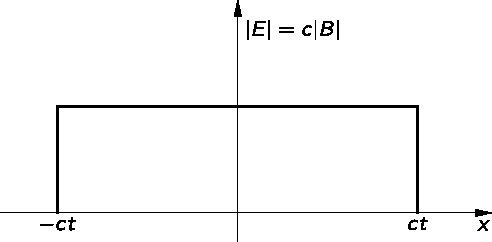
\includegraphics[width=0.7\linewidth]{fyz_fig643.pdf}
      \caption{
               (\cite[s.~707]{Feynman02})}
      \label{fyz:fig643}
    \end{figure}


    \begin{figure}[ht!] %\ref{fyz:fig644}
      \centering
      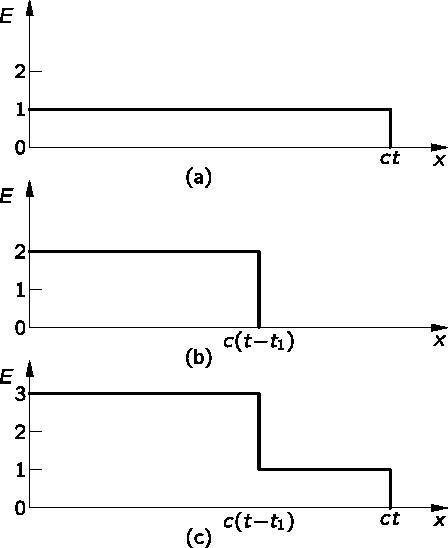
\includegraphics[width=0.7\linewidth]{fyz_fig644.pdf}
      \caption{
               (\cite[s.~707]{Feynman02})}
      \label{fyz:fig644}
    \end{figure}


    \begin{figure}[ht!] %\ref{fyz:fig645}
      \centering
      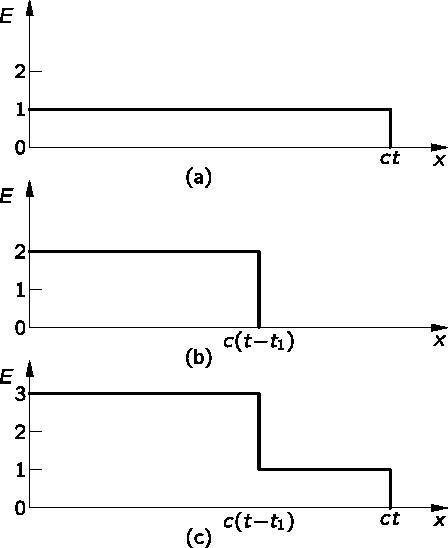
\includegraphics[width=0.7\linewidth]{fyz_fig645.pdf}
      \caption{
               (\cite[s.~707]{Feynman02})}
      \label{fyz:fig645}
    \end{figure}

    \begin{figure}[ht!] %\ref{fyz:fig646}
      \centering
      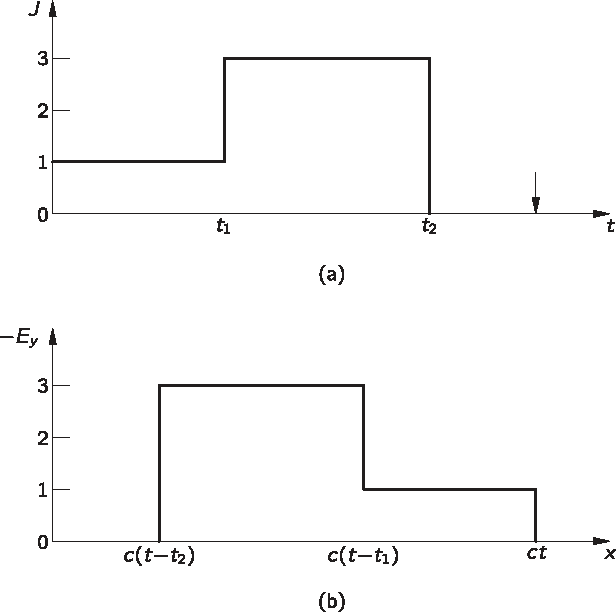
\includegraphics[width=0.7\linewidth]{fyz_fig646.pdf}
      \caption{
               (\cite[s.~707]{Feynman02})}
      \label{fyz:fig646}
    \end{figure}


    \begin{figure}[ht!] %\ref{fyz:fig647}
      \centering
      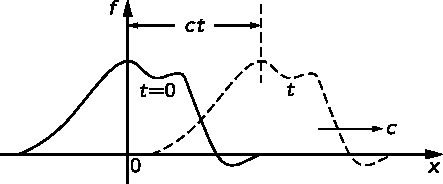
\includegraphics[width=0.7\linewidth]{fyz_fig647.pdf}
      \caption{
               (\cite[s.~707]{Feynman02})}
      \label{fyz:fig647}
    \end{figure}

    \begin{figure}[ht!]
      \centering
      \subcaptionbox{\label{fyz:fig649a}}{\luafigure[0.8]{fyz_fig649a.pdf}}               \\
      \subcaptionbox{\label{fyz:fig649b}}{\luafigure[0.8]{fyz_fig649b.pdf}}
      \label{fyz:fig649}
      \caption{
               (\cite[s.~748]{Feynman02})}
    \end{figure}
    
    \todo[inline]{Kapitola fey2ch20 je nedodělaná, obsahuje pouze obrázky}
%} %tikzset
%---------------------------------------------------------------------------------------------------
  % % !TeX spellcheck = cs_CZ
%{\tikzset{external/prefix={tikz/FYZII/}}
% \tikzset{external/figure name/.add={ch31_}{}}
%---------------------------------------------------------------------------------------------------
% file fey2ch31.tex
%---------------------------------------------------------------------------------------------------
%=========================== Kapitola Tenzory ======================================================
\setchaptertoc
\chapter{Tenzory}\label{fyz:IIchapXXXI}

  \section{Tenzory polarizovatelnosti}\label{fyz:IIchapXXXIsecI}
    Fyzici mají ve zvyku zvolit nejednodušší příklad nějakého jevu a nazvat jej „fyzikou", přičemž
    komplikovanější příklady nechávají na starosti jiným odvětvím, například aplikované matematice,
    elektroinženýrství, chemii nebo krystalografii. Dokonce i fyzika pevných látek je téměř
    „polofyzikou”, neboť se příliš zajímá o speciální látky. Proto i v těchto přednáškách budeme
    vynechávat spoustu zajímavých věcí. Například jednou z důležitých vlastností krystalů, nebo
    většiny látek, je to, že jejich elektrická polarizovatelnost je v různých směrech různá.
    Nachází-li se látka ve elektrickém poli, které má určitý směr, posunou se mírně náboje atomů a
    vytvoří se dipólový moment. Velikost tohoto momentu silně závisí na směru pole. A to je,
    samozřejmě, určitá komplikace. Ale ve fyzice si to zjednodušujeme a obvykle začínáme se
    speciálním případem, kdy je polarizovatelnost stejná ve všech směrech. Ostatní případy necháváme
    na starosti jiným vědním oborům. Proto v našich dalších úvahách vůbec nebudeme potřebovat to, o
    čem budeme mluvit v této kapitole.
    
    Matematika tenzorů je zvláště užitečná při popisu těch vlastností látek, které závisejí na
    směru, ačkoliv je to jen jeden z příkladů jejího využití. Jelikož většina z vás se nemíní stát
    fyziky, ale budete se zabývat reálným světem, kde věci silně závisejí na směru, budete muset
    dříve či později používat tenzory. Abychom nic nevynechávali, pohovoříme o tenzorech. Chceme,
    aby naše chápání fyziky bylo co nejúplnější. Například náš výklad elektrodynamiky je úplný - tak
    úplný jako libovolný kurz elektřiny a magnetizmu, dokonce i pro fyzikální specializace na vysoké
    škole. Mechanika nebyla úplně ukončena, protože, když jsme ji probírali, nebyly ještě naše
    matematické znalosti na takové úrovni, abychom mohli hovořit o tématech, jako je princip
    nejmenšího účinku, lagranžiány, hamiltoniány atd., které představují elegantnější způsob popisu
    mechaniky. Ale s výjimkou obecné teorie relativity jsme všechny zákony mechaniky probrali. Naše
    elektřina a magnetizmus jsou kompletní a mnoho dalších oblastí je v podstatě uzavřeno. Kvantová
    mechanika přirozeně ne; musíme si něco nechat do budoucna. Ale co je tenzor, musíme vědět už
    nyní. 

    V kapitole \ref{fyz:IIchapXXX} jsme zdůrazňovali, že vlastnosti krystalických látek jsou v
    různých směrech různé, říkáme, že jsou anizotropní. Závislost indukovaného dipólového momentu na
    směru vnějšího elektrického pole je jen jedním z možných příkladů, ale právě ten si vybereme
    jako příklad tenzoru. Předpokládejme, že při daném směru elektrického pole je indukovaný
    dipólový moment objemové jednotky \(\vec{P}\) úměrný intenzitě vnějšího pole \(\vec{E}\). (To je
    dobrá aproximace pro většinu látek, pokud \(\vec{E}\) není příliš velké.) Konstantu úměrnosti
    označíme \(\alpha\)\footnote{V kapitole \ref{fyz:IIchapX} jsme souhlasně s konvencí psali
    \(P=\varepsilon_0\chi E\) a \(\chi\) („chí") jsme nazývali \emph{susceptibilita}. Nyni bude
    pohodlnější používat jedno písmeno, proto namísto \(\varepsilon_0\chi\) budeme psát \(\alpha\).
    Pro izotropní dielektrika platí \(\alpha = (\varepsilon_r - 1)\varepsilon_0\), kde
    \(\varepsilon_r\) je relativní permitivita (článek \ref{fyz:IIchapXsecIV})}. Budeme uvažovat
    látky, v nichž \(\alpha\) závisí na směru pole, jako například v krystalech podobných vápenci,
    který má tu vlastnost, že při průhledu vidíme obraz dvojitě. 

    Předpokládejme, že jsme zjistili, že v určitém krystalu vyvolává elektrické pole \(\vec{E}_1\),
    působící ve směru osy \(x\), polarizaci \(\vec{P}_1\) ve směru \(x\). Dále nechť elektrické pole
    \(\vec{E}_2\) ve směru osy \(y\), které má stejnou intenzitu jako \(\vec{E}_1\), vyvolává jinou
    polarizaci \(\vec{P}_2\) ve směru \(y\). Co by se stalo, kdyby elektrické pole působilo pod
    úhlem \ang{45}? Takové pole je superpozicí dvou polí působících podél os \(x\) a \(y\), proto
    polarizace \(\vec{P}\) bude vektorovým součtem \(\vec{P}_1\) a \(\vec{P}_2\), jak je znázorněno
    na obr. \ref{fyz:fig0874a}. Polarizace už nemá tentýž směr jako elektrické pole. Lze pochopit,
    proč tomu tak je. V látce se mohou nacházet náboje, které se mohou snadno posouvat směrem nahoru
    a dolů, ale obtížně se pohybují ze strany na stranu. Když síla působí pod úhlem \ang{45}, náboje
    se posunou víc směrem nahoru než na stranu. Výsledné přemístění nemá směr vnější síly, protože
    tu působí vnitřní elastické síly, které jsou asymetrické.
    
    Úhel \ang{45} není, samozřejmě, nijak výjimečný. Indukovaná polarizace obecně nemá směr
    elektrického pole. V našem předcházejícím příkladě se nám „poštěstilo“ zvolit osy \(x\) a \(y\)
    tak, aby \(\vec{P}\) mělo směr \(\vec{E}\) podél obou os. Kdyby byl krystal pootočen vzhledem k
    osám souřadnic, vyvolalo by elektrické pole \(\vec{E}\) ve směru osy \(y\) polarizaci
    \(\vec{P}\), která by měla obě složky, \(x\) i \(y\). Podobně polarizace, která by vznikla díky
    poli ve směru osy \(x\), by také měla složky \(x\) i \(y\). Polarizace by potom vypadaly tak,
    jak je to na obr. \ref{fyz:fig0874b}, a ne jako na obr. \ref{fyz:fig0874a}. Věci se komplikují,
    ale stále je pro libovolné pole \(\vec{E}\) velikost \(\vec{P}\) \emph{úměrná} velikosti
    \(\vec{E}\). 
    
    Nyní uvažujme obecný případ libovolné orientace krystalu vzhledem k souřadnicovým osám.
    Elektrické pole ve směru osy \(x\) vede k polarizaci \(\vec{P}\) se složkami \(x\), \(y\), a
    \(z\). Můžeme psát
    \begin{equation}\label{fyz:eq236}
      P_x = \alpha_{xx}E_x, \quad P_y = \alpha_{yx}E_x, \quad  P_z = \alpha_{zx}E_x.
    \end{equation}

    Celé naše tvrzení je založeno na tom, že má-li elektrické pole směr osy \(x\), nemusí mít
    polarizace tentýž směr, ale má složky ve směru os \(x\), \(y\), \(z\) a každá z nich je úměrná
    \(E_x\). Konstanty úměrnosti označujeme \(\alpha_{xx}\), \(\alpha_{yx}\), \(\alpha_{zx}\).
    (První index je vztažen k příslušné složce \(\vec{P}\), druhý ke směru elektrického pole.) 
    
    Podobně pro pole ve směru osy \(y\) můžeme psát
    \begin{equation}\label{fyz:eq237}
      P_x = \alpha_{xy}E_y, \quad P_y = \alpha_{yy}E_y, \quad  P_z = \alpha_{zy}E_y.
    \end{equation}

    a pro pole ve směru osy \(z\)
    \begin{equation}\label{fyz:eq238}
      P_x = \alpha_{xz}E_z, \quad P_y = \alpha_{yz}E_z, \quad  P_z = \alpha_{zz}E_z.
    \end{equation}

    \begin{figure}[ht!]   %\ref{fyz:fig0874}
      \centering
      \subcaptionbox{\label{fyz:fig0874a}}{\luafigure[0.45]{fyz_fig0874a.pdf}}
      \subcaptionbox{\label{fyz:fig0874b}}{\luafigure[0.45]{fyz_fig0874b.pdf}}
      \caption{Vektorový součet polarizací v anizotropním krystalu (\cite[s.~748]{Feynman02})}
      \label{fyz:fig0874}
    \end{figure}

    Řekli jsme, že polarizace závisí na polích lineárně, proto má-li elektrické pole \(\vec{E}\)
    složku \(x\) i \(y\), bude výsledná \(x\)-ová složka \(\vec{P}\) součtem dvou \(P_x\) z rovnic
    (\ref{fyz:eq236}) a (\ref{fyz:eq237}). Má-li \(\vec{E}\) složky \(x\), \(y\) a \(z\) budou
    výsledné složky \(\vec{P}\) součtem tří příspěvků z rovnic (\ref{fyz:eq236}),
    (\ref{fyz:eq237}), (\ref{fyz:eq238}). Jinými slovy \(\vec{P}\) bude určeno rovnicemi
    \begin{align}\label{fyz:eq240}
      P_x &= \alpha_{xx}E_x + \alpha_{xy}E_y + \alpha_{xz}E_z  \nonumber \\
      P_y &= \alpha_{yx}E_x + \alpha_{yy}E_y + \alpha_{yz}E_z            \\
      P_z &= \alpha_{zx}E_x + \alpha_{zy}E_y + \alpha_{zz}E_z. \nonumber
    \end{align}

    Dielektrické vlastnosti krystalu jsou pak zcela určeny devíti veličinami (\(\alpha_{xx}\),
    \(\alpha_{xy}\), \(\alpha_{xz}\), \(\alpha_{yz}\) \(\ldots\)), které mohou být reprezentovány
    symbolem \(\alpha_{ij}\). (Indexy \(i\), \(j\) zastupují libovolné ze tří písmen \(x\), \(y\),
    \(z\)). Libovolné elektrické pole \(\vec{E}\) může být rozloženo na složky \(E_x\), \(E_y\),
    \(E_z\). Z nich můžeme použitím \(\alpha_{ij}\) najít \(P_x\), \(P_y\) a \(P_z\), které nám
    spolu určují polarizaci \(\vec{P}\). Soubor devíti koeficientů \(\alpha_{ij}\) se nazývá
    \textbf{tenzor} - v tomto případě \textbf{tenzor polarizovatelnosti}. Když říkáme, že tři čísla
    (\(E_x\), \(E_y\), \(E_z\)) tvoří vektor \(\vec{E}\), stejně říkáme, že devět čísel
    (\(\alpha_{xx}\), \(\alpha_{xy}\), \(\alpha_{xz}\), \(\alpha_{yz}\) \(\ldots\)) tvoří tenzor
    \(\alpha_{ij}\). 

  \twocolumn[\section{Transformace tenzorových složek}\label{fyz:IIchapXXXIsecII}]
    Víme, že při přechodu k nové souřadnicové soustavě \(x'\), \(y'\), \(z'\) dostáváme jiné složky
    \(E_{x'}\), \(E_{y'}\),  \(E_{z'}\) vektoru \(\vec{E}\) a stejně i jiné \emph{složky} vektoru
    \(\vec{P}\). Proto všechny koeficienty \(\alpha_{ij}\) mají různou hodnotu v různých
    souřadnicových soustavách. Změnu koeficientů \(\alpha\) při změně \(\vec{E}\) a \(\vec{P}\) lze
    zjistit, neboť popisujeme-li \emph{stejné fyzikální} elektrické pole v nové souřadnicové
    soustavě, měli bychom dostat stejnou polarizaci. Pro libovolnou novou souřadnicovou soustavu je
    \(P_{x'}\) lineární kombinací \(P_{x}\), \(P_{y}\), a \(P_{z}\):
    \begin{equation*}
      P_{x'} = aP_x + bP_y + cP_z.
    \end{equation*}
    Podobně je to i pro ostatní složky. Dosadíme-li za \(P_{x}\), \(P_{y}\), a \(P_{z}\), jejich
    vyjádření pomocí \(\vec{E}\) rovnic (\ref{fyz:eq240}), dostaneme
    \begin{align*}
      P_{x'} = &a(\alpha_{xx}E_x + \alpha_{xy}E_y + \alpha_{xz}E_z) + \\
               &b(\alpha_{yx}E_x + \alpha_{yy}E_y + \alpha_{yz}E_z) + \\
               &c(\alpha_{zx}E_x + \alpha_{zy}E_y + \alpha_{zz}E_z).
    \end{align*}
    Pak vyjádříme \(E_{x}\), \(E_{y}\), a \(E_{z}\), pomocí \(E_{x'}\), \(E_{y'}\), a \(E_{z'}\),
    například
    \begin{equation*}
      E_x =  a'E_x + b'E_y + c'E_z,
    \end{equation*}
    kde \(a'\), \(b'\), \(c'\) jsou v nějakém vztahu k \(a\), \(b\), \(c\), ale navzájem si nejsou
    rovny. Vyjádřili jsme tedy \(P_{x'}\) pomocí složek \(E_{x'}\), \(E_{y'}\), a \(E_{z'}\), tj.
    máme nové \(\alpha_{ij}\). To je trochu neuspořádaný, ale přímočarý postup.

    Když mluvíme o změně os, předpokládáme, že poloha krystalu v prostoru je fixována. Kdyby se
    krystal otáčel \emph{společně} s osami, koeficienty \(\alpha\) by se neměnily. Naopak, kdyby se
    orientace krystalu vzhledem k osám změnila, dostali bychom nový soubor hodnot \(\alpha\).
    Známe-li však koeficienty \(\alpha\) pro nějakou libovolnou orientaci krystalu, můžeme je najít
    pro libovolnou jinou orientaci pomocí transformace, kterou jsme právě popsali. Jinými slovy,
    dielektrické vlastnosti jsou \emph{úplně} popsány zadáním složek polarizovatelnosti tenzoru
    \(\alpha_{ij}\) vzhledem k libovolně zvolené soustavě souřadnic. Stejně jako částici přiřazujeme
    vektor rychlosti \(\vec{v} = (v_x, v_y, v_z)\), vědomi si toho, že tři složky se určitým
    způsobem mění při změně souřadnicových os, podobně krystalu přiřazujeme tenzor
    polarizovatelnosti \(\alpha_{ij}\), jehož devět složek se při změně souřadnicové soustavy
    transformuje určitým způsobem.

    Vztah mezi \(\vec{P}\) a \(\vec{E}\) určený rovnicí (\ref{fyz:eq240}) můžeme zapsat ve zkráceném
    tvaru
    \begin{equation}\label{fyz:eq241}
      P_i = \sum_j\alpha_{ij}E_j,
    \end{equation}

    kde \(i\) označuje některé z písmen \(x\), \(y\) nebo \(z\) a sčítáme přes \(j = x, y, z\). Pro
    operace s tenzory bylo vynalezeno mnoho speciálních označení, ale každé z nich se hodí jen pro
    omezenou třídu problémů. Jednou z obecných konvencí je vynechávání sumačního znaku \(\sum\) v
    rovnici (\ref{fyz:eq241}), přičemž se rozumí, že všude, kde se stejný index vyskytuje dvakrát (v
    našem případě \(j\)), musíme sčítat přes všechny jeho hodnoty. Jelikož tenzory nebudeme používat
    často, nebudeme se trápit s výběrem speciálních označení a konvencí.

  \section{Elipsoid energie}\label{fyz:IIchapXXXIsecIII}
    Nyní si vyzkoušejme, jak se zachází s tenzory. Položíme si zajímavou otázku: Jaká energie je
    potřebná k polarizaci krystalu (kromě energie elektrického pole, o níž víme, že je rovna
    \(\varepsilon_0E^2/2\) pro objemovou jednotku)? Zamyslíme se nad atomovými náboji, které se
    posouvají. Práce, která je vykonána při přemisťování náboje o vzdálenost \(\dd{x}\), je
    \(qE_x\dd{x}\) a je-li v jednotkovém objemu \(N\) nábojů, je vykonaná práce  \(qE_xN\dd{x}\).
    Ale  \(qN\dd{x}\) je změna \(qP_x\), dipólového momentu objemové jednotky. Proto energie
    připadající na \emph{objemovou jednotku} je
    \begin{equation*}
      E_x\dd{P_x}.
    \end{equation*}

    Sečteme-li práci všech tří složek pole, pro práci připadající na objemovou jednotku dostaneme
    \begin{equation*}
      \vec{E}\cdot\dd{P}.
    \end{equation*}
    Jelikož velikost \(\vec{P}\) je úměrná \(\vec{E}\), bude práce vykonaná při polarizování
    objemové jednotky od 0 do \(\vec{P}\) rovna integrálu výrazu \(\vec{E}\cdot\dd{P}\). Označíme-li
    tuto práci \(\omega_p\), můžeme psát\footnote{Je to práce spotřebovaná na vytvoření polarizace
    elektrickým polem a není možné ji zaměňovat s potenciální energií \(-\vec{p}_o\cdot\vec{E}\).
    konstantního dipólového momentu \(\vec{p}_o\).}
    \begin{equation}\label{fyz:eq242}
      \omega_p = \frac{1}{2}\vec{E}\cdot\vec{P} = \frac{1}{2}\sum_iE_iP_i.
    \end{equation}

    Nyní můžeme vyjádřit \(\vec{P}\) pomocí \(\vec{E}\) použitím rovnice (\ref{fyz:eq241}) a
    dostaneme
    \begin{equation}\label{fyz:eq243}
      \omega_p = \frac{1}{2}\sum_i\sum_j\alpha_{ij}E_iE_j.
    \end{equation}
    Hustota energie \(w_p\), je číslo, které nezávisí na výběru os, je to tedy skalár. Tenzor
    \(\alpha_{ij}\) bychom měli správně nazývat tenzor druhého řádu, neboť má dva indexy. Vektor (s
    \emph{jedním} indexem je tenzor prvního řádu a skalár (bez indexu) je tenzor nultého řádu.
    Říkáme, že elektrické pole \(\vec{E}\) je tenzor prvního řádu a že hustota energie \(w_p\) je
    tenzor nultého řádu. Pojem tenzoru bychom mohli rozšířit na tři a víc indexů, a tak bychom
    sestrojili tenzory vyššího než druhého řádu.

    Indexy tenzoru polarizovatelnosti mohou nabývat tří různých hodnot - je to trojrozměrný tenzor.
    Matematici uvažují tenzory ve čtyřech, pěti nebo vyšších rozměrech. My jsme už používali
    čtyřrozměrný tenzor \(\vec{F}_{\mu\nu}\), při našem relativistickém popisu elektromagnetického
    pole (kapitola \ref{fyz:IIchapXXVI}).

    \luagraphic[0.8]{fyz_fig0875.pdf}{Množina koncových bodů vektoru \(\vec{E} = (E_x, E_y)\), který
    odpovídá konstantní energii polarizace (\cite[s.~577]{Feynman02})}{fyz:fig0875}

    Tenzor polarizovatelnosti \(\alpha_{ij}\) má tu zajímavou vlastnost, že je symetrický, to
    znamená, že \(\alpha_{xy} = \alpha_{yx}\), a totéž platí pro libovolnou dvojici indexů. (To je
    \emph{fyzikální} vlastnost reálného krystalu, a neplatí nevyhnutelně pro všechny tenzory.)
    Můžete si sami dokázat, že to tak musí být, výpočtem změny energie krystalu následujícím
    postupem: 1. Zapněte elektrické pole ve směru osy \(x\). 2. Zapněte pole ve směru osy \(y\). 3.
    Vypněte pole ve směru osy \(x\). 4. Vypněte pole ve směru osy \(y\).

    Krystal je nyní v takovém stavu, jako byl na začátku, a celková práce spotřebovaná na polarizaci
    musí být rovna nule. Lze však ukázat, že má-li to být pravda, musí být \(\alpha_{xy}\), rovno
    \(\alpha_{yx}\). Stejné úvahy můžeme, samozřejmě, aplikovat i na \(\alpha_{xz}\), atd.
    \emph{Tenzor polarizovatelnosti je tedy symetrický}.

    To také znamená, že tenzor polarizovatelnosti můžeme určit změřením energie potřebné k
    polarizaci krystalu v různých směrech. Předpokládejme, že pole \(\vec{E}\) působí jen ve směru
    os \(x\) a \(y\). Pak souhlasně s rovnicí (\ref{fyz:eq243}) pro \(\omega_p\) dostáváme
    \begin{equation}\label{fyz:eq244}
      \frac{1}{2}\left(\alpha_{xx}E_x^2 + (\alpha_{xy} + \alpha_{yx})E_xE_y + \alpha_{yy}E_y^2\right).
    \end{equation}

    Kdybychom měli jen složku \(E_x\), mohli bychom určit \(\alpha_{xx}\) v případě složky \(E_y\)
    můžeme určit \(\alpha_{yy}\), máme-li zároveň \(E_x\) i \(E_y\), dostáváme energii pocházející
    ze členu s \(\alpha_{xy} + \alpha_{yx}\). Jelikož \(\alpha_{xy}\) a \(\alpha_{yx}\) jsou si
    navzájem rovny, je tento člen úměrný \(2\alpha_{xy}\) a lze jej určit z energie.

    výraz pro energii \eqref{fyz:eq244} má pěknou geometrickou interpretaci. Předpokládejme, že se
    ptáme, jaká pole \(E_x\) a \(E_y\) odpovídají dané hustotě energie, například \(\omega_0\). Je
    to matematická úloha řešení rovnice:
    \begin{equation*}
      \alpha_{xx}E_x^2 + 2\alpha_{xy}E_xE_y + \alpha_{yy}E_y^2 = 2\omega_0.
    \end{equation*}

    To je \emph{kvadratická rovnice}, proto při grafickém znázornění této rovnice (obr.
    \ref{fyz:fig0875}) budou všechna řešení \(E_x\) a \(E_y\) ležet na elipse. (Musí to být elipsa, a
    ne parabola nebo hyperbola, neboť energie je pro libovolné pole vždy kladná a konečná.) Vektor
    \(\vec{E}\) se složkami \(E_x\) a \(E_y\) bude znázorněn tak, že jeho počátek je v počátku
    souřadnic a koncový bod leží na elipse. Pomocí této „energetické elipsy“ názorně vidíme jak
    „vypadá“ polarizační tenzor.

    \luagraphic[0.7]{fyz_fig0876.pdf}{Elipsoid energie tenzoru polarizovatelnosti
    (\cite[s.~577]{Feynman02})}{fyz:fig0876}
    
    Vezmeme-li nyní v úvahu všechny tři složky vektoru \(\vec{E}\) libovolného směru, který vede k
    jednotkové hustotě energie, budou jeho koncové body ležet na povrchu \textbf{elipsoidu}, jak je
    to na obr. \ref{fyz:fig0876}. Tvar tohoto elipsoidu konstantní energie jednoznačně určuje tenzor
    polarizovatelnosti.

    Elipsoid má pěknou vlastnost, že vždy může být popsán prostě zadáním směrů tří hlavních os a
    průměry elipsoidu podél těchto os. Hlavní osy - osy ve směru nejdelšího a nejkratšího průměru a
    ve směru kolmém na obě tyto osy. Na obr. \ref{fyz:fig0876} jsou označeny jako \(a\), \(b\),
    \(c\). Vzhledem k těmto osám nabývá rovnice elipsoidu obzvlášť jednoduchého tvaru
    \begin{equation*}
      \alpha_{aa}E_a^2 + \alpha_{bb}E_b^2 + \alpha_{cc}E_c^2= 2\omega_0.
    \end{equation*}

    Tenzor polarizovatelnosti má tedy jen tři nenulové složky: \(\alpha_{aa}\), \(\alpha_{bb}\) a
    \(\alpha_{cc}\). To znamená, že pro libovolně komplikovaný krystal je vždy možné vybrat jen
    takové osy (nemusí to být osy krystalu), pro které má náš tenzor jen tři složky. Pro takové osy
    nabývají rovnice \eqref{fyz:eq240} jednoduchý tvar
    \begin{equation}\label{fyz:eq832}
      P_a = \alpha_{aa}E_a,\quad P_b = \alpha_{bb}E_b,\quad P_a = \alpha_{cc}E_c.
    \end{equation}
    Elektrické pole podél jedné z hlavních os vyvolává polarizaci podél téže osy, ale, samozřejmě,
    koeficienty, které patří třem osám, mohou být různé.

    Tenzor často píšeme jako tabulku devíti koeficientů uvnitř závorek
    \begin{equation}\label{fyz:eq938} 
      \begin{bmatrix}
        \alpha_{xx}& \alpha_{xy}& \alpha_{xz} \\
        \alpha_{yx}& \alpha_{yy}& \alpha_{yz} \\
        \alpha_{zx}& \alpha_{zy}& \alpha_{zz}
      \end{bmatrix}.
    \end{equation}

    Pro hlavní osy \(a\), \(b\), \(c\) jsou jen diagonální členy různé od nuly. Říkáme, že tenzor je
    diagonální a jeho tvar je
    \begin{equation}\label{fyz:eq939}
      \begin{bmatrix}
        \alpha_{aa}&      0      &      0      \\
             0     & \alpha_{bb} &      0      \\
             0     &      0      & \alpha_{cc}
      \end{bmatrix}.
    \end{equation}
    Důležitým faktorem je, že libovolný tenzor polarizovatelnosti (ve skutečnosti libovolný
    symetrický tenzor druhého stupně pro libovolný počet rozměrů) se může v tomto tvaru psát při
    vhodném výběru souřadnicových os.
    
    Jsou-li si tři prvky polarizačního vektoru v diagonálním tvaru rovny,
    \begin{equation}\label{fyz:eq940}
        \alpha_{aa} = \alpha_{bb} = \alpha_{cc} = \alpha,
    \end{equation}
    stává se \emph{elipsoid energie kulovou plochou} a polarizovatelnost je stejná ve všech směrech.
    Látka je \emph{izotropní}. V tenzorovém označení
    \begin{equation}\label{fyz:eq946}
      \alpha_{ij} = \alpha\delta_{ij},
    \end{equation}
    kde \(\delta_{ij}\) je \textbf{jednotkový tenzor}
    \begin{equation}\label{fyz:eq942}
      \delta_{ij} = 
      \begin{bmatrix}
             1 & 0 & 0 \\
             0 & 1 & 0 \\
             0 & 0 & 1  
      \end{bmatrix}.
    \end{equation}
    To samozřejmě znamená, že
    \begin{equation}\label{fyz:eq943}
      \delta_{ij} = 
      \begin{cases} 
         1  & \text{pro } i = j     \\
         0  & \text{pro } i \neq j.
      \end{cases}
    \end{equation}

    Tenzor \(\delta_{ij}\) se často nazývá \textbf{Kroneckerovo delta}. Můžeme se pobavit tím, že
    dokážeme, že tenzor \eqref{fyz:eq942} bude mít po záměně jedné pravoúhlé soustavy za druhou
    přesně tutéž formu. Tenzor polarizovatelnosti typu \eqref{fyz:eq946} nám dává
    \begin{equation*}
      P_i = \alpha\sum_j\delta_{ij}E_j = \alpha E_i,
    \end{equation*}
    což je totéž jako náš starý výsledek pro izotropní dielektrika
    \begin{equation*}
      \vec{P} = \alpha\vec{E},
    \end{equation*}

    Tvar a orientace elipsoidu polarizovatelnosti může někdy souviset s vlastnosti symetrie
    krystalu. V kapitole \ref{fyz:IIchapXXX} jsme řekli, že existuje 230 různých možných symetrií
    trojrozměrné mřížky a pro různé účely je vhodné je rozdělit na sedm tříd podle tvaru základní
    buňky. Elipsoid polarizovatelnosti musí odrážet vnitřní symetrii krystalu. Například trojklonný
    krystal má nízkou symetrii - elipsoid polarizovatelnosti bude mít nestejné osy a jejich
    orientace nebude obecně souhlasit se směrem os krystalu. Na druhé straně má jednoklonná mřížka
    tu vlastnost, že při rotaci o \ang{180} kolem jedné osy se její vlastnosti nemění. Proto
    polarizační tenzor musí při takové rotaci zůstávat nezměněn. Z toho vyplývá, že tenzor
    polarizovatelnosti se po rotaci o \ang{180} musí transformovat sám v sebe. To je možné jen v tom
    případě, kdy jedna z os elipsoidu má tentýž směr jako osa symetrie krystalu. Žádná další omezení
    na orientaci a rozměry elipsoidu nejsou.
    
    Pro kosočtverečný krystal však musí osy elipsoidu souhlasit s osami krystalu, neboť při rotaci o
    \ang{180} kolem libovolné ze tří os dostáváme tutéž mřížku. Vezmeme-li čtverečný krystal, musí
    mít elipsoid stejnou symetrii, tj. musí mít dva průměry stejné. Nakonec, pro krychlový krystal
    musí být všechny tři průměry elipsoidu stejné. Elipsoid se stává kulovou plochou a
    polarizovatelnost krystalu je ve všech směrech stejná.
    
    Existuje celá věda o určování druhů tenzorů pro všechny možné symetrie krystalu. Je to analýza
    založená na teorii grup. Ale pro jednoduché případy tenzoru polarizovatelnosti je poměrně snadno
    vidět, jaké musí příslušné vztahy být.

  \section{Tenzor setrvačnosti}\label{fyz:IIchapXXXIsecIV} 
  
    Ve fyzice najdeme mnohé další příklady tenzorů. Například v kovu nebo v libovolném vodiči bývá
    často proudová hustota \(\vec{j}\) přibližně úměrná elektrickému poli \(\vec{E}\). Konstanta
    úměrnosti a se nazývá měrná \emph{vodivost} (konduktivita):
    \begin{equation*}
      \vec{j} = \sigma\vec{E}.
    \end{equation*}
    Pro krystaly je však vztah mezi \(\vec{j}\) a \(\vec{E}\) mnohem komplikovanější, vodivost není
    stejná ve všech směrech. Konduktivita je tenzorem, proto píšeme
    \begin{equation*}
      j_i = \sum_j\sigma_{ij}E_j
    \end{equation*}

    Dalším příkladem fyzikálního tenzoru je moment setrvačnosti. V \ref{fyz:IchapXVIII}. kapitole
    \ref{part:FYZI}. dílu jsme viděli, že při rotaci tuhého tělesa kolem fixované osy jejeho moment
    hybnosti \(L\) úměrný úhlové rychlosti \(ω\) a koeficient úměrnosti \(L\) jsme nazvali
    \emph{momentem setrvačnosti} \[L=I\omega\].

    Moment setrvačnosti libovolně tvarovaného tělesa závisí na jeho orientaci vzhledem k ose
    otáčení. Například kvádr bude mít různé momenty vzhledem ke každé z jeho tří navzájem kolmých
    os. Úhlové rychlosti \(\vec{ω}\) i moment hybnosti \(\vec{L}\) jsou vektory. Při rotaci kolem
    jedné z os symetrie jsou tyto vektory rovnoběžné. Avšak jsou-li momenty setrvačnosti vzhledem ke
    třem hlavním osám různé, nemusí být \(\vec{ω}\) a \(\vec{L}\) vždy rovnoběžné (obr.
    \ref{fyz:fig0877}). Jejich vzájemný vztah je podobný jako vztah mezi \(\vec{E}\) a \(\vec{P}\).
    Obecně musíme psát
    \begin{align}
      Lx&=I_{xx}=I_{xx}ω_x+I_{xy}ω_y+I_{xz}ω_z,  \nonumber         \\
      Ly&=I_{yx}=I_{yx}ω_x+I_{yy}ω_y+I_{yz}ω_z,  \label{fyz:eq944} \\
      Lz&=I_{zx}=I_{zx}ω_x+I_{zy}ω_y+I_{zz}ω_z.  \nonumber 
    \end{align}
    Devět koeficientů \(I_{ij}\). je nazýváno \textbf{tenzor setrvačnosti}. Podobně jako v případě
    polarizace musí být kinetická energie pro libovolný moment hybnosti kvadratickou formou vzhledem
    k \(ω_x\), \(ω_y\) a \(ω_z\):
    \begin{equation}\label{fyz:eq945}
      E_k = \frac{1}{2}\sum_{ij}L_{ij}ω_iω_j.
    \end{equation}
    Energii můžeme využít k definování \textbf{elipsoidu setrvačnosti}. Opět můžeme pomocí úvah o
    energii dokázat, že tenzor setrvačnosti je \emph{symetrický}, tj. že \(I_{ij} = I_{ji}\)

    Tenzor setrvačnosti tuhého tělesa můžeme určit, zname-li jeho tvar. Potřebujeme jen napsat
    kinetickou energii všech částic tělesa. Částice, která má hmotnost \(m\) a rychlost \(\vec{v}\),
    má kinetickou energii \(\sfrac{1}{2}mv^2\) a celková kinetická energie je součtem výrazů
    \[\sum\frac{1}{2}mv^2\] pocházejících od všech částic tělesa. Rychlost \(\vec{v}\) každé částice
    souvisí s úhlovou rychlostí \(\vec{ω}\) tuhého tělesa. Předpokládejme, že těleso se otáčí kolem
    svého těžiště, které je v klidu. Je-li \(\vec{r}\) polohový vektor částice vzhledem k těžišti,
    rychlost částice \(\vec{v}\) je dána výrazem \(\vec{ω}\times\vec{r}\). Celková kinetická energie
    je
    \begin{equation}\label{fyz:eq948}
      E_k = \sum\frac{1}{2}m\left(\vec{ω}\times\vec{r}\right)^2.
    \end{equation}

    \luagraphic[0.7]{fyz_fig0877.pdf}{Moment hybnosti \(\vec{L}\) tuhého tělesa obecně není
    rovnoběžný s úhlovou rychlostí \(\vec{ω}\) (\cite[s.~580]{Feynman02})}{fyz:fig0877}
    
    Nyní už jen stačí rozepsat \(\vec{ω}\times\vec{r}\) pomocí složek \(ω_x\), \(ω_y\) a \(ω_z\) a
    \(x\), \(y\), \(z\) a porovnat výsledek s rovnicí \eqref{fyz:eq945}. \(I_{ij}\) najdeme
    porovnáním jednotlivých členů. Provedeme algebraické úpravy
    \begin{equation*}
      (\vec{ω}×\vec{r})^2=(\vec{ω}×\vec{r})^2_x+(\vec{ω}×\vec{r})^2_y+(\vec{ω}×\vec{r})^2_z
    \end{equation*}
    čili
    \begin{equation*}
      (ω_yz−ω_zy)^2+(ω_zx−ω_xz)^2+(ω_xy−ω_yx)^2
    \end{equation*}
    a konečně
    \begin{align*}
      = &+ω_y^2z − 2ω_yω_z zy + ω_z^2y^2 \\
        &+ω_z^2x − 2ω_zω_x xz + ω_x^2z^2 \\
        &+ω_x^2y − 2ω_xω_y yx + ω_y^2x^2.
    \end{align*}
    Vynásobřme-li tuto rovnici veličinou \(\sfrac{m}{2}\) sečteme přes všechny částice a porovnáme s
    rovnicí \eqref{fyz:eq945}, zjistíme, že například \(I_{xx}\) je rovno
    \begin{equation*}
      I_{xx}=∑m(y^2+z^2).
    \end{equation*}
    Je to tentýž vzorec, který jsme dostali v \ref{fyz:IchapXIX}. kapitole \ref{part:FYZI}. dílu pro
    moment setrvačnosti tělesa vzhledem k ose \(x\). Jelikož \(r^2 = x^2 + y^2 + z^2\) můžeme tento
    vzorec psát i jako
    \begin{equation*}
      I_{xx}=∑m(r^2-x^2).
    \end{equation*}
    Vypíšeme-li všechny ostatní členy tenzoru setrvačnosti \(I_{ij}\), dostaneme
    \begin{equation*}
      \begin{bmatrix}
        \sum m(r^2-x^2) &    -\sum mxy     &   -\sum mxz     \\
          -\sum myx     &  \sum m(r^2-y^2) &   -\sum myz     \\
          -\sum mzx     &    -\sum mzy     & \sum m(r^2-z^2)
      \end{bmatrix}.
    \end{equation*}
    Chceme-li, můžete si to zapsat v tenzorovém označení jako
    \begin{equation}\label{fyz:eq949}
      I_{ij}=\sum m(r^2\delta_{ij}-r_ir_j),
    \end{equation}
    kde \(r_i\) jsou složky \((x, y, z)\) polohového vektoru částice a \(\sum\) označuje sumu přes
    všechny částice. \emph{Moment setrvačnosti je tedy tenzorem druhého řádu}. Jeho členy jsou
    určeny vlastnostmi tělesa a vztah mezi \(\vv{L}\) a \(\vv{\omega}\) je vyjádřen pomocí tohoto
    tenzoru jako
    \begin{equation}\label{fyz:eq950}
      L_i=\sum_jI_{ij}\omega_j.
    \end{equation}
    Pro těleso libovolného tvaru lze najít elipsoid setrvačnosti, a tedy i tři hlavní osy. Vzhledem
    k těmto osám bude tenzor diagonální, tj. pro libovolný objekt existují vždy tři navzájem kolmé
    osy, pro něž jsou úhlová rychlost a moment hybnosti paralelní. Nazývají se \textbf{hlavní osy
    setrvačnosti}.

  \section{Vektorový součin}\label{fyz:IIchapXXXIsecV}   
    Vzpomeňme si, že tenzory druhého řádu jsme používali už od \ref{fyz:IchapXX}. kapitoly
    \ref{part:FYZI}. dílu. Tehdy jsme definovali \emph{moment síly v rovině}, například složku
    \(N_{xy}\) vztahem 
    \begin{equation*}
      N_{xy} = xF_y-yF_x.
    \end{equation*}
    Po zobecnění na tři rozměry lze psát
    \begin{equation}\label{fyz:eq947}
      N_{ij} = r_iF_j-r_jF_i.
    \end{equation}
    Veličina \(N_{ij}\) je \emph{tenzor druhého řádu}. Lze to ukázat například tak, že zkombinujeme
    \(N_{ij}\) s nějakým vektorem, řekněme s jednotkovým vektorem \(\vec{e}\), tímto způsobem:
    \begin{equation*}
      \sum_jN_{ij}e_j.
    \end{equation*}
    Je-li takováto veličina \emph{vektor}; musí se \(N_{ij}\) transformovat jako tenzor - to je naše
    definice tenzoru. Dosadíme za \(N_{ij}\) a dostaneme
    \begin{align*}
      \sum_jN_{ij}e_j
        &=\sum_jr_iF_je_j-\sum_jr_je_jF_i           \\[1ex]
        &=r_i(\vec{F}\cdot\vec{e})-(\vec{r}\cdot\vec{e})F_i.
    \end{align*}
    Jelikož skalární součin je skalár, jsou dva členy na pravé straně rovnice vektory a vektorem je
    i jejich rozdíl. \(N_{ij}\) je tedy tenzor.

    Ale \(N_{ij}\) je speciálním druhem tenzoru - je to \textbf{antisymetrický tenzor}, pro nějž
    platí
    \begin{equation*}
      N_{ij}=-N_{ji},
    \end{equation*}
    tj. má jen tři nenulové členy \(-N_{xy}\), \(N_{yz}\) a \(N_{zx}\). V \ref{fyz:IchapXX}.
    kapitole \ref{part:FYZI}. dílu se nám podařilo ukázat, že tyto tři členy se téměř \uv{náhodou}
    transformují jako tři složky vektoru, takže jsme mohli \emph{definovat}
    \begin{equation*}
      N = N_{ij}=-N_{ji},
    \end{equation*}
    
    Říkáme „náhodou“, neboť toto platí jen v trojrozměrném případě. Pro čtyři rozměry má například
    antisymetrický tenzor druhého řádu šest nenulových složek a, samozřejmě, nemůže být nahrazen
    vektorem se čtyřmi složkami.
    \begin{equation*}
      \vec{N}=(N_x,N_y,N_z)=(N_{yz},N_{zx},N_{xy})
      \end{equation*}
    Stejně jako axiální vektor \(\vec{N}=\vec{r}\times\vec{F}\) je tenzorem, i každý vektorový
    součin dvou polárních vektorů je tenzorem. Lze použít stejné argumenty. Naštěstí je možné je
    psát jako vektory (přesněji pseudovektory), což nám zjednodušuje naši matematiku.
    
    Matematicky, jsou-li \(\vec{a}\) a \(\vec{b}\) libovolné dva vektory, tvoří devět veličin
    \(a_ib_j\) tenzor (ačkoliv nemusí mít žádný fyzikální význam). Tak dostáváme z polohového
    vektoru \(r_i\). tenzor \(r_ir_j\) a jelikož \(\delta_{ij}\) je také tenzor, je pravá strana
    rovnice \eqref{fyz:eq949} tenzor. Podobně rovnice \eqref{fyz:eq947} je tenzor, jelikož oba členy
    na pravé straně jsou tenzory.

  \section{Tenzor napětí}\label{fyz:IIchapXXXIsecVI} 

    Symetrické tenzory, s nimiž jsme se dosud setkali, vznikly z koeficientů, které dávaly do
    vzájemného vztahu dva vektory. Nyní se seznámíme s tenzorem, který má jiný fyzikální význam - s
    \textbf{tenzorem napětí}. Předpokládejme, že máme pevné těleso, na nějž působí různé síly.
    Říkáme, že uvnitř působí různá „napětí“, čímž rozumíme, že mezi sousedními částicemi látky
    působí vnitřní síly. O takových napětích jsme se zmínili už v článku \ref{fyz:IIchapXIIsecIII},
    když jsme uvažovali dvojrozměrný případ povrchového napětí napnuté membrány. Nyní si ukážeme, že
    vnitřní síly působící v látce trojrozměrného tělesa mohou být popsány pomocí tenzoru.

    \begin{figure}[ht!] %\ref{fyz:fig0878}
      \centering
      \subcaptionbox{\label{fyz:fig0878a}}{\luafigure[0.45]{fyz_fig0878a.pdf}}
      \subcaptionbox{\label{fyz:fig0878b}}{\luafigure[0.45]{fyz_fig0878b.pdf}}
      \caption{Látka nalevo od roviny \(\sigma\) působí přes plošku \(\Delta x\Delta y\) silou
              \(\Delta F_1\), na látku napravo (\cite[s.~583]{Feynman02})}
      \label{fyz:fig0878}
    \end{figure}

    Uvažujme těleso z nějakého pružného materiálu, například kostku želatiny. Když je rozřízneme,
    látka se na obou stranách řezu působením vnitřních sil posune. Předtím, než jsme řez provedli,
    musely mezi oběma částmi kostky existovat síly, které udržovaly látku pohromadě: napětí můžeme
    definovat pomocí těchto sil. Představme si rovinu kolmou na osu \(x\) (jako je rovina \(\sigma\)
    na obr. \ref{fyz:fig0879}) a ptáme se na síly působící na malou plošku \(\Delta y\Delta z\) této
    roviny. Látka nalevo od plošky působí silou \(Δ\vec{F_1}\) na látku napravo tak, jak je
    znázorněno na obrázku \ref{fyz:fig0878b}. Na látku nalevo od plochy působí, samozřejmě, opačná
    síly reakce \(-Δ\vec{F_1}\). Je-li ploška dostatečně malá, očekáváme, že síla \(Δ\vec{F_1}\)? je
    úměrná velikosti plochy \(\Delta y\Delta z\).

    \begin{figure}[ht!] %\ref{fyz:fig0879}
      \centering
      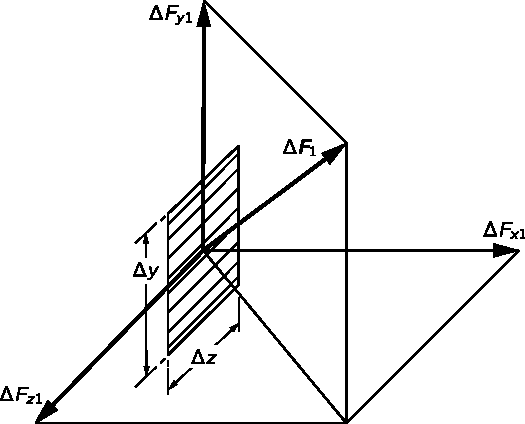
\includegraphics[width=0.8\linewidth]{fyz_fig0879.pdf}
      \caption{\(\Delta F_1\) působící na plošný element \(\Delta y\Delta z\) kolmý na osu \(x\) se
              rozkládá na tři složky \(\Delta F_{x1}\), \(\Delta F_{y1}\) a \(\Delta F_{z1}\)
              (\cite[s.~584]{Feynman02})}
      \label{fyz:fig0879}
    \end{figure}

    Jeden druh napětí už známe, a to statický tlak v kapalině. V tom případě je síla kolmá na
    povrchový element a je rovna tlaku vynásobenému povrchem. Pro pevné látky (jakož i pro
    pohybující se viskózní kapaliny) nemusí být síla kolmá na povrch, působí tu kromě tlaků
    (kladných nebo záporných) i \textbf{smykové síly}. (Smykovou silou rozumíme \emph{tangenciální}
    složku síly působící na povrch.) Všechny tři složky síly je třeba vzít v úvahu. Všimněme si, že
    bude-li mít náš řez rovinou jinou orientaci, budou síly jiné. K úplnému popisu vnitřního napětí
    potřebujeme tenzor.
    
    \emph{Tenzor napětí} definujeme takovýmto způsobem: Představme si nejdříve řez kolmý na osu
    \(x\) a rozložme sílu \(Δ\vec{F_1}\) působící v řezu na složky \(ΔF_{x1}\), \(ΔF_{y1}\),
    \(ΔF_{z1}\){ (obr. \ref{fyz:fig0879}). Podíl těchto sil a plošky \(\Delta y\Delta z\) označujeme
    \(S_{xx}\), \(S_{yx}\) a \(S_{zx}\). Například
    \begin{equation*}
      S_{yx}=\frac{\Delta F_{y1}}{\Delta y\,\Delta z}.
    \end{equation*}
    První index \(y\) se vztahuje ke směru silové složky a druhý index \(x\) ke směru, který má
    kolmice na plochu. Chceme-li, můžeme psát plochu \(\Delta y\Delta z\) jako \(\Delta a_x\), čímž
    myslíme plošný element kolmý na \(x\). Pak
    \begin{equation*}
      S_{yx}=\frac{\Delta F_{y1}}{\Delta a_x}.
    \end{equation*}

    \begin{figure}[ht!] %\ref{fyz:fig0880}
      \centering
      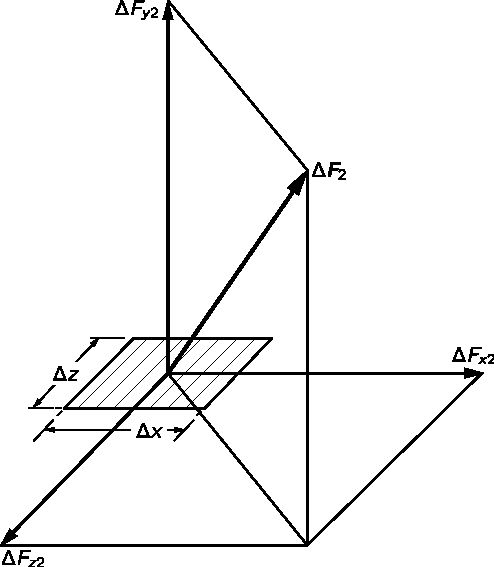
\includegraphics[width=0.8\linewidth]{fyz_fig0880.pdf}
      \caption{Síla působící na plošný element kolmý na \(y\) se rozkládá na tři navzájem kolmé
               složky (\cite[s.~584]{Feynman02})}
      \label{fyz:fig0880}
    \end{figure}

    Dále si představíme řez kolmý na osu \(y\). Na malou plošku \(\Delta x \Delta z\) působí síla
    \(Δ\vec{F_2}\). Opět rozložíme tuto sílu na tři složky tak, jak je to na obr. \ref{fyz:fig0880}.
    Z a definujeme tři složky napětí \(S_{xy}\), \(S_{yy}\), \(S_{zy}\) jako sílu působící na
    jednotkovou plochu ve třech směrech. Nakonec provedeme řez kolmo na \(z\) a definujeme tři
    složky \(S_{xz}\), \(S_{yz}\) a \(S_{zz}\). Máme tedy devět čísel:
    \begin{equation}\label{fyz:eq951}
      S_{ij}=
        \begin{bmatrix}
          S_{xx} & S_{xy} & S_{xz}  \\
          S_{yx} & S_{yy} & S_{yz}  \\
          S_{zx} & S_{zy} & S_{zz}  \\
        \end{bmatrix}.
    \end{equation}

    Nyní chceme ukázat, že těchto devět čísel stačí k úplnému popisu stavu vnitřního napětí a že
    \(S_{ij}\) je skutečně tenzorem. Předpokládejme, že chceme najít sílu působící na povrch pod
    nějakým libovolným úhlem. Můžeme ji určit z \(S_{ij}\)? Ano, můžeme, a to takovýmto způsobem:
    představme si malý, pevný hranol, jehož jedna stěna \(N\) je šikmá a ostatní dvě jsou rovnoběžné
    se souřadnicovými osami. Je-li stěna \(N\) rovnoběžná s osou \(z\), máme trojhranný útvar
    znázorněný na obr. \ref{fyz:fig0881}. (Je to trochu speciální případ, ale dostatečně ilustruje
    obecnou metodu.) Síly napětí působící na hranolek na obr. \ref{fyz:fig0881} jsou v rovnováze
    (přinejmenším v limitě nekonečně malých rozměrů), proto výsledná síla musí být rovna nule. Síly
    působící na stěny rovnoběžné se souřadnicovými osami zjistíme přímo z \(S_{ij}\). Jejich
    vektorový součet musí být roven síle působící na stěnu \(N\) takže tuto sílu umíme určit pomocí
    \(S_{ij}\).

    \begin{figure}[ht!] %\ref{fyz:fig0881}
      \centering
      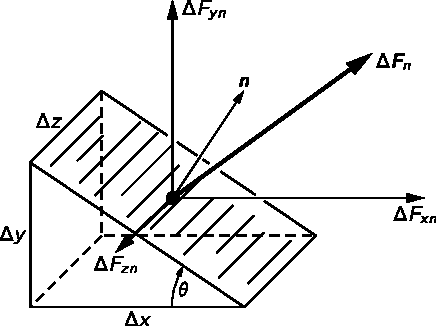
\includegraphics[width=0.8\linewidth]{fyz_fig0881.pdf}
      \caption{Síla\(\Delta F_n\) působící na plochu \(N\) (s jednotkovým vektorem \(\vec{n}\)) se
               rozkládá na tři složky (\cite[s.~585]{Feynman02})}
      \label{fyz:fig0881}
    \end{figure}

    Za našeho předpokladu, že \emph{plošné} síly působící na malý objem jsou v rovnováze,
    zanedbáváme všechny jiné \emph{objemové} síly, které by mohly být přítomny, například gravitaci
    nebo pseudosíly v případě, že naše souřadnicová soustava není inerciální soustavou. Všimněme si
    však, že takové objemové síly budou úměrné objemu hranolku, a tedy úměrné \(ΔxΔyΔz\), zatímco
    plošné síly jsou úměrné ploškám \(ΔxΔy\), \(ΔyΔz\) atd. Proto zvolíme-li si hranolek dostatečně
    malých rozměrů, budou objemové síly vždy zanedbatelné ve srovnání s plošnými silami.
    
    Nyní sečteme všechny síly působící na náš hranolek. Nejdříve vezměme složku \(x\), která je
    sumou pěti částí - po jedné z každé stěny. Je-li však \(Δz\) dostatečně malé, budou síly
    působící na trojúhelníkové stěny (kolmé na osu \(z\)) stejně velké a opačné, můžeme na ně tedy
    zapomenout. Složka \(x\) síly působící na spodní obdélník je
    \begin{equation*}
      \Delta F_{x2}=S_{xy}\,\Delta x\,\Delta z.
    \end{equation*}
    a \(x\)-ová složka síly působící na svislý obdélník je
    \begin{equation*}
      \Delta F_{x1}=S_{xx}\,\Delta y\,\Delta z.
    \end{equation*}
    Součet těchto dvou sil musí být roven \(x\)-ové složce síly působící na plochu \(N\) a směřující
    \emph{ven}. Nechť \(\vec{n}\) je jednotkový vektor kolmý na plochu \(N\) a \(\vec{F_n}\) nechť
    je síla působící na \(N\). Pak máme
    \begin{equation*}
      \Delta F_{xn}=S_{xx}\,\Delta y\,\Delta z+S_{xy}\,\Delta x\,\Delta z.
    \end{equation*}
    Složka \(S_{xn}\) napětí působícího na tuto plochu je rovna \(\Delta F_{xn}\) dělenému velikostí
    plochy \(\Delta z\sqrt{\Delta x^2+\Delta y^2}\), tj.
    \begin{equation*}
      S_{xn}=S_{xx}\,\frac{\Delta y}{\sqrt{\Delta x^2+\Delta y^2}}+
      S_{xy}\,\frac{\Delta x}{\sqrt{\Delta x^2+\Delta y^2}}.
    \end{equation*}
    Výraz \(\Delta x/\sqrt{\Delta x^2+\Delta y^2}\) je však kosinem úhlu \(\theta\) jenž svírají
    vektor \(\vec{n}\) a osa \(y\), jak to vidíme na obr. \ref{fyz:fig0881} - lze jej proto psát jako
    složkuy vektoru \(\vec{n}\), tj. jako \(n_y\). Podobně pro \(\Delta y/\sqrt{\Delta x^2+\Delta
    y^2}\) platí \(\sin\theta=n_x\). Můžeme psát
    \begin{equation*}
      S_{xn}=S_{xx}n_x+S_{xy}n_y.
    \end{equation*}
    Zobecníme-li to nyní na libovolný elementární povrch, dostaneme
    \begin{equation*}
      S_{xn}=S_{xx}n_x+S_{xy}n_y+S_{xz}n_z
    \end{equation*}
    nebo obecně
    \begin{equation}\label{fyz:eq952}
      S_{in}=\sum_jS_{ij}n_j.
    \end{equation} 
    Je tedy možné vyjádřit sílu působící na libovolnou elementární plochu pomocí koeficientů
    \(S_{ij}\), které tak úplně popisují vnitřní napětí v látce.

    \begin{figure}[ht!] %\ref{fyz:fig0882}
      \centering
      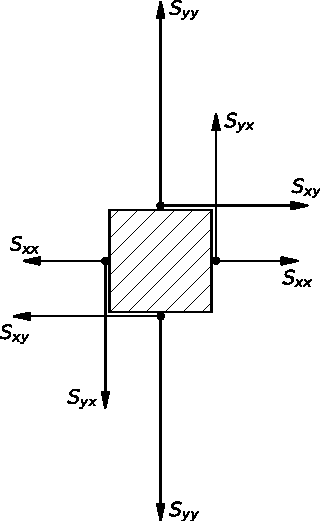
\includegraphics[width=0.7\linewidth]{fyz_fig0882.pdf}
      \caption{Složky sil \(x\) a \(y\) působících na čtyři stěny malé jednotkové krychle
               (\cite[s.~586]{Feynman02})}
      \label{fyz:fig0882}
    \end{figure}

    Rovnice \eqref{fyz:eq952} nám říká, že tenzor \(S_{ij}\) dává do vztahu sílu \(\vec{S_n}\) a
    jednotkový vektor \(\vec{n}\) právě tak, jako \(\alpha_{ij}\), dává do vztahu \(\vec{P}\) a
    \(\vec{E}\). Jelikož \(\vec{n}\) a \(\vec{S_n}\) jsou vektory, musí se složky \(S_{ij}\)
    transformovat při změně souřadnic jako tenzor. \(S_{ij}\) je tedy skutečně tenzorem.

    Jelikož \(S_{ij}\) je symetrickým tenzorem, může být popsán elipsoidem se třemi hlavními osami.
    Pro plochy kolmé na tyto osy jsou napětí obzvlášť jednoduchá - odpovídají tlaku nebo tahu
    kolmému na danou plochu. Podél těchto ploch nepůsobí žádné smykové síly. Pro \emph{libovolné}
    napětí můžeme vždy zvolit naše osy tak, aby byla smyková složka síly rovna nule. Je-li
    elipsoidem koule, působí v \emph{libovolném} směru jen kolmé složky. To odpovídá hydrostatickému
    tlaku (kladnému nebo zápornému). Pro hydrostatický tlak je tedy tenzor diagonální a všechny tři
    složky jsou navzájem rovny. Ve skutečnosti jsou rovny právě tlaku \(p\). Můžeme psát
    \begin{equation}\label{fyz:eq953}
      S_{ij}=p\delta_{ij}.
    \end{equation}

    Tenzor napětí, jakož i jeho elipsoid, se budou obecně měnit v dané látce od bodu k bodu.
    Chceme-li popsat daný kus látky, musíme udat hodnotu každé složky \(S_{ij}\) jako funkci polohy.
    Tenzor napětí je tedy \textbf{polem}. Poznali jsme už skalární pole, jako například teplotu
    \(T(x,y,z)\), v nichž je každému bodu v prostoru přiděleno jedno číslo, a vektorová pole jako
    \(\vec{E(x,y,z)}\), v nichž se každému bodu přiřazuje trojice čísel. Nyní máme tenzorové pole,
    kde je každému bodu prostoru přiřazeno devět čísel, nebo vlastně šest, protože \(S_{ij}\), je
    symetrický tenzor. Pro úplný popis vnitřních sil působících v libovolně deformované látce
    potřebujeme šest funkcí proměnných \(x, y, z\).
 
  \section{Tenzory vyššího řádu}\label{fyz:IIchapXXXIsecVII}
    
    Tenzor napětí \(S_{ij}\) popisuje \emph{vnitřní síly} v látce. Je-li látka elastická, je výhodné
    popisovat vnitřní \textbf{deformace} pomocí jiného tenzoru \(T_{ij}\), která se nazývá tenzor
    \emph{deformace}. Pro jednoduchý objekt, jako je například kovová tyč, umíme určit změnu délky
    \(ΔL\) podle \emph{Hookova zákona}, který říká, že prodloužení je přibližně úměrné síle:
    \begin{equation*}
      \Delta L=\gamma F.
    \end{equation*}
    
    Pro libovolné deformace pružného tuhého tělesa je vztah mezi deformací \(T_{ij}\) a napětím
    \(S_{ij}\) určen systémem lineárních rovnic 
    \begin{equation}\label{fyz:eq954}
      T_{ij}=\sum_{k,l}\gamma_{ijkl}S_{kl}.
    \end{equation}
    Také víme, že potenciální energie pružiny (nebo tyče) je rovna
    \begin{equation*}
      \dfrac{1}{2}F\,\Delta L=\dfrac{1}{2}\gamma F^2.
    \end{equation*}    
    Obecný výraz pro hustotu elastické energie pevného tělesa je
    \begin{equation}\label{fyz:eq955}
      U_{\text{elastic}}=\sum_{ijkl}\dfrac{1}{2}\gamma_{ijkl}S_{ij}S_{kl}.
    \end{equation}
    
    Úplný popis elastických vlastností krystalu je určen koeficienty \(\gamma_{ijkl}\). Tímto
    představujeme novou „obludu“ - \textbf{tenzor čtvrtého řádu}. Jelikož každý index může nabývat
    libovolnou ze tří hodnot \(x\), \(y\) nebo \(z\), dostáváme dohromady \(3^4 = 81\) koeficientů.
    Jenže ve skutečnosti je to jen 21 různých čísel. Zaprvé, jelikož tenzor \(S_{ij}\) je
    symetrický, obsahuje jen šest různých hodnot a v rovnici \eqref{fyz:eq955} potřebujeme jen 36
    \emph{různých} koeficientů. Zároveň však můžeme zaměnit \(S_{IJ}\) za \(S_{kl}\), aniž bychom
    změnili energii, proto \(\gamma_{ijkl}\) musí být symetrický při záměně \(ij\) za \(KL\). Tím se
    snižuje počet různých koeficientů na 21. Proto K popisu elastických vlastností krystalu s
    nejnižší možnou symetrií je třeba 21 elastických konstant! Tento počet je, samozřejmě, nižší pro
    krystaly s vyšší symetrií. Například krychlový krystal má jen tři pružné konstanty a izotropní
    látka má jen dvě.
    
    O správnosti předcházejícího tvrzení se můžeme přesvědčit. Jak mohou být složky tenzoru
    \(\gamma_{ijkl}\) nezávislé na směru os tak, jak to vyžadujeme pro izotropní látky? Odpověď je
    následující. Mohou být nezávislé \emph{jen} tehdy, když je lze vyjádřit pomocí tenzoru
    \(\delta_{ij}\). Existují dva možné výrazy \(\delta_{ij}\delta_{kl}\) a
    \(\delta_{ik}\delta_{jl}+\delta_{il}\delta_{jk}\) které mají požadovanou symetrii, proto
    \(\gamma_{ijkl}\) musí být jejich lineární kombinací. Proto pro izotropní látky platí
    \begin{equation*}
      \gamma_{ijkl}=a(\delta_{ij}\delta_{kl})+b(\delta_{ik}\delta_{jl}+\delta_{il}\delta_{jk}),
    \end{equation*}
    a potřebujeme dvě konstanty \(a\) a \(b\) k popisu elastických vlastností látky. Důkaz, že
    krychlový krystal potřebuje tři konstanty, přeskočíme.
    
    Jako poslední příklad, tentokrát na tenzor třetího řádu, uvádíme piezoelektrický efekt.
    Působením napětí se v krystalu vytváří elektrické pole úměrné napětí. Obecný zákon má tvar
    \begin{equation*}
      E_i=\sum_{j,k}P_{ijk}S_{jk},
    \end{equation*}
    kde \(E_i\) je elektrické pole a \(P_{ijk}\) jsou piezoelektrické koeficienty nebo
    piezoelektrický tenzor. Uměli bychom dokázat, že má-li krystal střed inverze (invariance při
    záměně \(x,y,z\to-x,-y,-z\) všechny piezoelektrické koeficienty jsou rovny nule?

  \section{Čtyřtenzor elektromagnetické energie a hybnosti}\label{fyz:IIchapXXXIsecVIII} 
    Všechny tenzory, které jsme v této kapitole dosud probírali, se vztahují k trojrozměrnému
    prostoru. Jsou definovány jako veličiny, které mají určité transformační vlastnosti při
    trojrozměrných rotacích. V kapitole \ref{fyz:IIchapXXVI} jsme měli možnost pracovat s tenzorem
    ve \emph{čtyřrozměrném relativistickém časoprostoru}, a to s tenzorem elektromagnetického pole
    \(F_{\mu\nu}\). Složky takového čtyřtenzoru se při Lorentzově transformaci souřadnic
    transformují určitým způsobem, který jsme odvodili. (Ačkoli jsme to tak nedělali, mohli jsme
    Lorentzovy transformace považovat za „rotace“ ve čtyřrozměrném „prostoru“, který se nazývá
    \emph{Minkowského prostor}. Pak by i analogie s tím, co nyní děláme, byla jasnější.)
    
    Jako náš poslední příklad zmíníme ještě jeden čtyřrozměrný tenzor z teorie relativity. Když jsme
    hovořili o tenzoru napětí, definovali jsme \(S_{ij}\) jako složky sil působících na jednotlivé
    plochy. Ale síla je rovna časové změně hybnosti. Proto místo výroku „\(S_{xy}\) je složkou \(x\)
    síly působící na jednotkovou plochu kolmou na \(y\)“ bychom stejně správně mohli říci
    „\(S_{xy}\) je rychlost změny toku složky \(x\) hybnosti jednotkovou plochou kolmou na \(y\).
    Jinými slovy, každá složka \(S_{ij}\) představuje i hustotu toku \(i\)-té složky hybnosti
    jednotkovou plochou kolmou na směr \(j\). Tyto čistě prostorové složky jsou však součástí
    „většího“ tenzoru \(S_{\mu\nu}\) ve čtyřech rozměrech (\(\mu\) a \(v= t, x,y,z\), který obsahuje
    navíc složky typu \(S_{xx}\), \(S_{xy}\), a \(S_{xz}\) atd. Nyní se pokusíme najít fyzikální
    význam těchto dodatečných složek.
    
    Víme, že prostorové složky představují hustotu toku hybnosti. Klíč k interpretaci časové složky
    nám poskytne jiný druh „toku“ - tok elektrického náboje. Rychlosti toku \emph{skalární}
    veličiny, náboje (jednotkovou plochou kolmou na tok), přiřazujeme prostorový vektor - vektor
    proudové hustoty \(\vec{j}\). Viděli jsme, že časová složka tohoto vektoru toku představuje
    hustotu toho, co teče. Například \(\vec{j}\) můžeme kombinovat s hustotou náboje \(\varrho\) a
    dostaneme čtyřvektor \(j_\mu=(\varrho,\vec{j})\) tj. index \(\mu\) v \(i_\mu\) nabývá hodnoty
    \(t\), \(x\), \(y\), \(z\), což postupně označuje hustotu, hustotu toku ve směru \(x\), hustotu
    toku ve směru \(y\) hustotu toku ve směru \(z\) skalárního náboje.
    
    Nyní, v analogii s naším tvrzením o časové složce toku skalární veličiny, bychom mohli očekávat,
    že vedle \(S_{xx}\), \(S_{xy}\), a \(S_{xz}\), které popisují tok \(x\)-ové složky hybnosti,
    existuje i časová složky \(S_{xt}\), která představuje hustotu toho, co teče, tj. \(S_{xt}\) by
    měla být hustotou \(x\)-ové složky hybnosti. Náš tenzor tak můžeme horizontálně rozšířit o
    složku \(t\). Dostaneme:
    \begin{itemize}[noitemsep]
      \item \(S_{xt}\ldots\) hustota \(x\)-ové složky hybnosti,
      \item \(S_{xx}\ldots\) hustota toku \(x\)-ové složky hybnosti ve směru \(x\),
      \item \(S_{xy}\ldots\) hustota toku \(x\)-ové složky hybnosti ve směru \(y\),
      \item \(S_{xz}\ldots\) hustota toku \(x\)-ové složky hybnosti ve směru \(z\).
    \end{itemize}
    Podobně pro \(y\)-ovou složku hybnosti máme tři složky hustoty toku \(S_{yx}\), \(S_{yy}\),
    \(S_{yz}\), k nimž přidáme čtvrtou složku
    
    \begin{center}
      \(S_{yt}\) = hustota \(y\)-ové složky hybnosti.
    \end{center}

    A samozřejmě, k \(S_{zz}\) bychom měli přidat
    \begin{center}
      \(S_{zt}\) = hustota \(z\)-ové složky hybnosti.
    \end{center}
    
    Ve čtyřech rozměrech existuje i složka \(t\) hybnosti, a to je, jak víme, energie. Proto by
    tenzor \(S_{ij}\) měl být rozšířen i vertikálně o složky \(S_{tx}\), \(S_{ty}\), a \(S_{tz}\)
    kde
    \begin{itemize}[noitemsep]
      \item \(S_{tx}\ldots\) hustota toku energie ve směru \(x\),
      \item \(S_{ty}\ldots\) hustota toku energie ve směru \(y\),
      \item \(S_{tz}\ldots\) hustota toku energie ve směru \(z\).
    \end{itemize}
    tj. \(S_{tx}\) je tok energie jednotkovou plochou kolmou k ose \(x\) na jednotku času atd.
    Nakonec, abychom zkompletovali náš tenzor, potřebujeme \(S_{tt}\) a to by měla být
    \textbf{hustota energie}. Náš trojrozměrný tenzor napětí \(S_{ij}\) jsme tak rozšířili na
    \textbf{čtyřrozměrný tenzor energie a hybnosti} \(S_{\mu\nu}\). Index \(\mu\) může nabývat čtyř
    hodnot \(t\), \(x\), \(y\), \(z\), které postupně označují hustotu, hustotu toku ve směru \(x\)
    hustotu toku ve směru \(y\) a hustotu toku ve směru \(z\). Podobně \(\nu\) nabývá čtyř hodnot
    \(t\), \(x\), \(y\), \(z\), které označují to, \emph{co} teče: energii, hybnost ve směru \(x\)
    hybnost ve směru \(y\) a hybnost ve směru \(z\).
    
    Jako příklad budeme tento tenzor uvažovat ne v látce, ale v nějaké oblasti volného prostoru, kde
    působí elektromagnetické pole. Víme, že hustota toku energie je určena \emph{Poyntingovým
    vektorem} \(\vec{S}=\epsilon_0c^2\vec{E}\times\vec{B}\). Z relativistického hlediska jsou složky
    \(x\), \(y\), \(z\) vektoru \(\vec{S}\) složkami \(S_{tx}\), \(S_{ty}\), a \(S_{tz}\) našeho
    čtyřrozměrného tenzoru energie a hybnosti. Symetrie tenzoru \(S_{ij}\) platí stejně i pro časové
    složky, proto je čtyřrozměrný tenzor \(S_{\mu\nu}\) symetrický
    \begin{equation}\label{fyz:eq956}
      S_{\mu\nu}=S_{\nu\mu}.
    \end{equation}
    Jinými slovy, složky \(S_{xt}\), \(S_{yt}\), \(S_{zt}\), které představují hustoty složek \(x\),
    \(y\) a \(z\) hybnosti, jsou zároveň složkami \(x\), \(y\) a \(z\) Poyntingova vektoru
    \(\vec{S}\), který představuje hustotu toku energie, jak jsme už ukázali v jedné z
    předcházejících kapitol.
    
    Zbývající složky elektromagnetického tenzoru energie a hybnosti \(S_{\mu\nu}\) lze také vyjádřit
    pomocí elektrického a magnetického pole \(\vec{E}\) a \(\vec{B}\). Musíme tedy připustit
    existenci napětí nebo, aby to neznělo tak záhadně, existenci toku hybnosti v elektromagnetickém
    poli. Mluvili jsme o tom v kapitole \ref{fyz:IIchapXXVII} v souvislosti s rovnicí
    \eqref{fyz:eq957}, ale tehdy jsme nešli do detailů.
    
    Chceme-li si vyzkoušet svou zručnost v zacházení s tenzory ve čtyřech rozměrech, je dobré
    vědět, jak \(S_{\mu\nu}\) vyjádřit pomocí polí:
    \begin{equation*}
      S_{\mu\nu}=-\varepsilon_0\biggl(
      \sum_\alpha F_{\mu\alpha}F_{\nu\alpha}-\dfrac{1}{4}\delta_{\mu\nu}
      \sum_{\alpha,\beta}F_{\beta\alpha}F_{\beta\alpha}
      \biggr),
    \end{equation*}
    kde sčítání přes \(\alpha\), \(\beta\) znamená sčítání přes \(t\), \(x\), \(y\), \(z\), ale (jak
    to bývá zvykem v teorii relativity) sumační znak \(\sum\) a symbol \(\delta\) mají speciální
    význam. Při sumaci se členy s \(x\), \(y\), \(z\) odčítají a \(δ_{tt}=+1\), zatímco \(δ_{xx} =
    δ_{yy} = δ_{zz}= −1\) a \(δ_{μ\nu}=0\) pro \(μ≠ν\) (\(c=1\)). Uměli bychom ověřit, že toto
    vyjádření vede k hustotě energie \(S_{tt}=(\varepsilon_0/2)\,(E^2+B^2)\) a k Poyntingovu vektoru
    \(\varepsilon_0\vec{E}\times\vec{B}\)? Uměli bychom ukázat, že v elektrostatickém poli, kde
    \(\vec{B}= 0\), mají hlavní osy napětí směr elektrického pole a že ve směru pole vzniká napětí
    \((\varepsilon_0/2)E^2\), zatímco ve směru kolmém na pole vzniká stejně velký \emph{tlak}?  
  % % !TeX spellcheck = cs_CZ
%{\tikzset{external/prefix={tikz/FYZII/}}
% \tikzset{external/figure name/.add={ch10_}{}}
%---------------------------------------------------------------------------------------------------
% file fey2ch10.tex
%---------------------------------------------------------------------------------------------------
%=========================== Kapitola: Dielektrika =================================================
\setchaptertoc
\chapter{Dielektrika}\label{fyz:IIchapX}
  \section{Permitivita}\label{fyz:IIchapXsecI}
    Na tomto místě začneme hovořit o další z charakteristických vlastností látky nacházející se pod
    vlivem elektrického pole. V jedné z předcházejících kapitol jsme se zabývali vlastnostmi
    \emph{vodičů}, v nichž se účinkem elektrického pole náboje volně přemisťují do takových míst, že
    uvnitř vodiče nezůstane žádné pole. Nyní budeme hovořit o \emph{izolantech}, tedy o látkách,
    které elektřinu nevedou. Na první pohled by se mohlo zdát, že se s nimi v elektrickém poli
    nestane vůbec nic. Ale Faraday pomocí jednoduchého elektroskopu a deskového kondenzátoru
    objevil, že tomu tak není. Jeho pokusy ukázaly, že kapacita takového kondenzátoru
    \emph{vzroste}, když se mezi jeho elektrody vloží izolant. Vyplní-li izolant prostor mezi
    elektrodami, kapacita se zvětší \(\varepsilon_r\)-krát, přičemž koeficient \(\varepsilon_r\)
    závisí pouze na vlastnostech izolační látky. Izolační látky se také nazývají \emph{dielektrika};
    součinitel \(\varepsilon_r\) je tedy vlastností dielektrika a nazývá se \emph{relativní
    permitivita}. Relativní permitivita vakua je, samozřejmě, rovna jedné.  

    Naší úlohou je nyní vysvětlit, proč vůbec nějaký elektrický efekt nastává, jsou-li izolanty
    opravdu izolanty a elektřinu nevedou. Vyjdeme z experimentálního faktu, že kapacita vzrůstá a
    pokusíme se vymyslet, co by se přitom mohlo dít. Uvažujme deskový kondenzátor s nějakými náboji
    na povrchu vodičů, řekněme se záporným nábojem na horní a s kladným nábojem na dolní elektrodě.
    Předpokládejme, že vzdálenost mezi elektrodami je \(d\) a plošný obsah každé elektrody je \(S\).
    Jak jsme viděli už dříve, kapacita kondenzátoru je
    \begin{equation}\label{fyz:eq907}
      C = \dfrac{\varepsilon_0S}{d}
    \end{equation}
    a náboj souvisí s napětím na kondenzátoru podle vztahu
    \begin{equation}\label{fyz:eq908}
      Q = CU.
    \end{equation}

    Experimentálním faktem je, že vložíme-li mezi desky kus izolantu, například skla nebo plexiskla,
    zjistíme, že se kapacita zvětší. To ovšem znamená, že při témže náboji se napětí snížilo. Ale
    napětí je integrálem elektrického pole počítaným napříč kondenzátorem; musíme tedy udělat závěr,
    že uvnitř kondenzátoru se zeslabilo elektrické pole, i když náboje na deskách zůstávají
    nezměněny.

    \begin{figure}[ht!] %\ref{fyz:fig0705}
      \centering
      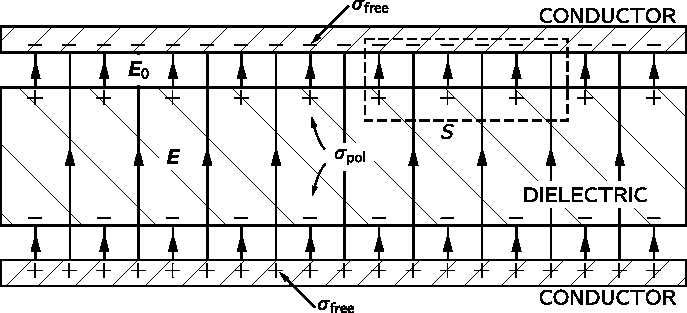
\includegraphics[width=0.9\linewidth]{fyz_fig0705.pdf}
      \caption{Deskový kondenzátor s dielektrikem. Vyznačeny jsou siločáry elektrického pole \(E\).
               (\cite[s.~175]{Feynman02})}
      \label{fyz:fig0705}
    \end{figure}

    Jak je to možné? Máme větu, pocházející od Gausse, která nám říká, že tok elektrického pole
    uzavřenou plochou je v přímém vztahu s náboji uvnitř plochy. Uvažujme gaussovskou plochu \(S\)
    vyznačenou na obr. \ref{fyz:fig0705} čárkovaně. Protože elektrické pole se v přítomnosti
    dielektrika zeslabilo, usuzujeme, že celkový náboj uvnitř plochy musí být menší, než byl bez
    látky. Pak existuje jediný možný závěr a ten je, že na povrchu dielektrika musí sídlit kladné
    náboje. Protože se sice pole zeslabilo, ale ne na nulu, očekáváme, že tento kladný náboj je
    menší než záporný náboj na vodiči. Celý úkaz by bylo možné vysvětlit, kdybychom nějak uměli
    pochopit, proč se při umístění dielektrické látky do elektrického pole na jednom povrchu
    indukuje kladný a na druhém záporný náboj.

    Něco takového bychom očekávali v případě vodiče. Mějme například kondenzátor se vzdáleností
    \(d\) mezi elektrodami a vložme mezi ně neutrální vodič, jehož tloušťka je \(b\) (obr.
    \ref{fyz:fig0706}). Elektrické pole indukuje kladný náboj na jeho horním povrchu a záporný náboj
    na jeho dolním povrchu, takže uvnitř vodiče pole není. Ve zbývajícím prostoru je pole totéž,
    jako by bylo bez vodiče, neboť je rovno plošné hustotě náboje dělené \(\varepsilon_0\) ale
    vzdálenost, přes kterou musíme integrovat, abychom dostali napětí (rozdíl potenciálů), se
    zmenšila.

    Napětí je
    \begin{equation*}
      U = \dfrac{U}{\varepsilon_0}(d-b).
    \end{equation*}
    Výsledný výraz pro kapacitu je stejný jako (\ref{fyz:eq907}), ale \(d\) je nahrazeno rozdílem
    \((d - b)\)
    \begin{equation}\label{fyz:eq909}
      C = \dfrac{\varepsilon_0S}{d\left[1 - (b/d)\right]}
    \end{equation}
    Kapacita se zvětšila v poměru, jenž závisí na \((b/d)\), tj. na poměrné části objemu, kterou
    zaujal vodič.

    \begin{figure}[ht!] %\ref{fyz:fig0706}
      \centering
      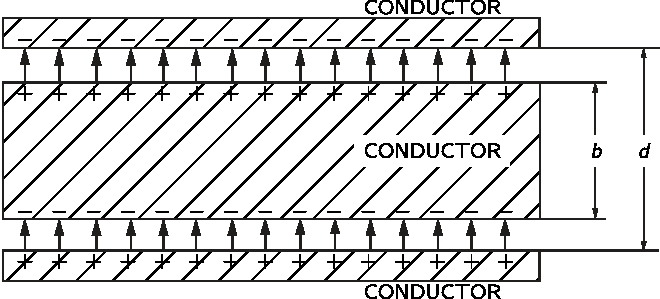
\includegraphics[width=0.9\linewidth]{fyz_fig0706.pdf}
      \caption{Vložíme-li mezi elektrody deskového kondenzátoru vodivou desku, indukované náboje
               zeslabí pole uvnitř vodiče na nulovou hodnotu. (\cite[s.~175]{Feynman02})}
      \label{fyz:fig0706}
    \end{figure}

    To nám však poskytuje zřejmý model toho, co se děje s dielektriky - uvnitř látky se nachází
    množství tenkých vodivých vrstev. S takovým modelem je však spojena jedna obtíž - má významnou
    osu, normálu k vrstvám, zatímco většina dielektrik takovou osu nemá. Ale tuto obtíž je možno
    vyloučit, uděláme-li předpoklad, že všechny izolační látky obsahují malé navzájem izolované
    vodivé koule, jak ukazuje obr. \ref{fyz:fig0707}. Permitivita je vysvětlována působením nábojů,
    které by byly indukovány na každé kuličce. Je to jeden z prvních fyzikálních modelů dielektrika,
    použitých na vysvětlení jevu pozorovaného Faradayem. Konkrétněji řečeno, předpokládalo se, že
    každý z atomů látky je dokonalým vodičem, ale izolovaným od jiných atomů. Relativní permitivita
    \(\varepsilon_0\) bude záviset na tom, jakou část objemu zabírají vodivé koule. Dnes však tento
    model nepoužíváme.

    \begin{figure}[ht!] %\ref{fyz:fig0707}
      \centering
      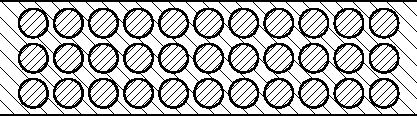
\includegraphics[width=0.9\linewidth]{fyz_fig0707.pdf}
      \caption{Model dielektrika: malé vodivé kuličky zapuštěné do idealizovaného izolátoru
               (\cite[s.~176]{Feynman02})}
      \label{fyz:fig0707}
    \end{figure}

  \section{Vektor elektrické polarizace P}\label{fyz:IIchapXsecII} 
    Pokračujeme-li v naší analýze, přijdeme na to, že představa o oblastech s dokonalou vodivostí a
    izolací mezi nimi není podstatná. Každá z malých kuliček se chová jako dipól, jehož moment je
    indukován vnějším polem. Jediná věc, jež je pro pochopení dielektrik podstatná je ta, že v
    dielektrické látce je indukováno mnoho malých dipólů. To, zda se dipóly indukují proto, že
    existují vodivé malé kuličky, nebo z nějakého jiného důvodu, je bezvýznamné.

    Proč by pole mělo v atomu indukovat dipólový moment, není-li atom vodivou koulí? O této otázce
    budeme mluvit mnohem podrobněji v následující kapitole, která bude věnována vnitřním procesům v
    dielektrických látkách. Zde však uvedeme jeden příklad, abychom ilustrovali možný mechanizmus.
    Kladný náboj atomu je v jádře, jež je obklopeno zápornými elektrony. Orbity nebo vlnové balíky
    elektronů (nebo jakékoliv zobrazení použité v kvantové mechanice) jsou v nějaké míře pokřiveny
    (obr. \ref{fyz:fig0708}); těžiště záporného náboje se posune a nebude už splývat s kladným
    nábojem jádra. My jsme už o takovém rozdělení náboje hovořili. Díváme-li se na něj z velké
    vzdálenosti, je taková neutrální konfigurace v prvním přiblížení ekvivalentní malému dipólu.

    \begin{figure}[ht!]
      \centering
      \subcaptionbox{\label{fyz:fig0708a}}{\luafigure[0.45]{fyz_fig0708a.pdf}}
      \subcaptionbox{\label{fyz:fig0708b}}{\luafigure[0.45]{fyz_fig0708b.pdf}}
      \caption{Rozdělení elektronů v atomu nacházejícím se v elektrickém poli se vzhledem k jádru
              posune. (\cite[s.~177]{Feynman02})}
      \label{fyz:fig0708}
    \end{figure}

    Asi je rozumné předpokládat, že není-li pole příliš silné, velikost indukovaného dipólového
    momentu bude přímo úměrná poli. Slabé pole tedy posune náboje jen o malý kousíček, zatímco silné
    pole je posune víc, a to přímo úměrně poli, jen když posunutí nebude příliš velké. Do konce této
    kapitoly budeme dipólový moment považovat za přesně přímo úměrný poli.

    Dále budeme předpokládat, že v každém atomu jsou náboje \(q\) ve vzájemné vzdálenosti
    \(\vec{δ}\) takže \(q\vec{δ}\) je elektrický dipólový moment připadající na jeden atom.
    (\(\vec{δ}\) používáme proto, neboť \(d\) jsme už použili pro vzdálenost elektrod.) Je-li v
    jednotkovém objemu \(N\) atomů, bude \textbf{dipólový moment jednotkového objemu} roven
    \(Nq\vec{δ}\). Tento elektrický dipólový moment připadající na jednotkový objem budeme označovat
    vektorem \(\vec{P}\). Není třeba zdůrazňovat, že leží ve směru jednotlivých dipólových momentů,
    tj. ve směru posunutí nábojů \(\vec{δ}\).
    \begin{equation}\label{fyz:eq910}
      \vec{P} = Nq\vec{δ}
    \end{equation}

    Obecně se bude \(\vec{P}\) v dielektriku měnit od místa k místu. Ale v každém bodě látky je
    přímo úměrné elektrickému poli. Součinitel této úměrnosti je určen tím, jak snadno se elektron
    posune, a závisí na druhu atomů v látce.
    
    O tom, co doopravdy určuje, jak se tento součinitel chová, jak přesně konstantní je ve velmi
    silných polích a co se děje uvnitř různých látek, budeme mluvit později. V této chvíli budeme
    prostě předpokládat, že existuje mechanizmus, jímž se indukuje elektrický dipólový moment přímo
    úměrný elektrickému poli.

  \section{Polarizační náboje}\label{fyz:IIchapXsecIII}   
    Nyní prozkoumejme, co z tohoto modelu vyplývá pro teorii kondenzátoru vyplněného dielektrikem.
    Nejdříve uvažujeme destičku z látky, která má určitý elektrický dipólový moment připadající na
    jednotkový objem. Vznikne v důsledku toho v průměru nějaká hustota náboje v látce? Ne, je-li
    \(\vec{P}\) homogenní. Mají-li kladné a záporné náboje po posunutí stejné hustoty náboje, z
    jejich posunutí nevzniká v objemu žádný výsledný náboj. Na druhé straně, kdyby \(\vec{P}\) bylo
    v jednom místě větší a v druhém místě menší, znamenalo by to, že se do některé oblasti přesunulo
    více náboje, než se z ní vysunulo ven; tehdy bychom mohli očekávat nenulovou objemovou hustotu
    náboje. V případě deskového kondenzátoru předpokládáme, že \(\vec{P}\) je homogenní, takže je
    nutné prozkoumat pouze to, co se děje na povrchu. Na jednom povrchu se záporné náboje -
    elektrony efektivně vysunuly do vzdálenosti \(δ\), zatímco na druhém povrchu se posunuly dovnitř
    a zanechaly určitý kladný náboj na vzdálenosti \(δ\). Jak ukazuje obr. \ref{fyz:fig0709}, na
    povrchu vznikne plošná hustota náboje, který budeme nazývat \textbf{povrchovým polarizačním
    nábojem}.

    Tento náboj je možné vypočítat následujícím způsobem. Počet elektronů, které se objeví na
    povrchu destičky je roven součinu jejího plošného obsahu \(S\), počtu elektronů v jednotkovém
    objemu \(N\) a posunutí \(δ\), o němž zde předpokládáme, že nastane kolmo k povrchu. Výsledný
    náboj dostaneme vynásobením této hodnoty nábojem elektronu \(q_e\). Abychom dostali plošnou
    hustotu polarizačního náboje indukovaného na povrchu, musíme výsledek dělit plošným obsahem
    \(S\). Velikost plošné hustoty náboje tedy bude
    \begin{equation*}
      σ_{\text{pol}}=Nq_eδ.
    \end{equation*}
    To je však právě rovno velikosti \(P\) vektoru elektrické polarizace \(\vec{P}\), daného vztahem
    (\ref{fyz:eq910}), tj. 
    \begin{equation}\label{fyz:eq911}
      σ_{\text{pol}} = P.
    \end{equation}
    \emph{Plošná hustota náboje na povrchu látky je rovna elektrické polarizaci v jejím vnitřku.}
    Povrchový náboj je samozřejmě kladný na jedné straně a záporný na opačné straně povrchu.

    \begin{figure}[ht!] %\ref{fyz:fig0709}
      \centering
      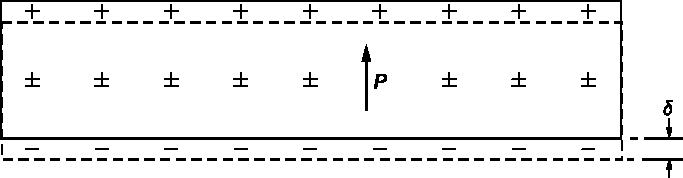
\includegraphics[width=1\linewidth]{fyz_fig0709.pdf}
      \caption{Dielektrická vrstva v homogenním poli. Kladné náboje jsou posunuty do vzdálenosti
              \(δ\) vzhledem k záporným. (\cite[s.~177]{Feynman02})}
      \label{fyz:fig0709}
    \end{figure}
    
    Dále předpokládejme, že naše deska představuje dielektrikum v rovinném kondenzátoru. Na
    \emph{elektrodách} kondenzátoru se také nachází plošný náboj, jehož hustotu označíme
    \(σ_{\text{free}}\), neboť ve vodiči se náboje mohou „volně“ pohybovat. Jde, samozřejmě, o
    náboj, který jsme dodali při nabíjení kondenzátoru. Je nutné zdůraznit, že \(σ_{\text{pol}}\)
    existuje jen proto, že existuje \(σ_{\text{free}}\). Odstraní-li se vybitím kondenzátoru
    \(σ_{\text{free}}\), vymizí také \(σ_{\text{pol}}\). Neodejde však vodičem, kterým se vybije
    kondenzátor, ale pohybem zpět dovnitř látky, a to rozptýlením polarizace uvnitř látky.

    Nyní můžeme na gaussovskou plochu \(S\), znázorněnou na obr. \ref{fyz:fig0705}, použít Gaussův
    zákon. Elektrické pole \(\vec{E}\) v dielektriku je rovno celkové plošné hustotě náboje dělené
    \(\varepsilon_0\). Je zřejmé, že \(σ_{\text{pol}}\) a \(σ_{\text{free}}\) mají opačná znaménka,
    takže
    \begin{equation}\label{fyz:eq912}
      E = \dfrac{σ_{\text{free}} - σ_{\text{pol}}}{\varepsilon_0}.
    \end{equation}

    Všimněme si, že pole \(E_0\) mezi kovovou elektrodou a povrchem dielektrika je větší než pole
    \(E\); odpovídá pouze hustotě \(σ_{\text{free}}\). Zde se však zajímáme o pole uvnitř
    dielektrika. Vyplňuje-li dielektrikum téměř celou mezeru mezi elektrodami, je toto pole
    rozprostřeno prakticky v celém objemu uvnitř kondenzátoru. Použijeme-li vztah (\ref{fyz:eq911}),
    můžeme napsat
    \begin{equation}\label{fyz:eq913}
      E = \dfrac{σ_{\text{free}} - P}{\varepsilon_0}.
    \end{equation}
    Z této rovnice se nemůžeme dovědět, jaké je elektrické pole, bez znalosti \(P\). Zde však
    předpokládáme, že \(P\) závisí na \(E\), konkrétně, že je přímo úměrné \(E\). Tato přímá
    úměrnost se obvykle zapisuje takto:
    \begin{equation}\label{fyz:eq914}
      \vec{P}=χ\varepsilon_0\vec{E}.
    \end{equation}
    Konstanta \(χ\) (řecké „chí“) se nazývá \textbf{elektrická susceptibilita dielektrika}.

    Potom vztah (\ref{fyz:eq913}) nabude tvaru
    \begin{equation}\label{fyz:eq915}
      E=\dfrac{σ_{\text{free}}}{\varepsilon_0}\dfrac{1}{(1+χ)},
    \end{equation}
    podle kterého se pole zmenšilo v poměru \(1/(1+χ)\).

    Napětí mezi elektrodami vyjadřuje integrál elektrického pole. Protože jde o homogenní pole,
    integrál je redukován na součin intenzity pole \(E\) a vzdálenosti \(d\) mezi elektrodami.
    Dostáváme
    \begin{equation*}
      U = Ed = \dfrac{σ_{\text{free}}d}{\varepsilon_0(1+χ)}
    \end{equation*}

    Celkový náboj na kondenzátoru je \(C = σ_{\text{free}}S\) takže pro kapacitu definovanou vztahem
    (\ref{fyz:eq908}) dostaneme vyjádření
    \begin{equation}\label{fyz:eq916}
      C=\dfrac{\varepsilon_0S(1+χ)}{d} = \dfrac{\varepsilon_r\varepsilon_0S}{d}.
    \end{equation}

    Vysvětlili jsme pozorovaná fakta. Vyplníme-li rovinný deskový kondenzátor dielektrikem, vzroste
    jeho kapacita \(\varepsilon_r\)-krát, přičemž
    \begin{equation}\label{fyz:eq917}
      \varepsilon_r = 1+χ
    \end{equation}
    charakterizuje vlastnosti látky. Je pravda, že naše vysvětlení nebude úplné, dokud nevysvětlíme
    (uděláme to později), jak dochází k polarizaci atomů.

    \begin{figure}[ht!] %\ref{fyz:fig0710}
      \centering
      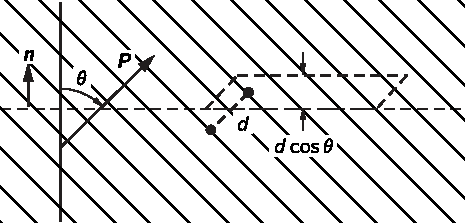
\includegraphics[width=0.9\linewidth]{fyz_fig0710.pdf}
      \caption{Náboj, který prošel v dielektriku elementární myšlenou ploškou, je přímo úměrný
               složce vektoru \(\vec{P}\) ve směru normály k ploše. (\cite[s.~179]{Feynman02})}
      \label{fyz:fig0710}
    \end{figure}

    Zabývejme se nyní něčím trochu složitějším - případem, kdy elektrická polarizace \(\vec{P}\)
    není všude stejná. Jak jsme již řekli, není-li polarizace konstantní, je možné obecně očekávat
    nenulovou objemovou hustotu náboje, protože z jedné strany může do malého objemového elementu
    vejít více náboje, než z něj může na druhé straně vyjít. Jak zjistíme, kolik náboje do malého
    objemu přibylo nebo se z něj ztratilo? Nejdříve vypočtěme, jaký náboj projde myšlenou plochou
    při polarizaci látky. V případě, že polarizace má směr normály k ploše, množství náboje
    procházející plochou je rovno součinu P a obsahu plochy. Samozřejmě, když má polarizace směr
    tečny k ploše, neprochází plochou žádný náboj.

    Týmiž úvahami, které jsme již provedli, se snadno přesvědčíme, že náboj, jenž projde libovolným
    plošným elementem, je přímo úměrný \emph{složce vektoru \(\vec{P}\) kolmé na plochu}. Porovnejme
    obr. \ref{fyz:fig0710} s obr. \ref{fyz:fig0709}. Vidíme, že vztah (\ref{fyz:eq911}) je nutné
    obecně psát takto:
    \begin{equation}\label{fyz:eq918}
      σ_{\text{pol}}=\vec{P}\cdot\vec{n}.
    \end{equation}

    Máme-li na mysli plošný element uvnitř dielektrika, udává vztah (\ref{fyz:eq918}) náboj, který
    prošel plochou, ale nevede k vzniku plošného náboje, neboť příspěvky od dielektrika jsou po obou
    stranách plochy stejné a mají opačná znaménka.

    \begin{figure}[ht!] %\ref{fyz:fig0711}
      \centering
      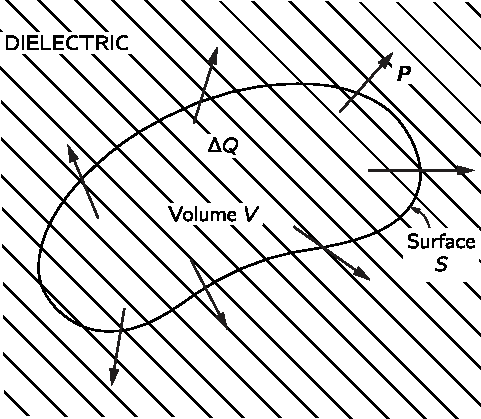
\includegraphics[width=0.9\linewidth]{fyz_fig0711.pdf}
      \caption{Nehomogenní polarizace \(\vec{P}\) může vést ke vzniku náboje v objemu dielektrika.
               (\cite[s.~707]{Feynman02})}
      \label{fyz:fig0711}
    \end{figure}

    Posunutí nábojů však mohou vést ke vzniku objemové hustoty náboje. Celkový náboj vysunutý
    polarizací ven z néjakého objemu \(V\) je roven integrálu normálové složky vektoru \(\vec{P}\)
    plochou \(S\), která ohraničuje \(V\) (obr. \ref{fyz:fig0711}). Stejně velký přebytek náboje
    opačného znaménka zůstane uvnitř. Označíme-li jej \(ΔQ_{\text{pol}}\), bude platit
    \begin{equation}\label{fyz:eq919}
      \Delta Q_{\text{pol}}=-\int_S\vec{P}\cdot\vec{n}\dd{S}.
    \end{equation}
    \(\Delta Q_{\text{pol}}\) můžeme vyjádřit pomocí objemového rozdělení náboje s hustotou
    \(ρ_{\text{pol}}\)
    \begin{equation}\label{fyz:eq920}
      \Delta Q_{\text{pol}}=\int_V\rho_{\text{pol}}\dd{V}.
    \end{equation}
    Z rovnosti pravých stran obou těchto výrazů vyplývá
    \begin{equation}\label{fyz:eq921}
      \int_V\rho_{\text{pol}}\dd{V}=-\int_S\vec{P}\cdot\vec{n}\dd{S}.
    \end{equation}
    Dostali jsme něco jako Gaussovu větu, která uvádí do souvislosti hustotu náboje v polarizovaných
    látkách a vektor elektrické polarizace \(vec{P}\). Můžeme se přesvědčit, že souhlasí s
    výsledkem, který jsme dostali pro povrchový polarizační náboj nebo pro dielektrikum v deskovém
    kondenzátoru. Aplikujeme-li rovnici (\ref{fyz:eq921}) na gaussovskou plochu z obr.
    \ref{fyz:fig0705}, bude plošný itegrál roven \(PΔS\) a náboj uvnitř plochy bude
    \(\sigma_{\text{pol}}\,\Delta S\), takže opět dostáváme \(σ_{\text{pol}}=P\).
    
    Stejně jako v případě elektrostatického Gaussova zákona můžeme i rovnici (\ref{fyz:eq921})
    transformovat na diferenciální tvar použitím Gaussovy věty z matematiky:
    \begin{equation*}
      \int_S\vec{P}\cdot\vec{n}\dd{S}=\int_V∇\cdot\vec{P}\dd{V}.
    \end{equation*}
    Dostaneme
    \begin{equation}\label{fyz:eq922}
      ρ_{\text{pol}}=−∇⋅\vec{P}.
    \end{equation}
    Je-li polarizace nehomogenní, dává její divergence výslednou hustotu náboje vznikající v látce.
    Zdůrazňujeme, že jde o naprosto \emph{reálnou} hustotu náboje; „polarizačním nábojem“ jej
    nazýváme proto, abychom připomněli, odkud se vzal.

  \section{Elektrostatické rovnice pro dielektrika}\label{fyz:IIchapXsecIV}
    Nyní už spojme uvedený výsledek s naší elektrostatickou teorií. Základní rovnice je
    \begin{equation}\label{fyz:eq936}
      ∇\cdot\vec{E}=\dfrac{\varrho}{\varepsilon_0}.
    \end{equation}
    kde \(ρ\) je hustota všech elektrických nábojů. Protože není snadné sledovat polarizační náboje,
    je vhodné rozdělit \(ρ\) na dvě části. Opět budeme jako \(ρ_{\text{pol}}\), označovat náboje
    vyvolané nehomogenní polarizací a jako \(ρ_{\text{free}}\) všechny ostatní náboje. Obvykle
    představuje \(ρ_{\text{free}}\) náboj, který jsme přivedli na vodiče, nebo náboj, který je v
    prostoru rozdělen známým způsobem. Rovnice (\ref{fyz:eq923}) pak získá tvar
    \begin{equation*}
      ∇⋅\vec{E}=\dfrac{ρ_{\text{free}}+ρ_{\text{pol}}}{\varepsilon_0}
               =\dfrac{ρ_{\text{free}}−∇⋅\vec{P}}{\varepsilon_0}
    \end{equation*}
    resp. 
    \begin{equation}\label{fyz:eq923}
      ∇\cdot\left(\vec{E}+\dfrac{\vec{P}}{\varepsilon_0}\right)
        =\dfrac{ρ_{\text{free}}}{\varepsilon_0}.
    \end{equation}
    Rovnice pro \(\rot{E}\) se, přirozeně, nemění, tj.
    \begin{equation}\label{fyz:eq924}
      ∇×\vec{E}=0.
    \end{equation}

    Dosadíme-li \(\vec{P}\) ze vztahu (\ref{fyz:eq914}), dostaneme jednodušší rovnici
    \begin{equation}\label{fyz:eq925}
      ∇\cdot[(1+χ)\vec{E}]=∇⋅(\varepsilon_0\vec{E})=\dfrac{ρ_{\text{free}}}{\varepsilon_0}.
    \end{equation}
    To jsou rovnice elektrostatiky pro dielektrika. Přirozeně, neříkají nic nového, jsou pouze v
    takovém tvaru, který je vhodnější pro výpočet v případech, kdy \(ρ_{\text{free}}\) je známé a
    vektor polarizace \(\vec{P}\) je přímo úměrný poli \(\vec{E}\).

    Všimněme si, že relativní permitivitu \(\varepsilon_r\) jsme nevytkli před symbol divergence. Je
    to proto, že nemusí být všude stejná. Má-li všude stejnou hodnotu, může být vytknuta jako
    součinitel a naše rovnice budou přesně takové, jaké jsme měli v elektrostatice, pouze hustota
    náboje bude vydělena hodnotou \(\varepsilon_r\). Ve tvaru, ve kterém jsme je uvedli, se hodí pro
    obecný případ, kdy se na různých místech v poli mohou nacházet různá dielektrika. Může se však
    stát, že tyto rovnice potom budou jen obtížně řešitelné.

    Je třeba se zde zmínit o jedné okolnosti důležité z historického hlediska. V prvním období nauky
    o elektřině nebyl znám atomový mechanizmus polarizace a o existenci \(ρ_{\text{free}}\) se
    nevědělo. Náboj \(ρ_{\text{free}}\) byl pokládán za celkovou hustotu nábojů. Aby se Maxwellovy
    rovnice mohly psát v jednoduchém tvaru, byl definován nový vektor \(\vec{D}\) rovnající se
    lineární kombinaci vektorů \(\vec{E}\) a \(\vec{P}\).
    \begin{equation}\label{fyz:eq926}
      \vec{D}=\varepsilon_0\vec{E}+\vec{P}.
    \end{equation}
    V důsledku toho se rovnice (\ref{fyz:eq923}) a (\ref{fyz:eq924}) psaly ve zdánlivě jednoduchém
    tvaru:
    \begin{equation}\label{fyz:eq927}
      ∇\cdot\vec{D}=ρ_{\text{free}},\qquad ∇×\vec{E}=0.
    \end{equation}
    Lze je řešit? Pouze je-li udána i třetí rovnice, vyjadřující vztah mezi \(\vec{D}\) a
    \(\vec{E}\). Platí-li (\ref{fyz:eq923}), je tento vztah
    \begin{equation}\label{fyz:eq928}
      \vec{D}=\varepsilon_0(1+χ)\vec{E}=\varepsilon_r\varepsilon_0\vec{E}.
    \end{equation}
    Tato rovnice byla obvykle psána ve tvaru
    \begin{equation}\label{fyz:eq929}
      \vec{D}=\varepsilon\vec{E},
    \end{equation}
    kde \(\varepsilon\) představuje další konstantu popisující elektrické vlastnosti látek. Nazývá
    se \textbf{permitivita}. (Nyní vidíme, proč v našich rovnicích vystupuje \(\varepsilon_0\) -
    jako permitivita vakua). Zřejmě
    \begin{equation}\label{fyz:eq930}
      \varepsilon=\varepsilon_r\varepsilon_0=(1+χ)\varepsilon_0.
    \end{equation}
    
    Dnes se na tyto záležitosti díváme z jiného hlediska. Pro vakuum totiž bereme jednodušší
    rovnice, a započteme-li v každém případě všechny náboje bez ohledu na jejich původ, budou tyto
    rovnice platit vždy. Oddělíme-li některé z nábojů ať už pro pohodlnost nebo proto, že nehodláme
    detailně zkoumat, co se děje, můžeme, chceme-li, psát naše rovnice v jakémkoliv jiném tvaru.

    Ještě jednu věc je třeba zdůraznit. Rovnice typu \(\vec{D}=\varepsilon_0\vec{E}\) představuje
    pokus popsat vlastnosti látky. Ale látka je krajně složitá a takováto rovnice ve skutečnosti
    není správná. Například, bude-li \(\vec{E}\) příliš velké, přestane být \(\vec{D}\) přímo úměrné
    \(\vec{E}\). Pro některé látky přestává přímá úměrnost už při poměrně malých polích. Kromě toho
    „konstanta“ úměrnosti může záviset na tom jak rychle se \(\vec{E}\) mění v čase. Proto rovnice
    takového typu představuje jakousi aproximaci podobně jako Hookův zákon. Nemůže to být hluboká a
    fundamentální rovnice. Naproti tomu naše základní rovnice pro \(\vec{E}\) (\ref{fyz:eq923}) a
    (\ref{fyz:eq924}) vyjadřují naše nejhlubší a nejúplnější pochopení elektrostatiky.
    
  \section{Pole a síly v přítomnosti dielektrik}\label{fyz:IIchapXsecV}       
    Nyní dokážeme některé dost obecné věty elektrostatiky pro takové situace, v nichž se vyskytují i
    dielektrika. Viděli jsme, že když se prostor mezi elektrodami deskového kondenzátoru vyplní
    dielektrikem, kapacita kondenzátoru se v určitém poměru zvětší. Lze ukázat, že to platí pro
    kondenzátor \emph{každého} tvaru za předpokladu, že celý prostor v okolí obou vodičů je vyplněn
    homogenním lineárním dielektrikem. V případě bez dielektrika je třeba řešit tyto rovnice
    \begin{align}
      ∇\cdot\vec{E}_0             &=\dfrac{ρ_{\text{free}}}{\varepsilon_0}, \quad
      ∇\times\vec{E}_0=0. \label{fyz:eq931} \\
      \shortintertext{V přítomnosti dielektrika se první z těchto rovnic změní, a budeme tedy mít 
      rovnice}
      ∇\cdot(\varepsilon_r\vec{E})&=\dfrac{ρ_{\text{free}}}{\varepsilon_0}, \quad
      ∇\times\vec{E}=0.  \label{fyz:eq932}   \\
      \shortintertext{Protože \(\varepsilon_r\) považujeme všude za stejné, je možné je zapsat
      takto:}
      ∇\cdot(\varepsilon_r\vec{E})&=\dfrac{ρ_{\text{free}}}{\varepsilon_0}, \quad 
      ∇\times(\varepsilon_r\vec{E})=0.  \label{fyz:eq933}
    \end{align}

    Pro veličinu \(\varepsilon_r\vec{E}\) máme proto stejné rovnice jako pro \(\vec{E}_0\), jejich
    řešením je tedy \(\varepsilon_r\vec{E}=\vec{E}_0\). Jinými slovy, pole bude všude slabší v
    poměru \(1/\varepsilon_r\) vzhledem k tomu, jaké by bylo bez dielektrika. Jelikož rozdíl
    potenciálů je křivkovým integrálem intenzity pole, v tomtéž poměru se zmenší i napětí. Protože
    náboj na elektrodách kondenzátoru se bral v obou případech stejný, ze vztahu (\ref{fyz:eq908})
    vyplývá, že kapacita kondenzátoru se všude homogenním dielektrikem vzroste
    \(\varepsilon_r\)-krát.

    Nyní se zeptejme, jaká síla působí mezi dvěma nabitými vodiči v dielektriku. Uvažujme tekuté
    dielektrikum, které je všude homogenní. Už jsme viděli, že jeden způsob, jak dostat sílu, je
    derivovat energii podle vhodné vzdálenosti. Mají-li vodiče stejně velké opačné náboje, je
    energie \(W= q^2/2C\), kde \(C\) je jejich kapacita. Podle principu virtuální práce je každá
    složka síly dána derivací, například
    \begin{equation}\label{fyz:eq934}
      F_x=-\diffp{U}{x}=-\frac{Q^2}{2}\diffp{}{x}\left(\dfrac{1}{C}\right).
    \end{equation}
    Protože dielektrikum zvětšuje kapacitu \(\varepsilon_r\)-krát, musíme všechny síly
    \emph{zmenšit} ve stejném poměru.

    Je třeba zdůraznit jednu věc. Co jsme řekli platí pouze tehdy, když je dielektrikum tekutina.
    Každý pohyb vodičů zapuštěných v pevném dielektriku mění podmínky pro vznik mechanických napětí
    v dielektriku, jeho elektrické vlastnosti a vyvolává i změnu mechanické energie dielektrika.
    Pohyb vodičů v tekutině nemění tekutinu. Tekutina se sice přemístí na nové místo, ale její
    elektrické charakteristiky se nezmění.
      
    Mnohé starší knihy o elektřině vycházejí ze „základního“ zákona, že síla působící mezi dvěma
    náboji je
    \begin{equation}\label{fyz:eq935}
      F=\dfrac{q_1q_2}{4\pi\varepsilon_0\varepsilon_r r^2},
    \end{equation}
    Toto hledisko je naprosto neuspokojivé. Zaprvé, tento zákon neplatí obecně; platí pouze ve světě
    zaplněném tekutinou. Za druhé, závisí na skutečnosti, že \(\varepsilon_r\) je konstanta, což pro
    většinu reálných látek platí pouze přibližně. Je mnohem lepší začít Coulombovým zákonem pro
    náboje ve vakuu, který je správný vždy (pro nepohybující se náboje).

    Co se stane v pevné látce? To je velmi obtížný problém, který není vyřešen, neboť je v určitém
    smyslu neurčitý. Vkládáme-li náboje dovnitř pevného dielektrika, vznikají mnohé tlaky a napětí.
    Nemůžete tedy pracovat s virtuální prací, aniž bychom zahrnuli i mechanickou energii potřebnou
    na stlačení pevné látky. Obecně je však těžké jednoznačně rozlišit elektrické síly od
    mechanických sil vyvolaných samotnou pevnou látkou. Naštěstí, ve skutečnosti nikdo nikdy
    nepotřebuje znát odpověď na námi položenou otázku. Někdy je snad třeba znát velikost napětí
    vznikajících v pevné látce a to lze spočítat. Je to však mnohem složitější než jednoduchý
    výsledek, který jsme dostali pro tekutiny.

    V teorii dielektrik je překvapivě složitý následující problém: Proč nabité těleso přitahuje malé
    kousky dielektrika? Když si v suchý den pročešeme vlasy, hřeben ihned přitáhne malé útržky
    papíru. Pokud jsme o tom přemýšleli povrchně, pravděpodobně nás napadlo, že na hřebeni je náboj
    jednoho druhu, zatímco papír má náboj opačný. Ale papír byl původně elektricky neutrální. Nemá
    žádný zbytkový náboj, ale i tak je přitahován. Je pravda, že někdy papírek přiskočí k hřebenu a
    potom odskočí, odpuzen okamžitě, jakmile se hřebene dotkl. Příčina je, samozřejmě, v tom, že
    když se papírek dotkne hřebene, přibere nějaké záporné náboje a stejné náboje se pak odpuzují.
    Ale to není odpověď na původní otázku. Proč papírek přiskočí k hřebeni poprvé?

    \begin{figure}[ht!] %\ref{fyz:fig0712}
      \centering
      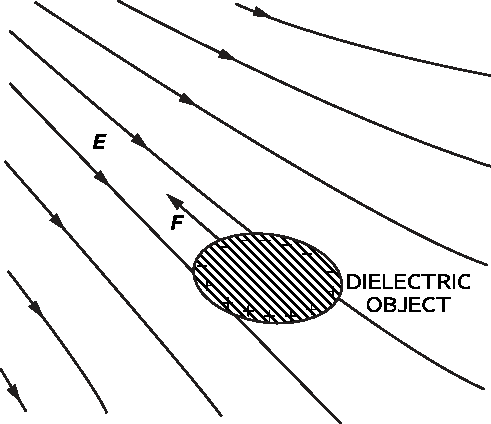
\includegraphics[width=0.8\linewidth]{fyz_fig0712.pdf}
      \caption{V nehomogenním poli působí na dielektrické těleso síla směřující do prostoru s vyšší
              intenzitou pole. (\cite[s.~184]{Feynman02})}
      \label{fyz:fig0712}
    \end{figure}

    Můžeme to vysvětlit polarizací dielektrika, nacházejícího se v elektrickém poli. Vznikají
    polarizační náboje obou znamének, které jsou hřebenem přitahovány, resp. odpuzovány. Výsledkem
    však bude přitahování, protože blíže k hřebenu je pole silnější než dál od něj - hřeben není
    nekonečnou rovinou. Jeho náboj je lokalizovaný. Neutrální kousíček papíru se nepřitáhne ani k
    jedné z elektrod rovinného kondenzátoru. Nehomogenita pole představuje podstatnou část
    mechanizmu přitahování.

    Jak ukazuje obr. \ref{fyz:fig0712}, je dielektrikum vždy přitahováno z oblasti se slabým polem do
    oblasti se silnějším polem. Je možné dokázat, že pro malá tělesa je síla přímo úměrná gradientu
    druhé mocniny intenzity elektrického pole. Proč závisí na druhé mocnině intenzity pole? Protože
    indukované polarizační náboje jsou přímo úměrné polím a pro dané náboje jsou síly přímo úměrné
    poli. Ale jak jsme právě naznačili, bude výsledná síla nenulová pouze tehdy, když se druhá
    mocnina pole od bodu k bodu mění. Součinitel úměrnosti obsahuje mezi jiným permitivitu tělesa a
    závisí i na velikosti a tvaru tělesa.

    \begin{figure}[ht!] %\ref{fyz:fig0713}
      \centering
      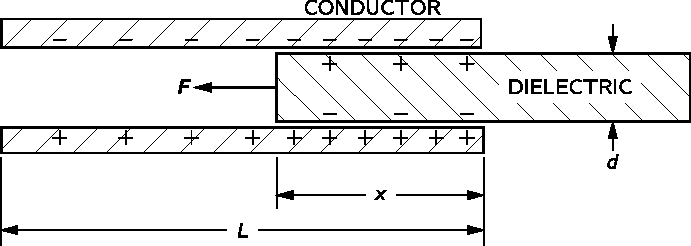
\includegraphics[width=0.9\linewidth]{fyz_fig0713.pdf}
      \caption{Sílu působící v deskovém kondenzátoru na dielektrickou destičku můžeme vypočítat
               použitím principu zachování energie. (\cite[s.~707]{Feynman02})}
      \label{fyz:fig0713}
    \end{figure}

    Existuje příbuzná úloha, v níž je možné vypočítat sílu působící na dielektrikum zcela přesně.
    Máme-li deskový kondenzátor s dielektrickou destičkou vsunutou mezi elektrody pouze částečně
    {obr. \ref{fyz:fig0713}), vznikne síla vtahující dielektrikum dovnitř. Podrobné prozkoumání této
    síly je velmi složité; souvisí s nehomogenitami pole v blízkosti hran dielektrika a elektrod.
    Ale odhlédneme-li od téchto detailů a použijeme pouze princip zachování energie, můžeme sílu
    jednoduše vypočítat. Najdeme ji ze vzorce, který jsme už odvodili dříve. Vztah (\ref{fyz:eq934})
    je ekvivalentní se vztahem
    \begin{equation}\label{fyz:eq937}
      F_x=-\diffp{U}{x}=-\frac{Q^2}{2}\diffp{}{x}\left(\frac{1}{C}\right).
    \end{equation}
    Potřebujeme pouze zjistit, jak se kapacita méní v závislosti na poloze dielektrické destičky.

    Předpokládejme, že celková délka elektrod je \(L\), jejich šířka je \(w\), jejich vzájemná
    vzdálenost, jakož i tloušťka dielektrika je \(d\) a vzdálenost, do které bylo dielektrikum
    zasunuto, je \(x\). Kapacita představuje poměr celkového volného náboje na elektrodách k napětí
    mezi nimi. Viděli jsme, že pro dané napětí \(U\) je plošná hustota volného náboje
    \(\varepsilon_r\varepsilon_0U/d\). Celkový náboj na elektrodách tedy je
    \begin{equation*}
      Q=\frac{\varepsilon_r\varepsilon_OU}{d}xW+\dfrac{\varepsilon_O U}{d}(L-x)W,
    \end{equation*}

  \section{Příklady a cvičení}\label{fyz:IIchapXsecVI}



\todo[inline]{Kapitola fey2ch10 je nedodělaná, obsahuje pouze obrázky}
%} %tikzset
%---------------------------------------------------------------------------------------------------

  % % !TeX spellcheck = cs_CZ
%---------------------------------------------------------------------------------------------------
% file fey2ch42.tex
%---------------------------------------------------------------------------------------------------
%=========================== Kapitola: Zakřivený prostor ===========================================
\setchaptertoc
\chapter{Zakřivený prostor}\label{fyz:IIchapXLII}
  \section{Zakřivené prostory se dvěma rozměry}\label{fyz:IIchapXLIIsecI}
    Podle Newtona se vše navzájem přitahuje silou, která je nepřímo úměrná druhé mocnině vzájemné 
    vzdálenosti, a tělesa reagují na síly zrychleními, která jsou silám úměrná. To jsou Newtonovy 
    zákony obecného gravitačního působení a pohybu. Jak víte, vysvětlují pohyby míčů, planet, 
    oběžnic, galaxií atd.
    
    Einstein vytvořil jinou interpretaci zákona gravitace. Podle ní prostor a čas, které dohromady 
    tvoří \textbf{časoprostor}, jsou v blízkosti velkých hmotností \emph{zakřiveny}. Pohyb těles, 
    jak jej známe, je důsledkem jejich snahy pohybovat se po „přímkách“ v zakřiveném prostoru. Je 
    to velmi, velmi, rafinovaná myšlenka, kterou chceme v této kapitole objasnit.
    
    Naše téma se skládá ze tří částí. Jedna se zabývá gravitačními jevy. Druhá obsahuje myšlenku 
    časoprostoru, kterou jsme se už zabývali. Třetí zahrnuje pojem \emph{zakřiveného časoprostoru}. 
    Na začátku všechno zjednodušíme tím, že se nebudeme starat o gravitaci a vynecháme čas-budeme 
    hovořit jen o zakřiveném prostoru. Později si všimneme i ostatních složek, ale nyní se 
    soustředíme na myšlenku zakřiveného prostoru: co se rozumí zakřiveným prostorem, nebo přesněji, 
    co se pod ním rozumí v této konkrétní Einsteinově aplikaci. I toto je obtížné v případě 
    trojrozměrného prostoru. Proto nejdříve problém ještě více zredukujeme a promluvíme si o tom, 
    co se rozumí pojmem „zakřivený prostor“ ve dvou rozměrech.

    \begin{figure}[ht!] %\ref{fyz:fig516}
      \centering
      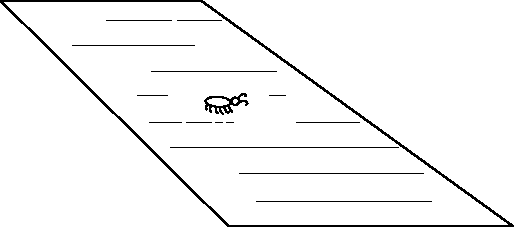
\includegraphics[width=0.7\linewidth]{fyz_fig516.pdf}
      \caption{Brouk na rovině (\cite[s.~775]{Feynman02})}
      \label{fyz:fig516}
    \end{figure}
    
    Abychom pochopili myšlenku zakřiveného prostoru ve dvou rozměrech, musíme si uvědomit omezené 
    pozorovací schopnosti obyvatele takového prostoru. Představme si brouka bez očí, který žije na 
    rovině, jak ukazuje obr. \ref{fyz:fig516}. Může se pohybovat jen po rovině a nemá možnost 
    zjistit, že lze objevit nějaký „vnější svět“. (Nemá naši představivost.) Samozřejmě, naše úvahy 
    se budou zakládat na analogii. My žijeme v trojrozměrném světě a nemáme představu, jak z něj 
    lze vyjít nějakým novým směrem; musíme si tedy pomoci analogií. Je to tak, jako bychom byli 
    brouky na rovině, ale v jiném směru by existoval prostor. Proto se nejdříve budeme zabývat 
    broukem a budeme předpokládat, že musí žít na své ploše a nemůže ji opustit.
    
    Jako jiný příklad brouka, žijícího ve dvou rozměrech, si představte takového, který žije na 
    povrchu koule. Představujeme si, že se může procházet po povrchu koule jako na obr. 
    \ref{fyz:fig517}, ale nemůže se podívat „nahoru“, ani „dolů“, ani „ven“.
    
    \begin{figure}[ht!] %\ref{fyz:fig517}
      \centering
      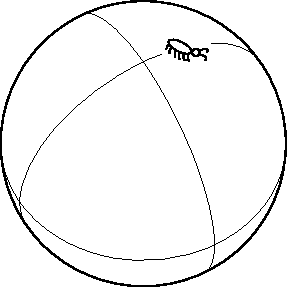
\includegraphics[width=0.5\linewidth]{fyz_fig517.pdf}
      \caption{Brouk na kouli (\cite[s.~775]{Feynman02})}
      \label{fyz:fig517}
    \end{figure}
    
    Dále si všimneme třetí bytosti.Je to opět brouk jako oba předcházející a žije na rovině jako 
    náš první brouk, ale rovina je tentokrát zvláštní. Její teplota je na různých místech různá. 
    Navíc brouk i všechna jeho pravítka jsou z látky, která se roztahuje, je-li zahřáta. Kdykoliv 
    položí své pravítko na nějaké místo, aby si něco změřil, pravítko se okamžitě roztáhne na 
    délku, která přísluší teplotě v daném místě. Kdykoliv položí nějaké těleso, sebe, pravítko, 
    trojúhelník, cokoliv, těleso se v důsledku teplotní roztažnosti zvětší. Vše je na horkých 
    místech delší než na chladných a vše má stejný koeficient teplotní roztažnosti. Domov tohoto 
    třetího brouka budeme nazývat \uv{zahřátá plotýnka} ačkoliv budeme mít na mysli speciální druh 
    takové plotýnky, která je chladná ve středu a zahřívá se směrem k okrajům (obr. 
    \ref{fyz:fig518}).
    
    \begin{figure}[ht!] %\ref{fyz:fig518}
      \centering
      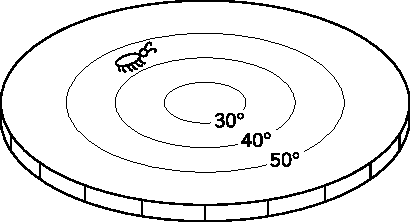
\includegraphics[width=0.7\linewidth]{fyz_fig518.pdf}
      \caption{Brouk na ohřáté desce (\cite[s.~776]{Feynman02})}
      \label{fyz:fig518}
    \end{figure}
    
    Nyní si představíme, že naši brouci začnou studovat geometrii. Ačkoliv si představujeme, že 
    jsou slepí, takže nevidí „vnější“ svět, dokáží pomocí tykadel a nohou mnoho věcí. Umí kreslit 
    čáry, vyrábět pravítka a měřit délky. Začnou od nejjednoduššího geometrického pojmu. Naučí se 
    nakreslit úsečku - nejkratší spojnici dvou bodů. Náš první brouk (viz obr. \ref{fyz:fig519}) se 
    naučí kreslit velmi pěkné čáry. Co se však stane našemu broukovi na kouli? Nakreslí svou úsečku 
    jako nejkratší - pro něj nejkratší - spojnici dvou bodů (obr. \ref{fyz:fig520}). Nám může 
    připadat jako křivka, on  se však od koule vzdálit nemůže, aby zjistil, že „ve skutečnosti“ 
    existuje i kratší úsečka. On jen ví, že vyzkouší-li ve svém světě jinou cestu, je každá delší 
    než jeho úsečka. Jeho úsečkou je tedy nejkratší oblouk mezi dvěma body. (Je to, samozřejmě, 
    oblouk tzv. hlavní kružnice.)

    \begin{figure}[ht!] %\ref{fyz:fig519}
      \centering  
      \subcaptionbox{\label{fyz:fig519a}}{\luafigure[0.5]{fyz_fig519a.pdf}}    \newline
      \subcaptionbox{\label{fyz:fig519b}}{\luafigure[0.5]{fyz_fig519b.pdf}}                 
      \caption{\uv{Úsečka} v rovině a na kouli (\cite[s.~776]{Feynman02})}
      \label{fyz:fig519}
    \end{figure}  
    
    Konečně náš třetí brouk z obr. \ref{fyz:fig518} také bude kreslit „úsečky“, které nám budou 
    připadat jako křivky. Například nejkratší vzdálenost mezi \(A\) a \(B\) na obr. 
    \ref{fyz:fig521} bude podobný znázorněné křivce. Proč? Protože když se jeho křivka zakřivuje 
    směrem k teplejším částem jeho ohřáté desky, pravítka se prodlouží (z našeho vševědoucího 
    hlediska) a stačí přiložit pravítko méně krát, abychom dosáhli z \(A\) do \(B\). Pro něj je 
    čára přímá; nemá možnost vědět, že může existovat kdosi v podivném trojrozměrném světě, kdo by 
    za přímku považoval jinou čáru.
    
    \begin{figure}[ht!] %\ref{fyz:fig521}
      \centering
      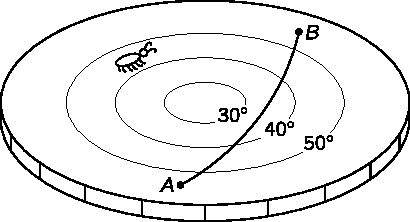
\includegraphics[width=0.7\linewidth]{fyz_fig521.pdf}
      \caption{\uv{Úsečka} na ohřáté desce (\cite[s.~776]{Feynman02})}
      \label{fyz:fig521}
    \end{figure}
    
    Myslím, že jsme pochopili, že celý náš další výklad musí vycházet z hlediska bytostí na různých 
    površích, a ne z našeho hlediska. S tímto vědomím se podíváme, jak bude vypadat zbytek jejich 
    geometrie. Předpokládejme, že všichni brouci se naučili jak nakreslit dvě přímky, které se 
    protínají pod pravým úhlem. (Můžeme zkusit vymyslet, jak by to mohli udělat.) Náš první brouk 
    (ten, co se nachází na obyčejné rovině) zjistí zajímavou věc. Vyjde-li z bodu \(A\), nakreslí 
    úsečku dlouhou \SI{100}{\cm}, pak se otočí o pravý úhel, vyznačí dalších \SI{100}{\cm}, znovu 
    se otočí o \SI{90}{\degree} a projde dalších \SI{100}{\cm}, potřetí udělá pravý úhel a nakreslí 
    čtvrtou stocentimetrovou úsečku, vrátí se do počátečního bodu, jak to znázorňuje obr. 
    \ref{fyz:fig522a}. To je vlastnost jeho světa, jedna ze skutečností jeho „geometrie".
    
    \begin{figure}[ht!] %\ref{fyz:fig522}
      \centering  
      \subcaptionbox{\label{fyz:fig522a}}{\luafigure[0.60]{fyz_fig522a.pdf}}    \newline
      \subcaptionbox{\label{fyz:fig522b}}{\luafigure[0.60]{fyz_fig522b.pdf}}    \newline
      \subcaptionbox{\label{fyz:fig522c}}{\luafigure[0.60]{fyz_fig522c.pdf}}              
      \caption{Čtverec, trojúhelník a kružnice v plochém prostoru (\cite[s.~777]{Feynman02}).}
      \label{fyz:fig522}
    \end{figure}     
    
    Pak objeví jinou zajímavost. Nakreslí-li trojúhelník - obrázek ze tří úseček - součet úhlů je 
    roven \SI{180}{\degree}, tj. součtu dvou pravých úhlů (obr. \ref{fyz:fig522b}).
    
    Dále objeví kružnici. Co je kružnice? Kružnici vytvoříme takto: Vyjdeme po přímkách z jediného 
    bodu mnoha směry a zakreslíte množství bodů, které mají stejnou vzdálenost od daného bodu (obr. 
    \ref{fyz:fig522c}). (Musíme geometrické pojmy pečlivě definovat, abychom dokázali udělat jejich 
    analogii v případě broukových kamarádů.) Samozřejmě, je to ekvivalentní křivce, kterou získáme 
    otočením pravítka kolem bodu. V každém případě se náš brouk naučí nakreslit kružnici. Jednoho 
    dne si pak usmyslí změřit její délku. Změří různé kružnice a zjistí pěknou zákonitost: Délka 
    kružnice je vždy součinem stejného čísla a poloměru \(r\) (což je, samozřejmě, vzdálenost od 
    středu křivky). Obvod a poloměr mají vždy stejný poměr, přibližně \num{6.283}, který nezávisí 
    na velikosti kružnice.

    \begin{figure}[ht!] %\ref{fyz:fig523}
      \centering
      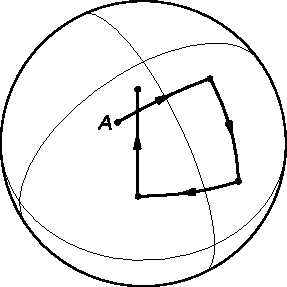
\includegraphics[width=0.5\linewidth]{fyz_fig523.pdf}
      \caption{Pokus nakreslit \uv{čtverec} na kouli
               (\cite[s.~777]{Feynman02})}
      \label{fyz:fig523}
    \end{figure}

    Nyní se podívejme, co objevili ostatní brouci v jejich geometriích. Nejdříve: co se stane, 
    pokusí-li se brouk na kouli nakreslit „čtverec“? Postupuje-li podle popsaných instrukcí, 
    zjistí, že výsledek pravděpodobně nestál za námahu. Dostane křivku jako na obr. 
    \ref{fyz:fig523}. Koncový bod \(B\) nesouhlasí s počátečním bodem \(A\). Vůbec se mu nepodaří 
    získat uzavřený obrazec. Vezměme kouli a vyzkoušejme si to. Podobná věc se přihodí i našemu 
    příteli na ohřáté desce. Zakreslí-li čtyři úsečky stejné délky (změřené pomocí jeho roztažných 
    pravítek), které svírají pravé úhly, získá obrázek znázorněný na obr. \ref{fyz:fig524}.

    \begin{figure}[ht!] %\ref{fyz:fig524}
      \centering
      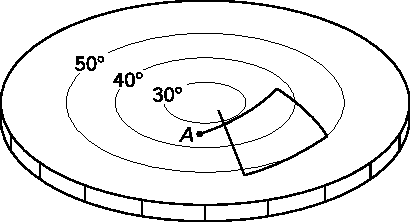
\includegraphics[width=0.7\linewidth]{fyz_fig524.pdf}
      \caption{Pokus nakreslit „čtverec“ na ohřáté desce(\cite[s.~778]{Feynman02})}
      \label{fyz:fig524}
    \end{figure}
   
    Nyní předpokládejme, že naši brouci kdysi měli své Euklidy, kteří jim řekli, jaká by „měla 
    geometrie být“, a že oni si předpovědi ověřili pomocí nepřesných měření v malém měřítku. Když 
    se pak pokusili nakreslit přesné čtverce ve velkém měřítku, zjistili, že něco není v pořádku. 
    Důležité je, že pouze na základě geometrických měření by zjistili, že je na jejich prostoru 
    něco zvláštního. Zakřivený prostor definujeme jako prostor, v němž se geometrie liší od 
    očekávání v rovině. Geometrie brouků na kouli a na ohřáté desce je geometrií v zakřiveném 
    prostoru. Zákony euklidovské geometrie tu selhávají. A vůbec není třeba se vzdálit z roviny, 
    abychom zjistili, zda svět, v němž žijeme je zakřiven. Není třeba obeplouvat zeměkouli, abychom 
    zjistili, že je kulatá. Můžeme zjistit, že žijeme na kouli, tak, že se pokusíme nakreslit 
    čtverec. Je-li čtverec velmi malý, musíme pracovat extrémně přesně, ale je-li čtverec velký, 
    měření lze udělat hrubší.

    \begin{figure}[ht!] %\ref{fyz:fig525}
      \centering
      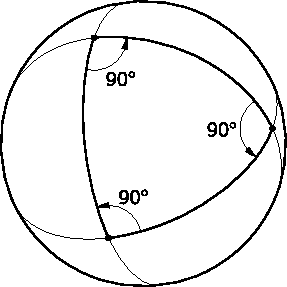
\includegraphics[width=0.7\linewidth]{fyz_fig525.pdf}
      \caption{„Trojúhelník“ na kouli může mít tři pravé úhly (\cite[s.~778]{Feynman02})}
      \label{fyz:fig525}
    \end{figure}
    
    Vezměme si případ trojúhelníka v rovině. Součet jeho úhlů je \num{180} stupňů. Náš přítel na 
    kouli může najít velmi zvláštní trojúhelníky. Může například najít trojúhelníky, které mají tři 
    pravé úhly. Opravdu! Jeden je znázorněn na ob. \ref{fyz:fig525}. Nechť náš brouk vyjde ze 
    severního pólu a nakreslí úsečku až po rovník. Potom se otočí o pravý úhel a projde další 
    úsečku stejné délky. Potom totéž provede znovu. V případě speciální délky, kterou si vybral, se 
    vrátí přesně do počátečního bodu a s první úsečkou se setká pod pravým úhlem. Je tedy 
    nepochybné, že jeho trojúhelník má tři pravé úhly, jejichž součet je \num{270} stupňů. Ukazuje 
    se, že v jeho případě je součet úhlů trojúhelníku vždy větší než \num{180} stupňů. O kolik je 
    větší (v našem speciálním případě o \SI{90}{\degree}), ve skutečnosti závisí na ploše 
    trojúhelníka. Je-li trojúhelník na kouli malý, jeho úhly se sčítají na hodnotu velmi blízkou 
    \num{180} stupňům, jen o maličko větší.
    
    \begin{figure}[ht!] %\ref{fyz:fig526}
      \centering
      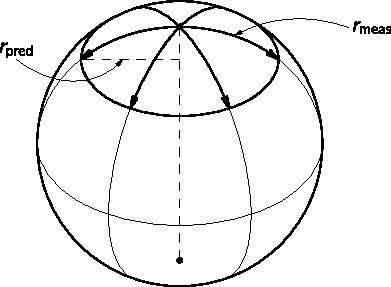
\includegraphics[width=0.7\linewidth]{fyz_fig526.pdf}
      \caption{Kružnice na kouli (\cite[s.~779]{Feynman02})}
      \label{fyz:fig526}
    \end{figure}
     
    Když se trojúhelník zvětšuje, roste i odchylka. Brouci na ohřáté desce by se svými trojúhelníky 
    měli podobné problémy.
    
    Dále se podíváme, co naši brouci zjistí o kružnici. Nakreslí kružnice a změří jejich obvody, 
    Například brouk na kouli by mohl nakreslit kružnici jako na obr. \ref{fyz:fig526}. Přitom by 
    zjistili, že obvod je menší než \(2\pi\)-násobek poloměru. (Díky moudrosti našeho 
    trojrozměrného pohledu vidíme, že to co se nazývá poloměrem, je ve skutečnosti křivka, která je 
    delší než skutečný poloměr kružnice.) Nechť má brouk na kouli prostudovanou euklidovskou 
    geometrii a rozhodne se předpovědět poloměr kružnice tak, že vydělí obvod \(C\) číslem \(2\pi\),
    \begin{equation}\label{fyz:eq528}
      r_{\text{přep}} = \dfrac{C}{2\pi}
    \end{equation}
    
    Pak zjistí, že naměřený poloměr je větší než předpovězený. Aby se s tím nějak vyrovnal, může 
    rozdíl definovat jako „nadbytečný poloměr"
    \begin{equation}\label{fyz:eq529}
      r_{\text{naměř}} - r_{\text{přep}} = r_{\text{nadb}}
    \end{equation}
    a zkoumat, jak nadbytečný poloměr závisí na velikosti kružnice. 
    
    \begin{figure}[ht!] %\ref{fyz:fig527}
      \centering
      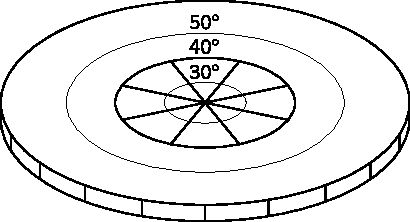
\includegraphics[width=0.7\linewidth]{fyz_fig527.pdf}
      \caption{Kružnice na ohřáté desce
               (\cite[s.~779]{Feynman02})}
      \label{fyz:fig527}
    \end{figure}
    
    Náš brouk na ohřátě desce by objevil podobný jev. Nechť má nakreslit kružnici se středem v 
    chladném bodě desky (obr. \ref{fyz:fig527}). Kdybychom sledovali, jako kreslí kružnici, 
    zjistili bychom, že jeho pravítka jsou blízko středu kratší a prodlužují se směrem od středu, 
    ačkoliv to brouk neví. Když pak měří obvod, jeho pravítko je po celou dobu dlouhé, takže také 
    zjistí, že změřený poloměr je větší než předpovězený, \(C/2\pi\). Brouk na ohřáté desce také 
    objeví „efekt nadbytečného poloměru“. A znovu velikost efektu závisí na poloměru kružnice.
    
    Zakřivený prostor budeme \emph{definovat} jako prostor, v němž se vyskytují tyto typy 
    geometrických chyb: Součet úhlů trojúhelníka se liší od \num{180} stupňů; obvod kružnice dělený 
    číslem \(2\pi\) není roven poloměru; návod na nakreslení čtverce nevede k uzavřenému obrazci. 
    Můžete si vymyslet i jiné.
    
    Uvedli jsme dva různé příklady zakřiveného prostoru: povrch koule a ohřátou desku. Je však 
    zajímavé, že zvolíme-li vhodně způsob, jak se na ohřáté desce mění teplota v závislosti na 
    vzdálenosti, budou obě geometrie úplně stejné. Je to zábavné. Můžeme dosáhnout toho, aby brouk 
    na ohřáté desce dostával přesně stejné výsledky jako brouk na kouli. Předpokládáme-li, že délka 
    pravítek (jako funkce teploty) je úměrná jedné plus konstanta krát druhá mocnina vzdálenosti od 
    počátku, zjistíte, že geometrie ohřáté desky je ve všech podrobnostech přesně stejná jako 
    geometrie koule\footnote{S výjimkou bodu v nekonečnu.}. 
    
    Samozřejmě existují i jiné geometrie. Mohli bychom se zeptat, jaká je geometrie brouka, který 
    žije na hrušce, tj. na povrchu, který má větší zakřivení na jednom místě a menší na jiném, 
    takže přebytek úhlů v trojúhelníku je větší, když brouk nakreslí malý trojúhelník v jedné části 
    svého světa, než když jej nakreslí v jiné. Jinými slovy, křivost prostoru se může od místa k 
    místu měnit. To je jen zobecnění myšlenky zakřiveného prostoru. Totéž lze imitovat i vhodným 
    rozdělením teploty na ohřáté desce. 
    
    \begin{figure}[ht!] %\ref{fyz:fig528}
      \centering
      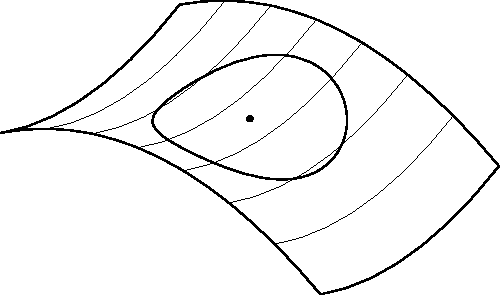
\includegraphics[width=0.7\linewidth]{fyz_fig528.pdf}
      \caption{\uv{Kružnice} na sedlovém povrchu
               (\cite[s.~780]{Feynman02})}
      \label{fyz:fig528}
    \end{figure}
  
    Také je třeba poznamenat, že výsledky by mohly vyjít i s opačným znaménkem. Mohli bychom 
    například zjistit, že všechny trojúhelníky, když jsou velmi velké, mají součet úhlů menší než 
    \num{180} stupňů. Možná že to zní neuvěřitelně, ale není to vůbec tak. Za prvé, mohli bychom 
    mít ohřátou desku, jejíž teplota se vzdáleností od středu klesá. Pak by všechny pozorované 
    efekty měly opačné znaménko. Můžeme toho však dosáhnouti čistě geometricky, podíváme-li se na 
    dvojrozměrnou geometrii sedlového povrchu. Představte si sedlovou plochu jako na obr. 
    \ref{fyz:fig528}. Nakresleme na ní „kružnici“ definovanou jako množinu bodů. které mají od 
    středu stejnou vzdálenost. Tato kružnice je křivka, která po povrchu osciluje a vytváří 
    vroubkovaný okraj. Její obvod je proto větší než očekávaných \(2\pi r\). Takže \(C/2\pi\) je 
    nyní menší než \(r\) a nadbytečný  poloměr je záporný. 
    
    Koule a hrušky apod. jsou všechno plochy s kladnou křivostí; ostatní se nazývají plochy se 
    zápornou křivostí. Obecně dvojrozměrný svět bude mít křivost, která se mění od místa k místu a 
    může být někde kladná a jinde záporná. Pod zakřiveným prostorem obecně chápeme takový prostor, 
    v němž jsou zákony euklidovské geometrie porušeny, ať už je odchylka kladného nebo záporného 
    znaménka. Velikost křivosti (definovaná, řekněme, pomocí nadbytečného poloměru) se může od 
    místa k místu měnit.

    \begin{figure}[ht!] %\ref{fyz:fig529}
      \centering
      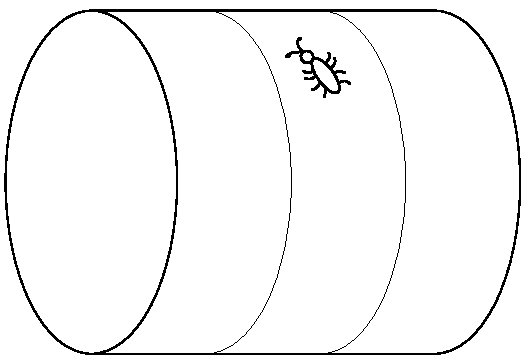
\includegraphics[width=0.7\linewidth]{fyz_fig529.pdf}
      \caption{Dvojrozměrný prostor jehož vnitřní křivost je nulová
               (\cite[s.~781]{Feynman02})}
      \label{fyz:fig529}
    \end{figure}
  
    Ještě poznamenejme, že podle naší definice křivosti není válec kupodivu zakřiven. Kdyby brouk 
    žil na povrchu válce (obr. \ref{fyz:fig527}), zjistil by, že trojúhelníky, čtverce a kruhy, by 
    se chovaly jako v rovině. O tom se lze snadno přesvědčit, představíme-li si, jak by jednotlivé 
    obrazce vypadaly, kdybychom válec rozvinuli do roviny. Pak všechny geometrické obrazce přesně 
    korespondují s tím, co máme v rovině. Pro brouka na válci (předpokládáme, že jej neobejde 
    dokola, ale provádí jen lokální měření) neexistuje způsob, jak zjistit, že je jeho prostor 
    zakřiven. V našem technickém smyslu není jeho prostor zakřiven. Veličina, o níž chceme hovořit, 
    se přesněji nazývá \textbf{vnitřní křivost}, tj. křivost, kterou můžeme objevit na základě 
    měření v lokální oblasti prostoru. (Válec má \emph{nulovou vnitřní křivost}.) Právě v takovém 
    smyslu je třeba chápat Einsteinovo tvrzení, že náš prostor je zakřiven. My jsme však definovali 
    zakřivený prostor pouze ve dvou rozměrech, musíme postoupit dále a podívat se, jaký smysl by 
    tento pojem mohl mít ve třech rozměrech.
    
  \section{Křivost v trojrozměrném prostoru}\label{fyz:IIchapXLIIsecII}
    My žijeme v trojrozměrném prostoru, a proto budeme nyní zvažovat myšlenku, že je náš prostor 
    zakřiven. Můžeme namítnout: „Ale jak si dokážeme představit, že je prostor v nějakém směru 
    zakřiven?“ Pravda, prostor zakřivený v nějakém směru si představit neumíme, neboť naše 
    představivost není dostatečná. (Možná, že je dobře, že si neumíme představit příliš mnoho věcí, 
    takže se alespoň neodtrhneme od reálného světa). Ale křivost můžeme definovat, aniž bychom z 
    našeho trojrozměrného světa vyšli. To, o čem jsme hovořili ve dvou rozměrech, bylo jen 
    rozcvičkou na to, abychom mohli zavést definici křivosti, která nevyžaduje náš „pohled zvenku“.
    
    To, zda náš svět zakřiven je nebo není, můžeme určit způsobem, který je analogický tomu, co 
    používali naši džentlmeni na kouli nebo na ohřáté desce. Možná, že nedokážeme rozlišit dva 
    takové případy, ale jistě můžeme zjistit rozdíl mezi těmito případy a plochým, nezakřiveným 
    prostorem. Dokonce velmi snadno. Nakreslíme trojúhelník a změříme úhly. Nebo vytvoříme velkou 
    kružnici a změříme její obvod a poloměr. Nebo zkusíme vytvořit přesné čtverce, případně 
    krychli. V každém případě zkoumáme, zda platí zákony geometrie. Jestliže neplatí, prohlásíme 
    náš prostor za zakřivený. Nakreslíme-li velký trojúhelník a zjistíme, že součet jeho úhlů 
    překračuje \num{180} stupňů, můžeme říci, že náš prostor je zakřiven. Není-li změřený poloměr 
    kružnice roven jejímu obvodu dělenému číslem \(2\pi\), můžeme prohlásit, že náš prostor je 
    zakřiven.
    
    Jistě si všimneme, že situace ve třech rozměrech může být mnohem složitější než ve dvou. Na 
    libovolném místě ve dvou rozměrech má křivost určitou velikost. Ale ve třech rozměrech může mít 
    křivost několik složek. Nakreslíme-li trojúhelník v nějaké rovině, výsledek může být jiný, než 
    když orientujeme rovinu trojúhelníka jiným způsobem. Nebo vezměme jako příklad kružnici. 
    Představte si, že nakreslíme kružnici, změříme její poloměr a zjistíme, že se neshoduje s 
    \(C/2\pi\), takže tu je nějaký nadbytečný poloměr. Pak nakreslíme jinou kružnici pod pravým 
    úhlem (obr. \ref{fyz:fig530}). Není důvod, proč by nadbytek měl být stejný v případě obou 
    kružnic. Ve skutečnosti v případě kružnice v jedné rovině může být nadbytek kladný a ve druhé 
    rovině záporný (úbytek).
    
    \begin{figure}[ht!] %\ref{fyz:fig530}
      \centering
      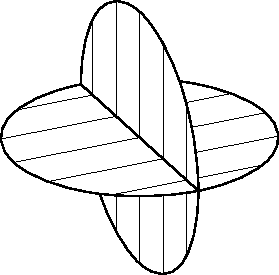
\includegraphics[width=0.5\linewidth]{fyz_fig530.pdf}
      \caption{Nadbytečný poloměr může být různý u kružnic s různými orientacemi      
               (\cite[s.~782]{Feynman02})}
      \label{fyz:fig530}
    \end{figure}
    
    Možná, že přemýšlíme o lepším nápadu: nemůžeme se zbavit všech složek tak, že ve třech 
    rozměrech použijeme kouli? Povrch koule můžeme definovat jako množinu bodů, které jsou od 
    daného bodu v prostoru stejně vzdáleny. Velikost povrchu pak můžeme změřit tak, že na ni 
    položíme jemnou pravoúhlou mřížku a sečteme všechny malé plošky. Podle Euklida má být celková 
    plocha \(S\) rovna \(4\pi\) krát druhá mocnina poloměru; „předpovídaný“ poloměr tedy můžeme 
    definovat jako \(\sqrt{S/4\pi}\). Poloměr však můžeme změřit také přímo tak, že provrtáme díru 
    do středu a změříme jeho vzdálenost. Opět můžeme od změřeného poloměru odečíst předpovídaný 
    poloměr a rozdíl nazvat nadbytkem poloměru:
    \begin{equation*}
      r_{\text{nadb}} = r_{\text{naměř}} -\left(\dfrac{\text{změřený povrch}}{4\pi}\right)^{1/2},
    \end{equation*}
    což by mohlo být dobrou mírou křivosti. Má tu velkou výhodu, že nezávisí na tom, jak 
    zorientujeme trojúhelník nebo kruh.
    
    Ale nadbytečný poloměr koule má i nevýhodu: necharakterizuje prostor úplně. Udává pouze 
    \emph{střední křivost} trojrozměrného světa, protože průměruje přes různé křivosti. Jelikož je 
    to jen průměr, neřeší úplně problém, jaká je geometrie prostoru. Známe-li pouze toto číslo, 
    nemůžeme předpovědět všechny vlastnosti geometrie prostoru, neboť nedokážeme říci co se stane s 
    kružnicemi, které mají různou orientaci. Úplná definice vyžaduje zadání šesti hodnot křivosti v 
    každém bodě. Matematici samozřejmě vědí, jak tato čísla vypočítat. Jednou si v matematické 
    knize můžeme přečíst, jak je všechny zapsat v elegantním a dokonalém tvaru, ale nejdříve je 
    lepší zhruba pochopit, o čem to vlastně budeme psát. Proto, co je naším cílem v naší kapitole, 
    většinou vystačíme se střední křivostí\footnote{Pro úplnost je třeba zmínit ještě jednu 
    okolnost. Jestliže chceme přenést model zakřiveného prostoru jako ohřátou desku do tří rozměrů, 
    musíme si představit, že délka pravítka závisí nejen na místě, ale i na orientaci, kterou má 
    když jej přiložíme. Je to zobecnění jednoduchého případu, kdy délka pravítka závisí jen na 
    místě, ale je stejná jestliže má směr ze severu na jih, z východu na západ, nebo shora dolů. 
    Toto zobecnění je nevyhnutelné, chceme-li pomocí tohoto modelu reprezentovat trojrozměrný 
    prostor s libovolnou geometrií, ačkoliv to shodou okolností nebylo třeba ve dvou rozměrech.}.

  \section{Náš prostor je zakřiven}\label{fyz:IIchapXLIIsecIII}
    Nyní přichází na řadu nejdůležitější otázka. Je pravda, že náš fyzikální trojrozměrný svět, v 
    němž žijeme je opravdu zakřiven? Od okamžiku, kdy mají lidé dost představivosti, aby si 
    uvědomili, že prostor může být zakřiven, je lidský duch zvědavý, zda je skutečný svět zakřiven 
    nebo ne. Mnozí uskutečnili přímá geometrická měření, ale nezjistili žádné odchylky. Na druhou 
    stranu, na základě úvah o gravitaci objevil Einstein, že prostor je \emph{opravdu} zakřiven. 
    Řekneme si, jaký je Einsteinův zákon pro hodnotu křivosti, a také něco o tom, jak k němu dospěl.
    
    Einstein zjistil, že prostor je zakřiven a hmota je zdrojem křivosti. (Hmota je také zdrojem 
    gravitace, takže gravitace souvisí s křivostí, ale k tomu se ještě v této kapitole vrátíme.) 
    Předpokládejme, abychom si problém zjednodušili, že hmota je spojitě rozložena s určitou 
    hustotou, která se však podle potřeby může od místa k místu měnit\footnote{Nikdo (dokonce ani 
    Einstein) neví, jak postupovat, je-li hmota soustředěna do bodů}. Einsteinovo pravidlo pro 
    výpočet křivosti je následující. Máme-li oblast prostoru, v níž se nachází hmota, a v ní 
    vybereme dostatečně malou kouli, takže hustota hmoty \(\varrho\) v ní je v podstatě konstantní, 
    je \emph{nadbytečný poloměr} koule úměrný množství hmoty v kouli. Podle definice nadbytečného 
    poloměru platí
    \begin{equation}\label{fyz:eq530}
      \text{nadbytečný poloměr } = \sqrt{\dfrac{S}{4\pi}} - r_\text{naměř} 
                                 = \dfrac{\varkappa}{3c^2}\cdot M.
    \end{equation}
    kde \(\varkappa\) je \emph{Newtonova gravitační konstanta}, \(c\) je \emph{rychlost světla} a 
    \(M=4\pi\varrho r^3/3\) je hmotnost látky uvnitř koule. To je Einsteinův vztah pro 
    \textbf{střední křivost prostoru}. 
    
    Vezměme si jako příklad naší Zemi a zapomeňme, že její hustota se od bodu k bodu mění, abychom 
    nemuseli počítat žádné integrály. Předpokládejme, že bychom její povrch změřili velmi pečlivě, 
    a pak vykopali díru do středu a změřili její poloměr. Z velikosti povrchu bychom mohli 
    vypočítat předpovídaný poloměr tak, že bychom povrch brali jako \(4\pi r^2\). Pokud bychom 
    porovnali předpovídaný poloměr se skutečným, zjistili bychom, že skutečný poloměr převyšuje 
    předpovídaný poloměr o hodnotu, kterou udává vztah (\ref{fyz:eq530}). Konstanta 
    \(\varkappa/3c^2\) 
    je rovna asi \SI{2.5e-28}{\m\per\kg}, takže na každý kilogram látky, je odchylka naměřeného 
    poloměru \SI{2.5e-28}{\m}. Dosadíme-li hmotnost Země, která je přibližně \SI{6e24}{\kg} vyjde, 
    že zemský poloměr je asi o \SI{1.5}{\mm} větší, než by měl odpovídat velikosti jejího 
    povrchu\footnote{Přibližně, neboť hustota není nezávislá na poloměru, jak jsme předpokládali.}. 
    Pokud bychom stejný výpočet zopakovali pro Slunce, zjistili bychom, že poloměr Slunce je o půl 
    kilometru větší, než by měl být. 
    
    Všimněme si, že zákon říká, že \emph{střední} křivost nad povrchem země je nulová. To však 
    neznamená že všechny složky křivosti jsou nulové. I nad Zemí může být - a ve skutečnosti je - 
    určité zakřivení. V případě kružnice v rovině bude existovat nadbytečný poloměr jednoho 
    znaménka při jistých orientacích roviny a opačného znaménka při jiných. Pouze průměr přes kouli 
    vychází nulový, když se \emph{uvnitř} nenachází žádná látka. Shodou okolností se ukazuje, že 
    existuje vztah mezi různými složkami křivosti a \emph{změnami} průměrné křivosti od místa k 
    místu. Tudíž známe-li průměrnou křivost v celém prostoru můžete detailně vypočítat křivost v 
    každém bodě. Střední křivost nad zemí se mění s výškou, takže i tam je prostor zakřiven. A 
    právě toto zakřivení se nám jeví jako gravitační síla. 
    
    Představme si brouka na rovině. Nechť na povrchu roviny existují drobné „puchýřky“. Kdykoliv 
    brouk narazí na „puchýřek“ usoudí, že jeho prostor má malou lokální oblast zakřivení. Něco 
    podobného máme ve třech rozměrech. Všude, kde se nacházejí shluky látky, má náš trojrozměrný 
    prostor lokální zakřivení - jakýsi trojrozměrný „puchýřek“. 
    
    Vytvoříme-li na rovině mnoho hrbolů, může být jejich výsledkem vedle všech „puchýřků“ i 
    globální křivost - prostor může vypadat jako koule. Bylo by zajímavé vědět, zda má náš prostor 
    takovou výslednou průměrnou křivost, jakož i lokální „puchýřky“ v důsledku shluků hmoty, jakými 
    jsou například Země a Slunce. Astrofyzikové hledají odpověď na tuto otázku na základě měření 
    galaxií ve velkých vzdálenostech. Například, liší-li se počet galaxií, který vidíme v kulové 
    slupce ve velké vzdálenosti, od našich očekávání na základě velikost poloměru slupky, máme míru 
    nadbytečného poloměru obrovské koule. Existuje naděje, že na základě takovýchto měření můžeme 
    zjistit, je-li náš vesmír jako celek v průměru plochý nebo zakřivený, zda je „uzavřený“ (jako 
    koule) nebo „otevřený“ (jako rovina). Možná, že jsme něco slyšeli o debatách, které se na toto 
    téma vedou. Diskutuje se velmi, neboť astronomická měření jsou stále ještě zcela nekonkluzivní; 
    experimentální údaje nejsou dost přesné, aby poskytly definitivní odpověď. Bohužel, nemáme ani 
    nejmenší představu o tom, jaká je globální křivost našeho Vesmíru.
    
  \section{Geometrie v časoprostoru}\label{fyz:IIchapXLIIsecIV}
    Nyní musíme něco říci o čase. Jak víme ze speciální teorie relativity, měření v prostoru a 
    měření v čase navzájem souvisí. A bylo by trochu bláznivé, kdyby se něco dělo s prostorem, 
    přičemž čas by v tom nehrál určitou úlohu. Pamatujeme si, že měření času závisí na rychlosti, 
    jakou se pohybujeme. Například pozorujeme-li chlapíka, který kolem nás proletí v raketě, 
    vidíme, že u něj vše probíhá pomaleji než u nás. Řekněme, že se vydá na cestu a vrátí se 
    \emph{podle našich hodin} přesně za \num{100} sekund; jeho hodiny mohou ukazovat, že byl pryč 
    jen \num{95} sekund. Ve srovnání s našimi běžely jeho hodiny, jakž i jiné procesy, např. údery 
    srdce, pomaleji.
    
    Všimněme si zajímavého problému. Předpokládejme, že vy jste ten chlapík v raketě. Požádáme vás, 
    abyste vystartovali na daný signál a vrátili se do výchozího místa přesně včas, abyste stihli 
    další signál - řekněme přesně o 100 sekund později podle našich hodin. A také od vás chceme, 
    abyste výlet uskutečnili tak, aby vaše hodiny ukazovaly co nejdelší \emph{uplynulý} čas. Jak se 
    máte pohybovat? Měli byste zůstat stát. Pohnete-li se, vaše hodiny budou ukazovat po návratu 
    méně než \num{100} sekund. 
    
    Ale předpokládejme, že úlohu trochu změníme. Požádáme vás, abyste vyšli z bodu \(A\) na daný 
    signál a dorazili do bodu \(B\) (oba body se vůči vám nepohybují), a to tak, že se vrátíte 
    přesně v okamžiku druhého signálu (řekněme o \num{100} sekund později podle našich nehybných 
    hodin). A opět se po vás chce, abyste výlet uskutečnili tak, že po návratu budou vaše hodinky 
    ukazovat co nejvyšší hodnotu. Jak byste to udělali? Pro jakou trajektorii a jaký jízdní řád 
    budou vaše hodiny ukazovat při příchodu největší uplynulý čas? Odpověď je, že z vašeho hlediska 
    bude výlet nejdelší, uskutečníte-li ho stálou rychlostí po přímce. Důvod je ten, že každý pohyb 
    navíc a každý vzrůst rychlosti zpomalí vaše hodiny. (Jelikož časové rozdíly závisejí na druhé 
    mocnině rychlosti, to, co ztratíte příliš rychlým pohybem na jednom místě, nikdy nedoženete 
    velmi pomalým pohybem na místě jiném.)
     
    Motiv celé této diskuze spočívá v tom, že tento nápad můžeme využít k definici úsečky v 
    časoprostoru. Analogem prostorové úsečky v časoprostoru je \emph{pohyb} konstantní rychlostí v 
    konstantním směru. 
    
    Křivce s nejmenší délkou v prostoru neodpovídá v časoprostoru dráha s nejkratším, ale s 
    \emph{nejdelším} časem, v důsledku zábavných věcí, které se dějí se znaménky časových členů v 
    teorii relativity. Pohyb „po přímce" - analog „konstantní rychlostí na přímce" -je tedy ten 
    pohyb, který přenese hodiny z jednoho místa v jednom čase na jiné místo v jiném čase tak, že 
    údaj na hodinách ukáže nejdelší uplynulý čas. To bude naše definice analogu úsečky v 
    časoprostoru.
    
  \section{Gravitace a princip ekvivalence}\label{fyz:IIchapXLIIsecV}
    Jsme připraveni přejít k zákonům gravitace. Einstein usilovalo vytvoření teorie gravitace, jež 
    by byla ve shodě s teorií relativity, kterou vytvořil dříve. Snažil se marně do té doby, než se 
    zachytil principu, který jej dovedl ke správným zákonům. Tento princip je založen na myšlence, 
    že padá-li nějaký předmět volným pádem, vše se v něm zdá být ve stavu beztíže. Například 
    družice na oběžné dráze padá volně v poli zemské přitažlivosti a proto se v něm astronaut cítí 
    bez tíže. Tato myšlenka, zformulovaná podstatně přesněji, se nazývá \textbf{Einsteinův princip 
    ekvivalence}. Souvisí se skutečností, že všechna tělesa padají se stejným zrychlením bez ohledu 
    na jejich hmotnost a na to, z čeho se skládají. Pohybuje-li se raketa bez motorů, tj. vlastně 
    volným pádem, a v ní se nachází člověk, zákony, které řídí pád člověka i rakety jsou stejné. 
    Přemístí-li se do středu rakety, zůstane tam. \emph{Vzhledem k raketě} nepadá. To máme na 
    mysli, když říkáme, že je v beztížném stavu.
    
    Dále si představte, že jste v raketě, která se pohybuje se zrychlením. Se zrychlením vzhledem k 
    čemu? Řekněme, že její motory jsou zapnuty a vytvářejí tah, takže raketa nepluje volným pádem. 
    Také si představte, že  jste daleko v prázdném prostoru, takže na raketu nepůsobí prakticky 
    žádné gravitační síly. Je-li zrychlení rakety právě \(g\) dokážete stát na její podlaze a 
    cítíte svou normální tíhu. Pustíte-li míč, bude padat na podlahu. Proč? Protože raketa se 
    zrychluje směrem nahoru, ale míč necítí žádné síly, a proto nezrychluje a setrvává. Uvnitř 
    rakety se zdá, že míč má zrychlení \(g\) směrem dolů.
    
    Tuto situaci porovnejme s tím, co se děje v raketě, která klidně odpočívá na povrchu Země. 
    \emph{Vše je stejné!} Přitahuje nás to k Zemi, míč padá se zrychlením \(g\) atd. Skutečně, jak 
    můžete uvnitř rakety usoudit, zda sedíte na Zemi, nebo se zrychlujete ve volném prostoru? Podle 
    Einsteinova principu ekvivalence neexistuje způsob jak rozlišit obě situace, provádíte-li 
    měření toho, co se děje uvnitř rakety!
    
    Abychom byli zcela přesní, platí to jen pro jeden bod uvnitř rakety. Gravitační pole Země není 
    přesně homogenní, takže míč, který padá volným pádem, má na různých místech trochu jiná 
    zrychlení - mění se jejich směr i velikost. Ale představíme-li si absolutně homogenní 
    gravitační pole, bude takové pole dokonalé a v každém ohledu imitováno systémem s konstantním 
    zrychlením. To je základ principu ekvivalence.
    
  \section{Chod hodin v gravitačním poli}\label{fyz:IIchapXLIIsecVI}
    Princip ekvivalence využijeme k výpočtu zajímavého jevu, k němuž dochází v gravitačním poli. 
    Ukážeme si, jaká věc se stává v raketě. Zřejmě bychom něco podobného v gravitačním poli 
    neočekávali. Umístíme jedny hodiny do „hlavy“ rakety, tj. do jejího předního konce, a stejné 
    hodiny do jejího „ocasu“ jako na obr. \ref{fyz:fig531}. Nazvěme tyto hodiny \(A\) a \(B\). 
    Porovnáme-li údaje obou hodin, když raketa zrychluje, zdá se, že přední hodiny jdou rychleji 
    než hodiny zadní. Abychom se o tom přesvědčili, představme si, že přední hodiny vysílají 
    záblesk světla každou sekundu a že my sedíme v ocasu a porovnáváme příchod záblesků světla s 
    tikáním hodin \(B\). Řekněme, že se raketa nachází v poloze \(a\) na obr. \ref{fyz:fig532}, 
    když hodiny \(A\) vyšlou záblesk, a v poloze \(b\), když záblesk dojde k hodinám \(B\). Později 
    bude raketa v poloze \(c\), když hodiny \(A\) vyšlou další záblesk, a v poloze \(d\), když 
    uvidíme jeho příchod k hodinám \(B\).
    

    \begin{figure}[ht!] %\ref{fyz:fig531}
      \centering
      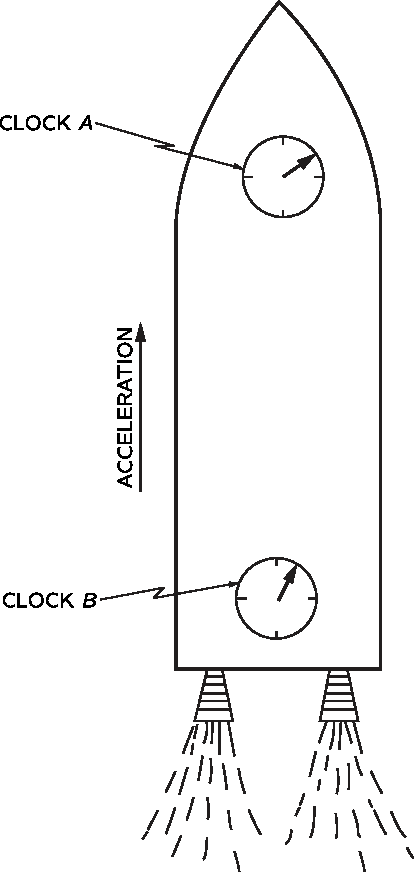
\includegraphics[width=0.5\linewidth]{fyz_fig531.pdf}
      \caption{Zrychlující se raketa se dvěma hodinami (\cite[s.~786]{Feynman02})}
      \label{fyz:fig531}
    \end{figure}
    
    První záblesk projde vzdálenost \(L_1\), zatímco druhý kratší vzdálenost \(L_2\). Vzdálenost je 
    kratší, neboť raketa se zrychluje a v okamžiku druhého záblesku má vyšší rychlost. Vidíme, že 
    pokud byly oba záblesky z hodin \(A\) vyslány s jednosekundovým časovým posunem, dojdou k 
    hodinám \(B\) oddělené intervalem kratším než sekunda, neboť druhý záblesk na cestě stráví 
    kratší dobu.
    
    Totéž se bude dít s pozdějšími záblesky. Kdybychom tedy seděli v ocasu, dospěli bychom k 
    závěru, že hodiny \(A\) běží rychleji než \(B\). Pokud bychom provedli celou věc naopak, 
    nechali hodiny \(B\) vysílat světlo a pozorovali jej u hodin \(A\), zdálo by se vám, že hodiny 
    \(B\) běží \emph{pomaleji} než \(A\). Vše souhlasí a není na tom nic záhadného.
    
    Nyní si představme, že raketa je v klidu na zemském povrchu. \emph{Děje se totéž}. Sedíme-li s 
    jedněmi hodinami na podlaze a pozorujeme druhé, které leží na vysoké poličce, zdá se, že běží 
    rychleji než hodiny na podlaze! Řekneme: „To není správně. Časy musí být stejné. V případě bez 
    zrychlení není důvod proč by hodiny neměly jít stejně.“ Musí to však tak být, platí-li princip 
    ekvivalence. Einstein trval na tom, že princip je správný a postupoval odvážně vpřed. 
    Prohlásil, že hodiny na různých místech v gravitačním poli musí zdánlivě jít různými 
    rychlostmi. Jdou-li však vždy \emph{zdánlivě} vzhledem k sobě různou rychlostí, pak vzhledem k 
    prvním hodinám druhé opravdu jinou rychlostí jdou.
    
    Teď vidíme, že tu máme s hodinami analogickou situaci jako se zahřátým pravítkem, o kterém jsme 
    mluvili dříve, když jsme si všímali brouka na zahřáté desce. Představovali jsme si, že pravítka 
    i brouci a vůbec vše se měnilo stejným způsobem při změně teploty, takže brouci nikdy nemohli 
    zjistit, že jejich měřicí pomůcky se změnily při pohybu po ohřáté desce. Podobné je to v 
    případě hodin v gravitačním poli. Každé hodiny, které umístíme na vyšší úroveň, běží viditelně 
    rychleji. Tlukot srdce je rychlejší, všechny procesy probíhají rychleji.

    \begin{figure}[ht!] %\ref{fyz:fig532}
      \centering
      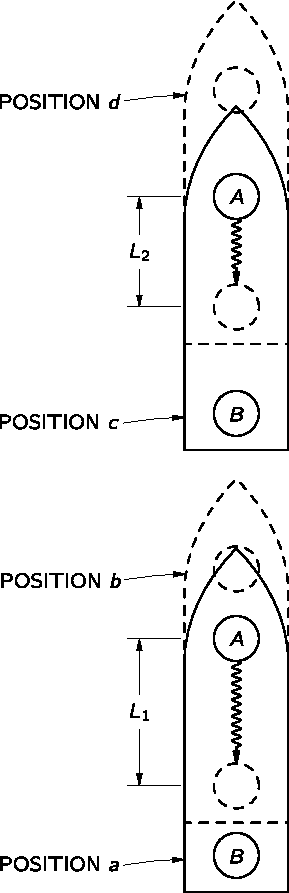
\includegraphics[width=0.5\linewidth]{fyz_fig532.pdf}
      \caption{Hodiny v přední části zrychlující rakety běží zdánlivě rychleji než hodiny v zadní 
               části. (\cite[s.~787]{Feynman02})}
      \label{fyz:fig532}
    \end{figure}
    
    Pokud by to tak nebylo, mohli bychom odlišit gravitační pole od zrychlující vztažné soustavy. 
    Představa, že čas se může od místa k místu měnit, není jednoduchá, ale právě tuto představu 
    Einstein použil, a - věřte nebo nevěřte - je správná.
    
    Pomocí principu ekvivalence můžeme vypočítat, jak se mění rychlost hodin v gravitačním poli s 
    výškou. Stačí vypočítat zdánlivou odchylku mezi dvěma hodinami ve zrychlující se raketě. 
    Nejsnáze to můžeme provést pomocí výsledku pro Dopplerův jev, který jsme odvodili v kapitole 
    \ref{fyz:IchapXXXIV} dílu \ref{part:FYZI}. Tam jsme zjistili (viz vztah (\ref{fyz:eq531})), že 
    je-li \(v\) \emph{relativní} rychlost zdroje a přijímače, souvisí \emph{zachycená} frekvence 
    \(\omega\) s \emph{vyslanou} frekvencí \(\omega_0\) podle vztahu
    \begin{equation}\label{fyz:eq532}
      \omega = \omega_0\dfrac{1+\dfrac{v}{c}}{\sqrt{1-\dfrac{v^2}{c^2}}}.
    \end{equation}
    Zamyslíme-li se nyní nad zrychlující se raketou na obr. \ref{fyz:fig532}, vidíme, že vysílač i 
    přijímač se pohybují v každém okamžiku stejnými rychlostmi. Ale za čas, za který projde 
    světelný signál od hodin \(A\) k \(B\), se raketa zrychlila. Ve skutečnosti nabyla dodatečnou 
    rychlost \(gt\), přičemž \(g\) je zrychlení a \(t\) je čas, za který světlo urazí vzdálenost 
    \(H\) z \(A\) do \(B\). Tento čas je velmi blízký \(H/c\). 
    
    Dojde-li tedy signál k \(B\), zvýšila raketa svou rychlost o \(gH/c\). Přijímač má takovou 
    rychlost vždy vůči rychlosti vysílače v okamžiku, kdy ho signál opustil. To je tedy rychlost, 
    kterou musíme dosadit do vztahu (\ref{fyz:eq532}) pro Dopplerův posun. Předpokládáme-li, že 
    zrychlení a délka kosmické lodi jsou dostatečně malé, takže tato rychlost je mnohem menší než 
    \(c\), můžeme zanedbat členy řádu \(v^2/c^2\). Vyjde nám
    \begin{equation}\label{fyz:eq533}
      \omega = \omega_0\left(1 + \dfrac{gH}{c^2}\right).
    \end{equation}
    
    V případě dvou hodin v raketě platí vztah
    \begin{equation*}
      \binom{\text{frekvence hodin}}{\text{příjímače}} 
        = \binom{\text{frekvence hodin}}{\text{vysílače}}\cdot\left(1 + \dfrac{gH}{c^2}\right)
    \end{equation*}
    přičemž \(H\) je výška vysílače nad přijímačem. 
    
    \emph{Na základě principu ekvivalence musí platit stejný vztah v případě dvojích hodin 
    oddělených výškovým rozdílem \(H\) v gravitačním poli se zrychlením volného pádu} \(g\). 
    
    To je natolik důležitá myšlenka, že bychom vám chtěli dokázat, že vyplývá i z jiného zákona 
    fyziky - ze zákona zachování energie. Víme, že gravitační síla, která působí na těleso, je 
    úměrná její hmotnosti \(M\), která je ve vztahu k celkové vnitřní energii \(E\). \(M=E/c^2\). 
    Například hmotnosti jader určené z energií jaderných reakcí, při nichž dochází k přeměně jader, 
    souhlasí s hmotnostmi získanými z \emph{atomových hmotností}.
    
    Nyní si představme atom, jehož nejnižší energetický stav má celkovou energii \(E_0\) a vyšší 
    stav energii \(E_1\) a který může přejít ze stavu \(E_1\) do stavu \(E_0\), emitováním světla. 
    Frekvence \(\omega\) tohoto světla bude dána vztahem
    \begin{equation}\label{fyz:eq534}
      \hbar\omega = E_1 - E_0.
    \end{equation}
    
    Nechť je takový atom původně na podlaze a přeneseme jej odtud do výšky \(H\). Musíme přitom 
    vykonat práci, která je potřebná k přesunu hmotnosti \(m_1 = E_1/c^2\) proti směru působení 
    gravitační síly. Vykonaná práce je
    \begin{equation}\label{fyz:eq535}
      \dfrac{E_1}{c^2}gH.
    \end{equation}
    
    Pak necháme atom vyslat foton a přejít do nižšího energetického stavu \(E_0\). Poté atom 
    přeneseme zpět na podlahu. Při návratu je hmotnost \(E_0/c^2\); zpět získáme energii
    \begin{equation}\label{fyz:eq536}
      \dfrac{E_0}{c^2}gH,
    \end{equation}
    takže jsme vykonali celkovou práci
    \begin{equation}\label{fyz:eq537}
      \Delta W = \dfrac{E_1 - E_0}{c^2}gH.
    \end{equation}
    
    Když atom emitoval foton, odevzdal energii \(E_1 - E_0\). Představme si, že se foton náhodou 
    vrátil na podlahu a byl absorbován. Kolik energie by odevzdal? V prvním okamžiku bychom si 
    mohli myslet, že by odevzdal energii \(E_1 - E_0\). To však nemůže být pravda, zachovává-li se 
    energie. Na začátku jsme měli energii \(E_1\) na podlaze. Na konci je energie na úrovni podlahy 
    součtem energie \(E_0\) atomu v nižším stavu a energie \(E_{tot}\) absorbovaného fotonu. Mezi 
    tím jsme však museli dodat dodatečnou energii \(\Delta W\) podle vztahu (\ref{fyz:eq537}). 
    Zachovává-li se energie, musí být energie, s níž skončíme na podlaze, větší než počáteční 
    energie o hodnotu vykonané práce. Musí platit
    \begin{subequations}
      \begin{align}
        E_{fot} + E_0 = E_1 + \Delta W       \label{fyz:eq538a}  \\
        \shortintertext{neboli}
        E_{fot} = E_1 - E_1 + \Delta W.      \label{fyz:eq538b}
      \end{align}
    \end{subequations}

    Musí to být tak, že foton na úroveň podlahy \emph{nedopadne} jen s energií \(E_1 - E_0\) s níž 
    byl vyslán, ale s \emph{o něco větší energií}. Jinak by se nějaká energie ztratila. Dosadíme-li 
    do rovnice (\ref{fyz:eq538b}) \(\Delta W\) z rovnice (\ref{fyz:eq537}), vyjde nám, že foton 
    dopadne na úroveň podlahy s energií
    \begin{equation}\label{fyz:eq539}
      E_{fot} = (E_1-E_0)\left(1 + \dfrac{gH}{c^2}\right).
    \end{equation}
    
    Ale foton s energií \(E_{fot}\) má frekvenci \(\omega = E_{fot}/\hbar\). Označíme-li frekvenci 
    \emph{vyslaného} fotonu \(\omega_0\) (musí být podle (\ref{fyz:eq534}) rovna \((E_1 — 
    E_0)\hbar\)), náš výsledek (\ref{fyz:eq539}) vede opět ke vztahu (\ref{fyz:eq533}) mezi 
    frekvencí fotonu absorbovaného na podlaze a frekvencí s jakou byl vyslán.
    
    Stejný výsledek můžeme získat ještě jinak. Foton s frekvencí \(\omega_0\) má energii \(E = 
    \hbar\omega_0\). Jelikož energii \(E_0\) odpovídá gravitační hmotnost \(E_0/c^2\), má foton 
    hmotnost (ne klidovou hmotnost!) \(\hbar\omega_0/c^2\) a je „přitahován“ k Zemi. Při pádu z 
    výšky \(H\) získá  dodatečnou energii \((\hbar\omega_0/c^2)gH\), takže dopadne s energií
    \begin{equation*}
      E = \hbar\omega_0\left(1 + \dfrac{gH}{c^2}\right).
    \end{equation*}
    Jeho frekvence po pádu je \(E/\hbar\), což opět vede k výsledku (\ref{fyz:eq533}). Naše 
    představy o relativitě, kvantové fyzice a zachování energie navzájem souhlasí pouze tehdy, 
    jsou-li Einsteinovy předpovědi o hodinách v gravitačním poli správné. Změny frekvence, o nichž 
    hovoříme, jsou obvykle velmi malé. Například při rozdílu výšek \num{20} metrů u zemského 
    povrchu je rozdíl frekvencí přibližně jen \num{2e-15}. Právě takovou změnu se však podařilo 
    experimentálně změřit pomocí \textbf{Mössbauerova jevu}. Einstein měl úplnou pravdu.
    
  \section{Křivost časoprostoru}\label{fyz:IIchapXVLIIsecVII}
    Nyní bychom chtěli vše, o čem jsme hovořili, dát do souvislosti s představou o zakřiveném 
    časoprostoru. Už jsme poznamenali, že běží-li čas různými rychlostmi na různých místech, je to 
    analogické se zakřiveným prostorem ohřáté desky. Je to však víc než analogie; znamená to, že 
    časoprostor je opravdu zakřiven. Pokusme se o trochu geometrie v časoprostoru. Na první pohled 
    to může vypadat zvláštně, ale vždyť jsme už mnohokrát kreslili časoprostorové diagramy se 
    vzdálenostmi nanesenými na jednu osu a časem na druhou. Zkusme vytvořit pravoúhelník v 
    časoprostoru. Nejprve nakreslíme graf výšky \(Hv\) závislosti na čase \(t\) jako na obr. 
    \ref{fyz:fig533a}. Abychom vytvořili základnu našeho pravoúhelníku, vezmeme si předmět, který 
    je \emph{v klidu} ve výšce a budeme sledovat jeho světočáru \num{100} sekund. Získáme tak 
    úsečku \(BDv\) části \(b\) obrázku, která je rovnoběžná s osou \(t\). Nyní si vezmeme další 
    předmět, který je v čase \(t = 0\) \num{100} metrů nad prvním. Vyjde z bodu \(A\) na obr. 
    \ref{fyz:fig533c}. Nyní sledujme jeho světočáru po dobu \num{100} sekund, kterou měříme pomocí 
    hodin v bodě \(A\). Předmět projde z bodu \(A\) do \(C\) jak znázorňuje část \(d\) obrázku. 
    Všimněme si však, že v důsledku toho, že hodiny v různých výškách jdou různou rychlostí 
    (předpokládáme přítomnost gravitačního pole), body \(C\) a \(D\) nejsou současné. Pokusíme-li 
    se doplnit pravoúhelník úsečkou do bodu \(C\), který leží \num{100} metrů nad bodem \(D\) ve 
    stejném čase (obr. \ref{fyz:fig533e}) obrazec se neuzavře. Právě toto máme na mysli, když 
    říkáme, že časoprostor je zakřiven.
    
    \begin{figure}[ht!] %\ref{fyz:fig533}
      \centering  
      \subcaptionbox{\label{fyz:fig533a}}{\luafigure[0.70]{fyz_fig533a.pdf}}    \newline
      \subcaptionbox{\label{fyz:fig533b}}{\luafigure[0.70]{fyz_fig533b.pdf}}    \newline
      \subcaptionbox{\label{fyz:fig533c}}{\luafigure[0.70]{fyz_fig533c.pdf}}    \newline
      \subcaptionbox{\label{fyz:fig533d}}{\luafigure[0.70]{fyz_fig533d.pdf}}    \newline
      \subcaptionbox{\label{fyz:fig533e}}{\luafigure[0.70]{fyz_fig533e.pdf}}            
      \caption{Pokus vytvořit pravoúhelník v časoprostoru (\cite[s.~790]{Feynman02}).}
      \label{fyz:fig533}
    \end{figure}     

  \section{Pohyb v zakřiveném časoprostoru}\label{fyz:IIchapXVLIIsecVIII}
    Podívejme se na zajímavou hádanku. Máme dvojici identických hodin, \(A\) a \(B\), které leží na 
    povrchu Země jako na obr. \ref{fyz:fig534}. Zvedneme hodiny \(A\) do nějaké výšky \(H\), chvíli 
    je tam podržíme a opět vrátíme na Zem, právě ve chvíli, kdy druhé hodiny \(B\) ušli o \num{100} 
    sekund. Hodiny \(A\) ukáží řekněme \num{107} sekund, neboť nahoře ve vzduchu běžely rychleji. 
    Tady je naše hádanka: Jak máme pohybovat hodinami \(A\) aby ukazovaly co nejvyšší hodnotu 
    uplynulého času, za předpokladu, že se vrátí, když hodiny \(B\) ukazují \num{100} sekund? 
    Řekneme si: „To je snadné. Jednoduše zvedneme hodiny \(A\) co nejvýše. Tam poběží nejrychleji, 
    tudíž uplyne nejvíce času, než se vrátí.“ To je ale chyba. Na něco jste zapomněli - na cestu 
    vzhůru a dolů máme jen \num{100} sekund. Vyrazíme-li velmi vysoko, musíme se vrátit velmi 
    rychle, abychom prošli tam a zpět za \num{100} sekund. A nesmíme zapomenou na efekt speciální 
    relativity, který způsobuje, že se pohybující hodiny \emph{zpomalí} \(\sqrt{V1 - 
    v2/c^2}\)-krát. Tento relativistický jev způsobuje, že hodiny \(A\) ukazují \emph{menší} čas 
    než hodiny \(B\). Vidíme, že tu máme zajímavou hru.
    
    \begin{figure}[ht!] %\ref{fyz:fig534}
      \centering
      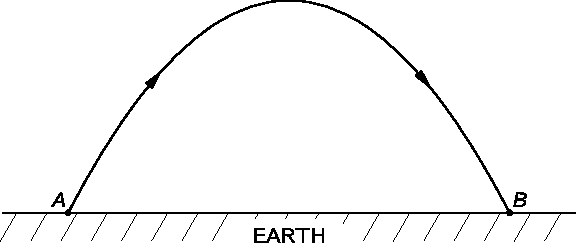
\includegraphics[width=0.9\linewidth]{fyz_fig534.pdf}
      \caption{V homogenním gravitačním poli je trajektorie s maximálním vlastním časem při dané 
               hodnotě uplynulého času parabola
               (\cite[s.~791]{Feynman02})}
      \label{fyz:fig534}
    \end{figure}
    
    Nebudeme-li hodinami \(A\) hýbat, dostaneme \num{100} sekund. Přesuneme-li je do malé výšky a 
    pomalu se vrátíme, získáme o trochu více než \num{100} sekund. Posuneme-li je o kousek výše, 
    získáme možná ještě o trochu víc. Posuneme-li je příliš vysoko, musíme se pohybovat rychle, a 
    tak zpomalit naše hodiny na tolik, že se vrátíme s méně než \num{100} sekundami. Jaký jízdní 
    řád, jaká závislost výšky na čase, nám dá nejvyšší možnou hodnotu na hodinách \(A\)? Jak vysoko 
    se máme posunout, jakou pečlivě vybranou rychlostí se tam máme dostat, abychom se k hodinám 
    \(B\) vrátili právě v okamžiku, kdy na nich uplyne \num{100} sekund?
    
    Odpověď je následující. Vypočítejme, jak rychle musíme vyhodit míč směrem vzhůru do vzduchu, 
    aby na zem dopadl přesně za \num{100} sekund. Pohyb míče – nejprve rychlý vzestup, zpomalení, 
    zastavení a zpětný návrat na zem - jsou tím pravým pohybem, který maximalizuje čas, který 
    uplyne na hodinách připevněných k míči.
    
    Nyní si všimněme trochu jiného problému. Mějme dva body \(A\) a \(B\) na zemském povrchu v 
    nějaké vzdálenosti od sebe. Zahrajme si stejnou hru, jako když jsme hledali „úsečku“. Ptáme se, 
    jak se máme přesunout z \(A\) do \(B\), aby čas na našich pohybujících se hodinách byl co 
    největší. Předpokládáme, že z \(A\) vyrazíme na daný signál a do \(B\) dojdeme současně s jiným 
    signálem, o němž podle nehybných hodin víme, že je posunut o \num{100} sekund. Nyní řekneme: 
    „Vždyť jsme zjistili, že je třeba se pohybovat po přímce konstantní rychlostí zvolenou tak, 
    abychom do \(B\) dorazili přesně o \num{100} sekund později. Nebudeme-li se pohybovat po 
    přímce, budeme muset jít vyšší rychlostí a to zpomalí naše hodiny."
    
    Ale počkejme. Tehdy jsme nebrali v úvahu gravitaci. Není lepší se pohybovat chvíli vzhůru po 
    zakřivené dráze a pak klesat dolů? Tak strávíme část času ve výšce, kde naše hodiny poběží 
    rychleji. Opravdu je tomu tak. Vyřešíme-li matematickou úlohu, jak zvolit křivku pohybu tak, 
    aby čas, který uplyne na pohybujících se hodinách, byl co největší, zjistíte, že pohyb probíhá 
    po \emph{parabole} - po téže křivce, po níž se pohybuje těleso při šikmém vrhu v gravitačním 
    poli (obr. \ref{fyz:fig534}). Proto můžeme zákon pohybu v gravitačním poli formulovat i takto: 
    \textbf{Těleso se vždy pohybuje z místa na místo po takové trajektorii, že hodiny s ním spojené 
    ukazují delší čas, než na kterékoliv jiné možné trajektorii}, samozřejmě, při stejných 
    počátečních a konečných podmínkách. Čas, který měří pohybující se hodiny, se často nazývá 
    jejich vlastním časem. Při volném pádu trajektorie maximalizuje vlastní čas tělesa. 

    Podívejme se, jak se k tomu všemu dojde. Vyjdeme z rovnice (\ref{fyz:eq533}), která říká, že 
    nadbytečná rychlost chodu pohybujících se hodin je    
    \begin{equation}\label{fyz:eq540}
      \dfrac{\omega_0gH}{c^2}.
    \end{equation}
    Kromě toho si musíme pamatovat, že existuje i korekce opačného znaménka v důsledku rychlosti. U 
    tohoto jevu víme, že    
    \begin{equation*}
      \omega = \omega_0\sqrt{1 - \dfrac{v^2}{c^2}}.
    \end{equation*}
    Ačkoliv zákon platí pro libovolnou rychlost, všimneme si případu, kdy jsou rychlosti mnohem 
    menší než \(c\). Pak můžeme rovnici zapsat jako
    \begin{equation*}
      \omega = \omega_0\left(1 - \dfrac{v^2}{2c^2}\right).
    \end{equation*}
    a úbytek rychlosti chodu hodin je
    \begin{equation}\label{fyz:eq541}
      -\omega_0\dfrac{v^2}{2c^2}.
    \end{equation}
    Složíme-li oba členy \ref{fyz:eq540} a \ref{fyz:eq541}, zjistíme že 
    \begin{equation}\label{fyz:eq542}
      \Delta\omega = \dfrac{\omega_0}{c^2}\left(gH - \dfrac{v^2}{2}\right).
    \end{equation}
    Takový posun frekvence našich pohybujících se hodin znamená, že změříme-li čas \(\dd{t}\) na 
    nehybných hodinách, hodiny v pohybu zaznamenají čas
    \begin{equation}\label{fyz:eq543}
     \dd{t}\left[1 + \left(\dfrac{gH}{c^2} - \dfrac{v^2}{2c^2}\right)\right].
    \end{equation}
    Celkový přírůstek času podél trajektorie je integrálem nadbytečného členu podle času, tj.
    \begin{equation}\label{fyz:eq544}
      \dfrac{1}{c^2}\int\left(gH - \frac{v^2}{2}\right)\dd{t},
    \end{equation}

    a ten má být maximální. Člen \(gH\) je právě gravitační potenciál \(\varPhi\). Celou rovnici 
    vynásobíme konstantou - \(mc^2\), přičemž \(m\) je hmotnost tělesa. Konstanta nezmění podmínku 
    maxima a záporné znaménko změní jen maximum na minimum. Rovnice (\ref{fyz:eq544}) pak říká, že 
    těleso se bude pohybovat tak, aby
    \begin{equation}\label{fyz:eq545}
      \int\left(\dfrac{mv^2}{2} - m\varphi\right)\dd{t} = \text{minimum}.
    \end{equation}
    Pod integrálem je právě rozdíl kinetické a potenciální energie. Podíváme-li se do kapitoly 
    \ref{fyz:IIchaXIX}, uvidíme, že při diskuzi principu nejmenšího účinku jsme ukázali, že 
    Newtonovy zákony pro těleso v poli potenciálu lze zapsat přesně ve tvaru rovnice 
    (\ref{fyz:eq545}).
    
  \section{Einsteinova teorie gravitace}\label{fyz:IIchapXVLIIsecIX}
    Einsteinův tvar pohybových rovnic - požadavek, že vlastní čas má být v zakřiveném časoprostoru 
    maximální-vede při nízkých rychlostech ke stejným výsledkům jako Newtonovy zákony. Při obězích 
    kolem Země ukazovaly hodinky Gordona Coopera delší čas, než na jakékoliv jiné dráze, kterou 
    byste si pro jeho družici dokázali představit\footnote{Přesněji je to jen lokální maximum, 
    Raději bychom měli říci, že vlastní čas je větší než na jakékoliv blízké trajektorii. Například 
    vlastní čas na eliptické dráze kolem Země nemusí být delší než na balistické dráze tělesa, 
    které je vystřeleno do velké výšky a pak padá zpět.}.
    
    Zákon gravitace lze tedy pomocí geometrické představy o časoprostoru vyjádřit tímto 
    pozoruhodným způsobem: Částice si při pohybu vyberou nejdelší vlastní čas, což je veličina, 
    která je v časoprostoru analogem „nejkratší vzdálenosti“. Takový je zákon pohybu v gravitačním 
    poli. Velkou výhodou takové formulace je, že nezávisí na žádných souřadnicích ani jiném způsobu 
    specifikace situace.
    
    Shrňme, co jsme už udělali. Zformulovali jsme dva zákony gravitace:
    \begin{itemize}
      \item Jak se mění geometrie časoprostoru v přítomnosti hmoty: křivost vyjádřená pomocí 
            nadbytečného poloměru je úměrná hmotnosti uvnitř koule (viz vztah (\ref{fyz:eq530})).
      \item Jak se tělesa pohybují, působí-li jen gravitační síly: pohybují se tak, aby vlastní čas 
             mezi oběma krajními body dráhy byl maximální.
    \end{itemize}
    
    Tyto dva zákony odpovídají podobným párům rovnic, s nimiž jsme se setkali dříve. Původně jsme 
    pohyb v gravitačním poli popsali pomocí Newtonova gravitačního zákona („zákonu převráceného 
    čtverce") a jeho pohybových rovnic. Zákony \num{1} a \num{2} nyní zaujaly jejich místo. Náš 
    nový pár rovnic odpovídá také tomu, co jsme viděli v elektrodynamice. Tam jsme měli zákon, 
    soustavu Maxwellových rovnic, která určuje pole vytvářená náboji. Říká nám, jak se „prostor“ 
    změní v důsledku přítomnosti nabitých částic; plní podobnou úlohu jako zákon 1 v gravitaci. 
    Navíc jsme měli zákon pohybu částic v daných polích - \(d(m\vec{v})/dt = g(\vec{E} + 
    \vec{v}\times\vec{B})\). Tuto úlohu v gravitaci hraje zákon \num{2}.
    
    V zákonech \num{1} a \num{2} máme přesnou formulaci \emph{Einsteinovy teorie gravitace} - 
    ačkoliv ji obvykle najdeme zformulovanou v komplikovanějším matematickém tvaru. Měli bychom 
    však ještě něco přidat. Podobně jako se časová měřidla v gravitačním poli mění od místa k 
    místu, mění se i měřidla délky. Pravítka mění při pohybu svou délku. Jsou-li prostor a čas tak 
    úzce svázány, není možné, aby se s časem dělo něco, coby se nějak neodráželo i v prostoru. 
    Vezměme si nejjednodušší případ: Prolétáváme kolem Země. Co je \emph{čas} z \emph{vašeho} 
    hlediska, je z části prostor z \emph{našeho} hlediska. Musí tedy docházet ke změnám v prostoru. 
    Celý \emph{časoprostor} je přítomností hmoty zakřiven, a to je složitější situace než pouhá 
    změna časové škály. Pravidlo, které jsme uvedli ve vztahu (\ref{fyz:eq530}), však postačuje k 
    úplnému určení všech zákonů gravitace, je-li chápáno v tom smyslu, že toto pravidlo o křivosti 
    neplatí jen z hlediska jednoho pozorovatele, ale platí obecně. Někdo, kdo prochází množstvím 
    látky, vidí jiný obsah hmoty v důsledku kinetické energie svého pohybu; musí zahrnout hmotnost, 
    která této energii odpovídá. Teorie musí být vytvořena tak, aby každý - bez ohledu na to, jak 
    se pohybuje - zjistil, že nadbytečný poloměr nějaké kouleje \(\varkappa/3c^2\) krát celková 
    hmotnost (nebo lépe \(\varkappa/3c^4\) krát celkový obsah energie) uvnitř koule. To, že tento 
    zákon - zákon \num{1} - musí platit v libovolné pohybující se soustavě, je jedním z velkých 
    zákonů gravitace, který se nazývá \textbf{Einsteinova rovnice pole}. Druhý velký zákon \num{2} 
    (tj., že věci se musí pohybovat tak, aby vlastní čas byl maximální) se nazývá 
    \textbf{Einsteinova rovnice pohybu}. 
    
    Zapsat tyto rovnice v úplném algebraickém tvaru, porovnat je s Newtonovy zákony a dát je do 
    souvislosti s elektrodynamikou je matematicky obtížné. Ale právě tak dnes vypadají nejúplnější 
    zákony fyziky gravitace. 
    
    Ačkoliv nám v jednoduchém případě, který jsme zkoumali, poskytly výsledek ve shodě s Newtonovou 
    mechanikou, není to tak vždycky. Tři odchylky, které Einstein jako první odvodil, byly 
    potvrzeny experimentálně: 
    \begin{enumerate}
      \item dráha Merkuru není nehybná elipsa;
      \item světlo hvězdy se při průchodu v blízkosti Slunce ohýbá dvakrát více, než bychom 
            očekávali
      \item rychlost hodin v gravitačním poli závisí na jejich poloze.
    \end{enumerate}
    Kdykoliv se Einsteinovy předpovědi odlišily od představ Newtonovy mechaniky, příroda si volila 
    Einsteina. 
    
    Nakonec shrňme vše, co jsme řekli, takto: Za prvé, měřidel času a délky závisí na místě v 
    prostoru, kde je měříme, a na čase. To je ekvivalentní s tvrzením, že časoprostor je zakřiven. 
    Z naměřené velikosti povrchu koule můžeme definovat její očekávaný poloměr, \(\sqrt{S/4\pi}\), 
    ale skutečný naměřený poloměr bude větší o hodnotu, která je úměrná (konstanta úměrnosti je 
    \(\varkappa/3c^2\)) celkové hmotnosti, obsažené uvnitř koule. To přesně určuje stupeň zakřivení 
    našeho časoprostoru. Křivost musí být stejná bez ohledu na to, kdo se dívá na hmotu, nebo jak 
    se pohybuje. Za druhé, částice se pohybují v tomto zakřiveném časoprostoru po „úsečkách“ (po 
    trajektoriích s maximálním vlastním časem). To je obsah Einsteinovy formulace zákonů gravitace.
}{ % Debug mode OFF
  \LuaPartBckgrnd{titleBG_fractal1.png}
  \LuaPartTitle{FYZ II}{Fyzika II}{FYZII}
  \parttoc
%==== Kapitola Princip nejmenší akce ===============================================================
% !TeX spellcheck = cs_CZ
%{\tikzset{external/prefix={tikz/FYZII/}}
% \tikzset{external/figure name/.add={ch19_}{}}
%---------------------------------------------------------------------------------------------------
% file fey2ch19.tex
%---------------------------------------------------------------------------------------------------
%=========================== Kapitola Princip nejmenší akce ========================================
\chapter{Princip nejmenší akce}\label{fyz:IIchaXIX}
\minitoc
  \section{Speciální přednáška - s Feynmanovými náčrtky na tabuly}\label{fyz:IIchaXIXsecI}
  \section{Příklady a cvičení}\label{fyz:IIchaXIXsecII}

    \begin{figure}[ht!] %\ref{fyz_fig650}
      \centering
      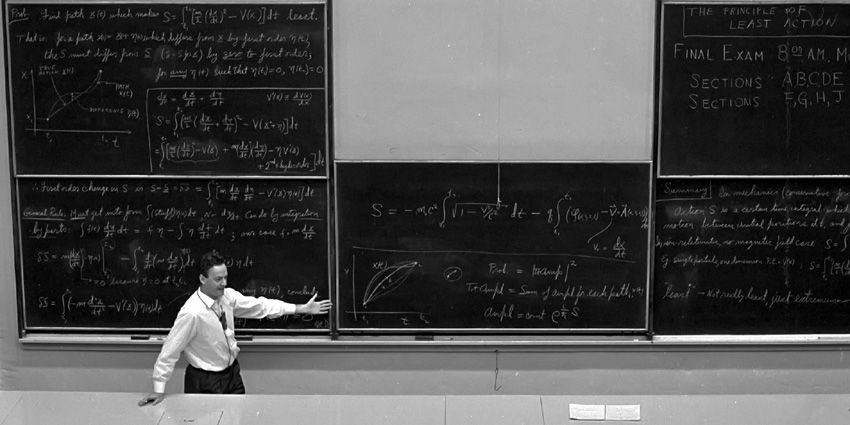
\includegraphics[width=0.7\linewidth]{fyz_fig650.jpg}
      \caption{
               (\cite[s.~707]{Feynman02})}
      \label{fyz_fig650}
    \end{figure}

    \begin{figure}[ht!] %\ref{fyz_fig651}
      \centering
      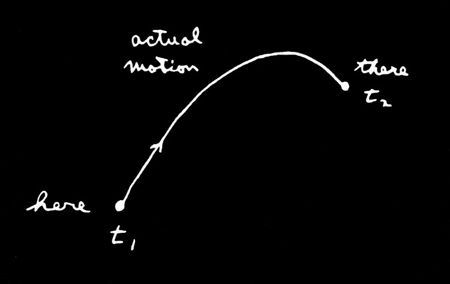
\includegraphics[width=0.7\linewidth]{fyz_fig651.jpg}
      \caption{
               (\cite[s.~707]{Feynman02})}
      \label{fyz_fig651}
    \end{figure}

    \begin{figure}[ht!] %\ref{fyz_fig652}
      \centering
      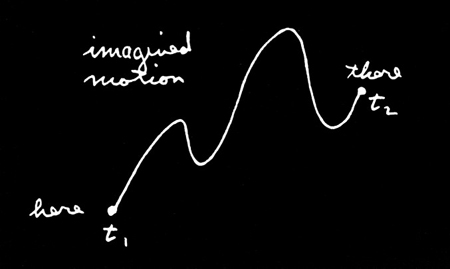
\includegraphics[width=0.7\linewidth]{fyz_fig652.jpg}
      \caption{
               (\cite[s.~707]{Feynman02})}
      \label{fyz_fig652}
    \end{figure}

    \begin{figure}[ht!] %\ref{fyz_fig653}
      \centering
      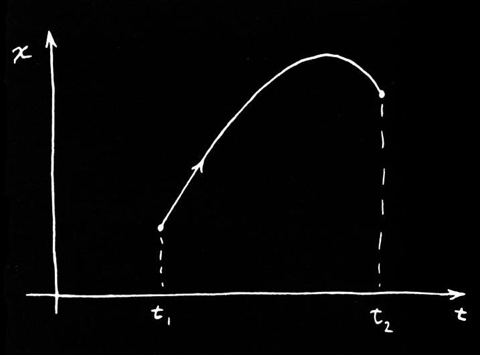
\includegraphics[width=0.7\linewidth]{fyz_fig653.jpg}
      \caption{
               (\cite[s.~707]{Feynman02})}
      \label{fyz_fig653}
    \end{figure}

    \begin{figure}[ht!] %\ref{fyz_fig654}
      \centering
      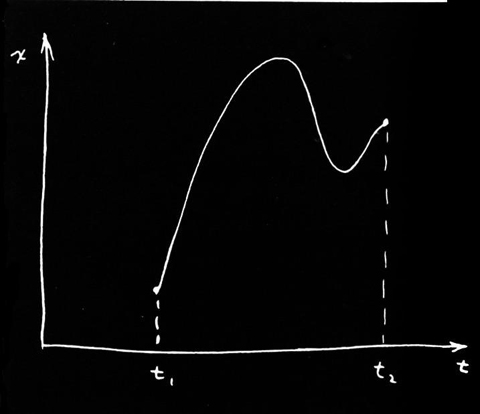
\includegraphics[width=0.7\linewidth]{fyz_fig654.jpg}
      \caption{
               (\cite[s.~707]{Feynman02})}
      \label{fyz_fig654}
    \end{figure}

    \begin{figure}[ht!] %\ref{fyz_fig655}
      \centering
      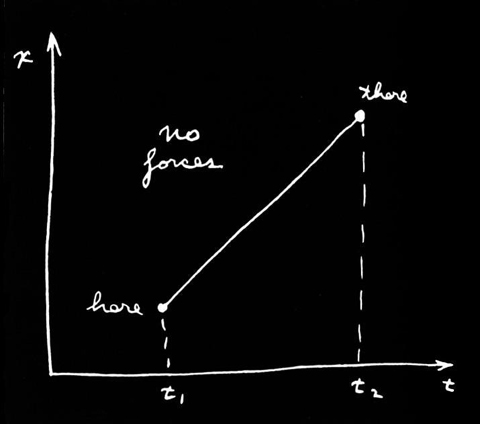
\includegraphics[width=0.7\linewidth]{fyz_fig655.jpg}
      \caption{
               (\cite[s.~707]{Feynman02})}
      \label{fyz_fig655}
    \end{figure}

    \begin{figure}[ht!] %\ref{fyz_fig656}
      \centering
      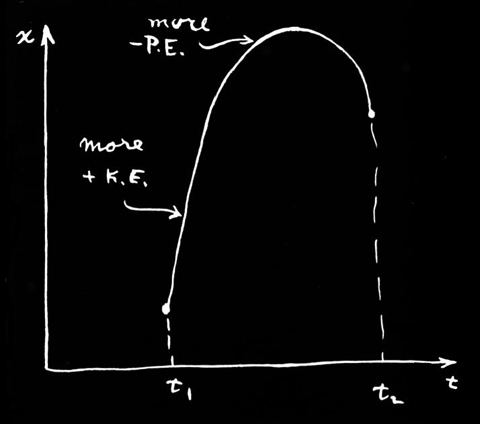
\includegraphics[width=0.7\linewidth]{fyz_fig656.jpg}
      \caption{
               (\cite[s.~707]{Feynman02})}
      \label{fyz_fig656}
    \end{figure}

    \begin{figure}[ht!] %\ref{fyz_fig657}
      \centering
      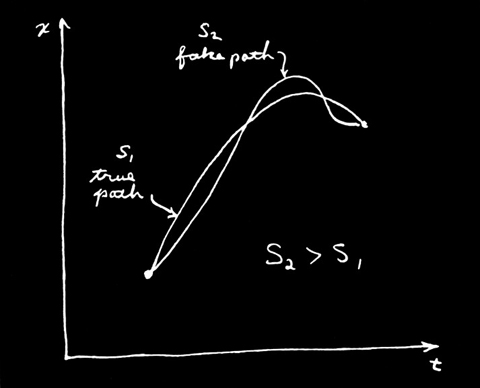
\includegraphics[width=0.7\linewidth]{fyz_fig657.jpg}
      \caption{
               (\cite[s.~707]{Feynman02})}
      \label{fyz_fig657}
    \end{figure}

    \begin{figure}[ht!] %\ref{fyz_fig658}
      \centering
      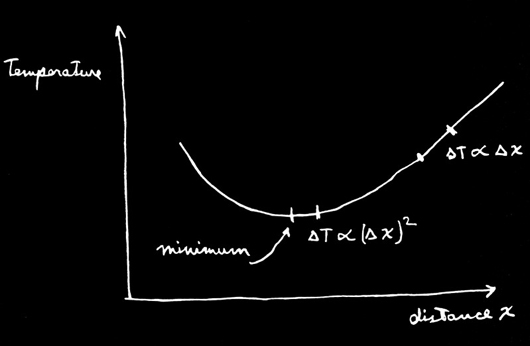
\includegraphics[width=0.7\linewidth]{fyz_fig658.jpg}
      \caption{
               (\cite[s.~707]{Feynman02})}
      \label{fyz_fig658}
    \end{figure}

    \begin{figure}[ht!] %\ref{fyz_fig659}
      \centering
      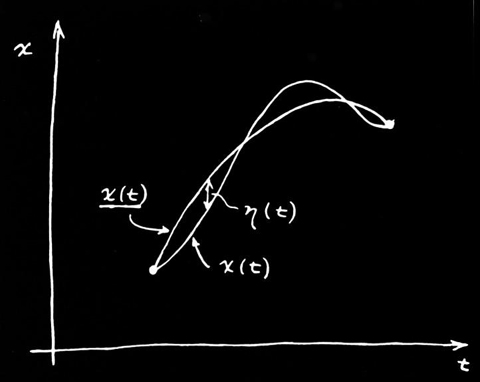
\includegraphics[width=0.7\linewidth]{fyz_fig659.jpg}
      \caption{
               (\cite[s.~707]{Feynman02})}
      \label{fyz_fig659}
    \end{figure}

    \begin{figure}[ht!] %\ref{fyz_fig660}
      \centering
      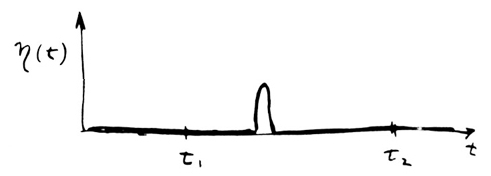
\includegraphics[width=0.7\linewidth]{fyz_fig660.jpg}
      \caption{
               (\cite[s.~707]{Feynman02})}
      \label{fyz_fig660}
    \end{figure}

    \begin{figure}[ht!] %\ref{fyz_fig661}
      \centering
      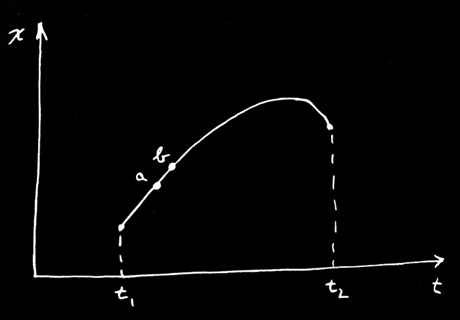
\includegraphics[width=0.7\linewidth]{fyz_fig661.jpg}
      \caption{
               (\cite[s.~707]{Feynman02})}
      \label{fyz_fig661}
    \end{figure}

    \begin{figure}[ht!] %\ref{fyz_fig662}
      \centering
      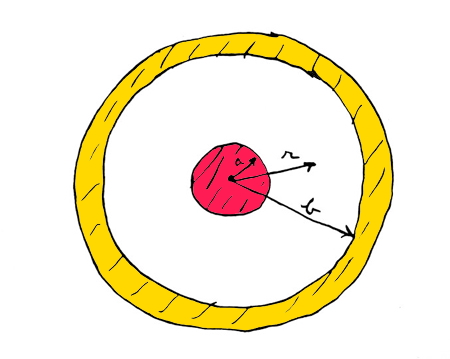
\includegraphics[width=0.7\linewidth]{fyz_fig662.jpg}
      \caption{
               (\cite[s.~707]{Feynman02})}
      \label{fyz_fig662}
    \end{figure}

%} %tikzset
%---------------------------------------------------------------------------------------------------
\printbibliography[title={Seznam literatury},heading=subbibliography]
\addcontentsline{toc}{section}{Seznam literatury}
%==== Kapitola Tenzory =============================================================================
% !TeX spellcheck = cs_CZ
%{\tikzset{external/prefix={tikz/FYZII/}}
% \tikzset{external/figure name/.add={ch31_}{}}
%---------------------------------------------------------------------------------------------------
% file fey2ch31.tex
%---------------------------------------------------------------------------------------------------
%=========================== Kapitola Tenzory ======================================================
\setchaptertoc
\chapter{Tenzory}\label{fyz:IIchapXXXI}

  \section{Tenzory polarizovatelnosti}\label{fyz:IIchapXXXIsecI}
    Fyzici mají ve zvyku zvolit nejednodušší příklad nějakého jevu a nazvat jej „fyzikou", přičemž
    komplikovanější příklady nechávají na starosti jiným odvětvím, například aplikované matematice,
    elektroinženýrství, chemii nebo krystalografii. Dokonce i fyzika pevných látek je téměř
    „polofyzikou”, neboť se příliš zajímá o speciální látky. Proto i v těchto přednáškách budeme
    vynechávat spoustu zajímavých věcí. Například jednou z důležitých vlastností krystalů, nebo
    většiny látek, je to, že jejich elektrická polarizovatelnost je v různých směrech různá.
    Nachází-li se látka ve elektrickém poli, které má určitý směr, posunou se mírně náboje atomů a
    vytvoří se dipólový moment. Velikost tohoto momentu silně závisí na směru pole. A to je,
    samozřejmě, určitá komplikace. Ale ve fyzice si to zjednodušujeme a obvykle začínáme se
    speciálním případem, kdy je polarizovatelnost stejná ve všech směrech. Ostatní případy necháváme
    na starosti jiným vědním oborům. Proto v našich dalších úvahách vůbec nebudeme potřebovat to, o
    čem budeme mluvit v této kapitole.
    
    Matematika tenzorů je zvláště užitečná při popisu těch vlastností látek, které závisejí na
    směru, ačkoliv je to jen jeden z příkladů jejího využití. Jelikož většina z vás se nemíní stát
    fyziky, ale budete se zabývat reálným světem, kde věci silně závisejí na směru, budete muset
    dříve či později používat tenzory. Abychom nic nevynechávali, pohovoříme o tenzorech. Chceme,
    aby naše chápání fyziky bylo co nejúplnější. Například náš výklad elektrodynamiky je úplný - tak
    úplný jako libovolný kurz elektřiny a magnetizmu, dokonce i pro fyzikální specializace na vysoké
    škole. Mechanika nebyla úplně ukončena, protože, když jsme ji probírali, nebyly ještě naše
    matematické znalosti na takové úrovni, abychom mohli hovořit o tématech, jako je princip
    nejmenšího účinku, lagranžiány, hamiltoniány atd., které představují elegantnější způsob popisu
    mechaniky. Ale s výjimkou obecné teorie relativity jsme všechny zákony mechaniky probrali. Naše
    elektřina a magnetizmus jsou kompletní a mnoho dalších oblastí je v podstatě uzavřeno. Kvantová
    mechanika přirozeně ne; musíme si něco nechat do budoucna. Ale co je tenzor, musíme vědět už
    nyní. 

    V kapitole \ref{fyz:IIchapXXX} jsme zdůrazňovali, že vlastnosti krystalických látek jsou v
    různých směrech různé, říkáme, že jsou anizotropní. Závislost indukovaného dipólového momentu na
    směru vnějšího elektrického pole je jen jedním z možných příkladů, ale právě ten si vybereme
    jako příklad tenzoru. Předpokládejme, že při daném směru elektrického pole je indukovaný
    dipólový moment objemové jednotky \(\vec{P}\) úměrný intenzitě vnějšího pole \(\vec{E}\). (To je
    dobrá aproximace pro většinu látek, pokud \(\vec{E}\) není příliš velké.) Konstantu úměrnosti
    označíme \(\alpha\)\footnote{V kapitole \ref{fyz:IIchapX} jsme souhlasně s konvencí psali
    \(P=\varepsilon_0\chi E\) a \(\chi\) („chí") jsme nazývali \emph{susceptibilita}. Nyni bude
    pohodlnější používat jedno písmeno, proto namísto \(\varepsilon_0\chi\) budeme psát \(\alpha\).
    Pro izotropní dielektrika platí \(\alpha = (\varepsilon_r - 1)\varepsilon_0\), kde
    \(\varepsilon_r\) je relativní permitivita (článek \ref{fyz:IIchapXsecIV})}. Budeme uvažovat
    látky, v nichž \(\alpha\) závisí na směru pole, jako například v krystalech podobných vápenci,
    který má tu vlastnost, že při průhledu vidíme obraz dvojitě. 

    Předpokládejme, že jsme zjistili, že v určitém krystalu vyvolává elektrické pole \(\vec{E}_1\),
    působící ve směru osy \(x\), polarizaci \(\vec{P}_1\) ve směru \(x\). Dále nechť elektrické pole
    \(\vec{E}_2\) ve směru osy \(y\), které má stejnou intenzitu jako \(\vec{E}_1\), vyvolává jinou
    polarizaci \(\vec{P}_2\) ve směru \(y\). Co by se stalo, kdyby elektrické pole působilo pod
    úhlem \ang{45}? Takové pole je superpozicí dvou polí působících podél os \(x\) a \(y\), proto
    polarizace \(\vec{P}\) bude vektorovým součtem \(\vec{P}_1\) a \(\vec{P}_2\), jak je znázorněno
    na obr. \ref{fyz:fig0874a}. Polarizace už nemá tentýž směr jako elektrické pole. Lze pochopit,
    proč tomu tak je. V látce se mohou nacházet náboje, které se mohou snadno posouvat směrem nahoru
    a dolů, ale obtížně se pohybují ze strany na stranu. Když síla působí pod úhlem \ang{45}, náboje
    se posunou víc směrem nahoru než na stranu. Výsledné přemístění nemá směr vnější síly, protože
    tu působí vnitřní elastické síly, které jsou asymetrické.
    
    Úhel \ang{45} není, samozřejmě, nijak výjimečný. Indukovaná polarizace obecně nemá směr
    elektrického pole. V našem předcházejícím příkladě se nám „poštěstilo“ zvolit osy \(x\) a \(y\)
    tak, aby \(\vec{P}\) mělo směr \(\vec{E}\) podél obou os. Kdyby byl krystal pootočen vzhledem k
    osám souřadnic, vyvolalo by elektrické pole \(\vec{E}\) ve směru osy \(y\) polarizaci
    \(\vec{P}\), která by měla obě složky, \(x\) i \(y\). Podobně polarizace, která by vznikla díky
    poli ve směru osy \(x\), by také měla složky \(x\) i \(y\). Polarizace by potom vypadaly tak,
    jak je to na obr. \ref{fyz:fig0874b}, a ne jako na obr. \ref{fyz:fig0874a}. Věci se komplikují,
    ale stále je pro libovolné pole \(\vec{E}\) velikost \(\vec{P}\) \emph{úměrná} velikosti
    \(\vec{E}\). 
    
    Nyní uvažujme obecný případ libovolné orientace krystalu vzhledem k souřadnicovým osám.
    Elektrické pole ve směru osy \(x\) vede k polarizaci \(\vec{P}\) se složkami \(x\), \(y\), a
    \(z\). Můžeme psát
    \begin{equation}\label{fyz:eq236}
      P_x = \alpha_{xx}E_x, \quad P_y = \alpha_{yx}E_x, \quad  P_z = \alpha_{zx}E_x.
    \end{equation}

    Celé naše tvrzení je založeno na tom, že má-li elektrické pole směr osy \(x\), nemusí mít
    polarizace tentýž směr, ale má složky ve směru os \(x\), \(y\), \(z\) a každá z nich je úměrná
    \(E_x\). Konstanty úměrnosti označujeme \(\alpha_{xx}\), \(\alpha_{yx}\), \(\alpha_{zx}\).
    (První index je vztažen k příslušné složce \(\vec{P}\), druhý ke směru elektrického pole.) 
    
    Podobně pro pole ve směru osy \(y\) můžeme psát
    \begin{equation}\label{fyz:eq237}
      P_x = \alpha_{xy}E_y, \quad P_y = \alpha_{yy}E_y, \quad  P_z = \alpha_{zy}E_y.
    \end{equation}

    a pro pole ve směru osy \(z\)
    \begin{equation}\label{fyz:eq238}
      P_x = \alpha_{xz}E_z, \quad P_y = \alpha_{yz}E_z, \quad  P_z = \alpha_{zz}E_z.
    \end{equation}

    \begin{figure}[ht!]   %\ref{fyz:fig0874}
      \centering
      \subcaptionbox{\label{fyz:fig0874a}}{\luafigure[0.45]{fyz_fig0874a.pdf}}
      \subcaptionbox{\label{fyz:fig0874b}}{\luafigure[0.45]{fyz_fig0874b.pdf}}
      \caption{Vektorový součet polarizací v anizotropním krystalu (\cite[s.~748]{Feynman02})}
      \label{fyz:fig0874}
    \end{figure}

    Řekli jsme, že polarizace závisí na polích lineárně, proto má-li elektrické pole \(\vec{E}\)
    složku \(x\) i \(y\), bude výsledná \(x\)-ová složka \(\vec{P}\) součtem dvou \(P_x\) z rovnic
    (\ref{fyz:eq236}) a (\ref{fyz:eq237}). Má-li \(\vec{E}\) složky \(x\), \(y\) a \(z\) budou
    výsledné složky \(\vec{P}\) součtem tří příspěvků z rovnic (\ref{fyz:eq236}),
    (\ref{fyz:eq237}), (\ref{fyz:eq238}). Jinými slovy \(\vec{P}\) bude určeno rovnicemi
    \begin{align}\label{fyz:eq240}
      P_x &= \alpha_{xx}E_x + \alpha_{xy}E_y + \alpha_{xz}E_z  \nonumber \\
      P_y &= \alpha_{yx}E_x + \alpha_{yy}E_y + \alpha_{yz}E_z            \\
      P_z &= \alpha_{zx}E_x + \alpha_{zy}E_y + \alpha_{zz}E_z. \nonumber
    \end{align}

    Dielektrické vlastnosti krystalu jsou pak zcela určeny devíti veličinami (\(\alpha_{xx}\),
    \(\alpha_{xy}\), \(\alpha_{xz}\), \(\alpha_{yz}\) \(\ldots\)), které mohou být reprezentovány
    symbolem \(\alpha_{ij}\). (Indexy \(i\), \(j\) zastupují libovolné ze tří písmen \(x\), \(y\),
    \(z\)). Libovolné elektrické pole \(\vec{E}\) může být rozloženo na složky \(E_x\), \(E_y\),
    \(E_z\). Z nich můžeme použitím \(\alpha_{ij}\) najít \(P_x\), \(P_y\) a \(P_z\), které nám
    spolu určují polarizaci \(\vec{P}\). Soubor devíti koeficientů \(\alpha_{ij}\) se nazývá
    \textbf{tenzor} - v tomto případě \textbf{tenzor polarizovatelnosti}. Když říkáme, že tři čísla
    (\(E_x\), \(E_y\), \(E_z\)) tvoří vektor \(\vec{E}\), stejně říkáme, že devět čísel
    (\(\alpha_{xx}\), \(\alpha_{xy}\), \(\alpha_{xz}\), \(\alpha_{yz}\) \(\ldots\)) tvoří tenzor
    \(\alpha_{ij}\). 

  \twocolumn[\section{Transformace tenzorových složek}\label{fyz:IIchapXXXIsecII}]
    Víme, že při přechodu k nové souřadnicové soustavě \(x'\), \(y'\), \(z'\) dostáváme jiné složky
    \(E_{x'}\), \(E_{y'}\),  \(E_{z'}\) vektoru \(\vec{E}\) a stejně i jiné \emph{složky} vektoru
    \(\vec{P}\). Proto všechny koeficienty \(\alpha_{ij}\) mají různou hodnotu v různých
    souřadnicových soustavách. Změnu koeficientů \(\alpha\) při změně \(\vec{E}\) a \(\vec{P}\) lze
    zjistit, neboť popisujeme-li \emph{stejné fyzikální} elektrické pole v nové souřadnicové
    soustavě, měli bychom dostat stejnou polarizaci. Pro libovolnou novou souřadnicovou soustavu je
    \(P_{x'}\) lineární kombinací \(P_{x}\), \(P_{y}\), a \(P_{z}\):
    \begin{equation*}
      P_{x'} = aP_x + bP_y + cP_z.
    \end{equation*}
    Podobně je to i pro ostatní složky. Dosadíme-li za \(P_{x}\), \(P_{y}\), a \(P_{z}\), jejich
    vyjádření pomocí \(\vec{E}\) rovnic (\ref{fyz:eq240}), dostaneme
    \begin{align*}
      P_{x'} = &a(\alpha_{xx}E_x + \alpha_{xy}E_y + \alpha_{xz}E_z) + \\
               &b(\alpha_{yx}E_x + \alpha_{yy}E_y + \alpha_{yz}E_z) + \\
               &c(\alpha_{zx}E_x + \alpha_{zy}E_y + \alpha_{zz}E_z).
    \end{align*}
    Pak vyjádříme \(E_{x}\), \(E_{y}\), a \(E_{z}\), pomocí \(E_{x'}\), \(E_{y'}\), a \(E_{z'}\),
    například
    \begin{equation*}
      E_x =  a'E_x + b'E_y + c'E_z,
    \end{equation*}
    kde \(a'\), \(b'\), \(c'\) jsou v nějakém vztahu k \(a\), \(b\), \(c\), ale navzájem si nejsou
    rovny. Vyjádřili jsme tedy \(P_{x'}\) pomocí složek \(E_{x'}\), \(E_{y'}\), a \(E_{z'}\), tj.
    máme nové \(\alpha_{ij}\). To je trochu neuspořádaný, ale přímočarý postup.

    Když mluvíme o změně os, předpokládáme, že poloha krystalu v prostoru je fixována. Kdyby se
    krystal otáčel \emph{společně} s osami, koeficienty \(\alpha\) by se neměnily. Naopak, kdyby se
    orientace krystalu vzhledem k osám změnila, dostali bychom nový soubor hodnot \(\alpha\).
    Známe-li však koeficienty \(\alpha\) pro nějakou libovolnou orientaci krystalu, můžeme je najít
    pro libovolnou jinou orientaci pomocí transformace, kterou jsme právě popsali. Jinými slovy,
    dielektrické vlastnosti jsou \emph{úplně} popsány zadáním složek polarizovatelnosti tenzoru
    \(\alpha_{ij}\) vzhledem k libovolně zvolené soustavě souřadnic. Stejně jako částici přiřazujeme
    vektor rychlosti \(\vec{v} = (v_x, v_y, v_z)\), vědomi si toho, že tři složky se určitým
    způsobem mění při změně souřadnicových os, podobně krystalu přiřazujeme tenzor
    polarizovatelnosti \(\alpha_{ij}\), jehož devět složek se při změně souřadnicové soustavy
    transformuje určitým způsobem.

    Vztah mezi \(\vec{P}\) a \(\vec{E}\) určený rovnicí (\ref{fyz:eq240}) můžeme zapsat ve zkráceném
    tvaru
    \begin{equation}\label{fyz:eq241}
      P_i = \sum_j\alpha_{ij}E_j,
    \end{equation}

    kde \(i\) označuje některé z písmen \(x\), \(y\) nebo \(z\) a sčítáme přes \(j = x, y, z\). Pro
    operace s tenzory bylo vynalezeno mnoho speciálních označení, ale každé z nich se hodí jen pro
    omezenou třídu problémů. Jednou z obecných konvencí je vynechávání sumačního znaku \(\sum\) v
    rovnici (\ref{fyz:eq241}), přičemž se rozumí, že všude, kde se stejný index vyskytuje dvakrát (v
    našem případě \(j\)), musíme sčítat přes všechny jeho hodnoty. Jelikož tenzory nebudeme používat
    často, nebudeme se trápit s výběrem speciálních označení a konvencí.

  \section{Elipsoid energie}\label{fyz:IIchapXXXIsecIII}
    Nyní si vyzkoušejme, jak se zachází s tenzory. Položíme si zajímavou otázku: Jaká energie je
    potřebná k polarizaci krystalu (kromě energie elektrického pole, o níž víme, že je rovna
    \(\varepsilon_0E^2/2\) pro objemovou jednotku)? Zamyslíme se nad atomovými náboji, které se
    posouvají. Práce, která je vykonána při přemisťování náboje o vzdálenost \(\dd{x}\), je
    \(qE_x\dd{x}\) a je-li v jednotkovém objemu \(N\) nábojů, je vykonaná práce  \(qE_xN\dd{x}\).
    Ale  \(qN\dd{x}\) je změna \(qP_x\), dipólového momentu objemové jednotky. Proto energie
    připadající na \emph{objemovou jednotku} je
    \begin{equation*}
      E_x\dd{P_x}.
    \end{equation*}

    Sečteme-li práci všech tří složek pole, pro práci připadající na objemovou jednotku dostaneme
    \begin{equation*}
      \vec{E}\cdot\dd{P}.
    \end{equation*}
    Jelikož velikost \(\vec{P}\) je úměrná \(\vec{E}\), bude práce vykonaná při polarizování
    objemové jednotky od 0 do \(\vec{P}\) rovna integrálu výrazu \(\vec{E}\cdot\dd{P}\). Označíme-li
    tuto práci \(\omega_p\), můžeme psát\footnote{Je to práce spotřebovaná na vytvoření polarizace
    elektrickým polem a není možné ji zaměňovat s potenciální energií \(-\vec{p}_o\cdot\vec{E}\).
    konstantního dipólového momentu \(\vec{p}_o\).}
    \begin{equation}\label{fyz:eq242}
      \omega_p = \frac{1}{2}\vec{E}\cdot\vec{P} = \frac{1}{2}\sum_iE_iP_i.
    \end{equation}

    Nyní můžeme vyjádřit \(\vec{P}\) pomocí \(\vec{E}\) použitím rovnice (\ref{fyz:eq241}) a
    dostaneme
    \begin{equation}\label{fyz:eq243}
      \omega_p = \frac{1}{2}\sum_i\sum_j\alpha_{ij}E_iE_j.
    \end{equation}
    Hustota energie \(w_p\), je číslo, které nezávisí na výběru os, je to tedy skalár. Tenzor
    \(\alpha_{ij}\) bychom měli správně nazývat tenzor druhého řádu, neboť má dva indexy. Vektor (s
    \emph{jedním} indexem je tenzor prvního řádu a skalár (bez indexu) je tenzor nultého řádu.
    Říkáme, že elektrické pole \(\vec{E}\) je tenzor prvního řádu a že hustota energie \(w_p\) je
    tenzor nultého řádu. Pojem tenzoru bychom mohli rozšířit na tři a víc indexů, a tak bychom
    sestrojili tenzory vyššího než druhého řádu.

    Indexy tenzoru polarizovatelnosti mohou nabývat tří různých hodnot - je to trojrozměrný tenzor.
    Matematici uvažují tenzory ve čtyřech, pěti nebo vyšších rozměrech. My jsme už používali
    čtyřrozměrný tenzor \(\vec{F}_{\mu\nu}\), při našem relativistickém popisu elektromagnetického
    pole (kapitola \ref{fyz:IIchapXXVI}).

    \luagraphic[0.8]{fyz_fig0875.pdf}{Množina koncových bodů vektoru \(\vec{E} = (E_x, E_y)\), který
    odpovídá konstantní energii polarizace (\cite[s.~577]{Feynman02})}{fyz:fig0875}

    Tenzor polarizovatelnosti \(\alpha_{ij}\) má tu zajímavou vlastnost, že je symetrický, to
    znamená, že \(\alpha_{xy} = \alpha_{yx}\), a totéž platí pro libovolnou dvojici indexů. (To je
    \emph{fyzikální} vlastnost reálného krystalu, a neplatí nevyhnutelně pro všechny tenzory.)
    Můžete si sami dokázat, že to tak musí být, výpočtem změny energie krystalu následujícím
    postupem: 1. Zapněte elektrické pole ve směru osy \(x\). 2. Zapněte pole ve směru osy \(y\). 3.
    Vypněte pole ve směru osy \(x\). 4. Vypněte pole ve směru osy \(y\).

    Krystal je nyní v takovém stavu, jako byl na začátku, a celková práce spotřebovaná na polarizaci
    musí být rovna nule. Lze však ukázat, že má-li to být pravda, musí být \(\alpha_{xy}\), rovno
    \(\alpha_{yx}\). Stejné úvahy můžeme, samozřejmě, aplikovat i na \(\alpha_{xz}\), atd.
    \emph{Tenzor polarizovatelnosti je tedy symetrický}.

    To také znamená, že tenzor polarizovatelnosti můžeme určit změřením energie potřebné k
    polarizaci krystalu v různých směrech. Předpokládejme, že pole \(\vec{E}\) působí jen ve směru
    os \(x\) a \(y\). Pak souhlasně s rovnicí (\ref{fyz:eq243}) pro \(\omega_p\) dostáváme
    \begin{equation}\label{fyz:eq244}
      \frac{1}{2}\left(\alpha_{xx}E_x^2 + (\alpha_{xy} + \alpha_{yx})E_xE_y + \alpha_{yy}E_y^2\right).
    \end{equation}

    Kdybychom měli jen složku \(E_x\), mohli bychom určit \(\alpha_{xx}\) v případě složky \(E_y\)
    můžeme určit \(\alpha_{yy}\), máme-li zároveň \(E_x\) i \(E_y\), dostáváme energii pocházející
    ze členu s \(\alpha_{xy} + \alpha_{yx}\). Jelikož \(\alpha_{xy}\) a \(\alpha_{yx}\) jsou si
    navzájem rovny, je tento člen úměrný \(2\alpha_{xy}\) a lze jej určit z energie.

    výraz pro energii \eqref{fyz:eq244} má pěknou geometrickou interpretaci. Předpokládejme, že se
    ptáme, jaká pole \(E_x\) a \(E_y\) odpovídají dané hustotě energie, například \(\omega_0\). Je
    to matematická úloha řešení rovnice:
    \begin{equation*}
      \alpha_{xx}E_x^2 + 2\alpha_{xy}E_xE_y + \alpha_{yy}E_y^2 = 2\omega_0.
    \end{equation*}

    To je \emph{kvadratická rovnice}, proto při grafickém znázornění této rovnice (obr.
    \ref{fyz:fig0875}) budou všechna řešení \(E_x\) a \(E_y\) ležet na elipse. (Musí to být elipsa, a
    ne parabola nebo hyperbola, neboť energie je pro libovolné pole vždy kladná a konečná.) Vektor
    \(\vec{E}\) se složkami \(E_x\) a \(E_y\) bude znázorněn tak, že jeho počátek je v počátku
    souřadnic a koncový bod leží na elipse. Pomocí této „energetické elipsy“ názorně vidíme jak
    „vypadá“ polarizační tenzor.

    \luagraphic[0.7]{fyz_fig0876.pdf}{Elipsoid energie tenzoru polarizovatelnosti
    (\cite[s.~577]{Feynman02})}{fyz:fig0876}
    
    Vezmeme-li nyní v úvahu všechny tři složky vektoru \(\vec{E}\) libovolného směru, který vede k
    jednotkové hustotě energie, budou jeho koncové body ležet na povrchu \textbf{elipsoidu}, jak je
    to na obr. \ref{fyz:fig0876}. Tvar tohoto elipsoidu konstantní energie jednoznačně určuje tenzor
    polarizovatelnosti.

    Elipsoid má pěknou vlastnost, že vždy může být popsán prostě zadáním směrů tří hlavních os a
    průměry elipsoidu podél těchto os. Hlavní osy - osy ve směru nejdelšího a nejkratšího průměru a
    ve směru kolmém na obě tyto osy. Na obr. \ref{fyz:fig0876} jsou označeny jako \(a\), \(b\),
    \(c\). Vzhledem k těmto osám nabývá rovnice elipsoidu obzvlášť jednoduchého tvaru
    \begin{equation*}
      \alpha_{aa}E_a^2 + \alpha_{bb}E_b^2 + \alpha_{cc}E_c^2= 2\omega_0.
    \end{equation*}

    Tenzor polarizovatelnosti má tedy jen tři nenulové složky: \(\alpha_{aa}\), \(\alpha_{bb}\) a
    \(\alpha_{cc}\). To znamená, že pro libovolně komplikovaný krystal je vždy možné vybrat jen
    takové osy (nemusí to být osy krystalu), pro které má náš tenzor jen tři složky. Pro takové osy
    nabývají rovnice \eqref{fyz:eq240} jednoduchý tvar
    \begin{equation}\label{fyz:eq832}
      P_a = \alpha_{aa}E_a,\quad P_b = \alpha_{bb}E_b,\quad P_a = \alpha_{cc}E_c.
    \end{equation}
    Elektrické pole podél jedné z hlavních os vyvolává polarizaci podél téže osy, ale, samozřejmě,
    koeficienty, které patří třem osám, mohou být různé.

    Tenzor často píšeme jako tabulku devíti koeficientů uvnitř závorek
    \begin{equation}\label{fyz:eq938} 
      \begin{bmatrix}
        \alpha_{xx}& \alpha_{xy}& \alpha_{xz} \\
        \alpha_{yx}& \alpha_{yy}& \alpha_{yz} \\
        \alpha_{zx}& \alpha_{zy}& \alpha_{zz}
      \end{bmatrix}.
    \end{equation}

    Pro hlavní osy \(a\), \(b\), \(c\) jsou jen diagonální členy různé od nuly. Říkáme, že tenzor je
    diagonální a jeho tvar je
    \begin{equation}\label{fyz:eq939}
      \begin{bmatrix}
        \alpha_{aa}&      0      &      0      \\
             0     & \alpha_{bb} &      0      \\
             0     &      0      & \alpha_{cc}
      \end{bmatrix}.
    \end{equation}
    Důležitým faktorem je, že libovolný tenzor polarizovatelnosti (ve skutečnosti libovolný
    symetrický tenzor druhého stupně pro libovolný počet rozměrů) se může v tomto tvaru psát při
    vhodném výběru souřadnicových os.
    
    Jsou-li si tři prvky polarizačního vektoru v diagonálním tvaru rovny,
    \begin{equation}\label{fyz:eq940}
        \alpha_{aa} = \alpha_{bb} = \alpha_{cc} = \alpha,
    \end{equation}
    stává se \emph{elipsoid energie kulovou plochou} a polarizovatelnost je stejná ve všech směrech.
    Látka je \emph{izotropní}. V tenzorovém označení
    \begin{equation}\label{fyz:eq946}
      \alpha_{ij} = \alpha\delta_{ij},
    \end{equation}
    kde \(\delta_{ij}\) je \textbf{jednotkový tenzor}
    \begin{equation}\label{fyz:eq942}
      \delta_{ij} = 
      \begin{bmatrix}
             1 & 0 & 0 \\
             0 & 1 & 0 \\
             0 & 0 & 1  
      \end{bmatrix}.
    \end{equation}
    To samozřejmě znamená, že
    \begin{equation}\label{fyz:eq943}
      \delta_{ij} = 
      \begin{cases} 
         1  & \text{pro } i = j     \\
         0  & \text{pro } i \neq j.
      \end{cases}
    \end{equation}

    Tenzor \(\delta_{ij}\) se často nazývá \textbf{Kroneckerovo delta}. Můžeme se pobavit tím, že
    dokážeme, že tenzor \eqref{fyz:eq942} bude mít po záměně jedné pravoúhlé soustavy za druhou
    přesně tutéž formu. Tenzor polarizovatelnosti typu \eqref{fyz:eq946} nám dává
    \begin{equation*}
      P_i = \alpha\sum_j\delta_{ij}E_j = \alpha E_i,
    \end{equation*}
    což je totéž jako náš starý výsledek pro izotropní dielektrika
    \begin{equation*}
      \vec{P} = \alpha\vec{E},
    \end{equation*}

    Tvar a orientace elipsoidu polarizovatelnosti může někdy souviset s vlastnosti symetrie
    krystalu. V kapitole \ref{fyz:IIchapXXX} jsme řekli, že existuje 230 různých možných symetrií
    trojrozměrné mřížky a pro různé účely je vhodné je rozdělit na sedm tříd podle tvaru základní
    buňky. Elipsoid polarizovatelnosti musí odrážet vnitřní symetrii krystalu. Například trojklonný
    krystal má nízkou symetrii - elipsoid polarizovatelnosti bude mít nestejné osy a jejich
    orientace nebude obecně souhlasit se směrem os krystalu. Na druhé straně má jednoklonná mřížka
    tu vlastnost, že při rotaci o \ang{180} kolem jedné osy se její vlastnosti nemění. Proto
    polarizační tenzor musí při takové rotaci zůstávat nezměněn. Z toho vyplývá, že tenzor
    polarizovatelnosti se po rotaci o \ang{180} musí transformovat sám v sebe. To je možné jen v tom
    případě, kdy jedna z os elipsoidu má tentýž směr jako osa symetrie krystalu. Žádná další omezení
    na orientaci a rozměry elipsoidu nejsou.
    
    Pro kosočtverečný krystal však musí osy elipsoidu souhlasit s osami krystalu, neboť při rotaci o
    \ang{180} kolem libovolné ze tří os dostáváme tutéž mřížku. Vezmeme-li čtverečný krystal, musí
    mít elipsoid stejnou symetrii, tj. musí mít dva průměry stejné. Nakonec, pro krychlový krystal
    musí být všechny tři průměry elipsoidu stejné. Elipsoid se stává kulovou plochou a
    polarizovatelnost krystalu je ve všech směrech stejná.
    
    Existuje celá věda o určování druhů tenzorů pro všechny možné symetrie krystalu. Je to analýza
    založená na teorii grup. Ale pro jednoduché případy tenzoru polarizovatelnosti je poměrně snadno
    vidět, jaké musí příslušné vztahy být.

  \section{Tenzor setrvačnosti}\label{fyz:IIchapXXXIsecIV} 
  
    Ve fyzice najdeme mnohé další příklady tenzorů. Například v kovu nebo v libovolném vodiči bývá
    často proudová hustota \(\vec{j}\) přibližně úměrná elektrickému poli \(\vec{E}\). Konstanta
    úměrnosti a se nazývá měrná \emph{vodivost} (konduktivita):
    \begin{equation*}
      \vec{j} = \sigma\vec{E}.
    \end{equation*}
    Pro krystaly je však vztah mezi \(\vec{j}\) a \(\vec{E}\) mnohem komplikovanější, vodivost není
    stejná ve všech směrech. Konduktivita je tenzorem, proto píšeme
    \begin{equation*}
      j_i = \sum_j\sigma_{ij}E_j
    \end{equation*}

    Dalším příkladem fyzikálního tenzoru je moment setrvačnosti. V \ref{fyz:IchapXVIII}. kapitole
    \ref{part:FYZI}. dílu jsme viděli, že při rotaci tuhého tělesa kolem fixované osy jejeho moment
    hybnosti \(L\) úměrný úhlové rychlosti \(ω\) a koeficient úměrnosti \(L\) jsme nazvali
    \emph{momentem setrvačnosti} \[L=I\omega\].

    Moment setrvačnosti libovolně tvarovaného tělesa závisí na jeho orientaci vzhledem k ose
    otáčení. Například kvádr bude mít různé momenty vzhledem ke každé z jeho tří navzájem kolmých
    os. Úhlové rychlosti \(\vec{ω}\) i moment hybnosti \(\vec{L}\) jsou vektory. Při rotaci kolem
    jedné z os symetrie jsou tyto vektory rovnoběžné. Avšak jsou-li momenty setrvačnosti vzhledem ke
    třem hlavním osám různé, nemusí být \(\vec{ω}\) a \(\vec{L}\) vždy rovnoběžné (obr.
    \ref{fyz:fig0877}). Jejich vzájemný vztah je podobný jako vztah mezi \(\vec{E}\) a \(\vec{P}\).
    Obecně musíme psát
    \begin{align}
      Lx&=I_{xx}=I_{xx}ω_x+I_{xy}ω_y+I_{xz}ω_z,  \nonumber         \\
      Ly&=I_{yx}=I_{yx}ω_x+I_{yy}ω_y+I_{yz}ω_z,  \label{fyz:eq944} \\
      Lz&=I_{zx}=I_{zx}ω_x+I_{zy}ω_y+I_{zz}ω_z.  \nonumber 
    \end{align}
    Devět koeficientů \(I_{ij}\). je nazýváno \textbf{tenzor setrvačnosti}. Podobně jako v případě
    polarizace musí být kinetická energie pro libovolný moment hybnosti kvadratickou formou vzhledem
    k \(ω_x\), \(ω_y\) a \(ω_z\):
    \begin{equation}\label{fyz:eq945}
      E_k = \frac{1}{2}\sum_{ij}L_{ij}ω_iω_j.
    \end{equation}
    Energii můžeme využít k definování \textbf{elipsoidu setrvačnosti}. Opět můžeme pomocí úvah o
    energii dokázat, že tenzor setrvačnosti je \emph{symetrický}, tj. že \(I_{ij} = I_{ji}\)

    Tenzor setrvačnosti tuhého tělesa můžeme určit, zname-li jeho tvar. Potřebujeme jen napsat
    kinetickou energii všech částic tělesa. Částice, která má hmotnost \(m\) a rychlost \(\vec{v}\),
    má kinetickou energii \(\sfrac{1}{2}mv^2\) a celková kinetická energie je součtem výrazů
    \[\sum\frac{1}{2}mv^2\] pocházejících od všech částic tělesa. Rychlost \(\vec{v}\) každé částice
    souvisí s úhlovou rychlostí \(\vec{ω}\) tuhého tělesa. Předpokládejme, že těleso se otáčí kolem
    svého těžiště, které je v klidu. Je-li \(\vec{r}\) polohový vektor částice vzhledem k těžišti,
    rychlost částice \(\vec{v}\) je dána výrazem \(\vec{ω}\times\vec{r}\). Celková kinetická energie
    je
    \begin{equation}\label{fyz:eq948}
      E_k = \sum\frac{1}{2}m\left(\vec{ω}\times\vec{r}\right)^2.
    \end{equation}

    \luagraphic[0.7]{fyz_fig0877.pdf}{Moment hybnosti \(\vec{L}\) tuhého tělesa obecně není
    rovnoběžný s úhlovou rychlostí \(\vec{ω}\) (\cite[s.~580]{Feynman02})}{fyz:fig0877}
    
    Nyní už jen stačí rozepsat \(\vec{ω}\times\vec{r}\) pomocí složek \(ω_x\), \(ω_y\) a \(ω_z\) a
    \(x\), \(y\), \(z\) a porovnat výsledek s rovnicí \eqref{fyz:eq945}. \(I_{ij}\) najdeme
    porovnáním jednotlivých členů. Provedeme algebraické úpravy
    \begin{equation*}
      (\vec{ω}×\vec{r})^2=(\vec{ω}×\vec{r})^2_x+(\vec{ω}×\vec{r})^2_y+(\vec{ω}×\vec{r})^2_z
    \end{equation*}
    čili
    \begin{equation*}
      (ω_yz−ω_zy)^2+(ω_zx−ω_xz)^2+(ω_xy−ω_yx)^2
    \end{equation*}
    a konečně
    \begin{align*}
      = &+ω_y^2z − 2ω_yω_z zy + ω_z^2y^2 \\
        &+ω_z^2x − 2ω_zω_x xz + ω_x^2z^2 \\
        &+ω_x^2y − 2ω_xω_y yx + ω_y^2x^2.
    \end{align*}
    Vynásobřme-li tuto rovnici veličinou \(\sfrac{m}{2}\) sečteme přes všechny částice a porovnáme s
    rovnicí \eqref{fyz:eq945}, zjistíme, že například \(I_{xx}\) je rovno
    \begin{equation*}
      I_{xx}=∑m(y^2+z^2).
    \end{equation*}
    Je to tentýž vzorec, který jsme dostali v \ref{fyz:IchapXIX}. kapitole \ref{part:FYZI}. dílu pro
    moment setrvačnosti tělesa vzhledem k ose \(x\). Jelikož \(r^2 = x^2 + y^2 + z^2\) můžeme tento
    vzorec psát i jako
    \begin{equation*}
      I_{xx}=∑m(r^2-x^2).
    \end{equation*}
    Vypíšeme-li všechny ostatní členy tenzoru setrvačnosti \(I_{ij}\), dostaneme
    \begin{equation*}
      \begin{bmatrix}
        \sum m(r^2-x^2) &    -\sum mxy     &   -\sum mxz     \\
          -\sum myx     &  \sum m(r^2-y^2) &   -\sum myz     \\
          -\sum mzx     &    -\sum mzy     & \sum m(r^2-z^2)
      \end{bmatrix}.
    \end{equation*}
    Chceme-li, můžete si to zapsat v tenzorovém označení jako
    \begin{equation}\label{fyz:eq949}
      I_{ij}=\sum m(r^2\delta_{ij}-r_ir_j),
    \end{equation}
    kde \(r_i\) jsou složky \((x, y, z)\) polohového vektoru částice a \(\sum\) označuje sumu přes
    všechny částice. \emph{Moment setrvačnosti je tedy tenzorem druhého řádu}. Jeho členy jsou
    určeny vlastnostmi tělesa a vztah mezi \(\vv{L}\) a \(\vv{\omega}\) je vyjádřen pomocí tohoto
    tenzoru jako
    \begin{equation}\label{fyz:eq950}
      L_i=\sum_jI_{ij}\omega_j.
    \end{equation}
    Pro těleso libovolného tvaru lze najít elipsoid setrvačnosti, a tedy i tři hlavní osy. Vzhledem
    k těmto osám bude tenzor diagonální, tj. pro libovolný objekt existují vždy tři navzájem kolmé
    osy, pro něž jsou úhlová rychlost a moment hybnosti paralelní. Nazývají se \textbf{hlavní osy
    setrvačnosti}.

  \section{Vektorový součin}\label{fyz:IIchapXXXIsecV}   
    Vzpomeňme si, že tenzory druhého řádu jsme používali už od \ref{fyz:IchapXX}. kapitoly
    \ref{part:FYZI}. dílu. Tehdy jsme definovali \emph{moment síly v rovině}, například složku
    \(N_{xy}\) vztahem 
    \begin{equation*}
      N_{xy} = xF_y-yF_x.
    \end{equation*}
    Po zobecnění na tři rozměry lze psát
    \begin{equation}\label{fyz:eq947}
      N_{ij} = r_iF_j-r_jF_i.
    \end{equation}
    Veličina \(N_{ij}\) je \emph{tenzor druhého řádu}. Lze to ukázat například tak, že zkombinujeme
    \(N_{ij}\) s nějakým vektorem, řekněme s jednotkovým vektorem \(\vec{e}\), tímto způsobem:
    \begin{equation*}
      \sum_jN_{ij}e_j.
    \end{equation*}
    Je-li takováto veličina \emph{vektor}; musí se \(N_{ij}\) transformovat jako tenzor - to je naše
    definice tenzoru. Dosadíme za \(N_{ij}\) a dostaneme
    \begin{align*}
      \sum_jN_{ij}e_j
        &=\sum_jr_iF_je_j-\sum_jr_je_jF_i           \\[1ex]
        &=r_i(\vec{F}\cdot\vec{e})-(\vec{r}\cdot\vec{e})F_i.
    \end{align*}
    Jelikož skalární součin je skalár, jsou dva členy na pravé straně rovnice vektory a vektorem je
    i jejich rozdíl. \(N_{ij}\) je tedy tenzor.

    Ale \(N_{ij}\) je speciálním druhem tenzoru - je to \textbf{antisymetrický tenzor}, pro nějž
    platí
    \begin{equation*}
      N_{ij}=-N_{ji},
    \end{equation*}
    tj. má jen tři nenulové členy \(-N_{xy}\), \(N_{yz}\) a \(N_{zx}\). V \ref{fyz:IchapXX}.
    kapitole \ref{part:FYZI}. dílu se nám podařilo ukázat, že tyto tři členy se téměř \uv{náhodou}
    transformují jako tři složky vektoru, takže jsme mohli \emph{definovat}
    \begin{equation*}
      N = N_{ij}=-N_{ji},
    \end{equation*}
    
    Říkáme „náhodou“, neboť toto platí jen v trojrozměrném případě. Pro čtyři rozměry má například
    antisymetrický tenzor druhého řádu šest nenulových složek a, samozřejmě, nemůže být nahrazen
    vektorem se čtyřmi složkami.
    \begin{equation*}
      \vec{N}=(N_x,N_y,N_z)=(N_{yz},N_{zx},N_{xy})
      \end{equation*}
    Stejně jako axiální vektor \(\vec{N}=\vec{r}\times\vec{F}\) je tenzorem, i každý vektorový
    součin dvou polárních vektorů je tenzorem. Lze použít stejné argumenty. Naštěstí je možné je
    psát jako vektory (přesněji pseudovektory), což nám zjednodušuje naši matematiku.
    
    Matematicky, jsou-li \(\vec{a}\) a \(\vec{b}\) libovolné dva vektory, tvoří devět veličin
    \(a_ib_j\) tenzor (ačkoliv nemusí mít žádný fyzikální význam). Tak dostáváme z polohového
    vektoru \(r_i\). tenzor \(r_ir_j\) a jelikož \(\delta_{ij}\) je také tenzor, je pravá strana
    rovnice \eqref{fyz:eq949} tenzor. Podobně rovnice \eqref{fyz:eq947} je tenzor, jelikož oba členy
    na pravé straně jsou tenzory.

  \section{Tenzor napětí}\label{fyz:IIchapXXXIsecVI} 

    Symetrické tenzory, s nimiž jsme se dosud setkali, vznikly z koeficientů, které dávaly do
    vzájemného vztahu dva vektory. Nyní se seznámíme s tenzorem, který má jiný fyzikální význam - s
    \textbf{tenzorem napětí}. Předpokládejme, že máme pevné těleso, na nějž působí různé síly.
    Říkáme, že uvnitř působí různá „napětí“, čímž rozumíme, že mezi sousedními částicemi látky
    působí vnitřní síly. O takových napětích jsme se zmínili už v článku \ref{fyz:IIchapXIIsecIII},
    když jsme uvažovali dvojrozměrný případ povrchového napětí napnuté membrány. Nyní si ukážeme, že
    vnitřní síly působící v látce trojrozměrného tělesa mohou být popsány pomocí tenzoru.

    \begin{figure}[ht!] %\ref{fyz:fig0878}
      \centering
      \subcaptionbox{\label{fyz:fig0878a}}{\luafigure[0.45]{fyz_fig0878a.pdf}}
      \subcaptionbox{\label{fyz:fig0878b}}{\luafigure[0.45]{fyz_fig0878b.pdf}}
      \caption{Látka nalevo od roviny \(\sigma\) působí přes plošku \(\Delta x\Delta y\) silou
              \(\Delta F_1\), na látku napravo (\cite[s.~583]{Feynman02})}
      \label{fyz:fig0878}
    \end{figure}

    Uvažujme těleso z nějakého pružného materiálu, například kostku želatiny. Když je rozřízneme,
    látka se na obou stranách řezu působením vnitřních sil posune. Předtím, než jsme řez provedli,
    musely mezi oběma částmi kostky existovat síly, které udržovaly látku pohromadě: napětí můžeme
    definovat pomocí těchto sil. Představme si rovinu kolmou na osu \(x\) (jako je rovina \(\sigma\)
    na obr. \ref{fyz:fig0879}) a ptáme se na síly působící na malou plošku \(\Delta y\Delta z\) této
    roviny. Látka nalevo od plošky působí silou \(Δ\vec{F_1}\) na látku napravo tak, jak je
    znázorněno na obrázku \ref{fyz:fig0878b}. Na látku nalevo od plochy působí, samozřejmě, opačná
    síly reakce \(-Δ\vec{F_1}\). Je-li ploška dostatečně malá, očekáváme, že síla \(Δ\vec{F_1}\)? je
    úměrná velikosti plochy \(\Delta y\Delta z\).

    \begin{figure}[ht!] %\ref{fyz:fig0879}
      \centering
      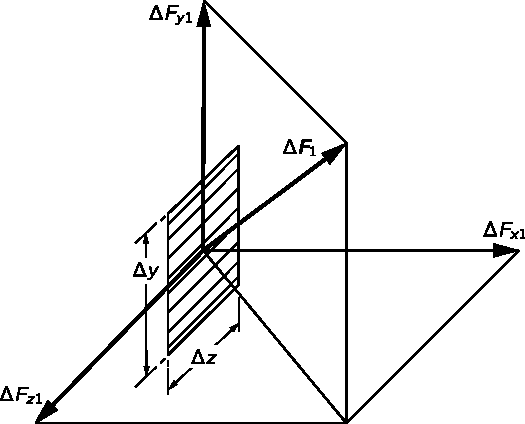
\includegraphics[width=0.8\linewidth]{fyz_fig0879.pdf}
      \caption{\(\Delta F_1\) působící na plošný element \(\Delta y\Delta z\) kolmý na osu \(x\) se
              rozkládá na tři složky \(\Delta F_{x1}\), \(\Delta F_{y1}\) a \(\Delta F_{z1}\)
              (\cite[s.~584]{Feynman02})}
      \label{fyz:fig0879}
    \end{figure}

    Jeden druh napětí už známe, a to statický tlak v kapalině. V tom případě je síla kolmá na
    povrchový element a je rovna tlaku vynásobenému povrchem. Pro pevné látky (jakož i pro
    pohybující se viskózní kapaliny) nemusí být síla kolmá na povrch, působí tu kromě tlaků
    (kladných nebo záporných) i \textbf{smykové síly}. (Smykovou silou rozumíme \emph{tangenciální}
    složku síly působící na povrch.) Všechny tři složky síly je třeba vzít v úvahu. Všimněme si, že
    bude-li mít náš řez rovinou jinou orientaci, budou síly jiné. K úplnému popisu vnitřního napětí
    potřebujeme tenzor.
    
    \emph{Tenzor napětí} definujeme takovýmto způsobem: Představme si nejdříve řez kolmý na osu
    \(x\) a rozložme sílu \(Δ\vec{F_1}\) působící v řezu na složky \(ΔF_{x1}\), \(ΔF_{y1}\),
    \(ΔF_{z1}\){ (obr. \ref{fyz:fig0879}). Podíl těchto sil a plošky \(\Delta y\Delta z\) označujeme
    \(S_{xx}\), \(S_{yx}\) a \(S_{zx}\). Například
    \begin{equation*}
      S_{yx}=\frac{\Delta F_{y1}}{\Delta y\,\Delta z}.
    \end{equation*}
    První index \(y\) se vztahuje ke směru silové složky a druhý index \(x\) ke směru, který má
    kolmice na plochu. Chceme-li, můžeme psát plochu \(\Delta y\Delta z\) jako \(\Delta a_x\), čímž
    myslíme plošný element kolmý na \(x\). Pak
    \begin{equation*}
      S_{yx}=\frac{\Delta F_{y1}}{\Delta a_x}.
    \end{equation*}

    \begin{figure}[ht!] %\ref{fyz:fig0880}
      \centering
      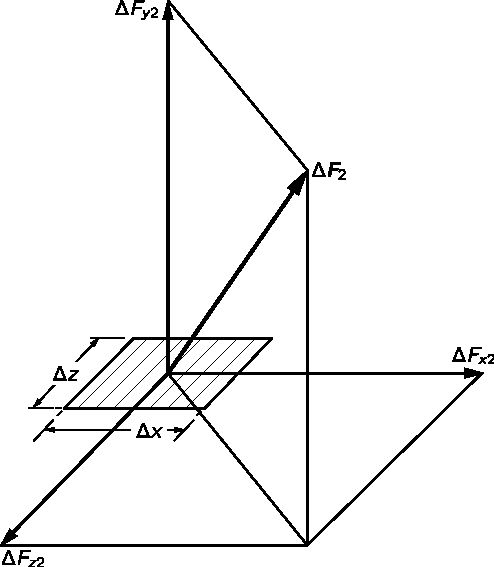
\includegraphics[width=0.8\linewidth]{fyz_fig0880.pdf}
      \caption{Síla působící na plošný element kolmý na \(y\) se rozkládá na tři navzájem kolmé
               složky (\cite[s.~584]{Feynman02})}
      \label{fyz:fig0880}
    \end{figure}

    Dále si představíme řez kolmý na osu \(y\). Na malou plošku \(\Delta x \Delta z\) působí síla
    \(Δ\vec{F_2}\). Opět rozložíme tuto sílu na tři složky tak, jak je to na obr. \ref{fyz:fig0880}.
    Z a definujeme tři složky napětí \(S_{xy}\), \(S_{yy}\), \(S_{zy}\) jako sílu působící na
    jednotkovou plochu ve třech směrech. Nakonec provedeme řez kolmo na \(z\) a definujeme tři
    složky \(S_{xz}\), \(S_{yz}\) a \(S_{zz}\). Máme tedy devět čísel:
    \begin{equation}\label{fyz:eq951}
      S_{ij}=
        \begin{bmatrix}
          S_{xx} & S_{xy} & S_{xz}  \\
          S_{yx} & S_{yy} & S_{yz}  \\
          S_{zx} & S_{zy} & S_{zz}  \\
        \end{bmatrix}.
    \end{equation}

    Nyní chceme ukázat, že těchto devět čísel stačí k úplnému popisu stavu vnitřního napětí a že
    \(S_{ij}\) je skutečně tenzorem. Předpokládejme, že chceme najít sílu působící na povrch pod
    nějakým libovolným úhlem. Můžeme ji určit z \(S_{ij}\)? Ano, můžeme, a to takovýmto způsobem:
    představme si malý, pevný hranol, jehož jedna stěna \(N\) je šikmá a ostatní dvě jsou rovnoběžné
    se souřadnicovými osami. Je-li stěna \(N\) rovnoběžná s osou \(z\), máme trojhranný útvar
    znázorněný na obr. \ref{fyz:fig0881}. (Je to trochu speciální případ, ale dostatečně ilustruje
    obecnou metodu.) Síly napětí působící na hranolek na obr. \ref{fyz:fig0881} jsou v rovnováze
    (přinejmenším v limitě nekonečně malých rozměrů), proto výsledná síla musí být rovna nule. Síly
    působící na stěny rovnoběžné se souřadnicovými osami zjistíme přímo z \(S_{ij}\). Jejich
    vektorový součet musí být roven síle působící na stěnu \(N\) takže tuto sílu umíme určit pomocí
    \(S_{ij}\).

    \begin{figure}[ht!] %\ref{fyz:fig0881}
      \centering
      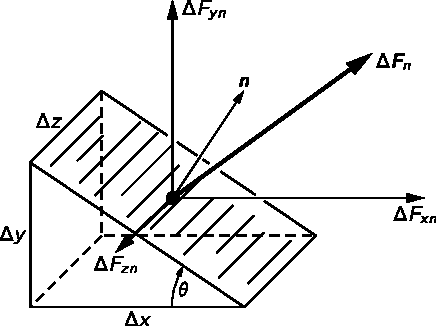
\includegraphics[width=0.8\linewidth]{fyz_fig0881.pdf}
      \caption{Síla\(\Delta F_n\) působící na plochu \(N\) (s jednotkovým vektorem \(\vec{n}\)) se
               rozkládá na tři složky (\cite[s.~585]{Feynman02})}
      \label{fyz:fig0881}
    \end{figure}

    Za našeho předpokladu, že \emph{plošné} síly působící na malý objem jsou v rovnováze,
    zanedbáváme všechny jiné \emph{objemové} síly, které by mohly být přítomny, například gravitaci
    nebo pseudosíly v případě, že naše souřadnicová soustava není inerciální soustavou. Všimněme si
    však, že takové objemové síly budou úměrné objemu hranolku, a tedy úměrné \(ΔxΔyΔz\), zatímco
    plošné síly jsou úměrné ploškám \(ΔxΔy\), \(ΔyΔz\) atd. Proto zvolíme-li si hranolek dostatečně
    malých rozměrů, budou objemové síly vždy zanedbatelné ve srovnání s plošnými silami.
    
    Nyní sečteme všechny síly působící na náš hranolek. Nejdříve vezměme složku \(x\), která je
    sumou pěti částí - po jedné z každé stěny. Je-li však \(Δz\) dostatečně malé, budou síly
    působící na trojúhelníkové stěny (kolmé na osu \(z\)) stejně velké a opačné, můžeme na ně tedy
    zapomenout. Složka \(x\) síly působící na spodní obdélník je
    \begin{equation*}
      \Delta F_{x2}=S_{xy}\,\Delta x\,\Delta z.
    \end{equation*}
    a \(x\)-ová složka síly působící na svislý obdélník je
    \begin{equation*}
      \Delta F_{x1}=S_{xx}\,\Delta y\,\Delta z.
    \end{equation*}
    Součet těchto dvou sil musí být roven \(x\)-ové složce síly působící na plochu \(N\) a směřující
    \emph{ven}. Nechť \(\vec{n}\) je jednotkový vektor kolmý na plochu \(N\) a \(\vec{F_n}\) nechť
    je síla působící na \(N\). Pak máme
    \begin{equation*}
      \Delta F_{xn}=S_{xx}\,\Delta y\,\Delta z+S_{xy}\,\Delta x\,\Delta z.
    \end{equation*}
    Složka \(S_{xn}\) napětí působícího na tuto plochu je rovna \(\Delta F_{xn}\) dělenému velikostí
    plochy \(\Delta z\sqrt{\Delta x^2+\Delta y^2}\), tj.
    \begin{equation*}
      S_{xn}=S_{xx}\,\frac{\Delta y}{\sqrt{\Delta x^2+\Delta y^2}}+
      S_{xy}\,\frac{\Delta x}{\sqrt{\Delta x^2+\Delta y^2}}.
    \end{equation*}
    Výraz \(\Delta x/\sqrt{\Delta x^2+\Delta y^2}\) je však kosinem úhlu \(\theta\) jenž svírají
    vektor \(\vec{n}\) a osa \(y\), jak to vidíme na obr. \ref{fyz:fig0881} - lze jej proto psát jako
    složkuy vektoru \(\vec{n}\), tj. jako \(n_y\). Podobně pro \(\Delta y/\sqrt{\Delta x^2+\Delta
    y^2}\) platí \(\sin\theta=n_x\). Můžeme psát
    \begin{equation*}
      S_{xn}=S_{xx}n_x+S_{xy}n_y.
    \end{equation*}
    Zobecníme-li to nyní na libovolný elementární povrch, dostaneme
    \begin{equation*}
      S_{xn}=S_{xx}n_x+S_{xy}n_y+S_{xz}n_z
    \end{equation*}
    nebo obecně
    \begin{equation}\label{fyz:eq952}
      S_{in}=\sum_jS_{ij}n_j.
    \end{equation} 
    Je tedy možné vyjádřit sílu působící na libovolnou elementární plochu pomocí koeficientů
    \(S_{ij}\), které tak úplně popisují vnitřní napětí v látce.

    \begin{figure}[ht!] %\ref{fyz:fig0882}
      \centering
      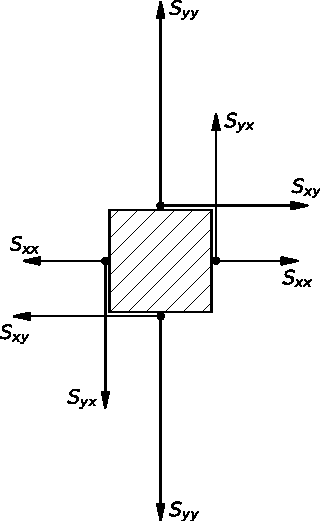
\includegraphics[width=0.7\linewidth]{fyz_fig0882.pdf}
      \caption{Složky sil \(x\) a \(y\) působících na čtyři stěny malé jednotkové krychle
               (\cite[s.~586]{Feynman02})}
      \label{fyz:fig0882}
    \end{figure}

    Rovnice \eqref{fyz:eq952} nám říká, že tenzor \(S_{ij}\) dává do vztahu sílu \(\vec{S_n}\) a
    jednotkový vektor \(\vec{n}\) právě tak, jako \(\alpha_{ij}\), dává do vztahu \(\vec{P}\) a
    \(\vec{E}\). Jelikož \(\vec{n}\) a \(\vec{S_n}\) jsou vektory, musí se složky \(S_{ij}\)
    transformovat při změně souřadnic jako tenzor. \(S_{ij}\) je tedy skutečně tenzorem.

    Jelikož \(S_{ij}\) je symetrickým tenzorem, může být popsán elipsoidem se třemi hlavními osami.
    Pro plochy kolmé na tyto osy jsou napětí obzvlášť jednoduchá - odpovídají tlaku nebo tahu
    kolmému na danou plochu. Podél těchto ploch nepůsobí žádné smykové síly. Pro \emph{libovolné}
    napětí můžeme vždy zvolit naše osy tak, aby byla smyková složka síly rovna nule. Je-li
    elipsoidem koule, působí v \emph{libovolném} směru jen kolmé složky. To odpovídá hydrostatickému
    tlaku (kladnému nebo zápornému). Pro hydrostatický tlak je tedy tenzor diagonální a všechny tři
    složky jsou navzájem rovny. Ve skutečnosti jsou rovny právě tlaku \(p\). Můžeme psát
    \begin{equation}\label{fyz:eq953}
      S_{ij}=p\delta_{ij}.
    \end{equation}

    Tenzor napětí, jakož i jeho elipsoid, se budou obecně měnit v dané látce od bodu k bodu.
    Chceme-li popsat daný kus látky, musíme udat hodnotu každé složky \(S_{ij}\) jako funkci polohy.
    Tenzor napětí je tedy \textbf{polem}. Poznali jsme už skalární pole, jako například teplotu
    \(T(x,y,z)\), v nichž je každému bodu v prostoru přiděleno jedno číslo, a vektorová pole jako
    \(\vec{E(x,y,z)}\), v nichž se každému bodu přiřazuje trojice čísel. Nyní máme tenzorové pole,
    kde je každému bodu prostoru přiřazeno devět čísel, nebo vlastně šest, protože \(S_{ij}\), je
    symetrický tenzor. Pro úplný popis vnitřních sil působících v libovolně deformované látce
    potřebujeme šest funkcí proměnných \(x, y, z\).
 
  \section{Tenzory vyššího řádu}\label{fyz:IIchapXXXIsecVII}
    
    Tenzor napětí \(S_{ij}\) popisuje \emph{vnitřní síly} v látce. Je-li látka elastická, je výhodné
    popisovat vnitřní \textbf{deformace} pomocí jiného tenzoru \(T_{ij}\), která se nazývá tenzor
    \emph{deformace}. Pro jednoduchý objekt, jako je například kovová tyč, umíme určit změnu délky
    \(ΔL\) podle \emph{Hookova zákona}, který říká, že prodloužení je přibližně úměrné síle:
    \begin{equation*}
      \Delta L=\gamma F.
    \end{equation*}
    
    Pro libovolné deformace pružného tuhého tělesa je vztah mezi deformací \(T_{ij}\) a napětím
    \(S_{ij}\) určen systémem lineárních rovnic 
    \begin{equation}\label{fyz:eq954}
      T_{ij}=\sum_{k,l}\gamma_{ijkl}S_{kl}.
    \end{equation}
    Také víme, že potenciální energie pružiny (nebo tyče) je rovna
    \begin{equation*}
      \dfrac{1}{2}F\,\Delta L=\dfrac{1}{2}\gamma F^2.
    \end{equation*}    
    Obecný výraz pro hustotu elastické energie pevného tělesa je
    \begin{equation}\label{fyz:eq955}
      U_{\text{elastic}}=\sum_{ijkl}\dfrac{1}{2}\gamma_{ijkl}S_{ij}S_{kl}.
    \end{equation}
    
    Úplný popis elastických vlastností krystalu je určen koeficienty \(\gamma_{ijkl}\). Tímto
    představujeme novou „obludu“ - \textbf{tenzor čtvrtého řádu}. Jelikož každý index může nabývat
    libovolnou ze tří hodnot \(x\), \(y\) nebo \(z\), dostáváme dohromady \(3^4 = 81\) koeficientů.
    Jenže ve skutečnosti je to jen 21 různých čísel. Zaprvé, jelikož tenzor \(S_{ij}\) je
    symetrický, obsahuje jen šest různých hodnot a v rovnici \eqref{fyz:eq955} potřebujeme jen 36
    \emph{různých} koeficientů. Zároveň však můžeme zaměnit \(S_{IJ}\) za \(S_{kl}\), aniž bychom
    změnili energii, proto \(\gamma_{ijkl}\) musí být symetrický při záměně \(ij\) za \(KL\). Tím se
    snižuje počet různých koeficientů na 21. Proto K popisu elastických vlastností krystalu s
    nejnižší možnou symetrií je třeba 21 elastických konstant! Tento počet je, samozřejmě, nižší pro
    krystaly s vyšší symetrií. Například krychlový krystal má jen tři pružné konstanty a izotropní
    látka má jen dvě.
    
    O správnosti předcházejícího tvrzení se můžeme přesvědčit. Jak mohou být složky tenzoru
    \(\gamma_{ijkl}\) nezávislé na směru os tak, jak to vyžadujeme pro izotropní látky? Odpověď je
    následující. Mohou být nezávislé \emph{jen} tehdy, když je lze vyjádřit pomocí tenzoru
    \(\delta_{ij}\). Existují dva možné výrazy \(\delta_{ij}\delta_{kl}\) a
    \(\delta_{ik}\delta_{jl}+\delta_{il}\delta_{jk}\) které mají požadovanou symetrii, proto
    \(\gamma_{ijkl}\) musí být jejich lineární kombinací. Proto pro izotropní látky platí
    \begin{equation*}
      \gamma_{ijkl}=a(\delta_{ij}\delta_{kl})+b(\delta_{ik}\delta_{jl}+\delta_{il}\delta_{jk}),
    \end{equation*}
    a potřebujeme dvě konstanty \(a\) a \(b\) k popisu elastických vlastností látky. Důkaz, že
    krychlový krystal potřebuje tři konstanty, přeskočíme.
    
    Jako poslední příklad, tentokrát na tenzor třetího řádu, uvádíme piezoelektrický efekt.
    Působením napětí se v krystalu vytváří elektrické pole úměrné napětí. Obecný zákon má tvar
    \begin{equation*}
      E_i=\sum_{j,k}P_{ijk}S_{jk},
    \end{equation*}
    kde \(E_i\) je elektrické pole a \(P_{ijk}\) jsou piezoelektrické koeficienty nebo
    piezoelektrický tenzor. Uměli bychom dokázat, že má-li krystal střed inverze (invariance při
    záměně \(x,y,z\to-x,-y,-z\) všechny piezoelektrické koeficienty jsou rovny nule?

  \section{Čtyřtenzor elektromagnetické energie a hybnosti}\label{fyz:IIchapXXXIsecVIII} 
    Všechny tenzory, které jsme v této kapitole dosud probírali, se vztahují k trojrozměrnému
    prostoru. Jsou definovány jako veličiny, které mají určité transformační vlastnosti při
    trojrozměrných rotacích. V kapitole \ref{fyz:IIchapXXVI} jsme měli možnost pracovat s tenzorem
    ve \emph{čtyřrozměrném relativistickém časoprostoru}, a to s tenzorem elektromagnetického pole
    \(F_{\mu\nu}\). Složky takového čtyřtenzoru se při Lorentzově transformaci souřadnic
    transformují určitým způsobem, který jsme odvodili. (Ačkoli jsme to tak nedělali, mohli jsme
    Lorentzovy transformace považovat za „rotace“ ve čtyřrozměrném „prostoru“, který se nazývá
    \emph{Minkowského prostor}. Pak by i analogie s tím, co nyní děláme, byla jasnější.)
    
    Jako náš poslední příklad zmíníme ještě jeden čtyřrozměrný tenzor z teorie relativity. Když jsme
    hovořili o tenzoru napětí, definovali jsme \(S_{ij}\) jako složky sil působících na jednotlivé
    plochy. Ale síla je rovna časové změně hybnosti. Proto místo výroku „\(S_{xy}\) je složkou \(x\)
    síly působící na jednotkovou plochu kolmou na \(y\)“ bychom stejně správně mohli říci
    „\(S_{xy}\) je rychlost změny toku složky \(x\) hybnosti jednotkovou plochou kolmou na \(y\).
    Jinými slovy, každá složka \(S_{ij}\) představuje i hustotu toku \(i\)-té složky hybnosti
    jednotkovou plochou kolmou na směr \(j\). Tyto čistě prostorové složky jsou však součástí
    „většího“ tenzoru \(S_{\mu\nu}\) ve čtyřech rozměrech (\(\mu\) a \(v= t, x,y,z\), který obsahuje
    navíc složky typu \(S_{xx}\), \(S_{xy}\), a \(S_{xz}\) atd. Nyní se pokusíme najít fyzikální
    význam těchto dodatečných složek.
    
    Víme, že prostorové složky představují hustotu toku hybnosti. Klíč k interpretaci časové složky
    nám poskytne jiný druh „toku“ - tok elektrického náboje. Rychlosti toku \emph{skalární}
    veličiny, náboje (jednotkovou plochou kolmou na tok), přiřazujeme prostorový vektor - vektor
    proudové hustoty \(\vec{j}\). Viděli jsme, že časová složka tohoto vektoru toku představuje
    hustotu toho, co teče. Například \(\vec{j}\) můžeme kombinovat s hustotou náboje \(\varrho\) a
    dostaneme čtyřvektor \(j_\mu=(\varrho,\vec{j})\) tj. index \(\mu\) v \(i_\mu\) nabývá hodnoty
    \(t\), \(x\), \(y\), \(z\), což postupně označuje hustotu, hustotu toku ve směru \(x\), hustotu
    toku ve směru \(y\) hustotu toku ve směru \(z\) skalárního náboje.
    
    Nyní, v analogii s naším tvrzením o časové složce toku skalární veličiny, bychom mohli očekávat,
    že vedle \(S_{xx}\), \(S_{xy}\), a \(S_{xz}\), které popisují tok \(x\)-ové složky hybnosti,
    existuje i časová složky \(S_{xt}\), která představuje hustotu toho, co teče, tj. \(S_{xt}\) by
    měla být hustotou \(x\)-ové složky hybnosti. Náš tenzor tak můžeme horizontálně rozšířit o
    složku \(t\). Dostaneme:
    \begin{itemize}[noitemsep]
      \item \(S_{xt}\ldots\) hustota \(x\)-ové složky hybnosti,
      \item \(S_{xx}\ldots\) hustota toku \(x\)-ové složky hybnosti ve směru \(x\),
      \item \(S_{xy}\ldots\) hustota toku \(x\)-ové složky hybnosti ve směru \(y\),
      \item \(S_{xz}\ldots\) hustota toku \(x\)-ové složky hybnosti ve směru \(z\).
    \end{itemize}
    Podobně pro \(y\)-ovou složku hybnosti máme tři složky hustoty toku \(S_{yx}\), \(S_{yy}\),
    \(S_{yz}\), k nimž přidáme čtvrtou složku
    
    \begin{center}
      \(S_{yt}\) = hustota \(y\)-ové složky hybnosti.
    \end{center}

    A samozřejmě, k \(S_{zz}\) bychom měli přidat
    \begin{center}
      \(S_{zt}\) = hustota \(z\)-ové složky hybnosti.
    \end{center}
    
    Ve čtyřech rozměrech existuje i složka \(t\) hybnosti, a to je, jak víme, energie. Proto by
    tenzor \(S_{ij}\) měl být rozšířen i vertikálně o složky \(S_{tx}\), \(S_{ty}\), a \(S_{tz}\)
    kde
    \begin{itemize}[noitemsep]
      \item \(S_{tx}\ldots\) hustota toku energie ve směru \(x\),
      \item \(S_{ty}\ldots\) hustota toku energie ve směru \(y\),
      \item \(S_{tz}\ldots\) hustota toku energie ve směru \(z\).
    \end{itemize}
    tj. \(S_{tx}\) je tok energie jednotkovou plochou kolmou k ose \(x\) na jednotku času atd.
    Nakonec, abychom zkompletovali náš tenzor, potřebujeme \(S_{tt}\) a to by měla být
    \textbf{hustota energie}. Náš trojrozměrný tenzor napětí \(S_{ij}\) jsme tak rozšířili na
    \textbf{čtyřrozměrný tenzor energie a hybnosti} \(S_{\mu\nu}\). Index \(\mu\) může nabývat čtyř
    hodnot \(t\), \(x\), \(y\), \(z\), které postupně označují hustotu, hustotu toku ve směru \(x\)
    hustotu toku ve směru \(y\) a hustotu toku ve směru \(z\). Podobně \(\nu\) nabývá čtyř hodnot
    \(t\), \(x\), \(y\), \(z\), které označují to, \emph{co} teče: energii, hybnost ve směru \(x\)
    hybnost ve směru \(y\) a hybnost ve směru \(z\).
    
    Jako příklad budeme tento tenzor uvažovat ne v látce, ale v nějaké oblasti volného prostoru, kde
    působí elektromagnetické pole. Víme, že hustota toku energie je určena \emph{Poyntingovým
    vektorem} \(\vec{S}=\epsilon_0c^2\vec{E}\times\vec{B}\). Z relativistického hlediska jsou složky
    \(x\), \(y\), \(z\) vektoru \(\vec{S}\) složkami \(S_{tx}\), \(S_{ty}\), a \(S_{tz}\) našeho
    čtyřrozměrného tenzoru energie a hybnosti. Symetrie tenzoru \(S_{ij}\) platí stejně i pro časové
    složky, proto je čtyřrozměrný tenzor \(S_{\mu\nu}\) symetrický
    \begin{equation}\label{fyz:eq956}
      S_{\mu\nu}=S_{\nu\mu}.
    \end{equation}
    Jinými slovy, složky \(S_{xt}\), \(S_{yt}\), \(S_{zt}\), které představují hustoty složek \(x\),
    \(y\) a \(z\) hybnosti, jsou zároveň složkami \(x\), \(y\) a \(z\) Poyntingova vektoru
    \(\vec{S}\), který představuje hustotu toku energie, jak jsme už ukázali v jedné z
    předcházejících kapitol.
    
    Zbývající složky elektromagnetického tenzoru energie a hybnosti \(S_{\mu\nu}\) lze také vyjádřit
    pomocí elektrického a magnetického pole \(\vec{E}\) a \(\vec{B}\). Musíme tedy připustit
    existenci napětí nebo, aby to neznělo tak záhadně, existenci toku hybnosti v elektromagnetickém
    poli. Mluvili jsme o tom v kapitole \ref{fyz:IIchapXXVII} v souvislosti s rovnicí
    \eqref{fyz:eq957}, ale tehdy jsme nešli do detailů.
    
    Chceme-li si vyzkoušet svou zručnost v zacházení s tenzory ve čtyřech rozměrech, je dobré
    vědět, jak \(S_{\mu\nu}\) vyjádřit pomocí polí:
    \begin{equation*}
      S_{\mu\nu}=-\varepsilon_0\biggl(
      \sum_\alpha F_{\mu\alpha}F_{\nu\alpha}-\dfrac{1}{4}\delta_{\mu\nu}
      \sum_{\alpha,\beta}F_{\beta\alpha}F_{\beta\alpha}
      \biggr),
    \end{equation*}
    kde sčítání přes \(\alpha\), \(\beta\) znamená sčítání přes \(t\), \(x\), \(y\), \(z\), ale (jak
    to bývá zvykem v teorii relativity) sumační znak \(\sum\) a symbol \(\delta\) mají speciální
    význam. Při sumaci se členy s \(x\), \(y\), \(z\) odčítají a \(δ_{tt}=+1\), zatímco \(δ_{xx} =
    δ_{yy} = δ_{zz}= −1\) a \(δ_{μ\nu}=0\) pro \(μ≠ν\) (\(c=1\)). Uměli bychom ověřit, že toto
    vyjádření vede k hustotě energie \(S_{tt}=(\varepsilon_0/2)\,(E^2+B^2)\) a k Poyntingovu vektoru
    \(\varepsilon_0\vec{E}\times\vec{B}\)? Uměli bychom ukázat, že v elektrostatickém poli, kde
    \(\vec{B}= 0\), mají hlavní osy napětí směr elektrického pole a že ve směru pole vzniká napětí
    \((\varepsilon_0/2)E^2\), zatímco ve směru kolmém na pole vzniká stejně velký \emph{tlak}?
%==== Kapitola Vnitřní geometrie krystalů ==========================================================
% !TeX spellcheck = cs_CZ
%{\tikzset{external/prefix={tikz/FYZII/}}
% \tikzset{external/figure name/.add={ch30_}{}}
%---------------------------------------------------------------------------------------------------
% file fey2ch30.tex
%---------------------------------------------------------------------------------------------------
%=========================== Kapitola Vnitřní geometrie krystalů ===================================
\setchaptertoc
\chapter{Vnitřní geometrie krystalů}\label{fyz:IIchapXXX}
  \section{Vnitřní geometrie krystalů}\label{fyz:IIchapXXXsecI}
    Studium základních zákonů elektřiny a magnetizmu jsme ukončili a nyní se budeme věnovat studiu 
    elektromagnetických vlastností látky. Začneme popisem pevných látek, tj. krystalů. Když se 
    atomy v látce příliš nepohybují, zůstávají seskupeny jeden u druhého v konfiguraci s nejnižší 
    možnou energií. Jestliže se atomy v jednom místě uspořádají tak, aby měly malou energii, je 
    pravděpodobné, že se na nějakém jiném místě uspořádají stejně. To je důvod, proč se v pevných 
    látkách opakují stejné konfigurace atomů.

    Jinými slovy, podmínky v krystalu jsou následující: Okolí každého atomu v krystalu je určitým 
    způsobem uspořádáno a podíváme-li se na atom stejného druhu na jiném, vzdálenějším místě, 
    zjistíte, že jeho okolí je přesně stejné. A vybereme-li si jiný atom, vzdálený o tutéž 
    vzdálenost, ještě dále, zjistíme, že podmínky jsou opět tytéž. Uspořádání se opakuje znovu a 
    znovu, samozřejmě, ve všech třech rozměrech.

    \begin{figure}[ht!]  %\ref{fyz:fig733}
      \centering
      \subcaptionbox{\label{fyz:fig733a}}{\luafigure[0.45]{fyz_fig733a.pdf}}
      \subcaptionbox{\label{fyz:fig733b}}{\luafigure[0.45]{fyz_fig733b.pdf}} 
      \caption{Opakující se vzorek ve dvou rozměrech 
               (\cite[s.~748]{Feynman02})}
      \label{fyz:fig733}
    \end{figure}
    
    Představme si, že máme navrhnout vzor tapety nebo látky, nebo nějaký jiný geometrický vzor na 
    rovinné ploše, přičemž se předpokládá, že navrhneme nějaký prvek, který se bude opakovat po tak 
    velké ploše, jak jen budeme chtít. Je to dvojrozměrná analogie problému, který se v krystalu 
    řeší ve třech rozměrech. Například obr. \ref{fyz:fig733a} představuje běžný druh tapetového 
    vzoru. Je tu jediný prvek, který se ve vzoru neustále opakuje. Geometrická charakteristika 
    tapetového dezénu, bereme-li v úvahu jen jeho periodické vlastnosti a nezajímáme se o geometrii 
    nebo uměleckou hodnotu samotného květu, je znázorněna na obr. \ref{fyz:fig733b}. Když začneme v 
    libovolném bodě, můžeme najít \emph{analogický} bod posunem o vzdálenost \(a\) ve směru šipky 
    \(1\). Analogický bod můžeme dostat i tehdy, posuneme-li se o vzdálenost \(b\) ve směru druhé 
    šipky. Existují, samozřejmě, i jiné směry. Můžeme například jít přímo z bodu \(\alpha\) do 
    \(\beta\)  dostat se do analogické polohy, jenže takový krok může být považován za postupnou 
    kombinaci kroků podél směru \(1\) a pak podél směru \(2\). Jedna ze základních vlastností vzoru 
    může být popsána dvěma nejkratšími kroky ke stejným sousedním polohám.
    
    \begin{figure}[ht!]
      \centering
      \subcaptionbox{\label{fyz:fig734}}{\luafigure[0.45]{fyz_fig734_1.jpg}}
      \subcaptionbox{\label{fyz:fig735}}{\luafigure[0.45]{fyz_fig735_1.jpg}}              \newline
      \subcaptionbox{\label{fyz:fig736}}{\luafigure[0.45]{fyz_fig736_1.jpg}}
      \caption{Přírodní krystaly: a) křemen b) chlorid sodný, c) slída
               (\cite[s.~545]{Feynman02})}
    \end{figure}

    Stejnými polohami myslíme, že kdybychom stáli v některé z těchto poloh a podívali bychom se 
    kolem, viděli bychom přesně totéž, jako kdybychom stáli v některé jiné poloze. To je základní 
    vlastnost krystalu. Jediný rozdíl jev tom, že krystal představuje trojrozměrné uspořádání místo 
    dvojrozměrného a, přirozeně, že místo květů představuje každý prvek mřížky určité uspořádání 
    atomů do nějaké konfigurace (například šest atomů vodíku a dva atomy uhlíku). Uspořádání atomů 
    v krystalu lze zjistit experimentálně pomocí rentgenové difrakce. 
    
    Vnitřní stavba krystalu se projevuje více způsoby. Za prvé, síla, která váže atomy navzájem, je 
    obvykle silnější v jednom směru než ve druhém. To znamená, že v krystalu existují plochy, podél 
    nichž je možné krystal snáze rozštěpit. Nazývají se \emph{štěpné} plochy. Rozbijeme-li krystal 
    čepelí nože, rozštěpí se většinou podél této plochy. Za druhé, vnitřní struktura je často 
    viditelná na povrchu díky způsobu, jakým krystal vznikl. Představme si, že se krystal vytváří 
    usazováním z roztoku. Atomy se v roztoku volně vznášejí až se nakonec, když najdou polohy s 
    nejnižší energií, usadí. (Je to, jako kdyby tapeta vznikala tak, že kvítky poletují sem a tam, 
    až se jeden náhodně dostane na určité místo a zůstane tam přilepen. Stejně je to s dalšími, až 
    se postupně vytváří celý vzor.) Chápeme, že v některých směrech roste krystal rychleji než v 
    jiných, a tím získává při růstu nějaký geometrický tvar. Díky tomuto jevu povrch mnoha krystalů 
    něco odráží z vlastností vnitřního uspořádání atomů,
    
    Tak například \ref{fyz:fig734} je znázorněn typický tvar krystalu křemene, jehož vnitřní 
    struktura je hexagonální. Všimneme-li si blíže celého krystalu, zjistíme, že zvenku to není 
    dokonalý šestiboký hranol, neboť stěny nejsou stejné dlouhé - ve skutečnosti bývají délkové 
    rozdíly dost velké. Ale z jednoho hlediska jde o velmi pravidelný šestiúhelník, \emph{úhly} 
    mezi stěnami mají přesně \SI{120}{\deg}. Je zřejmé, že velikosti té či oné hrany souvisí s 
    náhodnými procesy růstu, ale \emph{úhly} reprezentují vnitřní symetrii. Proto každý krystal 
    křemene má jiný tvar, ačkoliv úhly mezi jednotlivými stěnami jsou vždy tytéž. 
    
    Vnitřní symetrie krystalu chloridu sodného je také zřejmá z jeho vnějšího tvaru. Na obr. 
    \ref{fyz:fig735} je znázorněn typický tvar krystalu soli. Opět krystal není dokonalou krychlí, 
    ale stěny svírají přesně pravý úhel. 
    
    Komplikovanějším krystalem je slída, jejíž tvar je na obr. \ref{fyz:fig736}. Je to krystal s 
    velkým stupněm \emph{anizotropie}. Je to vidět i z toho, že je velmi těžké slídu v jednom směru 
    (na obrázku horizontálně), ale v jiném směru (vertikálně) ji lze štěpit velmi snadno. Tato 
    vlastnost se využívala k získávání velmi pevných tenkých vrstev. Slída a křemen jsou dva 
    příklady přírodních nerostů obsahujících oxid křemičitý. Dalším takovým příkladem je azbest, 
    který má tu vlastnost, že je snadno štěpitelný ve dvou směrech, ale ve třetím ne. Je vytvořen z 
    velmi silných \emph{lineárních} vláken. 
    
  \section{Chemické vazby v krystalech}\label{fyz:IIchapXXXsecII}
    Mechanické vlastnosti krystalů zřejmě závisejí na druhu chemických vazeb mezi atomy. Zarážející 
    rozdíly v pevnosti podél různých směrů ve slídě závisejí na druhu meziatomových vazeb v různých 
    směrech. V chemii jsme se učili o různých druzích chemických vazeb. Za prvé, jsou to 
    \emph{iontové vazby} o nichž jsme už hovořili v souvislosti s chloridem sodným. Zhruba řečeno, 
    atomy vodíku ztratí jeden elektron a stávají se kladnými ionty. Atomy chloru získají jeden 
    elektron a stávají se zápornými ionty. Kladné a záporné ionty jsou uspořádány do trojrozměrné 
    šachovnice a drží se navzájem elektrickými silami. 
    
    \begin{figure}[ht!] %\ref{fyz:fig737}
      \centering
      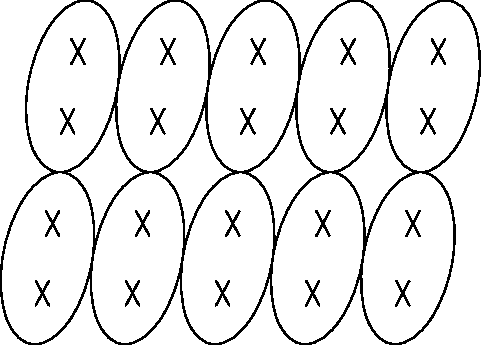
\includegraphics[width=0.5\linewidth]{fyz_fig737.pdf}
      \caption{Mřížka molekulového krystalu 
               (\cite[s.~546]{Feynman02})}
      \label{fyz:fig737}
    \end{figure}
    
    \emph{Kovalentní vazba}, v níž mají dva atomu společné elektronu, se vyskytuje častěji a 
    obvykle je velmi silná. 
    
    Například v diamantu jsou atomy uhlíku vázány kovalentně s nejbližšími sousedními atomy ve 
    všech čtyřech směrech, a proto je krystal skutečně velmi pevný. Kovalentní vazba je i mezi 
    křemíkem a kyslíkem v krystalu křemene, ale ve skutečnosti je to vazba jen částečně kovalentní, 
    Elektrony nejsou úplně společné, proto jsou atomy částečně nabité a krystal má v určitém smyslu 
    iontový charakter. Příroda není tak jednoduchá, jak se ji snažíme udělat. Ve skutečnosti 
    existují všechny možné stupně mezi kovalentní a iontovou vazbou.

    Krystal cukru má zase jiný druh vazby. Jsou v něm velké molekuly, jejichž atomy se silně drží 
    navzájem kovalentní vazbou, a proto má molekula tuhou strukturu. Ale jelikož silné vazby jsou 
    zcela nasyceny, zůstává jen relativně slabá přitažlivost mezi jednotlivými oddělenými 
    molekulami V takových \emph{molekulových} krystalech si molekuly zachovávají svou, řekněme, 
    individualitu a vnitřní uspořádání může být takové, jako vidíme na obr. \ref{fyz:fig737}. 
    Jelikož molekuly nejsou navzájem silně vázány, lze krystal snadno rozbít. Je to něco docela 
    jiného než diamant, který je skutečně jednou velkou molekulou, kterou nelze rozbít, aniž bychom 
    někde narušili kovalentní vazby. Parafín je další příklad molekulového krystalu.
    
    Extrémní příklad molekulového krystalu je pevný argon. Přitažlivost mezi atomy je v něm velmi 
    malá - každý atom je úplně saturovanou jedno atomovou molekulou. Při velmi nízkých teplotách je 
    však tepelný pohyb velmi slabý, proto nepatrné meziatomové síly mohou způsobit, že se atomy 
    uspořádají do pravidelného seskupení podobně jako kuličky při nejtěsnějším uspořádání.
    
    Kovy představují docela jinou třídu látek. Vazba je úplně jiná. Nevážou se sousední atomy, ale 
    vazba se vztahuje na celý krystal. Valenční atomy nepříslušejí jednomu atomu nebo dvojici 
    atomů, ale celému krystalu. Každý atom přispívá svým elektronem do společné „nádrže“ elektronů 
    a kladné ionty „přebývají v moři“ záporných elektronů. Elektronové moře představuje jakési 
    lepidlo, které drží ionty pohromadě.
    
    Jelikož v kovu neexistují žádné speciální vazby v určitém směru, není v jeho stavbě výrazná 
    závislost na směrech. Kovy však stále ještě patří mezi krystalické látky, protože jejich 
    celková energie je nejnižší tehdy, když jsou ionty atomů uspořádány v nějakém určitém seskupení 
    - ačkoliv energie tohoto preferovaného seskupení obvykle není o mnoho nižší než jiné možné 
    energie. V prvním přiblížení jsou atomy mnohých kovů uspořádány jako kuličky při nejtěsnějším 
    seskupení.
    
  \section{Růst krystalů}\label{fyz:IIchapXXXsecIII}
    Pokusme si představit, jak se přirozenou cestou vytvářely krystaly na Zemi. Zemská kůra 
    představuje směs atomů všech druhů. Ty se neustále mísí za pomoci sopečné činnosti, větru a 
    vody. Ale jakýmsi trikem se atomy křemíku postupně navzájem najdou a setkají se s atomy kyslíku 
    a vytvoří křemen. Jeden atom se vždy přidá k dalším a buduje se krystal. Směs přestává být 
    směsí. A kdesi nedaleko se setkávají atomy sodíku a chloru a vytvářejí krystal soli.
    
    Čím to je, že krystal, začne-li se jednou budovat, dovoluje jen určitému druhu atomů, aby se 
    připojoval? Je to tím, že celý systém usiluje o nejnižší možnou energii. Rostoucí krystal 
    přijme nový atom jen tehdy, když spolu s ním bude mít tak nízkou energii, jak je to jen možné. 
    Ale jak krystal ví, že umístěním atomu křemíku nebo kyslíku do určité polohy má zaručenu 
    nejnižší energii? Dělá to metodou pokusů a omylů. V tekutinách jsou všechny atomy v neustálém 
    pohybu. Každý atom naráží na svého souseda přibližně \num{e13}-krát za sekundu. Narazí-li na 
    správné místo v krystalu, kde je nízká energie, je menší pravděpodobnost, že se odrazí zpět. 
    Postupným zkoušením po dobu milionů let, při \num{e13} pokusech za sekundu, atomy postupně 
    budují krystal v místech, kde dosáhnou nejnižší energii. Nakonec tak narostou velké krystaly.
    
  \section{Krystalové mřížky}\label{fyz:IIchapXXXsecIV}
    Uspořádání atomů v krystalu - \textbf{krystalová mřížka} - může mít různé geometrické tvary. 
    Nejdříve popíšeme nejjednodušší mřížky, které jsou charakteristické pro většinu kovů a pro 
    inertní plyny v pevném skupenství. Jsou to krychlové mřížky, které se mohou vyskytovat ve dvou 
    tvarech: \emph{Prostorově centrovaná} (obr. \ref{fyz:fig738a}) a \emph{plošně centrovaná} 
    krychlová mřížka (obr. \ref{fyz:fig738b}). Nákresy samozřejmě znázorňují jen jednu krychli 
    mřížky. Musíme si představit, že vzor se opakuje do nekonečna ve třech rozměrech. Aby byl 
    obrázek názornější, jsou nakresleny jen „středy“ atomů. Ve skutečném krystalu jsou atomy téměř 
    jako koule, které jsou ve vzájemném kontaktu. Tmavé a světlé kuličky na obrázku mohou obecně 
    představovat buď různé, nebo stejné druhy atomů. Například železo má při nízkých teplotách 
    prostorově centrovanou krychlovou mřížku, ale při vysokých teplotách má plošně centrovanou 
    krychlovou mřížku. Fyzikální vlastnosti těchto dvou druhů krystalů jsou docela odlišné.
    
    \begin{figure}[ht!]   %\ref{fyz:fig738}
      \centering
      \subcaptionbox{\label{fyz:fig738a}}{\luafigure[0.45]{fyz_fig738a.pdf}}
      \subcaptionbox{\label{fyz:fig738b}}{\luafigure[0.45]{fyz_fig738b.pdf}} 
      \label{fyz:fig738}
      \caption{Elementární buňka krychlového krystalu a) prostorově centrovaná, b) plošně centrovaná
               (\cite[s.~547]{Feynman02})}
    \end{figure}
    
    Jak takové druhy krystalů vznikají? Představme si, že máme za úkol uspořádat sférické atomy 
    navzájem tak těsně, jak je to je m možné. Jeden způsob by byl udělat první vrstvu 
    šestiúhelníkového uspořádání, jak je znázorněno na obr. \ref{fyz:fig739a}. Pak můžeme vybudovat 
    druhou vrstvu podobně jako první, ale horizontálně posunutou (obr.\ref{fyz:fig739b}). Dále 
    můžete uložit třetí vrstvu. Ale pozor! Existují dva různé způsoby, jak umístit třetí vrstvu. 
    Začneme-li vytvářet třetí vrstvu tak, že umístíme atom do polohy \(A\) (obr. 
    \ref{fyz:fig739b}), bude každý atom v třetí vrstvě přímo nad atomem nejspodnější vrstvy. Když 
    však začneme třetí vrstvu vytvářet tak, že uložíme atom do polohy \(B\), budou atomy ve třetí 
    vrstvě mít svůj střed přesně nad bodem, který je středem trojúhelníka vytvořeného třemi atomy 
    spodní vrstvy. Každé jiné počáteční umístění je ekvivalentní buď s \(A\), nebo s \(B\), takže 
    jsou jen dva způsoby umístění třetí vrstvy.
    
    \begin{figure}[ht!]    %\ref{fyz:fig739}
      \centering
      \subcaptionbox{\label{fyz:fig739a}}{\luafigure[0.45]{fyz_fig739a.pdf}}
      \subcaptionbox{\label{fyz:fig739b}}{\luafigure[0.45]{fyz_fig739b.pdf}} 
      \label{fyz:fig739}
      \caption{Budování těsně uspořádané šestiúhleníkové mřížky
               (\cite[s.~548]{Feynman02})}
    \end{figure}

    Má-li třetí vrstva atom v bodě \(B\), je to plošně centrovaná krychlová mřížka - ale viděná pod 
    určitým úhlem. Vypadá to divně, že jsme začali šestiúhelníky a skončili jsme krychlemi. 
    Všimněme si však, že díváme-li se na krychli z jednoho vrcholu, vidíme šestiúhelníkové obrysy. 
    Například obr. \ref{fyz:fig740} by mohl představovat rovinný šestiúhelník nebo krychli viděnou 
    z perspektivy.
    
    \begin{figure}[ht!] %\ref{fyz:fig740}
      \centering
      \includegraphics[width=0.4\linewidth]{fyz_fig740.pdf}
      \caption{Je toto šestiúhelník nebo krychle při pohledu z jejího vrcholu?
               (\cite[s.~548]{Feynman02})}
      \label{fyz:fig740}
    \end{figure}
    
    Doplníme-li třetí vrstvu na obr. \ref{fyz:fig739b} tak, že začneme s atomem v \(A\), 
    nedostaneme krychlovou strukturu, ale místo toho má mřížka jen šesterečnou symetrii. Je zřejmé, 
    že obě možnosti, které jsme popsali, představují stejně těsné uspořádání.
    
    Některé kovy, například měď nebo stříbro, si vybírají první alternativu-plošně centrovanou 
    krychli. Jiné, například berylium a hořčík, volí jiné alternativy - vytvářejí šesterečné 
    krystaly. Je zřejmé, že to, jaký krystal se vytvoří, nezávisí jen na uspořádání malých kuliček, 
    ale musí to být částečně určeno i jinými faktory. Konkrétně je to malá úhlová závislost 
    meziatomových sil (nebo v případě kovů závislost na energii elektronové „nádrže“). Tohle 
    všechno se dozvíme na přednáškách z chemie.
    
  \section{Symetrie ve dvou rozměrech}\label{fyz:IIchapXXXsecV}
    Nyní bychom chtěli pohovořit o některých vlastnostech krystalů z hlediska jejich vnitřních 
    symetrií. Hlavním rysem krystalů je ta vlastnost, že když se přemístíme o jednu mřížkovou 
    jednotku od jednoho atomu k příslušnému dalšímu, budeme opět v témže prostředí. To je základní 
    předpoklad. Ale kdybychom byli atomem, byl by tu ještě jiný druh změny, která by nás dostala 
    opět do téhož prostředí, tj. jiná možná symetrie. Na obr. \ref{fyz:fig741a} je znázorněn další 
    možný „tapetový“ vzor. Předpokládejme, že porovnáme okolí bodů \(A\) a \(B\). Na první pohled 
    se nám může zdát, že jsou stejná - ale ne docela. Body \(C\) a \(D\) jsou ekvivalentní s bodem 
    \(A\), ale okolí bodu \(B\) je jako okolí bodu \(A\) jen tehdy, převrátíme-li jej, tj. v 
    zrcadlovém obrazu.

    \begin{figure}[ht!]    %\ref{fyz:fig741}
      \centering
      \subcaptionbox{\label{fyz:fig741a}}{\luafigure[0.95]{fyz_fig741a.pdf}}               \newline
      \subcaptionbox{\label{fyz:fig741b}}{\luafigure[0.95]{fyz_fig741b.pdf}} 
      \caption{Vzory s vyšší symetrií (\cite[s.~549]{Feynman02})}
      \label{fyz:fig741}
    \end{figure}

    V tomto vzoru jsou další druhy ekvivalentních bodů. Například body \(E\) a \(F\) mají stejné 
    okolí až na to, že jsou vzájemně otočeny o \SI{90}{\degree}. Rotace o úhel \SI{90}{\degree} 
    (nebo jeho libovolný násobek) kolem vrcholů, jako je \(A\), vede všude opět k témuž vzoru. 
    Krystal s takovouto strukturou je navenek pravoúhlý, ale uvnitř je komplikovanější než 
    jednoduchá krychle. Nyní, když jsme popsali některé speciální případy, pokusíme se přijít na 
    všechny možné symetrie, které může krystal mít. Nejdříve uvažujme, co se stane v rovině. 
    Rovinná mřížka může být definována dvěma \emph{základními} vektory, které mají počátek v jednom 
    bodě mřížky a koncové body ve dvou \emph{nejbližších} ekvivalentních bodech. Dva vektory 
    \(\bm{1}\) a \(\bm{2}\) jsou základními vektory mřížky na obr. \ref{fyz:fig733}. Dva vektory 
    \(\bm{a}\) a \(\bm{b}\) na obr. \ref{fyz:fig741a} jsou základními vektory znázorněného vzoru. 
    Mohli bychom, samozřejmě, vybrat \(\bm{-a}\) místo \(\bm{b}\) nebo \(\bm{-b}\) místo 
    \(\bm{a}\). Jelikož \(\bm{a}\) a \(\bm{b}\) mají stejnou velikost a jsou na sebe kolmé, přejde 
    při rotaci o \SI{90}{\degree} \(\bm{a}\) do \(\bm{b}\) a \(\bm{b}\) do \(\bm{-a}\), což nám 
    dává opět tutéž mřížku. Vidíme, že existují mřížky, které mají „čtyřstrannou“ symetrii. A před 
    tím jsme popsali těsné uspořádání založené na šestiúhelnících, které by mohlo mít 
    „šestistrannou“ symetrii. Seskupení kružnic na obr. \ref{fyz:fig739a} se při rotaci o 
    \SI{60}{\degree} kolem středu libovolné kružnice zobrazuje opět tentýž vzor. Jaké jiné druhy 
    rotační symetrie ještě existují? Můžeme mít například pětinásobné nebo osminásobné rotační 
    symetrie? Lze snadno vidět, že tyto jsou vyloučeny.\emph{ Jedinou symetrií, založenou na útvaru 
    s více než čtyřmi stranami, je šestistranná symetrie}. Nejdříve ukážeme, že symetrie s více než 
    šesti stranami je vyloučena. Zkusme si představit mřížku se dvěma stejně velkými základními 
    vektory, které svírají úhel menší než \SI{60}{\degree} (obr. \ref{fyz:fig742a}). Předpokládáme, 
    tedy, že body \(B\) a \(C\) jsou ekvivalentní s bodem \(A\) a že \(\bm{a}\) a \(\bm{b}\) jsou 
    dva nejkratší vektory od \(A\) k jeho ekvivalentním sousedům. To je však zřejmě nesprávné, 
    neboť vzdálenost mezi body \(B\) a \(C\) je menší než vzdálenost libovolného z nich od \(A\). 
    Musí tu být nějaký soused \(D\), který je ekvivalentní s \(A\) a je k němu blíže než \(B\) nebo 
    \(C\). Měli bychom zvolit \(\bm{b'}\) za jeden z našich základních vektorů. Proto úhel mezi 
    dvěma základními vektory musí být \SI{60}{\degree} nebo více. Osmiúhelníková symetrie není 
    možná.

    A co takhle pětinásobná symetrie? Předpokládáme-li, že základní vektory \(\bm{a}\) a \(\bm{b}\) 
    mají stejné délky a svírají úhel \(2\pi /5 = \SI{72}{\degree}\) (obr. \ref{fyz:fig742b}), měl 
    by existovat ekvivalentní mřížkový bod \(D\) odkloněný o \SI{72}{\degree} od \(C\). Ale vektor 
    \(\bm{b'}\) směřující od \(E\) do \(D\) je menší než \(\bm{b}\), proto \(\bm{b}\) není 
    základním vektorem. Pětinásobná symetrie nemůže existovat. Jediné možnosti, které nás 
    nepřivedou do těchto obtíží jsou \(\vartheta = \SI{60}{\degree}; \SI{90}{\degree}\) nebo 
    \SI{120}{\degree}. Nula nebo \SI{180}{\degree} jsou také zřejmě možné. Náš výsledek lze 
    zformulovat i tak, že vzor může zůstávat nezměněn při rotaci o celých \SI{360}{\degree} (vůbec 
    žádná změna), o jednu polovinu, jednu třetinu, jednu čtvrtinu nebo jednu šestinu celé otáčky. A 
    to jsou všechny možné rotační symetrie v rovině - celkem pět. Je-li \(\vartheta = 2\pi/n\), 
    mluvíme o \(n\)-násobné symetrii. Říkáme, že vzor s \(n\) rovným \(4\) nebo \(6\) má vyšší 
    symetrii než vzor s \(n\) rovným \(1\) nebo \(2\). 

    \begin{figure}[ht!]    %\ref{fyz:fig742}
      \centering
      \subcaptionbox{\label{fyz:fig742a}}{\luafigure[0.95]{fyz_fig742a.pdf}}               \newline
      \subcaptionbox{\label{fyz:fig742b}}{\luafigure[0.95]{fyz_fig742b.pdf}} 
      \caption{a) Rotační symetrie vyšší než šestinásobné nejsou možné. b) Pětinásobná symetrie 
               není možná.
               (\cite[s.~550]{Feynman02})}
      \label{fyz:fig742}
    \end{figure}

    Vraťme se k obr. \ref{fyz:fig741a}. Vidíme, že vzor má čtyřnásobnou rotační symetrii. Na obr. 
    \ref{fyz:fig741b} jsme nakreslili jiný vzor, který má tytéž vlastnosti symetrie jako obr. 
    \ref{fyz:fig741a}. Malé značky podobné čárkám jsou asymetrické objekty, které nám slouží k 
    určení symetrie vzoru uvnitř každého čtverečku. Všimněme si, že čárky v sousedních čtvercích 
    jsou převrácené, takže základní buňka je větší než jeden čtvereček. Kdyby nebyly čárky, měl by 
    vzor také čtyřnásobnou symetrii, ale základní buňka by byla menší. Vzor na obr. 
    \ref{fyz:fig741} má ještě další druhy symetrie. Například při zrcadlovém zobrazení vzhledem k 
    přerušovaným osám \(\bm{R} \rightarrow \bm{-R}\) dostaneme tentýž vzor. 

    A ještě je tu jeden druh symetrie pro vzor na obr. \ref{fyz:fig741}. Provedeme-li zrcadlový 
    obraz vzhledem k ose \(Y-Y\) \emph{plus} posun o jeden čtvereček doprava (nebo doleva), 
    dostaneme opět původní vzor. Čára \(Y-Y\) se nazývá \textbf{skluzná čára}.

    To jsou všechny možné symetrie pro dva rozměry. V prostoru existuje ještě jedna operace 
    symetrie, jíž v \emph{dvojrozměrném} případě odpovídá rotace o \SI{180}{\degree}, ale ve třech 
    rozměrech je to zcela odlišná operace. Je to \emph{inverze}. Inverzí rozumíme přemístění bodu, 
    jehož polohový vektor je \(\bm{R}\), do bodu \(\bm{-R}\) (obr. \ref{fyz:fig743b}). 

    \begin{figure}[ht!]   %\ref{fyz:fig743}
      \centering
      \subcaptionbox{\label{fyz:fig743a}}{\luafigure[0.45]{fyz_fig743a.pdf}}
      \subcaptionbox{\label{fyz:fig743b}}{\luafigure[0.45]{fyz_fig743b.pdf}}              \newline
      \subcaptionbox{\label{fyz:fig743c}}{\luafigure[0.45]{fyz_fig743c.pdf}}
      \subcaptionbox{\label{fyz:fig743d}}{\luafigure[0.45]{fyz_fig743d.pdf}} 
      \caption{Symetrie vzhledem k inverzi. Vzor b) zůstává nezměněn při \(\bm{R} \rightarrow 
               \bm{-R}\), ale vzor a) se mění. Trojrozměrný vzor d) je při inverzi symetrický, ale 
               c) není
               (\cite[s.~551]{Feynman02})}
      \label{fyz:fig743}
    \end{figure}

    Při inverzi vzoru na obr. \ref{fyz:fig743a} dostáváme nový vzor, ale při inverzi vzoru (obr. 
    \ref{fyz:fig743b}) se reprodukuje tentýž vzor. Pro dvojrozměrné vzory (jak vidíme na obrázku 
    \ref{fyz:fig743b}) je inverze vzoru vzhledem k bodu \(A\) ekvivalentní s rotací o 
    \SI{180}{\degree} kolem téhož bodu. Předpokládejme, že bychom vzor na obr. \ref{fyz:fig743b} 
    předělali na trojrozměrný tak, že bychom všechny malé znaky \num{6} a \num{9} doplnili šipkou 
    směřující ven z obrázku. Po inverzi v třech rozměrech by všechny šipky přešly na opačné, takže 
    by se vzor nereprodukoval. Označíme-li počátky šipek tečkami a konce křížky, můžeme sestavit 
    trojrozměrný vzor, jako je na obr. \ref{fyz:fig743c}, který není symetrický vzhledem k inverzi. 
    Můžeme také vytvořit vzor znázorněný na obr. \ref{fyz:fig743d}, který má takovou symetrii. 
    Všimněme si, že trojrozměrnou inverzi nelze nahradit nějakou kombinací rotací.

    Charakterizujeme-li symetrii vzoru - nebo mřížky - týmiž druhy operací symetrie, které jsme 
    popsali, lze ukázat, že ve dvojrozměrném případě může existovat \num{17} různých vzorů. Na obr. 
    \ref{fyz:fig733} jsme nakreslili vzor, který patří k vzorům s nejnižší symetrií, a na obr. 
    \ref{fyz:fig741} je ukázka vzoru s vyšší symetrií. S vymýšlením všech sedmnácti možných vzorů 
    si můžeme pohrát sami.
    
    Je zajímavé, jak málo vzorů ze všech \num{17} možných se používá při navrhování tapet a 
    textilních vzorů. Všude se setkáváme jen s týmiž třemi nebo čtyřmi základními vzory. Je to 
    nedostatek fantazie návrhářů, nebo je to proto, že ostatní vzory nelahodí oku?
    
  \section{Symetrie ve třech rozměrech}\label{fyz:IIchapXXXsecVI}
    Dosud jsme hovořili jen o dvojrozměrných vzorech. To, co nás však ve skutečnosti zajímá, je 
    uspořádání atomů ve třech rozměrech. Z prvé je zřejmé, že trojrozměrný krystal bude mít tři 
    základní vektory. Kdybychom se zeptali na možné operace symetrie ve třech rozměrech, zjistili 
    bychom, že existuje \num{230} různých možných symetrií. Z jistých důvodů rozdělujeme těchto 
    \num{230} typů na sedm tříd, které jsou znázorněny na obr. \ref{fyz:fig744}. Mřížka s nejnižší 
    symetrií se nazývá \textbf{trojklonná} Základní buňkou je \emph{rovnoběžnostěn}. Základní 
    vektory mají nestejné délky a žádné dva z úhlů, které navzájem svírají, nejsou stejné. Tato 
    mřížka nemá rotační symetrii ani symetrii odrazu. Dvě možné symetrie tu však přece jen jsou - 
    základní buňka je, nebo není změněna při inverzi vzhledem k jednomu vrcholu. (Inverzí v 
    trojrozměrném případě rozumíme záměnu vektoru posunutí \(\bm{R}\) na \(\bm{-R}\), jinými slovy 
    záměnu \((x, y, z)\) za \((-x, -y, -z)\).) Trojklonná mřížka má tedy jen dvě možné symetrie s 
    výjimkou případů, kdy základní vektory splňují určité speciální vztahy. Například jsou-li 
    všechny vektory stejné a svírají stejné úhly, dostáváme \textbf{klencovou} mřížku znázorněnou 
    na obrázku. Znázorněná buňka může mít ještě dodatečnou symetrii - může zůstat nezměněna při 
    rotaci kolem nejdelší, tělesové úhlopříčky.
    

    \begin{figure}[ht!]   %\ref{fyz:fig744}
      \centering
      \subcaptionbox{\label{fyz:fig744a}}{\luafigure[0.45]{fyz_fig744a.pdf}}
      \subcaptionbox{\label{fyz:fig744b}}{\luafigure[0.45]{fyz_fig744b.pdf}}              \newline
      \subcaptionbox{\label{fyz:fig744c}}{\luafigure[0.45]{fyz_fig744c.pdf}}
      \subcaptionbox{\label{fyz:fig744d}}{\luafigure[0.45]{fyz_fig744d.pdf}}              \newline
      \subcaptionbox{\label{fyz:fig744e}}{\luafigure[0.45]{fyz_fig744e.pdf}}
      \subcaptionbox{\label{fyz:fig744f}}{\luafigure[0.45]{fyz_fig744f.pdf}}              \newline
      \subcaptionbox{\label{fyz:fig744g}}{\luafigure[0.45]{fyz_fig744g.pdf}}
      \caption{Sedm tříd krystalických mřížek (\cite[s.~552]{Feynman02})}
      \label{fyz:fig744}
    \end{figure}
    
    Je-li jeden ze základních vektorů, například \(\bm{c}\), kolmý na ostatní dva vektory, 
    dostáváme základní \textbf{jednoklonnou} buňku. Novou možnou symetrií je rotace o 
    \SI{180}{\degree} kolem \(\bm{c}\). Speciálním případem je \textbf{šesterečná} buňka, v níž 
    jsou vektory \(\bm{a}\) a \(\bm{b}\) stejné a svírají úhel \SI{60}{\degree}, takže při rotaci o 
    \SI{60}{\degree}, \SI{120}{\degree} nebo \SI{180}{\degree} kolem vektoru \(\bm{c}\) dostáváme 
    tutéž mřížku (pro určité vnitřní symetrie).
    
    Jsou-li všechny tři základní vektory navzájem kolmé, ale mají různou délku, dostáváme 
    \textbf{kosočtverečnou} buňku. Buňka je symetrická při rotacích o \SI{180}{\degree} kolem tří 
    os. Symetrie vyššího řádu má \textbf{čtverečná} buňka, která má všechny úhly pravé a dva její 
    základní vektory mají stejnou délku. Nakonec je tu \textbf{krychlová} mřížka, která je nejvíce 
    symetrická ze všech.
    
    Smyslem všech těchto úvah o symetriích je to, že vnitřní symetrie krystalů se projevují, někdy 
    jen nenápadným způsobem, v makroskopických fyzikálních vlastnostech krystalu. Obecně je 
    například elektrická polarizovatelnost krystalu charakterizována tenzorem. Vyjádříme-li tento 
    tenzor pomocí elipsoidu polarizace, lze předpokládat, že tento elipsoid bude odrážet některé 
    vlastnosti symetrie krystalu. Například krychlový krystal je symetrický vzhledem k rotacím o 
    \SI{90}{\degree} kolem libovolné ze tří kolmých os. Je zřejmé, že jediný elipsoid s touto 
    vlastností je \emph{koule}. \emph{Krychlový krystal musí být izotropním dielektrikem}.
    
    Na druhé straně čtverečný krystal má čtyřnásobnou rotační symetrii. Jeho elipsoid musí mít dvě 
    z hlavních os stejné a třetí musí být rovnoběžná s osou krystalu. Podobně kosočtverečný 
    krystal, protože má dvojnásobnou rotační symetrii vzhledem ke třem navzájem kolmým osám, musí 
    mít osy totožné s osami elipsoidu polarizace. Podobně jedna z os jednoklonného krystalu musí 
    být rovnoběžná s jednou z hlavních os elipsoidu, ale o jeho dalších osách nemůžeme nic říci. 
    Protože trojklonný krystal nemá žádnou rotační symetrii, může být jeho elipsoid orientován 
    libovolně.
    
    Jak vidíme, mohli bychom si do nekonečna hrát s výčtem různých symetrií a určováním jejich 
    vztahu k různým fyzikálním tenzorům. Uvažovali jsme jen tenzor polarizovatelnosti, ale i s 
    jinými tenzory (například tenzorem pružnosti) je to komplikovanější. Existuje matematický obor 
    nazývaný teorie grup, který se těmito otázkami zabývá, ale obvykle se lze dopracovat k výsledku 
    jen na základě zdravého rozumu.
    
  \section{Pevnost kovů}\label{fyz:IIchapXXXsecVII}
    Řekli jsme si, že kovy mají obvykle krychlovou krystalickou strukturu. Nyní budeme hovořit o 
    jejich mechanických vlastnostech, které závisejí na této struktuře, Kovy jsou obecně velmi 
    „měkké“, neboť lze snadno posouvat jednu vrstvu krystalu vzhledem k druhé. Možná si řeknete: 
    „Vždyť je to nesmysl, kovy jsou přece pevné!“ Není to tak. \emph{Jednotlivé krystaly} kovu 
    můžeme snadno deformovat.
    
    \begin{figure}[ht!]    %\ref{fyz:fig745}
      \centering
      \subcaptionbox{\label{fyz:fig745a}}{\luafigure[0.8]{fyz_fig745a.pdf}}               \newline
      \subcaptionbox{\label{fyz:fig745b}}{\luafigure[0.8]{fyz_fig745b.pdf}} 
      \caption{Skluz krystalových rovin (\cite[s.~552]{Feynman02})}
      \label{fyz:fig745}
    \end{figure}
    
    Podívejme se na dvě vrstvy krystalu, na které působí smyková síly (obr. \ref{fyz:fig745a}). Na 
    první pohled se může zdát, že celá vrstva bude odolávat působení, dokud nebude síla dostatečně 
    velká na to, aby pohnula celou vrstvou „přes hrboly“, takže ta se posune o jedno místo doleva. 
    Ačkoli posun se vztahuje na celou rovinu, neprobíhá to tímto způsobem. (Kdyby to tak bylo, 
    vyšlo by vám, že kov má být mnohem pevnější, než ve skutečnosti je..) Spíše je to tak, jakoby 
    se atomy přemisťovaly jeden po druhém. Nejdříve poskočí atom, který je úplně nalevo, potom 
    další atd., jak je znázorněno na obr. \ref{fyz:fig745b}. Celkový efekt je takový, že prázdné 
    místo mezi dvěma atomy putuje rychle směrem doprava, až se nakonec celá vrstva přemístí o jednu 
    meziatomovou vzdálenost. Posun probíhá tímto způsobem proto, že se spotřebuje méně energie při 
    přesunutí jednoho atomu přes hrbol než při přesunu celé řady. Jakmile je síla dostatečně velká, 
    může proces začít a zbytek už postupuje velmi rychle.
    
    
    \begin{figure}[ht!] %\ref{fyz:fig746}
      \centering
      \includegraphics[width=0.7\linewidth]{fyz_fig746.jpg}
      \caption{Fotografie malého krystalu mědi po natažení (S dovolením S. S. Brennera, vědeckého 
               pracovníka Ocelářského výzkumného centra, Monroeville, Pensylvánie, USA.)
               (\cite[s.~552]{Feynman02})}
      \label{fyz:fig746}
    \end{figure}
    
    Ukazuje se, že ve skutečném krystalu probíhá posouvání opakovaně v jedné rovině, pak se zastaví 
    a začne v nějaké jiné rovině. Detailní zdůvodnění, proč proces začne a proč končí, zůstává 
    záhadou. Je vlastně velmi divné, že oblasti, v nichž posun postupně probíhá, bývají od sebe 
    přibližně stejně vzdáleny. Na obr. \ref{fyz:fig746} je fotografie malého tenkého krystalu mědi, 
    který byl „natahován“. Můžeme rozeznat různé roviny, v nichž nastalo posunutí.
    
    O náhlém posunu jednotlivých rovin krystalu se můžeme přímo přesvědčit. Vezmeme-li si kousek 
    tenkého drátku, který obsahuje velké krystaly, a napneme jej v blízkosti ucha, můžeme slyšet 
    „tikot“ provázející postupné zapadání rovin do svých nových poloh. 
    
    Problém „chybějícího“ atomu v řadě je o něco složitější, než se zdá z obr. \ref{fyz:fig745}. 
    Máme-li víc vrstev, vznikne podobná situace jako na obr. \ref{fyz:fig747}. 
    
    \begin{figure}[ht!] %\ref{fyz:fig747}
      \centering
      \includegraphics[width=0.7\linewidth]{fyz_fig747.pdf}
      \caption{Dislokace v krystalu
               (\cite[s.~554]{Feynman02})}
      \label{fyz:fig747}
    \end{figure}

    Taková nedokonalost v krystalu se nazývá \textbf{dislokace}. Předpokládá se, že dislokace jsou 
    buď přítomny v krystalu už při jeho formování, nebo se vytvoří u nějaké trhliny nebo zářezu na 
    povrchu. Když už jednou vzniknou, mohou se v krystalu poměrně volně pohybovat. Při pohybu 
    takovýchto dislokací vznikají větší deformace.
    
    Dislokace se mohou volně pohybovat, to znamená, že k tomu stačí malá dodatečná energie za 
    předpokladu, že zbytek krystalu je dokonalou mřížkou. Ale mohou se „zaseknout“, když se setkají 
    s nějakým jiným druhem defektu v krystalu. Je-li třeba velké energie k tomu, aby se dislokace 
    přes defekt dostaly, zastaví se. To je právě mechanizmus, který je příčinou pevnosti 
    nedokonalých kovových krystalů. Čisté krystaly železa jsou docela měkké, ale malá koncentrace 
    atomů příměsi může vyvolat tolik poruch, že dislokace budou efektivně znehybněny. Jak víme, 
    ocel, která je převážně železem, je velmi tvrdá. Při výrobě oceli se malé množství uhlíku 
    rozpustí v roztaveném železe. Při rychlém ochlazení vytvářejí zrníčka uhlíku v mřížce množství 
    mikroskopických poruch. Dislokace se už nemohou volně pohybovat a kov se stane pevným.
    
    \begin{figure}[ht!] %\ref{fyz:fig748}
      \centering
      \includegraphics[width=0.7\linewidth]{fyz_fig748.pdf}
      \caption{Dislokace v torzi (Z knihy Ch. Kittel: Úvod do fyziky pevných látek, v českém 
               překladu vyšlo v nakladatelství Academia, Praha 1985.)
               (\cite[s.~554]{Feynman02})}
      \label{fyz:fig748}
    \end{figure}
    
    Čistá měď je velmi měkká, ale může ji udělat tvrdší tím, že ji ohýbáme, nebo vyklepeme 
    kladivem. V tomto případě se vytváří mnoho nových dislokací různých druhů, které navzájem 
    interferují, a tak omezují svou pohyblivost. Vezměme kousek měkké mědi a snadno jej obtočíme 
    někomu kolem zápěstí jako náramek. Přitom se měď zpevní a my ji nemůžeme ohnout nazpět! 
    Mechanicky zpevněné kovy typu mědi můžeme udělat opět měkkým žíháním při vysoké teplotě. 
    Tepelným pohybem atomů se \uv{vyžehlí} dislokace a vytvoří se opět jednotlivé velké krystaly. 
    Dosud jsme popisovali jen dislokace ve \emph{smyku}. Existuje ještě mnoho jiných druhů 
    dislokací, z nichž jedna, dislokace v\emph{torzi} je znázorněná na obr. \ref{fyz:fig748}. 
    Takové dislokace často hrají důležitou úlohu při růstu krystalů. 
    
  \section{Dislokace a růst krystalů}\label{fyz:IIchapXXXsecVIII}
    Proces růstu krystalů byl dlouhou dobu velkou záhadou. Už jsme hovořili o tom, jak každý atom 
    může opakovaným zkoušením určit, zda je lepší být v krystalu nebo mimo něj. Ale to znamená, že 
    každý atom musí najít místo s nejnižší energií. Avšak atom, který dopadne na nový povrch, je 
    zespoda vázán jen jednou - dvěma vazbami a nemá tutéž energii, kterou by měl, kdyby byl umístěn 
    někde v rohu, obklopen ze tří stran. Představme si rostoucí krystal jako blok sestavovaný z 
    kostek, jak vidíme na obr. \ref{fyz:fig749}. Pokusíme-li se přidat novou kostku, řekněme do 
    polohy \(A\), bude mít tato kostka jen jednoho ze šesti možných sousedů, kterými by se nakonec 
    obklopila. Při tolika chybějících vazbách nemůže být energie příliš nízká. Výhodnější by byla 
    poloha \(B\), kde je až polovina vazeb nasycena. A skutečně, krystaly rostou tak, že nové atomy 
    se připojují v místech, jako je \(B\).
    
    \begin{figure}[ht!] %\ref{fyz:fig749}
      \centering
      \includegraphics[width=0.6\linewidth]{fyz_fig749.pdf}
      \caption{Růst krystalu
               (\cite[s.~555]{Feynman02})}
      \label{fyz:fig749}
    \end{figure}

    Co se však stane, je-li jedna řada ukončena? K započetí nové řady se musí atom usadit v poloze, 
    v níž je připojen jen ze dvou stran, a to je dost nepravděpodobné. I kdyby se to stalo, co bude 
    pak, když se ukončí celá vrstva? Jak může začít nová vrstva? Jedna z možných odpovědí je, že 
    pro krystal je nejvýhodnější růst v místech dislokace, například v okolí dislokace v torzi 
    podobné té, která je na obr. \ref{fyz:fig748}. V takovém krystalu se při přidávání nové kostky 
    vždy najde místo se třemi dostupnými vazbami. V krystaluje tedy zvýhodněn růst se zabudovanou 
    dislokací. Příklad takovéhoto spirálového růstu je na obr. \ref{fyz:fig750}, který je 
    fotografií monokrystalu parafínu.
    
    \begin{figure}[ht!] %\ref{fyz:fig750}
      \centering
      \includegraphics[width=0.7\linewidth]{fyz_fig750.jpg}
      \caption{Krystal parafínu, který vyrostl v okolí dislokace v torzi
               (\cite[s.~555]{Feynman02})}
      \label{fyz:fig750}
    \end{figure}

  \section{Braggův-Nyeův model krystalu}\label{fyz:IIchapXXXsecIX}
    Samozřejmě nemůžeme vidět, co se děje sjednotlivými atomy v krystalu. Jak už nyní sami vidíte, 
    v krystalu existuje mnoho komplikovaných jevů, které nelze jednoduše kvantitativně popsat. Sir 
    Lawrence Bragg a J. F. Nye navrhli schéma sestrojení modelu kovového krystalu. Je překvapující, 
    že v rámci tohoto modelu lze odvodit jevy, které, zdá se, vznikají ve skutečných krystalech. Na 
    následujících stránkách reprodukujeme jejich původní článek, v němž je popsána jejich metoda a 
    jsou uvedeny některé výsledky, které její pomocí získali. (Článek je převzat z Proceeding of 
    the Royal Society od London, Vol 190, září 1947, s. 474 až 481 - s povolením autorů a Královské 
    společnosti.)

    \begin{figure}[ht!] %\ref{fyz:fig751}
      \centering
      \includegraphics[width=0.7\linewidth]{fyz_fig751.pdf}
      \caption{Přístroj na výrobu bublinových vrstev
               (\cite[s.~557]{Feynman02})}
      \label{fyz:fig751}
    \end{figure}

    \begin{figure}[ht!] %\ref{fyz:fig752}
      \centering
      \includegraphics[width=0.7\linewidth]{fyz_fig752.jpg}
      \caption{
               (\cite[s.~707]{Feynman02})}
      \label{fyz:fig752}
    \end{figure}

    \begin{figure}[ht!] %\ref{fyz:fig753}
      \centering
      \includegraphics[width=0.7\linewidth]{fyz_fig753.pdf}
      \caption{
               (\cite[s.~707]{Feynman02})}
      \label{fyz:fig753}
    \end{figure}



    \begin{figure}[ht!] %\ref{fyz:fig754}
      \centering
      \includegraphics[width=0.7\linewidth]{fyz_fig754.jpg}
      \caption{
               (\cite[s.~707]{Feynman02})}
      \label{fyz:fig754}
    \end{figure}

    \begin{figure}[ht!] %\ref{fyz:fig755}
      \centering
      \includegraphics[width=0.7\linewidth]{fyz_fig755.jpg}
      \caption{
               (\cite[s.~707]{Feynman02})}
      \label{fyz:fig755}
    \end{figure}

    \begin{figure}[ht!] %\ref{fyz:fig756}
      \centering
      \includegraphics[width=0.7\linewidth]{fyz_fig756.jpg}
      \caption{
               (\cite[s.~707]{Feynman02})}
      \label{fyz:fig756}
    \end{figure}

    \begin{figure}[ht!] %\ref{fyz:fig757}
      \centering
      \includegraphics[width=0.7\linewidth]{fyz_fig757.jpg}
      \caption{
               (\cite[s.~707]{Feynman02})}
      \label{fyz:fig757}
    \end{figure}

    \begin{figure}[ht!] %\ref{fyz:fig758}
      \centering
      \includegraphics[width=0.7\linewidth]{fyz_fig758.jpg}
      \caption{
               (\cite[s.~707]{Feynman02})}
      \label{fyz:fig758}
    \end{figure}

    \begin{figure}[ht!] %\ref{fyz:fig759}
      \centering
      \includegraphics[width=0.7\linewidth]{fyz_fig759.jpg}
      \caption{
               (\cite[s.~707]{Feynman02})}
      \label{fyz:fig759}
    \end{figure}
    
    \begin{figure}[ht!] %\ref{fyz:fig760}
      \centering
      \includegraphics[width=0.7\linewidth]{fyz_fig760.jpg}
      \caption{
               (\cite[s.~707]{Feynman02})}
      \label{fyz:fig760}
    \end{figure}

    \begin{figure}[ht!] %\ref{fyz:fig761}
      \centering
      \includegraphics[width=0.7\linewidth]{fyz_fig761.jpg}
      \caption{
               (\cite[s.~707]{Feynman02})}
      \label{fyz:fig761}
    \end{figure}

    \begin{figure}[ht!] %\ref{fyz:fig762}
      \centering
      \includegraphics[width=0.7\linewidth]{fyz_fig762.jpg}
      \caption{
               (\cite[s.~707]{Feynman02})}
      \label{fyz:fig762}
    \end{figure}

    \begin{figure}[ht!] %\ref{fyz:fig763}
      \centering
      \includegraphics[width=0.7\linewidth]{fyz_fig763.jpg}
      \caption{
               (\cite[s.~707]{Feynman02})}
      \label{fyz:fig763}
    \end{figure}

    \begin{figure}[ht!] %\ref{fyz:fig764}
      \centering
      \includegraphics[width=0.7\linewidth]{fyz_fig764.jpg}
      \caption{
               (\cite[s.~707]{Feynman02})}
      \label{fyz:fig764}
    \end{figure}

    \begin{figure}[ht!] %\ref{fyz:fig765}
      \centering
      \includegraphics[width=0.7\linewidth]{fyz_fig765.jpg}
      \caption{
               (\cite[s.~707]{Feynman02})}
      \label{fyz:fig765}
    \end{figure}
    
    \begin{figure}[ht!] %\ref{fyz:fig766}
      \centering
      \includegraphics[width=0.7\linewidth]{fyz_fig766.jpg}
      \caption{
               (\cite[s.~707]{Feynman02})}
      \label{fyz:fig766}
    \end{figure}

    \begin{figure}[ht!] %\ref{fyz:fig767}
      \centering
      \includegraphics[width=0.7\linewidth]{fyz_fig767.jpg}
      \caption{
               (\cite[s.~707]{Feynman02})}
      \label{fyz:fig767}
    \end{figure}

    \begin{figure}[ht!] %\ref{fyz:fig768}
      \centering
      \includegraphics[width=0.7\linewidth]{fyz_fig768.jpg}
      \caption{
               (\cite[s.~707]{Feynman02})}
      \label{fyz:fig768}
    \end{figure}

    \begin{figure}[ht!] %\ref{fyz:fig769}
      \centering
      \includegraphics[width=0.7\linewidth]{fyz_fig769.jpg}
      \caption{
               (\cite[s.~707]{Feynman02})}
      \label{fyz:fig769}
    \end{figure}

    \begin{figure}[ht!] %\ref{fyz:fig770}
      \centering
      \includegraphics[width=0.7\linewidth]{fyz_fig770.jpg}
      \caption{
               (\cite[s.~707]{Feynman02})}
      \label{fyz:fig770}
    \end{figure}

    \begin{figure}[ht!] %\ref{fyz:fig771}
      \centering
      \includegraphics[width=0.7\linewidth]{fyz_fig771.jpg}
      \caption{
               (\cite[s.~707]{Feynman02})}
      \label{fyz:fig771}
    \end{figure}

    \begin{figure}[ht!] %\ref{fyz:fig772}
      \centering
      \includegraphics[width=0.7\linewidth]{fyz_fig772.jpg}
      \caption{
               (\cite[s.~707]{Feynman02})}
      \label{fyz:fig772}
    \end{figure}

    \begin{figure}[ht!] %\ref{fyz:fig773}
      \centering
      \includegraphics[width=0.7\linewidth]{fyz_fig773.jpg}
      \caption{
               (\cite[s.~707]{Feynman02})}
      \label{fyz:fig773}
    \end{figure}

    \begin{figure}[ht!] %\ref{fyz:fig774}
      \centering
      \includegraphics[width=0.7\linewidth]{fyz_fig774.jpg}
      \caption{
               (\cite[s.~707]{Feynman02})}
      \label{fyz:fig774}
    \end{figure}

    \begin{figure}[ht!] %\ref{fyz:fig775}
      \centering
      \includegraphics[width=0.7\linewidth]{fyz_fig775.jpg}
      \caption{
               (\cite[s.~707]{Feynman02})}
      \label{fyz:fig775}
    \end{figure}

    \begin{figure}[ht!] %\ref{fyz:fig776}
      \centering
      \includegraphics[width=0.7\linewidth]{fyz_fig776.jpg}
      \caption{
               (\cite[s.~707]{Feynman02})}
      \label{fyz:fig776}
    \end{figure}

    \begin{figure}[ht!] %\ref{fyz:fig777}
      \centering
      \includegraphics[width=0.7\linewidth]{fyz_fig777.jpg}
      \caption{
               (\cite[s.~707]{Feynman02})}
      \label{fyz:fig777}
    \end{figure}

    \begin{figure}[ht!] %\ref{fyz:fig778}
      \centering
      \includegraphics[width=0.7\linewidth]{fyz_fig778.jpg}
      \caption{
               (\cite[s.~707]{Feynman02})}
      \label{fyz:fig778}
    \end{figure}

    \begin{figure}[ht!] %\ref{fyz:fig779}
      \centering
      \includegraphics[width=0.7\linewidth]{fyz_fig779.jpg}
      \caption{
               (\cite[s.~707]{Feynman02})}
      \label{fyz:fig779}
    \end{figure}

    \begin{figure}[ht!] %\ref{fyz:fig780}
      \centering
      \includegraphics[width=0.7\linewidth]{fyz_fig780.jpg}
      \caption{
               (\cite[s.~707]{Feynman02})}
      \label{fyz:fig780}
    \end{figure}

    \begin{figure}[ht!] %\ref{fyz:fig781}
      \centering
      \includegraphics[width=0.7\linewidth]{fyz_fig781.jpg}
      \caption{
               (\cite[s.~707]{Feynman02})}
      \label{fyz:fig781}
    \end{figure}

    \begin{figure}[ht!] %\ref{fyz:fig782}
      \centering
      \includegraphics[width=0.7\linewidth]{fyz_fig782.jpg}
      \caption{
               (\cite[s.~707]{Feynman02})}
      \label{fyz:fig782}
    \end{figure}

    \begin{figure}[ht!] %\ref{fyz:fig783}
      \centering
      \includegraphics[width=0.7\linewidth]{fyz_fig783.jpg}
      \caption{
               (\cite[s.~707]{Feynman02})}
      \label{fyz:fig783}
    \end{figure}

    \begin{figure}[ht!] %\ref{fyz:fig784}
      \centering
      \includegraphics[width=0.7\linewidth]{fyz_fig784.jpg}
      \caption{
               (\cite[s.~707]{Feynman02})}
      \label{fyz:fig784}
    \end{figure}

    \begin{figure}[ht!] %\ref{fyz:fig785}
      \centering
      \includegraphics[width=0.7\linewidth]{fyz_fig785.jpg}
      \caption{
               (\cite[s.~707]{Feynman02})}
      \label{fyz:fig785}
    \end{figure}

    \begin{figure}[ht!] %\ref{fyz:fig786}
      \centering
      \includegraphics[width=0.7\linewidth]{fyz_fig786.jpg}
      \caption{
               (\cite[s.~707]{Feynman02})}
      \label{fyz:fig786}
    \end{figure}

    \begin{figure}[ht!] %\ref{fyz:fig787}
      \centering
      \includegraphics[width=0.7\linewidth]{fyz_fig787.jpg}
      \caption{
               (\cite[s.~707]{Feynman02})}
      \label{fyz:fig787}
    \end{figure}


  \section{Příklady a cvičení}\label{fyz:IIchapXXXsecX}


  \todo[inline]{Kapitola fey2ch30 je nedodělaná, obsahuje pouze obrázky}
%} %tikzset
%---------------------------------------------------------------------------------------------------

%==== Kapitola Pružnost ============================================================================
% !TeX spellcheck = cs_CZ
%{\tikzset{external/prefix={tikz/FYZII/}}
% \tikzset{external/figure name/.add={ch38_}{}}
%---------------------------------------------------------------------------------------------------
% file fey2ch38.tex
%---------------------------------------------------------------------------------------------------
%=========================== Kapitola Pružnost =====================================================
\chapter{Pružnost}\label{fyz:IIchapIIXL}
\minitoc
  \section{Hookeův zákon}\label{fyz:IIchapIIXLsecI}
  \section{Homogenní deformace}\label{fyz:IIchapIIXLsecII}
  \section{Torzní tyč. Střižné vlny}\label{fyz:IIchapIIXLsecIII}
  \section{Prohnutý nosník}\label{fyz:IIchapIIXLsecIV}
  \section{Vzpěrnost}\label{fyz:IIchapIIXLsecV}
  \section{Příklady a cvičení}\label{fyz:IIchapIIXLsecVI}
  

    \begin{figure}[ht!] %\ref{fyz_fig799}
      \centering
      \includegraphics[width=0.7\linewidth]{fyz_fig799.pdf}
      \caption{
               (\cite[s.~707]{Feynman02})}
      \label{fyz_fig799}
    \end{figure}
    
    \begin{figure}[ht!] %\ref{fyz_fig800}
      \centering
      \includegraphics[width=0.7\linewidth]{fyz_fig800.pdf}
      \caption{
               (\cite[s.~707]{Feynman02})}
      \label{fyz_fig800}
    \end{figure}

    \begin{figure}[ht!]
      \centering
      \begin{tabular}{c}
        \subfloat[ ]{\label{fyz_fig801a}
          \includegraphics[width=0.7\linewidth]{fyz_fig801a.pdf}}               \\
        \subfloat[ ]{\label{fyz_fig801b}
          \includegraphics[width=0.7\linewidth]{fyz_fig801b.pdf}}               \\
        \subfloat[ ]{\label{fyz_fig801c}
          \includegraphics[width=0.7\linewidth]{fyz_fig801c.pdf}}
      \end{tabular}
      \caption{
               (\cite[s.~748]{Feynman02})}
      \label{fyz_fig801}
    \end{figure}

    \begin{figure}[ht!] %\ref{fyz_fig802}
      \centering
      \includegraphics[width=0.7\linewidth]{fyz_fig802.pdf}
      \caption{
               (\cite[s.~707]{Feynman02})}
      \label{fyz_fig802}
    \end{figure}
    
    \begin{figure}[ht!] %\ref{fyz_fig803}
      \centering
      \includegraphics[width=0.7\linewidth]{fyz_fig803.pdf}
      \caption{
               (\cite[s.~707]{Feynman02})}
      \label{fyz_fig803}
    \end{figure}

    \begin{figure}[ht!] %\ref{fyz_fig804}
      \centering
      \includegraphics[width=0.7\linewidth]{fyz_fig804.pdf}
      \caption{
               (\cite[s.~707]{Feynman02})}
      \label{fyz_fig804}
    \end{figure}
    
    \begin{figure}[ht!] %\ref{fyz_fig805}
      \centering
      \includegraphics[width=0.7\linewidth]{fyz_fig805.pdf}
      \caption{
               (\cite[s.~707]{Feynman02})}
      \label{fyz_fig805}
    \end{figure}


    \begin{figure}[ht!] %\ref{fyz_fig806}
      \centering
      \includegraphics[width=0.7\linewidth]{fyz_fig806.pdf}
      \caption{
               (\cite[s.~707]{Feynman02})}
      \label{fyz_fig806}
    \end{figure}

    \begin{figure}[ht!] %\ref{fyz_fig807}
      \centering
      \includegraphics[width=0.7\linewidth]{fyz_fig807.pdf}
      \caption{
               (\cite[s.~707]{Feynman02})}
      \label{fyz_fig807}
    \end{figure}
    
    \begin{figure}[ht!] %\ref{fyz_fig808}
      \centering
      \includegraphics[width=0.7\linewidth]{fyz_fig808.pdf}
      \caption{
               (\cite[s.~707]{Feynman02})}
      \label{fyz_fig808}
    \end{figure}

    \begin{figure}[ht!] %\ref{fyz_fig809}
      \centering
      \includegraphics[width=0.7\linewidth]{fyz_fig809.pdf}
      \caption{
               (\cite[s.~707]{Feynman02})}
      \label{fyz_fig809}
    \end{figure}
    
    \begin{figure}[ht!] %\ref{fyz_fig810}
      \centering
      \includegraphics[width=0.7\linewidth]{fyz_fig810.pdf}
      \caption{
               (\cite[s.~707]{Feynman02})}
      \label{fyz_fig810}
    \end{figure}


    \begin{figure}[ht!] %\ref{fyz_fig811}
      \centering
      \includegraphics[width=0.7\linewidth]{fyz_fig811.pdf}
      \caption{
               (\cite[s.~707]{Feynman02})}
      \label{fyz_fig811}
    \end{figure}

    \begin{figure}[ht!] %\ref{fyz_fig812}
      \centering
      \includegraphics[width=0.7\linewidth]{fyz_fig812.pdf}
      \caption{
               (\cite[s.~707]{Feynman02})}
      \label{fyz_fig812}
    \end{figure}
    
    \begin{figure}[ht!] %\ref{fyz_fig813}
      \centering
      \includegraphics[width=0.7\linewidth]{fyz_fig813.pdf}
      \caption{
               (\cite[s.~707]{Feynman02})}
      \label{fyz_fig813}
    \end{figure}

    \begin{figure}[ht!] %\ref{fyz_fig814}
      \centering
      \includegraphics[width=0.7\linewidth]{fyz_fig814.pdf}
      \caption{
               (\cite[s.~707]{Feynman02})}
      \label{fyz_fig814}
    \end{figure}
    
    \begin{figure}[ht!] %\ref{fyz_fig815}
      \centering
      \includegraphics[width=0.7\linewidth]{fyz_fig815.pdf}
      \caption{
               (\cite[s.~707]{Feynman02})}
      \label{fyz_fig815}
    \end{figure}


    \begin{figure}[ht!] %\ref{fyz_fig816}
      \centering
      \includegraphics[width=0.7\linewidth]{fyz_fig816.pdf}
      \caption{
               (\cite[s.~707]{Feynman02})}
      \label{fyz_fig816}
    \end{figure}

%} %tikzset
%---------------------------------------------------------------------------------------------------
%\printbibliography[title={Seznam literatury},heading=subbibliography]
\addcontentsline{toc}{section}{Seznam literatury}
%==== Kapitola Pružné látky ========================================================================
% !TeX spellcheck = cs_CZ
{\tikzset{external/prefix={tikz/FYZII/}}
 \tikzset{external/figure name/.add={ch39_}{}}
%---------------------------------------------------------------------------------------------------
% file fey2ch39.tex
%---------------------------------------------------------------------------------------------------
%=========================== Kapitola Pružné látky =================================================
\chapter{Pružné látky}\label{fyz:IIchapIXL}
\minitoc
  \section{Tenzor deformace}\label{fyz:IIchapIXLsecI}
  \section{Tenzor pružnosti}\label{fyz:IIchapIXLsecII}
  \section{Pohyby v pružném tělese}\label{fyz:IIchapIXLsecIII}
  \section{Nepružné chování}\label{fyz:IIchapIXLsecIV}
  \section{Výpočet konstant pružnosti}\label{fyz:IIchapIXLsecV}

    \begin{figure}[ht!]
      \centering
      \begin{tabular}{c}
        \subfloat[ ]{\label{fyz_fig788a}
          \includegraphics[width=0.7\linewidth]{fyz_fig788a.pdf}}               \\
        \subfloat[ ]{\label{fyz_fig788b}
          \includegraphics[width=0.7\linewidth]{fyz_fig788b.pdf}}
      \end{tabular}
      \label{fyz_fig788}
      \caption{
               (\cite[s.~748]{Feynman02})}
    \end{figure}

    \begin{figure}[ht!] %\ref{fyz_fig789}
      \centering
      \includegraphics[width=0.7\linewidth]{fyz_fig789.pdf}
      \caption{
               (\cite[s.~707]{Feynman02})}
      \label{fyz_fig789}
    \end{figure}

    \begin{figure}[ht!]
      \centering
      \begin{tabular}{c}
        \subfloat[ ]{\label{fyz_fig790a}
          \includegraphics[width=0.7\linewidth]{fyz_fig790a.pdf}}               \\
        \subfloat[ ]{\label{fyz_fig790b}
          \includegraphics[width=0.7\linewidth]{fyz_fig790b.pdf}}
      \end{tabular}
      \label{fyz_fig790}
      \caption{
               (\cite[s.~748]{Feynman02})}
    \end{figure}

    \begin{figure}[ht!]
      \centering
      \begin{tabular}{c}
        \subfloat[ ]{\label{fyz_fig791a}
          \includegraphics[width=0.7\linewidth]{fyz_fig791a.pdf}}               \\
        \subfloat[ ]{\label{fyz_fig791b}
          \includegraphics[width=0.7\linewidth]{fyz_fig791b.pdf}}
      \end{tabular}
      \label{fyz_fig791}
      \caption{
               (\cite[s.~748]{Feynman02})}
    \end{figure}

    \begin{figure}[ht!] %\ref{fyz_fig792}
      \centering
      \includegraphics[width=0.7\linewidth]{fyz_fig792.pdf}
      \caption{
               (\cite[s.~707]{Feynman02})}
      \label{fyz_fig792}
    \end{figure}

    \begin{figure}[ht!] %\ref{fyz_fig793}
      \centering
      \includegraphics[width=0.7\linewidth]{fyz_fig793.pdf}
      \caption{
               (\cite[s.~707]{Feynman02})}
      \label{fyz_fig793}
    \end{figure}

    \begin{figure}[ht!] %\ref{fyz_fig794}
      \centering
      \includegraphics[width=0.7\linewidth]{fyz_fig794.jpg}
      \caption{
               (\cite[s.~707]{Feynman02})}
      \label{fyz_fig794}
    \end{figure}

    \begin{figure}[ht!] %\ref{fyz_fig795}
      \centering
      \includegraphics[width=0.7\linewidth]{fyz_fig795.pdf}
      \caption{
               (\cite[s.~707]{Feynman02})}
      \label{fyz_fig795}
    \end{figure}

    \begin{figure}[ht!]
      \centering
      \begin{tabular}{c}
        \subfloat[ ]{\label{fyz_fig796a}
          \includegraphics[width=0.7\linewidth]{fyz_fig796a.jpg}}               \\
        \subfloat[ ]{\label{fyz_fig796b}
          \includegraphics[width=0.7\linewidth]{fyz_fig796b.jpg}}
      \end{tabular}
      \label{fyz_fig796}
      \caption{
               (\cite[s.~748]{Feynman02})}
    \end{figure}

    \begin{figure}[ht!]
      \centering
      \begin{tabular}{c}
        \subfloat[ ]{\label{fyz_fig797a}
          \includegraphics[width=0.7\linewidth]{fyz_fig797a.pdf}}               \\
        \subfloat[ ]{\label{fyz_fig797b}
          \includegraphics[width=0.7\linewidth]{fyz_fig797b.pdf}}
      \end{tabular}
      \label{fyz_fig797}
      \caption{
               (\cite[s.~748]{Feynman02})}
    \end{figure}

    \begin{figure}[ht!] %\ref{fyz_fig798}
      \centering
      \includegraphics[width=0.7\linewidth]{fyz_fig798.pdf}
      \caption{
               (\cite[s.~707]{Feynman02})}
      \label{fyz_fig798}
    \end{figure}















} %tikzset
%---------------------------------------------------------------------------------------------------
%\printbibliography[title={Seznam literatury},heading=subbibliography]
\addcontentsline{toc}{section}{Seznam literatury}
%==== Kapitola Proudění "suché vody" ===============================================================
% !TeX spellcheck = cs_CZ
%{\tikzset{external/prefix={tikz/FYZII/}}
% \tikzset{external/figure name/.add={ch40_}{}}
%---------------------------------------------------------------------------------------------------
% file fey2ch40.tex
%---------------------------------------------------------------------------------------------------
%=========================== Kapitola Proudění "suché vody" ========================================
\chapter{Proudění \uv{suché vody}}\label{fyz:IIchapXL}
\minitoc
  \section{Hydrostatika}\label{fyz:IIchapXLsecI}
    Proudění tekutin a zvláště vody fascinuje každého člověka. Všichni si pamatujeme, jak jsme si v 
    dětství hrávali s touto zvláštní látkou ve vaně nebo v blátivé kaluži. Jak stárneme, pozorujeme 
    potoky, vodopády a víry a jsme okouzleni touto látkou, která v porovnání pevnými látkami vypadá 
    jako živá. Chování tekutin je v mnoha směrech nečekané a zajímavé, a právě to bude tématem této 
    a následující kapitoly. Úsilí dítěte přehradit malý potůček na ulici a jeho překvapení nad tím, 
    jak podivně si voda najde únikovou cestu, mají svou analogii v našich mnohaletých pokusech 
    pochopit proudění kapalin. Snažili jsme se v naší teorii „přehradit vodu“ odvozením zákonů a 
    rovnic, které popisují proudění. Popíšeme takové pokusy v této kapitole. V následující kapitole 
    ukážeme originální způsob, jakým voda prolomila naši hráz a unikla pokusům vysvětlit její 
    chování.
    
    Předpokládáme, že základní vlastnosti vody vám jsou už známé. Hlavní vlastností, která odlišuje 
    tekutinu od pevné látky, je to, že tekutina není schopná ani chvíli udržet smykové napětí. 
    Působíme-li na ni smykovým napětím, dá se do pohybu. Hustější tekutiny, jako med, se pohybují 
    obtížněji než např. vzduch nebo voda. Mírou toho, jak snadno se tekutina poddá napětí je její 
    viskozita. V této kapitole si budeme všímat jen těch situací, v nichž lze vliv viskozity 
    zanedbat. Viskózními jevy se budeme zabývat v následující kapitole.
    
    Nejdříve se budeme věnovat \textbf{hydrostatice}, teorii kapalin v klidu. Jsou-li kapaliny v 
    klidu, neexistují v nich smykové síly (dokonce ani ve viskózních kapalinách). Základní zákon 
    hydrostatiky tedy zní, že napětí jsou vždy kolmá na libovolnou plochu uvnitř kapaliny. Kolmá 
    síla na jednotku plochy se nazývá \textbf{tlak}. Ze skutečnosti, že v klasické kapalině smyky 
    nejsou, vyplývá, že tlakové napětí je stejné ve všech směrech (obr. \ref{fyz_fig544}). Necháme 
    vás, abyste se pobavili důkazem, že nedochází-li na žádné ploše v kapalině ke smyku, musí být 
    tlak stejný v každém směru.
    
    \begin{figure}[ht!] %\ref{fyz_fig544}
      \centering
      \includegraphics[width=0.7\linewidth]{fyz_fig544.pdf}
      \caption{Ve statické kapalině je síla na jednotku určité plochy kolmá na tuto plochu a má 
               stejnou velikost při libovolné orientaci plochy. 
               (\cite[s.~741]{Feynman02})}
      \label{fyz_fig544}
    \end{figure}

    Tlak v kapalině se může od místa k místu měnit. Například ve statické kapalině na zemském 
    povrchu se tlak mění s výškou, protože působí tíha kapaliny. Považujeme-li hustotu kapaliny 
    \(\varrho\) za konstantní a tlak na nějaké (libovolně zvolené) úrovni je \(p_0\) (obr. 
    \ref{fyz_fig545}) je tlak ve výšce \(h\) nad touto úrovní \(p=p_0 - \varrho gh\), přičemž \(g\) 
    je tíhová síla, která působí na jednotkovou hmotnost. Součet
    \begin{equation*}
      p + \varrho gh
    \end{equation*}
    je proto u statické kapaliny konstantní. Tento vztah je nám znám, ale nyní odvodíme obecnější 
    výsledek, jehož je poslední vztah jen speciálním případem.
    
    \begin{figure}[ht!] %\ref{fyz_fig545}
      \centering
      \includegraphics[width=0.7\linewidth]{fyz_fig545.pdf}
      \caption{Tlak ve statické kapalině
               (\cite[s.~741]{Feynman02})}
      \label{fyz_fig545}
    \end{figure}
    
    Představme si malou vodní krychli. Jakou výslednou silou na ni působí tlak? Jelikož je tlak na 
    každém místě stejný ve všech směrech, může být síla na jednotku objemu nenulová pouze v 
    důsledku toho, že se tlak bod od bodu mění. Předpokládejme, že se tlak mění ve směru osy \(x\), 
    a souřadnicové osy zvolme rovnoběžně s hranami krychle. Tlak na stěnu při souřadnici \(x\) 
    způsobuje sílu \(p\Delta y\Delta z\) (obr. \ref{fyz_fig546}) a tlak na stěnu při \(x + \Delta 
    x\) sílu \(-[p + (\pder{p}{x})\Delta x]\Delta y \Delta z\), takže výsledná síla je 
    \(-(\pder{p}{x})\Delta x\Delta y\Delta z\). Vezmeme-li v úvahu i zbývající stěny krychle, 
    snadno zjistíme, že tlaková síla na jednotku objemu je \(-\symbf{\nabla}p\). Působí-li i další 
    síly (např. gravitace), musí je tlaková síla v rovnováze vyrovnávat.

    \begin{figure}[ht!] %\ref{fyz_fig546}
      \centering
      \includegraphics[width=0.7\linewidth]{fyz_fig546.pdf}
      \caption{Výsledná hustota tlakové síly na krychli je \(\symbf{\nabla} p\)
               (\cite[s.~742]{Feynman02})}
      \label{fyz_fig546}
    \end{figure}
    
    Vezměme si případ, kdy takovou dodatečnou sílu lze popsat pomocí potenciální energie, jako je 
    to v případě gravitace; \(\varphi\) bude označovat potenciální energii na jednotku hmotnosti. 
    (V případě gravitace je např. \(\varphi\) právě \(gz\).) Síla na jednotku hmotnosti se pomocí 
    potenciálu vyjadřuje jako \(-\symbf{\nabla}\varphi\) a je-li \(\varrho\) hustota kapaliny, bude 
    síla na jednotku objemu \(-\varrho\bmod{\nabla}\varphi\). V rovnováze musí být součet této 
    hustoty síly a hustoty tlakové síly nulový:
    \begin{equation}\label{fyz:eq546}
      - \symbf{\nabla} p - \varrho\symbf{\nabla}\varphi = 0.
    \end{equation}
    
    Rovnice (\ref{fyz:eq546}) je \emph{rovnicí hydrostatiky}. Obecně \emph{nemá} řešení. Pokud se 
    hustota v prostoru mění libovolným způsobem, síly se nijak nemohou vyrovnat a kapalina se 
    nemůže nacházet ve stabilní rovnováze. Začnou téci konvekční proudy. Můžeme to vidět přímo z 
    rovnice, neboť tlakový člen je úplným gradientem, zatímco druhý člen ne, neboť obsahuje i 
    proměnnou hustotu \(\varrho\). Pouze je-li \(\varrho\) konstantní, je i potenciální člen úplným 
    gradientem. Pak je řešením rovnice
    \begin{equation*}
      p + \varrho\varphi = \text{konst}. 
    \end{equation*}
    
    Jiná možnost vzniku hydrostatické rovnováhy je případ, kdy \(\varrho\) je jen funkcí \(p\). 
    Opusťme však hydrostatiku, neboť není ani zdaleka tak zajímavá jako situace, kdy jsou kapaliny 
    v pohybu.
    
  \section{Pohybové rovnice}\label{fyz:IIchapXLsecII}
    Nejdříve prodiskutujeme pohyb tekutin z čistě abstraktního, teoretického hlediska a pak si 
    všimneme několika speciálních případů. Abychom popsali pohyb kapaliny, musíme zadat její 
    vlastnosti v každém bodě. Například v různých místech se voda (nazývejme naší kapalinu vodou) 
    pohybuje různými rychlostmi. Abychom specifikovali charakter proudění, musíme v každém bodě a v 
    každém čase zadat tři složky \emph{rychlosti}. Dokážeme-li zformulovat rovnice, které určují 
    rychlost, budeme vědět, jak se kapalina v každém okamžiku pohybuje. Rychlost však není jedinou 
    vlastností kapaliny, která se mění od místa k místu. Právě před chvílí jsme hovořili o změnách 
    \emph{tlaku}. A existují i další proměnné veličiny. Od bodu k bodu se může měnit i 
    \emph{hustota}. Navíc kapalina může být i vodičem a vést elektrický \emph{proud}, jehož hustota 
    \(\vec{j}\) mění od bodu k bodu svou velikosti směr. Měnit se může i teplota, magnetické pole 
    atd. Počet polí, které potřebujeme k popisu úplné situace, závisí na tom, jak komplikovaný je 
    studovaný problém. Dochází k zajímavým jevům, kdy dominantní úlohu při určování chování 
    kapaliny hrají proudy a magnetizmus; to je tématem \textbf{magnetohydrodynamiky}. Takových 
    složitějších situací si však nebudeme všímat, neboť už na nižší úrovni existuje řada zajímavých 
    jevů a i tato elementární úroveň bude dost komplikovaná. 
    
    Zvažme situaci, v níž nevystupuje magnetické pole ani vodivost, a nebudeme se starat ani o 
    teplotu, neboť budeme předpokládat, že teplota v libovolném bodě je jednoznačně určena hustotou 
    a tlakem. Dokonce si práci zjednodušíme předpokladem, že hustota je konstantní - budeme si 
    představovat, že kapalina je v podstatě nestlačitelná. Jinými slovy, předpokládáme, že změny 
    tlaku jsou tak malé, že jimi způsobené změny jsou zanedbatelné. Kdyby to tak nebylo, museli 
    bychom vzít v úvahu další jevy, např. šíření zvuku nebo rázových vln. Šíření zvuku a rázových 
    vln jsme už do jisté míry probrali, proto nyní náš rozbor hydrodynamiky od těchto jevů 
    izolujeme a budeme předpokládat, že hustota \(\varrho\) je konstantní. Je snadné určit, kdy je 
    přiblížení konstantního \(\varrho\) dobré. Můžeme říci, že pokud jsou rychlosti proudění mnohem 
    menší než rychlost zvukové vlny v kapalině, nemusíme se o změny hustoty zajímat. To, jak voda 
    uniká našim pokusům pochopit její chování, nesouvisí s přiblížením konstantní hustoty. 
    Komplikace, které její únik umožňují, probereme v následující kapitole. 
    
    Obecnou teorii tekutin musíme začít od \textbf{stavové rovnice}, která udává souvislost tlaku a 
    hustoty. V našem přiblížení je tato stavová rovnice jednoduchá:
    \begin{equation*}
      \varrho = \text{konst}.
    \end{equation*}
    To je první vztah pro naše proměnné. Další vztah vyjadřuje zachování látky: Odtéká-li látka z 
    nějakého místa, musí se množství látky, které v daném místě zůstává zmenšit. S podobným vztahem 
    jsme se setkali u elektřiny. Odtud také víme, že divergence takové veličiny udává rychlost 
    poklesu hustoty za jednotku času. Podobně rovnice
    \begin{equation}\label{fyz:eq547}
      \symbf{\nabla}\cdot(\varrho v) = -\pder{\varrho}{t}
    \end{equation}
    vyjadřuje zachování hmotnosti tekutiny; je to hydrodynamická \textbf{rovnice kontinuity}. V 
    našem přiblížení nestlačitelné tekutiny je \(\varrho\) konstantní a rovnice kontinuity má 
    jednoduchý tvar
    \begin{equation}\label{fyz:eq548}
      \symbf{\nabla}\cdot\bm{v} = 0.
    \end{equation}
    Rychlost tekutiny \(\bm{v}\) (podobně jako magnetická indukce \(\bm{B}\)) má nulovou 
    divergenci. (Rovnice hydrodynamiky jsou často analogické s rovnicemi elektrodynamiky, proto 
    jsme studovali nejdříve elektrodynamiku. Někteří lidé mají jiný názor; myslí si, že je nutné 
    nejdříve studovat hydrodynamiku, takže je pak snazší porozumět elektrodynamice. Elektrodynamika 
    je ale ve skutečnosti mnohem snazší než hydrodynamika)
    
    Další rovnici získáme z Newtonova zákona, který nám říká, jak se rychlost mění v důsledku 
    působících sil. Hmotnost objemového elementu kapaliny krát jeho zrychlení musí být rovno síle, 
    která na element působí. Vybereme-li element s jednotkovým objemem a označíme-li sílu na 
    jednotku objemu jako \(f\) platí
    \begin{equation*}
      \varrho\times\text{zrychlení} = \bm{f}.
    \end{equation*}
    Hustotu síly zapíšeme jako součet tří členů. Už jsme zmínili tlakovou sílu na jednotku objemu, 
    \(-\symbf{\nabla}p\). Dále existují vnější síly, které působí na dálku, např. gravitace nebo 
    elektřina. Jsou-li to konzervativní síly, jejichž potenciál na jednotku hmotnosti je 
    \(\varphi\), odpovídá jim hustota síly \(\varrho\symbf{\nabla}\varphi\). (Kdyby vnější síly 
    nebyly konzervativní, museli bychom za hustotu vnější síly psát \(\bm{f_{\text{vněj}}}\).) 
    Existuje ještě jiná, vnitřní síla na jednotku objemu, která souvisí se skutečností, že v 
    \emph{proudící} tekutině mohou existovat smyková napětí. Nazývá se viskózní síla; označíme ji 
    \(\bm{f_{\text{visk}}}\). Naše pohybová rovnice Je
    \begin{equation}\label{fyz:eq549}
      \varrho\times\text{zrychlení} = 
        \symbf{\nabla}p - \varrho\symbf{\nabla}\varphi + \bm{f_{visk}}.
    \end{equation}
    
    V této kapitole budeme předpokládat, že tekutina je řídká v tom smyslu, že viskozita není 
    důležitá, a vynecháme \(\bm{f_{\text{visk}}}\). Vynecháme-li viskozitu, provádíme 
    přiblížení, které popisuje nějakou ideální látku, a ne skutečnou vodu. John von Neumann si 
    svého času byl dobře vědom obrovského rozdílu mezi chováním tekutiny, vynecháme-li resp. 
    zahrneme-li viskózní členy, a byl si také vědom skutečnosti, že po dobu téměř celého vývoje 
    hydrodynamiky přibližně do roku \num{1900} se většina zájmu koncentrovala na řešení krásných 
    \emph{matematických} problémů, které neměly téměř nic společného se skutečnými tekutinami. 
    Proto teoretiky, kteří se zabývali takovými analýzami, nazval lidmi, kteří studují „suchou 
    vodu“. Takové analýzy vynechávají \emph{podstatnou} vlastnost tekutin. Jelikož i my v této 
    kapitole v našich výpočtech tuto vlastnost zanedbáváme, nazvali jsme ji „Proudění suché vody“. 
    Diskuzi \emph{skutečné} vody odložíme do následující kapitoly.
    
    \begin{figure}[ht!] %\ref{fyz_fig547}
      \centering
      \includegraphics[width=0.7\linewidth]{fyz_fig547.pdf}
      \caption{Zrychlení částice kapaliny
               (\cite[s.~744]{Feynman02})}
      \label{fyz_fig547}
    \end{figure}
    
    Vynecháme-li \(f_{\text{visk}}\), máme v rovnici (\ref{fyz:eq549}) vše potřebné kromě výrazu 
    pro zrychlení. Mohli bychom si myslet, že vzorec pro zrychlení částice kapaliny bude velmi 
    jednoduchý, neboť se zdá zřejmé, že je-li \(v\) rychlost částice v některém místě tekutiny, je 
    zrychlení pouze \(\pder{\bm{v}}{t}\). \emph{Není}, a důvod pro to je dost rafinovaný. Derivace 
    \(\pder{\bm{v}}{t}\) je rychlost, jíž se rychlost \(v(x, y, z, t)\) mění v \emph{pevném bodě} 
    prostoru. My však potřebujeme vědět, jak rychle se mění rychlost určité části tekutiny. 
    Představte si, že obarvíme kapku vody, abychom ji mohli pozorovat. Za malý čas \(\Delta t\) se 
    tato kapka přesune na jiné místo. Pohybuje-li se kapka podél nějaké trajektorie jako na obr. 
    \ref{fyz_fig547}, za čas \(\Delta t\) se například přesune z bodu \(P_1\) do bodu \(P_2\). Ve 
    směru osy \(x\) se posune o \(v_x\Delta t\), ve směru osy \(у\) о \(v_y\Delta t\) a ve směru 
    osy \(z\) o \(v_z\Delta t\). Vidíme, že je-li \(v(x, y, z, t)\) rychlost částice v tekutině v 
    bodě \((x, y, z)\) v čase \(t\), má tatáž částice v čase \(t + \Delta t\) rychlost \(v(x+ 
    \Delta x, y + \Delta y, z + \Delta z, t + \Delta t)\), přičemž
    \begin{equation*}
      \Delta x = v_x\Delta t, \qquad  \Delta y = v_y\Delta t, \qquad  \Delta z = v_z\Delta t.
    \end{equation*}
    
    Podle definice parciálních derivací (vzpomeňte si na rovnici (\ref{fyz:eq245})) s přesností 
    prvního řádu
    \begin{align*}
      \bm{v}(x+ \Delta x, y 
        &+ \Delta y, z + \Delta z, t + \Delta t) 
         = \bm{v}(x, y, z, t)                                                                \\
        &+ \pder{\bm{v}}{x}v_x\Delta t + \pder{\bm{v}}{y}v_y\Delta t + \pder{\bm{v}}{z}v_z\Delta t
         + \pder{\bm{v}}{t}\Delta t.
    \end{align*}
    Zrychlení \(\Delta{\bm{v}}/\Delta{t}\) je pak rovno
    \begin{equation*}
      \pder{\bm{v}}{x}v_x + \pder{\bm{v}}{y}v_y + \pder{\bm{v}}{z}v_z + \pder{\bm{v}}{t}.
    \end{equation*}
    Zacházíme-li s \(\bm{v}\) jako s vektorem, můžeme poslední vztah zapsat symbolicky
    \begin{equation}\label{fyz:eq550}
      (\bm{v}\cdot\symbf{\nabla})\bm{v} + \pder{\bm{v}}{t}.
    \end{equation}
    Všimněte si, že zrychlení může být nenulové i tehdy, když \(\pder{\bm{v}}{t} = 0\), tj. když se 
    rychlost \emph{v daném bodě} nemění. Uveďme příklad: Voda, která teče po kružnici konstantní 
    rychlostí, se zrychluje, ačkoliv se rychlost v daném bodě nemění. Důvodem samozřejmě je, že 
    rychlost vybraného množství vody, které se původně nacházelo v jednom bodě na kružnici, má za 
    okamžik jiný směr; působí na ni dostředivé zrychlení. 
    
    Zbytek naší teorie je čistá matematika - je nutné najít řešení pohybových rovnic, které 
    dostaneme, dosadíme-li zrychlení (\ref{fyz:eq551}) do rovnice (\ref{fyz:eq550}). Platí
    \begin{equation}\label{fyz:eq551}
      (\bm{v}\cdot\symbf{\nabla})\bm{v}+\pder{\bm{v}}{t} 
        = -\dfrac{\symbf{\nabla}p}{\varrho} -\symbf{\nabla}\varphi.
    \end{equation}
    přičemž jsme viskozitu vynechali. Tuto rovnici můžeme přepsat na jiný tvar, využijeme-li 
    následující identity z vektorové analýzy:
    \begin{equation*}
      (\bm{v}\cdot\symbf{\nabla})\bm{v} 
        = (\symbf{\nabla}\times\bm{v})\times\bm{v} + \frac{1}{2}\symbf{\nabla}(\bm{v}\cdot\bm{v}).
    \end{equation*}
    Definujeme-li nyní rotaci \(\bm{v}\) jako nové vektorové pole \(\symbf{\Omega}\)  
    \begin{equation}\label{fyz:eq552}
      \symbf{\Omega} = \symbf{\nabla}\times\bm{v},
    \end{equation}
    lze vektorovou identitu přepsat na
    \begin{equation*}
      (\bm{v}\cdot\symbf{\nabla})\bm{v} 
        = \symbf{\Omega}\times\bm{v} + \frac{1}{2}\symbf{\nabla}v^2,
    \end{equation*}
    a naše pohybová rovnice (\ref{fyz:eq551}) se změní na
    \begin{equation}\label{fyz:eq553}
      \pder{\bm{v}}{t} + \symbf{\Omega}\times\bm{v} + \frac{1}{2}\symbf{\nabla}v^2
        = -\dfrac{\symbf{\nabla}p}{\varrho} -\symbf{\nabla}\varphi.
    \end{equation}
    
    Ekvivalence rovnic (\ref{fyz:eq551}) a (\ref{fyz:eq553}) si můžeme ověřit tak, že je přepíšeme 
    do složek a porovnáme, přičemž využijeme vztah (\ref{fyz:eq552}).
    
    Vektorové pole \(\symbf{\Omega}\) se nazývá \textbf{vírnatost}. Je-li \(\symbf{\Omega}\) všude 
    rovno nule, proudění nazýváme nevířivým. V článku \ref{fyz:IIchapIIIsecIV} jsme zavedli 
    cirkulaci vektorového pole. Cirkulace podél uzavřené smyčky v kapalině je křivkový integrál 
    rychlosti kapaliny (v daném časovém okamžiku) podél smyčky:
    \begin{equation*}
      \text{cirkulace} = \oint\bm{v}\cdot\bm{ds}
    \end{equation*}
    Cirkulace na \emph{jednotku plochy} infinitesimální smyčky je pak podle Stokesovy věty rovna 
    \(\symbf{\nabla}\times\bm{v}\). Vektor \(\symbf{\Omega}\) tedy udává cirkulaci kolem jednotkové 
    plochy (kolmé na směr \(\symbf{\Omega}\)). Kromě toho je zřejmé, že vložíme-li na libovolné 
    místo v kapalině kousek nečistoty (neinfinitesimálně malý), bude se otáčet úhlovou rychlostí 
    \(\symbf{\Omega}/2\). Také můžeme dokázat, že v případě vědra s vodou na otočném stolku je 
    \(\symbf{\Omega}\) rovno dvojnásobku lokální úhlové rychlosti vody.
    
    Zajímáme-li se jen o pole rychlostí, můžeme z našich rovnic vyloučit tlak. Vypočítáme-li rotaci 
    obou stran rovnice (\ref{fyz:eq553}), vzpomeneme si, že \(\varrho\) je konstantní a rotace 
    libovolného gradientu je nulová, a použijeme vztah (\ref{fyz:eq548}), dostaneme
    \begin{equation}\label{fyz:eq554}
      \pder{\symbf{\Omega}}{t} + \symbf{\nabla}\times(\symbf{\Omega}\times\bm{v}) = 0.
    \end{equation}
    Tato rovnice spolu s rovnicemi
    \begin{equation}\label{fyz:eq555}
      \symbf{\Omega} = \symbf{\nabla}\times\bm{v}
    \end{equation}
    a
    \begin{equation}\label{fyz:eq556}
      \symbf{\nabla}\cdot\bm{v} = 0.
    \end{equation}
    úplně popisuje pole rychlostí \(\bm{v}\). Matematicky řečeno, známe-li v nějakém čase 
    \(\symbf{\Omega}\) známe i rotaci vektoru rychlosti. Dále víme, že jeho divergence je nulová, 
    takže v dané fyzikální situaci máme vše potřebné k určení \(\bm{v}\) v celém prostoru. (Se 
    stejnou situací jsme se setkali v magnetizmu, kde \(\symbf{\nabla}\cdot\bm{B}=0\) a 
    \(\symbf{\nabla}\times\bm{B}=\bm{j}/\varepsilon_0c^2\).) Zadání \(\symbf{\Omega}\) určuje 
    \(\bm{v}\) podobně jako zadání \(\bm{j}\) určuje \(\bm{B}\). Známe-li \(\bm{v}\), rovnice 
    (\ref{fyz:eq554}) nám poví, jaká je rychlost změny \(\symbf{\Omega}\) a zní opět najdeme nové 
    \(\bm{v}\) atd. Vidíme, že tyto rovnice obsahují vše potřebné pro výpočet rychlosti proudění. 
    Uvědomme si však, že tato procedura poskytuje jen pole rychlostí; celou informaci o tlaku jsme 
    ztratili. 
    
    Uveďme jeden speciální důsledek našich rovnic. Je-li \(\symbf{\Omega}=0\) všude v nějakém čase 
    \(t\), je \(\pder{\symbf{\Omega}}{t}\) také nulové, takže \(\symbf{\Omega}\) je nulové i v čase 
    \(t + \Delta t\). Řešením naší rovnice je tedy proudění, které je neustále, v každém čase, 
    nevířivé. Začalo-li pole s nulovou rotací, bude mít nulovou rotaci vždy. Pak je třeba vyřešit 
    rovnice
    \begin{equation*}
      \symbf{\nabla}\cdot\bm{v} = 0, \qquad \symbf{\nabla}\times\bm{v} = 0
    \end{equation*}
    Připomínají rovnice pro elektrostatické a magnetické pole v prázdném prostoru. Později se k nim 
    vrátíme a podíváme se na několik konkrétních příkladů.
    
  \section{Ustálené proudění - Bernoulliova věta}\label{fyz:IIchapXLsecIII}
    Nyní se vrátíme k pohybovým rovnicím (\ref{fyz:eq553}), ale omezíme se na případy ustáleného 
    proudění. Ustáleným prouděním rozumíme to, že se na žádném místě tekutiny rychlost nikdy 
    nemění. Tekutina v libovolném bodě je vždy nahrazena novou tekutinou, která proudí přesně 
    stejným způsobem. Rychlosti vypadají stále stejně, \(\bm{v}\) je statické vektorové pole. 
    Podobně jako jsme kreslili siločáry v magnetostatice, můžeme nyní kreslit čáry, k nimž je 
    rychlost neustále tečnou, jak to znázorňuje obr. \ref{fyz_fig547}. Tyto čáry se nazývají 
    \textbf{proudnice}. V případě ustáleného proudění jsou to skutečné trajektorie částic tekutiny. 
    (Při neustáleném proudění se proudnicový obraz mění v čase a proudnice v žádném okamžiku 
    nepředstavují trajektorii částice tekutiny.)
    
    \begin{figure}[ht!] %\ref{fyz_fig547}
      \centering
      \includegraphics[width=0.7\linewidth]{fyz_fig548.pdf}
      \caption{Proudnice při ustáleném proudění kapaliny
               (\cite[s.~747]{Feynman02})}
      \label{fyz_fig548}
    \end{figure}
    
    Ustálené proudění neznamená, že se neděje vůbec nic: atomy v tekutině se pohybují a mění
    své rychlosti. Platí jen \(\pder{\bm{v}}{t} = 0\). Vypočítáme-li pak skalární součin \(\bm{v}\) 
    v rovnici pohybu, člen \(\bm{v}\cdot(\symbf{\Omega}\times\bm{v})\)  vypadne a zůstane nám
    \begin{equation}\label{fyz:eq557}
      \bm{v}\cdot\symbf{\nabla}\left\lbrace\dfrac{p}{\varrho}
      + \varphi + \dfrac{1}{2}v^2\right\rbrace = 0.
    \end{equation}
    Tato rovnice nám říká, že při malých posunutích ve směru rychlosti tekutiny se veličina ve 
    složené závorce nemění. V případě ustáleného proudění se všechna posunutí dějí podél proudnic, 
    takže rovnice (\ref{fyz:eq557}) zároveň říká, že \emph{pro všechny body podél proudnice} platí
    \begin{equation}\label{fyz:eq558}
      \dfrac{p}{\varrho}+\varphi+\dfrac{1}{2}v^2 = \text{konst} \qquad \text{(na proudnici)}.
    \end{equation}
    Je to takzvaná \textbf{Bernoulliova věta}. Konstanta na pravé straně může být obecně pro různé 
    proudnice různá; víme jen, že levá strana rovnice (\ref{fyz:eq558}) je podél dané proudnice 
    konstantní. Můžeme si však všimnout, že v případě ustáleného nevířivého proudění, při němž 
    \(\symbf{\Omega} =0\), nám pohybová rovnice (\ref{fyz:eq553}) poskytuje vztah
    \begin{equation}\label{fyz:eq559}
      \symbf{\nabla}\left\lbrace\dfrac{p}{\varrho}+\varphi+\dfrac{1}{2}v^2\right\rbrace = 0,
    \end{equation}
    takže
    \begin{equation}\label{fyz:eq560}
      \dfrac{p}{\varrho}+\varphi+\dfrac{1}{2}v^2 = \text{konst} \qquad \text{(všude)}.
    \end{equation}
    Vztah je stejný jako (\ref{fyz:eq558}) ale nyní musí mít konstanta \emph{stejnou hodnotu v celé 
    tekutině}.

    \begin{figure}[ht!]
      \centering
      \begin{tabular}{c}
        \subfloat[ ]{\label{fyz_fig549a}
          \includegraphics[width=0.7\linewidth]{fyz_fig549a.pdf}}               \\
        \subfloat[ ]{\label{fyz_fig549b}
          \includegraphics[width=0.7\linewidth]{fyz_fig549b.pdf}}              
      \end{tabular}
      \caption{Pohyb tekutiny v proudové trubici
               (\cite[s.~748]{Feynman02})}
    \end{figure}
    
    Bernoulliova věta není ve skutečnosti nic jiného než tvrzení o zachování energie. Taková věta o 
    zachování energie nám poskytuje mnoho informací o proudění, aniž bychom skutečně našli detailní 
    řešení rovnic. Bernoulliova věta je natolik důležitá a natolik jednoduchá, že si ukážeme ještě 
    jeden způsob jejího odvození, který se liší od formálních výpočtů, jaké jsme provedli dosud. 
    Představme si svazek blízkých proudnic, které vytvářejí proudovou trubici jako na obr. 
    \ref{fyz_fig549a}. Jelikož jsou stěny trubice vytvořeny z proudnic, nevytéká jimi žádná 
    tekutina. Nazvěme průřez na jednom konci proudové trubice \(S_1\), rychlost tekutiny v tomto 
    průřezu \(v_1\), hustotu tekutiny \(\varrho_1\), a potenciální energii  \(\varphi_1\). 
    Odpovídající veličiny na druhém konci trubice jsou \(S_2\), \(v_2\), \(\varrho_2\), a 
    \(\varphi_2\). Za krátký časový úsek \(\Delta t\) se kapalina v \(S_1\) posunula o vzdálenost 
    \(v_1\Delta t\) a tekutina v \(S_2\), o vzdálenost \(v_2\Delta t\) (obr. \ref{fyz_fig549b}). 
    Zachování hmotnosti vyžaduje, aby hmotnost, která vejde do trubice koncem \(S_1\), byla rovna 
    hmotnosti, která z ní vyjde koncem \(S_2\). Tyto hmotnosti musí být na obou koncích stejné:
    \begin{equation*}
      \Delta M = \varrho_1S_1v_1\Delta t = \varrho_2S_2v_2\Delta t.
    \end{equation*}
    Máme tedy rovnost
    \begin{equation}\label{fyz:eq561}
      \varrho_1S_1v_1\Delta t = \varrho_2S_2v_2\Delta t.
    \end{equation}
    Tato rovnice nám říká, že při konstantní hustotě se rychlost mění nepřímo úměrně průřezu 
    proudové trubice
    
    Nyní vypočítáme práci, kterou vykonal tlak v tekutině. Práce vykonaná na tekutině, která vtéká 
    do \(S_1\) je \(p_1S_1v_1\Delta t\), zatímco práce odevzdaná v \(S_2\) je \(p_2S_2v_2\Delta 
    t\). Výsledná práce vykonaná na tekutině mezi \(S_1\) a \(S_2\) je proto
    \begin{equation*}
      p_1S_1v_1\Delta t - p_2S_2v_2\Delta t
    \end{equation*}
    a musí být rovna zvýšení energie hmotnosti \(\Delta M\) tekutiny při přechodu z \(S_1\) do 
    \(S_2\), Jinými slovy:
    \begin{equation}\label{fyz:eq562}
      p_1S_1v_1\Delta t - p_2S_2v_2\Delta t = \Delta M(E_2 - E_1),
    \end{equation}
    přičemž \(E_1\) je energie na jednotku hmotnosti tekutiny v \(S_1\) a \(E_2\), energie na 
    jednotku hmotnosti na \(S_2\). Energii na jednotku hmotnosti tekutiny můžeme zapsat jako
    \begin{equation*}
      E = \dfrac{1}{2}v^2 + \varphi + W,
    \end{equation*}
    kde \(v^2/2\) je kinetická energie na jednotku hmotnosti, \(\varphi\) je potenciální energie na 
    jednotku hmotnosti a \(W\) je dodatečný člen, který reprezentuje vnitřní energii jednotky 
    hmotnosti tekutin. Vnitřní energie může odpovídat například tepelné energii stlačitelné 
    tekutiny nebo chemické energii. Všechny tyto veličiny se od místa k místu mění. Využijeme-li 
    vztah pro energii v (\ref{fyz:eq562}), vyjde
    \begin{equation*}
      \dfrac{p_1S_1v_1\Delta t}{\Delta M} - \dfrac{p_2S_1v_2\Delta t}{\Delta M} = 
        \dfrac{1}{2}v_2^2 + \varphi_2 + W_2 - \dfrac{1}{2}v_1^2 - \varphi_1 - W_1.
    \end{equation*}
    Už jsme však viděli, že \(\Delta M= \varrho Sv\Delta t\), takže dostaneme
    \begin{equation}\label{fyz:eq563}
      \dfrac{p_1}{\varrho_1} + \dfrac{1}{2}v_1^2 + \varphi_1 + W_1 
        = \dfrac{p_2}{\varrho_2} + \dfrac{1}{2}v_2^2 + \varphi_2 + W_2,
    \end{equation}
    což je Bernoulliův výsledek s dodatečným členem za vnitřní energii. Je-li tekutina 
    nestlačitelná, vnitřní energie je na obou stranách rovnice stejná a opět vychází, že podél 
    každé proudnice platí vztah (\ref{fyz:eq560}).
    
    \begin{figure}[ht!] %\ref{fyz_fig550}
      \centering
      \includegraphics[width=0.6\linewidth]{fyz_fig550.pdf}
      \caption{Proudění z nádrže
               (\cite[s.~749]{Feynman02})}
      \label{fyz_fig550}
    \end{figure}

    Nyní si všimneme několika jednoduchých příkladů, v nichž nám Bernoulliovo řešení umožňuje najít 
    proudění. Nechť voda vytéká z otvoru u dna nádrže, jak je nakresleno na obr. \ref{fyz_fig550}. 
    Uvažme situaci, v níž je rychlost proudění \(v_{\text{výt}}\) u otvoru mnohem větší než 
    rychlost proudění u hladiny nádrže; jinými slovy předpokládáme, že průměr nádrže je tak velký, 
    že můžeme zanedbat pokles hladiny tekutiny. (Kdybychom chtěli, mohli bychom uskutečnit i 
    přesnější výpočet). U hladiny je tlak \(p_0\), tj. \emph{atmosférický tlak}; stejný je i tlak, 
    který působí na vytékající proud tekutiny. Napíšeme Bernoulliovu rovnici pro některou z 
    proudnic, např. takovou jaká je zobrazena na obrázku. U hladiny nádrže vezmeme \(v = 0\) a také 
    gravitační potenciál \(\varphi = 0\). U otvoru je rychlost \(v_{\text{výt}}\) a \(\varphi= 
    -gh\), a tedy
    \begin{align}
      p_0 &= p_0 + \dfrac{1}{2}\varrho v_{\text{výt}}^2 - \varrho gh \nonumber \\
      \shortintertext{resp.}
      v_{\text{výt}} &= \sqrt{2gh}.                                   \label{fyz:eq564}
    \end{align}
    To je stejná rychlost jako rychlost tělesa padajícího z výšky \(h\). Příliš nás to 
    nepřekvapuje, neboť voda u otvoru získala kinetickou energii na úkor potenciální energie vody u 
    hladiny. Nemysleme si však, že rychlost ubývání tekutiny v nádrži vypočítáme tak, že tuto 
    rychlost vynásobíme velikostí plochy otvoru. V místě, kde proud tekutiny opouští otvor, nejsou 
    rychlosti rovnoběžné, ale mají složky, které směřují dovnitř proudu - proud je sbíhavý. Když 
    proud trochu postoupí, zužování se zastaví a rychlosti jsou opět rovnoběžné. Celkový výtok je 
    tedy roven rychlost krát průřez v tomto místě. Opravdu, má-li výtokový otvor tvar kruhu s 
    ostrým okrajem, zúží se proud na \num{62} procent plochy průřezu otvoru. Redukovaná efektivní 
    plocha výtoku se mění pro různé tvary výtokových trubic a její experimentální hodnotu lze najít 
    v tabulkách \emph{výtokových koeficientů}.
    
    Je-li výtoková trubice vsunuta dovnitř tekutiny jako na obr. \ref{fyz_fig551}, lze velmi krásně 
    dokázat, že výtokový koeficient je přesně \SI{50}{\percent}. Zde jen naznačíme, jak důkaz 
    probíhá. Pro určení rychlosti (viz vztah (\ref{fyz:eq564})) jsme využili zachování energie, je 
    však ještě nutné zvážiti zachování hybnosti.
    
    \begin{figure}[ht!] %\ref{fyz_fig551}
      \centering
      \includegraphics[width=0.6\linewidth]{fyz_fig551.pdf}
      \caption{Je-li výtoková trubice vsunuta dovnitř nádoby, je proud zúžen na polovinu plochy 
               průřezu
               (\cite[s.~750]{Feynman02})}
      \label{fyz_fig551}
    \end{figure}
    
    Jelikož s vytékajícím proudem odtéká i hybnost, na průřezu výtokové trubice musí působit nějaká 
    síla. Odkud se tato síla bere? Síla musí pocházet z tlaku na stěny. Pokud je výtokový otvor 
    malý a daleko od stěn, bude rychlost kapaliny blízko stěn nádrže velmi malá. Tlak na každou 
    stěnu je proto stejný jako statický tlak v nehybné tekutině, viz vztah (\ref{fyz:eq560}). Pak 
    musí být statický tlak v libovolném bodě na jedné straně nádrže kompenzován stejným tlakem v 
    bodě na protilehlé straně s \emph{výjimkou} bodů na stěně, které leží proti výtokové trubici. 
    Vypočítáme-li hybnost, která je „vypuzena“ tímto tlakem spolu s proudem tekutiny, zjistíme, že 
    výtokový koeficient je \num{1/2}. Tento způsob výpočtu nemůžeme použít v případě výtokového 
    otvoru na obr. \ref{fyz_fig550}, neboť zvýšení rychlosti u stěny v blízkosti výtokového otvoru 
    způsobuje pokles tlaku, který neumíme vypočítat.

    \begin{figure}[ht!] %\ref{fyz_fig552}
      \centering
      \includegraphics[width=0.6\linewidth]{fyz_fig552.pdf}
      \caption{Tlak je nejnižší, když je rychlost nejvyšší
               (\cite[s.~751]{Feynman02})}
      \label{fyz_fig552}
    \end{figure}
    
    Nyní se podívejme na jiný příklad, na vodovodní trubku s proměnným průřezem jako na obr. 
    \ref{fyz_fig553}, do níž vtéká voda jedním koncem a druhým vytéká. Zachování energie, tj. 
    Bernoulliova rovnice, nám říká, že tlak je nižší ve zúžené oblasti, kde je větší rychlost. 
    Tento efekt můžeme snadno demonstrovat, změříme-li tlaky v různých průřezech pomocí malých 
    svislých sloupců vody, které jsou k proudové trubici připojeny tak malými otvory, že nenarušují 
    charakter proudění. V takovém případě je tlak úměrný výšce vody v těchto svislých sloupcích. 
    Zjistíme, že tlak v místě zúžení je nižší než na obou rozšířených stranách. Vrátí-li se 
    velikost průřezu za místem zúžení na původní hodnotu před zúžením, tlak opět vzroste. 
    Bernoulliův vztah předpovídá, že tlak za zúženým místem bude stejný jako předtím, ve 
    skutečnosti je však viditelně menší. Důvod nesprávnosti naší předpovědi je ten, že jsme 
    zanedbali třecí, viskózní síly, které způsobují pokles tlaku podél trubky. Přes tento pokles 
    tlaku je tlak ve zúženém místě zaručeně nižší (vzhledem k větší rychlosti) než v obou širších 
    místech souhlasně s Bernoulliovou předpovědí. Rychlost \(v_2\) zaručeně musí převýšit \(v_1\) 
    proteklo-li stejné množství zúženým místem. Voda je tedy při průchodu ze širšího místa do 
    užšího zrychlována. Síla, která toto zrychlení způsobuje, pochází z poklesu tlaku.
    
    \begin{figure}[ht!] %\ref{fyz_fig553}
      \centering
      \includegraphics[width=0.6\linewidth]{fyz_fig553.pdf}
      \caption{Důkaz, že \(v\) není rovno \(\sqrt{2gh}\)
               (\cite[s.~751]{Feynman02})}
      \label{fyz_fig553}
    \end{figure}
    
    Naše výsledky můžeme ověřit ještě v jednom jednoduchém pokusu. Představme si, že máme nádrž s 
    výtokovou trubicí, která vrhá proud vody směrem nahoru, jak je ukázáno na obr. 
    \ref{fyz_fig553}. Kdyby byla výtoková rychlost přesně \(\sqrt{2gh}\), musela by vytékající vody 
    vystoupit do stejné výšky, v jaké se nachází hladina vody v nádrži. V experimentu až tam 
    nevystoupí. Naše předpověď je přibližně správná, ale opět viskózní tření, které jsme nezahrnuli 
    do našeho vzorce pro zachování energie, způsobilo energetické ztráty.
    
    Drželi jste někdy u sebe dva listy papíru a zkusili jste je oddělit fouknutím? Zkuste to! Vrátí 
    se k \emph{sobě}. Důvodem je, samozřejmě, že vzduch má \emph{vyšší} rychlost, když prochází 
    zúženým prostorem mezi listy, než když je mimo. Tlak mezi listy je \emph{nižší} než 
    atmosférický tlak, a tak k sobě listy přilnou, místo aby se vzdálili.
    
  \section{Vířivé proudění}\label{fyz:IIchapXLsecIV}
    Na začátku předcházejícího článku jsme zjistili, že v případě nestlačitelné tekutiny splňuje 
    nevířivé proudění dvě rovnice:
    \begin{equation}\label{fyz:eq565}
      \symbf{\nabla}\cdot\bm{v} = 0, \qquad \symbf{\nabla}\times\bm{v} = 0
    \end{equation}
    
    Jsou to stejné rovnice jako v případě elektrostatiky a magnetostatiky v prázdném prostoru. 
    Nejsou-li náboje, je divergence elektrického pole nulová a jeho rotace je nulová vždy. 
    Nejsou-li proudy, je rotace magnetického pole nulová, zatímco divergence je nulová vždy. 
    Rovnice (\ref{fyz:eq565}) mají tedy stejné řešení jako rovnice pro \(\bm{E}\) v elektrostatice 
    a pro \(\bm{B}\) v magnetostatice. V článku \ref{fyz:IIchaXIIsecV} jsme už vyřešili problém 
    proudění tekutiny kolem koule jako příklad elektrostatické analogie. Elektrostatickým analogem 
    je tu homogenní elektrické pole plus dipólu, které je vybráno tak, aby rychlost proudění, která 
    je kolmá na povrch koule, byla nulová. Problém obtékání válce lze vyřešit podobně, použijeme-li 
    vhodný lineární dipól spolu s homogenním proudovým polem. Toto řešení je vhodné pro situaci, 
    kdy je rychlost proudění tekutiny ve velké vzdálenosti konstantní co do velikosti tak co do 
    směru. Řešení je znázorněno na obr. \ref{fyz_fig554a}.
    
    \begin{figure}[ht!]
      \centering
      \begin{tabular}{ccc}
        \subfloat[ ]{\label{fyz_fig554a}
          \includegraphics[width=0.35\linewidth]{fyz_fig554a.pdf}}               &
        \subfloat[ ]{\label{fyz_fig554b}
          \includegraphics[width=0.15\linewidth]{fyz_fig554b.pdf}}               &
        \subfloat[ ]{\label{fyz_fig554c}
          \includegraphics[width=0.35\linewidth]{fyz_fig554c.pdf}}
      \end{tabular}
      \caption{a) Ideální obtékání válce b) Vířivé proudění kolem válce c) Superpozice a) a b)
               (\cite[s.~752]{Feynman02})}
      \label{fyz_fig554}
    \end{figure}
    
    V případě obtékání válce existuje i jiné řešení odpovídající podmínce, že tekutina se ve velké 
    vzdálenosti pohybuje kolem válce po kružnicích. Proudění je pak nové všude jako na obr. 
    \ref{fyz_fig554b}. Takovéto proudění má nenulovou cirkulaci kolem válce, ačkoliv v 
    \emph{tekutině} je \(\symbf{\nabla}\times\bm{v}\) nadále nulové. Jak může existovat cirkulace 
    bez rotace? Cirkulace kolem válce existuje proto, že křivkový integrál \(v\) podél libovolné 
    smyčky, která \emph{obepíná} válec, není nulový. Současně křivkový integrál \(v\) podél 
    uzavřené dráhy, která válec \emph{nezahrnuje}, je nulový. S podobným případem jsme se setkali 
    při výpočtu magnetického pole v okolí vodiče. Rotace \(\bm{B}\) byla mimo vodič nulová, ačkoliv 
    křivkový integrál \(\bm{B}\) podél dráhy, která vodič obklopovala, nulový nebyl. Pole rychlostí 
    při nevířivém proudění kolem válce je přesně totéž jako magnetické pole v okolí vodiče. Pro 
    kruhovou dráhu se středem ve středu válce je křivkový integrál rychlosti
    \begin{equation*}
      \oint\bm{v}\cdot d\bm{s} = 2\pi r v.
    \end{equation*}
    
    V případě nevířivého proudění nesmí integrál záviset na \(r\). Nazvěme jeho konstantní hodnotu
    \(C\); pak platí
    \begin{equation}\label{fyz:eq566}
      v = \dfrac{C}{2\pi r},
    \end{equation}
    kde \(v\) je tangenciální složka rychlosti a \(r\) je vzdálenost od osy válce.
    
    Existuje pěkný způsob demonstrace, jak tekutina cirkuluje kolem otvoru. Vezměme si průhlednou 
    válcovou nádrž s vypouštěcím otvorem uprostřed jejího dna. Naplníme ji vodou, trochu ji 
    roztočíme a vytáhnete zátku z trubice. Uvidíme pěkný jev, znázorněný na obr. \ref{fyz_fig555}. 
    Podobnou věc jste mnohokrát viděli ve vaně!
    
    \begin{figure}[ht!] %\ref{fyz_fig555}
      \centering
      \includegraphics[width=0.3\linewidth]{fyz_fig555.pdf}
      \caption{Voda s cirkulací vytéká z nádrže
               (\cite[s.~752]{Feynman02})}
      \label{fyz_fig555}
    \end{figure}
    
    Ačkoliv jsme na začátku dodali vodě určitou úhlovou rychlost \(\omega\), za chvíli v důsledku 
    viskozity zmizí a proudění se stane nevířivým, ačkoliv kolem otvoru stále existuje určitá 
    cirkulace.
    
    Z teorie umíme vypočítat tvar vnitřní hladiny vody. Jak se částice blíží ke středu, nabývá 
    rychlost. Podle rovnice (\ref{fyz:eq566}) se tangenciální rychlost chová jako \(1/r\). Je to 
    důsledek zachování momentu hybnosti jako v případě krasobruslařky, která přitáhne ruce k tělu. 
    I radiální rychlost se chová jako \(1/r\). Zanedbáme-li tangenciální pohyb, zjistíme, že voda 
    proudí do otvoru radiálním směrem a z rovnice \(\symbf{\nabla}\cdot\bm{v} = 0\) vyplývá, že 
    radiální rychlost je úměrná \(1/r\). Celková rychlost tedy také roste jako \(1/r\) a voda teče 
    podél tzv. \emph{Archimédových spirál}. Hladina mezi vzduchem a vodou je celá pod atmosférickým 
    tlakem a musí tedy mít (na základě rovnice (\ref{fyz:eq560}) následující vlastnost:
    \begin{align*}
      gz + \dfrac{1}{2}mv^2 &= \text{konst}.                                           \\
      \shortintertext{Rychlost \(v\) je však úměrná \(1/r\), takže tvar hladiny je}
      z - z_0               &= - \dfrac{k}{r^2}
    \end{align*}
    
    Zajímavou zvláštností, která se \emph{nevyskytuje v obecném případě} jen v případě nevířivého 
    proudění nestlačitelné tekutiny, je fakt, že známe-li jedno řešení a nějaké jiné řešení, je 
    jejich součet také řešením. Je to pravda, neboť rovnice (\ref{fyz:eq565}) jsou 
    \textbf{lineární}. Úplné rovnice hydrodynamiky (\ref{fyz:eq553}), (\ref{fyz:eq554}) a 
    (\ref{fyz:eq555}) jsou nelineární, a to způsobuje podstatnou odlišnost. V případě nevířivého 
    proudění kolem válce však můžeme složit proudění z obr. \ref{fyz_fig554a} s prouděním z obr. 
    \ref{fyz_fig554b} a získat nové proudové pole na obr. \ref{fyz_fig554c}. Toto proudění je 
    zvláště zajímavé. Rychlost proudění je větší na horním konci válce než na spodním. Tlak na 
    horním konci je tedy nižší než na dolním konci. Máme-li tedy kombinaci cirkulace kolem válce a 
    vodorovného proudění, na válce působí výsledná svislá síla, která se nazývá vztlaková síla. 
    Samozřejmě, není-li cirkulace, podle naší teorie „suché“ vody na žádné těleso žádné výsledné 
    síly nepůsobí.
    
  \section{Vírové čáry}\label{fyz:IIchapXLsecV}
    Už jsme napsali obecné rovnice proudění nestlačitelné tekutiny, pokud v ní existují víry. Jsou 
    tu opět:
    \begin{subequations}\label{fyz:eq567}
      \begin{alignat}{3}
          I&.  \hspace{7em} \symbf{\nabla}\cdot\bm{v}&&=0                    \label{fyz:eq567a} \\
         II&.  \hspace{8em} \symbf{\Omega}     &&=\symbf{\nabla}\times\bm{v} \label{fyz:eq567b} \\
        III&.  \qquad \pder{\symbf{\Omega}}{t}
               \symbf{\nabla}\times(\symbf{\nabla}\times\bm{v}) &&=0         \label{fyz:eq567c}
      \end{alignat}
    \end{subequations}
    
    Helmholtz slovně vysvětlil fyzikální obsah těchto rovnic pomocí tří tvrzení. Nejdříve si 
    představme, že místo proudnic budeme v tekutině kreslit \emph{vírové čáry}. Vírovými čarami 
    chápeme čáry, které mají směr \(\symbf{\Omega}\) a jejich hustota je v libovolné oblasti úměrná 
    velikosti \(\symbf{\Omega}\). Podle rovnice \ref{fyz:eq567b} je divergence \(\symbf{\Omega}\) 
    \emph{vždy} nulová (vzpomeňme si, že podle článku \ref{fyz:IIchapIIIsecVI} je divergence rotace 
    vektoru vždy nulová). Vírové čáry se tedy podobají magnetickým siločarám: nemají začátek ani 
    konec a mají tendenci tvořit uzavřené smyčky. Rovnici \ref{fyz:eq567c} Helmholtz slovně 
    formuloval takto: vírové čáry \emph{se pohybují spolu s tekutinou}. To znamená, že kdybychom 
    označili částice tekutiny pohybující se podél některých vírových čar (mohli bychom je například 
    zbarvit inkoustem), pak by při pohybu tekutiny a přenosu částic tyto částice vyznačovaly nové 
    polohy vírových čar. Nechť se atomy pohybují jakýmkoliv způsobem, vírové čáry se pohybují spolu 
    s nimi. To je jeden způsob vyjádření zákonů hydrodynamiky. 
    
    Naznačuje nám to i jednu metodu řešení libovolných úloh. Je-li dáno počáteční pole proudění 
    (např. hodnoty \(\bm{v}\) ve všech bodech), můžete vypočítat \(\symbf{\Omega}\). Pomocí 
    \(\bm{v}\) můžete také určit, kde se vírové čáry budou nacházet za chvíli; pohybují se 
    rychlostí \(\bm{v}\). Z nového \(\symbf{\Omega}\) můžeme pomocí rovnic \ref{fyz:eq567a} a 
    \ref{fyz:eq567b} určit nové \(\bm{v}\). (Je to stejný problém jako výpočet \(\bm{B}\) z daných 
    proudů.) Známe-li tedy pole proudění v jednom okamžiku, můžeme jej v principu vypočítat pro 
    všechny následující časy. Získáme obecné řešení pro neviskózní proudění. 
    
    \begin{figure}[ht!]
      \centering
      \begin{tabular}{cc}
        \subfloat[ ]{\label{fyz_fig556a}
          \includegraphics[width=0.4\linewidth]{fyz_fig556a.pdf}}               &
        \subfloat[ ]{\label{fyz_fig556b}
          \includegraphics[width=0.4\linewidth]{fyz_fig556b.pdf}}              
      \end{tabular}
      \caption{a) Skupina vírových čar v čase \(t\). b) Tytéž čáry v čase \(t'\).
               (\cite[s.~755]{Feynman02})}
    \end{figure}

    Dále bychom chtěli ukázat, jak lze alespoň z části pochopit Helmholtzovo tvrzení, a tedy i 
    rovnici \ref{fyz:eq567c}. Ve skutečnosti je to jen zachování momentu hybnosti, použité v 
    případě tekutiny. Představme si malý váleček v kapalině, jehož osa je rovnoběžná s vírovými 
    čarami (obr. \ref{fyz_fig556a}). O něco později se \emph{tatáž} část tekutiny bude nacházet 
    někde jinde. 
    
    Obecně bude mít tvar válce s jiným průměrem a na jiném místě. Může mít i jinou orientaci (jako 
    na obr. \ref{fyz_fig556b}). Pokud se však průměr změnil, výška válce se musela 
    zvětšit, aby objem zůstal konstantní (neboť předpokládáme nestlačitelnost tekutiny). Jelikož 
    jsou kromě toho vírové čáry vázány na danou látku, jejich hustota se zvýší, když se průřez 
    válce zmenší. Součin velikosti vírového vektoru \(\symbf{\Omega}\) a plochy \(\bm{S}\) průřezu 
    válce bude konstantní, takže podle Helmholtze musí platit
    \begin{equation}\label{fyz:eq568}
      \Omega_1S_1 = \Omega_2S_2
    \end{equation}
    
    Nyní si všimněme, že při nulové viskozitě jsou všechny síly na povrchu válce (nebo vlastně 
    \emph{libovolného} objemu) kolmé na povrch. Tlakové síly mohou způsobit přemístění daného 
    objemu z jednoho místa na jiné, nebo jej donutit změnit tvar; nepůsobí-li však 
    \emph{tangenciální} síly, nemůže se velikost \emph{momentu hybnosti látky} v daném objemu 
    změnit. Moment hybnosti tekutiny ve válečku je roven součinu jeho momentu setrvačnosti \(I\) a 
    úhlové rychlosti tekutiny, která je úměrná vírnatosti \(\symbf{\Omega}\). V případě válce je 
    moment setrvačnosti úměrný \(mr^2\). Na základě zachování momentu hybnosti tak docházíme k 
    závěru, že
    \begin{equation*}
      (m_1r_1^2)\Omega_1 = (m_2r_2^2)\Omega_2.
    \end{equation*}
    Hmotnost je však stejná, \(m_1 = m_2\), a průřezy jsou úměrné \(r^2\), takže zde máme opět 
    vztah (\ref{fyz:eq568}). Helmoltzovo tvrzení, které je ekvivalentní s rovnicí \ref{fyz:eq567c}, 
    je jen důsledkem skutečnosti, že bez viskozity se moment hybnosti elementu tekutiny nemůže 
    změnit.
    
    \begin{figure}[ht!] %\ref{fyz_fig557}
      \centering
      \includegraphics[width=0.7\linewidth]{fyz_fig557.pdf}
      \caption{Jak vytvořit putující vírový prstenec
               (\cite[s.~755]{Feynman02})}
      \label{fyz_fig557}
    \end{figure}
    
    Pohybující se vír lze pěkně demonstrovat pomocí jednoduchého zařízení na obr. \ref{fyz_fig557}. 
    Je to „buben“ s průměrem a délkou asi \SI{60}{cm}, který získáme, napneme-li silnou gumovou 
    fólii na otevřený konec válcové „krabice“. Buben je překlopen na stranu a jeho dno je pevné s 
    výjimkou otvoru, který má průměr asi \SI{8}{cm}. Udeříme-li prudce na gumovou membránu, vyrazí 
    z otvoru vírový prstenec.
    
    Ačkoliv je neviditelný, můžeme se o jeho existenci přesvědčit podle toho, že sfoukne plamen 
    svíčky ve vzdálenosti \num{3}-\SI{6}{m}. Ze zpoždění tohoto jevu poznáme, že „něco“ se šíří 
    prostorem konečnou rychlostí. Lépe to uvidíme, nafoukáme-li nejdříve do krabice trochu dýmu. 
    Pak uvidíme vír jako krásný okrouhlý prstenec.
    
    Dýmový prstenec je vlastně prstencový svazek vírových čar (obr. \ref{fyz_fig558a}). Jelikož 
    \(\symbf{\Omega} = \symbf{\nabla}\times\bm{v}\), popisují vírové čáry zároveň cirkulaci vektoru 
    \(\bm{v}\) jak ukazuje na obrázku \ref{fyz_fig558b}. To, proč se prstenec pohybuje dopředu, 
    můžeme pochopit následujícím způsobem: cirkulující rychlost ve spodní části prstence se šíří k 
    jeho horní části a má tak složku rychlosti ve směru osy. Jelikož se vírové čáry pohybují spolu 
    s tekutinou, i ony se pohybují vpřed rychlostí \(\bm{v}\). (Samozřejmě, že cirkulace rychlosti 
    \(\bm{v}\) horní části zajišťuje i dopředný pohyb vírových čar ve spodní části.)
    
    \begin{figure}[ht!]
      \centering
      \begin{tabular}{cc}
        \subfloat[ ]{\label{fyz_fig558a}
          \includegraphics[width=0.5\linewidth]{fyz_fig558a.pdf}}               &
        \subfloat[ ]{\label{fyz_fig558b}
          \includegraphics[width=0.4\linewidth]{fyz_fig558b.pdf}}              
      \end{tabular}
      \caption{Pohybující se vírový (dýmový) prstenec. a) Vírové čáry. b) Průřez prstence.
               (\cite[s.~756]{Feynman02})}
    \end{figure}
    
    Musíme se zmínit ještě o jedné vážné komplikaci. Už jsme poznamenali, že z rovnice 
    (\ref{fyz:eq554}) vyplývá, že je-li \(\symbf{\Omega}\) na počátku nulové, bude nulové vždy. 
    Tento výsledek znamená neúspěch teorie „suché“ vody, neboť znamená, že když je 
    \(\symbf{\Omega}\) nulové jednou, bude takové vždy - žádným způsobem není možné vyrobit víry. V 
    našem jednoduchém pokusu s bubnem jsme však vytvořili vírový prstenec ve vzduchu, který byl 
    původně nehybný. (Před úderem bylo zaručeně všude v krabici \(\bm{v} = 0\) a 
    \(\symbf{\Omega}=0\).) Také víme, že na jezeře můžeme vytvořit víry pomocí pádla. Je zřejmé, že 
    k tomu abychom úplně pochopili chování tekutin, musíme přejít k teorii „mokré“ vody.
    
    Další tvrzení teorie „suché“ vody, které není správné, je obsaženo v předpokladu, který jsme 
    provedli, když jsme uvažovali o proudění tekutiny na hranici s pevnou látkou. Když jsme 
    hovořili o obtékání válce (jako např. na obr. \ref{fyz_fig554}), předpokládali jsme, že 
    tekutina sklouzne po povrchu pevné látky. V naší teorii by rychlost na povrchu pevné látky 
    mohla mít libovolnou hodnotu v závislosti na počátečních podmínkách; neuvažovali jsme „tření“ 
    mezi tekutinou a pevnou látkou. Je však experimentálním faktem, že rychlost skutečné tekutiny 
    vždy klesá u povrchu pevného tělesa k nule. Naše řešení pro případ válce (ať už s cirkulací, 
    nebo bez ní) je proto chybné podobně jako náš výsledek, který se týká vzniku vírů. O 
    správnějších teoriích si povíme v následující kapitole.
    
  \section{Příklady a cvičení}\label{fyz:IIchapXLsecVI}
    
%} %tikzset
%---------------------------------------------------------------------------------------------------
\printbibliography[title={Seznam literatury},heading=subbibliography]
\addcontentsline{toc}{section}{Seznam literatury}
%==== Kapitola Proudění "mokré vody" ===============================================================
% !TeX spellcheck = cs_CZ
%{\tikzset{external/prefix={tikz/FYZII/}}
% \tikzset{external/figure name/.add={ch41_}{}}
%---------------------------------------------------------------------------------------------------
% file fey2ch41.tex
%---------------------------------------------------------------------------------------------------
%=========================== Kapitola Proudění "mokré vody" ========================================
\setchaptertoc
\chapter{Proudění \uv{mokré vody}}\label{fyz:IIchapXLI}

  \section{Viskozita}\label{fyz:IIchapXLIsecI}
    V předcházející kapitole jsme probrali chování vody, přičemž jsme zanedbali jev viskozity. Nyní 
    bychom se chtěli podívat na skutečné chování tekutin. Kvalitativně popíšeme, jak se tekutiny 
    chovají za nejrůznějších okolností, abychom získali o tématu jistou představu. Ačkoliv si 
    ukážeme několik složitých rovnic a řekněme o některých složitých jevech, není naším cílem, 
    abychom se naučili všechno. V jistém smyslu je tato kapitole „kulturní vsuvkou“, která nám má 
    poskytnout představu o tom, jak vypadá svět. Pouze jedna věc by se vyplatila naučit, a to 
    jednoduchá definici viskozity, k níž se dostaneme za chvíli. Vše ostatní je tu pro naše 
    pobavení.
    
    V předcházející kapitole jsme zjistili, že zákony pohybu tekutiny jsou obsaženy v této rovnici:
    \begin{equation}\label{fyz:eq569}
      \pder{\bm{v}}{t} + (\bm{v}\cdot\symbf{\nabla})\times\bm{v} 
          = -\dfrac{\symbf{\nabla}p}{\varrho} -\symbf{\nabla}\varphi + 
             \dfrac{\bm{f_{visk}}}{\varrho}.
    \end{equation}
    
    V našem přiblížení „suché“ vody jsme vynechali poslední člen a zanedbali tak všechny viskózní 
    efekty. Kromě toho jsme občas přidali další přiblížení tím, že jsme tekutinu považovali za 
    nestlačitelnou; tehdy jsme měli dodatečnou rovnici
    \begin{equation*}
      \symbf{\nabla}\cdot\bm{v} = 0.
    \end{equation*}
    Poslední přiblížení je často velmi dobré, zvláště když jsou rychlosti proudění mnohem menší než 
    rychlost zvuku. Ale ve skutečných tekutinách nemůžeme téměř nikdy zanedbat vnitřní tření, které 
    nazýváme viskozitou; většina zajímavých jevů, k nimž dochází, s ní tak nebo onak souvisí. 
    Například jsme viděli, že v „suché“ vodě se cirkulace nikdy nemění: byla-li nulová na počátku, 
    nikdy nebude jiná. Naproti tomu cirkulace v tekutinách se objevuje každou chvíli. Musíme proto 
    naši teorii poopravit.
    
    Začneme důležitým experimentálním faktem. Když jsme se zabývali prouděním „suché“ vody kolem 
    válce, tzv. „potenciálním prouděním“, nebyl důvod nedovolit vodě, aby měla tangenciální 
    rychlost vzhledem k povrchu válce; pouze normálová složka musela být nulová. Nezvážili jsme 
    možnost, že může existovat smyková síla mezi tekutinou a pevnou látkou. Ukazuje se (ačkoliv to 
    není vůbec samozřejmé), že ve všech případech, které byly experimentálně prověřeny, \emph{je 
    rychlost tekutiny u povrchu pevné látky přesně nulová}. Už jsme si bezpochyby všimli, že na 
    lopatce ventilátoru se nasbírá tenká vrstva prachu a že na ní zůstane i po té, co provětrávala. 
    Stejný jev uvidíme dokonce i na velkém ventilátoru v aerodynamickém tunelu. Proč vzduch 
    neodvěje prach? Přesto, že lopatka ventilátoru se vzduchem pohybuje velkou rychlostí, rychlost 
    vzduchu vzhledem k lopatce klesá u jejího povrchu k nule. Nejmenší částečky prachu proto 
    zůstávají na místě.\footnote{Z desky stolu můžeme sfouknout velké prachové částečky, ale ne ty 
    nejmenší. Větší částečky totiž vyčnívají do proudu vzduchu} Musíme naši teorii pozměnit tak, 
    aby byla ve shodě s experimentální skutečností, že ve všech normálních tekutinách mají molekuly 
    blízko pevného povrchu (vzhledem k povrchu) nulovou rychlost.\footnote{Lze si představit 
    podmínky, za nichž toto tvrzení neplatí: sklo je teoreticky „tekutina“, ale zaručeně lze 
    dosáhnout toho, aby klouzalo po povrchu oceli. I toto naše tvrzení tedy má své hranice, za 
    nimiž přestává platit.}
    
    \begin{figure}[ht!] %\ref{fyz:fig0535}
      \centering
      \includegraphics[width=1\linewidth]{fyz_fig0535.pdf}
      \caption{Unášení viskózní tekutiny mezi dvěma rovnoběžnými deskami
               (\cite[s.~760]{Feynman02})}
      \label{fyz:fig0535}
    \end{figure}
    
    Původně jsme charakterizovali tekutinu tím, že přiložíme-li k ní (libovolně malé) smykové 
    napětí, tekutina se mu poddá. Teče. Ve statických situacích neexistují smyková napětí. 
    Ale dříve než je dosaženo rovnováhy, pokud ještě na tekutinu působíme, mohou smykové síly 
    existovat. Viskozita právě popisuje smykové síly, které existují v pohybující se tekutině. 
    Abychom našli míru smykových sil po dobu pohybu tekutiny, přestavíme si pokus následujícího 
    typu. Představme si, že máme dvě pevné rovinné desky, mezi nimiž je voda (obr. 
    \ref{fyz:fig0535}), přičemž jednu z nich udržujeme v klidu a druhou pohybujeme rovnoběžně malou 
    rychlostí \(v_0\). Změříme-li sílu, která je potřebná k tomu, abychom horní desku udrželi v 
    pohybu, zjistíme, že je úměrná ploše desek a \(v_0/d\), přičemž \(d\) je vzdálenost mezi 
    deskami. Smykové napětí \(F/S\) je tedy úměrné \(v_0/d\):
    \begin{equation*}
      \dfrac{F}{S} = \eta\dfrac{v_0}{d}.
    \end{equation*}
    Konstanta úměrnosti \(\eta\) se nazývá \textbf{dynamická viskozita}. 
    
    Ve složité situaci si vždy můžeme vybrat malý tenký hranol vody, jehož stěny jsou rovnoběžné s 
    prouděním (obr. \ref{fyz:fig0536}). Smyková síla, která působí na tento hranolek, je
    \begin{equation}\label{fyz:eq570}
      \dfrac{\Delta F}{\Delta S} = \eta\dfrac{\Delta v_x}{\Delta y} = \eta\pder{v_x}{y}.
    \end{equation}
    \begin{figure}[ht!] %\ref{fyz:fig0536}
      \centering
      \includegraphics[width=0.7\linewidth]{fyz_fig0536.pdf}
      \caption{Smykové napětí ve viskózní tekutině
               (\cite[s.~760]{Feynman02})}
      \label{fyz:fig0536}
    \end{figure}
    Zde je \(\pder{v_x}{y}\) rychlost změny deformace ve smyku, kterou jsme definovali v kapitole 
    \ref{fyz:IIchapIIXL}, takže v tekutině je smykové napětí úměrné \emph{rychlostí změny} smykové 
    deformace.

    V obecném případě píšeme
    \begin{equation}\label{fyz:eq571}
      S_{xy} = \eta\left(\dfrac{\Delta v_y}{\Delta x} + \dfrac{\Delta v_x}{\Delta y}\right)
    \end{equation}
    
    Rotuje-li tekutina rovnoměrně, je \(\dfrac{\Delta v_x}{\Delta y}\) opačné k \(\dfrac{\Delta 
    v_y}{\Delta x}\) a \(S_{xy}\). je nulové. Musí to tak být, neboť v rovnoměrně rotující tekutině 
    nejsou smyková napětí. (Něco podobného jsme požadovali i při definici \(e_{xy}\), v kapitole 
    \ref{fyz:IIchapIXL}.) Samozřejmě, i pro \(S_{yz}\) a \(S_{zx}\) platí odpovídající výrazy.
    
    \begin{figure}[ht!] %\ref{fyz:fig0537}
      \centering
      \includegraphics[width=0.7\linewidth]{fyz_fig0537.pdf}
      \caption{Proudění tekutiny mezi dvěma souosými válci, které se otáčejí různými úhlovými 
               rychlostmi.
               (\cite[s.~760]{Feynman02})}
      \label{fyz:fig0537}
    \end{figure}
    
  \section{viskózní proudění}\label{fyz:IIchapXLIsecII}
    
  \section{Reynoldsovo číslo}\label{fyz:IIchapXLIsecIII}
  
  \section{Obtékání kruhového válce}\label{fyz:IIchapXLIsecIV}
  
    \begin{figure}[ht!] %\ref{fyz:fig0538}
      \centering
      \includegraphics[width=1\linewidth]{fyz_fig0538.pdf}
      \caption{Součinitel odporu \(C_D\) kruhového válce jako funkce Reynoldsova čísla.
               (\cite[s.~766]{Feynman02})}
      \label{fyz:fig0538}
    \end{figure}
     
    \begin{figure}[ht!] %\ref{fyz:fig0539}
      \centering
      \includegraphics[width=0.7\linewidth]{fyz_fig0539.pdf}
      \caption{Viskózní proudění kolem kruhového válce při malých rychlostech
              (\cite[s.~707]{Feynman02})}
      \label{fyz:fig0539}
    \end{figure}   

    \begin{figure}[hb!] %\ref{fyz:fig0540}
      \centering
      \subcaptionbox{\label{fyz:fig0540a}}{\luafigure[0.9]{fyz_fig0540a.pdf}}  \\
      \subcaptionbox{\label{fyz:fig0540b}}{\luafigure[0.9]{fyz_fig0540b.pdf}}  \\
      \subcaptionbox{\label{fyz:fig0540c}}{\luafigure[0.9]{fyz_fig0540c.pdf}}  \\
      \subcaptionbox{\label{fyz:fig0540d}}{\luafigure[0.9]{fyz_fig0540d.pdf}}  \\
      \subcaptionbox{\label{fyz:fig0540e}}{\luafigure[0.9]{fyz_fig0540e.pdf}}  
      \caption{Obtékání válce při různých Reynoldsových číslech
               (\cite[s.~768]{Feynman02}).}
      \label{fyz:fig0540}
    \end{figure}

    \begin{figure}[ht!] %\ref{fyz:fig0541}
      \centering
      \includegraphics[width=0.7\linewidth]{fyz_fig0541.jpg}
      \caption{Fotografie Ludwiga Prandlta zachycuje \uv{vírovou cestu} v proudu za válcem
               (\cite[s.~707]{Feynman02})}
      \label{fyz:fig0541}
    \end{figure}
    
  \section{Limita nulové viskozity}\label{fyz:IIchapXLIsecV}
  \section{Couettovo proudění}\label{fyz:IIchapXLIsecVI}

    \begin{figure}[hb!] %\ref{fyz:fig0542}
      \centering
      \subcaptionbox{\label{fyz:fig0542a}}{\luafigure[0.45]{fyz_fig0542a.pdf}}
      \subcaptionbox{\label{fyz:fig0542b}}{\luafigure[0.45]{fyz_fig0542b.pdf}}
      \caption{Různé druhy proudění kapaliny mezi dvěma průhlednými rotujícími válci
               (\cite[s.~770]{Feynman02}).}
      \label{fyz:fig0542}
    \end{figure}
  
    \begin{figure}[hb!] %\ref{fyz:fig0543}
      \centering
      \subcaptionbox{\label{fyz:fig0543a}}{\luafigure[0.45]{fyz_fig0543a.pdf}}
      \subcaptionbox{\label{fyz:fig0543b}}{\luafigure[0.45]{fyz_fig0543b.pdf}}  \\
      \subcaptionbox{\label{fyz:fig0543c}}{\luafigure[0.45]{fyz_fig0543c.pdf}}  
      \caption{Proč se proudění rozloží na pásy
               (\cite[s.~770]{Feynman02}).}
      \label{fyz:fig0543}
    \end{figure}

  \section{Příklady a cvičení}\label{fyz:IIchapXLIsecVII}


  \todo[inline]{Kapitola fey2ch41 je nedodělaná, obsahuje pouze obrázky}
%} %tikzset
%---------------------------------------------------------------------------------------------------
%=== Seznam literatury ============================================================================= 
\printbibliography[title={Seznam literatury}, heading=bibliography]
}

%---------------------------------------------------------------------------------------------------
%           ####### #     # ####### ### #    #    #       ### ### ###
%           #        #   #       #   #  #   #    # #       #   #   #
%           #         # #       #    #  #  #    #   #      #   #   #
%           #####      #       #     #  ###    #     #     #   #   #
%           #          #      #      #  #  #   #######     #   #   #
%           #          #     #       #  #   #  #     #     #   #   #
%           #          #    ####### ### #    # #     #    ### ### ###
%---------------------------------------------------------------------------------------------------
\ifthenelse{ \equal{\DebugMode}{true} }{%  DEBUG was on
% % !TeX program = lualatex
% !TeX root = luaking.tex
% !TeX encoding = UTF-8
% !TeX spellcheck = cs_CZ
%---------------------------------------------------------------------------------------------------
% file fey1ch01_02_03.tex
\graphicspath{{../src/FYZ/img/}}
%---------------------------------------------------------------------------------------------------
%================ Kapitola: Elektromagnetizmus======================================================
\setchaptertoc
\chapter{Elektromagnetizmus}\label{fyz:IIchapI}
  \section{Elektrické síly}
    \cite[s.~13]{Feynman02} Představme si sílu, která se podobá gravitaci a mění se převážně nepřímo
    úměrně druhé mocnině vzdálenosti, ale asi miliardu miliard miliard miliard-krát větší. A ještě 
    s jedním rozdílem. Nechť existují dva druhy „látky“, nazývejme je kladná a záporná. Nechť na 
    rozdíl od gravitace, v níž existuje pouze přitahování, se stejné druhy odpuzují a odlišné druhy 
    přitahují. Co by se stalo?
    
    Chomáč kladné látky by se ohromnou silou odpuzoval a rozptýlil by se na všechny strany. S
    chomáčem záporné by se stalo totéž. Ale směs stejného množství kladné a záporné látky by se
    chovala zcela odlišně. Ohromná přitažlivá síla by přitáhla opačné kousky k sobě. V konečném
    důsledku by se tyto úžasné síly navzájem téměř dokonale vykompenzovaly vytvořením hutných
    jemných směsí kladného a záporného, přičemž mezi dvěma oddělenými chomáči takových směsí by
    neexistovalo téměř žádné přitahování nebo odpuzování.
    
    \luagraphic[0.9]{fyz_fig145.jpg}{Empire State Building, 1934}{fyz:fig145} 
    Taková síla existuje - je to \emph{elektrická síla}! A každá látka je směsí kladných protonů a 
    záporných elektronů, které se touto velkou silou přitahují a odpuzují. Ale vyvážení je tak 
    dokonalé, že když stojíte blízko někoho jiného, necítíte sílu vůbec žádnou. Kdyby existoval jen 
    malý zbytek nerovnováhy, poznali bychom to. Kdybyste stáli od někoho na vzdálenost paže a každý 
    z vás by měl o jedno procento víc elektronů než protonů, byla by odpudivá síla mezi vámi 
    neuvěřitelná. Jak velká? Dost na to, aby zvedla obrovský mrakodrap? Ne! Aby zvedla Mount 
    Everest? Ne! Odpuzování by stačilo na zvednutí břemene s hmotností celé zeměkoule!

    S ohledem na tak perfektní vyvážení ohromné síly, působící v této směsi, není těžké pochopit, že
    látka s tendencí udržet své kladné a záporné náboje v nejjemnější rovnováze může mít velkou
    tvrdost a pevnost. Mrakodrap \wikiELB (obr. \ref{fyz:fig145}) se například vychyluje ve větru
    jen o necelé tři metry, neboť elektrické síly udržují každý elektron a proton víceméně ve stálé
    poloze. Na druhé straně, když se podíváme na tak malé množství látky, že uvidíme jen několik
    atomů, libovolná malá část látky obvykle nebude mít stejný počet kladných a záporných; nábojů,
    takže budou existovat velké zbytkové elektrické síly. I kdyby byly počty obou druhů nábojů ve
    dvou sousedních malých částech stejné, pravděpodobně ještě zůstanou mezi oběma částmi elektrické
    síly, neboť síly mezi jednotlivými náboji se mění nepřímo úměrně s druhou mocninou vzdálenosti.
    Zbytková síla může vzniknout, nachází-li se záporný náboj jedné části blíž kladnému náboji než
    kladný náboj zápornému v části jiné. Pak mohou být přitažlivé síly větší než odpudivé a může
    dojít k výslednému přitahování i dvou částí bez nadbytečných nábojů. Síla, která “udržuje”
    pohromadě atomy, a chemická síla, která drží molekuly, jsou ve skutečnosti elektrickými silami
    působícími v oblastech s nedokonalou rovnováhou nábojů anebo s velmi malými vzdálenostmi.

    Samozřejmě víme, že se atomy skládají z kladných protonů v jádře a záporných elektronů v jeho 
    okolí. Můžeme se ptát: Když je tato elektrická síla tak úžasná, proč spolu protony a elektrony 
    nesplynou? Když mají tvořit dokonalou směs, proč tato směs není ještě dokonalejší? Odpověď 
    nacházíme v kvantových jevech. Pokusíme-li se naše elektrony uzavřít do oblasti těsně 
    přiléhající k protonům, musí mít podle principu neurčitosti nenulovou střední kvadratickou 
    hybnost, která je tím větší, čím těsnější je ohraničení. Právě tento pohyb, vyplývající ze 
    zákonů kvantové mechaniky, zabraňuje elektrické přitažlivosti dostat náboje jakýmkoli způsobem 
    blíž k sobě.
    
    Je tu další otázka: Co drží pohromadě atomové jádro? V jádře je několik kladných protonů. Proč 
    se od sebe neoddělí? Ukazuje se, že v jádře existují kromě elektrických i neelektrické síly, 
    které se nazývají jaderné síly. Jsou větší než elektrické síly a jsou schopné držet protony u 
    sebe i přes jejich elektrické odpuzování. Síly jádra však mají malý dosah - jejich velikost 
    klesá mnohem rychleji než \(\frac{1}{r^2}\). A to má důležitý důsledek. Kdyby jádro obsahovalo 
    velmi mnoho protonů, stalo by se příliš velkým a nezůstalo by pohromadě. Příkladem je uran s 
    \(92\) protony. Jaderné síly působí převážně jen mezi každým protonem (nebo neutronem) a jeho 
    nejbližším sousedem, ale elektrické síly působí i na větší vzdálenosti a vyvolávají tak 
    odpuzování každého protonu od všech ostatních v jádře. Čím víc je v jádře protonů, tím je 
    elektrické odpuzování silnější, až dokud - jako v případě uranu - není rovnováha tak křehká, že 
    je jádro účinkem elektrické síly téměř připraveno se rozletět. Jestliže takové jádro jen trochu 
    „postrčíme“ (pokud do něj vyšleme pomalý neutron), rozdělí se na dvě části s kladným nábojem. V 
    důsledku elektrického odpuzování od sebe obě části odletí. Energie, která se při tom 
    uvolňuje, je energií atomové bomby. Obvykle se tato energie nazývá jaderná, ale v podstatě je 
    to elektrická energie uvolněná tehdy, když elektrické síly překonaly přitažlivé síly jádra.
    
    Konečně se můžeme ptát, co drží pohromadě záporný elektron (neboť ten nemá žádné jaderné síly). 
    Skládá-li se elektron celý z jednoho druhu látky, každá z jeho částí by měla odpuzovat ty 
    ostatní. Proč se tedy nerozletí? Má však elektron „části“? Asi bychom měli říct, že elektron je 
    jen bod a že elektrické síly působí jen mezi různými dvěma bodovými náboji, takže sám na sebe 
    elektron nepůsobí. Snad. Vše, co můžeme říct, je, že otázka, co drží pohromadě elektron, 
    způsobila v pokusech o vytvoření úplné teorie elektromagnetizmu mnoho těžkostí. Tato otázka 
    zatím nebyla zodpovězena. V dalších kapitolách se budeme tomuto tématu věnovat více.
    
    Jak jsme viděli, je třeba čekat, že právě kombinace elektrických sil a kvantově mechanických 
    jevů bude určovat detailní strukturu makroskopických množství látek, a tím i jejich vlastnosti. 
    Některé látky jsou tvrdé, jiné měkké. Některé jsou elektrickými vodiči, protože jejich 
    elektrony se mohou volně pohybovat, jiné jsou izolátory, protože jejich elektrony jsou pevné 
    připoutané k jednotlivým atomům. Později budeme hovořit o tom, jak vznikají některé z těchto 
    vlastností. Je to však složitá otázka, proto nejdřív budeme zkoumat elektrické síly jen v 
    jednoduchých situacích. Začněme s probíráním zákonů elektřiny, včetně magnetizmu, který je 
    vlastně částí téhož předmětu.

    O přítomnosti elektrického náboje se tedy přesvědčujeme pouze na základě jeho silového projevu.
    Znamená to, že existenci jednoho jediného náboje bychom nemohli nijak odhalit. Kdyby
    existovaly pouze dva náboje, mohli bychom určit, zda jsou souhlasného či nesouhlasného
    znamení, nemohli bychom však rozhodnout ani o znamení, ani o velikosti těchto nábojů. Teprve
    jsou-li k dispozici alespoň tři náboje, můžeme jeden z nich vybrat jako jednotkový a kladný a
    ze silového působení určit velikost a znamení druhých nábojů. Tato síla podobně jako gravitační 
    klesá nepřímo úměrně s druhou mocninou vzdálenosti mezi náboji. Tento vztah se nazývá 
    \hyperlink{fyz:IIchapIVsecII}{Coulombův zákon}. Ale neplatí přesně, když se náboje pohybují, 
    protože elektrické síly závisí také na pohybu nábojů, a to komplikovaným způsobem. Jednu část 
    síly mezi pohybujícími se náboji nazýváme \emph{magnetická síla}, která vlastně představuje 
    jeden aspekt elektrického účinku. Právě proto hovoříme o „elektromagnetizmu“.
    
    Existuje důležitý obecný princip, který umožňuje zacházet s elektromagnetickými silami poměrně 
    snadno. Experimentálně se zjistilo, že síla působící na náboj závisí pouze na poloze tohoto 
    náboje, jeho rychlosti a velikosti, bez ohledu na to, kolik dalších nábojů existuje a jak se 
    pohybují. Sílu \(\vec{F}\) působící na náboj \(q\), který se pohybuje rychlostí \(\vec{v}\), 
    můžeme vyjádřit takto:
    \begin{equation}\label{fyz:eq_fey_elmag01}
      \boxed{\vec{F} = q(\vec{E}+\vec{v}\times\vec{B})}\, ,
    \end{equation}
    kde \(\vec{E}\) je \emph{elektrické pole} a \(\vec{B}\) \emph{magnetické pole} v místě, kde se 
    nachází náboj. Důležité je, že elektrické síly všech nábojů ve vesmíru lze složit právě z 
    těchto dvou vektorů. Jejich hodnoty závisí na tom, kde se uvažovaný náboj nachází, a mohou se v 
    čase měnit. Kromě toho, nahradíme-li tento náboj jiným, změní se síla působící na nový náboj v 
    poměru velikostí obou nábojů, nezmění-li všechny ostatní náboje na světě svou polohu nebo 
    pohyb. (Samozřejmě že v reálné situaci každý náboj působí na všechny ostatní ve svém okolí a 
    může je uvést do pohybu. A tak když v některých případech nahradíme náš určitý náboj jiným 
    nábojem, mohou se pole změnit.)
    
    Z \ref{part:FYZI}. dílu víme, jak se určuje pohyb částice, známe-li sílu, která na ni působí. 
    Dosadíme-li výraz (\ref{fyz:eq_fey_elmag01}) do pohybové rovnice, dostaneme
    \begin{equation}\label{fyz:eq_fey_elmag02}
      \der{ }{t}\left(\frac{m\vec{v}}{\sqrt{1-\frac{v^2}{c^2}}}\right) = \vec{F} =
      q(\vec{E}+\vec{v}\times\vec{B})
    \end{equation}
    Známe-li \(\vec{E}\) a \(\vec{B}\), můžeme určit pohyby nabitých částic. K tomu už jen 
    potřebujeme vědět, jak \(\vec{E}\) a \(\vec{B}\) vznikají.
    
    Jeden z nejdůležitějších zjednodušujících principů vytváření elektrických polí závisí na tomto:
    Předpokládejme, že určitý počet nábojů pohybujících se libovolným způsobem vytvoří pole 
    \(\vec{E_1}\) a jiná množina nábojů vytvoří pole \(\vec{E_2}\). Působí-li obě množiny nábojů 
    současně (při zachování stejných pohybů a poloh, které měly, když jsme o nich uvažovali 
    odděleně), vytvoří pole, které je dáno součtem
    \begin{equation}\label{fyz:eq_fey_elmag03}
      \vec{E} = \vec{E_1} + \vec{E_2}
    \end{equation}
    Tento fakt se nazývá princip \emph{superpozice polí}. Platí také pro magnetická pole.
    
    Z tohoto principu vyplývá, že budeme-li vědět, podle jakého zákona vytváří elektrická a 
    magnetická pole jediný náboj pohybující se libovolným způsobem, zákony elektrodynamiky už budou 
    úplné. Chceme-li znát sílu působící na náboj \(A\), je třeba spočítat pouze \(\vec{E}\) a 
    \(\vec{B}\), které vytváří každý náboj \(B\), \(C\), \(D\) atd., pak vypočítat vektory 
    \(\vec{E}\) a \(\vec{B}\) všech nábojů, a tak najít  pole a síly působící z nich na \(A\). 
    Kdyby se ukázalo, že zákon, podle kterého se vytváří pole jediného náboje, je jednoduchý, byla 
    by to nejšikovnější cesta, jak popsat zákony elektrodynamiky. My už jsme uvedli tento zákon 
    (kapitola \ref{fyz:IchapXXVIII}, díl \ref{part:FYZI}), který je, bohužel, dost složitý.
    
    Ukazuje se, že tvar, ve kterém jsou zákony elektrodynamiky nejednodušší, není tím tvarem, který 
    bychom zde mohli očekávat. Není totiž vůbec jednoduché udat vzorec síly, kterou působí jeden 
    náboj na druhý. Je pravda, že pokud jsou náboje v klidu, je výraz pro Coulombovu sílu ještě 
    jednoduchý, ale když se náboje pohybují, vztahy se komplikují kromě jiného i časovým zpožděním 
    a zrychlením. Z tohoto důvodu nehodláme prezentovat elektrodynamiku pouze prostřednictvím 
    zákonů síly působící mezi náboji; pokládáme za vhodnější jiné hledisko - při něm jsou zákony 
    elektrodynamiky zvládnutelné snáze.
    
    \begin{mdframed}[style=mdexam]
      Co je vlastní podstatou elektrického náboje nevíme. Na základě poznatků o mikrosvětě
      (rok 2000) jej můžeme považovat za jednu z vlastností elementárních částic, která podmiňuje
      jejich vzájemné působení. Rozlišujeme čtyři základní typy vzájemného působení
      (\emph{interakce}) mezi elementárními částicemi: \emph{gravitační, slabé, elektromagnetické a
      silné}. Gravitační interakce je univerzální a týká se všech částic. Setkali jsme se s ní v
      mechanice, její velikost udává Newtonův gravitační zákon a její podstatu se snaží objasnit
      obecná teorie relativity. Slabá interakce se projevuje u některých typů radioaktivního rozpadu
      za účasti neutrina. Podobně elektromagnetická interakce se uplatňuje mezi elementárními
      částicemi a jednou z jejích charakteristik je náboj. Silná interakce existuje mezi částicemi,
      které nazýváme hadrony, a drží pohromadě atomové jádro, které by se jinak odpudivými
      elektrickými silami působícími mezi protony musely rozdělit.
      
      Současný rozvoj mikrofyziky naznačuje, že hadrony, které jsme dříve považovali za elementární,
      mají svoji strukturu a komponenty. Předpokládáme o nich, že jsou tvořeny tzv. kvarky. Na
      současné úrovni vystupují tedy jako elementární kvarky a leptony (k nim patří elektron, mion,
      tauon a odpovídající neutrina), jejich antičástice a dále pak částice, které zprostředkovávají
      interakci mezi nimi.
    \end{mdframed}
    
    %------------- Elektrická a magnetická pole ----------------------------------------------------
    \section{Elektrická a magnetická pole}
      Nejdříve si musíme trochu rozšířit naši představu o elektrickém vektoru \(\vec{E}\) a 
      magnetickém vektoru \(\vec{B}\). Definovali jsme je pomocí sil působících na náboj. Nyní 
      chceme hovořit o elektrických a magnetických polích v bodě, i v tom případě, kdy se v něm 
      nenachází žádný elektrický náboj. Tvrdíme: jestliže existují síly působící na náboj, existuje 
      tam „něco“ i tehdy, je-li náboj odstraněn. Když na náboj umístěný v bodě \((x, y, z)\) působí 
      v čase \(t\) síla \(\vec{F}\) daná výrazem (\ref{fyz:eq_fey_elmag01}), přiřazujeme bodu \((x, 
      y, z)\) v prostoru vektory \(\vec{E}\) a \(\vec{B}\). O vektorech \(\vec{E}(x,y, z, t)\) a 
      \(\vec{B}(x, y, z, t)\) si můžeme myslet, že určují síly, které by působily v čase \(t\) na 
      náboj umístěný v bodě \((x, y, z)\) za podmínky, že umístění náboje do bodu \((x, y, z)\) 
      neporuší polohy nebo pohyby žádných jiných nábojů vytvářejících i pole \(\vec{E}\) a 
      \(\vec{B}\).
    
      Podle této představy připíšeme každému bodu \((x, y, z)\) v prostoru dva vektory \(\vec{E}\) 
      a \(\vec{B}\), které se mohou měnit v čase. Elektrická a magnetická pole pak chápeme jako 
      \emph{vektorové funkce} proměnných \(x\), \(y\), \(z\) a \(t\). Protože vektor je určen svými 
      složkami, každé z polí \(\vec{E}(x, y, z, t)\) a \(\vec{B}(x, y, z, t)\) představuje tři 
      reálné funkce proměnných \(x\), \(y\), \(z\) a \(t\).
      
      \begin{figure}[ht!]
        \centering
        \subcaptionbox{\label{fyz:fig146a}}{\luafigure[0.4]{fyz_fig146a.pdf}} 
        \subcaptionbox{\label{fyz:fig146b}}{\luafigure[0.4]{fyz_fig146b.pdf}}  
        \caption{Znázornění vektorového pole: a) šipkami, jejichž velikosti a směry  udávají
                hodnoty vektorového pole v bodech, ze kterých vycházejí; b) siločar, jejichž tečny
                mají v každém bodě směr vektoru pole a jejichž hustota je úměrná velikostí vektoru
                pole \cite[s.~17]{Feynman02}}
        \label{fyz:fig146}
      \end{figure} 
      Právě proto, že \(\vec{E}\) (nebo \(\vec{B}\)) je možné určit v každém bodě v prostoru, 
      nazývá se pole. Pole je jakákoliv fyzikální veličina, která nabývá různé hodnoty v různých 
      bodech prostoru. Například teplota je polem - v tomto případě skalárním polem, které 
      zapisujeme jako \(T(x, y, z)\). Teplota se může také měnit v čase, říkáme, že je závislá na 
      čase a zapisujeme ji jako \(T(x, y, z, t)\). Jiným příkladem  je „rychlostní pole“ tekoucí 
      kapaliny. Rychlost kapaliny v každém bodě prostoru v čase \(t\) zapisujeme jako \(\vec{v}(x, 
      y, z, t)\). Je to vektorové pole.
    
      Vraťme se k elektromagnetickým polím. Ačkoliv se jejich závislost na nábojích, které je 
      vytvořily, vyjadřuje složitými vzorci, mají důležitou následující vlastnost: vztahy mezi 
      hodnotami polí v \emph{jednom bodě} a hodnotami polí v \emph{bodech sousedních} jsou velice 
      jednoduché. Pole lze zcela popsat pomocí několika vztahů, které mají tvar diferenciálních 
      rovnic. Právě pomocí takových rovnic se zapisují zákony elektrodynamiky nejjednodušeji.
    
      Existují rozmanité nápady, jak si vytvořit představu o chování polí. Nejsprávnější z nich je i
      nejabstraktnější: pole chápeme prostě jako matematické funkce polohy a času. Můžeme se 
      pokusit získat představu pole také tím, že si v mnoha bodech prostoru nakreslíme vektory, z 
      nichž každý bude udávat intenzitu a směr pole v daném bodě. Takové zobrazení pole vidíme na 
      obr. \ref{fyz:fig146a}. Můžeme však jít dál a nakreslit křivky, které mají všude vektory 
      ve směru tečny, tj. jakoby šly za šipkami a sledovaly směr pole. Když postupujeme takto, 
      ztrácíme znázornění délek vektory. Intenzitu pole můžeme však znázornit tak, že křivky 
      vykreslíme daleko od sebe, když je pole slabé, a blízko sebe, když je silné. Domluvíme se 
      přitom, že počet křivek připadající na jednotku plochy postavenou kolmo na křivky 
      bude přímo úměrný intenzitě pole. Toto je ovšem jen zjednodušení a vyžaduje, aby se tu a tam 
      objevily nové křivky tak, aby jejich počet vždy souhlasil s intenzitou pole. Pole z obr. 
      \ref{fyz:fig146a} je znázorněno pomocí těchto siločár na obr.\ref{fyz:fig146b}.

        
  %-------------- Charakteristiky vektorových polí -------------------------------------------------
  \section{Charakteristiky vektorových polí}
    V našem popisu zákonů elektřiny, který se opírá o pojem pole, budeme používat dvě matematicky 
    důležité vlastnosti vektorového pole. Předpokládejme, že máme nějakou uzavřenou plochu, a ptáme 
    se, zda se „něco“ ztrácí z jejího nitra, tj. zda má pole vlastnost „výtoku“. Například případě 
    rychlostního pole bychom se mohli ptát, zda rychlost směřuje vždy ven z plochy, nebo obecněji, 
    zda víc kapaliny (za jednotku času) vytéká než vtéká. Výsledné množství kapaliny, vytékající z 
    určité plochy za jednotku času, se nazývá tok rychlosti plochou. Tok elementární ploškou je 
    roven složce rychlosti kolmé na plošku, násobené velikostí plošky. Pro libovolnou uzavřenou 
    plochu je čistý výtok, nebo krátce tok, roven součinu jejího plošného obsahu a střední 
    normálové složky rychlosti, orientované ven z objemu uzavřeného plochou:    
    \begin{equation}\label{fyz:eq_fey_elmag04}
      \renewcommand\arraystretch{0.6} \setlength\minrowclearance{2.4pt}
      \text{Tok} = 
        \left(\begin{array}{c}
          \text{střední}      \\
          \text{normálová} \\
          \text{složka}
        \end{array}
      \right)\cdot
      \left(\begin{array}{c}
          \text{plošný}      \\
          \text{obsah}
        \end{array}
      \right)
    \end{equation}
    
    \luagraphic[0.8]{fyz_fig147.pdf}{Tok vektorového pole plochou se definuje jako součin střední
    hodnoty normálové složky vektoru a obsahu plochy. \cite[s.~18]{Feynman02}}{fyz:fig147} 

    I v případě elektrického pole můžeme matematicky definovat veličinu analogickou k toku. Opět ji
    nazveme tokem, ale samozřejmě nepůjde o tok nějaké látky, protože elektrické pole není rychlostí
    něčeho. Ukazuje se však, že i tak je matematická veličina udávající střední normálovou složku
    pole velice užitečná. Pak hovoříme o elektrickém toku, definovaném taktéž podle
    (\ref{fyz:eq_fey_elmag04}). Přitom je užitečné zavést tok nejen zcela uzavřenou plochou, ale
    jakoukoliv ohraničenou plochou. Podobně jako předtím se tok takovouto plochou definuje jako
    součin jejího plošného obsahu a střední normálové složky vektoru. Tyto pojmy ilustruje obr.
    \ref{fyz:fig147}. 
    
    Druhá vlastnost vektorového pole se týká spíše křivky než plochy. Opět si představme rychlostní 
    pole, které popisuje tok kapaliny. Mohli bychom si položit tuto zajímavou otázku: Cirkuluje 
    kapalina? Myslíme tím toto: existuje výsledný rotační pohyb kapaliny podél nějaké uzavřené 
    křivky? Představme si, že jsme v jeden okamžik zmrazili všechnu kapalinu s výjimkou vnitřku 
    trubice s konstantním průřezem a tvarem uzavřené křivky, jako na obr. \ref{fyz:fyz_fig041c}. 
    Mimo trubici se kapalina zastaví, ale uvnitř se může udržovat v pohybu, a to v závislosti na 
    hybnosti kapaliny zachycené v trubici, tj. podle toho, zda hybnost kapaliny v jednom směru 
    podél trubice je větší než hybnost v opačném směru.  

    \begin{figure}[ht!]
      \centering
      \subcaptionbox{\label{fyz:fyz_fig041a}}{\luafigure[0.45]{fyz_fig041a.pdf}}  
      \subcaptionbox{\label{fyz:fyz_fig041b}}{\luafigure[0.45]{fyz_fig041b.pdf}}  \newline
      \subcaptionbox{\label{fyz:fyz_fig041c}}{\luafigure[0.45]{fyz_fig041c.pdf}}
      \caption{Cirkulace vektorového pole: a) Pole rychlosti v kapalině. b) Představme si trubici s
               konstantním průřezem a tvarem nějaké uzavřené křivky. c) Kdyby kapalina všude s
               výjimkou vnitřku trubice náhle zmrzla, v trubici by cirkulovala.
               \cite[s.~18]{Feynman02}}
      \label{fyz:fig041}
    \end{figure}    

    Veličinu nazvanou cirkulace definujeme jako výslednou rychlost kapaliny v trubici násobenou 
    délkou trubice. Naše pojmy můžeme nyní opět rozšířit a cirkulaci definovat pro jakékoliv 
    vektorové pole (i když tam není nic, co by se pohybovalo). Pro libovolné vektorové pole se 
    cirkulace podél libovolné myšlené uzavřené křivky definuje jako střední tangenciální složka 
    vektoru (s ohledem na směr oběhu po křivce) násobená délkou křivky (obr. \ref{fyz:fig042}). 

    \luagraphic[0.8]{fyz_fig042.pdf}{Cirkulace vektorového pole je rovna součinu střední
    tangenciální složky vektoru (vzhledem ke směru pohybu po křivce) a délky uzavřené křivky.
    \cite[s.~19]{Feynman02}}{fyz:fig042} 
    
    \begin{equation}\label{fyz:eq_fey_elmag05}
      \renewcommand\arraystretch{0.6} \setlength\minrowclearance{2.4pt}
      \text{Cirkulace} = 
        \left(\begin{array}{c}
          \text{střední}      \\
          \text{tangenciální} \\
          \text{složka}
         \end{array}
       \right)\cdot
       \left(\begin{array}{c}
          \text{délka}      \\
          \text{křivky}
        \end{array}
       \right)
    \end{equation}

    Uvidíme, že z této definice opravdu vyplývá číslo, které je přímo úměrné rychlosti oběhu 
    kapaliny v rychle zamrzlé trubici, popsané předtím.
    
    Právě pomocí těchto dvou pojmů - toku a cirkulace - už můžeme uvést všechny zákony elektřiny a
    magnetizmu. Možná, že význam zákonů hned plně nepochopíme, ale poskytnou nám určitou představu 
    o tom, jak se v konečném tvaru formuluje fyzika elektromagnetických jevů.

  
  %------------- Zákony elektromagnetizmu ----------------------------------------------------------
  \section{Zákony elektromagnetizmu}
    První zákon elektromagnetizmu určuje tok elektrického pole:
    \begin{equation}\label{fyz:eq_fey_elmag06}
      \renewcommand\arraystretch{0.6} \setlength\minrowclearance{2.4pt}
      \text{Tok }\vec{E}_{\substack{\text{ libovolnou}\\\text{uzavřenou}\\\text{křivkou}}}
        = \frac{
          \left(\begin{array}{c}
            \text{celkový náboj}    \\
            \text{uvnitř plochy}
          \end{array}
        \right)      
        }{\varepsilon_0}
    \end{equation}
    kde \(\varepsilon_0\) je vhodná konstanta (čte se „epsilon nula“). Není-li uvnitř plochy žádný 
    náboj, ačkoliv v jejím okolí náboje jsou, je střední normálová složka \(\vec{E}\) nulová, takže 
    výsledný tok plochou je nulový. Abychom naznačili hloubku tohoto tvrzení, můžeme ukázat, že 
    vztah (\ref{fyz:eq_fey_elmag06}) je ekvivalentní s Coulombovým zákonem. Stačí doplnit 
    předpoklad, že pole jednotlivého náboje je kulové symetrické. V případě bodového náboje opíšeme 
    kolem náboje kulovou plochu. Střední normálová složka vektoru pole je pak dána právě velikostí 
    \(\vec{E}\) v libovolném bodě kulové plochy, neboť pole má nevyhnutelně radiální směr a v 
    každém bodě na kouli má stejnou intenzitu. Naše pravidlo tvrdí, že součin pole na povrchu koule 
    a plošného obsahu jejího povrchu, tj. tok směrem ven z koule, je přímo úměrný náboji uvnitř 
    koule. Jestliže bychom poloměr koule zvětšili, plošný obsah by vzrostl přímo úměrně druhé 
    mocnině poloměru. Ale střední normálová složka elektrického pole vynásobená zvětšeným plošným 
    obsahem se musí rovnat stejnému náboji uvnitř, a pole se tedy musí zmenšit nepřímo úměrně druhé 
    mocnině poloměru - dostáváme výsledek, že pole je nepřímo úměrné čtverci vzdálenosti.
    
    Vezmeme-li libovolnou pevnou křivku v prostoru a měříme-li podél ní cirkulaci elektrického pole,
    zjistíme, že obecně není rovna nule (i když jde o Coulombovo pole). Pro elektřinu platí totiž i 
    druhý zákon, podle něhož pro jakoukoliv plochu \(S\) (neuzavřenou) ohraničenou křivkou \(C\) 
    platí
    \begin{equation}\label{fyz:eq_fey_elmag07} 
      \text{Cirkulace }\vec{E}_{\substack{\text{podél}\\\text{křivky } C}}
         = -\der{ }{t}(\text{tok }\vec{B}_{\text{ plochou }S}).  
    \end{equation}
    Zákony elektromagnetického pole můžeme završit zapsáním dvou analogických rovnic pro magnetické 
    pole \(\vec{B}\):
    \begin{equation}\label{fyz:eq_fey_elmag08}
      \text{Tok }\vec{B}_{\substack{\text{ libovolnou}\\\text{uzavřenou}\\\text{křivkou}}} = 0  
    \end{equation}
    Pro plochu \(S\) ohraničenou křivkou \(C\) platí následující rovnice
    \begin{gather}\label{fyz:eq_fey_elmag09}
      \renewcommand\arraystretch{0.6} \setlength\minrowclearance{2.4pt}
      c^2\cdot\text{ Cirkulace }\vec{B}_{\substack{\text{podél}\\\text{křivky } C}} =
        - \der{ }{t}(\text{tok }\vec{E}_{\text{ plochou }S})         
        + \frac{
              \begin{array}{c}
                \text{ el. proud }      \\
                \text{plochou } S 
              \end{array}
                }{\varepsilon_0}.	
    \end{gather}
    Konstanta \(c^2\), která vystupuje v rovnici (\ref{fyz:eq_fey_elmag09}), je druhou mocninou 
    rychlosti světla. Vyskytuje se tu proto, že magnetizmus je ve skutečnosti relativistickým 
    efektem elektřiny. Konstanta \(\varepsilon_0\) byla vložena proto, aby vhodným způsobem vyšly 
    jednotky elektrického proudu.        
    
    Rovnice (\ref{fyz:eq_fey_elmag06}) až (\ref{fyz:eq_fey_elmag09}) spolu se vztahem    
    (\ref{fyz:eq_fey_elmag01}) vyjadřují všechny zákony elektrodynamiky\footnote{Už se potřebujeme 
    jen dohodnout na konvencích pro výběr znaménka cirkulace.}. Jak si vzpomínáte, Newtonovy zákony 
    sice bylo možné snadno zapsat, ale měly mnoho velmi složitých důsledků a zabralo nám mnoho 
    času, než jsme se o nich dověděli všechno. Napsat tyto naše zákony tak jednoduché není, z čehož 
    vyplývá, že jejich důsledky budou ještě složitější, a zabere nám opravdu velmi mnoho času, než 
    je všechny objasníme.     
    
    Zákony elektrodynamiky můžeme ilustrovat sérií jednoduchých pokusů, které kvalitativně ukazují 
    vzájemné vztahy elektrických a magnetických polí. První člen ve vztahu 
    (\ref{fyz:eq_fey_elmag01}) jste pocítili, když jste si česali vlasy, a proto ho nebudeme 
    ilustrovat. Druhou část výrazu (\ref{fyz:eq_fey_elmag01}) lze demonstrovat při průchodu proudu 
    vodičem, který visí nad tyčovým magnetem tak, jako na obr. \ref{fyz:fig148}.

    \luagraphic[1]{fyz_fig148.pdf}{Tyčový magnet vyvolává ve vodiči pole \(\vec{B}\). Když vodičem
    prochází proud, působením síly \(\vec{F} = q\vec{v}\times\vec{B}\) se vodič pohne.
    \cite[s.~20]{Feynman02}}{fyz:fig148}
    
    Účinkem síly \(\vec{F} = q\vec{v}\times\vec{B}\) se při zapnutí proudu vodič pohne. Po dobu 
    trvání proudu se náboje uvnitř vodiče pohybují, tj. mají rychlost \(\vec{v}\), a proto na ně 
    působí magnetické pole magnetu, což se projeví pohybem vodiče do strany.
    
    Když se vodič pohne doleva, je třeba čekat, že magnet dostane náraz směrem doprava. (V opačném 
    případě bychom mohli celé zařízení umístit na vůz a měli bychom pohonný systém, který 
    nezachovává hybnost!) I když je síla příliš malá na to, aby byl pohyb tyčového magnetu 
    viditelný, jemněji uložený magnet, např. střelka kompasu, by se pohnul.
    
    Jak působí na magnet vodič elektrického proudu? Proud ve vodiči vytváří vlastní magnetické 
    pole, které se projeví silovým působením na magnet. Podle posledního členu v rovnici 
    (\ref{fyz:eq_fey_elmag09}) vyvolá proud nevyhnutelně \emph{cirkulaci pole} \(\vec{B}\) - v 
    tomto případě křivky pole \(\vec{B}\) (magnetické indukční čáry) jsou uzavřené a obepínají 
    vodič, jak je vidět na obr. \ref{fyz:fig149}. Právě toto pole \(\vec{B}\) je původcem 
    síly působící na magnet.  
    
    Podle rovnice (\ref{fyz:eq_fey_elmag09}) je při stálém proudu cirkulace pole \(\vec{B}\) stejná 
    pro jakoukoliv křivku, která vodič obepíná. Křivky, např. kružnice, které jsou dále od vodiče, 
    mají obvod větší, takže tangenciální složka \(\vec{B}\) musí být menší. Vidíte, že podle 
    očekávání bude pole \(\vec{B}\) klesat nepřímo úměrně vzdálenosti od dlouhého přímého 
    vodiče.     

    \luagraphic[1]{fyz_fig149.pdf}{Magnetické pole vodiče působí silou na magnet.
    \cite[s.~21]{Feynman02}}{fyz:fig149}
    
    Řekli jsme, že proud ve vodiči vytváří magnetické pole a že v magnetickém poli působí na vodič, 
    kterým prochází proud, síla. Pak bychom měli také očekávat, že vytvoříme-li magnetické pole 
    proudem v jednom vodiči, bude působit silou na jiný vodič, kterým také prochází proud. Můžeme 
    si to ukázat na dvou visících vodičích, jako na obr. \ref{fyz:fig150}. Mají-li proudy 
    stejný směr, vodiče se přitahují, jsou-li proudy opačného směru, vodiče se odpuzují.
    
    Krátce řečeno elektrické proudy vytvářejí magnetická pole právě tak jako magnety. Ale počkejte, 
    co je vlastně magnet? Jestliže pohybující se náboje vyvolávají magnetická pole, není možné, že 
    magnetické pole kousku železa je ve skutečnosti také důsledkem proudů? Ukazuje se, že ano. 
    Tyčový magnet z našeho pokusu můžeme nahradit cívkou navinutou z drátu, stejně jako na obr. 
    \ref{fyz:fig151}. Prochází-li cívkou proud (jakož i přímým vodičem nad ní), pozorujeme 
    pohyb vodiče přesně jako předtím, kdy jsme měli místo cívky magnet. Jinak řečeno, proud v cívce 
    imituje magnet. Ukazuje se tedy, že kus železa působí tak, jako kdyby obsahoval ustavičně 
    obíhající proud. Magnety opravdu můžeme objasnit pomocí permanentních proudů v atomech železa. 
    Sílu účinkující na magnet na obr. \ref{fyz:fig149} vyvolává tedy druhý člen ve vztahu 
    (\ref{fyz:eq_fey_elmag01})      
    
    \luagraphic[1]{fyz_fig150.pdf}{Dva vodiče, kterými prochází proud, na sebe navzájem působí
    silami.\cite[s.~21]{Feynman02} \cite[s.~22]{Feynman02}}{fyz:fig150}
  
    Odkud se tyto proudy berou? Jednou z možností je, že z pohybu elektronů v atomových orbitách. 
    To však není případ železa, třebaže to tak v některých látkách je. Kromě oběhu v atomu se 
    elektron otáčí i kolem své vlastní osy (nějak podobně jako vlastní rotace Země) a právě tento 
    pohyb, tzv. spin elektronu, vytváří magnetické pole v případě železa. (Říkáme, že je to „něco 
    podobného“ jako vlastní rotace Země, protože tento problém zasahuje tak hluboko do kvantové 
    mechaniky, že klasické představy opravdu příliš dobře nevystihují tyto poměry.) Ve většině 
    látek se některé elektrony otáčejí jedním směrem, kdežto jiné směrem opačným, takže jejich 
    magnetizmus se vyruší. Ale v železe - ze záhadného důvodu, o němž budeme hovořit později - jsou 
    osy otáčení mnoha elektronů uspořádány jedním směrem, a to je zdrojem magnetizmu.
    
    Protože pole magnetů pocházejí z proudů, nemusíme do rovnic (\ref{fyz:eq_fey_elmag08}) nebo
    (\ref{fyz:eq_fey_elmag09}) přidávat žádný zvláštní člen zohledňující magnety. Stačí zahrnout 
    všechny proudy včetně těch, které souvisejí se spiny elektronů, a zákon bude správně. Také 
    byste si měli všimnout, že podle rovnice (\ref{fyz:eq_fey_elmag09}) neexistují magnetické 
    „náboje“ analogické s elektrickými, vystupující na pravé straně rovnice 
    (\ref{fyz:eq_fey_elmag07}). Žádné se nenašly.

    \luagraphic[1]{fyz_fig151.pdf}{Tyčový magnet na obr. \ref{fyz:fig148} je možné nahradit cívkou s      
    elektrickým proudem. Na vodič přitom působí podobná síla. \cite[s.~22]{Feynman02}}{fyz:fig151}

    První člen na pravé straně rovnice (\ref{fyz:eq_fey_elmag09}) objevil Maxwell čistě teoreticky 
    a je velmi důležitý. Podle něj mají proměnlivá elektrická pole magnetické účinky. Pravda je, že 
    bez tohoto členu by rovnice neměla smysl, protože bez něho by neexistovaly elektrické proudy v 
    obvodech, které netvoří uzavřené smyčky. Ale, jak uvidíme na následujícím příkladě, takové 
    proudy existují. Představme si kondenzátor skládající se ze dvou rovinných desek. Nechť se 
    nabíjí proudem směřujícím k jedné desce a vycházejícím z druhé z nich (obr. 
    \ref{fyz:fig040}). Opišme okolo jednoho z přívodů křivku \(C\), jejíž vnitřek vyplníme 
    plochou \(S_1\), která přetíná vodič (viz obrázek). Podle (\ref{fyz:eq_fey_elmag09}) je 
    cirkulace \(\vec{B}\) podél \(C\) určena proudem ve vodiči. Ale co když vnitřek křivky \(C\) 
    vyplníme jinou plochou \(S_2\), která má tvar mísy a prochází mezi deskami kondenzátoru, 
    přičemž se nikde nedotýká vodiče. Touto plochou jistě neprochází žádný proud. A zajisté 
    změna umístění myšlené plochy nezmění reálné magnetické pole! Cirkulace pole \(\vec{B}\) se 
    tedy nesmí změnit. První člen na pravé straně rovnice (\ref{fyz:eq_fey_elmag09}) se ve 
    skutečnosti kombinuje s druhým členem tak, aby složením daly shodné výsledky pro obě plochy 
    \(S_1\) a \(S_2\). V případě \(S_2\) se cirkulace \(\vec{B}\) udává pomocí rychlosti změny toku 
    pole \(\vec{E}\) mezi deskami kondenzátoru. Vychází, že změna \(\vec{E}\) je právě v takovém 
    poměru k proudu, aby rovnice (\ref{fyz:eq_fey_elmag09}) byla správná. Maxwell viděl tuto 
    potřebu a byl prvním, kdo napsal úplnou rovnici.

    \luagraphic[1]{fyz_fig040.pdf}{Cirkulace vektoru \(\vec{B}\) po křivce \(C\) je určena buď
    proudem procházejícím plochou \(S_1\) nebo rychlosti změny toku vektoru \(\vec{E}\) plochou
    \(S_2\). \cite[s.~23]{Feynman02}}{fyz:fig040} 
      
    Zařízením znázorněným na obr. \ref{fyz:fig040} můžeme demonstrovat další ze zákonů   
    elektromagnetizmu. Odpojme konce zavěšeného vodiče od akumulátoru a připojme je ke 
    galvanometru, který nám ukazuje, jestli vodičem protéká proud. Když vodič postrčíme do strany v 
    magnetickém poli magnetu, zaznamenáme proud. Takový jev je opět dalším důsledkem vztahu 
    (\ref{fyz:eq_fey_elmag01}) - na elektrony ve vodiči působí síla \(\vec{F}=q\vec{v} 
    \times\vec{B}\). Elektrony mají příčnou rychlost, neboť se pohybují s vodičem. Rychlost \(v\) v 
    kombinaci se svislým \(\vec{B}\) magnetu vyvolává sílu působící na elektrony v podélném směru 
    (vzhledem k vodiči) a uvádí je do pohybu ke galvanometru.      

    Předpokládejme však, že vodič necháme v klidu a pohybujeme magnetem. Na základě principu 
    relativity se domníváme, že by v tom neměl být žádný rozdíl. A opravdu, na galvanometru 
    pozorujeme podobný proud. Jak působí magnetické pole na náboje, které se nepohybují? Podle 
    vztahu (\ref{fyz:eq_fey_elmag01}) tam musí být elektrické pole. Pohybující se magnet musí 
    vytvořit elektrické pole. Jak k tomu dojde, popisuje kvantitativně rovnice 
    (\ref{fyz:eq_fey_elmag07}). Tato rovnice popisuje mnoho prakticky důležitých úkazů, např. ty, 
    které se vyskytují v elektrických generátorech a transformátorech.
    
    Nejpozoruhodnějším důsledkem našich rovnic je, že spojením rovnic (\ref{fyz:eq_fey_elmag07}) a
    (\ref{fyz:eq_fey_elmag09}) lze vysvětlit vyzařování elektromagnetických vzruchů na velké 
    vzdálenosti. Příčina spočívá zhruba v tomto. Předpokládejme, že někde máme vzrůstající 
    magnetické pole, třeba proto, že jsme např. najednou zapnuli proud ve vodiči. Potom se podle 
    rovnice (\ref{fyz:eq_fey_elmag07}) musí objevit cirkulace elektrického pole. Když elektrické 
    pole postupně vzrůstá a vytváří svou cirkulaci, bude se podle rovnice 
    (\ref{fyz:eq_fey_elmag09}) generovat magnetická cirkulace. Ale nárůst tohoto magnetického pole 
    způsobí vznik nové cirkulace elektrického pole atd. Takto si pole razí svou cestu prostorem, 
    aniž by potřebovala náboje nebo proudy někde jinde než ve svém zdroji. Tím způsobem jeden 
    druhého vidíme! To všechno obsahují rovnice elektromagnetických polí.
       
   
  %-------------------- Co jsou pole? --------------------------------------------------------------
  \section{Co jsou pole?}  
    Nyní uděláme několik poznámek o našem způsobu náhledu na tuto otázku. Mohli byste namítnout: 
    „Celá ta záležitost s toky a cirkulacemi je velmi abstraktní. V každém bodu prostoru existují 
    elektrická pole, kromě toho platí určité zákony. Ale co se opravdu děje? Proč to nemůžeme 
    vysvětlit např. tím, ať už je to cokoliv, co prochází mezi náboji?“ Problém je ve našich 
    předsudcích. Mnozí fyzici říkají, že přímé působení bez ničeho mezi působícími objekty je 
    nemyslitelné. Říkají: „Podívejte se, jediné síly, které známe, jsou přímým působením jednoho 
    kousku látky na jiný. Je nemožné, aby existovala síla, jejíž přenos nic nezprostředkuje.“ Ale 
    co se ve skutečnosti děje, když zkoumáme „přímé působení“ jednoho kusu látky na druhý? 
    Zjistíme, že nejde o bezprostřední dotyk obou kusů, kusy jsou od sebe trochu vzdálené a 
    uplatňují se mezi nimi elektrické síly, působící v malém měřítku. Tak docházíme k tomu, že 
    působení ve formě přímého dotyku máme vysvětlovat pomocí elektrických sil. Zajisté by nebylo 
    rozumné trvat na tom, že elektrická síla má vypadat jako staré známé odtlačování nebo 
    přitahování pomocí svalů, zejména když se ukazuje, že svalové účinky je třeba vykládat jako 
    elektrické síly! Jediná otázka, která má smysl, je, jaký způsob popisu elektrických sil je 
    nejvhodnější. Někteří lidé si je vykládají jako působení nábojů na dálku a používají přitom 
    složitý zákon. Jiní si oblíbili siločáry. Celou dobu kreslí siločáry a psát vektory \(\vec{E}\) 
    a \(\vec{B}\) je podle nich příliš abstraktní. Siločáry jsou však jen hrubým způsobem popisu 
    pole a je velmi těžké podat správné kvantitativní zákony bezprostředně pomocí siločar. Kromě 
    toho pojem siločar neobsahuje nejhlubší princip elektrodynamiky - \emph{princip superpozice}, I 
    když víme, jak vypadají siločáry pro jednu množinu nábojů a jak vypadají pro jinou množinu 
    nábojů, neuděláme si z toho žádnou představu o obraze siločar v případě, že množiny působí 
    najednou. Naproti tomu z matematického hlediska je superpozice jednoduchá - prostě sečteme dva 
    vektory. Určitou předností siločar je, že poskytují názorný obraz, ale mají také nevýhody. 
    Způsob uvažování pomocí přímé interakce má velké výhody, když se uvažuje o elektrických 
    nábojích v klidu, ale má také velké nevýhody, jde-li o náboje v rychlém pohybu.
    
    Nejlepším způsobem je používat abstraktní pojem pole. To, že je abstraktní, je nepříjemné, ale  
    nevyhnutelné. Pokusy popisovat elektrické pole jako pohyb nějakých ozubených koleček, pomocí 
    siločar nebo napětí v nějaké látce si vyžádaly větší úsilí fyziků, než by stačilo na samotné 
    nalezení správných odpovědí na problémy elektrodynamiky. Je zajímavé, že, správné rovnice o 
    chování světla v krystalech vypracoval McCullough už r. 1843. Lidé mu však říkali: „Dobře, ale 
    taková reálná látka, jejíž mechanické vlastnosti by mohly vyhovovat těmto rovnicím, neexistuje, 
    a protože světlo je vlnění, které musí kmitat v něčem, nemůžeme těmto abstraktním rovnicím 
    věřit.“ Kdyby lidé byli bývali méně zaujatí, mohli by uvěřit správným rovnicím chování světla o 
    mnoho dříve.
    
    Co se týče magnetického pole, můžeme udělat následující poznámku: Předpokládejme, že jsme 
    nakonec úspěšně vytvořili obraz magnetického pole pomocí nějakého druhu siločar nebo koleček 
    rychle se otáčejících v prostoru. Pokusme se potom vysvětlit, co se stane se dvěma náboji 
    pohybujícími se v prostoru rovnoběžně stejnou rychlostí. Protože se pohybuji budou se chovat 
    jako dva proudy a každý z nich bude mít svoje magnetické pole (podobně jako proudy ve vodičích 
    na obr. \ref{fyz:fig150}). Pozorovatel, který by se pohyboval spolu s náboji, by je 
    však vnímal jako stojící a tvrdil by, že magnetické pole není. Ozubená kolečka anebo siločáry 
    tedy zmizí, když se pohybujete spolu s objektem! Jediné co jsme udělali je, že jsme vytvořili 
    nový problém. Jak mohou ozubená kola zmizet? Lidé, kteří kreslí siločáry, se dostávají do 
    podobných těžkostí. Nejen, že není možné říci, zda se siločáry s náboji pohybují anebo ne, ale 
    můžou v určitých souřadnicových soustavách zcela zmizet.
    
    To, co bychom ještě chtěli říct, je, že magnetizmus je skutečně relativistickým efektem. V právě
    uvažovaném případě dvou rovnoběžně se pohybujících nábojů lze očekávat, že bude třeba udělat  
    relativistické korekce k jejich pohybu pomocí členů řádu \(\frac{v^2}{c^2}\). Tyto korekce musí 
    odpovídat magnetické síle. Ale co se silou mezi dvěma vodiči v našem pokusu (obr. 
    \ref{fyz:fig150})? Tam je magnetická síla jedinou působící silou. Nevypadá jako 
    „relativistická korekce“. Kromě toho, odhadneme-li rychlosti elektronů ve vodiči (to můžete 
    udělat sami), zjistíme, že jejich střední rychlost podél vodiče je asi 
    \SI{0,01}{\centi\metre\per\second}. Takže \(\frac{v^2}{c^2}\) je asi \(10^{-25}\). Určitě 
    zanedbatelná „korekce“. Ale není! Ačkoli magnetická síla je v tomto případě \(10^{-25}\) 
    „normální“ elektrické síly mezi pohybujícími se elektrony, vzpomeňme si, že „normální“ 
    elektrické síly vymizely v důsledku téměř dokonalého vyrovnání - neboť vodiče mají stejný počet 
    protonů i elektronů. Rovnováha je mnohem přesnější než \(1/10^{-25}\) a malý relativistický 
    člen, který nazýváme magnetickou silou, je jediným členem, který zůstal, a stává se tak 
    dominantním.
    
    Právě téměř dokonalé vzájemné vyrušení elektrických sil umožnilo zkoumat relativistické efekty, 
    tj. magnetizmus, a objevit správné rovnice s přesností \(\frac{v^2}{c^2}\), i když fyzici 
    nevěděli, co se ve skutečnosti děje. A právě proto, když byla objevena teorie relativity, 
    elektromagnetické zákony se nemusely měnit. Na rozdíl od mechaniky už byly správné s přesností 
    \(\frac{v^2}{c^2}\).
    
    Elektromagnetické pole je rozloženo v prostoru a může se měnit s časem. Veličiny, které toto
    pole popisují jsou obecně funkcí času a tří geometrických souřadnic. Podle časového průběhu
    rozlišujeme:
    \begin{enumerate}[noitemsep]
      \item \emph{pole časově neproměnné}: jsou-li náboje v klidu, budeme hovořit o poli
            \emph{statickém}, jsou-li v rovnoměrném pohybu (tj. tvoří-li stejnosměrný proud),
           jde o pole \emph{stacionární}.
      \item \emph{pole časově proměnně} čili \emph{nestacionární}: jestliže se
            elektromagnetické pole mění s časem relativně pomalu, nazýváme jej
            \emph{kvazistacionárním}. Jestliže se mění s časem periodicky, říkáme, že je v
            \emph{ustáleném stavu}. Speciální případy jsou:
            \begin{itemize}
              \item \emph{harmonický ustálený stav}: pole se časem mění podle sinové nebo
                    kosinové funkce
               \item \emph{neustálený (přechodný) stav}: pole přechází z jednoho ustáleného
                     stavu do druhého. Tento případ nastane tehdy, když zdroje pole změní své
                     parametry, resp. svou polohu v prostoru.
            \end{itemize}
    \end{enumerate}
  
    Podle prostorového průběhu rozlišujeme:
    \begin{enumerate}[noitemsep]
      \item \emph{trojrozměrné}: (trojdimenzionální, prostorové pole), veličiny
            charakterizující pole jsou funkcemi tří geometrických souřadnic ( např. $x, y, z$).
            Označení: \emph{3D pole}.
      \item \emph{dvojrozměrné}: (dvojdimenzionální pole), veličiny charakterizující pole jsou
            funkcemi dvou  geometrických souřadnic. Dvourozměrné pole je např. pole rovinné (je
            funkcí souřadnic x, y), nebo pole rotačně souměrné (je funkcí r, z). Označení: 2D
            pole.
      \item \emph{jednorozměrné}: (jednodimenzionální pole), veličny charakterizující pole jsou
            funkcemi jedné geometrické souřadnice (např. x, nebo r). Označení: 1D.
      \item \emph{homogenní}: veličiny charakterizující pole jsou v kterémkoliv bodě uvažované
            oblasti prostoru tytéž. (tj. jsou nezávislé na geometrických souřadnicích).
    \end{enumerate}      
    \begin{figure}[ht!]
      \centering
      \subcaptionbox{3D úloha: jiskřiště hrot - deska  \label{fyz:fig221a}}
        {\luafigure[0.45]{fyz_fig221a.pdf}}          \hspace{1em}            
      \subcaptionbox{2D úloha: dvouvodičové vedení \label{fyz:fig221b}}
        {\luafigure[0.45]{fyz_fig221b.pdf}}                      \newline
      \subcaptionbox{1D úloha: koaxiální kabel \label{fyz:fig221c}}
        {\luafigure[0.45]{fyz_fig221c.pdf}}          \hspace{1em}              
      \subcaptionbox{1D úloha: deskový kondezátor \label{fyz:fig221d}}
        {\luafigure[0.45]{fyz_fig221d.pdf}}                       
      \caption{Příklad trojdimenzionálního a), dvojdimenzionálního b) a jednodimenzionálního c), 
               d) pole}
      \label{fyz:fig221}
    \end{figure} 
         
  %------------ Působení na dálku versus teorie pole -----------------------------------------------
  \section{Působení na dálku versus teorie pole}
    Klasická teorie elektromagnetického pole se vynořila ve více méně kompletní formě v roce 1873 v 
    práci \emph{Jamese Clerka Maxwella} „Pojednání o elektřině a magnetismu“. Maxwell založil svojí 
    teorii z větší části na intuitivních úvahách \emph{Michaela Faradaye}. Široké přijetí 
    Maxwellovy teorie způsobilo zásadní posun našeho poznání fyzikální reality. V této teorii jsou 
    elektromagnetická pole zprostředkovateli interakce mezi hmotnými objekty. Tento pohled se 
    radikálně liší od staršího pohledu „působení na dálku“, který předcházel teorii pole.
  
    Co je „působení na dálku“? Je to pohled na svět, ve kterém interakce dvou hmotných objektů 
    nevyžaduje žádný jiný mechanismus než objekty samotné a prázdný prostor mezi nimi. To znamená, 
    že objekty na sebe navzájem působí silou jednoduše díky svojí přítomnosti. Jakékoliv vzájemné 
    síly mezi nimi (na příklad gravitační nebo elektromagnetické) jsou okamžitě přenášeny z jednoho 
    objektu na jiný skrze prázdný prostor. Není zde potřeba zahrnout jinou metodu nebo 
    zprostředkovatele takovýchto sil, či konečnou rychlost šíření zprostředkovaného přenosu. To je 
    známo jako „silové působení na dálku“, protože kromě objektů působících na sebe „silou“ a 
    „vzdálenosti“ mezi nimi není již v prázdném prostoru zahrnuto nic. Žádný jiný mechanismus nebo 
    zprostředkovatel není potřeba.
  
    Mnoho vědců mělo námitky proti modelu „působení na dálku“, protože odporoval jejich každodenním 
    zkušenostem, že silou může působit objekt na jiný jen v případě, když jsou v přímém kontaktu. V 
    teorii pole je tento pohled pravdivý jen v určitém smyslu. To znamená, že objekty, které nejsou 
    v přímém kontaktu (objekty oddělené zjevně prázdným prostorem) musí na sebe navzájem silově 
    působit \emph{prostřednictvím jakéhosi média nebo mechanismu nalézajícím se v prostoru mezi 
    objekty}.
  
    Síla mezi dvěma objekty je přenášena přímým „kontaktem“ prvního tělesa na zprostředkující 
    mechanismus (médium) bezprostředně obklopující tento objekt. Poté ji tento prvek prostoru předá 
    sousednímu, ten dalšímu a tímto plynulým způsobem je síla přenesena na médium bezprostředně 
    obklopující druhý objekt a z toho nakonec na objekt samotný.
  
    Ačkoliv dva objekty nejsou v přímém kontaktu společně navzájem, jsou v přímém kontaktu s médiem 
    nebo mechanismem, které existují mezi nimi. Síla mezi objekty je přenášena (konečnou rychlostí) 
    jakýmsi tlakem vyvolaným prostorem ležícím mezi nimi. Pohled „teorie pole“ se tak vyhýbá pojmu 
    „působení na dálku“ a nahrazuje jej pojmem „působení nepřetržitým kontaktem“. Tento „kontakt“ 
    je způsobený tlakem nebo „polem“ indukovaným v prostoru mezi objekty pouhou jejich přítomností.

    Tato myšlenka je podstatou teorie pole a je také základem všech moderních teorií popisujících 
    svět okolo nás. Klasická teorie elektřiny a magnetizmu byla první teorií pole. Na závěr uveďme 
    definici pojmu „pole”, vystihující předchozí ideje
    \begin{definition}
      \textbf{Fyzikální pole} jsou vesměs zprostředkovateli vzájemného působení (interakcí) mezi 
      hmotnými objekty. Např. \emph{elektromagnetické pole je specifická forma hmoty}. Základní 
      vlastnosti má společné s ostatními formami hmoty: je objektivní realitou existující nezávisle 
      na našem vědomí, přísluší mu určitá energie, hmotnost a hybnost, přičemž pro tyto veličiny 
      platí zákony zachování, má kvantovou strukturu (elementární částice elektromagnetického pole 
      se nazývají fotony) a stejně jako ostatní elementární částice mohou projevovat též vlnový 
      charakter. Elektromagnetické pole je zprostředkovatelem elektromagnetických interakcí v 
      makroskopickém i mikroskopickém měřítku a přitom však může existovat i mimo látkové objekty 
      samostatně ve formě elektromagnetického vlnění.
    \end{definition}                 

  %----------------------- Elektromagnetizmus ve vědě a technice -----------------------------------
  \section{Elektromagnetizmus ve vědě a technice}  
    \cite[s.~25]{Feynman02} Tuto kapitolu zakončíme poukázáním na to, že mezi mnohými jevy, které 
    zkoumali Řekové, byly dva velmi neobvyklé. Když třeme kousek jantaru, můžeme jím zvednout malé 
    kousky papyru. Dále to byl podivný kámen z okolí města Magnesia v Malé Asii, který přitahoval 
    železo. Je těžké si představit, že toto byly jediné dva Řekům známé úkazy, v nichž se projevují 
    elektrické a magnetické účinky. Důvod, že  to opravdu byly jediné dva úkazy, které byly tehdy 
    známy, spočívá především ve fantastické přesnosti vyrovnání nábojů, o níž jsme se zmínili 
    dříve. Práce vědců, kteří přišli po Řecích a kteří objevovali jeden nový jev za druhým, byly 
    vlastně jen různými aspekty těchto vlastností jantaru a magnetovce. Dnes si uvědomujeme, že i 
    jevy chemické interakce a konec konců i samotného života je třeba objasňovat pomocí 
    elektromagnetizmu.

    Současně s tím, jak se vyvíjelo chápání elektromagnetizmu, se objevily také technické možnosti, 
    o nichž se lidem dříve nesnilo. Stalo se možným posílat zprávy telegrafem na velké vzdálenosti, 
    mluvit s člověkem, který je na kilometry vzdálený, bez jakýchkoliv spojů v meziprostoru. 
    Vznikly obrovské energetické soustavy. Velká vodní turbína spojená stovkami kilometrů drátů se 
    vzdáleným elektromotorem udržuje jeho otáčky ve svém rytmu, tisíce a tisíce vodičů se 
    rozvětvují, desítky tisíc motorů na desetitisících místech pohání stroje v průmyslu i 
    domácnostech, to vše se otáčí a funguje díky poznání zákonů elektromagnetizmu.

    Dnes prakticky využíváme i nejjemnější efekty. Elektrické síly, jakkoliv mohutné, mohou být i 
    velmi slabé a můžeme je řídit a mnoha způsoby využívat. Naše přístroje jsou tak citlivé, že to, 
    co člověk dělá, můžeme rozpoznat podle toho, jak ovlivňuje elektrony v tenké kovové tyči 
    vzdálené stovky kilometrů od něj. Jediné co potřebujeme, je použít tyč jako anténu televizního 
    přijímače.

    Z dlouhodobého pohledu historie lidstva, tak, jak se bude jevit, například, za deset tisíc let, 
    lze sotva pochybovat, že Maxwellův objev zákonů elektrodynamiky bude hodnocen jako 
    nejvýznamnější událost 19. století. V porovnání s touto důležitou vědeckou událostí upadne 
    americká občanská válka z téhož desetiletí do provinční bezvýznamnosti.
% % !TeX spellcheck = cs_CZ
{\tikzset{external/prefix={tikz/FYZII/}}
 \tikzset{external/figure name/.add={ch02_}{}}
%---------------------------------------------------------------------------------------------------
% file fey1ch01_02_03.tex
%---------------------------------------------------------------------------------------------------
% ==================== Kapitola: Diferenciální počet vektorových polí ==============================
\chapter{Diferenciální počet vektorových polí}\label{fyz:IIchapII}
\minitoc

  \section{Chápání fyziky}
    Fyzik potřebuje mít schopnost zkoumat problémy z několika hledisek. Exaktní analýza reálných 
    fyzikálních problémů je obvykle velmi složitá. Jakákoliv konkrétní fyzikální situace se může 
    ukázat příliš spletitou na to, aby bylo možné ji analyzovat přímo řešením diferenciální 
    rovnice. Přesto lze získat velmi dobrou představu o chování systému, má-li fyzik určitou 
    schopnost vycítit charakter řešení v různých situacích. Přitom jsou velice 
    prospěšné takové představy jako siločáry, kapacita, odpor a indukce. Proto strávíme mnoho času 
    při jejich analýze. Tím získáme cit pro to, co se v různých situacích děje. Na straně druhé ani 
    jeden z heuristických modelů, takových, jako jsou siločáry, není adekvátní skutečnosti a přesný 
    ve všech situacích. Existuje pouze jediný způsob formulace zákonů, a to pomocí diferenciálních 
    rovnic. Předností rovnic je jejich fundamentálnost, a pokud je nám známo, i přesnost. Jestliže 
    jste se naučili diferenciální rovnice, vždy se k nim můžete vrátit. Neexistuje přitom nic, co 
    by bylo třeba se odnaučit.
    
    Pochopit, co se v různých situacích děje, nám zabere určitý čas. Budeme muset řešit rovnice. 
    Pokaždé, když řešíme rovnice, se něco dozvíme o charakteru řešení. Aby jsme si tato řešení 
    zapamatovali, bude také užitečné zkoumat, co znamenají z hlediska siločar a dalších pojmů. To 
    je cesta, kterou rovnicím opravdu „porozumíme“. V tom je rozdíl mezi matematikou a fyzikou. 
    Matematici, anebo lidé s vyvinutým matematickým myšlením, často při „studiu“ fyziky sejdou s 
    cesty, protože fyziku ztrácejí ze zřetele. Říkají: „Podívejte se, tyto diferenciální rovnice - 
    Maxwellovy rovnice - představují vše, co se v elektrodynamice vyskytuje; samotní fyzikové 
    přiznávají, že není nic, co by nebylo obsaženo v těchto rovnicích. Jsou to složité rovnice, ale 
    jde konec konců jen o matematické rovnice, a když jim porozumím matematicky, budu chápat i 
    jejich fyziku.“ Tak tomu však není. Matematici, kteří studují fyziku s tímto přístupem, a 
    takoví jsou mnozí z nich, obvykle přispívají fyzice málo a opravdu málo i matematice. Selžou, 
    protože skutečné fyzikální situace v reálném světě jsou tak složité, že je nevyhnutelné je 
    chápat v mnohem širším kontextu.
    
    Co opravdu znamená pochopit rovnici, tj. více než ve stri\-ktně matematickém smyslu, vyjádřil 
    Dirac. Řekl: \emph{„Rozumím tomu, co rovnice znamená, umím-li určit vlastnosti jejího řešení, 
    aniž bych ji ve skutečnosti řešil.“} Ovládáme-li tedy způsob, jak se dovědět, co se děje v 
    daných  situacích, aniž bychom rovnice skutečně řešili, „chápeme“ rovnice v aplikaci na tyto 
    situace. Fyzikální chápání je naprosto nematematické, nepřesné a neexaktní, ale pro fyzika 
    naprosto nevyhnutelné.
    
    Kurz, jako je tento, bývá obvykle založen na postupném budování fyzikálních představ - začíná 
    jednoduchými situacemi a pokračuje situacemi stále složitějšími. Vyžaduje to, abychom neustále 
    zapomínali věci, které jsme se naučili dříve - věci, jež platí v určitých situacích, ale 
    neplatí obecně. Například „zákon“, že elektrická síla se mění s druhou mocninou vzdálenosti, 
    neplatí vždy. My dáváme přednost opačnému postupu. Raději napřed probereme úplné zákony a pak 
    budeme postupovat zpět a aplikovat je na jednotlivé situace, se souběžným rozvíjením 
    fyzikálních představ. A to je to, co se chystáme dělat nyní.
    
    Náš přístup je úplným opakem historického přístupu, při němž se předmět podává na základě 
    experimentů, které o něm poskytly informaci. Předmět fyziky však budovalo velmi mnoho bystrých 
    lidí během uplynulých více než 200 let, a protože my máme na nabytí informací jen omezenou 
    dobu, není v našich silách probrat vše, co udělali oni. Bohužel, jedno z toho, co přitom bude 
    zřejmě chybět v těchto přednáškách, je historický, experimentální postup. Je naděje, že je 
    možné nahradit tento nedostatek v určité míře laboratorními cvičeními. Vše, co musíme pustit ze 
    zřetele, lze také doplnit čtením encyklopedií, v nichž se občas vyskytují historické 
    články o elektřině a o jiných oblastech fyziky. Historickou informaci najdete také v mnoha 
    učebnicích elektřiny a magnetizmu.
    
  %----------------------- Vektorový počet ---------------------------------------------------------
  \section{Vektorový počet}
    Nyní začněme s abstraktním, matematickým pohledem na teorii elektřiny a magnetizmu. Základní 
    myšlenkou je vysvětlit význam zákonů formulovaných v kapitole \ref{fyz:IIchapI}. Ale abychom 
    to udělali, musíme nejdříve vysvětlit novou a zvláštní symboliku, kterou chceme použít. Takže 
    na chvíli zapomeňme na elektromagnetizmus a věnujme se matematice vektorových polí. Je velmi 
    důležitá nejen pro elektromagnetizmus, ale pro všechny druhy fyzikálních situací. Diferenciální 
    počet vektorů je pro všechna odvětví fyziky stejně důležitý jako obyčejný diferenciální a 
    integrální počet. Tak se do toho pusťme.

    \begin{figure}[ht!]  %\ref{fyz:fig030}
      \centering
      \includegraphics[width=0.6\linewidth]{fyz_fig030.pdf}
      \caption{Určení směru vektoru $\vec{A}\times\vec{B}$ pomocí pravotočivého šroubu}
      \label{fyz:fig030} 
    \end{figure}
    Dále uveďme několik faktů z vektorové algebry, přičemž předpokládáme, že je již známe: V 
    pravoúhlém kartézském systému je každý bod prostoru určen polohovým vektorem $\vec{r}$, který 
    má složky $x,\,y,\,z$, což budeme zapisovat takto:
    \begin{equation}\label{fyz:eq242}
      \vec{r}\equiv(x,y,z)=\vec{i}x+\vec{j}y+\vec{k}z
    \end{equation}
    kde $\vec{i},\,\vec{j},\,\vec{k}$ jsou jednotkové vektory ve směru osy $x,\,y,\,z$. Velikost 
    vektoru $\vec{r}$ určíme ze vztahu
    \begin{equation}\label{fyz:eq243}
      |\vec{r}|\equiv r = \sqrt{x^2+y^2+z^2}
    \end{equation}
    Pro osvěžení pár faktů z vektorové algebry pro vektory$\vec{A},\,\vec{B},\,\vec{C}$ uveďme 
    následující vztahy: 

    \begin{align}
      \vec{A}\cdot \vec{B}    
        &=      A_x B_x+A_y B_y+A_z B_z \cdots\text{skalár}                           \\
      \vec{A}\times\vec{B}    
        &\cdots \mathrm{vektor}                                                       \\
      \vec{A}\times\vec{B}    
        &=  \left(
              \begin{array}{ccc}
                 i  &  j  &  k   \\
                A_x & A_y & A_z  \\
                B_x & B_y & B_z
              \end{array}
            \right)                                                                   \\
     (\vec{A}\times \vec{B})_x 
       &= A_yB_z-A_zB_y \label{fyz:eq244}                            \\
     (\vec{A}\times \vec{B})_y 
       &= A_zB_x-A_xB_z                                                     \nonumber \\
     (\vec{A}\times \vec{B})_z 
       &= A_xB_y-A_yB_x                                                     \nonumber \\
      \vec{A}\cdot  \vec{A}     
       &= 0                                                                           \\
      \vec{A}\cdot (\vec{A}\times\vec{B})   
       &= 0                                                                           \\
      \vec{A}\cdot (\vec{B}\times\vec{C})  
       &= (\vec{A}\times \vec{B})\cdot\vec{C}                                         \\
      \vec{A}\times(\vec{B}\times\vec{C})  
        &=  \vec{B}\cdot (\vec{A} \cdot\vec{C})
           -\vec{C}\cdot (\vec{A} \cdot\vec{B})
                                                    \label{fey:eq_baccab}             \\
      \shortintertext{Budeme také potřebovat následující dvě rovnosti z dife\-ren\-ci\-ál\-ní\-ho 
                      počtu:}
      \Delta f(x,y,z)                      
        &=  \pder{f}{x}\Delta x +
            \pder{f}{y}\Delta y + 
            \pder{f}{z}\Delta z                     \label{fyz:eq245}        \\
      \frac{\partial^2f}{\partial x\partial y}
        &=\frac{\partial^2f}{\partial y\partial x}  \label{fyz:eq246}
    \end{align} 

    Rovnost (\ref{fyz:eq245}) platí samozřejmě pouze v limitě, když \(\Delta x\), \(\Delta 
    y\), \(\Delta z\) se blíží nule.
   
    Vektorový součin vektorů $\vec{A}$ a $\vec{B}$ je definován jako vektor kolmý k vektorům 
    $\vec{A}$ a $\vec{B}$ s velikostí rovnou ploše kosoúhelníku, který oba vektory definují:
    \begin{equation}\label{fyz:eq247}
      \vec{A}\times\vec{B} = \vec{n}\abs{A}\abs{B}\sin\theta
    \end{equation} 

    kde $\theta$ je úhel svíraný vektory $\vec{A}$ a $\vec{B}$ ($0^\circ\leq\theta\leq180^\circ$) a 
    $\vec{n}$ je jednotkový vektor kolmý k nim. Takové jednotkové vektory však existují dva; volba 
    závisí na tom, je-li souřadný systém definován jako pravotočivý nebo levotočivý. V pravotočivém 
    souřadném systému lze použít pravidlo jako na obr. \ref{fyz:fig030}.
      
  % ------------------------ Skalarni a vektorova pole ---------------------------------------------
    \section{Skalární a vektorová pole}
      \emph{Pole je zobrazení, které každému bodu prostoru přiřadí dané hodnoty veličiny}. Řečeno 
      jinými slovy, polem nazýváme veličinu, která závisí na poloze v prostoru.
      
      Nejjednodušší možné fyzikální pole je \textbf{ska\-lá\-rní pole}. Skalárním polem chápeme 
      pole, jež je v každém bodě charakterizováno pouze jedním číslem – skalárem. Toto číslo se 
      však může s časem měnit.
      
      Jeden způsob zkoumání skalár\-ních polí využívá určité představy myšle\-ných ploch, 
      pro\-ložených body se stejnými hodnotami pole, právě tak jako vrstevnice na mapě spojují 
      místa se stejnou výškou. V případě \emph{teplotního pole} se tyto plochy nazývají 
      \emph{izotermickými hladinami} nebo \emph{izotermami}. Obrázek \ref{fyz:fig152} zobrazuje 
      teplotní pole a ukazuje závislost \(T\) na \(x\) a \(y\) při \(z = 0\). Je nakresleno několik 
      izoterm.

      \begin{figure}[ht!]
       \centering
       \includegraphics[width=0.6\linewidth]{fyz_fig152_ver1.pdf}
       \caption{Teplota je příkladem skalárního pole. Každému bodu $(x,y,z)$ v prostoru je 
                přiřazeno číslo $T(x,y,z)$. Všechny body na ploše označené $T = 20°C$ (zobrazené 
                jako křivka při $z=0$) mají stejnou teplotu. Šipky jsou ukázkami hustoty tepelného 
                toku $\vec{h}$.
                \cite[s.~29]{Feynman02}}
       \label{fyz:fig152} 
      \end{figure}
            
      U \textbf{vektorových polí} je v každém bodě prostoru dán vektor, který se mění od bodu k 
      bodu. Jako příklad vezměme rotující těleso (obr. \ref{fyz:fig032}). Rychlost látky, tvořící 
      těleso je v každém bodě vektor, který je funkcí polohy. V druhém případě uvažujme proudění 
      tepla z teplejších míst do chladnějších. V různých částech uvažovaného tělesa bude teplo 
      proudit různými směry. \emph{Hustota tepelného toku} je veličina, která se vyznačuje směrem. 
      Označme ji $\vec{h}$. Její velikost je mírou proudícího tepla. Vektor hustoty tepelného toku 
      je vyznačen pro několik poloh i na obr. \ref{fyz:fig152}. Definujeme $\vec{h}$ 
      přesněji. Velikost vektoru hustoty tepelného toku udává tepelnou energii, která projde 
      infinitezimálním plošným elementem postaveným kolmo na směr toku za jednotku času přepočtenou 
      na  jednotku plochy. Vektor má směr toku (obr. \ref{fyz:fig153a}). Vyjádříme to v 
      symbolech: je-li $\Delta P$ tepelná energie, která projde za jednotku času
      \begin{equation*}     % \label{temp:eq_tepelny_tok}
       \vec{h}=\frac{\Delta P}{\Delta S}\vec{e_t}
               \qquad \vec{e_t}\ldots\text{jednotkový vektor ve směru toku}
      \end{equation*}   

      \begin{figure}[ht!]  %\ref{fyz:fig032}
        \centering
        \includegraphics[width=0.5\linewidth]{fyz_fig032.pdf}
        \caption{Rychlost v rotujícím tělese je příkladem vektorového pole.
                 \cite[s.~30]{Feynman02}}  
        \label{fyz:fig032} 
      \end{figure}            
      Vektor $\vec{h}$ je možno definovat i jiným způsobem - pomocí jeho složek. Ptejme se, kolik 
      tepla projde malou ploškou postavenou pod libovolným úhlem vzhledem k toku. Obrázek 
      \ref{fyz:fig153b} znázorňuje plošku $\Delta S_2$ skloněnou pod úhlem $\vartheta$ k plošce 
      $\Delta S_1$ kolmé na tok. Jednotkový vektor $\vec{n}$ je kolmý na plošku $\Delta S_2$. 
      Vektory $\vec{n}$ a $\vec{h}$ svírají úhel $\vartheta$ (neboť $\vec{h}$ je kolmé $\Delta 
      S_1$). Jaká je nyní hustota tepelného toku ploškou $\Delta S_2$? Tok ploškou $\Delta S_2$ je 
      stejný jako ploškou $\Delta S_1$, pouze velikosti obou plošek jsou odlišné, a to $\Delta 
      S_1=\Delta S_2\cos(\vartheta)$. Hustota toku ploškou $\Delta S_2$ je 
      \begin{equation}\label{fyz:eq248}
       \frac{\Delta P}{\Delta S_2}=\frac{\Delta P}{\Delta S_1}\cos{\vartheta}=\vec{h}\cdot\vec{n}
      \end{equation}
      
      Tuto rovnici interpretuje tak, že hustotu tepelného toku $\vec{h}$ (teplo prošlé za jednotku 
      času jednotkovou plochou) libovolnou elementární ploškou, jejíž jednotkový normálový vektor 
      je $\vec{n}$, udává výraz $\vec{h}\cdot\vec{n}$. Taktéž bychom mohli říci: složka hustoty 
      tepelného toku kolmá na elementární plošku $\Delta S_2$ je $\vec{h}\cdot\vec{n}$. Chceme-li, 
      můžeme považovat tyto výro\-ky za definice $\vec{h}$. Stejné představy můžeme použít i pro 
      jiná vektorová pole.
      

      \begin{figure}[ht!]
        \centering
        \begin{tabular}{cc}
          \subfloat[ ]{\label{fyz:fig153a}
            \includegraphics[width=0.5\linewidth]{fyz_fig153a_ver1.pdf}}
          \hspace{-1em}                                                       &
          \subfloat[ ]{\label{fyz:fig153b}
            \includegraphics[width=0.4\linewidth]{fyz_fig153b_ver1.pdf}}
        \end{tabular}
        \caption{a) Vektor hustota tepelného toku $\vec{h}$ ukazuje směr proudění. Jeho velikost  s 
                 je rovna energii, která za jednotku času projde elementární ploškou postavenou 
                 kolmo na směr proudění, vydělené obsahem této plošky. b) Tepelný tok ploškou 
                 $\Delta S_2$ je stejný jako tepelný tok ploškou $\Delta S_1$.
                 \cite[s.~30]{Feynman02}}
        \label{fyz:fig153}
      \end{figure}
        
  % ------------------------ Derivace polí - gradient ----------------------------------------------
  \section{Derivace polí - gradient}
    Mění-li se pole s časem, je možné udávat tyto změny pomocí jejich derivace podle času. Podobným 
    způsobem chceme popsat jejich změny v závislosti na poloze, protože se, řekněme, zajímáme o 
    vztah teploty v jednom místě k teplotě v sousedním místě. Jak vypočteme derivaci teploty podle 
    polohy? Máme derivovat podle $x$? Nebo podle $y$, nebo $z$?
  
    Užitečné fyzikální zákony nezávisí na orientaci souřadnicové soustavy. Proto se musí zapisovat 
    ve tvaru, v němž jsou obě strany buď skaláry, nebo vektory. Co je derivace skalárního pole, 
    například $\pder{T}{x}$. Je to skalár nebo něco jiného? Můžeme se snadno přesvědčit, že to není 
    ani skalár ani vektor, neboť vezmeme-li jinou osu $x$, $\pder{T}{x}$ se jistě změní. Ale 
    všimněme si, že máme tři možné derivace: $\pder{T}{x},\,\pder{T}{y},\,\pder{T}{z}$. Protože 
    existují tři derivace a víme, že tři čísla tvoří vektor, tyto tři derivace by mohly 
    představovat složky jednoho vektoru:
    \begin{equation}\label{fyz:eq249}
      \left(\pder{T}{x},\,\pder{T}{y},\,\pder{T}{z}\right)\overset{?}{=}\mathrm{vektor}
    \end{equation}
    Samozřejmě, ne každá tři čísla obecně tvoří vektor. Je tomu tak pouze tehdy, když při pootočení
    souřadnicové soustavy se složky vektoru správně transformují. Proto je nevyhnutelné prozkoumat, 
    jak se naše tři derivace změní při otočení souřadnicové soustavy. Ukážeme, že rov.     
    \ref{fyz:eq249} je skutečně vektorem. Při otáčení souřadnicové soustavy se derivace    
    transformují správně.
  
    Můžeme se o tom přesvědčit několika způsoby. Jeden způsob je položit si takovou otázku, na níž 
    lze odpovědět nezávisle na souřadnicové soustavě, a pokusit se vy\-já\-dřit odpověď v 
    "invariantním" tvaru. Například jsou-li $\vec{A}$ a  $\vec{B}$ vektory a 
    $S=\vec{A}\cdot\vec{B}$, víme, že $S$ je skalárem. I bez zjišťování \emph{víme}, zda se $S$ 
    mění se změnou souřadnicových soustav. \emph{Nemůže}, neboť jde o skalární součin dvou vektorů. 
    Podobně, \emph{víme-li}, že \(\vec{A}\) je vektorem a mám tři čísla \(B_1\), \(B_2\) a \(B_3\), 
    o kterých zjistíme že
    \begin{equation}\label{fyz:eq250}
      A_xB_1+A_yB_2+A_zB_3=S
    \end{equation}
    kde \(S\) je totéž pro libovolnou souřadnicovou soustavu, pak tři čísla $B_1$, $B_2$ a $B_3$ 
    jsou nutně složkami $B_x$, $B_y$ a $B_z$  nějakého vektoru $\vec{B}$.
  
    Zvažme případ teplotního pole. Vez\-mě\-me dva body $P_1$ a $P_2$ v malé vzdálenosti 
    $\Delta\vec{r}$ od sebe. Teplota v $P_1$ je $T_1$ a v $P_2$ je $T_2$ s rozdílem $\Delta 
    T=T_2-T_1$. Teploty v těchto reálných, fyzikálních bodech určitě nezávisí na volbě os 
    souřadnic. Konkrétně $\Delta T$ je číslo nezávislé na souřadnicové soustavě. Je to skalár.

    \begin{figure}[ht!]  %\ref{fyz:fig031}
      \centering
      \includegraphics[width=0.9\linewidth]{fyz_fig031_ver1.pdf}
      \caption{Vektor $\vec{r}$, jehož složky jsou $\Delta x,\,\Delta y,\,\Delta z$.}
      \label{fyz:fig031}
    \end{figure}
    Zvolíme-li nějakou vhodnou soustavu souřadnicových os, můžeme napsat $T_1=T(x,y,z)$ a 
    $T_2=T(x+\Delta x,\,y+\Delta y,\,z+\Delta z)$, kde $\Delta x,\,\Delta y,\,\Delta z$ jsou složky 
    vektoru $\Delta \vec{r}$ (obr. \ref{fyz:fig031}). Vzhledem k rovnosti rov. 
    \ref{fyz:eq245} můžeme psát    
    \begin{equation}\label{fyz:eq251}
      \Delta T = \pder{T}{x}\Delta x + \pder{T}{y}\Delta y + \pder{T}{z}\Delta z
    \end{equation}
    Levá strana rovnosti (\ref{fyz:eq251}) je skalárem. Pravá je součtem tří součinů obsahujících 
    jako součinitele $\Delta x,\,\Delta y,\,\Delta z$, které jsou složkami vektoru. Z toho vyplývá, 
    že tři čísla \(\frac{\partial T}{\partial x},\,\frac{\partial T}{\partial y},\,\frac{\partial 
    T}{\partial z}\) Představují také \(x\)-ovou, \(y\)-ovou a \(z\)-ovou složku nějakého vektoru. 
    Pro tento nový vektor použijeme symbol \(\nabla T\). Symbol \(\nabla\) (nazývaný \uv{nabla}) je 
    převráceným \(\Delta\) a má připomínat derivování. \(\nabla T\) se čte různě: \emph{\uv{nabla 
    T}} nebo \emph{\uv{gradient T}} nebo \emph{\uv{grad T}};
    \begin{equation}\label{fyz:eq252}
      \mathrm{grad}\,T
         =\nabla T = \left(\pder{T}{x},\, \pder{T}{y},\,\pder{T}{z} \right)
       \footnote{V naší symbolice představuje výraz \((a, b, c)\) vektor se složkami \(a\), \(b\),
                 \(c\). Použijeme-li jednotkové vektory $\vec{i},\,\vec{j},\,\vec{k}$, můžeme psát
                 $$\mathrm{grad}\,T=\nabla T = \vec{i}\pder{T}{x} + \vec{j}\pder{T}{y} +
                 \vec{k}\pder{T}{z}$$}
    \end{equation}
    Použitím této nové symboliky se můžeme pokusit rovnost (\ref{fyz:eq251}) 
    přepsat na kompaktnější tvar
    \begin{equation}\label{fyz:eq257}
      \Delta T = \nabla T \cdot \vec{r}
    \end{equation}        

    \begin{figure}[ht!]
      \centering
      \begin{tabular}{cc}
        \subfloat[ ]{\label{fyz:fig154a}
          \includegraphics[width=0.45\linewidth]{fyz_fig154a_ver1.pdf}}      &
        \subfloat[ ]{\label{fyz:fig154b}
          \includegraphics[width=0.45\linewidth]{fyz_fig154b_ver1.pdf}}
      \end{tabular}
      \caption{Užitečné fyzikální zákony nezávisí na orientaci souřadnicové soustavy. Dokažme to!
               a) Transformace do pootočené souřadnicové soustavy; b) Speciální případ, v němž je 
               vektor \(\vec{r}\) rovnoběžný s osou \(x\).
               \cite[s.~33]{Feynman02}}
      \label{fyz:fig154}
    \end{figure}

    Tento vztah, vyjádřený slovy, říká, že rozdíl teplot ve dvou sousedních bodech je roven 
    skalárnímu součinu gradientu $T$ a rozdílu polohových vektorů obou bodů. Tvar rov. 
    \ref{fyz:eq257} také ilustruje již uvedený důkaz, že  $\nabla T$ je opravdu vektorem.

    Stále ještě nejste přesvědčeni? Ukážeme, že složky $\nabla T$ se transformují stejně jako 
    složky $\vec{r}$. Pokud ano, $\nabla T$ je vektor podle naší původní definice vektoru. Abychom 
    si to trochu zjednodušili, položme $z=z'$, takže souřadnici $z$ již nemusíme brát v úvahu.

    Uvažujme o soustavě $x'$, $y'$ pootočené o úhel $\vartheta$  vzhledem k soustavě $xy$ (obr.
    \ref{fyz:fig154}). Souřadnice bodu $(x,y)$ vyjádřené v čárkované soustavě jsou
    \begin{align}
      x' &=  x\cos\vartheta+y\sin\vartheta    \nonumber           \\
      y' &= -x\sin\vartheta+y\cos\vartheta,   \nonumber           \\ 
      \shortintertext{vyjádříme-li $x$ a $y$}
      x  &= x'\cos\vartheta-y'sin\vartheta    \label{fyz:eq253}\\
      y  &= x'\sin\vartheta+y'\cos\vartheta.  \nonumber
    \end{align}

    Transformují-li se nějaká dvojice čísel podle těchto rovnic stejně jako $x$ a $y$, jde o složky vektoru.

    Nyní si všimněme rozdílu teplot ve dvou sousedních bodech $P_1$ a $P_2$, zvolených tak, jak to
    znázorňuje obr. \ref{fyz:fig154b}. Při výpočtu v souřadnicích $x$ a $y$ můžeme psát
    \begin{align}
      \Delta T  &= \pder{T}{x}\Delta x \quad
                   \text{neboť } \Delta y=0.   \label{fyz:eq254} \\ 
      \shortintertext{A výpočet v čárkované soustavě? Tam bychom psali}
      \Delta T  &= \pder{T}{x'}\Delta x' +
                   \pder{T}{y'}\Delta y'      \label{fyz:eq255}   \\
      \shortintertext{Podíváme-li se na obr. \ref{fyz:fig154b}, vidíme, že}
      \Delta x' &=  \Delta x\cos\vartheta \quad \Delta y' = -\Delta x\sin\vartheta
    \end{align}
    neboť $\Delta y'$ je záporné při kladném $\Delta x$. Dosazením těchto výrazů do rov.    
    \ref{fyz:eq255} dostaneme
    \begin{align}
      \Delta T    &=  \pder{T}{x'}\Delta x\cos\vartheta
                     -\pder{T}{y'}\Delta x\sin\vartheta  \nonumber  \\
                  &=  \left(\pder{T}{x'}\cos\vartheta   -
                      \pder{T}{x'}\sin\vartheta\right)\Delta x  \label{fyz:eq256} \\
      \shortintertext{Porovnáním rov. \ref{fyz:eq256} s rov.   
                      \ref{fyz:eq254} zjistíme, že}
      \pder{T}{x} &=  \pder{T}{x'}\cos\vartheta - \pder{T}{y'}\sin\vartheta. \label{temp:eq_pT_px}
    \end{align}
    Podle tohoto vztahu $\pder{T}{x}$ dostaneme z $\pder{T}{x'}$ a $\pder{T}{y'}$ právě tak jako 
    $x$ z $x'$ a $y'$ (rov. \ref{fyz:eq253}). $\pder{T}{x}$ je tedy $x-\text{ovou}$ složkou 
    vektoru. Podobné úvahy by ukázaly, že $\frac{\partial T}{\partial y}$ je $y-\text{ová}$ a 
    $\pder{T}{z}$ jeho $z-\text{ová}$ složka. $\nabla T$ je zajisté vektorem. Jde o vektorové pole 
    odvozené ze skalárního pole $T$.
       
  % ------------------------ Operátor nabla ------------------------------------------------------- 
  \section{Operátor \texorpdfstring{\fontsize{16pt}{17pt}\selectfont\(\nabla\)}{nabla}}
    Důkaz, že $\grad{T}$ nebo $\nabla T$ je vektorem, nezávisí na tom, jaké skalární pole jsme 
    derivovali. Všechny úvahy by byly stejné i tehdy, kdyby se $T$ zaměnilo za jakékoliv jiné 
    skalární pole. Transformační rovnice jsou stejné bez ohledu na to, co derivujeme, mohli bychom 
    $T$ vynechat a nahradit rovnici (\ref{temp:eq_pT_px}) operátorovou rovnicí
    \begin{equation}\label{temp:eq_operatorova_rce}
      \pder{ }{x}=\pder{ }{x'}\cos\vartheta - \pder{ }{y'}\sin\vartheta.
    \end{equation}
    Ponecháme přitom operátory "hladové po derivování".

    Protože diferenciální operátory samotné se transformují stejně jako složky vektoru, můžeme jej 
    nazvat složkami \emph{vektorového operátoru}. Můžeme psát
    \begin{align}
      \nabla   &= \left(\pder{ }{x},\,\pder{ }{y},\,\pder{ }{z}\right)       \label{fyz:eq258}\\
      \shortintertext{což samozřejmě znamená, že}
      \nabla_x &= \pder{ }{x},\quad \nabla_y=\pder{ }{y},\quad\nabla_z=\pder{ }{z}.
      \shortintertext{Gradient jsme abstrahovali od \(T\).} \nonumber
    \end{align}  

    Musíme si uvědomit, že operátorová algebra je trochu odlišná od vektorové algebry. S operátory 
    vždy musíme dodržovat správné pořadí, aby operace s nimi měly ten pravý smysl. Co se má 
    derivovat, musí se umístit napravo od $\nabla$. $T\nabla$ je stále operátorem, zatímco $\nabla 
    T$ už není "hladovým" operátorem, neboť se nasytil. Je to opravdový fyzikální vektor, 
    představující rychlost změny $T$ v prostoru. Víme, že rychlost změny $T$ v nějakém směru udává 
    složka vektoru $\nabla T$ v tomto směru (viz vztah \ref{fyz:eq257}). Z toho vyplývá, že 
    $\nabla T$ směřuje tam, kde má největší možnou složku - jinými slovy, směrem, v němž se $T$ 
    mění nejrychleji. \textbf{Gradient $T$ má směr nej\-rychlejšího zvětšo\-vání veličiny $T$.}
    
    % ---------------------- Operace s nabla -------------------------------------------------------
    \subsection{Operace s \texorpdfstring{\(\nabla\)}{nabla}}
      Je možné s vektorovým operátorem $\nabla$ provádět nějaké jiné algebraické operace? Pokusme 
      se kombinovat jej s nějakým vektorem. Dva vektory se kombinují vy\-já\-dře\-ním skalárního 
      součinu. Mohly bychom vytvořit dva součiny
      \begin{equation}\label{fyz:eq259}
        (\mathrm{vektor})\cdot\nabla\quad\mathrm{nebo}\quad\nabla\cdot(\mathrm{vektor})
      \end{equation}
      První součin zatím neznamená nic, protože je to stále pouhý operátor. Jeho konečný smysl by 
      závisel na tom, na co se má aplikovat. Druhý součin je jakési skalární pole. 
      ($(\vec{A}\cdot\vec{B})$ je vždy skalárem.)

      Prozkoumejme skalární součin operátoru $\nabla$ s vektorovým polem, které známe, např. 
      $\vec{h}$.  Vypíšeme-li ho ve složkách
      \begin{align}
        \ndiver{h} &= \nabla_x\cdot h_x +
                      \nabla_y\cdot h_y +
                      \nabla_z\cdot h_z               \label{fyz:eq260}     \\
        \shortintertext{nebo}
        \ndiver{h} &= \pder{h_x}{x} +
                      \pder{h_y}{y} +
                      \pder{h_z}{z}                   \label{fyz:eq261}
      \end{align}
      Tento součet je invariantní vzhledem k transformaci souřadnic. Kdybychom zvolili jinou 
      souřadnicovou soustavu (označenou čárkami), dostali bychom\footnote{Na $\vec{h}$ se díváme 
      jako na fyzikální veličinu, která závisí na poloze v prostoru, a ne, přesně vzato, jako na 
      matematickou funkci tří proměnných. Když je $\vec{h}$ "derivováno" podle $x$,$y$ a $z$ nebo 
      podle $x'$ ,$y'$ a $z'$, je třeba nejdříve vyjádřit matematický výraz pro $\vec{h}$ jako 
      funkci příslušných proměnných. Proto v této nové souřadnicové soustavě neoznačujeme $\vec{h}$ 
      čárkou.}
      \begin{equation}\label{fyz:eq262}
        \nabla'\cdot\vec{h}=\pder{h_{x'}}{x'}+\pder{h_{y'}}{y'}+\pder{h_{z'}}{z'}
      \end{equation}
      což je totéž číslo, které bychom dostali z (rov. \ref{fyz:eq261}), přestože 
      tento vztah vypadá jinak. To znamená, že
      \begin{equation}\label{fyz:eq263}
         \nabla'\cdot\vec{h}= \ndiver{h}
      \end{equation}
      pro každý bod prostoru. Tedy $\nabla\cdot\vec{h}$ je skalární pole, které musí reprezentovat 
      nějakou fyzikální veličinu. Musíte si uvědomit, že kombinace derivací $\nabla\cdot\vec{h}$ je 
      dost specifická.  Existují rozmanité kombinace, např. $\pder{h_y}{x}$, které nejsou ani 
      skaláry, ani složkami vektorů.

      Skalární veličina $\nabla\cdot(\text{vektor})$ je ve fyzice neobyčejně užitečná. Byla nazvána
      \textbf{divergencí} ($\diver{h}$). Například
      \begin{equation}\label{fyz:eq264}
        \ndiver{h}= \diver{h}=\text{divergence}\, \vec{h}.
      \end{equation}
      Podobně jako v případě $\nabla T$ můžeme najít fyzikální význam i pro $\nabla\cdot\vec{h}$.
      Odložíme to však na později.

      Nejdříve se chceme podívat, co můžeme ještě vymyslet pomocí vektorového operátoru $\nabla$. 
      Jak je to s jeho vektorovým součinem? Je třeba očekávat, že
      \begin{equation}\label{fyz:eq265}
        \nrot{h} = \text{vektor}
      \end{equation}
      Složky tohoto vektoru můžeme rozepsat podle obyčejného pravidla pro vektorové součiny (viz 
      rov. \ref{fyz:eq244}).
      \begin{align}
        (\nrot{h})_x &= \nabla_yh_z-\nabla_zh_y = \pder{h_z}{y} - \pder{h_y}{z}\\
        (\nrot{h})_y &= \nabla_zh_x-\nabla_xh_z = \pder{h_x}{z} - \pder{h_z}{x}\\
        (\nrot{h})_z &= \nabla_xh_y-\nabla_yh_x = \pder{h_y}{x} - \pder{h_x}{y}
      \end{align}

      Kombinace $\nabla\times\vec{h}$ se nazývá \textbf{rotace} $\vec{h}$ 
      ($\mathrm{rot}\,\vec{h}$). O příčině tohoto pojmenování a o fyzikálním významu této kombinace 
      pojednáme později.

      Celkově tedy máme tři různé kombinace, v nichž vystupuje operátor $\nabla$:
      \begin{align*}
        \ngrad{T}  &=\grad{T}   = \text{vektor}    \\  
        \ndiver{h} &=\diver{h}  = \text{skalár}    \\
        \nrot{h}   &=\rot{h}    = \text{vektor}
      \end{align*}
      Pomocí těchto kombinací můžeme popsat prostorové změny polí ve vhodném tvaru, tj. obecném 
      tvaru, nezávislém na nějaké souřadnicové soustavě.

      Jako příklad použití našeho vektorového diferenciálního operátoru $\nabla$ napíšeme soustavu
      vektorových rovnic obsahujících tytéž zákony elektromagnetizmu - Maxwellovy rovnice:
      \begin{alignat}{4}\label{fyz:eq266}
        & \ndiver{E}  && = \frac{\rho}{\varepsilon_0} \hspace{5em} && \ndiver{B}  &&=  0     \\
        & \nrot{E}    && = -\pder{\vec{B}}{t}         &&c^2\nabla\times\vec{B}    &&= 
          \pder{\vec{E}}{t} + \frac{\vec{j}}{\varepsilon_0}
      \end{alignat}

      kde $\rho$ (ró) je hustota elektrického náboje, tj. množství náboje v jednotce objemu, 
      $\vec{j}$ je hustota elektrického proudu, tj. množství náboje, které proteče jednotkovou 
      plochou za sekundu. Tyto čtyři rovnice obsahují úplnou klasickou teorii elektromagnetického 
      pole. Vidíte, jakého elegantního a jednoduchého zápisu můžeme dosáhnout pomocí naší nové 
      symboliky.
      
  % -------- Diferenciální rovnice proudění tepla --------------------------------------------------
  \section{Diferenciální rovnice proudění tepla}
    Uveďme jiný příklad fyzikálního zákona napsaného ve vektorové symbolice. Není to obecně platný 
    zákon, ale pro mnohé kovy a mnoho dalších látek, jež jsou vodiči tepla, je dost přesný. 
    Vezmeme-li kus materiálu v podobě desky a jeho čelní stěnu zahřejeme na teplotu $T_2$, zatímco 
    protilehlou stranu ochladíme na odlišnou teplotu $T_1$, materiálem bude proudit teplo ve směru 
    od $T_2$ k $T_1$ (obr. \ref{fyz:fig155}).
    
    Tepelný tok je přímo úměrný plošnému obsahu $S$ stěn i rozdílu teplot $T_2-T_1$ a nepřímo 
    úměrný vzdálenosti $d$ mezi stěnami. (Pro daný rozdíl teplot platí, že čím tenčí je deska, tím 
    větší je tepelný tok). Nechť $P$ je tepelná energie, která projde deskou za jednotku času. 
    Potom můžeme napsat
    \begin{equation}\label{fyz:eq237}
      P=\lambda(T_2-T_1)\frac{S}{d},
    \end{equation}
    Konstanta úměrnosti $\lambda$ (lambda) se nazývá \emph{součinitel teplotní vodivosti}.
    
    Co se stane ve složitějším případě, řekněme v tělese nepravidelném tvaru, v jehož objemu se 
    teplota různě mění? Uvažujme kousíček tělesa a představme si v něm takovou destičku, jaká je 
    nakreslená na obr. \ref{fyz:fig155a}, ale v miniaturním měřítku. Nasměrujeme její čelní 
    stěny rovnoběžně s izotermickými hladinami obr. \ref{fyz:fig155b}, takže pro destičku bude 
    platit rov. \ref{fyz:eq237}.
    
    Je-li plošný obsah čelní stěny destičky $\Delta S$, je tepelný tok
    \begin{equation}\label{fyz:eq236}
      P=\lambda(\Delta T)\frac{\Delta S}{\Delta d}
    \end{equation}
    kde $\Delta d$ je tloušťka destičky. $\dfrac{\Delta P}{\Delta S}$ jsme definovali jako velikost
    vektoru $\vec{h}$ ležícího ve směru tepelného toku. 

    \begin{figure}[ht!]
      \centering
      \begin{tabular}{cc}
        \subfloat[ ]{\label{fyz:fig155a}
          \includegraphics[width=0.6\linewidth]{fyz_fig155a_ver1.pdf}}
        \hspace{-1em}                                                       &
        \subfloat[ ]{\label{fyz:fig155b}
          \includegraphics[width=0.3\linewidth]{fyz_fig155b_ver1.pdf}}
      \end{tabular}
      \caption{a) Tepelný tok deskou. b) Infinitezimální destička rovnoběžná s izotermickou 
               hladinou ve velkém kuse látky \cite[s.~38]{Feynman02}}
      \label{fyz:fig155}
    \end{figure}

    Teplo bude proudit od $T_1+\Delta T_1$ k $T_1$ a tudíž kolmo na izotermy (obr. 
    \ref{fyz:fig155b}). $\dfrac{\Delta P}{\Delta d}$ udává dále právě rychlost změny $T$ 
    při změně polohy. Protože poloha se mění ve směru kolmém na izotermy, naše $\dfrac{\Delta 
    P}{\Delta d}$ udává maximální rychlost změny $T$, a tedy velikost vektoru $\nabla T$. Protože 
    směr $\nabla T$ je opačný než směr\footnote{Záporné znaménko je nutné, neboť teplo proudí ve  
    směru poklesu teploty.} $\vec{h}$  rov. \ref{fyz:eq236} zapsaná pomocí vektorů 
    bude vypadá takto
    \begin{equation}\label{fyz:eq238}
      \vec{h}=-\lambda\nabla T
    \end{equation}
    Rovnice \ref{fyz:eq238} je diferenciální rovnicí vedení tepla v masivních 
    tělesech. Jde o skutečnou vektorovou rovnici. Každá její strana je vektor, je-li $\lambda$ jen 
    číslo. Je zobecněním speciální rov. \ref{fyz:eq236} pro pravoúhlé desky na 
    libovolné případy. Tato symbolika je užitečný nejen proto, že v ní rovnice vypadají 
    jednodušeji, ale i proto, že nejjasněji ukazuje fyzikální obsah rovnic bez odvolání na nějakou 
    libovolně zvolenou souřadnicovou soustavu.      
    
  %---------------- Druhé derivace vektorových polí ------------------------------------------------
  \section{Druhé derivace vektorových polí}\label{sec:fey_diff_2deriv}
    \cite[s.~39]{Feynman02} Dosud jsme měli pouze první derivace. Proč se však nezabývat i druhými
    derivacemi? Mohli bychom sestavit několik kombinací:
    \begin{enumerate}[leftmargin=2cm,rightmargin=2cm, label=\emph{\alph*})]
      \setlength{\itemsep}{0cm}%
      \setlength{\parskip}{0em}%
      \item $\nabla\cdot(\nabla T)$
      \item $\nabla\times(\nabla T)$
      \item $\nabla\cdot(\ndiver{h})$
      \item $\nabla\cdot(\nrot{h})$
      \item $\nabla\times(\nrot{h})$
    \end{enumerate}
    Můžeme se přesvědčit, že to jsou všechny možné kombinace.
  
    Podívejme se nejdříve na druhou z nich, tj. na b). Má stejný tvar jako 
    $\vec{A}\times(\vec{A}T)= (\vec{A}\times\vec{A})T = 0$, neboť $\vec{A}\times\vec{A}$ je 
    vždy \(0\). Z toho tedy vyplývá, že
    \begin{equation}\label{fyz:eq239}
      \mathrm{rot}\,\grad{T} = \nabla\times\nabla T = 0.
    \end{equation}
    Jak dochází k této rovnosti, můžeme vidět, když si výraz b) napíšeme ve složkách: 
    \begin{equation*}
      [\nabla\times(\nabla T)]_z = \nabla_x(\nabla T)_y-\nabla_y(\nabla T)_x =
       \pder{}{x}\left(\pder{T}{y}\right) - \pder{}{y}\left(\pder{T}{x}\right)
    \end{equation*}
    což je nula podle rovnosti (\ref{fyz:eq246}). Stejně je to pro další složky.
    \(\nabla\times(\nabla T)=0\) tedy platí pro jakékoliv rozdělení teploty - dokonce pro 
    \emph{jakoukoliv} skalární funkci.
  
    Vezměme si jiný příklad. Podívejme se, zda se nám podaří dostat i jiný výraz rovný nule. 
    Skalární součin vektoru s vektorovým součinem obsahující tentýž vektor dává nulu
    \begin{equation*}
      \vec{A}\cdot(\vec{A}\times\vec{B}) = 0
    \end{equation*}
    neboť \((\vec{A}\times\vec{B})\) je kolmé na \(\vec{A}\) a jeho složka ve směru \(\vec{A}\) je 
    tedy nulová. Stejná kombinace se vyskytuje v rovnici d), a tak dostáváme
    \begin{equation}\label{fyz:eq240}
      \nabla\cdot(\nabla\times\vec{h}) = \mathrm{div}\,(\rot{h})= 0.
    \end{equation}
    Snadno se opět ukáže, že je to \(0\), zapíší-li se naznačené operace ve složkách.
  
    Nyní zformulujeme dvě matematické věty, které nebudeme dokazovat. Jsou to velice zajímavé věty 
    a je pro fyziky užitečné je znát. 
  
    Ve fyzikálních úlohách často zjistíme, že rotace nějaké veličiny, řekněme vektorového pole 
    \(\vec{A}\), je nula. Viděli jsme (rovnost \ref{fyz:eq239}), že rotace gradientu je rovna 
    nule, což se vzhledem k vlastnostem vektorů dobře pamatuje. Bylo by tedy dobře možné, aby bylo 
    \(\vec{A}\) gradientem nějaké veličiny; jeho rotace by pak byla nutně nulová. Platí zajímavá 
    věta, podle které, je-li \(\rot{A}\) rovna nule, je \(\vec{A}\) vždy gradientem něčeho, a tedy 
    existuje určité skalární pole \(\Psi\) (psí) takové, že \(\vec{A}\) je rovno \(\grad{\Psi}\) 
    Jinými slovy platí následující věta
    \begin{lemma}
      Je-li $\nabla\times\vec{A}=0$, existuje $\psi$ takové, že $\vec{A} = \nabla\psi$
    \end{lemma}
    Podobná věta platí i v případě, že div A je rovna nule. Rovnost (\ref{fyz:eq240}) říká, že
    divergence rotace něčeho je vždy nula. Setkáme-li se s vektorovým polem \(\vec{D}\), přičemž 
    \(\diver{D}\) je rovna nule, můžeme z toho usoudit, že \(\vec{D}\) je rotací nějakého vektorového pole 
    \(\vec{C}\).
    \begin{lemma}
      Je-li $\diver{D} = 0$, existuje $\vec{C}$ takové, že $\vec{D} = \nabla\times\vec{C}$.
    \end{lemma}
    Při zkoumání možných kombinací dvou operátorů \(\nabla\) jsme zjistili, že dvě z nich dávají 
    vždy nulu. Podívejme se nyní na ty, které nejsou nulové. Vezměme kombinaci 
    \(\nabla\cdot(\ngrad{T})\), která byla v našem záznamu napsaná jako první. Obecně nulu nedává. 
    Vypíšeme složky: 
    \begin{align*}
      \ngrad{T}              &= (\nabla_xT, \nabla_yT, \nabla_zT).  \\
      \shortintertext{Potom}
      \nabla\times(\nabla T) &= \nabla_x(\nabla_xT) + \nabla_y(\nabla_yT) + \nabla_z(\nabla_zT)   \\
                             &= \ppder{T}{x} + \ppder{T}{y} + \ppder{T}{z}.
    \end{align*}
    z čehož v obecném případě dostaneme nějaké číslo. Jde o skalární pole. 
  
    Vidíme, že není třeba ani dávat závorky a aniž bychom riskovali záměnu, můžeme psát \(\nabla 
    \cdot(\nabla T) = (\nabla\cdot\nabla)T = \nabla\cdot\nabla T = \nabla^2T\). Na \(\nabla^2\) se 
    díváme jako na nový operátor - \textbf{Laplaceův operátor}:
    \begin{equation}\label{fyz:eq241}
      \text{Laplaceův operátor} = \nabla^2 = \ppder{}{x} + \ppder{}{y} + \ppder{}{z}.
    \end{equation}
    Protože Laplaceův operátor je skalárním operátorem, můžeme jím působit i na vektor - myslíme 
    tím tutéž operaci na každou složku vektoru v pravoúhlé souřadnicové soustavě:
    \begin{equation*}
      \nabla^2\vec{h} = (\nabla^2h_x, \nabla^2h_y, \nabla^2h_z).
    \end{equation*}
    Podívejme se na další možnost, kterou je rovnice e), tj. \(\nabla\times\nabla\times\vec{h}\). 
    Vzhledem k vektorové rovností (\ref{fey:eq_baccab}) můžeme rotaci vyjádřit jinak. Při použití 
    výše této rovnice 
    musíme \(\vec{A}\) a \(\vec{B}\) nahradit operátorem \(\nabla\) a položit \(\vec{C} = \vec{h}\).
    \begin{equation*}
      \nabla\times(\nrot{h}) = \nabla(\nabla\cdot\vec{C}) - \vec{h}(\nabla\cdot\nabla) \ldots ???
    \end{equation*}
    Okamžik! Něco je špatně. První dva členy jsou totiž vektory, jak to má být (operátory v nich 
    jsou „nasycené“), ale poslední člen není v pořádku. Má stále charakter operátoru. Chyba je v 
    tom, že jsme nebyli dost pozorní při dodržování pořadí symbolů v zápisech našich členů. Když si 
    znovu všimneme rovnosti (\ref{fey:eq_baccab}), zjistíme, že bychom ji mohli stejně dobře napsat 
    ve tvaru:
    \begin{align*}
      \vec{A}\times(\vec{B}\times\vec{C}) 
        &= \vec{B}\cdot(\vec{C}\cdot\vec{A}) - (\vec{A}\cdot\vec{B})\cdot\vec{C}  \\
      \shortintertext{Pořadí členů teď vypadá lip. Proveďme naši substituci do této rovnice. Dostáváme} 
      \nabla\times(\nabla\times\vec{h})
        &= \nabla(\ndiver{h}) - (\nabla\cdot\nabla)\vec{h} 
    \end{align*}
    Tento tvar se zdá být v pořádku. Skutečně je správný, o tom se můžete přesvědčit výpočtem 
    složek. Poslední člen je Laplaceův operátor a tak můžeme stejně dobře napsat
    \begin{equation*}
      \nabla\times(\nabla\times\vec{h}) = \nabla(\ndiver{h}) - \nabla^2\vec{h}.
    \end{equation*}
    Již jsme se zmínili o všech kombinacích v našem seznamu výrazů v úvodu kapitoly  
    \ref{sec:fey_diff_2deriv} s dvojitým operátorem \(\nabla\) s výjimkou případu c), 
    tj.\(\nabla(\nabla\cdot\vec{h})\). To je přípustné vektorové pole, ale nic zvláštního se o něm 
    říci nedá. Jde pouze o určité vektorové pole, které se může příležitostně vyskytnout.

    Bude vhodné, když naše závěry shrneme:
    \begin{alignat*}{5}
      &\nabla && \cdot  && (\nabla T)          &&= \nabla^2 T && \ldots \text{skalární pole}   \\
      &\nabla && \times && (\nabla T)          &&= 0          &&                               \\
      &\nabla && \cdot  && (\ndiver{h})        &&=            && \ldots \text{vektorové pole}  \\
      &\nabla && \cdot  && (\nrot{h})          &&= 0          &&                               \\
      &\nabla && \times && (\nrot{h})          &&= \nabla(\ndiver{h}) - \nabla^2\vec{h}&&      \\
      &       &&        && (\nabla\cdot\nabla)\cdot\vec{h} &&= \nabla^2\vec{h} && \ldots
      \text{vektorové pole}
    \end{alignat*}
    Všimněme si, že jsme se nepokusili zavést nový operátor \(\nabla\times\nabla\). Víme proč?
    
  %---------------- Nástrahy -----------------------------------------------------------------------
  \section{Nástrahy}\label{sec:fey_diff_traps}
    \cite[s.~41]{Feynman02} Naši znalost obvyklé vektorové algebry jsme aplikovali na algebru 
    operátoru \(\nabla\). Musíme přitom však být opatrní, neboť se můžeme dostat na scestí. Zmíníme 
    se o dvou nástrahách. V tomto kursu se však nevyskytnou. Co byste řekli následujícímu výrazu, 
    který obsahuje dvě skalární funkce \(\psi\) a \(\varphi\) (fí):
    \begin{align}
      (\nabla\psi) &\times(\nabla\varphi)?  \nonumber \\
      \shortintertext{Asi bychom chtěli prohlásit: musí to být nula, protože je to stejné jako}
      (\vec{A}a)   &\times(\vec{B}b),       \nonumber 
    \end{align}
    což je rovno nule, neboť vektorový součin dvou stejných vektorů \(\vec{A}\times\vec{A}\) je 
    vždy nula. Ale v našem případě dva operátory \(\nabla\) nejsou stejné. První působí na jednu 
    funkci, a to \(\psi\), zatímco druhý působí na jinou funkci, tj. \(\varphi\). Proto ačkoliv je 
    označujeme tímtéž symbolem  \(\nabla\), je třeba o nich uvažovat jako o odlišných operátorech. 
    Je to pochopitelné, vždyť směr \(\nabla\psi\) závisí na funkci \(\psi\), a proto asi nebude 
    rovnoběžný s \(\nabla\varphi\).
    \begin{equation*}
      (\nabla\psi)\times(\nabla\varphi)\neq0 \text{ (obecně)}. 
    \end{equation*}
    My, naštěstí, nebudeme muset takové výrazy použít. (Co jsme právě řekli, nemění nic na faktu, 
    že \(\nabla\times\nabla(\psi)=0\) pro jakékoli skalární pole, neboť zde působí oba operátory 
    \(\nabla\) na stejnou funkci.)

    Nástraha číslo dvě (které se opět v kurzu vyhneme) spočívá v tomto: Pravidla, která jsme tu 
    uvedli, jsou jednoduchá a pěkná, když se použijí pravoúhlé souřadnice. Máme-li například 
    \(\nabla^2\vec{h}\) a potřebujeme složku \(x\), hned píšeme
    \begin{equation*}
      (\nabla^2\vec{h})_x = \left(\frac{\partial^2}{\partial x^2} + 
                                  \frac{\partial^2}{\partial y^2} + 
                                  \frac{\partial^2}{\partial z^2} 
                            \right)
    \end{equation*}
    Stejný výraz se však nedá napsat, kdybychom se ptali na radiální složku \(\nabla^2\vec{h}\). 
    Radiální složka \(\nabla^2\vec{h}\) není rovna výrazu \((\nabla^2\vec{h})_r\). Příčina je v 
    tom, že máme-li co dělat s vektorovou algebrou, jsou směry všech vektorů plně určeny. Ale pokud 
    jde o vektorová pole, jsou jejich směry v různých místech různé. Pokusíme-li se popsat 
    vektorové pole, řekněme v polárních souřadnicích, to, co nazýváme radiálním směrem, se od bodu 
    k bodu mění. Proto se můžeme dostat do velkých těžkostí, když začneme derivovat složky. 
    Například i pro konstantní vektorové pole se radiální složka bod od bodu mění.

    Obvykle je nejbezpečnější a nejjednodušší držet se pravoúhlých souřadnic a vyhnout se 
    těžkostem. Je tu však jedna výjimka, která stojí za zmínku: Protože Laplaceův operátor 
    \(\nabla^2\) je skalár, můžeme jej psát v souřadnicové soustavě jaké jen chceme (např. v 
    polárních souřadnicích). Ale protože je to diferenciální operátor, smíme jej použít pouze na 
    vektory, jejichž složky mají pevný směr, tj. na složky dané v pravoúhlé souřadnicové soustavě. 
    Proto budeme-li naše vektorové diferenciální rovnice sát ve složkách, budeme všechna vektorová 
    pole vyjadřovat pomocí jejich x-ových, y-ových a z-ových složek.
  
  \section{Cvičení}
      %---------------------------------------------------------------
      % !TeX spellcheck = cs_CZ
\begin{mdframed}[style=mdexam]
\begin{example}
  Jestliže platí, že \(\rot{A} = \rot{B}\), plyne z toho že \(\vec{A}=\vec{B}\)?\newline  
  \textbf{Řešení:} 
  Nikoliv. Mějme následující funkci \(\vec{A} = \vec{B} + \grad{\varPsi}\), kde 
  \(\varPsi(\vec{r})\) je libovolná skalární funkce (tedy \(\vec{A}\neq\vec{B}\)), pak platí
  \[\rot{A} = \rot{B} +\mathrm{rot}\;\grad{\varPsi} = \rot{B}\] (rotace gradientu je pro 
  spojité funkce vždy nulová, viz \ref{fyz:eq239} kapitola \ref{fyz:IIchapIIsecVII})
\end{example}
\end{mdframed}
      %---------------------------------------------------------------

      %---------------------------------------------------------------
      \begin{fyzexam}{Divergence el. pole bodového náboje}{exam009}
  Nalezněte divergenci elektrického pole bodového náboje v celém prostoru (pro 
  \textbf{bodový náboj} je \(r\rightarrow0\), \(\varrho\rightarrow\infty\)).
  (zdroj: \librariaALDBR)

\tcbsubtitle[before skip=\baselineskip]{Řešení:}  
  Elektrické pole v okolí bodového náboje je dáno \hyperlink{fyz:IIchapIVsecII}{Coulombovým zákonem}
  \[\vec{E} = \frac{Q}{4\cdot\pi\cdot r^2}\vec{n}_0,\] kde \(r\) je vzdálenost daného místa od
  náboje, \(\vec{n}_0\) je jednotkový vektor \(\vec{n}_0 = \left(\dfrac{x}{r}, \dfrac{y}{r},
  \dfrac{z}{r}\right)\) mířící od náboje. Elektrické pole má tedy složky \(\left(k =
  \dfrac{Q}{4\cdot\pi\cdot r^2}\right)\)
  \begin{equation*}
    E_x = k\left(\frac{x}{r^3}\right), \quad
    E_y = k\left(\frac{y}{r^3}\right), \quad
    E_z = k\left(\frac{z}{r^3}\right).
  \end{equation*}
  Pro výpočet divergence budeme potřebovat derivaci vzdálenosti podle jednotlivých
  proměnných:
  \begin{align*}
    \pder{r}{x} &= \pder{(x^2 + y^2 + z^2)^\frac{1}{2}}{x} = \frac{x}{r},  \\
    \pder{r}{y} &= \pder{(x^2 + y^2 + z^2)^\frac{1}{2}}{y} = \frac{y}{r},  \\ 
    \pder{r}{z} &= \pder{(x^2 + y^2 + z^2)^\frac{1}{2}}{z} = \frac{z}{r}.  \\
    \shortintertext{Divergence elektrického pole je, jak známo}            
    \diver{E}   &= \pder{E_x}{x} + \pder{E_y}{y} + \pder{E_z}{z}.
  \end{align*}
  Derivace jednotlivých složek je v tomto případě optimální řešit jako derivace podílu:
  \begin{align*}
    \pder{E_x}{x}  &=  \pder{ }{x}\left(k\dfrac{x}{r^3}\right)         
                    = k\pder{ }{x}\left(\dfrac{x}{r^3}\right)                \\ 
                   &= k\dfrac{\pder{x}{x}r^3-x3r^2\pder{x}{r}}{r^6}          \\
                   &= k\dfrac{r^3-x3r^2\dfrac{x}{r}}{r^6}
                    = k\dfrac{r^2-3x^2}{r^5}
  \end{align*}
  Podobně bude
  \begin{equation*}
    \pder{E_y}{y} = k\dfrac{r^2-3y^2}{r^5} \quad a \quad
    \pder{E_z}{z} = k\dfrac{r^2-3z^2}{r^5},
  \end{equation*}
  takže pro divergenci máme
  \begin{align*}
    \diver{E} &= k\dfrac{r^2 - 3x^2 + r^2 - 3y^2 + r^2 - 3z^2}{r^5}       \\
              &= k\dfrac{3r^2-3(x^2 + y^2 + z^2)}{r^5} = 0; \quad r\neq0
  \end{align*}
  Divergence elektrického pole je tedy v celém prostoru nulová (nejsou v něm zřídla toku) kromě 
  množiny \(r = 0\), ve které se toto zřídlo (zdroj pole - singulární hustota náboje) nachází.
\end{fyzexam}
      %---------------------------------------------------------------
      
      %---------------------------------------------------------------
      % !TeX spellcheck = cs_CZ
\begin{mdframed}[style=mdexam]
\begin{example}
  Nadmořská výška libovolného bodu na povrchu kopce je dána formulí
  \begin{equation*}
    h(x, y) = A\cdot\exp{\left[
                           −\left(\frac{x}{l_0}\right)^2
                          −9\left(\frac{y}{l_0}\right)^2
                         \right]},
  \end{equation*}
  kde \(A = \SI{500}{\m}\), \(l_0 = \SI{100}{\m}\). Nalezněte směr největšího stoupání do kopce 
  (malé posunutí po povrchu kopce v tomto směru vyvolá největší přírůstek nadmořské výšky) v bodě 
  \(B = [-30, 10]\,\si{m}\).
  
  \textbf{Řešení}: Směr největšího stoupání vyjadřuje gradient skalární funkce, kterou je popsána 
  povrchová plocha kopce. Platí
  \begin{align*}
    \vec{n} &= \grad h = \left(\pder{h}{x}, \pder{h}{y}\right)                       \\
            &= \frac{2A}{l_0}\exp{\left[−\left(\frac{x}{l_0}\right)^2
                −9\left(\frac{y}{l_0}\right)^2\right]}(x,9y) \approx (-x,-9y)
  \end{align*}
  Nepodstatné konstanty mění jen délku vektoru, nikoliv jeho směr, proto jsou v konečném  výsledku 
  vynechány. V bodě \(B\) je tedy směr největšího stoupání určen vektorem

  \vspace{0.5cm}
  {\centering
    \captionsetup{type=figure}
    \luafigure[1]{fyz_fig0201.png}
    \captionof{figure}{ }
    \label{fyz:fig0017}
  \par}
  
  \begin{equation*}
   \vec{n}_B \approx (+30, -90) \approx (+10, -30) \approx (+1, -3).
  \end{equation*}
  \begin{itemize}
    \item zdroj: \librariaALDBR
%   \attachfile[icon=Paperclip, description=FYZ000.m]{../SRC/FYZ/matlab/FYZ000.m}
  \end{itemize}  
  %---------------------------------------------------------------
  \lstinputlisting[%
    style=luaMatlabStyle, firstline=7,
    caption={\texttt{FYZ000.m}: Výpis programu pro určení směru největšího stoupání do kopce.}
    ]{../src/FYZ/matlab/FYZ000.m}
  %---------------------------------------------------------------  
\end{example}
\end{mdframed}
      %---------------------------------------------------------------
      
} %tikzset
%~~~~~~~~~~~~~~~~~~~~~~~~~~~~~~~~~~~~~~~~~~~~~~~~~~~~~~~~~~~~~~~~~~~~~~~~~~~~~~~~~~~~~~~~~~~~~~~~~~
\printbibliography[title={Seznam literatury}, heading=subbibliography]
\addcontentsline{toc}{section}{Seznam literatury}
   
% % !TeX spellcheck = cs_CZ
%{\tikzset{external/prefix={tikz/FYZII/}}
% \tikzset{external/figure name/.add={ch03_}{}}
%---------------------------------------------------------------------------------------------------
% file fey1ch01_02_03.tex
%---------------------------------------------------------------------------------------------------
%================= Kapitola: Integrální počet vektorových polí =====================================
\setchaptertoc
\chapter{Integrální počet vektorových polí}\label{fyz:IIchapIII}


  %------------ Vektorový integrály, křivkový integrál \(\nabla\Psi\) ------------------------------
  \section{Vektorové integrály, křivkový integrál \texorpdfstring{\(\nabla\Psi\)}{nabla 
  psi}}\label{fyz:IIchapIIIsecI}
    V kapitole \ref{fyz:IIchapII} jsme viděli, že existují různé způsoby derivování polí. Některé 
    vedou k vektorovým polím, jiné dávají pole skalární. Ačkoliv jsme odvodili mnoho různých 
    vzorců, vše, co je v kapitole \ref{fyz:IIchapII}, lze shrnout do jediného pravidla: operátory 
    \(\pder{ }{x}\), \(\pder{ }{y}\) a \(\pder{ }{z}\) představují tři složky vektorového operátoru 
    \(\nabla\). Rádi bychom nyní trochu vnikli do významu derivací polí. Potom získáme lepší cit 
    pro to, co znamená vektorová rovnice pole.
    
    Již jsme se zmínili o významu operace gradient (\(\nabla\) působí na skalár). Teď se budeme  
    zajímat o význam operací divergence a rotace. Interpretovat tyto veličiny je možné nejlépe 
    pomocí určitých vektorových integrálů a rovnic, které uvádějí tyto integrály do souvislosti. 
    Bohužel, tyto rovnice nelze získat z vektorové algebry nějakou snadnou substitucí. Proto si je 
    odvodíme a objasníme, co z nich vyplývá. Rovnice, které budeme studovat, představují vlastně 
    matematické věty. Užitečné budou nejen při interpretování významu a obsahu divergence a rotace, 
    ale i při vypracování obecných fyzikálních teorií. Tyto matematické věty jsou pro teorii polí 
    tím, čím je zákon zachování energie pro mechaniku částic. Takové obecné věty, jako jsou tyto, 
    jsou důležité pro hlubší porozumění fyziky. Uvidíme však, že při řešení úloh z nich mnoho 
    užitku není (s výjimkou nejjednodušších případů). I tak je potěšující, že na začátku našeho 
    výkladu se setkáme s mnoha jednoduchými úlohami, řešitelnými pomocí těchto tří integrálních 
    vzorců, které budeme nyní probírat. Uvidíme však, že sotva se úlohy stanou těžšími, nebudeme 
    moci tyto jednoduché metody použít.

    Nejdříve si vezměme integrální vzorec s gradientem. Obsahuje velmi jednoduchou myšlenku: 
    Protože gradient představuje rychlost změny veličiny mající charakter pole, inte\-gru\-jeme-li 
    tuto rychlost změny, dostaneme celkovou změnu. Předpokládejme, že máme skalární pole \(\Psi(x, 
    y, z)\). Funkce \(\Psi\) bude mít v nějakých dvou bodech \((1)\) a \((2)\) hodnoty \(\Psi(1)\), 
    resp. \(\Psi(2)\) (Používáme symboliku, ve které \((2)\) představuje bod \(x_2, y_2, z_2\) a 
    \(\Psi(2)\) znamená totéž jako \(\Psi(x_2, y_2, z_2)\).) Je-li \(\Gamma\)(gama) nějaká 
    křivka spojující body \((1)\) a \((2)\) (obr. \ref{fyz:fig033}), platí následující
    \begin{equation}\label{fyz:eq275}
      \Psi(2)-\Psi(1) = \int_{\substack{(1)\\\text{po }\Gamma}}^{(2)}(\nabla\Psi)\cdot\dd{\vec{s}}
    \end{equation} 

    \begin{figure}[ht!] 
      \centering
      \subcaptionbox{\label{fyz:fig033}}{\luafigure[0.45]{fyz_fig033_1.pdf}}
      \subcaptionbox{\label{fyz:fig157}}{\luafigure[0.45]{fyz_fig157_1.pdf}}
      \caption{a) Význam veličin vystupujících v rovnosti \ref{fyz:eq275}. Vektor 
      \(\nabla\Psi\) se vztahuje k elementu \(ds\). b) Křivkový integrál je limitou součtu. 	
               (\cite[s.~46]{Feynman02})}
    \end{figure}

    Jde o \emph{křivkový integrál} z \((1)\) do \((2)\) skalárního součinu \(\nabla\Psi\) (vektor) a
    \(d\vec{s}\) (jiný vektor - infinitezimální element křivky \(\Gamma\), orientovaný ve směru  
    postupu z \((1)\) do \((2)\) po křivce \(\Gamma\)).
    
    Nejdříve bychom měli vysvětlit, co rozumíme křivkovým integrálem. Uvažujme skalární funkci 
    (\(x\), \(y\), \(z\)) a křivkxu \(\Gamma\) spojující dva body \((1)\) a \((2)\). Vyznačme na 
    křivce nějaký počet bodů a sousední body spojujeme tak, jak ukazuje obr.  \ref{fyz:fig157}. 
    Délku jednotlivých úseček označme \(\Delta s_i\) kde \(i\) je index, který nabývá hodnot 
    \(1,2,3,\ldots\). Křivkovým integrálem \(\displaystyle\int_{\substack{(1)\\\text{po 
    }\Gamma}}^{(2)}f\dd{s}\) rozumíme limitu součtu \(\displaystyle\sum_i f_i\Delta s_i\), kde 
    \(f_i\) je hodnota funkce pro \(i\)-tou úsečku. Limitní hodnota je to, čemu se součet blíží, 
    přidáváme-li víc a víc úseček (takovým způsobem, aby největší \(\Delta s_i\rightarrow 0\)).
    
    Integrál v naší větě (vztah \ref{fyz:eq275}) znamená totéž, ačkoli vypadá trochu jinak. Namísto 
    \(f\) máme jiný skalár - složku \(\Delta\Psi\) ve směru \(\Delta\vec{s}\). Označíme-li tuto 
    tangenciální složku \((\Delta\Psi)_t\), je jasné, že
    \begin{equation}\label{fyz:eq274}
      (\nabla\Psi)_t\Delta s = (\nabla\Psi)\cdot\Delta\vec{s}
    \end{equation}
    Integrál v (\ref{fyz:eq274}) představuje sumu takovýchto členů.
    
    Nyní se podívejme na to, proč rovnost (\ref{fyz:eq274}) platí. V kapitole   
    \ref{fyz:IIchapI} je ukázáno, že složka \(\Delta\Psi\) ve směru malého posunutí 
    \(\Delta\vec{r}\) udává rychlost změny \(\Psi\) v tomto směru \(\Delta\vec{r}\). Uvažujme o 
    úsečce \(\Delta\vec{s}\) z bodu \((1)\) do bodu \(a\) na obr. \ref{fyz:fig157}. Podle 
    naší definice  
    \begin{align}
     \Delta\Psi_1 = \Psi(a) - \Psi(1) 
       &= (\nabla\Psi)_1\cdot\Delta\vec{s_1}.         \label{fyz:eq267a}  \\
     \shortintertext{Taktéž}
     \Psi(b) - \Psi(a)
       &= (\nabla\Psi)_2\cdot\Delta\vec{s_2},         \label{fyz:eq267b}
    \end{align}
    kde \((\nabla\Psi)_1\), znamená, samozřejmě, gradient počítaný na úsečce \(\Delta\vec{s_1}\) a 
    \((\nabla\Psi)_2\) gradient počítaný na úsečce \(\Delta\vec{s_2}\). Výpočtem rovností 
    (\ref{fyz:eq267a}) a (\ref{fyz:eq267b}) dostaneme
    \begin{align}
     \Psi(b) - \Psi(1)              &= 
        (\nabla\Psi)_1\cdot\Delta\vec{s_1} + 
        (\nabla\Psi)_2\cdot\Delta\vec{s_2}               \label{fyz:eq268a} \\
     \shortintertext{Můžeme se přesvědčit, že postupným přidáváním takovýchto členů dostaneme}
     \Psi(2) - \Psi(1)              &= 
       \sum_i(\nabla\Psi)_i\cdot\Delta\vec{s_i}          \label{fyz:eq268b}
    \end{align}
    Levá strana nezávisí na tom, jak volíme naše intervaly (zů\-stá\-va\-jí-li body \((1)\) a 
    \((2)\) stejné) takže můžeme vzít limitu druhé strany. Tím jsme dokázali rovnost 
    (\ref{fyz:eq275}). Z našeho důkazu můžete vidět, že tato rovnost nezávisí ani na 
    tom, jak zvolíme body \(a\), \(b\), \(c\) ..., ani na volbě křivky \(\Gamma\) spojující \((1)\) 
    a \((2)\). Naše věta platí pro jakoukoliv křivku vedenou z \((1)\) do \((2)\).
    
    Ještě jedna poznámka o označování: Uvidíme, že nevznikne žádný zmatek, budeme-li pro pohodlí psát
    \begin{equation}\label{fyz:eq269}
     (\nabla\Psi)\cdot\dd{\vec{s}} = \nabla\Psi\cdot\dd{\vec{s}}
    \end{equation}     
    V tomto označení má naše věta tento tvar:
    \begin{equation}\label{fyz:eq273}
     \Psi(2)-\Psi(1) =  
       \limitint_{\mathclap{\substack{(1)\\\text{jakákoli křivka}\\\text{od (1) do 
       (2)}}}}^{(2)}
         \nabla\Psi\cdot\dd{\vec{s}}
    \end{equation}

  %---------------------- Tok vektorového pole -----------------------------------------------------
  \section{Tok vektorového pole}\label{fyz:IIchapIIIsecII}
    Definovali jsme vektor $\vec{h}$ jako teplo procházející jednotkovou plochou za jednotkový čas.
    Předpokládejme, že uvnitř tělesa vyplněného látkou máme nějakou uzavřenou plochu \(S\), která 
    ohraničuje objem \(V\). Chtěli bychom zjistit, kolik tepla vytéká z tohoto objemu.
    
    Označme plošný obsah elementu plochy \(S\) jako \(dS\). Tento symbol nahrazuje dvojrozměrný
    diferenciál
    \begin{equation}
      ds=dx\,dy.
    \end{equation}
    Tok tepla elementární ploškou \(dS\) je roven jejímu plošnému obsahu  vynásobenému složkou 
    $\vec{h}$ kolmou na \(dS\). Už jsme definovali $\vec{n}$ jako jednotkový vektor směřující pod 
    pravým úhlem ven z plochy (obr. \ref{fyz:fig034}). Složka $\vec{h}$, kterou potřebujeme, je
    \begin{equation}
      h_n = \vec{h}\cdot\vec{n}
    \end{equation}
    Tok ploškou $dS$ pak je
    \begin{equation}\label{fyz:eq_int_fey_dS}
      \vec{h}\cdot\vec{n}\cdot\dd{S}
    \end{equation}
    Celkový tepelný tok jakoukoliv plochou dostaneme, sečteme-li příspěvky všech elementárních 
    plošek vytvářející plochu \(S\). Jinými slovy, integrujeme-li \ref{fyz:eq_int_fey_dS} přes 
    celou plochu: Celkový tepelný tok plochou \(S\) se rovná
    \begin{equation}
      \oint_S\vec{h}\cdot\vec{n}\dd{S}
    \end{equation}

    Tento plošný integrál\footnote{Malý kroužek na znaku integrálu znamená, že integrujeme přes 
    uzavřenou plochu.} budeme také nazývat \emph{tokem plochou}. Můžeme to chápat tak, že $\vec{h}$ 
    je hustota proudu tepelného toku a plošný integrál z ní je celkový proud tepla směřující ven z 
    plochy za jednotku času (v joulech za sekundu).
    
    Rádi bychom tuto ideu zobecnili na případ, kdy vektor nepředstavuje tok něčeho konkrétního, 
    mohlo by jít například o elektrické pole. Kdybychom chtěli, jistě bychom mohli integrovat 
    normálovou složku elektrického pole plochou. Ačkoliv tu nejde o tok něčeho, nazýváme tuto 
    veličinu tokem. Říkáme tok vektoru $\vec{E}$ plochou \(S\) se rovná 
    \(\int_S\vec{E}\cdot\vec{n}\dd{S}\). Slovo tok zde používáme v obecném významu jako, 
    \emph{plošný integrál normálové složky vektoru}.  
    
    \begin{figure}[ht!]
      \centering
      \subcaptionbox{\label{fyz:fig034}}{\luafigure[0.7]{fyz_fig034.pdf}}    \newline 
      \subcaptionbox{\label{fyz:fig214}}{\luafigure[0.7]{fyz_fig214.pdf}}
      \caption{a) Uzavřená plocha $S$ vymezuje objem $V$. Jednotkový vektor $\protect\vec{n}$ udává
              vnější normálu k plošnému elementu $dS$ a $\protect\vec{h}$ je vektor hustoty
              tepelného toku pro uvažovaný plošný element. b) Objem $V$ uvnitř plochy $S$ je řezem
              $S_{ab}$ rozdělen na dvě části. Dostáváme tím objem $V_1$ vymezený plochou
              $S_1=S_a+S_{ab}$ a objem $V_2$ vymezený plochou $S_2=S_b+S_{ab}$.
              \cite[s.~48]{Feynman02}}
    \end{figure}
    
    Vraťme se k případu tepelného toku a uvažujme situaci, v níž se teplo zachovává. Například si
    představíme nějakou látku, ve které se po počátečním ohřevu tepelná energie dále ani 
    negeneruje, ani neabsorbuje. Existuje-li pak tok tepla uzavřenou plochou, musí tepelný obsah 
    objemu vymezeného plochou klesat. Tedy v podmínkách, ve kterých se teplo zachovává, tvrdíme, že
    \begin{equation}\label{fyz:eq_int_fey_dQ}
      \oint_S\vec{h}\cdot\vec{n}\cdot\dd{S} = - \frac{dQ}{dt}
    \end{equation}
    kde $Q$ je teplo uvnitř plochy. Tok tepla plochou $S$ je roven rychlosti změny celkového tepla 
    $Q$ uvnitř $S$ za čas, vzaté se záporným znaménkem. Takováto interpretace je možná, neboť 
    hovoříme o tepelném toku a kromě toho jsme udělali předpoklad, že teplo se zachovává. O 
    celkovém teple uvnitř objemu bychom nemohli hovořit, kdyby se v tomto objemu teplo generovalo.
    
    Nyní poukážeme na zajímavou vlastnost toku jakéhokoliv vektoru. Můžeme mít na mysli stále 
    vektor tepelného toku, ale vše bude platit i pro jakékoliv vektorové pole $\vec{C}$. Představme 
    si, že máme uzavřenou plochu $S$, která ohraničuje objem $V$. Rozdělme nyní objem $V$ jakýmsi 
    řezem na dvě části (obr. \ref{fyz:fig214}). Dostaneme tím dvě uzavřené plochy a dva objemy. 
    Objem $V_1$ ohraničuje plocha $S_1$, která se skládá ze zbytku původní plochy $S_a$ a plochy 
    řezu $S_{ab}$. Objem $V_2$ ohraničuje plocha $S_2$, která se skládá ze zbytku původní plochy 
    $S_b$ doplněné řezem $S_{ab}$. Položme si nyní otázku: Předpokládejme, že vypočítáme tok z 
    plochy $S_1$ a přičteme ho k toku z plochy $S_2$. Je roven tento součet toku z celé plochy $S$, 
    s níž jsme původně začínaly? Odpověď zní ano. Tok z částí ploch $S_{ab}$, společnou oběma 
    plochám $S_1$ a $S_2$ se přesně vyruší. Pro tok vektoru $\vec{C}$ z objemu $V_1$ můžeme psát:
      
    \begin{itemize}
      \item tok plochou $S_1$ je roven:
        \begin{equation}\label{fyz:eq_int_Sa}
           \int_{S_a}\vec{C}\cdot\vec{n}\dd{S} + \int_{S_{ab}}\vec{C}\cdot\vec{n_1}\dd{S}
        \end{equation}
      \item tok plochou $S_2$ je roven:
         \begin{equation}\label{fyz:eq_int_Sb}
           \int_{S_b}\vec{C}\cdot\vec{n}\dd{S} + \int_{S_{ab}}\vec{C}\cdot\vec{n_2}\dd{S}
        \end{equation}
    \end{itemize} 
    Všimněme si, že v druhém integrálu jsme psali $\vec{n_1}$, pro vnější normálu k $S_{ab}$, 
    patří-li tato k $S_1$ a $\vec{n_2}$ patří-li k $S_2$, jak ukazuje obr. \ref{fyz:fig214}. 
    Zřejmě $\vec{n_1}= -\vec{n_2}$ takže
    \begin{equation}
    \int_{S_{ab}}\vec{C}\cdot\vec{n_1}\dd{S} = - \int_{S_{ab}}\vec{C}\cdot\vec{n_2}\dd{S}
    \end{equation}
    Sečteme-li rovnosti \ref{fyz:eq_int_Sa} a \ref{fyz:eq_int_Sb} přesvědčíme se, že součet toku 
    přes $S_1$ a $S_2$ je dán součtem dvou integrálů, které spolu dávají tok původní plochy $S = 
    S_a + S_b$.
    
    Vidíme, že o toku úplnou vnější plochou $S$ je možné uvažovat jako o součtu toků dvou částí, na 
    které se objem $V$ rozdělil. \emph{Takto pro jakýkoliv způsob dělení původního objemu musí 
    obecně platí, že tok vnější plochou, daný původním integrálem, je roven součtu toků ze všech 
    jeho malých vnitřních částí.} 
    
  %------------------- Tok povrchem krychle. Gaussova věta------------------------------------------
  \section{Tok povrchem krychle. Gaussova věta}\hypertarget{fyz:IIchapIIIsecIII}
    Uvažujme krychli jejíž hrany mají směr souřadnicových os tak, jako na obr. 
    \ref{fyz:fig215}. Předpokládejme, že souřadnice jednoho z vrcholu krychle je totožný 
    se začátkem souřadnicové soustavy $x,y,z$. Nechť $\Delta x$ je délka hrany krychle ve směru osy 
    $x$, $\Delta y$ je délka hrany ve směru osy $y$ a $\Delta z$ délka hrany ve směru osy $z$. 
    Chceme najít tok vektorového pole \(\vec{C}\) povrchem krychle. Dostaneme jej sečtením toků 
    každou ze šesti stěn. Nejdříve uvažujeme stěnu na obrázku \ref{fyz:fig215} označenou 
    jako $1$. Tok směřující touto stěnou ven z krychle je dán integrálem záporně vzaté x-ové složky 
    \(\vec{C}\) plochou stěny: Protože máme malou krychli můžeme tento integrál aproximovat 
    hodnotou $x$ ve středu stěny (označíme jej jako bod $1$) vynásobenou plošným obsahem stěny, tj. 
    $\Delta y 
    \Delta z$:        
    \begin{align}
      \text{tok z 1} &= -C_x\Delta y \Delta z                                           \\
      \intertext{Podobně napíšeme tok stěnou $2$:}
      \text{tok z 2} &= C_x\Delta y \Delta z                                            \\
      \intertext{Obecně se $C_x(1)$ a $C_x(2)$ trochu liší. Je-li dostatečně malé, můžeme psát}
       C_x(2)        &= C_x(1) + \pder{C_x}{x}\Delta x.                             
    \end{align}            
    \noindent Na pravé straně tohoto vztahu bychom ve skutečnosti měli uvést víc členů. Všechny 
    však budou obsahovat vyšší mocniny $\Delta x$, a proto, uvažujeme-li limitní případ malého 
    $\Delta x$, budou zanedbatelné. Takovým způsobem pro tok stěnou $2$ vychází
    \begin{align}    
      \text{tok z 2} &= \left(C_x(1) + \pder{C_x}{x}\Delta x\right)\Delta y \Delta z.             \\
      \intertext{Sečtením toků stěnami $1$ a $2$ dostaneme}
      \text{tok z 1 a 2} &= \pder{C_x}{x}\Delta x\Delta y\Delta z.
    \end{align}      
    
    \luagraphic[1]{fyz_fig215.pdf}{Výpočet toku pole \(\vec{C}\) z malé krychle}{fyz:fig215}
    
    Derivace by se měla počítat ve skutečnosti ve středu stěny $1$, tj v bodu $[x, y+\frac{\Delta 
    y}{2}, z + \frac{\Delta z}{2}]$. Ale v limitním případě infinitezimální krychle uděláme pouze 
    zanedbatelnou chybu, počítáme-li je ve vrcholu $(x,y,z)$.
    
    Provedeme-li stejné úvahy pro každý z dvou párů stěn, dostaneme    
    \begin{align*}
     \text{tok z 3 a 4} &= \pder{C_y}{y}\Delta x\Delta y\Delta z   \\ 
     \text{tok z 5 a 6} &= \pder{C_z}{z}\Delta x\Delta y\Delta z.
    \end{align*}       
    Celkový tok všemi stěnami je součtem těchto členů. Dostáváme tedy
    \begin{equation}
     % source http://texblog.net/latex-archive/graphics/tikz-cube-3d/
     \limitint_{\mathclap{\substack{\text{\ding{114}}}}}\vec{C}\cdot\vec{n}\dd{S}
        = \left(\pder{C_x}{x}+\pder{C_y}{y} +
          \pder{C_z}{z}\right)\Delta x\Delta y \Delta z.
    \end{equation}
    Součtem derivací je právě $\nabla\cdot\vec{C}$ a dále $\Delta x\Delta y \Delta z = \Delta V$, 
    tj objem krychle. Takovýmto způsobem můžeme pro infinitezimální krychli psát
    \begin{equation}
      \limitint_{\mathclap{\substack{\text{\ding{114}}}}}\vec{C}\cdot\vec{n}\dd{S}
       = (\nabla\cdot\vec{C})\Delta V.       \label{fyz:eq_gauss1}
    \end{equation}
    
    Ukázali jsme, že tok z povrchu infinitezimální krychle ven je roven divergenci vektoru násobené 
    objemem krychle. Nyní vidíme význam divergence vektoru. Divergence vektoru v bodě \(P\) je tok 
    - vycházející „proud“ vektoru $\vec{C}$ - připadající na jednotkový objem v okolí \(P\).
    
    Divergenci \(\vec{C}\) jsme uvedli do souvislosti s tokem \(\vec{C}\) z každého 
    infinitezimálního objemu. V případě konečného objemu můžeme využít fakt, který jsme už 
    dokázali, že celkový tok z objemu je součtem toků z každé jedné části. To znamená, že 
    divergenci můžeme integrovat přes celý objem. Z toho vyplývá věta, že integrál normálové složky 
    každého vektoru přes jakoukoliv uzavřenou plochu je možné zapsat jako integrál z divergence 
    tohoto vektoru přes objem uzavřený touto plochou. Tato věta byla pojmenována po Gaussovi.
    \begin{equation}\label{fyz:eq_gauss_veta}
     \oint_S \vec{C}\cdot\vec{n}\dd{S} 
       = \int_V (\nabla\cdot\vec{C})\dd{V}, \quad\ldots\text{Gaussova věta}
    \end{equation}
    kde $S$ je jakákoliv uzavřená plocha a $V$ je objem jí vymezený.
    
    %--------------- Tepelná vodivost, rovnice difúze věta------------------------------------------
    \subsection{Tepelná vodivost, rovnice difúze}
      Abychom se lépe seznámili s \emph{Gaussovo větou}, uveďme nějaký případ jejího použití. 
      Vezměme opět případ tepelného toku, například v kovu. Předpokládejme, že máme jednoduchou 
      situaci, kdy všechno teplo bylo přivedeno už dříve a těleso se nyní pouze ochlazuje. Žádné 
      zdroje tepla už nejsou, takže teplo se zachovává. Kolik je potom tepla uvnitř určitého 
      zvoleného objemu v libovolném čase? Množství tepla se musí zmenšovat, a to právě o množství, 
      které vytéká z objemu jeho povrchem. Kdyby byl náš objem malou krychlí, pak podle vztahu
      \ref{fyz:eq_gauss1} bychom napsali
      \begin{equation}\label{fyz:eq_gauss2}
       \text{tok 
       tepla}=\limitint_{\mathclap{\substack{\text{\ding{114}}}}}\vec{h}\cdot\vec{n}\dd{S} = 
       \int(\nabla\cdot\vec{h})\Delta V.
      \end{equation}
      Tato hodnota však musí být rovna rychlosti, kterou se teplo ztrácí z vnitřku krychle. Je-li 
      $q$ teplo připadající na jednotkový objem, $q\Delta V$ je teplo v krychli a rychlost jeho
      \emph{úbytku} je
      \begin{equation}\label{fyz:eq_gauss3}
       - \der{ }{t}(q\Delta V) = - \der{q}{t}\Delta V.
      \end{equation}
      Z porovnání rov. \ref{fyz:eq_gauss2} a \ref{fyz:eq_gauss3} vidíme, že 
      \begin{equation}\label{fyz:eq_gauss4}
        \nabla\cdot\vec{h} = - \frac{dq}{dt}. 
      \end{equation}
      Podotkněme, že rovnice tohoto tvaru se ve fyzice vyskytuje velmi často. Vyjadřuje \emph{Zákon 
      zachování}, v tomto případě \emph{Zákon zachování tepla}. Ve vztahu \ref{fyz:eq_int_fey_dQ} 
      jsme tentýž fyzikální jev vyjádřili jiným způsobem. Zde máme \emph{diferenciální} tvar zákona 
      zachování zatímco rovnost \ref{fyz:eq_int_fey_dQ} představuje jeho \emph{integrální} tvar.
      
      Rovnici (\ref{fyz:eq_gauss4}) jsme odvodili použitím vztahu (\ref{fyz:eq_int_fey_dQ}) na 
      infinitezimální krychli. Můžeme postupovat i obráceně. Pro velký objem \(V\) ohraničený 
      plochou \(S\) vyplývá z Gaussovy věty
      \begin{equation}\label{fyz:eq_gauss5}
        \oint_S\vec{h}\cdot\vec{n}\dd{S} = \int\nabla\cdot\vec{h}\dd{V}.
      \end{equation}
      
      Dosadíme-li sem z (\ref{fyz:eq_gauss4}), zjistíme, že integrál na pravé straně je právě
      \(-\dfrac{dQ}{dt}\) a opět dostaneme vztah (\ref{fyz:eq_int_fey_dQ}).
      
      Nyní uvažujme jiný případ. Představme si, že máme těleso vyplněné látkou s malou dutinou 
      uvnitř. Nechť v ní dochází k nějaké chemické reakci generující teplo. Nebo bychom si to mohli 
      představit tak, že tam jsou nějaké vodiče vedoucí k miniaturnímu odporu, který je zahříván 
      elektrickým proudem. Budeme předpokládat, že teplo se generuje prakticky v jednom bodě. Nechť 
      \(P\) označuje energii uvolněnou v tomto bodě za jednu sekundu. Dále budeme předpokládat, že 
      ve zbytku objemu se teplo zachovává a že generování tepla probíhalo velmi dlouho, takže se 
      teplota už nikde nemění. Otázka zní: Jak vypadá tepelný vektor \(\vec{h}\) na různých místech 
      kovu? Jaká je hustota tepelného toku v každém bodě?
      
      Víme, že integrujeme-li normálovou složku vektoru \(\vec{h}\) po uzavřené ploše, která 
      obklopuje zdroj, vždy dostaneme \(P\). Všechno teplo, které se generuje v bodovém zdroji, 
      musí vyjít povrchem, neboť jsme předpokládali, že tok je stálý. Máme těžkou úlohu najít 
      vektorové pole, které integrováno přes jakoukoliv plochu, dá vždy \(P\). Toto pole však 
      můžeme najít docela snadno, vezmeme-li v úvahu speciální plochu. Vezmeme kulovou plochu s 
      poloměrem \(R\) a se středem ve zdroji a budeme předpokládat, že proudění tepla je radiální 
      (obr. \ref{fyz:fig035}). Intuice nám napovídá, že vektor \(\vec{h}\) by měl 
      směřovat radiálně, jde-li o velké těleso a nejsme-li blízko stěn, a že ve všech bodech kulové 
      plochy by měl mít stejnou velikost. Vidíme, že na to, abychom našli odpověď, přidáváme k naší 
      matematice jisté množství dohadů - obyčejně nazývané „fyzikální intuice“.

      \begin{figure}[ht!]  %\ref{fyz:fig035}
        \centering
        \includegraphics[width=0.6\linewidth]{fyz_fig035.pdf}
        \caption{V oblasti blízko bodového zdroje proudí teplo radiálně směrem ven.}
        \label{fyz:fig035}
      \end{figure}      
      Když je pole \(\vec{h}\) radiální a kulově symetrické, je integrál normálové složky vektoru 
      \(\vec{h}\) kulovou plochou velmi jednoduchý, protože tehdy je normálová složka vektoru rovna 
      velikosti vektoru \(\vec{h}\) a je konstantní. Obsah plochy, přes kterou integrujeme, je 
      \(4\pi R^2\). Potom dostaneme 
      \begin{equation}\label{fyz:eq_gauss6}
       \oint_S\vec{h}\cdot\vec{n}\dd{S} = h\cdot4\pi R^2
      \end{equation}
      kde \(h\) je velikost vektoru \(\vec{h}\). Tento integrál má být roven \(P\), tedy rychlosti, 
      se kterou teplo ve zdroji vzniká. Dostáváme
      \begin{align}
       h       &= \frac{P}{4\pi R^2}                \nonumber                  \\
       \shortintertext{nebo}
       \vec{h} &= \frac{P}{4\pi R^2}\vec{e_r}       \label{fyz:eq_gauss7}
      \end{align} 
      kde, jako obvykle, \(\vec{e_r}\) představuje jednotkový vektor v radiálním směru. Podle 
      našeho výsledku je \(\vec{h}\) přímo úměrné \(P\) a mění se nepřímo úměrně s druhou mocninou 
      vzdálenosti od zdroje.
      
      Výsledek, který jsme právě dostali, se hodí na proudění tepla v blízkosti bodového zdroje 
      tepla. Pokusme se nyní najít rovnice pro nejobecnější případ proudění tepla, platí-li jediná 
      podmínka, že teplo se zachovává. Budeme se zabývat pouze tím, co se stane v prostoru bez 
      jakýchkoliv zdrojů nebo absorbátorů tepla.
      
      Diferenciální rovnice pro vedení tepla byla odvozena v kapitole 
      \ref{fyz:IIchapII}. Podle rovnice (\ref{fyz:eq685}) platí
      \begin{equation}\label{fyz:eq_gauss8}
      \vec{h}=-\lambda\nabla T
      \end{equation}    
      (vzpomeňte si, že tento vztah platí sice přibližně, ale pro takové látky jako jsou kovy, 
      docela dobře.) Dá se použít, samozřejmě, jen v těch oblastech látky, ve kterých nedochází ke 
      generování nebo absorpci tepla. Už jsme odvodili jiný vztah, rovnici (\ref{fyz:eq_gauss4}), 
      který platí, když se teplo zachovává. Když v (\ref{fyz:eq_gauss4}) vektor \(\vec{h}\) 
      vyjádříme podle (\ref{fyz:eq_gauss8}), dostaneme
      \begin{align}
        - \der{q}{t} &= \nabla\cdot\vec{h} = - \nabla\cdot(\lambda\nabla T)     \nonumber    \\ 
        \intertext{nebo}
          \der{q}{t} &= \lambda\nabla\cdot\nabla T = \lambda\nabla^2 T     \label{fyz:eq_gauss9}
      \end{align}
      je-li \(\lambda\) konstanta. Vzpomínáte si, že \(q\) je množství tepla v jednotkovém objemu a
      \(\nabla\cdot\nabla = \nabla^2\) je \emph{Laplaceův operátor}
      \begin{equation*}
        \nabla^2= \pder{ }{x^2} + \pder{ }{y^2} + \pder{ }{z^2}.
      \end{equation*}       
    
      Uděláme-li ještě jeden předpoklad, můžeme dostat velmi zajímavou rovnici. Budeme 
      předpokládat, že teplota látky je přímo úměrná tepelnému obsahu jednotkového objemu, tj. že 
      látka má určitou  měrnou tepelnou kapacitu. Platí-li tento předpoklad (což bývá často), 
      můžeme psát
      \begin{align}
        \Delta q   &= c_V\Delta T                                        \nonumber    \\ 
        \intertext{nebo}
        \der{q}{t} &= c_V\der{T}{t}.                                     \label{fyz:eq_gauss10}
      \end{align}    
      Rychlost změny tepla je přímo úměrná rychlosti změny teploty. Součinitel úměrnosti \(c_V\) je 
      \emph{měrná tepelná kapacita jednotky objemu látky}. Ze vztahů (\ref{fyz:eq_gauss10}) a 
      (\ref{fyz:eq_gauss9}) 
      dostáváme
      \begin{equation}\label{fyz:eq_gauss11}
       \der{T}{t} = \frac{\lambda}{c_V}\nabla^2T
      \end{equation}
      Zjišťujme, že časová rychlost změny \(T\) v každém bodě je přímo úměrná Laplaceovu operátoru 
      teploty \(T\), tj. druhé derivaci její závislosti na poloze v prostoru. Dostáváme 
      diferenciální rovnici s proměnnými \(x\), \(y\), \(z\) a \(t\) pro teplotu \(T\).
      
      Diferenciální rovnice (\ref{fyz:eq_gauss11}) se nazývá \emph{rovnicí difúze tepla}. Často je 
      psána ve tvaru
      \begin{equation}\label{fyz:eq_gauss12}
       \der{T}{t} = D\nabla^2T
      \end{equation}
      kde \(D\) je koeficient \emph{difúze} tepla a zde je roven hodnotě
      \(\displaystyle\frac{\lambda}{c_V}\).
      
      Rovnice difúze se objevuje v mnoha fyzikálních úlohách - při difúzi plynů, neutronů a v 
      dalších případech. Nyní však máme úplnou rovnici, která popisuje difúzi v nejobecnější možné 
      situaci. Později probereme způsoby řešení rovnice difúze, abychom našli, jak se v konkrétních 
      případech mění teplota. Nyní se vrátíme zpět k výkladu dalších vět o vektorových polích.

  %------------- Cirkulace vektorového pole ------------------------------------------------------- 
  \section{Cirkulace vektorového pole}\label{fyz:IIchapIIIsecIV}
    Podobným způsobem, jakým jsme to udělali v případě divergence, chceme nyní prozkoumat rotaci. 
    Gaussovu větu jsme odvodili analýzou plošného integrálu, ačkoli zpočátku nebylo zřejmé, že se 
    chystáme zabývat divergencí. Jak jsme věděli, že máme integrovat přes celou plochu, abychom 
    dostali divergenci? Vůbec nebylo jasné, že vyjde tento výsledek. A právě bez zjevného  
    opodstatnění teď vypočítáme pomocí vektoru ještě cosi a ukážeme, že to souvisí z rotací. 
    Tentokrát budeme počítat to, co se nazývá cirkulace vektorového pole. Je-li \(\vec{C}\) nějaké 
    vektorové pole, vezmeme jeho složku podél nějaké křivky a vypočítáme integrál této složky po 
    celé uzavřené křivce. Tento integrál se nazývá cirkulací vektorového pole po (uzavřené) křivce. 
    Už dříve v této kapitole jsme uvažovali křivkový integrál vektoru \(\nabla\Psi\). Nyní 
    provedeme totéž pro jakékoliv vektorové pole \(\vec{C}\).
    
    Nechť je \(\Gamma\) nějaká uzavřená křivka v prostoru - pouze myšlená (obr. \ref{fyz:fig201a}). 
    Křivkový integrál tangenciální složky vektoru \(\vec{C}\) po této křivce bude
    \begin{equation}\label{fyz:eq_fey_circ1}
     \oint_\Gamma C_t\dd{s} = \oint_\Gamma\vec{C}\cdot\dd{\vec{s}}.
    \end{equation}    
    
    Je nutné si všimnout, že se integruje po celé křivce kolem dokola, nejen z jednoho bodu do 
    druhého, jako jsme to dělali předtím. To, že je třeba integrovat po celé dráze dokola, má 
    připomenout malý kroužek na znaku integrování. Tento integrál se nazývá \emph{cirkulace 
    vektorového pole po křivce} \(\Gamma\). Název se převzal ze zkoumání cirkulace kapaliny a 
    podobně jako tok se rozšířil a použil na jakékoliv pole, i když tam není žádná „cirkulující“ 
    látka.
    
    Stejnou hrou, jakou jsme předvedli v případě toku, můžeme ukázat, že cirkulace po křivce je 
    součtem cirkulací po dvou dílčích křivkách. Předpokládejme, že jsme naši křivku na obr. 
    \ref{fyz:fig201a} rozdělili na dvě uzavřené křivky spojením dvou bodů \((1)\) a \((2)\) na 
    původní křivce nějakou čarou napříč (obr. \ref{fyz:fig201b}). Nyní existují dvě uzavřené 
    křivky  a \(\Gamma_1\) a \(\Gamma_2\). \(\Gamma_1\) je vytvořena z \(\Gamma_a\)-té části 
    původní křivky, která je vlevo od \((1)\) a (2) plus zkratka \(\Gamma_{ab}\). Křivku 
    \(\Gamma_2\) vytváří zbytek původní křivky plus zkratka.
    
    \begin{figure}[ht!]
      \centering
      \subcaptionbox{\label{fyz:fig201a}}{\luafigure[0.45]{fyz_fig201a.pdf}}   
      \subcaptionbox{\label{fyz:fig201b}}{\luafigure[0.45]{fyz_fig201b.pdf}}    
      \caption{Cirkulace vektorového pole \(C\): a) Cirkulace vektorového pole \(\vec{C}\) po 
               křivce \(\Gamma\) je křivkový integrál \(\vec{C}\) ( tj. tangenciální složky vektoru 
               \(\vec{C}\); b) Cirkulace po celé křivce \(\Gamma_a+\Gamma_b\) je rovna součtu 
               cirkulací po dvou křivkách:\(\Gamma_1=\Gamma_a+\Gamma_{ab}\) a \(\Gamma_2=\Gamma_b
               +\Gamma_{ab}\).}
      \label{fyz:fig201}
    \end{figure} 
 
    Cirkulace po \(\Gamma_1\), je součtem integrálů po \(\Gamma_a\) a po \(\Gamma_{ab}\). Podobně 
    cirkulace po \(\Gamma_2\) je součtem dvou částí, jedné související s \(\Gamma_a\) a druhé 
    související s \(\Gamma_{ab}\). Integrál po \(\Gamma_{ab}\) bude mít v případě křivky 
    \(\Gamma_2\) opačné znaménko než v případě \(\Gamma_1\), protože směr oběhu bude opačný - vždyť 
    oba naše křivkové integrály musíme počítat ve stejném smyslu oběhu.
        
    Toutéž úvahou, jakou jsme provedli dříve, se můžeme přesvědčit, že součet obou těchto cirkulací
    dá právě křivkový integrál po původní křivce \(\Gamma\). Příspěvky pocházející od 
    \(\Gamma_{ab}\) se ruší. Cirkulace po jedné částí plus cirkulace po druhé částí je rovna 
    cirkulaci po vnější křivce. S procesem rozdělování původní křivky můžeme pokračovat do 
    jakéhokoliv počtu menších uzavřených drah. Sečteme-li cirkulace po menších dráhách, dojdeme 
    vždy k rušení příspěvků od jejich společných částí, takže součet je ekvivalentní s cirkulací po 
    původní křivce.       

    \begin{figure}[ht!]  %\ref{fyz:fig038}
      \centering
      \includegraphics[width=0.7\linewidth]{fyz_fig038.pdf}
      \caption{Je zvolena nějaká plocha ohraničená uzavřenou křivkou \(\Gamma\). Plocha se rozdělí  
               na množství malých přibližně čtvercových plošek. Cirkulace po \(\Gamma\) je rovna 
               sumě cirkulací po malých uzavřených křivkách.}
      \label{fyz:fig038} 
    \end{figure}
    Nyní předpokládejme, že původní uzavřená křivka ohraničuje nějakou plochu. Ve skutečnosti 
    existuje nekonečně mnoho ploch, jež všechny mají původní křivku jako svoji hranici. Naše 
    výsledky však nebudou záviset na tom, kterou plochu zvolíme. Nejdříve rozdělíme naši původní 
    křivku na mnoho malých uzavřených křivek, jež všechny budou ležet na námi zvolené ploše, jak je 
    vidět na obr. \ref{fyz:fig038}. Zvolíme-li naše křivky dostatečně malé, můžeme, bez 
    ohledu na tvar plochy, předpokládat, že každá z nich utváří v podstatě rovinnou plošku. Kromě 
    toho můžeme křivky vybrat tak, že každá bude velmi blízká obvodu čtverce. Cirkulaci po velké 
    křivce nyní můžeme vypočítat tak, že najdeme cirkulace po obvodech všech malých čtverců a ty 
    sečteme. 

     
  %------------- CIRKULACE PO OBVODU ČTVERCE. STOKESOVA VĚTA ---------------------------------------
  \section{Cirkulace po obvodu čtverce. Stokesova věta}\hypertarget{fyz:IIchapIIIsecV}
    Jak najít cirkulaci pro každý z malých čtverečků? Závisí to na tom, jak je čtvereček 
    orientovaný v prostoru. Kdyby měl speciální orientaci, například kdyby ležel v některé ze 
    souřadnicových rovin, bylo by možné výpočet provést snadno. Protože jsme dosud o orientaci 
    souřadnicových os neudělali žádný předpoklad, můžeme si osy dobře zvolit tak, aby ten 
    čtvereček, na který je v té chvíli soustředěna naše pozornost, ležel v rovině \(xy\) (obr. 
    \ref{fyz:fig039}).
   
    Vyjádříme-li náš výsledek ve vektorové symbolice, můžeme tvrdit, že bude pro všechny konkrétní 
    orientace roviny tentýž.

    Nyní chceme najít cirkulaci pole \(\vec{C}\) po obvodu našeho malého čtverce. Křivkový 
    integrál se snadno vypočte, uděláme-li čtvereček tak malý, že podél jakékoliv jeho strany se 
    vektor \(\vec{C}\) moc nemění. (Tento předpoklad platí tím lépe, čím menší je čtvereček, takže 
    v podstatě mluvíme o infinitezimálních čtverečcích.) Vyjdeme z bodu \((x, y)\) - levého dolního 
    rohu obrázku - a budeme postupovat ve směru vyznačeném šipkami. V případě první strany, 
    označené 1, nechť je tangenciální složka \(C_x(1)\), délka dráhy nechť je \(\Delta x\). První 
    příspěvek k integrálu tedy bude \(C_x(1)\Delta x\). V případě druhé strany dostaneme 
    \(C_y(2)\Delta y\), v případě třetí \(-C_x(3)\Delta x\) a v případě čtvrté strany to bude 
    \(-C_y(3)\Delta y\). Záporná znaménka jsou nutná, neboť tangenciální složku musíme vyjadřovat 
    vzhledem ke směru postupu po obvodu. Celý křivkový integrál pak bude
    \begin{equation}\label{fyz:eq_fey_circ2}
      \oint\vec{C}\dd{\vec{s}} = C_x(1)\Delta x + C_y(2)\Delta y 
                               - C_x(3)\Delta x - C_y(3)\Delta y.
    \end{equation}      

    Všimněme si prvního a třetího členu na pravé straně. Spolu dávají
    \begin{equation}\label{fyz:eq_fey_circ3}
      [C_x(1) - C_x(3)]\Delta x.  
    \end{equation}
    Mohli byste se domnívat, že podle naší aproximace je rozdíl v hranaté závorce roven nule. Je to 
    tak, ale pouze v nulovém přiblížení. Můžeme však být přesnější a vzít v úvahu i rychlost změny 
    \(\vec{C_x}\). Když to uděláme, můžeme psát
    \begin{equation}\label{fyz:eq_fey_circ4}
      C_x(3) = C_x(1)+\pder{C_x}{y}\dd{y}.  
    \end{equation}
    Kdybychom zahrnuli následující přiblížení, vystoupily by v něm i členy obsahující \(\Delta
    y^2\). Protože však nakonec přejdeme k limitě pro \(\Delta y\rightarrow0\), je možno takové 
    členy zanedbat. Dosadíme-li (\ref{fyz:eq_fey_circ4}) do (\ref{fyz:eq_fey_circ3}), jistíme, že
    \begin{equation}\label{fyz:eq_fey_circ5}
      [C_x(1) - C_x(3)]\Delta x = -\pder{C_x}{y}\dd{x}\dd{y}.  
    \end{equation}  
    Souhlasně s naší aproximací je možno tuto derivaci počítat v bodě \((x, y)\).             

    \begin{figure}[ht!]  %\ref{fyz:fig039}
      \centering
      \includegraphics[width=0.7\linewidth]{fyz_fig039.pdf}
      \caption{Výpočet cirkulace \(\vec{C}\) po obvodu malého čtverečku}
      \label{fyz:fig039}
    \end{figure}
    Podobně můžeme vyjádřit zbývající dva členy ve výrazu (\ref{fyz:eq_fey_circ2}) pro cirkulaci
    \begin{equation}\label{fyz:eq_fey_circ6}
      [C_y(2) - C_y(4)]\Delta y = \pder{C_y}{x}\dd{x}\dd{y}.  
    \end{equation}    
    Cirkulace po obvodu čtverečku pak bude
    \begin{equation}\label{fyz:eq_fey_circ7}
      \left(\pder{C_y}{x}-\pder{C_x}{y}\right)\dd{x}\dd{y}.  
    \end{equation}    
    což je zajímavé, neboť rozdíl závorkách představuje právě \(z\)-ovou složku rotace. Kromě toho 
    si všimněme, že \(\Delta x\Delta y\) je plošný obsah našeho čtverečku. Takovýmto způsobem můžeme 
    naši cirkulaci (\ref{fyz:eq_fey_circ7}) psát jako
    \begin{equation}\label{fyz:eq_fey_circ8}
      (\nabla\times\vec{C})_z\dd{S}.  
    \end{equation}
    Ale \(z\)-ová složka ve skutečnosti znamená normálovou složku vzhledem k plošnému elementu. 
    Cirkulaci po obvodu diferenciálního čtverečku proto můžeme vyjádřit v invariantním vektorovém 
    tvaru:
    \begin{equation}\label{fyz:eq_fey_circ9}
      \oint\vec{C}\cdot\dd{\vec{s}} 
        = (\nabla\times\vec{C})_n\Delta S = (\nabla\times\vec{C})\cdot\vec{n}\Delta S.  
    \end{equation} 
    Náš výsledek zní: cirkulace jakéhokoliv vektoru \(\vec{C}\) po obvodu infinitezimálního 
    čtverečku je rovna normálové (vzhledem k rovině, v níž leží čtvereček) složce vektoru 
    \(\rot{C}\) vynásobené plošným obsahem čtverečku.
  
    Cirkulaci po jakékoliv uzavřené křivce \(\Gamma\) je možné nyní lehce uvést do souvislosti s 
    rotací vektorového pole. Křivku „vyplníme“ nějakou vhodnou plochou \(S\) (obr. 
    \ref{fyz:fig036}) a vypočítáme cirkulace po obvodech množiny infinitezimálních čtverečků 
    tvořících tuto plochu. Tento součet je možno zapsat jako integrál. Naším výsledkem je velmi 
    užitečná věta, nazvaná Stokesova věta (podle G. G. Stokese).
  
    \begin{flalign}
      \text{\textbf{Stokesova věta}:}                                              && 
      \oint_\Gamma\vec{C}\cdot\dd{\vec{s}} = \int_S(\nabla\times\vec{C})_n\dd{S}.  &&
    \end{flalign}
    kde \(S\) je jakákoliv plocha ohraničená křivkou \(\Gamma\). 

    \begin{figure}[ht!]  %\ref{fyz:fig036}
      \centering
      \includegraphics[width=0.7\linewidth]{fyz_fig036.pdf}
      \caption{Cirkulace \(\vec{C}\) po \(\Gamma\) je rovna plošnému integrálu normálové složky
        vektoru \(\nabla\times\vec{C}\)}
      \label{fyz:fig036}   
    \end{figure} 
    Nyní musíme něco říci o znaménkové konvenci. Na obr. \ref{fyz:fig039} směřuje osa 
    \(z\) ke čtenáři v „obyčejné“, tj. pravotočivé soustavě. Kdybychom náš křivkový integrál 
    počítali při kladné orientaci oběhu, zjistili bychom, že cirkulace je rovna \(z\)-ové složce 
    vektoru \(\nabla\times\vec{C}\). Kdybychom postupovali opačným směrem, dostali bychom opačné 
    znaménko. Jak tedy budeme obecně vědět, který směr zvolit za kladný pro normálovou složku 
    vektoru \(\nabla\times\vec{C}\)? Kladná normála musí souviset se smyslem rotace vždy tak, jak 
    je to na obr. \ref{fyz:fig039}. Obecný případ je vyznačen na obr. \ref{fyz:fig036}.

    Jedním ze způsobů, jak si tento vztah zapamatovat, je \emph{pravidlo pravé ruky}. Přiložíte-li
    \emph{pravou} ruku podél křivky \(\Gamma\) tak, že prsty ukazují kladný smysl \(\dd{\vec{s}}\), 
    palec ukazuje směr kladné normály k ploše \(S\).


  %------------- POLE S NULOVOU ROTACÍ A DIVERGENCÍ ------------------------------------------------
  \section{Pole s nulovou rotací a divergencí}\label{fyz:IIchapIIIsecVI}
    Nyní bychom se rádi zabývali některými důsledky našich nových vět. Nejdřív vezměme příklad 
    vektoru, jehož rotace je všude rovna nule. Pak je podle Stokesovy věty jeho cirkulace po každé 
    křivce také rovna nule. Z toho vyplývá, že zvolíme-li na uzavřené křivce dva body \((1)\) a 
    \((2)\) (obr. \ref{fyz:fig043}), \emph{křivkový integrál tangenciální složky z \((1)\) do 
    \((2)\) nezávisí na tom, po které ze dvou možných drah se vypočítá.} Můžeme udělat závěr, že 
    integrál z \((1)\) do \((2)\) bude záviset pouze na poloze těchto bodů, tj. je pouze nějakou 
    funkcí polohy. Stejnou logiku jsme použili v kapitole \ref{fyz:chap_fey_work}, kde jsme 
    dokázali, že když je integrál nějaké veličiny po uzavřené dráze vždy roven nule, lze jej 
    vyjádřit jako rozdíl funkce polohy dvou bodů. Tento fakt nám umožnil zavést pojem 
    \textbf{potenciálu}. Dále jsme dokázali, že \emph{vektorové pole je gradientem této 
    potenciálové funkce} (viz vztah \ref{fyz:eq008}).

    \begin{figure}[ht!]  %\ref{fyz:fig043}
      \centering
      \includegraphics[width=0.6\linewidth]{fyz_fig043.pdf}
      \caption{Je-li \(\nabla\times\vec{C}\) rovno nule, cirkulace po uzavřené křivce \(\Gamma\)   
        je také rovna nule. Křivkový integrál \(\vec{C}\cdot\dd{\vec{s}}\) z (1) do (2) po 
        křivce \(a\) proto musí být stejný jako tentýž křivkový integrál po křivce \(b\).}
      \label{fyz:fig043}
    \end{figure}
    Z toho vyplývá, že každé vektorové pole s nulovou rotací je rovno gradientu nějaké skalární 
    funkce. To je užitečný poznatek: je-li \(\nabla\times\vec{C}=0\), existuje skalární pole 
    \(\Psi\) (psí), že \(\vec{C}=\nabla\Psi\). Tento zvláštní druh vektorového pole tedy můžeme, 
    chceme-li, popsat pomocí skalárního pole.
    
    Ukážeme ještě něco. Předpokládejme, že máme \emph{libovolné} skalární pole \(\varphi\) (fí). 
    Vytvoříme-li jeho gradient \(\nabla\varphi\), musí být integrál tohoto vektoru po jakékoliv 
    uzavřené křivce  roven nule. Jeho křivkový integrál z bodu \(1\) do bodu \(2\) bude 
    \(\varphi(2) - \varphi(1)\). Představují-li \(1\) a \(2\) tentýž bod, bude podle věty 1 (vztah 
    \ref{fyz:eq273}) křivkový integrál roven nule:
    \begin{equation}\label{fyz:eq359}
      \limitint_{\mathclap{\substack{\text{jakákoliv}\\\text{uzavřená}\\\text{křivka}}}}
        \nabla\varphi\dd{\vec{s}} = 0
    \end{equation}
    Na základě Stokesovy věty můžeme udělat závěř, že 
    \begin{equation}\label{fyz:eq_fey_null0} 
      \int(\nabla\times(\nabla\varphi))_n\dd{S} = 0
    \end{equation} 
    pro \emph{jakoukoliv plochu}. Je-li tento integrál roven nule pro každou plochu, musí být 
    roven nule i jeho integrand. Vždy tedy platí
    \begin{equation}
      \nabla\times(\nabla\varphi) = 0
    \end{equation}
    Tentýž výsledek jsme dokázali v článku \ref{sec:fey_diff_2deriv} pomocí vektorové algebry.      
    
       
    Nyní se podívejme na zvláštní případ, kdy malou uzavřenou křivku \(\Gamma\) vyplníme velkou 
    plochou \(S\), jako na obr. \ref{fyz:fig037}. Rádi bychom se vlastně dozvěděli, co se 
    stane, když se uzavřená křivka „scvrkne“ na bod, takže ohraničení plochy zmizí, tj. plocha se 
    stane uzavřenou. Je-li vektor \(\vec{C}\) všude konečný, musí se při „scvrkávání“ křivky 
    \(\Gamma\) křivkový integrál po \(\Gamma\) blížit nule (integrál je přibližně přímo úměrný 
    délce \(\Gamma\) která se blíží nule). Podle Stokesovy věty se musí plošný integrál veličiny 
    \((\nabla\times\vec{C})_n\) také blížit nule. Když plochu uzavíráme, jako bychom přidávali 
    příspěvky, které postupně vyruší to, co bylo předtím. Dospěli jsme k nové větě
    \begin{equation}\label{fyz:eq_fey_null1} 
      \limitoint_{\mathclap{\substack{\text{jakákoliv}\\\text{uzavřená}\\\text{křivka}}}}
       (\nabla\times\vec{C})_n \dd{s} = 0
    \end{equation}

    \begin{figure}[ht!]  %\ref{fyz:fig037}
      \centering
      \includegraphics[width=0.7\linewidth]{fyz_fig037.pdf}
      \caption{Přechodem k limitnímu případu uzavřené plochy zjistíme, že plošný integrál veličiny
               \((\nabla\times\vec{C})_n\) musí konvergovat k nulové hodnotě.
               \cite[s.~60]{Feynman02}}
      \label{fyz:fig037}
    \end{figure}
    Nyní je to zajímavé, neboť jednu větu o plošném integrálu uzavřenou plochou už máme. Takový 
    plošný integrál je podle Gaussovy věty (vztah \ref{fyz:eq_gauss_veta}) roven objemovému 
    integrálu divergence vektorového pole. Z Gaussovy věty použité na vektor 
    \(\nabla\times\vec{C}\) vyplývá
    \begin{equation}\label{fyz:eq_fey_null2} 
      \limitint_{\mathclap{\substack{\text{uzavřená}\\\text{plocha}}}}
       (\nabla\times\vec{C})_n \dd{\vec{S}}
      =
      \limitint_{\mathclap{\substack{\text{objem uvnitř}\\\text{plochy}}}}
        \nabla\cdot(\nabla\times\vec{C})\dd{V}.
    \end{equation}
    Z toho usuzujeme, že druhý integrál musí být též roven nule:
    \begin{equation}\label{fyz:eq_fey_null3} 
     \limitint_{\mathclap{\substack{\text{jakýkoliv}\\\text{objem}}}}
      \nabla\cdot(\nabla\times\vec{C})\dd{V} = 0
    \end{equation}
            
    To také platí pro každé vektorové pole \(\vec{C}\). Protože však rovnost 
    (\ref{fyz:eq_fey_null3}) je správná pro \emph{každý objem}, musí platit, že v každém bodě 
    prostoru je integrand roven nule. Dostáváme, že vždy
    \begin{equation}\label{fyz:eq_fey_null4}
     \nabla\cdot(\nabla\times\vec{C})=0.
    \end{equation}
    To je však stejný výsledek, jaký jsme dostali v článku \ref{sec:fey_diff_2deriv} z vektorové 
    algebry. Nyní začínáme chápat, jak jedno souvisí s druhým.      
 
  %---------------------- Shrnutí ------------------------------------------------------------------
  \section{Shrnutí}
    Shrňme, co jsme se dozvěděli o vektorovém počtu. Skutečně významné výsledky kapitol
    \ref{fyz:IIchapII} a \ref{fyz:IIchapIII} jsou tyto:
    \begin{enumerate}[noitemsep]
      \item Operátory \(\pder{ }{x}\), \(\pder{ }{y}\) a  \(\pder{ }{z}\) možno považovat za tři
            složky vektorového operátoru:
            \begin{equation}
               \nabla = \left(\pder{ }{x}, \pder{ }{y}, \pder{ }{z}\right)
            \end{equation}
            Zachází-li se s tímto operátorem jako s vektorem, vzorce, které pro něj vyplývají z
            vektorové algebry, jsou správné.
      \item Rozdíl hodnot skalárního pole ve dvou bodech je roven křivkovému integrálu tangenciální
            složky gradientu tohoto skaláru po jakékoliv křivce spojující oba body:
            \begin{equation}
              \Psi(2)-\Psi(1) = 
                \limitint_{\mathclap{\substack{(1)\\\text{jakákoli}\\\text{křivka}}}}^{(2)}
                \nabla\Psi\cdot\dd{\vec{s}}
            \end{equation}
      \item Plošný integrál normálové složky libovolného vektoru po uzavřené ploše je roven 
            integrálu divergence tohoto vektoru přes vnitřní objem ohraničený plochou:
            \begin{equation}
              \limitint_{\mathclap{\substack{\text{uzavřená}\\\text{plocha}}}}          
                         \vec{C}\cdot\vec{n}\dd{S} 
            = \limitint_{\mathclap{\substack{\text{objem}\\\text{uvnitř}\\\text{plochy}}}} 
                        (\nabla\cdot\vec{C})\dd{V}, 
            \end{equation}
      \item Křivkový integrál tangenciální složky libovolného vektoru po uzavřené křivce je roven
            plošnému integrálu normálové složky rotace tohoto vektoru po jakékoliv ploše, která je
            touto křivkou ohraničena:
            \begin{equation}
              \limitint_{\mathclap{\substack{\text{hranice}}}}  
                \vec{C}\cdot\dd{\vec{s}} =
              \limitint_{\mathclap{\substack{\text{plocha}}}}
                (\nabla\times\vec{C})\cdot\vec{n}\dd{S}.
            \end{equation}            
    \end{enumerate}
      
  %------------- Vizualizace vektorového pole s využitím šumové textury ----------------------------
%  \tikzexternaldisable
  \section{Vizualizace vektorového pole s využitím šumové textury}
    Záměrem této „názorné exkurze“ do teorie pole je poskytnout náhled s využitím animací. 
    Zopakujme že, vektor je veličina, která určuje nejen velikost, ale i směr v prostoru. Vektory 
    tedy používáme k popisu fyzikálních veličin, jako je např. rychlost, hybnost, zrychlení nebo 
    síla působící na objekt. Nicméně, pokud se pokoušíme popsat systém, který se skládá z velkého 
    počtu objektů (např. pohybující se voda, sníh, déšť,…), musíme přiřadit vektor každému 
    samostatnému objektu. Například v každém okamžiku můžeme jakékoliv sněhové vločce přiřadit 
    vektor rychlosti, který charakterizuje její pohyb. Padající sníh je příkladem diskrétního, tj. 
    nespojitého prostředí.    
    
    Stejné je to u analýzy pohybu tekutiny. I v tomto případě musíme vektor rychlosti přiřadit v 
    každém okamžiku každé částečce tekutiny. Takto budou vektory popisovat směr a velikost 
    rychlosti v každém čase a v každém bodě prostoru. Soubor všech vektorů rychlosti nazveme 
    \emph{vektorovým polem} rychlostí. Nyní je jasný podstatný rozdíl mezi vektorovým a skalárním 
    polem tj., že vektorové obsahuje informaci jak o velikosti, tak i o směru veličiny v každém 
    časovém okamžiku pro každý bod v prostoru, zatímco skalární pouze udává velikost dané veličiny 
    v každém čase a v každém bodě prostoru. Příkladem spojitého prostředí je např. proudění vzduchu.
    
    Obecné vektorové pole \(\vec{F}(x, y, z)\) můžeme napsat ve tvaru:
    \begin{equation}
     \vec{F}(x,y,z) = F_x(x,y,z)\vec{i} + F_y(x,y,z)\vec{j} + F_z(x,y,z)\vec{k},
    \end{equation} 
    kde jednotlivé komponenty jsou \emph{skalární pole}. Pro ilustraci vlastností vektorových polí 
    použijeme tekutinové pole, protože vizualizace takovýchto typů vektorových polí jsou 
    nejjednodušší.  
    
    Zobrazení vektorových polí je provedeno pomocí šumové textury, která je lokálně korelována se 
    směrem vektorového pole. Obdobné zobrazení lze přirozeným způsobem realizovat i experimentálně. 
    Rozházíme-li semínka trávy v silném elektrickém poli, začnou se orientovat delší osou 
    rovnoběžně se směrem silokřivek pole. Poskytnou nám tím hustý soubor vzorků zobrazujících směry 
    a tedy i tvar pole. Platí tedy, že lokální směry polí jsou v souhlase se směry šumové textury 
    diagramu. Šumová textura umí poskytnout mnoho informací o prostorové struktuře pole.

    \begin{figure}[ht!]
      \centering
      \AddVideo{160}{130}{vf_div}
      \caption{Proudové pole má zřídlo v počátku souřadnic a proudnice od něho směřují radiálně} 
      \label{FYZ:fig_fey_anim1}
    \end{figure}

    \begin{figure}[ht!]
      \centering 
      \AddVideo{160}{130}{vf_curl} 
      \caption{Proudové pole je vytvářeno pouze vírem; je bez zřídla, tekutina se pohybuje po 
               kružnicích a nedochází ani ke vzniku, ani k zániku částic tekutiny} 
      \label{FYZ:fig_fey_anim2}
    \end{figure}
    
    První animace \ref{FYZ:fig_fey_anim1} znázorňuje \emph{divergující tok} tekutiny, šumovou 
    texturou, jejíž směr je v korelaci se směrem tohoto toku. Animace na obr. 
    \ref{FYZ:fig_fey_anim2} zobrazuje jinou třídu chování toku tekutiny  - \emph{cirkulaci, 
    víření}. Kapalina se pohybuje jednoduše v kruzích, nic zde nevzniká ani nezaniká (nemá zdroj 
    ani propad).   

    Na animaci \ref{FYZ:fig_fey_anim3} je zřídlo v blízkosti menší výpusti (propadu), zatímco 
    animace \ref{FYZ:fig_fey_anim4} znázorňuje dvě zřídla nestejné síly. Tekutinové pole může mít 
    více než jeden střed víření. 

    \begin{figure}[ht!]
      \centering
      \AddVideo{160}{130}{vf_divdiv1} 
      \caption{Proudové pole je složeno ze zřídla a z propadu (tzv. proudový dipól); v okolí 
               zřídla a propadu směřují proudnice vždy od zřídla směrem k propadu}
      \label{FYZ:fig_fey_anim3}
    \end{figure}

    Na animaci \ref{FYZ:fig_fey_anim5} je ukázán tok pole se dvěma víry, cirkulacemi. Toky víří v 
    opačných směrech a jeden je silnější než druhý. Na animaci \ref{FYZ:fig_fey_anim6} máme stejnou 
    situaci, ale směry obou vírů jsou stejné.    
    
    Na animaci \ref{FYZ:fig_fey_anim7} je ukázán konstantní tok klesající dolů, který se vzájemně 
    ovlivňuje se zřídlem. Zdroj je částečně schopen téci vzhůru proti proudu padající tekutiny, ale 
    nakonec je také stržen a otočen směrem dolů.
    
    Podobně na animaci \ref{FYZ:fig_fey_anim8} je znázorněn homogenní tok směřující dolů, 
    interagující s tokem cirkulujícím proti směru hodinových ručiček. Otáčivý tok je schopen téci 
    kousek proti proudu, ale nakonec je stržen silnějším tokem směrem dolů.

    \begin{figure}[ht!]
      \centering
      \AddVideo{160}{130}{vf_divdiv2} 
      \caption{Proudového pole je v reálném čase deformováno ve směru rychlostního pole a je 
               složeno ze dvou různě silných zřídel v různých místech; v blízkém okolí obou zřídel 
               se proudnice pohybují směrem od zřídel}
      \label{FYZ:fig_fey_anim4}
    \end{figure} 

    \begin{figure}[ht!]
      \centering  
      \AddVideo{160}{130}{vf_curlcurl2}  
      \caption{Proudového pole je v reálném čase deformována ve směru rychlostního pole a je 
               složeno ze dvou různě silných vírů v různých místech; směr rotace jednoho víru je ve 
               směru hodinových ručiček a druhého proti směru hodinových ručiček}
      \label{FYZ:fig_fey_anim5}
    \end{figure} 

    \begin{figure}[ht!]
      \centering
      \AddVideo{160}{130}{vf_curlcurl1} 
      \caption{Proudového pole je v reálném čase deformována ve směru rychlostního pole a je  
               složeno ze dvou různě silných vírů v různých místech; směr rotace obou vírů je v 
               tomto případě shodný}
      \label{FYZ:fig_fey_anim6}
    \end{figure} 
    
    Konečně na animaci \ref{FYZ:fig_fey_anim9} jsou ukázány oba toky pole, jak vír, tak i zdroj 
    (jak rotace, tak také divergence vektorového pole jsou nenulové). Jakékoli vektorové pole lze 
    zapsat jako součet nevírových částí (nulová rotace) a nedivergujících (nezřídlových, 
    nezdrojových) částí (žádná zřídla ani propady částic). V našem studiu elektromagnetizmu 
    uvidíme, že\emph{ statické elektrické pole je nevírové} (tj. vypadá jako na animacích 
    \ref{FYZ:fig_fey_anim1}, \ref{FYZ:fig_fey_anim3}, \ref{FYZ:fig_fey_anim4} a 
    \ref{FYZ:fig_fey_anim7}) a \emph{statické magnetické pole je nedivergující, nezdrojové} (tj. 
    podobá se animacím \ref{FYZ:fig_fey_anim2}, \ref{FYZ:fig_fey_anim5}, \ref{FYZ:fig_fey_anim6} a 
    \ref{FYZ:fig_fey_anim8}). Jenom v případech časově proměnného elektrického pole můžeme 
    pozorovat, že má elektrické pole obě vlastnosti, tj. je jak zdrojové, tak i vírové, takže 
    vypadá jako na animaci \ref{FYZ:fig_fey_anim9}. Narozdíl od pole elektrického je pole 
    magnetické vždy nezdrojové (nedivergentní), a to i v časově proměnných situacích. To znamená, 
    že magnetické pole se vždy podobá modelům z animacím \ref{FYZ:fig_fey_anim2}, 
    \ref{FYZ:fig_fey_anim5}, \ref{FYZ:fig_fey_anim6} a \ref{FYZ:fig_fey_anim8}.              
    
    \begin{figure}[ht!]
      \centering
      \AddVideo{160}{130}{vf_divconstant}   
      \caption{Proudového pole je v reálném čase deformována ve směru  
               rychlostního pole a je vytvářeno zřídlem umístěným v 
               homogenním konstantním toku, který míří shora dolů 
               (tzv. Rankinovo polotěleso, Rankinův ovál)}
      \label{FYZ:fig_fey_anim7}
    \end{figure}

    \begin{figure}[ht!]
      \centering
      \AddVideo{160}{130}{vf_curlconstant}    
      \caption{Proudového pole je v reálném čase deformována ve směru   
               rychlostního pole a je složeno z víru a homogenního toku 
               směřujícího shora dolů}
      \label{FYZ:fig_fey_anim8}
    \end{figure}

    \begin{figure}[ht!]
      \centering 
      \AddVideo{160}{130}{vf_divcurl}
      \caption{Proudového pole je v reálném čase deformována ve směru    
               rychlostního pole a je vytvářeno kombinací víru a zřídla}
      \label{FYZ:fig_fey_anim9}
    \end{figure}
%    \tikzexternalenable

%} %tikzset
%~~~~~~~~~~~~~~~~~~~~~~~~~~~~~~~~~~~~~~~~~~~~~~~~~~~~~~~~~~~~~~~~~~~~~~~~~~~~~~~~~~~~~~~~~~~~~~~~~~
   
}{ % DEBUG was off
  \LuaPartBckgrnd{titleBG_fractal1.png}
  \LuaPartTitle{FYZ III}{Elektřina a magnetizmus}{FYZIII}
  \parttoc
%==== Kapitola: Elektromagnetizmus==================================================================
% !TeX program = lualatex
% !TeX root = luaking.tex
% !TeX encoding = UTF-8
% !TeX spellcheck = cs_CZ
%---------------------------------------------------------------------------------------------------
% file fey1ch01_02_03.tex
\graphicspath{{../src/FYZ/img/}}
%---------------------------------------------------------------------------------------------------
%================ Kapitola: Elektromagnetizmus======================================================
\setchaptertoc
\chapter{Elektromagnetizmus}\label{fyz:IIchapI}
  \section{Elektrické síly}
    \cite[s.~13]{Feynman02} Představme si sílu, která se podobá gravitaci a mění se převážně nepřímo
    úměrně druhé mocnině vzdálenosti, ale asi miliardu miliard miliard miliard-krát větší. A ještě 
    s jedním rozdílem. Nechť existují dva druhy „látky“, nazývejme je kladná a záporná. Nechť na 
    rozdíl od gravitace, v níž existuje pouze přitahování, se stejné druhy odpuzují a odlišné druhy 
    přitahují. Co by se stalo?
    
    Chomáč kladné látky by se ohromnou silou odpuzoval a rozptýlil by se na všechny strany. S
    chomáčem záporné by se stalo totéž. Ale směs stejného množství kladné a záporné látky by se
    chovala zcela odlišně. Ohromná přitažlivá síla by přitáhla opačné kousky k sobě. V konečném
    důsledku by se tyto úžasné síly navzájem téměř dokonale vykompenzovaly vytvořením hutných
    jemných směsí kladného a záporného, přičemž mezi dvěma oddělenými chomáči takových směsí by
    neexistovalo téměř žádné přitahování nebo odpuzování.
    
    \luagraphic[0.9]{fyz_fig145.jpg}{Empire State Building, 1934}{fyz:fig145} 
    Taková síla existuje - je to \emph{elektrická síla}! A každá látka je směsí kladných protonů a 
    záporných elektronů, které se touto velkou silou přitahují a odpuzují. Ale vyvážení je tak 
    dokonalé, že když stojíte blízko někoho jiného, necítíte sílu vůbec žádnou. Kdyby existoval jen 
    malý zbytek nerovnováhy, poznali bychom to. Kdybyste stáli od někoho na vzdálenost paže a každý 
    z vás by měl o jedno procento víc elektronů než protonů, byla by odpudivá síla mezi vámi 
    neuvěřitelná. Jak velká? Dost na to, aby zvedla obrovský mrakodrap? Ne! Aby zvedla Mount 
    Everest? Ne! Odpuzování by stačilo na zvednutí břemene s hmotností celé zeměkoule!

    S ohledem na tak perfektní vyvážení ohromné síly, působící v této směsi, není těžké pochopit, že
    látka s tendencí udržet své kladné a záporné náboje v nejjemnější rovnováze může mít velkou
    tvrdost a pevnost. Mrakodrap \wikiELB (obr. \ref{fyz:fig145}) se například vychyluje ve větru
    jen o necelé tři metry, neboť elektrické síly udržují každý elektron a proton víceméně ve stálé
    poloze. Na druhé straně, když se podíváme na tak malé množství látky, že uvidíme jen několik
    atomů, libovolná malá část látky obvykle nebude mít stejný počet kladných a záporných; nábojů,
    takže budou existovat velké zbytkové elektrické síly. I kdyby byly počty obou druhů nábojů ve
    dvou sousedních malých částech stejné, pravděpodobně ještě zůstanou mezi oběma částmi elektrické
    síly, neboť síly mezi jednotlivými náboji se mění nepřímo úměrně s druhou mocninou vzdálenosti.
    Zbytková síla může vzniknout, nachází-li se záporný náboj jedné části blíž kladnému náboji než
    kladný náboj zápornému v části jiné. Pak mohou být přitažlivé síly větší než odpudivé a může
    dojít k výslednému přitahování i dvou částí bez nadbytečných nábojů. Síla, která “udržuje”
    pohromadě atomy, a chemická síla, která drží molekuly, jsou ve skutečnosti elektrickými silami
    působícími v oblastech s nedokonalou rovnováhou nábojů anebo s velmi malými vzdálenostmi.

    Samozřejmě víme, že se atomy skládají z kladných protonů v jádře a záporných elektronů v jeho 
    okolí. Můžeme se ptát: Když je tato elektrická síla tak úžasná, proč spolu protony a elektrony 
    nesplynou? Když mají tvořit dokonalou směs, proč tato směs není ještě dokonalejší? Odpověď 
    nacházíme v kvantových jevech. Pokusíme-li se naše elektrony uzavřít do oblasti těsně 
    přiléhající k protonům, musí mít podle principu neurčitosti nenulovou střední kvadratickou 
    hybnost, která je tím větší, čím těsnější je ohraničení. Právě tento pohyb, vyplývající ze 
    zákonů kvantové mechaniky, zabraňuje elektrické přitažlivosti dostat náboje jakýmkoli způsobem 
    blíž k sobě.
    
    Je tu další otázka: Co drží pohromadě atomové jádro? V jádře je několik kladných protonů. Proč 
    se od sebe neoddělí? Ukazuje se, že v jádře existují kromě elektrických i neelektrické síly, 
    které se nazývají jaderné síly. Jsou větší než elektrické síly a jsou schopné držet protony u 
    sebe i přes jejich elektrické odpuzování. Síly jádra však mají malý dosah - jejich velikost 
    klesá mnohem rychleji než \(\frac{1}{r^2}\). A to má důležitý důsledek. Kdyby jádro obsahovalo 
    velmi mnoho protonů, stalo by se příliš velkým a nezůstalo by pohromadě. Příkladem je uran s 
    \(92\) protony. Jaderné síly působí převážně jen mezi každým protonem (nebo neutronem) a jeho 
    nejbližším sousedem, ale elektrické síly působí i na větší vzdálenosti a vyvolávají tak 
    odpuzování každého protonu od všech ostatních v jádře. Čím víc je v jádře protonů, tím je 
    elektrické odpuzování silnější, až dokud - jako v případě uranu - není rovnováha tak křehká, že 
    je jádro účinkem elektrické síly téměř připraveno se rozletět. Jestliže takové jádro jen trochu 
    „postrčíme“ (pokud do něj vyšleme pomalý neutron), rozdělí se na dvě části s kladným nábojem. V 
    důsledku elektrického odpuzování od sebe obě části odletí. Energie, která se při tom 
    uvolňuje, je energií atomové bomby. Obvykle se tato energie nazývá jaderná, ale v podstatě je 
    to elektrická energie uvolněná tehdy, když elektrické síly překonaly přitažlivé síly jádra.
    
    Konečně se můžeme ptát, co drží pohromadě záporný elektron (neboť ten nemá žádné jaderné síly). 
    Skládá-li se elektron celý z jednoho druhu látky, každá z jeho částí by měla odpuzovat ty 
    ostatní. Proč se tedy nerozletí? Má však elektron „části“? Asi bychom měli říct, že elektron je 
    jen bod a že elektrické síly působí jen mezi různými dvěma bodovými náboji, takže sám na sebe 
    elektron nepůsobí. Snad. Vše, co můžeme říct, je, že otázka, co drží pohromadě elektron, 
    způsobila v pokusech o vytvoření úplné teorie elektromagnetizmu mnoho těžkostí. Tato otázka 
    zatím nebyla zodpovězena. V dalších kapitolách se budeme tomuto tématu věnovat více.
    
    Jak jsme viděli, je třeba čekat, že právě kombinace elektrických sil a kvantově mechanických 
    jevů bude určovat detailní strukturu makroskopických množství látek, a tím i jejich vlastnosti. 
    Některé látky jsou tvrdé, jiné měkké. Některé jsou elektrickými vodiči, protože jejich 
    elektrony se mohou volně pohybovat, jiné jsou izolátory, protože jejich elektrony jsou pevné 
    připoutané k jednotlivým atomům. Později budeme hovořit o tom, jak vznikají některé z těchto 
    vlastností. Je to však složitá otázka, proto nejdřív budeme zkoumat elektrické síly jen v 
    jednoduchých situacích. Začněme s probíráním zákonů elektřiny, včetně magnetizmu, který je 
    vlastně částí téhož předmětu.

    O přítomnosti elektrického náboje se tedy přesvědčujeme pouze na základě jeho silového projevu.
    Znamená to, že existenci jednoho jediného náboje bychom nemohli nijak odhalit. Kdyby
    existovaly pouze dva náboje, mohli bychom určit, zda jsou souhlasného či nesouhlasného
    znamení, nemohli bychom však rozhodnout ani o znamení, ani o velikosti těchto nábojů. Teprve
    jsou-li k dispozici alespoň tři náboje, můžeme jeden z nich vybrat jako jednotkový a kladný a
    ze silového působení určit velikost a znamení druhých nábojů. Tato síla podobně jako gravitační 
    klesá nepřímo úměrně s druhou mocninou vzdálenosti mezi náboji. Tento vztah se nazývá 
    \hyperlink{fyz:IIchapIVsecII}{Coulombův zákon}. Ale neplatí přesně, když se náboje pohybují, 
    protože elektrické síly závisí také na pohybu nábojů, a to komplikovaným způsobem. Jednu část 
    síly mezi pohybujícími se náboji nazýváme \emph{magnetická síla}, která vlastně představuje 
    jeden aspekt elektrického účinku. Právě proto hovoříme o „elektromagnetizmu“.
    
    Existuje důležitý obecný princip, který umožňuje zacházet s elektromagnetickými silami poměrně 
    snadno. Experimentálně se zjistilo, že síla působící na náboj závisí pouze na poloze tohoto 
    náboje, jeho rychlosti a velikosti, bez ohledu na to, kolik dalších nábojů existuje a jak se 
    pohybují. Sílu \(\vec{F}\) působící na náboj \(q\), který se pohybuje rychlostí \(\vec{v}\), 
    můžeme vyjádřit takto:
    \begin{equation}\label{fyz:eq_fey_elmag01}
      \boxed{\vec{F} = q(\vec{E}+\vec{v}\times\vec{B})}\, ,
    \end{equation}
    kde \(\vec{E}\) je \emph{elektrické pole} a \(\vec{B}\) \emph{magnetické pole} v místě, kde se 
    nachází náboj. Důležité je, že elektrické síly všech nábojů ve vesmíru lze složit právě z 
    těchto dvou vektorů. Jejich hodnoty závisí na tom, kde se uvažovaný náboj nachází, a mohou se v 
    čase měnit. Kromě toho, nahradíme-li tento náboj jiným, změní se síla působící na nový náboj v 
    poměru velikostí obou nábojů, nezmění-li všechny ostatní náboje na světě svou polohu nebo 
    pohyb. (Samozřejmě že v reálné situaci každý náboj působí na všechny ostatní ve svém okolí a 
    může je uvést do pohybu. A tak když v některých případech nahradíme náš určitý náboj jiným 
    nábojem, mohou se pole změnit.)
    
    Z \ref{part:FYZI}. dílu víme, jak se určuje pohyb částice, známe-li sílu, která na ni působí. 
    Dosadíme-li výraz (\ref{fyz:eq_fey_elmag01}) do pohybové rovnice, dostaneme
    \begin{equation}\label{fyz:eq_fey_elmag02}
      \der{ }{t}\left(\frac{m\vec{v}}{\sqrt{1-\frac{v^2}{c^2}}}\right) = \vec{F} =
      q(\vec{E}+\vec{v}\times\vec{B})
    \end{equation}
    Známe-li \(\vec{E}\) a \(\vec{B}\), můžeme určit pohyby nabitých částic. K tomu už jen 
    potřebujeme vědět, jak \(\vec{E}\) a \(\vec{B}\) vznikají.
    
    Jeden z nejdůležitějších zjednodušujících principů vytváření elektrických polí závisí na tomto:
    Předpokládejme, že určitý počet nábojů pohybujících se libovolným způsobem vytvoří pole 
    \(\vec{E_1}\) a jiná množina nábojů vytvoří pole \(\vec{E_2}\). Působí-li obě množiny nábojů 
    současně (při zachování stejných pohybů a poloh, které měly, když jsme o nich uvažovali 
    odděleně), vytvoří pole, které je dáno součtem
    \begin{equation}\label{fyz:eq_fey_elmag03}
      \vec{E} = \vec{E_1} + \vec{E_2}
    \end{equation}
    Tento fakt se nazývá princip \emph{superpozice polí}. Platí také pro magnetická pole.
    
    Z tohoto principu vyplývá, že budeme-li vědět, podle jakého zákona vytváří elektrická a 
    magnetická pole jediný náboj pohybující se libovolným způsobem, zákony elektrodynamiky už budou 
    úplné. Chceme-li znát sílu působící na náboj \(A\), je třeba spočítat pouze \(\vec{E}\) a 
    \(\vec{B}\), které vytváří každý náboj \(B\), \(C\), \(D\) atd., pak vypočítat vektory 
    \(\vec{E}\) a \(\vec{B}\) všech nábojů, a tak najít  pole a síly působící z nich na \(A\). 
    Kdyby se ukázalo, že zákon, podle kterého se vytváří pole jediného náboje, je jednoduchý, byla 
    by to nejšikovnější cesta, jak popsat zákony elektrodynamiky. My už jsme uvedli tento zákon 
    (kapitola \ref{fyz:IchapXXVIII}, díl \ref{part:FYZI}), který je, bohužel, dost složitý.
    
    Ukazuje se, že tvar, ve kterém jsou zákony elektrodynamiky nejednodušší, není tím tvarem, který 
    bychom zde mohli očekávat. Není totiž vůbec jednoduché udat vzorec síly, kterou působí jeden 
    náboj na druhý. Je pravda, že pokud jsou náboje v klidu, je výraz pro Coulombovu sílu ještě 
    jednoduchý, ale když se náboje pohybují, vztahy se komplikují kromě jiného i časovým zpožděním 
    a zrychlením. Z tohoto důvodu nehodláme prezentovat elektrodynamiku pouze prostřednictvím 
    zákonů síly působící mezi náboji; pokládáme za vhodnější jiné hledisko - při něm jsou zákony 
    elektrodynamiky zvládnutelné snáze.
    
    \begin{mdframed}[style=mdexam]
      Co je vlastní podstatou elektrického náboje nevíme. Na základě poznatků o mikrosvětě
      (rok 2000) jej můžeme považovat za jednu z vlastností elementárních částic, která podmiňuje
      jejich vzájemné působení. Rozlišujeme čtyři základní typy vzájemného působení
      (\emph{interakce}) mezi elementárními částicemi: \emph{gravitační, slabé, elektromagnetické a
      silné}. Gravitační interakce je univerzální a týká se všech částic. Setkali jsme se s ní v
      mechanice, její velikost udává Newtonův gravitační zákon a její podstatu se snaží objasnit
      obecná teorie relativity. Slabá interakce se projevuje u některých typů radioaktivního rozpadu
      za účasti neutrina. Podobně elektromagnetická interakce se uplatňuje mezi elementárními
      částicemi a jednou z jejích charakteristik je náboj. Silná interakce existuje mezi částicemi,
      které nazýváme hadrony, a drží pohromadě atomové jádro, které by se jinak odpudivými
      elektrickými silami působícími mezi protony musely rozdělit.
      
      Současný rozvoj mikrofyziky naznačuje, že hadrony, které jsme dříve považovali za elementární,
      mají svoji strukturu a komponenty. Předpokládáme o nich, že jsou tvořeny tzv. kvarky. Na
      současné úrovni vystupují tedy jako elementární kvarky a leptony (k nim patří elektron, mion,
      tauon a odpovídající neutrina), jejich antičástice a dále pak částice, které zprostředkovávají
      interakci mezi nimi.
    \end{mdframed}
    
    %------------- Elektrická a magnetická pole ----------------------------------------------------
    \section{Elektrická a magnetická pole}
      Nejdříve si musíme trochu rozšířit naši představu o elektrickém vektoru \(\vec{E}\) a 
      magnetickém vektoru \(\vec{B}\). Definovali jsme je pomocí sil působících na náboj. Nyní 
      chceme hovořit o elektrických a magnetických polích v bodě, i v tom případě, kdy se v něm 
      nenachází žádný elektrický náboj. Tvrdíme: jestliže existují síly působící na náboj, existuje 
      tam „něco“ i tehdy, je-li náboj odstraněn. Když na náboj umístěný v bodě \((x, y, z)\) působí 
      v čase \(t\) síla \(\vec{F}\) daná výrazem (\ref{fyz:eq_fey_elmag01}), přiřazujeme bodu \((x, 
      y, z)\) v prostoru vektory \(\vec{E}\) a \(\vec{B}\). O vektorech \(\vec{E}(x,y, z, t)\) a 
      \(\vec{B}(x, y, z, t)\) si můžeme myslet, že určují síly, které by působily v čase \(t\) na 
      náboj umístěný v bodě \((x, y, z)\) za podmínky, že umístění náboje do bodu \((x, y, z)\) 
      neporuší polohy nebo pohyby žádných jiných nábojů vytvářejících i pole \(\vec{E}\) a 
      \(\vec{B}\).
    
      Podle této představy připíšeme každému bodu \((x, y, z)\) v prostoru dva vektory \(\vec{E}\) 
      a \(\vec{B}\), které se mohou měnit v čase. Elektrická a magnetická pole pak chápeme jako 
      \emph{vektorové funkce} proměnných \(x\), \(y\), \(z\) a \(t\). Protože vektor je určen svými 
      složkami, každé z polí \(\vec{E}(x, y, z, t)\) a \(\vec{B}(x, y, z, t)\) představuje tři 
      reálné funkce proměnných \(x\), \(y\), \(z\) a \(t\).
      
      \begin{figure}[ht!]
        \centering
        \subcaptionbox{\label{fyz:fig146a}}{\luafigure[0.4]{fyz_fig146a.pdf}} 
        \subcaptionbox{\label{fyz:fig146b}}{\luafigure[0.4]{fyz_fig146b.pdf}}  
        \caption{Znázornění vektorového pole: a) šipkami, jejichž velikosti a směry  udávají
                hodnoty vektorového pole v bodech, ze kterých vycházejí; b) siločar, jejichž tečny
                mají v každém bodě směr vektoru pole a jejichž hustota je úměrná velikostí vektoru
                pole \cite[s.~17]{Feynman02}}
        \label{fyz:fig146}
      \end{figure} 
      Právě proto, že \(\vec{E}\) (nebo \(\vec{B}\)) je možné určit v každém bodě v prostoru, 
      nazývá se pole. Pole je jakákoliv fyzikální veličina, která nabývá různé hodnoty v různých 
      bodech prostoru. Například teplota je polem - v tomto případě skalárním polem, které 
      zapisujeme jako \(T(x, y, z)\). Teplota se může také měnit v čase, říkáme, že je závislá na 
      čase a zapisujeme ji jako \(T(x, y, z, t)\). Jiným příkladem  je „rychlostní pole“ tekoucí 
      kapaliny. Rychlost kapaliny v každém bodě prostoru v čase \(t\) zapisujeme jako \(\vec{v}(x, 
      y, z, t)\). Je to vektorové pole.
    
      Vraťme se k elektromagnetickým polím. Ačkoliv se jejich závislost na nábojích, které je 
      vytvořily, vyjadřuje složitými vzorci, mají důležitou následující vlastnost: vztahy mezi 
      hodnotami polí v \emph{jednom bodě} a hodnotami polí v \emph{bodech sousedních} jsou velice 
      jednoduché. Pole lze zcela popsat pomocí několika vztahů, které mají tvar diferenciálních 
      rovnic. Právě pomocí takových rovnic se zapisují zákony elektrodynamiky nejjednodušeji.
    
      Existují rozmanité nápady, jak si vytvořit představu o chování polí. Nejsprávnější z nich je i
      nejabstraktnější: pole chápeme prostě jako matematické funkce polohy a času. Můžeme se 
      pokusit získat představu pole také tím, že si v mnoha bodech prostoru nakreslíme vektory, z 
      nichž každý bude udávat intenzitu a směr pole v daném bodě. Takové zobrazení pole vidíme na 
      obr. \ref{fyz:fig146a}. Můžeme však jít dál a nakreslit křivky, které mají všude vektory 
      ve směru tečny, tj. jakoby šly za šipkami a sledovaly směr pole. Když postupujeme takto, 
      ztrácíme znázornění délek vektory. Intenzitu pole můžeme však znázornit tak, že křivky 
      vykreslíme daleko od sebe, když je pole slabé, a blízko sebe, když je silné. Domluvíme se 
      přitom, že počet křivek připadající na jednotku plochy postavenou kolmo na křivky 
      bude přímo úměrný intenzitě pole. Toto je ovšem jen zjednodušení a vyžaduje, aby se tu a tam 
      objevily nové křivky tak, aby jejich počet vždy souhlasil s intenzitou pole. Pole z obr. 
      \ref{fyz:fig146a} je znázorněno pomocí těchto siločár na obr.\ref{fyz:fig146b}.

        
  %-------------- Charakteristiky vektorových polí -------------------------------------------------
  \section{Charakteristiky vektorových polí}
    V našem popisu zákonů elektřiny, který se opírá o pojem pole, budeme používat dvě matematicky 
    důležité vlastnosti vektorového pole. Předpokládejme, že máme nějakou uzavřenou plochu, a ptáme 
    se, zda se „něco“ ztrácí z jejího nitra, tj. zda má pole vlastnost „výtoku“. Například případě 
    rychlostního pole bychom se mohli ptát, zda rychlost směřuje vždy ven z plochy, nebo obecněji, 
    zda víc kapaliny (za jednotku času) vytéká než vtéká. Výsledné množství kapaliny, vytékající z 
    určité plochy za jednotku času, se nazývá tok rychlosti plochou. Tok elementární ploškou je 
    roven složce rychlosti kolmé na plošku, násobené velikostí plošky. Pro libovolnou uzavřenou 
    plochu je čistý výtok, nebo krátce tok, roven součinu jejího plošného obsahu a střední 
    normálové složky rychlosti, orientované ven z objemu uzavřeného plochou:    
    \begin{equation}\label{fyz:eq_fey_elmag04}
      \renewcommand\arraystretch{0.6} \setlength\minrowclearance{2.4pt}
      \text{Tok} = 
        \left(\begin{array}{c}
          \text{střední}      \\
          \text{normálová} \\
          \text{složka}
        \end{array}
      \right)\cdot
      \left(\begin{array}{c}
          \text{plošný}      \\
          \text{obsah}
        \end{array}
      \right)
    \end{equation}
    
    \luagraphic[0.8]{fyz_fig147.pdf}{Tok vektorového pole plochou se definuje jako součin střední
    hodnoty normálové složky vektoru a obsahu plochy. \cite[s.~18]{Feynman02}}{fyz:fig147} 

    I v případě elektrického pole můžeme matematicky definovat veličinu analogickou k toku. Opět ji
    nazveme tokem, ale samozřejmě nepůjde o tok nějaké látky, protože elektrické pole není rychlostí
    něčeho. Ukazuje se však, že i tak je matematická veličina udávající střední normálovou složku
    pole velice užitečná. Pak hovoříme o elektrickém toku, definovaném taktéž podle
    (\ref{fyz:eq_fey_elmag04}). Přitom je užitečné zavést tok nejen zcela uzavřenou plochou, ale
    jakoukoliv ohraničenou plochou. Podobně jako předtím se tok takovouto plochou definuje jako
    součin jejího plošného obsahu a střední normálové složky vektoru. Tyto pojmy ilustruje obr.
    \ref{fyz:fig147}. 
    
    Druhá vlastnost vektorového pole se týká spíše křivky než plochy. Opět si představme rychlostní 
    pole, které popisuje tok kapaliny. Mohli bychom si položit tuto zajímavou otázku: Cirkuluje 
    kapalina? Myslíme tím toto: existuje výsledný rotační pohyb kapaliny podél nějaké uzavřené 
    křivky? Představme si, že jsme v jeden okamžik zmrazili všechnu kapalinu s výjimkou vnitřku 
    trubice s konstantním průřezem a tvarem uzavřené křivky, jako na obr. \ref{fyz:fyz_fig041c}. 
    Mimo trubici se kapalina zastaví, ale uvnitř se může udržovat v pohybu, a to v závislosti na 
    hybnosti kapaliny zachycené v trubici, tj. podle toho, zda hybnost kapaliny v jednom směru 
    podél trubice je větší než hybnost v opačném směru.  

    \begin{figure}[ht!]
      \centering
      \subcaptionbox{\label{fyz:fyz_fig041a}}{\luafigure[0.45]{fyz_fig041a.pdf}}  
      \subcaptionbox{\label{fyz:fyz_fig041b}}{\luafigure[0.45]{fyz_fig041b.pdf}}  \newline
      \subcaptionbox{\label{fyz:fyz_fig041c}}{\luafigure[0.45]{fyz_fig041c.pdf}}
      \caption{Cirkulace vektorového pole: a) Pole rychlosti v kapalině. b) Představme si trubici s
               konstantním průřezem a tvarem nějaké uzavřené křivky. c) Kdyby kapalina všude s
               výjimkou vnitřku trubice náhle zmrzla, v trubici by cirkulovala.
               \cite[s.~18]{Feynman02}}
      \label{fyz:fig041}
    \end{figure}    

    Veličinu nazvanou cirkulace definujeme jako výslednou rychlost kapaliny v trubici násobenou 
    délkou trubice. Naše pojmy můžeme nyní opět rozšířit a cirkulaci definovat pro jakékoliv 
    vektorové pole (i když tam není nic, co by se pohybovalo). Pro libovolné vektorové pole se 
    cirkulace podél libovolné myšlené uzavřené křivky definuje jako střední tangenciální složka 
    vektoru (s ohledem na směr oběhu po křivce) násobená délkou křivky (obr. \ref{fyz:fig042}). 

    \luagraphic[0.8]{fyz_fig042.pdf}{Cirkulace vektorového pole je rovna součinu střední
    tangenciální složky vektoru (vzhledem ke směru pohybu po křivce) a délky uzavřené křivky.
    \cite[s.~19]{Feynman02}}{fyz:fig042} 
    
    \begin{equation}\label{fyz:eq_fey_elmag05}
      \renewcommand\arraystretch{0.6} \setlength\minrowclearance{2.4pt}
      \text{Cirkulace} = 
        \left(\begin{array}{c}
          \text{střední}      \\
          \text{tangenciální} \\
          \text{složka}
         \end{array}
       \right)\cdot
       \left(\begin{array}{c}
          \text{délka}      \\
          \text{křivky}
        \end{array}
       \right)
    \end{equation}

    Uvidíme, že z této definice opravdu vyplývá číslo, které je přímo úměrné rychlosti oběhu 
    kapaliny v rychle zamrzlé trubici, popsané předtím.
    
    Právě pomocí těchto dvou pojmů - toku a cirkulace - už můžeme uvést všechny zákony elektřiny a
    magnetizmu. Možná, že význam zákonů hned plně nepochopíme, ale poskytnou nám určitou představu 
    o tom, jak se v konečném tvaru formuluje fyzika elektromagnetických jevů.

  
  %------------- Zákony elektromagnetizmu ----------------------------------------------------------
  \section{Zákony elektromagnetizmu}
    První zákon elektromagnetizmu určuje tok elektrického pole:
    \begin{equation}\label{fyz:eq_fey_elmag06}
      \renewcommand\arraystretch{0.6} \setlength\minrowclearance{2.4pt}
      \text{Tok }\vec{E}_{\substack{\text{ libovolnou}\\\text{uzavřenou}\\\text{křivkou}}}
        = \frac{
          \left(\begin{array}{c}
            \text{celkový náboj}    \\
            \text{uvnitř plochy}
          \end{array}
        \right)      
        }{\varepsilon_0}
    \end{equation}
    kde \(\varepsilon_0\) je vhodná konstanta (čte se „epsilon nula“). Není-li uvnitř plochy žádný 
    náboj, ačkoliv v jejím okolí náboje jsou, je střední normálová složka \(\vec{E}\) nulová, takže 
    výsledný tok plochou je nulový. Abychom naznačili hloubku tohoto tvrzení, můžeme ukázat, že 
    vztah (\ref{fyz:eq_fey_elmag06}) je ekvivalentní s Coulombovým zákonem. Stačí doplnit 
    předpoklad, že pole jednotlivého náboje je kulové symetrické. V případě bodového náboje opíšeme 
    kolem náboje kulovou plochu. Střední normálová složka vektoru pole je pak dána právě velikostí 
    \(\vec{E}\) v libovolném bodě kulové plochy, neboť pole má nevyhnutelně radiální směr a v 
    každém bodě na kouli má stejnou intenzitu. Naše pravidlo tvrdí, že součin pole na povrchu koule 
    a plošného obsahu jejího povrchu, tj. tok směrem ven z koule, je přímo úměrný náboji uvnitř 
    koule. Jestliže bychom poloměr koule zvětšili, plošný obsah by vzrostl přímo úměrně druhé 
    mocnině poloměru. Ale střední normálová složka elektrického pole vynásobená zvětšeným plošným 
    obsahem se musí rovnat stejnému náboji uvnitř, a pole se tedy musí zmenšit nepřímo úměrně druhé 
    mocnině poloměru - dostáváme výsledek, že pole je nepřímo úměrné čtverci vzdálenosti.
    
    Vezmeme-li libovolnou pevnou křivku v prostoru a měříme-li podél ní cirkulaci elektrického pole,
    zjistíme, že obecně není rovna nule (i když jde o Coulombovo pole). Pro elektřinu platí totiž i 
    druhý zákon, podle něhož pro jakoukoliv plochu \(S\) (neuzavřenou) ohraničenou křivkou \(C\) 
    platí
    \begin{equation}\label{fyz:eq_fey_elmag07} 
      \text{Cirkulace }\vec{E}_{\substack{\text{podél}\\\text{křivky } C}}
         = -\der{ }{t}(\text{tok }\vec{B}_{\text{ plochou }S}).  
    \end{equation}
    Zákony elektromagnetického pole můžeme završit zapsáním dvou analogických rovnic pro magnetické 
    pole \(\vec{B}\):
    \begin{equation}\label{fyz:eq_fey_elmag08}
      \text{Tok }\vec{B}_{\substack{\text{ libovolnou}\\\text{uzavřenou}\\\text{křivkou}}} = 0  
    \end{equation}
    Pro plochu \(S\) ohraničenou křivkou \(C\) platí následující rovnice
    \begin{gather}\label{fyz:eq_fey_elmag09}
      \renewcommand\arraystretch{0.6} \setlength\minrowclearance{2.4pt}
      c^2\cdot\text{ Cirkulace }\vec{B}_{\substack{\text{podél}\\\text{křivky } C}} =
        - \der{ }{t}(\text{tok }\vec{E}_{\text{ plochou }S})         
        + \frac{
              \begin{array}{c}
                \text{ el. proud }      \\
                \text{plochou } S 
              \end{array}
                }{\varepsilon_0}.	
    \end{gather}
    Konstanta \(c^2\), která vystupuje v rovnici (\ref{fyz:eq_fey_elmag09}), je druhou mocninou 
    rychlosti světla. Vyskytuje se tu proto, že magnetizmus je ve skutečnosti relativistickým 
    efektem elektřiny. Konstanta \(\varepsilon_0\) byla vložena proto, aby vhodným způsobem vyšly 
    jednotky elektrického proudu.        
    
    Rovnice (\ref{fyz:eq_fey_elmag06}) až (\ref{fyz:eq_fey_elmag09}) spolu se vztahem    
    (\ref{fyz:eq_fey_elmag01}) vyjadřují všechny zákony elektrodynamiky\footnote{Už se potřebujeme 
    jen dohodnout na konvencích pro výběr znaménka cirkulace.}. Jak si vzpomínáte, Newtonovy zákony 
    sice bylo možné snadno zapsat, ale měly mnoho velmi složitých důsledků a zabralo nám mnoho 
    času, než jsme se o nich dověděli všechno. Napsat tyto naše zákony tak jednoduché není, z čehož 
    vyplývá, že jejich důsledky budou ještě složitější, a zabere nám opravdu velmi mnoho času, než 
    je všechny objasníme.     
    
    Zákony elektrodynamiky můžeme ilustrovat sérií jednoduchých pokusů, které kvalitativně ukazují 
    vzájemné vztahy elektrických a magnetických polí. První člen ve vztahu 
    (\ref{fyz:eq_fey_elmag01}) jste pocítili, když jste si česali vlasy, a proto ho nebudeme 
    ilustrovat. Druhou část výrazu (\ref{fyz:eq_fey_elmag01}) lze demonstrovat při průchodu proudu 
    vodičem, který visí nad tyčovým magnetem tak, jako na obr. \ref{fyz:fig148}.

    \luagraphic[1]{fyz_fig148.pdf}{Tyčový magnet vyvolává ve vodiči pole \(\vec{B}\). Když vodičem
    prochází proud, působením síly \(\vec{F} = q\vec{v}\times\vec{B}\) se vodič pohne.
    \cite[s.~20]{Feynman02}}{fyz:fig148}
    
    Účinkem síly \(\vec{F} = q\vec{v}\times\vec{B}\) se při zapnutí proudu vodič pohne. Po dobu 
    trvání proudu se náboje uvnitř vodiče pohybují, tj. mají rychlost \(\vec{v}\), a proto na ně 
    působí magnetické pole magnetu, což se projeví pohybem vodiče do strany.
    
    Když se vodič pohne doleva, je třeba čekat, že magnet dostane náraz směrem doprava. (V opačném 
    případě bychom mohli celé zařízení umístit na vůz a měli bychom pohonný systém, který 
    nezachovává hybnost!) I když je síla příliš malá na to, aby byl pohyb tyčového magnetu 
    viditelný, jemněji uložený magnet, např. střelka kompasu, by se pohnul.
    
    Jak působí na magnet vodič elektrického proudu? Proud ve vodiči vytváří vlastní magnetické 
    pole, které se projeví silovým působením na magnet. Podle posledního členu v rovnici 
    (\ref{fyz:eq_fey_elmag09}) vyvolá proud nevyhnutelně \emph{cirkulaci pole} \(\vec{B}\) - v 
    tomto případě křivky pole \(\vec{B}\) (magnetické indukční čáry) jsou uzavřené a obepínají 
    vodič, jak je vidět na obr. \ref{fyz:fig149}. Právě toto pole \(\vec{B}\) je původcem 
    síly působící na magnet.  
    
    Podle rovnice (\ref{fyz:eq_fey_elmag09}) je při stálém proudu cirkulace pole \(\vec{B}\) stejná 
    pro jakoukoliv křivku, která vodič obepíná. Křivky, např. kružnice, které jsou dále od vodiče, 
    mají obvod větší, takže tangenciální složka \(\vec{B}\) musí být menší. Vidíte, že podle 
    očekávání bude pole \(\vec{B}\) klesat nepřímo úměrně vzdálenosti od dlouhého přímého 
    vodiče.     

    \luagraphic[1]{fyz_fig149.pdf}{Magnetické pole vodiče působí silou na magnet.
    \cite[s.~21]{Feynman02}}{fyz:fig149}
    
    Řekli jsme, že proud ve vodiči vytváří magnetické pole a že v magnetickém poli působí na vodič, 
    kterým prochází proud, síla. Pak bychom měli také očekávat, že vytvoříme-li magnetické pole 
    proudem v jednom vodiči, bude působit silou na jiný vodič, kterým také prochází proud. Můžeme 
    si to ukázat na dvou visících vodičích, jako na obr. \ref{fyz:fig150}. Mají-li proudy 
    stejný směr, vodiče se přitahují, jsou-li proudy opačného směru, vodiče se odpuzují.
    
    Krátce řečeno elektrické proudy vytvářejí magnetická pole právě tak jako magnety. Ale počkejte, 
    co je vlastně magnet? Jestliže pohybující se náboje vyvolávají magnetická pole, není možné, že 
    magnetické pole kousku železa je ve skutečnosti také důsledkem proudů? Ukazuje se, že ano. 
    Tyčový magnet z našeho pokusu můžeme nahradit cívkou navinutou z drátu, stejně jako na obr. 
    \ref{fyz:fig151}. Prochází-li cívkou proud (jakož i přímým vodičem nad ní), pozorujeme 
    pohyb vodiče přesně jako předtím, kdy jsme měli místo cívky magnet. Jinak řečeno, proud v cívce 
    imituje magnet. Ukazuje se tedy, že kus železa působí tak, jako kdyby obsahoval ustavičně 
    obíhající proud. Magnety opravdu můžeme objasnit pomocí permanentních proudů v atomech železa. 
    Sílu účinkující na magnet na obr. \ref{fyz:fig149} vyvolává tedy druhý člen ve vztahu 
    (\ref{fyz:eq_fey_elmag01})      
    
    \luagraphic[1]{fyz_fig150.pdf}{Dva vodiče, kterými prochází proud, na sebe navzájem působí
    silami.\cite[s.~21]{Feynman02} \cite[s.~22]{Feynman02}}{fyz:fig150}
  
    Odkud se tyto proudy berou? Jednou z možností je, že z pohybu elektronů v atomových orbitách. 
    To však není případ železa, třebaže to tak v některých látkách je. Kromě oběhu v atomu se 
    elektron otáčí i kolem své vlastní osy (nějak podobně jako vlastní rotace Země) a právě tento 
    pohyb, tzv. spin elektronu, vytváří magnetické pole v případě železa. (Říkáme, že je to „něco 
    podobného“ jako vlastní rotace Země, protože tento problém zasahuje tak hluboko do kvantové 
    mechaniky, že klasické představy opravdu příliš dobře nevystihují tyto poměry.) Ve většině 
    látek se některé elektrony otáčejí jedním směrem, kdežto jiné směrem opačným, takže jejich 
    magnetizmus se vyruší. Ale v železe - ze záhadného důvodu, o němž budeme hovořit později - jsou 
    osy otáčení mnoha elektronů uspořádány jedním směrem, a to je zdrojem magnetizmu.
    
    Protože pole magnetů pocházejí z proudů, nemusíme do rovnic (\ref{fyz:eq_fey_elmag08}) nebo
    (\ref{fyz:eq_fey_elmag09}) přidávat žádný zvláštní člen zohledňující magnety. Stačí zahrnout 
    všechny proudy včetně těch, které souvisejí se spiny elektronů, a zákon bude správně. Také 
    byste si měli všimnout, že podle rovnice (\ref{fyz:eq_fey_elmag09}) neexistují magnetické 
    „náboje“ analogické s elektrickými, vystupující na pravé straně rovnice 
    (\ref{fyz:eq_fey_elmag07}). Žádné se nenašly.

    \luagraphic[1]{fyz_fig151.pdf}{Tyčový magnet na obr. \ref{fyz:fig148} je možné nahradit cívkou s      
    elektrickým proudem. Na vodič přitom působí podobná síla. \cite[s.~22]{Feynman02}}{fyz:fig151}

    První člen na pravé straně rovnice (\ref{fyz:eq_fey_elmag09}) objevil Maxwell čistě teoreticky 
    a je velmi důležitý. Podle něj mají proměnlivá elektrická pole magnetické účinky. Pravda je, že 
    bez tohoto členu by rovnice neměla smysl, protože bez něho by neexistovaly elektrické proudy v 
    obvodech, které netvoří uzavřené smyčky. Ale, jak uvidíme na následujícím příkladě, takové 
    proudy existují. Představme si kondenzátor skládající se ze dvou rovinných desek. Nechť se 
    nabíjí proudem směřujícím k jedné desce a vycházejícím z druhé z nich (obr. 
    \ref{fyz:fig040}). Opišme okolo jednoho z přívodů křivku \(C\), jejíž vnitřek vyplníme 
    plochou \(S_1\), která přetíná vodič (viz obrázek). Podle (\ref{fyz:eq_fey_elmag09}) je 
    cirkulace \(\vec{B}\) podél \(C\) určena proudem ve vodiči. Ale co když vnitřek křivky \(C\) 
    vyplníme jinou plochou \(S_2\), která má tvar mísy a prochází mezi deskami kondenzátoru, 
    přičemž se nikde nedotýká vodiče. Touto plochou jistě neprochází žádný proud. A zajisté 
    změna umístění myšlené plochy nezmění reálné magnetické pole! Cirkulace pole \(\vec{B}\) se 
    tedy nesmí změnit. První člen na pravé straně rovnice (\ref{fyz:eq_fey_elmag09}) se ve 
    skutečnosti kombinuje s druhým členem tak, aby složením daly shodné výsledky pro obě plochy 
    \(S_1\) a \(S_2\). V případě \(S_2\) se cirkulace \(\vec{B}\) udává pomocí rychlosti změny toku 
    pole \(\vec{E}\) mezi deskami kondenzátoru. Vychází, že změna \(\vec{E}\) je právě v takovém 
    poměru k proudu, aby rovnice (\ref{fyz:eq_fey_elmag09}) byla správná. Maxwell viděl tuto 
    potřebu a byl prvním, kdo napsal úplnou rovnici.

    \luagraphic[1]{fyz_fig040.pdf}{Cirkulace vektoru \(\vec{B}\) po křivce \(C\) je určena buď
    proudem procházejícím plochou \(S_1\) nebo rychlosti změny toku vektoru \(\vec{E}\) plochou
    \(S_2\). \cite[s.~23]{Feynman02}}{fyz:fig040} 
      
    Zařízením znázorněným na obr. \ref{fyz:fig040} můžeme demonstrovat další ze zákonů   
    elektromagnetizmu. Odpojme konce zavěšeného vodiče od akumulátoru a připojme je ke 
    galvanometru, který nám ukazuje, jestli vodičem protéká proud. Když vodič postrčíme do strany v 
    magnetickém poli magnetu, zaznamenáme proud. Takový jev je opět dalším důsledkem vztahu 
    (\ref{fyz:eq_fey_elmag01}) - na elektrony ve vodiči působí síla \(\vec{F}=q\vec{v} 
    \times\vec{B}\). Elektrony mají příčnou rychlost, neboť se pohybují s vodičem. Rychlost \(v\) v 
    kombinaci se svislým \(\vec{B}\) magnetu vyvolává sílu působící na elektrony v podélném směru 
    (vzhledem k vodiči) a uvádí je do pohybu ke galvanometru.      

    Předpokládejme však, že vodič necháme v klidu a pohybujeme magnetem. Na základě principu 
    relativity se domníváme, že by v tom neměl být žádný rozdíl. A opravdu, na galvanometru 
    pozorujeme podobný proud. Jak působí magnetické pole na náboje, které se nepohybují? Podle 
    vztahu (\ref{fyz:eq_fey_elmag01}) tam musí být elektrické pole. Pohybující se magnet musí 
    vytvořit elektrické pole. Jak k tomu dojde, popisuje kvantitativně rovnice 
    (\ref{fyz:eq_fey_elmag07}). Tato rovnice popisuje mnoho prakticky důležitých úkazů, např. ty, 
    které se vyskytují v elektrických generátorech a transformátorech.
    
    Nejpozoruhodnějším důsledkem našich rovnic je, že spojením rovnic (\ref{fyz:eq_fey_elmag07}) a
    (\ref{fyz:eq_fey_elmag09}) lze vysvětlit vyzařování elektromagnetických vzruchů na velké 
    vzdálenosti. Příčina spočívá zhruba v tomto. Předpokládejme, že někde máme vzrůstající 
    magnetické pole, třeba proto, že jsme např. najednou zapnuli proud ve vodiči. Potom se podle 
    rovnice (\ref{fyz:eq_fey_elmag07}) musí objevit cirkulace elektrického pole. Když elektrické 
    pole postupně vzrůstá a vytváří svou cirkulaci, bude se podle rovnice 
    (\ref{fyz:eq_fey_elmag09}) generovat magnetická cirkulace. Ale nárůst tohoto magnetického pole 
    způsobí vznik nové cirkulace elektrického pole atd. Takto si pole razí svou cestu prostorem, 
    aniž by potřebovala náboje nebo proudy někde jinde než ve svém zdroji. Tím způsobem jeden 
    druhého vidíme! To všechno obsahují rovnice elektromagnetických polí.
       
   
  %-------------------- Co jsou pole? --------------------------------------------------------------
  \section{Co jsou pole?}  
    Nyní uděláme několik poznámek o našem způsobu náhledu na tuto otázku. Mohli byste namítnout: 
    „Celá ta záležitost s toky a cirkulacemi je velmi abstraktní. V každém bodu prostoru existují 
    elektrická pole, kromě toho platí určité zákony. Ale co se opravdu děje? Proč to nemůžeme 
    vysvětlit např. tím, ať už je to cokoliv, co prochází mezi náboji?“ Problém je ve našich 
    předsudcích. Mnozí fyzici říkají, že přímé působení bez ničeho mezi působícími objekty je 
    nemyslitelné. Říkají: „Podívejte se, jediné síly, které známe, jsou přímým působením jednoho 
    kousku látky na jiný. Je nemožné, aby existovala síla, jejíž přenos nic nezprostředkuje.“ Ale 
    co se ve skutečnosti děje, když zkoumáme „přímé působení“ jednoho kusu látky na druhý? 
    Zjistíme, že nejde o bezprostřední dotyk obou kusů, kusy jsou od sebe trochu vzdálené a 
    uplatňují se mezi nimi elektrické síly, působící v malém měřítku. Tak docházíme k tomu, že 
    působení ve formě přímého dotyku máme vysvětlovat pomocí elektrických sil. Zajisté by nebylo 
    rozumné trvat na tom, že elektrická síla má vypadat jako staré známé odtlačování nebo 
    přitahování pomocí svalů, zejména když se ukazuje, že svalové účinky je třeba vykládat jako 
    elektrické síly! Jediná otázka, která má smysl, je, jaký způsob popisu elektrických sil je 
    nejvhodnější. Někteří lidé si je vykládají jako působení nábojů na dálku a používají přitom 
    složitý zákon. Jiní si oblíbili siločáry. Celou dobu kreslí siločáry a psát vektory \(\vec{E}\) 
    a \(\vec{B}\) je podle nich příliš abstraktní. Siločáry jsou však jen hrubým způsobem popisu 
    pole a je velmi těžké podat správné kvantitativní zákony bezprostředně pomocí siločar. Kromě 
    toho pojem siločar neobsahuje nejhlubší princip elektrodynamiky - \emph{princip superpozice}, I 
    když víme, jak vypadají siločáry pro jednu množinu nábojů a jak vypadají pro jinou množinu 
    nábojů, neuděláme si z toho žádnou představu o obraze siločar v případě, že množiny působí 
    najednou. Naproti tomu z matematického hlediska je superpozice jednoduchá - prostě sečteme dva 
    vektory. Určitou předností siločar je, že poskytují názorný obraz, ale mají také nevýhody. 
    Způsob uvažování pomocí přímé interakce má velké výhody, když se uvažuje o elektrických 
    nábojích v klidu, ale má také velké nevýhody, jde-li o náboje v rychlém pohybu.
    
    Nejlepším způsobem je používat abstraktní pojem pole. To, že je abstraktní, je nepříjemné, ale  
    nevyhnutelné. Pokusy popisovat elektrické pole jako pohyb nějakých ozubených koleček, pomocí 
    siločar nebo napětí v nějaké látce si vyžádaly větší úsilí fyziků, než by stačilo na samotné 
    nalezení správných odpovědí na problémy elektrodynamiky. Je zajímavé, že, správné rovnice o 
    chování světla v krystalech vypracoval McCullough už r. 1843. Lidé mu však říkali: „Dobře, ale 
    taková reálná látka, jejíž mechanické vlastnosti by mohly vyhovovat těmto rovnicím, neexistuje, 
    a protože světlo je vlnění, které musí kmitat v něčem, nemůžeme těmto abstraktním rovnicím 
    věřit.“ Kdyby lidé byli bývali méně zaujatí, mohli by uvěřit správným rovnicím chování světla o 
    mnoho dříve.
    
    Co se týče magnetického pole, můžeme udělat následující poznámku: Předpokládejme, že jsme 
    nakonec úspěšně vytvořili obraz magnetického pole pomocí nějakého druhu siločar nebo koleček 
    rychle se otáčejících v prostoru. Pokusme se potom vysvětlit, co se stane se dvěma náboji 
    pohybujícími se v prostoru rovnoběžně stejnou rychlostí. Protože se pohybuji budou se chovat 
    jako dva proudy a každý z nich bude mít svoje magnetické pole (podobně jako proudy ve vodičích 
    na obr. \ref{fyz:fig150}). Pozorovatel, který by se pohyboval spolu s náboji, by je 
    však vnímal jako stojící a tvrdil by, že magnetické pole není. Ozubená kolečka anebo siločáry 
    tedy zmizí, když se pohybujete spolu s objektem! Jediné co jsme udělali je, že jsme vytvořili 
    nový problém. Jak mohou ozubená kola zmizet? Lidé, kteří kreslí siločáry, se dostávají do 
    podobných těžkostí. Nejen, že není možné říci, zda se siločáry s náboji pohybují anebo ne, ale 
    můžou v určitých souřadnicových soustavách zcela zmizet.
    
    To, co bychom ještě chtěli říct, je, že magnetizmus je skutečně relativistickým efektem. V právě
    uvažovaném případě dvou rovnoběžně se pohybujících nábojů lze očekávat, že bude třeba udělat  
    relativistické korekce k jejich pohybu pomocí členů řádu \(\frac{v^2}{c^2}\). Tyto korekce musí 
    odpovídat magnetické síle. Ale co se silou mezi dvěma vodiči v našem pokusu (obr. 
    \ref{fyz:fig150})? Tam je magnetická síla jedinou působící silou. Nevypadá jako 
    „relativistická korekce“. Kromě toho, odhadneme-li rychlosti elektronů ve vodiči (to můžete 
    udělat sami), zjistíme, že jejich střední rychlost podél vodiče je asi 
    \SI{0,01}{\centi\metre\per\second}. Takže \(\frac{v^2}{c^2}\) je asi \(10^{-25}\). Určitě 
    zanedbatelná „korekce“. Ale není! Ačkoli magnetická síla je v tomto případě \(10^{-25}\) 
    „normální“ elektrické síly mezi pohybujícími se elektrony, vzpomeňme si, že „normální“ 
    elektrické síly vymizely v důsledku téměř dokonalého vyrovnání - neboť vodiče mají stejný počet 
    protonů i elektronů. Rovnováha je mnohem přesnější než \(1/10^{-25}\) a malý relativistický 
    člen, který nazýváme magnetickou silou, je jediným členem, který zůstal, a stává se tak 
    dominantním.
    
    Právě téměř dokonalé vzájemné vyrušení elektrických sil umožnilo zkoumat relativistické efekty, 
    tj. magnetizmus, a objevit správné rovnice s přesností \(\frac{v^2}{c^2}\), i když fyzici 
    nevěděli, co se ve skutečnosti děje. A právě proto, když byla objevena teorie relativity, 
    elektromagnetické zákony se nemusely měnit. Na rozdíl od mechaniky už byly správné s přesností 
    \(\frac{v^2}{c^2}\).
    
    Elektromagnetické pole je rozloženo v prostoru a může se měnit s časem. Veličiny, které toto
    pole popisují jsou obecně funkcí času a tří geometrických souřadnic. Podle časového průběhu
    rozlišujeme:
    \begin{enumerate}[noitemsep]
      \item \emph{pole časově neproměnné}: jsou-li náboje v klidu, budeme hovořit o poli
            \emph{statickém}, jsou-li v rovnoměrném pohybu (tj. tvoří-li stejnosměrný proud),
           jde o pole \emph{stacionární}.
      \item \emph{pole časově proměnně} čili \emph{nestacionární}: jestliže se
            elektromagnetické pole mění s časem relativně pomalu, nazýváme jej
            \emph{kvazistacionárním}. Jestliže se mění s časem periodicky, říkáme, že je v
            \emph{ustáleném stavu}. Speciální případy jsou:
            \begin{itemize}
              \item \emph{harmonický ustálený stav}: pole se časem mění podle sinové nebo
                    kosinové funkce
               \item \emph{neustálený (přechodný) stav}: pole přechází z jednoho ustáleného
                     stavu do druhého. Tento případ nastane tehdy, když zdroje pole změní své
                     parametry, resp. svou polohu v prostoru.
            \end{itemize}
    \end{enumerate}
  
    Podle prostorového průběhu rozlišujeme:
    \begin{enumerate}[noitemsep]
      \item \emph{trojrozměrné}: (trojdimenzionální, prostorové pole), veličiny
            charakterizující pole jsou funkcemi tří geometrických souřadnic ( např. $x, y, z$).
            Označení: \emph{3D pole}.
      \item \emph{dvojrozměrné}: (dvojdimenzionální pole), veličiny charakterizující pole jsou
            funkcemi dvou  geometrických souřadnic. Dvourozměrné pole je např. pole rovinné (je
            funkcí souřadnic x, y), nebo pole rotačně souměrné (je funkcí r, z). Označení: 2D
            pole.
      \item \emph{jednorozměrné}: (jednodimenzionální pole), veličny charakterizující pole jsou
            funkcemi jedné geometrické souřadnice (např. x, nebo r). Označení: 1D.
      \item \emph{homogenní}: veličiny charakterizující pole jsou v kterémkoliv bodě uvažované
            oblasti prostoru tytéž. (tj. jsou nezávislé na geometrických souřadnicích).
    \end{enumerate}      
    \begin{figure}[ht!]
      \centering
      \subcaptionbox{3D úloha: jiskřiště hrot - deska  \label{fyz:fig221a}}
        {\luafigure[0.45]{fyz_fig221a.pdf}}          \hspace{1em}            
      \subcaptionbox{2D úloha: dvouvodičové vedení \label{fyz:fig221b}}
        {\luafigure[0.45]{fyz_fig221b.pdf}}                      \newline
      \subcaptionbox{1D úloha: koaxiální kabel \label{fyz:fig221c}}
        {\luafigure[0.45]{fyz_fig221c.pdf}}          \hspace{1em}              
      \subcaptionbox{1D úloha: deskový kondezátor \label{fyz:fig221d}}
        {\luafigure[0.45]{fyz_fig221d.pdf}}                       
      \caption{Příklad trojdimenzionálního a), dvojdimenzionálního b) a jednodimenzionálního c), 
               d) pole}
      \label{fyz:fig221}
    \end{figure} 
         
  %------------ Působení na dálku versus teorie pole -----------------------------------------------
  \section{Působení na dálku versus teorie pole}
    Klasická teorie elektromagnetického pole se vynořila ve více méně kompletní formě v roce 1873 v 
    práci \emph{Jamese Clerka Maxwella} „Pojednání o elektřině a magnetismu“. Maxwell založil svojí 
    teorii z větší části na intuitivních úvahách \emph{Michaela Faradaye}. Široké přijetí 
    Maxwellovy teorie způsobilo zásadní posun našeho poznání fyzikální reality. V této teorii jsou 
    elektromagnetická pole zprostředkovateli interakce mezi hmotnými objekty. Tento pohled se 
    radikálně liší od staršího pohledu „působení na dálku“, který předcházel teorii pole.
  
    Co je „působení na dálku“? Je to pohled na svět, ve kterém interakce dvou hmotných objektů 
    nevyžaduje žádný jiný mechanismus než objekty samotné a prázdný prostor mezi nimi. To znamená, 
    že objekty na sebe navzájem působí silou jednoduše díky svojí přítomnosti. Jakékoliv vzájemné 
    síly mezi nimi (na příklad gravitační nebo elektromagnetické) jsou okamžitě přenášeny z jednoho 
    objektu na jiný skrze prázdný prostor. Není zde potřeba zahrnout jinou metodu nebo 
    zprostředkovatele takovýchto sil, či konečnou rychlost šíření zprostředkovaného přenosu. To je 
    známo jako „silové působení na dálku“, protože kromě objektů působících na sebe „silou“ a 
    „vzdálenosti“ mezi nimi není již v prázdném prostoru zahrnuto nic. Žádný jiný mechanismus nebo 
    zprostředkovatel není potřeba.
  
    Mnoho vědců mělo námitky proti modelu „působení na dálku“, protože odporoval jejich každodenním 
    zkušenostem, že silou může působit objekt na jiný jen v případě, když jsou v přímém kontaktu. V 
    teorii pole je tento pohled pravdivý jen v určitém smyslu. To znamená, že objekty, které nejsou 
    v přímém kontaktu (objekty oddělené zjevně prázdným prostorem) musí na sebe navzájem silově 
    působit \emph{prostřednictvím jakéhosi média nebo mechanismu nalézajícím se v prostoru mezi 
    objekty}.
  
    Síla mezi dvěma objekty je přenášena přímým „kontaktem“ prvního tělesa na zprostředkující 
    mechanismus (médium) bezprostředně obklopující tento objekt. Poté ji tento prvek prostoru předá 
    sousednímu, ten dalšímu a tímto plynulým způsobem je síla přenesena na médium bezprostředně 
    obklopující druhý objekt a z toho nakonec na objekt samotný.
  
    Ačkoliv dva objekty nejsou v přímém kontaktu společně navzájem, jsou v přímém kontaktu s médiem 
    nebo mechanismem, které existují mezi nimi. Síla mezi objekty je přenášena (konečnou rychlostí) 
    jakýmsi tlakem vyvolaným prostorem ležícím mezi nimi. Pohled „teorie pole“ se tak vyhýbá pojmu 
    „působení na dálku“ a nahrazuje jej pojmem „působení nepřetržitým kontaktem“. Tento „kontakt“ 
    je způsobený tlakem nebo „polem“ indukovaným v prostoru mezi objekty pouhou jejich přítomností.

    Tato myšlenka je podstatou teorie pole a je také základem všech moderních teorií popisujících 
    svět okolo nás. Klasická teorie elektřiny a magnetizmu byla první teorií pole. Na závěr uveďme 
    definici pojmu „pole”, vystihující předchozí ideje
    \begin{definition}
      \textbf{Fyzikální pole} jsou vesměs zprostředkovateli vzájemného působení (interakcí) mezi 
      hmotnými objekty. Např. \emph{elektromagnetické pole je specifická forma hmoty}. Základní 
      vlastnosti má společné s ostatními formami hmoty: je objektivní realitou existující nezávisle 
      na našem vědomí, přísluší mu určitá energie, hmotnost a hybnost, přičemž pro tyto veličiny 
      platí zákony zachování, má kvantovou strukturu (elementární částice elektromagnetického pole 
      se nazývají fotony) a stejně jako ostatní elementární částice mohou projevovat též vlnový 
      charakter. Elektromagnetické pole je zprostředkovatelem elektromagnetických interakcí v 
      makroskopickém i mikroskopickém měřítku a přitom však může existovat i mimo látkové objekty 
      samostatně ve formě elektromagnetického vlnění.
    \end{definition}                 

  %----------------------- Elektromagnetizmus ve vědě a technice -----------------------------------
  \section{Elektromagnetizmus ve vědě a technice}  
    \cite[s.~25]{Feynman02} Tuto kapitolu zakončíme poukázáním na to, že mezi mnohými jevy, které 
    zkoumali Řekové, byly dva velmi neobvyklé. Když třeme kousek jantaru, můžeme jím zvednout malé 
    kousky papyru. Dále to byl podivný kámen z okolí města Magnesia v Malé Asii, který přitahoval 
    železo. Je těžké si představit, že toto byly jediné dva Řekům známé úkazy, v nichž se projevují 
    elektrické a magnetické účinky. Důvod, že  to opravdu byly jediné dva úkazy, které byly tehdy 
    známy, spočívá především ve fantastické přesnosti vyrovnání nábojů, o níž jsme se zmínili 
    dříve. Práce vědců, kteří přišli po Řecích a kteří objevovali jeden nový jev za druhým, byly 
    vlastně jen různými aspekty těchto vlastností jantaru a magnetovce. Dnes si uvědomujeme, že i 
    jevy chemické interakce a konec konců i samotného života je třeba objasňovat pomocí 
    elektromagnetizmu.

    Současně s tím, jak se vyvíjelo chápání elektromagnetizmu, se objevily také technické možnosti, 
    o nichž se lidem dříve nesnilo. Stalo se možným posílat zprávy telegrafem na velké vzdálenosti, 
    mluvit s člověkem, který je na kilometry vzdálený, bez jakýchkoliv spojů v meziprostoru. 
    Vznikly obrovské energetické soustavy. Velká vodní turbína spojená stovkami kilometrů drátů se 
    vzdáleným elektromotorem udržuje jeho otáčky ve svém rytmu, tisíce a tisíce vodičů se 
    rozvětvují, desítky tisíc motorů na desetitisících místech pohání stroje v průmyslu i 
    domácnostech, to vše se otáčí a funguje díky poznání zákonů elektromagnetizmu.

    Dnes prakticky využíváme i nejjemnější efekty. Elektrické síly, jakkoliv mohutné, mohou být i 
    velmi slabé a můžeme je řídit a mnoha způsoby využívat. Naše přístroje jsou tak citlivé, že to, 
    co člověk dělá, můžeme rozpoznat podle toho, jak ovlivňuje elektrony v tenké kovové tyči 
    vzdálené stovky kilometrů od něj. Jediné co potřebujeme, je použít tyč jako anténu televizního 
    přijímače.

    Z dlouhodobého pohledu historie lidstva, tak, jak se bude jevit, například, za deset tisíc let, 
    lze sotva pochybovat, že Maxwellův objev zákonů elektrodynamiky bude hodnocen jako 
    nejvýznamnější událost 19. století. V porovnání s touto důležitou vědeckou událostí upadne 
    americká občanská válka z téhož desetiletí do provinční bezvýznamnosti.
%==== Kapitola: Diferenciální počet vektorových polí ===============================================
% !TeX spellcheck = cs_CZ
{\tikzset{external/prefix={tikz/FYZII/}}
 \tikzset{external/figure name/.add={ch02_}{}}
%---------------------------------------------------------------------------------------------------
% file fey1ch01_02_03.tex
%---------------------------------------------------------------------------------------------------
% ==================== Kapitola: Diferenciální počet vektorových polí ==============================
\chapter{Diferenciální počet vektorových polí}\label{fyz:IIchapII}
\minitoc

  \section{Chápání fyziky}
    Fyzik potřebuje mít schopnost zkoumat problémy z několika hledisek. Exaktní analýza reálných 
    fyzikálních problémů je obvykle velmi složitá. Jakákoliv konkrétní fyzikální situace se může 
    ukázat příliš spletitou na to, aby bylo možné ji analyzovat přímo řešením diferenciální 
    rovnice. Přesto lze získat velmi dobrou představu o chování systému, má-li fyzik určitou 
    schopnost vycítit charakter řešení v různých situacích. Přitom jsou velice 
    prospěšné takové představy jako siločáry, kapacita, odpor a indukce. Proto strávíme mnoho času 
    při jejich analýze. Tím získáme cit pro to, co se v různých situacích děje. Na straně druhé ani 
    jeden z heuristických modelů, takových, jako jsou siločáry, není adekvátní skutečnosti a přesný 
    ve všech situacích. Existuje pouze jediný způsob formulace zákonů, a to pomocí diferenciálních 
    rovnic. Předností rovnic je jejich fundamentálnost, a pokud je nám známo, i přesnost. Jestliže 
    jste se naučili diferenciální rovnice, vždy se k nim můžete vrátit. Neexistuje přitom nic, co 
    by bylo třeba se odnaučit.
    
    Pochopit, co se v různých situacích děje, nám zabere určitý čas. Budeme muset řešit rovnice. 
    Pokaždé, když řešíme rovnice, se něco dozvíme o charakteru řešení. Aby jsme si tato řešení 
    zapamatovali, bude také užitečné zkoumat, co znamenají z hlediska siločar a dalších pojmů. To 
    je cesta, kterou rovnicím opravdu „porozumíme“. V tom je rozdíl mezi matematikou a fyzikou. 
    Matematici, anebo lidé s vyvinutým matematickým myšlením, často při „studiu“ fyziky sejdou s 
    cesty, protože fyziku ztrácejí ze zřetele. Říkají: „Podívejte se, tyto diferenciální rovnice - 
    Maxwellovy rovnice - představují vše, co se v elektrodynamice vyskytuje; samotní fyzikové 
    přiznávají, že není nic, co by nebylo obsaženo v těchto rovnicích. Jsou to složité rovnice, ale 
    jde konec konců jen o matematické rovnice, a když jim porozumím matematicky, budu chápat i 
    jejich fyziku.“ Tak tomu však není. Matematici, kteří studují fyziku s tímto přístupem, a 
    takoví jsou mnozí z nich, obvykle přispívají fyzice málo a opravdu málo i matematice. Selžou, 
    protože skutečné fyzikální situace v reálném světě jsou tak složité, že je nevyhnutelné je 
    chápat v mnohem širším kontextu.
    
    Co opravdu znamená pochopit rovnici, tj. více než ve stri\-ktně matematickém smyslu, vyjádřil 
    Dirac. Řekl: \emph{„Rozumím tomu, co rovnice znamená, umím-li určit vlastnosti jejího řešení, 
    aniž bych ji ve skutečnosti řešil.“} Ovládáme-li tedy způsob, jak se dovědět, co se děje v 
    daných  situacích, aniž bychom rovnice skutečně řešili, „chápeme“ rovnice v aplikaci na tyto 
    situace. Fyzikální chápání je naprosto nematematické, nepřesné a neexaktní, ale pro fyzika 
    naprosto nevyhnutelné.
    
    Kurz, jako je tento, bývá obvykle založen na postupném budování fyzikálních představ - začíná 
    jednoduchými situacemi a pokračuje situacemi stále složitějšími. Vyžaduje to, abychom neustále 
    zapomínali věci, které jsme se naučili dříve - věci, jež platí v určitých situacích, ale 
    neplatí obecně. Například „zákon“, že elektrická síla se mění s druhou mocninou vzdálenosti, 
    neplatí vždy. My dáváme přednost opačnému postupu. Raději napřed probereme úplné zákony a pak 
    budeme postupovat zpět a aplikovat je na jednotlivé situace, se souběžným rozvíjením 
    fyzikálních představ. A to je to, co se chystáme dělat nyní.
    
    Náš přístup je úplným opakem historického přístupu, při němž se předmět podává na základě 
    experimentů, které o něm poskytly informaci. Předmět fyziky však budovalo velmi mnoho bystrých 
    lidí během uplynulých více než 200 let, a protože my máme na nabytí informací jen omezenou 
    dobu, není v našich silách probrat vše, co udělali oni. Bohužel, jedno z toho, co přitom bude 
    zřejmě chybět v těchto přednáškách, je historický, experimentální postup. Je naděje, že je 
    možné nahradit tento nedostatek v určité míře laboratorními cvičeními. Vše, co musíme pustit ze 
    zřetele, lze také doplnit čtením encyklopedií, v nichž se občas vyskytují historické 
    články o elektřině a o jiných oblastech fyziky. Historickou informaci najdete také v mnoha 
    učebnicích elektřiny a magnetizmu.
    
  %----------------------- Vektorový počet ---------------------------------------------------------
  \section{Vektorový počet}
    Nyní začněme s abstraktním, matematickým pohledem na teorii elektřiny a magnetizmu. Základní 
    myšlenkou je vysvětlit význam zákonů formulovaných v kapitole \ref{fyz:IIchapI}. Ale abychom 
    to udělali, musíme nejdříve vysvětlit novou a zvláštní symboliku, kterou chceme použít. Takže 
    na chvíli zapomeňme na elektromagnetizmus a věnujme se matematice vektorových polí. Je velmi 
    důležitá nejen pro elektromagnetizmus, ale pro všechny druhy fyzikálních situací. Diferenciální 
    počet vektorů je pro všechna odvětví fyziky stejně důležitý jako obyčejný diferenciální a 
    integrální počet. Tak se do toho pusťme.

    \begin{figure}[ht!]  %\ref{fyz:fig030}
      \centering
      \includegraphics[width=0.6\linewidth]{fyz_fig030.pdf}
      \caption{Určení směru vektoru $\vec{A}\times\vec{B}$ pomocí pravotočivého šroubu}
      \label{fyz:fig030} 
    \end{figure}
    Dále uveďme několik faktů z vektorové algebry, přičemž předpokládáme, že je již známe: V 
    pravoúhlém kartézském systému je každý bod prostoru určen polohovým vektorem $\vec{r}$, který 
    má složky $x,\,y,\,z$, což budeme zapisovat takto:
    \begin{equation}\label{fyz:eq242}
      \vec{r}\equiv(x,y,z)=\vec{i}x+\vec{j}y+\vec{k}z
    \end{equation}
    kde $\vec{i},\,\vec{j},\,\vec{k}$ jsou jednotkové vektory ve směru osy $x,\,y,\,z$. Velikost 
    vektoru $\vec{r}$ určíme ze vztahu
    \begin{equation}\label{fyz:eq243}
      |\vec{r}|\equiv r = \sqrt{x^2+y^2+z^2}
    \end{equation}
    Pro osvěžení pár faktů z vektorové algebry pro vektory$\vec{A},\,\vec{B},\,\vec{C}$ uveďme 
    následující vztahy: 

    \begin{align}
      \vec{A}\cdot \vec{B}    
        &=      A_x B_x+A_y B_y+A_z B_z \cdots\text{skalár}                           \\
      \vec{A}\times\vec{B}    
        &\cdots \mathrm{vektor}                                                       \\
      \vec{A}\times\vec{B}    
        &=  \left(
              \begin{array}{ccc}
                 i  &  j  &  k   \\
                A_x & A_y & A_z  \\
                B_x & B_y & B_z
              \end{array}
            \right)                                                                   \\
     (\vec{A}\times \vec{B})_x 
       &= A_yB_z-A_zB_y \label{fyz:eq244}                            \\
     (\vec{A}\times \vec{B})_y 
       &= A_zB_x-A_xB_z                                                     \nonumber \\
     (\vec{A}\times \vec{B})_z 
       &= A_xB_y-A_yB_x                                                     \nonumber \\
      \vec{A}\cdot  \vec{A}     
       &= 0                                                                           \\
      \vec{A}\cdot (\vec{A}\times\vec{B})   
       &= 0                                                                           \\
      \vec{A}\cdot (\vec{B}\times\vec{C})  
       &= (\vec{A}\times \vec{B})\cdot\vec{C}                                         \\
      \vec{A}\times(\vec{B}\times\vec{C})  
        &=  \vec{B}\cdot (\vec{A} \cdot\vec{C})
           -\vec{C}\cdot (\vec{A} \cdot\vec{B})
                                                    \label{fey:eq_baccab}             \\
      \shortintertext{Budeme také potřebovat následující dvě rovnosti z dife\-ren\-ci\-ál\-ní\-ho 
                      počtu:}
      \Delta f(x,y,z)                      
        &=  \pder{f}{x}\Delta x +
            \pder{f}{y}\Delta y + 
            \pder{f}{z}\Delta z                     \label{fyz:eq245}        \\
      \frac{\partial^2f}{\partial x\partial y}
        &=\frac{\partial^2f}{\partial y\partial x}  \label{fyz:eq246}
    \end{align} 

    Rovnost (\ref{fyz:eq245}) platí samozřejmě pouze v limitě, když \(\Delta x\), \(\Delta 
    y\), \(\Delta z\) se blíží nule.
   
    Vektorový součin vektorů $\vec{A}$ a $\vec{B}$ je definován jako vektor kolmý k vektorům 
    $\vec{A}$ a $\vec{B}$ s velikostí rovnou ploše kosoúhelníku, který oba vektory definují:
    \begin{equation}\label{fyz:eq247}
      \vec{A}\times\vec{B} = \vec{n}\abs{A}\abs{B}\sin\theta
    \end{equation} 

    kde $\theta$ je úhel svíraný vektory $\vec{A}$ a $\vec{B}$ ($0^\circ\leq\theta\leq180^\circ$) a 
    $\vec{n}$ je jednotkový vektor kolmý k nim. Takové jednotkové vektory však existují dva; volba 
    závisí na tom, je-li souřadný systém definován jako pravotočivý nebo levotočivý. V pravotočivém 
    souřadném systému lze použít pravidlo jako na obr. \ref{fyz:fig030}.
      
  % ------------------------ Skalarni a vektorova pole ---------------------------------------------
    \section{Skalární a vektorová pole}
      \emph{Pole je zobrazení, které každému bodu prostoru přiřadí dané hodnoty veličiny}. Řečeno 
      jinými slovy, polem nazýváme veličinu, která závisí na poloze v prostoru.
      
      Nejjednodušší možné fyzikální pole je \textbf{ska\-lá\-rní pole}. Skalárním polem chápeme 
      pole, jež je v každém bodě charakterizováno pouze jedním číslem – skalárem. Toto číslo se 
      však může s časem měnit.
      
      Jeden způsob zkoumání skalár\-ních polí využívá určité představy myšle\-ných ploch, 
      pro\-ložených body se stejnými hodnotami pole, právě tak jako vrstevnice na mapě spojují 
      místa se stejnou výškou. V případě \emph{teplotního pole} se tyto plochy nazývají 
      \emph{izotermickými hladinami} nebo \emph{izotermami}. Obrázek \ref{fyz:fig152} zobrazuje 
      teplotní pole a ukazuje závislost \(T\) na \(x\) a \(y\) při \(z = 0\). Je nakresleno několik 
      izoterm.

      \begin{figure}[ht!]
       \centering
       \includegraphics[width=0.6\linewidth]{fyz_fig152_ver1.pdf}
       \caption{Teplota je příkladem skalárního pole. Každému bodu $(x,y,z)$ v prostoru je 
                přiřazeno číslo $T(x,y,z)$. Všechny body na ploše označené $T = 20°C$ (zobrazené 
                jako křivka při $z=0$) mají stejnou teplotu. Šipky jsou ukázkami hustoty tepelného 
                toku $\vec{h}$.
                \cite[s.~29]{Feynman02}}
       \label{fyz:fig152} 
      \end{figure}
            
      U \textbf{vektorových polí} je v každém bodě prostoru dán vektor, který se mění od bodu k 
      bodu. Jako příklad vezměme rotující těleso (obr. \ref{fyz:fig032}). Rychlost látky, tvořící 
      těleso je v každém bodě vektor, který je funkcí polohy. V druhém případě uvažujme proudění 
      tepla z teplejších míst do chladnějších. V různých částech uvažovaného tělesa bude teplo 
      proudit různými směry. \emph{Hustota tepelného toku} je veličina, která se vyznačuje směrem. 
      Označme ji $\vec{h}$. Její velikost je mírou proudícího tepla. Vektor hustoty tepelného toku 
      je vyznačen pro několik poloh i na obr. \ref{fyz:fig152}. Definujeme $\vec{h}$ 
      přesněji. Velikost vektoru hustoty tepelného toku udává tepelnou energii, která projde 
      infinitezimálním plošným elementem postaveným kolmo na směr toku za jednotku času přepočtenou 
      na  jednotku plochy. Vektor má směr toku (obr. \ref{fyz:fig153a}). Vyjádříme to v 
      symbolech: je-li $\Delta P$ tepelná energie, která projde za jednotku času
      \begin{equation*}     % \label{temp:eq_tepelny_tok}
       \vec{h}=\frac{\Delta P}{\Delta S}\vec{e_t}
               \qquad \vec{e_t}\ldots\text{jednotkový vektor ve směru toku}
      \end{equation*}   

      \begin{figure}[ht!]  %\ref{fyz:fig032}
        \centering
        \includegraphics[width=0.5\linewidth]{fyz_fig032.pdf}
        \caption{Rychlost v rotujícím tělese je příkladem vektorového pole.
                 \cite[s.~30]{Feynman02}}  
        \label{fyz:fig032} 
      \end{figure}            
      Vektor $\vec{h}$ je možno definovat i jiným způsobem - pomocí jeho složek. Ptejme se, kolik 
      tepla projde malou ploškou postavenou pod libovolným úhlem vzhledem k toku. Obrázek 
      \ref{fyz:fig153b} znázorňuje plošku $\Delta S_2$ skloněnou pod úhlem $\vartheta$ k plošce 
      $\Delta S_1$ kolmé na tok. Jednotkový vektor $\vec{n}$ je kolmý na plošku $\Delta S_2$. 
      Vektory $\vec{n}$ a $\vec{h}$ svírají úhel $\vartheta$ (neboť $\vec{h}$ je kolmé $\Delta 
      S_1$). Jaká je nyní hustota tepelného toku ploškou $\Delta S_2$? Tok ploškou $\Delta S_2$ je 
      stejný jako ploškou $\Delta S_1$, pouze velikosti obou plošek jsou odlišné, a to $\Delta 
      S_1=\Delta S_2\cos(\vartheta)$. Hustota toku ploškou $\Delta S_2$ je 
      \begin{equation}\label{fyz:eq248}
       \frac{\Delta P}{\Delta S_2}=\frac{\Delta P}{\Delta S_1}\cos{\vartheta}=\vec{h}\cdot\vec{n}
      \end{equation}
      
      Tuto rovnici interpretuje tak, že hustotu tepelného toku $\vec{h}$ (teplo prošlé za jednotku 
      času jednotkovou plochou) libovolnou elementární ploškou, jejíž jednotkový normálový vektor 
      je $\vec{n}$, udává výraz $\vec{h}\cdot\vec{n}$. Taktéž bychom mohli říci: složka hustoty 
      tepelného toku kolmá na elementární plošku $\Delta S_2$ je $\vec{h}\cdot\vec{n}$. Chceme-li, 
      můžeme považovat tyto výro\-ky za definice $\vec{h}$. Stejné představy můžeme použít i pro 
      jiná vektorová pole.
      

      \begin{figure}[ht!]
        \centering
        \begin{tabular}{cc}
          \subfloat[ ]{\label{fyz:fig153a}
            \includegraphics[width=0.5\linewidth]{fyz_fig153a_ver1.pdf}}
          \hspace{-1em}                                                       &
          \subfloat[ ]{\label{fyz:fig153b}
            \includegraphics[width=0.4\linewidth]{fyz_fig153b_ver1.pdf}}
        \end{tabular}
        \caption{a) Vektor hustota tepelného toku $\vec{h}$ ukazuje směr proudění. Jeho velikost  s 
                 je rovna energii, která za jednotku času projde elementární ploškou postavenou 
                 kolmo na směr proudění, vydělené obsahem této plošky. b) Tepelný tok ploškou 
                 $\Delta S_2$ je stejný jako tepelný tok ploškou $\Delta S_1$.
                 \cite[s.~30]{Feynman02}}
        \label{fyz:fig153}
      \end{figure}
        
  % ------------------------ Derivace polí - gradient ----------------------------------------------
  \section{Derivace polí - gradient}
    Mění-li se pole s časem, je možné udávat tyto změny pomocí jejich derivace podle času. Podobným 
    způsobem chceme popsat jejich změny v závislosti na poloze, protože se, řekněme, zajímáme o 
    vztah teploty v jednom místě k teplotě v sousedním místě. Jak vypočteme derivaci teploty podle 
    polohy? Máme derivovat podle $x$? Nebo podle $y$, nebo $z$?
  
    Užitečné fyzikální zákony nezávisí na orientaci souřadnicové soustavy. Proto se musí zapisovat 
    ve tvaru, v němž jsou obě strany buď skaláry, nebo vektory. Co je derivace skalárního pole, 
    například $\pder{T}{x}$. Je to skalár nebo něco jiného? Můžeme se snadno přesvědčit, že to není 
    ani skalár ani vektor, neboť vezmeme-li jinou osu $x$, $\pder{T}{x}$ se jistě změní. Ale 
    všimněme si, že máme tři možné derivace: $\pder{T}{x},\,\pder{T}{y},\,\pder{T}{z}$. Protože 
    existují tři derivace a víme, že tři čísla tvoří vektor, tyto tři derivace by mohly 
    představovat složky jednoho vektoru:
    \begin{equation}\label{fyz:eq249}
      \left(\pder{T}{x},\,\pder{T}{y},\,\pder{T}{z}\right)\overset{?}{=}\mathrm{vektor}
    \end{equation}
    Samozřejmě, ne každá tři čísla obecně tvoří vektor. Je tomu tak pouze tehdy, když při pootočení
    souřadnicové soustavy se složky vektoru správně transformují. Proto je nevyhnutelné prozkoumat, 
    jak se naše tři derivace změní při otočení souřadnicové soustavy. Ukážeme, že rov.     
    \ref{fyz:eq249} je skutečně vektorem. Při otáčení souřadnicové soustavy se derivace    
    transformují správně.
  
    Můžeme se o tom přesvědčit několika způsoby. Jeden způsob je položit si takovou otázku, na níž 
    lze odpovědět nezávisle na souřadnicové soustavě, a pokusit se vy\-já\-dřit odpověď v 
    "invariantním" tvaru. Například jsou-li $\vec{A}$ a  $\vec{B}$ vektory a 
    $S=\vec{A}\cdot\vec{B}$, víme, že $S$ je skalárem. I bez zjišťování \emph{víme}, zda se $S$ 
    mění se změnou souřadnicových soustav. \emph{Nemůže}, neboť jde o skalární součin dvou vektorů. 
    Podobně, \emph{víme-li}, že \(\vec{A}\) je vektorem a mám tři čísla \(B_1\), \(B_2\) a \(B_3\), 
    o kterých zjistíme že
    \begin{equation}\label{fyz:eq250}
      A_xB_1+A_yB_2+A_zB_3=S
    \end{equation}
    kde \(S\) je totéž pro libovolnou souřadnicovou soustavu, pak tři čísla $B_1$, $B_2$ a $B_3$ 
    jsou nutně složkami $B_x$, $B_y$ a $B_z$  nějakého vektoru $\vec{B}$.
  
    Zvažme případ teplotního pole. Vez\-mě\-me dva body $P_1$ a $P_2$ v malé vzdálenosti 
    $\Delta\vec{r}$ od sebe. Teplota v $P_1$ je $T_1$ a v $P_2$ je $T_2$ s rozdílem $\Delta 
    T=T_2-T_1$. Teploty v těchto reálných, fyzikálních bodech určitě nezávisí na volbě os 
    souřadnic. Konkrétně $\Delta T$ je číslo nezávislé na souřadnicové soustavě. Je to skalár.

    \begin{figure}[ht!]  %\ref{fyz:fig031}
      \centering
      \includegraphics[width=0.9\linewidth]{fyz_fig031_ver1.pdf}
      \caption{Vektor $\vec{r}$, jehož složky jsou $\Delta x,\,\Delta y,\,\Delta z$.}
      \label{fyz:fig031}
    \end{figure}
    Zvolíme-li nějakou vhodnou soustavu souřadnicových os, můžeme napsat $T_1=T(x,y,z)$ a 
    $T_2=T(x+\Delta x,\,y+\Delta y,\,z+\Delta z)$, kde $\Delta x,\,\Delta y,\,\Delta z$ jsou složky 
    vektoru $\Delta \vec{r}$ (obr. \ref{fyz:fig031}). Vzhledem k rovnosti rov. 
    \ref{fyz:eq245} můžeme psát    
    \begin{equation}\label{fyz:eq251}
      \Delta T = \pder{T}{x}\Delta x + \pder{T}{y}\Delta y + \pder{T}{z}\Delta z
    \end{equation}
    Levá strana rovnosti (\ref{fyz:eq251}) je skalárem. Pravá je součtem tří součinů obsahujících 
    jako součinitele $\Delta x,\,\Delta y,\,\Delta z$, které jsou složkami vektoru. Z toho vyplývá, 
    že tři čísla \(\frac{\partial T}{\partial x},\,\frac{\partial T}{\partial y},\,\frac{\partial 
    T}{\partial z}\) Představují také \(x\)-ovou, \(y\)-ovou a \(z\)-ovou složku nějakého vektoru. 
    Pro tento nový vektor použijeme symbol \(\nabla T\). Symbol \(\nabla\) (nazývaný \uv{nabla}) je 
    převráceným \(\Delta\) a má připomínat derivování. \(\nabla T\) se čte různě: \emph{\uv{nabla 
    T}} nebo \emph{\uv{gradient T}} nebo \emph{\uv{grad T}};
    \begin{equation}\label{fyz:eq252}
      \mathrm{grad}\,T
         =\nabla T = \left(\pder{T}{x},\, \pder{T}{y},\,\pder{T}{z} \right)
       \footnote{V naší symbolice představuje výraz \((a, b, c)\) vektor se složkami \(a\), \(b\),
                 \(c\). Použijeme-li jednotkové vektory $\vec{i},\,\vec{j},\,\vec{k}$, můžeme psát
                 $$\mathrm{grad}\,T=\nabla T = \vec{i}\pder{T}{x} + \vec{j}\pder{T}{y} +
                 \vec{k}\pder{T}{z}$$}
    \end{equation}
    Použitím této nové symboliky se můžeme pokusit rovnost (\ref{fyz:eq251}) 
    přepsat na kompaktnější tvar
    \begin{equation}\label{fyz:eq257}
      \Delta T = \nabla T \cdot \vec{r}
    \end{equation}        

    \begin{figure}[ht!]
      \centering
      \begin{tabular}{cc}
        \subfloat[ ]{\label{fyz:fig154a}
          \includegraphics[width=0.45\linewidth]{fyz_fig154a_ver1.pdf}}      &
        \subfloat[ ]{\label{fyz:fig154b}
          \includegraphics[width=0.45\linewidth]{fyz_fig154b_ver1.pdf}}
      \end{tabular}
      \caption{Užitečné fyzikální zákony nezávisí na orientaci souřadnicové soustavy. Dokažme to!
               a) Transformace do pootočené souřadnicové soustavy; b) Speciální případ, v němž je 
               vektor \(\vec{r}\) rovnoběžný s osou \(x\).
               \cite[s.~33]{Feynman02}}
      \label{fyz:fig154}
    \end{figure}

    Tento vztah, vyjádřený slovy, říká, že rozdíl teplot ve dvou sousedních bodech je roven 
    skalárnímu součinu gradientu $T$ a rozdílu polohových vektorů obou bodů. Tvar rov. 
    \ref{fyz:eq257} také ilustruje již uvedený důkaz, že  $\nabla T$ je opravdu vektorem.

    Stále ještě nejste přesvědčeni? Ukážeme, že složky $\nabla T$ se transformují stejně jako 
    složky $\vec{r}$. Pokud ano, $\nabla T$ je vektor podle naší původní definice vektoru. Abychom 
    si to trochu zjednodušili, položme $z=z'$, takže souřadnici $z$ již nemusíme brát v úvahu.

    Uvažujme o soustavě $x'$, $y'$ pootočené o úhel $\vartheta$  vzhledem k soustavě $xy$ (obr.
    \ref{fyz:fig154}). Souřadnice bodu $(x,y)$ vyjádřené v čárkované soustavě jsou
    \begin{align}
      x' &=  x\cos\vartheta+y\sin\vartheta    \nonumber           \\
      y' &= -x\sin\vartheta+y\cos\vartheta,   \nonumber           \\ 
      \shortintertext{vyjádříme-li $x$ a $y$}
      x  &= x'\cos\vartheta-y'sin\vartheta    \label{fyz:eq253}\\
      y  &= x'\sin\vartheta+y'\cos\vartheta.  \nonumber
    \end{align}

    Transformují-li se nějaká dvojice čísel podle těchto rovnic stejně jako $x$ a $y$, jde o složky vektoru.

    Nyní si všimněme rozdílu teplot ve dvou sousedních bodech $P_1$ a $P_2$, zvolených tak, jak to
    znázorňuje obr. \ref{fyz:fig154b}. Při výpočtu v souřadnicích $x$ a $y$ můžeme psát
    \begin{align}
      \Delta T  &= \pder{T}{x}\Delta x \quad
                   \text{neboť } \Delta y=0.   \label{fyz:eq254} \\ 
      \shortintertext{A výpočet v čárkované soustavě? Tam bychom psali}
      \Delta T  &= \pder{T}{x'}\Delta x' +
                   \pder{T}{y'}\Delta y'      \label{fyz:eq255}   \\
      \shortintertext{Podíváme-li se na obr. \ref{fyz:fig154b}, vidíme, že}
      \Delta x' &=  \Delta x\cos\vartheta \quad \Delta y' = -\Delta x\sin\vartheta
    \end{align}
    neboť $\Delta y'$ je záporné při kladném $\Delta x$. Dosazením těchto výrazů do rov.    
    \ref{fyz:eq255} dostaneme
    \begin{align}
      \Delta T    &=  \pder{T}{x'}\Delta x\cos\vartheta
                     -\pder{T}{y'}\Delta x\sin\vartheta  \nonumber  \\
                  &=  \left(\pder{T}{x'}\cos\vartheta   -
                      \pder{T}{x'}\sin\vartheta\right)\Delta x  \label{fyz:eq256} \\
      \shortintertext{Porovnáním rov. \ref{fyz:eq256} s rov.   
                      \ref{fyz:eq254} zjistíme, že}
      \pder{T}{x} &=  \pder{T}{x'}\cos\vartheta - \pder{T}{y'}\sin\vartheta. \label{temp:eq_pT_px}
    \end{align}
    Podle tohoto vztahu $\pder{T}{x}$ dostaneme z $\pder{T}{x'}$ a $\pder{T}{y'}$ právě tak jako 
    $x$ z $x'$ a $y'$ (rov. \ref{fyz:eq253}). $\pder{T}{x}$ je tedy $x-\text{ovou}$ složkou 
    vektoru. Podobné úvahy by ukázaly, že $\frac{\partial T}{\partial y}$ je $y-\text{ová}$ a 
    $\pder{T}{z}$ jeho $z-\text{ová}$ složka. $\nabla T$ je zajisté vektorem. Jde o vektorové pole 
    odvozené ze skalárního pole $T$.
       
  % ------------------------ Operátor nabla ------------------------------------------------------- 
  \section{Operátor \texorpdfstring{\fontsize{16pt}{17pt}\selectfont\(\nabla\)}{nabla}}
    Důkaz, že $\grad{T}$ nebo $\nabla T$ je vektorem, nezávisí na tom, jaké skalární pole jsme 
    derivovali. Všechny úvahy by byly stejné i tehdy, kdyby se $T$ zaměnilo za jakékoliv jiné 
    skalární pole. Transformační rovnice jsou stejné bez ohledu na to, co derivujeme, mohli bychom 
    $T$ vynechat a nahradit rovnici (\ref{temp:eq_pT_px}) operátorovou rovnicí
    \begin{equation}\label{temp:eq_operatorova_rce}
      \pder{ }{x}=\pder{ }{x'}\cos\vartheta - \pder{ }{y'}\sin\vartheta.
    \end{equation}
    Ponecháme přitom operátory "hladové po derivování".

    Protože diferenciální operátory samotné se transformují stejně jako složky vektoru, můžeme jej 
    nazvat složkami \emph{vektorového operátoru}. Můžeme psát
    \begin{align}
      \nabla   &= \left(\pder{ }{x},\,\pder{ }{y},\,\pder{ }{z}\right)       \label{fyz:eq258}\\
      \shortintertext{což samozřejmě znamená, že}
      \nabla_x &= \pder{ }{x},\quad \nabla_y=\pder{ }{y},\quad\nabla_z=\pder{ }{z}.
      \shortintertext{Gradient jsme abstrahovali od \(T\).} \nonumber
    \end{align}  

    Musíme si uvědomit, že operátorová algebra je trochu odlišná od vektorové algebry. S operátory 
    vždy musíme dodržovat správné pořadí, aby operace s nimi měly ten pravý smysl. Co se má 
    derivovat, musí se umístit napravo od $\nabla$. $T\nabla$ je stále operátorem, zatímco $\nabla 
    T$ už není "hladovým" operátorem, neboť se nasytil. Je to opravdový fyzikální vektor, 
    představující rychlost změny $T$ v prostoru. Víme, že rychlost změny $T$ v nějakém směru udává 
    složka vektoru $\nabla T$ v tomto směru (viz vztah \ref{fyz:eq257}). Z toho vyplývá, že 
    $\nabla T$ směřuje tam, kde má největší možnou složku - jinými slovy, směrem, v němž se $T$ 
    mění nejrychleji. \textbf{Gradient $T$ má směr nej\-rychlejšího zvětšo\-vání veličiny $T$.}
    
    % ---------------------- Operace s nabla -------------------------------------------------------
    \subsection{Operace s \texorpdfstring{\(\nabla\)}{nabla}}
      Je možné s vektorovým operátorem $\nabla$ provádět nějaké jiné algebraické operace? Pokusme 
      se kombinovat jej s nějakým vektorem. Dva vektory se kombinují vy\-já\-dře\-ním skalárního 
      součinu. Mohly bychom vytvořit dva součiny
      \begin{equation}\label{fyz:eq259}
        (\mathrm{vektor})\cdot\nabla\quad\mathrm{nebo}\quad\nabla\cdot(\mathrm{vektor})
      \end{equation}
      První součin zatím neznamená nic, protože je to stále pouhý operátor. Jeho konečný smysl by 
      závisel na tom, na co se má aplikovat. Druhý součin je jakési skalární pole. 
      ($(\vec{A}\cdot\vec{B})$ je vždy skalárem.)

      Prozkoumejme skalární součin operátoru $\nabla$ s vektorovým polem, které známe, např. 
      $\vec{h}$.  Vypíšeme-li ho ve složkách
      \begin{align}
        \ndiver{h} &= \nabla_x\cdot h_x +
                      \nabla_y\cdot h_y +
                      \nabla_z\cdot h_z               \label{fyz:eq260}     \\
        \shortintertext{nebo}
        \ndiver{h} &= \pder{h_x}{x} +
                      \pder{h_y}{y} +
                      \pder{h_z}{z}                   \label{fyz:eq261}
      \end{align}
      Tento součet je invariantní vzhledem k transformaci souřadnic. Kdybychom zvolili jinou 
      souřadnicovou soustavu (označenou čárkami), dostali bychom\footnote{Na $\vec{h}$ se díváme 
      jako na fyzikální veličinu, která závisí na poloze v prostoru, a ne, přesně vzato, jako na 
      matematickou funkci tří proměnných. Když je $\vec{h}$ "derivováno" podle $x$,$y$ a $z$ nebo 
      podle $x'$ ,$y'$ a $z'$, je třeba nejdříve vyjádřit matematický výraz pro $\vec{h}$ jako 
      funkci příslušných proměnných. Proto v této nové souřadnicové soustavě neoznačujeme $\vec{h}$ 
      čárkou.}
      \begin{equation}\label{fyz:eq262}
        \nabla'\cdot\vec{h}=\pder{h_{x'}}{x'}+\pder{h_{y'}}{y'}+\pder{h_{z'}}{z'}
      \end{equation}
      což je totéž číslo, které bychom dostali z (rov. \ref{fyz:eq261}), přestože 
      tento vztah vypadá jinak. To znamená, že
      \begin{equation}\label{fyz:eq263}
         \nabla'\cdot\vec{h}= \ndiver{h}
      \end{equation}
      pro každý bod prostoru. Tedy $\nabla\cdot\vec{h}$ je skalární pole, které musí reprezentovat 
      nějakou fyzikální veličinu. Musíte si uvědomit, že kombinace derivací $\nabla\cdot\vec{h}$ je 
      dost specifická.  Existují rozmanité kombinace, např. $\pder{h_y}{x}$, které nejsou ani 
      skaláry, ani složkami vektorů.

      Skalární veličina $\nabla\cdot(\text{vektor})$ je ve fyzice neobyčejně užitečná. Byla nazvána
      \textbf{divergencí} ($\diver{h}$). Například
      \begin{equation}\label{fyz:eq264}
        \ndiver{h}= \diver{h}=\text{divergence}\, \vec{h}.
      \end{equation}
      Podobně jako v případě $\nabla T$ můžeme najít fyzikální význam i pro $\nabla\cdot\vec{h}$.
      Odložíme to však na později.

      Nejdříve se chceme podívat, co můžeme ještě vymyslet pomocí vektorového operátoru $\nabla$. 
      Jak je to s jeho vektorovým součinem? Je třeba očekávat, že
      \begin{equation}\label{fyz:eq265}
        \nrot{h} = \text{vektor}
      \end{equation}
      Složky tohoto vektoru můžeme rozepsat podle obyčejného pravidla pro vektorové součiny (viz 
      rov. \ref{fyz:eq244}).
      \begin{align}
        (\nrot{h})_x &= \nabla_yh_z-\nabla_zh_y = \pder{h_z}{y} - \pder{h_y}{z}\\
        (\nrot{h})_y &= \nabla_zh_x-\nabla_xh_z = \pder{h_x}{z} - \pder{h_z}{x}\\
        (\nrot{h})_z &= \nabla_xh_y-\nabla_yh_x = \pder{h_y}{x} - \pder{h_x}{y}
      \end{align}

      Kombinace $\nabla\times\vec{h}$ se nazývá \textbf{rotace} $\vec{h}$ 
      ($\mathrm{rot}\,\vec{h}$). O příčině tohoto pojmenování a o fyzikálním významu této kombinace 
      pojednáme později.

      Celkově tedy máme tři různé kombinace, v nichž vystupuje operátor $\nabla$:
      \begin{align*}
        \ngrad{T}  &=\grad{T}   = \text{vektor}    \\  
        \ndiver{h} &=\diver{h}  = \text{skalár}    \\
        \nrot{h}   &=\rot{h}    = \text{vektor}
      \end{align*}
      Pomocí těchto kombinací můžeme popsat prostorové změny polí ve vhodném tvaru, tj. obecném 
      tvaru, nezávislém na nějaké souřadnicové soustavě.

      Jako příklad použití našeho vektorového diferenciálního operátoru $\nabla$ napíšeme soustavu
      vektorových rovnic obsahujících tytéž zákony elektromagnetizmu - Maxwellovy rovnice:
      \begin{alignat}{4}\label{fyz:eq266}
        & \ndiver{E}  && = \frac{\rho}{\varepsilon_0} \hspace{5em} && \ndiver{B}  &&=  0     \\
        & \nrot{E}    && = -\pder{\vec{B}}{t}         &&c^2\nabla\times\vec{B}    &&= 
          \pder{\vec{E}}{t} + \frac{\vec{j}}{\varepsilon_0}
      \end{alignat}

      kde $\rho$ (ró) je hustota elektrického náboje, tj. množství náboje v jednotce objemu, 
      $\vec{j}$ je hustota elektrického proudu, tj. množství náboje, které proteče jednotkovou 
      plochou za sekundu. Tyto čtyři rovnice obsahují úplnou klasickou teorii elektromagnetického 
      pole. Vidíte, jakého elegantního a jednoduchého zápisu můžeme dosáhnout pomocí naší nové 
      symboliky.
      
  % -------- Diferenciální rovnice proudění tepla --------------------------------------------------
  \section{Diferenciální rovnice proudění tepla}
    Uveďme jiný příklad fyzikálního zákona napsaného ve vektorové symbolice. Není to obecně platný 
    zákon, ale pro mnohé kovy a mnoho dalších látek, jež jsou vodiči tepla, je dost přesný. 
    Vezmeme-li kus materiálu v podobě desky a jeho čelní stěnu zahřejeme na teplotu $T_2$, zatímco 
    protilehlou stranu ochladíme na odlišnou teplotu $T_1$, materiálem bude proudit teplo ve směru 
    od $T_2$ k $T_1$ (obr. \ref{fyz:fig155}).
    
    Tepelný tok je přímo úměrný plošnému obsahu $S$ stěn i rozdílu teplot $T_2-T_1$ a nepřímo 
    úměrný vzdálenosti $d$ mezi stěnami. (Pro daný rozdíl teplot platí, že čím tenčí je deska, tím 
    větší je tepelný tok). Nechť $P$ je tepelná energie, která projde deskou za jednotku času. 
    Potom můžeme napsat
    \begin{equation}\label{fyz:eq237}
      P=\lambda(T_2-T_1)\frac{S}{d},
    \end{equation}
    Konstanta úměrnosti $\lambda$ (lambda) se nazývá \emph{součinitel teplotní vodivosti}.
    
    Co se stane ve složitějším případě, řekněme v tělese nepravidelném tvaru, v jehož objemu se 
    teplota různě mění? Uvažujme kousíček tělesa a představme si v něm takovou destičku, jaká je 
    nakreslená na obr. \ref{fyz:fig155a}, ale v miniaturním měřítku. Nasměrujeme její čelní 
    stěny rovnoběžně s izotermickými hladinami obr. \ref{fyz:fig155b}, takže pro destičku bude 
    platit rov. \ref{fyz:eq237}.
    
    Je-li plošný obsah čelní stěny destičky $\Delta S$, je tepelný tok
    \begin{equation}\label{fyz:eq236}
      P=\lambda(\Delta T)\frac{\Delta S}{\Delta d}
    \end{equation}
    kde $\Delta d$ je tloušťka destičky. $\dfrac{\Delta P}{\Delta S}$ jsme definovali jako velikost
    vektoru $\vec{h}$ ležícího ve směru tepelného toku. 

    \begin{figure}[ht!]
      \centering
      \begin{tabular}{cc}
        \subfloat[ ]{\label{fyz:fig155a}
          \includegraphics[width=0.6\linewidth]{fyz_fig155a_ver1.pdf}}
        \hspace{-1em}                                                       &
        \subfloat[ ]{\label{fyz:fig155b}
          \includegraphics[width=0.3\linewidth]{fyz_fig155b_ver1.pdf}}
      \end{tabular}
      \caption{a) Tepelný tok deskou. b) Infinitezimální destička rovnoběžná s izotermickou 
               hladinou ve velkém kuse látky \cite[s.~38]{Feynman02}}
      \label{fyz:fig155}
    \end{figure}

    Teplo bude proudit od $T_1+\Delta T_1$ k $T_1$ a tudíž kolmo na izotermy (obr. 
    \ref{fyz:fig155b}). $\dfrac{\Delta P}{\Delta d}$ udává dále právě rychlost změny $T$ 
    při změně polohy. Protože poloha se mění ve směru kolmém na izotermy, naše $\dfrac{\Delta 
    P}{\Delta d}$ udává maximální rychlost změny $T$, a tedy velikost vektoru $\nabla T$. Protože 
    směr $\nabla T$ je opačný než směr\footnote{Záporné znaménko je nutné, neboť teplo proudí ve  
    směru poklesu teploty.} $\vec{h}$  rov. \ref{fyz:eq236} zapsaná pomocí vektorů 
    bude vypadá takto
    \begin{equation}\label{fyz:eq238}
      \vec{h}=-\lambda\nabla T
    \end{equation}
    Rovnice \ref{fyz:eq238} je diferenciální rovnicí vedení tepla v masivních 
    tělesech. Jde o skutečnou vektorovou rovnici. Každá její strana je vektor, je-li $\lambda$ jen 
    číslo. Je zobecněním speciální rov. \ref{fyz:eq236} pro pravoúhlé desky na 
    libovolné případy. Tato symbolika je užitečný nejen proto, že v ní rovnice vypadají 
    jednodušeji, ale i proto, že nejjasněji ukazuje fyzikální obsah rovnic bez odvolání na nějakou 
    libovolně zvolenou souřadnicovou soustavu.      
    
  %---------------- Druhé derivace vektorových polí ------------------------------------------------
  \section{Druhé derivace vektorových polí}\label{sec:fey_diff_2deriv}
    \cite[s.~39]{Feynman02} Dosud jsme měli pouze první derivace. Proč se však nezabývat i druhými
    derivacemi? Mohli bychom sestavit několik kombinací:
    \begin{enumerate}[leftmargin=2cm,rightmargin=2cm, label=\emph{\alph*})]
      \setlength{\itemsep}{0cm}%
      \setlength{\parskip}{0em}%
      \item $\nabla\cdot(\nabla T)$
      \item $\nabla\times(\nabla T)$
      \item $\nabla\cdot(\ndiver{h})$
      \item $\nabla\cdot(\nrot{h})$
      \item $\nabla\times(\nrot{h})$
    \end{enumerate}
    Můžeme se přesvědčit, že to jsou všechny možné kombinace.
  
    Podívejme se nejdříve na druhou z nich, tj. na b). Má stejný tvar jako 
    $\vec{A}\times(\vec{A}T)= (\vec{A}\times\vec{A})T = 0$, neboť $\vec{A}\times\vec{A}$ je 
    vždy \(0\). Z toho tedy vyplývá, že
    \begin{equation}\label{fyz:eq239}
      \mathrm{rot}\,\grad{T} = \nabla\times\nabla T = 0.
    \end{equation}
    Jak dochází k této rovnosti, můžeme vidět, když si výraz b) napíšeme ve složkách: 
    \begin{equation*}
      [\nabla\times(\nabla T)]_z = \nabla_x(\nabla T)_y-\nabla_y(\nabla T)_x =
       \pder{}{x}\left(\pder{T}{y}\right) - \pder{}{y}\left(\pder{T}{x}\right)
    \end{equation*}
    což je nula podle rovnosti (\ref{fyz:eq246}). Stejně je to pro další složky.
    \(\nabla\times(\nabla T)=0\) tedy platí pro jakékoliv rozdělení teploty - dokonce pro 
    \emph{jakoukoliv} skalární funkci.
  
    Vezměme si jiný příklad. Podívejme se, zda se nám podaří dostat i jiný výraz rovný nule. 
    Skalární součin vektoru s vektorovým součinem obsahující tentýž vektor dává nulu
    \begin{equation*}
      \vec{A}\cdot(\vec{A}\times\vec{B}) = 0
    \end{equation*}
    neboť \((\vec{A}\times\vec{B})\) je kolmé na \(\vec{A}\) a jeho složka ve směru \(\vec{A}\) je 
    tedy nulová. Stejná kombinace se vyskytuje v rovnici d), a tak dostáváme
    \begin{equation}\label{fyz:eq240}
      \nabla\cdot(\nabla\times\vec{h}) = \mathrm{div}\,(\rot{h})= 0.
    \end{equation}
    Snadno se opět ukáže, že je to \(0\), zapíší-li se naznačené operace ve složkách.
  
    Nyní zformulujeme dvě matematické věty, které nebudeme dokazovat. Jsou to velice zajímavé věty 
    a je pro fyziky užitečné je znát. 
  
    Ve fyzikálních úlohách často zjistíme, že rotace nějaké veličiny, řekněme vektorového pole 
    \(\vec{A}\), je nula. Viděli jsme (rovnost \ref{fyz:eq239}), že rotace gradientu je rovna 
    nule, což se vzhledem k vlastnostem vektorů dobře pamatuje. Bylo by tedy dobře možné, aby bylo 
    \(\vec{A}\) gradientem nějaké veličiny; jeho rotace by pak byla nutně nulová. Platí zajímavá 
    věta, podle které, je-li \(\rot{A}\) rovna nule, je \(\vec{A}\) vždy gradientem něčeho, a tedy 
    existuje určité skalární pole \(\Psi\) (psí) takové, že \(\vec{A}\) je rovno \(\grad{\Psi}\) 
    Jinými slovy platí následující věta
    \begin{lemma}
      Je-li $\nabla\times\vec{A}=0$, existuje $\psi$ takové, že $\vec{A} = \nabla\psi$
    \end{lemma}
    Podobná věta platí i v případě, že div A je rovna nule. Rovnost (\ref{fyz:eq240}) říká, že
    divergence rotace něčeho je vždy nula. Setkáme-li se s vektorovým polem \(\vec{D}\), přičemž 
    \(\diver{D}\) je rovna nule, můžeme z toho usoudit, že \(\vec{D}\) je rotací nějakého vektorového pole 
    \(\vec{C}\).
    \begin{lemma}
      Je-li $\diver{D} = 0$, existuje $\vec{C}$ takové, že $\vec{D} = \nabla\times\vec{C}$.
    \end{lemma}
    Při zkoumání možných kombinací dvou operátorů \(\nabla\) jsme zjistili, že dvě z nich dávají 
    vždy nulu. Podívejme se nyní na ty, které nejsou nulové. Vezměme kombinaci 
    \(\nabla\cdot(\ngrad{T})\), která byla v našem záznamu napsaná jako první. Obecně nulu nedává. 
    Vypíšeme složky: 
    \begin{align*}
      \ngrad{T}              &= (\nabla_xT, \nabla_yT, \nabla_zT).  \\
      \shortintertext{Potom}
      \nabla\times(\nabla T) &= \nabla_x(\nabla_xT) + \nabla_y(\nabla_yT) + \nabla_z(\nabla_zT)   \\
                             &= \ppder{T}{x} + \ppder{T}{y} + \ppder{T}{z}.
    \end{align*}
    z čehož v obecném případě dostaneme nějaké číslo. Jde o skalární pole. 
  
    Vidíme, že není třeba ani dávat závorky a aniž bychom riskovali záměnu, můžeme psát \(\nabla 
    \cdot(\nabla T) = (\nabla\cdot\nabla)T = \nabla\cdot\nabla T = \nabla^2T\). Na \(\nabla^2\) se 
    díváme jako na nový operátor - \textbf{Laplaceův operátor}:
    \begin{equation}\label{fyz:eq241}
      \text{Laplaceův operátor} = \nabla^2 = \ppder{}{x} + \ppder{}{y} + \ppder{}{z}.
    \end{equation}
    Protože Laplaceův operátor je skalárním operátorem, můžeme jím působit i na vektor - myslíme 
    tím tutéž operaci na každou složku vektoru v pravoúhlé souřadnicové soustavě:
    \begin{equation*}
      \nabla^2\vec{h} = (\nabla^2h_x, \nabla^2h_y, \nabla^2h_z).
    \end{equation*}
    Podívejme se na další možnost, kterou je rovnice e), tj. \(\nabla\times\nabla\times\vec{h}\). 
    Vzhledem k vektorové rovností (\ref{fey:eq_baccab}) můžeme rotaci vyjádřit jinak. Při použití 
    výše této rovnice 
    musíme \(\vec{A}\) a \(\vec{B}\) nahradit operátorem \(\nabla\) a položit \(\vec{C} = \vec{h}\).
    \begin{equation*}
      \nabla\times(\nrot{h}) = \nabla(\nabla\cdot\vec{C}) - \vec{h}(\nabla\cdot\nabla) \ldots ???
    \end{equation*}
    Okamžik! Něco je špatně. První dva členy jsou totiž vektory, jak to má být (operátory v nich 
    jsou „nasycené“), ale poslední člen není v pořádku. Má stále charakter operátoru. Chyba je v 
    tom, že jsme nebyli dost pozorní při dodržování pořadí symbolů v zápisech našich členů. Když si 
    znovu všimneme rovnosti (\ref{fey:eq_baccab}), zjistíme, že bychom ji mohli stejně dobře napsat 
    ve tvaru:
    \begin{align*}
      \vec{A}\times(\vec{B}\times\vec{C}) 
        &= \vec{B}\cdot(\vec{C}\cdot\vec{A}) - (\vec{A}\cdot\vec{B})\cdot\vec{C}  \\
      \shortintertext{Pořadí členů teď vypadá lip. Proveďme naši substituci do této rovnice. Dostáváme} 
      \nabla\times(\nabla\times\vec{h})
        &= \nabla(\ndiver{h}) - (\nabla\cdot\nabla)\vec{h} 
    \end{align*}
    Tento tvar se zdá být v pořádku. Skutečně je správný, o tom se můžete přesvědčit výpočtem 
    složek. Poslední člen je Laplaceův operátor a tak můžeme stejně dobře napsat
    \begin{equation*}
      \nabla\times(\nabla\times\vec{h}) = \nabla(\ndiver{h}) - \nabla^2\vec{h}.
    \end{equation*}
    Již jsme se zmínili o všech kombinacích v našem seznamu výrazů v úvodu kapitoly  
    \ref{sec:fey_diff_2deriv} s dvojitým operátorem \(\nabla\) s výjimkou případu c), 
    tj.\(\nabla(\nabla\cdot\vec{h})\). To je přípustné vektorové pole, ale nic zvláštního se o něm 
    říci nedá. Jde pouze o určité vektorové pole, které se může příležitostně vyskytnout.

    Bude vhodné, když naše závěry shrneme:
    \begin{alignat*}{5}
      &\nabla && \cdot  && (\nabla T)          &&= \nabla^2 T && \ldots \text{skalární pole}   \\
      &\nabla && \times && (\nabla T)          &&= 0          &&                               \\
      &\nabla && \cdot  && (\ndiver{h})        &&=            && \ldots \text{vektorové pole}  \\
      &\nabla && \cdot  && (\nrot{h})          &&= 0          &&                               \\
      &\nabla && \times && (\nrot{h})          &&= \nabla(\ndiver{h}) - \nabla^2\vec{h}&&      \\
      &       &&        && (\nabla\cdot\nabla)\cdot\vec{h} &&= \nabla^2\vec{h} && \ldots
      \text{vektorové pole}
    \end{alignat*}
    Všimněme si, že jsme se nepokusili zavést nový operátor \(\nabla\times\nabla\). Víme proč?
    
  %---------------- Nástrahy -----------------------------------------------------------------------
  \section{Nástrahy}\label{sec:fey_diff_traps}
    \cite[s.~41]{Feynman02} Naši znalost obvyklé vektorové algebry jsme aplikovali na algebru 
    operátoru \(\nabla\). Musíme přitom však být opatrní, neboť se můžeme dostat na scestí. Zmíníme 
    se o dvou nástrahách. V tomto kursu se však nevyskytnou. Co byste řekli následujícímu výrazu, 
    který obsahuje dvě skalární funkce \(\psi\) a \(\varphi\) (fí):
    \begin{align}
      (\nabla\psi) &\times(\nabla\varphi)?  \nonumber \\
      \shortintertext{Asi bychom chtěli prohlásit: musí to být nula, protože je to stejné jako}
      (\vec{A}a)   &\times(\vec{B}b),       \nonumber 
    \end{align}
    což je rovno nule, neboť vektorový součin dvou stejných vektorů \(\vec{A}\times\vec{A}\) je 
    vždy nula. Ale v našem případě dva operátory \(\nabla\) nejsou stejné. První působí na jednu 
    funkci, a to \(\psi\), zatímco druhý působí na jinou funkci, tj. \(\varphi\). Proto ačkoliv je 
    označujeme tímtéž symbolem  \(\nabla\), je třeba o nich uvažovat jako o odlišných operátorech. 
    Je to pochopitelné, vždyť směr \(\nabla\psi\) závisí na funkci \(\psi\), a proto asi nebude 
    rovnoběžný s \(\nabla\varphi\).
    \begin{equation*}
      (\nabla\psi)\times(\nabla\varphi)\neq0 \text{ (obecně)}. 
    \end{equation*}
    My, naštěstí, nebudeme muset takové výrazy použít. (Co jsme právě řekli, nemění nic na faktu, 
    že \(\nabla\times\nabla(\psi)=0\) pro jakékoli skalární pole, neboť zde působí oba operátory 
    \(\nabla\) na stejnou funkci.)

    Nástraha číslo dvě (které se opět v kurzu vyhneme) spočívá v tomto: Pravidla, která jsme tu 
    uvedli, jsou jednoduchá a pěkná, když se použijí pravoúhlé souřadnice. Máme-li například 
    \(\nabla^2\vec{h}\) a potřebujeme složku \(x\), hned píšeme
    \begin{equation*}
      (\nabla^2\vec{h})_x = \left(\frac{\partial^2}{\partial x^2} + 
                                  \frac{\partial^2}{\partial y^2} + 
                                  \frac{\partial^2}{\partial z^2} 
                            \right)
    \end{equation*}
    Stejný výraz se však nedá napsat, kdybychom se ptali na radiální složku \(\nabla^2\vec{h}\). 
    Radiální složka \(\nabla^2\vec{h}\) není rovna výrazu \((\nabla^2\vec{h})_r\). Příčina je v 
    tom, že máme-li co dělat s vektorovou algebrou, jsou směry všech vektorů plně určeny. Ale pokud 
    jde o vektorová pole, jsou jejich směry v různých místech různé. Pokusíme-li se popsat 
    vektorové pole, řekněme v polárních souřadnicích, to, co nazýváme radiálním směrem, se od bodu 
    k bodu mění. Proto se můžeme dostat do velkých těžkostí, když začneme derivovat složky. 
    Například i pro konstantní vektorové pole se radiální složka bod od bodu mění.

    Obvykle je nejbezpečnější a nejjednodušší držet se pravoúhlých souřadnic a vyhnout se 
    těžkostem. Je tu však jedna výjimka, která stojí za zmínku: Protože Laplaceův operátor 
    \(\nabla^2\) je skalár, můžeme jej psát v souřadnicové soustavě jaké jen chceme (např. v 
    polárních souřadnicích). Ale protože je to diferenciální operátor, smíme jej použít pouze na 
    vektory, jejichž složky mají pevný směr, tj. na složky dané v pravoúhlé souřadnicové soustavě. 
    Proto budeme-li naše vektorové diferenciální rovnice sát ve složkách, budeme všechna vektorová 
    pole vyjadřovat pomocí jejich x-ových, y-ových a z-ových složek.
  
  \section{Cvičení}
      %---------------------------------------------------------------
      % !TeX spellcheck = cs_CZ
\begin{mdframed}[style=mdexam]
\begin{example}
  Jestliže platí, že \(\rot{A} = \rot{B}\), plyne z toho že \(\vec{A}=\vec{B}\)?\newline  
  \textbf{Řešení:} 
  Nikoliv. Mějme následující funkci \(\vec{A} = \vec{B} + \grad{\varPsi}\), kde 
  \(\varPsi(\vec{r})\) je libovolná skalární funkce (tedy \(\vec{A}\neq\vec{B}\)), pak platí
  \[\rot{A} = \rot{B} +\mathrm{rot}\;\grad{\varPsi} = \rot{B}\] (rotace gradientu je pro 
  spojité funkce vždy nulová, viz \ref{fyz:eq239} kapitola \ref{fyz:IIchapIIsecVII})
\end{example}
\end{mdframed}
      %---------------------------------------------------------------

      %---------------------------------------------------------------
      \begin{fyzexam}{Divergence el. pole bodového náboje}{exam009}
  Nalezněte divergenci elektrického pole bodového náboje v celém prostoru (pro 
  \textbf{bodový náboj} je \(r\rightarrow0\), \(\varrho\rightarrow\infty\)).
  (zdroj: \librariaALDBR)

\tcbsubtitle[before skip=\baselineskip]{Řešení:}  
  Elektrické pole v okolí bodového náboje je dáno \hyperlink{fyz:IIchapIVsecII}{Coulombovým zákonem}
  \[\vec{E} = \frac{Q}{4\cdot\pi\cdot r^2}\vec{n}_0,\] kde \(r\) je vzdálenost daného místa od
  náboje, \(\vec{n}_0\) je jednotkový vektor \(\vec{n}_0 = \left(\dfrac{x}{r}, \dfrac{y}{r},
  \dfrac{z}{r}\right)\) mířící od náboje. Elektrické pole má tedy složky \(\left(k =
  \dfrac{Q}{4\cdot\pi\cdot r^2}\right)\)
  \begin{equation*}
    E_x = k\left(\frac{x}{r^3}\right), \quad
    E_y = k\left(\frac{y}{r^3}\right), \quad
    E_z = k\left(\frac{z}{r^3}\right).
  \end{equation*}
  Pro výpočet divergence budeme potřebovat derivaci vzdálenosti podle jednotlivých
  proměnných:
  \begin{align*}
    \pder{r}{x} &= \pder{(x^2 + y^2 + z^2)^\frac{1}{2}}{x} = \frac{x}{r},  \\
    \pder{r}{y} &= \pder{(x^2 + y^2 + z^2)^\frac{1}{2}}{y} = \frac{y}{r},  \\ 
    \pder{r}{z} &= \pder{(x^2 + y^2 + z^2)^\frac{1}{2}}{z} = \frac{z}{r}.  \\
    \shortintertext{Divergence elektrického pole je, jak známo}            
    \diver{E}   &= \pder{E_x}{x} + \pder{E_y}{y} + \pder{E_z}{z}.
  \end{align*}
  Derivace jednotlivých složek je v tomto případě optimální řešit jako derivace podílu:
  \begin{align*}
    \pder{E_x}{x}  &=  \pder{ }{x}\left(k\dfrac{x}{r^3}\right)         
                    = k\pder{ }{x}\left(\dfrac{x}{r^3}\right)                \\ 
                   &= k\dfrac{\pder{x}{x}r^3-x3r^2\pder{x}{r}}{r^6}          \\
                   &= k\dfrac{r^3-x3r^2\dfrac{x}{r}}{r^6}
                    = k\dfrac{r^2-3x^2}{r^5}
  \end{align*}
  Podobně bude
  \begin{equation*}
    \pder{E_y}{y} = k\dfrac{r^2-3y^2}{r^5} \quad a \quad
    \pder{E_z}{z} = k\dfrac{r^2-3z^2}{r^5},
  \end{equation*}
  takže pro divergenci máme
  \begin{align*}
    \diver{E} &= k\dfrac{r^2 - 3x^2 + r^2 - 3y^2 + r^2 - 3z^2}{r^5}       \\
              &= k\dfrac{3r^2-3(x^2 + y^2 + z^2)}{r^5} = 0; \quad r\neq0
  \end{align*}
  Divergence elektrického pole je tedy v celém prostoru nulová (nejsou v něm zřídla toku) kromě 
  množiny \(r = 0\), ve které se toto zřídlo (zdroj pole - singulární hustota náboje) nachází.
\end{fyzexam}
      %---------------------------------------------------------------
      
      %---------------------------------------------------------------
      % !TeX spellcheck = cs_CZ
\begin{mdframed}[style=mdexam]
\begin{example}
  Nadmořská výška libovolného bodu na povrchu kopce je dána formulí
  \begin{equation*}
    h(x, y) = A\cdot\exp{\left[
                           −\left(\frac{x}{l_0}\right)^2
                          −9\left(\frac{y}{l_0}\right)^2
                         \right]},
  \end{equation*}
  kde \(A = \SI{500}{\m}\), \(l_0 = \SI{100}{\m}\). Nalezněte směr největšího stoupání do kopce 
  (malé posunutí po povrchu kopce v tomto směru vyvolá největší přírůstek nadmořské výšky) v bodě 
  \(B = [-30, 10]\,\si{m}\).
  
  \textbf{Řešení}: Směr největšího stoupání vyjadřuje gradient skalární funkce, kterou je popsána 
  povrchová plocha kopce. Platí
  \begin{align*}
    \vec{n} &= \grad h = \left(\pder{h}{x}, \pder{h}{y}\right)                       \\
            &= \frac{2A}{l_0}\exp{\left[−\left(\frac{x}{l_0}\right)^2
                −9\left(\frac{y}{l_0}\right)^2\right]}(x,9y) \approx (-x,-9y)
  \end{align*}
  Nepodstatné konstanty mění jen délku vektoru, nikoliv jeho směr, proto jsou v konečném  výsledku 
  vynechány. V bodě \(B\) je tedy směr největšího stoupání určen vektorem

  \vspace{0.5cm}
  {\centering
    \captionsetup{type=figure}
    \luafigure[1]{fyz_fig0201.png}
    \captionof{figure}{ }
    \label{fyz:fig0017}
  \par}
  
  \begin{equation*}
   \vec{n}_B \approx (+30, -90) \approx (+10, -30) \approx (+1, -3).
  \end{equation*}
  \begin{itemize}
    \item zdroj: \librariaALDBR
%   \attachfile[icon=Paperclip, description=FYZ000.m]{../SRC/FYZ/matlab/FYZ000.m}
  \end{itemize}  
  %---------------------------------------------------------------
  \lstinputlisting[%
    style=luaMatlabStyle, firstline=7,
    caption={\texttt{FYZ000.m}: Výpis programu pro určení směru největšího stoupání do kopce.}
    ]{../src/FYZ/matlab/FYZ000.m}
  %---------------------------------------------------------------  
\end{example}
\end{mdframed}
      %---------------------------------------------------------------
      
} %tikzset
%~~~~~~~~~~~~~~~~~~~~~~~~~~~~~~~~~~~~~~~~~~~~~~~~~~~~~~~~~~~~~~~~~~~~~~~~~~~~~~~~~~~~~~~~~~~~~~~~~~
\printbibliography[title={Seznam literatury}, heading=subbibliography]
\addcontentsline{toc}{section}{Seznam literatury}
   
%==== Kapitola: Integrální počet vektorových polí ==================================================
% !TeX spellcheck = cs_CZ
%{\tikzset{external/prefix={tikz/FYZII/}}
% \tikzset{external/figure name/.add={ch03_}{}}
%---------------------------------------------------------------------------------------------------
% file fey1ch01_02_03.tex
%---------------------------------------------------------------------------------------------------
%================= Kapitola: Integrální počet vektorových polí =====================================
\setchaptertoc
\chapter{Integrální počet vektorových polí}\label{fyz:IIchapIII}


  %------------ Vektorový integrály, křivkový integrál \(\nabla\Psi\) ------------------------------
  \section{Vektorové integrály, křivkový integrál \texorpdfstring{\(\nabla\Psi\)}{nabla 
  psi}}\label{fyz:IIchapIIIsecI}
    V kapitole \ref{fyz:IIchapII} jsme viděli, že existují různé způsoby derivování polí. Některé 
    vedou k vektorovým polím, jiné dávají pole skalární. Ačkoliv jsme odvodili mnoho různých 
    vzorců, vše, co je v kapitole \ref{fyz:IIchapII}, lze shrnout do jediného pravidla: operátory 
    \(\pder{ }{x}\), \(\pder{ }{y}\) a \(\pder{ }{z}\) představují tři složky vektorového operátoru 
    \(\nabla\). Rádi bychom nyní trochu vnikli do významu derivací polí. Potom získáme lepší cit 
    pro to, co znamená vektorová rovnice pole.
    
    Již jsme se zmínili o významu operace gradient (\(\nabla\) působí na skalár). Teď se budeme  
    zajímat o význam operací divergence a rotace. Interpretovat tyto veličiny je možné nejlépe 
    pomocí určitých vektorových integrálů a rovnic, které uvádějí tyto integrály do souvislosti. 
    Bohužel, tyto rovnice nelze získat z vektorové algebry nějakou snadnou substitucí. Proto si je 
    odvodíme a objasníme, co z nich vyplývá. Rovnice, které budeme studovat, představují vlastně 
    matematické věty. Užitečné budou nejen při interpretování významu a obsahu divergence a rotace, 
    ale i při vypracování obecných fyzikálních teorií. Tyto matematické věty jsou pro teorii polí 
    tím, čím je zákon zachování energie pro mechaniku částic. Takové obecné věty, jako jsou tyto, 
    jsou důležité pro hlubší porozumění fyziky. Uvidíme však, že při řešení úloh z nich mnoho 
    užitku není (s výjimkou nejjednodušších případů). I tak je potěšující, že na začátku našeho 
    výkladu se setkáme s mnoha jednoduchými úlohami, řešitelnými pomocí těchto tří integrálních 
    vzorců, které budeme nyní probírat. Uvidíme však, že sotva se úlohy stanou těžšími, nebudeme 
    moci tyto jednoduché metody použít.

    Nejdříve si vezměme integrální vzorec s gradientem. Obsahuje velmi jednoduchou myšlenku: 
    Protože gradient představuje rychlost změny veličiny mající charakter pole, inte\-gru\-jeme-li 
    tuto rychlost změny, dostaneme celkovou změnu. Předpokládejme, že máme skalární pole \(\Psi(x, 
    y, z)\). Funkce \(\Psi\) bude mít v nějakých dvou bodech \((1)\) a \((2)\) hodnoty \(\Psi(1)\), 
    resp. \(\Psi(2)\) (Používáme symboliku, ve které \((2)\) představuje bod \(x_2, y_2, z_2\) a 
    \(\Psi(2)\) znamená totéž jako \(\Psi(x_2, y_2, z_2)\).) Je-li \(\Gamma\)(gama) nějaká 
    křivka spojující body \((1)\) a \((2)\) (obr. \ref{fyz:fig033}), platí následující
    \begin{equation}\label{fyz:eq275}
      \Psi(2)-\Psi(1) = \int_{\substack{(1)\\\text{po }\Gamma}}^{(2)}(\nabla\Psi)\cdot\dd{\vec{s}}
    \end{equation} 

    \begin{figure}[ht!] 
      \centering
      \subcaptionbox{\label{fyz:fig033}}{\luafigure[0.45]{fyz_fig033_1.pdf}}
      \subcaptionbox{\label{fyz:fig157}}{\luafigure[0.45]{fyz_fig157_1.pdf}}
      \caption{a) Význam veličin vystupujících v rovnosti \ref{fyz:eq275}. Vektor 
      \(\nabla\Psi\) se vztahuje k elementu \(ds\). b) Křivkový integrál je limitou součtu. 	
               (\cite[s.~46]{Feynman02})}
    \end{figure}

    Jde o \emph{křivkový integrál} z \((1)\) do \((2)\) skalárního součinu \(\nabla\Psi\) (vektor) a
    \(d\vec{s}\) (jiný vektor - infinitezimální element křivky \(\Gamma\), orientovaný ve směru  
    postupu z \((1)\) do \((2)\) po křivce \(\Gamma\)).
    
    Nejdříve bychom měli vysvětlit, co rozumíme křivkovým integrálem. Uvažujme skalární funkci 
    (\(x\), \(y\), \(z\)) a křivkxu \(\Gamma\) spojující dva body \((1)\) a \((2)\). Vyznačme na 
    křivce nějaký počet bodů a sousední body spojujeme tak, jak ukazuje obr.  \ref{fyz:fig157}. 
    Délku jednotlivých úseček označme \(\Delta s_i\) kde \(i\) je index, který nabývá hodnot 
    \(1,2,3,\ldots\). Křivkovým integrálem \(\displaystyle\int_{\substack{(1)\\\text{po 
    }\Gamma}}^{(2)}f\dd{s}\) rozumíme limitu součtu \(\displaystyle\sum_i f_i\Delta s_i\), kde 
    \(f_i\) je hodnota funkce pro \(i\)-tou úsečku. Limitní hodnota je to, čemu se součet blíží, 
    přidáváme-li víc a víc úseček (takovým způsobem, aby největší \(\Delta s_i\rightarrow 0\)).
    
    Integrál v naší větě (vztah \ref{fyz:eq275}) znamená totéž, ačkoli vypadá trochu jinak. Namísto 
    \(f\) máme jiný skalár - složku \(\Delta\Psi\) ve směru \(\Delta\vec{s}\). Označíme-li tuto 
    tangenciální složku \((\Delta\Psi)_t\), je jasné, že
    \begin{equation}\label{fyz:eq274}
      (\nabla\Psi)_t\Delta s = (\nabla\Psi)\cdot\Delta\vec{s}
    \end{equation}
    Integrál v (\ref{fyz:eq274}) představuje sumu takovýchto členů.
    
    Nyní se podívejme na to, proč rovnost (\ref{fyz:eq274}) platí. V kapitole   
    \ref{fyz:IIchapI} je ukázáno, že složka \(\Delta\Psi\) ve směru malého posunutí 
    \(\Delta\vec{r}\) udává rychlost změny \(\Psi\) v tomto směru \(\Delta\vec{r}\). Uvažujme o 
    úsečce \(\Delta\vec{s}\) z bodu \((1)\) do bodu \(a\) na obr. \ref{fyz:fig157}. Podle 
    naší definice  
    \begin{align}
     \Delta\Psi_1 = \Psi(a) - \Psi(1) 
       &= (\nabla\Psi)_1\cdot\Delta\vec{s_1}.         \label{fyz:eq267a}  \\
     \shortintertext{Taktéž}
     \Psi(b) - \Psi(a)
       &= (\nabla\Psi)_2\cdot\Delta\vec{s_2},         \label{fyz:eq267b}
    \end{align}
    kde \((\nabla\Psi)_1\), znamená, samozřejmě, gradient počítaný na úsečce \(\Delta\vec{s_1}\) a 
    \((\nabla\Psi)_2\) gradient počítaný na úsečce \(\Delta\vec{s_2}\). Výpočtem rovností 
    (\ref{fyz:eq267a}) a (\ref{fyz:eq267b}) dostaneme
    \begin{align}
     \Psi(b) - \Psi(1)              &= 
        (\nabla\Psi)_1\cdot\Delta\vec{s_1} + 
        (\nabla\Psi)_2\cdot\Delta\vec{s_2}               \label{fyz:eq268a} \\
     \shortintertext{Můžeme se přesvědčit, že postupným přidáváním takovýchto členů dostaneme}
     \Psi(2) - \Psi(1)              &= 
       \sum_i(\nabla\Psi)_i\cdot\Delta\vec{s_i}          \label{fyz:eq268b}
    \end{align}
    Levá strana nezávisí na tom, jak volíme naše intervaly (zů\-stá\-va\-jí-li body \((1)\) a 
    \((2)\) stejné) takže můžeme vzít limitu druhé strany. Tím jsme dokázali rovnost 
    (\ref{fyz:eq275}). Z našeho důkazu můžete vidět, že tato rovnost nezávisí ani na 
    tom, jak zvolíme body \(a\), \(b\), \(c\) ..., ani na volbě křivky \(\Gamma\) spojující \((1)\) 
    a \((2)\). Naše věta platí pro jakoukoliv křivku vedenou z \((1)\) do \((2)\).
    
    Ještě jedna poznámka o označování: Uvidíme, že nevznikne žádný zmatek, budeme-li pro pohodlí psát
    \begin{equation}\label{fyz:eq269}
     (\nabla\Psi)\cdot\dd{\vec{s}} = \nabla\Psi\cdot\dd{\vec{s}}
    \end{equation}     
    V tomto označení má naše věta tento tvar:
    \begin{equation}\label{fyz:eq273}
     \Psi(2)-\Psi(1) =  
       \limitint_{\mathclap{\substack{(1)\\\text{jakákoli křivka}\\\text{od (1) do 
       (2)}}}}^{(2)}
         \nabla\Psi\cdot\dd{\vec{s}}
    \end{equation}

  %---------------------- Tok vektorového pole -----------------------------------------------------
  \section{Tok vektorového pole}\label{fyz:IIchapIIIsecII}
    Definovali jsme vektor $\vec{h}$ jako teplo procházející jednotkovou plochou za jednotkový čas.
    Předpokládejme, že uvnitř tělesa vyplněného látkou máme nějakou uzavřenou plochu \(S\), která 
    ohraničuje objem \(V\). Chtěli bychom zjistit, kolik tepla vytéká z tohoto objemu.
    
    Označme plošný obsah elementu plochy \(S\) jako \(dS\). Tento symbol nahrazuje dvojrozměrný
    diferenciál
    \begin{equation}
      ds=dx\,dy.
    \end{equation}
    Tok tepla elementární ploškou \(dS\) je roven jejímu plošnému obsahu  vynásobenému složkou 
    $\vec{h}$ kolmou na \(dS\). Už jsme definovali $\vec{n}$ jako jednotkový vektor směřující pod 
    pravým úhlem ven z plochy (obr. \ref{fyz:fig034}). Složka $\vec{h}$, kterou potřebujeme, je
    \begin{equation}
      h_n = \vec{h}\cdot\vec{n}
    \end{equation}
    Tok ploškou $dS$ pak je
    \begin{equation}\label{fyz:eq_int_fey_dS}
      \vec{h}\cdot\vec{n}\cdot\dd{S}
    \end{equation}
    Celkový tepelný tok jakoukoliv plochou dostaneme, sečteme-li příspěvky všech elementárních 
    plošek vytvářející plochu \(S\). Jinými slovy, integrujeme-li \ref{fyz:eq_int_fey_dS} přes 
    celou plochu: Celkový tepelný tok plochou \(S\) se rovná
    \begin{equation}
      \oint_S\vec{h}\cdot\vec{n}\dd{S}
    \end{equation}

    Tento plošný integrál\footnote{Malý kroužek na znaku integrálu znamená, že integrujeme přes 
    uzavřenou plochu.} budeme také nazývat \emph{tokem plochou}. Můžeme to chápat tak, že $\vec{h}$ 
    je hustota proudu tepelného toku a plošný integrál z ní je celkový proud tepla směřující ven z 
    plochy za jednotku času (v joulech za sekundu).
    
    Rádi bychom tuto ideu zobecnili na případ, kdy vektor nepředstavuje tok něčeho konkrétního, 
    mohlo by jít například o elektrické pole. Kdybychom chtěli, jistě bychom mohli integrovat 
    normálovou složku elektrického pole plochou. Ačkoliv tu nejde o tok něčeho, nazýváme tuto 
    veličinu tokem. Říkáme tok vektoru $\vec{E}$ plochou \(S\) se rovná 
    \(\int_S\vec{E}\cdot\vec{n}\dd{S}\). Slovo tok zde používáme v obecném významu jako, 
    \emph{plošný integrál normálové složky vektoru}.  
    
    \begin{figure}[ht!]
      \centering
      \subcaptionbox{\label{fyz:fig034}}{\luafigure[0.7]{fyz_fig034.pdf}}    \newline 
      \subcaptionbox{\label{fyz:fig214}}{\luafigure[0.7]{fyz_fig214.pdf}}
      \caption{a) Uzavřená plocha $S$ vymezuje objem $V$. Jednotkový vektor $\protect\vec{n}$ udává
              vnější normálu k plošnému elementu $dS$ a $\protect\vec{h}$ je vektor hustoty
              tepelného toku pro uvažovaný plošný element. b) Objem $V$ uvnitř plochy $S$ je řezem
              $S_{ab}$ rozdělen na dvě části. Dostáváme tím objem $V_1$ vymezený plochou
              $S_1=S_a+S_{ab}$ a objem $V_2$ vymezený plochou $S_2=S_b+S_{ab}$.
              \cite[s.~48]{Feynman02}}
    \end{figure}
    
    Vraťme se k případu tepelného toku a uvažujme situaci, v níž se teplo zachovává. Například si
    představíme nějakou látku, ve které se po počátečním ohřevu tepelná energie dále ani 
    negeneruje, ani neabsorbuje. Existuje-li pak tok tepla uzavřenou plochou, musí tepelný obsah 
    objemu vymezeného plochou klesat. Tedy v podmínkách, ve kterých se teplo zachovává, tvrdíme, že
    \begin{equation}\label{fyz:eq_int_fey_dQ}
      \oint_S\vec{h}\cdot\vec{n}\cdot\dd{S} = - \frac{dQ}{dt}
    \end{equation}
    kde $Q$ je teplo uvnitř plochy. Tok tepla plochou $S$ je roven rychlosti změny celkového tepla 
    $Q$ uvnitř $S$ za čas, vzaté se záporným znaménkem. Takováto interpretace je možná, neboť 
    hovoříme o tepelném toku a kromě toho jsme udělali předpoklad, že teplo se zachovává. O 
    celkovém teple uvnitř objemu bychom nemohli hovořit, kdyby se v tomto objemu teplo generovalo.
    
    Nyní poukážeme na zajímavou vlastnost toku jakéhokoliv vektoru. Můžeme mít na mysli stále 
    vektor tepelného toku, ale vše bude platit i pro jakékoliv vektorové pole $\vec{C}$. Představme 
    si, že máme uzavřenou plochu $S$, která ohraničuje objem $V$. Rozdělme nyní objem $V$ jakýmsi 
    řezem na dvě části (obr. \ref{fyz:fig214}). Dostaneme tím dvě uzavřené plochy a dva objemy. 
    Objem $V_1$ ohraničuje plocha $S_1$, která se skládá ze zbytku původní plochy $S_a$ a plochy 
    řezu $S_{ab}$. Objem $V_2$ ohraničuje plocha $S_2$, která se skládá ze zbytku původní plochy 
    $S_b$ doplněné řezem $S_{ab}$. Položme si nyní otázku: Předpokládejme, že vypočítáme tok z 
    plochy $S_1$ a přičteme ho k toku z plochy $S_2$. Je roven tento součet toku z celé plochy $S$, 
    s níž jsme původně začínaly? Odpověď zní ano. Tok z částí ploch $S_{ab}$, společnou oběma 
    plochám $S_1$ a $S_2$ se přesně vyruší. Pro tok vektoru $\vec{C}$ z objemu $V_1$ můžeme psát:
      
    \begin{itemize}
      \item tok plochou $S_1$ je roven:
        \begin{equation}\label{fyz:eq_int_Sa}
           \int_{S_a}\vec{C}\cdot\vec{n}\dd{S} + \int_{S_{ab}}\vec{C}\cdot\vec{n_1}\dd{S}
        \end{equation}
      \item tok plochou $S_2$ je roven:
         \begin{equation}\label{fyz:eq_int_Sb}
           \int_{S_b}\vec{C}\cdot\vec{n}\dd{S} + \int_{S_{ab}}\vec{C}\cdot\vec{n_2}\dd{S}
        \end{equation}
    \end{itemize} 
    Všimněme si, že v druhém integrálu jsme psali $\vec{n_1}$, pro vnější normálu k $S_{ab}$, 
    patří-li tato k $S_1$ a $\vec{n_2}$ patří-li k $S_2$, jak ukazuje obr. \ref{fyz:fig214}. 
    Zřejmě $\vec{n_1}= -\vec{n_2}$ takže
    \begin{equation}
    \int_{S_{ab}}\vec{C}\cdot\vec{n_1}\dd{S} = - \int_{S_{ab}}\vec{C}\cdot\vec{n_2}\dd{S}
    \end{equation}
    Sečteme-li rovnosti \ref{fyz:eq_int_Sa} a \ref{fyz:eq_int_Sb} přesvědčíme se, že součet toku 
    přes $S_1$ a $S_2$ je dán součtem dvou integrálů, které spolu dávají tok původní plochy $S = 
    S_a + S_b$.
    
    Vidíme, že o toku úplnou vnější plochou $S$ je možné uvažovat jako o součtu toků dvou částí, na 
    které se objem $V$ rozdělil. \emph{Takto pro jakýkoliv způsob dělení původního objemu musí 
    obecně platí, že tok vnější plochou, daný původním integrálem, je roven součtu toků ze všech 
    jeho malých vnitřních částí.} 
    
  %------------------- Tok povrchem krychle. Gaussova věta------------------------------------------
  \section{Tok povrchem krychle. Gaussova věta}\hypertarget{fyz:IIchapIIIsecIII}
    Uvažujme krychli jejíž hrany mají směr souřadnicových os tak, jako na obr. 
    \ref{fyz:fig215}. Předpokládejme, že souřadnice jednoho z vrcholu krychle je totožný 
    se začátkem souřadnicové soustavy $x,y,z$. Nechť $\Delta x$ je délka hrany krychle ve směru osy 
    $x$, $\Delta y$ je délka hrany ve směru osy $y$ a $\Delta z$ délka hrany ve směru osy $z$. 
    Chceme najít tok vektorového pole \(\vec{C}\) povrchem krychle. Dostaneme jej sečtením toků 
    každou ze šesti stěn. Nejdříve uvažujeme stěnu na obrázku \ref{fyz:fig215} označenou 
    jako $1$. Tok směřující touto stěnou ven z krychle je dán integrálem záporně vzaté x-ové složky 
    \(\vec{C}\) plochou stěny: Protože máme malou krychli můžeme tento integrál aproximovat 
    hodnotou $x$ ve středu stěny (označíme jej jako bod $1$) vynásobenou plošným obsahem stěny, tj. 
    $\Delta y 
    \Delta z$:        
    \begin{align}
      \text{tok z 1} &= -C_x\Delta y \Delta z                                           \\
      \intertext{Podobně napíšeme tok stěnou $2$:}
      \text{tok z 2} &= C_x\Delta y \Delta z                                            \\
      \intertext{Obecně se $C_x(1)$ a $C_x(2)$ trochu liší. Je-li dostatečně malé, můžeme psát}
       C_x(2)        &= C_x(1) + \pder{C_x}{x}\Delta x.                             
    \end{align}            
    \noindent Na pravé straně tohoto vztahu bychom ve skutečnosti měli uvést víc členů. Všechny 
    však budou obsahovat vyšší mocniny $\Delta x$, a proto, uvažujeme-li limitní případ malého 
    $\Delta x$, budou zanedbatelné. Takovým způsobem pro tok stěnou $2$ vychází
    \begin{align}    
      \text{tok z 2} &= \left(C_x(1) + \pder{C_x}{x}\Delta x\right)\Delta y \Delta z.             \\
      \intertext{Sečtením toků stěnami $1$ a $2$ dostaneme}
      \text{tok z 1 a 2} &= \pder{C_x}{x}\Delta x\Delta y\Delta z.
    \end{align}      
    
    \luagraphic[1]{fyz_fig215.pdf}{Výpočet toku pole \(\vec{C}\) z malé krychle}{fyz:fig215}
    
    Derivace by se měla počítat ve skutečnosti ve středu stěny $1$, tj v bodu $[x, y+\frac{\Delta 
    y}{2}, z + \frac{\Delta z}{2}]$. Ale v limitním případě infinitezimální krychle uděláme pouze 
    zanedbatelnou chybu, počítáme-li je ve vrcholu $(x,y,z)$.
    
    Provedeme-li stejné úvahy pro každý z dvou párů stěn, dostaneme    
    \begin{align*}
     \text{tok z 3 a 4} &= \pder{C_y}{y}\Delta x\Delta y\Delta z   \\ 
     \text{tok z 5 a 6} &= \pder{C_z}{z}\Delta x\Delta y\Delta z.
    \end{align*}       
    Celkový tok všemi stěnami je součtem těchto členů. Dostáváme tedy
    \begin{equation}
     % source http://texblog.net/latex-archive/graphics/tikz-cube-3d/
     \limitint_{\mathclap{\substack{\text{\ding{114}}}}}\vec{C}\cdot\vec{n}\dd{S}
        = \left(\pder{C_x}{x}+\pder{C_y}{y} +
          \pder{C_z}{z}\right)\Delta x\Delta y \Delta z.
    \end{equation}
    Součtem derivací je právě $\nabla\cdot\vec{C}$ a dále $\Delta x\Delta y \Delta z = \Delta V$, 
    tj objem krychle. Takovýmto způsobem můžeme pro infinitezimální krychli psát
    \begin{equation}
      \limitint_{\mathclap{\substack{\text{\ding{114}}}}}\vec{C}\cdot\vec{n}\dd{S}
       = (\nabla\cdot\vec{C})\Delta V.       \label{fyz:eq_gauss1}
    \end{equation}
    
    Ukázali jsme, že tok z povrchu infinitezimální krychle ven je roven divergenci vektoru násobené 
    objemem krychle. Nyní vidíme význam divergence vektoru. Divergence vektoru v bodě \(P\) je tok 
    - vycházející „proud“ vektoru $\vec{C}$ - připadající na jednotkový objem v okolí \(P\).
    
    Divergenci \(\vec{C}\) jsme uvedli do souvislosti s tokem \(\vec{C}\) z každého 
    infinitezimálního objemu. V případě konečného objemu můžeme využít fakt, který jsme už 
    dokázali, že celkový tok z objemu je součtem toků z každé jedné části. To znamená, že 
    divergenci můžeme integrovat přes celý objem. Z toho vyplývá věta, že integrál normálové složky 
    každého vektoru přes jakoukoliv uzavřenou plochu je možné zapsat jako integrál z divergence 
    tohoto vektoru přes objem uzavřený touto plochou. Tato věta byla pojmenována po Gaussovi.
    \begin{equation}\label{fyz:eq_gauss_veta}
     \oint_S \vec{C}\cdot\vec{n}\dd{S} 
       = \int_V (\nabla\cdot\vec{C})\dd{V}, \quad\ldots\text{Gaussova věta}
    \end{equation}
    kde $S$ je jakákoliv uzavřená plocha a $V$ je objem jí vymezený.
    
    %--------------- Tepelná vodivost, rovnice difúze věta------------------------------------------
    \subsection{Tepelná vodivost, rovnice difúze}
      Abychom se lépe seznámili s \emph{Gaussovo větou}, uveďme nějaký případ jejího použití. 
      Vezměme opět případ tepelného toku, například v kovu. Předpokládejme, že máme jednoduchou 
      situaci, kdy všechno teplo bylo přivedeno už dříve a těleso se nyní pouze ochlazuje. Žádné 
      zdroje tepla už nejsou, takže teplo se zachovává. Kolik je potom tepla uvnitř určitého 
      zvoleného objemu v libovolném čase? Množství tepla se musí zmenšovat, a to právě o množství, 
      které vytéká z objemu jeho povrchem. Kdyby byl náš objem malou krychlí, pak podle vztahu
      \ref{fyz:eq_gauss1} bychom napsali
      \begin{equation}\label{fyz:eq_gauss2}
       \text{tok 
       tepla}=\limitint_{\mathclap{\substack{\text{\ding{114}}}}}\vec{h}\cdot\vec{n}\dd{S} = 
       \int(\nabla\cdot\vec{h})\Delta V.
      \end{equation}
      Tato hodnota však musí být rovna rychlosti, kterou se teplo ztrácí z vnitřku krychle. Je-li 
      $q$ teplo připadající na jednotkový objem, $q\Delta V$ je teplo v krychli a rychlost jeho
      \emph{úbytku} je
      \begin{equation}\label{fyz:eq_gauss3}
       - \der{ }{t}(q\Delta V) = - \der{q}{t}\Delta V.
      \end{equation}
      Z porovnání rov. \ref{fyz:eq_gauss2} a \ref{fyz:eq_gauss3} vidíme, že 
      \begin{equation}\label{fyz:eq_gauss4}
        \nabla\cdot\vec{h} = - \frac{dq}{dt}. 
      \end{equation}
      Podotkněme, že rovnice tohoto tvaru se ve fyzice vyskytuje velmi často. Vyjadřuje \emph{Zákon 
      zachování}, v tomto případě \emph{Zákon zachování tepla}. Ve vztahu \ref{fyz:eq_int_fey_dQ} 
      jsme tentýž fyzikální jev vyjádřili jiným způsobem. Zde máme \emph{diferenciální} tvar zákona 
      zachování zatímco rovnost \ref{fyz:eq_int_fey_dQ} představuje jeho \emph{integrální} tvar.
      
      Rovnici (\ref{fyz:eq_gauss4}) jsme odvodili použitím vztahu (\ref{fyz:eq_int_fey_dQ}) na 
      infinitezimální krychli. Můžeme postupovat i obráceně. Pro velký objem \(V\) ohraničený 
      plochou \(S\) vyplývá z Gaussovy věty
      \begin{equation}\label{fyz:eq_gauss5}
        \oint_S\vec{h}\cdot\vec{n}\dd{S} = \int\nabla\cdot\vec{h}\dd{V}.
      \end{equation}
      
      Dosadíme-li sem z (\ref{fyz:eq_gauss4}), zjistíme, že integrál na pravé straně je právě
      \(-\dfrac{dQ}{dt}\) a opět dostaneme vztah (\ref{fyz:eq_int_fey_dQ}).
      
      Nyní uvažujme jiný případ. Představme si, že máme těleso vyplněné látkou s malou dutinou 
      uvnitř. Nechť v ní dochází k nějaké chemické reakci generující teplo. Nebo bychom si to mohli 
      představit tak, že tam jsou nějaké vodiče vedoucí k miniaturnímu odporu, který je zahříván 
      elektrickým proudem. Budeme předpokládat, že teplo se generuje prakticky v jednom bodě. Nechť 
      \(P\) označuje energii uvolněnou v tomto bodě za jednu sekundu. Dále budeme předpokládat, že 
      ve zbytku objemu se teplo zachovává a že generování tepla probíhalo velmi dlouho, takže se 
      teplota už nikde nemění. Otázka zní: Jak vypadá tepelný vektor \(\vec{h}\) na různých místech 
      kovu? Jaká je hustota tepelného toku v každém bodě?
      
      Víme, že integrujeme-li normálovou složku vektoru \(\vec{h}\) po uzavřené ploše, která 
      obklopuje zdroj, vždy dostaneme \(P\). Všechno teplo, které se generuje v bodovém zdroji, 
      musí vyjít povrchem, neboť jsme předpokládali, že tok je stálý. Máme těžkou úlohu najít 
      vektorové pole, které integrováno přes jakoukoliv plochu, dá vždy \(P\). Toto pole však 
      můžeme najít docela snadno, vezmeme-li v úvahu speciální plochu. Vezmeme kulovou plochu s 
      poloměrem \(R\) a se středem ve zdroji a budeme předpokládat, že proudění tepla je radiální 
      (obr. \ref{fyz:fig035}). Intuice nám napovídá, že vektor \(\vec{h}\) by měl 
      směřovat radiálně, jde-li o velké těleso a nejsme-li blízko stěn, a že ve všech bodech kulové 
      plochy by měl mít stejnou velikost. Vidíme, že na to, abychom našli odpověď, přidáváme k naší 
      matematice jisté množství dohadů - obyčejně nazývané „fyzikální intuice“.

      \begin{figure}[ht!]  %\ref{fyz:fig035}
        \centering
        \includegraphics[width=0.6\linewidth]{fyz_fig035.pdf}
        \caption{V oblasti blízko bodového zdroje proudí teplo radiálně směrem ven.}
        \label{fyz:fig035}
      \end{figure}      
      Když je pole \(\vec{h}\) radiální a kulově symetrické, je integrál normálové složky vektoru 
      \(\vec{h}\) kulovou plochou velmi jednoduchý, protože tehdy je normálová složka vektoru rovna 
      velikosti vektoru \(\vec{h}\) a je konstantní. Obsah plochy, přes kterou integrujeme, je 
      \(4\pi R^2\). Potom dostaneme 
      \begin{equation}\label{fyz:eq_gauss6}
       \oint_S\vec{h}\cdot\vec{n}\dd{S} = h\cdot4\pi R^2
      \end{equation}
      kde \(h\) je velikost vektoru \(\vec{h}\). Tento integrál má být roven \(P\), tedy rychlosti, 
      se kterou teplo ve zdroji vzniká. Dostáváme
      \begin{align}
       h       &= \frac{P}{4\pi R^2}                \nonumber                  \\
       \shortintertext{nebo}
       \vec{h} &= \frac{P}{4\pi R^2}\vec{e_r}       \label{fyz:eq_gauss7}
      \end{align} 
      kde, jako obvykle, \(\vec{e_r}\) představuje jednotkový vektor v radiálním směru. Podle 
      našeho výsledku je \(\vec{h}\) přímo úměrné \(P\) a mění se nepřímo úměrně s druhou mocninou 
      vzdálenosti od zdroje.
      
      Výsledek, který jsme právě dostali, se hodí na proudění tepla v blízkosti bodového zdroje 
      tepla. Pokusme se nyní najít rovnice pro nejobecnější případ proudění tepla, platí-li jediná 
      podmínka, že teplo se zachovává. Budeme se zabývat pouze tím, co se stane v prostoru bez 
      jakýchkoliv zdrojů nebo absorbátorů tepla.
      
      Diferenciální rovnice pro vedení tepla byla odvozena v kapitole 
      \ref{fyz:IIchapII}. Podle rovnice (\ref{fyz:eq685}) platí
      \begin{equation}\label{fyz:eq_gauss8}
      \vec{h}=-\lambda\nabla T
      \end{equation}    
      (vzpomeňte si, že tento vztah platí sice přibližně, ale pro takové látky jako jsou kovy, 
      docela dobře.) Dá se použít, samozřejmě, jen v těch oblastech látky, ve kterých nedochází ke 
      generování nebo absorpci tepla. Už jsme odvodili jiný vztah, rovnici (\ref{fyz:eq_gauss4}), 
      který platí, když se teplo zachovává. Když v (\ref{fyz:eq_gauss4}) vektor \(\vec{h}\) 
      vyjádříme podle (\ref{fyz:eq_gauss8}), dostaneme
      \begin{align}
        - \der{q}{t} &= \nabla\cdot\vec{h} = - \nabla\cdot(\lambda\nabla T)     \nonumber    \\ 
        \intertext{nebo}
          \der{q}{t} &= \lambda\nabla\cdot\nabla T = \lambda\nabla^2 T     \label{fyz:eq_gauss9}
      \end{align}
      je-li \(\lambda\) konstanta. Vzpomínáte si, že \(q\) je množství tepla v jednotkovém objemu a
      \(\nabla\cdot\nabla = \nabla^2\) je \emph{Laplaceův operátor}
      \begin{equation*}
        \nabla^2= \pder{ }{x^2} + \pder{ }{y^2} + \pder{ }{z^2}.
      \end{equation*}       
    
      Uděláme-li ještě jeden předpoklad, můžeme dostat velmi zajímavou rovnici. Budeme 
      předpokládat, že teplota látky je přímo úměrná tepelnému obsahu jednotkového objemu, tj. že 
      látka má určitou  měrnou tepelnou kapacitu. Platí-li tento předpoklad (což bývá často), 
      můžeme psát
      \begin{align}
        \Delta q   &= c_V\Delta T                                        \nonumber    \\ 
        \intertext{nebo}
        \der{q}{t} &= c_V\der{T}{t}.                                     \label{fyz:eq_gauss10}
      \end{align}    
      Rychlost změny tepla je přímo úměrná rychlosti změny teploty. Součinitel úměrnosti \(c_V\) je 
      \emph{měrná tepelná kapacita jednotky objemu látky}. Ze vztahů (\ref{fyz:eq_gauss10}) a 
      (\ref{fyz:eq_gauss9}) 
      dostáváme
      \begin{equation}\label{fyz:eq_gauss11}
       \der{T}{t} = \frac{\lambda}{c_V}\nabla^2T
      \end{equation}
      Zjišťujme, že časová rychlost změny \(T\) v každém bodě je přímo úměrná Laplaceovu operátoru 
      teploty \(T\), tj. druhé derivaci její závislosti na poloze v prostoru. Dostáváme 
      diferenciální rovnici s proměnnými \(x\), \(y\), \(z\) a \(t\) pro teplotu \(T\).
      
      Diferenciální rovnice (\ref{fyz:eq_gauss11}) se nazývá \emph{rovnicí difúze tepla}. Často je 
      psána ve tvaru
      \begin{equation}\label{fyz:eq_gauss12}
       \der{T}{t} = D\nabla^2T
      \end{equation}
      kde \(D\) je koeficient \emph{difúze} tepla a zde je roven hodnotě
      \(\displaystyle\frac{\lambda}{c_V}\).
      
      Rovnice difúze se objevuje v mnoha fyzikálních úlohách - při difúzi plynů, neutronů a v 
      dalších případech. Nyní však máme úplnou rovnici, která popisuje difúzi v nejobecnější možné 
      situaci. Později probereme způsoby řešení rovnice difúze, abychom našli, jak se v konkrétních 
      případech mění teplota. Nyní se vrátíme zpět k výkladu dalších vět o vektorových polích.

  %------------- Cirkulace vektorového pole ------------------------------------------------------- 
  \section{Cirkulace vektorového pole}\label{fyz:IIchapIIIsecIV}
    Podobným způsobem, jakým jsme to udělali v případě divergence, chceme nyní prozkoumat rotaci. 
    Gaussovu větu jsme odvodili analýzou plošného integrálu, ačkoli zpočátku nebylo zřejmé, že se 
    chystáme zabývat divergencí. Jak jsme věděli, že máme integrovat přes celou plochu, abychom 
    dostali divergenci? Vůbec nebylo jasné, že vyjde tento výsledek. A právě bez zjevného  
    opodstatnění teď vypočítáme pomocí vektoru ještě cosi a ukážeme, že to souvisí z rotací. 
    Tentokrát budeme počítat to, co se nazývá cirkulace vektorového pole. Je-li \(\vec{C}\) nějaké 
    vektorové pole, vezmeme jeho složku podél nějaké křivky a vypočítáme integrál této složky po 
    celé uzavřené křivce. Tento integrál se nazývá cirkulací vektorového pole po (uzavřené) křivce. 
    Už dříve v této kapitole jsme uvažovali křivkový integrál vektoru \(\nabla\Psi\). Nyní 
    provedeme totéž pro jakékoliv vektorové pole \(\vec{C}\).
    
    Nechť je \(\Gamma\) nějaká uzavřená křivka v prostoru - pouze myšlená (obr. \ref{fyz:fig201a}). 
    Křivkový integrál tangenciální složky vektoru \(\vec{C}\) po této křivce bude
    \begin{equation}\label{fyz:eq_fey_circ1}
     \oint_\Gamma C_t\dd{s} = \oint_\Gamma\vec{C}\cdot\dd{\vec{s}}.
    \end{equation}    
    
    Je nutné si všimnout, že se integruje po celé křivce kolem dokola, nejen z jednoho bodu do 
    druhého, jako jsme to dělali předtím. To, že je třeba integrovat po celé dráze dokola, má 
    připomenout malý kroužek na znaku integrování. Tento integrál se nazývá \emph{cirkulace 
    vektorového pole po křivce} \(\Gamma\). Název se převzal ze zkoumání cirkulace kapaliny a 
    podobně jako tok se rozšířil a použil na jakékoliv pole, i když tam není žádná „cirkulující“ 
    látka.
    
    Stejnou hrou, jakou jsme předvedli v případě toku, můžeme ukázat, že cirkulace po křivce je 
    součtem cirkulací po dvou dílčích křivkách. Předpokládejme, že jsme naši křivku na obr. 
    \ref{fyz:fig201a} rozdělili na dvě uzavřené křivky spojením dvou bodů \((1)\) a \((2)\) na 
    původní křivce nějakou čarou napříč (obr. \ref{fyz:fig201b}). Nyní existují dvě uzavřené 
    křivky  a \(\Gamma_1\) a \(\Gamma_2\). \(\Gamma_1\) je vytvořena z \(\Gamma_a\)-té části 
    původní křivky, která je vlevo od \((1)\) a (2) plus zkratka \(\Gamma_{ab}\). Křivku 
    \(\Gamma_2\) vytváří zbytek původní křivky plus zkratka.
    
    \begin{figure}[ht!]
      \centering
      \subcaptionbox{\label{fyz:fig201a}}{\luafigure[0.45]{fyz_fig201a.pdf}}   
      \subcaptionbox{\label{fyz:fig201b}}{\luafigure[0.45]{fyz_fig201b.pdf}}    
      \caption{Cirkulace vektorového pole \(C\): a) Cirkulace vektorového pole \(\vec{C}\) po 
               křivce \(\Gamma\) je křivkový integrál \(\vec{C}\) ( tj. tangenciální složky vektoru 
               \(\vec{C}\); b) Cirkulace po celé křivce \(\Gamma_a+\Gamma_b\) je rovna součtu 
               cirkulací po dvou křivkách:\(\Gamma_1=\Gamma_a+\Gamma_{ab}\) a \(\Gamma_2=\Gamma_b
               +\Gamma_{ab}\).}
      \label{fyz:fig201}
    \end{figure} 
 
    Cirkulace po \(\Gamma_1\), je součtem integrálů po \(\Gamma_a\) a po \(\Gamma_{ab}\). Podobně 
    cirkulace po \(\Gamma_2\) je součtem dvou částí, jedné související s \(\Gamma_a\) a druhé 
    související s \(\Gamma_{ab}\). Integrál po \(\Gamma_{ab}\) bude mít v případě křivky 
    \(\Gamma_2\) opačné znaménko než v případě \(\Gamma_1\), protože směr oběhu bude opačný - vždyť 
    oba naše křivkové integrály musíme počítat ve stejném smyslu oběhu.
        
    Toutéž úvahou, jakou jsme provedli dříve, se můžeme přesvědčit, že součet obou těchto cirkulací
    dá právě křivkový integrál po původní křivce \(\Gamma\). Příspěvky pocházející od 
    \(\Gamma_{ab}\) se ruší. Cirkulace po jedné částí plus cirkulace po druhé částí je rovna 
    cirkulaci po vnější křivce. S procesem rozdělování původní křivky můžeme pokračovat do 
    jakéhokoliv počtu menších uzavřených drah. Sečteme-li cirkulace po menších dráhách, dojdeme 
    vždy k rušení příspěvků od jejich společných částí, takže součet je ekvivalentní s cirkulací po 
    původní křivce.       

    \begin{figure}[ht!]  %\ref{fyz:fig038}
      \centering
      \includegraphics[width=0.7\linewidth]{fyz_fig038.pdf}
      \caption{Je zvolena nějaká plocha ohraničená uzavřenou křivkou \(\Gamma\). Plocha se rozdělí  
               na množství malých přibližně čtvercových plošek. Cirkulace po \(\Gamma\) je rovna 
               sumě cirkulací po malých uzavřených křivkách.}
      \label{fyz:fig038} 
    \end{figure}
    Nyní předpokládejme, že původní uzavřená křivka ohraničuje nějakou plochu. Ve skutečnosti 
    existuje nekonečně mnoho ploch, jež všechny mají původní křivku jako svoji hranici. Naše 
    výsledky však nebudou záviset na tom, kterou plochu zvolíme. Nejdříve rozdělíme naši původní 
    křivku na mnoho malých uzavřených křivek, jež všechny budou ležet na námi zvolené ploše, jak je 
    vidět na obr. \ref{fyz:fig038}. Zvolíme-li naše křivky dostatečně malé, můžeme, bez 
    ohledu na tvar plochy, předpokládat, že každá z nich utváří v podstatě rovinnou plošku. Kromě 
    toho můžeme křivky vybrat tak, že každá bude velmi blízká obvodu čtverce. Cirkulaci po velké 
    křivce nyní můžeme vypočítat tak, že najdeme cirkulace po obvodech všech malých čtverců a ty 
    sečteme. 

     
  %------------- CIRKULACE PO OBVODU ČTVERCE. STOKESOVA VĚTA ---------------------------------------
  \section{Cirkulace po obvodu čtverce. Stokesova věta}\hypertarget{fyz:IIchapIIIsecV}
    Jak najít cirkulaci pro každý z malých čtverečků? Závisí to na tom, jak je čtvereček 
    orientovaný v prostoru. Kdyby měl speciální orientaci, například kdyby ležel v některé ze 
    souřadnicových rovin, bylo by možné výpočet provést snadno. Protože jsme dosud o orientaci 
    souřadnicových os neudělali žádný předpoklad, můžeme si osy dobře zvolit tak, aby ten 
    čtvereček, na který je v té chvíli soustředěna naše pozornost, ležel v rovině \(xy\) (obr. 
    \ref{fyz:fig039}).
   
    Vyjádříme-li náš výsledek ve vektorové symbolice, můžeme tvrdit, že bude pro všechny konkrétní 
    orientace roviny tentýž.

    Nyní chceme najít cirkulaci pole \(\vec{C}\) po obvodu našeho malého čtverce. Křivkový 
    integrál se snadno vypočte, uděláme-li čtvereček tak malý, že podél jakékoliv jeho strany se 
    vektor \(\vec{C}\) moc nemění. (Tento předpoklad platí tím lépe, čím menší je čtvereček, takže 
    v podstatě mluvíme o infinitezimálních čtverečcích.) Vyjdeme z bodu \((x, y)\) - levého dolního 
    rohu obrázku - a budeme postupovat ve směru vyznačeném šipkami. V případě první strany, 
    označené 1, nechť je tangenciální složka \(C_x(1)\), délka dráhy nechť je \(\Delta x\). První 
    příspěvek k integrálu tedy bude \(C_x(1)\Delta x\). V případě druhé strany dostaneme 
    \(C_y(2)\Delta y\), v případě třetí \(-C_x(3)\Delta x\) a v případě čtvrté strany to bude 
    \(-C_y(3)\Delta y\). Záporná znaménka jsou nutná, neboť tangenciální složku musíme vyjadřovat 
    vzhledem ke směru postupu po obvodu. Celý křivkový integrál pak bude
    \begin{equation}\label{fyz:eq_fey_circ2}
      \oint\vec{C}\dd{\vec{s}} = C_x(1)\Delta x + C_y(2)\Delta y 
                               - C_x(3)\Delta x - C_y(3)\Delta y.
    \end{equation}      

    Všimněme si prvního a třetího členu na pravé straně. Spolu dávají
    \begin{equation}\label{fyz:eq_fey_circ3}
      [C_x(1) - C_x(3)]\Delta x.  
    \end{equation}
    Mohli byste se domnívat, že podle naší aproximace je rozdíl v hranaté závorce roven nule. Je to 
    tak, ale pouze v nulovém přiblížení. Můžeme však být přesnější a vzít v úvahu i rychlost změny 
    \(\vec{C_x}\). Když to uděláme, můžeme psát
    \begin{equation}\label{fyz:eq_fey_circ4}
      C_x(3) = C_x(1)+\pder{C_x}{y}\dd{y}.  
    \end{equation}
    Kdybychom zahrnuli následující přiblížení, vystoupily by v něm i členy obsahující \(\Delta
    y^2\). Protože však nakonec přejdeme k limitě pro \(\Delta y\rightarrow0\), je možno takové 
    členy zanedbat. Dosadíme-li (\ref{fyz:eq_fey_circ4}) do (\ref{fyz:eq_fey_circ3}), jistíme, že
    \begin{equation}\label{fyz:eq_fey_circ5}
      [C_x(1) - C_x(3)]\Delta x = -\pder{C_x}{y}\dd{x}\dd{y}.  
    \end{equation}  
    Souhlasně s naší aproximací je možno tuto derivaci počítat v bodě \((x, y)\).             

    \begin{figure}[ht!]  %\ref{fyz:fig039}
      \centering
      \includegraphics[width=0.7\linewidth]{fyz_fig039.pdf}
      \caption{Výpočet cirkulace \(\vec{C}\) po obvodu malého čtverečku}
      \label{fyz:fig039}
    \end{figure}
    Podobně můžeme vyjádřit zbývající dva členy ve výrazu (\ref{fyz:eq_fey_circ2}) pro cirkulaci
    \begin{equation}\label{fyz:eq_fey_circ6}
      [C_y(2) - C_y(4)]\Delta y = \pder{C_y}{x}\dd{x}\dd{y}.  
    \end{equation}    
    Cirkulace po obvodu čtverečku pak bude
    \begin{equation}\label{fyz:eq_fey_circ7}
      \left(\pder{C_y}{x}-\pder{C_x}{y}\right)\dd{x}\dd{y}.  
    \end{equation}    
    což je zajímavé, neboť rozdíl závorkách představuje právě \(z\)-ovou složku rotace. Kromě toho 
    si všimněme, že \(\Delta x\Delta y\) je plošný obsah našeho čtverečku. Takovýmto způsobem můžeme 
    naši cirkulaci (\ref{fyz:eq_fey_circ7}) psát jako
    \begin{equation}\label{fyz:eq_fey_circ8}
      (\nabla\times\vec{C})_z\dd{S}.  
    \end{equation}
    Ale \(z\)-ová složka ve skutečnosti znamená normálovou složku vzhledem k plošnému elementu. 
    Cirkulaci po obvodu diferenciálního čtverečku proto můžeme vyjádřit v invariantním vektorovém 
    tvaru:
    \begin{equation}\label{fyz:eq_fey_circ9}
      \oint\vec{C}\cdot\dd{\vec{s}} 
        = (\nabla\times\vec{C})_n\Delta S = (\nabla\times\vec{C})\cdot\vec{n}\Delta S.  
    \end{equation} 
    Náš výsledek zní: cirkulace jakéhokoliv vektoru \(\vec{C}\) po obvodu infinitezimálního 
    čtverečku je rovna normálové (vzhledem k rovině, v níž leží čtvereček) složce vektoru 
    \(\rot{C}\) vynásobené plošným obsahem čtverečku.
  
    Cirkulaci po jakékoliv uzavřené křivce \(\Gamma\) je možné nyní lehce uvést do souvislosti s 
    rotací vektorového pole. Křivku „vyplníme“ nějakou vhodnou plochou \(S\) (obr. 
    \ref{fyz:fig036}) a vypočítáme cirkulace po obvodech množiny infinitezimálních čtverečků 
    tvořících tuto plochu. Tento součet je možno zapsat jako integrál. Naším výsledkem je velmi 
    užitečná věta, nazvaná Stokesova věta (podle G. G. Stokese).
  
    \begin{flalign}
      \text{\textbf{Stokesova věta}:}                                              && 
      \oint_\Gamma\vec{C}\cdot\dd{\vec{s}} = \int_S(\nabla\times\vec{C})_n\dd{S}.  &&
    \end{flalign}
    kde \(S\) je jakákoliv plocha ohraničená křivkou \(\Gamma\). 

    \begin{figure}[ht!]  %\ref{fyz:fig036}
      \centering
      \includegraphics[width=0.7\linewidth]{fyz_fig036.pdf}
      \caption{Cirkulace \(\vec{C}\) po \(\Gamma\) je rovna plošnému integrálu normálové složky
        vektoru \(\nabla\times\vec{C}\)}
      \label{fyz:fig036}   
    \end{figure} 
    Nyní musíme něco říci o znaménkové konvenci. Na obr. \ref{fyz:fig039} směřuje osa 
    \(z\) ke čtenáři v „obyčejné“, tj. pravotočivé soustavě. Kdybychom náš křivkový integrál 
    počítali při kladné orientaci oběhu, zjistili bychom, že cirkulace je rovna \(z\)-ové složce 
    vektoru \(\nabla\times\vec{C}\). Kdybychom postupovali opačným směrem, dostali bychom opačné 
    znaménko. Jak tedy budeme obecně vědět, který směr zvolit za kladný pro normálovou složku 
    vektoru \(\nabla\times\vec{C}\)? Kladná normála musí souviset se smyslem rotace vždy tak, jak 
    je to na obr. \ref{fyz:fig039}. Obecný případ je vyznačen na obr. \ref{fyz:fig036}.

    Jedním ze způsobů, jak si tento vztah zapamatovat, je \emph{pravidlo pravé ruky}. Přiložíte-li
    \emph{pravou} ruku podél křivky \(\Gamma\) tak, že prsty ukazují kladný smysl \(\dd{\vec{s}}\), 
    palec ukazuje směr kladné normály k ploše \(S\).


  %------------- POLE S NULOVOU ROTACÍ A DIVERGENCÍ ------------------------------------------------
  \section{Pole s nulovou rotací a divergencí}\label{fyz:IIchapIIIsecVI}
    Nyní bychom se rádi zabývali některými důsledky našich nových vět. Nejdřív vezměme příklad 
    vektoru, jehož rotace je všude rovna nule. Pak je podle Stokesovy věty jeho cirkulace po každé 
    křivce také rovna nule. Z toho vyplývá, že zvolíme-li na uzavřené křivce dva body \((1)\) a 
    \((2)\) (obr. \ref{fyz:fig043}), \emph{křivkový integrál tangenciální složky z \((1)\) do 
    \((2)\) nezávisí na tom, po které ze dvou možných drah se vypočítá.} Můžeme udělat závěr, že 
    integrál z \((1)\) do \((2)\) bude záviset pouze na poloze těchto bodů, tj. je pouze nějakou 
    funkcí polohy. Stejnou logiku jsme použili v kapitole \ref{fyz:chap_fey_work}, kde jsme 
    dokázali, že když je integrál nějaké veličiny po uzavřené dráze vždy roven nule, lze jej 
    vyjádřit jako rozdíl funkce polohy dvou bodů. Tento fakt nám umožnil zavést pojem 
    \textbf{potenciálu}. Dále jsme dokázali, že \emph{vektorové pole je gradientem této 
    potenciálové funkce} (viz vztah \ref{fyz:eq008}).

    \begin{figure}[ht!]  %\ref{fyz:fig043}
      \centering
      \includegraphics[width=0.6\linewidth]{fyz_fig043.pdf}
      \caption{Je-li \(\nabla\times\vec{C}\) rovno nule, cirkulace po uzavřené křivce \(\Gamma\)   
        je také rovna nule. Křivkový integrál \(\vec{C}\cdot\dd{\vec{s}}\) z (1) do (2) po 
        křivce \(a\) proto musí být stejný jako tentýž křivkový integrál po křivce \(b\).}
      \label{fyz:fig043}
    \end{figure}
    Z toho vyplývá, že každé vektorové pole s nulovou rotací je rovno gradientu nějaké skalární 
    funkce. To je užitečný poznatek: je-li \(\nabla\times\vec{C}=0\), existuje skalární pole 
    \(\Psi\) (psí), že \(\vec{C}=\nabla\Psi\). Tento zvláštní druh vektorového pole tedy můžeme, 
    chceme-li, popsat pomocí skalárního pole.
    
    Ukážeme ještě něco. Předpokládejme, že máme \emph{libovolné} skalární pole \(\varphi\) (fí). 
    Vytvoříme-li jeho gradient \(\nabla\varphi\), musí být integrál tohoto vektoru po jakékoliv 
    uzavřené křivce  roven nule. Jeho křivkový integrál z bodu \(1\) do bodu \(2\) bude 
    \(\varphi(2) - \varphi(1)\). Představují-li \(1\) a \(2\) tentýž bod, bude podle věty 1 (vztah 
    \ref{fyz:eq273}) křivkový integrál roven nule:
    \begin{equation}\label{fyz:eq359}
      \limitint_{\mathclap{\substack{\text{jakákoliv}\\\text{uzavřená}\\\text{křivka}}}}
        \nabla\varphi\dd{\vec{s}} = 0
    \end{equation}
    Na základě Stokesovy věty můžeme udělat závěř, že 
    \begin{equation}\label{fyz:eq_fey_null0} 
      \int(\nabla\times(\nabla\varphi))_n\dd{S} = 0
    \end{equation} 
    pro \emph{jakoukoliv plochu}. Je-li tento integrál roven nule pro každou plochu, musí být 
    roven nule i jeho integrand. Vždy tedy platí
    \begin{equation}
      \nabla\times(\nabla\varphi) = 0
    \end{equation}
    Tentýž výsledek jsme dokázali v článku \ref{sec:fey_diff_2deriv} pomocí vektorové algebry.      
    
       
    Nyní se podívejme na zvláštní případ, kdy malou uzavřenou křivku \(\Gamma\) vyplníme velkou 
    plochou \(S\), jako na obr. \ref{fyz:fig037}. Rádi bychom se vlastně dozvěděli, co se 
    stane, když se uzavřená křivka „scvrkne“ na bod, takže ohraničení plochy zmizí, tj. plocha se 
    stane uzavřenou. Je-li vektor \(\vec{C}\) všude konečný, musí se při „scvrkávání“ křivky 
    \(\Gamma\) křivkový integrál po \(\Gamma\) blížit nule (integrál je přibližně přímo úměrný 
    délce \(\Gamma\) která se blíží nule). Podle Stokesovy věty se musí plošný integrál veličiny 
    \((\nabla\times\vec{C})_n\) také blížit nule. Když plochu uzavíráme, jako bychom přidávali 
    příspěvky, které postupně vyruší to, co bylo předtím. Dospěli jsme k nové větě
    \begin{equation}\label{fyz:eq_fey_null1} 
      \limitoint_{\mathclap{\substack{\text{jakákoliv}\\\text{uzavřená}\\\text{křivka}}}}
       (\nabla\times\vec{C})_n \dd{s} = 0
    \end{equation}

    \begin{figure}[ht!]  %\ref{fyz:fig037}
      \centering
      \includegraphics[width=0.7\linewidth]{fyz_fig037.pdf}
      \caption{Přechodem k limitnímu případu uzavřené plochy zjistíme, že plošný integrál veličiny
               \((\nabla\times\vec{C})_n\) musí konvergovat k nulové hodnotě.
               \cite[s.~60]{Feynman02}}
      \label{fyz:fig037}
    \end{figure}
    Nyní je to zajímavé, neboť jednu větu o plošném integrálu uzavřenou plochou už máme. Takový 
    plošný integrál je podle Gaussovy věty (vztah \ref{fyz:eq_gauss_veta}) roven objemovému 
    integrálu divergence vektorového pole. Z Gaussovy věty použité na vektor 
    \(\nabla\times\vec{C}\) vyplývá
    \begin{equation}\label{fyz:eq_fey_null2} 
      \limitint_{\mathclap{\substack{\text{uzavřená}\\\text{plocha}}}}
       (\nabla\times\vec{C})_n \dd{\vec{S}}
      =
      \limitint_{\mathclap{\substack{\text{objem uvnitř}\\\text{plochy}}}}
        \nabla\cdot(\nabla\times\vec{C})\dd{V}.
    \end{equation}
    Z toho usuzujeme, že druhý integrál musí být též roven nule:
    \begin{equation}\label{fyz:eq_fey_null3} 
     \limitint_{\mathclap{\substack{\text{jakýkoliv}\\\text{objem}}}}
      \nabla\cdot(\nabla\times\vec{C})\dd{V} = 0
    \end{equation}
            
    To také platí pro každé vektorové pole \(\vec{C}\). Protože však rovnost 
    (\ref{fyz:eq_fey_null3}) je správná pro \emph{každý objem}, musí platit, že v každém bodě 
    prostoru je integrand roven nule. Dostáváme, že vždy
    \begin{equation}\label{fyz:eq_fey_null4}
     \nabla\cdot(\nabla\times\vec{C})=0.
    \end{equation}
    To je však stejný výsledek, jaký jsme dostali v článku \ref{sec:fey_diff_2deriv} z vektorové 
    algebry. Nyní začínáme chápat, jak jedno souvisí s druhým.      
 
  %---------------------- Shrnutí ------------------------------------------------------------------
  \section{Shrnutí}
    Shrňme, co jsme se dozvěděli o vektorovém počtu. Skutečně významné výsledky kapitol
    \ref{fyz:IIchapII} a \ref{fyz:IIchapIII} jsou tyto:
    \begin{enumerate}[noitemsep]
      \item Operátory \(\pder{ }{x}\), \(\pder{ }{y}\) a  \(\pder{ }{z}\) možno považovat za tři
            složky vektorového operátoru:
            \begin{equation}
               \nabla = \left(\pder{ }{x}, \pder{ }{y}, \pder{ }{z}\right)
            \end{equation}
            Zachází-li se s tímto operátorem jako s vektorem, vzorce, které pro něj vyplývají z
            vektorové algebry, jsou správné.
      \item Rozdíl hodnot skalárního pole ve dvou bodech je roven křivkovému integrálu tangenciální
            složky gradientu tohoto skaláru po jakékoliv křivce spojující oba body:
            \begin{equation}
              \Psi(2)-\Psi(1) = 
                \limitint_{\mathclap{\substack{(1)\\\text{jakákoli}\\\text{křivka}}}}^{(2)}
                \nabla\Psi\cdot\dd{\vec{s}}
            \end{equation}
      \item Plošný integrál normálové složky libovolného vektoru po uzavřené ploše je roven 
            integrálu divergence tohoto vektoru přes vnitřní objem ohraničený plochou:
            \begin{equation}
              \limitint_{\mathclap{\substack{\text{uzavřená}\\\text{plocha}}}}          
                         \vec{C}\cdot\vec{n}\dd{S} 
            = \limitint_{\mathclap{\substack{\text{objem}\\\text{uvnitř}\\\text{plochy}}}} 
                        (\nabla\cdot\vec{C})\dd{V}, 
            \end{equation}
      \item Křivkový integrál tangenciální složky libovolného vektoru po uzavřené křivce je roven
            plošnému integrálu normálové složky rotace tohoto vektoru po jakékoliv ploše, která je
            touto křivkou ohraničena:
            \begin{equation}
              \limitint_{\mathclap{\substack{\text{hranice}}}}  
                \vec{C}\cdot\dd{\vec{s}} =
              \limitint_{\mathclap{\substack{\text{plocha}}}}
                (\nabla\times\vec{C})\cdot\vec{n}\dd{S}.
            \end{equation}            
    \end{enumerate}
      
  %------------- Vizualizace vektorového pole s využitím šumové textury ----------------------------
%  \tikzexternaldisable
  \section{Vizualizace vektorového pole s využitím šumové textury}
    Záměrem této „názorné exkurze“ do teorie pole je poskytnout náhled s využitím animací. 
    Zopakujme že, vektor je veličina, která určuje nejen velikost, ale i směr v prostoru. Vektory 
    tedy používáme k popisu fyzikálních veličin, jako je např. rychlost, hybnost, zrychlení nebo 
    síla působící na objekt. Nicméně, pokud se pokoušíme popsat systém, který se skládá z velkého 
    počtu objektů (např. pohybující se voda, sníh, déšť,…), musíme přiřadit vektor každému 
    samostatnému objektu. Například v každém okamžiku můžeme jakékoliv sněhové vločce přiřadit 
    vektor rychlosti, který charakterizuje její pohyb. Padající sníh je příkladem diskrétního, tj. 
    nespojitého prostředí.    
    
    Stejné je to u analýzy pohybu tekutiny. I v tomto případě musíme vektor rychlosti přiřadit v 
    každém okamžiku každé částečce tekutiny. Takto budou vektory popisovat směr a velikost 
    rychlosti v každém čase a v každém bodě prostoru. Soubor všech vektorů rychlosti nazveme 
    \emph{vektorovým polem} rychlostí. Nyní je jasný podstatný rozdíl mezi vektorovým a skalárním 
    polem tj., že vektorové obsahuje informaci jak o velikosti, tak i o směru veličiny v každém 
    časovém okamžiku pro každý bod v prostoru, zatímco skalární pouze udává velikost dané veličiny 
    v každém čase a v každém bodě prostoru. Příkladem spojitého prostředí je např. proudění vzduchu.
    
    Obecné vektorové pole \(\vec{F}(x, y, z)\) můžeme napsat ve tvaru:
    \begin{equation}
     \vec{F}(x,y,z) = F_x(x,y,z)\vec{i} + F_y(x,y,z)\vec{j} + F_z(x,y,z)\vec{k},
    \end{equation} 
    kde jednotlivé komponenty jsou \emph{skalární pole}. Pro ilustraci vlastností vektorových polí 
    použijeme tekutinové pole, protože vizualizace takovýchto typů vektorových polí jsou 
    nejjednodušší.  
    
    Zobrazení vektorových polí je provedeno pomocí šumové textury, která je lokálně korelována se 
    směrem vektorového pole. Obdobné zobrazení lze přirozeným způsobem realizovat i experimentálně. 
    Rozházíme-li semínka trávy v silném elektrickém poli, začnou se orientovat delší osou 
    rovnoběžně se směrem silokřivek pole. Poskytnou nám tím hustý soubor vzorků zobrazujících směry 
    a tedy i tvar pole. Platí tedy, že lokální směry polí jsou v souhlase se směry šumové textury 
    diagramu. Šumová textura umí poskytnout mnoho informací o prostorové struktuře pole.

    \begin{figure}[ht!]
      \centering
      \AddVideo{160}{130}{vf_div}
      \caption{Proudové pole má zřídlo v počátku souřadnic a proudnice od něho směřují radiálně} 
      \label{FYZ:fig_fey_anim1}
    \end{figure}

    \begin{figure}[ht!]
      \centering 
      \AddVideo{160}{130}{vf_curl} 
      \caption{Proudové pole je vytvářeno pouze vírem; je bez zřídla, tekutina se pohybuje po 
               kružnicích a nedochází ani ke vzniku, ani k zániku částic tekutiny} 
      \label{FYZ:fig_fey_anim2}
    \end{figure}
    
    První animace \ref{FYZ:fig_fey_anim1} znázorňuje \emph{divergující tok} tekutiny, šumovou 
    texturou, jejíž směr je v korelaci se směrem tohoto toku. Animace na obr. 
    \ref{FYZ:fig_fey_anim2} zobrazuje jinou třídu chování toku tekutiny  - \emph{cirkulaci, 
    víření}. Kapalina se pohybuje jednoduše v kruzích, nic zde nevzniká ani nezaniká (nemá zdroj 
    ani propad).   

    Na animaci \ref{FYZ:fig_fey_anim3} je zřídlo v blízkosti menší výpusti (propadu), zatímco 
    animace \ref{FYZ:fig_fey_anim4} znázorňuje dvě zřídla nestejné síly. Tekutinové pole může mít 
    více než jeden střed víření. 

    \begin{figure}[ht!]
      \centering
      \AddVideo{160}{130}{vf_divdiv1} 
      \caption{Proudové pole je složeno ze zřídla a z propadu (tzv. proudový dipól); v okolí 
               zřídla a propadu směřují proudnice vždy od zřídla směrem k propadu}
      \label{FYZ:fig_fey_anim3}
    \end{figure}

    Na animaci \ref{FYZ:fig_fey_anim5} je ukázán tok pole se dvěma víry, cirkulacemi. Toky víří v 
    opačných směrech a jeden je silnější než druhý. Na animaci \ref{FYZ:fig_fey_anim6} máme stejnou 
    situaci, ale směry obou vírů jsou stejné.    
    
    Na animaci \ref{FYZ:fig_fey_anim7} je ukázán konstantní tok klesající dolů, který se vzájemně 
    ovlivňuje se zřídlem. Zdroj je částečně schopen téci vzhůru proti proudu padající tekutiny, ale 
    nakonec je také stržen a otočen směrem dolů.
    
    Podobně na animaci \ref{FYZ:fig_fey_anim8} je znázorněn homogenní tok směřující dolů, 
    interagující s tokem cirkulujícím proti směru hodinových ručiček. Otáčivý tok je schopen téci 
    kousek proti proudu, ale nakonec je stržen silnějším tokem směrem dolů.

    \begin{figure}[ht!]
      \centering
      \AddVideo{160}{130}{vf_divdiv2} 
      \caption{Proudového pole je v reálném čase deformováno ve směru rychlostního pole a je 
               složeno ze dvou různě silných zřídel v různých místech; v blízkém okolí obou zřídel 
               se proudnice pohybují směrem od zřídel}
      \label{FYZ:fig_fey_anim4}
    \end{figure} 

    \begin{figure}[ht!]
      \centering  
      \AddVideo{160}{130}{vf_curlcurl2}  
      \caption{Proudového pole je v reálném čase deformována ve směru rychlostního pole a je 
               složeno ze dvou různě silných vírů v různých místech; směr rotace jednoho víru je ve 
               směru hodinových ručiček a druhého proti směru hodinových ručiček}
      \label{FYZ:fig_fey_anim5}
    \end{figure} 

    \begin{figure}[ht!]
      \centering
      \AddVideo{160}{130}{vf_curlcurl1} 
      \caption{Proudového pole je v reálném čase deformována ve směru rychlostního pole a je  
               složeno ze dvou různě silných vírů v různých místech; směr rotace obou vírů je v 
               tomto případě shodný}
      \label{FYZ:fig_fey_anim6}
    \end{figure} 
    
    Konečně na animaci \ref{FYZ:fig_fey_anim9} jsou ukázány oba toky pole, jak vír, tak i zdroj 
    (jak rotace, tak také divergence vektorového pole jsou nenulové). Jakékoli vektorové pole lze 
    zapsat jako součet nevírových částí (nulová rotace) a nedivergujících (nezřídlových, 
    nezdrojových) částí (žádná zřídla ani propady částic). V našem studiu elektromagnetizmu 
    uvidíme, že\emph{ statické elektrické pole je nevírové} (tj. vypadá jako na animacích 
    \ref{FYZ:fig_fey_anim1}, \ref{FYZ:fig_fey_anim3}, \ref{FYZ:fig_fey_anim4} a 
    \ref{FYZ:fig_fey_anim7}) a \emph{statické magnetické pole je nedivergující, nezdrojové} (tj. 
    podobá se animacím \ref{FYZ:fig_fey_anim2}, \ref{FYZ:fig_fey_anim5}, \ref{FYZ:fig_fey_anim6} a 
    \ref{FYZ:fig_fey_anim8}). Jenom v případech časově proměnného elektrického pole můžeme 
    pozorovat, že má elektrické pole obě vlastnosti, tj. je jak zdrojové, tak i vírové, takže 
    vypadá jako na animaci \ref{FYZ:fig_fey_anim9}. Narozdíl od pole elektrického je pole 
    magnetické vždy nezdrojové (nedivergentní), a to i v časově proměnných situacích. To znamená, 
    že magnetické pole se vždy podobá modelům z animacím \ref{FYZ:fig_fey_anim2}, 
    \ref{FYZ:fig_fey_anim5}, \ref{FYZ:fig_fey_anim6} a \ref{FYZ:fig_fey_anim8}.              
    
    \begin{figure}[ht!]
      \centering
      \AddVideo{160}{130}{vf_divconstant}   
      \caption{Proudového pole je v reálném čase deformována ve směru  
               rychlostního pole a je vytvářeno zřídlem umístěným v 
               homogenním konstantním toku, který míří shora dolů 
               (tzv. Rankinovo polotěleso, Rankinův ovál)}
      \label{FYZ:fig_fey_anim7}
    \end{figure}

    \begin{figure}[ht!]
      \centering
      \AddVideo{160}{130}{vf_curlconstant}    
      \caption{Proudového pole je v reálném čase deformována ve směru   
               rychlostního pole a je složeno z víru a homogenního toku 
               směřujícího shora dolů}
      \label{FYZ:fig_fey_anim8}
    \end{figure}

    \begin{figure}[ht!]
      \centering 
      \AddVideo{160}{130}{vf_divcurl}
      \caption{Proudového pole je v reálném čase deformována ve směru    
               rychlostního pole a je vytvářeno kombinací víru a zřídla}
      \label{FYZ:fig_fey_anim9}
    \end{figure}
%    \tikzexternalenable

%} %tikzset
%~~~~~~~~~~~~~~~~~~~~~~~~~~~~~~~~~~~~~~~~~~~~~~~~~~~~~~~~~~~~~~~~~~~~~~~~~~~~~~~~~~~~~~~~~~~~~~~~~~
   
%==== Kapitola: Spojité matematické modely jednotlivých polí =======================================
% !TeX program = lualatex
% !TeX root = luaking.tex
% !TeX encoding = UTF-8
% !TeX spellcheck = cs_CZ
%---------------------------------------------------------------------------------------------------
% file spojity_model_elmag_p.tex
\graphicspath{{../src/TEO/img/}}
%==============================Kapitola: Spojité matematické modely jednotlivých polí ==============
\setchaptertoc
\chapter{Spojité matematické modely polí}

  \section{Elektromagnetické pole}
    \subsection{Veličiny elektromagnetického pole a jejich jednotky}
      \fbox{Elektrický náboj} je \emph{skalární veličinou}. Jednotkou je \emph{coulomb [C]}. Má
         kvantový charakter (tj. je roven celistvému násobku elementárního náboje $e =
         1,602\cdot10^{-19}C$), avšak v technických aplikacích k tomu nepřihlížíme. Náboj $Q$
         může být rozložen:
         \begin{itemize}[noitemsep]
            \item \emph{prostorově} v objemu $V$ s objemovou hustotou
               \begin{equation}\label{TEMP:eq_q_varrho}
                  \varrho = \frac{dQ}{dV} \quad [C\cdot m^{-3}]
               \end{equation}               
            \item \emph{plošně} na ploše $S$, s plošnou hustotou
               \begin{equation}\label{TEMP:eq_q_sigma}
                  \sigma = \frac{dQ}{dS} \quad [C\cdot m^{-2}]
               \end{equation}                 
            \item \emph{lineárně} na křivce $l$, s lineární hustotou
               \begin{equation}\label{TEMP:eq_q_tau}
                  \tau = \frac{dQ}{dl} \quad [C\cdot m^{-1}]
               \end{equation}                 
         \end{itemize}
         Rozlišujeme:
           \begin{itemize}[noitemsep]
             \item \textbf{volné náboje}: mohou se přemisťovat v makroskopických
             vzdálenostech,
             \item \textbf{vázané náboje}: mohou se přemisťovat jen v
             mikroskopických vzdálenostech.
           \end{itemize}
         Volnými náboji jsou volné elektrony v kovech nebo ionty v elektrolytech (jsou odpoutány od
         atomů, resp. molekul a volně se mezi nimi pohybují); vázané náboje vznikají polarizací
         dielektrika.
         
      \vspace{1em}
      \fbox{Elektrický proud}\label{TEMP:kap_el_proud_velicina} je znám z každodenního života,
        přesto je velmi důležité umět tento pojem vnímat jak pro označení „jevu“ (kap.
        \ref{TEMP:kap_elproud_jev}), tak jako fyzikální veličinu, která tento jev kvantitativně
        popisuje (kap. \ref{TEMP:kap_el_proud_velicina} ). Elektrický proud je \emph{skalární
        fyzikální veličina} tzn. $I$ resp. $i$, jejíž jednotkou je základní jednotka soustavy SI:
        \emph{ampér} - [A]. V této soustavě jednotek je ampér definován na základě silových
        účinků mezi dvěma vodiči, kterými prochází elektrický proud. Tato síla je magnetického
        původu, avšak magnetické pole vzniká jako důsledek pohybu elektrického náboje. Je tvořen
        uspořádaným pohybem elektrických nábojů.
        
        Připojíme-li vodič ke zdroji elektrického napětí, elektrické pole uvnitř působí elektrickou
        silou na vodivostní elektrony, vyvolává jejich pohyb a tím vytváří elektrický proud, který
        je po krátké době \emph{stacionární} (ustálený, nezávislý na čase). Jestliže vodičem projde
        náboj $\Delta Q$ resp. $dQ$ za časový interval $\Delta t$ resp. $dt$, lze definovat
        \emph{průměrný} resp. \emph{okamžitý} proud ve vodiči:
        \begin{itemize}[noitemsep]
          \item \textbf{průměrný} elektrický proud: $$I_{AV} = \frac{\Delta Q}{\Delta t}
                \quad[A],$$
          \item \textbf{okamžitý} elektrický proud (který je limitním případem proudu průměrného,
                studujeme-li množství náboje, které projde průřezem vodiče za infinitezimální
                (nekonečně krátký) časový interval): $$i = \lim_{\Delta t \rightarrow 0}\frac{\Delta
                Q}{\Delta t} = \frac{dQ}{dt} \quad[A].$$ V ustáleném stavu protéká všemi průřezy
                vodiče stejně velký proud,
          \item speciálně pohybuje-li se náboj vodičem rovnoměrně, nazýváme proud
                \textbf{stejno\-směr\-ným}, $I(t) = \text{konst}$, a platí $$ I_{DC} =
                \frac{Q}{t}\quad[A] $$
        \end{itemize}        

        Elektrický proud jako \emph{jev} charakterizuje jednu z forem fyzikálního pohybu, kterou je
        \textbf{uspořádaný pohyb elektricky nabitých částic} v látce. Přestože jakýkoliv elektrický
        proud je vždy tvořen pohybujícími se náboji, nemusí všechny pohybující se náboje vytvářet
        elektrický proud. Ve vodiči dochází ke vzniku trvalého elektrického proudu za těchto
        podmínek:
          \begin{itemize}[noitemsep]
            \item vodič se musí nacházet v trvalém elektrickém poli, což je realizováno pomocí tzv.
                  \emph{zdroje} (generátoru) elektrického napětí,
            \item ve vodiči musí být přítomny volné nosiče elektrického náboje.
          \end{itemize}
        
        Podle charakteru vnějšího elektrického pole lze rozlišit tři základní druhy proudů:
          \begin{description}[noitemsep]
            \item\textbf{stejnosměrný} proud vzniká tehdy, jestliže má intenzita elektrického pole
                   konstantní orientaci,
            \item\textbf{střídavý} proud ve vodiči vytváří vnější elektrické pole, jehož intenzita
                  periodicky mění svou orientaci na opačnou,
            \item\textbf{stacionární} stejnosměrný proud vzniká ve vodiči, je-li intenzita
                  elektrického pole konstantní co do velikosti, směru i orientace.
          \end{description}  

       Nabité částice představující volný náboj ve vodičích jsou v neustálém chaotickém tepelném
       pohybu (viz molekulová fyzika a termodynamika). Jedná se o \emph{mikroskopický pohyb}, který
       nemá za následek makroskopicky pozorovatelné přemístění náboje. Pokud ve vodiči vytvoříme
       elektrické pole, tepelný pohyb nabitých částic neustane, ale k náhodné složce rychlosti
       přibude ještě složka rychlosti ve směru vloženého pole.
       
       Při studiu elektrického proudu v kovových vodičích se zabýváme ustálenými proudy
       vodivostních elektronů, které v kovu vytváří tzv. \emph{elektronový plyn}. Tyto vodivostní
       elektrony jsou téměř volné a pohybují se v poli kladných iontů uspořádaných v krystalové
       mřížce.
        
       Experimentálně lze elektromagnetické pole prokázat silovým působením na elektricky nabité
       částice (kapitola \ref{fyz:IIchapI}). Celkovou sílu $\vec{F}$ lze rozložit na elektrickou 
       sílu $\vec{F}_e$, nezávislou na tom, zda je nabitá částice v klidu nebo v pohybu vůči 
       vztažné soustavě a na magnetickou sílu $\vec{F}_m$, působící jen na pohybující se částice. 
       Elektromagnetické pole má tedy dvě složky: \textbf{elektrické pole}, působící na náboj silou 
       $\vec{F}_e$ a \textbf{magnetické pole}, působící na pohybující se náboj silou $\vec{F}_m$  
       \cite[s.~13]{Mayer2001}. 
      
      \vspace{1em}
      \fbox{Intenzita elektrického pole $\vec{E}$} je vektorovou veličinou charakterizující
        \emph{elektrické pole}.
        Je definována jako 
        \emph{síla působící na nepohybující se jednotkový bodový náboj}:
        \begin{equation}\label{TEMP:eq_E}
          \vec{E} = \frac{\vec{F}_e}{Q} \quad\left[\frac{V}{m}\right]  
        \end{equation}        
        kde $\vec{F}_e$ je elektrická síla působící na náboj $Q$.
      
      \vspace{1em}
      \fbox{Magnetická indukce $\vec{B}$} je vektorovou veličinou charakterizující \emph{magnetické
        pole}. Je definovována vztahem
        \begin{equation}\label{TEMP:eq_B}
          \vec{F}_m = Q(\vec{v}\times\vec{B}) \quad[T]  
        \end{equation}        
        kde $\vec{F}_m$ je magnetická síla působící na náboj $Q$ pohybující se rychlostí $\vec{v}$.
        Jednotkou je \emph{tesla} $[T]$.
    
        Síla, jež působí elektromagnetické pole na pohybující se náboj se nazývá \textbf{Lorentzova
        síla}
        \begin{equation}\label{TEMP:eq_Lorentz}
          \vec{F} = \vec{F}_e + \vec{F}_m =Q(\vec{E} + \vec{v}\times\vec{B}) \quad[N]  
        \end{equation}        

    \subsection{Maxwellovy rovnice}
      Makroskopická teorie elektromagnetického pole v klasickém pojetí vychází ze základních zákonů
      vyjádřených \emph{Maxwellovými rovnicemi (MR)}. Lze je zapsat buď v \textbf{integrálním} (viz 
      kap. \ref{fyz:IIchapIII}), nebo \textbf{diferenciálním tvaru} (viz kap. \ref{fyz:IIchapII}). 
      V integrálním tvaru popisují elektromagnetické pole v jisté prostorové oblasti $\Omega$, 
      kdežto v diferenciálním tvaru ve vnitřním bodě této oblasti. Soustavu vlastních MR 
      představují první čtyři páry rovnic; často se k nim připojuje jako další základní rovnice 
      elektromagnetického pole rovnice kontinuity pro vodivý proud. Její integrální a diferenciální 
      tvar reprezentují poslední dvě rovnice.
      \begin{subequations}
        \begin{alignat}{3}
          \oint_{\mathcal{C}}\vec{H} \dd{\vec{l}}, &= I+\der{\Psi}{t}
                                       \quad &&\rot{H}&&=\vec{J}+\pder{\vec{D}}{t}             \\
          \oint_{\mathcal{C}}\vec{E} \dd{\vec{l}}, &= -\der{\Phi}{t}
                                       \quad &&\rot{E}&&=-\pder{\vec{B}}{t}                    \\
           \int_{\mathcal{S}}\vec{D} \dd{\vec{S}}, &= Q \quad\quad\;   
                                       \quad &&\diver{D} &&=\rho_V                             \\
           \int_{\mathcal{S}}\vec{B} \dd{\vec{S}}, &= 0 \quad
                                       \quad &&\diver{B}&& =0                                  \\
           \int_{\mathcal{S}}\vec{J} \dd{\vec{S}}, &= -\der{Q}{t} 
                                       \quad &&\diver{J}&&=-\der{\rho_V}{t}
        \end{alignat}
      \end{subequations}

      Předpokládá se, že \emph{všechny křivky a plochy v integrálním tvaru MR jsou po částech
      hladké a všechny integrované veličiny jsou po částech spojité funkce}. Pak je zaručena
      existence integrálů v těchto rovnicích. V diferenciálním tvaru MR se předpokládají pouze
      \textbf{regulární body} oblastí, což jsou body, v nichž jsou veličiny $\vec{E}$, $\vec{D}$,
      $\vec{B}$ a $\vec{H}$ \emph{spojité a spojitě diferencovatelné funkce}; nejsou jimi tedy např.
      body rozhraní dvou různých prostředí, v elektrickém poli body v nichž jsou umístěny diskrétní
      náboje, v magnetickém poli body proudových vláken atd.

      % --------example: Energie v Kondenzátoru ------------------------
      % \label{TEO:exam019}
      % !TeX spellcheck = cs_CZ
\begin{mdframed}[style=mdexam]
  \begin{example}\label{teo:exam019}
    Mějme nabitý deskový kondenzátor \(C\) (obr. \ref{teo:fig019a}). Zvětšíme jeho kapacitu,
    například tím, že zvětšíme plochu jeho elektrod, nebo připojíme paralelně druhý stejné
    velikosti, viz obr. \ref{teo:fig019b}. Otázka zní, jak velká energie bude uložena v
    elektrostatickém poli obou kondeznátorů? Bude energie po rozdělení náboje mezi oba kondenzátory
    rovna původní energii nabitého kondenzátoru? Pokud ne, vysvětlete kam se část energie
    transformovala. 
    
    {\centering
      \captionsetup{type=figure}
      \subcaptionbox{\label{teo:fig019a}}{\luafigure[0.15]{teo_fig019a.png}}           
      \hspace{1em}
      \subcaptionbox{\label{teo:fig019b}}{\luafigure[0.35]{teo_fig019b.png}}
      \hspace{1em}
      \subcaptionbox{\label{teo:fig020}}{\luafigure[0.30]{teo_fig020.png}}
      \captionof{figure}{K příkladu \ref{teo:exam019}: a) Nabitý kondenzátor s rovnoběžnými
      rovinnými elektrodami; b) Rozložení náboje na obou kondenzátorech stejné velikosti; c)
      Rezistor \(R\) představuje ztráty, které nebyly v obvodu na obrázku \ref{teo:fig019b}
      předpokládány}
      \label{teo:fig019}
    \par}
    
    Je-li dielektrikum kondenzátoru lineární, pak pro energii elektrického pole akumulované v
    nabitém kondenzátoru platí. Podrobněji například v kapitole \ref{fyz:IIchapVsecXIX}.
    \begin{equation}
      W = \frac{1}{2}CU^2 \;\text{nebo}\; W = \frac{1}{2}\frac{Q^2}{C} \;\text{kde}\; 
      C = \frac{Q}{U}
    \end{equation}
    Předpokládejme ustálený stav po připojení druhého kondenzátoru, jak je znázorněno na obr.
    \ref{teo:fig019b}. V obvodu nepředpokládáme přítomnost odporu, který by způsobil ztrátu energie,
    vyzářené v podobě tepla. Kapacita je dvojnásobná a náboj zůstal stejný. Na každém kondenzátoru
    tedy očekáváme polovinu původního náboje. Sečteme-li energii uloženou v elektrických polích obou
    kondenzátorů dostaneme
    \begin{align*}
      W^* &= \frac{1}{2}\frac{(\frac{1}{2}Q)^2}{C} + \frac{1}{2}\frac{(\frac{1}{2}Q)^2}{C}   \\
          &= \frac{(\frac{1}{2}Q)^2}{C} =\frac{1}{4}\frac{Q^2}{C}                 
           \xrightarrow[C\rightarrow2C]{}
            \frac{1}{2}\frac{Q^2}{(2C)} = \frac{1}{2}W 
    \end{align*}
    Kupodivu, polovina energie prostě chybí a jelikož platí zákon zachování energie\footnote{viz
    partie Fyzika \ref{vol02:part:FYZI}, kapitola \ref{vol02:fyz:IchapIV})}, nezbývá nic jiného než
    uznat, že elektrický obvod dle \ref{teo:fig019b}, nemodeluje fyzikální problém dost věrně. Tím
    jsme dospěli k závěru, že je nutné do obvodu dodat rezistor, tak jak je znázorněno na obrázku
    \ref{teo:fig020}.
    
    Abychom mohli určit tepelné ztráty na rezistoru dané integrálem \(\int_{0}^{\infty}
    Ri^2(t)\dd{t}\), nejdříve sestavíme jednoduchou diferenciální rovnici prvního řádu aplikací II.
    Kirchhoffova zákona, ze které odvodíme vzorec pro časovou závislost proudu \(i(t)\). 
    \begin{align*}
      \frac{Q_0 - Q}{C} - Ri(t) - \frac{Q}{C}           &= 0 \quad/\der{ }{t}             \\
      -\frac{i(t)}{C} - R\der{i(t)}{t} - \frac{i(t)}{C} &= 0                              \\
                                          \der{i(t)}{t} &= - \frac{2}{RC}i(t) \quad/\int  \\
                                                   i(t) &= I_0e^{-\frac{2}{RC}t}
    \end{align*}
    Nyní můžeme stanovit energii disipované na rezitoru \(R\)
    \begin{align*}
      W   &= \int_{0}^{\infty}Ri^2(t)\dd{t} = RI_0^2\int_{0}^{\infty}e^{-\frac{4}{RC}t}\dd{t}   \\
      \shortintertext{Do integrované funkce dosadíme novou proměnnou \(u = \frac{4}{RC}t\), \(\dd{u} 
                      = \frac{4}{RC}\dd{t}\), \(\dd{t} = \frac{RC}{4}\dd{u}\)}
          &= RI_0^2\int_{0}^{\infty}e^{-u}\frac{RC}{4}\dd{u} 
          = R^2I_0^2\frac{C}{4}\underbrace{\int_{0}^{\infty}e^{-u}\dd{u}}_1 
      \end{align*}
    Jelikož platí \(I_0 = \frac{U}{R}=\frac{Q}{CR}\) dostaneme po dosazení
    \(\cancel{R^2}\frac{Q^2}{C^2\cancel{R^2}}\frac{C}{4} = \frac{Q^2}{4C}= \frac{1}{2}W\). Nyní je
    vše v pořádku. Druhá polovina energie je disipována na rezistoru a navíc z výsledku vyplývá, že
    vůbec nezávisí na \(R\)!
  \end{example}
\end{mdframed}  
      %-----------------------------------------------------------------
      
  % --------------- Stacionární magnetické pole-----------------------------------------------------
  \section{Stacionární proudové pole}
    V elektrostatice (tj. elektrickém poli nepohybujících se nábojů) neexistuje trvalý elektrický
    proud. Zdroje napětí (galvanické články, termočlánky, dynama aj.) mají tu vlastnost, že na
    jejich záporné svorce je trvale nadbytek elektronů, a na jejich kladné svorce jejich nedostatek.
    Těmito zdroji můžeme ve vodiči trvale udržovat elektrické pole a tedy i tok nosičů elektřiny.
    Jestliže se \emph{náboje pohybují konstantní rychlostí, hovoříme o stacionárním elektrickém
    proudu}. Základní rovnice elektrostatické pole jsou:

    \begin{table}[ht!]
      \centering
      \begin{tabular}{m{0.1\linewidth}|m{0.29\linewidth}|m{0.34\linewidth}|}
        \cline{2-3}
        \multicolumn{1}{l|}{} 
          & \textbf{integrální tvar} & \textbf{diferenciální tvar}                              \\
        \hline        
        \multicolumn{1}{|m{0.19\linewidth}|}{2. MR}         
          & \(\bigointsss\vec{E}\cdot \dd{\vec{l}} = 0\) & \(\rot{E} = 0\)                      \\ 
        \cline{1-3}       
        \hline        
        \multicolumn{1}{|m{0.19\linewidth}|}{Zákon kontinuity}        
          & \(\bigointsss\vec{J}\cdot \dd{\vec{S}}=0\) & \(\diver{J}=0\)                        \\
        \cline{1-3}       
        \multicolumn{1}{|m{0.19\linewidth}|}{Ohmův zákon}       
          & \(I=GU=\dfrac{U}{R}\) & \(\vec{J} = \gamma\vec{E} = \dfrac{1}{\rho}\vec{E}\)        \\
        \cline{1-3}
      \end{tabular}
      \caption{Základní rovnice stacionárního proudového pole}
    \end{table}
    
    \subsection{Elektrický proud v kovových vodičích}\label{TEMP:kap_elproud_jev}
      V předchozí kapitole \ref{TEMP:kap_el_proud_velicina} bylo o elektrickém proudu pojednáváno
      jako o skalární fyzikální veličině. V této kapitole nás bude zajímat makroskopický pohled na
      „jev“ známý jako \emph{elektrický proud}.
      
      Zopakujme, že elektrickým proudem je míněn uspořádaný pohyb elektrických ná\-bo\-jů, a aby se
      tyto náboje mohly pohybovat, musí být volné - jsou přítomny v látkách, které nazýváme
      \textbf{vodiče}. Vodiče mohou mít nositele náboje jednoho znaménka (elektrony v kovech,
      uhlíku a v polovodičových) anebo obojích znamének (kladné a záporné ionty v elektrolytech,
      ionty a elektrony v ionizovaných plynech). Volné nositele náboje (elektrony, ionty) lze
      rovněž oddělit od těchto látek (vodičů) a vytvořit elektrický proud ve vakuu nebo ve
      zředěných plynech.
      
      Z vodičů mají největší význam \textbf{kovy}, které jsou polykrystalickými látkami s kovovou
      vazbou. Každý mikroskopický monokrystal kovu má pevnou krystalovou mříž sestavenou z kladných
      iontů, mezi nimiž se přetržitě pohybují \emph{volné elektrony} rychlost\-mi, jejichž velikost
      je statisticky proměnná (co do velikosti i směru). Střední hodnota rychlosti (jako vektoru)
      všech elektronů je nulová. Střední hodnota rychlosti určitého elektronu je závislá na teplotě
      vodiče. Elektrony konají tzv. \emph{termický pohyb}. Rychlosti neuspořádaných termických
      pohybů dosahují jen o několik řádů větších hodnot, než kmity iontů v krystalech mřížky.

      \luagraphic[0.8]{vd_e_drift.pdf}{Pohyb elektronu ve vodiči. Fyzikálně je $v_d$ průměrná
        rychlost nosičů náboje uvnitř vodiče, který je vložen do vnějšího elektrického pole. Ve
        skutečnosti se ale elektron ve vodiči nepohybuje po přímce, jeho pohyb je
        chaotický.}{TEMP:fig_vd_e_drift}

      
      Připojíme-li vodič k vnějšímu zdroji elektrického pole (např. ke galvanickému článku), začne
      statisticky převládat uspořádaný pohyb nosičů kladného (záporného) náboje ve směru (proti
      směru) vnějšího pole nad termickým pohybem, což v makroskopickém měřít\-ku pozorujeme jako
      \textbf{makroskopický elektrický proud}. Jsou-li ve vodiči přítomny nosiče náboje obou
      polarit, dojde k pohybu ve vzájemně opačných směrech, přičemž směr toku nosičů kladného
      náboje se historicky ztotožňuje se směrem toku elektrického proudu. U kovových vodičů je tedy
      směr proudu právě opačný, než směr toku elektronů, jenž tento elektrický proud tvoří.
      
      Velikost (intenzitu) proudu posuzujeme podle velikosti náboje obojí polarity, který projde
      určitým průřezem vodiče ve vzájemně opačných směrech za jednotku času. Projde-li průřezem
      vodiče celkově náboj $dQ$ za čas $dt$, bude tok náboje vodičem charakterizovat skalární
      veličina
        \begin{equation}\label{TEMP:eq_I_01}
          I = \frac{dQ}{dt} \quad[A],  
        \end{equation}        
      která se nazývá \emph{elektrický proud} ($1C\cdot s^{-1} = 1A $ čteno \emph{ampér}). Tato
      jednotka patří mezi základní jednotky \texttt{SI} soustavy.
      
      Pro \emph{stacionární} (tj. časově neproměnný - ustálený) proud můžeme obecný výraz
      \ref{TEMP:eq_I_01} nahradit rovnicí
        \begin{equation}\label{TEMP:eq_I_02}
          I = \frac{Q}{t}.  
        \end{equation}       
      Jedná-li se o rovnoměrný pohyb bodového náboje $Q$ po kružnici s periodou $T$, resp. s
      úhlovou rychlostí $\omega$, můžeme vzniklý ustálený proud vyjádřit rovnicí 
        \begin{equation}\label{TEMP:eq_I_03}
          I = \frac{Q}{T} = \frac{\omega Q}{2\pi}.  
        \end{equation}
      
      Bude-li se element náboje $dQ$ pohybovat v lineárním útvaru rychlostí $v = \der{l}{t}$, bude 
      po dosazení do rov.\ref{TEMP:eq_I_01} reprezentovat elektrický proud 
        \begin{equation}\label{TEMP:eq_I_04}
          I = \frac{dQ}{dt} = \frac{dQ}{dl}v = \tau v, 
        \end{equation}      
      kde $\tau$ je \emph{délková hustota} náboje a $v$ je velikost \emph{okamžité rychlosti}
      náboje v uvažovaném místě lineárního útvaru. 

      \luagraphic[0.8]{teo_fig063.pdf}{Směr elektrického proudu byl implicitně stanoven jako směr
        pohybu kladných nábojů. Nositeli elektrického náboje uvnitř vodičů jsou ovšem záporně nabité
        volné elektrony, které se tedy dle  konvence pohybují proti směru elektrického proudu.
        Elektrický proud může protékat pevnými látkami (kovy, polovodiči), kapalinami (elektrolyty)
        a ionizovanými plyny. Látky, které nevedou elektrický proud, nazýváme nevodiči,
        izolanty}{teo:fig063}
      
      Elektrický proud je veličina, která obecně popisuje prostorový jev. Omezíme se nyní na běžný
      případ vodiče, jako je na obr. \ref{teo:fig063}, který má volné náboje jen jedné polarity (u
      kovových vodičů jde o elektrony) a označme $\rho_0$ prostorovou hustotu volného náboje a $v_d$
      velikost usměrněné rychlosti jejich nositelů (elektronů). Pak za čas $dt$ projde průřezem o
      obsahu $S_0$ ($S_0\bot v_d$) náboj $dQ = \rho_0 S_0 v_d dt$. Elektrický proud vyjádřený rov.
      \ref{TEMP:eq_I_01} můžeme přepsat do tvaru
        \begin{equation}\label{TEMP:eq_I_05}
          I = \rho_0 S_0 v_d = - e n_0 S_0 v_d, 
        \end{equation}         
      kde $\displaystyle{n_0 = \frac{\rho_0}{-e}}$ je počet nositelů volného náboje (tj. v našem
      případě elektronů, z nichž každý nese náboj $-e$ v jednotkovém objemu vodiče, přičemž pro
      elektrony zřejmě je $\rho_0<0$.

      Rovinnou plochou $S$ průřezu můžeme zavést jako vektor $\vec{S}$, který má směr daný normálou
      k ploše a pravidlem pravé ruky (ukazují-li prsty pravé ruky směr oběhu po hraniční křivce
      plochy, ukáže palec směr plochy jako vektoru $\vec{S}$). Protože driftová rychlost $v_d$ je
      také vektor, nebudeme obecně uvažovat vektory $\vec{S}, \vec{v_d}$ o stejném směru a rovnici
      \ref{TEMP:eq_I_05} přepíšeme do obecnějšího tvaru
      
      \begin{equation}\label{TEMP:eq_I_06}
        I = \rho_0 \vec{S_0}\cdot\vec{v}_d = jS\cos\alpha = jS_0, 
      \end{equation}      
      kde $S_0 = S$ pro $\alpha = 0$ (viz obr. \ref{teo:fig064}) a  
      \begin{equation}\label{TEMP:eq_I_07}
        \vec{j} = \rho_0\vec{v_d}, 
      \end{equation}        
      je proudová hustota. Je to vektor o velikosti
      \begin{equation}\label{TEMP:eq_I_08}
        j = \frac{I}{S\cos\alpha} = \frac{I}{S_0}  \quad A\cdot m^{-2}, 
      \end{equation}   
      obecněji
      \begin{equation}\label{TEMP:eq_I_09}
        j = \frac{dI}{dS}, 
      \end{equation}

      \luagraphic[0.6]{teo_fig064.pdf}{Rovinná plocha \(S = S_0\cos\alpha\).}{teo:fig064}
      o směru vektoru driftové rychlosti nositelů kladného náboje. Pro případ nositelů volného
      náboje - elektronů má proudová hustota opačný směr než driftová rychlost $v_d$ (obr.
      \ref{teo:fig064}).
      
      Velikost vektoru $\vec{j}$ má význam plošné hustoty elektrického proudu v uvažovaném místě
      průřezu. Jednotkou je $A\cdot m^{-2}$.
      
      Nebude-li proudová hustota na uvažovaném průřezu konstantní, bude celkový elektrický proud
      procházející průřezem o obsahu $S$ dán integrálem 
        \begin{equation}\label{TEMP:eq_I_10}
          I = \int_S \vec{j}\dd{\vec{S}}. 
        \end{equation} 

      % --------example: Driftová rychlost elektroknů ve vodiči --------
      % \label{TEO:exam008}
      % !TeX spellcheck = cs_CZ
%---------- Driftová rychlost elektroknů ve vodiči: 
\begin{mdframed}[style=mdexam]
\begin{example}\label{TEO:exam008} \emph{Driftová rychlost elektronů ve vodiči:} Vodičem z 
jednomocné mědi o
  průřezu $S_0 = \SI{1}{\mm^2}$ prochází elektrický proud $I = \SI{5}{\A}$. Vypočtěte:
  \begin{itemize}[noitemsep, leftmargin=2em]
    \item počet volných elektronů v jednotkovém objemu \ce{Cu},
    \item úhrnný náboj volných elektronů v jednotkovém objemu,
    \item driftovou rychlost volných elektronů při proudu \(I\).
  \end{itemize}
  Měď má poměrnou atomovou hmotnost $A_r = 63,54$ a hustotu\footnote{Pro hustotu budeme používat 
  alternativní značku $s$, s ohledem na kolizi značky $\rho$, jež označuje hustotu náboje.} $s = 
  \SI{8.93e3}{\kg.\m^{-3}}$.\newline  
  \textbf{Řešení:}
  \begin{itemize}[leftmargin=2em]
    \item Jeden mol mědi o molové hmotnosti $M = \SI{0.06354}{\kg\per\mol}$ a o molovém
          objemu 
          \begin{align*}
            V_m &= \frac{M}{s} 
                 = \frac{\SI{63.54e-3}{\kg.\mol^{-1}}}{\SI{8.93e3}{\kg.\m^{-3}}}      \\
                &= \SI{7.12e-6}{\m^3.\mol^{-1}}
          \end{align*}
          obsahuje $N_A = 6,0221\cdot10^{23}$ jednoatomových molekul \emph{Cu} na jeden mol,
          z nichž každý má volný jeden (valenční) elektron. Tedy počet volných elektronů v
          jednotkovém objemu je 
          \begin{align*}
            n_0 &= \frac{N_A}{V_m} = \frac{sN_A}{M}                                           
                 = \frac{\SI{6.0221e23}{\mol^{-1}}}{\SI{7.12e-6}{\m^{3}.\mol^{-1}}}    \\
                &= \SI{8.46e28}{\per\cubic\m}.
          \end{align*}  
    \item Úhrnný náboj volných elektronů v jednotkovém objemu mědi je 
          \begin{equation}
            Q_v = -e\cdot n_0 = \SI{-1.36e10}{\coulomb.m^{-3}}.
          \end{equation}
    \item Velikost driftové rychlosti určíme ze vztahu $I = -en_0v_dS_0 = - Q_v v_d S_0$ tj.
    \begin{align*}
      v_d &= \left\lvert\frac{I}{Q_v\cdot S_0}\right\rvert                       
           = \frac{\SI{5}{\coulomb\per\s}}{\SI{1.36e10}{\coulomb.m^{-3}}\cdot\SI{1e-6}{\m^2}}   \\
          &= \SI{3676e-4}{\m\per\s} = \SI{0.3676}{\mm\per\s}.  
    \end{align*}
  \end{itemize}
  Z provedených výpočtů si můžeme udělat názor o mikroskopických poměrech v kovových vodičích: počet
  volných nositelů náboje - elektronů a jejich úhrný náboj v jednotkovém objemu je značný a proto
  driftová rychlost elektronů potřebná k vyvolání proudu běžné velikosti v drátových vodičích je
  nesmírně malá (doslova hlemýždí).
\end{example}  
\end{mdframed}
  
      %-----------------------------------------------------------------

      % --------example: Velikost náboje v minci -----------------------
      % \label{TEO:exam009}
      % !TeX spellcheck = cs_CZ
%---------- Velikost náboje v minvi:
\begin{example}
  Elektricky neutrální měděná mince o hmotnosti \(m = \SI{3.11}{\g}\) obsahuje stejné množství 
  kladného a záporného náboje. Jaké je velikost kladného (nebo záporného) náboje obsaženého v 
  minci?\newline  
  \textbf{Řešení:}\newline
  Neutrální atom má záporný náboj \(Z\cdot e\), představovaný jeho elektrony a kladný náboj o 
  stejné velikosti představovaný protony v jádře. Pro měď je atomové číslo \(Z\) rovno \num{29}, 
  tj. atom mědi má \num{29} protonů, a je-li elektricky neutrální, také \num{29} elektronů.
  
  Náboj o velikosti \(Q_v\), který hledáme je roven \(N\cdot Z\cdot e\), kde \(N\) je počet atomů 
  obsažených v  jednom molu (Avogadrova konstanta: \(N_A = \SI{6.0221e23}{\per\mole}\)). Počet 
  molů mědi v minci \(\frac{m}{M}\), kde \(M = \SI{63.5}{\g\per\mole}\) je molární hmotnosti mědi: 
  \begin{equation*}
    N = N_A\cdot\frac{m}{M} = \SI{6.0221e23}{\per\mole}
           \frac{\SI{3.11}{\g}}{\SI{63.5}{\g\per\mole}} 
      = \num{2.95e22}.
  \end{equation*}
 Velikost celkového kladného (záporného) náboje v minci je pak 
  \begin{equation*}
    Q_v = N\cdot Z\cdot e = \num{2.95e22}\cdot\num{29}\cdot\SI{1.602e-19}{\coulomb} 
        = \SI{137039}{\coulomb}
  \end{equation*}
  To je obrovský náboj. Pro srovnání: třeme-li ebonitovou tyč vlněnou látkou, můžeme na tyč 
  přemístit stěží náboj o velikosti \SI{1e-9}{\coulomb}.
\end{example} 
  
      %-----------------------------------------------------------------

    % ----------------Práce a výkon elektrického proudu-----------------
    \subsection{Práce a výkon elektrického proudu}
      % --------example: Ponorný vařič ---------------------------------
      % \label{TEO:exam010}
      % !TeX spellcheck = cs_CZ
%---------- Ponorný vařič:
\begin{example}
  Za jakou dobu uvede ponorný vodič o příkonu $600\ W$ do varu $1\ l$ vody o počáteční teplotě 
  $20°C$. Uvažujte měrnou tepelnou kapacitu vody $c = 4200\ J\cdot kg^{-1}\cdot K^{-1}$. Výměnu 
  tepla s okolím neuvažujte. \newline 
  \textbf{Řešení:}\newline Pro var vody bude zapotřebí tepla dle rovnice $Q  = m\cdot c\cdot(T_2 - 
  T_1)$. Potřebná elektrická práce je $Q_e = P\cdot t = U\cdot I\cdot t$ a tedy dobu ohřevu 
  stanovíme z rovnice:
  \begin{align*}
  P\cdot t &= m\cdot c\cdot(T_2 - T_1)               \nonumber  \\
  t &= \frac{m\cdot c}{P}\cdot(T_2 - T_1)     \nonumber  \\
  t &= \frac{1\cdot 4200}{600}\cdot(100 - 20) = 560\ s
  \end{align*}         
\end{example}  
      %-----------------------------------------------------------------
 
    % ----------------Ohmův zákon------------------------------------------------------------------
    \subsection{Ohmův zákon}
      Uvažujme vodič u něhož jsou volnými nositeli náboje \emph{elektrony}. Nyní v mezích klasické
      mechaniky kvantitativně popíšeme mechanismus vedení proudu, který povede k všeobecně známému
      \textbf{Ohmovu zákonu}
      
      Umístíme-li vodič do elektrického pole o intenzitě $\vec{E}$ (např. připojením ke
      galvanickému článku), působí na každý volný elektron síla $\vec{F} = -e\vec{E}$, která mu
      podle \emph{Newtonova zákona} udělí zrychlení $\vec{a} = \frac{\vec{F}}{m_e} = -
      \frac{e}{m_e}\vec{E}$ proti směru vnějšího pole. Tím získávají chaoticky se pohybující
      elektrony ještě složku rychlosti v protisměru vloženého elektrického pole $\vec{E}$ a  dojde
      tedy k usměrnění driftového pohybu volných elektronů a v souladu s kapitolou
      \ref{TEMP:kap_elproud_jev} pozorujeme, že ve vodiči vznikl makroskopický elektrický proud.
      
      Pohyb elektronu se ovšem neobejde bez srážek s ionty v krystalové mřížce. Dráhu, kterou se
      elektronu podaří urazit, nazýváme \emph{volnou dráhou} $d$. Průměrná doba mezi dvěma po sobě
      jdoucími srážkami nechť je $\tau$ za tuto dobu se bude elektron rovnoměrně urychlovat a těsně
      před následující srážkou jeho rychlost dosáhne maxima tj. $\vec{v}_{max} = \vec{a}\cdot\tau$.
      Nás ovšem zajímá průměrná rychlost (\emph{driftová rychlost}) na volné dráze průměrné
      velikosti:
      \begin{equation}\label{TEMP:eq_vd_01}
        \vec{v}_d = \frac{\vec{v}_{max}}{2} =\frac{\vec{a}_{max}\cdot\tau}{2} 
                  = -\frac{e\tau}{2m_e}\vec{E}
      \end{equation}   
      Proudová hustota \ref{TEMP:eq_I_07} bude
      \begin{equation}\label{TEMP:eq_j_02}
        \vec{j} = \rho_0\vec{v}_d= -en_0\vec{v}_d = -\frac{e^2n_0\tau}{2m_e}\vec{E}
      \end{equation}       
      Koeficient úměrnosti 
      \begin{equation}\label{TEMP:eq_g_03}
        \gamma = \frac{e^2n_0\tau}{2m_e}
      \end{equation}     
      je závislý na počtů nositelů (elektronů) $n_0$ v jednotkovém objemu a na době $\tau$, neboli
      na délce volné dráhy. Veličina $\gamma$ se nazývá \emph{měrná elektrická vodivost} neboli
      \textbf{konduktivita} látky. Protože dobu $\tau$ nelze přímo měřit, určuje se $\gamma$
      experimentálně. Přitom se zjišťuje, že pro určitou teplotu zkoumané látky je $\gamma$
      konstantní.
      
      Po zavedení pojmu měrná elektrická vodivost látky \ref{TEMP:eq_g_03}, můžeme výraz
      \ref{TEMP:eq_j_02} přepsat do výsledného tvaru
      \begin{equation}\label{TEMP:eq_j_04}
        \vec{j} = \gamma\vec{E},
      \end{equation}              
      který se v literatuře označuje jako \emph{Ohmův zákon v diferenciálním tvaru} (i když se v
      pravém slova smyslu o diferenciální tvar nejedná). Výstižnější je označení \emph{lokální tvar
      Ohmova zákona}, protože výraz \ref{TEMP:eq_j_04} se vztahuje na určité místo, resp. bod,
      vodivého prostředí. Vztah říká, že proudová hustota v určitém bodě vodivého prostředí je
      přímo úměrná intenzitě vloženého elektrického pole v tomto bodě (platí pro určitou teplotu
      prostředí).
      
      Uvažujme nyní lineární homogenní vodič délky $l$ a příčného průřezu o obsahu $S_0$, připojený
      ke zdroji o napětí $U$. Pak intenzita pole uvnitř vodiče bude mít konstantní velikost
      $E=\frac{U}{l}$. Dosadíme-li za velikost proudové hustoty $j=\frac{I}{S_0}$ do
      \ref{TEMP:eq_j_04}, dostaneme vztah
      \begin{equation}\label{TEMP:eq_j_05}
        \frac{I}{S_0} = \gamma\frac{U}{l},
      \end{equation}        
      z něhož vyplývá známý vztah
      \begin{equation}\label{TEMP:eq_j_06}
        U = \frac{l}{\gamma S_0}I = RI,
      \end{equation}              
      kde
      \begin{equation}\label{TEMP:eq_j_07}
        R = \frac{l}{\gamma S_0} = \rho\frac{l}{S_0},
      \end{equation} 
      je \textbf{elektrický odpor} uvažovaného lineárního vodiče, přičemž $\rho = \frac{1}{\gamma}$
      je \emph{měrný elektrický odpor} (\textbf{rezistivita})\footnote{Zde je další kolize značky
      $\rho$. Nyní se tomuto problému vyhneme využíváním pouze konduktivity, jenž se častěji
      používá v teorii elektromagnetického pole.}. Výraz \ref{TEMP:eq_j_07} představuje klasický
      Ohmův zákon zákon experimentálně objevený r. 1826 \emph{G. S. Ohmem}. Jednotky:
      \begin{itemize}[noitemsep]
        \item elektrický odpor: \si{\V\per\A},
        \item měrný elektrický odpor: \si{\ohm\m},
        \item měrná elektrická vodivost: \si{\per\ohm\per\m}.
      \end{itemize}

      % --------example: Zemnicí elektroda -------------------
      % \label{TEO:exam011}
      % !TeX spellcheck = cs_CZ
\begin{example}
  \textbf{Zemnicí elektroda}: Uvažujte zemnicí elektrodu ve tvaru koule o poloměru  
  $a=\SI{200}{\mm}$, uloženou do zeminy v hloubce, která je značně větší než je poloměr $a$. Pro 
  jednoduchost řešení dále předpokládejte, že přívodní drát je od zeminy izolován (obr.
  \ref{TEMP:fig_zem_elektroda}). Zemina má měrnou vodivost $\gamma=\num[exponent-product =
  \cdot]{1,8e-2}\si{\per\ohm\per\m}$. Při zkratu teče přívodním drátem proud $I=\SI{50}{\A}$.
  Vypočítejte:
  
  %----------------------------------
  % image: TEMP_zem_elektroda.tex label: \label{TEMP:fig_zem_elektroda}
  % \documentclass{article}
% \usepackage{tikz}
% \usetikzlibrary{decorations.markings}
% \usetikzlibrary{intersections}
% \usetikzlibrary{calc}

% \begin{document}
   {\centering  
    \begin{tikzpicture}[scale=0.8, every node/.style={scale=1}]
      \coordinate (pCenter) at (0,-5);
      \fill[brown!60] (-2,-0.2) rectangle (2,-7);
      \draw[color=brown, line width=5pt] (-2,-0.2) -- +(4,0); 
      \draw[->,line width=1pt] (0,1) node[left] {$I$} -- (0,-0.1);        
      \draw[line width=1pt] (0,0) -- (pCenter);
      \draw[line width=1pt,color=black, fill=white]
           (pCenter) circle[radius=0.5];
      \draw[line width=1pt, dotted]
           (pCenter) circle[radius=1];
      \foreach \angle in
          {0, 30, 60, 120, 150, 180, 210, 240, 270, 300, 330}
      {
        \draw[->, line width=0.75pt] (pCenter)++(\angle:1.2) -- +(\angle:0.3);        
      }
      \draw[<->, thick] (pCenter)++(240:1) coordinate(pR) -- (pCenter) -- +(330:0.5) coordinate(pA); 
      \node[above] at ($ (pCenter)!0.5!(pA) $) {$a$};     
      \node[above] at ($ (pCenter)!0.9!(pR) $) {$r$}; 
      \node[above] at (-1,-2) {$\gamma$};
      \node[above] at (+1.5,-4.5) {$\vec{j}$};
    \end{tikzpicture}
    \captionsetup{type=figure}
    \captionof{figure}{Zemnicí elektroda}
    \label{TEMP:fig_zem_elektroda}
  \par}
  
% \end{document}    
  %----------------------------------         
  \begin{enumerate}[label=\emph{\alph*})]
    \item Závislost potenciálu $\varphi=\varphi(r)$ elektrického pole, které se vytvoří v
          zemině při zkratu, kde $r$ je vzdálenost od středu elektrody. Potenciál normujte
          volbou $\varphi(\infty)=0$.
    \item Zemnicí odpor elektrody, který je definován vztahem $$R_z=\frac{U_z}{I_z},$$ kde
          $U_z = \varphi(a)-\varphi(b)$ je zemnicí napětí 
    \item Ztrátový výkon při zkratu.            
  \end{enumerate}
  Řešení:    
  Ekvipotenciální a proudové plochy mají zřejmě kulový tvar se středem totožným s geometrickým 
  středem elektrody. Proudová hustota na kulové ploše obecného poloměru $r$ (viz. obr. 
  \ref{TEMP:fig_zem_elektroda}) je $$\vec{j}=\frac{I}{4\pi r^2}\vec{n},$$ kde $\vec{n}$ je 
  jednotkový vektor ve směru normály. Pak v bodech na této ploše musí být elektrické pole o 
  intenzitě $\vec{E}$, kterou určíme ze vztahu
  \begin{equation*}
    \vec{j}= \gamma\vec{E}\rightarrow\vec{E}=
    \frac{\vec{j}}{\gamma}=\frac{I}{4\pi\gamma r^2}\vec{n}.
  \end{equation*}
  Závislost potenciálu $\varphi=\varphi(r)$ tohoto elektrického pole stanovíme pomocí následujícího 
  integrálu
  \begin{equation}
    \varphi = - \int\vec{E}d\vec{r}+C = -\frac{I}{4\pi\gamma}\int\frac{dr}{r^2} + C 
            =   \frac{I}{4\pi\gamma r} + C, \nonumber
  \end{equation} 
  kde integrační konstantu $C$ určíme z okrajové podmínky $\varphi(\infty)=0$, odkud $C=0$.
  Hledaná závislost potenciálu je
  \begin{equation*}
    \varphi = \frac{I}{4\pi\gamma r}, \qquad r\in\langle a, \infty). 
  \end{equation*}           
  
  Zemina, v níž je uložena elektroda, je vlastně rezistorem, jehož jeden okraj tvoří elektrodu
  a druhým okrajem je nekonečně rozlehlý vodivý prostor. Potenciální rozdíl mezi těmito okraji je
  \begin{equation*}
    U_z = \varphi(a) - \varphi(\infty)= \frac{I}{4\pi\gamma a},
  \end{equation*} 
  \begin{minipage}[t]{0.5\textwidth}% first column            
    odkud zemnicí odpor 
    \begin{equation*}
      R_z = \frac{U_z}{I} = \frac{1}{4\pi\gamma a} = \SI{22,1}{\ohm}
    \end{equation*}
  \end{minipage}
  \begin{minipage}[t]{0.5\textwidth}% second column    
    a ztrátový výkon 
    \begin{equation*}
      P_z = R_z\cdot I^2 = \SI{55,3}{\kilo\watt}. 
    \end{equation*}
  \end{minipage}
\end{example}


  
      %-------------------------------------------------------

    % ------------------- Elektromotorické napětí -------------------------------------------------
    \subsection{Elektromotorické napětí}
      Uzavřený proudový okruh $C$, nechť je v dynamické rovnováze - prochází jím ustálený
      elektrický proud. Uvažujme pro jednoduchost představy kladný náboj - ten se musí pohybovat ve
      směru klesajícího potenciálu (záporný náboj ve směru stoupajícího potenciálu). Je-li okruh
      uzavřený, musí kladné náboje opět vystoupit na místo s vyšším potenciálem - musí se tedy
      pohybovat proti elektrostatickým silám. Proto proti úbytku      
               
  % ----------------Stacionární magnetické pole-----------------------------------------------------
  \section{Stacionární magnetické pole}
    Zdrojem stacionárního magnetického pole jsou stejnosměrné proudy nebo permanentní magnety.
    Základní rovnice stacionárního magnetického pole jsou:

    \begin{table}[ht!]
      \centering
      \begin{tabular}{lc|c|}
        \cline{2-3}
        \multicolumn{1}{l|}{} & \textbf{integrální tvar} & \textbf{diferenciální tvar} \\
        \hline
        \multicolumn{1}{|l|}{1. MR} & $\oint\vec{H}\cdot \dd{\vec{l}} = I$ & $\rot{H} = \vec{J}$ \\ 
        \cline{1-3}
        \hline
        \multicolumn{1}{|l|}{4. MR} & $\oint\vec{B}\cdot \dd{\vec{S}} = 0$ & $\diver{B} = 0$ \\
        \cline{1-3}
        & & $\vec{B} = \mu \vec{H}$ \\
        \cline{3-3}
      \end{tabular}
      \caption{Základní rovnice magnetického stacionárního pole}
    \end{table}

    Směr vektoru $\vec{H}$ se prakticky určí například \emph{pravidlem pravotočivého šroubu}: vodič
    nahradíme šroubem (s pravotočivým závitem) a otáčíme jím tak, aby se pohyboval ve směru proudu;
    směr otáčení pak udává směr vektoru $\vec{H}$. Vše je názorně vysvětleno na obrázku
    \ref{teo:fig067b}. Podobných pomůcek existuje více, např. \emph{pravidlo pravé ruky}: vodič
    uchopíme do dlaně pravé ruky tak, aby palec ukazoval směr proudu; prsty pak ukazují směr vektoru
    $\vec{H}$, obr. \ref{teo:fig067a}.

    \begin{figure}[ht!]
      \centering
      \subcaptionbox{\label{teo:fig067a}}{\luafigure[0.4]{teo_fig067a.pdf}}
      \hspace{1cm}
      \subcaptionbox{\label{teo:fig067b}}{\luafigure[0.4]{teo_fig067b.pdf}}
      \caption{Určení směru vektoru $\vec{H}$: a) pravidlem pravé ruky; b) pravidlem pravotočivého
              šroubu}
      \label{teo:fig067}
    \end{figure}
    K procvičení těchto pravidel je na obr. \ref{teo:fig068a} vyznačen směr indukčních čar
    kruhové\-ho závitu. Označení $\bigotimes$ vyjadřuje proud vstupující  do nákresny (symbol
    letícího šípu od pozorovatele) a označením $\bigodot$ proud vystupující z nákresny (symbol hrotu
    šípu).

    \begin{figure}[ht!]
      \centering
      \subcaptionbox{\label{teo:fig068a}}{\luafigure[0.4]{teo_fig068a.pdf}}
      \hspace{1cm}
      \subcaptionbox{\label{teo:fig068b}}{\luafigure[0.7]{teo_fig068b.pdf}}
      \caption{a) Indukční čáry kruhového závitu; b) K zákonu celkového proudu}
      \label{teo:fig068}
    \end{figure}

    Rovnice \ref{TEMP:eq_zak_celk_I} představuje \textbf{zákon celkového proudu} vyjadřující,
    rovnost oběhového magnetické napětí na libovolné uzavřené orientované křivce $c$ proudu, který
    je s křivkou $c$ spřažen. \uv{\emph{Spřaženým proudem}} rozumíme proud, který prochází 
    libovolnou plochou $S$, jež je ohraničená křivkou $c$, přičemž plocha $S$ je orientována vůči 
    křivce $c$ pravotočivě (obr. \ref{teo:fig068b}). \cite[s.~55]{Mayer2001}.

    \begin{equation}\label{TEMP:eq_zak_celk_I}
      \oint\vec{H}\cdot \dd{\vec{l}} = I   
    \end{equation}    
       
    Základní úlohou řešení stacionárních proudových magnetických polí je určení rozložení veličin 
    $\vec{H}$ a $\vec{B}$ v prostoru, je-li dáno prostorové a materiálové uspořádání a elektrické 
    proudy vybuzují řešené magnetické pole.
    
    V následujících úlohách se omezíme na analýzu jednodušších, souměrných magnetických polí v
    lineárním izotropním alespoň po částech homogenním prostředí. Pro zjednodušení budeme zanedbávat
    deformaci magnetického pole v okrajových oblastech a nebudeme uvažovat vliv blízkosti
    nesymetrického rozhraní a vliv blízkosti druhého zdroje magnetického pole. (Pro přesnější řešení
    by pak bylo nutné použít tzv. \emph{metodu zrcadlení}.) Některá složitější pole lze rozdělit na
    několik jednodušších polí souměrného charakteru, resp. typického uspořádání. Vzhledem k tomu, že
    v předpokládaném lineárním prostředí ($\mu = konst$) platí pro stacionární magnetické pole
    \emph{princip superpozice}, lze samostatně vyřešit nejprve dílčí jednodušší pole jednotlivých
    proudů $I_j$ a po jejich superpozici
    \begin{equation}\label{TEMP:eq_superp_mag_pole}
      \vec{H}= \sum_{j=1}^n\vec{H}_j(I_j), \quad\text{resp.}\quad \vec{B}= 
      \sum_{j=1}^n\vec{B}_j(I_j)   
    \end{equation}
    získáme výsledné pole celkového proudu \cite[s.~181]{Kotlan1999}. 

    \begin{figure}[ht!]
      \centering
      \subcaptionbox{$\oint\vec{H}\cdot \dd{\vec{l}} = 0$ \label{teo:fig069a}}
        {\luafigure[0.3]{teo_fig069a.pdf}}
      \subcaptionbox{$\oint\vec{H}\cdot \dd{\vec{l}} = 0$ \label{teo:fig069b}}
        {\luafigure[0.3]{teo_fig069b.pdf}}
      \subcaptionbox{$\oint\vec{H}\cdot \dd{\vec{l}} = 3I$ \label{teo:fig069c}}
        {\luafigure[0.3]{teo_fig069c.pdf}}             
      \caption{K pojmu \uv{proud spřažený s křivkoku} pro tři různé případy křivky $c$.}
      \label{teo:fig069}
    \end{figure}
    
    \textbf{Metodou přímé aplikace I. Maxwellovy rovnice v integrálním tvaru pro stacionární
    magnetické pole proudové}
    \begin{equation}\label{TEMP:eq_1MR_rozbor}
      \oint_{\mathcal{C}}\vec{H}\dd{\vec{l}} = \oint_{\mathcal{C}}H\cos\alpha dl = I_c
    \end{equation}    
    lze jednoduše použít tehdy, je-li ze zadané úlohy zřejmá taková symetrie pole, že lze z 
    nekonečně mnoha uzavřených křivek, splňující rov. \ref{TEMP:eq_1MR_rozbor}, nalézt takovou 
    integrační dráhu $c$, která obepíná proud $I_c$ vytvářející magnetické pole a v jejichž bodech 
    platí podmínka
    \begin{alignat}{3}
      & H &&= \text{konst}, \quad \alpha &&= \text{konst},  \label{TEMP:eq_H_alpha_konst}  \\
      \shortintertext{speciálně}  
      & H &&= \text{konst}, \quad \alpha &&= 0.             \label{TEMP:eq_alpha_0}
    \end{alignat}
    
    Podmínka \(\alpha = 0\), tj. $\vec{H}\| \dd{\vec{l}}$ je identicky splněna na siločáře magnetického 
    pole. Siločáry souměrných stacionárních magnetických polí splňují tedy podmínku 
    \ref{TEMP:eq_alpha_0} a řešení rovnice \ref{TEMP:eq_1MR_rozbor} při integraci po takovéto 
    siločáře je jednoduché
    \begin{equation}\label{TEMP:eq_1MR_alpha0}
      \oint_{\mathcal{C}}\vec{H}\dd{\vec{l}} = H\underbrace{\oint_{\mathcal{C}} dl}_{l_c} = 
                                        I_c \rightarrow H = \frac{I_c}{l_c}
    \end{equation}
    kde $l_c$ je délka integrační dráhy $c$ splňující podmínku \ref{TEMP:eq_alpha_0}.
      
    Klasickým případem takovéto úlohy je magnetické pole \emph{dlouhého přímého válcového vodiče} o
    poloměru $a$, délky $l$ protékaného proudem $I$ rozloženým po průřezu souměrně kolem osy vodiče,
    tzn, obecně s hustotou $J = J(r)$. Z osové (rotační) symetrie vyplývá, že siločáry magnetického
    pole mají tvar soustředných kružnic se středem v ose vodiče, ležících v rovině kolmé na osu
    vodiče obr. \ref{teo:fig070}.

    \luagraphic[0.8]{teo_fig070.pdf}{Průmět uzavřené plochy \(S\) do roviny \emph{x-y}. Průměty 
    do roviny \emph{y-z, z-x} lze získat podobně.}{teo:fig070}
      
    Úlohy proto řešíme ve válcových souřadnicích s osou $z$ totožnou s osou vodiče. Za 
    předpokladu, že průměr vodiče je zanedbatelný vůči jeho délce lze zanedbat deformaci pole 
    vlivem konců válcového vodiče a přejít na rovinný problém v polárních souřadnicích. Z důvodu 
    osové  souměrnosti je však pole závislé jen na vzdálenosti $r$ od osy vodiče tj. $$H = H(r), 
    \quad B = B(r).$$ Na kruhových siločárách je tedy splněna podmínka \ref{TEMP:eq_alpha_0} a z 
    I. Maxwellovy rovnice \ref{TEMP:eq_1MR_rozbor} 
    \begin{equation}\label{TEMP:eq_1MR_rozbor2}
      \oint_{\mathcal{C}}\vec{H}\dd{\vec{l}} = H\cos0\oint_{\mathcal{C}}dl = I(r),
    \end{equation}     
    kde $c$ je kružnice o poloměru $r$ a proud $I(r)$ je dán rovnicí
    \begin{equation}\label{TEMP:eq_1MR_Ir}
      I(r) = \int_{S(r)}\vec{J}(r)\dd{\vec{S}} = \int_0^rJ(r)2\pi rdr
    \end{equation}           
    je proud protékající přes kruhovou plochu $S(r)$ ohraničenou kružnicí o poloměru $r$. Pak
    intenzita magnetického pole ve vzdálenosti $r$ od osy vodiče má velikost
    \begin{equation}\label{TEMP:eq_Hr_vodice}
      H = H(r) = \frac{I(r)}{2\pi r},
    \end{equation}       
    a magnetická indukce 
    \begin{equation}\label{TEMP:eq_Br_vodice}
      B = B(r) = \frac{\mu I(r)}{2\pi r},
    \end{equation}       
    přičemž $\mu$ je \emph{permeabilita} v bodech na poloměru $r$. Magnetické pole v okolí
    kruhové\-ho přímého vodiče protékaného proudem $I$ viz obr. \ref{teo:fig021} je tedy v souladu 
    s předchozími úvahami dáno výrazy \cite[s.~183 - 185]{Kotlan1999}:

    \luagraphic[1]{teo_fig021.pdf}{Průběh intenzity magnetického pole dlouhého dutého vodiče
      protékaného konstantním proudem}{teo:fig021}
     
    \begin{equation}\label{TEMP:eq_Hr_Br_vodice}
      H = H(r) = \frac{I}{2\pi r}, \quad B = B(r) = \frac{\mu I}{2\pi r}.
    \end{equation}   
    Jelikož 1. MR má nenulovou pravou stranu v magnetickém poli obecně není splněna nutná a
    postačující podmínka, aby magnetické napětí
    \begin{equation}\label{TEMP:eq_mag_napeti}
      \int_{M(l)}^N\vec{H}\dd{\vec{l}} = U_{m_{MN}} \quad [A]
    \end{equation}       
    nezáviselo na tvaru integrační cesty $l$ z $M$ do $N$. Tedy obecně nelze zavést \emph{skalární
    magnetický potenciál}. Magnetické pole je tedy obecně \textbf{vírové (nepotenciální)}.

    Všimněme si však speciálních případů, kdy pravá strana 1. MR je nulová a tedy magnetické pole
    bude \textbf{nevírové (magnetostatické)}. K tomu dochází buď v oblasti kde 
    \begin{equation}\label{TEMP:eq_1MR_0}
      \oint_{\mathcal{C}}\vec{H}\dd{\vec{l}} = 0
    \end{equation}    
    tj. takové v němž neexistuje uzavřená křivka $c$ spřažená s nějakým proudem, nebo v takovém
    bodu, v němž platí
    \begin{equation}\label{TEMP:eq_rotH_0}
      \rot{\vec{H}} = 0
    \end{equation}
    tj. v bodu v němž je $\vec{J} = 0$.
    
    Analogicky jako v elektrostatice, lze pak zavést magnetický potenciál $\varphi_m$ vztahem  
    \begin{equation}\label{TEMP:eq_grad_varphi_m}
      \vec{H} = - \grad{\varphi_m}.
    \end{equation}              
    Jednotkou $\varphi_m$ je \emph{ampér} [A]. Pro magnetické napětí mezi body $M, N$ platí
    analogicky
    \begin{equation}\label{TEMP:eq_Umn_def}
      U_{MN} = \int_{M(l)}^N\vec{H}\dd{\vec{l}} = \varphi_m(M) - \varphi_m(N),
    \end{equation}        
    nezávisle na integrační cestě $l$. 
     
    % ----------------Magnetické pole vodičů s proudem v homogenním izotropním prostředí ----------
    \subsection{Magnetické pole vodičů s proudem v homogen\-ním izo\-trop\-ním prostředí}
      Z předchozí kapitoly vyplývá, že intenzitu magnetického pole $\vec{H}$ lze stanovit pomocí
      vztahu $\oint\vec{H}\cdot \dd{\vec{l}} = I$ tehdy, víme-li předem, že daným bodem prochází silová
      čára, na níž je intenzita pole konstantní, $H_s = \text{konst}$. V tomto případě se křikový
      integrál změní v pouhý součin intenzity pole a délky silové čáry
       
      \begin{equation}\label{TEMP:eq_1MR_v_hom_p}
        \oint_{\mathcal{C}}\vec{H}\dd{\vec{l}} = H_s\oint_{\mathcal{C}}\vec{l} = H_s\cdot l_s
      \end{equation}      
       
      takže lze vypočítat intenzitu pole $$H_s = \frac{I}{l_s}$$ pro body silové čary. 
      
      Tohoto postupu lze použít i tam, kde uvedená podmínka není splněna, avšak pole lze vyjádřit
      superpozicí dílčích polí, z nich každé tuto podmínku splňuje, viz příklad 
      \ref{TEMP:ex_koax_H}. 

      % --------example: $H=f(r)$ dlouhého dutého válcového vodiče ------
      % \label{TEO:exam012}
      % !TeX spellcheck = cs_CZ
\begin{mdframed}[style=mdexam]
  \begin{example}
    Stanovte intenzitu magnetického pole $H=f(r)$ dlouhého dutého válcového vodiče podle obr.
    \ref{teo:fig065} při rovnoměrném rozložení proudu $I$ po průřezu. 
    
    {\centering
      \captionsetup{type=figure}
      \includegraphics[width=0.8\linewidth]{teo_fig065.pdf}
      \captionof{figure}{K příkladu stanovení intenzity magnetického pole dlouhého dutého válcového 
                vodiče protékaného proudem}
      \label{teo:fig065}
    \par}
    
    Vodič s rovnoměrně rozloženým proudem podle obr. \ref{teo:fig065} je rotačně souměrný podle své
    osy a tedy i jeho magnetické pole je souměrné. Silové čáry jsou soustředné kružnice, vektor
    $\vr{H}$, jenž má směr tečny ke kružnici, je po celé délce kružnice stejně velký. Lze tedy
    snadno použít integrálního tvaru 1. MR (\textbf{zákon celkového proudu})
    
    Pro body ležící vně vodiče obepíná kruhová integrační dráha (vedená po silové čáře 1) celý
    proud vodiče $I$ a platí
    \begin{equation}\label{TEMP:eq_1MR_duty_valec}
      \oint_{\mathcal{C}}\vr{H}d\vr{l} = H\cdot 2\pi r = I
    \end{equation}
    takže intenzita pole je
    \begin{equation}\label{TEMP:eq_H_duty_valec}
      H = \frac{I}{2\pi r}
    \end{equation}
    
    Ve stěně dutého magnetického vodiče jsou silové čáry rovněž kružnice, neboť magnetické pole
    je i zde souměrné. Tyto siločáry však obepínají jen část proudu $I'$ vodiče pro oběh siločáry
    2 platí
    \begin{equation}\label{TEMP:eq_1MR_uvnitr_valce}
      \oint_{\mathcal{C}}\vr{H}d\vr{l} = H\cdot 2\pi r = I' = \pi(r^2-r_1^2)J
    \end{equation}
    kde $J$ je hustota proudu ve vodiči
    \begin{equation}\label{TEMP:eq_J_duty_valec}
      J = \frac{I}{S}= \frac{I}{\pi(r_2^2-r_1^2)}
    \end{equation}
    Ve stěně vodiče je tedy intenzita pole
    \begin{equation}\label{TEMP:eq_H_uvnitr_valce}
      H = \frac{I}{2\pi r}\frac{r^2-r_1^2}{r_2^2-r_1^2}
    \end{equation}
    V dutině vodiče je intenzita rovna nule. Vzhledem k souměrnosti pole by i zde muselo platit
    $\oint_{\mathcal{C}}\vr{H}d\vr{l} = H\cdot 2\pi r$. Protože dráha s poloměrem $r<r_1$ neobepíná
    žádný proud, je $\oint_{\mathcal{C}}\vr{H}d\vr{l} = 0$ a tedy musí byt $H = 0$.
  \end{example}    
\end{mdframed}  
      %------------------------------------------------------------------

      % --------example: $H=f(r)$ souosého kabelu -----------------------
      % \label{TEO:exam013}
      % !TeX spellcheck = cs_CZ
\begin{example}\label{TEMP:ex_koax_H}
  Stanovte intenzitu magnetického pole dlouhého přímého souosého kabelu podle obr.
  \ref{TEMP:fig_exam_koax}. Středním vodičem (\emph{žílou}) prochází proud $I$ a týž proud 
  opačného smyslu prochází vnějším vodičem (\emph{pláštěm}). Proudy jsou rovnoměrně rozloženy po 
  průřezech vodičů. Nakreslete graf průběhu $H = f(r)$ \cite[s.~92]{Dufek1970},
  \cite[s.~195]{Kotlan1999}.
  
  {\centering
   \begin{tabular}{cc}
     \includegraphics[width=0.4\linewidth]{vypocet_H_sousy_kabel.pdf}   &
     \includegraphics[width=0.4\linewidth]{koax_H_prubeh.pdf}
  \end{tabular}
  \captionsetup{type=figure}
  \captionof{figure}{K příkladu stanovení intenzity magnetického pole dlouhého souosého kabelu 
             protékaného proudem: a) náčrt; b) $H=f(r)$}
  \label{TEMP:fig_exam_koax}
  \par}
  
  \textbf{Řešení}: \newline Rovnici \ref{TEMP:eq_1MR_v_hom_p} aplikujeme na jednotlivé intervaly 
  osově souměrného stacionárního magnetického pole, přičemž se prakticky jedná o superpozici dvou
  polí. V oblasti $r<r_2$ se uplatňuje pouze pole vnitřního válcového vodiče (žíly), pro $r>r_2$ 
  přistupuje souosé pole vnějšího trubkového vodiče.
  \begin{itemize}
    \item Pro oblast $r<r_1$ je vzhledem k 
          \begin{align*}
              % \nonumber to remove numbering (before each equation)
              dI   &= \vr{J}d\vr{S} \\
              I(r) &= \int_S dI = \int_S \vr{J}d\vr{S} = \int_S J\cos\beta dS \\
                   &= \left|\begin{array}{cc}
                               \beta = 0 & H = \text{konst} \\
                             S = \pi r^2 & dS = 2\pi rdr \\
                            \end{array}
                      \right| = J\int_0^r 2\pi rdr = J\pi r^2
          \end{align*}
          hledané řešení 1. MR dáno 
          $$\oint_\mathcal{C}\vr{H}d\vr{l} = H_1 2\pi r = I(r) = J\pi r^2$$ kde celková proudová
          hustota je  $$J = \frac{I}{\pi r_1^2}$$ a tedy $$H_1 = \frac{I}{2\pi r_1^2}\cdot r$$
          
    \item Pro oblast $r_2>r>r_1$ řešíme v podstatě pole vně osamoceného válcového vodiče
          $I(r)$ a tedy $$H_2 = \frac{I}{2\pi r}$$
    \item Pro $r>r_3$ je magnetické pole vytvářeno celým proudem žíly $I$ a příslušnou částí
          proudu pláště $J\pi(r^2 - r_2^2)$, kde proudová hustota $$J =
          \frac{I}{\pi(r_3^2-r_2^2)}$$ má opačnou orientaci oproti proudové hustotě žíly. Pak 
          \begin{align*}
            I(r)                           &= I - I\frac{r^2-r_2^2}{r_3^2-r_2^2} \\
            \oint_\mathcal{C}\vr{H}d\vr{l} &= H_32\pi r = I(r)                   \\          
            H_3                            &= \frac{I}{2\pi r}\left(1 - 
            \frac{r^2 - r_2^2}{r_3^2 - r_2^2}\right) 
          \end{align*}
          Stejný výsledek dostaneme superpozicí opačně orientovaných polí $$H_3 = H'_3 - H''_3 =
          \frac{I}{2\pi r} - \frac{I}{2\pi r}\left(\frac{r^2 - r_2^2}{r_3^2 - r_2^2}\right)$$. 
  \end{itemize}
  Průběh $H(r)$ je na obr. \ref{TEMP:fig_exam_koax}.
\end{example}
  
      %------------------------------------------------------------------

    % -----------Magnetické pole elektrického proudu v diferenciálním tvaru-----------------------
    \subsection{Magnetické pole elektrického proudu v diferenciálním tvaru}
      Nechť je opět magnetické pole vyvoláno konstantním el. proudem $I = \text{konst}$. Jak
      vyplývá z předchozí kapitoly, základním vztahem pro toto pole je \emph{Ampérův zákon}
      $$\oint_{\mathcal{c}}\vec{H_c}\dd{\vec{l}} = I$$  Zvolme za integrační dráhu $c$ obvod malé plošky
      $\Delta S$, jíž prochází proud $\Delta I = J_n \Delta S$, kde $J_n$ je průmět vektoru hustoty
      proudu do směru normály plošky $\Delta S$ (předpokládáme, že ploška $\Delta S$ je dostatečně
      malá, aby se dalo počítat s konstantní hustotou proudu v celém jejím rozsahu)
      \cite[s.~13]{Trnka1972}. Pro zvolený případ platí
      
      \begin{equation}\label{TEMP:eq_amp_z1}
        \oint_{\mathcal{c}}\vec{H_c}\dd{\vec{l}}  =
          J_n \Delta S \rightarrow \frac{1}{\Delta S}\oint_{\mathcal{c}}\vec{H_c}\dd{\vec{l}} = J_n
      \end{equation} 
      
      Pro $\Delta S \rightarrow 0$ zavedeme označení 
      \begin{equation}\label{TEMP:eq_amp_z2}
        \rot{H}  = \frac{1}{\Delta S}\oint_{\mathcal{c}}\vec{H_c}\dd{\vec{l}}  = J_n
      \end{equation}
      
      Rovnice \ref{TEMP:eq_amp_z2} říká, že \emph{rotace vektoru} $\vec{H}$, ($\rot{H}$), jehož
      průmět do určitého směru je roven průmětu vektoru hustoty proudu do tohoto směřu. Z uvedených
      vztahu je patrný fyzikální význam rotace vektoru $\vec{H}$. Je to vektor, jehož velikost je
      rovna oběhovému magnetickému napětí po dráze v rovině kolmé k vektoru hustoty proudu,
      vztaženém k ploše obepínané oběhovou drahou (v nehomogenní poli to platí pro případ, že se
      plocha dráhy blíží k nule).
      
      Při použití pravoúhlé soustavy kartézských souřadnic \(x\), \(y\) a $z$ jsou průměty vektoru
      $\rot{H}$ do jednotlivých os
      \begin{equation}\label{TEMP:eq_amp_z3}
        \textsf{rot}_x\vec{H} = J_x,   \quad
        \textsf{rot}_y\vec{H} = J_y,   \quad
        \textsf{rot}_z\vec{H} = J_z    
      \end{equation}      
      Průmět $\textsf{rot}_x\vec{H}$ je dán oběhovým magnetickým napětím po obvodu plošky
      \(\dd{y}\dd{z}\) a platí
      \begin{align*}
        \textsf{rot}_x\vec{H} 
        &=\frac{1}{\dd{y}\dd{z}}\oint_{\mathcal{c}}\vec{H_c}\dd{\vec{l}} =               \nonumber\\
        &=\frac{1}{\dd{y}\dd{z}}\cdot\Biggl[\Biggr.\left[H_y\dd{y} 
         +\left(H_z + \pder{Hz}{y}\dd{y}\right)\dd{z}\right]                             \nonumber\\     
        &-\left[\left(H_y-\pder{H_y}{z}\dd{z}\right)\dd{y}-H_z\dd{z}\right]\Biggl.\Biggr]\nonumber\\
        &=\pder{H_z}{y}\dd{y}\dd{z} - \pder{H_y}{z}\dd{y}\dd{z}                          \nonumber\\    
        &=\pder{H_z}{y} - \pder{H_y}{z} = J_z
      \end{align*}       
      
      \luagraphic[0.8]{teo_fig062.pdf}{K odvození pojmu \(\textsf{rot}_z\vec{H}\)}{teo:fig062}
         
      tedy dostáváme
      \begin{subequations}
        \begin{align}\label{TEMP:eq_amp_z5}
          \textsf{rot}_x\vec{H} &= \pder{H_z}{y} - \pder{H_y}{z} = J_x       \\
          \textsf{rot}_y\vec{H} &= \pder{H_x}{z} - \pder{H_z}{x} = J_y       \\
          \textsf{rot}_z\vec{H} &= \pder{H_y}{x} - \pder{H_x}{y} = J_z            
        \end{align}    
    \end{subequations}    
      Pro \emph{pravoúhlé souřadnice} $x, y, z$ můžeme tedy vztah $\rot{H} = \vec{J}$ rozepsat na
      tvar
      \begin{align*}
        \textsf{rot}\vec{H} 
          &= \vec{i}\,\textsf{rot}_x\vec{H} + 
             \vec{j}\,\textsf{rot}_y\vec{H} +
             \vec{k}\,\textsf{rot}_z\vec{H}                                    \\
          &= \vec{i}\left(\pder{H_z}{y} - \pder{H_y}{z}\right) +               \\
          &+ \vec{j}\left(\pder{H_x}{z} - \pder{H_z}{x}\right) +               \\
          &+ \vec{k}\left(\pder{H_y}{x} - \pder{H_x}{y}\right)                 \\  
          &= \vec{i}\,J_x + \vec{j}\,J_y + \vec{k}\,J_z = \vec{J}.
      \end{align*}          
      
      Rotaci vektoru $\rot{H}$ můžeme též symbolicky vyjádřit vektorovým součinem Hamiltonova
      operátoru a vektoru $\vec{H}$
      \begin{align*}
        \rot{H} &= \nabla\times\vec{H}                                                      \\                                           
                &= \left(\vec{i}\,\pder{ }{x} + 
                   \vec{j}\,\pder{ }{y} + \vec{k}\,\pder{ }{z}\right)                       \\
                & \times(\vec{i}\,H_x + \vec{j}\,H_y + \vec{k}\,H_z)
      \end{align*}
      nebo také determinantu
      \begin{equation}\label{TEMP:eq_amp_z8}
        \rot{H} = \begin{vmatrix}
                    \vec{i}       & \vec{j}      & \vec{k}      \\
                    \pder{ }{x}  & \pder{ }{y} & \pder{ }{z} \\ 
                    H_x          & H_y         & H_z         \\
                  \end{vmatrix}      
      \end{equation}  
      \emph{cylindrických souřadnic} $r$, $\varphi$, $z$:
      \begin{align}\label{TEMP:eq_amp_z9}
        \textsf{rot}_r\vec{H}       
          &= \frac{1}{r}\pder{H_z}{\varphi} - \pder{H_\varphi}{z} = J_r           \nonumber \\ 
        \textsf{rot}_\varphi\vec{H} 
          &= \pder{H_r}{z} - \pder{H_z}{r}                        = J_\varphi     \nonumber \\
        \textsf{rot}_z\vec{H}       
          &= \frac{1}{r}\left[\pder{ }{r}
             \left(rH_\varphi\right)-\pder{H_r}{\varphi}\right]   = J_z
      \end{align} 
      \emph{sférických souřadnic} $r$, $\varphi$, $\vartheta$ 
      \begin{align}\label{TEMP:eq_amp_z10}
        \textsf{rot}_r\vec{H}        
           &= \frac{1}{r\sin\vartheta}\left[\pder{ }{\vartheta}(H_\varphi\sin\vartheta) - 
              \pder{H_\vartheta}{\varphi}\right]                     = J_r           \nonumber \\ 
        \textsf{rot}_\varphi\vec{H}   
           &= \frac{1}{r}\left[\pder{ }{r}(rH_\vartheta) - 
              \pder{H_r}{\vartheta}\right]                           = J_\varphi     \nonumber \\
        \textsf{rot}_\vartheta\vec{H} 
           &= \frac{1}{r\sin\vartheta}\left[\pder{H_r}{\varphi} -
              \pder{ }{r}\left(rH_\varphi\sin\vartheta\right)\right] = J_\vartheta    
    \end{align} 
      Podobně jako v elektrickém poli vyjadřujeme vztah $\oint\vec{D}\dd{\vec{S}} = Q$ vztahem 
      $\diver{D}
      = \rho$, tak i v magnetickém poli vyjadřujeme vztah $\oint\vec{B}\dd{\vec{S}} = 0$ vztahem
      $\diver{D} = 0$, nebo též v kartézských souřadnicích \(x\), \(y\) a $z$ jako $$\diver{D} =
      \nabla\cdot\vec{B} = \pder{B_x}{x} + \pder{B_y}{y} + \pder{B_z}{z} = 0$$
                     
    % ----------------Rovnice pro magnetický potenciál -------------------------------------------
    \subsection{Rovnice pro magnetický potenciál}
      V regulárních bodech lineárního homogenního izotropního magnetika platí pro $\varphi_m$
      \textbf{Laplaceova rovnice}
      \begin{equation}\label{TEMP:eq_varphi_m_laplace}
        \Delta\varphi_m = 0
      \end{equation}      
      Důkaz plyne z rovnice $\diver{B} = 0$ a rovnice $\vec{B} = \mu\vec{H}$: $$\diver{B} =
      \textsf{div}\mu\vec{H} = \textsf{div}\mu(-\textsf{grad}\varphi_m).$$ Pro $\mu = \text{konst}$
      dostáváme $\textsf{div}\textsf{grad}\varphi_m = 0$, což je rovnice
      \ref{TEMP:eq_varphi_m_laplace}.
      
      Na rozhraní mezi dvěma magneticky různými prostředími neplatí Maxwellovy rovnice v
      diferenciálním tvaru a tedy ani Laplaceova rovnice \ref{TEMP:eq_varphi_m_laplace}. Podmínky 
      pro $\vec{H}$ a $\vec{B}$ na rozhraní vyjádříme pomocí skalárního magnetického potenciálu
       \begin{align}\label{TEMP:eq_mag_U_rozhrani}
         \varphi_{m1}                 &= \varphi_{m2} \\
         \mu_1\pder{\varphi_{m1}}{n}  &= \mu_2\pder{\varphi_{m2}}{n} 
       \end{align}
      kde $\pder{}{n}$ jsou derivace ve směru normály k rozhraní. 
    
    \subsubsection{Vektorový magnetický potenciál}
      V elektrostatice jsme pro usnadnění mnohých problémů zavedli skalární elektrický potenciál -
      lze jej zavést vždy, neboť elektrostatické pole je vždy potenciální. Magnetické pole je však
      obecně vírové. Lze jej popsat skalárním potenciálem jen ve speciálních případech, tj.
      jestliže je polem potenciálním. Obecně je však zavedení skalárního potenciálu nepřípustné.
      Lze i pak zavést nějakou veličinu (analogickou skalárnímu potenciálu), s níž by se pracovalo
      snáze, než přímo s vektory pole?
      
      Dříve než definujeme vektorový magnetický potenciál, zopakujme zavedení skalárního potenciálu
      v elektrostatice. Vyjdeme z 2. MR a z rovnice známé z vektorové analýzy: $$\rot{E} = 0 \quad
      \text{a} \quad \textsf{rot}\,\textsf{grad}\varphi_m = 0.$$
      
      V magnetickém poli vyjdeme ze 4. MR a z jiné identity pro vektorovou funkci $\vec{A}$, známe z
      vektorové analýzy: $$\diver{B} = 0 \quad \text{a} \quad \textsf{div}\textsf{rot}\vec{A} =
      0$$ odtud
        \begin{equation}\label{TEMP:eq_B_rotA}
          \vec{B} = \rot{A}.
        \end{equation}       
               
%} % tikzset
%~~~~~~~~~~~~~~~~~~~~~~~~~~~~~~~~~~~~~~~~~~~~~~~~~~~~~~~~~~~~~~~~~~~~~~~~~~~~~~~~~~~~~~~~~~~~~~~~~~
%==== Kapitola: Základní zákony elektromagnetismu ==================================================
% !TeX program = lualatex
% !TeX root = luaking.tex
% !TeX encoding = UTF-8
% !TeX spellcheck = cs_CZ
%---------------------------------------------------------------------------------------------------
% file magn1ch01.tex
\graphicspath{{../src/TEO/img/}}
%---------------------------------------------------------------------------------------------------
%====================Kapitola: Základní zákony elektromagnetismu====================================
\setchaptertoc
\chapter{Základní zákony elektromagnetismu}\label{teo:IchapII}
  V této teoreticky změřené kapitole budou shrnuty základní fyzikální zákony, kterými se řídí
  elektromagnetické jevy a jejichž znalost bude nezbytná při studiu následujících praktičtěji
  zaměřených kapitol. Mezi nejdůležitější patří zákon elektromagnetické indukce. Velký praktický
  význam má jeho zobecnění i pro případy nejsložitější, jakými jsou \emph{nelineární} a navíc
  \emph{parametrické} magnetické obvody. Důležitým pojmem je \emph{spřažený} magnetický tok cívky.
  Pro hlubší pochopení všech zákonitostí bude vhodné upozornit na \emph{topologické vlastnosti}
  elektromagnetického pole. Ukazuje se totiž, že topologický přístup je velice užitečným a silným
  nástrojem, který významně usnadňuje pochopení \wikiMaxwellEq se všemi jejich důsledky
  \cite[s.~6]{Patocka4}. Topologii elektromagnetického pole je proto věnována celá kapitola
  \ref{teo:IchapIII}
  
  \section{Zákon elektromagnetické indukce}\label{teo:IchapIIsecI}
    Základní veličinou pro popis magnetických polí a jejich účinků je \emph{vektor magnetické
    indukce} \(\vec{B}\). Dle soustavy SI je jednotkou magnetické indukce \emph{tesla} \([T]\) a
    projevuje se silovými účinky na vodiče protékané proudy a indukováním napětí při jeho změně.

    Je proto dobře měřitelný. První rovnice (Ampérův zákon) ze souboru Maxwellových rovnic určuje
    rovnost oběhového integrálu magnetické indukce po uzavřené křivce proudům protékaných vodiči,
    jež jsou touto křivkou uzavřeny.
    \begin{equation}\label{TEO:eq101}
      \oint_l \vec{B} \cdot \vec{\dd{l}} = \sum I
    \end{equation}
    
    \luagraphic[0.4]{teo_fig034.pdf}{Elektrický proud ve vodiči způsobuje vznik magnetické pole v 
      jeho okolí.}{teo:fig034}

    Obrázek \ref{teo:fig034} ilustruje fakt, že elektrické proudy jsou vždy obklopeny 
    magnetickými poli. Tato pole se dají zesílit cívkou s magnetickým jádrem. Na tomto jevu je 
    založen jeden z elementárních principů elektrotechniky.    
       
    \begin{mdframed}[style=mdnote]
      Jaký je vztah jednotky magnetické indukce k ostatním základním jednotkám soustavy \textbf{SI}? 
      \begin{align*}
        \SI{1}{\tesla}
          &= 1\frac{V\cdot s}{m^2} = 1\frac{N}{A\cdot m} = 1\frac{Wb}{m^2}          \\
          &= 1\frac{kg}{C\cdot s} = 1\frac{kg}{A\cdot s^2} = 1\frac{N\cdot s}{C \cdot m}
      \end{align*}
    \end{mdframed}
    
    Při odvozování matematického modelu transformátoru se obvykle vychází ze zákona 
    \textbf{elektromagnetické indukce}, který říká, že \emph{časová změna magnetického pole vytvoří 
    vírové pole elektrické}:
    \begin{equation}\label{es:eq_ind_z}
      \oint_l \vec{E} \cdot \dd{\vec{l}} = - \der{\Psi}{t}
    \end{equation}
     
    Základní laboratorní experimenty, vedoucí k odhalení existence tohoto zákona, uskutečnil 
    \textsc{M. Faraday}\footnote{Michael Faraday (1791 - 1867), samouk, zakladatel klasické 
    elektrodynamiky, vynikající experimentátor: Zavedl pojem fyzikálního prostorového pole pomocí 
    siločár, tzv. ''trubic''} v roce 1831. Matematickou formulaci \emph{indukčního zákona} v podobě 
    rovnice
    \begin{equation}\label{TEO:eq102}
      u(t) = - \frac{d\Psi(t)}{\dd{t}}
    \end{equation} 
    stanovil již on sám, postupně význam zákona formálně upřesňovali další badatelé např. \textsc{F.
    E. Neumann}\footnote{Franz Ernst Neumann (1798 - 1895), teoretický fyzik, matematik, mineralog.
    Definoval pojem magnetický vektorový potenciál, formuloval Neumannův vzorec pro vzájemnou
    indukčnost dvou smyček. Učitel G. R. Kirchhoffa.} kolem roku 1845. Konečné znění Maxwellovy
    teorie včetně formulace indukčního zákona do podoby II. Maxwellovy rovnice budoval \textsc{J. C.
    Maxwell}\footnote{James Clark Maxwell (1831 - 1879), teoretický fyzik, působil na Trinity
    College university v Cambridge, na King's College v Londýně, posléze první ředitel Cavendishovy
    laboratoře na univerzitě v Cambridge. Původně se zabýval teoretickou mechanikou a kinetickou
    teorií plynů. Soustavu čtyř Maxwellových rovnic odvodil především na základě
    mechanicko-elektrických analogií.} velmi pozvolna, v období 1855 až 1873. Z historického pohledu
    je zajímavé a důležité, že přesné \emph{kvantitativní} experimenty s elektromagnetickou indukcí
    byly v té době uskutečnitelné pouze pomocí \wikiGalvanometer. Lze odhadnout, že nebýt tohoto
    přístroje, přesná matematická formulace indukčního zákona by se pravděpodobně opozdila o několik
    let. Kupodivu, z psychologického hlediska je i v současnosti velmi vhodné vysvětlit princip
    indukčního zákona pomocí historických pokusů s balistickým galvanometrem.
    
    \subsection{Pokusy s balistickým galvanometrem}
      Jako každý elektromagnetický měnič energie (tj. motor), obsahuje i \emph{magnetoelektrické
      měřicí} ústrojí galvanometru dva akumulátory energie: moment setrvačnosti \(J\) otoč\-né 
      části a indukčnost cívky \(L\). Jedná se tedy o kmitavou soustavu 2. řádu. Každou takovou 
      soustavu lze kriticky, případně nadkriticky tlumit - především zařazením tlumicího odporu 
      vhodné velikosti do série s měřicím systémem (tlumení vlivem mechanického tření je úmyslně 
      konstrukčně potlačeno na zanedbatelnou úroveň). Balistický galvanometr je cíleně konstruován 
      s velkým momentem setrvačnosti \(J\) a s malou tuhostí \(k_d\) direkčních pružin, aby měl 
      dlouhou dobu kmitu \(T_G = 2\pi\sqrt{J/k_d}\) několik sekund. Proteče-li galvanometrem krátký 
      proudoý impuls \(i(t)\) o celkové délce \(t_i\) podle obr. \ref{teo:fig036}, pak lze snadno 
      dokázat, že za předpokladu \(t_i\ll T_G\) je první maximální výchylka \(\alpha_{max}\) 
      tlumeného pohybu ukazatele přímo úměrná celkovému náboji \(Q\) proudového impulsu podle 
      rovnice 
      \begin{equation}\label{TEO:eq103}
        \alpha_{max} = k_b Q = k_b\int_0^{t_i} i(t)\dd{t},
      \end{equation}
      kde \(k_b\) je \emph{balistická konstanta} použitého galvanometru. Balistický galvanometr tedy
      pracuje jako \emph{integrátor} proudu v přesném matematickém smyslu. 
      
      \luagraphic[1]{teo_fig036.pdf}{Příklad krátkého proudového impulsu prošlého balistickým 
        galvanometrem.}{teo:fig036}
  
      Uvažujme experiment uspořádaný podle obr. \ref{teo:fig037}. V uzavřeném obvodu
      galvanometru se nachází celkový odpor \(R\) a tuhá samonosná cívka v podobě kruhového závitu,
      připojená na dlouhé ohebné zkroucené přívody. Husté zkroucení zajišťuje, že do samotných
      přívodů se nemůže indukovat žádné napětí, pohybuje-li se cívka v magnetickém poli 
      permanentního magnetu. Při rychlém přesunu z polohy \emph{1} do vzdálené polohy \(\infty\) 
      klesne v cívce magnetický tok na nulu, časová změna toku zapříčiní vznik indukovaného napětí, 
      napětí protlačí obvodem proudový impuls odpovídající přibližně obr. \ref{teo:fig036}.
      
      \luagraphic[0.8]{teo_fig037.jpg}{Uspořádání experimentálního pracoviště s balistickým 
        galvanometrem}{teo:fig037}
      
      Za předpokladu kritického nebo nadkritického tlumení má odpor \(R\) relativně velkou hodnotu. 
      Proto lze s dobrou přesností zanedbat vnitřní indukčnost měřicího systému galvanoměru a 
      uvažovat, že celé napětí \(u(t)\), indukované v cívce při jejím pohybu, spočine pouze na 
      odporu. V uzavřeném okruhu o celkovém odporu \(R\) pak platí Ohmův zákon ve tvaru
      \begin{equation}\label{TEO:eq104}
        i(t)=\frac{u(t)}{R}.
      \end{equation}    
      Dosadíme-li rovnici \ref{TEO:eq104} do \ref{TEO:eq103}, po úpravě získáme vztah
      \begin{equation}\label{TEO:eq105}
       \int_0^{t_i}u(t)\dd{t}=\frac{\alpha_{max}R}{k_b}.
      \end{equation}     
      Experimentálně je možno dospět ke dvěma stěžejním poznatkům:
      \begin{itemize}
        \item Při přesunu cívky z polohy \emph{1} do polohy \(\infty\) nezávisí výchylka
              \(\alpha_{max}\) na \emph{rychlosti pohybu}. (Za předpokladu \(t_i\ll T_G\), což je
              omezení dané nedokonalostí přístroje a nijak nesouvisí se zkoumaným jevem.)
        \item Při přesunu cívky z polohy \emph{1} do polohy \(\infty\) zůstává součin
              (\(\alpha_{max}\times R\)) stále \emph{konstantní}, měníme-li úmyslně velikost odporu
              \(R\). To jest: při k-násobném zvýšení odporu klesne výchylka k-krát a naopak. 
      \end{itemize}
  
      V poloze „1“ prochází plochou cívky magnetický tok \(\Psi\). V poloze „\(\infty\)“ je zřejmě
      magnetický tok cívky nulový, tedy \(\Psi_\infty = 0\). S ohledem na rovnici
      (\ref{TEO:eq105}) lze pak oba experimentální poznatky interpretovat jediným možným
      způsobem:
       \begin{equation}\label{TEO:eq106}
       \int_0^{t_i}u(t)\dd{t}=\text{konst}=\Psi-\Psi_\infty=\Psi.
      \end{equation}    

      Experiment lze opakovat s cívkami libovolných rozměrů, tvarů i počtů závitů. Výsledky budou
      kvalitativně stejné. Veličina \(\Psi\) se nazývá \emph{spřažený magnetický tok cívky}. Je to 
      míra interakce cívky s magnetickým polem, které spojitě prostupuje celou plochou cívky. 
      Rovnici (\ref{TEO:eq106}) lze vyjádřit slovně: Spřažený magnetický tok cívky je úměrný 
      časovému integrálu svorkového napětí na zkoumané cívce. Je určitě výhodné zvolit jedničku 
      jako konstantu úměrnosti mezi tokem \(\Psi\) a integrálem napětí. \emph{Pak bude velikost 
      spřaženého toku přímo rovna integrálu napětí}. Určitý integrál v rovnici 
      (\ref{TEO:eq106}) lze nahradit integrálem neurčitým, pak je ale nutno přidat obecnou 
      počáteční integrační konstantu \(\Psi_0\)
      v newtonovském smyslu. Získáme tak zákon elektromagnetické indukce (indukční zákon) v
      integrálním tvaru
      \begin{equation}\label{TEO:eq107}
       \Psi(t) = \Psi_0 + \int u(t)\dd{t} \quad [Wb;\, V,\; s].
      \end{equation}   
    
    Z rovnice (\ref{TEO:eq107}) plyne, že jednotka magnetického toku Weber\footnote{Wilhelm Eduard
    Weber (1804-1891), teoretický fyzik, působil na univerzitách v Gottingenu a v Lipsku. Zakladatel
    předrelativistické elektrodynamiky. Určil totiž silu mezi náboji v závislosti nejen na
    vzdálenosti, ale i na rychlosti a zrychlení, jeho teorie je ale platná pouze pro \(v \ll c\).
    Blízký spolupracovník Gausse.} má rozměr \([Vs]\), Budeme-li obě strany rovnice derivovat podle
    času, rovnost tím neporušíme. Získáme tak ryze matematickou cestou indukční zákon v
    diferenciálním tvaru
    \begin{equation}\label{TEO:eq108}
     u(t) = \frac{d\Psi(t)}{\dd{t}}, \quad \text{resp.} \quad  u(t) = -\frac{d\Psi(t)}{\dd{t}}.
    \end{equation}   
    Obě rovnice (\ref{TEO:eq108}a), (\ref{TEO:eq108}b) se liší znaménkem \(+\) nebo \(-\) na pravé
    straně. Volba znaménka souvisí s domluvou, který režim cívky považujeme za základní: zda režim
    \emph{spotřebičový} podle rovnice (\ref{TEO:eq108}a), nebo režim \emph{zdrojový} podle rovnice
    (\ref{TEO:eq108}b). Oba režimy jakéhokoli dvojpólu jsou totiž jednoznačně definovány vzájemnou
    orientací napětí a proudu podle obr. \ref{teo:fig039}. Odpor nemůže nikdy pracovat jako zdroj,
    proto slouží jako „normál“ definující \emph{spotřebičovou} orientaci svorkových veličin. Oba
    režimy cívky se liší níže popsaným způsobem.

    \begin{figure}[ht!]
      \centering  
      \subcaptionbox{Odpor je vždy spotřebičem     \label{teo:fig039a}}
        {\luafigure[0.4]{teo_fig039a.pdf}}                    
      \subcaptionbox{Cívka ve spotřebičovém režimu \label{teo:fig039b}}
        {\luafigure[0.4]{teo_fig039b.pdf}}         \\               
      \subcaptionbox{Cívka ve zdrojovém režimu     \label{teo:fig039c}}
        {\luafigure[0.4]{teo_fig039c.pdf}}
      \caption{Vzájemná orientace okamžité hodnoty proudu a napětí ve spotřebičovém a zdrojovém 
               režimu.} 
      \label{teo:fig039}
    \end{figure}
        
    \textbf{Spotřebičový režim:}
    \begin{itemize}[noitemsep]
      \item Orientace svorkového napětí \(u(t)\) je vůči proudu \(i(t)\) souhlasná. Platí rovnice
            (\ref{TEO:eq108}a).
      \item Cívka je připojena na zdroj napětí\(u(t)\), odebírá z něj proud \(i(t)\), tedy odebírá
            ze zdroje elektrickou energii a chová se jako spotřebič. Tuto energii přeměňuje na
            energii magnetického pole.
      \item Mezi směrem proudu a směrem toku platí \emph{pravidlo pravé ruky}, PPR.           
    \end{itemize}
    
    \textbf{Zdrojový režim:}
    \begin{itemize}[noitemsep]
      \item Orientace svorkového napětí u(t) je vůči proudu i(t) nesouhlasná. Platí rovnice
            (\ref{TEO:eq108}b).
      \item Cívka je vložena do proměnného magnetického pole \(B(t)\), na jejích svorkách vzniká
            indukované napětí \(u(t)\) (zastaralý výraz: „elektromotorická síla“). Z cívky se stal
            zdroj elektrického napětí u(t), tj. generátor. Připojíme-li na svorky odporovou zátěž,
            začne do ní generátor dodávat elektrickou energii.\footnote{Faraday s Maxwellem se znali
            osobně a po dohodě pokládali zdrojový režim cívky za základní, tedy pracovali s rovnicí
            (\ref{TEO:eq108}b). Maxwell navíc pracoval s pojmem „electromotive force \(P\)‘, který
            svým významem přesně odpovídal dnešní „intenzitě elektrického pole. Postupem času byl
            doslovně přeloženému výrazu „elektromotorická síla“ nešťastně přiřazen v české i
            zahraniční literatuře význam „napětí“, což ještě více zvýšilo zmatek. Proto je rozumné
            výraz „elektromotorická síla“ vůbec nepoužívat.}
    \end{itemize}

    \luagraphic[1]{teo_fig038.jpg}{Princip transformátoru. Primární cívka pracuje ve
    spotřebičovém režimu (PPR), sekundární cívka ve zdrojovém režimu (PLR)}{teo:fig038}

    Z uvedených skutečností lze učinit následující závěr. Volba znaménka v rovnicích
    (\ref{TEO:eq108}a, b) je věcí dohody, ale pouze v tom smyslu, zda zvolíme za základní režim
    spotřebičový či zdrojový\footnote{Ojediněle se v literatuře, např. v [5], vyskytne názor, že
    znaménko v rovnicích (\ref{TEO:eq108}a, b) je určeno tím, zda je cívka navinuta pravotočivě nebo
    levotočivé. To je chybné tvrzení. Pravotočivost či levotočivost cívky naprosto nijak nesouvisí
    se schopnosti cívky pracovat ve zdrojovém nebo spotřebičovém režimu.}. Například při analýze
    měničů ve výkonové elektronice je ustáleným zvykem zvolit označení proudu a napětí na
    indukčnosti podle obr. \ref{teo:fig039b}. Bez ohledu na tuto volbu musíme v konkrétní situaci
    vždy pečlivě rozlišovat, ve kterém režimu se cívka skutečně nachází. Příklad: primární cívka
    transformátoru se nachází vždy ve spotřebičovém režimu, sekundární cívka vždy ve zdrojovém
    režimu. Se zdrojovým či spotřebičovým režimem úzce souvisí \emph{Lenzův
    princip}\footnote{Heinrich Lenz (1804-1865), estonský fyzik, působil na univerzitě v Petrohradu.
    Princip po něm pojmenovaný objevil r. 1833.}. Jedná se o zvláštní případ obecnějšího přírodního
    principu, vyjádřitelného jako „zákon akce a reakce“. V elektromagnetismu má zákon následující
    tvar:

    Lenzův princip: Proud indukovaný v uzavřené vodivé smyčce vyvolá magnetické pole, které působí
    vždy proti původnímu budicímu poli, díky němuž indukovaný proud vznikl.

    Všimněme si, že zmíněná „uzavřená vodivá smyčka“ se nachází \emph{zdrojovém režimu}: je vložena
    do magnetického pole, indukuje se v ní napětí \(u(t)\), které protlačí vodivým obvodem proud
    \(i(t)\). Proud má ve \emph{zdrojovém režimu} takový směr, že působí proti budicímu magnetickému
    poli. Příkladem je již zmíněná sekundární cívka transformátoru podle Obr. /./-*/« nebo uzavřená
    smyčka vířivého proudu ve vnitřním prostoru transformátorového plechu podle Obr. 1.1-5.

    \luagraphic[1]{teo_fig040.jpg}{Vznik vířivého proudu uvnitř elektricky vodivého
    transformátorového plechu. Budicí cívka pracuje ve spotřebičovém režimu (PPR). Elementární
    smyčka vířivého proudu odpovídá sekundárnímu vinutí a pracuje ve zdrojovém režimu
    (PLR).}{teo:fig040}

    Integrací rovnice (\ref{TEO:eq108}a) lze zpětně dojít k integrálnímu tvaru
    (\ref{TEO:eq107}). Je nutno zdůraznit, že obě rovnice jsou naprosto rovnocenné, navzájem
    převoditelné, obě nesou stejné množství informace, žádná není důležitější než druhá. Je
    pravdou, že z psychologického pohledu je indukční zákon snáze pochopitelný v
    \emph{diferenciálním} tvaru (\ref{TEO:eq108}). Pro hluboké porozumění magnetickým jevům
    je však nezbytné uvědomit si především jeho \emph{integrální} podobu (\ref{TEO:eq107})
    se všemi matematickými důsledky:
    \begin{itemize}
      \item Spřažený tok je roven integrálu napětí. Zákon platí \emph{univerzálně}, bez ohledu na
            \emph{linearitu} či \emph{nelinearitu} magnetického obvodu. Rovnice
            (\ref{TEO:eq107}) totiž definuje funkční závislost \(\Psi=\Psi(u)\) mezi tokem a
            napětím, nikoli závislost \(\Psi=\Psi(i)\) mezi \emph{tokem a proudem}.  Případná
            nelinearita se totiž týká výlučně závislosti \(\Psi=\Psi(i)\), a tudíž nijak nenarušuje
            platnost rovnice (\ref{TEO:eq107}).
      \item Z předchozího bodu plyne, že v obecném \emph{nelineárním} případě není tok \(\Psi\)
            přímo úměrný proudu \(i\). Přímá úměra \(\Psi = Li\) totiž platí pouze ve zvláštním
            případě \emph{lineárního} magnetického obvodu.
      \item Rovnice (\ref{TEO:eq107}) platí ve spotřebičovém i generátorovém režimu cívky.
            Problém se znaménkem zůstává stejný jako u rovnic (\ref{TEO:eq108}).
      \item V uzavřené \emph{supravodivé} smyčce platí vždy \(u = 0\), i když jí teče konstantní
            ss. proud. Neurčitý integrál v rovnici (\ref{TEO:eq107}) má pak nulovou hodnotu
            \(\int0\dd{t}=0\), a zřejmě tedy platí \(\Psi(t)=\Psi_0\), kde \(\Psi_0\) je
            \emph{libovolná} počáteční integrační konstanta. Fyzikálně má konstanta význam
            počátečního toku, který je v cívce naintegrován z předchozích dějů. Případ
            \(\Psi_0\neq0\) odpovídá nabuzenému supravodivému magnetu, jehož tok \(\Psi(t)=\Psi_0
            = \text{konst.}\) se s časem nemění. Nabuzený supravodivý magnet se proto chová jako
            \emph{permanentní} magnet. Případ \(\Psi_0 = 0\) odpovídá magnetickému stínění pomocí
            \emph{závitu nakrátko}, např. tzv. Faradayova klec, nebo stínění koaxiálního kabelu
            podle obr. \ref{teo:fig041}. Každé oko \textbf{a-b-c-d} stínícího pláště
            tvoří „supravodivý“ závit nakrátko, v němž platí \(u = 0\), tedy \(\Psi=\int0\dd{t}=0\).
            Proto se do vnitřního prostoru ohraničeného pláštěm nemůže zvenčí dostat žádné
            \emph{střídavé} rušivé magnetické pole (jedině pole \emph{stejnosměrné} \(\Psi_{ss}\),
            ale to je neškodné, protože nezpůsobuje vznik rušivého napětí ve středním vodiči
            kabelu; derivace konstanty je totiž nulová: \(u(t)=\frac{d\Psi_{ss}}{\dd{t}}=0\)).
    \end{itemize}

    Na otázku „Proč je magnetický tok úměrný integrálu napětí?“ lze odpovědět pouze následujícím
    způsobem: „Protože je to jeden ze základních zákonů přírody, jehož správnost se nepodařilo
    experimentálně nikdy vyvrátit, nýbrž vždy pouze potvrdit.“ Deduktivní odvození indukčního zákona
    z vyšších přírodních zákonitostí není na úrovni klasické fyziky možné, není uskutečnitelné ani
    na vyšší úrovni \emph{kvantové elektrodynamiky}\footnote{Za objev kvantové elektrodynamiky
    obdržel Richard P. Feynman (1918-1988) Nobelovu cenu v r. 1965 (Feynmanovy fázorové diagramy a
    Feynmanův dráhový integrál; nositelé elektromagnetických sil jsou fotony). Vynikající teoretický
    fyzik, ale i praktik. Celoživotně působil na kalifornském technickém institutu. Během druhé
    světové války byl členem týmu pracujícího na vývoji americké atomové bomby v Los Alamos (projekt
    Manhattan).}. Za povšimnutí stojí, že v diferenciální formě (\ref{TEO:eq108}) nebylo přesné
    kvantitativní ověření indukčního zákona v době objevu proveditelné s ohledem na možnosti
    tehdejšího přístrojového vybavení. Experiment v nehomogenním poli podle obr. \ref{teo:fig037} by
    byl i v současnosti velmi těžko vyhodnotitelný. Naopak, ověření v integrálním tvaru je velmi
    snadné\footnote{V současnosti by byl balistický galvanometr nahrazen operačním zesilovačem
    zapojeným jako integrační zesilovač. Ten by zpracovával signál ze snímače proudu, např. z
    proudového bočníku. Po odeznění proudového impulsu by na výstupu zesilovače zůstalo
    naintegrováno určité konstantní napětí, jehož velikost by analogicky odpovídala maximální
    výchylce \(\alpha_{max}\) galvanometru.} . To opravňuje k domněnce vyslovené v historickém úvodu
    kapitoly.

    \begin{figure}[ht!]
      \centering  
      \subcaptionbox{\label{teo:fig041a}}{\luafigure[0.4]{teo_fig041a.jpg}}                    
      \subcaptionbox{\label{teo:fig041b}}{\luafigure[0.4]{teo_fig041b.jpg}}  
      \caption{Plášť koaxiálního kabelu. Každé oko \textbf{a-b-c-d} tvoří závit nakrátko.} 
      \label{teo:fig041}
    \end{figure}
      
    Supravodivá cívka podle obr. \ref{teo:fig042} začne být v okamžiku \(t = 0\)
    napájena ideálním zdrojem napětí \(u(t)\). Později na ni začne působit vnější magnetické pole
    přibližujícího se permanentního magnetu. Jaký vliv bude mít PM na velikost spřaženého toku
    cívky?
    
    Odpověď plyne přímo z rovnice (\ref{TEO:eq107}): \(\Psi(t) = \Psi_0 +\int u(t)\dd{t}\).
    
    Ze zadání příkladu vyplývá, že počáteční integrační konstanta je nulová. Neurčitý integrál je
    možno nahradit integrálem určitým. Velikost spřaženého toku je \emph{tvrdě definována}
    přiloženým napětím, tedy hodnotou určitého integrálu. Proto externí magnetické pole 
    \emph{nemůže} spřažený tok cívky nijak změnit. Ideální napěťový zdroj má \emph{nulový} 
    vnitřní odpor. Proto se supravodivá cívka napájená tímto zdrojem stále chová jako supravodivý
    závit nakrátko, do něhož nemůže vniknout žádná siločára externího magnetického pole.
    
    \begin{figure}[ht!]
      \centering  
      \subcaptionbox{\label{teo:fig042a}}{\luafigure[0.41]{teo_fig042a.jpg}}                    
      \hspace{1em}
      \subcaptionbox{\label{teo:fig042b}}{\luafigure[0.45]{teo_fig042b.jpg}}        \\               
      \subcaptionbox{\label{teo:fig042c}}{\luafigure[0.41]{teo_fig042c.jpg}}
      \caption{K příkladu, a) Supravodivá cívka je napájená ideálním napěťovým zdrojem, b) Později
               na ni začne působit externí pole pohybujícího se magnetu, c) Náhradní zapojení.} 
      \label{teo:fig042}
    \end{figure}
  
    Jev lze vysvětlit následovně. Pohybující se magnet indukuje v cívce přídavné indukované napětí
    \(u(t)\). Toto napětí se přičte k napětí napájecímu a způsobí změnu proudu \(\Delta i(t)\)
    tekoucího cívkou. Podle Lenzova principu začne tento přídavný proud působit proti poli PM.
    Přídavný proud \(\Delta i(t)\) má přesně takovou velikost a směr, že uvnitř závitu dokonale
    vykompenzuje a zruší externí pole magnetu. Vnější pozorovatel tedy vidí, že supravodivý závit se
    chová jako magnetický izolant, jemuž se siločáry externího pole vyhnou, a celkový tok cívky není
    přítomností magnetu nijak ovlivněn. Celá soustava se navíc chová jako elektromechanický měnič
    energie (tj. motor), který je schopen pracovat v motorovém nebo generátorovém režimu. Pohybující
    se magnet totiž koná nebo spotřebovává mechanickou práci, protože na něj působí síla. Podle
    vzájemné okamžité orientace vektorů \emph{síly} a \emph{rychlosti} pracuje celá soustava buď
    jako motor (koná mechanickou práci), nebo jako generátor (spotřebovává mechanickou energii a
    ukládá ji do zdroje napětí).

    %------------- Spřažený tok vzduchové cívky ----------------------------------------------------
    \section{Spřažený tok vzduchové cívky}\label{ES:sec02}
      Experiment s galvanometrem popsaný v předchozí kapitole lze uskutečnit podrobněji ve čtyřech
      následujících modifikacích označených čísly \textbf{1} až \textbf{4}. Pro vyšší přehlednost
      budou těmito čísly systematicky značeny i veličiny v jednotlivých pokusech. Ze čtyř postupně
      gradujících experimentů vyplyne geometrická interpretace pojmu \emph{spřažený tok} vzduchové
      cívky. Poznámka: V následujících experimentech se pokusná  cívka nachází v generátorovém
      režimu. Učiníme však dohodu, že velikost toku budeme pro jednoduchost uvažovat v absolutní
      hodnotě, tj. bez ohledu na znaménko \cite[s.~12]{Patocka4}.

      \subsection{Experiment č. 1}
        Podle Obr \ref{teo:fig043} je na ohebných zkroucených přívodech umístěna tuhá samonosná
        cívka, která má jeden závit o ploše \(\Delta S\). Plocha musí být \emph{malá}, aby bylo
        možno předpokládat, že magnetické pole v těsném okolí cívky je \emph{homogenní} (vektor
        indukce \(\vec{B_1}\), musí být v rámci cívky konstantní). Malé rovinné ploše závitu je pak
        možno přiřadit vektor \(\Delta\vec{S_1}\), jehož směr je kolmý na onu rovinu. Opakováním
        pokusu při různých úhlech \(\alpha_1\), různě velkých plochách a různě velké indukci lze
        snadno zjistit, že velikost toku je přímo úměrná:

        \luagraphic[0.7]{teo_fig043.png}{Cívka má jeden závit o ploše \(\Delta S\). Výsledný vektor
          plochy má proto velikost \(\Delta S_1 = 1\cdot\Delta S\).
          \cite[s.~13]{Patocka4}}{teo:fig043}

        \begin{itemize}[noitemsep]
          \item veličině \(\cos\alpha_1\),
          \item ploše závitu \(\Delta S_1 \equiv \Delta S\),
          \item magnetické indukce \(B_1\).
        \end{itemize}
        To vede k jednoznačnému závěru, že tok lze vyjádřit jako skalární součin vektoru plochy a
        vektoru mg. indukce v daném místě „l“:
        \begin{equation*}
          \int_0^{t_i} u(t)\dd{t} = \Psi_1 
                                  = B_1\Delta S_1\cos\alpha_1 = \vec{B_1}\cdot\Delta\vec{S_1}.
        \end{equation*}  
     
      \subsection{Experiment č. 2}
        Vše zůstává stejné jako v předchozím experimentu. Na obr. \ref{teo:fig044} pouze vzrostl
        počet závitů cívky z jednoho na dva. Závity jsou umístěny těsně na sobě, proto máji stejnou
        plochu \(\Delta S\). Plochy se sčítají, proto má výsledný vektor \(\Delta \vec{S_2}\),
        velikost \(\Delta S_2\equiv2\Delta S\). Experiment ukazuje, že tok lze opět vyjádřit jako
        skalární součin vektoru plochy a vektoru magnetické indukce v místě „2“:

        \luagraphic[0.7]{teo_fig044.png}{Cívka má dva závity o ploše \(\Delta S\). Výsledný vektor
        plochy má proto velikost \(\Delta S_2 = 2\cdot\Delta S\).
        \cite[s.~13]{Patocka4}}{teo:fig044}
        
        \begin{align}
          \int_0^{t_i} u(t)\dd{t} 
             &= \Psi_2                                               \nonumber \\                
             &= B_2(2\Delta S)\cos\alpha_2                           \nonumber \\
             &= B_2(\Delta S_2)\cos\alpha_2 
              = \vec{B_2}\cdot\Delta\vec{S_2}.                       \label{TEO:eq080}
        \end{align}

      \subsection{Experiment č. 3}
        Na obr. \ref{teo:fig045} má cívka opět dva závity (počet závitů musí byt přirozeným číslem).
        První závit má původní velikost \(\Delta S\), druhý závit má plochu poloviční. Výsledný
        vektor \(\Delta S_3\), má tedy velikost \(\Delta S_3 = \num{1.5}\cdot\Delta S\). Experiment
        ukazuje, že tok lze opět vyjádřit jako skalární součin vektoru plochy a vektoru magnetické
        indukce v daném miste „3“:

        \luagraphic[0.7]{teo_fig045.png}{Cívka má dva závity první o ploše \(\Delta S\), druhý o
        ploše \(0,5\Delta S\). Výsledný vektor plochy má proto velikost \(\Delta S_1 =
        \num{1.5}\cdot\Delta S\). \cite[s.~13]{Patocka4}}{teo:fig045}

        \begin{align}
          \int_0^{t_i} u(t)\dd{t} 
            &= \Psi_3                                              \nonumber  \\
            &= B_3(\num{1.5}\Delta S)\cos\alpha_3                  \nonumber  \\
            &= B_3(\Delta S_3)\cos\alpha_3 
             = \vec{B_3}\cdot\Delta\vec{S_3}.                      \label{TEO:eq081}
        \end{align}
         
         Zdůrazněme, že číselný koeficient „\num{1.5}“ v rovnici (\ref{TEO:eq081}) \textbf{nelze}
         interpretovat ve smyslu, že cívka má \num{1.5} závitů. Z topologického hlediska není možné,
         aby počet závitů byl necelým číslem. Počet závitů musí být číslem přirozeným, tj. 1, 2, 3,
         ... Nepřípustná je i nula: každý uzavřený obvod, kterým teče proud, je totiž nutno
         topologicky interpretovat jako nejméně jeden závit. Koeficient „\num{1.5}“ je proto nutno
         bezpodmínečně chápat jako velikost plochy, nikoli jako počet závitů. Totéž platí o
         koeficientu „2“ v experimentu č. 2. Toto je klíčová topologická úvaha, bez níž nelze
         pochopit geometrický význam pojmu spřažený tok cívky.
       
      \subsection{Experiment č. 4}
        Tento experiment je syntézou všech tři předchozích pokusů. Výsledná cívka na obr.
        \ref{teo:fig046} je tvořena \emph{třemi dílčími cívkami}, přesně stejnými jako v předchozích
        případech. Cívky tvoří tuhou samonosnou soustavu, navzájem jsou nepohyblivé. Při pokusu se
        pohybují současně jako jediné těleso. Výchozí polohy „1“, „2“, „3“ všech tří dílčích cívek
        jsou stejné jako dříve. Experiment pak ukazuje, že výsledný tok je součtem toků ze všech tří
        předchozích pokusů:

        \luagraphic[0.7]{teo_fig046.png}{Výsledná cívka je tvořena třemi dílčími cívkami, přesně
        stejnými jako v předchozích případech. Cívky tvoří tuhou soustavu, která se pohybuje jako
        celek. \cite[s.~14l]{Patocka4}}{teo:fig046}

        \begin{align}
          \int_0^{t_i} u(t)\dd{t} 
            &= \Psi = \Psi_1 + \Psi_2 +\Psi_3                 \nonumber \\
            &= \vec{B_1}\cdot\Delta\vec{S_1} 
             + \vec{B_2}\cdot\Delta\vec{S_2} +
               \vec{B_3}\cdot\Delta\vec{S_3}.                  \label{TEO:eq082}
        \end{align}
        Experiment č. 4 je možno dále libovolně komplikovat, přidávat další dílčí cívky, měnit 
        jejich tvary, velikosti i počty závitů. Pro \(n\) dílčích cívek lze rovnici 
        (\ref{TEO:eq082}) psát v obecnějším tvaru:
        \begin{equation}\label{TEO:eq109}
          \Psi = \sum_{i=1}^n\vec{B_i}\cdot\Delta\vec{S_i}.
        \end{equation}

      \subsection{Vzduchová cívka ve tvaru šroubovice}
        Uvažujme však případ ještě složitější, jakým je vzduchová cívka ve tvaru šroubovice podle 
        obr. \ref{teo:fig047}. Nechť je cívka opět samonosná, navinutá z tuhého 
        vodiče zachovávajícího svůj pevný tvar. Z topologického pohledu má vodič význam hraniční 
        křivky \(l\), která tvoří hranici orientované plochy \(S\). Tvar plochy si lze představit 
        například těmito dvěma různými způsoby:

        \luagraphic[0.8]{teo_fig047.png}{Vzduchová cívka o čtyřech závitech. Celková plocha \(S\)
        cívky má tvar „čtyřzávitové šroubovice“. Vodič tvoří hraniční křivku \(l\) celkové plochy
        \(S\). \cite[s.~15]{Patocka4}}{teo:fig047}

        \begin{itemize}[noitemsep]
          \item Šroubovice, přibližně v tom smyslu jako šnek v mlýnku na maso nebo jako točité 
                schodiště.          
          \item Mýdlová membrána napnutá na vodič, pokud bychom vodič namočili a vzápětí vytáhli
                z mýdlového roztoku, podobně jako bublifuk.
        \end{itemize}
        Z topologického pohledu má plocha \(S\) dvě základní vlastnosti:
        \begin{itemize}[noitemsep]
          \item \textbf{ohraničená} - po obvodu je ohraničena nepřerušenou hraniční křivkou \(l\).
          \item \textbf{orientovaná} - má dvě izolované strany, které lze natřít dvěma různými 
                barvami, aniž se barvy potkají jinde než na protilehlých stranách hraniční křivky 
                \(l\).
        \end{itemize}
         
        Na obr. \ref{teo:fig047} je naznačeno, že všechny siločáry \(B\) nemusí procházet všemi
        čtyřmi závity. Pojem \emph{„průchod siločáry i-tým závitem“} je nutno chápat tak, že
        siločára protíná šroubovicovou plochu \(S\) v \emph{„i-tém poschodí šroubovice“}. Body
        protnutí jsou zdůrazněny tečkami. V horním závitu je naznačena diferenciální ploška \(dS)\),
        jejíž vektor \(\vec{dS}\) svírá s vektorem magnetické indukce \(\vec{B}\) úhel \(\alpha\).
        Při výpočtu celkového toku procházejícího cívkou (tedy celkovou plochou \(S\)) je nutno
        postupovat přesně podle rovnice (\ref{TEO:eq109}), tj.:
        \begin{itemize}[noitemsep]
          \item Plochu rozdělit na velké množství co nejmenších plošek \(\Delta\vec{S}\).
          \item Ve všech ploškách spočítat skalární součiny \(\vec{B}\cdot\Delta\vec{S}\).
          \item Skalární součiny sečíst.
        \end{itemize}
        
        Při neustálém zjemňování plošek přejde rovnice (\ref{TEO:eq109}) v limitním případě 
        do integrální podoby
        \begin{equation}\label{TEO:eq083}
          \Psi = \sum_{i=1}^n\vec{B_i}\cdot\Delta\vec{S_i} \quad\Longrightarrow\quad
          \Psi = \int_S\vec{B}\cdot \dd{\vec{S}}
        \end{equation}
        Integrál je nutno chápat jako \emph{plošný integrál} přes celou plochu \(S\). Uvnitř
        integrálu musí figurovat \emph{skalární součin}, protože tok je skalár. Veličina \(\Psi\) se
        nazývá \emph{spřažený tok} cívky. Je to celkový tok \emph{procházející} plochou \(S\) neboli
        celkový tok \emph{interagující} s plochou \(S\). Zdůrazněme tyto skutečnosti:
        \begin{itemize}[noitemsep]
          \item Ve výpočtu nijak nefiguruje počet závitů \(N\), protože je již nepřímo obsažen v 
                podobě jednotlivých interakcí: protne-li některá siločára plochu k-krát, započte se 
                automaticky k interakcí.
        
          \item Plocha je orientovaná (má např. červenou a zelenou stranu). To znamená, že záleží 
                na směru protnutí, na \emph{směru} interakcí. Pak např. všechny interakce ve směru 
                \textbf{č} \(\rightarrow\) \textbf{z} jsou po dohodě \emph{kladné}, interakce 
                ve směru \textbf{z} \(\rightarrow\) \textbf{č} jsou \emph{záporné}.
        
          \item Cívka může mít podobu libovolně zdeformovaného vodiče. Pak bude velmi složitě 
                deformovaná i plocha \(S\). Plocha může libovolně protínat sama sebe a navinout se 
                libovolně několikrát na deformovaný vodič, viz kap. 2. Přesto bude rovnice 
                (\ref{TEO:eq083}) stále platná.
      \end{itemize}
      
      Je zřejmé, že ve složitých deformovaných případech nebude integrál (\ref{TEO:eq083}) řešitelný
      v uzavřeném tvaru. To nevadí, smyslem těchto úvah totiž není řešení integrálu, nýbrž pochopení
      jeho geometrického významu. Poznamenejme, že integrál je vždy možno vyřešit numericky, pomocí
      rovnice (\ref{TEO:eq109}). Pouze je třeba rozdělit plochu na dostatečně malé plošné elementy.
      Rovnici (\ref{TEO:eq109}) je tedy možno chápat jako jeden ze základních návodů na řešení pole
      \emph{metodou konečných prvků}. Situace při výpočtu integrálu (\ref{TEO:eq083}) však není tak
      beznadějná, jak se na první pohled zdá. Je to dáno tím, že integrál má následující vynikající
      vlastnost, která bohužel obvykle nebývá v literatuře zdůrazňována, a kterou lze vyslovit v
      podobě matematické věty:
      \begin{lemma}\label{es:fig_patocka_lemma01}
        Velikost plošného integrálu \(\Psi = \int_S\vec{B}\cdot\Delta \vec{S}\) přes plochu \(S\) 
        je \textbf{nezávislá} na tvaru plochy \(S\), ovšem při zachování \textbf{konstantního} 
        tvaru hraniční křivky.
      \end{lemma}
      
      Změna tvaru se musí týkat pouze samotné plochy \(S\). V průběhu deformací se nesmí měnit tvar
      hraniční křivky \(l\). Jako příklad deformace plochy uveďme zmíněnou pružnou mýdlovou membránu
      podle obr. \ref{teo:fig047}, do které foukáme a deformujeme ji proudem vzduchu. Matematický
      důkaz Věty \ref{es:fig_patocka_lemma01} je založen na úvahách vycházejících z obr.
      \ref{teo:fig048}. Vodič cívky má v obou případech a) i b) tvar obdélníku. Obdélník je umístěn
      v homogenním poli rovnoběžných siločár. Rovina obdélníku je kolmá k siločárám. V případě a) je
      plocha \(S\) totožná přímo s plochou obdélníku \(S_a\). S ohledem na homogenitu pole má
      integrál (\ref{TEO:eq083}) velikost
      \begin{equation}\label{TEO:eq084}
        \Psi = \int_S\vec{B}\cdot\Delta \vec{S} = BS_a.
      \end{equation}

      \begin{figure}[ht!]
        \centering  
        \subcaptionbox{\label{teo:fig048a}}{\luafigure[0.3]{teo_fig048a.png}}  
        \subcaptionbox{\label{teo:fig048b}}{\luafigure[0.6]{teo_fig048b.png}} 
        \caption{Celková plocha cívky má tvar a) obdélníku, b) dutého klínu. \cite[s.~16]{Patocka4}} 
        \label{teo:fig048}
      \end{figure}

      V případě b) má plocha \(S\) tvar pravoúhlého dutého klínu (kapsa ve tvaru klínu). Boky a dno 
      klínu jsou rovnoběžné se siločárami, proto jimi žádné siločáry neprochází. Celý tok 
      prostupuje pouze horní šikmou stranou o ploše \(S_b\). Zřejmě platí
      \begin{equation}\label{TEO:eq085}
        S_b = \frac{S_a}{\cos\alpha}.
      \end{equation}
      Integrál (\ref{TEO:eq083}) bude mít proto velikost
      \begin{align}
        \Psi  = \int_S\vec{B}\cdot\Delta \vec{S} 
             &= BS_b\cos\alpha                                       \nonumber \\ 
             &= B\frac{S_a}{\cos\alpha}\cos\alpha = BS_a.            \label{TEO:eq086}
      \end{align}
      V obou případech \ref{teo:fig048a}, \ref{teo:fig048b} jsme dospěli podle rovnic
      (\ref{TEO:eq084}), (\ref{TEO:eq086}) ke stejnému výsledku. Důkaz věty pro libovolně zakřivenou
      plochu \(S\) je založen na stejném principu, je ale nutno pracovat s diferenciálními ploškami.
      
    %------------- Spřažený tok cívky s feromagnetickým jádrem -------------------------------------
    \twocolumn[\section{Spřažený tok cívky s feromagnetickým jádrem}\label{ES:sec03}]
      Cívky navinuté na feromagnetickém jádře jsou v praxi velice často používané. Proto je žádoucí
      přesné pochopit geometrický význam spřaženého toku v tomto konkrétním technickém uspořádání.
      Na obr. \ref{teo:fig049} je nakreslena čtyřzávitová cívka, stejná jako na obr.
      \ref{teo:fig047}, ale s tím rozdílem, že je do ní vsunuta feromagnetická tyč tvořící
      \emph{uzavřený} magnetický obvod (na obrázku je vidět pouze část tyče). Průřez tyče \(S_{Fe}\)
      je po celém obvodu stejný. \emph{Měrná magnetická vodivost} neboli \textbf{permeabilita} bývá
      u feromagnetik typicky o tři řády větší než permeabilita vakua. Relativní permeabilita železa
      nebo magneticky měkkých feritů se totiž pohybuje kolem hodnot \(\mu_{r_{Fe}}\cong\)
      \numrange{1000}{3000}. Odtud plyne, že indukce magnetického pole \(B_{vz}\) v okolním vzduchu
      bude asi o tři řády menší než indukce \(B_{Fe}\) v železe. To lze vyjádřit nerovnostmi

      \begin{figure}[ht!]
        \centering  
        \subcaptionbox{\label{teo:fig049a}}{\luafigure[0.55]{teo_fig049a.png}}  
        \subcaptionbox{\label{teo:fig049b}}{\luafigure[0.35]{teo_fig049b.png}} 
        \caption{K výpočtu spřaženého toku cívky s feromagnetickým jádrem. \cite[s.~17]{Patocka4}} 
        \label{teo:fig049}
      \end{figure}

      \begin{equation}\label{TEO:eq087}
        \mu_0\ll\mu_{r_{Fe}}\quad\Longleftrightarrow\quad B_0\ll B_{Fe}. 
      \end{equation}
      
      Z obr.  \ref{teo:fig049} je zřejmé, že celková plocha \(S\) ve tvaru „čtyřzávitové šroubovice
      “ má čtyři „patra“. Proto musí tyč plochu čtyřikrát protnout. Vzniknou tak čtyři vyšrafované
      průnikové plochy \(S_{Fe_i}\), které \emph{nejsou kolmé} na osu tyče. Index \(i\) zřejmě
      nabývá hodnot \(i =\) \numrange{1}{4}. V obecném případě \(N\) závitů bude \(i =\) \num{1} až
      \(N\). Celková plocha \(S\) cívky se rozpadá na plochu \(S_{vz}\) ležící ve vzduchu a na
      celkový počet \(N\) dílčích ploch \(S_{Fe_i}\) ležících uvnitř feromagnetika:
      \begin{equation}\label{TEO:eq088}
        S = S_{vz} + \sum\limits_{i=1}^{N}S_{Fe_i} 
      \end{equation}
      Vyjdeme-li z definiční rovnice (\ref{TEO:eq083}), lze spřažený tok zkoumané cívky 
      vyjádřit ve tvaru
      \begin{equation}\label{TEO:eq110}
         \Psi(t) = \int \vec{B}_{vz}\cdot \dd{\vec{S}}_{vz} + 
                   \sum_{i=1}^{N}\int\vec{B}_{Fe}\cdot \dd{\vec{S}}_{Fe_i}
      \end{equation}
      První člen na pravé straně má význam \textbf{rozptylového toku} všech vzdušných cest. S 
      ohledem na nerovnosti (\ref{TEO:eq087}) lze člen zanedbat. Vznikne tím chyba o 
      velikosti řádově nikoli \(10^{-3}\) nýbrž asi \(10^{-2}\), protože celková vzdušná plocha 
      \(S_{vz}\) nebývá zrovna nejmenší, což má vliv na velikost integrálu. Pro běžnou technickou 
      praxi je však chyba okolo 1 \% až 5 \% vyhovující.
      
      Předpokládejme, že indukce \(B_{Fe}\) uvnitř tyče je v rámci průřezu \(S_{Fe}\) konstantní a 
      rovnoběžná s osou tyče. Při zanedbání rozptylového toku lze pak rovnici 
      (\ref{TEO:eq110}) vyjádřit v přibližném tvaru
      \begin{align}\label{TEO:eq089}
      \Psi(t) &= \sum_{i=1}^{N}\int\vec{B}_{Fe}\cdot \dd{\vec{S}}_{Fe_i} 
               = \sum_{i=1}^{N}\vec{B}_{Fe}\int \dd{\vec{S}}_{Fe_i}  \nonumber\\
              &= \sum_{i=1}^{N}\vec{B}_{Fe}\vec{S}_{Fe_i}
               = \sum_{i=1}^{N}B_{Fe}{S}_{Fe_i}\cos\alpha_i.
      \end{align}
      Připomeňme, že v rovnici (\ref{TEO:eq089}) se jedná o skalární součin. S přihlédnutím 
      k obr. \ref{teo:fig049}b) lze pro \emph{i}-tý průnik psát:
      \begin{equation}\label{TEO:eq090}
        S_{Fe_i} = \frac{S_{Fe_i}}{\cos\alpha_i}.
      \end{equation}
      Rovnice (\ref{TEO:eq090}) je konkrétní ukázkou, jak funguje \textbf{Věta}
      \ref{es:fig_patocka_lemma01} o nezávislosti plošného integrálu na změně tvaru plochy. Platnost
      věty přispívá k velkému zjednodušení výpočtů. Po dosazení rovnice (\ref{TEO:eq090}) do
      (\ref{TEO:eq089}) totiž získáme spřažený tok cívky v konečném jednoduchém tvaru
      \begin{align}\label{TEO:eq091}
        \Psi(t) &= \sum_{i=1}^{N}B_{Fe}{S}_{Fe_i}\cos\alpha_i 
                 = \sum_{i=1}^{N}B_{Fe}\frac{{S}_{Fe_i}}{\cos\alpha_i}\cos\alpha_i  \nonumber\\
                &= \sum_{i=1}^{N}\vec{B}_{Fe}\vec{S}_{Fe}
                 = N\vec{B}_{Fe}\vec{S}_{Fe} = N\Phi.
      \end{align}
      Rovnice (\ref{TEO:eq091}) potvrzuje známou empirickou zkušenost, že velikost spřaženého toku
      cívky téměř \emph{nezávisí na způsobu, jakým je vodič navinut} na feromagnetické jádro. Slovo
      „\emph{téměř}“ respektuje zanedbání rozptylového toku jdoucího vzdušnými cestami \(S_{vz}\).
      Nezávislost spřaženého toku na způsobu vinutí vodiče je \emph{topologickým efektem} přímo
      plynoucím z věty \ref{es:fig_patocka_lemma01}. Z rovnice (\ref{TEO:eq091}) plyne, že je nutno
      velmi pečlivě rozlišovat \textbf{spražený tok} \(\Psi\) (anglicky \emph{linkage flux}) od
      „\emph{vnitřního toku v železe}“ \(\Phi\). Železo je totiž namáháno tokem \(\Phi\), nikoli
      tokem \(\Psi\). Železo „\emph{cítí}“ účinky vnitřního toku \(\Phi\), který je v průřezu
      \(S_{Fe}\) rozprostřen s plošnou hustotou \(B_{Fe}\). Z rovnice (\ref{TEO:eq091}) vyplývají
      známé vztahy:
      \begin{subequations}\label{TEO:eq092} 
        \begin{alignat}{3}
          \Psi & \cong  N\Phi   && \;\text{resp.}\; \Psi(t)&& \cong  N\Phi(t),  \label{TEO:eq092a}\\ 
          \Phi & =  B_{Fe}S_{Fe}&& \;\text{resp.}\; \Phi(t)&& = B_{Fe}(t)S_{Fe}.\label{TEO:eq092b}  
        \end{alignat}
      \end{subequations}
      V literatuře bývá někdy spřažený tok cívky \(\Psi\) bez vysvětlení „\emph{definován}“ pomocí
      rovnice (\ref{TEO:eq092}). To je nutno považovat za nešťastné. Za prvé se nejedná o
      „\emph{definici}“, ale o výsledek značně složitých výpočtů, za druhé tato rovnice principiálně
      není přesná.

    \section{Druhá Maxwellova rovnice}\label{ES:sec04}    
      V této kapitole bude odvozena \emph{II. Maxwellova rovnice v integrálním i diferenciálním 
      tvaru}. V souladu se zavedenou zvyklostí budeme uvažovat cívku v režimu zdrojovém. Konstrukce 
      II. Maxwellovy rovnice pak vychází přímočaře z Faradayova indukčního zákona 
      (\ref{TEO:eq108}b), který pro přehlednost znovu uvedeme:
      \begin{equation}\label{TEO:eq111}
      u(t) = -\der{\Psi(t)}{t}.
      \end{equation}
      
      Při pohledu na obr. \ref{teo:fig047} vidíme, že svorkové napětí cívky \(u\) je rozprostřeno po
      celé délce vodiče \(l\). Diferenciální přírůstek napětí \(du\) na diferenciální délce vodiče
      \(dl\) lze určit jako skalární součin \(du = \vec{E}\dd{\vec{l}}\) (napětí je skalár), kde
      \(\vec{E}\) je \emph{intenzita elektrického pole} v příslušném místě. Pak lze celkové napětí
      určit pomocí \emph{křivkového integrálu} z onoho skalárního součinu
      \begin{equation}\label{TEO:eq112}
        u(t) = \int_{l}\vec{E}(t)\cdot \dd{\vec{l}} \quad (=\int_lE\cos\beta dl).
      \end{equation}
      Na levou stranu indukčního zákona (\ref{TEO:eq108}b) dosadíme rovnici
      (\ref{TEO:eq112}), na pravou stranu plošný integrál (\ref{TEO:eq083}). Výsledkem
      je výraz
      \begin{equation}\label{TEO:eq113}
        \int_{l}\vec{E}(t)\cdot \dd{\vec{l}} = -\der{}{t}\int_{S}\vec{B}(t)\cdot \dd{\vec{S}}.
      \end{equation}
      Jednotky jsou [\si{V}; \si{\per\s},\si{\V\s\per\square\m}, \si{\m\square}]. Tím jsme získali
      II. Maxwellovu rovnici v \emph{integrálním} tvaru. Na levé straně rovnice (\ref{TEO:eq113})
      převedeme křivkový integrál pomocí \textbf{Stokesovy věty} na integrál plošný:
      \begin{equation*}
        \int_{l}\vec{E}(t)\cdot \dd{\vec{l}} = \int_{S}\rot{E}(t)\cdot \dd{\vec{S}}.
      \end{equation*}
      Na pravé straně rovnice (\ref{TEO:eq113}) uplatníme pravidlo o záměně pořadí integrace
      a derivace. Zdůrazněme, že je to možné jen tehdy, pokud se hraniční křivka \(l\) v prostoru
      nemění s časem. Po naznačených úpravách levé i pravé strany získá rovnice
      (\ref{TEO:eq113}) novou podobu
      \begin{equation}\label{TEO:eq115}
        \int_{S}\rot{E}(t)\cdot \dd{\vec{S}} = -\int_{S}\der{\vec{B}(t)}{t}\cdot \dd{\vec{S}}.
      \end{equation}
      Je zřejmé, že integranty na obou stranách rovnice (\ref{TEO:eq115}) se musí rovnat sobě
      navzájem:
      \begin{equation*}
        \rot{E}(t) = -\der{\vec{B}(t)}{t} \quad 
          [\si{\V\per\square\m}; \si{\V\s\per\square\m}, \si{\per\s}].
      \end{equation*}
      Tak jsme získali \textbf{II. Maxwellovu rovnici v diferenciálním tvaru}.
      
      \subsection{Rotace vektoru E}\label{ES:sec05}
        Na obr \ref{teo:fig050} je naznačena diferenciální ploška \(dS\) ležící v rovině \(x-y\).
        Vektor plošky proto zaujímá směr osy \(z\). Vektor má velikost
        
        \luagraphic[1]{teo_fig050.png}{K vysvětlení pojmu rotace vektoru \(\vec{E}\)}{teo:fig050}
        
        \begin{equation*}
          dS_z= \dd{x}\cdot \dd{y}.
        \end{equation*}
              
        Ploška \(dS\) je součásti roviny \(x-y\). Levý přední roh plochy má souřadnice \((x,y)\). 
        pravý zadní roh má souřadnice \((x+\dd{x}, y+\dd{y})\). Z hlediska topologie se opět jedná o 
        \emph{orientovanou} a \emph{uzavřenou plochu}, která je ohraničena hraniční křivkou \(l\). 
        Kladný smysl oběhu křivky je zvolen \emph{proti} směru hodinových ručiček (pravotočivý 
        šroub v souřadné soustavě \(x, y, z\)). Křivka \(l\) se skládá ze čtyř \emph{hran} 
        označených \(a, b, c, d\). Na hrany \(a, c\) působí složky \(E_x\), \(E_x+dE_x\) 
        elektrického pole. Na hrany 
        \(b, d\) působí složky \(E_y\),\(E_y + dE_y\), Složky mají tyto vlastnosti:
        \begin{itemize}[noitemsep]
          \item Složka \(E_x\) se mění podél souřadné osy \(y\) se strmostí, která je rovna 
                parciální derivaci \(\pder{E_x}{y}\) .
          \item Složka \(E_y\) se mění podél souřadné osy \(x\) se strmostí, která je rovna 
                parciální derivaci \(\pder{E_y}{x}\). 
        \end{itemize}
        
        \begin{table*}[ht!]
          \centering
          \begin{tabular}{|c|c|c|}
            \rowcolor[HTML]{FFFFC7}
            \hline Hrana      & E v místě hrany 
                              & Napětí na celé délce hrany                                     \\ 
            \hline \textbf{a} & \(E_x\)
                              & \(du_a=E_x\cdot \dd{x}\)                                       \\ 
            \hline \textbf{b} & \(E_y+dE_y = E_y + \pder{E_y}{x}\dd{y}\) 
                              & \(du_b= +\left(E_y + \pder{E_y}{x}\dd{y}\right)\dd{x}\)        \\ 
            \hline \textbf{c} & \(E_x+dE_x = E_x + \pder{E_x}{y}\dd{x}\)
                              & \(du_c= -\left(E_x + \pder{E_x}{y}\dd{x}\right)\dd{y}\)        \\ 
            \hline \textbf{d} & \(E_y\)                              
                              & \(du_d= - E_y\cdot \dd{y}\)                                    \\ 
            \hline 
          \end{tabular} 
          \caption{Podmínky, ve kterých se nacházejí hrany \(a, b, c, d\) diferenciální plochy 
                   \(dS_z\). Znaménko je vztaženo vůči zvolenému směru oběhu.}
          \label{es:tab_patocka_01}
        \end{table*}
        
        Uvažujeme stále generátorový režim cívky. Pak se hrany nacházejí v podmínkách, které jsou 
        pro přehlednost seřazeny do tabulky \ref{es:tab_patocka_01}. Celkové elementární napětí 
        \(\dd{u_z}\) na obvodu diferenciální smyčky je dáno součtem příspěvků od jednotlivých hran.
        
        Podle obr. \ref{teo:fig050} a tab. \ref{es:tab_patocka_01} musí platit:
        \begin{align*}
          \dd{u_z} &= du_a + du_b + du_c + du_d                                            \\ 
               &= E_x\cdot\dd{x} + \left(E_y + \pder{E_y}{x}\dd{y}\right)\dd{x}            \\
               &- \left(E_x+\pder{E_x}{y}\dd{x}\right)\dd{y}-E_y\cdot \dd{y}. 
        \end{align*}
        Po roznásobení závorek se čtyři členy navzájem zruší. S využitím vztahu 
        (\ref{TEO:eq111}) pak vznikne rovnice:
        \begin{align}
          \dd{u_z}
            &= \left(\pder{E_y}{x} - \pder{E_x}{y}\right)\dd{x}\dd{y}            \nonumber \\
            &= \left(\pder{E_y}{x} - \pder{E_x}{y}\right)dS_z                    \nonumber \\
            &= (\rot{E})_z dS_z.                                                 \label{TEO:eq116}
        \end{align}
        Z rovnice (\ref{TEO:eq116}) plyne, ze z-složka \((\rot{E})_z\) vektoru \(\rot{E}\) 
        má velikost
        \begin{align}
          (\rot{E})_z &= \left(\pder{E_y}{x} - \pder{E_x}{y}\right)        
                       = \frac{\dd{u_z}}{dS_z}                         \nonumber  \\
                      &= \frac{du_a + du_b + du_c + du_d}{dS_z}.       \label{TEO:eq117}
        \end{align}
        Jednotky jsou [\si{\V\per\square\m}; \si{\V\per\m}, \si{\per\m}]. Ostatní dvě složky získáme
        systematickou cyklickou záměnou všech indexů. Poznamenejme, že elementární napětí
        \(\dd{u_z}\) na obvodu diferenciální smyčky (\(dS_z\) se též nazývá \emph{elementární
        cirkulací vektoru} \(\vec{E}\). Z uvedených jednotek je zřejmé, že \(\rot{E}\) má význam
        plošné hustoty napětí, s jakou je celkové napětí rozprostřeno na \emph{celkové} ploše
        smyčky.
      
      \subsection{Stokesova věta}\label{ES:sec06}
        Geometrický význam \emph{rotace} plyne přímo z rovnice (\ref{TEO:eq116}). Speciální 
        složkový tvar, uvedený pro \emph{z}-složku, přepíšeme do tvaru obecného. Obyčejný součin se 
        proto musí změnit na součin skalární (napětí je skalár):
        \begin{equation}\label{TEO:eq118}
          du = \rot{E}\cdot \dd{\vec{S}} \quad[V; V/m^2, m^2].
        \end{equation}
        Z rovnice (\ref{TEO:eq118}) ihned plyne, že celkové napětí na obvodové křivce \(l\), 
        obepínající rozsáhlou orientovanou uzavřenou plochu \(S\), bude dáno plošným integrálem
        \begin{equation}\label{TEO:eq119}
          u = \int_S\rot{E} \cdot \dd{\vec{S}} \quad[V; V/m^2, m^2].
        \end{equation}
        Pro uzavřený obvod obsahující \(k\) diskrétních spotřebičů, na nichž vznikají napěťové 
        úbytky \(u_k\), lze podle \emph{II. Kirchhoffova zákona} psát \(u=\sum_ku_k 
        =\sum_kE_kl_k\). Analogicky, pro smyčku s parametry spojitě rozprostřenými po obvodu \(l\) 
        musíme sumu nahradit integrálem, tj. bude platit rovnice  (\ref{TEO:eq112}), kterou 
        znovu uvedeme:
        \begin{equation*}
          u(t) = \int_{l}\vec{E}(t)\cdot \dd{\vec{l}} \quad (=\int_lE\cos\beta dl).
        \end{equation*}
        Vidíme, že totéž obvodové napětí u je možno vypočítat dvěma různými způsoby: buď pomocí 
        rovnice  (\ref{TEO:eq112}), nebo (\ref{TEO:eq119}). Odtud ihned plyne 
        \textbf{Stokesova věta} (\ref{TEO:eq120}), kterou uvedeme znovu:
        \begin{equation}\label{TEO:eq120}
          \int_{l}\vec{E}(t)\cdot \dd{\vec{l}} = \int_S\rot{E} \cdot \dd{\vec{S}}.
        \end{equation}
        Z topologického hlediska se Stokesova věta\footnote{George Gabriel Stokes (1819-1903), 
        teoretický fyzik a matematik, působil na univerzitě v Cambridge, učitel Maxwella.} týká 
        orientované a uzavřené plochy \(S\) ohraničené uzavřenou křivkou \(l\). Věta převádí 
        křivkový integrál vektoru \(\vec{E}\) na plošný integrál zcela jiného vektoru \(\rot{E}\). 
        Význam věty spočívá v tom, že umožňuje elegantní přechod mezi integrálním a diferenciálním 
        tvarem \emph{II. Maxwellovy rovnice}. Princip důkazu Stokesovy věty je naznačen na obr. 
        \ref{teo:fig051}. Pro názornost bude nejdříve uveden v podobě číselného 
        příkladu.
        
        % --------example: Stokesovy věty ----------------------
        % \label{TEO:exam014}
        % !TeX spellcheck = cs_CZ
\begin{mdframed}[style=mdexam]
\begin{example}\label{TEO:exam014}
  Celková plocha \(S\) na obr. \ref{teo:fig051} leží v rovině \(x-y\) a je 
  sestavena z devíti „diferenciálních“ plošek o velikosti \(dS = \SI{1}{\cm} \cdot \SI{1}{\cm} = 
  \SI{1}{\cm^2}\). Čísla i směry šipek na hranách čtverečků byly zvoleny zcela nahodile. 
  Reprezentují složky \(E_x\), \(E_y\) lokálních intenzit nehomogenního elektrického pole. 
  Intenzity jsou měřeny ve \si{V/\cm}, Uvnitř čtverečků jsou zvoleny směry oběhu. Všechny směry 
  musí být shodné. V souladu s těmito směry je uvnitř každého čtverečku uvedena velikost 
  \(z\)-složky \(\rot{E}_x\) rotace v jednotkách \si{V/\cm^2}, vypočítaná podle rovnice 
  (\ref{ES:eq_zakl_elm34}). Rovnici znovu napíšeme, abychom na ni demonstrovali výpočet 
  \(z\)-složky rotace:
  \begin{align*}
    (\rot{E})_z   &= \left(\pder{E_y}{x} - \pder{E_x}{y}\right)                  
                  = \frac{du_z}{dS_z}                             \\
                  &= \frac{du_a + du_b + du_c + du_d}{dS_z}.
  \end{align*}
  V našem konkrétním případě mají všechny čtverečky délku hrany \SI{1}{\cm}, tak lze psát:
  \begin{multline*}
    (\rot{E})_z = \left(\pder{E_y}{x} - \pder{E_x}{y}\right)
                = \frac{du_z}{dS_z}                                          \\
                = \frac{E_a\cdot\SI{1}{\cm} + E_b\cdot\SI{1}{\cm} + 
                    E_c\cdot\SI{1}{\cm} + E_d\cdot\SI{1}{\cm}}{dS_z}.
  \end{multline*}
  Například pro prostřední čtvereček vychází:
  \begin{multline*}
    (\rot{E})_z 
      = \frac{\SI{3}{V/\cm}\cdot\SI{1}{\cm} + \SI{2}{V/\cm}\cdot\SI{1}{\cm}}{dS_z}  \\
      - \frac{\SI{1}{V/\cm}\cdot\SI{1}{\cm} - \SI{2}{V/\cm}\cdot\SI{1}{\cm}}{dS_z} 
      = + \SI{2}{V/\cm}.
  \end{multline*}
  
   {\centering
    \captionsetup{type=figure}
    \luafigure[1]{teo_fig051.png}
    \captionof{figure}{Konkrétní číselný příklad pro demonstraci Stokesovy věty.}
    \label{teo:fig051}
  \par}
  
  Podle \textbf{Stokesovy věty} lze celkové napětí \(u\) po obvodu velkého čtverce určit dvěma 
  způsoby. První způsob - podle rovnice (\ref{ES:eq_zakl_elm26}):
  \begin{align*}
    u &= \int_l\vec{E}\dd{\vec{l}} = \sum\limits_{i=1}^{12}E_i\cdot\SI{1}{\cm}     \\
      &= +3 +2 +3 +3 - 1 - 1 -2 + 2 + 1 + 3 + 1                                \\
      &= + \SI{12}{V}.
  \end{align*}
  Druhý způsob - podle rovnice (\ref{ES:eq_zakl_elm36}):
  \begin{align*}
    u &= \int_S\rot{E} \cdot \dd{\vec{S}} 
       = \sum\limits_{j=1}^{9}\left(\rot{E}_z,j\cdot\SI{1}{\cm^2}\right).      \\
      &= + 10 - 5 - 4 + 3 + 2 + 10 + 7 - 5 - 6                                 \\
      &= + \SI{12}{V}. 
  \end{align*}
  Oba způsoby dávají opravdu stejný výsledek. Je to geometricky snadno pochopitelné. Všimněme 
  si, že hrany malých čtverečků lze třídit na \emph{vnitřní} (nejsou součástí obvodové křivky) a na 
  \emph{vnější} (jsou součástí obvodové křivky). Kterákoli vnitřní hrana tvoří hranici mezi dvěma 
  sousedními čtverečky. Napětí této hrany přispívá do jednoho čtverečku v kladném smyslu, do 
  sousedního čtverečku v záporném smyslu. Při celkové sumaci počítané druhým způsobem se tedy 
  účinky všech vnitřních hran navzájem zcela zruší a ve výsledku se uplatní napětí pouze vnějších 
  hran - což je totéž, jako bychom počítali prvním způsobem. Poznamenejme, že podobně můžeme na 
  obr. \ref{teo:fig051} spočítat napětí na obvodu libovolné jinak zvolené plochy, 
  např. na obvodu „dolních šesti čtverečků“, na obvodu \emph{„písmene L“} atd. Celý příklad se dá 
  současně chápat jako další částečný návod pro numerické řešení pole metodou konečných prvků.
\end{example}
\end{mdframed}  
        %-------------------------------------------------------
        
        Přesný matematický důkaz Stokesovy věty lze konstruovat tak, že \emph{dvojný plošný 
        integrál} na pravé straně rovnice (\ref{TEO:eq119}) se budeme snažit převést 
        nezávislým matematickým postupem na jednoduchý křivkový integrál. Situace je znázorněna na 
        obr. \ref{teo:fig052}.

        \luagraphic[1]{teo_fig052.png}{Průmět uzavřené křivky \(l\) do směru osy \(x\). Průměty do
        směrů \(y, z\) lze konstruovat podobně.}{teo:fig052}
       
        Stokesovu větu znovu uvedeme:
        \begin{equation*}
          \int_{l}\vec{E}(t)\cdot \dd{\vec{l}} = \int_{S}\rot{E}(t)\cdot \dd{\vec{S}}.
        \end{equation*}
        Integrační meze \(x, y, z\) v následujících integrálech mají význam průmětů uzavřené křivky 
        \(l\) do jednotlivých os \(x, y, z\). Např. integrační mez \(x\) má podle obr. 
        \ref{teo:fig052} význam integračního intervalu \(\langle x_{min}, 
        x_{max}\rangle\). Z rovnice (\ref{TEO:eq117}) plyne
        \begin{align}\label{TEO:eq121}
          \int_S\rot{E}\cdot \dd{\vec{S}} 
             &= \int_y\int_z\left(\pder{E_z}{y} - \pder{E_y}{z}\right)\dd{y}\dd{z} \nonumber \\
             &+ \int_z\int_x\left(\pder{E_x}{z} - \pder{E_z}{x}\right)\dd{z}\dd{x} \nonumber \\
             &+ \int_x\int_y\left(\pder{E_y}{x} - \pder{E_x}{y}\right)\dd{x}\dd{y}. 
        \end{align}
        Zřejmě platí:
        \begin{equation*}
           \int_y\int_z\left(\pder{E_z}{y} - \pder{E_y}{z}\right)\dd{y}\dd{z} 
        \end{equation*}
        \begin{align*}
          {} &= \int_z\left(\int_y\pder{E_z}{y}\dd{y}\right)\dd{z} 
            - \int_y\left(\int_z\pder{E_y}{z}\dd{z}\right)\dd{y}                      \\
          {} &= \int_zE_z\dd{z} - \int_yE_y\dd{y}.                                    
        \end{align*}
        \begin{equation*}
          \int_z\int_x\left(\pder{E_x}{z} - \pder{E_z}{x}\right)\dd{z}\dd{x}
        \end{equation*}
        \begin{align*}
           &= \int_x\left(\int_z\pder{E_x}{z}\dd{z}\right)\dd{x} 
            - \int_z\left(\int_x\pder{E_z}{x}\dd{x}\right)\dd{z}                  \\
           &= \int_xE_x\dd{x} - \int_zE_z\dd{z}.                              \\
        \end{align*}
        \begin{equation*}
          \int_x\int_y\left(\pder{E_y}{x} - \pder{E_x}{y}\right)\dd{x}\dd{y}
        \end{equation*}
        \begin{align*}
           &= \int_y\left(\int_x\pder{E_y}{x}\dd{x}\right)\dd{y} 
            - \int_x\left(\int_y\pder{E_x}{y}\dd{y}\right)\dd{x}                      \\
           &= \int_yE_y\dd{y} - \int_xE_x\dd{x}.         
        \end{align*}
        Tři \emph{plošné} integrály se tedy podařilo převést na tři dvojice integrálů 
        \emph{křivkových}. Po dosazeni rovnic takto získaných rovnic do (\ref{TEO:eq121}) 
        získáme výraz
        \begin{align*}
          \int_{S}\rot{E}\cdot \dd{\vec{S}} 
            &= \int_zE_z\dd{z} - \int_yE_y\dd{y} + \int_xE_x\dd{x}                     \\
            &- \int_zE_z\dd{z} + \int_yE_y\dd{y} - \int_xE_x\dd{x}.
        \end{align*}
        Integrační meze \(x, y, z\) mají význam průmětů uzavřené křivky \(l\) do jednotlivých směrů 
        \(x, y, z\) podle obr. \ref{teo:fig052}. Protože je křivka \(l\) 
        uzavřená, v příslušném směru existují vždy dva různé průměty, které označme \(+x, -x, +y, 
        -y, +z, -z\). Těm odpovídají dvě různé složky intenzit: \(E_{+x}\), \(E_{-x}\), \(E_{+y}\), 
        \(E_{-y}\), \(E_{+z}\), \(E_{-z}\). Proto je nutno předchozí rovnici formálně přeznačit do 
        konečného tvaru:
        \begin{align*}
          \int_{S}\rot{E}\cdot \dd{\vec{S}} 
            &=\underbrace{\int_{+x}E_{+x}\dd{x}-\int_{-x}E_{-x}\dd{x}}_\text{dva průměty od osy x}\\
            &+\underbrace{\int_{+y}E_{+y}\dd{y}-\int_{-y}E_{-y}\dd{y}}_\text{dva průměty od osy y}\\ 
            &+\underbrace{\int_{+z}E_{+z}\dd{z}-\int_{-z}E_{-z}\dd{z}}_\text{dva průměty od osy z}.
        \end{align*}
        \textbf{Dvojný plošný integrál} se tedy podařilo převést na integrál jednoduchý křivkový. 
        Tím je důkaz Stokesovy věty dokončen. Důkaz je současně návodem k výpočtu křivkových 
        integrálů.
        
    \section{První Maxwellova rovnice}\label{ES:sec07}
      Před konstrukcí \textbf{I. Maxwellovy rovnice} je vhodné upozornit na pojem \textbf{proudová 
      hustota}, což je totéž co \emph{plošná hustota proudu tekoucího orientovanou plochou} \(S\). 
      Proudová hustota je pojem známý, ale v následující kapitole budou zdůrazněny některé 
      topologické souvislosti.
      
      \subsection{Proudová hustota}
        Mějme podle obr. \ref{teo:fig056a} orientovanou plochu \(S\), která je ohraničena uzavřenou
        křivkou \(l\). Plochou teče celkový proud \(i\). Je-li proudová hustota \(J\) konstantní v
        celém průřezu \(S\), pro celkový proud platí známý vztah \(i = JS\). Pokud je však proudová
        hustota rozložena v rámci plochy \(S\) \emph{nerovnoměrně}, celkový proud \(i\) plochou
        \(S\) je určen rovnicí:
        \begin{equation}\label{TEO:eq122}
          i(t) = \int_S\vec{J}\cdot \dd{\vec{S}}
        \end{equation}         
        \begin{figure}[ht!]
          \centering  
          \subcaptionbox{\label{teo:fig056a}}{\luafigure[0.3]{teo_fig056a.png}}
          \subcaptionbox{\label{teo:fig056b}}{\luafigure[0.3]{teo_fig056b.png}}
          \subcaptionbox{\label{teo:fig056c}}{\luafigure[0.3]{teo_fig056c.png}}
          \caption{Průchod celkového proudu \(i\) plochou \(S\). Proudová hustota \(J\) je na 
                   ploše \(S\) rozprostřena a) spojitě, b) nespojitě (všude je nulová, proudy 
                   \(i_k\) tečou pouze v průřezech \(S_k\) jednotlivých vodičů), c) nespojitě, 
                   podobně jako v b), jedná se ale o tentýž vodič cívky, která má \(N\) závitů a 
                   teče jí proud \(i_c\).} 
          \label{teo:fig056}
        \end{figure}
      
        V rovnici (\ref{TEO:eq122}) figuruje skalární součin (proud je skalár). Opět musí platit
        věta \ref{es:fig_patocka_lemma01}, podle které velikost integrálu nezávisí na tvaru plochy
        \(S\) (při pevné hraniční křivce \(l\)). Rovnice je totiž analogií vztahu (\ref{TEO:eq083})
        se všemi důsledky. Rovnice (\ref{TEO:eq122}) je obecná, platí i v případech b), c)
        nespojitého rozprostření proudové hustoty podle obr. \ref{teo:fig056}. Ale tehdy ji lze
        modifikovat do formálně jednodušší podoby:
        \begin{align}
          i(t) &= \sum_k\int_{S_k}\vec{J}_k\cdot \dd{\vec{S}}_k = \sum_k i_k 
                  \quad\text{případně}\quad                         \nonumber \\
          i(t) &= \int_S\vec{J}\cdot \dd{\vec{S}} = Ni_c                  \label{TEO:eq123}
        \end{align} 
        Druhá rovnice (\ref{TEO:eq123}) odpovídá případu, kdy se jedná o tentýž vodič jedné 
        cívky, která má \(N\) závitů a teče jí proud \(i_c\).
      
      \subsection{Ampérův zákon}
        Analogicky k elektrickému napětí \(u\) byl v magnetismu zaveden pojem \textbf{magnetického 
        napětí} \(u_m\):
        \begin{equation}\label{TEO:eq124}
          u_m \equiv i = \int_l \vec{H}\cdot \dd{\vec{l}} \quad [\si{\A}; \si{\A\per\m}, \si{m}].
        \end{equation} 
        Z rozměrů fyzikálních jednotek plyne, že magnetické napětí má význam celkového proudu \(i\)
        protékajícího plochou \(S\), která je ohraničena uzavřenou hraniční křivkou \(l\). Velikost
        celkového proudu, tedy i magnetického napětí, není závislá na způsobu, jakým je proud
        rozložen uvnitř plochy \(S\). Zdůrazněme, že tento fakt neplyne z rovnice (\ref{TEO:eq124}),
        nýbrž jedině z rovnice (\ref{TEO:eq122}), protože:
        \begin{itemize}         
          \item jednak může být podle věty \ref{es:fig_patocka_lemma01} plocha \(S\) v rovnici 
                (\ref{TEO:eq122}) deformována libovolně,
          \item jednak může být navíc deformována i její hraniční křivka \(l\) (na rozdíl od věty 
                \ref{es:fig_patocka_lemma01}), ale pouze za podmínky, že všechny proudy leží stále 
                uvnitř plochy \(S\).
        \end{itemize}
        
        Tento jev se v literatuře vyjadřuje slovy: \emph{„Velikost magnetického napětí nezávisí na
        tvaru integrační křivky \(l\).“} Jevu je možno využít především v případech b), c) podle
        obr. \ref{teo:fig056}, kde se dá vždy snadno zvolit takový (libovolný) tvar integrační
        křivky \(l\), aby všechny diskrétní proudy ležely \emph{uvnitř} křivky. Do rovnice
        (\ref{TEO:eq124}) lze za proud \(i\) dosadit pravé strany rovnic (\ref{TEO:eq123}), a tak
        získáme vztah známý jako \textbf{Ampèrův zákon}:
        \begin{align*}
          u_m &= \int_l \vec{H}\cdot \dd{\vec{l}} =\sum_k i_k 
          \quad\text{případně}\quad                                 \\
          u_m &= \int_l \vec{H}\cdot \dd{\vec{l}} =Ni_c.           
        \end{align*}
     
    \subsection{Konstrukce první Maxwellovy rovnice}
      Protože v rovnicích (\ref{TEO:eq122}) a (\ref{TEO:eq124}) se jedná o tentýž 
      proud \(i\), musí se pravé strany obou rovnic rovnat sobě navzájem. Tak získáme I. 
      Maxwellovu rovnici v \emph{integrálním} tvaru:
      \begin{equation}\label{TEO:eq125}
        \int_l \vec{H}\cdot \dd{\vec{l}} = \int_S \vec{J}\cdot \dd{\vec{S}}.
      \end{equation} 
      Křivkový integrál na levé straně rovnice (\ref{TEO:eq125}) převedeme pomocí Stokesovy 
      věty na integrál plošný:	
      \begin{equation}\label{TEO:eq126}
        \int_l \vec{H}\cdot \dd{\vec{l}} = \int_S \rot{H}\cdot \dd{\vec{S}}.
      \end{equation} 
      Pak se musí rovnat sobě navzájem integranty uvnitř obou plošných integrálů na pravých 
      stranách rovnic (\ref{TEO:eq126}), (\ref{TEO:eq125}). Odtud plyne
      \begin{subequations}
        \sisetup{per-mode=fraction}
        \begin{align}
          \rot{H} &= \vec{J}   \quad 
            \left[\si{\A\per\square\m}\right], \quad\text{nebo}              \label{TEO:eq131a} \\
          \rot{H} &= \vec{J} + \pder{\vec{D}}{t}. \quad
          \left[\si{\A\per\square\m}; \si{\A\per\square\m},
            \si{\A\s\per\square\m}, \si{\per\s}\right]                       \label{TEO:eq131b}
        \end{align}
      \end{subequations}
      Tím jsme získali I. Maxwellovu rovnici v \emph{diferenciálním} tvaru. Posuvný dielektrický
      (kapacitní) proud - pokud existuje - lze chápat buď jako implicitní součást proudové hustoty
      \(J\), neboje možno vyjádřit ho explicitně ve tvaru rovnice (\ref{TEO:eq131b}) jako derivaci
      elektrické indukce \(D\). Poznamenejme, že např. \emph{z}-složka vektoru \(\rot{H}\) má tvar,
      který je formálně podobný rovnici (\ref{TEO:eq117}), kterou znovu uvedeme:
      \begin{align*}
         (\rot{E})_z &= \left(\pder{E_y}{x} - \pder{E_x}{y}\right)
                      = \frac{\dd{u_z}}{dS_z}                                                  \\
                     &= \frac{du_a + du_b + du_c + du_d}{dS_z}.
      \end{align*}
      Jednotky jsou [\si{\V\per\m^2}; \si{\V\per\m}, \si{\per\m}]. Pro \emph{z}-složku vektoru
      \(\rot{H}\) lze psát analogicky:
      \begin{align*}
        (\rot{H})_z &= \left(\pder{H_y}{x} - \pder{H_x}{y}\right)
                     = \frac{di_z}{dS_z}                                                   \\
                    &= \frac{di_a + di_b + di_c + di_d}{dS_z} = J_z.
      \end{align*}
      Jednotky jsou [\si{\A\per\m^2}; \si{\A\per\m}, \si{\per\m}].

      \luagraphic[0.8]{teo_fig057.png}{Geometrická interpretace \emph{z}-složky \((\rot{H}_z)\)
        vektoru \(\rot{H}\).}{teo:fig057}

      Geometrický význam \emph{z}-složky \((\rot{H}_z)\) je zřejmý z obr. \ref{teo:fig057}. Jedná se
      o podobnou situaci, jaká je zobrazena na Obr. \ref{teo:fig056a}. S ohledem na diferenciální
      velikost plochy \(dS_z\) je totiž nutno proudy \(di_a, di_b\) ... chápat jako \emph{spojitě
      rozprostřené} v ploše \(dS_z\), nikoli jako bodové (menší plocha než \(dS_z\) totiž
      neexistuje). Elementární proud \(di_z = di_a + di_b + di_c + di_d\) tekoucí diferenciální
      smyčkou \(dS_z\) se nazývá \textbf{ elementární cirkulací} vektoru \(\vec{H}\).

  \section{Třetí Maxwellova rovnice}\label{ES:sec08}
    Konstrukce třetí Maxwellovy rovnice je založena na pojmu \emph{divergence vektoru}, proto je 
    nezbytné nejdříve se s tímto pojmem seznámit.
    
    \subsection{Divergence vektoru D}\label{ES:ssec01}
      Elektrická indukce \(\vec{D}\) je \emph{vektor}, který má význam lokální \emph{plošné 
      hustoty} \(d\Psi_D/dS\) dielektrického toku \(\Psi_D\) neboli plošné hustoty \(dQ/dS\) náboje 
      \(Q\), protože platí identita \(\Psi\equiv Q\).
      
      Naproti tomu divergence \(\diver{D}\) vektoru je \emph{skalár}, který má význam lokální 
      \emph{objemové hustoty} \(\varrho\) náboje. Chceme-li získat objemovou hustotu \(\varrho\) 
      náboje, musíme každou složku \(D_x, D_y , D_z\) indukce \(\vec{D}\) derivovat podle příslušné 
      proměnné \(x, y, z\). Derivace totiž určuje \emph{přírůstek indukce} a ten musí být způsoben 
      \emph{výskytem lokálního náboje} v daném diferenciálním objemu \(dV\). Pro složku \(D_x\) 
      vektoru \(\vec{D}\) zřejmě podle obr. \ref{teo:fig058} platí:
      \begin{equation}\label{TEO:eq127}
        D_x = \frac{d\Psi_{D_x}}{dS_x} =\frac{d\Psi_{D_x}}{\dd{y}\,\dd{z}} 
            = \frac{dQ_x}{\dd{y}\,\dd{z}}. 
      \end{equation} 
      Divergenci ve směru \(x\) získáme tak, že složku indukce \(D_x\) derivujeme podle příslušné 
      proměnné \(x\). S pomocí rovnice (\ref{TEO:eq127}) lze derivaci \(\frac{dD_x}{\dd{x}}\) 
      vyjádřit ve tvaru
      \begin{equation}\label{TEO:eq128}
        (\diver{D})_x = \frac{dD_x}{dS_x} = \frac{dQ_x}{\dd{x}\dd{y}\dd{z}} 
                      = \frac{dQ_x}{dV}   = \varrho_x. 
      \end{equation} 
      Podobně můžeme získat složky divergence ve zbývajících směrech. Z rovnice 
      (\ref{TEO:eq128}) vyplývá, jak souvisí přírůstek indukce \(dD_x\) s objemovou hustotou 
      \(\varrho_x\) náboje a s divergenci. Na výstupu elementární krychle bude mít přírůstek 
      indukce ve směru \(x\) velikost
      \begin{equation*}
        dD_x = \varrho_x\,\dd{x} = (\diver{D})_x\,\dd{x} = \pder{D_x}{x}\,\dd{x}. 
      \end{equation*} 

      \luagraphic[0.9]{teo_fig058.png}{Vztah mezi složkou elektrické indukce \(D_x\) a objemovou 
        hustotou \(\varrho_x\) náboje.}{teo:fig058}
   
      Hustota náboje je \emph{skalární aditivní} veličina. Proto musíme algebraicky sečíst příspěvky
      \(\varrho_x, \varrho_y, \varrho_z\) ode všech složek divergence ve směrech \(x, y, z\),
      abychom získali celkovou hustotu \(\varrho\) náboje v elementárním objemu. Celkové hustotě
      bude rovna i celková divergence v daném bodě:
      \begin{align}\label{TEO:eq093}
        \diver{D} &= (\diver{D})_x + (\diver{D})_y + (\diver{D})_z  \nonumber \\
                  &= \pder{D_x}{x} + \pder{D_y}{y} + \pder{D_z}{z}  \nonumber \\
                  &= \varrho_x + \varrho_y + \varrho_z = \varrho. 
      \end{align} 
      Objemová hustota náboje, tedy i divergence, jsou \emph{skalární} veličiny.
      
    \subsection{Konstrukce třetí Maxwellovy rovnice}\label{ES:ssec02}
      Rovnice (\ref{TEO:eq093}) je přímo III. Maxwellovou rovnicí v diferenciálním tvaru:
      \begin{equation}\label{TEO:eq129}
        \diver{D} = \varrho \quad [C/m^2, 1/m; C/m^3]. 
      \end{equation} 

      \luagraphic[0.4]{teo_fig059.png}{Uzavřená orientovaná plocha \(S\) (např. koule) tvoří hranici
        vnitřního prostoru o objemu \(V\). Ve vnitřním prostoru se nachází náboj \(Q\).}{teo:fig059}
      
      Plocha \(S\) na obr \ref{teo:fig059} tvoří hranici vnitřního prostoru o objemu \(V\). Z
      topologického hlediska se jedná o plochu \emph{neohraničenou} (nemá hraniční křivku \(l\)) a
      \emph{orientovanou} (vnitřní stěnu lze natřít zeleně \textbf{z}, vnější červeně \textbf{č}).
      Příkladem plochy může být \emph{koule}. Celkový dielektrický tok \(\Psi_D\) prostupující
      plochou je roven celkovému náboji \(Q\) uvnitř plochy. Pro tok \(\Psi_D\) platí analogie
      rovnic (\ref{TEO:eq083}), (\ref{TEO:eq122}), a to včetně věty \ref{es:fig_patocka_lemma01} o
      nezávislosti integrálu na tvaru plochy:
      \begin{equation}\label{TEO:eq098}
        \Psi_D \equiv Q = \int_S\vec{D}\cdot \dd{\vec{S}}.
      \end{equation} 
      Plošný integrál (\ref{TEO:eq098}) převedeme pomocí \textbf{Gaussovy 
      věty}\footnote{Gaussovu větu vysvětlíme v následující kapitole} na integrál objemový:
      \begin{equation}\label{TEO:eq099}
        \Psi_D \equiv Q = \int_S\vec{D}\cdot \dd{\vec{S}} = \int_V\diver{D}\,dV.
      \end{equation} 
      Do rovnice (\ref{TEO:eq099}) dosadíme místo divergence \(\diver{D}\) pravou stranu 
      rovnice (\ref{TEO:eq129}), tj. nábojovou hustotu \(\varrho\). Tak získáme \emph{III. 
      Maxwellovu rovnici} v \emph{integrálním} tvaru
      \begin{equation}\label{TEO:eq100}
        \boxed{\int_S\vec{D}\cdot \dd{\vec{S}} = \int_V\varrho\,dV}.
      \end{equation} 
      Zdůrazněme, že na levé straně rovnice (\ref{TEO:eq100}) se jedná o skalární součin 
      dvou vektorů, na pravé straně o prostý součin dvou skalárů.
      
    \subsection{Gaussova věta}
      Plocha \(S\) tvoří podle obr. \ref{teo:fig059} hranici vnitřního prostoru o
      objemu \(V\). Z topologického hlediska se jedná o plochu \emph{neohraničenou} a
      \emph{orientovanou} (např. koule). Gaussova\footnote{Carl Fridrich Gauss (1777-1855),
      vynikající matematik a fyzik, působil na univerzitě v Gottingenu. Kromě matematiky a elektřiny
      se zabýval např. teorií geomagnetismu. Společně s W. E. Weberem sestrojili r. 1833 první
      telegraf.}  věta obecně převádí plošný integrál přes tuto plochu \(S\) na objemový integrál
      přes objem \(V\). Pro pochopení věty velice pomáhá konkrétní fyzikální interpretace
      jednotlivých veličin. Proto budeme větu zkoumat v konkrétním případě pro vektor indukce
      \(\vec{D}\). Pak má věta tvar
      \begin{equation}\label{TEO:eq097}
        \int_S\vec{D}\cdot \dd{\vec{S}} = \int_V\diver{D}\,dV \quad(=Q).
      \end{equation} 
      Jak plyne z rovnic (\ref{TEO:eq098}), (\ref{TEO:eq099}), obě strany rovnice (\ref{TEO:eq097})
      mají význam celkového náboje \(Q\) uzavřeného uvnitř plochy. Důkaz věty lze konstruovat tak,
      že \emph{trojný objemový} integrál na pravé straně rovnice (\ref{TEO:eq097}) se budeme snažit
      převést nezávislým matematickým postupem na dvojný plošný integrál. Z rovnice
      (\ref{TEO:eq093}) plyne
      \begin{equation}\label{TEO:eq130}
        \varrho = \varrho_x + \varrho_y + \varrho_z 
                = \der{D_x}{x} + \der{D_y}{y} + \der{D_z}{z}. 
      \end{equation}
      Pravou stranu rovnice (\ref{TEO:eq097}) vyjádříme ve tvaru trojného integrálu a 
      dosadíme do ní místo \(\varrho\) pravou stranu rovnice (\ref{TEO:eq130}):
      \begin{align}\label{TEO:eq096}
        Q &= \int_V\diver{D}dV = \int_V\varrho dV 
           = \limitint_{\mathclap{x_Vy_Vz_V}}\varrho\,\dd{x}\,\dd{y}\,\dd{z}   \nonumber\\
          &= \limitint_{\mathclap{x_Vy_Vz_V}}
             \left(dD_x\,\dd{y}\,\dd{z}+dD_y\,\dd{x}\,\dd{z}+dD_z\,\dd{x}\,\dd{y}\right).
      \end{align}    
      
      \luagraphic[1]{teo_fig060.png}{Průmět uzavřené plochy \(S\) do roviny \emph{x-y}. Průměty 
        do roviny \emph{y-z, z-x} lze získat podobně.}{teo:fig060}

      Integrační meze \(x_Vy_Vz_V\) odpovídají podle obr. \ref{teo:fig060} průmětům prostoru \(V\)
      do příslušných souřadných rovin a z nich do příslušných souřadných os. Zřejmě platí
      \begin{equation}\label{TEO:eq095}
        \limitint_{\mathclap{x_V}}dD_x = D_x \quad
        \limitint_{\mathclap{y_V}}dD_y = D_y \quad
        \limitint_{\mathclap{z_V}}dD_z = D_z.
      \end{equation}
      Po dosazení rovnic (\ref{TEO:eq095}) do (\ref{TEO:eq096}) získáme výraz
      \begin{align}
        Q &= \iiint\limits_{x_Vy_Vz_V}\mspace{-9.0mu}\varrho\,\dd{x}\dd{y}\dd{z}  \nonumber\\ 
          &= \iint\limits_{y_Vz_V}\mspace{-9.0mu}D_x\dd{y}\dd{z} + 
             \iint\limits_{z_Vx_V}\mspace{-9.0mu}D_y\dd{z}\dd{x} + 
             \iint\limits_{x_Vy_V}\mspace{-9.0mu}D_z\dd{x}\dd{y}                  \nonumber\\ 
          &= \int\limits_{S_x}\mspace{-9.0mu}D_x\dd{S_x} + 
             \int\limits_{S_y}\mspace{-9.0mu}D_y\dd{S_y} + 
             \int\limits_{S_z}\mspace{-9.0mu}D_z\dd{S_z}                          \nonumber\\                 
          &= \int\limits_{S}\mspace{-9.0mu}\vec{D}\cdot\vec{S}                    \label{TEO:eq094}
      \end{align}
      Ve třech dílčích integrálech nefiguruje součin skalární, nýbrž součin prostý (jedná se o
      složky vektoru, nikoli o vektor). Integrační meze \(S_x, S_y, S_z\) mají význam \emph{průmětů}
      plochy \(S\) do jednotlivých souřadných rovin \(y-z\), \(z-x\), \(x-y\). Protože je plocha
      \(S\) uzavřená, v příslušné rovině existují vždy dva různé průměty: \(S_{+x}, S_{-x}, S_{+y},
      S_{-y}, S_{+z}, S_{-z}\). Těm odpovídají dvě různé indukce: \(D_{+x}, D_{-x}, D_{+y}, D_{-y},
      D_{+z}, D_{-z}\). V rovnici (\ref{TEO:eq094}) se tedy ve skutečnosti objeví šest dílčích
      plošných integrálů, uspořádaných do tří dvojic:
      \begin{align*}
        Q &= \iiint\limits_{x_Vy_Vz_V}\varrho\dd{x}\dd{y}\dd{z}                  \\
          &= \int\limits_{S_x}D_x\dd{S_x} + 
             \int\limits_{S_y}D_y\dd{S_y} + 
             \int\limits_{S_z}D_z\dd{S_z}                                                  \\
          &= \int\limits_{S_{+x}}D_{+x}\dd{S_x} - \int\limits_{S_{-x}}D_{-x}\dd{S_x}       \\
          &+ \int\limits_{S_{+y}}D_{+y}\dd{S_y} - \int\limits_{S_{-y}}D_{-y}\dd{S_y}       \\
          &+ \int\limits_{S_{+z}}D_{+z}\dd{S_z} - \int\limits_{S_{-z}}D_{-z}\dd{S_z}       \\
          &= \underbrace{\iint\limits_{y_Vz_V}D_{+x}\dd{y}\dd{z} 
           - \iint\limits_{y_Vz_V}D_{-x}\dd{y}\dd{z}}_{\text{dva průměty do roviny y-z}}   \\
          &+ \underbrace{\iint\limits_{z_Vx_V}D_{+y}\dd{z}\dd{x} 
           - \iint\limits_{z_Vx_V}D_{-y}\dd{z}\dd{x}}_{\text{dva průměty do roviny z-x}}   \\
          &+ \underbrace{\iint\limits_{x_Vy_V}D_{+z}\,\dd{x}\,\dd{y} 
           - \iint\limits_{x_Vy_V}D_{-z}\dd{x}\dd{y}}_{\text{dva průměty do roviny x-y}}
      \end{align*}

      Záporná znaménka u sudých integrálů plynou z faktu, že plochy ve dvojici příslušných průmětů
      jsou opačně orientovány (\textbf{č}\(\rightarrow\)\textbf{z},
      \textbf{z}\(\rightarrow\)\textbf{č}). Trojný objemový integrál se tedy podařilo převést na
      integrál dvojný plošný. Tím je důkaz věty dokončen.
      
  \section{Čtvrtá Maxwellova rovnice}\label{ES:sec09}
    Postup při odvození IV. Maxwellovy rovnice je formálně naprosto shodný s postupem v předchozích
    kapitolách \ref{ES:ssec01}. a \ref{ES:ssec01}. Ve všech rovnicích pouze nahradíme
    \emph{elektrické} veličiny analogickými veličinami \emph{magnetickými}, tj. \(D\rightarrow B\),
    \(\Psi_D\rightarrow \Psi\), \(\varrho\rightarrow \varrho_m\). Proto budou oba tvary IV. MR
    formálně podobné tvarům III. MR, tj. rovnicím (\ref{TEO:eq100}), (\ref{TEO:eq100}). Velký rozdíl
    je ale v tom, že elektrické pole je \emph{zřídlové}, kdežto magnetické pole je \emph{vírové}. Z
    topologického pohledu to znamená:
    \begin{itemize}[noitemsep]
      \item Siločáry elektrické intenzity \(\vec{E}\) nebo \(\vec{D}\) jsou \emph{neuzavřené} 
            křivky, které mají začátek ve „zřídlu“ +Q a konec ve „zřídlu“ -Q.
    
      \item Siločáry magnetické intenzity \(\vec{H}\) nebo \(\vec{B}\) jsou naopak \emph{uzavřené} 
            křivky (tj. „víry“), které  nemají ani začátek ani konec, protože neexistuje magnetický
            náboj v podobě magnetického monopolu. V magnetismu tedy neexistuje analogie v podobě
            „+zřídla“ a „-zřídla“. Odtud plyne, že objemová hustota magnetických monopolů
            \(\varrho_m\) je vždy \emph{nulová}, proto musí být v obou rovnicích položeno
            \(\varrho_m = 0\).
    \end{itemize}
    \emph{Diferenciální tvar} IV. Maxwellovy rovnice tedy bude:
    \begin{equation*}
      \diver{B} = 0 \quad [Wb/m^2,1/m; Wb/m^3].
    \end{equation*}
    \emph{Integrální tvar} IV. Maxwellovy rovnice bude:
    \begin{equation}\label{TEO:eq132}
      \int_S\vec{B}\cdot \dd{\vec{S}} = 0.
    \end{equation}    
    V rovnici (\ref{TEO:eq132}) se vždy jedná o \emph{uzavřenou neohraničenou orientovanou} plochu
    \(S\) (např. kouli, jež má vnitřní stěnu natřenu zeleně \textbf{z}, vnější stěnu červeně
    \textbf{č}), která tvoří hranici vnitřního prostoru o objemu \(V\), viz obr. \ref{teo:fig061}.
    Ve vnitřním prostoru se nemůže nacházet magnetický náboj \(Q_m = \Psi\) v podobě magnetického
    monopolu - chybí tam zdroj siločar.
   
    \begin{figure}[ht!]
      \centering  
      \subcaptionbox{\label{teo:fig061a}}{\luafigure[0.45]{teo_fig061a.png}}
      \subcaptionbox{\label{teo:fig061b}}{\luafigure[0.45]{teo_fig061b.png}}
      \caption{Uzavřená orientovaná plocha \(S\) tvořící hranici vnitřního prostoru \(V\): a) ve
               vnitřním prostoru se nemůže nacházet magnetický náboj \(Q_m = \Phi\) v podobě
               magnetického monopólu, b) vnější tok vstupuje do vnitřního prostoru levou části
               plochy ve směru \textbf{č\(\rightarrow\)z} a vystupuje pravou částí ve směru 
               \textbf{z\(\rightarrow\)č}.} 
      \label{teo:fig061}
    \end{figure}

    Všechny vnější siločáry vstupují do vnitřního objemu částí plochy ve směru
    \textbf{č}\(\rightarrow\)\textbf{z} a vystupují ven zbývající částí ve směru
    \textbf{z}\(\rightarrow\)\textbf{č}. Tyto dvě části lze od sebe formálně oddělit uzavřenou
    křivkou \(l\), která tvoří přirozenou hranici mezi těmito dvěma oblastmi - jedná se o
    geometrické místo tečných bodů, v nichž se některé ze siločar pouze tečné dotknou plochy \(S\),
    aniž ji protnou. Pak je možno na problém aplikovat větu \ref{es:fig_patocka_lemma01}: Integrál
    přes oblast \textbf{č}\(\rightarrow\)\textbf{z} musí mít v absolutní hodnotě stejnou velikost
    jako integrál přes oblast \textbf{z}\(\rightarrow\)\textbf{č}. S ohledem na opačné orientace
    však musí mít oba integrály navzájem opačná znaménka. Proto musí platit:
    \begin{equation*}
      \int\limits_{S}\vec{B}\cdot \dd{\vec{S}} = 
      \int\limits_{\text{č}\rightarrow\text{z}}\vec{B}\cdot \dd{\vec{S}} -
      \int\limits_{\text{z}\rightarrow\text{č}}\vec{B}\cdot \dd{\vec{S}} = 0.
    \end{equation*} 
    Celkový tok plochou \(S\) je tedy opravdu nulový.
    
  \section{Biotův-Savartův zákon}\label{ES:sec10}
    \textsc{H. Ch. Oersted}\footnote{Hans Christian Oersted (1777-1851), fyzik a chemik, působil na
    univerzitě v Kodani. Ve víře v jednotnou přírodní sílu hledal souvislosti mezi přírodními jevy
    na první pohled nesouvisejícími.} zveřejnil v roce 1820 své experimentální výsledky, týkající se
    silového působení elektrického proudu na magnetku kompasu. Jeho výsledky však byly pouze
    kvalitativní. Zanedlouho poté odvodili \textsc{J. B. Biot}\footnote{Jean Baptisté Biot
    (1774-1862), fyzik, působil na Sorboně. Zabýval se elektrodynamikou a optikou.} se \textsc{F.
    Savartem}\footnote{Felix Savart (1791-1841), lékař, později působil jako fyzik na Sorboně.
    Zabýval se elektrodynamikou a akustikou.} na základě složitých experimentů kvantitativní vztah
    pro výpočet síly působící na magnetku, který upravil Laplace do tvaru
    \begin{equation}\label{TEO:eq133}
      d\vec{F} = KI\frac{\dd{\vec{l}}\times \vec{r}}{r^3}
    \end{equation} 
    
    Konstanta \(K\) v Laplaceově\footnote{Pierre-Simon Laplace (1749-1827), matematik a astronom,
    člen francouzské Akademie věd. Zabýval se mechanikou a gravitační stabilitou sluneční soustavy,
    teorií potenciálu, je zakladatelem integrálních transformací v matematice.} rovnici je závislá
    na použité soustavě jednotek. Zákon říká, že každá elementární část vodiče o diferenciální délce
    \(dl\) působí na magnetku diferenciálním přírůstkem síly \(dF\). Oersted však zjistil, že vodič
    \(L\) působí zcela stejně nejen na magnetku, ale i na malý kruhový závit, kterým protéká jiný
    nezávislý proud. Na základě tohoto experimentálního faktu bylo možno o několik let později, až
    po zavedení pojmu \emph{„magnetické pole“} Faradayem, modifikovat Biotův-Savartův zákon do
    současné podoby. Současný tvar zákona, daný rovnicí (\ref{TEO:eq133}), umožňuje výpočet
    magnetického pole \(H\) nebo \(B\), generovaného vodičem libovolného tvaru, v libovolném bodě
    prostoru. Prostor ale musí být vyplněn magneticky \emph{izotropním, homogenním a lineárním}
    prostředím. Předpokladem je, že tloušťka vodiče je zanedbatelná vůči rozměrům vyšetřovaného
    prostoru. Zákon říká, že každá část vodiče o diferenciální délce \(dl\) vytváří ve sledovaném
    bodě diferenciální přírůstek magnetického pole \(dH\), resp. \(dB\) podle rovnice
    \begin{subequations}\label{TEO:eq134}
      \begin{align}
        d\vec{H} &= \frac{I}{4\pi}\frac{\dd{\vec{l}}\times \vec{r}}{r^3},      \label{TEO:eq134a} \\
        d\vec{B} &= \mu_0\frac{I}{4\pi}\frac{\dd{\vec{l}}\times \vec{r}}{r^3}. \label{TEO:eq134b}
      \end{align}    
    \end{subequations}

    \luagraphic[0.8]{teo_fig054.png}{K Biotovu-Savartovu zákonu.}{teo:fig054}

    Celkové pole v tomtéž sledovaném bodě lze určit integrací diferenciálních přírůstků
    (\ref{TEO:eq134}), způsobených všemi diferenciálními částmi \(dl\) vodiče. Konečná podoba
    Biotova-Savartova zákona má tvar křivkového integrálu, přičemž integrační křivka \(l\) je určena
    tvarem vodiče:
    \begin{subequations}\label{TEO:eq135}
      \begin{align}
        \vec{H}&=\frac{I}{4\pi}\int_l\frac{\dd{\vec{l}}\times\vec{r}}{r^3},     \label{TEO:eq135a}\\
        \vec{B}&=\mu_0\frac{I}{4\pi}\int_l\frac{\dd{\vec{l}}\times\vec{r}}{r^3}.\label{TEO:eq135b}
      \end{align}    
    \end{subequations}
    
    Pro obecný tvar vodiče je výpočet křivkového integrálu tak složitý, že je obvykle v uzavřeném 
    tvaru neřešitelný. Snadno řešitelný je však ve \emph{zvláštních případech}, které vykazují 
    vhodnou geometrickou symetrii.
    
    Jedním z nich je výpočet pole \emph{přímého nekonečně dlouhého vodiče}. Je známo, že pole
    \(\vec{H}\) takového vodiče je kruhově symetrické podle obr. \ref{teo:fig055}. Pro bod umístěný
    ve vzdálenosti \(R\) od vodiče lze druhou rovnici (\ref{TEO:eq134}) modifikovat do tvaru

    \luagraphic[0.4]{teo_fig055.png}{K výpočtu pole přímého nekonečně dlouhého vodiče pomocí 
      Biotova-Savartova zákona.}{teo:fig055}      

    \begin{align*}
      d\vec{H} &= \frac{I}{4\pi}\frac{dl\,r\sin\alpha}{r^3}
                = \frac{I}{4\pi}\frac{dl\sin\alpha}{r^2}                          \\
               &= \frac{I}{4\pi}\frac{Rdl}{r^3}
                = \frac{IR}{4\pi}\frac{dl}{\left(r^2+l^2\right)^{\frac{3}{2}}}
    \end{align*}
    Podle rovnice (\ref{TEO:eq135}) pro \(\vec{H}\) bude mít intenzita magnetického pole 
    velikost 
    \begin{align*}
      \vec{H} &= \frac{IR}{4\pi}\int\limits_{-\infty}\limits^{+\infty}
                 \frac{dl}{\left(r^2+l^2\right)^{\frac{3}{2}}}
               = \frac{IR}{4\pi} 
                 \left[\frac{l}{R^2\sqrt{R^2+l^2}}\right]_{-\infty}^{+\infty}          \\
              &= \frac{I}{4\pi R}
                 \left[\dfrac{1}{\sqrt{\dfrac{R^2}{l^2}+1}}\right]_{-\infty}^{+\infty} \\
              &= \frac{I}{4\pi R}[1-(-1)] = \frac{I}{2\pi R}
    \end{align*}
    Poznamenejme, že po krácení zlomku v prvních hranatých závorkách veličinou \(l\) nesmí zaniknout
    informace o znaménku veličiny \(l\). Proto musí být hodnota následného zkráceného zlomku ve
    druhých hranatých závorkách po dosazení dolní meze \emph{záporná}, po dosazení horní meze
    \emph{kladná}. Takto jsme dospěli ke známému výsledku pro intenzitu magnetického pole přímého
    dlouhého vodiče. Této intenzitě odpovídá magnetická indukce
    \begin{equation*}
      B = \mu_0H = \mu_0\frac{I}{2\pi R}
    \end{equation*}
    
    Jiným zvláštním případem, vykazujícím geometrickou symetrii, je výpočet pole v rotační ose
    kruhového závitu nebo válcové cívky ( např. \emph{Helmholtzovy cívky}). 
    
  \section{Elektromagnetické síly}\label{ES:sec11}
    Cílem této kapitoly je ukázat jednotné fyzikální principy vedoucí ke vzniku mechanických sil.
    
    \subsection{Vznik mechanických sil v elektromagnetickém poli}
      Koná-li síla \(F\) práci na dráze \(l\) a mění-li během pohybu svoji velikost, nelze použít k 
      výpočtu mechanické práce rovnici \(W_{mech}= Fl\), nýbrž je nutno použít její diferenciální 
      obdobu
      \begin{equation}\label{TEO:eq136}
        dW_{mech} = Fdl
      \end{equation}
      
      Platnost rovnice je založena na základním principu diferenciálního počtu, který říká, že v
      limitním případě, na diferenciální dráze \(dl\), musí být síla \(F\) \emph{konstantní}. S
      ohledem na \emph{limitně nulovou} délku dráhy \(dl\) se diferenciální přírůstek vykonané práce
      \(dW_{mech}\) též někdy nazývá \textbf{virtuální prací}. Virtuální práce \(dW_{mech}\),
      vykonaná izolovanou fyzikální soustavou, musí být kryta ze zdroje energie energetickým
      příspěvkem \(dW\), a to takovým způsobem, aby \emph{celková energie soustavy zůstala
      zachována}. Odtud plyne, že součet diferenciálních energetických přírůstků v izolované
      soustavě musí být nulový:
      \begin{equation}\label{TEO:eq137}
        dW_{mech}+dW=0.
      \end{equation}
      Z rovnic (\ref{TEO:eq136}), (\ref{TEO:eq137}) plyne, že v soustavě nutně vzniká 
      mechanická síla
      \begin{equation}\label{TEO:eq138}
        \boxed{F = \frac{dW_{mech}}{dl} = -\frac{dW}{dl}},
      \end{equation}
      kde \(dW\) je přírůstek energie dodaný zdrojem.
      
      V případě elektromagnetu se železným jádrem a se vzduchovou mezerou lze zanedbat magnetickou
      vodivost železa oproti vodivosti vzduchové mezery. Pak je veškerá magnetická energie 
      soustředěna pouze do objemu vzduchové mezery o délce \(l\):
      \begin{equation}\label{TEO:eq139}
        W =\frac{1}{2}Li^2 = \frac{1}{2}i^2N^2\mu_0\frac{S_{Fe}}{l}.
      \end{equation}
      Z rovnic (\ref{TEO:eq139}) a (\ref{TEO:eq138}) plyne, že ve vzduchové mezeře 
      magnetu vznikne síla
      \begin{align}\label{TEO:eq140}
         F &= -\frac{dW}{dl} 
            = +\frac{1}{2}i^2N^2\mu_0\frac{S_{Fe}}{l^2}
            =  \frac{1}{2}i^2\frac{L}{l}                                                \nonumber \\
           &=  \frac{1}{2}H^2\mu_0S_{Fe}=\frac{1}{2}BHS_{Fe} 
            =  \frac{1}{2}\frac{B^2}{\mu_0}S_{Fe}.
      \end{align}
      Mechanický tlak ve vzduchové mezeře bude
      \begin{equation}\label{TEO:eq141}
        p = \frac{F}{S_{Fe}} = \frac{1}{2}H^2\mu_0 = \frac{1}{2}BH = \frac{1}{2}\frac{B^2}{\mu_0}.
      \end{equation}
      Z rovnice (\ref{TEO:eq139}) rovněž vyplývá, že objemová hustota energie magnetického 
      pole ve vzduchové mezeře je \emph{identicky rovna} mechanickému tlaku:
      \begin{align*}
        w  = \frac{W}{V} 
          &= \frac{W}{S_{Fe}l} = \frac{1}{2}i^2N^2\mu_0\frac{1}{l^2}              \\
          &= \frac{1}{2}H^2\mu_0 = \frac{1}{2}BH = \frac{1}{2}\frac{B^2}{\mu_0}.
      \end{align*}
      Podobně v případě vzduchového kondenzátoru lze sílu určit pomocí elektrostatické energie 
      nashromážděné v prostoru mezi elektrodami:
      \begin{equation}\label{TEO:eq142}
        W = \frac{1}{2}u^2C = \frac{1}{2}u^2\varepsilon_0\frac{S}{l}.
      \end{equation}
      Z rovnic (\ref{TEO:eq142}) a (\ref{TEO:eq138}) plyne, že ve vzduchové mezeře 
      kondenzátoru vznikne síla
      \begin{align*}
        F  = \frac{dW}{dl} 
          &= \frac{1}{2}u^2\varepsilon_0\frac{S}{l^2}
           = \frac{1}{2}E^2\varepsilon_0S                                  \\
          &= \frac{1}{2}DES           
           = \frac{1}{2}\frac{D^2}{\varepsilon_0}S.
      \end{align*}
      Mechanický tlak mezi elektrodami kondenzátoru bude
      \begin{align*}
        F  = \frac{dW}{dl} 
          &= \frac{1}{2}u^2\varepsilon_0\frac{S}{l^2}
           = \frac{1}{2}E^2\varepsilon_0S                                  \\
          &= \frac{1}{2}DES          
           = \frac{1}{2}\frac{D^2}{\varepsilon_0}S.
      \end{align*}
      Z rovnice (\ref{TEO:eq142}) vyplývá, že objemová hustota energie elektrického pole 
      mezi elektrodami kondenzátoru je identicky rovna mechanickému tlaku:
      \begin{align*}
        w  = \frac{W}{V} 
          &= \frac{W}{Sl} 
           = \frac{1}{2}u^2\varepsilon_0\frac{1}{l^2}          \\
          &= \frac{1}{2}E^2\varepsilon_0 = \frac{1}{2}DE 
           = \frac{1}{2}\frac{D^2}{\varepsilon_0}.
      \end{align*}
      Je zajímavé, že v případě elektromagnetu i kondenzátoru je tlak ve vzduchové mezeře roven 
      objemové hustotě energie v téže mezeře, tj. \(p = w\).
      
      Pro dokreslení fyzikálních souvislostí porovnejme tento výsledek s termodynamikou plynů. U 
      plynu uzavřeného v nádobě se celková hustota kinetické energie molekul musí podle
      \emph{ekvipartičního teorému} rovnoměrně rozdělit mezi tři souřadné směry \(x, y, z\), proto 
      by tlak plynu na stěny nádoby měl být třetinový, ve skutečnosti je ze složitějších důvodů 
      dvoutřetinový oproti hustotě kinetické energie:
      \begin{equation*}
        p = \frac{2}{3}w
      \end{equation*}
      V mezeře elektromagnetu i kondenzátoru vzniká tlak pouze v \emph{jediném} 
      směru\footnote{Předpokládáme, že pólové nástavce jsou v zákrytu. Při vychýleni jednoho z 
      nástavců do strany sice vznikne v mezeře i boční síla, ale to je zcela jiné geometrické 
      uspořádání, které neuvažujeme.}, proto platí \(p = w\). Nositelé \emph{elektromagnetických 
      silových interakcí} jsou fotony\footnote{Na této skutečnosti je založena Feynmanova teorie 
      kvantové elektrodynamiky.}. Ty plní ve vzduchové mezeře elektromagnetu nebo 
      kondenzátoru podobnou roli jako molekuly plynu v nádobě. Rozdíl je pouze v tom, že vznikající 
      síla je přitažlivá, nikoli odpudivá a že fotony působí v jediném směru (při dané geometrické 
      konfiguraci).
      
      Analogicky k rovnici (\ref{TEO:eq141}) lze určit mechanický tlak uvnitř železného 
      jádra elektromagnetu, lokalizovaný ve \emph{vnitřním objemu železa} o relativní permeabilitě 
      \(\mu_{r_{Fe}}\)
      \begin{equation}\label{TEO:eq143}
       p = \frac{1}{2}\frac{B^2}{\mu_0\mu_{r_{Fe}}}.
      \end{equation}
      Vnitřní mechanický tlak v železe je vnějšímu pozorovateli experimentálně nedostupný. Nicméně 
      existuje a vidíme, že je řádově 2000krát menší oproti tlaku v mezeře. Stejný je i poměr 
      hustot energií v železe a v mezeře. To nás plně oprávnilo k původnímu zanedbání železa při 
      výpočtu síly. Všimněme si, že při \emph{konstantním} toku \(\Phi = BS_{Fe} = \text{konst}\). 
      platí tyto zákonitosti:
      \begin{itemize}[noitemsep]
        \item Magnetická síla je tím menší, čím je permeabilita obvodu větší, viz rovnice     
              (\ref{TEO:eq143}).
        \item Magnetická síla je tím menši, čím je plocha \(S_{Fe}\) obvodu větší, viz rovnice 
              (\ref{TEO:eq140}). Zřejmě totiž platí \(F \cong B^2S_{Fe} = 
              \frac{\Phi^2}{S_{Fe}} = \frac{\text{konst.}}{S_{Fe}}\).
      \end{itemize}
      Obě zákonitosti lze zobecnit takto:
      \begin{itemize}[noitemsep]
        \item Magnetická síla, tedy i potenciální energie soustavy, je tím menší, čím větší je    
              magnetická vodivost obvodu.
        \item Tlakové pole vznikající v magnetickém obvodu zaujme vždy takové prostorové rozložení, 
              které se snaží zdeformovat obvod do tvaru, v němž je potenciální energie obvodu co 
              nejmenší\footnote{Z podobných důvodů působí síla na těleso umístěné v gravitačním 
              poli. Gravitační síla má takový směr. že se snaží zmenšit potenciální energii \(mgh\) 
              tělesa na nulu.}, tj. v němž je magnetická vodivost obvodu co největší.
      \end{itemize}
      
      V důsledku obou zobecněných zákonitostí vznikají následující jevy:
      \begin{itemize}[noitemsep]
        \item Je-li součástí obvodu vzduchová mezera, tlakové pole se snaží zkrátit její délku na 
              nulu.
        \item Proudovodič ve tvaru uzavřené smyčky, umístěný volně v prostoru, se tlakové pole   
              snaží \emph{roztáhnout} do co největší plochy, tj. napnout vodič do kružnice.
        \item Dva paralelní vodiče, kterými protékají proudy \emph{opačných} směrů, se 
              \emph{odpuzuji} (v podstatě se jedná o podlouhlou uzavřenou smyčku z předchozího 
              bodu). U transformátoru se odpuzuje sekundární vinutí od primárního (opačné směry 
              proudů). Podobně vzduchová cívka napájená střídavým proudem se odpuzuje od kovové 
              nemagnetické desky, ve které vznikají vířivé proudy.
        \item Dva paralelní vodiče, kterými protékají proudy \emph{souhlasných} směrů, se 
              \emph{přitahuji}. U transformátoru se vzájemně přitahují závity téhož vinutí.
      \end{itemize}
      
      Z uvedených skutečností je zřejmé, že existence magnetické síly nesouvisí s přítomností 
      železa. V magnetickém obvodu, obsahujícím společně železo i vzduchovou mezeru, plní železo 
      roli pouhého „soustřeďovače siločar“ do objemu vzduchové mezery. V mezeře se pak jedná o 
      silovou interakci čistě mezi magnetickým \emph{polem} a \emph{vakuem}. Pro lepší pochopení 
      elektromagnetických sil je vhodné nahlížet na vakuum jako na „pružný materiál“\footnote{Při 
      řešení teoretických fyzikálních problémů je často užitečný „inženýrský přistup“. Z 
      psychologických důvodů proto není na škodu považovat vakuum za plnohodnotný „konstrukční“ 
      materiál, u kterého známe s jistotou tři jeho materiálové konstanty: \(\varepsilon_0\), 
      \(\mu_0\) a měrnou hmotnost \(\varrho = 0\).}, který je magnetickým polem 
      deformován do takového tvaru, aby magnetická vodivost tohoto „materiálu“ byla co 
      \emph{největší}. Jinak řečeno, aktivní objem vakua je silou nucen zaujmout takový tvar, aby 
      celková potenciální energie pole byla co \emph{nejmenší}.
      
      V	případě \emph{rotačního} pohybuje možno modifikovat rovnici (\ref{TEO:eq138}) pro 
      výpočet \emph{momentu síly}. Stačí vynásobit obě strany rovnice délkou ramena \(r\), na němž 
      síla působí:
      \begin{equation*}
        Fr = \frac{dW_{mech}}{dl}r 
           = \frac{dW_{mech}}{\dfrac{dl}{r}} 
           = \frac{dW_{mech}}{d\alpha}
             \quad \Longrightarrow
      \end{equation*}
      \begin{equation*}
        \boxed{M = \frac{dW_{mech}}{d\alpha} = \frac{dW}{d\alpha}}
      \end{equation*}
      kde \(\alpha\) je úhel natočení. Rovnice je vhodná pro přímý výpočet momentu všech 
      \emph{reluktančních motorů}, jejichž princip je založen na tom, že magnetická vodivost 
      vzduchové mezery se výrazně mění s úhlem natočení hřídele.
      
      Rovnici (\ref{TEO:eq138}) lze interpretovat tak, že síla je rovna \emph{strmosti}, s 
      jakou se mění energie soustavy v závislosti na změně délkové souřadnice \(l\). Ve složitějším 
      geometrickém uspořádání soustavy lze rovnici (\ref{TEO:eq138}) zobecnit do vektorového 
      tvaru
      \begin{equation*}
       \vec{F} = -\vec{i}\frac{dW}{\dd{x}} -\vec{j}\frac{dW}{\dd{y}} -\vec{k}\frac{dW}{\dd{z}} 
               = - \grad{W},
      \end{equation*}
      kde \(\vec{i}, \vec{j}, \vec{k},\) jsou jednotkové vektory ve směru příslušných os. Síla je 
      pak nejobecněji definována jako záporně vzatý gradient (vektor) ze skalární funkce 
      \(W(x,y,z)\).
      
    \subsection{Lorentzova síla}
      
      Elektromagnetické síly působící na elektrický náboj lze shrnout do jediné Lorentzovy rovnice
      \begin{equation}\label{TEO:eq144}
        \vec{F}=q(\vec{E}+\vec{v}\times\vec{B}),
      \end{equation}
      ve které první člen vyjadřuje Coulombovu\footnote{Charles Augustin de Coulomb (1736-1806), 
      absolvent vojenské školy v Paříži. Zákon síly mezi dvěma bodovými náboji odhalil v období 
      1785 až 1789 v soukromí. Později jmenován členem pařížské Akademie věd.} elektrostatickou 
      sílu, působící na náboj \(Q\) umístěný v elektrickém poli \(\vec{E}\) a druhý člen vyjadřuje 
      Lorentzovu\footnote{Henrik Antoon Lorentz (1853-1928), teoretický fyzik, působil na 
      univerzitě v Leidenu. R. 1902 obdržel Nobelovu cenu za fyziku.} sílu, která působí na 
      náboj, pohybující se relativní rychlostí \(v\) vůči magnetickému poli \(B\). Lorentz 
      formuloval obě složky síly zcela obecně, tj. pro náboj pohybující se i relativistickou 
      rychlostí \(v \rightarrow c\), a to pomocí známých Lorentzových transformací. Pro 
      dokreslení historických souvislostí lze dodat, že Coulombův zákon pro náboje pohybující se 
      nižšími nerelativistickými rychlostmi korigoval už Weber ve druhé polovině 19. stol.
      a elektrické pole E, vytvořené relativisticky se pohybujícím nábojem, odvodil 
      Heaviside\footnote{Oliver Heaviside (1850-1925), technik britské telegrafní společnosti, 
      vynálezce duplexního telegrafu. Později soukromý vědec, samouk.} již r. 1888, tj. 17 let před 
      vznikem speciální teorie relativity. 
      
      V běžné inženýrské praxi lze zcela zanedbat Coulombovy síly oproti silám Lorentzovým. Navíc 
      je průměrná transportní (nikoli okamžitá) rychlost volných elektronů v kovech velmi malá, 
      řádově dosahuje \si{\cm/\s}, tudíž není nutno uvažovat relativistické efekty. Pak 
      můžeme uvažovat pouze druhý člen v rovnici (\ref{TEO:eq144}), pomocí něhož lze snadno 
      odvodit elementární Lorentzovu sílu \(dF\), působící na vodič o diferenciální délce \(dl\), 
      který se nachází v magnetickém poli \(B\).
       
      Protéká-li vodičem proud \(I\), z rovnice plyne:
      \begin{equation*}
        d\vec{F} =  dQ\,\vec{v}\times\vec{B} 
                 = I\dd{t}\,\vec{v}\times\vec{B} 
                 = I\dd{t}\,\frac{\dd{\vec{l}}}{\dd{t}}\times\vec{B}
                 = I\,\vec{l}\times\vec{B}.
      \end{equation*}
      Díky vektorovému součinu je síla \(d\vec{F}\) vždy \emph{kolmá} na oba vektory \(\dd{\vec{l}}\) a 
      \(\vec{B}\) a v absolutní hodnotě má velikost
      \begin{equation*}
              dF=I\,dl\,B\sin\alpha,
      \end{equation*}
      kde \(\alpha\) je úhel sevřený oběma vektory \(\dd{\vec{l}}\) a \(\vec{B}\). Proto musí všechny 
      tři vektory v pořadí \(\dd{\vec{l}}\), \(\vec{B}\), \(d\vec{F}\) tvořit \textbf{pravotočivý 
      systém}. Jedná se o \emph{topologickou vlastnost}\footnote{Jednou z několika rozlišitelných 
      topologických kvalit je rozlišení pravé a levé strany.} elektromagnetického pole, která je 
      známa jako \emph{pravidlo levé ruky}.
      \begin{itemize}
        \item \textbf{Pravidlo levé ruky}: Čtyři natažené prsty levé ruky ukazují směr proudu (tj. 
              směr rychlosti náboje), siločáry magnetického pole vstupují do dlaně a palec ukazuje 
              směr síly.
      \end{itemize}

      Předpokládejme, že celý dlouhý vodič je mechanicky dokonale tuhý, nedeformovatelný. Pak 
      celková síla, působící na vodič libovolného tvaru o délce \(l\), bude určena křivkovým 
      integrálem
      \begin{equation*}
        \vec{F} = \int_ld\vec{F} 
                = I\int_l (\dd{\vec{l}}\times\vec{B}).
      \end{equation*}
      Ve \emph{zvláštním} případě, pro přímý vodič o délce \(l\) vložený do \emph{homogenního} 
      magnetického pole \(B\) a orientovaný tak, že vodič je umístěn \emph{kolmo} na směr siločar, 
      dostáváme známý vztah
      \begin{align}\label{TEO:eq145}
        F &=  I\int_l (\dd{\vec{l}}\times\vec{B})
           = BI\int_l \dd{\vec{l}} = BI\int\limits_{l_1}^{l_2}\dd{\vec{l}}  \nonumber \\
          &= BI[l]_{l_1}^{l_2}
           = BI[l_2 - l_1]
           = BIl.
      \end{align}
      Rovnice (\ref{TEO:eq145}) nachází uplatnění především v teorii stejnosměrných a 
      střídavých strojů. Rovnici lze psát obecněji pro časově proměnné veličiny a navíc modifikovat 
      pro moment síly:
      \begin{equation*}
        F(t)=B(t)i(t)l, \quad\text{resp.} \quad M(t)=B(t)i(t)lr,
      \end{equation*}
      kde \(r\) je poloměr vzduchové mezery. V případě stejnosměrného stroje s konstantním buzením, 
      tj. \(B(t) = \text{konst.}\), plyne z rovnice přímá úměra mezi okamžitými hodnotami 
      \emph{proudu} a \emph{momentu} stroje.


    \subsection{Síla mezi dvěma dlouhými rovnoběžnými vodiči}      
      V kapitole \ref{ES:sec10} bylo pomocí Biotova-Savartova zákona odvozeno magnetické pole \(B\) 
      dlouhého přímého vodiče. Siločáry pole máji tvar soustředných kružnic, v jejichž středu leží 
      příslušný vodič. Protéká-li vodičem označeným 1 proud \(I_1\) pak vodič vybudí ve vzdálenosti 
      \(R\) magnetickou indukci
      pro moment síly:
      \begin{equation}\label{TEO:eq146}
        B_1 = \mu_0\frac{I_1}{2\pi R}.
      \end{equation}
      Ve vzdálenosti \(R\) umístíme rovnoběžně s vodičem 1 další vodič, označený 2. Pak se vodič 2 
      nachází v magnetickém poli o velikosti \(B_1\). Protéká-li vodičem 2 proud \(I_2\), pak podle 
      rovnice (\ref{TEO:eq145}) na něj působí síla
       pro moment síly:
      \begin{equation}\label{TEO:eq147}
        F_{1,2} = B_1 I_2 l = \mu_0\frac{I_1}{2\pi R}I_2 l.
      \end{equation}
      Pak měrná síla působící na jednotkovou délku vodiče bude mít velikost
      \begin{equation}\label{TEO:eq148}
        \frac{F_{1,2}}{l} = \mu_0\frac{I_1I_2}{2\pi R}.
      \end{equation}
      Záměnou obou vodičů, tj. záměnou indexů v rovnicích (\ref{TEO:eq146}) a 
      (\ref{TEO:eq147}) lze snadno dokázat, že mezi vodiči platí \emph{zákon akce a reakce} 
      ve tvaru \(F_{1,2} = F_{2,1}\) . Síla je přitažlivá, mají-li oba proudy stejný směr, 
      odpudivá, mají-li směr opačný. Rovnice (\ref{TEO:eq148}) slouží k \emph{dynamické 
      definici} jednotky elektrického proudu \SI{1}{\A}:
      
      Vakuum má z historických důvodů magnetickou permeabilitu
      \begin{equation*}
        \mu_0= 4\pi\times10^{-7}\,\si{\henry/\m} \cong l,256\times10^{-6}\,\si{\henry/\m}.
      \end{equation*}
      Protéká-li oběma rovnoběžnými dlouhými vodiči stejný proud \(I\), síla na jednotku délky 
      vodiče bude mít velikost
      \begin{equation*}
        \frac{F_{1,2}}{l} = \mu_0\frac{I^2}{2\pi R} = 2\times10^{-7}\frac{I^2}{R}.
      \end{equation*}
      Ze změřené síly a vzdálenosti vodičů \(R\) je pak možno určit velikost protékajícího proudu 
      \(I\).
%~~~~~~~~~~~~~~~~~~~~~~~~~~~~~~~~~~~~~~~~~~~~~~~~~~~~~~~~~~~~~~~~~~~~~~~~~~~~~~~~~~~~~~~~~~~~~~~~~~
%==== Kapitola: Elektrostatika =====================================================================
% !TeX program = lualatex
% !TeX root = luaking.tex
% !TeX encoding = UTF-8
% !TeX spellcheck = cs_CZ
%---------------------------------------------------------------------------------------------------
% file fyz3ch01.tex
\graphicspath{{../src/FYZ/img/}}
%---------------------------------------------------------------------------------------------------
%====================Kapitola: Elektrostatika ======================================================
\setchaptertoc
\chapter{Elektrostatika}\label{fyz:IIIchapI}   
  \section{Coulombův zákon}\label{fyz:IIIchapIsecII}
    Při kvantitativním popisu silového působení mezi makroskopickými nabitými tělesy je výhodné v
    prvním přiblížení abstrahovat od způsobu rozložení náboje v objemu tělesa. Můžeme zavést pojem
    \textbf{bodového náboje}, který je analogický pojmu hmotného bodu v mechanice. Za bodový náboj
    můžeme tedy považovat nabité těleso, jehož rozměry jsou zanedbatelně malé ve srovnání se
    vzdálenostmi, na nichž silové působení uvažujeme. Dvojice bodových nábojů o velikostech,
    \(Q_1\), \(Q_1\), které jsou umístěny ve vakuu v bodech o polohových vektorech \(\vec{r}_1\),
    \(\vec{r}_2\) a které jsou nehybné v dané inerciální soustavě souřadnic (obr. \ref{fyz:fig0342}),
    tvoří nejjednodušší makroskopickou soustavu, na níž je možné silové působení mezi náboji
    studovat. Experimenty tohoto druhu provedl r. 1785 \emph{Ch. A. Coulomb} s použitím
    \emph{torzních vah}, které představují jeden z nejcitlivějších fyzikálních přístrojů. 

    \begin{figure}[ht!]  %\ref{fyz:fig0342}
      \centering
      \includegraphics[width=0.8\linewidth]{fyz_fig0342.jpg}
      \caption{K vzájemnému silovému působení dvou bodových nábojů (\cite[s.~294]{Feynman02}).}
      \label{fyz:fig0342}
    \end{figure}

    Sílu působící mezi dvěma malými nabitými kuličkami lze měřit z úhlu zkrutu a dlouhého a tenkého
    vlákna délky \(l\) a poloměru průřezu \(R\). Úhel \(\alpha\) se zjišťuje odrazem světelného
    paprsku od zrcátka \(Z\) spojeného s vláknem. Na konci vlákna je zavěšeno vodorovné vahadélko s
    malými stejnými kuličkami na koncich. Jedna z těchto pohyblivých kuliček nesoucí elektrický
    náboj \(Q_2\) se ustáli v rovnovážné poloze vůči nehybné kuličce o náboji \(Q_1\) ve vzdálenosti
    \(R_{12}\) (obr. \ref{fyz:fig0343}). Jak uvidíme později, nabitá kulička se navenek chová jakoby
    elektrický náboj byl umístěn v jejím středu a popsané uspořádání tedy umožňuje měřit síly
    působící mezi bodovými náboji. Moment \emph{tangenciální síly} \(\vec{F}_t\) se musí rovnat
    \emph{torznímu momentu} \(\vec{D}\) takže platí

    \begin{equation}\label{fyz:eq372}
      rF_t = D = \frac{\pi}{2}\frac{GR^4}{l}\alpha
    \end{equation}
    kde \(r\) je délka ramene torzních vah, \(G\) modul smyku materiálu vlákna), a tedy
    \begin{equation}\label{fyz:eq373}
      F_{21} = \dfrac{F_t}{\cos\dfrac{\alpha}{2}} = \dfrac{D}{r\cos\dfrac{\alpha}{2}}
    \end{equation}
    
    Na základě výsledků těchto experimentů lze formulovat vztah vyjadřující sílu \(\vec{F}_{12}\),
    kterou náboj \(Q_1\) působí na náboj \(Q_2\). Tento vztah, známý jako \textbf{Coulombúv zákon},
    lze napsat ve tvaru
    \begin{equation}\label{fyz:eq374}
      \vec{F}_{21} = k\frac{Q_1Q_2}{R_{21}^3}\vec{R}_{12}
    \end{equation}
    v němž \(\vec{R}_{21} = \vec{r}_2 - \vec{r}_1\) a \(R_{21}\) je velikost vektoru
    \(\vec{R}_{21}\). Obráceně sílu \(\vec{F}_{12}\), kterou působí náboj \(Q_2\) na náboj \(Q_1\),
    dostaneme záměnou indexů \(1\) a \(2\) ve vztahu (\ref{fyz:eq374}). Platí tedy \(\vec{F}_{21} =
    -\vec{F}_{12}\) v souladu s \emph{Newtonovým principem akce a reakce}. Síly mezi bodovými náboji
    působí podél jejich spojnice - takové síly nazýváme \emph{centrálními}. Změní-li se znaménko
    součinu \(Q_1Q_2\), změní se pouze směr síly a nikoli její velikost. Kladné znaménko tohoto
    součinu odpovídá přitom síle odpudivé, záporné znaménko síle přitažlivé. 
      
    \begin{figure}[ht!]  %\ref{fyz:fig0343}
      \centering
      \includegraphics[width=0.5\linewidth]{fyz_fig0343.jpg}
      \caption{Coulombovy torzní váhy (\cite[s.~294]{Feynman02}).}
      \label{fyz:fig0343}
    \end{figure}
    
    Velikost síly působící mezi dvojicí bodových nábojů je rovna
    \begin{equation}\label{fyz:eq375}
      F = \abs{\vec{F}_{21}} = \abs{\vec{F}_{12}} = k\frac{\abs{Q_1Q_2}}{R_{21}^2}
    \end{equation}
    Tato velikost klesá se čtvercem vzdálenosti obou nábojů (stejně jako gravitační působení dvou
    hmotných bodů) a nezávisí na směru v prostoru. Coulombovy síly jsou tedy izotropní.
    
    Všimneme si nyní poněkud obecnější úlohy. Předpokládejme, že v bodech o polohových vektorech
    \(\vec{r}_1, \vec{r}_2, \ldots, \vec{r}_N\) jsou rozloženy bodové náboje \(Q_l, Q_2, \ldots,
    Q_N\). Nechť dále v bodě o polohovém vektoru \(\vec{r}\) je umístěn bodový náboj \(Q\). Ptáme
    se, jaká síla \(\vec{F}\) bude na náboj \(Q\) působit. Abychom na tuto otázku mohli odpovědět,
    musíme vědět, jak se změní silové působení mezi dvojicí bodových nábojů, budou-li v prostoru
    rozmístěny ještě náboje další. 
    
    Experimentální zkušenost ukazuje, že silové působení mezi danou dvojicí nábojů je na přítomnosti
    dalších nábojů nezávislé. Podle \emph{věty o skládání sil}, známé z mechaniky, můžeme proto
    celkovou sílu \(\vec{F}\) působící na náboj \(Q\) vyjádřit jako vektorový součet sil
    \(\vec{F}_i\) (\(i = 1, \ldots,N\)) vyvolaných jednotlivými náboji \(Q_1\) až \(Q_N\). Podle
    (\ref{fyz:eq374}) bude tedy platit
    
  \todo[inline]{Kapitola fyz3ch01 je pahýl}  
% !TeX spellcheck = cs_CZ
%{\tikzset{external/prefix={tikz/FYZII/}}
% \tikzset{external/figure name/.add={ch04_}{}}
%---------------------------------------------------------------------------------------------------
% file fey1ch01_02_03.tex
%---------------------------------------------------------------------------------------------------
%====================Kapitola:Elektrostatika========================================================
\setchaptertoc
\chapter{Elektrostatika}\label{fyz:IIchapIV}


  %----------------------- Statika -----------------------------------------------------------------
  \section{Statika}\label{fyz:IIchapIVsecI}
    \cite[s.~63]{Feynman02} Nyní začněme s podrobným studiem teorie elektromagnetizmu. Celý     
    elektromagnetizmus je obsažen v Maxwellových rovnicích.
    
    \emph{Maxwellovy rovnice:}
    \begin{align}\label{fyz:eq277}
      \ndiver{E} &=  \frac{\varrho}{\varepsilon_0}                     \\
        \nrot{E} &= -\pder{\vec{B}}{t}                                 \\
     c^2\nrot{B} &=  \pder{\vec{E}}{t} + \frac{\vec{j}}{\varepsilon_0} \\
      \ndiver{B} &= 0.                               
    \end{align}
     
    Situace popsané těmito rovnicemi mohou být velice složité. Nejdříve budeme uvažovat o poměrně
    jednoduchých situacích a učit se, jak s nimi zacházet. Složitější situace probereme až potom. 
    Nejsnáze se pracuje ve statickém případě\footnote{Vlastně stacionárním případě. O 
    elektrostatice mluvíme obyčejně tehdy, když jsou náboje nehybné.}, kdy nic nezávisí na čase. 
    Tehdy mají všechny náboje trvale pevnou polohu v prostoru anebo, pohybují-li se, pak pouze jako 
    ustálený proud v obvodu (takže se \(\varrho\) a \(\vec{j}\) v čase nemění). V těchto podmínkách 
    všechny členy, které jsou časovými derivacemi pole, jsou rovny nule a Maxwellovy rovnice 
    získají tento tvar:
    \begin{subequations}\label{fyz:eq278}
      \begin{align}
       \shortintertext{\emph{Elektrostatika:}} 
        \ndiver{E} &=  \frac{\varrho}{\varepsilon_0}    \label{fyz:eq278a}   \\  
          \nrot{E} &= 0                                 \label{fyz:eq278b}   \\
        \shortintertext{\emph{Magnetostatika:}}  
          \nrot{B} &=  \frac{\vec{j}}{\varepsilon_0c^2} \label{fyz:eq278c}   \\
        \ndiver{B} &= 0.                                \label{fyz:eq278d}
      \end{align}
    \end{subequations}
    Na soustavě těchto čtyř rovnic si všimněte zajímavé věci. Soustavu lze rozdělit na dva páry 
    rovnic. Přitom elektrické pole \(\vec{E}\) se objevuje pouze v prvních dvou a magnetické pole 
    \(\vec{B}\) pouze v druhých dvou rovnicích soustavy. Obě pole spolu vzájemně nesouvisí. Znamená 
    to, že \emph{dokud jsou proudy a náboje statické, jsou elektřina a magnetizmus oddělené jevy}. 
    Vzájemná závislost \(\vec{E}\) a \(\vec{B}\) se neobjeví, pokud nedochází k takovým změnám 
    nábojů anebo proudů jako při nabíjení kondenzátoru anebo při pohybu magnetu. \(\vec{E}\) a 
    \(\vec{B}\) budou na sobě navzájem záviset pouze v případě dostatečně rychlých změn, když v 
    Maxwellových rovnicích dostanou význam časové derivace.
     
    Podíváte-li se na rovnice statiky, uvidíme, že studium obou těchto předmětů, které nazýváme     
    elektrostatika a magnetostatika, je ideální pro seznámení se s matematickými vlastnostmi 
    vektorových polí. Elektrostatika je čistým příkladem vektorového pole s \emph{nulovou rotací a 
    nenulovou divergencí}. Magnetostatika je čistým příkladem pole s \emph{nulovou divergencí a 
    nenulovou rotaci}. Častější, a snad si myslíte, že i lepší, způsob přednášení teorie 
    elektromagnetizmu je začít nejdřív elektrostatikou, a tak se poučit o divergenci. 
    Magnetostatika a rotace budou probrány později. Poté se elektřina a magnetizmus spolu 
    zkombinují. My jsme se rozhodli, začít úplnou teorií vektorového počtu. Nyní ji budeme 
    aplikovat na speciální případ, na elektrostatiku, tj. na pole \(\vec{E}\) dané prvním párem 
    rovnic (\ref{fyz:eq278a}) a (\ref{fyz:eq278b}).
     
    Začněme nejjednoduššími situacemi, tedy těmi, v nichž jsou dány polohy všech nábojů. Kdybychom 
    měli studovat elektrostatiku pouze na této úrovni (což budeme dělat ve dvou následujících 
    kapitolách), bylo by to velmi jednoduché, téměř banální. Jak uvidíte, vše je možné získat z 
    Coulombova zákona a  několika integrací. V mnoha reálných elektrostatických úlohách však 
    zpočátku nevíme, kde náboje jsou. Víme pouze, že se mezi sebou rozdělily podle vlastností 
    látky. Polohy, jež náboje zaujaly, závisí na poli \(\vec{E}\), a to zase závisejí na polohách 
    nábojů. Tím se věci značně komplikují. Umístíme-li například do blízkosti vodiče nebo izolátoru 
    nabité těleso, elektrony a protony ve vodiči nebo v izolátoru se přemístí. Hustota náboje 
    \(\varrho\) v rovnici (\ref{fyz:eq278a}) pak bude mít jednu část, kterou určíme z 
    velikosti přeneseného náboje, ale i další části, pocházející od nábojů, které se přemístily ve 
    vodiči. Je nutné započítat všechny náboje. Přitom je možné dospět k některým záludným a 
    zajímavým problémům. Ačkoli se má tato kapitola zabývat elektrostatikou, její hezčí a 
    náročnější partie neobsáhne. Budeme v ní rozebírat situaci, kdy polohy všech nábojů můžeme 
    pokládat za známé. Přirozeně, měli byste být schopni zvládnout tuto situaci dřív, než se 
    pokusíte řešit složitější problémy.
    
  % ---------------- Coulombův zákon, superpozice --------------------------------------------------
  \section{Coulombův zákon, superpozice}\hypertarget{fyz:IIchapIVsecII}{}
    Bylo by logické vyjít z rovnic (\ref{fyz:eq278a}) a   
    (\ref{fyz:eq278b}).Jednodušší však bude, začneme-li někde jinde a vrátíme se k těmto 
    rovnicím. Výsledky budou ekvivalentní. Začneme zákonem, o němž jsme již hovořili dříve, tzv. 
    \emph{Coulombovým zákonem}. Podle něho působí mezi dvěma nepohybujícími se náboji síla, která 
    je přímo úměrná součinu nábojů a nepřímo úměrná druhé mocnině vzdálenosti mezi nimi. Síla má 
    směr přímky spojující oba náboje \cite[s.~65]{Feynman02}.
    \begin{equation}\label{fyz:eq279}
      \boxed{
        \vec{F}_1=\frac{1}{4\pi\varepsilon_0}\frac{q_1q_2}{r_{12}^2}\vec{e}_{12} = \vec{F}_2,
      }
    \end{equation}
    kde \(\vec{F}_1\) je síla působící na náboj \(q_1\), \(e_{12}\) je jednotkový vektor směřující 
    od \(q_2\) k \(q_1\) a \(r_{12}\) je vzdálenost mezi \(q_2\) k \(q_1\). Síla \(\vec{F}_2\) 
    působící na náboj \(q_2\) je stejně velká jako \(\vec{F}_1\), ale má opačný směr.
     
    Konstanta úměrnosti se z historických důvodů píše jako \(\frac{1}{4\pi\varepsilon_0}\). V 
    soustavě jednotek SI, kterou používáme, je rovna přesně \(10^{-7}c^2\) (\num{10e-7}-krát druhá 
    mocnina rychlosti světla ve vakuu). Protože rychlost světla ve vakuu je přibližně 
    \SI{10e8}{\meter\per\second}, konstanta má hodnotu zhruba \SI{9e9}{\meter\per\farad} 
    (metr/farad) a její rozměr vzhledem k základním veličinám soustavy SI je 
    \si{\cubic\meter\kilogram\second^{-4}\ampere^{-2}}.
    \begin{alignat*}{3}
     &\frac{1}{4\pi\varepsilon_0} &&= 10^{-7}c^2   \quad && \ldots \text{z definice}     \\
     &                            &&= 9,0\cdot10^9 \quad && \ldots \text{z experimentu} 
    \end{alignat*}
    Možné způsoby vyjádření rozměru konstanty jednotky: 
    \begin{itemize}
     \setlength{\itemsep}{0cm}%
     \setlength{\parskip}{0em}%
       \item \si{\meter\per\farad},    
       \item nebo \si{\newton\square\meter\per\square\coulomb},    
       \item nebo \si{\cubic\meter\kilogram\second^{-4}\ampere^{-2}},
       \item nebo \si{\volt\meter\per\coulomb}.
    \end{itemize}
    
    Jde-li o víc než dva náboje - a pouze takové případy jsou opravdu zajímavé - musíme Coulombův 
    zákon doplnit ještě jedním přírodním zákonem: síla působící na jakýkoliv náboj je vektorovým 
    součtem Coulombových sil pocházejících od všech ostatních nábojů. Tento zákon se nazývá 
    \emph{princip superpozice}. To je vše, co se týká elektrostatiky. Kombinujeme-li Coulombův 
    zákon a princip superpozice, není nic víc třeba. Rovnice (\ref{fyz:eq278a}) a 
    (\ref{fyz:eq278b}) - rovnice elektrostatiky - neříkají nic více, nic méně.
     
    Při používání Coulombova zákona je vhodné zavést pojem elektrického pole. Říkáme, že pole 
    \(\vec{E}(1)\) je rovno síle působící na náboj \(q_1\) (ze strany všech ostatních nábojů) a 
    připadající \emph{na jednotku náboje} (tj. vektor působící síly, dělený velikostí náboje 
    (\(q_1\)). Vydělíme-li rovnost (\ref{fyz:eq279}) (\(q_1\)), dostaneme pro účinek 
    nábojů jiných než (\(q_1\)), že
    \begin{equation}\label{fyz:eq280}
     \vec{E}(1) = \frac{1}{4\pi\varepsilon_0}\frac{q_2}{r^2_{12}}\vec{e}_{12}
    \end{equation}
    Chápeme to tak, že \(\vec{E}(1)\) udává cosi pro bod \(1\) i tehdy, kdyby tam náboj \(q_1\) 
    nebyl -  za předpokladu, že všechny ostatní náboje zachovají své původní polohy. Říkáme, že 
    \(\vec{E}(1)\) je elektrické pole v bodě \(1\).
     
    Elektrické pole \(\vec{E}(1)\) je vektor, takže rovnicí (\ref{fyz:eq280}) myslíme ve 
    skutečnosti tři rovnice pro  každou složku jednu. Explicitně vypíšeme x-ovou složku, pro kterou 
    z rovnice (\ref{fyz:eq280}) vyplývá, že
    \begin{equation*}             %\label{fyz:fey_eq_elstat12}
      E_x(x,y,z) = \frac{q_2}{4\pi\varepsilon_0}
                   \frac{x_1-x_2}{[(x_1-x_2)^2+(y_1-y_2)^2+(z_1-z_2)^2]^{\frac{3}{2}}}
    \end{equation*}
    Podobně pro ostatní složky.
     
    Je-li víc nábojů, je pole \(\vec{E}\) v nějakém bodě \(1\) součtem příspěvků od každého z 
    ostatních nábojů. Každý člen součtu bude mít tvar jako tato rovnice, resp. 
    (\ref{fyz:eq280}). Bude-li \(q_j\) označovat velikost \(j\)-tého náboje a  
    \(\vec{r}_{1j}\) je vektor posunutí z polohy 
    \(q_j\) do bodu \(1\), píšeme
    \begin{align}
      \vec{E}(1) &= \sum\limits_{j=1}\frac{1}{4\pi\varepsilon_0}\frac{q_j}{r^2_{1j}}\vec{e}_{1j}
                    \label{fyz:eq276}    \\
      \shortintertext{což, samozřejmě, znamená, že}
      E_x(x,y,z) &= \sum\limits_{j=1}\frac{q_j}{4\pi\varepsilon_0}
                    \frac{x_1-x_j}{[(x_1-x_j)^2+(y_1-y_j)^2+(z_1-z_j)^2]^{\frac{3}{2}}} 
                                         \nonumber  
    \end{align}     
    a analogicky pro další složky.
    
    Často je pohodlnější nebrat v úvahu fakt, že náboje existují jako diskrétní objekty - protony a 
    elektrony - a pokládat je za rozptýlené v nějakém spojitém útvaru anebo, jak se to nazývá, v 
    nějakém „rozdělení“. Tento přístup je v pořádku, pokud nás nezajímá, co se děje ve velmi malých 
    rozměrech. Rozdělení náboje charakterizujeme „\emph{hustotou náboje}“ \(\varrho(x, y, z)\). 
    Nachází-li se v malém objemu \(\Delta V_2\) v okolí bodu \(2\) množství náboje \(\Delta q_2\), 
    pak je \(\varrho\) definováno vztahem
    \begin{equation}\label{fyz:eq281}
     \Delta q_2 = \varrho(2)\Delta V_2.
    \end{equation}
    \begin{figure}[ht!]
      \centering
      \includegraphics[width=0.6\linewidth]{fyz_fig0202.pdf}
      \caption{Elektrické pole \(\vec{E}\) v bodě \(1\) nějakého rozdělení nábojů získáme 
               integrálem přes toto rozdělení. Bod \(1\) se může nacházet i uvnitř rozdělení}
      \label{fyz:fig0202}
    \end{figure}
    Při používání Coulombova zákona při takovém přístupu nahradíme sumu ve vztahu  
    (\ref{fyz:eq276}) integrálem přes objem obsahující náboje. Pak bude platit
    \begin{equation}\label{fyz:eq282}
      \vec{E}(1) = \bigints\limits_{\substack{\text{celý}\\\text{prostor}}}
                       \frac{1}{4\pi\varepsilon_0}
                       \frac{\varrho(2)\vec{e}_{12}}{r^2_{12}}\dd{V_2}
    \end{equation}
    Někteří lidé píšou raději
    \begin{equation*}
      \vec{e}_{12} = \frac{\vec{r}_{12}}{r_{12}}
    \end{equation*}
    kde \(\vec{r}_{12}\) je vektor posunutí z \(2\) do \(1\) (obr. \ref{fyz:fig0044}). 
    Integrál udávající \(\vec{E}\) je pak zapsán takto
    \begin{equation}\label{fyz:eq283}
      \vec{E}(1) = \bigints\limits_{\substack{\text{celý}\\\text{prostor}}}
                       \frac{1}{4\pi\varepsilon_0}
                       \frac{\varrho(2)\vec{r}_{12}}{r^3_{12}}\dd{V_2}
    \end{equation}
    Chceme-li pomocí těchto integrálů něco vypočítat, musíme je obvykle podrobně rozepsat. Pro 
    \(x\)-ovou složku rovností (\ref{fyz:eq282}) nebo (\ref{fyz:eq283}) bychom 
    pak psali rovnici \ref{fyz:eq284}.
            
    Tento vzorec nebudeme používat často. Napsali jsme jej sem pouze proto, abychom zdůraznili 
    fakt, že jsme úplně vyřešili všechny ty elektrostatické úlohy, ve kterých známe polohy všech 
    nábojů. Jsou dány náboje. Jaká jsou pole? Odpověď: vypočtěte tento integrál. Nic víc k tomu 
    není potřeba; pouze výpočet složitých trojrozměrných integrálů - přesně vzato, je to práce pro 
    počítač.

    Pomocí našich integrálů můžeme najít pole vytvářená nabitým rovinným nebo lineárním útvarem, 
    nabitou kulovou plochou anebo jiným udaným rozdělením náboje. Je důležité uvědomit si, že i 
    když budeme kreslit siločáry, hovořit o potenciálech nebo počítat divergence, výsledek už máme. 
    Závisí pouze na tvaru tohoto integrálu. Někdy je snadnější jej vypočítat nějakým důvtipným 
    trikem než jeho skutečným výpočtem. Ovládat takovéto postupy však vyžaduje naučit se mnohé 
    neobyčejné věci. V praxi je možná jednodušší nesnažit se dělat chytrého, a namísto toho 
    vypočítat vždy integrál přímo. I přesto se však nyní pokusíme být v této záležitosti důvtipnými 
    a budeme pokračovat analýzou některých jiných vlastností elektrického pole.
    
    \begin{gather}\label{fyz:eq284}
      E_x(x_1, y_1, z_1) = 
        \frac{1}{4\pi\varepsilon_0}
        \bigints\limits_{\substack{\text{celý}\\\text{prostor}}}\varrho(x_2, y_2, z_2)
        \frac{x_1-x_2}{[(x_1-x_2)^2+(y_1-y_2)^2+(z_1-z_2)^2]^{\frac{3}{2}}}\dd{x_2}\dd{y_2}\dd{z_2} 
    \end{gather} 

  %----------------------- Elektrický potenciál ----------------------------------------------------
  \section{Elektrický potenciál}\label{fyz:IIchapIVsecIII}
    \cite[s.~66]{Feynman02} Nejdříve probereme pojem elektrického potenciálu, který souvisí s prací 
    vykonanou při přenášení náboje z jednoho bodu do druhého. Mějme nějaké rozdělení náboje, které 
    vytváří elektrické pole. Ptejme se, kolik práce je třeba vynaložit na přenos malého náboje z 
    jednoho místa na druhé. Práce, která se vykonává přenášením náboje po nějaké dráze proti 
    elektrickým silám, je rovna záporně vzatému integrálu po této dráte ze složky elektrické síly 
    ve směru pohybu. 
     
    Přenášíme-li náboj z bodu \(a\) do bodu \(b\), bude platit
    \begin{equation*}
      W = -\int_{a}^{b}\vec{F}\dd{\vec{s}},
    \end{equation*}
    kde \(\vec{F}\) je elektrická síla působící na náboj v každém bodě a \(\dd{\vec{s}}\) je 
    diferenciální vektor posunutí podél dráhy (obr. \ref{fyz:fig0044}).

    \begin{figure}[ht!]  %\ref{fyz:fig0044}
      \centering
      \includegraphics[width=0.6\linewidth]{fyz_fig0044.pdf}
      \caption{Práce konaná při přenesení náboje z \(a\) do \(b\) je rovna záporně vzatému 
        integrálu ze skalárního součinu \(\vec{F}\cdot d\vec{s}\) po dráze z \(a\) do \(b\)}
      \label{fyz:fig0044}
    \end{figure}    
    Pro naše účely je zajímavější uvažovat práci, která by se konala při přenášení jedné jednotky 
    náboje. Tehdy síla působící na náboj je číselně rovna intenzitě elektrického pole. Označíme-li 
    práci vykonanou proti elektrickým silám v tomto případě \(W_{jedn}\) můžeme psát
    \begin{equation}\label{fyz:eq285}
      W_{jedn} = -\int_{a}^{b}\vec{E}\dd{\vec{s}}.
    \end{equation}
    
    To, co dostaneme pomocí takového integrálu, obecně závisí na dráze, po které integrujeme. 
    Jestliže by integrál (\ref{fyz:eq285}) závisel na dráze od \(a\) do \(b\), mohli 
    bychom z pole získávat práci přenášením náboje do \(b\) po jedné dráze a pak zpět do \(a\) po 
    jiné. Do \(b\) bychom šli po dráze, pro kterou je \(W\) menší, a \emph{zpět} po jiné dráze, 
    odčerpávající \emph{víc} práce, \emph{než} vkládáme.
    
    Získávat energii z pole - na tom není v principu nic nemožného. Opravdu se setkáme s poli, kde 
    to možné je. Může se stát, že když pohybujete nábojem, působíte silami na jinou část 
    „mechanizmu“. Pohybuje-li se mechanizmus proti síle, ztrácí energii, přičemž celková energie v 
    přírodě se nemění. Avšak v elektrostatice takový „mechanizmus“ není. Víme, jaké síly působí 
    zpětně na zdroje pole. Jsou to coulombovské síly působící na náboje, které jsou původci pole. 
    Mají-li Ostatní náboje v prostoru pevné polohy, což předpokládáme pouze v elektrostatice, 
    nevykonávají tyto zpětné síly při působení práci. Neexistuje žádný způsob, jak z nich získat 
    energii, samozřejmě za předpokladu, že v elektrostatických situacích platí princip zachování 
    energie. Věříme, že platí, ale teď ukážeme, že to musí vyplývat z Coulombova zákona pro 
    sílu.         
    
    Uvažujme nejdříve, co se stane v poli vyvolaném jediným nábojem \(q\), Nechť je bod \(a\) ve 
    vzdálenosti \(r_1\) od \(q\) a bod \(b\) ve vzdálenosti \(r_2\). Nyní z \(a\) do \(b\) přenesme 
    jiný náboj, který budeme nazývat „zkušebním“ nábojem a jehož velikost zvolíme rovnou jedné 
    jednotce. Začněme s tou dráhou, která je ze všech možných drah pro výpočet nejjednodušší. Náš 
    zkušební náboj přeneseme nejdřív po oblouku kružnice a pak podél poloměru, jak to znázorňuje 
    obr. \ref{fyz:fig0203a}. Najít práci vykonanou na této speciální dráze je dětskou hrou 
    (jinak bychom ji nebyli zvolili). Především vůbec žádná práce se nevykoná na dráze z \(a\) do 
    \(a'\). Pole je radiální (podle Coulombova zákona), takže jeho intenzita je kolmá na směr 
    pohybu. Dále na dráze z \(a'\) do \(b\) má intenzita pole směr pohybu a mění se jako 
    \(\frac{1}{r^2}\). Práce vykonaná přenosem zkušebního náboje z \(a\) do \(b\) bude
    \begin{equation}\label{fyz:eq286}
     -\int_{a}^{b}\vec{E}\dd{\vec{s}} = 
       -\frac{q}{4\pi\varepsilon_0}\int_{a'}^{b}\frac{\dd{r}}{r^2} = 
       -\frac{q}{4\pi\varepsilon_0}\left(\frac{1}{r_{a}}-\frac{1}{r_{b}}\right).  
    \end{equation}
    \begin{figure}[ht!]
      \centering
      \subcaptionbox{\label{fyz:fig0203a}}{\luafigure[0.45]{fyz_fig0203a.pdf}}
      \subcaptionbox{\label{fyz:fig0203b}}{\luafigure[0.45]{fyz_fig0203b.pdf}}  
      \caption{Přenášením zkušebního náboje z a do b po obou těchto drahách se koná stejná práce}
      \label{fyz:fig0203}
    \end{figure}
    
    Vezměme nyní jinou jednoduchou dráhu, např. takovou, jaká je znázorněná na obr. 
    \ref{fyz:fig0203b}. Chvíli vede po oblouku kružnice, potom chvíli radiálně, potom  opět 
    po oblouku a potom radiálně atd. Předně, když jdeme po oblouku kružnice, práci nevykonáváme. 
    Když jdeme po radiálním úseku, musíme integrovat \(\frac{1}{r^2}\). Na prvním radiálním úseku 
    integrujeme z \(r_{a}\) do \(r_{a'}\), na druhém úseku z \(r_{a'}\) do \(r_{a''}\) atd. Součet 
    všech těchto integrálů dá totéž jako jediný integrál přímo z \(r_{a}\) do \(r_{b}\). Pro tuto 
    dráhu dostáváme stejný výsledek, jaký jsme dostali v případě první dráhy. Je zřejmé, že tentýž 
    výsledek bychom dostali pro jakoukoliv dráhu, která se skládá z libovolného počtu takovýchto 
    úseků.
    
    Jak to bude v případě hladkých drah? Dostali bychom tentýž výsledek? O této otázce jsme 
    hovořili už ve 13. kapitole 1. dílu. Na základě stejných důvodů, které jsme použili tam, můžeme 
    udělat závěr, že práce vykonaná při přenášení jednotkového náboje z \(a\) do \(b\) nezávisí na 
    dráze.   
    \begin{equation*}
      W_{\substack{\text{jedn}\\ a-b}} = 
       - \int\limits_{\substack{a\\\text{jakákoliv}\\\text{dráha}}}^b\vec{E}\dd{\vec{s}}.
    \end{equation*}      

    \begin{figure}[ht!]  %\ref{fyz:fig0045}
      \centering
      \includegraphics[width=0.6\linewidth]{fyz_fig0045.pdf}
      \caption{Práce vykonaná při postupu po jakékoliv dráze z \(a\) do \(b\) je rovna záporně     
        vzaté práci z nějakého bodu \(P_0\) do \(a\) zvětšené o práci z \(P_0\) do \(b\)}
      \label{fyz:fig0045}
    \end{figure}
    Protože vykonaná práce závisí pouze na koncových bodech, je možné ji udat jako rozdíl dvou 
    čísel. Přesvědčíme se o tom následujícím způsobem. Zvolme vztažný bod \(P_0\) a domluvme se, že 
    budeme počítat náš integrál použitím dráhy, která bude vždy procházet bodem \(P_0\). Nechť 
    \(\varphi(a)\) označuje práci vykonanou proti poli při přechodu z \(P_0\) do bodu \(a\) a 
    \(\varphi(b)\) práci vykonanou při přechodu z \(P_0\) do bodu \(b\) (obr. 
    \ref{fyz:fig0045}). Práce vykonaná při přechodu z \(a\) do \(P_0\) (cestou do \(b\)) 
    je záporně vzaté \(\varphi(a)\), takže bude platit

    \begin{equation}\label{fyz:fey_eq_elstat21}
     - \int\limits_{a}^{b}\vec{E}\dd{\vec{s}} = \varphi(b) - \varphi(a). 
    \end{equation}
    Protože tu bude vždy vystupovat pouze rozdíl hodnot funkce \(\varphi\) ve dvou bodech, ve 
    skutečnosti nepotřebujeme ani specifikovat polohu bodu \(P_0\). Jakmile jsme však zvolili 
    nějaký referenční bod, hodnota \(\varphi\) je už určena pro každý bod v prostoru; \(\varphi\) 
    je tedy \emph{skalární pole}. Je funkcí \(x, y, z\). Tuto skalární funkci nazýváme 
    \emph{elektrostatickým potenciálem} v libovolném bodě.

    \emph{Elektrostatický potenciál:}
     \begin{equation}\label{fyz:fey_eq_elstat22}
       \varphi(P) = - \int\limits_{P_0}^{P}\vec{E}\dd{\vec{s}} = \varphi(b) - \varphi(a). 
     \end{equation} 
    
    Často je pohodlné volit vztažný	bod v nekonečnu. V případě jednotlivého	náboje nacházejícího se 
    v počátku souřadnicové soustavy pak s ohledem	na vztah (\ref{fyz:eq286}) pro 
    potenciál 
    \(\varphi\) v nějakém bodě \((x, y, z)\) dostaneme
    \begin{equation}\label{fyz:fey_eq_elstat23}
     \varphi(x, y, z) = \frac{q}{4\pi\epsilon_0}\frac{1}{r}. 
    \end{equation}

    Elektrické pole několika nábojů je možné napsat jako součet elektrického pole prvního, druhého, 
    třetího atd. náboje. Integrujeme-li součet, abychom našli potenciál, dostaneme součet 
    integrálů. Každý z těchto integrálů představuje potenciál jednoho z nábojů. Usuzujeme tak 
    proto, že potenciál množiny nábojů je součtem potenciálů jednotlivých nábojů. Princip 
    superpozice platí tedy i pro potenciály. Stejnými úvahami, kterými jsme našli elektrické pole 
    skupiny nábojů a rozdělení nábojů, můžeme dostat úplné vzorce i pro potenciál \(\varphi\) v 
    nějakém bodě, který označíme \(1\):
    \begin{align}
     \varphi(1) &= 
       \sum\limits_{j}\frac{q_j}{4\pi\epsilon_0}\frac{1}{r_{1j}}     \label{fyz:fey_eq_elstat24} \\ 
     \varphi(1) &= 
       \frac{1}{4\pi\epsilon_0}\int\frac{\varrho(2)}{r_{12}}\dd{V_2} \label{fyz:fey_eq_elstat25}
    \end{align}
     	    
    Zapamatujte si, že potenciál \(\varphi\) má fyzikální význam: je to potenciální energie, kterou 
    by měl jednotkový náboj, přenesl-li by se z nějakého vztažného bodu do daného bodu v prostoru.
    
  %----------------------- Gradient potenciálu ´----------------------------------------------------
  \section{\texorpdfstring{\(\vec{E} = -\nabla\varphi\)}{Gradient potenciálu}}\label{fyz:IIchapIVsecIV}
    \cite[s.~70]{Feynman02} Kdo potřebuje potenciál \(\varphi\). Vždyť síly působící na náboje jsou 
    určené hodnotami \(\vec{E}\) -\emph{elektrickým polem}. Vtip je v tom, že \(\vec{E}\) je možné 
    snadno dostat z \(\varphi\) výpočtem derivace. Uvažujme dva body, jeden v \(x\) a druhý v \((x 
    + dx)\), ale u obou při stejných \(y\) a \(z\), a ptejme se, jak velká práce se vykoná při 
    přenášení jednotkového náboje z jednoho bodu do druhého. Jde o dráhu podél 	horizontály z \(x\) 
    do \(x + dx\) Vykonaná práce je dána rozdílem potenciálů v obou bodech:
    \begin{equation*}
     \Delta W = \varphi(x+dx, y, z) - \varphi(x, y, z) = \pder{\varphi}{x}\Delta x.
    \end{equation*}
    Ale práce vykonaná po téže dráze proti poli je
    \begin{equation*}
     \Delta W = - \int\vec{E}\cdot\dd{\vec{s}} = - E_x \Delta x.
    \end{equation*}
    Vidíme že,
    \begin{equation}\label{fyz:fey_eq_elstat26}
    E_x = -\pder{\varphi}{x}
    \end{equation}
    Podobně \(E_y = -\pder{\varphi}{y}\), \(E_z = -\pder{\varphi}{z}\) - nebo, napsané souborné 
    symbolikou vektorové analýzy,
    \begin{equation}\label{fyz:fey_eq_elstat27}
    \vec{E} = -\nabla\varphi.
    \end{equation}    
    Tato rovnice představuje diferenciální tvar vztahu (\ref{fyz:fey_eq_elstat22}). Jakoukoliv 
    úlohu, v níž jsou dány náboje, je možné řešit výpočtem potenciálu pomocí 
    (\ref{fyz:fey_eq_elstat24}) nebo (\ref{fyz:fey_eq_elstat25}) a použitím vztahu 
    (\ref{fyz:fey_eq_elstat27}) pro výpočet pole. Vztah (\ref{fyz:fey_eq_elstat27}) souhlasí i s 
    tím, co jsme zjistili o vektorovém počtu: pro každé skalární pole platí
    \begin{equation}\label{fyz:fey_eq_elstat28}
     \int\limits_{a}^{b}\ngrad{\varphi}\cdot\dd{\vec{s}} = \varphi(b) - \varphi(a)
    \end{equation}     
    
    Podle vztahu (\ref{fyz:fey_eq_elstat25}) je skalární potenciál \(\varphi\) dán trojrozměrným 
    integrálem podobným tomu, který jsme měli pro \(\vec{E}\). Je proto vůbec výhodné počítat 
    \(\varphi\) místo \(\vec{E}\)? Ano. Pro \(\varphi\) máme jen jeden integrál, zatímco pro 
    \(\vec{E}\) jsou zapotřebí tři integrály, neboť jde o vektor. Kromě toho \(\frac{1}{r}\) je 
    obvykle jednodušší integrovat než \(\frac{x}{r^3}\). V mnoha praktických případech se ukazuje, 
    že je poněkud jednodušší vypočítat \(\varphi\) a pak najít elektrické pole pomocí gradientu, 
    než počítat tři integrály pro \(\vec{E}\). Je to čistě praktická záležitost
    
    Potenciál \(\varphi\) má kromě toho i hlubší fyzikální význam. Ukázali jsme, že \(\vec{E}\) v 
    Coulombově zákoně je odvozeno z \(\vec{E}= -\grad{\varphi}\), kdy \(\varphi\) je dáno vztahem 
    (\ref{fyz:fey_eq_elstat22}). Ale z vektorového počtu víme, že \textbf{je-li \(\vec{E}\) rovno 
    gradientu skalárního pole, pak \(\rot{E}\) musí být rovna nule}:
    \begin{equation}\label{fyz:fey_eq_elstat29}
     \nrot{E} = 0 
    \end{equation}
    
    Toto je však právě naše druhá základní rovnice elektrostatiky (\ref{fyz:eq278b}). 
    Ukázali jsme tak, že Coulombův zákon definuje pole \(\vec{E}\), které splňuje tuto podmínku. 
    Dosud je vše v pořádku.
    
    Ve skutečnosti jsme dokázali, že \(\nrot{E}\) je rovno nule, dřív než jsme definovali 
    potenciál. Ukázali jsme, že práce vykonaná na uzavřené dráze je rovna nule, tj. že
    \begin{equation*}
     \oint\vec{E}\cdot\dd{\vec{s}} = 0 
    \end{equation*}  
    pro \emph{každou dráhu}. V kapitole \ref{fyz:IIchapIII} jsme se přesvědčili, že pro 
    každé takové pole musí být \(\nrot{E}\) všude rovno nule. Elektrické pole v elektrostatice je 
    tedy příkladem pole s \emph{nulovou rotací}. 
    
    Můžeme se pocvičit ve vektorovém počtu tím, že dokážeme tvrzení, že \(\nrot{E}=0\), a to 
    výpočtem složek vektoru \(\nrot{E}\) pro pole bodového náboje dané vztahem 
    (\ref{fyz:eq280}). Bude-li výsledkem výpočtu nula, pak podle principu superpozice 
    bychom dostali nulu pro jakékoliv rozdělení náboje.
    
    Je třeba poukázat na důležitou skutečnost. Pro libovolnou radiální sílu nezávisí vykonaná práce 
    na dráze a existuje potenciál. Přemýšlíte-li o tom, přesvědčíte se, že všechny úvahy, které 
    jsme provedli výše, abychom ukázali, že integrál práce nezávisí na dráze, byly postaveny pouze 
    na faktu, že síla jednotlivého náboje je radiální a kulově symetrická. Při těchto úvahách jsme 
    nevyužívali skutečnost, že závislost síly na vzdálenosti je dána vztahem \(\frac{1}{r^2}\), 
    mohlo by tedy jít o libovolnou závislost na \(r\). Existence potenciálu a skutečnost, že 
    \(\nrot{E}\) je rovna nule, pramení opravdu jen ze symetrie a směru elektrostatických sil. 
    Proto vztahy (\ref{fyz:fey_eq_elstat28}) nebo (\ref{fyz:fey_eq_elstat29}), mohou obsahovat 
    pouze část zákonů elektřiny. 
 
  %------------------------ Gradient potenciálu ´---------------------------------------------------
  \section{Tok pole \texorpdfstring{\(\vec{E}\)}{E}}\label{fyz:IIchapIVsecV}
    \cite[s.~72]{Feynman02} Nyní odvodíme rovnici pole, která závisí právě a přímo na skutečnosti, 
    že ve jmenovateli zákona síly vystupuje druhá mocnina vzdálenosti. To, že se pole mění nepřímo 
    úměrně s druhou mocninou vzdálenosti, se někomu zdá být „jedině přirozeným“, neboť „je to 
    způsob, kterým se šíří všechno“. Vezměme si světelný zdroj, z něhož vychází světlo: množství 
    světla procházející základnou kužele s vrcholem ve zdroji je stejné bez ohledu na to, jak 
    daleko je základna od zdroje. Tak to musí být, má-li se světelná energie zachovávat. Množství 
    světla připadající na jednotku plochy, tedy intenzita osvětlení, se musí měnit přímo úměrně 
    plošnému obsahu základny kužele, tj. nepřímo úměrně druhé mocnině vzdálenosti od zdroje. Ze 
    stejného důvodu by se zajisté mělo měnit i elektrické pole. Ale nic takového jako „stejný“ 
    důvod neexistuje. Nikdo nemůže říci, že elektrické pole je mírou toku něčeho podobného jako 
    světlo, které se musí zachovávat. Kdybychom měli takový „model“ elektrického pole, v němž by 
    vektor pole udával směr a rychlost, tj. představoval by tok nějakých drobných vyletujících 
    „kulek“, a kdyby náš model vyžadoval, aby se tyto kulky zachovávaly a žádná by nemohla zmizet, 
    pokud už byla vystřelena, tak bychom řekli, že můžeme nevyhnutelnost zákona nepřímé úměrnosti 
    druhé mocnině vzdálenosti „pochopit“. Na druhé straně nevyhnutelně musí existovat nějaký 
    matematický způsob, jak tuto fyzikální představu vyjádřit. Kdyby elektrické pole bylo něčím 
    takovým jako zachovávající se vyletující kulky, měnilo by se nepřímo úměrně s druhou mocninou 
    vzdálenosti, a takové chování bychom byli schopni popsat rovnicí - což je čistě matematická 
    záležitost. Není tedy nic špatného na tom, když se této představy podržíme, pokud ovšem 
    nebudeme tvrdit, že elektrické pole se opravdu skládá z kulek, ale budeme si vědomi toho, že 
    používáme model, který nám pomáhá najít správné matematické vyjádření.

    Předpokládejme, že jsme si na chvíli představili elektrické pole jako proud něčeho, co se 
    zachovává - všude, tj. mimo místa, kde se nacházejí náboje. (Proudění musí někde začínat.) 
    Představujeme si, že něco, ať už je to cokoliv, vytéká z náboje do okolního prostoru. Byl-li by 
    \(\vec{E}\) vektor takového toku (jako je \(\vec{h}\) v případě tepelného toku), v blízkosti 
    bodového zdroje by se vyznačoval závislostí \(\dfrac{1}{r^2}\). Tento model chceme nyní použít 
    k tomu, abychom našli způsob, jak dojít k zákonu nepřímé úměrnosti na druhé mocnině vzdálenosti 
    principiálnější nebo abstraktnější cestou místo toho, aby se prostě konstatovalo: „nepřímo 
    úměrné druhé mocnině“. (Snad se divíte, proč se chceme vyhnout přímému zformulování takového 
    jednoduchého zákona, a místo toho chceme dosáhnout téhož jinou cestou. Ale mějte trpělivost! 
    Ukáže se, že je to užitečné.)
    
    Ptáme se: Jaký je tok pole \(\vec{E}\) ven z libovolné uzavřené plochy v okolí bodového náboje? 
    Nejdříve vezměme jednoduchou plochu, jakou ukazuje obr. \ref{fyz:fig0204}. 
    
    \begin{figure}[ht!]  % \ref{fyz:fig0204}
      \centering
      \includegraphics[width=0.7\linewidth]{fyz_fig0204.pdf}
      \caption{Tok vektoru \(\vec{E}\) z plochy \(S\) je roven nule}
     \label{fyz:fig0204} 
    \end{figure}
    
    Má-li pole \(\vec{E}\) charakter toku, musí být celkový tok z takové krabičky roven nule. Tento 
    výsledek opravdu dostaneme, rozumíme-li „tokem“ z této plochy plošný integrál normálové složky 
    vektoru \(\vec{E}\), tj. veličinu, kterou jsme nazvali tokem pole \(\vec{E}\). V případě 
    radiálních (rovnoběžných se spojnicí k náboji) stěn je normálová složka \(\vec{E}\) nulová. V 
    případě kulových čelních stěn je normálová složka \(E_n\) rovna velikosti vektoru \(\vec{E}\) - 
    se záporným znaménkem u menší a s kladným u větší stěny. Velikost vektoru \(\vec{E}\) klesá 
    jako \(\dfrac{1}{r^2}\), ale plošný obsah stěny je přímo úměrný veličině \(r\), takže jejich 
    součin na \(r\) nezávisí. Tok vektoru \(\vec{E}\) do stěny \(a\) se právě ruší tokem ze stěny 
    \(b\). Celkový tok z \(S\) je roven nule, což je rovnocenné s tvrzením, že pro tuto plochu je
    \begin{equation}\label{fyz:fey_eq_elstat30}
    \oint_SE_n\dd{S} = 0.
    \end{equation}
    
    \begin{figure}[ht!]
      \centering
      \includegraphics[width=0.7\linewidth]{fyz_fig0205.pdf}
      \caption{Tok vektoru \(\vec{E}\) z plochy \(S\) je roven nule}
      \label{fyz:fig0205} 
    \end{figure}

    Dále ukážeme, že obě koncové plochy mohou být skloněny vzhledem k radiální přímce a integrál 
    (\ref{fyz:fey_eq_elstat30}) se přitom nezmění. Ačkoli to platí obecně, pro naše účely postačí 
    ukázat, že to platí, jsou-li koncové plochy malé, takže se ze zdroje jeví pod malým úhlem, 
    přesněji pod infinitezimálním úhlem. Na obr. \ref{fyz:fig0205} vidíme plochu \(S\) s 
    radiálními „stěnami“ a šikmými „konci“. Na obrázku nejsou koncové plochy malé, ale máte si 
    představit podobnou situaci s velmi malými koncovými plochami. Pak bude pole \(\vec{E}\) na 
    každé ploše dostatečně homogenní, abychom mohli pracovat pouze s jeho hodnotou ve středu 
    plochy. Skloníme-li plošku o úhel \(\vartheta\), její plošný obsah se zvětší 
    \(\dfrac{l}{cos\vartheta}\)krát. Ale \(E_n\) složka vektoru \(\vec{E}\) normálová k plošce, se 
    změní úměrně \(\cos\vartheta\). Součin \(E_n\cdot\Delta S\) se tedy nezmění. Tok z celé plochy 
    \(S\) zůstává nulový.
      
    \begin{figure}[ht!]
      \centering
      \includegraphics[width=0.7\linewidth]{fyz_fig0206.pdf}
      \caption{Každý objem lze považovat za úplně složený z infinitezimálních komolých kuželů. Tok 
               \(\vec{E}\) z jednoho konce kuželového segmentu se rovná zápornému toku z druhého 
               konce. Celkový tok z plochy \(S\) je proto roven nule.}
      \label{fyz:fig0206} 
    \end{figure}

    Nyní se snadno přesvědčíme, že tok z objemu vymezeného jakoukoliv plochou \(S\) musí být roven 
    nule. Každý objem je totiž možné si představit, jako kdyby se skládal z částí, podobných útvaru 
    znázorněnému na obr. \ref{fyz:fig0205}. Celá plocha \(S\) se přitom rozdělí do párů 
    koncových plošek, a protože vtoky a výtoky z těchto koncových plošek se v jednotlivých párech 
    navzájem ruší, celkový tok z plochy \(S\) bude roven nule. Tuto představu ilustruje obr. 
    \ref{fyz:fig0206}. Dostáváme úplně obecný výsledek, že celkový tok pole \(\vec{E}\) ven 
    z jakékoliv plochy \(S\) v poli bodového náboje je roven nule. 

    \begin{figure}[ht!]
      \centering                  
      \includegraphics[width=0.6\linewidth]{fyz_fig0207.pdf}
      \caption{Nachází-li se náboj uvnitř plochy, tok z ní není roven nule.}
      \label{fyz:fig0207}  
    \end{figure} 
                  
    Ale pozor! Náš důkaz platí pouze tehdy, neobklopuje-li plocha \(S\) náboj. Co by se stalo, 
    kdyby se bodový náboj nacházel uvnitř plochy? Opět můžeme naši plochu rozdělit na páry plošek, 
    které jsou vymezeny radiálními přímkami procházejícími nábojem tak, jak to ukazuje obr. 
    \ref{fyz:fig0207}. Opět jsou tu toky  oběma ploškami stejně velké, z týchž důvodů jako dříve, 
    pouze teď mají stejné znaménko. Tok z plochy, která obklopuje náboj, není nulový. Jaký tedy je? 
    Můžeme ho najít malým trikem. Předpokládejme, že náboj „odstraníme“ z „vnitřku“ tím, že ho 
    obalíme malou plochou S uloženou úplně uvnitř původní plochy \(S\) (obr. \ref{fyz:fig0208a})
   
    Pak se v objemu mezi oběma plochami \(S\) a \(S'\) žádný náboj nenachází. Celkový tok z tohoto 
    objemu (včetně toku plochou \(S'\)) je roven nule na základě úvah, jež jsme již uvedli. Z 
    těchto úvah vlastně vyplývá, že tok do objemu plochou \(S'\) je stejný jako tok z něj ven 
    plochou \(S\).

    \begin{figure}[ht!]
      \centering
      \subcaptionbox{\label{fyz:fig0208a}}{\luafigure[0.45]{fyz_fig0208a.jpg}}
      \subcaptionbox{\label{fyz:fig0208b}}{\luafigure[0.45]{fyz_fig0208b.jpg}}
      \caption{a) Nachází-li se náboj uvnitř plochy, tok z ní není roven nule; b) Tok kulovou 
              plochou obsahující uvnitř bodový náboj \(q\) je roven \(\dfrac{q}{\varepsilon}\)}
      \label{fyz:fig0208}
     \end{figure}
        
    Za \(S'\) můžeme zvolit plochu jakéhokoliv tvaru. Zvolme tedy kulovou plochu se středem v 
    náboji (obr. \ref{fyz:fig0208b}). Pak dokážeme snadno vypočítat tok touto plochou. 
        
    Je-li poloměr malé koule \(r\), má \(\vec{E}\) všude na jejím povrchu velikost
    \begin{equation*}
      \frac{1}{4\pi\varepsilon_0}\frac{q}{r^2}
    \end{equation*}
    a směr normály k povrchu. Celkový tok \(S'\) dostaneme, vynásobíme-li tuto normálovou složku 
    plošným obsahem plochy \(S'\):
    \begin{equation} \label{fyz:fey_eq_elstat31}
      \text{Tok plochou } S' = \left(\frac{1}{4\pi\varepsilon_0}\frac{q}{r^2}\right)(4\pi r^2)  
                             = \frac{q}{\varepsilon_0}
    \end{equation}
    je tedy roven hodnotě, která nezávisí na poloměru koule! Z toho vidíme, že tok ven z plochy 
    \(S\) je také roven \(\dfrac{q}{\varepsilon_0}\) - hodnotě, jež nezávisí na tvaru plochy \(S\), 
    pokud náboj \(q\) zůstává uvnitř.
    
    Naše výsledky můžeme napsat takto:
    \begin{equation}\label{fyz:fey_eq_elstat32}
      \limitint_{\mathclap{\substack{\text{jakákoliv}\\\text{uzavřená}\\\text{plocha }S}}} E_n\dd{S} = 
        \begin{dcases*}
           0                       & \(q\) vně \(S\) \\
           \frac{q}{\varepsilon_0} & \(q\) uvnitř \(S\)
        \end{dcases*}          
    \end{equation} 
        
    Vraťme se k naší analogii s kulkami a podívejme se, zda má smysl. Podle naší věty je celkový 
    tok kulek nějakou plochou roven nule, neobklopuje-li plocha zbraň vystřelující kulky. Je-li 
    zbraň obklopena plochou, ať má jakýkoliv tvar a velikost, počet kulek jí proletující je stejný 
    - určuje jej rychlost, jakou zbraň kulky vystřeluje. Pro zachovávající se kulky vypadá všechno 
    celkem rozumně. Ale poskytuje nám tento model něco víc, než dostáváme napsáním vztahu 
    (\ref{fyz:fey_eq_elstat32})? Nikomu se nepodařilo dosáhnout toho, aby tyto kulky dokázaly něco 
    víc, než zformulovat tento jediný zákon. Kromě toho už nevedou k ničemu, jen k omylům. Proto 
    dnes dáváme přednost čistě abstraktní představě elektromagnetického pole.

  %----------------------- Gaussův zákon. Divergence pole E ----------------------------------------
  \section{Gaussův zákon. Divergence pole \texorpdfstring{\(\vec{E}\)}{E}}\label{fyz:IIchapIVsecVI}
    \cite[s.~75]{Feynman02} Náš překrásný výsledek, tj. vztah (\ref{fyz:fey_eq_elstat32}), jsme 
    dokázali pro jediný bodový náboj. Nyní předpokládejme, že jsou dva náboje, náboj \(q_1\) v 
    jednom bodě a náboj \(q_2\) v jiném bodě. Tato úloha vypadá těžší. Elektrické pole, jehož 
    normálovou složku při toku integrujeme, je polem pocházejícím od obou nábojů, tj. 
    představuje-li \(\vec{E}_1\) elektrické pole, které by vytvořil samotný náboj \(q_1\) a 
    \(\vec{E}_2\) elektrické pole, které by vytvořil samotný náboj \(q_2\), celkové elektrické pole 
    \(\vec{E}=\vec{E}_1 + \vec{E}_2\). Tok každou uzavřenou plochou \(S\) je
    \begin{equation}\label{fyz:fey_eq_elstat33}
     \oint_S E_{1n} + E_{2n}\dd{S} = \oint_S E_{1n}\dd{S} + \oint_S E_{2n}\dd{S}.
    \end{equation}
    V případě obou nábojů je roven toku vyvolanému prvním nábojem plus tok vyvolaný druhým nábojem. 
    Jsou-li oba náboje na vnější straně \(S\), tok plochou \(S\) je nulový. Je-li \(q_1\), uvnitř 
    \(S\) a \(q_2\) mimo, první integrál dává \(\dfrac{q_1}{\varepsilon_0}\) a druhý nulu. 
    Obklopuje -li plocha oba náboje, bude každý dávat svůj příspěvek a dostáváme, že tok je 
    \(\dfrac{q_1+1_2}{\varepsilon_0}\). Obecné pravidlo je zřejmé: celkový tok z uzavřené plochy je 
    roven celkovému náboji uvnitř, dělenému \(\varepsilon_0\).
    
    Náš výsledek představuje důležitý obecný zákon elektrostatického pole, nazvaný \emph{Gaussův zákon}.
    \begin{align}
      \limitint_{\mathclap{\substack{\text{jakákoliv}      \\
                                     \text{uzavřená}       \\
                                     \text{plocha }S}}} E_n\dd{S} 
              &= \frac{\text{součet nábojů uvnitř}}{\varepsilon_0} \label{fyz:fey_eq_elstat34} \\
      \shortintertext{nebo}        
      \limitint_{\mathclap{\substack{\text{jakákoliv}       \\
                                            \text{uzavřená} \\
                                            \text{plocha }S}}} E_n\dd{S}
              &= \frac{Q_{\text{uvnitř}}}{\varepsilon_0}           \label{fyz:fey_eq_elstat35} \\
      \shortintertext{kde}
      Q_{\text{uvnitř}} 
              &= \sum\limits_{\text{uvnitř }S}q_i.                 \label{fyz:fey_eq_elstat36}  
    \end{align}
    Popíšeme-li rozmístění nábojů pomocí hustoty náboje \(\varrho\), můžeme to chápat tak, že každý 
    infinitezimální objem \(dV\) obsahuje „bodový“ náboj \(\varrho dV\). Součet všech nábojů pak 
    bude dán integrálem
    \begin{equation}\label{fyz:fey_eq_elstat37}
     Q_{\text{uvnitř}} = \limitint_{\mathclap{\substack{\text{objem}\\
                                                 \text{uvnitř }S}}} \varrho\dd{V}.
    \end{equation}
    
    Z našeho odvození vidíme, že Gaussův zákon vyplývá ze skutečnosti, že mocnitel v Coulombově 
    zákoně je roven přesně dvěma. Pole se zákonem \(\dfrac{1}{r^3}\) nebo jakékoliv pole se zákonem 
    \(\dfrac{1}{r^n}\), kde \(n\neq2\), by ke Gaussovu zákonu nevedlo. Gaussův zákon tedy není 
    právě ničím jiným než vyjádřením (v odlišném tvaru) Coulombova zákona síly, která působí mezi 
    dvěma náboji. Opravdu, zpětným postupem můžete z Gaussova zákona odvodit Coulombův zákon. Oba 
    tyto zákony jsou zcela ekvivalentní, máme-li na paměti, že síly působící mezi náboji jsou 
    radiální\footnote{A kulové symetrické neboli centrální}.
    
    Nyní bychom rádi napsali Gaussův zákon pomocí derivací. Abychom to udělali, použijeme Gaussův 
    zákon na povrch infinitezimální krychle. V kapitole \ref{fyz:IIchapIII} jsme ukázali, 
    že tok vektoru \(\vec{E}\) z takovéto krychle je roven hodnotě \(\nabla\cdot\vec{E}\) 
    vynásobené objemem krychle \(dV\)! Náboj uvnitř \(dV\) je podle definice roven \(\varrho dV\), 
    takže z Gaussova zákona dostaneme
    \begin{equation}\label{fyz:fey_eq_elstat38}
     \ndiver{E}\dd{V} = \frac{\varrho\dd{V}}{\varepsilon_0} \quad 
     \text{nebo} \quad
     \ndiver{E}       = \frac{\varrho}{\varepsilon_0}
    \end{equation}
    Diferenciální tvar Gaussova zákona představuje první z našich fundamentálních rovnic pole v 
    případě elektrostatiky (rovnice \ref{fyz:eq278a}). Ukázali jsme tím, že obě rovnice 
    elektrostatiky (rovnice \ref{fyz:eq278a} a \ref{fyz:eq278b}) jsou 
    ekvivalentní Coulombovu zákonu síly. Dále se budeme zabývat jedním příkladem použití Gaussova 
    zákona. (Později se dostaneme k mnohem většímu množství takových příkladů.)
    
  %----------------------- Pole nabité koule -------------------------------------------------------
  \section{Pole nabité koule}\label{fyz:IIchapIVsecVII}
    Jednou z těžkých úloh, s nimiž jsme se setkali, když jsme studovali teorii gravitace, bylo 
    dokázat, že síla pocházející z pevné koule je na jejím povrchu taková, jako kdyby všechna látka 
    byla soustředěna ve středu koule. Newton po mnoho let svou teorii gravitace nepublikoval, 
    protože si nebyl jistý, zda je toto tvrzení pravdivé. Dokázali jsme jej ve kapitole 
    \ref{fyz:IchapXIII} \ref{part:FYZI}. dílu tak, že jsme vypočítali integrál potenciálu a pak 
    jsme pomocí gradientu našli gravitační sílu. Nyní můžeme tuto větu dokázat jednodušším 
    způsobem. Tentokrát budeme dokazovat jí odpovídající větu pro homogenně elektricky nabitou 
    kouli. (Protože zákony elektrostatiky jsou stejné jako zákony gravitace, mohl by být tentýž 
    důkaz proveden i pro gravitační pole.) \cite[s.~77]{Feynman02}
    
    Ptáme se: Jaké je elektrické pole \(\vec{E}\) v bodě \(P\), který se nachází někde mimo kouli s 
    rovnoměrným rozdělením náboje? Protože tam není žádný význačný směr, můžeme předpokládat, že 
    \(\vec{E}\) směřuje od středu koule. Uvažujme myšlenou kulovou plochu, která je koncentrická s 
    nabitou koulí a prochází bodem \(P\) (obr. \ref{fyz:fig0209}). Tok směrem ven z 
    této plochy je

    \begin{equation*}
      \int E_n\dd{S} = E\cdot4\pi R^2.
    \end{equation*} 
    Podle Gaussovy věty je tento tok roven celkovému náboji koule \(Q\) (dělenému 
    \(\varepsilon_0\)):
    \begin{equation*}
      E\cdot4\pi R^2 = \frac{Q}{\varepsilon_0}.
    \end{equation*} 
    neboli
    \begin{equation*}
      E  = \frac{1}{4\pi\varepsilon_0}\frac{Q}{r^2},
    \end{equation*}
    \noindent což je stejný vzorec, jaký bychom měli pro bodový náboj \(Q\). Newtonovu úlohu jsme 
    dokázali snáze než pomocí integrálu. To je, pravda, jen zdánlivě jednodušší - nějaký čas vám 
    trvalo, než jste porozuměli Gaussovu zákonu, takže se můžete domnívat, že ve skutečnosti jste 
    ani žádný čas neušetřili. Když však budete používat tuto větu stále častěji, začne se to 
    splácet. Je to otázka efektivnosti.    
    \begin{figure}[ht!]
      \centering
      \includegraphics[width=0.7\linewidth]{fyz_fig0209.pdf}
      \caption{Použití Gaussova zákona na odvození pole homogenní nabité koule}
      \label{fyz:fig0209}  
    \end{figure}
   

  %----------------------- Siločáry, ekvipotenciální plochy ----------------------------------------
  \section{Siločáry, ekvipotenciální plochy}\label{fyz:IIchapIVsecVIII}
    Nyní bychom rádi uvedli geometrický popis elektrostatického pole. Oba zákony elektrostatiky - 
    první, že tok je přímo úměrný náboji uvnitř, a druhý, že elektrické pole je gradientem 
    potenciálu - je rovněž možno interpretovat geometricky. Ilustrujeme to těmito dvěma příklady. 
    Nejdříve mějme pole bodového náboje. Nakreslíme křivky ve směru pole, tj. křivky, jejichž tečny 
    mají všude směr vektoru pole (obr. \ref{fyz:fig0210}). Jsou to tzv. siločáry. 
    \cite[s.~78]{Feynman02}
    
    V každém bodě ukazují směr elektrického vektoru. Chceme však znázornit i jeho velikost. Můžeme 
    proto zavést pravidlo, že intenzitu elektrického pole bude reprezentovat „hustota“ siločar. 
    Hustotou siločar rozumíme počet siločar připadajících na jednotku plochy v rovině kolmé na 
    siločáry. Pomocí těchto pravidel můžeme vytvořit obraz elektrického pole. V případě bodového 
    náboje se musí hustota siločar zmenšovat podle zákona \(\frac{1}{r^2}\). Ale plošný obsah 
    kulové plochy kolmé na siločáry při každém poloměru \(r\) \emph{vzrůstá} s \(r^2\). 
    Zachováme-li tedy tentýž počet siločar ve \emph{všech} vzdálenostech od náboje, jejich hustota 
    zůstane přímo úměrná velikosti pole. Stejný počet siločar v každé vzdálenosti můžeme zabezpečit 
    tak, že budeme trvat na tom, aby siločáry byly \emph{souvislé}, tj. aby siločára, pokud už 
    jednou z náboje vyšla, nikde nekončila. Gaussův zákon vyjádřený jazykem siločar říká, že 
    siločáry mají začínat pouze v kladných nábojích a končit pouze v záporných nábojích. Počet 
    siločar \emph{vycházejících} z náboje \(q\) musí být roven \(\frac{q}{\varepsilon_0}\).
    
    Podobný geometrický obraz můžeme nyní najít i pro potenciál \(\varphi\). Nejjednodušší způsob 
    jak znázornit potenciál, je nakreslit plochy, na nichž je \(\varphi\) stálé. Říkáme jim 
    ekvipotenciální plochy (hladiny), tj. plochy se stejným potenciálem. Jaký je geometrický vztah 
    ekvipotenciálních ploch k siločárám? Elektrické pole je gradientem potenciálu. Gradient udává 
    směr nejrychlejší změny potenciálu, a proto je kolmý na ekvipotenciální plochu (v každém bodě). 
    Kdyby totiž \(\vec{E}\) nebylo kolmé na ekvipotenciální plochu, mělo by v ní nenulovou složku. 
    Pak by se potenciál na ploše měnil a nebyla by ekvipotenciální plochou. Ekvipotenciální plochy 
    tedy musí všude svírat se siločárami elektrického pole pravý úhel.    
    \begin{figure}[ht!]
      \centering
      \includegraphics[width=0.8\linewidth]{fyz_fig0210.pdf}
      \caption{Siločáry a ekvipotenciální plochy v případě kladného bodového náboje.}
      \label{fyz:fig0210}
    \end{figure}
    
    V případě osamoceného bodového náboje jsou ekvipotenciálními plochami kulové plochy se středem 
    v náboji. Na obr. \ref{fyz:fig0210} jsme ukázali řez těmito kulovými plochami 
    procházejícími nábojem.
    
    Jako druhý příklad uvažujme pole v blízkosti dvou stejně velkých nábojů, jednoho kladného a 
    druhého záporného. Najít toto pole je snadné. Jde o superpozici polí pocházejících od každého z 
    těchto nábojů. Můžeme tedy dva obrázky, jako je obr. \ref{fyz:fig0210}, položit jeden 
    na druhý, ale to nejde. Dostali bychom tak siločáry, které se navzájem protínají, a to není 
    možné, neboť \(\vec{E}\) nemůže mít v jednom bodě dva různé směry. Nevýhoda popisu pole pomocí 
    siločar je nyní očividná. Geometrickými úvahami nelze snadno dospět k tomu, jaký průběh budou 
    mít nové siločáry. Ze dvou nezávislých obrazů siločar nemůžeme dostat jejich složený obraz. 
    Princip superpozice - jednoduchý a zároveň hluboký princip teorie elektrických polí - nemá v 
    popisu pole pomocí siločar jednoduchou reprezentaci.
    
    Představa siločar má však své použití, a proto bychom přece rádi nakreslili jejich obraz pro 
    dvojici nábojů stejné velikosti a opačných znamének.
    
    Vypočítáme-li pole ze vztahu (\ref{fyz:eq276}) a potenciály z 
    (\ref{fyz:fey_eq_elstat23}), můžeme siločáry a ekvipotenciální hladiny nakreslit. Výsledkem je 
    obr. \ref{fyz:eq276}. Tuto úlohu jsme však museli řešit nejdříve matematicky.
    \begin{figure}[ht!]
     \centering
     \includegraphics[width=\linewidth]{fyz_fig0211.pdf}
     \caption[Siločáry a ekvipotenciální plochy]{Siločáry a ekvipotenciální plochy v případě dvou 
              stejně velkých bodových nábojů s opačným znaménkem}
     \label{fyz:fig0211}
    \end{figure}


%} %tikzset
%~~~~~~~~~~~~~~~~~~~~~~~~~~~~~~~~~~~~~~~~~~~~~~~~~~~~~~~~~~~~~~~~~~~~~~~~~~~~~~~~~~~~~~~~~~~~~~~~~~   
% !TeX spellcheck = cs_CZ
%{\tikzset{external/prefix={tikz/FYZII/}}
% \tikzset{external/figure name/.add={ch05_}{}}
%---------------------------------------------------------------------------------------------------
% file fey1ch01_02_03.tex
%---------------------------------------------------------------------------------------------------
%====================Kapitola: Použití Gaussova zákona ============================================
\setchaptertoc
\chapter{Použití Gaussova zákona}\label{fyz:IIchapV}

V elektrostatice platí dva zákony: tok elektrického pole z objemu je přímo úměrný náboji v něm -
Gaussův zákon, a cirkulace elektrického pole je rovna nule, tj. \(\vec{E}\) je gradientem. Z těchto
dvou zákonů vyplývají v elektrostatice všechny předpovědi. Ale vyjádřit tyto zákony matematicky je
jedna věc a používat je snadno a s určitou dávkou důvtipu je věc druhá. V této kapitole probereme
řadu výpočtů, které je možné provést pomocí Gaussova zákona. Dokážeme některé věty a popíšeme
některé jevy, zejména ve vodičích, které je možno na základě tohoto zákona velmi snadno pochopit.
Samotný Gaussův zákon však nemůže poskytnout řešení žádné úlohy, neboť je třeba respektovat ještě
druhý zákon. Proto, když budeme používat Gaussův zákon k řešení konkrétních úloh, musíme k němu
ještě něco přidat: Budeme muset například udělat nějaký předpoklad o tom, jak vypadá pole, založený
například i na požadavcích symetrie. Anebo budeme muset explicitně zavést představu, že pole je
gradientem potenciálu \cite[s.~82]{Feynman02}.

\section{Rovnováha v elektrostatickém poli}\label{fyz:IIchapVsecI}
  Uvažujme nejdříve o tomto problému: Kdy může být bodový náboj ve stabilní mechanické rovnováze v
  elektrickém poli jiných nábojů? Jako příklad si představme tři záporné náboje umístěné ve
  vrcholech rovnostranného trojúhelníka ve vodorovné rovině. Zůstal by kladný náboj, který se
  nachází ve středu trojúhelníka, na tomto místě? (Bude jednodušší, když na okamžik zapomeneme na
  gravitaci, ačkoliv její zahrnutí výsledky stejně nezmění) Síla působící na kladný náboj je nulová,
  ale je to stabilní rovnováha? Vrátil by se náboj do rovnovážné polohy, kdyby se trochu posunul?
  Odpověď zní: ne.
  
  V \emph{žádném} elektrostatickém poli neexistují žádné body stabilní rovnováhy (s výjimkou poloh,
  ve kterých jsou už jiné náboje). Z Gaussova zákona je snadno vidět proč. Za prvé, má-li být náboj
  v rovnováze v nějakém konkrétním bodě \(P_0\), musí tam být pole nulové. Za druhé, má-li být
  rovnováha stabilní, požadujeme, aby při vysunutí náboje z \(P_0\) v jakémkoliv směru vznikla
  zpětná síla směřující opačně než posunutí. Elektrické pole tedy musí ve všech okolních bodech
  směřovat dovnitř - k bodu \(P_0\). Nejsou-li v \(P_0\) žádné náboje, bylo by to v rozporu s
  Gaussovým zákonem. Snadno se  můžeme přesvědčit.

  \begin{figure}[ht!] % \ref{fyz:fig186}
    \centering
    \includegraphics[width=0.6\linewidth]{fyz_fig186.pdf}
    \caption{Kdyby bod \(R\) představoval polohu stabilní rovnováhy kladného náboje, směřovalo  
      by elektrické pole všude v okolí k \(P_0\).}
    \label{fyz:fig186}
  \end{figure}
  Představme si malou myšlenou plošku, obklopující \(P_0\) (obr. \ref{fyz:fig186}). Směřuje-li všude
  v okolí elektrické pole do \(P_0\), jistě není plošný integrál normálové složky roven nule. V
  případě ukázaném na obrázku musí tok ploškou mít zápornou hodnotu. Podle Gaussova zákona tok
  elektrického pole z libovolné plochy je přímo úměrný celkovému náboji uvnitř. Není-li v \(P_0\)
  žádný náboj, je existence takového pole, jako jsme právě popsali, v rozporu s Gaussovým zákonem.
  Vyvážit kladný náboj v prázdném prostoru, tj. v bodě, v němž se nenachází žádný záporný náboj, se
  nepodaří. Kladný náboj může být v rovnováze jen tehdy, nachází-li še ve středu rozdělení záporného
  náboje. Samozřejmě, v takovém případě by rozdělení záporného náboje muselo být udržováno na místě
  jinými než elektrickými silami.
       
  Náš výsledek jsme získali pro bodový náboj. Platí tentýž závěr i pro složité uspořádání nábojů
  udržovaných pohromadě v pevných vzájemných polohách, řekněme tyčemi? Prozkoumáme tento problém pro
  dva stejné náboje upevněné na tyči. Může být v elektrostatickém poli takový útvar v rovnováze?
  Opět zní odpověď ne. Celková síla působící na tyč nemůže mít zpětný účinek pro posunutí v každém
  směru.
  
  Označme celkovou sílu působící na tyč v jakékoliv poloze \(\vec{F}\); \(\vec{F}\) je pak
  vektorovým polem. Budeme-li uvažovat jako předtím, dojdeme k závěru, že v poloze stabilní
  rovnováhy musí mít divergence \(\vec{F}\) zápornou hodnotu. Celková síla působící na tyč je rovna
  prvnímu náboji krát pole v jeho poloze, plus druhý náboj krát pole v jeho poloze: 
  \begin{equation}\label{fyz:eq_fey_elstat_gauss01}
   \vec{F}=q_1\vec{E_1} + q_2\vec{E_2}. 
  \end{equation}
  Pro divergenci \(F\) z toho vyplývá \[\ndiver{F}=q_1(\ndiver{E_1}) + q_2(\ndiver{E_2}).\] Je-li
  každý z těchto nábojů ve vakuu, jsou V \(q_1(\ndiver{E_1})\), stejně jako \(q_2(\ndiver{E_2})\)
  rovny nule a divergence \(\ndiver{F}\) je také rovna nule - není tedy záporná, jak by bylo žádoucí
  pro rovnováhu. Sami můžete rozšířit tuto úvahu a přesvědčit se, že vůbec žádný pevný útvar
  skládající se z jakéhokoliv počtu nábojů nemůže mít v elektrostatickém poli polohu stabilní
  rovnováhy ve volném prostoru.
  
  Nedokázali jsme však, že rovnováha je zakázána, existují-li úchyty nebo jiná mechanická omezení.
  Jako příklad nám poslouží dutá trubice, v níž se může náboj volně pohybovat dopředu a dozadu, ale
  ne do stran. V tomto případě je možno velmi snadno navrhnout elektrické pole, které na obou
  koncích směřuje dovnitř, připustí-li se, že v blízkosti středu trubice může směřovat ven do stran.
  Prostě na každý konec trubice umístíme kladné náboje, jak ukazuje obr. \ref{fyz:fig187}. Nyní může
  existovat rovnovážný bod i tehdy, když je divergence rovna nule. Náboj by, samozřejmě, nebyl ve
  stabilní rovnováze pro pohyb do stran, kdyby nepůsobily „neelektrické“ síly stěn trubice. 
  
  \begin{figure}[ht!] % \ref{fyz:fig187}
    \centering
    \includegraphics[width=0.7\linewidth]{fyz_fig187.pdf}
    \caption{Existují-li mechanické vazby, náboj může být v rovnováze.}
    \label{fyz:fig187}
  \end{figure}      
  
\section{Rovnováha s vodiči}\label{fyz:IIchapVsecII}
  V poli soustavy fixovaných nábojů neexistuje pro náš zkušební náboj žádná stabilní poloha. Jak je
  to v soustavě nabitých vodičů? Může soustava nabitých vodičů vytvořit takové pole, které bude mít
  bod stabilní rovnováhy pro bodový náboj? (Myslíme, samozřejmě, bod jinde než na povrchu vodiče.)
  Víte, že vodiče se vyznačují tím, že náboje v nich se mohou volně pohybovat. Je možné, že
  posune-li se trochu náš zkušební náboj, pohnou se ostatní náboje na vodičích tak, že na něj budou
  působit návratovou silou? Odpověď se stále stejná: Ne, ačkoliv z důkazu, který jsme podali výše,
  to není patrné. V tomto případě je důkaz těžší a my pouze naznačíme postup.
  
  \emph{Nejprve poznamenáme, že když se náboje na vodičích přerozdělují, může se to dít pouze tehdy,
  zmenšuje-li se tím jejich potenciální energie}. (Při pohybu ve vodiči se část jejich energie
  ztrácí na teplo). Už jsme ukázali, že jsou-li náboje vytvářející pole \emph{stacionární}, v
  blízkosti každého bodu \(P_0\), v němž je pole rovno nule, existuje takový směr, že posune-li se
  jím z \(P_0\), energie systému se zmenší (neboť síla směřuje od \(P_0\)). Jakékoliv přerozdělení
  nábojů na vodičích může pouze ještě víc zmenšit potenciální energii, takže (podle principu
  virtuální práce) jejich pohyb jen zvětší sílu ve zmíněném směru orientovanou od \(P_0\), ale
  neobrátí ji.
  
  Naše závěry neznamenají, že náboj není možné dostat do rovnováhy elektrickými silami. Je to možné,
  budou-li polohy nebo velikosti opěrných nábojů regulovány pomocí vhodných zařízení. Vy víte, že
  tyč postavená na hrot je v gravitačním poli nestabilní, ale to nedokazuje, že není možné ji
  vyvážit na konci prstu. Podobně je možné náboj udržovat v nějaké poloze elektrickými silami,
  jsou-li \emph{proměnné}. Ale ne pasivní, tj. \emph{statickou} soustavou sil.

\section{Stabilita atomů}\label{fyz:IIchapVsecIII}
  Nelze-li náboje trvale udržovat ve svých polohách, zajisté nebude adekvátní představovat si látku,
  jako kdyby se skládala ze statických bodových nábojů (elektronů a protonů), řídících se pouze
  zákony elektrostatiky. Taková elektrostatická konfigurace je nemožná, zhroutila by se.
  
  Svého času bylo navrženo, že kladný náboj atomu může být rozdělen homogenně v kouli a záporné
  náboje - elektrony mohou být v klidu uvnitř kladného náboje, jak je to znázorněno na obr.
  \ref{fyz:fig188}. To byl první model atomu, navržený Thomsonem. Na základě Geigerových a
  Marsdenových pokusů však dospěl Rutherford k závěru, že kladné náboje jsou velmi silně soustředěny
  v tom, co nazval \emph{jádrem}. Thomsonův statický model byl zavržen.
  \begin{figure}[ht!] % \ref{fyz:fig188}
    \centering
    \includegraphics[width=0.6\linewidth]{fyz_fig188.pdf}
    \caption{Thomsonův model atomu}
    \label{fyz:fig188}
  \end{figure}
  
  Rutherford a Bohr pak navrhli, že půjde o dynamickou rovnováhu s elektrony obíhajícími na 
  orbitách, jako na obr. \ref{fyz:fig189}. Orbitální pohyb by zabraňoval 
  elektronům spadnout k jádru. Již známe nejméně jeden problém spojený s touto představou. Při 
  takovém pohybu by elektrony měly zrychlení (v důsledku jejich kruhového pohybu), a vyzařovaly 
  by proto energii.
  
  Tím by ztrácely kinetickou energii potřebnou na to, aby zůstaly na orbitě a spirálově by se 
  blížily k jádru. Opět nestabilita!
  \begin{figure}[ht!] % \ref{fyz:fig189}
    \centering
    \includegraphics[width=0.6\linewidth]{fyz_fig189.pdf}
    \caption{Rutherfordův-Bohrův model atomu}
    \label{fyz:fig189}
  \end{figure}      
  
  Nyní se stabilita atomů vysvětluje pomocí kvantové mechaniky. Elektrostatické síly přitahují
  elektron těsně k jádru, jak je to jen možné, přičemž ten je však přinucen zůstat rozptýlen v
  prostoru do vzdálenosti vyplývající z principu neurčitosti. Byl-li by totiž omezen na příliš malý
  prostor, měl by velkou neurčitost v hybnosti. Ale to znamená, že by měl velkou střední energii,
  která by mu umožňovala vymanit se z elektrické přitažlivosti jádra. Konečným výsledkem je taková
  elektrická rovnováha, která se ani příliš neliší od Thomsonovy představy - pouze je to záporný
  náboj, který je rozptýlen (neboť hmotnost elektronu je mnohokrát menší než hmotnost protonu).

\section{Pole nabité přímky}\label{fyz:IIchapVsecIV}
  Gaussův zákon je možno použít na řešení mnoha úloh o elektrostatickém poli vyznačujících se
  speciální symetrií - obvykle kulovou, válcovou nebo rovinnou. Ve zbývající částí této kapitoly
  použijeme Gaussův zákon v několika takových úlohách. Snadnost, s jakou lze tyto úlohy takto řešit,
  může vést ke klamnému dojmu, že jde o velmi účinnou metodu umožňující postupovat tak i v mnoha
  dalších úlohách. Naneštěstí tomu tak není. Seznam úloh, které lze pomocí Gaussova zákona snadno
  řešit, bude brzy vyčerpán. V dalších kapitolách vypracujeme účinnější metody ke zkoumání
  elektrostatických polí.
  
  Jako náš první příklad budeme uvažovat soustavu s válcovou souměrností. Předpokládejme, že máme
  velmi dlouhou, homogenně nabitou tyč. Myslíme tím, že elektrické náboje jsou rovnoměrně rozděleny
  podél nekonečně dlouhé přímky, přičemž na \emph{jednotkovou délku} připadá náboj \(\tau\). Chceme
  vědět, jaké bude elektrické pole. Úlohu je jistě možno řešit integrováním příspěvků každé části
  přímky k poli. My to však dokážeme bez integrování, pomocí Gaussova zákona a důvtipu. Především
  snadno vytušíme, že elektrické pole bude směřovat radiálně od přímky. Jakákoli osová složka nábojů
  na jedné straně by se totiž anulovala stejně velkou osovou složkou pocházející od nábojů na straně
  druhé. Výsledkem může být pouze radiální pole. Také se zdá být odůvodněné, že pole by mělo mít
  tutéž velikost pro všechny body ve stejně velké vzdálenosti od přímky. Je to zřejmé. (Asi to není
  snadno dokazatelné, ale je to pravda, je-li prostor symetrický - a věříme, že je.)
  
  \luagraphic[0.9]{fyz_fig046.pdf}{Válcová gaussovská plocha s nabitou přímkou v ose}{fyz:fig046}

  Gaussův zákon můžeme použít následujícím způsobem. Mějme myšlenou válcovou plochu koaxiální s naší
  přímkou, jak to znázorňuje obr. \ref{fyz:fig046}. Podle Gaussova zákona je celkový tok pole z této
  plochy roven náboji uvnitř válce, dělenému \(\varepsilon_0\). Protože pole je na válcovou plochu
  kolmé, normálová složka pole je rovna velikosti pole. Označíme ji \(E\). Dále nechť poloměr válce
  je \(r\). Je výhodné brát jeho délku jako jednotkovou. Tok válcovou plochou je roven součinu \(E\)
  a jejího plošného obsahu, tj. \(2\pi r\). Tok oběma čelními stěnami je roven nule, protože
  elektrické pole je s nimi rovnoběžné. Celkový náboj uvnitř naší válcové plochy je přesně \(\tau\),
  neboť délka části přímky uzavřené uvnitř válce je rovna jedné jednotce. Z Gaussova zákona pak
  vyplývá, že
  \begin{equation}\label{fyz:eq_fey_elstat_gauss02}
    E\cdot2\pi r = \frac{\tau}{\varepsilon_0} \Rightarrow E = \frac{\tau}{2\pi\varepsilon_0 r}
  \end{equation}
  Elektrické pole nabité přímky je nepřímo úměrné \emph{první} mocnině vzdálenosti od přímky.
  
    %---------------------------------------------------------------
     % !TeX spellcheck = cs_CZ
\begin{mdframed}[style=mdexam]
  \begin{example}\label{fyz:fey_exam001}
    \href{http://librarian/stable.php?id=380}{Soustředné válce}: Velmi tenký nevodivý plášť válce o
    poloměru \(b\) a délce \(L\) obklopuje dlouhý, plný nevodivý válec o poloměru \(a\) a délce
    \(L\), kde \(b < a\). V celém objemu vnitřního válce je spojitě vyplněn nábojem o celkové
    velikosti \(+Q\). Na povrchu vnějším plášti válce je spojitě rozprostřen náboj stejné velikosti,
    opačného znaménka \(−Q\). Oblast \(a < r < b\) je prázdná. S využitím Gaussova zákona určete
    intenzitu elektrického pole v celém prostoru.
      
    {\centering
    \captionsetup{type=figure}
    \luafigure[0.5]{fyz_fig0212.pdf}
    \captionof{figure}{K příkladu \ref{fyz:fey_exam001}
    \label{fyz:fig0212}}
    \par}
    
    \begin{enumerate}[noitemsep]
      \item \emph{Jaká je symetrie úlohy?} Cylindrická
      \item \emph{Jaký je směr intenzity elektrického pole?} Vektor intenzity elektrické pole míří v
            radiálním směru cylindrické vztažné soustavy, jeho velikost je konstantní na
            cylindrických plochách s konstantním poloměrem. 
      \item \emph{Kolik různých oblastí v prostoru budeme vyšetřovat?} Budeme vyšetřovat tři
             oblasti, uvnitř \(a\), mezi \(a\) a \(b\), vně \(b\).
      \item \emph{Pro každou oblast v prostoru zvolte Gaussovu plochu, jakou proměnnou zvolíte pro
            parametrizaci těchto ploch? Jaké jsou obory hodnot této proměnné?} V každé oblasti
            budeme používat válcové plochy o poloměru \(r\) a výšce \(h\), které jsou souosé se
            skutečnými válci. Plochu budeme popisovat poloměrem \(r\), jehož obor hodnot je interval
            \(\left\langle 0,\infty\right)\).
      \item \emph{Pro oblast \(r < a\) spočítejte tok Gaussovou plochou, kterou jste si vybrali. Ve
            vyjádření by jste měli mít i neznámou intenzitu elektrického pole.} Obě podstavy
            Gaussova válce nebudou přispívat k celkovému toku plochou (ze symetrie je pole
            rovnoběžné s touto plochou). Tok pláštěm válce tak je
            \begin{equation*}
              \Phi_E = \oiint\vec{E}\dd{S} = 2\pi r h E.
            \end{equation*}
            \item \emph{Pro oblast r < a spočítejte náboj uzavřený ve zvolené Gaussově ploše.}
            Ve vnitřním válci je náboj homogenně rozložen. Náboj uzavřený v Gaussově ploše můžeme
            vyjádřit dvěma způsoby: (1) jako objemový podíl uzavřený v ploše nebo (2) využitím
            objemové nábojové hustoty \(\varrho\). Výpočet je proveden oběma způsoby:
            \begin{enumerate}[noitemsep]
              \item \(Q_{in} = \dfrac{V_{in}}{V_{total}}Q = \dfrac{r^2h}{a^2L}Q\)
              \item \(\varrho = \dfrac{Q}{L\pi a^2} 
                    \Rightarrow Q_{in} = \varrho\pi r^2h = \dfrac{r^2h}{a^2L}Q\)
            \end{enumerate}
      \item \emph{Pro oblast \(r < a\) dejte podle Gaussova zákona do rovnosti vztahy z 5. a 6.
            bodu, vyjádřete velikost intenzity elektrického pole.}
            \begin{equation*}
              2\pi r h E = \frac{1}{\varepsilon_0}\dfrac{r^2h}{a^2L}Q 
              \Rightarrow E = \frac{Qr}{2\pi\varepsilon_0a^2L}
            \end{equation*}
            \emph{Zopakujte stejnou proceduru pro oblast \(a < r < b\), vyjádřete intenzitu
            elektrického pole jako funkci \(r\).} Náboj, který je uzavřen v ploše je konstantní, se
            vzrůstajícím poloměrem r se však mění celková plocha válce.
            \begin{equation*}
              2\pi\,r\,h\,E = \frac{1}{\varepsilon_0}\dfrac{h}{L}Q 
              \Rightarrow E = \frac{Q}{2\pi\varepsilon_0rL}
            \end{equation*}
      \item Zakreslete \emph{intenzitu elektrického pole} jako graf funkce v závislosti na
            parametru, který popisoval Gaussovou plochu. Graf nakreslete pro celý prostor. 
            
            {\centering
              \captionsetup{type=figure}
              \luafigure[0.9]{fyz_fig0213.pdf}
              \captionof{figure}{K příkladu \ref{fyz:fey_exam001}
              \label{fyz:fig0213}}
              \par}
      \item Jaký je \emph{rozdíl potenciálů} mezi body \(r = a\) a \(r = 0\)? Tedy, kolik je
            \(\Delta V = V(a) − V(0)\)? 
            \begin{align*}
              \Delta V  &= V(a) − V(0) = -\int_0^a\vec{E}(r)\dd\vec{r}   \\
                        &= -\int_{0}^{a}E(r)\vec{r}\cdot\vec{r}\dd{r}    \\
                        &= -\int_{0}^{a}\frac{Qr}{2\pi\varepsilon_0a^2L} 
                         = -\frac{Q}{2\pi\varepsilon_0L}
            \end{align*}
      \item Jaký je rozdíl potenciálů mezi body \(r = b\) a \(r = a\)?
            \begin{align*}
              \Delta V  &= V(b) − V(a) = -\int_a^b\vec{E}(r)\dd\vec{r} \\   
                        &= -\int_a^b E(r)\vec{r}\cdot\vec{r}\dd{r}     \\
                        &= -\int_a^b \frac{Q}{2\pi\varepsilon_0rL} 
                         = -\frac{Q}{2\pi\varepsilon_0L}\ln\frac{b}{a}
            \end{align*}
            Opět je rozdíl potenciálů záporný, neboť potenciál v místě \(r = a\) je vyšší než v
            místě \(r = b\).
    \end{enumerate}
  \end{example}
\end{mdframed}
    %---------------------------------------------------------------

\section{Nabitá rovina, dvě roviny}\label{fyz:IIchapVsecV}
  V dalším příkladě budeme počítat pole homogenně nabité roviny. Předpokládejme, že rovina se
  rozprostírá do nekonečna a na její plošnou jednotku připadá náboj \(\sigma\). Teď provedeme další
  odhad. Důvody souměrnosti nás totiž vedou k přesvědčení, že směr pole je všude kolmý na rovinu a
  že \emph{neexistuje-li pole jiných nábojů}, musí být pole na obou stranách roviny stejné (co do
  velikostí). Tentokrát zvolme jako naši gaussovskou plochu pravoúhlou krabičku, která protíná
  uvažovanou rovinu (obr. \ref{fyz:fig191}). Stěny krabičky rovnoběžné s rovinou budou mít stejný
  plošný obsah \(S\). Pole je na tyto dvě stěny kolmé a se zbývajícími čtyřmi stěnami je rovnoběžné.
  Celkový tok je roven \(E-\text{krát}\) plošnému obsahu první stěny plus \(E-\text{krát}\) plošný
  obsah protilehlé stěny, přičemž zbývající čtyři stěny nepřispívají ničím. Celkový náboj uvnitř
  krabičky je \(\sigma\cdot S\). Když jej uvedeme do vztahu s tokem stěnami krabice, dostaneme
  rovnost
  \begin{equation}\label{fyz:eq_fey_elstat_gauss03}
    E\cdot S + E\cdot S = \frac{\sigma\cdot S}{\varepsilon_0} \Rightarrow 
    E = \frac{\sigma}{2\varepsilon_0}.
  \end{equation}
  
  \begin{figure}[ht!] % \ref{fyz:fig191}
    \centering
    \includegraphics[width=0.6\linewidth]{fyz_fig191.pdf}
    \caption{Elektrické pole v blízkosti homogenně nabité roviny je možno najít použitím   
             Gaussova zákona na myšlenou krabici.}
    \label{fyz:fig191}
  \end{figure}
  
  Tentýž výsledek jsme dostali už dříve integrováním po celé ploše. Gaussův zákon nám dává odpověď v
  tomto příkladě o mnoho rychleji (ačkoli nemá takovou obecnou použitelnost jako dřívější metoda).

  \begin{figure}[ht!]  %\ref{fyz:fig192}
    \centering
    \includegraphics[width=0.6\linewidth]{fyz_fig192.pdf}
    \caption{Pole mezi dvěma nabitými rovinami je rovno \(\dfrac{\sigma}{\varepsilon_0}\)}
    \label{fyz:fig192}
  \end{figure}
  Zdůrazňujeme, že tento výsledek se vztahuje pouze na pole vytvořené náboji rozmístěnými v rovině.
  Nacházejí-li se někde v blízkostí ještě další náboje, bude celkové pole v okolí roviny rovno
  součtu pole (\ref{fyz:eq_fey_elstat_gauss03}) a pole pocházejícího od těchto nábojů.
   
  Úloha se dvěma rovnoběžnými rovinami se stejnými plošnými hustotami nábojů, které mají opačná
  znaménka \(+\sigma\) a \(-\sigma\), je také jednoduchá, předpokládáme-li opět, že vnější svět je
  zcela souměrný. Superpozicí obou řešení pro jednotlivé roviny nebo sestrojením gaussovské krabice,
  která by proťala obě roviny, je možno jednoduše ozřejmit, že na vnější straně rovin je pole rovno
  nule (obr. \ref{fyz:fig192}a). Kdybychom uvažovali krabici, která protíná jen jednu z rovin částí
  b, c obrázku), mohli bychom se přesvědčit, že pole mezi deskami musí být dvakrát větší než v
  případě jedni desky. Podle Gaussova zákona by pak platilo, že
  \begin{equation}\label{fyz:eq_fey_elstat_gauss04}
    E_1 + E_2 = \frac{\sigma}{\varepsilon_0}
  \end{equation}
  kde \(E_1\) a \(E_1\) jsou pole na každé straně roviny směřující od ní.

  Máme tedy výsledek
  \begin{align}
    E (\text{mezi deskami}) &= \frac{\sigma}{\varepsilon_0} \\
    E (\text{venku})        &= 0  
  \end{align}
  
\section{Nabitá koule, kulová slupka}\label{fyz:IIchapVsecVI}
  V kapitole \ref{fyz:IIchapIVsecVII} jsme již použili Gaussův zákon k nalezení pole v okolí
  homogenně nabité kulové slupky. Touž metodou je možné získat pole i ve vnitřních bodech koule.
  Tento výpočet je například možné použít k získání dobrého přiblížení pole uvnitř atomového jádra.
  Přesto, že se protony v jádře navzájem odpuzují, jsou působením velkých jaderných sil v objemu
  jádra rozptýlené zhruba homogenně.

  \begin{figure}[ht!]  %\ref{fyz:fig047}
    \centering
    \includegraphics[width=0.7\linewidth]{fyz_fig047.pdf}
    \caption{Gaussův zákon je možno použít k nalezení pole uvnitř homogenně nabité koule.}
    \label{fyz:fig047}
  \end{figure}
  Mějme kouli s poloměrem \(R\), homogenně vyplněnou nábojem. Nechť \(\varrho\) je náboj v jednotce
  objemu. Na základě souměrnosti opět předpokládejme, že pole bude radiální, a ve všech bodech
  stejně vzdálených od středu koule bude mít tutéž velikost. Abychom našli pole ve vzdálenosti \(r\)
  od středu, vložíme dovnitř koule soustřednou gaussovskou plochu s poloměrem \(r\) \((r< R)\), jak
  to ukazuje obr. \ref{fyz:fig047}. Tok z této plochy je 
  \[4\pi r^2E.\]

  Náboj uvnitř plochy je roven jí uzavřenému objemu vynásobenému hustotou \(\varrho\):
  \begin{equation}\label{fyz:eq_fey_elstat_gauss05} 
    Q_{\text{uvnitř}} 
            = \limitint_{\mathclap{\substack{\text{objem}\\
                                             \text{uvnitř }S}}} \varrho\dd{V} 
            = \frac{4}{3}\pi r^3\varrho.           
  \end{equation}
  Z Gaussova zákona pak pro velikost pole vyplývá vztah:
  \begin{align}      
   \limitint_S E_n\dd{S}
      &= \frac{Q_{\text{uvnitř}}}{\varepsilon_0} 
            \quad\Rightarrow\quad 4\pi r^2E 
            = \frac{4\pi r^3\varrho}{3\,\varepsilon_0}  \label{fyz:eq_fey_elstat_gauss06} \\ 
   \shortintertext{tedy:}
   E  &= \frac{\varrho r}{3\,\varepsilon_0} \quad (r<R).
  \end{align}
  
  Můžete se přesvědčit, že tento vztah dává správný výsledek i pro \(r=R\). Elektrické pole je přímo
  úměrné vzdálenosti od středu koule, má směr poloměru a je orientované směrem ven od středu. Úvahy,
  které jsme právě dělali pro homogenně nabitou kouli, je možno aplikovat i na tenkou nabitou
  kulovou slupku. Uděláme-li předpoklad, že pole je všude radiální a kulově symetrické, z Gaussova
  zákona okamžitě vyplyne, Že pole na vnější straně slupky je podobné poli bodového náboje, zatímco
  všude uvnitř je rovno nule. (Gaussovská plocha uvnitř slupky nebude obklopovat žádný náboj.)
  
\section{Je pole bodového náboje přesně přímo úměrné veličině 
             \texorpdfstring{\fontsize{8pt}{9pt}\selectfont\(\dfrac{1}{r^2}\)}{1/r^2}?}\label{fyz:IIchapVsecVII}
              
  Podíváme-li se trochu podrobněji, jak se pole uvnitř kulové slupky stává nulovým, lépe si
  ozřejmíme, proč platnost Gaussova zákona vyplývá právě jen z přesné závislosti Coulombovy síly na
  druhé mocnině vzdálenosti. Uvažujme nějaký bod \(P\) uvnitř homogenně nabité kulové plochy.
  Představme si úzký kužel, který má vrchol v \(P\) a sahá po kulovou plochu, na které vytíná malou
  plošku s plošným obsahem \(\Delta S_1\) (obr. \ref{fyz:fig193}). S ním přesně souměrný kužel
  vycházející z \(P\) na opačnou stranu by na kulové ploše vyřízl plošku s obsahem \(\Delta S_2\).
  Jsou-li vzdálenosti od \(P\) k těmto dvěma ploškám \(r_1\) a \(r_2\), jsou jejich plošné obsahy v
  poměru \[\frac{\Delta S_2}{\Delta S_1} = \frac{r_2^2}{r_1^2}\] (To můžete dokázat pomocí geometrie
  pro jakýkoliv bod \(P\) uvnitř koule).

  \begin{figure}[ht!] % \ref{fyz:fig193}
    \centering
    \includegraphics[width=0.6\linewidth]{fyz_fig193.pdf}
    \caption{V každém bodě \(P\) uvnitř nabité kulové plochy je pole nulové.}
    \label{fyz:fig193}
  \end{figure}
  Je-li povrch koule homogenně nabitý, je náboj \(\Delta q\) na každé vyříznuté plošce přímo úměrný
  její velikosti, tedy \[\frac{\Delta q_2}{\Delta q_1} = \frac{\Delta S_2}{\Delta S_1}.\]
  
  Podle Coulombova zákona velikosti polí vytvořených těmito dvěma ploškami v bodě \(P\) jsou v
  poměru \[\frac{E_2}{E_1} = \frac{q_2/r_2^2}{q_1/r_1^2} = 1.\]
  
  Obě pole se přesně ruší. Protože takové dvojice plošek je možné vytvořit že všech Částí kulové
  plochy, je výsledné pole v \(P\) rovno nule. Můžeme se však přesvědčit, že by to tak nebylo, kdyby
  mocnina \(r\) v Coulombově zákoně nebyla rovna přesně dvěma.
  
  Platnost Gaussova zákona je podmíněna nepřímou úměrností druhé mocnině vzdálenosti v Coulombově
  zákoně. Neob\-sahoval-li by zákon ve jmenovateli přesně druhou mocninu, neplatilo by, že pole
  uvnitř homogenně nabité kulové plochy je přesně rovno nule. Kdyby se například pole měnilo
  rychleji, řekněme nepřímo úměrně třetí mocnině \(r\), ta část plochy, která je blíž k uvažovanému
  vnitřnímu bodu, by v něm vytvářela větší pole než ta část, která je od něho dál. Výsledkem by bylo
  radiální pole směřující v případě kladného náboje do středu koule. Tyto závěry nám napovídají
  elegantní způsob jak zjistit, zda zákon o nepřímé úměrnosti druhé mocnině platí přesně.
  Potřebujeme pouze zjistit, zda je pole uvnitř homogenně nabité kulové plochy přesně rovno nebo
  nerovno nule.
  
  Je štěstí, že taková metoda existuje. Obvykle je těžké změřit fyzikální veličinu s vysokou 
  přesností. Dosáhnout výsledku s chybou jedno procento by asi příliš těžké nebylo, ale jak 
  měřit, řekněme, Coulombův zákon s přesností na jednu miliardtinu? Téměř jistě není možné ani 
  pomocí nejlepších existujících přístrojů měřit s takovou přesností sílu mezi dvěma nabitými 
  tělesy. Ale budeme-li určovat pouze to, zda jsou elektrická pole uvnitř nabité koule menší 
  než nějaká hodnota, můžeme tím udělat velmi přesné měření platnosti Gaussova zákona a tedy 
  závislosti na druhé mocnině vzdálenosti ve jmenovateli Coulombova zákona. Efektivně se tím 
  provede porovnání zákona síly s ideální nepřímou úměrností druhé mocnině vzdálenosti. Na 
  takových porovnáváních stejných nebo přibližně stejných věcí se obvykle zakládají ta 
  nejpřesnější fyzikální měření.
  
  Jak pozorovat pole uvnitř nabité koule? Jeden způsob je zkusit nabít nějaké těleso tak, že se 
  jím dotkneme nitra kulového vodiče. Víte, že dotkneme-li se nabitého tělesa kovovou kuličkou 
  a pak sejí dotkneme elektrometru, ten se nabije a jeho ručička se vychýlí z nulové polohy 
  (obr. \ref{fyz:fig194a}). Kulička nabírá náboj, neboť elektrické síly v okolí 
  nabité koule ženou náboje na kuličku (nebo z ní). Provedeme-li pokus tak, že se kuličkou 
  dotýkáte nitra nabité koule, zjistíme, že na elektrometr se nepřenáší žádný náboj. Pomocí 
  takového pokusu můžete také snadno dokázat, že pole uvnitř dosahuje nanejvýš několika procent 
  vnějšího pole a že Gaussův zákon je alespoň přibližné správný \cite[s.~91]{Feynman02}.
  \begin{figure}[hb!]
    \centering
    \subcaptionbox{\label{fyz:fig194a}}{\luafigure[0.45]{fyz_fig194a.pdf}}
    \subcaptionbox{\label{fyz:fig194b}}{\luafigure[0.45]{fyz_fig194b.pdf}}                      
    \caption{Uvnitř uzavřené kulové plochy je elektrické pole všude rovno nule.}
    \label{fyz:fig194}
  \end{figure}
    
  Zdá se, že prvním, kdo zjistil, že pole uvnitř vodivé slupky je rovno nule, byl Benjamin 
  Franklin. Připadalo mu to divné. Když svůj poznatek oznámil Priestleyovi, ten navrhl, že 
  mohlo souviset se zákonem nepřímé úměrnosti druhé mocnině vzdálenosti, neboť bylo známo, že 
  kulová hmotná slupka uvnitř nevytváří žádné gravitační pole. Ale Coulomb naměřil nepřímou 
  úměrnost druhé mocnině vzdálenosti až o 18 let později a Gaussův zákon byl objeven ještě 
  později.
  
  Gaussův zákon byl pečlivě prověřován. Za tímto účelem se elektrometr umístil uvnitř velké 
  koule a sledovalo se, zda se neobjeví nějaké výchylky, když se koule nabije na vysoké napětí. 
  Vždy bylo dosaženo záporného výsledku. Z geometrie aparatury a citlivosti elektrometru je 
  možné vypočítat, jaké nejmenší pole by se projevilo. Z této hodnoty lze stanovit horní 
  ohraničení odchylky mocnitele od dvou. Napíšeme-li, že elektrostatická síla je úměrná 
  \(r^{2+\varepsilon}\), můžeme určit horní hranici pro \(\varepsilon\). Touto metodou Maxwell 
  určil, že \(\varepsilon\) je méně než \(\num{1/10 000}\). V roce 1936 Plimpton a Laughton 
  experiment zopakovali a zdokonalili. Zjistili, že mocnitel se liší od dvou o méně než jednu 
  miliardtinu.
  
  To nás přivádí k zajímavé otázce: Do jaké míry víme, jak přesně platí Coulombův zákon v 
  různých situacích? Právě popsané pokusy měří závislost pole na vzdálenosti řekněme několika 
  desítek centimetrů. Ale co třeba vzdálenosti uvnitř atomu, např. vodíkového atomu, v němž, 
  jak předpokládáme, je elektron přitahován k jádru podle téhož zákona nepřímé úměrnosti druhé 
  mocnině vzdálenosti? Je pravda, že k popisu mechanické stránky chování elektronu musí být 
  použita kvantová mechanika, ale přitom jde o obyčejnou elektrostatickou sílu. Při formulování 
  úlohy o atomu vodíku je potřeba znát potenciální energii elektronu jako funkci vzdálenosti od 
  jádra. Coulombův zákon dává potenciál, který se mění nepřímo úměrně první mocnině 
  vzdálenosti. S jakou přesností je znám mocnitel pro takové malé vzdálenosti? Z velmi 
  pečlivých měření relativních poloh energetických hladin vodíku, které provedli Lamb a 
  Retherford r. 1947, víme, že v rozměrech atomu, tj. ve vzdálenostech řádově desetin nanometru 
  (\SI{10e-10}{\meter}), Souhlasí mocnitel opět s přesností jedné miliardtiny.
  
  Přesnost Lambova-Retherfordova měření znovu umožnila fyzikální „náhoda“. Ze stavů atomu 
  vodíku by dva měly mít téměř stejné energie, ale jen tehdy, mění-li se potenciál přesně jako 
  \(1/r\). Tento velmi malý rozdíl jejich energií se měřil zjišťováním úhlové frekvence 
  \(\omega\) fotonů emitovaných nebo absorbovaných při přechodech mezi těmito dvěma stavy na 
  základě vztahu pro rozdíl energie \(\Delta E = \si{\planckbar}\omega\)). Výpočty ukázaly, že 
  \(\delta E\) by se zřetelně odlišovalo od naměřené hodnoty, kdyby se mocnitel v zákoně síly 
  \(1/r^2\) lišil od dvou už o víc než jednu miliardtinu.
  
  Je tentýž mocnitel správný i pro kratší vzdálenosti? Z měření v jaderné fyzice se zjistilo, 
  že v typických jaderných vzdálenostech, zhruba \SI{10e-15}{\meter}, se uplatňují 
  elektrostatické síly a také se mění jako převrácená hodnota druhé mocniny vzdálenosti. Na 
  některé z důkazů, které o tom svědčí, se podíváme později. Víme tedy, že Coulombův zákon 
  ještě platí, alespoň v takové míře, i pro vzdálenosti řádu \SI{10e-10}{\meter}.
  
  A co při \SI{10e-16}{\meter}? Tento dosah je možné zkoumat ostřelováním protonů elektrony s 
  velmi vysokou energií a pozorováním jejich rozptylu. Jak se zdá, získané údaje naznačují, že 
  při těchto vzdálenostech zákon selže. Elektrická síla se ukazuje být ve vzdálenostech menších 
  než \SI{10e-16}{\meter} asi 10-krát slabší. Jsou dvě možná vysvětlení. Jedno je, že v 
  takových malých vzdálenostech Coulombův zákon neplatí. Druhé je, že naše „tělesa“, tj. 
  protony a elektrony, nepředstavují bodové náboje. Možná že elektron nebo proton nebo oba jsou 
  nějak rozmazány. Většina fyziků se domnívá, že rozmazán je náboj protonu. Víme, že protony 
  silně interagují s mezony. To předpokládá, že proton čas od času existuje jako neutron s 
  mezonem \(\pi^+\) kolem sebe. V průměru bude takováto konfigurace působit jako malá kulička 
  kladného náboje. Víme, že pole nabité koule se při postupu do jejího středu nemění stále jako 
  \(1/r^2\). Je docela pravděpodobné, že náboj protonu je rozmazaný, ale i teorie 
  \(\pi\text{-mezonů}\) je ještě dost nedokonalá, takže možná i Coulombův zákon selže na velmi 
  malých vzdálenostech\footnote{Experimenty, které Feynman popisuje, postupně vedly k dnešní 
  představě, podle níž protony, neutrony i mezony skutečně nejsou bodové částice, ale mají 
  vnitřní strukturu tvořenou kvarky. Kvarky přitom nemohou existovat samostatně.}.
  
  Ještě jedna věc: zákon nepřímé úměrnosti druhé mocnině vzdáleností platí pro vzdálenosti řádu 
  \SI{1}{\meter}, ale i pro \newline\SI{10e-10}{\meter}; zůstává však činitel 
  \(\dfrac{1}{4\pi\varepsilon_0}\) stále stejným? Odpověď je ano, alespoň s relativní přesností 
  15 milióntin.
  
  Nyní se vraťme k důležitému problému, který jsme přešli mlčením, když jsme hovořili o 
  experimentálním potvrzení Gaussova zákona. Možná, že jste se podivili, jak mohl být výsledek 
  experimentu Maxwella nebo Plimptona a Lauglitona tak přesný, když přitom kulový vodič, který 
  použili, nebyl dokonalou koulí. Vždyť dosáhnout přesnosti na jednu miliardtinu je už opravdu 
  něco a právem byste se mohli ptát, zda dokázali udělat tak přesnou kouli. Každá reálná koule 
  má určitě malé nepravidelností. Existují-li nepravidelnosti, nebudou uvnitř vytvářet pole? 
  Nyní chceme ukázat, že není třeba mít dokonalou kouli. Opravdu lze dokázat, že uvnitř 
  uzavřené vodivé plochy jakéhokoliv tvaru není žádné pole. Jinými slovy, výsledek zmíněných 
  experimentů závisel na \(1/r^2\), ale vůbec ne na tom, zda je plocha kulová (až na to, že pro 
  kouli je snazší vypočítat, jaká by byla pole, kdyby Coulombův zákon neplatil), a tak se nyní 
  vracíme znovu k našemu problému. Abychom to ukázali, je nevyhnutelné poznat některé 
  vlastností elektrických vodičů.
  
\section{Pole vodiče}\label{fyz:IIchapVsecVIII}
  Elektrickým vodičem je pevné těleso, které obsahuje mnoho „volných“ elektronů. Elektrony se 
  mohou v tělese volně pohybovat, ale nemohou projít jeho povrchem. V kovu je tolik volných 
  elektronů, že jakékoliv elektrické pole jich uvede do pohybu velké množství. Takto vzniklý 
  proud elektronů se pak musí buď udržovat vnějšími zdroji energie, nebo se pohyb elektronů 
  zastaví, jakmile elektrony vybijí zdroje, které vytvořily původní pole. V elektrostatice 
  nepracujeme se stálými zdroji proudu (jimi se budeme zabývat později, až budeme hovořit o 
  magnetostatice), takže elektrony se pohybují jen dokud se neuspořádají tak, aby všude uvnitř 
  vodiče vytvořily nulové elektrické pole. (Obvykle se to stane v malém zlomku sekundy). Kdyby 
  totiž ještě nějaké pole zůstalo, uvedlo by do pohybu další elektrony; jediným možným řešením 
  v elektrostatice je, že je pole uvnitř vodiče je všude nulové.
  
  Nyní si všimněme vnitřku nabitého vodivého tělesa. („Vnitřkem“ rozumíme prostor v objemu 
  kovu.) Protože kov je vodič, vnitřní pole, a tedy gradient potenciálu \(\varphi\) musí být 
  roven nule. Každý vodič tak představuje ekvipotenciální oblast a jeho povrch je 
  ekvipotenciální plochou. Protože všude ve vodivé látce je elektrické pole rovno nule, je nule 
  rovna i divergence \(\vec{E}\) a podle Gaussova zákona musí být rovna nule i hustota náboje 
  uvnitř vodiče.

  \begin{figure}[ht!]  % \ref{fyz:fig195}
    \centering
    \includegraphics[width=0.7\linewidth]{fyz_fig195.pdf}
    \caption{Elektrické pole těsně při povrchu vodiče je přímo úměrné lokální plošné hustotě  
             náboje na povrchu.}
    \label{fyz:fig195}
  \end{figure} 
  Nemohou-li být ve vodiči žádné náboje, jak je možné jej nabít? Co máme na mysli, když říkáme, 
  že je vodič „nabit“? Kde tedy náboje jsou? Odpověď je, že se nacházejí na povrchu vodiče, kde 
  působí velké síly, které jim zabraňují uniknout, tedy náboje nejsou zcela „volné“. Budeme-li 
  studovat fyziku pevných látek, dozvíme se, že přebytečný náboj se v každém vodiči nachází v 
  jedné - dvou atomových vrstvách povrchu. Pro naše současné účely je dostačující přesnost 
  říkat, že převede-li se nějaký náboj na vodič nebo do něj, celý se shromáždí na jeho povrchu; 
  uvnitř vodiče žádné náboje nejsou. 
  
  Kromě toho si všimněte, že na vnější straně v těsné blízkosti povrchu vodiče musí být 
  elektrické pole kolmé na povrch. Nemůže existovat žádná tečná složka. Kdyby totiž existovala, 
  elektrony by se pohybovaly podél povrchu; neexistují žádné síly, které by jim v tom 
  zabraňovaly. Jinými slovy víme, že elektrické siločáry musí vždy svírat s ekvipotenciální 
  plochou pravý úhel.
  
  Na základě Gaussova zákona můžeme také uvést do vztahu intenzitu pole blízko povrchu vodiče s 
  lokální hustotou náboje na jeho povrchu. Jako gaussovskou plochu vezmeme malou válcovou 
  krabičku jednou polovičkou pod a druhou polovičkou nad povrchem (obr. 
  \ref{fyz:fig195}). K celkovému toku \(\vec{E}\) přispívá pouze ta strana 
  krabičky, která je mimo vodič. Pole těsně při povrchu vodiče z jeho vnější strany je potom 
  \textbf{vně vodiče}
  \begin{equation}\label{fyz:eq825}
    E = \frac{\sigma}{\varepsilon_0}  \quad\text{\(\sigma\ldots\) lokální plošná hustota 
    náboje}.
  \end{equation}
  
  Proč nabitá vrstva na povrchu náboje vytváří jiné pole než samotná nabitá rovina? Jinými 
  slovy, proč je (\ref{fyz:eq825}) dvakrát větší než 
  (\ref{fyz:eq_fey_elstat_gauss03})? Důvod spočívá, samozřejmě, v tom, že v případě vodiče jsme 
  netvrdili, že se v okolí nenacházejí žádné „jiné“ náboje. Opravdu nějaké ještě musí být, aby 
  ve vodiči bylo \(\vec{E} = 0\). Náboje, nacházející se v bezprostředním sousedství bodu \(P\) 
  na povrchu vodiče, ve skutečnosti vytvářejí pole \(E_{lok}= 
  \dfrac{\sigma_{lok}}{2\varepsilon_0}\) jak z vnitřní tak i z vnější strany povrchu. Ale 
  všechny ostatní náboje na vodiči se „spikly“, aby vytvořily v bodě \(P\) dodatkové pole s 
  velikostí \(E_{lok}\). Výsledné vnitřní pole je pak nulové a vnější je rovno \(2E_{lok} = 
  \dfrac{\sigma_{lok}}{\varepsilon_0}\) \cite[s.~93]{Feynman02}.
  
\section{Pole v dutině vodiče}\label{fyz:IIchapVsecIX}
  Nyní se vrátíme k problému duté schránky - vodiči s dutinou. Uvnitř kovu není žádné pole, ale 
  jak tomu bude v dutině? Ukážeme, že je-li dutina prázdná, pak v ní pole nejsou bez ohledu na 
  to, jaký tvar má vodič nebo dutina. Ukážeme to například pro tvar na obr. \ref{fyz:fig196}. 
  Uvažujme gaussovskou plochu takového tvaru, jaký má plocha \(S\) vyznačená na obr. 
  \ref{fyz:fig196}, která obklopuje dutinu, ale všude zůstává ve vodivé látce. Všude na \(S\) je 
  pole rovno nule, takže není žádný tok z \(S\) a celkový náboj uvnitř \(S\) je roven nule. Kdyby 
  šlo o kulovou plochu, by bylo možno ze souměrnosti usoudit, že v jejím nitru by nemohl být žádný 
  náboj. Ale obecně můžeme pouze tvrdit, že na vnitřním povrchu vodiče je stejné množství kladného 
  a záporného náboje. Kladný povrchový náboj by mohl být v jedné jeho části a záporný někde jinde, 
  jako na obr. \ref{fyz:fig196}. Gaussovým zákonem není možné něco takového vyloučit.
  
  Ve skutečnosti však jakékoliv stejně velké a opačné náboje, nacházející se na vnitřním 
  povrchu, k sobě sklouznou a úplně se vyruší. To, že musí být vyrušeny úplně, můžeme ukázat 
  použitím zákona, že cirkulace pole \(\vec{E}\) je vždy rovna nule (v elektrostatice). 
  Předpokládejme, že by se v některých částech vnitřního povrchu nacházely náboje. Víme, že 
  někde jinde na povrchu by se muselo nacházet stejné množství  opačných nábojů. Jakékoliv 
  siločáry pole \(\vec{E}\) by nyní musely vycházet z kladných nábojů a končit v záporných 
  nábojích (neboť uvažujeme pouze o případě, že v dutině nejsou volné náboje). Představme si 
  nyní uzavřenou křivku \(\Gamma\), která prochází napříč dutinou podél některé siločáry od 
  nějakého kladného k některému zápornému náboji a vodičem se vrací zpět do svého výchozího 
  bodu. (jako na obr. \ref{fyz:fig196}). Integrál po takové siločáře vedoucí od kladného k 
  zápornému náboji nebude roven nule. Integrál po křivce uvnitř kovu dá však nulu, 
  neboť \(\vec{E}=0\). Dostali jsme tedy že
  \begin{equation}\label{fyz:eq_fey_elstat_gauss08}
    \oint \vec{E}\cdot\dd{\vec{S}} \neq 0  \quad ???
  \end{equation}

  \begin{figure}[ht!] % \ref{fyz:fig196}
    \centering
    \includegraphics[width=0.8\linewidth]{fyz_fig196.pdf}
    \caption{Jaké pole je v prázdné dutině ve vodiči při jakémkoliv tvaru vodiče a dutiny?}
    \label{fyz:fig196}
  \end{figure}
  Křivkový integrál pole \(\vec{E}\) po každé uzavřené křivce je však v elektrostatickém poli 
  roven nule. Z toho vyplývá, že uvnitř prázdné dutiny nemohou existovat žádná pole ani žádné 
  náboje na jejím povrchu.
  
  Měli bychom si pečlivě všimnout důležité výhrady, kterou jsme uvedli. Vždy jsme říkali 
  „uvnitř prázdné“ dutiny. Umístí-li se totiž nějaké náboje do některých pevných poloh v 
  dutině, ať už v izolantu, nebo na malém vodiči izolovaném od hlavního vodivého tělesa, pak se 
  v dutině mohou objevit pole. Ale pak už to není „prázdná“ dutina.
  
  Ukázali jsme, že je-li dutina úplně obklopena vodičem, žádné statické rozdělení nábojů mimo 
  ni nikdy nemůže vytvořit pole v jejím nitru. Tím se vysvětluje princip „stínění“ elektrického 
  zařízení, které je uloženo v kovovém obalu. Stejné úvahy můžeme použít i v důkazu, že žádné 
  statické rozdělení nábojů uvnitř uzavřeného vodiče nemůže vytvořit nějaká pole ve vnějším 
  prostoru. Stínění funguje v obou směrech. V elektrostatice - ne však při proměnných polích - 
  pole na obou stranách uzavřené vodivé plochy jsou úplně nezávislá.
  
  \emph{Nyní chápeme, proč bylo možné prověřit Coulombův zákon s tak velkou přesností. Tvar 
  duté schránky je bezvýznamný. Nemusí být kulový, mohla by to být krychle. Je-li Gaussův zákon 
  přesný, je pole uvnitř vždy nulové. Teď také chápeme, proč je bezpečné sedět uvnitř 
  vysokonapěťové elektrody megavoltového van de Graaffova generátoru bez obavy ze zásahu 
  elektřinou. Umožňuje to Gaussův zákon.}

%----------------------- Elektrické pole v různých případech -------------------------------------
\section{Elektrické pole v různých případech}\label{fyz:IIchapVsecX}
  Tato kapitola popisuje průběh elektrického pole v řade různých případů. Poskytne určitou 
  informaci o chování elektrického pole a popíše některé z matematických metod používaných pro 
  výpočet tohoto pole.
  
  Nejdříve poukážeme na to, že z matematického hlediska spočívá celá úloha v řešení dvou 
  Maxwellových rovnic pro elektrostatiku:
  \begin{align}
    \nabla\cdot\vec{E}  &= \dfrac{\varrho}{\epsilon_0}  \label{fyz:eq_fey_001} \\
    \nabla\times\vec{E} &= 0.                           \label{fyz:eq_fey_002}
  \end{align}
  
  Ve skutečnosti můžeme obě zkombinovat do jediné rovnice. Z druhé rovnice přímo vidíme, že pole 
  můžeme vyjádřit jako gradient skaláru (viz článek \ref{fyz:IIchapIIIsecVI}):
  \begin{equation}\label{fyz:eq_fey_003}
    \vec{E} = - \nabla\varphi.
  \end{equation}
  Chceme-li, můžeme konkrétní elektrické pole popsat pomocí jeho potenciálu \(\varphi\). Po 
  dosazení do vztahu (\ref{fyz:eq_fey_003}) do rovnice (\ref{fyz:eq_fey_001}) dostaneme 
  diferenciální rovnici, kterou musí splňovat:
  \begin{equation}\label{fyz:eq_fey_004}
  \nabla\cdot\nabla\varphi = - \dfrac{\varrho}{\epsilon_0}.
  \end{equation}
  Divergence gradientu \(\varphi\) je totéž, jako operátor \(\nabla^2\) působící na \(\varphi\), 
  tedy
  \begin{equation}\label{fyz:eq_fey_005}
  \nabla\cdot\nabla\varphi = \nabla^2\varphi 
    = \ppder{\varphi}{x} + \ppder{\varphi}{y} + \ppder{\varphi}{z},
  \end{equation}
  takže rovnici (\ref{fyz:eq_fey_004}) můžeme napsat ve tvaru
  \begin{equation}\label{fyz:eq_fey_006}
  \nabla^2\varphi = - \dfrac{\varrho}{\epsilon_0}.
  \end{equation}
  Operátor \(\nabla^2\) se nazývá \textbf{Laplaceův operátor} a rovnice (\ref{fyz:eq_fey_006}) je 
  \textbf{Poissonova rovnice}. Z matematického hlediska není celá elektrostatika ničím jiným než 
  zkoumáním a řešením této jediné rovnice (\ref{fyz:eq_fey_006}). Jakmile se jejím řešením 
  dostane \(\varphi\), lze \(\vec{E}\) ihned najít ze vztahu (\ref{fyz:eq_fey_003}).
  
  Nejdříve vezměme speciální třídu úloh, ve které je \(\varphi\) dáno jako funkce souřadnic \(x, 
  y, z\). Tehdy je úloha téměř triviální, neboť řešení rovnice (\ref{fyz:eq_fey_006}) pro obecný 
  případ tohoto druhu již známe. Ukázali jsme, že známe-li v každém bodě \(\varrho\), je 
  potenciál v bodě (1)
  \begin{equation}\label{fyz:eq_fey_007}
  \varphi(1) = \int{\dfrac{\varrho(2)}{4\pi\varepsilon_0r_{12}}}\dd{V_2},
  \end{equation}
  kde \(\varrho(2)\) je hustota náboje, \(\dd{V_2}\) je objemový element v bodě (2) a \(r_{12}\) je
  vzdálenost mezi body (1) a (2). Řešení diferenciální rovnice (\ref{fyz:eq_fey_006}) je redukováno
  na integrováním prostoru. Je třeba si zvláště všimnout řešení (\ref{fyz:eq_fey_007}), neboť ve
  fyzice je mnoho situací, jež vedou k rovnicím majícím tvar
  \begin{equation}\label{fyz:eq_fey_008}
  \nabla^2(\text{něco}) = (\text{něco jiného}).
  \end{equation}
  a výraz (\ref{fyz:eq_fey_007}) představuje prototyp řešení pro každou z těchto úloh.
  
  Jsou-li polohy všech bodů známé, výpočet elektrostatického poleje zcela jednoduchý. Ukážeme si to
  na následujících příkladech.

\section{Elektrický dipól}\label{fyz:IIchapVsecXI}
  Vezměme nejdříve dva bodové náboje, stejně velké a opačných znamének, ve vzájemné vzdálenosti
  \(d\). Nechť osa \(z\) prochází náboji a počátek souřadnicové soustavy položme do středu mezi oba
  náboje (obr. \ref{fyz:fig197}). Pak podle (\ref{fyz:fey_eq_elstat24}) je potenciál obou nábojů
  \begin{align}
    \varphi(x,y,z) 
      &= \frac{1}{4\pi\varepsilon_0}
         \left(\dfrac{q}{\sqrt{(z -\frac{d}{2})^2+x^2+y^2}} + \right.    \nonumber \\         
      &+ \left.\dfrac{-q}{\sqrt{(z+\frac{d}{2})^2+x^2+y^2}}\right).      \label{fyz:eq_fey_009}
  \end{align}
  \begin{figure}[ht!] %\ref{fyz:fig197}
    \centering
    \includegraphics[width=0.7\linewidth]{fyz_fig197.pdf}
    \caption{Dipól: dva náboje \(+q\) a \(-q\) ve vzájemné vzdálenosti \(d\)}
    \label{fyz:fig197}
  \end{figure}
  \emph{Dipólovou anténu} je často možné aproximovat dvěma náboji s malou vzájemnou vzdáleností -
  nezkoumáme-li pole v těsné blízkosti antény. (Obvykle se zajímáme o antény s pohybujícími se
  náboji; potom rovnice elektrostatiky vlastně neplatí, ale pro některé účely jsou vhodným
  přiblížením.)
  
  Důležitější jsou snad \emph{atomové dipóly}. Existuje-li v nějaké látce elektrické pole, působí na
  elektrony opačnou silou než na protony a navzájem je posune. Jak si vzpomínáte, ve vodiči se
  některé z elektronů přesunou k jeho povrchu a pole uvnitř je nulové. V izolantu se elektrony
  nemohou přemístit příliš daleko; přitažlivou silou jádra jsou taženy zpět. Trochu se však posunou.
  Ačkoli atom nebo molekula zůstávají v elektrickém poli neutrální, dochází k velmi jemnému
  rozdělení jejich kladných a záporných nábojů a stanou se mikroskopickými dipóly. Zajímáme-li se o
  pole těchto atomových dipólů v okolí těles s obvyklými rozměry, obyčejně půjde o vzdálenosti,
  které jsou velké ve srovnání se vzdáleností mezi náboji tvořícími páry.
  
  V některých molekulách jsou náboje trochu separovány i bez působení vnějších polí. Je to způsobeno
  tvarem molekuly. Například v \emph{molekule vody} je záporný náboj na atomu kyslíku a kladný náboj
  na každém z obou vodíkových atomů, které však nejsou umístěny souměrně, ale tak, jako na obr.
  \ref{fyz:fig160}. Ačkoliv je náboj celé molekuly roven nule, existuje v ní trochu více záporného
  náboje na jedné straně a trochu více kladného náboje na straně druhé. Toto uspořádání není zajisté
  tak jednoduché jako v případě dvou bodových nábojů, ale díváme-li se na něj z dostatečné
  vzdálenosti, působí jako dipól. Jak uvidíme trochu později, pole ve velkých vzdálenostech není
  citlivé na jemné detaily.

  \begin{figure}[ht!] % \ref{fyz:fig160}
    \centering
    \includegraphics[width=0.4\linewidth]{fyz_fig160.pdf}
    \caption{Molekula vody \(H_20\). Atomy vodíku mají trochu méně z elektronového oblaku než 
      je jejich podíl na jeho vytvoření, zatímco kyslík má trochu více.}
    \label{fyz:fig160}
  \end{figure} 
  Nyní se podívejme na pole dvou opačných nábojů, mezi nimiž je malá vzdálenost \(d\). Je-li \(d\)
  rovno nule, posunou se oba náboje do jednoho místa, oba potenciály se vyruší a žádné pole nebude
  existovat. Jakmile náboje přesně nesplývají, můžeme dostat dobrou aproximaci potenciálu tím, že
  rozvineme členy ve výrazu (\ref{fyz:eq_fey_009}) do mocninné řady podle malé veličiny \(d\)
  (použijeme binomický rozvoj). Zachováme-li členy pouze do prvního řádu \(d\) můžeme psát  
  \begin{equation}\label{fyz:eq_fey_010}
    \left(z-\dfrac{d}{2}\right)^2\approx z^2 - zd.
  \end{equation}
  Je výhodné zavést označení
  \begin{equation}\label{fyz:eq_fey_011}
    x^2 + y^2 + z^2 = r^2.
  \end{equation}
  Potom
  \begin{equation}\label{fyz:eq_fey_012}
    \left(z-\dfrac{d}{2}\right)^2 + x^2 + y^2 \approx r^2 - zd 
      = r^2\left(1 - \dfrac{zd}{r^2}\right) 
  \end{equation}
  a 
  \begin{align}\label{fyz:eq_fey_013}
     \frac{1}{\sqrt{\left(z-\dfrac{d}{2}\right)^2 + x^2 + y^2}}       
    &\approx 
     \frac{1}{\sqrt{r^2\left[1-\left(\dfrac{zd}{r^2}\right)\right]}}   \approx   \nonumber \\
    &\approx 
     \frac{1}{r}\left(1-\frac{zd}{r^2}\right)^{-\frac{1}{2}}. 
  \end{align}
  Rozvineme-li opět výraz \(\left(1-\dfrac{zd}{r^2}\right)^{-\frac{1}{2}}\) do binomické 
  řady\footnote{\((1+\alpha)^{\frac{1}{2}} = 1 - \frac{1}{2}\alpha + \frac{3}{8}\alpha^2 - 
  \frac{15}{48}\alpha^3 + \ldots\)} a zanedbáme členy s mocninami \(d\) vyššími než \(2\), 
  dostaneme výraz
  \begin{equation}\label{fyz:eq_fey_014}
    \frac{1}{r}\left(1+\frac{1}{2}\frac{zd}{r^2}\right). 
  \end{equation}
  Podobně
  \begin{equation}\label{fyz:eq_fey_015}
    \frac{1}{\sqrt{\left(z+\dfrac{d}{2}\right)^2 + x^2 + y^2}}      \approx 
    \frac{1}{r}\left(1-\frac{1}{2}\frac{zd}{r^2}\right). 
  \end{equation}
  Z rozdílu těchto dvou členů vyplývá vztah pro potenciál:
  \begin{equation}\label{fyz:eq_fey_016}
    \varphi(x,y,z) = \dfrac{1}{4\pi\varepsilon_0}\dfrac{z}{r^3}qd
  \end{equation}
  
  \begin{figure}[ht!] % \ref{fyz:fig198}
    \centering
    \includegraphics[width=0.5\linewidth]{fyz_fig198.pdf}
    \caption{Vektorová symbolika pro dipól: \(\vec{p} = (0, 0, p)\), \(\vec{r} = (x, 0, z)\), 
             \(\cos\vartheta = \frac{z}{r}\), \(\sin\vartheta = \frac{x}{r}\)}
    \label{fyz:fig198}
  \end{figure}
  Potenciál a tedy i pole jako jeho derivace jsou přímo úměrné veličině \(qd\), tj. součinu
  velikosti každého z nábojů a vzdálenosti mezi nimi. Tento součin je definován jako
  \textbf{elektrický dipólový moment obou nábojů}, pro nějž budeme používat symbol \(p\). (Neplést s
  hybností!):
  \begin{equation}\label{fyz:eq_fey_017}
    p = qd.
  \end{equation}
  Vztah (\ref{fyz:eq_fey_016}) je možné napsat i takto
  \begin{equation}\label{fyz:eq_fey_018}
    \varphi(x,y,z) = \dfrac{1}{4\pi\varepsilon_0}\dfrac{p\cos\vartheta}{r^2},
  \end{equation}
  protože \(\dfrac{z}{r} = \cos\vartheta\), kde \(\vartheta\) je úhel mezi osou dipólu a polohovým
  vektorem bodu \((x, y, z)\) - viz obr. \ref{fyz:fig197}. Pro daný směr vzhledem k ose klesá
  potenciál dipólu jako \(\dfrac{1}{r^2}\) (zatímco pro bodový náboj klesá jako \(\dfrac{1}{r})\).
  Elektrické pole dipólu pak bude klesat jako \(\dfrac{1}{r^3})\).

  Náš vzorec můžeme přepsat na \emph{vektorový tvar}, definujeme-li \(\vec{p}\) jako vektor, který
  má velikost \(p\) a směřuje rovnoběžné s osou dipólu od \(q_-\) do \(q_+\). Pak
   \begin{equation}\label{fyz:eq_fey_019}
    p\cos\vartheta = \vec{p}\cdot\vec{e}_r.
  \end{equation}
  kde \(\vec{e}_r\) je \emph{jednotkový vektor} ve směru polohového vektoru (obr. \ref{fyz:fig197}).
  Kromě toho bod \((x, y, z)\) můžeme určit polohovým vektorem \(\vec{r}\). Pak \textbf{potenciál
  dipólu}:
  \begin{equation}\label{fyz:eq_fey_020}
    \varphi(x,y,z) = \dfrac{1}{4\pi\varepsilon_0}\dfrac{\vec{p}\cdot\vec{e}_r}{r^2}
                   = \dfrac{1}{4\pi\varepsilon_0}\dfrac{\vec{p}\cdot\vec{r}}{r^3}.
  \end{equation}
  Tento vzorec platí pro dipól s jakoukoliv orientací a polohou, představuje-li \(\vec{r}\) vektor
  směřující od dipólu do bodu, o který se zajímáme.

  Chceme-li určit elektrické pole dipólu, můžeme jej vypočítat jako gradient potenciálu 
  \(\varphi\).

  Například \(z\)-ová složka pole je \(\pder{\varphi}{z}\). Pro dipól orientovaný ve směru osy \(z\)
  tj. konfigurace na obr. \ref{fyz:fig197} můžeme použít vztah (\ref{fyz:eq_fey_016}) a dostaneme
  
  \begin{equation}\label{fyz:eq_fey_021}
  -\pder{\varphi}{z}
     = - \frac{p}{4\pi\varepsilon_0}\pder{}{z}\left(\dfrac{z}{r^3}\right)
     = - \frac{p}{4\pi\varepsilon_0}\left(\frac{1}{r^3}-\dfrac{3z^2}{r^5}\right) 
  \end{equation}
  nebo
  \begin{equation}\label{fyz:eq_fey_022}
    E_z = - \frac{p}{4\pi\varepsilon_0}\left(\dfrac{3\cos^2\vartheta-1}{r^3}\right),
  \end{equation}
  \(x\)-ová a \(y\)-ová složka je vyjádřena takto:
  \begin{equation}\label{fyz:eq_fey_023}
    E_x = - \frac{p}{4\pi\varepsilon_0}\dfrac{3zx}{r^5}, \quad
    E_y = - \frac{p}{4\pi\varepsilon_0}\dfrac{3zy}{r^5}.
  \end{equation}
  Je možné složit obě do jedné složky, směřující kolmo na osu \(z\), kterou budeme nazývat příčná
  složka \(E_\perp\):
  \begin{align}
    E_\perp &= \sqrt{E_x^2 + E_y^2} 
             = - \frac{p}{4\pi\varepsilon_0}\dfrac{3z}{r^5}\sqrt{x^2+y^2} \nonumber \\
    \shortintertext{nebo}
    E_\perp &= - \frac{p}{4\pi\varepsilon_0}\dfrac{3\cos\vartheta\sin\vartheta}{r^3} 
                                                                         \label{fyz:eq_fey_024}
  \end{align}
  Příčná složka \(E_\perp\) leží v rovině \(xy\) a směřuje kolmo k dipólu. Výsledné pole dipólu má
  velikost
  \begin{equation}\label{fyz:eq_fey_025}.
    E = \sqrt{E_z^2 + E_\perp^2} 
  \end{equation}
  
  Pole dipólu se mění nepřímo úměrně třetí mocnině vzdálenosti od dipólu. Na ose je při \(\vartheta=
  0\) dvakrát silnější než při \(\vartheta=\ang{90}\). Při obou těchto speciálních úhlech má pole
  pouze \(z\)-ovou složku, ale s opačným znaménkem (obr. \ref{fyz:fig199}).
  \begin{figure}[ht!]
    \centering
    \includegraphics[width=0.7\linewidth]{fyz_fig199.pdf}
    \caption{Elektrické pole dipólu}
    \label{fyz:fig199}
  \end{figure}

\section{Poznámky o vektorových rovnicích}\label{fyz:IIchapVsecXII}
  Zde je namístě udělat obecnou poznámku o vektorové analýze. Ačkoli je možné základní tvrzení
  vyjádřit elegantními rovnicemi v obecném tvaru je při různých výpočtech a analýzách vždy dobré
  zvolit osy nějakým vhodným způsobem. Všimněte si, že když jsme hledali potenciál dipólu, zvolili
  jsme osu \(z\) ve směru dipólu, a ne pod nějakým libovolným úhlem. To nám práci dost zjednodušilo.
  Ale výsledky jsme potom vyjádřili ve vektorovém tvaru, takže už nezávisely na nějaké speciální
  souřadnicové soustavě. Dále můžeme zvolit libovolnou souřadnicovou soustavu, neboť víme, že daný
  vztah platí obecně. Prostě nemá smysl trápit se s obecnou souřadnicovou soustavou s osami
  směřujícími pod nějakým komplikovaným úhlem, když je možné pro danou úlohu zvolit šikovnou
  souřadnicovou soustavu s tím, že výsledek bude stejně vyjádřen jako vektorová rovnice. Všemožně
  tedy využívejte výhodu toho, že vektorové rovnice nezávisí na žádné souřadnicové soustavě.

  Na druhé straně, pokoušíme-li se počítat divergenci vektoru, místo toho, abychom se dívali na
  \(\nabla\cdot\vec{E}\) a přemýšleli, co to je, nezapomeňme, že lze vždy rozepsat jako
  \begin{equation*}
    \pder{E_x}{x} + \pder{E_y}{y} + \pder{E_z}{z}.
  \end{equation*}
  
  Dokážete-li pak vypočítat \(x\)-ovou, \(y\)-ovou a \(z\)-ovou složku elektrického pole a
  derivujete je, dostanete \emph{divergenci}. Často vzniká dojem, že rozepisování složek je cosi
  neohrabaného, jakýsi druh ústupku, že totiž musí vždy existovat nějaký způsob, jak to vše udělat
  pomocí vektorových operátorů. To však často neposkytuje žádnou výhodu. Když se poprvé setkáme s
  nějakou úlohou, je obvykle dobré rozepsat si vše po složkách, abychom se přesvědčili, že rozumíme
  tomu, co se děje. Není nic nešikovného v dosazování čísel do rovnic ani v dosazování derivací za
  fantastické symboly. Naopak, právě s tím je často spojena určitá důmyslnost. Samozřejmě, když
  publikujete článek v odborném časopise, bude vypadat lépe a bude srozumitelnější, dokážete-li vše
  napsat ve vektorovém tvaru. Kromě toho tím ušetříte místo \cite[s.~104]{Feynman02}.
  
\section{Potenciál dipólu jako gradient}\label{fyz:IIchapVsecXIII}
  Rádi bychom poukázali na dost zajímavou vlastnost vztahu (\ref{fyz:eq_fey_020}) pro dipól.
  Potenciál je možné napsat i takto
  \begin{equation}\label{fyz:eq_fey_026}
    \varphi = - \frac{1}{4\pi\varepsilon_0}\vec{p}\cdot\nabla\left(\frac{1}{r}\right).
  \end{equation}
  Vypočítáte-li gradient veličiny \(\frac{1}{r}\), dostanete
  \begin{equation}
    \nabla\left(\frac{1}{r}\right) = -\frac{\vec{r}}{r^3} = -\frac{\vec{e_r}}{r^2},
  \end{equation}
  a vztah (\ref{fyz:eq_fey_026}) je tedy totožný se vztahem (\ref{fyz:eq_fey_020}).

  Jak jsme na to přišli? Jen jsme si vzpomněli, že součinitel \(\dfrac{\vec{e_r}}{r^2}\) se objevil
  i ve vztahu pro pole bodového náboje a toto pole je gradientem potenciálu, který závisí na
  \(\dfrac{1}{r}\).

  Existuje však i fyzikální důvod, že potenciál dipólu lze napsat ve tvaru (\ref{fyz:eq_fey_026}).
  Předpokládejme, že máme bodový náboj v počátku souřadnicové soustavy. Potenciál v bodě \(P\) se
  souřadnicemi \((x,y,z)\) je
  \begin{equation}\label{fyz:eq_fey_027}
    \varphi_0 = \frac{q}{r}.
  \end{equation}
  (Po dobu těchto úvah vynecháme součinitel \(\dfrac{1}{4\pi\varepsilon_0}\); připsat jej můžeme až
  nakonec.) Posuneme- li nyní náboj \(+q\) o vzdálenost \(\Delta z\), potenciál v \(P\) se
  \emph{trochu} změní, řekněme o \(\Delta\varphi_+\).Jakou hodnotu má \(\Delta\varphi_+\)? Takovou,
  o jakou by se potenciál změnil, kdybychom náboj \emph{ponechali} v počátku a posunuli \emph{dolů}
  \(P\) o stejnou vzdálenost \(\Delta z\) (obr. \ref{fyz:fig159}). Tedy
  \begin{figure}[ht!]
    \centering
    \includegraphics[width=0.6\linewidth]{fyz_fig159.pdf}
    \caption{Potenciál v bodě \(P\) od bodového náboje v poloze \(\Delta z\) nad počátkem
             souřadnicové soustavy je stejný jako potenciál v bodě \(P'\) (posunutém o \(\Delta z\)
             pod \(P\)) od téhož náboje umístěného v počátku}
    \label{fyz:fig159}
  \end{figure}
  \begin{equation}\label{fyz:eq_fey_028}
    \Delta\varphi_+ = \pder{\varphi_0}{z}\Delta z.
  \end{equation}
  kde pod \(\Delta z\) rozumíme totéž jako pod \(\dfrac{d}{2}\). Tak s ohledem na vztah 
  \(\varphi = \frac{q}{r}\) dostáváme, že potenciál souvisící s kladným nábojem je
  \begin{align}
    \varphi_+ &= \frac{q}{r} - 
                 \pder{ }{z}\left(\frac{q}{r}\right)\frac{d}{2}.  \label{fyz:eq_fey_029} \\
    \shortintertext{Ze stejných důvodů můžeme pro potenciál záporného náboje psát}
    \varphi_- &= \frac{-q}{r} + 
                 \pder{ }{z}\left(\frac{-q}{r}\right)\frac{d}{2}. \label{fyz:eq_fey_030} \\
    \shortintertext{Výsledný potenciál je součtem (\ref{fyz:eq_fey_029}) a 
                    (\ref{fyz:eq_fey_030}):}
    \varphi   &= \varphi_+ + \varphi_- = 
                 - \pder{ }{z}\left(\frac{-q}{r}\right)d = 
                 - \pder{ }{z}\left(\frac{1}{r}\right)qd.         \label{fyz:eq_fey_031}
  \end{align}
  Pro jiné orientace dipólu bychom posunuti kladného náboje mohli popsat pomocí vektoru 
  \(\Delta r_+\). Pak bychom vztah (\ref{fyz:eq_fey_029}) napsali takto
  \begin{align}
    \Delta\varphi_+ 
              &= -\nabla\varphi_0\cdot\Delta r_+,                 \label{fyz:eq_fey_032} \\
    \shortintertext{kde je nutné nahradit \(\Delta r\) veličinou \(\dfrac{d}{2}\). Když 
                    dokončíme odvození jako předtím, vztah (\ref{fyz:eq_fey_031}) získá tvar}
    \varphi   &= -\nabla\left(\frac{1}{r}\right)\cdot qd.                      \nonumber \\
    \shortintertext{Je to totéž jako vztah (\ref{fyz:eq_fey_026}), položíme-li 
                    \(q\vec{d}=\vec{p}\) a opět vložíme součinitel 
                    \(\dfrac{1}{4\pi\varepsilon_0}\). Podíváme-li se na to jinak, vidíme, 
                   že potenciál dipólu (vztah \ref{fyz:eq_fey_020}) můžeme zapsat takto}
    \varphi   &= -\vec{p}\cdot\nabla\varphi_0,                    \label{fyz:eq_fey_033}
  \end{align}
  kde \(\varphi_0 = \frac{1}{4\pi\varepsilon_0 r}\) je potenciál jednotkového bodového náboje.
  
  Potenciál známého rozdělení nábojů můžeme vždy vypočítat integrováním. Někdy je však možné ušetřit
  čas pomocí nějakého důvtipného kroku. Například často lze použít princip superpozice. Máme-li
  takové rozdělení nábojů, které je možné popsat jako součet dvou rozdělení, pro které jsou už
  potenciály známé, najdeme požadovaný potenciál snadno prostým sčítáním obou známých potenciálů.
  Jedním takovým příkladem je naše odvození vztahu (\ref{fyz:eq_fey_033}), druhý příklad následuje.
  
  Předpokládejme kulovou plochu s plošným nábojem, jehož rozdělení závisí na kosinu polárního úhlu.
  Takové rozdělení se integruje dost nešikovně. Ale, a to je překvapující, je možné jej analyzovat
  pomocí superpozice. Proto si představte jednu kouli s homogenní \emph{objemovou} hustotou kladného
  náboje a stejně velkou druhou kouli se stejnou objemovou hustotou záporného náboje. Nechť obě
  koule splynou a vytvoří jedinou neutrální, tj. nenabitou kouli. Posune-li se pak kladná koule
  vzhledem k záporné kouli, zůstane těleso jako celek neutrální, ale na jedné straně se objeví malý
  kladný náboj a na opačné straně nějaký záporný náboj, jak to ilustruje obr. \ref{fyz:fig200}.
  Je-li relativní posun obou koulí malý, bude výsledný náboj ekvivalentní plošnému povrchovému
  náboji a jeho plošná hustota bude přímo úměrná kosinu polárního úhlu.
  \begin{figure}[ht!]
    \centering
    \includegraphics[width=0.7\linewidth]{fyz_fig200.pdf}
    \caption{Dvě objemově rovnoměrně nabité koule pronikající se s malým vzájemným posunutím 
             jsou ekvivalentní s nerovnoměrným rozdělením povrchového náboje}
    \label{fyz:fig200}
  \end{figure}
  
  Potřebujeme-li nyní znát potenciál tohoto rozdělení, nemusíme počítat integrál. Víme, že potenciál
  každé s obou nabitých koulí je v bodech mimo koule stejný jako u bodového náboje. Obě posunuté
  koule jsou jako dva bodové náboje; potenciál je pro ně stejný jako pro dipól.
  
  Tak můžete dokázat, že rozdělení náboje na kulové ploše s poloměrem \(R\) s plošnou hustotou
  \begin{equation}\label{fyz:eq_fey_034}
    \sigma = \sigma_0\cos\vartheta
  \end{equation}
  vytváří na vnější straně kulové plochy pole, které je totožné s polem dipólu s momentem
  \begin{equation}\label{fyz:eq_fey_035}
      p = \frac{4\pi\sigma_0 R^3}{3}.
  \end{equation}      
  Kromě toho lze ukázat, že uvnitř koule je konstantní pole s velikostí
  \begin{equation}\label{fyz:eq_fey_036}
    E = \frac{\sigma_0}{3\varepsilon_0}.
  \end{equation}   
  Je-li \(\vartheta\) úhel odklonu od kladného směru osy \(z\), má elektrické pole uvnitř koule směr
  záporné osy \(z\). Příklad, který jsme právě rozebrali, není tak umělý, jak by se snad zdálo. Opět
  se s ním setkáme V teorii dielektrik.

\section{Dipólové přiblížení pro libovolné rozdělení náboje}\label{fyz:IIchapVsecXIV}
  Pole dipólu se jeví zajímavým a důležitým ještě v jedné situaci. Představte si, že máme těleso se
  složitým rozdělením náboje, řekněme molekulu vody (obr. \ref{fyz:fig160}), a zajímá nás pole pouze
  daleko od něj. Ukážeme, že lze najít poměrně jednoduchý výraz pro pole, platící na vzdálenostech,
  jež jsou vzhledem k rozměrům tělesa velké.

  \begin{figure}[ht!]   %\ref{fyz:fig158}
    \centering
    \includegraphics[width=0.7\linewidth]{fyz_fig158.pdf}
    \caption{Výpočet potenciálu v bodě \(P\) nacházejícím se ve velké vzdálenosti od soustavy 
             nábojů \cite[s.~107]{Feynman02}}
    \label{fyz:fig158}
  \end{figure}
  
  Naše těleso můžeme považovat za soubor nábojů \(q_i\), rozmístěných v určité vymezené oblasti, jak
  to znázorňuje obr. \ref{fyz:fig158} (Později můžeme, budeme-li chtít, nahradit \(q_i\) veličinou
  od \(\varrho\dd{V}\).). Nechť se každý náboj \(q_i\), nachází v poloze \(\vec{d}_i\) vzhledem k
  počátku souřadnicové soustavy,jenž byl zvolen někde ve středu skupiny nábojů. Čemu je roven
  potenciál v bodě \(P\) nacházejícím se v poloze \(\vec{R}\) vzhledem k počátku, přičemž délka
  \(\vec{R}\) je mnohem větší než délka největšího posunutí \(\vec{d}\)? Potenciál pocházející od
  celého souboru je
  \begin{equation}\label{fyz:eq267}
    \varphi = \dfrac{1}{4\pi\varepsilon_0}\sum_i\dfrac{q_i}{r_i}
  \end{equation}
  kde \(r_i\) je vzdálenost od \(P\) k náboji \(q_i\), (délka vektoru \(\vec{R}-\vec{d}_i\)). Je-li
  nyní vzdálenost nábojů od \(P\), tj. bodu pozorování, velmi velká, je možné každou z hodnot
  \(r_i\) aproximovat hodnotou \(R\). Každý člen sumy pak bude roven \(\frac{q_i}{R}\) a
  \(\frac{1}{R}\) můžeme vyjmout před znak součtu jako součinitel. Dostaneme jednoduchý výsledek, že
  \begin{equation}\label{fyz:eq268}
   \varphi = \dfrac{1}{4\pi\varepsilon_0}\dfrac{1}{R}\sum_i q_i, 
           = \dfrac{Q}{4\pi\varepsilon_0R}
  \end{equation}
  kde \(Q\) je celkový náboj tělesa. Tak jsme zjistili, že pro body, jež se nacházejí dostatečně 
  daleko od jakéhokoliv nabitého tělesa, se toto těleso jeví jako bodový náboj. Ovšem tento 
  výsledek není příliš překvapující. 
  
  Ale co když jde o stejná množství kladného a záporného náboje? Celkový náboj je pak roven nule.
  Toto není neobyčejný případ; ve skutečnosti, jak víme, bývají tělesa obvykle neutrální. Molekula
  vody je neutrální, ale náboje v ní se nenacházejí všechny v jednom bodě, takže jsme-li dost
  blízko, měli bychom pozorovat nějaké účinky oddělených nábojů. Pro potenciál libovolného rozdělení
  náboje v neutrálním tělese potřebujeme tedy lepší aproximaci, než je (\ref{fyz:eq268}). Výraz
  (\ref{fyz:eq267}) je ještě přesný, ale už nemůžeme klást \(r_i = R\). Potřebujeme vyjádřit
  \(r_i\), přesněji. Je-li bod \(P\) ve velké vzdálenosti, bude se \(r_i\) lišit od \(R\) ve
  výborném přiblížení o průmět \(\vec{d}\) na \(\vec{R}\), jak se můžete přesvědčit z obr.
  \ref{fyz:fig158}. (Uvědomme si, že \(P\) je ve skutečnosti o mnoho dál, než je vidět na obrázku.)
  Jinými slovy, je-li \(\vec{e}_r\), jednotkový vektor ve směru \(\vec{R}\), je potom naše
  následující přiblížení k \(r_i\)
  \begin{align}
   r_i &\approx R - \vec{d}_i\cdot\vec{e}_r.  \label{fyz:eq269a} \\
   \shortintertext{Ve skutečnosti potřebujeme \(1/r_i\), což můžeme v naší aproximaci zapsat jako}
   \frac{1}{r_i} 
       &\approx \frac{1}{R}\left(1 +\frac{\vec{d}_i\cdot\vec{e}_r}{R}\right), \label{fyz:eq269b}
  \end{align}
  protože \(d\ll R\). Po dosazení tohoto výrazu do (\ref{fyz:eq269b}) dostaneme, že potenciál je
  \begin{equation}\label{fyz:eq270}
   \varphi = \dfrac{1}{4\pi\varepsilon_0}
             \left(\dfrac{Q}{R} + \sum_i q_i\frac{\vec{d}_i\cdot\vec{e}_r}{R^2} + \ldots\right).
  \end{equation}
  Tři tečky označují členy s vyšším řádem veličiny \(\frac{d}{R}\), které jsme zanedbali. Tyto,
  jakož i ty členy, které jsme vypsali, představují za sebou následující členy v Taylorově rozvoji
  \(\frac{1}{r_i}\), kolem hodnoty \(\frac{1}{R}\), uspořádané podle mocnin \(\frac{d_i}{R}\). 
  
  První člen v (\ref{fyz:eq270}) je totožný s tím, který jsme dostali předtím; vypadne, je-li těleso
  neutrální. Druhý člen závisí na \(\frac{1}{R^2}\) tak jako v případě dipólu. Ve skutečnosti,
  \emph{definujeme-li}
  \begin{equation}\label{fyz:eq271}
    \vec{p} = \sum_i q_i\vec{d}_i,
  \end{equation}
  jako vlastnost rozdělení náboje, druhý člen ve výrazu (\ref{fyz:eq270}) pro potenciál 
  \begin{equation}\label{fyz:eq272}
   \varphi = \dfrac{1}{4\pi\varepsilon_0}\frac{\vec{p}\cdot\vec{e}_r}{R^2}.
  \end{equation}
  je \emph{přesně potenciálem dipólu}. Veličina \(\vec{p}\) se nazývá \emph{dipólovým momentem
  rozdělení}. Jde o zobecnění naší dřívější definice a na ni se redukuje ve speciálním případě dvou
  bodových nábojů. 
  
  Dospěli jsme k výsledku, že dostatečně daleko od jakéhokoliv seskupení nábojů, které je jako celek
  neutrální, má potenciál charakter potenciálu dipólu. Klesá jako \(\frac{1}{R^2}\) a mění se jako
  \(\cos\vartheta\). Jeho velikost závisí na dipólovém momentu rozdělení náboje. Dipólová pole jsou
  důležitá právě z těchto důvodů, neboť jednoduchý případ páru bodových nábojů je velmi ojedinělý.
 
  Molekula vody má např. dost velký dipólový moment. Elektrická pole, která pocházejí z tohoto
  momentu, jsou příčinou některých důležitých vlastností vody. V mnohých molekulách, například
  \ce{CO2}, je v důsledku jejich souměrnosti dipólový moment nulový. Pro ně bychom měli rozvoj
  vypracovat přesněji a do výrazu pro potenciál zahrnout další člen, který klesá jako
  \(\frac{1}{R^3}\) a který se nazývá \emph{kvadrupólovým potenciálem}. O takových případech budeme
  hovořit později.
  
\section{Pole nabitých vodičů}\label{fyz:IIchapVsecXV}
  Tím jsme probrali příklady situací, v nichž známe rozdělení náboje od začátku. Šlo o úlohu bez
  vážných komplikací, vyžadující přinejhorším několik integrování. Nyní se pustíme do docela nové
  úlohy - určit pole v okolí nabitých vodičů.
  
  Předpokládejme, že na libovolný vodič je vložen celkový náboj \(Q\). Nyní nebudeme schopni přesně
  říci, kde jmenovitě se náboje nacházejí. Jsou nějakým způsobem rozloženy na povrchu. Jak se můžeme
  dozvědět, jak se náboje na povrchu rozdělily? Musí se rozdělit tak, aby potenciál na povrchu byl
  konstantní. Kdyby totiž neměl celý povrch stejný potenciál, existovalo by uvnitř vodiče elektrické
  pole a dokud by nevymizelo, nepřestaly by se náboje pohybovat. Obecnou úlohu tohoto druhu můžeme
  řešit následujícím způsobem. Odhadneme rozdělení náboje a vypočítáme jeho potenciál. Ukáže-li se,
  že je všude na povrchu konstantní, je úloha vyřešena. Není-li povrch ekvipotenciální, neuhádli
  jsme rozdělení nábojů správně a musíme hádat znovu - s nadějí, že budeme mít přesnější odhad. Tak
  je možné pokračovat do nekonečna, nejsme-li v postupných odhadech náležitě šikovní.
  
  Otázka, jak uhádnout rozdělení, je matematicky těžká. Příroda na to má, samozřejmě, čas, náboje se
  strkají a tahají, dokud nejsou všechny navzájem vyvážené. Když se však my pokoušíme takto řešit
  tuto úlohu, zabírá nám každý pokus tolik času, že taková metoda je velmi zdlouhavá. V případě
  libovolného souboru vodičů a nábojů může jít o velmi složitou úlohu, kterou nelze obecně řešit bez
  dosti pracných numerických metod. Takové numerické výpočty se v současnosti dají do počítače,
  který práci udělá za nás, je pouze nutné mu „říci“ jak při ní postupovat.
  
  Na druhé straně, existuje mnoho jednodušších praktických případů, v nichž by bylo užitečné vědět,
  jak najít řešení nějakou přímější metodou - bez psaní programu pro počítač. Naštěstí existuje
  nemálo případů, kde je možné odpověď přímo vytáhnout z přírody nějakým trikem. První trik, který
  popíšeme, využívá řešení, která jsme už získali pro situace, kdy náboje zaujímaly dané polohy.
  
\section{Metoda elektrostatického zobrazení}\label{fyz:IIchapVsecXVI}
  Například jsme vypočítali pole dvou bodových nábojů. Obrázek \ref{fyz:fig161} ukazuje některé ze
  siločar a ekvipotenciálních ploch, jež jsme získali výpočty v kapitole \ref{fyz:IIchapIVsecVIII}.
  Uvažujme nyní ekvipotenciální plochu označenou \(A\). Představte si, že bychom vytvarovali nějaký
  tenký kovový plech tak, aby byl přesně shodný s touto plochou. Umístíme-li jej přímo na plochu a
  jeho potenciál upravíme na příslušnou hodnotu, nikdo se nikdy nedoví, že je tam, protože se tím
  nic nezměnilo.

  \begin{figure}[ht!]  %\ref{fyz:fig161}
    \centering
    \includegraphics[width=0.7\linewidth]{fyz_fig161.pdf}
    \caption{Siločáry a ekvipotenciální plochy pro dva bodové náboje
             (\cite[s.~110]{Feynman02})}
    \label{fyz:fig161}
  \end{figure}
    
  Ale pozor! Ve skutečnosti jsme vyřešili novou úlohu. Máme situaci, v níž se povrch zakřiveného
  vodiče s daným potenciálem nachází v blízkosti bodového náboje. Uzavírá-li se kovový plech, který
  jsme umístili na ekvipotenciální plochu, sám do sebe (nebo v praxi se táhne dostatečně daleko),
  máme situaci, kterou jsme rozebírali v článku \ref{fyz:IIchapVsecIX}, kdy je prostor rozdělen na
  dvě oblasti - jednu uvnitř a druhou vně uzavřené vodivé plochy. Tam jsme zjistili, že pole v obou
  oblastech jedno na druhém vůbec nezávisí. Na vnější straně našeho zakřiveného vodiče tedy máme
  tatáž pole bez ohledu na to, co je uvnitř. Dokonce můžeme celé nitro vyplnit vodivou látkou. Tak
  jsme našli pole pro uspořádání znázorněné na obr. \ref{fyz:fig162}. V prostoru mimo vodič je pole
  právě takové jako pro dva bodové náboje, tj. jako na obr. \ref{fyz:fig161}. Uvnitř vodiče je rovno
  nule. Kromě toho je pole v bezprostřední blízkosti vodiče - jak to musí být - kolmé na jeho
  povrch.
  
  Podle toho můžeme pole na obr. \ref{fyz:fig162} vypočítat tak, že vypočteme pole pocházející od
  náboje \(q\) a myšleného bodového náboje - \(q\) nacházejícího se ve vhodném bodě. Bodový náboj,
  kterým za vodivou plochou „zobrazujeme“ existující náboj, se nazývá \emph{zrcadlový náboj}.

  \begin{figure}[ht!]  %\ref{fyz:fig162}
    \centering
    \includegraphics[width=0.7\linewidth]{fyz_fig162.pdf}
    \caption{Pole na vnější straně vodiče, jehož povrch má tvar ekvipotenciální plochy \(A\) na 
             obr. \ref{fyz:fig161}.
             (\cite[s.~110]{Feynman02})}
    \label{fyz:fig162}
  \end{figure}
  
  V knihách můžeme najít dlouhé seznamy řešení pro hyperbolické plochy a další komplikovaně
  vypadající věci a lze se divit, jak někdo dokázal vyřešit úlohu pro tyto hrozné tvary. Byly řešeny
  zpětným postupem. Někdo řešil jednoduchou úlohu s danými náboji. Potom zjistil, že některá
  ekvipotenciální plocha se objevila v novém tvaru a napsal článek o tom, že pole vně tohoto
  konkrétního tvaru je možno popsat určitým způsobem.
  
  \subsection{Bodový náboj v blízkosti vodivé roviny} %\label{fyz:IIchapVsecXVII}
    Jako nejjednodušší aplikaci této metody využijeme rovinnou ekvipotenciální plochu \(B\) na obr.
    \ref{fyz:fig161}. Její pomocí je možné řešit úlohu o náboji v blízkosti vodivé roviny, přičemž
    pouze „vymažeme“ levou polovinu obrázku. Siločáry v našem řešení znázorňuje obr.
    \ref{fyz:fig163}. Všimněme si, že rovina, protože procházela středem mezi oběma náboji, má
    nulový potenciál. Tím jsme tedy řešili úlohu o kladném náboji v blízkosti uzemněné vodivé
    roviny.
    
    Našli jsme celkové pole, ale jak je to s reálnými náboji, které je vytváří? Kromě našeho
    kladného bodového náboje existují i určité indukované záporné náboje na vodivé rovině,
    přitahované naším bodovým nábojem (z velkých vzdáleností). Nyní předpokládejme, že z nějakého
    technického důvodu, nebo z čisté zvědavosti, bychom se rádi dověděli, jak jsou tyto záporné
    náboje na vodivé ploše rozděleny.
    
    \begin{figure}[ht!]  %\ref{fyz:fig163}
      \centering
      \includegraphics[width=0.9\linewidth]{fyz_fig163.pdf}
      \caption{Pole náboje v blízkosti rovinné vodivé plochy najdeme metodou zrcadlových 
               elektrických nábojů (\cite[s.~111]{Feynman02}).}
      \label{fyz:fig163}
    \end{figure}
    
    Hustotu plošného náboje můžete najít použitím výsledku, k němuž jsme dospěli pomocí Gaussovy
    věty v článku \ref{fyz:IIchapVsecV}. Normálová složka elektrického pole bezprostředně při
    povrchu vodiče je rovna hustotě náboje \(\sigma\) dělené \(\varepsilon_0\). Hustotu náboje v
    jakémkoliv bodě na povrchu vodiče můžeme tedy dostat zpětným postupem z normálové složky
    elektrického pole při povrchu. A tu známe, neboť pole známe všude.
    
    Uvažujme bod Pna povrchu ve vzdálenosti god bodu, který leží přímo protikladnému náboji (obr.
    \ref{fyz:fig163}). V bodě \(P\) je elektrické pole kolmé na povrch a směřuje k němu. Normálová
    složka pole od kladného bodového náboje je
    \begin{equation}\label{fyz:eq287}
     E_{n+} = -\dfrac{1}{4\pi\varepsilon_0}\frac{aq}{(a^2+\varrho^2)^{\frac{3}{2}}}.
    \end{equation}
    K této hodnotě musíme přičíst elektrické pole vytvářené záporným zrcadlovým nábojem. Ten
    zdvojnásobuje normálovou složku (a ruší všechny jiné složky), takže plošná hustota náboje
    \(\sigma\) v každém bodě plochy je
    \begin{equation}\label{fyz:eq288}
     \sigma(\varrho) = \varepsilon_0E(\varrho) = -\frac{2aq}{4\pi(a^2+\varrho^2)^{\frac{3}{2}}}.
    \end{equation} 
    Zajímavý způsob, jak ověřit naše výpočty, spočívá v integrování \(\sigma\) přes celou 
    plochu. Zjistíme, že sumární indukovaný náboj je \(-q\), tak jak má být. 
    
    Můžeme si položit další otázku. Působí na náš bodový náboj nějaká síla? Odpověď: Ano, neboť
    existuje přitahování k zápornému plošnému náboji indukovanému v rovině. Protože nyní víme, jaké 
    jsou plošné náboje (ze vztahu \ref{fyz:eq288}), mohli bychom vypočítat sílu působící na náš 
    kladný náboj integrálem. My už však také víme, že síla na něj působící je přesně taková, jaká 
    by byla se záporným zrcadlovým nábojem místo vodivé desky, protože v obou případech jsou pole v 
    okolí stejná. Bodový náboj je přitahován směrem k desce silou, jejíž velikost tedy je
    \begin{equation}\label{fyz:eq289}
     F = \dfrac{1}{4\pi\varepsilon_0}\frac{q^2}{(2a)^2}.
    \end{equation} 
    Tak jsme našli sílu o mnoho snáze než integrováním přes všechny záporné náboje.
    
  \subsection{Bodový náboj v blízkosti vodivé koule}  %\label{fyz:IIchapVsecXVIII}
    Jaké jiné plochy kromě roviny mají jednoduché řešení? Další nejjednodušší tvar má kulová 
    plocha. Najděme tedy pole v okolí kovové koule, v jejíž blízkosti je bodový náboj (obr. 
    \ref{fyz:fig164}). Musíme hledat takovou jednoduchou fyzikální situaci, v níž bude některá 
    ekvipotenciální hladina kulovou plochou. Poohlédneme-li se po úlohách, které už lidé vyřešili, 
    zjistíme, že existence ekvipotenciální plochy kulového tvaru byla zaznamenána v poli dvou 
    různých bodových nábojů. Zvolíme-li polohu zrcadlového náboje a jeho správnou velikost, 
    dokážeme možná ztotožnit tuto ekvipotenciální plochu s naší koulí. Opravdu toho lze dosáhnout 
    podle následujícího návodu.
    
    Předpokládejme, že chceme, aby ekvipotenciální plocha byla kulovou plochou s poloměrem \(a\), 
    přičemž její střed se nachází ve vzdálenosti \(b\) od náboje \(q\). Umístěme obraz náboje \(q' 
    = -q(a/b)\) na spojnici náboje se středem koule ve vzdálenosti \(a^2/b\) od středu koule. Koule 
    pak bude mít nulový potenciál.
    
    Matematické zdůvodnění je založeno na skutečnosti, že kulová plocha je množinou bodů, jejichž 
    vzdálenosti od dvou pevných bodů jsou ve stálém poměru. Z obr. \ref{fyz:fig164} vyplývá, že 
    potenciál v bodě \(P\) od nábojů \(q\) a \(q'\) je přímo úměrný veličině
    \begin{equation*}
      \dfrac{q}{r_1} + \dfrac{q'}{r_2}.
    \end{equation*}
    Bude tedy roven nule ve všech bodech, pro které
    \begin{equation*}
      \dfrac{q}{r_1} = -\dfrac{q'}{r_2} \quad\text{nebo} \dfrac{r_2}{r_1} = -\dfrac{q'}{q}.
    \end{equation*}
    
    \begin{figure}[ht!]  %\ref{fyz:fig164}
      \centering
      \includegraphics[width=0.8\linewidth]{fyz_fig164.pdf}
      \caption{Bodový náboj \(q\) indukuje na uzemněné vodivé kouli náboje vytvářející stejné pole 
               jako zrcadlový náboj \(q'\) umístěný přesně v ukázaném bodě 
               (\cite[s.~113]{Feynman02}).}
      \label{fyz:fig164}
    \end{figure}
    
    Umístíme-li \(q'\) do vzdálenosti \(a^2/b\) od středu koule, bude mít poloměr \(r_2/r_1\) 
    stálou hodnostu \(a/b\). Je-li potom
    \begin{equation}\label{fyz:eq290}
      \dfrac{r_2}{r_1} = -\dfrac{q'}{q},
    \end{equation}
    povrch koule je ekvipotenciální plochou. Její potenciál je opravdu roven nule. Co se stane, 
    zajímá-li nás koule, která není na nulovém potenciálu? Tak by to bylo pouze tehdy, kdyby její 
    celkový náboj byl náhodou \(q'\). Samozřejmě, je-li uzemněná, musí být náboje na ní indukované 
    rovny právě této hodnotě. Ale co když je izolovaná a nepřivedli jsme na ni žádný náboj? Nebo 
    víme-li, že na ni byl uložen celkový náboj \(Q\)? Nebo pouze, že má nenulový potenciál? Všechny 
    tyto otázky lze snadno zodpovědět. Vždy můžeme přidat bodový náboj \(q''\) do středu koule. 
    Kulová plocha přitom zůstane ekvipotenciální na základě superpozice; změní se pouze hodnota 
    jejího potenciálu. 
    
    Máme-li například vodivou kouli, která je původně nenabitá a od všeho izolovaná a přiblížíme k 
    ní kladný bodový náboj \(q\), zůstane celkový náboj koule nulový. Řešení najdeme 
    pomocí zrcadlového náboje \(q'\) jako předtím, přidáme-li kromě toho do středu koule náboj 
    \(q''\), přičemž
    \begin{equation}\label{fyz:eq291}
      q'' = -q' = \dfrac{a}{b}q,
    \end{equation}
    Pole všude v okolí koule určíme superpozicí polí od \(q\), \(q'\) a \(q''\). Úloha je tak 
    vyřešena.
    
    Nyní se můžeme přesvědčit, že mezi koulí a bodovým nábojem \(q\) bude působit přitažlivá síla. 
    Ta není nulová ani tehdy, když na neutrální kouli není žádný náboj. Z čeho pochází toto 
    přitahování? Přiblížíme-li k vodivé kouli kladný náboj, přitáhne na její přivrácenou stranu 
    záporné náboje, zatímco kladné ponechá na povrchu vzdálené strany. Přitahování zápornými náboji 
    převáží odpuzování kladnými náboji a výsledkem je přitahování. Jeho velikost můžeme najít 
    výpočtem síly působící na \(q\) v poli vytvořeném náboji \(q'\) a \(q''\). Výsledná síla je 
    součtem přitažlivé síly mezi \(q\) a nábojem \(q' = -\dfrac{a}{b}q\), jenž se nachází ve 
    vzdálenosti \(b - (a^2/b)\) od \(q\) a odpudivé síly mezi \(q\) a nábojem \(q'' = 
    \dfrac{a}{b}q\), který je ve vzdálenosti \(b\) od \(q\). 
    
    Ty, které v dětství zaujala krabička s práškem do pečiva, na které byl obrázek krabičky s 
    práškem do pečiva, ... snad zaujme následující úloha. V určité vzdálenosti od sebe se 
    nacházejí dvě koule, jedna s celkovým nábojem \(+Q\) a druhá s celkovým nábojem  \(-Q\) Jaká 
    mezi nimi působí síla? Úlohuje možno řešit pomocí nekonečného počtu zrcadlení. Nejdříve je 
    každá koule aproximována nábojem v jejím středu. Každá z nich má svůj zrcadlový náboj v druhé 
    kouli. Zrcadlové náboje budou mít své zrcadlové náboje atd., atd., atd. Řešení připomíná 
    obrázek na krabičce spráškem do pečiva a konverguje velice rychle.

\section{Kondenzátory, rovnoběžné desky}\label{fyz:IIchapVsecXIX}
  Nyní se budeme zabývat jinou úlohou týkající se vodičů. Uvažujme dvě rovnoběžné kovové 
  desky, jejichž vzájemná vzdálenost je malá ve srovnání s jejich rozměry. Předpokládejme, že jsme
  na desky přivedli stejně velké náboje s opačnými znaménky. Náboje na každé z desek budou 
  přitahovány náboji na druhé desce a rozdělí se rovnoměrně na vnitřním povrchu desek. Plošné
  hustoty nábojů na deskách budou \(+\sigma\), resp. \(-\sigma\) (obr.\ref{fyz:fig165}). Z kapitoly 
  \ref{fyz:IIchapVsecV} víme, že pole mezi deskami je \(\sigma/\varepsilon_0\), a mimo desky je 
  rovno nule. Desky budou mít rozdílné potenciály \(\varphi_1\), a \(\varphi_2\). Je vhodné označit 
  jejich rozdíl písmenem \(U\) a nazvat jej \emph{napětím}:
  \begin{equation}\label{fyz:eq292}
    \varphi_1 - \varphi_2 = U.
  \end{equation}
  
  \begin{figure}[ht!]  %\ref{fyz:fig165}
    \centering
    \includegraphics[width=1\linewidth]{fyz_fig165.pdf}
    \caption{Kondenzátor s rovnoběžnými rovinnými elektrodami 
             (\cite[s.~114]{Feynman02}).}
    \label{fyz:fig165}
  \end{figure}
  
  Rozdíl potenciálů je práce připadající na jednotku náboje, jež je spotřebována na přenos malého 
  náboje z jedné desky na druhou, takže
  \begin{equation}\label{fyz:eq293}
    U = Ed = \dfrac{\sigma}{\varepsilon_0}d = \dfrac{d}{\varepsilon_0S}Q.
  \end{equation}
  kde \(\pm Q\) je celkový náboj na každé desce, \(S\) je plošný obsah desek a \(d\) je jejich 
  vzájemná vzdálenost.
  
  Vidíme, že napětí je přímo úměrné náboji. Přímá úměrnost mezi \(U\) a \(Q\) platí pro jakékoliv 
  dva vodiče v prostoru, je-li na jednom z nich kladný a na druhém stejně velký záporný náboj. 
  Rozdíl potenciálů mezi nimi, tj. napětí, je přímo úměrný náboji. (Přitom předpokládáme, že v 
  okolí nejsou jiné náboje.)
  
  Proč platí tato přímá úměrnost? Plyne z principu superpozice. Předpokládejme, že známe řešení pro 
  jednu sadu nábojů a chceme složit dvě taková řešení. Náboje se zdvojnásobí, pole se zdvojnásobí, 
  a zdvojnásobí se tedy i práce konaná při přenosu jednotkového náboje z jednoho bodu do druhého. 
  Proto je rozdíl potenciálů jakýchkoliv dvou bodů přímo úměrný nábojům. Speciálně, rozdíl 
  potenciálů dvou vodičů je přímo úměrný nábojům na nich. Kdosi původně napsal tuto přímou úměrnost 
  obráceně, tj.
  \begin{equation}\label{fyz:eq294}
    Q = CU,
  \end{equation}
  kde \(C\) je konstanta. Tento součinitel přímé úměrnosti se nazývá kapacita a taková soustava 
  dvou vodičů je \textbf{kondenzátor}. V případě našeho kondenzátoru s rovnoběžnými deskami platí
  \begin{equation}\label{fyz:eq295}
    C = \frac{\varepsilon_0d}{S} \quad\text{(rovnoběžné desky)},
  \end{equation}
  
  Tento vzorec není přesný, neboť ve skutečnosti není pole všude mezi deskami homogenní, jak jsme 
  předpokládali. Na okrajích desek pole nekončí najednou, ale odpovídá spíš průběhu,
  jaký znázorňuje obr. \ref{fyz:fig166}.
  
  \begin{figure}[ht!]  %\ref{fyz:fig166}
    \centering
    \includegraphics[width=0.7\linewidth]{fyz_fig166.pdf}
    \caption{Elektrické pole v blízkosti okraje dvou rovnoběžných desek
             (\cite[s.~115]{Feynman02}).}
    \label{fyz:fig166}
  \end{figure}

  Celkový náboj není \(σS\), jak jsme předpokládali, ale je třeba provést malou korekci vzhledem k
  okrajovým jevům. Abychom ji dostali, musíme pole vypočítat přesněji a najít, co se děje na
  okrajích. To je složitá matematická úloha. Lze ji však řešit technikou, kterou nebudeme nyní
  popisovat. Výsledky takových výpočtů ukazují, že v blízkosti hran se hustota náboje o něco
  zvětšuje. To znamená, že kapacita desek je trochu větší, než jsme počítali. (Pro kapacitu
  dostaneme velmi dobré přiblížení, použijeme-li vzorec (\ref{fyz:eq295}), ale za \(S\) dosadíme
  plochu, kterou by desky měly, kdybychom jejich rozměry zvětšili o 3/8 vzdálenosti mezi nimi.)
  
  Hovořili jsou pouze o kapacitě dvou vodičů. Někdy se mluví o kapacitě jediného tělesa. Například
  se říká, že kapacita koule s poloměrem \(R\) je \(4πϵ_0R\). Přitom se však rozumí, že druhou
  Elektrodou je koule s nekonečně velkým poloměrem, tj. že je-li náboj \(+Q\) na naší kouli, je
  opačný náboj \(-Q\) na nekonečné kouli. O kapacitách můžeme hovořit i tehdy, když existují tři
  anebo víc vodičů. Diskusi o tom však zatím odložíme.

  Představte si, že chceme mít kondenzátor s velmi velkou kapacitou. Velkou kapacitu bychom mohli
  dostat, kdybychom vzali velmi velkou plochu a velmi malou vzdálenost. Mohli bychom mezi dvě
  hliníkové fólie vložit impregnovaný papír a potom to stočit. (Kdybychom to zapustili do
  plastického pouzdra, dostali bychom typický radiotechnický kondenzátor.) K čemu je to dobré? Hodí
  se to k hromadění náboje. Shromažďujeme-li náboj například na povrchu koule, vzrůstá při nabíjení
  tělesa prudce jeho potenciál. Může dokonce dosáhnout takové hodnoty, že náboj začne jiskrovým
  výbojem unikat do vzduchu. Ale vložíme-li tentýž náboj na kondenzátor s velkou kapacitou, napětí
  na kondenzátoru bude malé.

  V elektronických obvodech je často užitečné mít něco, co může pohlcovat nebo dodávat velká
  množství náboje bez větší změny svého potenciálu. Právě k tomu slouží kondenzátor. V mnoha
  případech se v elektronických přístrojích a v počítačích používá také k tomu, aby na určitou změnu
  náboje reagoval požadovanou změnou napětí. S podobným použitím jsme se seznámili v
  \ref{fyz:IchapXXIII}. kapitole \ref{part:FYZI}. dílu při popisu vlastností rezonančních obvodů.

  Z definice kapacity \(C\) vidíme, že její jednotkou je 1 coulomb/volt. Tato jednotka se nazývá
  \textbf{farad}. Ze vztahu (\ref{fyz:eq295}) dále vidíme, že jednotku veličiny \(\varepsilon_0\) je
  možno vyjádřit jako farad/metr.

  Typické vlastnosti kondenzátorů jsou v rozmezí od jednoho pikofaradu do milifaradů. Malé
  kondenzátory s několika pikofarady se používají ve vysokofrekvenčních ladicích obvodech a kapacity
  až do stovek nebo tisíců mikrofaradů se vyskytují ve vysokonapěťových usměrňovačích. Pár desek s
  plochou jeden centimetr čtvereční a mezerou jeden milimetr má kapacitu zhruba jeden pikofarad.
  
\section{Průraz při vysokém napětí}\label{fyz:IIchapVsecXX}
  Nyní bychom rádi kvalitativně popsali některé charakteristiky polí v okolí vodičů. Nabijeme-li
  vodič, který nemá tvar koule, ale má hrot nebo ostrou hranu, například těleso nakreslené na obr.
  \ref{fyz:fig167}, bude pole v okolí tohoto hrotu mnohem větší než v jiných oblastech. Důvod
  spočívá v tom, kvalitativně řečeno, že náboje mají tendenci se co nejvíc rozestoupit po povrchu
  vodiče a špička hrotu je od většiny povrchu tak daleko, jak je jen to možné. Část nábojů na vodiči
  je tedy odpuzována až ke špičce. Poměrně malé množství náboje na špičce může vést k velké plošné
  hustoty velká hustota náboje znamená silné pole v těsném sousedství.

  \begin{figure}[ht!]  %\ref{fyz:fig167}
    \centering
    \includegraphics[width=0.7\linewidth]{fyz_fig167.pdf}
    \caption{V blízkosti ostrého hrotu na vodiči je elektrické pole velmi silné
             (\cite[s.~116]{Feynman02}).}
    \label{fyz:fig167}
  \end{figure}

  Jeden způsob, jak se přesvědčit, že nejsilnější pole je v těch místech na vodiči, kde je nejmenší
  poloměr křivosti, spočívá v analýze kombinace dvou koulí, velké a malé, spojených pomocí vodivého
  drátu (obr. \ref{fyz:fig168}).  

  Jde tak o trochu idealizovanou verzi vodivého tělesa z obr. \ref{fyz:fig167}. Drát bude mít malý
  vliv na vnější pole; slouží pouze k tomu, aby se koule udržovaly na stejném potenciálu. Která z
  koulí má na povrchu silnější pole? Má-li koule poloměr \(a\) a nese náboj \(Q\) je její potenciál
  přibližně
  \begin{equation*}
    ϕ_1=\dfrac{1}{4πϵ_0}\dfrac{Q}{a}.
  \end{equation*}
  (Samozřejmě, přítomnost náboje na jedné kouli změní rozdělení náboje na druhé kouli, takže 
  ve skutečnosti ani na jedné z nich nejsou náboje rozděleny s kulovou souměrností. Ale zajímá-li
  vás jen odhad polí, můžeme použít vzorec pro potenciál kulového náboje.) Když menší koule, jejíž
  poloměr je \(b\) nese náboj \(q\) je její potenciál přibližně
  \begin{equation*}
    ϕ_2=\dfrac{1}{4πϵ_0}\dfrac{q}{b}.
  \end{equation*}
  Ale \(ϕ_1=ϕ_2\), takže
  \begin{equation*}
    \dfrac{Q}{a}=\dfrac{q}{b}.
  \end{equation*}
    
  \begin{figure}[ht!]  %\ref{fyz:fig168}
    \centering
    \includegraphics[width=0.7\linewidth]{fyz_fig168.pdf}
    \caption{Pole špičatého tělesa je možné aproximovat polem dvou koulí se stejným potenciálem
             (\cite[s.~116]{Feynman02}).}
    \label{fyz:fig168}
  \end{figure}

  Na druhé straně pole při povrchu (viz vztah \ref{fyz:eq825}) je přímo úměrné
  plošné hustotě náboje, jež je přímo úměrná celkovému náboji dělenému druhou mocninou poloměru.
  Dostáváme, že
  \begin{equation}\label{fyz:eq826}
    \dfrac{E_a}{E_b}=\dfrac{Q/a^2}{q/b^2}=\dfrac{b}{a}.
  \end{equation}
  Z toho vyplývá, že poleje silnější při povrchu malé koule. Pole jsou nepřímo úměrná poloměrům.

  Tento výsledek je velmi důležitý z technického hlediska, neboť je-li elektrické pole příliš silné,
  dojde k průrazu vzduchu. Co se přitom stane? Náboj uvolněný někde ve vzduchu (elektron nebo ion)
  se polem urychlí a je-li pole velmi silné, může náboj dříve, než narazí na jiný atom, nabýt
  rychlost postačující k tomu, aby mohl z atomu vyrazit elektron. Tak vzniká více a více iontů.
  Jejich pohyb vytváří výboj nebo jiskru. Chceme-li těleso nabít na vysoký potenciál a nedopustit
  přitom jeho vybíjení do vzduchu, musíme zabezpečit, aby mělo hladký povrch a neexistovalo tak
  místo, kde by bylo pole abnormálně silné.
  
\section{Emisní mikroskop}\label{fyz:IIchapVsecXXI}  
  Existuje zajímavé využití extrémně silného elektrického pole obklopujícího nějaký ostrý výčnělek
  na nabitém vodiči. Na silných polích vznikajících na ostrém kovovém hrotu je založena
  \emph{činnost emisního mikroskopu}. Je konstruován následujícím způsobem. Velmi jemná jehla s
  hrotem, jehož průměr je asi \num{0.1} mikrometru, se nachází ve středu vakuované skleněné koule
  (obr. \ref{fyz:fig169}). Vnitřní povrch koule je pokrytý tenkou vodivou vrstvou fluorescenční
  látky a mezi jehlu a fluorescenční kryt je vloženo velmi vysoké napětí.

  \begin{figure}[ht!]  %\ref{fyz:fig169}
    \centering
    \includegraphics[width=0.7\linewidth]{fyz_fig169.pdf}
    \caption{Emisní mikroskop (\cite[s.~118]{Feynman02}).}
    \label{fyz:fig169}
  \end{figure}

  Nejdříve se podívejme, co se stane, je-li jehla vzhledem k fluorescenčnímu povlaku nabita záporné.
  V okolí jejího hrotu jsou siločáry silně koncentrované. Elektrické pole tam může dosáhnout až 40
  milionů voltů na 1 centimetr. V takových intenzivních polích jsou elektrony vytrhávány z povrchu
  jehly a urychlovány napětím mezi jehlou a fluorescenční vrstvou. Při dopadu na vrstvu vyvolají
  emisi světla právě tak jako v televizní obrazovce.

  \begin{figure}[ht!]  %\ref{fyz:fig936}
    \centering
    \includegraphics[width=0.7\linewidth]{fyz_fig936.png}
    \caption{Obraz vytvořený emisním mikroskopem (s dovolením Erwina W. Muellera, prof. fyziky na 
            Pennsylvánské státní univerzitě) (\cite[s.~119]{Feynman02}).}
    \label{fyz:fig936}
  \end{figure}

  Elektrony, které přicházejí do daného bodu na fluorescenčním povrchu, jsou s výborným přiblížením
  tytéž, které z jehly vyšly na opačném konci radiální siločáry, neboť se pohybují po siločáře
  jdoucí od hrotu k povrchu. Takovýmto způsobem vidíme na fluorescenčním povrchu určitý obraz špičky
  jehly. Přesněji řečeno, vidíme obraz \textbf{emisivity} povrchu jehly, která je mírou snadnosti, s
  jakou elektrony můžou opustit povrch kovového hrotu. Kdyby rozlišení bylo dostatečně vysoké, byla
  by naděje rozlišit polohy jednotlivých atomů na hrotu jehly. Takové rozlišení však nelze s
  elektrony dosáhnout z následujících důvodů. Zaprvé, existuje kvantově - mechanický ohyb
  elektronových vln, který obraz rozmazává. Zadruhé, v důsledku vnitřního pohybu v kovu mají
  elektrony při výstupu z jehly malou boční počáteční rychlost a tato náhodná příčná složka
  rychlosti také působí určité rozmazání obrazu. Kombinace těchto dvou efektů omezuje rozlišení
  zhruba na \SI{2.5}{\nm}.

  Změníme-li však polaritu a do baňky vpustíme malé množství hélia, lze dosáhnout mnohem většího
  rozlišení. Narazí-li atom hélia na hrot jehly, intenzivní pole v tom místě mu vytrhne elektron, a
  změní jej tím na kladný ion. Héliový ion je pak urychlován po siločáře k fluorescenčnímu stínítku.
  Protože je mnohokrát těžší než elektron, jsou jeho kvantově - mechanické vlnové délky mnohem
  menší. Pokud není teplota příliš vysoká, je účinek tepelných rychlostí také menší než v případě
  elektronů. Rozmazání obrazu bude tedy menší a obraz hrotu mnohem ostřejší. S iontovým emisním
  mikroskopem se podařilo dosáhnout zvětšení až \num{2000000} krát, což je desetkrát lepší než v
  nejlepších elektronových mikroskopech.

  Obrázek \ref{fyz:fig936} je ilustrací výsledků, které byly získány iontovým emisním mikroskopem,
  používajícím wolframovou jehlu. Střed wolframového atomu ionizuje atom hélia s trochu jinou
  pravděpodobností než mezery mezi atomy wolframu. Obrazec skvrn na fluorescenčním stínítku ukazuje
  uspořádání jednotlivých atomů na wolframovém hrotu. To, proč mají skvrny prstencový tvar, můžeme
  pochopit, představíme-li si velkou krabici plnou koulí uložených do pravoúhlé prostorové sítě,
  která představuje uspořádání atomů v kovu. Vyříznete-li z této krabice přibližně kulový výsek,
  uvidíte prstencový obrazec charakteristický pro atomovou strukturu. Iontový emisní mikroskop
  poskytl lidem poprvé v historii možnost uvidět atomy. Když se přitom zváží ještě jednoduchost
  přístroje, jde o pozoruhodný výdobytek.
  
\section{Metody určování elektrostatického pole}\label{fyz:IIchapVsecXXII}
  Tato kapitola je pokračováním našich úvah o charakteristikách elektrických polí v různých
  konkrétních situacích. Nejdříve popíšeme některé ze složitějších metod k řešení úloh s vodiči.
  Neočekáváme, že tyto pokročilejší metody dokážete ihned zvládnout. Už nyní však pro vás bude
  zajímavé získat nějakou představu o tom, jaké úlohy je možno řešit pomocí postupů, o nichž se
  hovoří v pokročilejších kurzech. Potom probereme dva příklady, v nichž není rozdělení náboje ani
  pevné, ani rozloženo na vodiči, aleje určeno nějakým jiným fyzikálním zákonem.

  Jak jsme zjistili v této kapitole, je-li rozdělení nábojů dáno, může být úloha o elektrostatickém
  poli řešena v podstatě snadno´- je třeba pouze vypočítat integrál. Přítomností vodičů však
  vznikají komplikace, neboť rozdělení náboje na vodičích není předem známé; náboj se musí sám
  rozdělit na povrchu vodiče takovým způsobem, aby měl vodič všude stejný potenciál. Takové úlohy
  nelze řešit ani přímo ani snadno. tvaru koulí, rovin atd. Využití zrcadlení, popsané v kapitole
  \ref{fyz:IIchapVsecXVI}, je také příkladem nepřímé metody. Další příklad popíšeme v této kapitole.

  Nepatří-li úloha, která je řešena, do třídy úloh, jejichž řešení jsou konstruovatelná nepřímou
  metodou, jsme nuceni řešit ji přímější metodou. Z matematického hlediska spočívá přímá metoda v
  řešení Laplaceovy rovnice 
  \begin{equation}\label{fyz:eq827}
    \nabla^2\varphi = 0
  \end{equation}
  za podmínky, že \(\varphi\) nabývá vhodné hodnoty na určitých hranicích - na površích vodičů.
  Úlohy, v nichž má řešení diferenciální rovnice pole splňovat určité \emph{okrajové podmínky} se
  nazývají \emph{okrajovými úlohami}. Byly a jsou předmětem intenzivního matematického výzkumu. V
  případě vodičů, majících složité tvary, nejsou na jejich řešení žádné obecné analytické metody. I
  taková jednoduchá úloha, jaká je o nabitém, na obou koncích uzavřeném kovovém válci,
  připomínajícím konzervu je spojena s ohromnými matematickými těžkostmi. Je možné ji řešit pouze
  přibližně, použitím numerických metod. Numerické metody jsou zde jedinými obecnými metodami
  řešení.

  Existuje však několik úloh, v nichž lze rovnice (\ref{fyz:eq827}) řešit přímo. Například úlohu o
  nabitém vodiči tvaru rotačního elipsoidu je možné řešit exaktně pomocí známých speciálních funkcí.
  Necháme-li elipsoid nekonečně zploštit, dostaneme řešení pro případ tenkého kotouče. Podobně lze
  získat řešení pro jehlu, necháme-li elipsoid nekonečně protáhnout. Je však třeba zdůraznit, že
  jedinými přímými metodami s obecnou použitelností jsou numerické metody.

  Okrajové úlohy je možné kromě toho řešit měřením jejich fyzikálních analogií. Laplaceova rovnice
  se vyskytuje v mnoha různých fyzikálních situacích: při stacionárním toku tepla, při bezvírovém
  proudění tekutiny, při průchodu proudu v rozlehlém prostředí a při vychylování pružné membrány.
  Často je proto možné postavit fyzikální model analogický elektrické úloze, již chceme řešit. Její
  řešení je možné najít měřením vhodné analogické veličiny na modelu. Příkladem této metody je
  využití elektrolytické vany k řešení dvojrozměrných úloh v elektrostatice. Je založena na tom, že
  diferenciální rovnice pro potenciál v homogenním vodivém prostředí je stejná jako pro vakuum.

  Je mnoho fyzikálních situací, kdy změny v jednom směru jsou nulové nebo zanedbatelné ve srovnání
  se změnami v druhých dvou směrech. Takové úlohy se nazývají \emph{dvojrozměrné} - pole v nich
  závisí pouze na dvou souřadnicích. Umístíme-li například dlouhý nabitý drát do směru osy z, pro
  body, které nejsou příliš vzdálené od drátu, bude elektrické pole záviset na \(x\) a \(y\), ale ne
  na \(z\), jde o dvojrozměrnou úlohu. Protože ve dvojrozměrné úloze je \(diffp{}{z}=0\), je rovnice
  pro \(\varphi\) ve volném prostoru
  \begin{equation}\label{fyz:eq828}
    \diff[2]{\varphi}{x} + \diff[2]{\varphi}{y} = 0
  \end{equation}
  Protože rovnice se dvěma proměnnými je poměrně jednoduchá, existuje široký rozsah podmínek, za
  kterých ji lze řešit analyticky. Pro takovéto případy existuje vlastně velmi účinná nepřímá
  matematická metoda, zakládající se na jedné větě z teorie funkcí komplexní proměnné, kterou nyní
  popíšeme.

\section{Dvojrozměrné pole jako funkce komplexní proměnné}\label{fyz:IIchapVsecXXIII}
  Komplexní proměnná \(\mathfrac{z}\) je definována takto
  \begin{equation*}
    \mathfrac{z} = x + \imath y.
  \end{equation*}
  (Nezaměňujte \(\mathfrac{z}\) se souřadnicí \(z\), kterou z následující úvahy vypouštíme, neboť
  předpokládáme, že na souřadnici \(z\) pole nezávisí.) Každému bodu v rovině \((x, y)\) přísluší
  nějaké komplexní číslo \(\mathfrac{z}\). Můžeme \(\mathfrac{z}\) považovat za jedinou (komplexní)
  proměnnou a její pomocí popsat obvyklé matematické funkce \(F(\mathfrac{z})\). Například
  \begin{align*}
    F(\mathfrac{z}) &= \mathfrac{z}^2     \\
    \shortintertext{nebo}
    F(\mathfrac{z}) &= 1/\mathfrac{z}^3   \\
    \shortintertext{nebo}
    F(\mathfrac{z}) &= \mathfrac{z}\log\mathfrac{z} \\
    \shortintertext{atd.}
  \end{align*}
  Máme-li dané nějaké konkrétní \(F(\mathfrac{z})\), můžeme dosadit \(\mathfrac{z} = x + \imath y\)
  a dostaneme funkci proměnných \(x\) a \(y\) , která má dvě části - reálnou a imaginární. Například
  \begin{equation}\label{fyz:eq829}
    
  \end{equation}

  \begin{figure}[ht!]  %\ref{fyz:fig170}
    \centering
    \includegraphics[width=0.7\linewidth]{fyz_fig170.pdf}
    \caption{Dvě soustavy ortogonálních křivek, které mohou představovat ekvipotenciální hladiny v 
             dvojrozměrné elektrostatické úloze 
             (\cite[s.~126]{Feynman02}).}
    \label{fyz:fig170}
  \end{figure}

  \begin{figure}[ht!]  %\ref{fyz:fig171}
    \centering
    \includegraphics[width=0.7\linewidth]{fyz_fig171.pdf}
    \caption{Pole v blízkosti bodu \(C\) je stejn0 jako pole na obr. \ref{fyz:fig170}
             (\cite[s.~127]{Feynman02}).}
    \label{fyz:fig171}
  \end{figure}

  \begin{figure}[ht!]  %\ref{fyz:fig172}
    \centering
    \includegraphics[width=0.7\linewidth]{fyz_fig172.pdf}
    \caption{Pole kvadrupólové čočky (\cite[s.~127]{Feynman02}).}
    \label{fyz:fig172}
  \end{figure}

  \begin{figure}[ht!]  %\ref{fyz:fig173}
    \centering
    \includegraphics[width=0.7\linewidth]{fyz_fig173.pdf}
    \caption{Křivky konstantních hodnot \(U(x, y)\) a \(V(x, y)\) ze vztahu **
             (\cite[s.~128]{Feynman02}).}
    \label{fyz:fig173}
  \end{figure}

  \begin{figure}[ht!]  %\ref{fyz:fig174}
    \centering
    \includegraphics[width=0.7\linewidth]{fyz_fig174.pdf}
    \caption{Elektrické pole při okraji tenké uzemněné desky
             (\cite[s.~128]{Feynman02}).}
    \label{fyz:fig174}
  \end{figure}
  
\section{Kmity v plazmatu}\label{fyz:IIchapVsecXXIV}

  \begin{figure}[ht!]  %\ref{fyz:fig175}
    \centering
    \includegraphics[width=0.7\linewidth]{fyz_fig175.pdf}
    \caption{Pohyb při vlnění v plazmatu. Elektrony v rovině \(a\) se posunou do \(a'\) a 
             elektrony v \(b\) do \(b'\)
             (\cite[s.~130]{Feynman02}).}
    \label{fyz:fig175}
  \end{figure}
  
\section{Koloidní částice v elektrolytu}\label{fyz:IIchapVsecXXV}

  \begin{figure}[ht!]  %\ref{fyz:fig176}
    \centering
    \includegraphics[width=0.7\linewidth]{fyz_fig176.pdf}
    \caption{Průběh potenciálu u povrchu koloidní částice. \(D\) je Debyeova délka
             (\cite[s.~134]{Feynman02}).}
    \label{fyz:fig176}
  \end{figure}
  
\section{Elektrostatické pole mřížky}\label{fyz:IIchapVsecXXVI}

  \begin{figure}[ht!]  %\ref{fyz:fig177}
    \centering
    \includegraphics[width=0.7\linewidth]{fyz_fig177.pdf}
    \caption{Ekvipotenciální plochy nad pravidelnou mřížkou nabitých drátů
             (\cite[s.~136]{Feynman02}).}
    \label{fyz:fig177}
  \end{figure}

  \begin{equation}\label{fyz:eq800} 
    F_n=A_ne^{−z/z_0},
  \end{equation}

\todo[inline]{Kapitola fey2ch05\_06\_07 není dokončena}
%} %tikzset
%~~~~~~~~~~~~~~~~~~~~~~~~~~~~~~~~~~~~~~~~~~~~~~~~~~~~~~~~~~~~~~~~~~~~~~~~~~~~~~~~~~~~~~~~~~~~~~~~~~
%==== Kapitola: Elektrostatická energie ============================================================
% !TeX spellcheck = cs_CZ
%{\tikzset{external/prefix={tikz/FYZII/}}
% \tikzset{external/figure name/.add={ch06_}{}}
%---------------------------------------------------------------------------------------------------
% file fey1ch08.tex
%---------------------------------------------------------------------------------------------------
%====================Kapitola: Elektrostatická energie =============================================
\setchaptertoc
\chapter{Elektrostatická energie}\label{fyz:IIchapVI}
  \section{Elektrostatická energie nábojů. Homogenní koule}\label{fyz:IIchapVIsecI}
    Jedním z nejzajímavějších a nejužitečnějších objevů v mechanice byl zákon zachování energie.
    Vzorce pro kinetickou a potenciální energii mechanické soustavy nám pomáhají objevit souvislosti
    mezi stavy soustavy ve dvou různých časech, aniž bychom museli vnikat do podrobností toho, co se
    mezi tím děje. Nyní se chceme zabývat energií elektrostatických soustav. I v nauce o elektřině
    bude princip zachování energie užitečný při objevování mnoha zajímavých věcí.

    Zákon o energii vzájemného působení je v elektrostatice velmi jednoduchý; vlastně jsme ho již
    probírali. Představte si, že máme dva náboje \(q_1\) a \(q_2\) vzdálené od sebe o \(r_{12}\).
    Tato soustava se vyznačuje nějakou energií, neboť na to, aby se oba náboje přivedly do jejich
    současné vzájemné polohy, bylo třeba vynaložit určité množství práce. Práci, která je vykonána
    při přiblížení dvou nábojů z velké vzdálenosti, jsme už počítali. Je rovna
    \begin{equation}\label{fyz:eq868}
      \dfrac{q_1q_2}{4πϵ_0r_{12}}.      
    \end{equation}
    Kromě toho z principu superpozice víme, že v případě mnoha nábojů je celková síla působící na
    každý z nich rovna součtu sil, kterými na něj působí všechny ostatní náboje. Z toho vyplývá, že
    celková energie soustavy více nábojů je rovna součtu členů pocházejících ze vzájemné interakce
    každého páru nábojů. Jsou-li \(q_i\) a \(q_j\) některé dva z těchto nábojů a \(r_{12}\) je
    vzdálenost mezi nimi (\ref{fyz:fig178}), energie tohoto páruje
    \begin{equation}\label{fyz:eq869}
      \dfrac{q_iq_j}{4πϵ_0r_{ij}}.      
    \end{equation}

    \begin{figure}[ht!]  %\ref{fyz:fig178}
      \centering
      \includegraphics[width=0.6\linewidth]{fyz_fig178.pdf}
      \caption{Elektrostatická energie soustavy částic je rovna součtu elektrostatických energií
              všech párů částic v soustavě (\cite[s.~140]{Feynman02}).}
      \label{fyz:fig178}
    \end{figure}

    Výsledná elektrostatická energie \(W\) je součtem energií všech možných párů nábojů v soustavě:
    \begin{equation}\label{fyz:eq870}
      W=\sum_{\mathclap{\substack{\text{všechny}\\\text{páry}}}}\dfrac{q_iq_j4πϵ_0}{r_{ij}}.
    \end{equation}
    Jde-li o rozdělení nábojů specifikované hustotou náboje \(ρ\), je samozřejmě nutné nahradit sumu
    ve vzorci (\ref{fyz:eq870}) integrálem.

    My se budeme touto energií zabývat ze dvou hledisek. Jedním je \emph{využití} pojmu energie v
    elektrostatických úlohách a druhým jsou různé způsoby výpočtu energie. Někdy je snazší vypočítat
    práci vykonanou v nějakém speciálním případě, než vyčíslit sumu nebo příslušný integrál ve
    vzorci (\ref{fyz:eq870}). Jako příklad vypočtěme energii potřebnou na shromáždění náboje do
    koule s homogenní hustotou náboje. Je rovna práci vykonané při přibližování nábojů z nekonečna.

    Představte si, že kouli vytváříme postupným přikládáním tenkých kulových slupek s
    infinitezimální tloušťkou na sebe. V každém stádiu tohoto procesu bereme malé množství náboje a
    přikládáme jej ve tvaru tenké kulové slupky sahající od \(r\) do \(r + \dd{r}\).

    \begin{figure}[ht!]  %\ref{fyz:fig179}
      \centering
      \includegraphics[width=0.6\linewidth]{fyz_fig179.pdf}
      \caption{Energii homogenně nabité koule můžeme počítat tak, že si představíme kouli, jako by
              byla složena ze vzájemně na sebe přiléhajících kulových slupek.
              (\cite[s.~141]{Feynman02}).}
      \label{fyz:fig179}
    \end{figure}

    Pokračujeme tak dlouho, dokud nedosáhneme konečného poloměru a (obr. \ref{fyz:fig179}). Je-li
    náboj koule ve stádiu, kdy byla vytvořena do poloměru \(r\), je při přinášení dalšího náboje
    \(\dd{Q}\) vykonávána práce.
    \begin{equation}\label{fyz:eq871}
      \dd{W}=\dfrac{Q}{r^4πϵ_0r}\dd{Q}.
    \end{equation}
    Je-li hustota náboje v kouli \(ρ\), náboj \(Q_r\) je
    \begin{equation*}
      Q_r=ρ\cdot\dfrac{4}{3}πr^3,
    \end{equation*}
    a náboj \(\dd{Q}\) je vyjádřen takto:
    \begin{equation*}
      \dd{Q}=ρ⋅4πr^2\dd{r}.
    \end{equation*}
    Rovnost (\ref{fyz:eq871}) pak získá tvar
    \begin{equation}\label{fyz:eq872}
      \dd{W}=\dfrac{4πρ^2r^4\dd{r}}{3ϵ_0}.
    \end{equation}
    Celková energie potřebná na vytvoření koule je rovna integrálu \(\dd{W}\) od \(r = 0\) do \(r =
    a\), tj.
    \begin{equation}\label{fyz:eq873}
      W=\dfrac{4πρ^2a^5}{15ϵ_0}.
    \end{equation}
    Chceme-li výsledek vyjádřit pomocí celkového náboje \(Q\) koule, dostaneme
    \begin{equation}\label{fyz:eq874}
      W=\dfrac{3}{5}\dfrac{Q^2}{4πϵ_0a}.
    \end{equation}
    Energie je tedy přímo úměrná druhé mocnině celkového náboje a nepřímo úměrná poloměru. Vztah
    (\ref{fyz:eq874}) můžeme interpretovat také tak, že podle něj je střední hodnota veličiny
    (\(1/r_{ij}\)) pro všechny páry bodů v kouli \(3/5 a\).

  \twocolumn[\section{Energie kondenzátoru. Síly působící na nabité vodiče}\label{fyz:IIchapVIsecII}]
    Nyní uvažujme o energii potřebné k nabití kondenzátoru. Vezmeme-li od jednoho z vodičů tvořících
    kondenzátor náboj \(Q\) a přeneseme-li ho na druhý vodič, vznikne mezi nimi rozdíl potenciálů
    \begin{equation}\label{fyz:eq875}
      U = \dfrac{Q}{C},
    \end{equation}
    kde \(C\) je kapacita kondenzátoru. Kolik práce je vykonáno při nabíjení kondenzátoru? Budeme
    postupovat stejně jako v případě koule a představíme si, že kondenzátor se nabíjel přenášením
    náboje po malých částech \(\dd{Q}\), z jedné jeho desky na druhou. Na přenesení náboje
    \(\dd{Q}\) je spotřebována práce
    \begin{equation*}
      \dd{W} = U\dd{Q}.
    \end{equation*}
    Dosazením \(U\) z (\ref{fyz:eq875}) tento vztah získá tvar
    \begin{equation*}
      \dd{U} = \dfrac{Q\dd{Q}}{C}.
    \end{equation*}
    Když potom integrujeme od nulového do konečného náboje \(Q\) dostaneme
    \begin{align}
      W &= \dfrac{1}{2}\dfrac{Q^2}{C}.  \label{fyz:eq876}     \\
      \shortintertext{Tuto energii je možné napsat i ve tvaru}
      W &= \dfrac{1}{2}CU^2.            \label{fyz:eq877}
    \end{align} 

    Vzpomeneme-li si, že kapacita vodivé koule (vzhledem k nekonečnu) je
    \begin{equation*}
      C_{\text{koule}} = 4πϵ0a,
    \end{equation*}
    můžeme ze vzorce (\ref{fyz:eq876}) ihned dostat vztah pro energii nabité koule:
    \begin{equation}\label{fyz:eq878}
      W=\dfrac{1}{2}\dfrac{Q^2}{4πϵ_0a}.
    \end{equation}
    Ovšem toto je i vztah pro energii \emph{tenké kulové slupky} s celkovým nábojem \(Q\) tato
    energie představuje \(5/6\) energie homogenně nabité koule, vyjádřené vztahem (\ref{fyz:eq874}).

    Nyní se zabývejme aplikacemi pojmu elektrostatické energie. Zkoumejme následující otázky: Jaká
    síla působí mezi elektrodami kondenzátoru? Nebo: Jaký moment síly vzhledem k nějaké ose působí
    na nabitý vodič v přítomnosti jiného vodiče s opačným nábojem? Takové otázky lze snadno
    zodpovědět použitím našeho výsledku (\ref{fyz:eq877}) pro elektrostatickou energii kondenzátoru
    spolu s principem virtuální práce (viz kapitoly \ref{fyz:IchapII}, a \ref{fyz:chap_fey_work},
    díl \ref{part:FYZI}).

    Použijeme tuto metodu na určení síly působící mezi deskami rovinného kondenzátoru.
    Představíme-li si, že mezera mezi deskami se zvětšila o malou hodnotu \(\Delta z\), mechanická
    práce vynaložená vnější silou na posunutí desek byla
    \begin{equation}\label{fyz:eq879}
      ΔA=FΔz,
    \end{equation}
    kde \(F\) je síla působící mezi deskami. Tato práce musí být rovna změně elektrostatické energie
    kondenzátoru.

    Podle vztahu (\ref{fyz:eq876}) měl kondenzátor původně energii
    \begin{equation*}
      W = \dfrac{1}{2}\dfrac{Q^2}{C}.
    \end{equation*}
    Změna energie (nedopustíme-li, aby se náboj změnil) je
    \begin{equation}\label{fyz:eq880}
      ΔW=\dfrac{1}{2}Q^2Δ\left(\dfrac{1}{C}\right).
    \end{equation}
    Porovnáním (\ref{fyz:eq879}) a ({fyz:eq880}) dostaneme
    \begin{align}
      FΔz &=\dfrac{Q^2}{2}Δ\left(\dfrac{1}{C}\right). \label{fyz:eq881} \\
      \shortintertext{což je možné napsat ve tvaru}
      FΔz &=−\dfrac{Q^2}{2C^2}ΔC.                     \label{fyz:eq882}
    \end{align}
    Působící síla, samozřejmě, vyplývá z rozdělení nábojů na deskách, ale jak je vidět, nemusíme se
    starat o jejich detailní rozdělení; všechno, co potřebujeme, je obsaženo v kapacitě \(C\)

    \begin{figure}[ht!]  %\ref{fyz:fig180}
      \centering
      \includegraphics[width=0.6\linewidth]{fyz_fig180.pdf}
      \caption{Jaký moment síly působí na otočný kondenzátor? (\cite[s.~144]{Feynman02}).}
      \label{fyz:fig180}
    \end{figure}

    Je zřejmé, že tuto myšlenku lze rozšířit na vodiče jakéhokoliv tvaru a na ostatní složky síly.
    Ve vztahu (\ref{fyz:eq881}) zaměníme \(F\) složkou, kterou hledáme, a \(\Delta z\) nahradíme
    malým posunutím v odpovídajícím směru. Nebo máme-li elektrodu vyznačující se nějakou osou a je
    třeba najít moment síly \(τ\), napíšeme virtuální práci ve tvaru
    \begin{equation*}
      ΔA=τΔθ,
    \end{equation*}
    kde \(Δθ\) je malé \emph{úhlové posunutí}. V tomto případě musí \(Δ(1/C)\) přirozeně
    představovat změnu veličiny \(1/C\) příslušnou pootočení \(Δθ\). Tak bychom mohli najít moment
    působící na pohyblivé desky v otočném kondenzátoru takového typu, jako je na obr.
    \ref{fyz:fig181}.
    
    Vrátíme se ke speciálnímu případu kondenzátoru s rovnoběžnými rovinnými elektrodami. Pro jeho
    kapacitu můžeme použít vzorec odvozený v kapitole \ref{fyz:IIchapV}:
    \begin{equation}\label{fyz:eq883}
      \dfrac{1}{C}=\dfrac{d}{ϵ_0S},
    \end{equation}
    kde \(S\) je plošný obsah každé desky. Zvětšíme-li mezeru mezi deskami o \(\Delta z\), bude
    platit
    \begin{equation*}
      Δ\left(1C\right)=\dfrac{Δz}{ϵ_0S}.
    \end{equation*}
    Z rovnice (\ref{fyz:eq881}) dostaneme, že síla mezi deskami je
    \begin{equation}\label{fyz:eq884}
      F=\dfrac{Q^2}{2ϵ_0S}.
    \end{equation}
    Všimněme si výrazu (\ref{fyz:eq881}) trochu blíže a podívejme se, zda lze říci, jak tato síla
    vzniká. Vyjádříme-li náboj na jedná desce ve tvaru
    \begin{equation*}
      Q=σS,
    \end{equation*}
    vztah (\ref{fyz:eq884}) lze přepsat takto:
    \begin{equation*}
      F=\dfrac{1}{2}Q\dfrac{σ}{ϵ_0}.
    \end{equation*}
    Protože intenzita elektrického pole mezi deskami je
    \begin{equation*}
      E_0=\dfrac{σ}{ϵ_0},
    \end{equation*}
    máme
    \begin{equation}\label{fyz:eq885}
      F=\dfrac{1}{2}QE_0.
    \end{equation}

    Ihned bylo možné se dovtípit, že síla působící na jednu desku je rovna součinu náboje \(Q\) na
    desce a intenzity pole působícího na náboj. Dostali jsme však překvapující součinitel \(1/2\).
    Příčina spočívá v tom, že \(E_0\) není ta intenzita pole, která je v místě, kde jsou náboje.
    Když si představíme, že náboj zabírá tenkou vrstvu na povrchu desky, jak to znázorňuje obr.
    \ref{fyz:fig181}, intenzita pole se bude měnit od nuly na vnitřním okraji vrstvy do \(E_0\) v
    prostoru mimo desku.
    
    \begin{figure}[ht!]  %\ref{fyz:fig181}
      \centering
      \includegraphics[width=0.8\linewidth]{fyz_fig181.pdf}
      \caption{Intenzita elektrického pole se změní při průchodu vrstvou plošného náboje
              existujícího na povrchu vodiče z nuly na hodnotu \(E_0 =
              \frac{\sigma}{\varepsilon_0}\) (\cite[s.~145]{Feynman02}).}
      \label{fyz:fig181}
    \end{figure}

    Střední intenzita působící na náboje je \(E_0/2\). To je důvod, proč ve vztahu (\ref{fyz:eq885})
    vystupuje součinitel \(1/2\).

    Je nutné, abychom si všimli, že při výpočtu virtuální práce jsme předpokládali, že náboj na
    kondenzátoru je stálý, tj. že kondenzátor není elektricky připojen k jiným tělesům, a tak se
    celkový náboj nemůže měnit. 
    
    Předpokládejme, že po dobu virtuálního přemístění by se kondenzátor udržoval na stálém rozdílu
    potenciálů. V tom případě bychom měli použít vztah
    \begin{equation*}
      W = \dfrac{1}{2}CU^2.
    \end{equation*}
    a místo (\ref{fyz:eq882}) bychom dostali
    \begin{equation*}
      FΔz=\dfrac{1}{2}U^2ΔC,
    \end{equation*}
    z čehož vyplývá stejně velká síla jako ze vztahu (\ref{fyz:eq882}) (neboť \(U= Q/C\)), ale s
    opačným znaménkem. Tím, že jsme kondenzátor odpojili od nabíjecího zdroje, síla mezi jeho
    elektrodami zajisté nezmění znaménko. Kromě toho víme, že dvě elektrody s opačnými elektrickými
    náboji se musí přitahovat. V druhém případě však byl princip virtuální práce použit nekorektně -
    nevzali jsme v úvahu virtuální práci vykonanou nabíjecím zdrojem. Aby se totiž při změně
    kapacity udržel stejný potenciál \(U\), je nutné, aby zdroj dodal náboj \(U\Delta C\). Tento
    náboj je však dodáván při potenciálu \(U\), takže práce konaná elektrickým systémem udržujícím
    neměnný potenciál, je \(U^2\Delta C\). Mechanická práce \(F\Delta z\) \emph{plus} elektrická
    práce \(U^2\Delta C\) spolu dávají změnu celkové energie kondenzátoru rovnou —
    \(\frac{1}{}U^2\Delta C\). Proto \(FΔz=−\frac{1}{2}V^2ΔC\) stejně jako předtím.
    
  \twocolumn[\section{Elektrostatická energie iontového krystalu}\label{fyz:IIchapVIsecIII}] 
  
    Nyní se zabývejme využitím pojmu elektrostatické energie v atomové fyzice. Síly mezi atomy nelze
    méřit snadno, ale často nás zajímají rozdíly energie mezi dvěma konfiguracemi atomů, např.
    energie chemických změn. Protože atomové síly jsou v podstatě elektrickými silami, chemické
    energie jsou z velké části právě elektrostatickými energiemi.
    
    Uvažujme například elektrostatickou energii iontové mřížky. Iontový krystal, tj. takový jako je
    krystal \ce{NaCl}, se skládá z kladných a záporných iontů, které je možné považovat za tuhé
    koule. Elektricky se přitahují, dokud se nezačnou vzájemně dotýkat; potom se uplatní odpudivá
    síla, která velmi prudce vzroste, pokusíme-li s eje přiblížit těsněji.
    
    Proto jako naše první přiblížení vezměme soustavu tuhých koulí, představující atomy v krystalu
    kuchyňské soli. Struktura krystalové mřížky byla určena pomocí ohybu rentgenového záření. Jde o
    kubickou mřížku (jako trojrozměrná šachovnice). Obr. \ref{fyz:fig182} ukazuje její řez.
    Vzdálenost mezi sousedními ion tyje \SI{0.281}{\nm} (=\SI{2.81e-10}{\m}).
    
    \begin{figure}[ht!]  %\ref{fyz:fig182}
      \centering
      \includegraphics[width=0.6\linewidth]{fyz_fig182.pdf}
      \caption{Řez krystalem kuchyňské soli v atomovém měřítku. Šachovnicové uspořádání iontů \ce{Na} 
              a \ce{Cl} je stené v obou na sebe kolmých řezech krystalem (obr. \ref{fyz:fig013} díl
              \ref{part:FYZI}) (\cite[s.~146]{Feynman02}).}
      \label{fyz:fig182}
    \end{figure}

    Je-li náš obraz této soustavy správný, měli bychom být schopni provéřit jej tím, že si položíme
    následující otázku: Kolik energie je třeba, aby se všechny tyto ionty od sebe navzájem oddělily,
    tj. aby se krystal úplně rozbil na jednotlivé ionty? Tato energie bude rovna skupenskému teplu
    vypařování \ce{NaCl} zvětšená o energii potřebnou na disociaci molekul na ionty. Celková energie
    potřebná na rozdrobení \ce{NaCl} na ionty byla experimentálně určena jako \num{7.92}
    elektronvoltů na jednu molekulu. Použijeme-li převod

  \twocolumn[\section{Elektrostatická energie v atomových jádrech}\label{fyz:IIchapVIsecIV}]
    Nyní se budeme věnovat jinému příkladu elektrostatické energie v atomové fyzice - elektrické
    energii atomových jader. Předtím však musíme pohovořit o některých vlastnostech hlavních sil
    (nazvaných jaderné síly), které udržují protony a neutrony v jádře pohromadě. V prvním období po
    objevu jader, jakož i neutronů a protonů, jež je vytvářejí, fyzici doufali, že silná
    neelektrická část síly působící mezi, řekněme, protonem a jiným protonem bude vyjádřena nějakým
    jednoduchým zákonem, podobným zákonu nepřímé úměrnosti druhé mocnině vzdálenosti v případě
    elektřiny. Kdyby byl tento zákon jednou určen, jakož i odpovídající zákony sil působících mezi
    protonem a neutronem a mezi neutronem a neutronem, bylo by možné teoreticky popsat celé chování
    těchto částic v jádrech. Proto byl zahájen rozsáhlý program výzkumu rozptylu protonů v naději,
    že bude nalezen zákon síly působící mezi nimi; ale ani po třiceti letech úsilí nevyšlo najevo
    nic jednoduchého. O síle, která působí mezi protonem a protonem byl nashromážděno velké množství
    poznatků, ale zjišťujeme, že jde o tak složitou sílu, jak jen může být.

    \begin{figure}[ht!]  %\ref{fyz:fig183}
      \centering
      \includegraphics[width=0.6\linewidth]{fyz_fig183.pdf}
      \caption{Síla mezi dvěma protony závisí na všech možných parametrech.
              (\cite[s.~148]{Feynman02}).}
      \label{fyz:fig183}
    \end{figure}

    \begin{figure}[ht!]  %\ref{fyz:fig184}
      \centering
      \includegraphics[width=0.6\linewidth]{fyz_fig184.pdf}
      \caption{Energetické hladiny jader \ce{^{11}B} a \ce{^{11}C} (hodnty udané v
              \si{\mega\electronvolt}). Základní stav \ce{^{11}C} leží o
              \SI{1.982}{\mega\electronvolt} výše než základní stav \ce{^{11}B}
              (\cite[s.~149]{Feynman02}).}
      \label{fyz:fig184}
    \end{figure}
    
  \section{Energie v elektrostatickém poli}\label{fyz:IIchapVIsecV}

    \begin{figure}[ht!]  %\ref{fyz:fig185}
      \centering
      \includegraphics[width=0.6\linewidth]{fyz_fig185.pdf}
      \caption{Každý element objemu \(\dd{V} = \dd{x}\dd{y}\dd{z}\) v elektrickém  poli obsahuje
      energii \(\varepsilon_0/2E^2\dd{V}\) (\cite[s.~154]{Feynman02}).}
      \label{fyz:fig185}
    \end{figure}
    
  \section{Energie bodového náboje}\label{fyz:IIchapVIsecVI}

\todo[inline]{Kapitola fey2ch08 je nedodělaná, obsahuje pouze obrázky}
%} %tikzset
%~~~~~~~~~~~~~~~~~~~~~~~~~~~~~~~~~~~~~~~~~~~~~~~~~~~~~~~~~~~~~~~~~~~~~~~~~~~~~~~~~~~~~~~~~~~~~~~~~~
%==== Kapitola: Elektřina v atmosféře ==============================================================
% !TeIX spellcheck = cs_CZ
%{\tikzset{external/prefix={tikz/FYZII/}}
% \tikzset{external/figure name/.add={ch09_}{}}
%---------------------------------------------------------------------------------------------------
% file fey2ch09.tex
%---------------------------------------------------------------------------------------------------
%=========================== Kapitola: Elektřina v atmosféře =======================================
\setchaptertoc
\chapter{Elektřina v atmosféře}\label{fyz:IIchapIX}  
  S rozvojem empirické vědy v novověku se ale stále častěji objevovala otázka, co je vlastně
  podstatou blesku. Od poloviny 18. století začali přírodovědci intenzivněji zkoumat elektrické
  jevy. Netrvalo dlouho a v roce 1752 americký polyhistor Benjamin Franklin odvodil na základě svého
  známého experimentu s drakem hypotézu, že atmosférická elektřina opravdu může být zdrojem blesků a
  že jde o mechanismus podobný výbojům statické elektřiny. Následoval vynález bleskosvodu, který
  začal chránit zprvu především věže kostelů, později i lodě na mořích.

  U nás se výzkumu atmosférické elektřiny v téže době věnoval kněz a přírodovědec Prokop Diviš. V
  létě 1754 sestrojil přístroj, fungující jako první dobře uzemněný bleskosvod. Jeho „meteorologický
  stroj“ však měl svou složitou konstrukcí především odvádět atmosférickou elektřinu do země, a tím
  vzniku blesků předcházet, což se nedařilo ani jemu, ani Franklinovi.

  \section{Gradient elektrického potenciálu v atmosféře}\label{fyz:IIchapIXsecI}  
    Za obyčejného dne nad rovinatou pouští nebo nad mořem vzrůstá elektrický potenciál asi o
    \num{100} voltů na metr vzhůru od zemského povrchu. Ve vzduchu tedy existuje vertikální
    elektrické pole \(E\) s velikostí \SI{100}{\V\per\m}. Směr pole je takový, jako kdyby zemský
    povrch měl záporný náboj. To znamená, že venku je potenciál ve výšce nosu o \num{200} voltů
    vyšší než potenciál na úrovni našich chodidel. Mohli bychom se zeptat: „Proč tedy neupevníme ve
    vzduchu ve vzdálenosti jeden metr od sebe dvě elektrody a nevyužijeme těch \num{100} voltů k
    napájení elektrického osvětlení?“ Nebo bychom se mohli podivit: Je-li mezi mým nosem a chodidly
    skutečně napětí 200 voltů, proč když vycházím z budovy, nedostanu elektrický šok?“

    Objasníme nejprve druhou otázku. Naše tělo je poměrně dobrým vodičem. Dotýkáme-li se země, spolu
    s ní vytváříte jednu ekvipotenciální hladinu. Ekvipotenciální hladiny jsou normálně rovnoběžné
    se zemským povrchem (obr. \ref{fyz:fig0689a}), ale když je tam naše tělo, poruší se a pole vypadá
    asi tak, jako ukazuje obr. \ref{fyz:fig0689b}. Mezi naší hlavou a chodidly je tedy téměř nulové
    napětí. Ze země přechází do naší hlavy náboje a pole se mění.

    \begin{figure}[ht!]
      \centering
      \subcaptionbox{\label{fyz:fig0689a}}{\luafigure[0.8]{fyz_fig0689a.pdf}}               \\
      \subcaptionbox{\label{fyz:fig0689b}}{\luafigure[0.8]{fyz_fig0689b.pdf}}
      \caption{a) rozdělení potenciálu nad zemí. b) rozdělení potenciálu v blízkosti člověka 
               stojícího na otevřeném rovinném prostranství (\cite[s.~748]{Feynman02})}
      \label{fyz:fig0689}
    \end{figure}

    Některé z těchto nábojů mohou být neutralizovány ionty ve vzduchu, jejich proud je však velmi
    malý, neboť vzduch je špatným vodičem.

    Jak můžeme měřit takové pole, změní-li se, když do něj něco vložíme? Existuje několik způsobů.
    Jeden způsob je umístit izolovaný vodič do určité vzdálenosti nad zemí a nechat jej tam, dokud
    nebude na stejném potenciálu jako vzduch. Necháme-li jej tam dostatečně dlouho, budou i při malé
    vodivosti vzduchu náboje z (nebo do) vodiče unikat, dokud se jeho potenciál nevyrovná s
    potenciálem vzduchu na stejné úrovni. Pak jej můžeme opět spustit k zemi a změřit změnu
    potenciálu. Rychlejší způsob je použít jako vodič vědro vody s malou dírkou. Vykapávající voda
    odnese přebytečné náboje a vědro bude mít tentýž potenciál jako vzduch. (Jak víme, náboje se
    zdržují na povrchu a odkapáváním kapek se „kousky povrchu“ odlamují.) Potenciál vědra je možné
    změřit elektrometrem.

    \begin{figure}[ht!]
      \centering
      \subcaptionbox{\label{fyz:fig0690a}}{\luafigure[0.9]{fyz_fig0690a.pdf}}               \\
      \subcaptionbox{\label{fyz:fig0690b}}{\luafigure[0.9]{fyz_fig0690b.pdf}}
      \caption{a) Uzemněná kovová deska bude mít stejný plošný náboj jako zemský povrch.
               b) Když se deska přikryje uzemněným vodičem, nebude mít žádný plošný náboj.
               (\cite[s.~707]{Feynman02})}
      \label{fyz:fig0690}
    \end{figure}

    Existuje ještě jeden způsob přímého měření \emph{gradientu} potenciálu. Protože existuje
    elektrické pole, má Země svůj povrchový náboj \((σ=\varepsilon_0E)\). Umístíme-li do blízkosti
    zemského povrchu rovnou kovovou desku \(A\) a uzemníme ji, objeví se na ní záporné náboje (obr.
    \ref{fyz:fig0690a}). Přikryjeme-li tuto deskujinou uzemněnou vodivou deskou \(B\), objeví se
    náboje na ní a z původní desky \(A\) vymizí. Když odměříme náboj, jenž prochází z desky \(A\) k
    zemi (například galvanometrem připojeným k uzemňovacímu vodiči při jejím zakrývání, můžeme
    zjistit povrchovou hustotu náboje, která na něm byla, a tím zjistit i elektrické pole.

    Když jsme si připomněli, jak je možné elektrické pole v atmosféře měřit, budeme nyní pokračovat
    v jeho popisu. Měření především ukazují, že při výstupu do velkých výšek pole sice existuje, ale
    slábne. Zhruba po padesáti kilometrech je už velmi malé, takže většina změny potenciálu
    (integrál intenzity \(E\)) připadá na menší výšky. Celkový rozdíl potenciálu od povrchu Země k
    horní hranici atmosféry je asi \num{400000} voltů.

  \section{Elektrické proudy v atmosféře}\label{fyz:IIchapIXsecII}   
    Kromě gradientu potenciálu můžeme v atmosféře měřit také proud. Hustota proudu je malá - každým
    metrem čtverečním rovnoběžným se zemským povrchem prochází asi \num{10} pikoampérů. Vzduch
    zřejmě není dokonalý izolant a v důsledku jeho vodivosti prochází od oblohy dolů k zemi malý
    proud, vyvolaný právě popisovaným elektrickým polem.

    \begin{figure}[ht!] %\ref{fyz:fig0691}
      \centering
      \includegraphics[width=0.8\linewidth]{fyz_fig0691.pdf}
      \caption{Měření vodivosti vzduchu způsobené pohybem iontů
               (\cite[s.~707]{Feynman02})}
      \label{fyz:fig0691}
    \end{figure}

    Proč je atmosféra vodivá? Mezi molekulami vzduchu se tu a tam vyskytne iont, řekněme molekula
    kyslíku, která přibrala jeden elektron navíc, nebo snad jeden elektron ztratila. Tyto ionty
    nezůstávají osamocené; svým elektrickým polem kolem sebe obvykle shromáždí několik dalších
    molekul. Každý iont se potom stává malou hrudkou, která je spolu s jinými podobnými hrudkami
    unášena polem, a při pomalém pohybu vzhůru nebo dolů vytváří pozorovatelný proud. Odkud ionty
    pocházejí? Nejdříve se lidé domnívali, že vznik iontů způsobuje radioaktivita Země. (Bylo známo,
    že záření z radioaktivních látek ionizuje molekuly ve vzduchu a tím jej dělá vodivým.) Částice,
    například \(\beta\)-záření, vyletují z atomových jader tak rychle, že vytrhávají elektrony z
    atomů a zanechávají za sebou ionty. Z této domněnky ovšem vyplývá, že při výstupu do větších
    výšek bychom našli menší ionizaci, protože všechna radioaktivita se nachází v Zemi - ve
    stopových množstvích radia, uranu, draslíku apod.

    K prověření této teorie vykonali někteří fyzici experiment s balóny ve velké výšce, aby změřili
    ionizaci vzduchu (Hess, r. 1912). Objevili však, že opak je pravdou - ionizace na jednotku
    objemu s výškou roste! (Přístroj byl podobný tomu, který je znázorněn na obr. \ref{fyz:fig0691}.
    Dvě desky byly periodicky nabíjeny na napětí \(U\). V důsledku vodivosti vzduchu se desky pomalu
    vybíjely; rychlost vybíjení byla měřena elektrometrem.) Tento nepochopitelný výsledek byl nej
    dramatičtějším objevem v celé historii atmosférické elektřiny.

    Byl vlastně tak dramatický, že podnítil vznik docela nové vědní oblasti - fyziky kosmického
    záření. Problém samotné atmosférické elektřiny zůstal v pozadí. Ionizaci vzduchu způsobovalo
    zřejmě cosi mimozemského; výzkum tohoto zdroje vedl k objevu kosmického záření. Nyní o něm
    nebudeme více hovořit, snad jen tolik, že je zdrojem iontů ve vzduchu. Ačkoli jsou ionty
    neustále odnášeny pryč, produkují částice kosmického záření přicházející z vesmíru neustále nové
    ionty.

    Pro přesnost musíme říci, že kromě iontů vytvořených z molekul, existují i jiné druhy iontů. Ve
    vzduchu se vznášejí droboučké kousky půdy, například velmi jemná prachová zrníčka, a nabíjejí
    se. Nékdy se nazývají \uv{jádra}. Anebo jiný příklad. Při zhroucení mořské vlny se do vzduchu
    vyvrhují malé kapičky. Když se nékterá z nich vypaří, zanechá ve vzduchu vznášející se extrémně
    malý krystalek \ce{NaCl}. Tyto droboučké krystalky mohou potom přibírat náboje a stát se ionty;
    jsou nazývány \uv{velké ionty}.

    \begin{figure}[ht!] %\ref{fyz:fig0692}
      \centering
      \includegraphics[width=0.9\linewidth]{fyz_fig0692.pdf}
      \caption{Typické elektrické poměry za jasného počasí
               (\cite[s.~707]{Feynman02})}
      \label{fyz:fig0692}
    \end{figure}

    Malé ionty, tj. ty, které vytvořilo kosmické záření, jsou nejpohyblivější. Protože jsou tak
    malé, pohybují se ve vzduchu rychle - rychlostí asi \SI{1}{\cm\per\s} v poli \SI{100}{\V\per\m}
    neboli \SI{1}{\V\per\cm}. Mnohem větší a hmotnější ionty se pohybují mnohem pomaleji. Ukazuje
    se, že je-li \uv{jader} mnoho, přebírají náboje od malých iontů. Protože \uv{velké ionty} se
    pohybují velmi pomalu, celková vodivost se pak zmenšuje. Vodivost vzduchu je tedy krajně
    proměnlivá, protože je velmi citlivá na množství nečistot v něm. Takových nečistot je mnohem
    více nad souší, kde mohou větry zvedat prach ze země, nebo kde se do vzduchu dostávají
    nejrozmanitější odpadové nečistoty, než nad vodou. Potom nepřekvapuje, že ze dne na den, z
    okamžiku na okamžik, od místa k místu vodivost v blízkosti zemského povrchu ohromně kolísá. V
    každém bodě nad zemským povrchem se značně mění i gradient potenciálu, neboť na různých místech
    přichází dolů z velkých výšek zhruba stejný proud a proměnlivá vodivost při zemském povrchu se
    projeví proměnlivým gradientem potenciálu.

    S výškou rapidně vzrůstá i vodivost vzduchu způsobená driftem iontů, a to ze dvou příčin. 
    Především s výškou vzrůstá ionizace vyvolaná kosmickým zářením. Za druhé, při menší hustotě
    vzduchu se prodlužuje střední volná dráha iontů, které pak mohou mezi srážkami překonat v
    elektrickém poli delší dráhu, což se projeví rapidním vzrůstem vodivosti při výstupu vzhůru.
    Ačkoli je hustota elektrického proudu ve vzduchu pouze několik pikoampérů na metr čtvereční, má
    zemský povrch velmi mnoho takových čtverečních metrů. Celkový elektrický proud, který dosahuje
    zemského povrchu, se téměř nemění a je 1800 ampérů. Tento proud je, samozřejmě, \uv{kladný} - do
    Země přivádí kladné náboje. Máme tedy napětí \num{400 000} voltů při proudu \num{1800} ampérů,
    což představuje výkon \num{700} megawattů.

    Při tak velkém proudu směřujícím dolů by se záporný náboj Země měl brzy neutralizovat. Skutečně
    by na to bylo třeba asi jen půl hodiny. Přesto atmosférické pole existuje, už jen od svého
    objevu, mnohem déle než půl hodiny. Jak se udržuje? Co udržuje elektrické napětí? A mezi čím a
    Zemí? Je tu mnoho otázek. 

    Země je nabitá záporně a potenciál ve vzduchu je kladný. V dostatečně velké výšce je vodivost
    tak velká, že v horizontálním směruje potenciál prakticky stejný. Z aspektu času, o němž zde
    hovoříme, se vzduch ve výšce asi \SI{50}{\km} vlastně stává vodičem. To ještě není výška
    odpovídající tomu, co se nazývá \emph{ionosféra}, v níž vznikají velká množství iontů v důsledku
    fotoelektrických účinků slunečního záření. Ve výšce přibližně \SI{50}{\km} se stává vzduch
    natolik vodivým, že můžeme udělat v naší úvaze o atmosférické elektřině předpoklad, že v této
    výšce existuje prakticky dokonale vodivá plocha, z níž proud vychází dolů. Schéma této situace
    je na obr. \ref{fyz:fig0692}. Otázkou je, jak je tam udržován kladný náboj. Jak se dostává zpět?
    Protože přitéká-li dolů k zemi, musí být potom nějak přečerpáván zpět nahoru. To byla dost
    dlouho jedna z největších záhad atmosférické elektřiny.

    \begin{figure}[ht!] %\ref{fyz:fig0693}
      \centering
      \includegraphics[width=0.9\linewidth]{fyz_fig0693.pdf}
      \caption{Střední denní variace gradientu potenciálu v atmosféře za jasného dne nad oceány;
               údaje se vztahuji ke greenwichskému času. (\cite[s.~707]{Feynman02})}
      \label{fyz:fig0693}
    \end{figure}

    Jakákoliv informace, kterou dokážeme získat, by mohla poskytnout klíč k této záhadě, nebo
    alespoň o ní něco říct. Je tu jeden zajímavý úkaz: Měříme-li proud (který je stabilnější
    veličinou než gradient potenciálu) například nad mořem nebo v kontrolovaných podmínkách a velmi
    pečlivě vypočteme průměry, abychom se zbavili náhodných hodnot, zjistíme, že existuje jeho denní
    variace. Průměr získaný z mnoha měření nad oceány závisí na čase zhruba tak, jak ukazuje obr.
    9.5Proudse mění asi o \SI{\pm15}{\percent} a maxima dosahuje v sedm večer londýnského času.
    Překvapující na celé věci je, že nezáleží na tom, kde se proud měří - v Atlantiku, Tichém
    oceánu, nebo v Severním ledovém oceánu - největší hodnoty dosahuje tehdy, když je v Londýně sedm
    večer. Na celém světě je proud v maximu v \SI{7.00}{\hour} večer londýnského času a v minimu ve
    \SI{4.00}{\hour} ráno londýnského času.

    Jinými slovy, závisí na absolutním zemském čase, a ne na lokálním čase v místě měření. V jednom
    ohledu to není tak záhadné; shoduje se to s naší představou, že nahoře existuje velká
    horizontální vodivost, která znemožňuje, aby se napětí mezi zemí a vrchní vrstvou atmosféry
    měnilo podle místa. Jakékoliv změny potenciálu by měly být celosvětové, a také jsou. Od této
    víme, že napětí horní vrstvy atmosféry klesá a stoupá o \SI{15}{\percent} v závislosti na
    absolutním čase na zemi.
  
  \section{Původ atmosférických proudu}\label{fyz:IIchapIXsecIII} 
  
    Dále se budeme zabývat zdrojem velkých záporných proudů, které musí téci „shora“ k zemskému
    povrchu, aby udržely záporný náboj Země. Kde je tento zdroj? Zdroj ukazuje obr.
    \ref{fyz:fig0694}. Je to bouřka a bouřkový blesk. Ukazuje se, že blesky „nevybíjejí“ to napětí, o
    kterém jsme hovořili (jak by se vám mohlo zprvu zdát). Bouřky s blesky přivádějí do země záporné
    náboje. Když udeří blesk, s pravděpodobností 10 : 1 dolů přináší velké množství záporného
    náboje. Jsou to právě bouřky na celém světě, které nabíjejí Zemi elektrickým proudem s průměrem
    \SI{1800}{\A}, jenž se potom vybíjí v oblastech s klidným počasím.

    \begin{figure}[ht!] %\ref{fyz:fig0694}
      \centering
      \includegraphics[width=1\linewidth]{fyz_fig0694.jpg}
      \caption{Mechanizmus generující elektrické pole v atmosféře (foto William L. Widmayer)
              (\cite[s.~707]{Feynman02})}
      \label{fyz:fig0694}
    \end{figure}

    Na celé zeměkouli je asi \num{40 000} bouřek za den. Bouřky můžeme pokládat za „zdroje“, které
    načerpávají elektřinu do horních vrstev atmosféry a udržují rozdíl potenciálů. Nyní si
    představte, jak vypadá naše Země - odpoledne jsou bouřky v Brazílii, tropické bouřky v Africe
    atd. Vědci odhadli počet blesků, které v každém okamžiku zasahují zeměkouli, a není snad třeba
    dodávat, že jejich odhady více či méně souhlasí s měřeními napětí. Na celé zeměkouli je největší
    bouřková aktivita asi v sedm hodin večer londýnského času. Ale dělat takové odhady bouřek je
    velmi těžké a udělaly se pouze potom, když se vědělo, jaká variace se má v nich objevit.
  
    Problém je totiž v tom, že nemáme dostatek pozorování na moři a ve všech částech světa, abychom
    počet bouřek znali přesně. Ti vědci, kteří se domnívají, že „to udělali správně“, přicházejí k
    výsledku, že na celém světě udeří asi \num{100} blesků za sekundu s maximem bouřkové aktivity v
    7.00 h večer greenwichského středního času.

    Abychom porozuměli, jak pracují tyto zdroje, všimneme si bouřky detailněji. Co se děje uvnitř
    bouřky? Popíšeme to, co zatím známe. Vnikáme-li do tohoto neobyčejného úkazu v reálné přírodě,
    místo dokonale vodivých koulí uvnitř jiných koulí, jež umíme tak pěkně řešit, zjišťujeme, že
    toho nevíme příliš mnoho. A je to opravdu vzrušující. Každý, kdo zažil bouřku, se z ní radoval,
    nebo byl vystrašený, nebo alespoň něco pociťoval. A na těch místech v přírodě, které evokují
    emoce, obvykle nacházíme i odpovídající složitost i tajemnost přírody. Není možné exaktně
    popsat, jak se bouřka odehrává, neboť ještě mnoho nevíme. Ale zkusíme trochu pohovořit o tom, co
    se při ní děje.

    \begin{figure}[ht!] %\ref{fyz:fig0938}
      \centering
      \includegraphics[width=1\linewidth]{fyz_fig0938.png}
      \caption{Bouřkový oblak neboli Cumulonimbus je nejčastějším zdrojem blesků. Zdroj: NOAA.}
      \label{fyz:fig0938}
    \end{figure}

    % https://www.zonerama.com/brahe/Album/5118608
    \begin{figure}[ht!] %\ref{fyz:fig0694}
      \centering
      \includegraphics[width=1\linewidth]{fyz_fig0694a.jpg}
      \caption{Bouřka na Beskydy. Foto: Martin Popek}
      \label{fyz:fig0694a}
    \end{figure}

  \section{Bouřky}\label{fyz:IIchapIXsecIV}   
    S bouřkami se v běžném životě setkáváme pravidelně, a snad právě proto většina z nás nabyla
    dojmu, že jde o dobře prozkoumaný komplex jevů. Opak je ale pravdou. Nejasnosti jsou nejen kolem
    detailů nabíjení bouřkových oblaků, ale není ani známé, proč dojde k samotnému průrazu a vzniku
    blesku. Z meteorologického hlediska představuje bouřka nejvýraznější projev konvekce v
    atmosféře. Podmínky vzniku bouřky jsou:
    \begin{itemize}[noitemsep]
      \item instabilní zvrstvení vzduchové hmoty do vysokých hladin atmosféry,
      \item vysoká relativní vlhkost při zemi i ve výšce,
      \item přítomnost vnější síly, která iniciuje vertikální pohyb.
    \end{itemize}
    Základním stavebním kamenem všech bouřek je bouřková (neboli konvekční) buňka. Tato buňka
    prochází jednotlivým stádii vývoje uvnitř oblaku typu \textbf{cumulunimbus - Cb}. Comulunimbus
    je zpravidla komplexem několika buňek, které postupně vznikají, procházejí jednotlivými stádii
    a pak zanikají. 

    Každá buňka představuje ohraničenou oblast v horizontálním směru, v níž probíhají všechny
    základní procesy. Obvykle vedle sebe existuje několik buněk, z nichž v každé probíhá zhruba
    totéž, ale ne současně (obr. \ref{fyz:fig0689b}). 

    \begin{figure}[ht!]
      \centering
      \subcaptionbox{\label{fyz:fig0937a}}{\luafigure[0.45]{fyz_fig0937a.png}}\hspace{1em} 
      \subcaptionbox{\label{fyz:fig0937b}}{\luafigure[0.45]{fyz_fig0937b.png}}
      \caption{a) Ve všech hladinách zasažených tvořící se bouřkovou buňkou se projevuje
      konvergence proudění - okolní vzduch ze všech stran vtéká do prostoru vzestupného proudu. b)
      Vznikající Cb je tvořen oddělenými buňkami v různých fázích vývoje. Ve většině případů se v
      oblaku nachází několik vzestupných i sestupných proudů najednou. Vznikají nové buňky a každá
      nová roste do větší výšky než buňka předchozí, přičemž staré zanikají.}
      \label{fyz:fig0937}
    \end{figure}
    
    Obr. \ref{fyz:fig0695} schematicky naznačuje, jak taková \emph{buňka} vypadá v počátečním
    stádiu bouřky. Ukazuje se, že v určitém místě ve vzduchu za určitých podmínek, které popíšeme
    dále, dochází k obecnému vzestupu vzduchu rychlostí, která směrem vzhůru roste. Dole teplý a
    vlhký vzduch se při vzestupu ochlazuje a vláha tam kondenzuje. Na obrázku označují hvězdičky
    sníh a kroužky déšť. Protože je však stoupající proud dost velký a kapky jsou dost malé, ani
    sníh ani déšť v tomto stádiu nedopadnou dolů. To je počáteční stádium a ještě ne opravdová
    bouřka v tom smyslu, že při zemi se nic neděje. Současně, jak teplý vzduch stoupá, dochází k
    přívalu vzduchu ze stran; to je důležitý fakt, jenž se po mnoho let zanedbával. Vzduch tedy
    stoupá nejen zdola, ale i určité množství vzduchu ze stran.    

    \begin{figure}[ht!] %\ref{fyz:fig0695}
      \centering
      \includegraphics[width=0.9\linewidth]{fyz_fig0695.pdf}
      \caption{Bouřková buňka v prvních stádiích vývoje (\cite[s.~707]{Feynman02})}
      \label{fyz:fig0695}
    \end{figure}

    Proč vzduch takto stoupá? Jak víme, nahoře je vzduch chladnější. Slunce vyhřívá zemský povrch
    a vysoko v atmosféře vyzařuje vodní pára teplo vzhůru; proto je ve velkých výškách vzduch
    chladný, velmi chladný, zatímco níže je vzduch teplý. Můžeme říci: „Pak je to velmi
    jednoduché. Teplý vzduch je lehčí než chladný, proto je tato kombinace mechanicky nestabilní a
    teplý vzduch stoupá.“ Samozřejmě, je-li v různých výškách různá teplota, vzduch je
    termodynamicky nestabilní. Kdyby byl ponechán sám o sobě, získal by všechen vzduch tutéž
    teplotu. Ale vzduch není ponechán sám o sobě, neboť Slunce vždy svítí (ve dne). Ve skutečnosti
    tedy nejde o problém termodynamické ale mechanické rovnováhy. Nakreslíme-li graf (obr.
    \ref{fyz:fig0696}) závislosti teploty vzduchu na výšce nad zemským povrchem, za obvyklých
    podmínek bychom dostali klesající křivku označenou a při nárůstu výšky teplota klesá.

    \begin{figure}[ht!] %\ref{fyz:fig0696}
      \centering
      \includegraphics[width=0.9\linewidth]{fyz_fig0696.pdf}
      \caption{Závislost teploty atmosféry na výšce; a) - statická atmosféra; b) - adiabatické
              ochlazování suchého vzduchu, c) - adiabatické ochlazování vlhkého vzduchu, d) -
              vlhký vzduch s určitou příměsí okolního vzduchu (\cite[s.~707]{Feynman02})}
      \label{fyz:fig0696}
    \end{figure}

    Jak může být atmosféra stabilní? Proč horký vzduch zdola prostě nevystoupí nahoru k chladnému?
    Kdyby vzduch stoupal, jeho tlak by klesal a - máme-li namysli určitý balík stoupajícího
    vzduchu - adiabaticky by se rozpínal. (Teplo by do něj nepřicházelo a ani neunikalo, neboť v
    takových velkých rozměrech, o jakých uvažujeme, není dost času na přechod velkého množství
    tepla.) Náš balík by se tedy při stoupání ochlazoval. Závislost teploty na výšce při takovém
    adiabatickém procesu znázorňuje křivka \emph{b} na obr. \ref{fyz:fig0696}. Jakýkoliv vzduch,
    který se nahoru dostal zdola, by byl \emph{chladnější} než prostředí, do kterého vnikl. Takže
    horký vzduch nemá důvod stoupat; kdyby stoupal, ochlazoval by se na nižší teplotu než má
    vzduch, který už tam je, stával by se těžším než okolní vzduch, zachtělo by se mu opět dolů.
    Za pěkného, jasného dne s velmi malou vlhkostí existuje určitý pokles teploty v atmosféře s
    výškou. Obecně je menší než maximální stabilní spád, který reprezentuje křivka \emph{b}.
    Vzduch se tehdy nachází ve stavu stabilní mechanické rovnováhy.

    Na druhou stranu, uvažujeme-li o balíku vzduchu, který obsahuje mnoho vodní páry a stoupá
    vzhůru, bude křivka jeho adiabatického ochlazování jiná. Při jeho rozpínání a ochlazování se v
    něm obsažená vodní pára bude kondenzovat a kondenzující voda bude uvolňovat teplo. Vlhký
    vzduch proto není ochlazován tak intenzivně jako suchý. Začne-li tedy stoupat vzduch, který má
    nadprůměrnou vlhkost, bude se jeho teplota měnit podle křivky \emph{c} na obr.
    \ref{fyz:fig0696}. Trochu se ochladí, ale ještě stále bude teplejší než okolní vzduch v téže
    výšce. Máme-li tedy oblast teplého, vlhkého vzduchu a něco ji přiměje stoupat, vždy zůstane
    lehčí a teplejší než vzduch okolo a bude pokračovat ve stoupání až do obrovských výšek. V tom
    spočívá podstata mechanismu, jenž přivádí vzduch v bouřkové buňce k výstupu.

    Tak jednoduše se bouřková buňka vysvětlovala dlouhé roky. Pozdější měření však ukázala, že
    teplota v oblaku v různých výškách nebyla ani přibližně tak vysoká, jak by vyplývalo z křivky
    \emph{c}. Příčina je v tom, že když „bublina“ vlhkého vzduchu stoupá, unáší s sebou vzduch z
    okolí a je jím ochlazována. Graf závislosti teploty na výšce vypadá tak, jako křivka \emph{d},
    která je mnohem blíže k původní křivce než ke křivce \emph{c}.

    \begin{figure}[ht!] %\ref{fyz:fig0697}
      \centering
      \includegraphics[width=0.9\linewidth]{fyz_fig0697.pdf}
      \caption{Zralá bouřková buňka (\cite[s.~707]{Feynman02})}
      \label{fyz:fig0697}
    \end{figure}

    Poté, co začala právě popsaná konvekce, vypadá svislý průřez bouřkové buňky tak, jak ukazuje
    obr. \ref{fyz:fig0697}. Jde o tzv. „zralou“ bouřku. V ní vzniká velmi rychlé vzestupné
    proudění, jež v tomto stádiu sahá asi až do \SIrange{10}{15}{\km} a někdy i mnohem výše.
    Bouřková oblaka s probíhající kondenzací vystupují z celkového řetězu oblaků, unáší je
    vzestupný proud rychlostí přibližně \SI{100}{\km\per\hour}. Když je vodní pára unášena vzhůru
    a kondenzuje, tvoří drobné kapičky, které se rychle ochlazují na teploty pod bodem mrazu. Měly
    by zmrznout, ale nemrznou hned - jsou „přechlazené“. Voda a jiné kapaliny se obvykle před
    krystalizací snadno ochladí pod své teploty tuhnutí, neobsahují-li jádra“, na nichž by
    krystalizační proces začal. Vodní kapka zmrzne na malý kousek ledu, pouze obsahuje-li nějaký
    kousíček materiálu - takový, jako droboučký krystalek NaCl. V rovnováze se potom vodní kapky
    vypařují a ledové krystaly rostou. Tak voda v určitém okamžiku rychle mizí a stejně rychle se
    tvoří led. Kromě toho může docházet k přímým srážkám vodních kapek s ledem - jejich důsledkem
    je, že přechlazená voda se přichytává ke krystalkům ledu a okamžitě krystalizuje. V určitém
    stádiu rozpínání oblaku tedy dochází k prudkému hromadění velkých částic ledu.

    Jsou-li částice ledu dost těžké, začnou propadat stoupajícím proudem vzduchu, který je už
    nemůže udržet. Při pádu s sebou unášejí trochu vzduchu a začíná sestupný proud. A je dost
    překvapující, o čemž je snadné se přesvědčit, že jakmile sestupný proud začal, udržuje se sám
    do sebe. Vzduch se nyní sám žene dolů.

    \begin{figure}[ht!] %\ref{fyz:fig0698}
      \centering
      \includegraphics[width=0.9\linewidth]{fyz_fig0698.pdf}
      \caption{Cumulonimbus (Cb) je vrcholná fáze konvekce v atmosféře. Dříve uvedené procesy nyní
              dosahují svých maxim. Oblak je velice mohutný a hustý s velkým vertikálním rozsahem
              a má obvykle tvar ohromných kup nebo věží. (\cite[s.~707]{Feynman02})}
      \label{fyz:fig0698}
    \end{figure}

    Všimněte si, že křivka \emph{d} na obr. \ref{fyz:fig0696} má pro reálné rozdělení teploty v
    oblaku jiný sklon než křivka \emph{c} platící pro vlhký vzduch. Teplota padajícího vlhkého
    vzduchu se bude měnit tak, jak udává sklon křivky \emph{c} a bude tedy při dostatečně velkém
    poklesu nižší než teplota okolí, což na obrázku vyznačuje křivka \emph{e}. V té chvíli však
    bude padající vzduch mít větší hustotu než okolní prostředí a bude pokračovat v rychlém
    sestupu. Můžeme namítnout: „To je věčný pohyb. Nejdříve dokazujeme, že vzduch musí stoupat, a
    když jej máme nahoře, s velkou vervou dokazujeme, že musí padat“ Ale nejde o věčný pohyb. V
    nestabilních podmínkách, kdy je teplý vzduch hnán vzhůru, musí samozřejmě něco přijít na jeho
    místo. Taktéž je pravda, že klesající chladný vzduch by ihned zaujal místo teplého vzduchu,
    ale uvědomme si, že to, co přichází dolů, není původní vzduch. První teorie o izolovaném,
    nejdříve stoupajícím a vzápětí klesajícím oblaku měly určitý háček: potřebovaly déšť k udržení
    sestupného proudu. Tomuto důvodu lze těžko uvěřit. Jakmile si uvědomíme, že k stoupajícímu
    vzduchu je přimíšeno dost vzduchu, který se v uvažované výšce nacházel původně, termodynamické
    důvody vás donutí uznat, že může docházet k poklesu chladného vzduchu, který se původně
    nacházel v nějaké velké výšce. To objasňuje obraz aktivní bouřky, schematicky nakreslený na
    obr. \ref{fyz:fig0697}.

    Jakmile se vzduch dostane dolů, začne ze spodní části bouřkového mraku pršet. Kromě toho se
    poměrně chladný vzduch šíří po dosažení zemského povrchu na všechny strany. Proto je
    bezprostředně před deštěm pozorován chladný vítr, varující nás před bouřkou. V bouřce samotné
    se objevují náhlé a nepravidelné poryvy větru, v oblaku vzniká ohromná turbulence. Ale v
    podstatě jde o vzestupný a potom sestupný proud - obecně velmi komplikovaný proces.

    Okamžik, kdy začíná pršet, je okamžikem, kdy začíná velké sestupné proudění a je i okamžikem,
    kdy vlastně vznikají elektrické úkazy.

    Dříve než popíšeme blesk, však chceme zakončit naše vyprávění tím, že se podíváme, co se s
    bouřkovou buňkou stane asi po půl hodině nebo po hodině. Buňka vypadá tak, jak ukazuje obr.
    \ref{fyz:fig0698}. Vzestupný proud ustane, protože už není dost teplého vzduchu k jeho udržení.
    Nějaký čas ještě prší, poslední velké kapky dopadají dolů a vše se postupně uklidňuje, ačkoliv
    ve vzduchu ještě zůstaly malé krystalky ledu. Protože ve velké výšce dují větry v různých
    směrech, rozptyluje se horní část oblaku obvykle do tvaru kovadliny. Buňka končí svůj život.
  
  \section{Mechanismus oddělování nábojů}\label{fyz:IIchapIXsecV} 
    Nyní chceme popsat z hlediska našich cílů nejdůležitější aspekt - vznik elektrických nábojů.
    Nejrůznější experimenty, včetně letadel prolétajících bouřkami (piloti, kteří to dělají, jsou
    stateční lidé!), ukazují, že rozdělení náboje v bouřkové buňce vypadá nějak tak, jak je
    nakresleno na obr. \ref{fyz:fig0699}. Vrchol buňky je nabit kladně a spodek záporně - s výjimkou
    malé lokální oblasti kladného náboje na dně oblaku, která způsobuje dost starostí. Nezdá se, že
    by někdo věděl, proč existuje a jaký má význam - zda je sekundárním efektem kladného padajícího
    deště nebo podstatnou částí celého mechanismu. Situace by se hodně zjednodušila, kdyby tato
    mladá oblast neexistovala.

    V každém případě převážně záporný náboj dole a kladný náboj nahoře představuje správnou polaritu
    zdroje, který by měl nabíjet Zemi záporně. Kladné náboje jsou ve výšce \SIrange{6}{7}{\km}, kde
    je teplota vzduchu asi \SI{-20}{\degreeCelsius}, zatímco záporné náboje jsou ve výšce
    \SIrange{3}{4}{\km} při teplotách mezi \SIrange{0}{-10}{\degreeCelsius}.

    \begin{figure}[ht!] %\ref{fyz:fig0699}
      \centering
      \includegraphics[width=1\linewidth]{fyz_fig0699.pdf}
      \caption{Rozdělení elektrických nábojů ve zralé bouřkové buňce (\cite[s.~707]{Feynman02})}
      \label{fyz:fig0699}
    \end{figure}

    Náboj vespod oblaku je dostatečně velký, aby vytvořil mezi oblakem a Zemí napětí 20 nebo 30, ba
    i 100 milionů voltů, což je mnohem více než 0,4 milionu voltů mezi „oblohou“ a zemským povrchem
    při jasném počasí. Tato velká napětí způsobují průrazy vzduchu a vyrážejí obrovské obloukové
    výboje. Při průrazu přecházejí záporné náboje zespod oblaku do země ve formě úderů blesku.

    Nyní si blíže všimneme charakteru blesku. Především v okolí existují tak velká napětí, že
    dochází k průrazu vzduchu. Blesky mohou udeřit mezi různými částmi téhož oblaku, mezi různými
    oblaky nebo mezi oblakem a Zemí. V každém nezávislém výbojovém záblesku, v úderu blesku, který
    vidíte, se dolů přenáší náboj přibližně 20 až 30 coulombů. Otázkou je, kolik je třeba času, aby
    oblak generoval těch 20 až 30 coulombů, jež odnesl blesk? Je to možné určit měřením - daleko od
    oblaku - elektrického pole vytvořeného dipólovým momentem oblaku. V takových měřeních se
    zjišťuje náhlý pokles pole při úderu blesku a následující exponenciální návrat do původní
    velikosti s časovou konstantou, která případ od případu trochu kolísá kolem pěti sekund. Oblaku
    tedy stačí pouze 5 sekund po každém úderu blesku, aby znovu vytvořil svůj náboj. To však nutně
    neznamená, že přesně každých 5 sekund následuje další úder blesku, protože se mění geometrie
    situace apod. Údery se dostavují více méně nepravidelně, ale je důležité, že znovu vytvoření
    původních podmínek zabere asi 5 sekund. V bouřkovém generátoru tedy procházejí proudy přibližně
    4 ampéry. To znamená, že každý model, který má vysvětlit, jak bouřka generuje elektřinu, musí
    být modelem s dostatkem „šťávy“ - musí to být obrovské, rychle pracující zařízení.

    Dříve než se dostaneme dále, všimněme si něčeho, co je skoro určitě docela bezvýznamné, ale
    přesto zajímavé, neboť ukazuje vliv elektrického pole na vodní kapky. Řekli jsme, že to nemusí
    mít význam, neboť jde pouze o pokus, který je možné provést v laboratoři s proudem vody, aby se
    demonstroval značný účinek elektrického pole na vodní kapky. V bouřce nejde o proud vody, tam je
    oblak kondenzujícího ledu a vodních kapek. Proto otázka mechanismu uplatňujícího se v bouřce
    pravděpodobně nijak nesouvisí s tím, co můžete vidět na jednoduchém pokusu, který popíšeme.
    Připojíme-li k vodovodnímu kohoutku nástavec se zúženým hrdlem a nasměrujeme ho přímo vzhůru
    (obr.\ref{fyz:fig0700}), bude voda vystupovat tenkým proudem, jenž se případně rozpráší na malé
    kapičky. Vytvoříme-li v prostoru vodního proudu u nástavce elektrické pole (například pomocí
    nabité tyčinky), tvar proudu se změní. Zjistíte, že při slabém elektrickém polije proud
    rozdroben na menší počet velkých kapek. Použijete-li však silnější pole, rozpráší se proud na
    velké množství drobounkých kapiček, menších než předtím\footnote{Praktický způsob pozorování
    rozměrů kapek je nechat proud dopadat na velkou kovovou desku. Větší kapky způsobují silnější
    šum.}. Při slabém elektrickém poli se uplatňuje tendence zabránit rozbití proudu na kapky. Při
    silnějším poli však tendence rozdělit proud do kapek roste.

    \begin{figure}[ht!] %\ref{fyz:fig0700}
      \centering
      \includegraphics[width=0.8\linewidth]{fyz_fig0700.pdf}
      \caption{Proud vody s elektrickým polem v blízkosti nástavce (\cite[s.~707]{Feynman02})}
      \label{fyz:fig0700}
    \end{figure}

    Tyto úkazy je možné vysvětlit takto. Vytéká-li z nástavce proud vody a prochází slabým
    elektrickým polem, nabije se jedna strana vodního proudu trochu kladně a druhá strana trochu
    záporně. Budou se navzájem přitahovat a jevit větší tendenci splynout, než jevily předtím -
    proud se bude méně rozprašovat. Na druhé straně, je-li pole silnější, bude náboj každé
    jednotlivé kapky mnohem větší a sám náboj bude svým vlastním odpuzováním napomáhat rozdrobování
    kapek. Každá kapka se rozbije na mnoho menších, z nichž každá bude nabita, takže se budou
    všechny navzájem odpuzovat a rychle se rozptýlí. Zvětšujeme-li tedy pole, rozptýlí se v něm
    vodní proud jemněji. Jediné, na co tu chceme poukázat, je to, že za určitých podmínek může
    elektrické pole mít na kapky velký vliv. Přesný mechanismus toho, co se děje v bouřce, není
    vůbec známý a vůbec není nutné klást ho do souvislosti s tím, co jsme právě popsali. Zahrnuli
    jsme to sem pouze proto, abychom získali představu o složitosti jevů, které by tu mohly hrát
    úlohu. Ve skutečnosti nikdo nevytvořil teorii oblaků založenou na této představě.

    Rádi bychom popsali dvě teorie, jež byly vymyšleny, aby se vysvětlilo rozdělení náboje v bouřce.
    Všechny teorie obsahují myšlenku, že částice v dešťových srážkách mají určitý náboj a vzduch má
    náboj opačný. K rozdělení elektrického náboje pak dochází pohybem srážkových částic - vody nebo
    ledu - ve vzduchu. Jediná otázka je: Jak se kapky nabíjejí? Jedna ze starších teorií se nazývá
    teorie „trhání kapky“. Kdosi objevil, že roztrhne-li se vodní kapka proudem vzduchu na dvě
    části, nabije se voda kladně a vzduch záporně. Tato teorie má několik nedostatků, z nichž
    nejvážnější je ten, že dává nesprávné znaménko. Kromě toho v převážné většině bouřek v mírném
    pásu provázených blesky bývají srážky ve velkých výškách nikoliv vodní, ale ledové.

    Z toho co jsme právě řekli, je vidět, že kdybychom si dokázali nějak představit, jak může kapka
    nabýt shora a zespodu opačné náboje, a kdybychom také znali nějaký důvod, proč se ve vzdušném
    proudu s velkou rychlostí kapky trhají na nestejné části (větší vpředu a menší vzadu v důsledku
    pohybu vzduchu nebo něčeho jiného), měli bychom teorii (odlišnou od dosud známých!). V důsledku
    odporu prostředí by pak malé kapky nepadaly ve vzduchu tak rychle jako velké a došlo by k
    oddělení opačných nábojů. Jak vidíme, je možné vymýšlet si nejrozmanitější možnosti.


    \begin{figure}[ht!] %\ref{fyz:fig0701}
      \centering
      \includegraphics[width=0.7\linewidth]{fyz_fig0701.pdf}
      \caption{Teorie C. T. R. Wilsona o oddělování nábojů v bouřkovém oblaku
               (\cite[s.~707]{Feynman02})}
      \label{fyz:fig0701}
    \end{figure}

    Jedna z důvtipnějších a v mnoha směrech uspokojivějších teorií než teorie trhajících se kapek je
    teorie C. T. R. Wilsona. Popíšeme ji, podobně jako Wilson, pro vodní kapky, ačkoli tentýž
    mechanismus je uplatněn i v případě ledu. Představme si, že máme vodní kapku, která padá v
    elektrickém poli s intenzitou asi \SI{100}{\V\per\m} k záporně nabité Zemi. Kapka bude mít
    indukovaný dipólový moment s kladnou spodní a zápornou vrchní částí (obr. \ref{fyz:fig0701}). Ve
    vzduchu existují již zmíněná jádra“ - velké, pomalu se pohybující ionty. (Rychlé ionty tu
    nehrají důležitou úlohu.) Předpokládejme, že při pádu dolů se kapka přiblíží k velkému iontu.
    Jde-li o kladný iont, bude kladnou spodní částí kapky odpuzován a odstrčen na stranu. Neuvízne
    tedy v kapce. Kdyby se iont přiblížil svrchu, mohl by se přitáhnout k záporné vrchní části. Ale
    protože kapka padá vzduchem, existuje kolem ní vzdušné proudění směrem vzhůru, jež unáší i
    ionty, je-li jejich pohyb dostatečně pomalý. Kladné ionty se tedy nepřichytí ani k horní části
    kapky. Jak je vidět, platí to pouze pro velké, pomalu se pohybující ionty. Takové kladné ionty
    se samy nepřitáhnou ani k přední, ani k zadní části padající kapky. Naproti tomu velké, pomalé
    záporné ionty se budou v její blízkosti k ní přitahovat a jí zachytávat. Kapka bude nabíjena
    záporně - znaménko náboje bylo určeno z původního rozdílu potenciálů na celé zeměkouli - a
    dostáváme tak správné znaménko. Kapky budou shromažďovat záporný náboj vespod oblaku, zatímco
    různé vzestupné proudy unesou kladně nabité ionty, které při pádu zůstaly, do horní části
    oblaku. Tato teorie vypadá dost dobře a aspoň dává správné znaménko. Kromě toho se neváže pouze
    na kapky kapaliny. Když budeme studovat polarizaci dielektrika, uvidíme, že kousky ledu se budou
    chovat stejně. V elektrickém poli se na jejich koncích také objeví kladné a záporné náboje.

    I s touto teorií jsou však určité těžkosti. Především celkový náboj vyskytující se v bouřce je
    velmi velký. Zásoba velkých iontů se brzy vyčerpá. Proto Wilson a jiní badatelé museli udělat
    předpoklad, že existují další zdroje velkých iontů. Jakmile začalo rozdělování nábojů, vznikají
    silná elektrická pole a v těchto polích mohou být místa, v nichž dochází k ionizaci vzduchu.
    Silně nabitý hrot nebo jakýkoliv malý objekt, například kapka, může pole tak silně koncentrovat,
    že vznikne korónový výboj. Je-li elektrické pole dostatečně silné (předpokládejme, že náboj
    hrotu je kladný), budou do něj padat elektrony a mezi srážkami budou nabírat velkou rychlost. Ta
    bude tak velká, že při srážce s atomem z něj vytrhnou elektrony a zanechají za sebou kladný
    iont. Tyto nové elektrony se také urychlí a při nárazech uvolní další elektrony. Vzniká jakási
    řetězová reakce nebo lavina a k rychlému hromadění iontů. Kladné náboje zůstávají blízko svých
    původních poloh, takže výsledný účinek spočívá v přerozdělení kladného náboje z hrotu do oblasti
    kolem něj. Pak, samozřejmě, silné pole vymizí a proces se zastaví. To je podstata koronového
    výboje. Není vyloučeno, že v oblaku mohou vznikat dostatečně silná pole, aby způsobila cosi jako
    korónový výboj; mohou také existovat mechanizmy, které by ihned po spuštění způsobovaly velkou
    ionizaci. Ale nikdo přesně neví jak to funguje. Podstata původu blesku tedy není podrobně
    objasněna.

    Víme, že blesk pochází z bouřek. (A víme, samozřejmě, že hrom pochází z blesku - z tepelné
    energie uvolněné jeho úderem.)

    Nyní můžeme alespoň částečně pochopit původ atmosférické elektřiny, Působením vzdušných proudů,
    iontů, vodních kapek nebo částic ledu se kladné a záporné náboje od sebe oddělí. Kladné náboje
    jsou vynášeny do horní části oblaku (viz obr. \ref{fyz:fig0699}) a záporné náboje jsou zanášeny
    do země bleskovými výboji. Kladné náboje opouštějí horní část oblaku, dostávší se do vysokých
    vrstev, kde je vzduch vodivější, a rozptylují se nad celou zeměkoulí. V oblastech, v nichž je
    jasné počasí, se kladné náboje z těchto vrstev pomalu odvádějí do země tokem iontů ve vzduchu -
    iontů vytvářených kosmickým zářením, mořem a lidskou činností. Atmosféra je neustále pracující
    elektrický stroj!

  \section{Blesk}\label{fyz:IIchapIXsecVI}   
    Blesky fascinují, kam paměť lidstva sahá. Spojují dechberoucí světelné divadlo s ničivou silou,
    schopnou zažehnout obrovské požáry. Koneckonců to byl zřejmě právě způsob, jak lidé v pravěku
    získali první oheň - bezkonkurenčního pomocníka, který je zahřál, zlepšil kvalitu stravy, ale
    také pomohl odehnat divoká zvířata. Z těchto a dalších důvodů si lidé blesky spojovali s bohy,
    sídlícími obvykle nad hlavami; dokonce s nejvyššími z bohů, třeba řeckým Diem či severským
    Thorem.

    První svědectví o tom, co se děje při úderu blesku, poskytly fotografie získané aparátem drženým
    rukou a přemísťovaným při otevřené závěrce sem a tam ve směru k místu, kde se očekával blesk.
    První fotografie získané tímto způsobem jasně ukázaly, že údery blesku jsou obvykle mnohonásobné
    výboje po téže dráze. Později byla vyvinuta kamera „Boys“, která má dvě čočky namontované pod
    úhlem \ang{180} na rychle rotujícím disku. Obraz vytvořený každou z čoček se pohybuje po filmu,
    a tak dostáváme obrázek rozvinutý v čase. Například zopakuje-li se blesk, na snímku se objeví
    dva obrazy vedle sebe. Porovnáním obrazů z obou čoček můžeme zjistit podrobnosti o časové
    následnosti záblesků. Na obrázku \ref{fyz:fig0702} je fotografie získaná kamerou „Boys“.
  
    \begin{figure}[ht!] %\ref{fyz:fig0702}
      \centering
      \includegraphics[width=0.6\linewidth]{fyz_fig0702.jpg}
      \caption{Fotografie blesku získaná kamerou „Boys“ [Schonland, Malan a Colens, Proc. Roy. Soc.,
               London, Vol. 152 (1935)] (\cite[s.~707]{Feynman02})}
      \label{fyz:fig0702}
    \end{figure}

    Nyní popíšeme vlastní blesk. To, jak probíhá, se přesně neví. Zde uvedeme kvalitativní popis
    toho, jak se blesk jeví, ale obejdeme příčiny, proč by měl blesk probíhat tak, jak se zdá, že
    probíhá. Budeme uvažovat pouze obvyklý případ oblaku se zápornou částí nad rovinatou krajinou.
    Oblak má záporný potenciál vzhledem k zemskému povrchu pod sebou, takže záporné elektrony jsou
    urychlovány k zemi. Dochází k následujícím jevům. Vše začíná tím, co se nazývá stupňovitý vůdčí
    výboj (též „lídr“), který není tak oslňující jako vlastní úder blesku. Na fotografiích můžeme na
    začátku vidět malou jasnou skvrnu, která se velkou rychlostí (šestina rychlosti světla!)
    pohybuje dolů. Projde pouze zhruba 50 m a zastaví se. Stojí asi \SI{50}{\us} a potom provede
    další krok. Znovu se zastaví a projde další úsek atd. K zemi se pohybuje sledem kroků po dráze,
    která vypadá tak, jak ukazuje obr. \ref{fyz:fig0703}. Ve vůdčím výboji jsou záporné náboje z
    oblaku; celý kanál je plný záporného náboje.


    \begin{figure}[ht!] %\ref{fyz:fig0703}
      \centering
      \includegraphics[width=0.6\linewidth]{fyz_fig0703.pdf}
      \caption{Vznik vůdčího výboje (\cite[s.~707]{Feynman02})}
      \label{fyz:fig0703}
    \end{figure}

    Kromě toho rychlým pohybem nábojů, jenž vůdčí výboj vyvolává, se vzduch ionizuje a podél jeho
    dráhy se stává vodivým. V okamžiku, kdy se vůdčí výboj dotkne zemského povrchu, vzniká vodivý
    „drát“, který sahá až k oblaku a je vyplněn záporným nábojem. Teď konečně může záporný náboj z
    oblaku prostě vytéct Jako první to udělají elektrony ze spodní části vůdčího výboje; vyhrnou se
    dolů a zanechávají za sebou kladný náboj. Ten přitahuje další záporné náboje z vyšších oblastí
    vůdčího výboje, které se postupně vyroní atd. Vytvořeným kanálem nakonec vyteče velkou rychlostí
    všechen záporný náboj z nějaké části oblaku. Ten úder blesku, který vidíme, se proto šíří od
    země nahoru jak je to vyznačeno na obr. \ref{fyz:fig0704}. Tento hlavní úder - zdaleka
    nejjasnější část úkazu - se opravdu nazývá \emph{zpětný úder}. Vydává velmi jasné světlo a
    teplo, které způsobí prudkou expanzi vzduchu vyvolávající zadunění hromu.

    Proud v úderu blesku dosahuje v maximu až 10 000 ampérů a unáší dolů zhruba 20 coulombů. Ale
    ještě nejsme na konci. Po uplynutí snad několika setin sekundy od vyhasnutí zpětného výboje
    přichází dolů další úder. Ale nyní už nedělá žádné pauzy. Nazývá se temný vůdčí výboj a celou
    cestu shora dolů projde naráz. Plnou parou se žene po staré trase, protože je tam dostatek
    trosek, které pro něj vytvářejí nejschůdnější cestu. Nový lídr je opět naplněn záporným nábojem.
    Ve chvíli, kdy se dotkne zemského povrchu - bác! - objevuje se zpětný úder, řítící se po téže
    dráze vzhůru. My uvidíme blesk ještě jednou a ještě jednou a ještě jednou. Někdy přeskočí jednou
    nebo dvakrát, někdy pět nebo desetkrát. Bylo zaznamenáno až 42 přeskoků po téže dráze, ale vždy
    za sebou v rychlém sledu.

    \begin{figure}[ht!] %\ref{fyz:fig0704}
      \centering
      \includegraphics[width=0.6\linewidth]{fyz_fig0704.pdf}
      \caption{Při blesku se zpětný úder řítí vzhůru po dráze vytvořené vůdčím výbojem
               (\cite[s.~707]{Feynman02})}
      \label{fyz:fig0704}
    \end{figure}

    Jindy se situace ještě více zkomplikuje. Například po jedné ze svých zastávek se může vůdčí
    výboj rozvětvit vysláním dvou odnoží, obou k zemi, ale v trochu odlišných směrech, jak ukazuje
    obr. \ref{fyz:fig0703}. Co se stane potom, závisí na tom, zda jedna větev dosáhne zemského
    povrchu výrazně dříve než druhá. Stane-li se tak, jasný zpětný úder (záporného náboje vrhaného
    do země) si udělá cestu vzhůru po té větvi, jež se dotýká země, a když na cestě k oblaku dosáhne
    a míjí bod větvení, objevuje se jasný výboj směrem dolů po druhé větvi. Proč? Protože z oblaku
    se vyhrne záporný náboj, a to je to, co rozsvěcuje blesk. Tento náboj se při vrcholu sekundární
    větve uvede do pohybu, postupně vyprazdňuje následující, delší úseky větve, takže se objevuje
    jasný záblesk směřující po této větvi dolů a zároveň proniká i nahoru do oblaku. Stane-li se
    však, že jedna z těchto přídavných větví vůdčího výboje dosáhne povrchu téměř současně s
    původním vůdčím výbojem, může někdy dojít k tomu, že temný úder druhého blesku půjde po druhé
    větvi. Potom uvidíte první hlavní záblesk na jednom místě a druhý na jiném místě. Jde o variantu
    původní představy.

    Kromě toho je náš popis pro oblast velmi blízko u země zjednodušený. Existují důkazy, že když se
    stupňovitý vůdčí výboj dostane do výšky asi \SI{100}{\m} od země, zvedá se k němu z povrchu Země
    protisměrný výboj. Pole pravděpodobně nabývá velikosti postačující pro vznik korónového výboje.
    Je-li tam ostrý objekt, například budova s hrotem navrchu, a prochází-li dolů vůdčí výboj, pole
    se natolik zvětší, že z ostrého výčnělku vyrazí samostatný výboj a spojí se s vůdčím výbojem.
    Blesk má sklon udeřit do takového hrotu.
%==== Kapitola: Dielektrika ========================================================================
% !TeX spellcheck = cs_CZ
%{\tikzset{external/prefix={tikz/FYZII/}}
% \tikzset{external/figure name/.add={ch10_}{}}
%---------------------------------------------------------------------------------------------------
% file fey2ch10.tex
%---------------------------------------------------------------------------------------------------
%=========================== Kapitola: Dielektrika =================================================
\setchaptertoc
\chapter{Dielektrika}\label{fyz:IIchapX}
  \section{Permitivita}\label{fyz:IIchapXsecI}
    Na tomto místě začneme hovořit o další z charakteristických vlastností látky nacházející se pod
    vlivem elektrického pole. V jedné z předcházejících kapitol jsme se zabývali vlastnostmi
    \emph{vodičů}, v nichž se účinkem elektrického pole náboje volně přemisťují do takových míst, že
    uvnitř vodiče nezůstane žádné pole. Nyní budeme hovořit o \emph{izolantech}, tedy o látkách,
    které elektřinu nevedou. Na první pohled by se mohlo zdát, že se s nimi v elektrickém poli
    nestane vůbec nic. Ale Faraday pomocí jednoduchého elektroskopu a deskového kondenzátoru
    objevil, že tomu tak není. Jeho pokusy ukázaly, že kapacita takového kondenzátoru
    \emph{vzroste}, když se mezi jeho elektrody vloží izolant. Vyplní-li izolant prostor mezi
    elektrodami, kapacita se zvětší \(\varepsilon_r\)-krát, přičemž koeficient \(\varepsilon_r\)
    závisí pouze na vlastnostech izolační látky. Izolační látky se také nazývají \emph{dielektrika};
    součinitel \(\varepsilon_r\) je tedy vlastností dielektrika a nazývá se \emph{relativní
    permitivita}. Relativní permitivita vakua je, samozřejmě, rovna jedné.  

    Naší úlohou je nyní vysvětlit, proč vůbec nějaký elektrický efekt nastává, jsou-li izolanty
    opravdu izolanty a elektřinu nevedou. Vyjdeme z experimentálního faktu, že kapacita vzrůstá a
    pokusíme se vymyslet, co by se přitom mohlo dít. Uvažujme deskový kondenzátor s nějakými náboji
    na povrchu vodičů, řekněme se záporným nábojem na horní a s kladným nábojem na dolní elektrodě.
    Předpokládejme, že vzdálenost mezi elektrodami je \(d\) a plošný obsah každé elektrody je \(S\).
    Jak jsme viděli už dříve, kapacita kondenzátoru je
    \begin{equation}\label{fyz:eq907}
      C = \dfrac{\varepsilon_0S}{d}
    \end{equation}
    a náboj souvisí s napětím na kondenzátoru podle vztahu
    \begin{equation}\label{fyz:eq908}
      Q = CU.
    \end{equation}

    Experimentálním faktem je, že vložíme-li mezi desky kus izolantu, například skla nebo plexiskla,
    zjistíme, že se kapacita zvětší. To ovšem znamená, že při témže náboji se napětí snížilo. Ale
    napětí je integrálem elektrického pole počítaným napříč kondenzátorem; musíme tedy udělat závěr,
    že uvnitř kondenzátoru se zeslabilo elektrické pole, i když náboje na deskách zůstávají
    nezměněny.

    \begin{figure}[ht!] %\ref{fyz:fig0705}
      \centering
      \includegraphics[width=0.9\linewidth]{fyz_fig0705.pdf}
      \caption{Deskový kondenzátor s dielektrikem. Vyznačeny jsou siločáry elektrického pole \(E\).
               (\cite[s.~175]{Feynman02})}
      \label{fyz:fig0705}
    \end{figure}

    Jak je to možné? Máme větu, pocházející od Gausse, která nám říká, že tok elektrického pole
    uzavřenou plochou je v přímém vztahu s náboji uvnitř plochy. Uvažujme gaussovskou plochu \(S\)
    vyznačenou na obr. \ref{fyz:fig0705} čárkovaně. Protože elektrické pole se v přítomnosti
    dielektrika zeslabilo, usuzujeme, že celkový náboj uvnitř plochy musí být menší, než byl bez
    látky. Pak existuje jediný možný závěr a ten je, že na povrchu dielektrika musí sídlit kladné
    náboje. Protože se sice pole zeslabilo, ale ne na nulu, očekáváme, že tento kladný náboj je
    menší než záporný náboj na vodiči. Celý úkaz by bylo možné vysvětlit, kdybychom nějak uměli
    pochopit, proč se při umístění dielektrické látky do elektrického pole na jednom povrchu
    indukuje kladný a na druhém záporný náboj.

    Něco takového bychom očekávali v případě vodiče. Mějme například kondenzátor se vzdáleností
    \(d\) mezi elektrodami a vložme mezi ně neutrální vodič, jehož tloušťka je \(b\) (obr.
    \ref{fyz:fig0706}). Elektrické pole indukuje kladný náboj na jeho horním povrchu a záporný náboj
    na jeho dolním povrchu, takže uvnitř vodiče pole není. Ve zbývajícím prostoru je pole totéž,
    jako by bylo bez vodiče, neboť je rovno plošné hustotě náboje dělené \(\varepsilon_0\) ale
    vzdálenost, přes kterou musíme integrovat, abychom dostali napětí (rozdíl potenciálů), se
    zmenšila.

    Napětí je
    \begin{equation*}
      U = \dfrac{U}{\varepsilon_0}(d-b).
    \end{equation*}
    Výsledný výraz pro kapacitu je stejný jako (\ref{fyz:eq907}), ale \(d\) je nahrazeno rozdílem
    \((d - b)\)
    \begin{equation}\label{fyz:eq909}
      C = \dfrac{\varepsilon_0S}{d\left[1 - (b/d)\right]}
    \end{equation}
    Kapacita se zvětšila v poměru, jenž závisí na \((b/d)\), tj. na poměrné části objemu, kterou
    zaujal vodič.

    \begin{figure}[ht!] %\ref{fyz:fig0706}
      \centering
      \includegraphics[width=0.9\linewidth]{fyz_fig0706.pdf}
      \caption{Vložíme-li mezi elektrody deskového kondenzátoru vodivou desku, indukované náboje
               zeslabí pole uvnitř vodiče na nulovou hodnotu. (\cite[s.~175]{Feynman02})}
      \label{fyz:fig0706}
    \end{figure}

    To nám však poskytuje zřejmý model toho, co se děje s dielektriky - uvnitř látky se nachází
    množství tenkých vodivých vrstev. S takovým modelem je však spojena jedna obtíž - má významnou
    osu, normálu k vrstvám, zatímco většina dielektrik takovou osu nemá. Ale tuto obtíž je možno
    vyloučit, uděláme-li předpoklad, že všechny izolační látky obsahují malé navzájem izolované
    vodivé koule, jak ukazuje obr. \ref{fyz:fig0707}. Permitivita je vysvětlována působením nábojů,
    které by byly indukovány na každé kuličce. Je to jeden z prvních fyzikálních modelů dielektrika,
    použitých na vysvětlení jevu pozorovaného Faradayem. Konkrétněji řečeno, předpokládalo se, že
    každý z atomů látky je dokonalým vodičem, ale izolovaným od jiných atomů. Relativní permitivita
    \(\varepsilon_0\) bude záviset na tom, jakou část objemu zabírají vodivé koule. Dnes však tento
    model nepoužíváme.

    \begin{figure}[ht!] %\ref{fyz:fig0707}
      \centering
      \includegraphics[width=0.9\linewidth]{fyz_fig0707.pdf}
      \caption{Model dielektrika: malé vodivé kuličky zapuštěné do idealizovaného izolátoru
               (\cite[s.~176]{Feynman02})}
      \label{fyz:fig0707}
    \end{figure}

  \section{Vektor elektrické polarizace P}\label{fyz:IIchapXsecII} 
    Pokračujeme-li v naší analýze, přijdeme na to, že představa o oblastech s dokonalou vodivostí a
    izolací mezi nimi není podstatná. Každá z malých kuliček se chová jako dipól, jehož moment je
    indukován vnějším polem. Jediná věc, jež je pro pochopení dielektrik podstatná je ta, že v
    dielektrické látce je indukováno mnoho malých dipólů. To, zda se dipóly indukují proto, že
    existují vodivé malé kuličky, nebo z nějakého jiného důvodu, je bezvýznamné.

    Proč by pole mělo v atomu indukovat dipólový moment, není-li atom vodivou koulí? O této otázce
    budeme mluvit mnohem podrobněji v následující kapitole, která bude věnována vnitřním procesům v
    dielektrických látkách. Zde však uvedeme jeden příklad, abychom ilustrovali možný mechanizmus.
    Kladný náboj atomu je v jádře, jež je obklopeno zápornými elektrony. Orbity nebo vlnové balíky
    elektronů (nebo jakékoliv zobrazení použité v kvantové mechanice) jsou v nějaké míře pokřiveny
    (obr. \ref{fyz:fig0708}); těžiště záporného náboje se posune a nebude už splývat s kladným
    nábojem jádra. My jsme už o takovém rozdělení náboje hovořili. Díváme-li se na něj z velké
    vzdálenosti, je taková neutrální konfigurace v prvním přiblížení ekvivalentní malému dipólu.

    \begin{figure}[ht!]
      \centering
      \subcaptionbox{\label{fyz:fig0708a}}{\luafigure[0.45]{fyz_fig0708a.pdf}}
      \subcaptionbox{\label{fyz:fig0708b}}{\luafigure[0.45]{fyz_fig0708b.pdf}}
      \caption{Rozdělení elektronů v atomu nacházejícím se v elektrickém poli se vzhledem k jádru
              posune. (\cite[s.~177]{Feynman02})}
      \label{fyz:fig0708}
    \end{figure}

    Asi je rozumné předpokládat, že není-li pole příliš silné, velikost indukovaného dipólového
    momentu bude přímo úměrná poli. Slabé pole tedy posune náboje jen o malý kousíček, zatímco silné
    pole je posune víc, a to přímo úměrně poli, jen když posunutí nebude příliš velké. Do konce této
    kapitoly budeme dipólový moment považovat za přesně přímo úměrný poli.

    Dále budeme předpokládat, že v každém atomu jsou náboje \(q\) ve vzájemné vzdálenosti
    \(\vec{δ}\) takže \(q\vec{δ}\) je elektrický dipólový moment připadající na jeden atom.
    (\(\vec{δ}\) používáme proto, neboť \(d\) jsme už použili pro vzdálenost elektrod.) Je-li v
    jednotkovém objemu \(N\) atomů, bude \textbf{dipólový moment jednotkového objemu} roven
    \(Nq\vec{δ}\). Tento elektrický dipólový moment připadající na jednotkový objem budeme označovat
    vektorem \(\vec{P}\). Není třeba zdůrazňovat, že leží ve směru jednotlivých dipólových momentů,
    tj. ve směru posunutí nábojů \(\vec{δ}\).
    \begin{equation}\label{fyz:eq910}
      \vec{P} = Nq\vec{δ}
    \end{equation}

    Obecně se bude \(\vec{P}\) v dielektriku měnit od místa k místu. Ale v každém bodě látky je
    přímo úměrné elektrickému poli. Součinitel této úměrnosti je určen tím, jak snadno se elektron
    posune, a závisí na druhu atomů v látce.
    
    O tom, co doopravdy určuje, jak se tento součinitel chová, jak přesně konstantní je ve velmi
    silných polích a co se děje uvnitř různých látek, budeme mluvit později. V této chvíli budeme
    prostě předpokládat, že existuje mechanizmus, jímž se indukuje elektrický dipólový moment přímo
    úměrný elektrickému poli.

  \section{Polarizační náboje}\label{fyz:IIchapXsecIII}   
    Nyní prozkoumejme, co z tohoto modelu vyplývá pro teorii kondenzátoru vyplněného dielektrikem.
    Nejdříve uvažujeme destičku z látky, která má určitý elektrický dipólový moment připadající na
    jednotkový objem. Vznikne v důsledku toho v průměru nějaká hustota náboje v látce? Ne, je-li
    \(\vec{P}\) homogenní. Mají-li kladné a záporné náboje po posunutí stejné hustoty náboje, z
    jejich posunutí nevzniká v objemu žádný výsledný náboj. Na druhé straně, kdyby \(\vec{P}\) bylo
    v jednom místě větší a v druhém místě menší, znamenalo by to, že se do některé oblasti přesunulo
    více náboje, než se z ní vysunulo ven; tehdy bychom mohli očekávat nenulovou objemovou hustotu
    náboje. V případě deskového kondenzátoru předpokládáme, že \(\vec{P}\) je homogenní, takže je
    nutné prozkoumat pouze to, co se děje na povrchu. Na jednom povrchu se záporné náboje -
    elektrony efektivně vysunuly do vzdálenosti \(δ\), zatímco na druhém povrchu se posunuly dovnitř
    a zanechaly určitý kladný náboj na vzdálenosti \(δ\). Jak ukazuje obr. \ref{fyz:fig0709}, na
    povrchu vznikne plošná hustota náboje, který budeme nazývat \textbf{povrchovým polarizačním
    nábojem}.

    Tento náboj je možné vypočítat následujícím způsobem. Počet elektronů, které se objeví na
    povrchu destičky je roven součinu jejího plošného obsahu \(S\), počtu elektronů v jednotkovém
    objemu \(N\) a posunutí \(δ\), o němž zde předpokládáme, že nastane kolmo k povrchu. Výsledný
    náboj dostaneme vynásobením této hodnoty nábojem elektronu \(q_e\). Abychom dostali plošnou
    hustotu polarizačního náboje indukovaného na povrchu, musíme výsledek dělit plošným obsahem
    \(S\). Velikost plošné hustoty náboje tedy bude
    \begin{equation*}
      σ_{\text{pol}}=Nq_eδ.
    \end{equation*}
    To je však právě rovno velikosti \(P\) vektoru elektrické polarizace \(\vec{P}\), daného vztahem
    (\ref{fyz:eq910}), tj. 
    \begin{equation}\label{fyz:eq911}
      σ_{\text{pol}} = P.
    \end{equation}
    \emph{Plošná hustota náboje na povrchu látky je rovna elektrické polarizaci v jejím vnitřku.}
    Povrchový náboj je samozřejmě kladný na jedné straně a záporný na opačné straně povrchu.

    \begin{figure}[ht!] %\ref{fyz:fig0709}
      \centering
      \includegraphics[width=1\linewidth]{fyz_fig0709.pdf}
      \caption{Dielektrická vrstva v homogenním poli. Kladné náboje jsou posunuty do vzdálenosti
              \(δ\) vzhledem k záporným. (\cite[s.~177]{Feynman02})}
      \label{fyz:fig0709}
    \end{figure}
    
    Dále předpokládejme, že naše deska představuje dielektrikum v rovinném kondenzátoru. Na
    \emph{elektrodách} kondenzátoru se také nachází plošný náboj, jehož hustotu označíme
    \(σ_{\text{free}}\), neboť ve vodiči se náboje mohou „volně“ pohybovat. Jde, samozřejmě, o
    náboj, který jsme dodali při nabíjení kondenzátoru. Je nutné zdůraznit, že \(σ_{\text{pol}}\)
    existuje jen proto, že existuje \(σ_{\text{free}}\). Odstraní-li se vybitím kondenzátoru
    \(σ_{\text{free}}\), vymizí také \(σ_{\text{pol}}\). Neodejde však vodičem, kterým se vybije
    kondenzátor, ale pohybem zpět dovnitř látky, a to rozptýlením polarizace uvnitř látky.

    Nyní můžeme na gaussovskou plochu \(S\), znázorněnou na obr. \ref{fyz:fig0705}, použít Gaussův
    zákon. Elektrické pole \(\vec{E}\) v dielektriku je rovno celkové plošné hustotě náboje dělené
    \(\varepsilon_0\). Je zřejmé, že \(σ_{\text{pol}}\) a \(σ_{\text{free}}\) mají opačná znaménka,
    takže
    \begin{equation}\label{fyz:eq912}
      E = \dfrac{σ_{\text{free}} - σ_{\text{pol}}}{\varepsilon_0}.
    \end{equation}

    Všimněme si, že pole \(E_0\) mezi kovovou elektrodou a povrchem dielektrika je větší než pole
    \(E\); odpovídá pouze hustotě \(σ_{\text{free}}\). Zde se však zajímáme o pole uvnitř
    dielektrika. Vyplňuje-li dielektrikum téměř celou mezeru mezi elektrodami, je toto pole
    rozprostřeno prakticky v celém objemu uvnitř kondenzátoru. Použijeme-li vztah (\ref{fyz:eq911}),
    můžeme napsat
    \begin{equation}\label{fyz:eq913}
      E = \dfrac{σ_{\text{free}} - P}{\varepsilon_0}.
    \end{equation}
    Z této rovnice se nemůžeme dovědět, jaké je elektrické pole, bez znalosti \(P\). Zde však
    předpokládáme, že \(P\) závisí na \(E\), konkrétně, že je přímo úměrné \(E\). Tato přímá
    úměrnost se obvykle zapisuje takto:
    \begin{equation}\label{fyz:eq914}
      \vec{P}=χ\varepsilon_0\vec{E}.
    \end{equation}
    Konstanta \(χ\) (řecké „chí“) se nazývá \textbf{elektrická susceptibilita dielektrika}.

    Potom vztah (\ref{fyz:eq913}) nabude tvaru
    \begin{equation}\label{fyz:eq915}
      E=\dfrac{σ_{\text{free}}}{\varepsilon_0}\dfrac{1}{(1+χ)},
    \end{equation}
    podle kterého se pole zmenšilo v poměru \(1/(1+χ)\).

    Napětí mezi elektrodami vyjadřuje integrál elektrického pole. Protože jde o homogenní pole,
    integrál je redukován na součin intenzity pole \(E\) a vzdálenosti \(d\) mezi elektrodami.
    Dostáváme
    \begin{equation*}
      U = Ed = \dfrac{σ_{\text{free}}d}{\varepsilon_0(1+χ)}
    \end{equation*}

    Celkový náboj na kondenzátoru je \(C = σ_{\text{free}}S\) takže pro kapacitu definovanou vztahem
    (\ref{fyz:eq908}) dostaneme vyjádření
    \begin{equation}\label{fyz:eq916}
      C=\dfrac{\varepsilon_0S(1+χ)}{d} = \dfrac{\varepsilon_r\varepsilon_0S}{d}.
    \end{equation}

    Vysvětlili jsme pozorovaná fakta. Vyplníme-li rovinný deskový kondenzátor dielektrikem, vzroste
    jeho kapacita \(\varepsilon_r\)-krát, přičemž
    \begin{equation}\label{fyz:eq917}
      \varepsilon_r = 1+χ
    \end{equation}
    charakterizuje vlastnosti látky. Je pravda, že naše vysvětlení nebude úplné, dokud nevysvětlíme
    (uděláme to později), jak dochází k polarizaci atomů.

    \begin{figure}[ht!] %\ref{fyz:fig0710}
      \centering
      \includegraphics[width=0.9\linewidth]{fyz_fig0710.pdf}
      \caption{Náboj, který prošel v dielektriku elementární myšlenou ploškou, je přímo úměrný
               složce vektoru \(\vec{P}\) ve směru normály k ploše. (\cite[s.~179]{Feynman02})}
      \label{fyz:fig0710}
    \end{figure}

    Zabývejme se nyní něčím trochu složitějším - případem, kdy elektrická polarizace \(\vec{P}\)
    není všude stejná. Jak jsme již řekli, není-li polarizace konstantní, je možné obecně očekávat
    nenulovou objemovou hustotu náboje, protože z jedné strany může do malého objemového elementu
    vejít více náboje, než z něj může na druhé straně vyjít. Jak zjistíme, kolik náboje do malého
    objemu přibylo nebo se z něj ztratilo? Nejdříve vypočtěme, jaký náboj projde myšlenou plochou
    při polarizaci látky. V případě, že polarizace má směr normály k ploše, množství náboje
    procházející plochou je rovno součinu P a obsahu plochy. Samozřejmě, když má polarizace směr
    tečny k ploše, neprochází plochou žádný náboj.

    Týmiž úvahami, které jsme již provedli, se snadno přesvědčíme, že náboj, jenž projde libovolným
    plošným elementem, je přímo úměrný \emph{složce vektoru \(\vec{P}\) kolmé na plochu}. Porovnejme
    obr. \ref{fyz:fig0710} s obr. \ref{fyz:fig0709}. Vidíme, že vztah (\ref{fyz:eq911}) je nutné
    obecně psát takto:
    \begin{equation}\label{fyz:eq918}
      σ_{\text{pol}}=\vec{P}\cdot\vec{n}.
    \end{equation}

    Máme-li na mysli plošný element uvnitř dielektrika, udává vztah (\ref{fyz:eq918}) náboj, který
    prošel plochou, ale nevede k vzniku plošného náboje, neboť příspěvky od dielektrika jsou po obou
    stranách plochy stejné a mají opačná znaménka.

    \begin{figure}[ht!] %\ref{fyz:fig0711}
      \centering
      \includegraphics[width=0.9\linewidth]{fyz_fig0711.pdf}
      \caption{Nehomogenní polarizace \(\vec{P}\) může vést ke vzniku náboje v objemu dielektrika.
               (\cite[s.~707]{Feynman02})}
      \label{fyz:fig0711}
    \end{figure}

    Posunutí nábojů však mohou vést ke vzniku objemové hustoty náboje. Celkový náboj vysunutý
    polarizací ven z néjakého objemu \(V\) je roven integrálu normálové složky vektoru \(\vec{P}\)
    plochou \(S\), která ohraničuje \(V\) (obr. \ref{fyz:fig0711}). Stejně velký přebytek náboje
    opačného znaménka zůstane uvnitř. Označíme-li jej \(ΔQ_{\text{pol}}\), bude platit
    \begin{equation}\label{fyz:eq919}
      \Delta Q_{\text{pol}}=-\int_S\vec{P}\cdot\vec{n}\dd{S}.
    \end{equation}
    \(\Delta Q_{\text{pol}}\) můžeme vyjádřit pomocí objemového rozdělení náboje s hustotou
    \(ρ_{\text{pol}}\)
    \begin{equation}\label{fyz:eq920}
      \Delta Q_{\text{pol}}=\int_V\rho_{\text{pol}}\dd{V}.
    \end{equation}
    Z rovnosti pravých stran obou těchto výrazů vyplývá
    \begin{equation}\label{fyz:eq921}
      \int_V\rho_{\text{pol}}\dd{V}=-\int_S\vec{P}\cdot\vec{n}\dd{S}.
    \end{equation}
    Dostali jsme něco jako Gaussovu větu, která uvádí do souvislosti hustotu náboje v polarizovaných
    látkách a vektor elektrické polarizace \(vec{P}\). Můžeme se přesvědčit, že souhlasí s
    výsledkem, který jsme dostali pro povrchový polarizační náboj nebo pro dielektrikum v deskovém
    kondenzátoru. Aplikujeme-li rovnici (\ref{fyz:eq921}) na gaussovskou plochu z obr.
    \ref{fyz:fig0705}, bude plošný itegrál roven \(PΔS\) a náboj uvnitř plochy bude
    \(\sigma_{\text{pol}}\,\Delta S\), takže opět dostáváme \(σ_{\text{pol}}=P\).
    
    Stejně jako v případě elektrostatického Gaussova zákona můžeme i rovnici (\ref{fyz:eq921})
    transformovat na diferenciální tvar použitím Gaussovy věty z matematiky:
    \begin{equation*}
      \int_S\vec{P}\cdot\vec{n}\dd{S}=\int_V∇\cdot\vec{P}\dd{V}.
    \end{equation*}
    Dostaneme
    \begin{equation}\label{fyz:eq922}
      ρ_{\text{pol}}=−∇⋅\vec{P}.
    \end{equation}
    Je-li polarizace nehomogenní, dává její divergence výslednou hustotu náboje vznikající v látce.
    Zdůrazňujeme, že jde o naprosto \emph{reálnou} hustotu náboje; „polarizačním nábojem“ jej
    nazýváme proto, abychom připomněli, odkud se vzal.

  \section{Elektrostatické rovnice pro dielektrika}\label{fyz:IIchapXsecIV}
    Nyní už spojme uvedený výsledek s naší elektrostatickou teorií. Základní rovnice je
    \begin{equation}\label{fyz:eq936}
      ∇\cdot\vec{E}=\dfrac{\varrho}{\varepsilon_0}.
    \end{equation}
    kde \(ρ\) je hustota všech elektrických nábojů. Protože není snadné sledovat polarizační náboje,
    je vhodné rozdělit \(ρ\) na dvě části. Opět budeme jako \(ρ_{\text{pol}}\), označovat náboje
    vyvolané nehomogenní polarizací a jako \(ρ_{\text{free}}\) všechny ostatní náboje. Obvykle
    představuje \(ρ_{\text{free}}\) náboj, který jsme přivedli na vodiče, nebo náboj, který je v
    prostoru rozdělen známým způsobem. Rovnice (\ref{fyz:eq923}) pak získá tvar
    \begin{equation*}
      ∇⋅\vec{E}=\dfrac{ρ_{\text{free}}+ρ_{\text{pol}}}{\varepsilon_0}
               =\dfrac{ρ_{\text{free}}−∇⋅\vec{P}}{\varepsilon_0}
    \end{equation*}
    resp. 
    \begin{equation}\label{fyz:eq923}
      ∇\cdot\left(\vec{E}+\dfrac{\vec{P}}{\varepsilon_0}\right)
        =\dfrac{ρ_{\text{free}}}{\varepsilon_0}.
    \end{equation}
    Rovnice pro \(\rot{E}\) se, přirozeně, nemění, tj.
    \begin{equation}\label{fyz:eq924}
      ∇×\vec{E}=0.
    \end{equation}

    Dosadíme-li \(\vec{P}\) ze vztahu (\ref{fyz:eq914}), dostaneme jednodušší rovnici
    \begin{equation}\label{fyz:eq925}
      ∇\cdot[(1+χ)\vec{E}]=∇⋅(\varepsilon_0\vec{E})=\dfrac{ρ_{\text{free}}}{\varepsilon_0}.
    \end{equation}
    To jsou rovnice elektrostatiky pro dielektrika. Přirozeně, neříkají nic nového, jsou pouze v
    takovém tvaru, který je vhodnější pro výpočet v případech, kdy \(ρ_{\text{free}}\) je známé a
    vektor polarizace \(\vec{P}\) je přímo úměrný poli \(\vec{E}\).

    Všimněme si, že relativní permitivitu \(\varepsilon_r\) jsme nevytkli před symbol divergence. Je
    to proto, že nemusí být všude stejná. Má-li všude stejnou hodnotu, může být vytknuta jako
    součinitel a naše rovnice budou přesně takové, jaké jsme měli v elektrostatice, pouze hustota
    náboje bude vydělena hodnotou \(\varepsilon_r\). Ve tvaru, ve kterém jsme je uvedli, se hodí pro
    obecný případ, kdy se na různých místech v poli mohou nacházet různá dielektrika. Může se však
    stát, že tyto rovnice potom budou jen obtížně řešitelné.

    Je třeba se zde zmínit o jedné okolnosti důležité z historického hlediska. V prvním období nauky
    o elektřině nebyl znám atomový mechanizmus polarizace a o existenci \(ρ_{\text{free}}\) se
    nevědělo. Náboj \(ρ_{\text{free}}\) byl pokládán za celkovou hustotu nábojů. Aby se Maxwellovy
    rovnice mohly psát v jednoduchém tvaru, byl definován nový vektor \(\vec{D}\) rovnající se
    lineární kombinaci vektorů \(\vec{E}\) a \(\vec{P}\).
    \begin{equation}\label{fyz:eq926}
      \vec{D}=\varepsilon_0\vec{E}+\vec{P}.
    \end{equation}
    V důsledku toho se rovnice (\ref{fyz:eq923}) a (\ref{fyz:eq924}) psaly ve zdánlivě jednoduchém
    tvaru:
    \begin{equation}\label{fyz:eq927}
      ∇\cdot\vec{D}=ρ_{\text{free}},\qquad ∇×\vec{E}=0.
    \end{equation}
    Lze je řešit? Pouze je-li udána i třetí rovnice, vyjadřující vztah mezi \(\vec{D}\) a
    \(\vec{E}\). Platí-li (\ref{fyz:eq923}), je tento vztah
    \begin{equation}\label{fyz:eq928}
      \vec{D}=\varepsilon_0(1+χ)\vec{E}=\varepsilon_r\varepsilon_0\vec{E}.
    \end{equation}
    Tato rovnice byla obvykle psána ve tvaru
    \begin{equation}\label{fyz:eq929}
      \vec{D}=\varepsilon\vec{E},
    \end{equation}
    kde \(\varepsilon\) představuje další konstantu popisující elektrické vlastnosti látek. Nazývá
    se \textbf{permitivita}. (Nyní vidíme, proč v našich rovnicích vystupuje \(\varepsilon_0\) -
    jako permitivita vakua). Zřejmě
    \begin{equation}\label{fyz:eq930}
      \varepsilon=\varepsilon_r\varepsilon_0=(1+χ)\varepsilon_0.
    \end{equation}
    
    Dnes se na tyto záležitosti díváme z jiného hlediska. Pro vakuum totiž bereme jednodušší
    rovnice, a započteme-li v každém případě všechny náboje bez ohledu na jejich původ, budou tyto
    rovnice platit vždy. Oddělíme-li některé z nábojů ať už pro pohodlnost nebo proto, že nehodláme
    detailně zkoumat, co se děje, můžeme, chceme-li, psát naše rovnice v jakémkoliv jiném tvaru.

    Ještě jednu věc je třeba zdůraznit. Rovnice typu \(\vec{D}=\varepsilon_0\vec{E}\) představuje
    pokus popsat vlastnosti látky. Ale látka je krajně složitá a takováto rovnice ve skutečnosti
    není správná. Například, bude-li \(\vec{E}\) příliš velké, přestane být \(\vec{D}\) přímo úměrné
    \(\vec{E}\). Pro některé látky přestává přímá úměrnost už při poměrně malých polích. Kromě toho
    „konstanta“ úměrnosti může záviset na tom jak rychle se \(\vec{E}\) mění v čase. Proto rovnice
    takového typu představuje jakousi aproximaci podobně jako Hookův zákon. Nemůže to být hluboká a
    fundamentální rovnice. Naproti tomu naše základní rovnice pro \(\vec{E}\) (\ref{fyz:eq923}) a
    (\ref{fyz:eq924}) vyjadřují naše nejhlubší a nejúplnější pochopení elektrostatiky.
    
  \section{Pole a síly v přítomnosti dielektrik}\label{fyz:IIchapXsecV}       
    Nyní dokážeme některé dost obecné věty elektrostatiky pro takové situace, v nichž se vyskytují i
    dielektrika. Viděli jsme, že když se prostor mezi elektrodami deskového kondenzátoru vyplní
    dielektrikem, kapacita kondenzátoru se v určitém poměru zvětší. Lze ukázat, že to platí pro
    kondenzátor \emph{každého} tvaru za předpokladu, že celý prostor v okolí obou vodičů je vyplněn
    homogenním lineárním dielektrikem. V případě bez dielektrika je třeba řešit tyto rovnice
    \begin{align}
      ∇\cdot\vec{E}_0             &=\dfrac{ρ_{\text{free}}}{\varepsilon_0}, \quad
      ∇\times\vec{E}_0=0. \label{fyz:eq931} \\
      \shortintertext{V přítomnosti dielektrika se první z těchto rovnic změní, a budeme tedy mít 
      rovnice}
      ∇\cdot(\varepsilon_r\vec{E})&=\dfrac{ρ_{\text{free}}}{\varepsilon_0}, \quad
      ∇\times\vec{E}=0.  \label{fyz:eq932}   \\
      \shortintertext{Protože \(\varepsilon_r\) považujeme všude za stejné, je možné je zapsat
      takto:}
      ∇\cdot(\varepsilon_r\vec{E})&=\dfrac{ρ_{\text{free}}}{\varepsilon_0}, \quad 
      ∇\times(\varepsilon_r\vec{E})=0.  \label{fyz:eq933}
    \end{align}

    Pro veličinu \(\varepsilon_r\vec{E}\) máme proto stejné rovnice jako pro \(\vec{E}_0\), jejich
    řešením je tedy \(\varepsilon_r\vec{E}=\vec{E}_0\). Jinými slovy, pole bude všude slabší v
    poměru \(1/\varepsilon_r\) vzhledem k tomu, jaké by bylo bez dielektrika. Jelikož rozdíl
    potenciálů je křivkovým integrálem intenzity pole, v tomtéž poměru se zmenší i napětí. Protože
    náboj na elektrodách kondenzátoru se bral v obou případech stejný, ze vztahu (\ref{fyz:eq908})
    vyplývá, že kapacita kondenzátoru se všude homogenním dielektrikem vzroste
    \(\varepsilon_r\)-krát.

    Nyní se zeptejme, jaká síla působí mezi dvěma nabitými vodiči v dielektriku. Uvažujme tekuté
    dielektrikum, které je všude homogenní. Už jsme viděli, že jeden způsob, jak dostat sílu, je
    derivovat energii podle vhodné vzdálenosti. Mají-li vodiče stejně velké opačné náboje, je
    energie \(W= q^2/2C\), kde \(C\) je jejich kapacita. Podle principu virtuální práce je každá
    složka síly dána derivací, například
    \begin{equation}\label{fyz:eq934}
      F_x=-\diffp{U}{x}=-\frac{Q^2}{2}\diffp{}{x}\left(\dfrac{1}{C}\right).
    \end{equation}
    Protože dielektrikum zvětšuje kapacitu \(\varepsilon_r\)-krát, musíme všechny síly
    \emph{zmenšit} ve stejném poměru.

    Je třeba zdůraznit jednu věc. Co jsme řekli platí pouze tehdy, když je dielektrikum tekutina.
    Každý pohyb vodičů zapuštěných v pevném dielektriku mění podmínky pro vznik mechanických napětí
    v dielektriku, jeho elektrické vlastnosti a vyvolává i změnu mechanické energie dielektrika.
    Pohyb vodičů v tekutině nemění tekutinu. Tekutina se sice přemístí na nové místo, ale její
    elektrické charakteristiky se nezmění.
      
    Mnohé starší knihy o elektřině vycházejí ze „základního“ zákona, že síla působící mezi dvěma
    náboji je
    \begin{equation}\label{fyz:eq935}
      F=\dfrac{q_1q_2}{4\pi\varepsilon_0\varepsilon_r r^2},
    \end{equation}
    Toto hledisko je naprosto neuspokojivé. Zaprvé, tento zákon neplatí obecně; platí pouze ve světě
    zaplněném tekutinou. Za druhé, závisí na skutečnosti, že \(\varepsilon_r\) je konstanta, což pro
    většinu reálných látek platí pouze přibližně. Je mnohem lepší začít Coulombovým zákonem pro
    náboje ve vakuu, který je správný vždy (pro nepohybující se náboje).

    Co se stane v pevné látce? To je velmi obtížný problém, který není vyřešen, neboť je v určitém
    smyslu neurčitý. Vkládáme-li náboje dovnitř pevného dielektrika, vznikají mnohé tlaky a napětí.
    Nemůžete tedy pracovat s virtuální prací, aniž bychom zahrnuli i mechanickou energii potřebnou
    na stlačení pevné látky. Obecně je však těžké jednoznačně rozlišit elektrické síly od
    mechanických sil vyvolaných samotnou pevnou látkou. Naštěstí, ve skutečnosti nikdo nikdy
    nepotřebuje znát odpověď na námi položenou otázku. Někdy je snad třeba znát velikost napětí
    vznikajících v pevné látce a to lze spočítat. Je to však mnohem složitější než jednoduchý
    výsledek, který jsme dostali pro tekutiny.

    V teorii dielektrik je překvapivě složitý následující problém: Proč nabité těleso přitahuje malé
    kousky dielektrika? Když si v suchý den pročešeme vlasy, hřeben ihned přitáhne malé útržky
    papíru. Pokud jsme o tom přemýšleli povrchně, pravděpodobně nás napadlo, že na hřebeni je náboj
    jednoho druhu, zatímco papír má náboj opačný. Ale papír byl původně elektricky neutrální. Nemá
    žádný zbytkový náboj, ale i tak je přitahován. Je pravda, že někdy papírek přiskočí k hřebenu a
    potom odskočí, odpuzen okamžitě, jakmile se hřebene dotkl. Příčina je, samozřejmě, v tom, že
    když se papírek dotkne hřebene, přibere nějaké záporné náboje a stejné náboje se pak odpuzují.
    Ale to není odpověď na původní otázku. Proč papírek přiskočí k hřebeni poprvé?

    \begin{figure}[ht!] %\ref{fyz:fig0712}
      \centering
      \includegraphics[width=0.8\linewidth]{fyz_fig0712.pdf}
      \caption{V nehomogenním poli působí na dielektrické těleso síla směřující do prostoru s vyšší
              intenzitou pole. (\cite[s.~184]{Feynman02})}
      \label{fyz:fig0712}
    \end{figure}

    Můžeme to vysvětlit polarizací dielektrika, nacházejícího se v elektrickém poli. Vznikají
    polarizační náboje obou znamének, které jsou hřebenem přitahovány, resp. odpuzovány. Výsledkem
    však bude přitahování, protože blíže k hřebenu je pole silnější než dál od něj - hřeben není
    nekonečnou rovinou. Jeho náboj je lokalizovaný. Neutrální kousíček papíru se nepřitáhne ani k
    jedné z elektrod rovinného kondenzátoru. Nehomogenita pole představuje podstatnou část
    mechanizmu přitahování.

    Jak ukazuje obr. \ref{fyz:fig0712}, je dielektrikum vždy přitahováno z oblasti se slabým polem do
    oblasti se silnějším polem. Je možné dokázat, že pro malá tělesa je síla přímo úměrná gradientu
    druhé mocniny intenzity elektrického pole. Proč závisí na druhé mocnině intenzity pole? Protože
    indukované polarizační náboje jsou přímo úměrné polím a pro dané náboje jsou síly přímo úměrné
    poli. Ale jak jsme právě naznačili, bude výsledná síla nenulová pouze tehdy, když se druhá
    mocnina pole od bodu k bodu mění. Součinitel úměrnosti obsahuje mezi jiným permitivitu tělesa a
    závisí i na velikosti a tvaru tělesa.

    \begin{figure}[ht!] %\ref{fyz:fig0713}
      \centering
      \includegraphics[width=0.9\linewidth]{fyz_fig0713.pdf}
      \caption{Sílu působící v deskovém kondenzátoru na dielektrickou destičku můžeme vypočítat
               použitím principu zachování energie. (\cite[s.~707]{Feynman02})}
      \label{fyz:fig0713}
    \end{figure}

    Existuje příbuzná úloha, v níž je možné vypočítat sílu působící na dielektrikum zcela přesně.
    Máme-li deskový kondenzátor s dielektrickou destičkou vsunutou mezi elektrody pouze částečně
    {obr. \ref{fyz:fig0713}), vznikne síla vtahující dielektrikum dovnitř. Podrobné prozkoumání této
    síly je velmi složité; souvisí s nehomogenitami pole v blízkosti hran dielektrika a elektrod.
    Ale odhlédneme-li od téchto detailů a použijeme pouze princip zachování energie, můžeme sílu
    jednoduše vypočítat. Najdeme ji ze vzorce, který jsme už odvodili dříve. Vztah (\ref{fyz:eq934})
    je ekvivalentní se vztahem
    \begin{equation}\label{fyz:eq937}
      F_x=-\diffp{U}{x}=-\frac{Q^2}{2}\diffp{}{x}\left(\frac{1}{C}\right).
    \end{equation}
    Potřebujeme pouze zjistit, jak se kapacita méní v závislosti na poloze dielektrické destičky.

    Předpokládejme, že celková délka elektrod je \(L\), jejich šířka je \(w\), jejich vzájemná
    vzdálenost, jakož i tloušťka dielektrika je \(d\) a vzdálenost, do které bylo dielektrikum
    zasunuto, je \(x\). Kapacita představuje poměr celkového volného náboje na elektrodách k napětí
    mezi nimi. Viděli jsme, že pro dané napětí \(U\) je plošná hustota volného náboje
    \(\varepsilon_r\varepsilon_0U/d\). Celkový náboj na elektrodách tedy je
    \begin{equation*}
      Q=\frac{\varepsilon_r\varepsilon_OU}{d}xW+\dfrac{\varepsilon_O U}{d}(L-x)W,
    \end{equation*}

  \section{Příklady a cvičení}\label{fyz:IIchapXsecVI}



\todo[inline]{Kapitola fey2ch10 je nedodělaná, obsahuje pouze obrázky}
%} %tikzset
%---------------------------------------------------------------------------------------------------

%==== Kapitola: Vnitřní stavba dielektrik ==========================================================
% !TeX spellcheck = cs_CZ
%{\tikzset{external/prefix={tikz/FYZII/}}
% \tikzset{external/figure name/.add={ch11_}{}}
%---------------------------------------------------------------------------------------------------
% file fey2ch11.tex
%---------------------------------------------------------------------------------------------------
%=========================== Kapitola: Vnitřní stavba dielektrik ===================================
\setchaptertoc
\chapter{Vnitřní stavba dielektrik}\label{fyz:IIchapXI}

  \section{Molekulové dipóly}\label{fyz:IIchapXIsecI}
  \section{Elektronová polarizace}\label{fyz:IIchapXIsecII}
  \section{Polární molekuly. Orientační polarizace}\label{fyz:IIchapXIsecIII}
  \section{Elektrické pole v dutinách dielektrika}\label{fyz:IIchapXIsecIV}
  \section{Permitivita kapalin. Clausiova-Mosottiova rovnice}\label{fyz:IIchapXIsecV}
  \section{Pevná dielektrika}\label{fyz:IIchapXIsecVI}
  \section{Feroelektřina. BaTiO3}\label{fyz:IIchapXIsecVII}
  \section{Příklady a cvičení}\label{fyz:IIchapXIsecVIII}

    \begin{figure}[ht!]
      \centering
      \subcaptionbox{\label{fyz:fig714a}}{\luafigure[0.65]{fyz_fig714a.pdf}}               \\
      \subcaptionbox{\label{fyz:fig714b}}{\luafigure[0.65]{fyz_fig714b.pdf}}
      \label{fyz:fig714}
      \caption{
               (\cite[s.~748]{Feynman02})}
    \end{figure}

    \begin{figure}[ht!]
      \centering
      \subcaptionbox{\label{fyz:fig715a}}{\luafigure[0.45]{fyz_fig715a.pdf}}
      \subcaptionbox{\label{fyz:fig715b}}{\luafigure[0.45]{fyz_fig715b.pdf}}
      \label{fyz:fig715}
      \caption{
               (\cite[s.~748]{Feynman02})}
    \end{figure}

    \begin{figure}[ht!] %\ref{fyz:fig716}
      \centering
      \includegraphics[width=0.4\linewidth]{fyz_fig716.pdf}
      \caption{
               (\cite[s.~707]{Feynman02})}
      \label{fyz:fig716}
    \end{figure}

    \begin{figure}[ht!] %\ref{fyz:fig717}
      \centering
      \includegraphics[width=0.5\linewidth]{fyz_fig717.pdf}
      \caption{
               (\cite[s.~707]{Feynman02})}
      \label{fyz:fig717}
    \end{figure}

    \begin{figure}[ht!] %\ref{fyz:fig718}
      \centering
      \includegraphics[width=0.5\linewidth]{fyz_fig718.pdf}
      \caption{
               (\cite[s.~707]{Feynman02})}
      \label{fyz:fig718}
    \end{figure}

    \begin{figure}[ht!] %\ref{fyz:fig719}
      \centering
      \includegraphics[width=0.5\linewidth]{fyz_fig719.pdf}
      \caption{
               (\cite[s.~707]{Feynman02})}
      \label{fyz:fig719}
    \end{figure}

    \begin{figure}[ht!] %\ref{fyz:fig720}
      \centering
      \includegraphics[width=0.5\linewidth]{fyz_fig720.pdf}
      \caption{
               (\cite[s.~707]{Feynman02})}
      \label{fyz:fig720}
    \end{figure}

    \begin{figure}[ht!] %\ref{fyz:fig721}
      \centering
      \includegraphics[width=0.5\linewidth]{fyz_fig721.pdf}
      \caption{
               (\cite[s.~707]{Feynman02})}
      \label{fyz:fig721}
    \end{figure}

    \begin{figure}[ht!] %\ref{fyz:fig722}
      \centering
      \includegraphics[width=0.5\linewidth]{fyz_fig722.pdf}
      \caption{
               (\cite[s.~707]{Feynman02})}
      \label{fyz:fig722}
    \end{figure}

    \begin{figure}[ht!] %\ref{fyz:fig723}
      \centering
      \includegraphics[width=0.7\linewidth]{fyz_fig723.pdf}
      \caption{
               (\cite[s.~707]{Feynman02})}
      \label{fyz:fig723}
    \end{figure}

\todo[inline]{Kapitola fey2ch11 je nedodělaná, obsahuje pouze obrázky}
%} %tikzset
%---------------------------------------------------------------------------------------------------

%==== Kapitola: Analogie elektrostatiky ============================================================
% !TeX spellcheck = cs_CZ
%{\tikzset{external/prefix={tikz/FYZII/}}
% \tikzset{external/figure name/.add={ch12_}{}}
%---------------------------------------------------------------------------------------------------
% file fey2ch12.tex
%---------------------------------------------------------------------------------------------------
%=========================== Kapitola: Analogie elektrostatiky =====================================
\setchaptertoc
\chapter{Analogie elektrostatiky}\label{fyz:IIchapXII}  
  \section{Stejné rovnice mají stejné řešení}\label{fyz:IIchapXIIsecI}
    Celkové množství informací, které se od začátku vědeckého pokroku o fyzikálním světě
    nashromáždilo, je ohromné a zdá se téměř nemožné, aby si z něj jednodivec dokázal osvojit
    nějakou dostatečně rozsáhlou část. Ale ve skutečnosti si fyzik spíše dokáže uchovat široké
    vědomosti o fyzikálním světě, než se stát specialistou v nějaké úzké oblasti. Má to tři příčiny:
    Zaprvé, existují velké principy, jež platí pro všechny různé druhy jevů - například principy
    zaphování energie a momentu hybnosti. Důkladné pochopení takových principů umožňuje porozumět
    mnoha věcem najednou. Za druhé, faktem je, že mnohé složité jevy, např. vlastnosti pevných těles
    pod tlakem, jsou v podstatě určeny elektrickými a kvantově mechanickými silami; porozumí-li tedy
    někdo základním zákonům elektřiny a kvantové mechaniky, vyplývá z toho přinejmenším určitá
    možnost porozumět mnoha jevům, k nimž dochází ve složitých situacích. Nakonec, existuje tato
    nejpozoruhodnější shoda: \emph{rovnice pro mnohé odlišné fyzikální problémy vypadají přesně
    stejně}. Pravda, symboly se přitom mohou lišit - jedno písmeno je nahrazeno jiným, ale
    matematický tvar rovnic je tentýž. Znamená to, že jestliže jsme prozkoumali jednu věc, okamžitě
    jsme dostali mnoho přesných poznatků i o řešení jiných problémů.

    Nyní jsme skončili s elektrostatikou a brzy budeme pokračovat studiem magnetizmu a
    elektrodynamiky. Ale ještě předtím bychom rádi ukázali, že při studiu elektrostatiky jsme se
    současně dozvěděli i o velkém počtu jiných témat. Uvidíme, že rovnice elektrostatiky se
    vyskytují i na několika jiných místech ve fyzice. Přímým přenesením jejich řešení (samozřejmě,
    stejné matematické rovnice musí mít stejná řešení) je možné řešit úlohy v jiných oblastech
    stejně snadno - nebo stejně obtížně -jako v elektrostatice.

    Jak víme, rovnice elektrostatiky vypadají takto:
    \begin{subequations}
      \begin{align}
         \nabla\cdot(\varepsilon_r\vec{E})&=\dfrac{\varrho_{vol}}{\varepsilon_0},\label{fyz:eq756}\\  
         \nabla\times\vec{E}              &= 0.                                  \label{fyz:eq757}
      \end{align}
    \end{subequations}
    (Uvádíme rovnice elektrostatiky pro dielektrika, abychom měli co nejobecnější situaci.) Tentýž
    fyzikální obsah je možno vyjádřit v jiném matematickém tvaru:
    \begin{subequations}
      \begin{align}
         \vec{E}  &=-\nabla\varphi,                                      \label{fyz:eq758}\\  
         \nabla\cdot(\varepsilon_r\nabla\varphi)
                  &=-\dfrac{\varrho_{vol}}{\varepsilon_0}.               \label{fyz:eq759}
      \end{align}
    \end{subequations}
    Nyní jde o to, že existuje mnoho fyzikálních problémů, jejichž matematické rovnice mají tento
    tvar. Existuje potenciál (\(\varphi\) jehož gradient vynásobený skalární funkcí
    (\(\varepsilon_r\)) má divergenci rovnající se jiné skalární funkci
    (\(-\varrho/\varepsilon_0\)).

    Cokoliv víme o elektrostatice, můžeme ihned transformovat na tentýž problém a naopak (Fun­guje
    to, samozřejmě, v obou směrech: má-li ten jiný problém nějaké charakteristiky, které známe,
    můžeme tyto poznatky aplikovat na příslušný elektrostatický problém.) Nyní prozkoumáme řadu
    příkladů z různých oblastí, které vedou k rovnicím tohoto tvaru.

  \twocolumn[\section{Proudění tepla. Bodový zdroj v blízkosti nekonečného rovinného 
    rozhraní}\label{fyz:IIchapXIIsecII}]
    
    O jednom příkladu - proudění tepla jsme již hovořili dříve (článek \ref{fyz:IIchapIIsecVI}).
    Představme si nějaké těleso (ne nevyhnutelně homogenní, takže se může na různých místech skládat
    z různých látek), ve kterém se teplota mění od bodu k bodu. V důsledku těchto teplotních variací
    probíhá proudění tepla, jež je možno charakterizovat pomocí vektoru hustoty tepelného toku
    \(\vec{h}\). Tento vektor udává, jaké množství tepelné energie pronikne za jednotku času
    jednotkovou plochou, kolmou na směr proudění. Divergence vektoru \(\vec{h}\) určuje rychlost,
    přepočtenou na jednotku objemu, kterou teplo z některé oblasti uniká:
    \begin{equation*}
      \nabla\cdot\vec{h} = \text{rychlost úniku tepla jednotkovým objemem.}
    \end{equation*}
    (Tuto rovnici bychom mohli samozřejmé napsat v integrálním tvaru, tj. přesně tak, jak jsme to
    udělali v elektrostatice s Gaussovým zákonem, podle kterého je tok plochou roven rychlosti,
    kterou se mění tepelná energie uvnitř látky. Nebudeme se zabývat transformováním rovnic z
    diferenciálního tvaru na integrální a zpět, neboť postup je přesně tentýž jako v
    elektrostatice.)

    Rychlost, jíž se na různých místech teplo generuje nebo absorbuje, závisí ovšem na podmín­kách
    dané úlohy. Předpokládejme například, že uvnitř tělesa se nachází zdroj tepla (mohlo by jít o
    radioaktivní zdroj nebo o rezistor zahřívaný elektrickým proudem). Tepelnou energii uvolněnou za
    sekundu a přepočtenou na jednotkový objem označme \(s\). V daném objemu může docházet i ke
    ztrátám (nebo přírůstkům) tepelné energie na úkor jiných forem vnitřní energie. Je-li \(u\)
    tepelná energie připadající na jednotkový objem, bude \(-\der{u}{t}\) také „zdrojem“ tepelné
    energie. Pak dostaneme
    \begin{equation}\label{fyz:eq760}
      \nabla\cdot\vec{h} = s - \der{u}{t}.
    \end{equation}

    Nyní nebudeme hovořit o úplné rovnici, v níž se veličiny s časem mění, neboť se zabýváme 
    analogiemi elektrostatiky, kde na čase nic nezávisí. Budeme uvažovat pouze úlohy se stacionárním
    prouděním tepla, v nichž konstantní zdroje vytvořily rovnovážný stav. V takových případech
    \begin{equation}\label{fyz:eq761}
      \nabla\cdot\vec{h} = s.
    \end{equation}

    Je nutné mít, samozřejmě, ještě další rovnici, která popisuje, jak teplo proudí na různých
    místech. V mnohých látkách je hustota tepelného toku přibližně přímo úměrná rychlosti změny
    teploty s polohou: čím větší je rozdíl teplot, tím větší je hustota toku. Jak víme, vektor
    hustoty tepelného toku je přímo úměrný gradientu teploty. Součinitel přímé úměrnosti
    \(\lambda\), který je charakteristickou veličinou látky, se nazývá \emph{tepelná vodivost}:
    \begin{equation}\label{fyz:eq762}
      \vec{h} = -\lambda\nabla T.
    \end{equation}

    Mění-li se vlastnosti látky od místa k místu, je \(\lambda\) funkcí polohy: \(\lambda =
    \lambda(x,y,z)\). Rovnice (\ref{fyz:eq762}) není natolik fundamentální jako rovnice
    (\ref{fyz:eq760}), neboť závisí na vlastnostech konkrétní látky Dosadíme-li \(\lambda\) z
    (\ref{fyz:eq762}) do rovnice (\ref{fyz:eq761}), dostaneme rovnici
    \begin{equation}\label{fyz:eq763}
      \nabla\cdot(\lambda\nabla T)= - s,
    \end{equation}
    která má přesně tentýž tvar jako rovnice (\ref{fyz:eq759}). \emph{Úlohy o stacionárním proudění
    tepla a elektrostatické úlohy jsou tedy stejné}. Vektor hustoty tepelného toku \(\vec{h}\)
    odpovídá vektoru \(\vec{E}\) a teplota \(T\) odpovídá potenciálu \(\varphi\). Již jsme se
    zmínili, že bodový zdroj tepla vytváří tepelné pole, které se mění se vzdáleností \(r\) jako
    \(1/r\), a hustotu tepelného toku, která se mění jako \(1/r^2\). To není nic víc než přenesení
    tvrzení z elektrostatiky o tom, že bodový náboj generuje potenciál, který se mění jako \(1/r\),
    a elektrické pole, které se mění jako \(1/r^2\). Obecně můžeme úlohy o stacionárním proudění
    tepla řešit právě tak snadno jako elektrostatické úlohy.

    \begin{figure}[ht!]  %\ref{fyz:fig724}
      \centering
        \subcaptionbox{\label{fyz:fig724a}}{\luafigure[0.45]{fyz_fig724a.pdf}}                                                  
        \subcaptionbox{\label{fyz:fig724b}}{\luafigure[0.45]{fyz_fig724b.pdf}}                    
      \caption{a) Proudění tepla ve válcové geometrii, b) Odpovídající elektrická úloha. 
        (\cite[s.~206]{Feynman02})}
      \label{fyz:fig724}
    \end{figure}

    Prozkoumejme jednoduchý příklad. Mějme válec s poloměrem \(a\) s teplotou \(T_1\) udržovanou
    generováním tepla ve válci samém. (Mohlo by jít například o drát, kterým protéká proud, nebo o
    trubici, uvnitř které kondenzuje pára.) Nechť je válec pokryt koncentrickou vrstvou izolační
    látky, jejíž tepelná vodivost je \(\lambda\). Vnější poloměr izolační vrstvy nechť je \(b\) a
    její vnějšek je udržován na teplotě \(T_2\) (obr. \ref{fyz:fig724a}). Chceme určit, jakou
    rychlostí se bude teplo ztrácet z drátu nebo z trubice nebo z čehokoliv, co se nachází ve středu
    válce. Označme celkové množství tepelných ztrát z trubice, jejíž délka je \(L\), jako \(G\),
    což je právě to, co se snažíme určit.

    Jak můžeme tuto úlohu řešit? Máme k dispozici diferenciální rovnice, ale protože jsou tytéž jako
    v elektrostatice, jejich matematické řešení už vlastně máme. Analogická je úloha o vodiči s
    poloměrem \(a\) a potenciálem \(\varphi_1\), odděleném koncentrickou vrstvou dielektrické látky
    od dalšího vodiče s poloměrem \(b\) a potenciálem \(\varphi_2\) (obr. \ref{fyz:fig724b}).
    Protože hustota tepelného toku \(\vec{h}\) odpovídá elektrickému poli \(\vec{E}\), odpovídá
    veličina \(G\), kterou chceme určit, toku elektrického pole z jednotkové délky (jinými slovy,
    elektrickému náboji připadajícímu na jednotku délky a dělenému veličinou \(\varepsilon_0\)).
    Tuto elektrostatickou úlohu jsme řešili pomocí Gaussova zákona. Stejný postup budeme sledovat i
    v naší úloze o proudění tepla.

    Ze symetrie úlohy vidíme, že \(h\) závisí pouze na vzdálenosti od osy. Proto naši trubici
    obklopíme gaussovským válcem s délkou \(L\) a poloměrem \(r\). Z Gaussova zákona víme, že
    hustota tepelného toku \(h\) vynásobená plošným obsahem povrchu \(2\pi rL\) musí být rovna
    celkovému množství tepla, jež je generováno uvnitř a jež jsme označili jako \(G\):
    \begin{equation}\label{fyz:eq764}
      2\pi rLh= G, \quad \text{neboli}\quad h = \dfrac{G}{ 2\pi rL}.
    \end{equation}
    Hustota tepelného toku je přímo úměrná gradientu teploty
    \begin{equation*}
      \vec{h} = -\lambda\nabla T
    \end{equation*}
    nebo, jako v tomto případě, velikost vektoru \()\vec{h}\) určuje rovnice
    \begin{equation*}
      h = -\lambda\der{T}{r}.
    \end{equation*}
    Toto vyjádření spolu s (\ref{fyz:eq764}) vede k rovnici
    \begin{equation}\label{fyz:eq765}
       \der{T}{r} = -\dfrac{G}{2\pi\lambda rL}.
    \end{equation}
    Integrujeme-li ji od \(r=a\) do \(r=b\), dostaneme
    \begin{equation}\label{fyz:eq766}
      T_2 - T_1 = -\dfrac{G}{2\pi\lambda L}\ln\dfrac{b}{a}.
    \end{equation}
    Vyřešíme-li tuto rovnici vzhledem ke \(G\), dostaneme
    \begin{equation}\label{fyz:eq767}
      G = \dfrac{2\pi\lambda L(T_1 - T_2)}{\ln\dfrac{b}{a}}.
    \end{equation}
    Tento výsledek přesně odpovídá výrazu pro náboj válcového kondenzátoru
    \begin{equation}\label{fyz:eq768}
      Q = \dfrac{2\pi\varepsilon_0 L(\varphi_1 - \varphi_2)}{\ln\dfrac{b}{a}}.
    \end{equation}
    Tyto úlohy jsou stejné a mají stejná řešení. Na základě našich vědomostí o elektrostatice také 
    umíme určit, kolik tepla se ztrácí z izolovaného potrubí.

    Prozkoumejme ještě jeden příklad o vedení tepla. Dejme tomu, že chceme znát hustotu tepelného
    toku v okolí bodového zdroje tepla nacházejícího se ne hluboko pod povrchem Země nebo v
    blízkosti povrchu velkého kovového tělesa. Takovýmto lokalizovaným zdrojem tepla by mohla být
    atomová bomba odpálená v podzemí, představující intenzivní zdroj tepla, nebo by mohlo jít o malý
    radioaktivní zdroj, nacházející se v železném bloku. Možností je mnoho.

    Budeme řešit idealizovanou úlohu o bodovém tepelném zdroji s výkonem \(G\), nacházejícím se ve
    vzdálenosti \(a\) pod povrchem nekonečného bloku homogenní látky, jež má tepelnou vodivost
    \(\lambda\). Tepelnou vodivost vzduchu nad povrchem látky zanedbáme. Chceme určit rozdělení
    teploty na povrchu bloku. Jaká je teplota přímo nad zdrojem a také v různých místech na povrchu
    bloku?

    Jak tedy budeme tuto úlohu řešit? Podobá se elektrostatické úloze o dvou látkách s odlišnými
    permitivitami \(\varepsilon_r\), oddělených rovinným rozhraním. Vypadalo to, že jde o analogii
    bodového náboje nacházejícího se v blízkosti rozhraní mezi dielektrikem a vodičem nebo o něco
    podobné­ho. Podívejme se, jaká situace je v blízkosti povrchu. Protože jsme předpokládali, že
    nedochází k úniku tepla z bloku, platí fyzikální podmínka, že normálová složka vektoru
    \(\vec{h}\) je na povrchu rovna \emph{nule}. Musíme se tedy zeptat: ve které elektrostatické
    úloze se uplatňuje podmínka, že normálová složka elektrického pole \(\vec{E}\) (jež je analogií
    vektoru \(\vec{h}\)) je na povrchu rovna \emph{nule}? V žádné.

    Je to jeden z případů, kdy musíme být obzvlášť opatrní. V matematických podmínkách, které
    vznikají v každém jednotlivém příkladě, může z fyzikálních důvodů docházet k určitým omezením.
    Proto když jsme rozebírali diferenciální rovnici pouze pro určitý omezený okruh případů, mohlo
    se stát, že jsme přehlédli některé druhy řešení, které se mohou objevit v jiných fyzikálních
    situacích. Například látka s permitivitou rovnou nule neexistuje, zatímco nulovou tepelnou
    vodi­vost má vakuum. Dokonalý tepelný izolátor tedy nemá elektrostatickou analogii. Ale i tak
    můžeme použít stejné \emph{metody}. Můžeme se pokusit představit si, co by se stalo, kdyby byla
    permitivita \emph{rovna nule}. (Přirozeně permitivita v reálném případě nikdy není rovna nule.
    Ale mohl by nastat případ, v němž by se uplatnila látka s velmi vysokou permitivitou, takže
    permitivitu vnějšího vzduchu bychom mohli zanedbat.)

    \begin{figure}[ht!] %\ref{fyz:fig725}
      \centering
      \includegraphics[width=1\linewidth]{fyz_fig725.pdf}
      \caption{Proudéní tepla a izotermy v blízkosti bodového zdroje tepla ve vzdálenosti \(a\) pod
        povrchem dobrého vodiče tepla. Myšlený zrcadlový zdroj se nachází mimo těleso.
        (\cite[s.~210]{Feynman02})}
      \label{fyz:fig725}
    \end{figure}

    Jak tedy najdeme elektrické pole, jež nemá složku kolmou na povrch, tj. takové, které je na
    povrchu vždy \emph{tangenciální}? Uvědomme si, že máme opačnou úlohu, než je ta o bodovém náboji
    v blízkosti rovinného vodiče. Tam jsme hledali pole \emph{kolmé} na povrch, neboť celý vodič měl
    stejný potenciál. V elektrické úloze jsme našli řešení pomocí zrcadlového obrazu bodového náboje
    za vodivou rovinou. Tutéž myšlenku můžeme použít opět. Budeme se snažit vybrat takový
    \uv{zrcadlový zdroj}, který automaticky vynuluje normálovou složku pole na povrchu.

    Řešení ukazuje obr.\ref{fyz:fig725}. Zrcadlový zdroj se \emph{stejným znaménkem} s toutéž
    velikostí, umístěný ve vzdálenosti \(a\) nad povrchem způsobí, že pole na povrchu bude vždy
    horizontální. Jeho normálové složky od obou zdrojů se vyruší.

    Tím je naše úloha o proudění tepla vyřešena. Z přímé analogie vyplývá, že teplota je všude tatáž
    jako potenciál dvou stejných bodových nábojů. Teplota \(T\) ve vzdálenosti \(r\) od izolovaného
    bodového zdroje \(G\) v nekonečném prostředí je
    \begin{equation}\label{fyz:eq769}
      T = \dfrac{G}{4\pi\lambda r}.
    \end{equation}
    (To je, samozřejmě, úplná analogie s výrazem \(\varphi = \frac{q}{4\pi\varepsilon_0r}\).)
    Teplotu v případě bodového zdroje spolu s jeho zrcadlovým zdrojem vyjadřuje výraz 
    \begin{equation}\label{fyz:eq770}
      T = \dfrac{G}{4\pi\lambda r_1} + \dfrac{G}{4\pi\lambda r_2}.
    \end{equation}
    Tento vzorec nám dává teplotu v celém tělese. Několik izotermických ploch je znázorněno na obr.
    \ref{fyz:fig725}. Ukázány jsou také křivky vektoru \(\vec{h}\), které lze dostat ze vztahu
    \(\vec{h} = -\lambda\nabla T\).
    
    Původně jsme se ptali na rozdělení teploty na povrchu. Pro bod na povrchu ve vzdálenosti
    \(\varrho\) od osy platí \(r_1= r_2 = \sqrt{\varrho^2 + a^2}\), takže
    \begin{equation}\label{fyz:eq771}
      T_{\text{na povrchu}} = \dfrac{1}{4\pi\lambda}\dfrac{2G}{\sqrt{\varrho^2 + a^2}}.
    \end{equation}
    Tato funkce je na obrázku také zakreslena. Teplota je, přirozeně, vyšší přímo nad zdrojem než 
    ve větší vzdálenosti. Je to úloha, kterou často potřebují řešit geofyzici. Teď vidíme, že jde o
    stejné problémy, jaké jsme řešili už v elektřině.

  \section{Napnutá membrána}\label{fyz:IIchapXIIsecIII}
    Nyní přejdeme ke zcela odlišné fyzikální situaci, která však vede k týmž rovnicím. Mějme ten­kou
    gumovou blánu, membránu, která byla natažena na velký vodorovný rám (jako kůže na bub­nu). Dále
    předpokládejme, že membrána je v jednom místě vysunuta nahoru a na jiném místě přitlačena dolů
    {obr. \ref{fyz:fig726}). Dokážeme popsat tvar její plochy? Ukážeme, jak lze tuto úlohu řešit
    když výchylky membrány nejsou příliš velké.

    \begin{figure}[ht!] %\ref{fyz:fig726}
      \centering
      \includegraphics[width=1\linewidth]{fyz_fig726.pdf}
      \caption{Tenká gumová blána na válcovém rámu (jako kůže na bubnu). Jaký má tvar, je-li v bodě
        \(A\) vysunuta nahoru a v bodě \(B\) stlačena dolů? (\cite[s.~211]{Feynman02})}
      \label{fyz:fig726}
    \end{figure}

    V bláně působí síly, neboť je napnuta. Kdybychom kdekoliv v ní udělali malý řez, obě strany 
    řezu se od sebe oddálí {obr. \ref{fyz:fig727}).

    V bláně tedy existuje povrchové napětí, analogické s jednorozměrným napětím napjaté struny.
    Velikost povrchového napětí \(\tau\) definujeme jako sílu připadající na jednotkovou délku,
    která udržuje pohromadě strany takového řezu, jako je jeden z těch na obr. \ref{fyz:fig727}.

    \begin{figure}[ht!] %\ref{fyz:fig727}
      \centering
      \includegraphics[width=0.9\linewidth]{fyz_fig727.pdf}
      \caption{Povrchové napětí \(\tau\) napnuté gumové blány je rovno síle připadající na jednotku
        délky a směřující kolmo na tuto délku (\cite[s.~211]{Feynman02})}
      \label{fyz:fig727}
    \end{figure}

    Nyní předpokládejme, že se díváme na vertikální řez membránou. Bude se jevit jako křivka podobná
    té, kteráje na obr. \ref{fyz:fig728}. Nechť \(u\) je vertikální výchylka membrány z její
    normální polohy a \(x\), \(y\) jsou souřadnice v horizontální rovině. (Zobrazený řez je
    rovnoběžný s osou \(x\).)

    Uvažujme malou část plochy membrány s délkou \(\Delta x\) šířkou \(\Delta y\). Na tuto plošku
    budou působit síly povrchového napětí, a to na každou její stranu. Síla na stranu \(1\) (viz
    obrázek) bude \(\tau_1\Delta y\) a bude směřovat tangenciálně vzhledem k ploše, tj. pod úhlem
    \(\vartheta_1\) vzhledem k vodorovné rovině.

    Na stranu 2 bude působit síla \(\tau_2\Delta y\)  směřující pod úhlem \(\vartheta_2\). (Podobné
    síly budou působit na druhých dvou stranách plošky, ale na chvíli na ně zapomeneme.) Výsledná
    síla, působící na plošku od stran \(1\) a \(2\) a směřující \emph{nahoru}, bude
    \begin{equation*}
      F = \tau_2\Delta y \sin\vartheta_2 - \tau_1\Delta y \sin\vartheta_1.
    \end{equation*}

    \begin{figure}[ht!] %\ref{fyz:fig728}
      \centering
      \includegraphics[width=1\linewidth]{fyz_fig728.pdf}
      \caption{Průřez vychýlenou blanou (\cite[s.~707]{Feynman02})}
      \label{fyz:fig728}
    \end{figure}

    Naše úvahy omezíme na malé deformace membrány, tj. na \emph{malé sklony}. Pak můžeme
    \(\sin\vartheta\) nahradit funkcí \(\tan\vartheta\), kterou lze psát jako \(\pder{u}{x}\). Síla
    potom je
    \begin{equation*}
      \Delta F = \left[
          \tau_2\left(\pder{u}{x}\right)_2 - 
          \tau_1\left(\pder{u}{x}\right)_1
        \right]\Delta y.
    \end{equation*}
    Veličinu v závorkách můžeme stejně dobře napsat (pro malá \(\Delta x\)) i ve tvaru
    \begin{equation*}
      \pder{}{x}\left(\tau\pder{u}{x}\right)\Delta x.
    \end{equation*}
    Pak bude platit
    \begin{equation*}
      \Delta F = \pder{}{x}\left(\tau\pder{u}{x}\right)\Delta x\Delta y.
    \end{equation*}
    Další příspěvek k \(\Delta F\) bude od sil působících na druhých dvou stranách plošky; výsledek
    je zřejmě
    \begin{equation}\label{fyz:eq772}
      \Delta F = \left[
          \pder{}{x}\left(\tau\pder{u}{x}\right) + 
          \pder{}{y}\left(\tau\pder{u}{y}\right)
        \right]\Delta x\Delta y.
    \end{equation}

    Deformace membrány vyvolávají vnější síly. Nechť \(f\) představuje sílu, která \emph{směřuje
    nahoru}, připadá na \emph{jednotku plochy} a působí na blánu (nějaký druh \uv{tlaku})
    \emph{následkem vnějších sil}. Když je membrána v rovnováze (statický případ), musí být tato
    síla vyvážena vnitřní silou, kterou jsme právě vypočetli (vztah \ref{fyz:eq772}), tj.
    \begin{equation*}
      f = -\dfrac{\Delta F}{\Delta x\Delta y}.
    \end{equation*}
    Vztah (\ref{fyz:eq772}) pak můžeme psát ve tvaru
    \begin{equation}\label{fyz:eq773}
      f = -\nabla\cdot(\tau\nabla u),
    \end{equation}   
    kde pod \(\nabla\) nyní samozřejmé rozumíme, operátor dvojrozměrného gradientu (\(\pder{}{x}\),
    \(\pder{}{y}\)). Máme tedy diferenciální rovnici, která uvádí do vztahu \(u(x, y)\) s vnějšími
    silami \(f(x, y)\) a s povrchovým napětím \(\tau(x, y)\), které se obecně mohou měnit na bláně
    od místa k místu. (Podobné rovnice popisují i deformace trojrozměrného pružného tělesa, ale my
    zůstaneme u dvou rozměrů.) Budeme se zajímat pouze o případ, kdy napětí \(\tau\) je po celé
    bláně konstantní. Pak můžeme místo rovnice (\ref{fyz:eq773}) napsat
    \begin{equation}\label{fyz:eq774}
      \nabla^2u = -\dfrac{f}{\tau},
    \end{equation}   

    Dostali jsme další rovnici, která je stejná jako v elektrostatice, tentokrát se však omezuje na
    dva rozměry. Výchylka \(u\) odpovídá potenciálu \(\varphi\) a \(f/\tau\) odpovídá
    \(\varrho/\varepsilon_0\). Proto všechny výsledky, které jsme získali pro nekonečné nabité
    roviny, dlouhé rovnoběžné dráty nebo nabité válce, lze přímo použít na napnutou membránu.

    \begin{figure}[ht!] %\ref{fyz:fig729}
      \centering
      \includegraphics[width=0.9\linewidth]{fyz_fig729.pdf}
      \caption{Průřez napnutou gumovou fólií vysunutou nahoru pomocí okrouhlé tyče. Funkce \(u(x,
        y)\) je stejná jako elektrostatický potenciál \(\varphi(x, y)\) v blízkosti velmi dlouhé
        nabité tyče. (\cite[s.~213]{Feynman02})}
      \label{fyz:fig729}
    \end{figure}

    Předpokládejme, že v některých bodech vytáhneme membránu do určité \emph{výšky}, tj. na
    některých místech fixujeme hodnotu \(u\). To je analogie s elektrickou situací, ve které je na
    příslušných místech předepsaný potenciál. Tak například můžeme vyrobit kladný \uv{potenciál},
    tlačíme-li membránu předmětem, který má průřez tvaru příslušného válcového vodiče. Tlačíme-li na
    blánu, řekněme, okrouhlou tyčí, její povrch nabude takového tvaru, jaký ukazuje obr.
    \ref{fyz:fig729}. Výška \(u\) je stejná jako elektrostatický potenciál \(\varphi\) nabité
    válcové tyče. Klesá jako \(\ln(l/r)\). (\emph{Sklon} který odpovídá elektrickému poli \(E\),
    klesá jako \(1/r\).)

    Napnutá gumová blána se často používá jako způsob experimentálního řešení elektrických úloh.
    Analogie se tedy využívá v zpětném směru. Různými tyčemi a pruty se membrány vysouvají do výšek,
    které odpovídají potenciálům soustavy elektrod. Měřením výšky se pak zjišťuje elektrický
    potenciál v daných elektrických podmínkách. Analogie se provádí ještě dále. Umístí-li se na
    membránu malé kuličky, jejich pohyb odpovídá přibližně pohybu elektronů v příslušném elektrickém
    poli. Tak je opravdu možné pozorovat, jak se \uv{elektrony} pohybují po svých trajektoriích.
    Tato metoda se využívá při projektování složité geometrie mnohých fotonásobičů (takových, jako
    ty, které se používají v scintilačních počítačích, nebo jako ten, který se používá k ovládání
    světelných svazků v reflektoru automobilu Cadillac). Používá se stále, ale její přesnost je
    ohraničena. Při nej­přesnější práci je lépe určovat pole numerickými metodami.

  \twocolumn[\section{Difúze elektronů. Kulově symetrický zdroj v homogenním
  prostředí}\label{fyz:IIchapXIIsecIV}] 
  
    Uvedeme další příklad, který vede k rovnici téhož druhu, týkající se tentokrát difúze. V
    ka­pitole \ref{fyz:IchapXLIII} dílu \ref{part:FYZI} jsme se zabývali difuzí jednoho plynu v
    druhém. Tentokrát vezmeme jiný příklad - difúzi neutronů v takové látce jako grafit. Mluvit o
    grafitu (čistá forma uhlíku) jsme se rozhodli proto, že uhlík nepohlcuje pomalé neutrony.
    Neutrony v něm putují volně. Předtím, než jsou jádrem rozptýleny a vychýleny do nového směru,
    projdou v přímém směru průměrně několik centimetrů. Proto máme-li velký grafitový blok s hranou
    dlouhou mnoho metrů, budou neutrony nacházející se původně v jednom místě v něm difundovat do
    jiných míst. Je nutné popsat jejich střední chování, tj. jejich \textbf{střední tok}.

    Nechť \(N(x, y, z)\Delta V\) je počet neutronů v elementu objemu \(\Delta V\) se středem v bodě
    \((x, y, z)\). V důsledku svého pohybu opustí některé z neutronů \(\Delta V\) a jiné do něj
    přibudou. Je-li v jedné oblasti víc neutronů než v sousední, odejde víc neutronů z první do
    druhé, nežli přijde zpět; vznikne výsledný tok neutronů. Na základě stejných úvah jako v
    kapitole \ref{fyz:IchapXLIII} popíšeme tok pomocí vektoru hustoty toku \(\vec{J}\). Jeho
    \(x\)-ová složka představuje výsledný počet neutronů procháze­jících za jednotku času
    jednotkovou plochou kolmou na směr osy \(x\). Zjistili jsme, že
    \begin{equation}\label{fyz:eq774}
      J_x = -D\diffp{N}{x},
    \end{equation} 
    kde koeficient difúze \(D\) je určen střední rychlostí \(v\) a střední volnou dráhou \(l\) mezi
    srážkami neutronů způsobujícími jejich rozptyl
    \begin{equation*}
      D = \frac{1}{3}lv.
    \end{equation*}
    Vektorová rovnice určující \(\vec{J}\) je
    \begin{equation}\label{fyz:eq775}
      \vec{J} = -D\nabla\vec{N},
    \end{equation} 

    Počet neutronů, které projdou za jednotku času nějakým plošným elementem \(\dd{S}\), je roven
    \(\vec{J}\cdot\vec{n}\dd{S}\), kde, jako obvykle, \(\vec{n}\) je jednotkový vektor ve směru
    normály k plošnému elementu. Výsledný tok z \emph{objemového elementu} pak (na základě obvyklých
    gaussovských úvah) bude \(\nabla\cdot\vec{J}\dd{V}\). Tento tok by způsobil pokles počtu
    neutronů v elementu \(\Delta V\) v čase, pokud by se však v \(\Delta V\) další neutrony
    nevytvářely (nějakým jademým procesem). Nacházejí-li se v uvažovaném objemu zdroje, generující v
    jednotce objemu \(s\) neutronů za jednotku času, výsledný tok z \(\Delta V\) bude roven \((s -
    \diffp{N}{t})\Delta V\). Pak dostaneme
    \begin{equation}\label{fyz:eq776}
      \nabla\cdot\vec{J}= s - \diffp{N}{t},
    \end{equation} 
    Když do (\ref{fyz:eq776}) dosadíme \(\vec{J}\) podle (\ref{fyz:eq775}), dostaneme \emph{rovnici
    difúze neutronů}
    \begin{equation}\label{fyz:eq777}
      \nabla\cdot(-D\nabla\vec{N})= s - \diffp{N}{t},
    \end{equation} 

    Ve statickém případě, kdy \(\diffp{N}{t} = 0\), dostáváme opět rovnici (\ref{fyz:eq759}). To, co
    víme z elektrostati­ky, můžeme využít i k řešení úloh o difúzi neutronů. Řešme tedy nějakou
    úlohu. (Třeba se podivíme: \uv{Proč řešit další úlohu, když už jsme všechny vyřešili v
    elektrostatice?} Tentokrát ji však můžeme vyřešit rychleji, neboť už \emph{máme} elektrostatické
    úlohy vyřešeny.)

    \begin{figure}[ht!]
      \centering
      \subcaptionbox{\label{fyz:fig730a}}{\luafigure[0.6]{fyz_fig730a.pdf}}               \newline
      \subcaptionbox{\label{fyz:fig730b}}{\luafigure[0.6]{fyz_fig730b.pdf}}
      \label{fyz:fig730}
      \caption{a) Neutrony vznikají homogenně v kouli s poloměrem a uvnitř velkého grafitového bloku
        a difundují ven. Ukazuje se, že hustota neutronů \(N\) je funkcí vzdáleností \(r\) od středu
        zdroje, b) Analogická elektrostatická situace: homogenně nabitá koule, přičemž \(N\)
        odpovídá \(\varphi\) a \(\vec{J}\) odpovídá \(\vec{E}\) (\cite[s.~215]{Feynman02})}
    \end{figure}

    Předpokládejme, že máme blok materiálu, v němž se, řekněme, štěpením uranu, homogenně generují
    neutrony v kulové oblasti s poloměrem \(a\) (obr. \ref{fyz:fig730a}) Chtěli bychom vědět: Jaká
    je hustota neutronů kdekoliv v prostoru? Nakolik homogenní je jejich hustota v oblasti, kde se
    generují? V jakém poměřu je hustota neutronů ve středu k hustotě neutronů na povrchu oblasti
    jejich zdroje? Odpovědi na tyto otázky se najdou snadno. Hustota zdroje s nahrazuje hustotu
    \(\varrho\), takže naše úloha je totožná s úlohou o homogenně nabité kouli. Najít \(N\) je
    totéž, jako najít potenciál \(\varphi\). Pole uvnitř, jakož i vně, homogenně nabité koule už
    jsme našli. Můžeme je integrovat, aby­chom dostali potenciál. Vně koule je potenciál roven
    \(\frac{Q}{4\pi\varepsilon_0r}\) kde celkový náboj \(Q\) je dán výrazem \(\frac{4\pi
    a^3\varrho}{3}\). Tedy
    \begin{equation}\label{fyz:eq778}
      \varphi_{\text{vně}} = \dfrac{\varrho a^3}{3\varepsilon_0r}.
    \end{equation} 

  \section{Bezvírové proudění kapaliny. Obtékání koule}\label{fyz:IIchapXIIsecV}

    \begin{figure}[ht!] %\ref{fyz:fig731}
      \centering
      \includegraphics[width=0.7\linewidth]{fyz_fig731.pdf}
      \caption{Pole rychlosti při bezvírovém obtékání koule kapalinou
              (\cite[s.~217]{Feynman02})}
      \label{fyz:fig731}
    \end{figure}

  \section{Osvětlení. Homogenní osvětlení roviny}\label{fyz:IIchapXIIsecVI}

    \begin{figure}[ht!] %\ref{fyz:fig732}
      \centering
      \includegraphics[width=1\linewidth]{fyz_fig732.pdf}
      \caption{Osvětlení \(E_n\) plochy je rovno světelnému toku dopadajícímu (za jednotku času) na
        plošnou jednotku této plochy. (\cite[s.~220]{Feynman02})}
      \label{fyz:fig732}
    \end{figure}

  \section{\uv{Fundamentální jednotka} přírody}\label{fyz:IIchapXIIsecVII}



  \section{Příklady a cvičení}\label{fyz:IIchapXIIsecVIII}














\todo[inline]{Kapitola fey2c12 je nedodělaná, obsahuje pouze obrázky}
%} %tikzset
%---------------------------------------------------------------------------------------------------

%==== Kapitola: Magnetostatika =====================================================================
% !TeX spellcheck = cs_CZ
{\tikzset{external/prefix={tikz/FYZII/}}
 \tikzset{external/figure name/.add={ch13_}{}}
%---------------------------------------------------------------------------------------------------
% file fey2ch13.tex
%---------------------------------------------------------------------------------------------------
%====================Kapitola:Magnetostatika========================================================
\chapter{Magnetostatika}\label{fyz:IIchapXIII}
\minitoc

  \section{Magnetické pole}\label{fyz:IIchapXIIIsecI}
    \cite[s.~224]{Feynman02} Síla působící na elektrický náboj závisí nejen na jeho poloze, ale i 
    na rychlosti jeho pohybu. Každý bod prostoru je charakterizován dvěma vektorovými veličinami, 
    jež určují sílu působící na náboj. První je \textbf{elektrická síla}, která určuje silovou 
    složku \emph{nezávislou} na pohybu náboje. Popisujeme ji \emph{intenzitou elektrického pole} 
    \(\vec{E}\). Druhou je silová složka \emph{závislá} na rychlosti náboje, kterou nazýváme 
    \textbf{magnetická síla}. Tato magnetická síla má podivný směrový charakter. V každém bodě 
    prostoru závisí i \emph{směr}, i \emph{velikost} této síly na směru pohybu částice: \emph{směr 
    této síly je v každém okamžiku kolmý na směr rychlosti}. V libovolném bodě je síla kolmá na 
    pevný směr v prostoru (obr. \ref{fyz:fig061}) a velikost této síly je úměrná složce 
    rychlosti kolmé na tento význačný směr. Všechny tyto vlastnosti lze vystihnout definicí vektoru 
    indukce \(\vec{B}\) magnetického pole, který určuje zmíněný směr v prostoru, i konstantu 
    úměrnosti. Pomocí tohoto vektoru je magnetická síla vyjádřena jako \(q\vec{v}\times\vec{B}\)    

    \begin{figure}[ht!]  %\ref{fyz:fig061}
      \centering
      \includegraphics[width=0.5\linewidth]{fyz_fig061.pdf}
      \caption{Složka síly působící na pohybující se náboj závislá na rychlosti je kolmá na 
               \(\vec{v}\) a na směr \(\vec{B}\). Je úměrná složce \(\vec{v}\) kolmé na 
               \(\vec{B}\), tj. úměrná v \(\sin\vartheta\). O existenci magnetické síly se snadno 
                přesvědčíme, přiložíme-li tyčový magnet těsně k obrazovce. Vychýlení elektronového 
                paprsku svědčí o tom, že přítomnost magnetuje projevuje silou působící na 
                elektrony, která je kolmá na směr jejich pohybu, jak to bylo popsáno v kapitole 
                \ref{fyz:IchapXII}, odstavci \ref{fyz:IchapXIIsecIV}.
                \cite[s.~225]{Feynman02}}
      \label{fyz:fig061}
    \end{figure}
    
    Jednotka magnetického pole je zřejmě \(\text{newton}\cdot\text{sekunda}\) na \(\text{coulomb} 
    \cdot \text{metr}\). A stejnou jednotkou je i \(\text{volt}\cdot\text{sekunda}\) na metr 
    čtvereční. Nazývá se \emph{weber na metr čtvereční} nebo \emph{tesla}.

    \subsection{Elektrický proud, zachování náboje}
      \cite[s.~225]{Feynman02} Zamyslíme se nad tím, jak je možné chápat magnetické síly působící 
      na vodiče, jimiž tečou elektrické proudy. Musíme si ujasnit, co budeme chápat pod proudovou 
      hustotou. Elektrické proudy, to jsou elektrony nebo jiné náboje pohybující se takovým 
      způsobem, že v souhrnu vytváří tok v jistém směru. Hustotu toku náboje můžeme charakterizovat 
      vektorem, který určuje množství náboje procházejícího za jednotku času jednotkovou plochou 
      povrchovým elementem kolmým na směr toku (stejně jako v případě tepelného toku). Takovýto tok 
      nazýváme proudová hustota a označujeme jej vektorem \(\vec{j}\) Tento vektor směřuje podél 
      pohybu náboje. Zvolíme-li malou plošku \(\Delta S\) v daném místě látky, množství náboje 
      protékající touto ploškou za jednotku času můžeme vyjádřit ve tvaru
      \begin{equation}\label{eq_fyz:mag001}
        \vec{j}\cdot\vec{n}\Delta S,
      \end{equation} 
      kde \(\vec{n}\) je jednotkový vektor normály k ploše \(\Delta S\).
      
      Proudová hustota souvisí se střední rychlostí toku nábojů. Předpokládejme takové rozdělení 
      nábojů, které vede k usměrněnému pohybu se střední hodnotou rychlosti \(v\). Prochází-li 
      toto rozdělení povrchovým elementem \(\Delta S\), je náboj \(\Delta q\) procházející za čas 
      \(\Delta t\) povrchovým elementem roven náboji obsaženému v rovnoběžnostěnu se základnou 
      \(\Delta S\) a výškou \(v\Delta t\), jak to ukazuje obr. \ref{fyz:fig216}.
      \begin{figure}[ht!]
        \centering
        \includegraphics[width=0.7\linewidth]{fyz_fig216.pdf}
        \caption{Pohybuje-li se náboj rozložený s hustotou \(\varrho\) rychlostí \(v\), projde za 
        jednotku času plochou \(\Delta S\) náboj \(\varrho\vec{v}\cdot\vec{n}\Delta S\)}
        \label{fyz:fig216} 
      \end{figure}
      
      Objem tohoto rovnoběžnostěnu je součinem dvou faktorů, z nichž jeden je \(v\Delta t\) druhý 
      je průmět \(\Delta S\) do roviny kolmé na \(\vec{v}\). Násobíme-li tento objem hustotou 
      náboje \(\varrho\), dostaneme \(\Delta q\). Proto můžeme psát
      \begin{equation}\label{eq_fyz:mag002}
        \Delta q = \varrho\vec{v}\cdot\vec{n}\Delta S\Delta t.
      \end{equation}
      Náboj, který prošel za jednotku času, je pak roven \(\varrho\vec{v}\cdot\vec{n}\Delta S\), a 
      proto máme
      \begin{equation}\label{eq_fyz:mag003}
        \vec{j} = \varrho\vec{v}.
      \end{equation}
      
      Skládá-li se rozdělení nábojů z jednotlivých nábojů, např elektronů, z nichž každý má náboj 
      \(q\) a pohybují se střední rychlostí \(v\), můžeme proudovou hustotu vyjádřit ve tvaru
      \begin{equation}\label{eq_fyz:mag004}
        \vec{j} = Nq\vec{v}.
      \end{equation}
      
      Celkový náboj procházející za jednotku času nějakou plochou \(S\) se nazývá \emph{elektrický 
      proud} .Je roven integrálu normálové složky toku všemi elementy povrchu (obr. 
      \ref{fyz:fig217}):
      \begin{equation}\label{eq_fyz:mag005}
        I = \int\vec{j}\cdot\vec{n}\dd{S}.
      \end{equation}
    
      \begin{figure}[ht!]
        \centering
        \includegraphics[width=0.5\linewidth]{fyz_fig217.pdf}
        \caption{Proud \(I\) procházející plochou \(S\) je roven \(\int\vec{j}\cdot\vec{n}\dd{S}\)}
        \label{fyz:fig217} 
      \end{figure}
      Proud vycházející z uzavřené plochy \(S\) představuje rychlost, s níž náboj opouští objem 
      \(V\) ohraničený plochou \(S\). Jeden ze základních fyzikálních zákonů hovoří o tom, že 
      elektrický náboj je nezničitelný, nikdy se neztrácí a nevzniká. Elektrické náboje se mohou 
      pohybovat z místa na místo, ale nikdy se neobjevují z ničeho nic. Říkáme, že náboj se 
      zachovává. Vytéká-li v konečném důsledku z uzavřené plochy proud, musí se odpovídajícím 
      způsobem zmenšovat množství náboje v objemu ohraničeném touto plochou (obr. 
      \ref{fyz:fig218}). Zákon zachování náboje proto lze vyjádřit ve tvaru
      \begin{equation}\label{fyz:eq_mag004} 
        \limitoint_{\mathclap{\substack{\text{libovolná}\\\text{uzavřená}\\\text{plocha}}}}
        \vec{j}\cdot\vec{n}\dd{S} = -\der{Q}{t}.
      \end{equation} 
      \begin{figure}[ht!]
        \centering
        \includegraphics[width=0.5\linewidth]{fyz_fig218.pdf}
        \caption{Integrály \(\vec{j}\cdot\vec{n}\) přes uzavřenou plochu je roven rychlosti změny 
                 celkového náboje \(Q\) uvnitř této plochy.}
        \label{fyz:fig218} 
      \end{figure}
      Vnitřní náboj můžeme vyjádřit jako objemový integrál hustoty náboje
      \begin{equation}\label{fyz:eq_mag005} 
        Q_{\text{uvnitř}} = 
         \limitint_{\mathclap{\substack{V\\\text{uvnitř}\\\text{S}}}}\varrho\dd{V}.
      \end{equation}
      
      Použijeme-li vztah (\ref{fyz:eq_mag004}) pro malý objem \(\dd{V}\), integrál na levé straně 
      (\ref{fyz:eq_mag004}) je roven \(\nabla\cdot\vec{j}\Delta V\). Vnitřní náboj je 
      \(\varrho\Delta V\) a proto zákon zachování náboje lze napsat i ve tvaru
      \begin{equation}\label{fyz:eq_mag006}    %\ref{fyz:eq_mag006}
        \nabla\cdot\vec{j} = -\pder{\varrho}{t}
      \end{equation}
      (Opět \hyperlink{fyz:IIchapIIIsecIII}{Gaussova věta} z matematiky!)

    \subsection{Magnetická síla působící na proud}
      \cite[s.~227]{Feynman02} Nyní už jsme připraveni k tomu, abychom určili sílu, jež působí v 
      magnetickém poli na vodič, kterým teče proud. Proud se skládá z nabitých částic, které se 
      pohybují podél vodiče rychlostí \(v\). Na každý náboj působí příčná síla (obr. 
      \ref{fyz:fig219}).
      \begin{equation}\label{fyz:eq_mag007}
        \vec{F} = q\vec{v}\times\vec{B}
      \end{equation}
      \begin{figure}[ht!]
        \centering
        \begin{tabular}{cc}
          \subfloat[ ]{\label{fyz:fig219a}
            \includegraphics[width=0.45\linewidth]{fyz_fig219a.pdf}}              &
          \subfloat[ ]{\label{fyz:fig219b} 
            \includegraphics[width=0.45\linewidth]{fyz_fig219b.pdf}}
        \end{tabular}
        \caption{Magnetická síla působící na vodič, jímž protéká proud, je rovna součtu sil 
                 působících na jednotlivé pohybující se náboje}
        \label{fyz:fig219} 
      \end{figure}
      Je-li v objemové jednotce \(N\) takových nábojů, pak v malém objemu vodiče je jich \(N\Delta 
      V\). Celková magnetická síla \(\Delta F\) působící na objem \(\Delta V\) je součtem sil 
      působících na jednotlivé náboje, tj.
      \begin{equation}\label{fyz:eq_mag008}
        \Delta\vec{F} = (N\Delta V)(q\vec{v}\times\vec{B}).
      \end{equation}
      Jenže \(Nqv\) je právě \(\vec{j}\), a proto
      \begin{equation}\label{fyz:eq_mag009}
      \Delta\vec{F} = \vec{j}\times\vec{B}\Delta V.
      \end{equation}
      Jestliže vodičem, jehož plocha příčného řezu je rovna \(S\), teče proud rovnoměrně, můžeme 
      za objemový element zvolit válec se základnou \(S\) a délkou \(\Delta L\). Potom
      \begin{equation}\label{fyz:eq_mag010}
      \Delta\vec{F} = \vec{I}\times\vec{B}\Delta L.
      \end{equation}
      Síla působící na jednotkovou délku vodiče je rovna \(\vec{I}\times\vec{B}\).
      
      Tato rovnice vyjadřuje důležitý výsledek, který spočívá v tom, že magnetická síla působící 
      na vodič proto, že se v něm pohybují náboje, závisí jen na celkovém proudu, a ne na množství 
      náboje neseného každou z částic nebo dokonce na jeho znaménku! Magnetická síla, která v 
      blízkosti magnetu působí na vodič, se projeví vychýlením vodiče při zapnutí proudu tak, jak 
      to bylo popsáno v 1. kapitole (obr. 1.6)

    \subsection{Magnetické pole stacionárních proudů, Ampérův zákon}
      Viděli jsme, že na vodič v magnetickém poli vytvářeném např. magnetem působí síla. Podle 
      zákona akce a reakce bychom mohli očekávat, že bude existovat síla působící na zdroj 
      magnetického pole, tj. na magnet, když vodičem protéká proud\footnote{Později však uvidíme, 
      že takovýto předpoklad není obecně správný pro elektromagnetické síly!}. Takové síly opravdu 
      existují a můžeme se o nich přesvědčit pozorováním odklonu střelky kompasu v blízkosti 
      vodiče, jímž prochází elektrický proud. Dále víme, že mezi magnety existuje silové působení, 
      a proto můžeme usuzovat, že vodič sám vytváří magnetické pole, když jím teče proud. 
      Pohybující se náboje tedy \emph{vytvářejí} magnetické pole. Nyní se pokusme najít zákony, 
      jež určují, jaká pole se vytvoří. Otázka zní: Je-li dán proud, jaké bude magnetické pole jím 
      vytvořené? Odpověď na tuto otázku daly tři kritické experimenty a Ampérův důmyslný 
      teoretický důkaz. Přeskočíme tento zajímavý historický vývoj a pouze se zmíníme o tom, že 
      platnost Maxwellových rovnic byla dokázána velkým počtem experimentů. Maxwellovy rovnice 
      budou naším výchozím bodem. Zanedbáme-li v těchto rovnicích členy obsahující derivace podle 
      času, dostaneme rovnice magnetostatiky.
      \begin{align}
        \nabla\cdot\vec{B}     &= 0                            \label{fyz:eq_mag011} \\
        c^2\nabla\times\vec{B} &= \frac{\vec{j}}{\epsilon_0}.  \label{fyz:eq_mag012}
      \end{align}
      Tyto rovnice platí jen tehdy, jsou-li všechny hustoty elektrických nábojů konstantní a 
      všechny proudy stacionární, takže elektrická a magnetická pole se s časem nemění - obě pole 
      jsou \emph{stacionární}
      
      Je třeba poznamenat, že předpoklad statické magnetické situace není docela oprávněn, neboť 
      ke vzniku magnetického pole jsou potřebné proudy - a proudy vznikají pouze při pohybu nábojů. 
      Magnetostatika je proto pouze \emph{aproximací}. Souvisí se speciálním druhem dynamické 
      situace, kdy se pohybuje \emph{velký počet} nábojů a tento pohyb lze aproximovat 
      \emph{ustáleným} tokem náboje. Jen tehdy můžeme hovořit o proudové hustotě \(\vec{j}\), 
      která se v čase nemění. Kdybychom chtěli být přesnější, měli bychom tuto část nazývat 
      zkoumáním stacionárních proudů. Předpokládáme-li stacionárnost všech polí, můžeme v úplném 
      systému Maxwellových rovnic (\ref{fyz:eq266}) vynechat členy s \(\pder{\vec{E}}{t}\) a 
      \(\pder{\vec{B}}{t}\), a tak dostaneme již uvedenou dvojici rovnic (\ref{fyz:eq_mag011}) a 
      (\ref{fyz:eq_mag012}). Všimněte si, že divergence rotace libovolného vektoru je nevyhnutelně 
      nula, a proto rovnice (\ref{fyz:eq_mag012}) vyžaduje, aby \(\nabla\cdot\vec{j} = 0\). 
      Platí-li rovnice (\ref{fyz:eq_mag006}), bude to splněno pouze tehdy, když 
      \(\pder{\varrho}{t}\) rovno nule. To platí tehdy, když se \(\vec{E}\) s časem  nemění, takže 
      naše předpoklady jsou konzistentní.
      
      Podmínka \(\nabla\cdot\vec{j} = 0\) znamená, že můžeme uvažovat jen takové náboje, které se 
      pohybují po \emph{uzavřených dráhách}. Můžou např. téct ve vodičích tvořících uzavřené 
      smyčky, které nazýváme obvody. Obvody mohou, samozřejmě obsahovat generátory nebo baterie, 
      které udržují tok nábojů. Nesmí však obsahovat kondenzátory, které se nabíjejí nebo 
      vybíjejí. (Později, samozřejmě, rozšíříme teorii i na dynamická pole, ale nejdříve se budeme 
      zabývat jednodušším případem stacionárních proudů.)
      
      Nyní si všimneme rovnic (\ref{fyz:eq_mag011}) a (\ref{fyz:eq_mag012}) a zamyslíme se nad 
      tím, co znamenají. První rovnice říká, že divergence \(\vec{B}\) je rovna nule. Porovnáme-li 
      ji s analogickou rovnicí elektrostatiky, která říká, že \(\nabla\cdot\vec{E} = 
      \frac{\varrho}{\epsilon_0}\), zjistíme, že neexistuje magnetická analogie elektrického 
      náboje. \textbf{Neexistují magnetické náboje}, z nichž by mohly vycházet čáry \(\vec{B}\). 
      Budeme-li v našich úvahách používat pojem \emph{„indukční čáry“} vektorového pole 
      \(\vec{B}\), tyto nebudou nikde začínat a nikde končit. Odkud tedy pocházejí? Magnetická 
      pole se \emph{„objevují“} v \emph{přítomnosti} proudů; mají rotaci úměrnou proudové hustotě. 
      Kdekoliv jsou proudy, jsou tam i čáry magnetického pole vytvářející smyčky okolo proudů. 
      Protože čáry \(\vec{B}\) nezačínají a nekončí, často se uzavírají do sebe a vytvářejí 
      uzavřené smyčky. Mohou však existovat složité situace, v nichž čáry nejsou jednoduchými 
      uzavřenými smyčkami. Ale ať procházejí kudykoliv, nikdy nevycházejí z bodů. Magnetické 
      náboje nebyly nikdy objeveny, a proto \(\nabla\cdot\vec{B} = 0\). Platí to vždy - nejen pro 
      \emph{magnetostatiku}, ale i pro \emph{dynamická pole}.
      
      Souvislost mezi polem \(\vec{B}\) a proudy je vyjádřen rovnicí (\ref{fyz:eq_mag012}). Máme 
      novou situaci, zcela odlišnou od elektrostatiky, kde platilo \(\nabla\times\vec{E}=0\). 
      Takový vztah znamenal, že křivkový integrál z \(\vec{E}\) po libovolné uzavřené dráze je 
      roven nule:
      \begin{equation}\label{fyz:eq_mag013} 
        \limitoint_{\mathclap{\substack{\text{po smyčce}}}}\vec{E}\cdot\dd{\vec{s}} = 0.
      \end{equation} 
      Tento výsledek jsme získali ze \hyperlink{fyz:sec_002}{Stokesovy věty}, která říká, že 
      integrál po libovolné uzavřené dráze jakéhokoliv vektorového pole je roven plošnému 
      integrálu normálové složky rotace vektoru (integrál bereme po libovolné ploše, která má jako 
      svou hranici uzavřenou smyčku). Kdybychom tutéž větu použili v případě vektoru magnetického 
      pole, dostali bychom použitím symbolů z obr. \ref{fyz:fig220}.
      \begin{equation}\label{fyz:eq_mag014} 
      \limitoint_{\mathclap{\substack{\Gamma}}}\vec{B}\dd{\vec{s}} = \vec{E}\cdot\vec{n}\dd{S} = 0.
      \end{equation} 
      
      \begin{figure}[ht!]
        \centering
        \includegraphics[width=0.5\linewidth]{fyz_fig220.pdf}
        \caption{Křivkový integrál tangenciální složky \(\vec{B}\) je roven plošnému integrálu 
                 normálové složky \(\nabla\times\vec{B}\).}
        \label{fyz:fig220} 
      \end{figure}

  \section{Elektrický proud. Zachování náboje}\label{fyz:IIchapXIIIsecII}
  \section{Magnetická síla působící na proud}\label{fyz:IIchapXIIIsecIII}
  \section{Magnetické pole stacionárních proudů. Ampérův zákon }\label{fyz:IIchapXIIIsecIV}
  \section{Magnetické pole přímého vodiče a solenoidu. Atomové 
  proudy}\label{fyz:IIchapXIIIsecV}
  \section{ Magnetická a elektrická pole v teorii relativity}\label{fyz:IIchapXIIIsecVI}
  \section{Transformace proudů a nábojů}\label{fyz:IIchapXIIIsecVII}
  \section{Superpozice. Pravidlo pravé ruky}\label{fyz:IIchapXIIIsecVIII}


    \begin{figure}[ht!] %\ref{fyz_fig683}
      \centering
      \includegraphics[width=0.7\linewidth]{fyz_fig683.pdf}
      \caption{
               (\cite[s.~707]{Feynman02})}
      \label{fyz_fig683}
    \end{figure}

    \begin{figure}[ht!] %\ref{fyz_fig684}
      \centering
      \includegraphics[width=0.7\linewidth]{fyz_fig684.pdf}
      \caption{
               (\cite[s.~707]{Feynman02})}
      \label{fyz_fig684}
    \end{figure}

    \begin{figure}[ht!] %\ref{fyz_fig685}
      \centering
      \includegraphics[width=0.7\linewidth]{fyz_fig685.pdf}
      \caption{
               (\cite[s.~707]{Feynman02})}
      \label{fyz_fig685}
    \end{figure}

    \begin{figure}[ht!] %\ref{fyz_fig686}
      \centering
      \includegraphics[width=0.7\linewidth]{fyz_fig686.pdf}
      \caption{
               (\cite[s.~707]{Feynman02})}
      \label{fyz_fig686}
    \end{figure}

    \begin{figure}[ht!] %\ref{fyz_fig687}
      \centering
      \includegraphics[width=0.7\linewidth]{fyz_fig687.pdf}
      \caption{
               (\cite[s.~707]{Feynman02})}
      \label{fyz_fig687}
    \end{figure}

    \begin{figure}[ht!] %\ref{fyz_fig688}
      \centering
      \includegraphics[width=0.7\linewidth]{fyz_fig688.pdf}
      \caption{
               (\cite[s.~707]{Feynman02})}
      \label{fyz_fig688}
    \end{figure}


} %tikzset
%~~~~~~~~~~~~~~~~~~~~~~~~~~~~~~~~~~~~~~~~~~~~~~~~~~~~~~~~~~~~~~~~~~~~~~~~~~~~~~~~~~~~~~~~~~~~~~~~~~
\printbibliography[title={Seznam literatury}, heading=subbibliography]
\addcontentsline{toc}{section}{Seznam literatury}
%==== Kapitola: Magnetické pole v různých případech ================================================
% !TeX spellcheck = cs_CZ
%{\tikzset{external/prefix={tikz/FYZII/}}
% \tikzset{external/figure name/.add={ch14_}{}}
%---------------------------------------------------------------------------------------------------
% file fey2ch14.tex
%---------------------------------------------------------------------------------------------------
%====================Kapitola: Magnetické pole v různých případech =================================
\setchaptertoc
\chapter{Magnetické pole v různých případech}\label{fyz:IIchapXIV}


  \section{Vektorový potenciál}\label{fyz:IIchapXIVsecI}
  \section{Vektorový potenciál daných proudů}\label{fyz:IIchapXIVsecII}
  \section{Přímý vodič}\label{fyz:IIchapXIVsecIII}
  \section{Dlouhý solenoid}\label{fyz:IIchapXIVsecIV}
  \section{Pole malé smyčky. Magnetický dipól}\label{fyz:IIchapXIVsecV}
  \section{Vektorový potenciál obvodu}\label{fyz:IIchapXIVsecVI}
  \section{Biot-Savartův zákon}\label{fyz:IIchapXIVsecVII}

    \begin{figure}[ht!] %\ref{fyz:fig0673}
      \centering
      \includegraphics[width=0.7\linewidth]{fyz_fig0673.pdf}
      \caption{
               (\cite[s.~707]{Feynman02})}
      \label{fyz:fig0673}
    \end{figure}

    \begin{figure}[ht!] %\ref{fyz:fig0674}
      \centering
      \includegraphics[width=0.7\linewidth]{fyz_fig0674.pdf}
      \caption{
               (\cite[s.~707]{Feynman02})}
      \label{fyz:fig0674}
    \end{figure}

    \begin{figure}[ht!] %\ref{fyz:fig0675}
      \centering
      \includegraphics[width=0.7\linewidth]{fyz_fig0675.pdf}
      \caption{
               (\cite[s.~707]{Feynman02})}
      \label{fyz:fig0675}
    \end{figure}

    \begin{figure}[ht!] %\ref{fyz:fig0676}
      \centering
      \includegraphics[width=0.7\linewidth]{fyz_fig0676.pdf}
      \caption{
               (\cite[s.~707]{Feynman02})}
      \label{fyz:fig0676}
    \end{figure}
    
    \begin{figure}[ht!] %\ref{fyz:fig0677}
      \centering
      \includegraphics[width=0.7\linewidth]{fyz_fig0677.pdf}
      \caption{
               (\cite[s.~707]{Feynman02})}
      \label{fyz:fig0677}
    \end{figure}

    \begin{figure}[ht!] %\ref{fyz:fig0678}
      \centering
      \includegraphics[width=0.7\linewidth]{fyz_fig0678.pdf}
      \caption{
               (\cite[s.~707]{Feynman02})}
      \label{fyz:fig0678}
    \end{figure}

    \begin{figure}[ht!] %\ref{fyz:fig0679}
      \centering
      \includegraphics[width=0.7\linewidth]{fyz_fig0679.pdf}
      \caption{
               (\cite[s.~707]{Feynman02})}
      \label{fyz:fig0679}
    \end{figure}

    \begin{figure}[ht!] %\ref{fyz:fig0680}
      \centering
      \includegraphics[width=0.7\linewidth]{fyz_fig0680.pdf}
      \caption{
               (\cite[s.~707]{Feynman02})}
      \label{fyz:fig0680}
    \end{figure}

    \begin{figure}[ht!] %\ref{fyz:fig0681}
      \centering
      \includegraphics[width=0.5\linewidth]{fyz_fig0681.pdf}
      \caption{
               (\cite[s.~707]{Feynman02})}
      \label{fyz:fig0681}
    \end{figure}

    \begin{figure}[ht!] %\ref{fyz:fig0682}
      \centering
      \includegraphics[width=0.7\linewidth]{fyz_fig0682.pdf}
      \caption{
               (\cite[s.~707]{Feynman02})}
      \label{fyz:fig0682}
    \end{figure}


    \todo[inline]{Kapitola fey2ch14 je nedodělaná, obsahuje pouze obrázky}
%} %tikzset
%~~~~~~~~~~~~~~~~~~~~~~~~~~~~~~~~~~~~~~~~~~~~~~~~~~~~~~~~~~~~~~~~~~~~~~~~~~~~~~~~~~~~~~~~~~~~~~~~~~

%==== Kapitola: Vektorový potenciál ================================================================
% !TeX spellcheck = cs_CZ
%{\tikzset{external/prefix={tikz/FYZII/}}
% \tikzset{external/figure name/.add={ch15_}{}}
%---------------------------------------------------------------------------------------------------
% file fey2ch15.tex
%---------------------------------------------------------------------------------------------------
%=========================== Kapitola: Vektorový potenciál =========================================
\setchaptertoc
\chapter{Vektorový potenciál}\label{fyz:IIchapXV}

  \section{Síly působící na proudovou smyčku. Energie dipólu}\label{fyz:IIchapXVsecI}
    V předcházející kapitole jsme zkoumali magnetické pole vytvořené malou proudovou smyč­kou.
    Zjistili jsme, že jde o dipólové pole s dipólovým momentem
    \begin{equation}\label{fyz:eq585}
      \mu = I S,
    \end{equation}
    přičemž \(I\) je proud a \(S\) je plocha smyčky. Směr momentu je kolmý na rovinu smyčky, a proto
    můžeme psát
    \begin{equation}\label{fyz:eq586}
      \vec{\mu} = I S\vec{n},
    \end{equation}
    kde \(\vec{n}\) je jednotkový vektor normály k ploše \(S\).

    Proudová smyčka - nebo magnetický dipól - nejen že vytváří magnetické pole, ale je zároveň
    vystaven působení sil, je-li vložen do magnetického pole jiných proudů. Nejdříve si všimneme
    síly působící na pravoúhlou smyčku v homogenním magnetickém poli. Nechť osa \(z\) směřuje podél
    pole a osa \(y\) leží v rovině smyčky, která s rovinou \(xy\) svírá úhel \(\vartheta\) (obr.
    \ref{fyz:fig663}). 

  \section{Mechanická a elektrická energie}\label{fyz:IIchapXVsecII}
  \section{Energie ustálených proudů}\label{fyz:IIchapXVsecIII}
  \section{B nebo A}\label{fyz:IIchapXVsecIV}
  \section{Vektorový potenciál a kvantová mechanika}\label{fyz:IIchapXVsecV}
  \section{Co platí ve statice neplatí v dynamice}\label{fyz:IIchapXVsecVI}
  \section{Příklady a cvičení}\label{fyz:IIchapXVsecVII}

    \begin{figure}[ht!] %\ref{fyz:fig663}
      \centering
      \includegraphics[width=0.7\linewidth]{fyz_fig663.pdf}
      \caption{
               (\cite[s.~707]{Feynman02})}
      \label{fyz:fig663}
    \end{figure}

    \begin{figure}[ht!] %\ref{fyz:fig664}
      \centering
      \includegraphics[width=0.7\linewidth]{fyz_fig664.pdf}
      \caption{
               (\cite[s.~707]{Feynman02})}
      \label{fyz:fig664}
    \end{figure}

    \begin{figure}[ht!]
      \centering
      \subcaptionbox{\label{fyz:fig665a}}{\luafigure[0.9]{fyz_fig665a.pdf}}               \\
      \subcaptionbox{\label{fyz:fig665b}}{\luafigure[0.9]{fyz_fig665b.pdf}}
      \label{fyz:fig665}
      \caption{
               (\cite[s.~748]{Feynman02})}
    \end{figure}

    \begin{figure}[ht!] %\ref{fyz:fig666}
      \centering
      \includegraphics[width=0.7\linewidth]{fyz_fig666.pdf}
      \caption{
               (\cite[s.~707]{Feynman02})}
      \label{fyz:fig666}
    \end{figure}

    \begin{figure}[ht!] %\ref{fyz:fig667}
      \centering
      \includegraphics[width=0.7\linewidth]{fyz_fig667.pdf}
      \caption{
               (\cite[s.~707]{Feynman02})}
      \label{fyz:fig667}
    \end{figure}


    \begin{figure}[ht!] %\ref{fyz:fig668}
      \centering
      \includegraphics[width=0.7\linewidth]{fyz_fig668.pdf}
      \caption{
               (\cite[s.~707]{Feynman02})}
      \label{fyz:fig668}
    \end{figure}

    \begin{figure}[ht!] %\ref{fyz:fig669}
      \centering
      \includegraphics[width=0.7\linewidth]{fyz_fig669.pdf}
      \caption{
               (\cite[s.~707]{Feynman02})}
      \label{fyz:fig669}
    \end{figure}

    \begin{figure}[ht!] %\ref{fyz:fig670}
      \centering
      \includegraphics[width=0.7\linewidth]{fyz_fig670.pdf}
      \caption{
               (\cite[s.~707]{Feynman02})}
      \label{fyz:fig670}
    \end{figure}


    \begin{figure}[ht!] %\ref{fyz:fig671}
      \centering
      \includegraphics[width=0.7\linewidth]{fyz_fig671.pdf}
      \caption{
               (\cite[s.~707]{Feynman02})}
      \label{fyz:fig671}
    \end{figure}

    \begin{figure}[ht!] %\ref{fyz:fig672}
      \centering
      \includegraphics[width=0.7\linewidth]{fyz_fig672.pdf}
      \caption{
               (\cite[s.~707]{Feynman02})}
      \label{fyz:fig672}
    \end{figure}

    \todo[inline]{Kapitola fey2ch15 je nedodělaná, obsahuje pouze obrázky}
%} %tikzset
%---------------------------------------------------------------------------------------------------

%==== Kapitola Indukované proudy ===================================================================
% !TeX spellcheck = cs_CZ
{\tikzset{external/prefix={tikz/FYZII/}}
 \tikzset{external/figure name/.add={ch16_}{}}
%---------------------------------------------------------------------------------------------------
% file fey2ch16.tex
%---------------------------------------------------------------------------------------------------
%====================Kapitola: Indukované proudy ===================================================
\chapter{Indukované proudy}\label{fyz:IIchapXVI}
\minitoc

\section{Motory a generátory}\label{fyz:IIchapXVIsecI}


\section{Transformátory a indukčnosti}\label{fyz:IIchapXVIsecII}

  
\section{Síly působící na indukované proudy}\label{fyz:IIchapXVIsecIII}


\section{Elektrotechnika}\label{fyz:IIchapXVIsecIV}

  \begin{figure}[ht!]  %\ref{fyz:fig311}
    \centering
    \includegraphics[width=0.8\linewidth]{fyz_fig311.pdf}
    \caption{
             (\cite[s.~148]{Feynman02}).}
    \label{fyz:fig311}
  \end{figure}

  \begin{figure}[ht!]  %\ref{fyz:fig312}
    \centering
    \includegraphics[width=0.8\linewidth]{fyz_fig312.pdf}
    \caption{
             (\cite[s.~148]{Feynman02}).}
    \label{fyz:fig312}
  \end{figure}

  \begin{figure}[ht!]  %\ref{fyz:fig313}
    \centering
    \includegraphics[width=0.8\linewidth]{fyz_fig313.pdf}
    \caption{
             (\cite[s.~148]{Feynman02}).}
    \label{fyz:fig313}
  \end{figure}

  \begin{figure}[ht!]  %\ref{fyz:fig314}
    \centering
    \includegraphics[width=0.8\linewidth]{fyz_fig314.pdf}
    \caption{
             (\cite[s.~148]{Feynman02}).}
    \label{fyz:fig314}
  \end{figure}

  \begin{figure}[ht!]  %\ref{fyz:fig315}
    \centering
    \includegraphics[width=0.8\linewidth]{fyz_fig315.pdf}
    \caption{
             (\cite[s.~148]{Feynman02}).}
    \label{fyz:fig315}
  \end{figure}

  \begin{figure}[ht!]  %\ref{fyz:fig316}
    \centering
    \includegraphics[width=0.8\linewidth]{fyz_fig316.pdf}
    \caption{
             (\cite[s.~148]{Feynman02}).}
    \label{fyz:fig316}
  \end{figure}
  
  \begin{figure}[ht!]  %\ref{fyz:fig317}
    \centering
    \includegraphics[width=0.8\linewidth]{fyz_fig317.pdf}
    \caption{
             (\cite[s.~148]{Feynman02}).}
    \label{fyz:fig317}
  \end{figure}

  \begin{figure}[ht!]  %\ref{fyz:fig318}
    \centering
    \includegraphics[width=0.8\linewidth]{fyz_fig318.pdf}
    \caption{
             (\cite[s.~148]{Feynman02}).}
    \label{fyz:fig318}
  \end{figure}

  \begin{figure}[ht!]  %\ref{fyz:fig319}
    \centering
    \includegraphics[width=0.8\linewidth]{fyz_fig319.pdf}
    \caption{
             (\cite[s.~148]{Feynman02}).}
    \label{fyz:fig319}
  \end{figure}

  \begin{figure}[ht!]  %\ref{fyz:fig320}
    \centering
    \includegraphics[width=0.8\linewidth]{fyz_fig320.pdf}
    \caption{
             (\cite[s.~148]{Feynman02}).}
    \label{fyz:fig320}
  \end{figure}

  \begin{figure}[ht!]  %\ref{fyz:fig321}
    \centering
    \includegraphics[width=0.8\linewidth]{fyz_fig321.pdf}
    \caption{
             (\cite[s.~148]{Feynman02}).}
    \label{fyz:fig321}
  \end{figure}

  \begin{figure}[ht!]  %\ref{fyz:fig322}
    \centering
    \includegraphics[width=0.8\linewidth]{fyz_fig322.pdf}
    \caption{
             (\cite[s.~148]{Feynman02}).}
    \label{fyz:fig322}
  \end{figure}
  
  \begin{figure}[ht!]  %\ref{fyz:fig323}
    \centering
    \includegraphics[width=0.8\linewidth]{fyz_fig323.pdf}
    \caption{
             (\cite[s.~148]{Feynman02}).}
    \label{fyz:fig323}
  \end{figure}
  
  \begin{figure}[ht!]  %\ref{fyz:fig324}
    \centering
    \includegraphics[width=0.8\linewidth]{fyz_fig324.pdf}
    \caption{
             (\cite[s.~148]{Feynman02}).}
    \label{fyz:fig324}
  \end{figure}

  \begin{figure}[hb!]
    \centering
    \begin{tabular}{c}
     \subfloat[ ]{\label{fyz:fig325a}
       \includegraphics[width=0.45\linewidth]{fyz_fig325a.pdf}}              \\
     \subfloat[ ]{\label{fyz:fig325b}
       \includegraphics[width=0.45\linewidth]{fyz_fig325b.pdf}}
    \end{tabular}
    \caption{ }
    \label{fyz:fig325}
  \end{figure}
  
} %tikzset
%~~~~~~~~~~~~~~~~~~~~~~~~~~~~~~~~~~~~~~~~~~~~~~~~~~~~~~~~~~~~~~~~~~~~~~~~~~~~~~~~~~~~~~~~~~~~~~~~~~
\printbibliography[title={Seznam literatury}, heading=subbibliography]
\addcontentsline{toc}{section}{Seznam literatury}
%==== Kapitola Zákony elektromagnetické indukce ====================================================
% !TeX spellcheck = cs_CZ
%{\tikzset{external/prefix={tikz/FYZII/}}
% \tikzset{external/figure name/.add={ch17_}{}}
%---------------------------------------------------------------------------------------------------
% file fey2ch17.tex
%---------------------------------------------------------------------------------------------------
%====================Kapitola: Zákony elektromagnetické indukce ====================================
\setchaptertoc
\chapter{Zákony elektromagnetické indukce}\label{fyz:IIchapXVII}


\section{Fyzika elektromagnetické indukce}\label{fyz:IIchapXVIIsecI}
  V předcházející části jsme popsali mnoho jevů, které poukazovaly na to, jak složité a zajímavé 
  jsou jevy elektromagnetické indukce. Nyní bychom mohli pohovořit o základních principech, které 
  za těmito jevy stojí. Už jsme definovali emn ve vodivém obvodu jako celkovou sílu působící na 
  náboje, akumulovanou po celé délce obvodu. Přesněji je to tangenciální složka síly na jednotkový 
  náboj, integrovaná podél vodiče po celém obvodu. Tato veličina je proto rovna celkové práci 
  konané na jednotkovém náboji, jenž jednou prochází po obvodu.
  
  Uvedli jsme pravidlo toku, které říká, že emn je rovno rychlosti změny magnetického toku 
  takovýmto vodivým obvodem. Podívejme se na příčiny tohoto jevu. Nejdříve vezmeme v úvahu případ, 
  kdy se tok mění proto, že se část obvodu pohybuje v konstantním poli.

  \begin{figure}[ht!]  %\ref{fyz:fig0332}
    \centering
    \includegraphics[width=0.8\linewidth]{fyz_fig0332.pdf}
    \caption{Mění-li se v důsledku změny plochy obvodu magnetický tok, indukuje se ve smyčce emn. 
             (\cite[s.~294]{Feynman02}).}
    \label{fyz:fig0332}
  \end{figure}
  
  Na obr. \ref{fyz:fig0332} je znázorněna jednoduchá smyčka z drátu, jejíž rozměry jsou měnitelné. 
  Smyčka má dvě části, pevnou část (a) ve tvaru U a pohyblivou příčnou část (b), která může klouzat 
  podél dvou ramen U. Vždy je tam úplný obvod, ale jeho plocha se mění. Nyní umístíme smyčku do 
  homogenního magnetického pole tak, aby rovina U byla kolmá k poli. Podle pravidla se při pohybu 
  příčky objeví v smyčce emn, které je úměrné rychlosti změny toku smyčkou. Toto emn způsobí ve 
  smyčce proud. Budeme předpokládat, že vodič má dost velký odpor, a proto jsou proudy malé.
  
  Potom můžeme magnetické pole tohoto proudu zanedbat. Ve shodě s označením na obrázku bude tok 
  smyčkou roven \(wlB\), a proto pravidlo toku poskytuje následující vztah pro emn, které 
  budeme označovat symbolem \(\mathscr{E}\):  
  \begin{equation}\label{fyz:eq376}
    \mathscr{E} = wB\der{l}{t} = wBv
  \end{equation}
  
  (\(v\) je rychlost posunu příčky). Tento výsledek však musí být možné vysvětlit i tehdy, když 
  uvažujeme magnetickou sílu \(\vec{v}\times\vec{B}\) působící na náboje v pohybující se příčce. 
  Tyto náboje pocítí sílu, která je k vodiči tangenciální a která je rovna \(Bv\) případě 
  jednotkového náboje. Je konstantní podél příčky v délce \(w\) všude jinde je nulová, takže 
  integrál je roven
  \begin{equation}\label{fyz:eq377}
    \mathscr{E} = wvB,
  \end{equation}
  což je stejný výsledek, jako jsme dostali z rychlosti změny toku.
  
  Tuto argumentaci lze rozšířiti na každý takový případ, kdy máme konstantní magnetické pole a 
  vodiče se pohybují. Obecně je možné dokázat, že v každém obvodě, jehož části se pohybují v 
  konstantním magnetickém poli, je emn rovno časové derivaci magnetického toku bez ohledu na tvar 
  obvodu.
  
  Co se však stane tehdy, když smyčka stojí a mění se magnetické pole? Odpověď na tuto otázku není 
  možné získat stejným způsobem. Faraday však zjistil (z experimentu), že pravidlo toku platí bez 
  ohledu na to, co je příčinou změny toku. Síla působící na elektrické náboje je zcela obecně dána 
  výrazem \(\vec{F}=q(\vec{E}+ \vec{v}\times\vec{B})\); nevyskytují se tam žádné zvláštní „síly 
  pocházející od změn magnetických polí“. Každá síla působící na náboje v nepohyblivém vodiči 
  pochází od členu \(\vec{E}\). Faradayova pozorování vedla k poznatku, že elektrická a magnetická 
  pole jsou vázána novým zákonem: v oblasti, kde se s časem mění magnetické pole, vznikají 
  elektrická pole. Právě toto elektrické pole pohání elektronyvodičem, a je tak odpovědné za emm v 
  nehybném obvodu, měníli se tam magnetický tok.
  
  Obecný zákon pro elektrické pole související s měnícím se magnetickým polem má tvar
  \begin{equation}\label{fyz:eq378}
    \nabla\times\vec{E} = -\pder{\vec{B}}{t}
  \end{equation}
  a nazývá se \textbf{Faradayův zákon}. Objevil ho Faraday, ale v diferenciální formě jej poprvé 
  uvedl Maxwell jako jednu ze svých rovnic. Všimněme si, jak z tohoto zákona vyplývá pravidlo toku 
  pro obvody. 
  
  Použitím Stokesovy věty můžeme tento zákon přepsat do integrální formy
  \begin{equation}\label{fyz:eq379}
    \oint_\Gamma\vec{E}\cdot\dd{\vec{s}} 
      = -\pder{ }{t}\int_S\vec{B}\cdot\vec{n}\dd{S} = -\int_S\pder{B}{t}\cdot\vec{n}\dd{S}
  \end{equation}
  kde jako obvykle, je \(\Gamma\) libovolná uzavřená křivka a \(S\) libovolná plocha ohraničená 
  touto křivkou. Musíme mít na zřeteli, že je matematická křivka fixovaná v prostoru a S je pevná 
  plocha. Pak je možné dát časovou derivaci před integrál, čímž dostaneme
  \begin{equation}\label{fyz:eq380}
    \oint_\Gamma\vec{E}\cdot\dd{\vec{s}} 
      = -\int_S\pder{B}{t}\cdot\vec{n}\dd{S} = -\pder{ }{t}(\text{tok plochou S})
  \end{equation}
  Aplikujeme-li tento vztah na křivku \(\Gamma\), která prochází podél \emph{pevného} obvodu 
  vodičů, dostaneme opět „pravidlo toku“. Integrál na levé straně představuje emn a na pravé straně 
  je záporně vzatá změna toku procházejícího plochou, jíž ohraničuje křivka. Rovnice 
  (\ref{fyz:eq378}) aplikovaná na pevný obvod je rovnocenná s pravidlem toku. Pravidlo toku 
  (říkající, že emn v obvodu je rovno rychlosti změny magnetického toku obvodem) platí tedy bez 
  ohledu na to, zda se tok mění v důsledku změn pole nebo v důsledku pohybu obvodu (nebo 
  probíhají-li obě změny). Tyto dvě možnosti - pohyb obvodu nebo změny pole - nejsou v tvrzení 
  pravidla rozlišeny. V našem vysvětlení pravidla jsme však použili dva zcela rozdílné zákony pro 
  dva případy: \(\vec{v}\times\vec{B}\) pro pohyb obvodu a \(\nabla\times\vec{E} = -\pder{B}{t}\) 
  pro změny pole.
  
  Ve fyzice neznáme žádný jiný takový jednoduchý a přesný obecný princip, který by ke skutečnému 
  pochopení vyžadoval analýzu \emph{dvou rozdílných jevů}. Obvykle takové krásné zobecnění pochází 
  z jediného hlubokého, základního principu. Ale v tomto případě žádný takový hluboký důsledek 
  nějakého principu nemáme. Toto pravidlo musíme chápat jako kombinaci dvou zcela odlišných jevů.
  
  Pravidlo toku musíme chápat následujícím způsobem. Obecně je síla na jednotkový náboj rovna 
  \(\vec{F}/q = \vec{E}+\vec{v}\times\vec{B}\). V pohybujících se vodičích se objevuje síla 
  vyjádřená druhým členem. Kromě toho vzniká pole \(\vec{E}\) jestliže se někde se mění magnetické 
  pole. Tyto jevy jsou nezávislé, ale emn podél vodivé smyčky je vždy rovno rychlosti změny 
  magnetického toku smyčkou.
  
\section{Výjimky z pravidla toku}\label{fyz:IIchapXVIIsecII}
  Uveďme několik příkladů pocházející částečně od Faradaye, z nichž je vidět, jak je důležité 
  rozlišovat tyto dva jevy, odpovědné za indukované emm. Naše příklady zahrnují situace, v nichž 
  pravidlo toku neplatí buď proto, že nemáme žádný vodič, nebo proto, že dráha sledovaná 
  indukovanými proudy se v objemu vodiče přemisťuje.

  Začneme důležitou poznámkou: Ta část emm, která pochází od pole \(\vec{E}\), nezávisí na 
  existenci fyzického vodiče (na rozdíl od té části, která pochází od \(\vec{v}\times\vec{B}\)). 
  Pole \(\vec{E}\) může existovat i v prázdném prostoru a jeho křivkový integrál po libovolné 
  křivce, kterou si představíme pevně v prostoru, je roven rychlosti změny toku \(\vec{B}\) touto 
  křivkou. (Všimněme si, že je to úplně jinak než u pole \(\vec{E}\) vytvářeném statickými náboji, 
  když byl křivkový integrál \(\vec{E}\) po uzavřené smyčce vždy nulový.)

  \begin{figure}[ht!]  %\ref{fyz:fig0333}
    \centering
    \includegraphics[width=0.9\linewidth]{fyz_fig0333.pdf}
    \caption{Při otáčení kotouče vzniká emn pocházející od \(\vec{v}\times\vec{B}\), ale tok se 
             přitom nemění.
             (\cite[s.~296]{Feynman02}).}
    \label{fyz:fig0333}
  \end{figure}
  
  Nyní popíšeme případ, kdy se tok obvodem nemění, a přece existuje emn. Na obr. \ref{fyz:fig0333} 
  je znázorněn vodivý kotouč, který je umístěn v magnetickém poli a může se otáčet kolem pevné osy. 
  Jeden kontakt je přiložen k ose a druhý je opřen o vnější okraj kotouče. Obvod je uzavřen 
  galvanometrem. Když se kotouč otáčí, zůstává „obvod“ - ve smyslu místa v prostoru, kterým tečou 
  proudy - stále stejný. Část obvodu však prochází kotoučem, tedy materiálem, kterým se pohybuje. 
  Ačkoli je tok „obvodem“ konstantní, bude v obvodu emn, o čemž je možné se přesvědčit sledováním 
  výchylky galvanometru.Je jasné, že máme případ, kdy síla \(\vec{v}\times\vec{B}\) v pohybujícím 
  se kotouči vyvolává emm, které není možné přiřadit změně toku.
  
  \begin{figure}[ht!]  %\ref{fyz:fig0334}
    \centering
    \includegraphics[width=0.8\linewidth]{fyz_fig0334.pdf}
    \caption{Při pootočení destiček v homogenním magnetickém poli se tok může silně změnit, ale emn
             nevzniká
             (\cite[s.~296]{Feynman02}).}
    \label{fyz:fig0334}
  \end{figure}
  
  Opačným příkladem je dost neobvyklá situace, kdy se tok „obvodem“ (opět ve smyslu místa, v němž 
  je proud) mění, ale nemáme tam emn. Představme si dvě kovové destičky s mírně zakřivenými okraji, 
  které znázorňuje obr. \ref{fyz:fig0334} a které jsou umístěny v homogenním magnetickém poli kolmém 
  k jejich povrchu. Tak, jak je znázorněno na obrázku, je každá z destiček připojena ke 
  galvanometru. Destičky se v jednom bodě \(P\) dotýkají, čímž je vytvořen uzavřený obvod. 
  Otočíme-li destičky o malý úhel, posune se jejich styčný bod do bodu \(P\). Představíme-li 
  si „obvod“ tak, že se uzavírá destičkami tam, kde prochází na obrázku přerušovaná čára, mění se 
  při otáčení destiček velmi výrazně magnetický tok procházející tímto obvodem. Natáčení lze 
  provést velmi pomalými pohyby, při nichž je \(\vec{v}\times\vec{B}\) nepatrné a emn prakticky 
  neexistuje. Pravidlo toku však v tomto případě neplatí. Lze jej aplikovat pouze na obvody, v 
  nichž se nemění materiál obvodu. Při změně materiálu obvodu se musíme vrátit k základním zákonům. 
  Správný fyzikální obsah je vždy dán dvěma základními zákony
  
  \begin{align*}
    q(\vec{E} + \vec{v}\times\vec{B}) &=  \vec{F}   \\
                  \nabla\times\vec{E} &= -\pder{\vec{B}}{t}.
  \end{align*}

\section{Urychlování částic indukovaným polem. Betatron}\label{fyz:IIchapXVIIsecIII}
  Už jsme hovořili o tom, že elektromotorické napětí generované měnícím se magnetickým polem může 
  existovat i bez vodičů; můžeme mít elektromagnetickou indukci i bez drátů. Můžeme si představit 
  emn podél libovolné matematické křivky v prostoru. Je definováno jako tangenciální složka 
  \(\vec{E}\) integrovaná po křivce. Faradayův zákon říká, že tento křivkový integrál je roven 
  rychlosti změny magnetického toku uzavřenou křivkou (vztah \ref{fyz:eq380}).
  
  Jako příklad působení takového indukovaného elektrického pole budeme nyní uvažovat pohyb 
  elektronů v proměnném magnetickém poli. Představme si magnetické pole, jež má všude v rovině 
  vertikální směr (obr. \ref{fyz:fig0335}). Magnetické pole je vytvořeno elektromagnetem, ale takové 
  podrobnosti nás nebudou zajímat. Budeme však předpokládat, že jde o magnetické pole, které je 
  vzhledem k nějaké ose symetrické, tj. že intenzita magnetického pole závisí pouze na vzdálenosti 
  od této osy.

  \begin{figure}[hb!]
    \centering
    \subcaptionbox{\label{fyz:fig0335a}}{\luafigure[0.9]{fyz_fig0335a.pdf}}              \\
    \subcaptionbox{\label{fyz:fig0335b}}{\luafigure[0.9]{fyz_fig0335b.pdf}}
    \caption{Elektron je urychlován v osově symetrické časově proměnném magnetickém poli
             (\cite[s.~297]{Feynman02}).}
    \label{fyz:fig0335}
  \end{figure}
  
  Magnetické pole se mění i v čase. Dále si představíme elektron, který se pohybuje v tomto poli po 
  kruhové dráze s konstantním poloměrem. Střed dráhy leží na zmíněné ose. (Později uvidíme, jak 
  může být takový pohyb uskutečněn.) V důsledku měnícího se magnetického pole bude existovat 
  elektrické pole \(\vec{E}\) tangenciální k trajektorii elektronu, a to bude způsobovat pohyb 
  elektronu po kružnici. Má-li trajektorie elektronu poloměr \(r\), bude křivkový integrál 
  \(\vec{E}\) podél trajektorie rovem hodnotě \(E\) násobené obvodem kruhu \(2\pi r\). Magnetický 
  tok je obecně dán integrálem. Předpokládáme-li, že \(B_{\text{stř}}\) je střední magnetické pole 
  uvnitř kruhu, je tok roven součinu tohoto středního magnetického pole a plochy kruhu. Tak 
  dostaneme
  \begin{equation*}
    2\pi rE = \der{}{t}(B_\text{stř}\cdot\pi r^2)
  \end{equation*}
  
  Protože předpokládáme konstantní \(r\), bude \(E\) úměrné časové derivaci středního pole:
  \begin{equation}\label{fyz:eq381}
    E = \frac{r}{2}\der{B_{\text{stř}}}{t}.
  \end{equation}
  Elektron pocítí elektrickou sílu \(qE\) a bude urychlován. Uvědomíme-li si, že relativisticky 
  správná pohybová rovnice dává rychlost změny hybnosti úměrnou síle, dostaneme
  \begin{equation}\label{fyz:eq382}
    qE = \der{p}{t}.
  \end{equation}
  
  Pro kruhovou trajektorii jsme předpokládali, že elektrická síla působící na elektron má vždy směr 
  jeho pohybu, a proto bude celková hybnost růst rychlostí určenou rovnicí (17.5). Zkombinováním 
  vztahů (\ref{fyz:eq382}) a (\ref{fyz:eq381}) můžeme vyjádřit rychlost změny hybnosti pomocí změny 
  středního magnetického pole:
  \begin{equation}\label{fyz:eq383}
    \der{p}{t} = \frac{qr}{2}\cdot\der{B_{\text{stř}}}{t}.
  \end{equation}
   Integrujeme-li tento vztah podle \(t\), dostaneme pro hybnost elektronu vyjádření
  \begin{equation}\label{fyz:eq384}
    p = p_0 + \frac{qr}{2}\Delta B_{\text{stř}},
  \end{equation}
  kde \(p_0\) je počáteční hybnost elektronu a \(\Delta B_{\text{stř}}\) je změna 
  \(B_{\text{stř}}\). Na této myšlence je založena činnost \textbf{betatronu} - zařízení k 
  urychlování elektronů na velké energie.
   
  Abychom podrobně pochopili, jak betatron pracuje, musíme si vysvětlit, co nutí elektron 
  pohybovat se po kružnici. Tento princip už jsme zmínili v kapitole \ref{vol02:fyz:IchapXI} partie 
  \ref{vol02:part:FYZI}. Vytvoříme-li na dráze elektronu magnetické pole \(\vec{B}\) vznikne příčná síla 
  \(g\vec{v}\times\vec{B}\), která může při vhodné volbě \(\vec{B}\) způsobit, že se elektrom bude 
  pohybovat po předpokládané trajektorii. V betatronu způsobuje tato příčná síla pohyb elektronu 
  po kružnici s konstantním poloměrem. Použijeme-li opět relativistickou pohybovou rovnici, nyní 
  pro příčnou složku síly, můžeme určit, jaké magnetické pole musí být na trajektorii. V betatronu 
  (obr. \ref{fyz:fig0335}) je pole \(\vec{B}\) kolmé k \(\vec{v}\), a proto je příčná síla 
  rovna \(qvB\). Síla je tedy rovna rychlosti změny příčné složky hybnosti \(p_\text{př}\)
  \begin{equation}\label{fyz:eq385}
    qvB = \der{p_{\text{př}}}{t}.
  \end{equation}
  Pohybuje-li se částice po kružnici, je rychlost změny její příčné složky rovna součinu celkové 
  hybnosti a úhlové rychlosti \(\omega\) (v souladu s argumenty kapitoly \ref{vol02:fyz:IchapXI} partie 
  \ref{vol02:part:FYZI}),
  \begin{equation}\label{fyz:eq386}
    \der{p_{\text{př}}}{t} = \omega p, 
  \end{equation}
  a protože jde o kruhový pohyb, bude platit
  \begin{equation}\label{fyz:eq387}
    \omega = \frac{v}{r}. 
  \end{equation}
  Zvolíme-li magnetickou sílu tak, aby odpovídala příčnému zrychlení, dostaneme
  \begin{equation}\label{fyz:eq388}
    qvB_{orbit} = p\frac{v}{r},
  \end{equation}
  kde \(B_{orbit}\) je pole při poloměru \(r\). 
  
  Po dobu činnosti betatronu roste hybnost elektronu úměrně \(B_{\text{stř}}\) podle vztahu 
  (\ref{fyz:eq384}) a má-li elektron pokračovat v pohybu po kružnici, musí být vztah 
  (\ref{fyz:eq388}) splněn i při nárůstu hybnosti elektronu. Hodnota \(B_{\text{stř}}\) musí 
  vzrůstatúměrně hybnosti \(p\). Porovnáním vztahu (\ref{fyz:eq388}) se vztahem (\ref{fyz:eq384}), 
  který určuje \(p\), zjistíme, že mezi středním magnetickým polem \(B_{orbit}\), uvnitř 
  trajektorie s poloměrem \(r\) a magnetickým polem \(B_{orbit}\), na trajektorii platí následující 
  vztah
  \begin{equation}\label{fyz:eq389}
    \Delta B_{\text{stř}} = 2\Delta B_{orbit}.
  \end{equation}
  Správná činnost betatronu vyžaduje, aby střední magnetické pole uvnitř trajektorie rostlo dvakrát 
  rychleji než magnetické pole na samotné trajektorii. Za těchto podmínek při růstu energie 
  částice, vyvolané indukovaným elektrickým polem, bude magnetické pole na trajektorii růst právě 
  tak rychle, aby se částice stále pohybovala po kružnici. 
  
  Betatron je používán k urychlování elektronů na energie desítek milionů elektronvoltů nebo 
  dokonce až stovek milionů elektronvoltů. K urychlování elektronů na energie mnohem vyšší než 
  několik stovek milionů elektronvoltů se však už betatron z několika důvodů nehodí. Jeden z důvodů 
  spočívá v praktických těžkostech při dosahování požadovaných silných středních magnetických polí 
  uvnitř trajektorie. Druhý pramení z toho, že rovnice (\ref{fyz:eq383}) už při velkých energiích 
  neplatí, neboť nepočítá se ztrátou energie částice v důsledku jejího vyzařování elektromagnetické 
  energie (tzv. \textbf{synchrotronové záření}, o němž jsme hovořili v kapitole \ref{vol02:fyz:IchapXXXIV} partie 
  \ref{vol02:part:FYZI}). Z těchto důvodů se urychlování elektronů na nejvyšší energie (na mnoho miliard 
  elektronvoltů) uskutečňuje pomocí jiného zařízení zvaného \textbf{synchrotron}.
  
\section{Paradox}\label{fyz:IIchapXVIIsecIV}
  Nyní bychom rádi popsali jeden zdánlivý paradox. Paradoxem rozumíme takovou situaci, která 
  připouští jednu odpověď při jednom způsobu analýzy a jinou odpověď při dalším způsobu analýzy, 
  takže jsme na rozpacích, co by se vlastně mělo stát. Ve fyzice, samozřejmě, neexistují skutečné 
  paradoxy, neboť vždy je jen jedna odpověď správná; alespoň věříme, že příroda postupuje jen 
  jedním způsobem (a to je, přirozeně, ten správný způsob). Ve fyzice je tedy paradoxem jen zmatek 
  našeho chápání. A tady je ten náš paradox.
  
  Představme si, že jsme sestrojili zařízení znázorněné na obr. \ref{fyz:fig0336}. Je to tenký 
  kruhový plastikový kotouč upevněný koncentricky na ose s výbornými ložisky, aby se mohl volně 
  otáčet. Na kotouči je vodivá cívka ve tvaru krátkého solenoidu, koncentrického s osou otáčení. 
  Tímto solenoidem teče ustálený proud \(I\), jehož zdrojem je malá baterie upevněná na kotouči. U 
  okraje kotouče jsou rovnoměrně rozloženy na kružnici malé kovové kuličky, izolované navzájem i od 
  solenoidu plastikovým materiálem disku. Každá z těchto malých vodivých kuliček je nabita stejným 
  elektrostatickým nábojem \(Q\). Vše je ustáleno a disk se nehýbe. Nyní předpokládejme, že díky 
  náhodě - možná i záměrně - se bez jakéhokoliv vnějšího zásahu přeruší proud v solenoidu. Dokud 
  tekl proud, existoval magnetický tok solenoidem a byl víceméně rovnoběžný s osou kotouče. Je-li 
  proud přerušen, magnetický tok klesne k nule. Objeví se indukované elektrické pole podél
  \begin{figure}[ht!]  %\ref{fyz:fig0336}
    \centering
    \includegraphics[width=0.8\linewidth]{fyz_fig0336.pdf}
    \caption{Bude se kotouč otáčet, když přerušíme proud \(I\)?
             (\cite[s.~300]{Feynman02}).}
    \label{fyz:fig0336}
  \end{figure}
  kružnic soustředěných s osou. Nabité kuličky na obvodu kotouče pocítí tečnou elektrickou sílu. 
  Tato elektrická síla má stejný smysl pro všechny náboje, a proto vyvolá otáčivý moment působící 
  na kotouč. Pod vlivem těchto argumentů bychom čekali, že zánikem proudu v solenoidu by se měl 
  kotouč začít otáčet. Známe-li moment setrvačnosti disku, proud tekoucí solenoidem a náboje
  na kuličkách, můžeme vypočítat výslednou úhlovou rychlost.
  
  Můžeme však argumentovati jinak. Použijeme-li princip zachování momentu hybnosti, můžeme 
  prohlásit, že moment hybnosti kotouče se vším zařízením byl na počátku nulový, a proto by měl 
  nulový zůstat. Po přerušení proudu by nemělo dojít k žádnému otáčení. Která argumentace je 
  správná? Bude nebo nebude kotouč rotovat? Na tuto otázku byste měli po úvaze odpovědět vy.
  
  Bude třeba upozornit, že správná odpověď nezávisí na nějakém nepodstatném prvku, jakým je 
  například asymetrická poloha baterie. Můžeme si vlastně představit ideální situaci, kdy je 
  solenoid sestrojen ze supravodivého drátu, a tím protéká proud. Potom, když jsme kotouč opatrně 
  usadili, teplotu solenoidu nepatrně zvýšíme. Když teplota dosáhne hodnoty, při níž supravodivost 
  přechází na normální vodivost, poklesne proud v solenoidu na nulu v důsledku odporu vodiče. Tak 
  jako předtím klesne magnetický tok k nule a kolem osy vznikne elektrické pole. Je nutné říci, že 
  řešení není jednoduché, ale není v něm žádný trik. Najdeme-li řešení, objevíme důležitý princip 
  elektromagnetizmu.
  
\section{Generátor střídavého proudu}\label{fyz:IIchapXVIIsecV}
  Ve zbývající části této kapitoly použijeme principy článku \ref{fyz:IIchapXVIIsecI} k analýze 
  jevů, o nichž jsme diskutovali v kapitole \ref{fyz:IIchapXVI}. Nejdříve si podrobněji všimneme 
  generátoru střídavého proudu. Základem takového generátoru je vodivá cívka otáčející se v 
  homogenním magnetickém poli. Stejného výsledku dosáhneme i tehdy, když máme nepohyblivou cívku v 
  magnetickém poli, jehož směr se otáčí tak, jak bylo popsáno v předcházející kapitole. Budeme však 
  uvažovat jen první případ. Předpokládejme, že máme kruhovou vodivou cívku, jež se může otáčet 
  kolem osy procházející jedním z jejích průměrů. Tuto cívku umístíme do magnetického pole, které 
  je kolmé k ose otáčení tak, jak znázorňuje obr.\ref{fyz:fig0337}. Dále si představme, že oba konce 
  cívky jsou připojeny k vnějšímu obvodu pomocí nějakých kluzných kontaktů. V důsledku otáčení 
  cívky se bude měnit magnetický tok, který jí prochází. V obvodu cívky se proto projeví emn. Nechť 
  je \(S\) plocha cívky a \(\vartheta\) úhel mezi magnetickým polem a normálou k rovině cívky. Pak 
  je tok cívkou roven
  \begin{equation}\label{fyz:eq390}
    BS\cos\vartheta.
  \end{equation}
  
  \begin{figure}[ht!]  %\ref{fyz:fig0337}
    \centering
    \includegraphics[width=0.8\linewidth]{fyz_fig0337.pdf}
    \caption{Vodivá cívka otáčející se v homogenním magnetickém poli - základní myšlenka generátoru 
             střídavého proudu.
             (\cite[s.~301]{Feynman02}).}
    \label{fyz:fig0337}
  \end{figure}
  Otáčí-li se cívka konstantní úhlovou rychlostí \(\omega\), mění se \(\vartheta\) s časem podle 
  závislosti \(\vartheta = \omega t\). Každý závit cívky bude mít emn rovno rychlosti změny tohoto 
  toku. Má-li cívka \(N\) závitů, bude celkové emn \(N\)-krát větší, takž
  \begin{equation}\label{fyz:eq391}
    \mathscr{E} = - N\der{ }{t}(BS\cos\omega t)= NBS\sin\omega t.
  \end{equation}
  
  Vyvedeme-li vodiče z generátoru na místo, které je dost daleko od otáčející se cívky, takže 
  magnetické pole tam je nulové, nebo se alespoň s časem nemění, bude rotace \(\vec{E}\) v této 
  oblasti nulová a můžeme definovat potenciál. Neodebíráme-li z generátoru žádný proud, bude 
  potenciálový rozdíl \(U\) mezi těmi dvěma vodiči roven emn otáčející se cívky, tj.
  \begin{equation}\label{fyz:eq392}
    U = NBS\omega\sin\omega t)= U_0\sin\omega t.
  \end{equation}
  
  Potenciálový rozdíl mezi vodiči se mění jako \(\sin\omega t\). Takto se měnící rozdíl potenciálů 
  se nazývá střídavé napětí.
  
  Protože mezi vodiči je elektrické pole, musí být elektricky nabité. Je jasné, že emn generátoru 
  vtlačuje nadbytečné náboje do vodiče, pokud od nich pocházející pole není dost silné k vyrovnání 
  indukční síly. Podíváme-li se na generátor zvenku, chovají se oba vodiče tak, jako kdyby byly 
  elektrostaticky nabité na potenciální rozdíl \(U\) a jako kdyby se náboj měnil s časem tak, že by 
  dával střídavý potenciálový rozdíl. Oproti elektrostatice je tu ještě jeden rozdíl. Připojíme-li 
  generátor  k vnějšímu obvodu, který umožňuje protékání proudu, zjistíme, že emm nedovoluje vybití 
  vodičů, ale pokračuje v dodávání náboje, dokud je odebírán proud. Děje se to takovým způsobem, že 
  emn se vždy snaží udržet stejný potenciálový rozdíl vodičů. Je-li generátor připojen k obvodu, 
  jehož celkový odpor je \(R\), bude proud protékající obvodem přímo úměrný emn generátoru a 
  nepřímo úměrný \(R\). Protože emn má sinusový časový průběh, bude jej mít i proud. Vzniká 
  střídavý proud
  \begin{equation}\label{fyz:eq393}
    I = \frac{\mathscr{E}}{R}= \frac{U_0}{R}\sin\omega t.
  \end{equation}
  Schématicky je takový obvod znázorněn na obr. \ref{fyz:fig0338}.

  \begin{figure}[ht!]  %\ref{fyz:fig0338}
    \centering
    \includegraphics[width=0.6\linewidth]{fyz_fig0338.pdf}
    \caption{Obvod s generátorem střídavého proudu a odporem 
             (\cite[s.~302]{Feynman02}).}
    \label{fyz:fig0338}
  \end{figure}
  
  Také je vidět, že emn určuje, kolik energie dodává generátor. Každý náboj ve vodiči dostává za 
  jednotku času energii \(\vec{F}\cdot\vec{v}\), kde \(\vec{F}\) je síla působící na náboj a 
  \(\vec{v}\) je jeho rychlost. Nechť je počet nábojů pohybujících se v délkové jednotce vodiče 
  roven \(n\); výkon dodávaný do elementu \(ds\) vodiče je pak roven
  \begin{equation}\label{fyz:eq394}
    \vec{F}\cdot\vec{v}n\dd{s}.
  \end{equation}
  Ve vodiči směřuje \(\vec{v}\) vždy podél \(\dd{\vec{s}}\), a proto lze výkon vyjádřit ve tvaru
  \begin{equation}\label{fyz:eq395}
    nv\vec{F}\cdot\dd{\vec{s}}.
  \end{equation}
  Celkový výkon dodávaný do obvodu je pak integrálem tohoto výrazu podél celé smyčky:
  \begin{equation}\label{fyz:eq396}
    \text{výkom} = \oint nv\vec{F}\cdot\dd{\vec{s}}.
  \end{equation}
  Připomeňme, že \(qnv\) je proud \(I\) a že emn je definováno jako integrál \(F/q\) po celém 
  obvodu. Tak dostaneme výsledek 
  \begin{equation}\label{fyz:eq397}
    \text{výkon dodávaný generátorem} = \mathscr{E}I.
  \end{equation}
  
  Teče-li cívkou generátoru proud, budou na ni působit i mechanické síly. Už víme, že moment sil 
  působící na cívku je úměrný jejímu magnetickému momentu, magnetické indukci \(B\) a sinu úhlu 
  mezi těmito veličinami. Magnetický moment je součin plochy cívky a proudu, který jí protéká. 
  Proto moment sil vyjádříme takto:
  \begin{equation}\label{fyz:eq398}
    \tau = NISB\sin\vartheta.
  \end{equation}
  Rychlost s níž se musí konat mechanická práce, aby se cívka otáčela, je součin úhlové frekvence 
  \(\omega\) a momentu hybnosti
  \begin{equation}\label{fyz:eq399}
    \der{W}{t} = \omega\tau = \omega NISB\sin\vartheta.
  \end{equation}
  Porovnáváme-li tuto rovnici s rovnicí (\ref{fyz:eq391}) vidíme, že rychlost, s jakou musí být 
  konána mechanická práce, aby se cívka otáčela proti magnetickým silám, je rovna právě 
  \(\mathscr{E}I\), tedy rychlosti, sníž je dodávána elektrická energie emngenerátoru. Všechna 
  mechanická energie spotřebovaná generátorem se objevuje jako elektrická energie v obvodu.
 
  Jako další příklad proudů a sil podmíněných indukovaným emm si všimněme, co se odehrává
  v zařízení popsaném v kapitole \ref{fyz:IIchapXVIIsecI} a znázorněném na obr. \ref{fyz:fig0332}. 
  Máme tam dva rovnoběžné vodiče, na jednom konci pevně propojené tak jako písmeno U a na druhém 
  konci přeložené kluznou tyčkou. To vše je v homogenním magnetickém poli kolmém k rovině 
  rovnoběžných vodičů. Předpokládejme, že „spodek“ písmene U (na levé straně obrázku) je z 
  materiálu, který má velký odpor, zatímco dva boční vodiče jsou z dobře vodivého materiálu, jako 
  např. měď. Pak se nemusíme znepokojovat změnami odporu v obvodu při pohybu kluzné tyčky. Tak jako 
  předtím pro emn v obvodu platí
  \begin{equation}\label{fyz:eq400}
    \mathscr{E} = vBw.
  \end{equation}
  Proud v obvodu je přímo úměrný tomuto emn a nepřímo úměrný odporu obvodu
  \begin{equation}\label{fyz:eq401}
    I = \frac{\mathscr{E}}{R} = \frac{vBw}{R}.
  \end{equation}
  
  V důsledku tohoto proudu bude na kluznou tyčku působit magnetická síla, která je úměrná délce 
  tyčky, magnetickému poli a proudu, který okruhem protéká, takže
  \begin{equation}\label{fyz:eq402}
    F = BIw.
  \end{equation}
  Dosadíme-li za \(I\) z rovnice (\ref{fyz:eq401}), dostaneme pro sílu vyjádření
  
  Vidíme, že síla je úměrná rychlosti pohybu tyčky. Snadno zjistíme, že směr síly je opačný ke 
  směru rychlosti. Taková síla „úměrná rychlosti“, podobná viskózní síle, se objevuje vždy, když 
  vodiče pohybující se v magnetickém poli vytvářejí indukované proudy. Vířivé proudy, o nichž jsme 
  hovořili v předcházející kapitole, také vyvolávají síly úměrné rychlosti vodiče, ačkoli v těchto 
  případech bývá rozdělení proudů složité a analýza problémů obtížná. 
  
  Při konstrukci mechanických systémů se často s výhodou využívají tlumivé síly úměrné rychlosti. 
  Jeden z nejvhodnějších způsobů získání takových sil závislých na rychlosti je využití vířivých 
  proudů. Příklad aplikace takové síly najdete v obyčejném domácím wattmetru. Je v něm tenký 
  hliníkový kotouč, který rotuje mezi póly permanentního magnetu. Tento kotouč je poháněn malým 
  elektromotorem, jehož moment síly je úměrný výkonu spotřebovanému v elektrických obvodech 
  domácnosti. Působením vířivých proudů v kotouči vzniká síla odporu úměrná rychlosti. V rovnováze 
  proto bude rychlost úměrná rychlosti spotřeby elektrické energie. Pomocí počítače připojeného k 
  rotujícímu kotouči získáváme údaj o počtu otáček, které kotouč uskutečnil. Tento údaj určuje 
  celkovou spotřebovanou energii, tj. počet spotřebovaných watthodin. 
  
  Ze vztahu (\ref{fyz:eq402}) je vidět, že síla indukovaných proudů, tj. síla všech vířivých 
  proudů, je nepřímo úměrná odporu. Síla bude tím větší, čím větší je vodivost materiálu. Příčina 
  spočívá v tom, že při malém odporu vytváří emm větší proud a větší proudy dávají větší mechanické 
  síly. 
  
  Z našich vztahů lze vypozorovat i to, že elektrická energie dodaná odporu v obvodu je rovna 
  součinu \(\mathscr{E}I\). Rychlost, s níž je vykonávána práce při pohybu kluzné tyčky, je rovna 
  součinu rychlosti tyčky a síly, která na ni působí. Vyjádříme-li sílu pomocí vztahu 
  (\ref{fyz:eq401}), dostaneme pro rychlost konání práce výraz
  \begin{equation}\label{fyz:eq403}
    \der{W}{t} = \frac{B^2w^2}{R}.
  \end{equation}  
  Tento výraz je opravdu roven součinu \(\mathscr{E}I\), který bychom dostali ze vztahů 
  (\ref{fyz:eq400}) a (\ref{fyz:eq401}). Mechanická práce se opět objevuje jako elektrická energie.
  
\section{Vzájemná indukčnost}\label{fyz:IIchapXVIIsecVI}
  Nyní bychom měli uvažovat takovou situaci, kdy jsou vodivé cívky pevné, ale mění se magnetická 
  pole. Když jsme popisovali vytváření magnetických polí proudy, uvažovali jsme pouze případ 
  stacionárních proudů. Pokud se však proudy budou měnit pomalu, bude magnetické pole v každém 
  okamžiku téměř stejné jako magnetické pole ustáleného proudu. V této části budeme předpokládat, 
  že proudy se mění vždy dostatečně pomalu, takže předcházející tvrzení je pravdivé.
  
  \begin{figure}[ht!]  %\ref{fyz:fig0339}
    \centering
    \includegraphics[width=0.6\linewidth]{fyz_fig0339.pdf}
    \caption{Proud tekoucí cívkou \(1\) vytváří magnetické pole procházející průřezem cívky \(2\)
             (\cite[s.~304]{Feynman02}).}
    \label{fyz:fig0339}
  \end{figure}
  
  Na obr. \ref{fyz:fig0339} je znázorněno seskupení dvou cívek, pomocí něhož lze demonstrovat 
  základní jevy, na nichž je založena činnost \textbf{transformátoru}. Cívka \(1\) se skládá z 
  vodivého drátu navinutého ve tvaru dlouhého solenoidu. Kolem této cívky - a izolovaně od ní - je 
  navinuta cívka \(2\), skládající se z několika závitů drátu. Víme, že v cívce \(1\) se objeví 
  magnetické pole, poteče-li jí proud. Toto magnetické pole prochází i cívkou \(2\). Mění-li se 
  proud v cívce \(1\), bude se měnit i magnetický tok a v cívce \(2\) se objeví indukované emm. 
  Toto indukované emn nyní vypočítáme.
  
  V části \ref{fyz:IIchapXIIIsecV} jsme poznali, že magnetické pole uvnitř dlouhého solenoidu je 
  homogenní a má
  \begin{equation}\label{fyz:eq404}
    B = \frac{1}{\varepsilon_0c^2}\frac{N_1I_1}{l}.
  \end{equation}
  kde \(N_1\) je počet závitů cívky \(1\), \(I_1\) je proud tekoucí touto cívkou a \(l\) je její 
  délka. Nechť příčný řez cívkou \(1\) má plochu \(S\). Tok pole \(\vec{B}\) je pak roven součinu 
  jeho velikosti a plochy \(S\). Má-li cívka \(2\) \(N_2\) závitů, prochází tento tok cívkou 
  \(N_2\)-krát. Proto lze emn v cívce \(2\) vyjádřit vztahem
  \begin{equation}\label{fyz:eq405}
    \mathscr{E}_2 = -N_2S\der{B}{t}.
  \end{equation}
  Jedinou veličinou ve vztahu (\ref{fyz:eq404}), která se s časem mění, je \(I_1\). Proto pro emn 
  platí
  \begin{equation}\label{fyz:eq406}
    \mathscr{E}_2 = \frac{N_1N_2S}{\varepsilon_0c^2l}\der{I_1}{t}.
  \end{equation}
  
  Vidíme, že emn v cívce \(2\) je úměrné rychlosti změny proudu v cívce \(1\). Konstanta úměrnosti, 
  která je vlastně geometrickým faktorem těchto cívek, se nazývá \textbf{vzájemná indukčnost} a 
  obvykle se označuje \(M_{12}\)
  \begin{equation}\label{fyz:eq407}
    \mathscr{E}_2 = M_{21}\der{I_1}{t}.
  \end{equation}
  
  Nyní předpokládejme, že bychom měli vést proud cívkou \(2\) a chtěli bychom vědět, jaké je emn v 
  cívce \(1\). Vypočítali bychom magnetické pole, které je všude úměrné proudu \(I_2\). Tok cívkou 
  \(1\) by závisel na geometrii, ale byl by úměrný proudu \(I_2\). Emn v cívce \(1\) by proto bylo 
  opět úměrné \(\der{I_2}{t}\) takže
  \begin{equation}\label{fyz:eq408}
    \mathscr{E}_1 = M_{12}\der{I_2}{t}.
  \end{equation}
  Výpočet \(M_{12}\) by byl těžší než výpočet \(M_{21}\), který jsme uvedli. Nebudeme jej však 
  dělat, neboť ještě v této kapitole ukážeme, že \(M_{12}\) musí být rovno \(M_{21}\).
  
  Protože pole \emph{libovolné} cívky je úměrné proudu, který jí protéká, dostali bychom podobný 
  výsledek pro libovolné dvě vodivé cívky. Rovnice (\ref{fyz:eq407}) a (\ref{fyz:eq408}) by měly 
  tentýž tvar, jen konstanty \(M_{21}\) a \(M_{12}\) by byly jiné. Jejich hodnoty by závisely na 
  tvarech cívek a najejich vzájemné poloze.
  
  \begin{figure}[ht!]  %\ref{fyz:fig0340}
    \centering
    \includegraphics[width=0.8\linewidth]{fyz_fig0340.pdf}
    \caption{Dvě libovolné cívky mají zvájemnou indukčnost \(M\) úměrnou integrálu z 
            \(\dd{\vec{s}_1}\cdot\dd{\vec{s}_2}/r_{12}\)
             (\cite[s.~305]{Feynman02}).}
    \label{fyz:fig0340}
  \end{figure}

  Předpokládejme, že bychom chtěli najít vzájemnou indukčnost mezi dvěma libovolnými cívkami, např. 
  takovými, jaké znázorňuje obr. \ref{fyz:fig0340}. Víme, že obecný výraz pro emn v 
  cívce \(1\) lze zapsat ve tvaru
  \begin{equation}\label{fyz:eq409}
    \mathscr{E}_1 = - \der{ }{t}\int_{(1)}\vec{B}\cdot\vec{n}\dd{S},
  \end{equation}
  kde \(\vec{B}\) je magnetické pole a integrál je třeba brát po ploše ohraničené obvodem \(1\). 
  V článku \ref{fyz:IIchapXIVsecI} jsme už viděli, že takový plošný integrál z \(\vec{B}\) lze 
  vyjádřit pomocí křivkového integrálu vektorového potenciálu. Konkrétně
  \begin{equation}\label{fyz:eq410}
    \int_{(1)}\vec{B}\cdot\vec{n}\dd{S} = \oint_{(1)}\vec{A}\cdot\dd{\vec{s_1}},
  \end{equation}
  kde \(\vec{A}\) představuje vektorový potenciál a \(\dd{\vec{s}}\) je element obvodu \(1\). 
  Křivkový integrál je brán podél obvodu \(1\). Emm v cívce \(1\) lze pak vyjádřit ve tvaru
  \begin{equation}\label{fyz:eq411}
    \mathscr{E}_1 = -\der{ }{t}\oint_{(1)}\vec{A}\cdot\dd{\vec{s_1}},
  \end{equation}
  
  Nyní předpokládejme, že vektorový potenciál v obvodu \(1\) pochází od proudů v obvodu \(2\). 
  Proto je možné jej vyjádřit jako křivkový integrál podél obvodu \(2\)
  \begin{equation}\label{fyz:eq412}
    \vec{A} = \frac{1}{4\pi\varepsilon_0c^2}\oint_{(2)}\frac{I_2\dd{\vec{s_2}}}{r_{12}},
  \end{equation}
  kde \(I_2\) je proud v obvodu \(2\) a \(r_{12}\) je vzdálenost od elementu obvodu 
  \(\dd\vec{s_2}\), k tomu bodu v obvodu \(1\), ve kterém určujeme vektorový potenciál (obr. 
  \ref{fyz:fig0340}). Zkombinujeme-li vztahy (\ref{fyz:eq411}) a (\ref{fyz:eq412}), můžeme emn v 
  obvodu \(1\) vyjádřit jako dvojitý křivkový integrál
  \begin{equation}\label{fyz:eq413}
    \mathscr{E}_1 = - \frac{1}{4\pi\varepsilon_0c^2}\der{ }{t}
                    \oint_{(1)}\oint_{(2)}\frac{I_2\dd{\vec{s_2}}}{r_{12}}\cdot\dd{\vec{s_1}}.
  \end{equation}
  V tomto vztahu se všechny integrály berou podél nehybných obvodů. Jedinou proměnnou veličinou je 
  proud \(I_2\), který nezávisí na integračních proměnných. Můžeme jej proto dát před
  integrály. Pro emn pak dostaneme 
  \begin{equation*}
    \mathscr{E}_1 = M_{12}\der{I_2}{t},
  \end{equation*}
  kde \(M_{12}\) je koeficient vyjádřený vztahem
  \begin{equation}\label{fyz:eq414}
    M_{12} = - \frac{1}{4\pi\varepsilon_0c^2}\der{ }{t}
             \oint_{(1)}\oint_{(2)}\frac{\dd{\vec{s_1}}\cdot\dd{\vec{s_2}}}{r_{12}}.
  \end{equation}
  Z tohoto vyjádření je zřejmé, že \(M_{12}\)  závisí pouze na geometrii obvodu. Závisí na jisté 
  střední vzdálenosti těchto obvodů, přičemž s největší váhou se na vystředování účastní paralelní 
  úseky obou cívek. Naši rovnici lze použít k výpočtu vzájemné indukčnosti libovolných dvou obvodů
  jakéhokoliv tvaru. Také je vidět, že integrál pro \(M_{12}\)  je shodný s integrálem pro 
  \(M_{21}\) . Tak jsme dokázali, že tyto koeficienty jsou shodné. Máme-li soustavu pouze dvou 
  cívek, používáme často místo symbolů \(M_{12}\) a \(M_{21}\)  pouze symbol \(M\) a nazýváme jej 
  pouze \textbf{vzájemnou indukčností}:
  \begin{equation*}
    M_{12} =  M_{21} = M.
  \end{equation*}
  
\section{Samoindukčnost}\label{fyz:IIchapXVIIsecVII}
  Při zkoumání indukovaných elektromotorických napětí ve dvou cívkách znázorněných na obr. 
  \ref{fyz:fig0339}, resp. \ref{fyz:fig0340} jsme uvažovali jen případ, kdy proud tekl pouze jednou s 
  cívek. Potečou-li proudy oběma cívkami současně, bude magnetický tok procházející každou z cívek 
  součtem dvou toků, jež by existovaly odděleně, neboť pro magnetická pole platí zákon superpozice. 
  Emn v každé cívce proto bude úměrné nejen změně proudu v cívce druhé, ale i změně proudu v ní 
  samé. Pro celkové emn v cívce \(2\) tedy platí\footnote{Znaménko \(M_{12}\) a  \(M_{21}\) v 
  \ref{fyz:eq415} a \ref{fyz:eq416} závisí na volné výběru kladného směru proudu v obou cívkách},
  \begin{equation}\label{fyz:eq415}
    \mathscr{E}_2 = M_{21}\der{I_1}{t} + M_{22}\der{I_2}{t}.
  \end{equation}
  Podobně bude emn v cívce \(1\) záviset nejen na měnícím se proudu v cívce \(2\), ale i na měnícím 
  se proudu v ní samé.
  \begin{equation}\label{fyz:eq416}
    \mathscr{E}_1 = M_{12}\der{I_2}{t} + M_{11}\der{I_1}{t}.
  \end{equation}
  Koeficienty \(M_{22}\) a \(M_{11}\) jsou vždy záporné. Obvykle je zapisujeme jako 
  \begin{equation}\label{fyz:eq417}
    M_{11} = -L_1,\quad  M_{22} = - L_2,
  \end{equation}
  kde \(L_1\) a \(L_2\) nazýváme \textbf{samoindukčnost cívek}. 
  
  \begin{figure}[hb!]
    \centering
    \subcaptionbox{\label{fyz:fig0341a}}{\luafigure[0.3]{fyz_fig0341a.pdf}}         
    \subcaptionbox{\label{fyz:fig0341b}}{\luafigure[0.6]{fyz_fig0341b.pdf}}
    \caption{a) Obvod se zdrojem napětí a s indukčností, b) Analogický mechanický systém
             (\cite[s.~307]{Feynman02}).}
    \label{fyz:fig0341}
  \end{figure}
  
  Emm samoindukce bude, samozřejmě, existovat i tehdy, když máme jen jednu cívku. Libovolná cívka 
  má sama indukčnost \(L\). Emm bude úměrné rychlosti změny proudu vní. V případě samostatné cívky 
  se obvykle dohodneme na tom, že emn a proud považujeme za kladné, mají-li shodný směr. Pak můžeme 
  pro emn samotné cívky psát
  \begin{equation}\label{fyz:eq418}
    \mathscr{E} = - L\der{I}{t}.
  \end{equation}
  Záporné znaménko svědčí o tom, že emn působí proti změnám proudu a toto emn se často nazývá 
  „zpětné emn“.
  
  Protože v každé cívce existuje samoindukce, která působí proti proudovým změnám, bude proud v 
  cívce vykazovat určitý druh setrvačnosti. Skutečně, chceme-li změnit proud v cívce, musíme 
  překonat tuto setrvačnost připojením cívky k nějakému vnějšímu zdroji napětí, jakým je baterie 
  nebo generátor (to je schématicky znázorněno na obr. \ref{fyz:fig0341a}). V takovémto obvodě 
  závisí proud \(I\) na napětí \(U\) podle vztahu
  \begin{equation}\label{fyz:eq419}
    U = - L\der{I}{t}.
  \end{equation}
  
  Tento vztah má tvar Newtonova pohybového zákona pro částici pohybující se v jednom směru. Můžeme 
  ji zkoumat na základě principu, že „stejné rovnice mají stejná řešení“. Přiřadíme-li tedy vnější 
  napětí \(U\) působící síle \(F\) a proudu \(I\) v cívce přiřadíme rychlosti \(v\) částice, bude 
  potom indukčnost cívky \(L\) odpovídat hmotnosti \(m\) částice (obr. 
  \ref{fyz:fig0341b})\footnote{Mimochodem, toto není jediný způsob, kterým je možné zavést 
  souvislost mezi mechanickými a elektrickými Veličinami.}. Tímto způsobem je sestavena tab. 
  \ref{fyz:tab009}, která vystihuje souvislost mezi mechanickými a elektrickými veličinami.

  \begin{table}[ht!] %\ref{fyz:tab009}
    \centering
    \renewcommand{\arraystretch}{1.4}
    \begin{tabular}{c|c}
           \hline \textbf{částice}  & \textbf{Cívka}                            \\ \hline
                       \(F\) (síla) & \(U\) (napětí, rozdíl potenciálů)         \\
                \(v\) (rychlost)    & \(I\) (proud)                             \\
                \(x\) (posunutí)    & \(q\) (náboj)                             \\
                \(F = m\der{v}{t}\) & \(U = L\der{I}{t}\)                       \\
                \(mv\) (hybnost)    & \(LI\)                                    \\
       \(\frac{1}{2}mv^2\) (kinetická enerige) & \(\frac{1}{2}LI^2\) (magnetická enerige)     \\
       \hline 
    \end{tabular}
    \caption{(\cite[s.~308]{Feynman01})}
    \label{fyz:tab009}
  \end{table}
    
\section{Indukčnost a magnetická energie}\label{fyz:IIchapXVIIsecVIII}
  V analogii, kterou jsme zavedli v předcházející části, bychom mohli pokračovat dále. Tak bychom 
  přišli k poznatku, že mechanické hybnosti \(p=mv\), jejíž rychlost změny je rovna působící síle, 
  by měla odpovídat analogická veličina rovna \(LI\), jejíž rychlost změny je \(U\). Samozřejmě, že 
  nemáme právo říkat, že \(LI\) je skutečná hybnost obvodu (ona jí totiž ani není). Celý obvod může
  být nehybný, a proto ani hybnost nemá. Veličina \(LI\) je pouze veličině \(mv\) analogická v tom 
  smyslu, že vyhovuje podobným rovnicím. Stejným způsobem odpovídá kinetické energii 
  \(\frac{1}{2}mv^2\) analogická veličina \(\frac{1}{2}LI^2\). Zde nás však čeká překvapení. Tato 
  veličina \(\frac{1}{2}LI^2\) je skutečně energie i v elektrickém případě. Je tomu tak, protože 
  rychlost konání práce na indukčnosti je rovna \(UI\) a v mechanickém systému je rovna \(Fv\) - 
  což je odpovídající veličina. Proto v případě energie jde nejen o matematickou korespondenci 
  veličin, ale mají také týž fyzikální význam. 

  Podívejme se na to podrobněji. Ve vztahu (\ref{fyz:eq397}) jsme viděli, že rychlost konání 
  elektrické práce indukovanými silami je rovna součinu elektromotorického napětí a proudu
  \begin{equation*}
    \der{W_{ind}}{t} = \mathscr{E}I.
  \end{equation*}
  Nahradíme-li ve shodě se vztahem (\ref{fyz:eq418}) \(\mathscr{E}\) výrazem, v němž vystupuje 
  proud, dostaneme
  \begin{equation}\label{fyz:eq420}
    \der{W_{ind}}{t} = -LI\der{I}{t}.
  \end{equation}
  Zintegrujeme-li tuto rovnici, zjistíme, že energie z vnějšího zdroje, potřebná k překonání emn 
  při samoindukci po dobu nárůstu proudu\footnote{Zanedbáváme všechny tepelné ztráty energle 
  způsobené průchodem proudu odporem cívky. Takové ztráty vyžadují dodatečnou energii od zdroje, 
  ale nemění energii, která je transformována indukčností.} (jež musí být rovna nahromaděné energii 
  \(W\)) je rovna
  \begin{equation}\label{fyz:eq421}
     - W_{ind} = W = \frac{1}{2}LI^2.
  \end{equation}
  Proto je energie nahromaděná v indukčnosti rovna \(\frac{1}{2}LI^2\).
  
  Použijeme-li tyto argumenty na případ dvou cívek, např. takových, jaké znázorňuje obr. 
  \ref{fyz:fig0339} nebo \ref{fyz:fig0340}, můžeme ukázat, že celková elektrická energie systému je 
  dána vztahem
  \begin{equation}\label{fyz:eq422}
    W = \frac{1}{2}L_1I_1^2 + \frac{1}{2}L_2I_2^2 + MI_1I_2.
  \end{equation}
  Kdybychom vycházeli ze situace, že \(I = 0\) v obou cívkách, mohli bychom nejprve zapnout proud 
  \(I_1\) v cívce \(1\) při nezměněném \(I_2 = 0\). Vykonaná práce je pak rovna 
  \(\frac{1}{2}L_1I_1^2\). Zapneme-li potom \(I_2\) , nekonáme pouze práci \(\frac{1}{2}L_2I_2^2\) 
  proti emn obvodu \(2\), ale i dodatečné množství práce \(MI_1I_2\), které je integrálem emn 
  [\(M(dI_2/dt)\)] v obvodu \(1\) násobeným nyní už \emph{konstantním} proudem \(I_1\) v tomto 
  obvodu.
  
  Hledejme sílu působící mezi libovolnými dvěma cívkami, jimiž tečou proudy \(I_1\) a \(I_2\). Dalo 
  by se čekat, že bude možné použít princip virtuální práce a provést variaci energie vyjádřené 
  vztahem (\ref{fyz:eq422}). Musíme však mít na zřeteli, že při změně vzájemné polohy cívek je 
  vzájemná indukčnost \(M\) jedinou proměnnou veličinou. Pak bychom mohli psát rovnici virtuální 
  práce ve tvaru
  \begin{equation}\label{fyz:eq423}
    -F\Delta x = \Delta W = I_1I_2\Delta M \quad (\text{nesprávně}).
  \end{equation}

  Tato rovnice je nesprávná, neboť zahrnuje (jak už jsme poznali dříve) pouze změny energie dvou 
  cívek, a ne změnu energie zdrojů, které udržují proudy \(I_1\) a \(I_2\), na stálých hodnotách. 
  Už víme, že tyto zdroje musí dodávat energii ke kompenzaci indukovaných emn v cívkách, když se 
  tyto pohybují. Chceme-li správně aplikovat princip virtuální práce, musíme zahrnout i tyto 
  energie. Už jsme však viděli, že postup je možné zkrátit tehdy, když si při použití principu 
  virtuální práce uvědomíme, že celková energie je vlastně mechanická energie \(W_{mech}\) s 
  opačným znaménkem. Proto můžeme pro sílu psát
  \begin{equation}\label{fyz:eq424}
    -F\Delta x = \Delta W_{mech} = -\Delta W.
  \end{equation}
  Pak pro sílu mezi dvěma cívkami platí
  \begin{equation*}
    F\Delta x = I_1I_2\Delta M.
  \end{equation*}
  
  Rovnici (\ref{fyz:eq422}) pro energii systému dvou cívek využijeme k tomu, abychom odvodili 
  zajímavou nerovnost mezi vzájemnou indukčností \(M\) a samoindukčnostmi \(L_1\) a \(L_2\) dvou 
  cívek. Je jasné, že energie dvou cívek musí být kladná. Začneme-li s nulovými proudy v cívkách a 
  tyto proudy pak zvětšíme na nějakou hodnotu, dodáme tím energii našemu systému. V opačném případě 
  by proudy samovolně rostly a odevzdávaly energii okolnímu světu, což je nepravděpodobné. Naši 
  rovnici pro energii (\ref{fyz:eq422}) můžeme vyjádřit v ekvivalentním tvaru
  \begin{equation}\label{fyz:eq425}
    W = \frac{1}{2}L_1\left(I_1+\frac{M}{L_1}I_2\right)^2 + 
        \frac{1}{2}\left(L_2-\frac{M^2}{L_1}\right)I_2^2.
  \end{equation}
  Je to prostá algebraická transformace. Tato veličina musí být vždy kladná při libovolných 
  hodnotách \(I_1\) a \(I_2\). Musí být kladná i tehdy, když \(I_2\), nabývá hodnoty
  \begin{equation}\label{fyz:eq426}
    I_2 = - \frac{L_1}{M}I_1.
  \end{equation}
  Pro takový proud je však první člen v rovnici (\ref{fyz:eq426}) nulový. Má-li být energie kladná, 
  musí být druhý člen v rovnici (\ref{fyz:eq425}) větší než nula. Tak dostaneme podmínku
  \begin{equation}\label{fyz:eq427}
    L_1L_2 >M^2.
  \end{equation}
  Dokázali jsme tedy obecné tvrzení, že hodnota vzájemné indukčnosti \(M\) dvou libovolných cívek
  je nevyhnutelně menší, nebo je rovna geometrickému průměru dvou indukčností. (Samotné \(M\) může 
  být kladné nebo záporné podle toho, jak byla vybrána znaménka proudů \(I_1\), \(I_2\)):
  \begin{equation}\label{fyz:eq428}
    \abs{M}\leq \sqrt{L_1L_2}.
  \end{equation}
  Vztah mezi \(M\) a samoindukčnostmi je obvykle zapisován ve tvaru
  \begin{equation}\label{fyz:eq429}
    M =  k\sqrt{L_1L_2}.
  \end{equation}
  Konstanta \(k\) se nazývá \textbf{vazbový koeficient}. Prochází-li většina magnetického toku z 
  jedné cívky druhou cívkou, bude se koeficient vazby blížit jedné; říkáme, že cívky jsou těsně 
  vázány. Jsou-li cívky od sebe velmi vzdálené, nebo je-li to zařízeno tak, že vzájemný průnik 
  jejich toků je velmi malý, bude se vazbový koeficient blížit nule a vzájemná indukčnost bude 
  velmi malá. 
  
  Pro výpočet vzájemné indukčnosti dvou cívek jsme uvedli vztah (\ref{fyz:eq414}), který 
  představuje dvojitý křivkový integrál podél dvou obvodů. Zdálo by se, že takový vztah lze použít 
  i pro výpočet samoindukce jedné cívky, počítáme-li oba integrály kolem téže cívky. To však není 
  možné, neboť při integrování kolem cívek se jmenovatel \(r_{12}\) integrandu blíží nule, jsou-li 
  dva křivkové elementy v jednom bodě. Takto získaná samoindukčnost je pak nekonečná. Příčina 
  spočívá v tom, že zmíněný vztah představuje aproximaci platnou jen tehdy, když jsou průřezy 
  vodičů dvou obvodů malé ve srovnání se vzdáleností mezi jednotlivými obvody. Tato aproximace je 
  prostě nevhodná pro samostatnou cívku. Je však pravda, že indukčnost samostatné cívky roste 
  logaritmicky k nekonečnu, volíme-li průměr vodiče stále menší a menší. 
  
  Musíme proto hledat způsob výpočtu samoindukce jedné cívky. Bude důležité zahrnout 
  \emph{rozložení} proudů ve vodičích, neboť rozměr vodiče se stává důležitým parametrem. Neměli 
  bychom se proto ptát na indukčnost „obvodu“, ale na indukčnost rozložení vodičů. Snad 
  nejjednodušším způsobem hledání této indukčnosti je využití magnetické energie. Už v článku 15.3 
  jsme našli výraz pro magnetickou energii rozložení stacionárních proudů:
  \begin{equation}\label{fyz:eq430}
    W = \frac{1}{2}\int\vec{j}\cdot\vec{A}\dd{V}.
  \end{equation}
  Známe-li rozdělení proudové hustoty \(\vec{j}\), můžeme vypočítat vektorový potenciál \(\vec{A}\) 
  a vypočtením integrálu ze vztahu (\ref{fyz:eq430}) určit energii. Tato energie je rovna 
  magnetické energii samoindukce \(\frac{1}{2}LI^2\). Porovnáním pak dostaneme vztah pro indukčnost
  \begin{equation}\label{fyz:eq431}
    L = \frac{1}{I^2}\int\vec{j}\cdot\vec{A}\dd{V}.
  \end{equation}
  Samozřejmě očekáváme, že indukčnost je číslo, které závisí jen na geometrii obvodu a ne na proudu 
  \(I\) v obvodu. Vztah (\ref{fyz:eq431}) však opravdu dává takový výsledek, neboť integrál v tomto 
  vztahuje úměrný druhé mocnině proudu - proud se tam jednou objevuje prostřednictvím \(\vec{j}\) a 
  podruhé prostřednictvím vektorového potenciálu \(\vec{A}\). Integrál dělený \(I^2\) pak bude 
  záviset na geometrii obvodu, a ne na proudu \(I\).
  
  Vztah (\ref{fyz:eq430}) pro energii rozložených proudů může být převeden do zcela odlišného 
  tvaru, který je pro výpočet někdy výhodnější. Později uvidíme, že tento tvar je důležitý proto, 
  že má obecnější platnost. V energetické rovnici (\ref{fyz:eq430}) souvisí \(\vec{A}\) i 
  \(\vec{j}\) s \(\vec{B}\), takže lze čekat, že energii je možné vyjádřit pomocí magnetického pole 
  - tak jako jsme dokázali dát do souvislosti elektrostatickou energii a elektrické pole. Začneme 
  tím, že \(\vec{j}\) nahradíme výrazem \(\varepsilon_0c^2\nabla\times\vec{B}\). Veličina 
  \(\vec{A}\) není jednoduše nahraditelná, neboť vztah \(\vec{B}=\nabla\times\vec{A}\) nelze 
  obrátit tak, aby vyjadřoval \(\vec{A}\) pomocí \(\vec{B}\). Můžeme však psát
  \begin{equation}\label{fyz:eq432}
    W = \frac{\varepsilon_0c^2}{2}\int(\nabla\times\vec{B})\cdot\vec{A}\dd{V}.
  \end{equation}
  
  Je zajímavé to, že při určitých omezeních lze tento integrál přepsat do tvaru
  \begin{equation}\label{fyz:eq433}
    W = \frac{\varepsilon_0c^2}{2}\int\vec{B}\cdot(\nabla\times\vec{A})\dd{V}.
  \end{equation}
  Abychom se o tom přesvědčili, zapíšeme podrobně jeden typický člen. Předpokládejme, že jsme vzali 
  člen \((\nabla\times\vec{B})_z\cdot\vec{A}_z\) který se vyskytuje v integrálu rovnice 
  (\ref{fyz:eq432}). Při zápisu pomocí složek máme
  \begin{equation*}
    \int(\pder{B_y}{x} - \pder{B_x}{y})A_z\dd{x}\dd{y}\dd{z}.
  \end{equation*}
  
  (Jsou tam, samozřejmě, dva další integrály stejného typu.) Nyní integrujeme první člen metodou 
  per partes. Tak dostaneme
  \begin{equation*}
    \int\pder{B_y}{x}A_z\dd{x} = B_yA_z - \int B_y\pder{A_z}{x}\dd{x}.
  \end{equation*}
  Předpokládejme, že náš systém, tj. zdroje a pole, je konečný, takže na velkých vzdálenostech se 
  všechna pole blíží nule. Integrujeme-li tedy přes celý prostor, dá člen \(B_yA_z\), v limitě 
  nulu. Zůstal nám jen člen s \(B_y(\pder{A_z}{x})\), který je zřejmě jednou částí 
  \(B_y\cdot(\nabla\times\vec{A})_y\), a tedy i \(\vec{B}\cdot(\nabla\times\vec{A})\). Kdybychom 
  vypočítali ostatních pět členů, viděli bychom, že rovnice (\ref{fyz:eq433}) je opravdu 
  ekvivalentní rovnici (\ref{fyz:eq432}). 
  
  Nyní však můžeme nahradit \((\nabla\times\vec{A})\) veličinou \(\vec{B}\) a dostaneme
  \begin{equation}\label{fyz:eq434}
    W = \frac{\varepsilon_0c^2}{2}\int\vec{B}\cdot\vec{B}\dd{V}.
  \end{equation}
  Energii magnetostatické situace jsme tedy vyjádřili pouze pomocí magnetického pole. Tento výraz 
  odpovídá výrazu, který jsme získali pro elektrostatickou energii
  \begin{equation}\label{fyz:eq435}
    W = \frac{\varepsilon_0}{2}\int\vec{E}\cdot\vec{E}\dd{V}.
  \end{equation}
  
  Jeden z důvodů, proč klademe důraz na tyto dva energetické vztahy, spočívá v tom, že jsou v 
  některých případech výhodnější než jiné vztahy. Důležité je však to, že v případě dynamických 
  polí (kdy \(\vec{E}\) a \(\vec{B}\) se s časem mění) zůstávají výrazy (\ref{fyz:eq434}) a 
  (\ref{fyz:eq435}) v platnosti, zatímco jiné vztahy, které jsme odvodili pro elektrostatickou nebo 
  magnetickou energii, už neplatí - jsou správné pouze pro statická pole.
  
  Známe-li magnetické pole \(\vec{B}\) jedné cívky, můžeme najít koeficient samoindukčnosti tak, že 
  výraz pro energii (\ref{fyz:eq434}) položíme roven výrazu \(\frac{1}{2}LI^2\). Zkoumejme, jaký 
  výsledek dostaneme pro koeficient samoindukčnosti dlouhého solenoidu. Už dříve jsme viděli, že 
  magnetické pole uvnitř solenoidu je konstantní a vně je \(\vec{B}\) nulové. Velikost pole uvnitř 
  solenoidu je rovna \(B = nI/\varepsilon_0c^2\), kde \(n\) je počet závitů na jednotku délky 
  vinutí a \(I\) je proud. Je-li poloměr cívky \(r\) a délka cívky \(l\) (\(l\) považujeme za velmi 
  dlouhé, takže můžeme zanedbat efekty na okrajích solenoidu, \(l\gg r\)), bude vnitřní objem \(\pi 
  r^2l\). Pro magnetickou energii proto platí
  \begin{equation*}
    W = \frac{\varepsilon_0c^2}{2}B^2\cdot(\text{objem}) = \frac{n^2I^2}{2\varepsilon_0c^2}\pi r^2l.
  \end{equation*}
  a tento výraz musí být roven i \(\frac{1}{2}LI^2\). Musí tedy platit
  \begin{equation}\label{fyz:eq436}
    L = \frac{\pi r^2n^2}{\varepsilon_0c^2}l.
  \end{equation}
%==== Kapitola Maxwellovy rovnice ==================================================================
% !TeX spellcheck = cs_CZ
%{\tikzset{external/prefix={tikz/FYZII/}}
% \tikzset{external/figure name/.add={ch18_}{}}
%---------------------------------------------------------------------------------------------------
% file fey2ch18.tex
%---------------------------------------------------------------------------------------------------
%====================Kapitola: Maxwellovy rovnice ==================================================
\setchaptertoc
\chapter{Maxwellovy rovnice}\label{fyz:IIchapXVIII}


  V této kapitole se vrátíme k úplnému systému čtyř Maxwellových rovnic, které pro nás byly 
  výchozím bodem v kapitole \ref{fyz:IIchapI}. Dosud jsme studovali Maxwellovy rovnice po troškách 
  a osamoceně; dozrál čas, abychom přidali poslední kousek a pak to všechno spojili. Tak dostaneme 
  úplný a pravdivý popis elektromagnetických polí, jež se mohou s časem libovolně měnit. Vše, co 
  řekneme v této kapitole a bude v rozporu s něčím, co bylo řečeno dříve, je pravda. Rozpor vzniká 
  proto, že to, co bylo řečno dříve platilo pro takové speciální případy, jakými jsou 
  např. ustálené proudy nebo nehybné náboje. Ačkoliv jsme při psaní každé rovnice velmi důsledně 
  poukazovali na omezení, tyto podmínky se snadno zapomenou a potom se naučíme nesprávné rovnice. 
  Nyní už jsme připraveni říci celou pravdu bez omezení (nebo téměř bez omezení).
  
  Úplný systém Maxwellových rovnic je zapsán v tab \ref{fyz:tab010}, a to slovy i matematickými 
  symboly. Skutečnost, že slova jsou ekvivalentní s rovnicemi by vám už měla být velmi dobře známa 
  - už by nám neměl dělat problémy překlad z jedné řeči do druhé a naopak.
  
  První rovnice - že \emph{divergence} \(\vec{E}\) je hustota náboje dělená \(\varepsilon_0\) - 
  platí obecně. \emph{Gaussův zákon} platí vždy, v případě dynamických i statických polí. 
  \emph{Tok} \(\vec{E}\) libovolnou uzavřenou plochou je úměrný náboji, který je uvnitř. Třetí 
  rovnice je odpovídající obecný zákon pro magnetická pole. Protože neexistují magnetické náboje, 
  bude tok \(\vec{B}\) libovolnou uzavřenou plochou vždy nulový. Druhá rovnice, podle níž je rotace 
  \(\vec{E}\) rovna \(-\pder{B}{T}\), je \emph{Faradayův zákon} a diskutovali jsme o ní v 
  posledních dvou kapitolách. I tato rovnice má obecnou platnost. Poslední rovnice je něčím novým. 
  Předtím jsme z ni poznali jen tu část, která platila pro stacionární proudy, a tvrdili jsme, že 
  rotace \(\vec{B}\) je rovna \(\frac{\vec{j}}{\varepsilon_0c^2}\), ale správná obecná rovnice má i 
  novou část, kterou objevil Maxwell.
  
  \begin{table}[ht!]      %\ref{fyz:tab010}
    \centering
    \begin{tabular}{l}
       \hline 
       \textbf{Maxwellovy rovnice}              \\
       \(\nabla\cdot\vec{E} = \frac{\varrho}{\varepsilon_0}\) \\
       (tok \(\vec{E}\) uzavřenou plochou) = (náboj uvnitř plochy)/\(\varepsilon_0\)  \\
       \(\nabla\times\vec{E} = -\pder{\vec{B}}{t}\)    \\
       (integral \(\vec{E}\) podél smyčky) = -\(\der{ }{t}\)(tok \(\vec{B}\) smyčkou) \\
       \(\nabla\cdot\vec{B} = 0\)                    \\
       (tok \(\vec{B}\) uzavřenou plochou)= 0        \\
       \(c^2\nabla\times\vec{B} = \frac{\vec{j}}{\varepsilon_0} + \pder{\vec{E}}{t}\) \\
       (integrál \(\vec{B}\) podél smyčky) =  (proud smyčkou)/\(\varepsilon_0\) +  \\
        + \(\der{}{t}\)(tok \(\vec{E}\) smyčkou)       \\
       \hline 
       \textbf{Zachování náboje}  \\
       \(\left[\nabla\cdot\vec{j} = -\pder{\varrho}{t}\right]\)  \\
       (tok náboje uzavřenou plochou) = -\(\der{ }{t}\)(náboj uvnitř) \\
       \hline
       \textbf{Zákon síly}  \\
       \(\vec{F} = q(\vec{E} + \vec{v}\times\vec{B})\)       \\
       \hline
       \textbf{Pohybový zákon}  \\
       \(\der{}{t}\vec{p} = \vec{F}\)  
       přičemž \(\vec{p} = \frac{m\vec{v}}{\sqrt{1-v^2/c^2}}\)   \\
       (Newtonův zákon s Einsteinovou modifikací)                 \\
       \hline
       \textbf{Gravitace}               \\
       \(\vec{F} = -\kappa\frac{m_1m_2}{r^2}\vec{e}_r\)    \\
       \hline
    \end{tabular}
    \caption{Klasická fyzika (\cite[s.~318]{Feynman02})}
    \label{fyz:tab010}
  \end{table}
    
  Zákony elektřiny a magnetizmu, známé před Maxwellovým objevem, byly předmětem našeho studia v 
  kapitolách \ref{fyz:IIchapIII} až \ref{fyz:IIchapXVII}. 
  
  Rovnice pro magnetické pole stacionárních proudů byla známa pouze v podobě
  \begin{equation}\label{fyz:eq437}
    \nabla\times\vec{B} = \dfrac{\vec{j}}{\varepsilon_0c^2}.
  \end{equation}
  
  Maxwell začal s úvahami o těch zákonech, které - podobně, jak jsme to udělalii my-vyjádřil jako 
  diferenciální rovnice. (Ačkoliv v té době ještě nebyl znám zápis pomocí \(\nabla\), je zejména 
  Maxwellovou zásluhou, že byl pochopen význam kombinací derivací, dnes známých jako rotace a 
  divergence.) Tehdy si všimnul, že s rovnicí (\ref{fyz:eq437}) není něco v pořádku. Vezmeme-li 
  divergenci této rovnice, bude levá strana nulová, neboť divergence rotace je vždy nula. Tato 
  rovnice tedy vyžaduje, aby nulová byla i divergence \(\vec{j}\). Je-li však divergence 
  \(\vec{j}\) nulová, je nulový i tok náboje libovolnou uzavřenou plochou. 
  
  Tok náboje uzavřenou plochou je roven úbytku náboje uvnitř plochy. Ten však obecně nemůže být 
  nulový, neboť víme, že náboje se mohou přemisťovat z místa na místo. Rovnice
  \begin{equation}\label{fyz:eq438}
    \nabla\cdot\vec{B} = -\pder{\varrho}{t}.
  \end{equation}
  byla téměř naší definicí \(\vec{j}\) a vyjadřuje základní zákon, že elektrický náboj se zachovává 
  - jakýkoliv tok náboje musí pocházet z nějakého zdroje. Maxwell pochopil význam tohoto problému a 
  ukázal, že ho lze odstranit přidáním členu \(\pder{\vec{E}}{t}\) na pravou stranu rovnice 
  (\ref{fyz:eq437}). Tak dostal čtvrtou rovnici v tab. \ref{fyz:tab010}:
  \begin{equation}\label{fyz:eq439}
    \text{IV}\quad c^2\nabla\times\vec{B} = \frac{\vec{j}}{\varepsilon_0} + \pder{\vec{E}}{t}.
  \end{equation}
  
  V Maxwellově době nebylo běžné uvažovat v pojmech abstraktních polí. Maxwell používal v diskuzích 
  o svých myšlenkách model, v němž bylo vakuum chápáno jako pružná pevná látka. I význam své nové 
  rovnice se snažil vysvětlit na mechanickém modelu. Jeho teorie nebyla přijata s velkou ochotou, 
  především pro použitý model, ale i proto, že nebyla zpočátku experimentálně ověřena. Dnes už 
  chápeme, že cenné jsou samotné rovnice, a ne model, který byl použit k jejich získání. Nám už 
  nezbývá nic jiného, než se ptát, zda tyto rovnice jsou správné nebo nesprávné. Odpovědí na tuto 
  otázku je nesčetné množství experimentů, které potvrdily správnost Maxwellových rovnic. 
  Odstraníme-li lešení použité na stavbě, zjistíme, že Maxwellova nádherná budova stojí na dobrých 
  základech. Dal dohromady všechny zákony elektřiny a magnetizmu a vytvořil ucelenou a krásnou 
  teorii.
  
  Nyní ukážeme, že dodatečný člen je právě to, co je nutné k odstranění problému objeveného 
  Maxwellem. Vezmeme-li divergenci jeho rovnice IV v tab. \ref{fyz:tab010}, musíme dostat, že 
  divergence pravé strany je rovna nule:
  \begin{equation}\label{fyz:eq440}
    \nabla\cdot\frac{\vec{j}}{\varepsilon_0} + \nabla\cdot\pder{\vec{E}}{t} = 0.
  \end{equation}
  
  V druhém členu lze pořadí derivací podle času a souřadnic zaměnit a rovnice získá tvar
  \begin{equation}\label{fyz:eq441}
    \nabla\cdot\vec{j} + \varepsilon_0\pder{ }{t}\nabla\cdot\vec{E} = 0.
  \end{equation}
  
  První z Maxwellových rovnic však říká, že divergence \(\vec{E}\) je rovna 
  \(\varrho\varepsilon_0\). Dosadíme-li tuto rovnost do (\ref{fyz:eq441}), dostaneme se zpět k 
  rovnici (\ref{fyz:eq438}), o níž už víme, že je správná. Naopak přijmeme-li Maxwellovy rovnice, 
  což odůvodníme tím, že zatím nebyl uskutečněn experiment, který by jim odporoval, vychází nám, že 
  náboj je vždy zachován. 
  
  Fyzikální zákony nemají odpověď na otázku: „Co se stane, vznikne-li v určitém bodě najednou 
  náboj - jaké elektromagnetické děje proběhnou?“ Na tuto otázku nemůžeme dát odpověď proto, že 
  naše rovnice říkají, že něco takového se nestane. Kdyby se něco takového mělo stát, potřebovali 
  bychom nové zákony, jenže nevíme, jaké zákony by to měly být. Neměli jsme totiž možnost 
  pozorovat, jak se svět chová bez zákona zachování náboje. Podle našich rovnic, umístíme-li 
  najednou do nějakého bodu náboj, museli jsme jej odněkud přinést. V takovém případě už však 
  umíme říct, co by se mělo stát. 
  
  Když jsme do rovnice pro rotaci \(\vec{E}\) přidali nový člen, zjistili jsme, že tím je popsána 
  celá nová třída jevů. Uvidíme, že i Maxwellův malý dodatek k rovnici pro \(\nabla\times\vec{B}\) 
  má dalekosáhlé důsledky. V této kapitole se však zmíníme jen o některých z nich.
  
  
\section{Co způsobuje nový člen}\label{fyz:IIchapXVIIIsecI}
  Jako první příklad uvažujme, co se stane s kulově symetrickým radiálním rozdělením proudu. 
  Představme si malou kouli pokrytou radioaktivní látkou. Ta vyzařuje nějaké nabité částice. (Nebo 
  si můžeme představit velký blok želé s malým otvorem uprostřed, do nějž byl stříkačkou vstříknut 
  nějaký náboj a z něhož náboj pomalu vytéká.) V obou případech budeme mít proud, který je všude 
  radiální a směřuje ven. Budeme předpokládat, že má v každém směru stejnou velikost.
  
  Nechť je celkový náboj uvnitř koule s poloměrem \(r\) rovem \(Q(r)\). Je-li radiální proudová 
  hustota v téže vzdálenosti od středu rovna \(\vec{j}(r)\), požaduje rovnice (\ref{fyz:eq438}), 
  aby \(Q\) klesalo rychlostí
  \begin{equation}\label{fyz:eq442}
    \pder{Q(r)}{t} = - 4\pi r^2j(r).
  \end{equation}
  
  \begin{figure}[ht!]  %\ref{fyz:fig326}
    \centering
    \includegraphics[width=0.7\linewidth]{fyz_fig326.pdf}
    \caption{Jaké magnetické pole má kulově symetrický proud?
             (\cite[s.~320]{Feynman02}).}
    \label{fyz:fig326}
  \end{figure}
  
  Zajímá nás, jaké je v takovémto případě magnetické pole, vytvořené proudy. Představme si, že na 
  kouli s poloměrem \(r\) je smyčka \(\Gamma\) (obr. \ref{fyz:fig326}). Touto smyčkou teče nějaký 
  proud, a proto můžeme očekávat, že v uvedeném směru bude cirkulovat magnetické pole.
  
  Dostáváme se však do problémů. Jak může mít \(\vec{B}\) nějaký určitý směr na kouli? Jiná volba 
  \(Gamma\) by nás přivedla k závěru, že má právě opačný směr. Může tam tedy vůbec nějaká cirkulace 
  \(\vec{B}\) kolem proudů být?
  
  Zachrání nás Maxwellovy rovnice. Cirkulace \(\vec{B}\) nezávisí jen na celkovém \emph{proudu} 
  tekoucím \(\Gamma\) ale i na tom, jak rychle se s časem mění \emph{elektrický tok} plochou smyčky 
  \(\Gamma\). Musí to být tak, že se tyto dva příspěvky vzájemně zruší. Podívejme se, zda tomu tak 
  opravdu je. 
  
  Předpokládáme-li, že náboj je symetricky rozložen, bude elektrické pole ve vzdálenosti \(r\) 
  rovno \(Q(r)/4\pi\varepsilon_0 r^2\). Je radiální a pro rychlost jeho změny platí
  \begin{equation}\label{fyz:eq443}
    \pder{E}{t} =  \frac{1}{4\pi\varepsilon_0 r^2}\pder{Q(r)}{t}.
  \end{equation}
  
  Porovnáme-li tento vztah se vztahem (\ref{fyz:eq442}), zjistíme, že pro libovolný poloměr platí
  \begin{equation}\label{fyz:eq444}
    \pder{E}{t} =  -\frac{\vec{j}}{\varepsilon_0}.
  \end{equation}
  
  V rovnici IV se tyto dva zdrojové členy zruší a rotace \(\vec{B}\) je vždy nulová. V našem 
  příkladu tedy magnetické pole není.
  
  Jako druhý příklad budeme uvažovat magnetické pole vodiče používaného k nabíjení deskového 
  kondenzátoru (obr. \ref{fyz:fig327}).
  
  \begin{figure}[hb!]  %\ref{fyz:fig327}
    \centering
    \subcaptionbox{\label{fyz:fig327a}}{\luafigure[0.8]{fyz_fig327a.pdf}} \\
    \subcaptionbox{\label{fyz:fig327b}}{\luafigure[0.8]{fyz_fig327b.pdf}}
    \caption{Magnetické pole v blízkosti nabíjejícího se kondenzátoru 
             (\cite[s.~321]{Feynman02}).}
    \label{fyz:fig327}
  \end{figure}
  
  Mění-li se náboj \(Q\) na deskách s časem (ale ne příliš rychle), je proud ve vodiči roven 
  \(dQ/dt\). Mohli bychom čekat, že tento proud vytvoří magnetické pole, jehož siločáry obtočí 
  vodič. Je jisté, že proud v této části vodiče, která je vzdálená od desek, vytvoří normální 
  magnetické pole - nemůže záviset na tom, kam proud teče.
  
  Předpokládejme, že máme smyčku \(\Gamma_1\), jíž je kružnice s poloměrem \(r\) znázorněná na obr. 
  \ref{fyz:fig327a}. Křivkový integrál magnetického pole by měl být roven proudu \(I\) dělenému 
  \(\varepsilon_0c^2\). Tak máme
  \begin{equation}\label{fyz:eq445}
    2\pi r B = \frac{I}{\varepsilon_0c^2}.
  \end{equation}
  
  Právě to bychom měli dostat v případě ustáleného proudu, ale souhlasí to i s Maxwellovým 
  dodatkem, protože uvažujeme-li rovinnou plochu \(S\) uvnitř kruhu, nebudou na ní elektrická pole 
  (za předpokladu, že drát je velmi dobrým vodičem). Plošný integrál \(\pder{\vec{E}}{t}\) je 
  nulový.
  
  Předpokládejme však, že nyní křivku \(\Gamma\) posouváme pomalu dolů. Budeme mít vždy stejný 
  výsledek, pokud se nedostaneme mezi desky kondenzátoru. Pak už bude proud \(I\) nulový. Zmizí tam 
  magnetické pole? To by bylo dost podivné. Všimněme si, co říkají Maxwellovy rovnice o křivce 
  \(\Gamma_2\), která je kružnicí s poloměrem \(r\) a jejíž rovina prochází mezi deskami 
  kondenzátoru (obr. \ref{fyz:fig327b}). Křivkový integrál \(\vec{B}\) podél \(\Gamma_2\) je roven 
  \(2\pi rB\). To musí být rovno časové derivaci toku \(\vec{E}\) rovinou kružnice \(S_2\). Z 
  Gaussova zákona už víme, že tento tok \(\vec{E}\) musí být roven součinu \(1/\varepsilon_0\) a 
  náboje \(Q\) na jedné z desek kondenzátoru. Máme tedy
  \begin{equation}\label{fyz:eq446}
    c^22\pi r B = \der{}{t}\left(\frac{Q}{\varepsilon_0}\right).
  \end{equation}
  
  To se nám velmi hodí. Je to tentýž výsledek, jaký představuje rovnice (\ref{fyz:eq445}). 
  Integrací přes proměnné elektrické pole dostaneme stejné magnetické pole, jako když integrujeme 
  přes proud ve vodiči. To je, samozřejmě, právě to, co říkají Maxwellovy rovnice. Snadno zjistíme, 
  že to tak musí být vždy. Stačí použít naše argumenty na dvě plochy \(S_1\) a \(S_1'\), které jsou 
  ohraničeny toutéž kružnicí \(\Gamma_1\). (obr. \ref{fyz:fig327b}). Plochou \(S_1\) teče proud 
  \(I\), ale není tam tok elektrického pole. \(S_1'\), neteče proud, ale elektrický tok se mění s 
  rychlostí \(I/\varepsilon_0\). Totéž \(\vec{B}\) dostaneme, použijeme-li rovnici IV s kteroukoliv 
  z obou ploch. 
  
  Znaší dosavadní diskuze o novém Maxwellově členu můžete získat dojem, že toho mnoho nepřidává - 
  že pouze upravuje rovnice, aby dosáhl souhlasu s tím, co už čekáme. Je pravda, že uvažujeme-li 
  samotnou rovnici IV, skutečně nic nového nedostáváme. Slova \emph{„sama o sobě“} jsou však velmi 
  důležitá. Maxwellova malá změna v rovnici IV po zkombinování s ostatními rovnicemi skutečně 
  přináší něco nového a důležitého. Dřív než o tom ale budeme hovořit, probereme více tab. 
  \ref{fyz:tab010}.
  
\section{Vše z klasické fyziky}\label{fyz:IIchapXVIIIsecII}
  V tab. \ref{fyz:tab010} máme vše, co bylo známo ze základní klasické fyziky, tj. fyziky, kterou 
  lidstvo znalo roku 1905. Máme to tu vše v jedné tabulce. Pomocí těchto rovnic můžeme pochopit 
  celou oblast klasické fyziky.
  
  Nejdříve máme Maxwellovy rovnice zapsané v rozšířené i zkrácené matematické formě. Pak je tam 
  zákon zachování náboje, který je dokonce uveden v závorkách, neboť máme-li úplný systém 
  Maxwellových rovnic, můžeme z nich zákon zachování náboje odvodit. Tabulka je tedy trochu 
  nadbytečná. Dále je tam zapsán zákon síly, neboť máme-li všechna elektrická a magnetická pole, 
  neřekne nám to nic, pokud nevíme, jak na náboje působí. Známe-li \(\vec{E}\) a \(\vec{B}\), 
  můžeme najít sílu, která působí na objekt s nábojem \(q\), pohybující se rychlostí \(v\). Znalost 
  síly nám však ještě nepoví nic, pokud nebudeme vědět, co se stane, když začne síla na něco 
  působit; potřebujeme pohybový zákon, který říká, že síla je rovna rychlosti změny hybnosti. 
  (Vzpomínáte si? Ten zákon jsme už měli v \ref{part:FYZI} díle.) V tabulce jsou zahrnuty i 
  relativistické efekty tím, že hybnost píšeme ve tvaru \(p = m_0v/\sqrt{/1 - v^2/c^2}\).
  
  Chceme-li však opravdu dosáhnout úplnosti, musíme přidat ještě jeden zákon, Newtonův gravitační 
  zákon, který jsme uvedli na konci tabulky.

  Tak máme v jedné malé tabulce všechny základní zákony klasické fyziky - máme tam ještě místo 
  na jejich slovní vyjádření a máme tam i cosi navíc. To je velká událost. Dostali jsme se velmi 
  vysoko. Obrazně řečeno, jsme na štítu K2 a jsme už téměř připraveni zdolat Mont Everest, jímž je 
  kvantová mechanika. Vyšplhali jsme na štít „Velkého Předělu“ a nyní můžeme sestoupit na druhou 
  stranu.
  
  Zejména jsme se snažili naučit, jak je třeba chápat tyto rovnice. Nyní, když už máme všechno 
  pohromadě, budeme zkoumat, co tyto rovnice znamenají, co nového říkají o tom, co ještě neznáme. 
  Museli jsme vynaložit velké úsilí, abychom se dostali až sem. Stálo nás to mnoho námahy, ale teď 
  už nás čeká příjemný sestup - nyní už budeme vidět důsledky našeho úsilí.
  
\section{Putující pole}\label{fyz:IIchapXVIIIsecIII}
  Nejdříve k novým důsledkům. Dospějeme k nim, dáme-li dohromady všechny Maxwellovy rovnice. 
  Nejdříve zjistíme, coby se mělo stát ve speciálně vybraných velmi jednoduchých podmínkách. 
  Budemc-li předpokládat, že se všechny veličiny mění pouze v jedné souřadnici, dostaneme 
  jednorozměrný problém. Situaci znázorňuje obr. \ref{fyz:fig328}. Máme nabitý list lokalizovaný v 
  rovině \(yz\). Nejdříve je list v klidu a pak náhle získá rychlost \(u\) ve směru osy \(y\) a 
  pohybuje se dál stále stejnou rychlostí. Asi nás také trápí „nekonečné“ zrychlení, ale na tom ani 
  nezáleží; stačí když si představíme, že rychlost \(u\) byla dosažena velmi rychle.

  \begin{figure}[ht!]  %\ref{fyz:fig328}
    \centering
    \includegraphics[width=1\linewidth]{fyz_fig328.pdf}
    \caption{Nekonečně nabitý list je náhle uveden do pohybu rovnoběžného s vlastní rovinou. Z listu
             se konstatní rychlostí šíří magnetické a elektrické pole
             (\cite[s.~323]{Feynman02}).}
    \label{fyz:fig328}
  \end{figure}

  Tak se nám najednou objevil plošný proud \(J\) (\(J\) je proud na jednotku šířky ve směru osy 
  \(z\)). Aby náš problém zůstal jednoduchý, budeme předpokládat, že na rovinu \(yz\) je 
  superponován i stacionární list plošného náboje opačného znaménka, takže nemáme elektrostatické 
  efekty. Ačkoli obrázek znázorňuje pouze to, co se děje v konečné oblasti, umíme si představit, 
  jak list prochází do nekonečna \(\pm y\) a \(\pm z\). Jinak řečeno: máme situaci, v níž nejprve 
  neteče žádný proud, a pak najednou máme celý list konstantního proudu. Co se stane?
  
  Tam, kde je list s proudem v kladném směru osy \(y\), bude, jak už víme, generováno magnetické 
  pole, které bude v záporném směru osy \(z\) pro \(x>0\) a v opačném směru pro \(x<0\). Velikost 
  \(\vec{B}\) můžeme najít, využijeme-li skutečnosti, že křivkový integrál magnetického pole bude 
  roven proudu děleném \(\varepsilon_0c^2\). Tak bychom dostali, že \(B=J/2\varepsilon_0c^2\) 
  (neboť proud I v pásu šířky \(w\) je roven \(Jw\) a křikový integrál \(\vec{B}\) je \(2Bw\)).
  
  Tak dostáváme pole v blízkosti listu, pro malé hodnoty \(x\), jenže my předpokládáme nekonečný 
  list, a proto bychom mohli čekat, že jej stejně získáme i ve velkých vzdálenostech při velkých 
  hodnotách \(x\). To by však znamenalo, že v okamžiku, kdy zapneme proud, se magnetické pole všude 
  změní z nuly na konečnou hodnotu. Ale pozor! Změní-li se náhle magnetické pole, způsobí ohromné 
  elektrické efekty. (Mění-li se \emph{jakkoliv}, máme elektrické efekty). Pohybem nabitého listu 
  jsme tedy vytvořili proměnné magnetické pole, a proto musí vzniknouti elektrická pole. 
  Vznikají-li elektrická pole, musí začít od nuly a změnit se na nějakou jinou hodnotu. Tak se 
  objeví \(\pder{\vec{E}}{t}\), které bude spolu s proudem \(J\) přispívat k tvorbě magnetického 
  pole. Protože rovnice jsou navzájem propojeny, musíme se pokusit je vyřešit najednou pro všechna 
  pole.
  
  Při pohledu na samotné Maxwellovy rovnice není snadné přímo říci, jak je třeba hledat řešení. 
  Nejdříve vám proto prozradíme řešení a na něm pak ukážeme, že opravdu vyhovuje rovnicím. Řešení 
  se zakládá na tom, že pole \(\vec{B}\), které jsme vypočítali, je vlastně generováno těsně u 
  listu s proudem (pro malé \(x\)). Musí to tak být, protože utvoříme-li uzounkou smyčku kolem 
  listu, nebude mít elektrický tok kudy projít. Pro větší hodnoty \(x\) je však pole \(\vec{B}\) 
  zpočátku nulové. Po nějakou dobu zůstává nulové a pak náhle roste. Stručně řečeno, jakmile 
  zapneme proud, dosáhne magnetické pole v jeho těsné blízkosti určité hodnoty a pak se začne šířit 
  z místa zdroje. Po určité době je všude až do určité vzdálenosti \(x\) konstantní magnetické pole 
  a ve větších vzdálenostech je pole stále nulové. V důsledku symetrie se pole šíří v kladném i 
  záporném směru osy \(x\).
 
  Pole \(\vec{E}\) se chová stejně. Předčasem \(t = 0\) (což je doba zapnutí proudu) bylo pole 
  všude nulové. Pak jsou po čase \(t=0\) pole \(\vec{E}\) i \(\vec{B}\) konstantní až od 
  vzdálenosti \(x = vt\) a nulová za touto vzdáleností. Pole se pohybují vpřed jako přílivové vlny 
  a konstantní rychlostí (ukáže se, že je to právě rychlost \(c\), ale zatím ji označujeme pouze 
  \(v\)). Graf závislostí velikostí \(\vec{E}\), resp. \(\vec{B}\) na \(x\), tak jak se jeví v 
  čase \(t\), znázorňuje obr. \ref{fyz:fig329a}.
  
  \begin{figure}[hb!] %\ref{fyz:fig329}
    \centering
    \subcaptionbox{\label{fyz:fig329a}}{\luafigure[0.8]{fyz_fig329a.pdf}}              \\
    \subcaptionbox{\label{fyz:fig329b}}{\luafigure[0.8]{fyz_fig329b.pdf}}              \\
    \subcaptionbox{\label{fyz:fig329c}}{\luafigure[0.8]{fyz_fig329c.pdf}}
    \caption{a) Velikost \(\vec{B}\) (nebo \(\vec{E}\)) jako funkce \(x\) v čase \(t\) po uvedení 
             listu do pohybu. b) Pole nabitého listu, který se začal pohybovat v čase \(t = T\) 
             směrem k záporným hodnotám \(y\). c) Součet a) a b),
             (\cite[s.~324]{Feynman02}).}
    \label{fyz:fig329}
  \end{figure}
  
  Podíváme-li se opět na obr. \ref{fyz:fig329} v čase \(t\), bude oblast mezi \(x = \pm vt\) 
  „vyplněna“ poli, ale dále už pole nezasahují. Opět zdůrazňujeme, že o nabitém listu, tedy i o 
  polích \(\vec{E}\) a \(\vec{B}\) předpokládáme, že zasahují do nekonečné vzdálenosti ve směrech 
  os \(y\) a \(z\). (Protože neumíme nakreslit nekonečnou plochu, znázornili jsme pouze to, co se 
  odehrává v konečné oblasti.)
  
  Nyní budeme kvantitativně analyzovat to, co se děje. Proto si všimneme dvou pohledů, shora podél 
  osy \(y\), který je znázorněn na obr. \ref{fyz:fig330} a bočního pohledu podél osy \(z\), který 
  je znázorněn na obr. \ref{fyz:fig331}. Nejprve začneme s bočním pohledem. Nabitý list vidíme 
  pohybovat se nahoru; magnetické pole směřuje do roviny papíru pro \(+x\) a ven z roviny papíru 
  pro \(-x\). Elektrické pole až po \(x=\pm vt\) směřuje všude dolů.

  \begin{figure}[ht!]  %\ref{fyz:fig330}
    \centering
    \includegraphics[width=0.9\linewidth]{fyz_fig330.pdf}
    \caption{Pohled shora k obr. \ref{fyz:fig328}
             (\cite[s.~320]{Feynman02}).}
    \label{fyz:fig330}
  \end{figure}
  
  \begin{figure}[ht!]  %\ref{fyz:fig331}
    \centering
    \includegraphics[width=0.9\linewidth]{fyz_fig331.pdf}
    \caption{Boční pohled k obr. \ref{fyz:fig328}
             (\cite[s.~331]{Feynman02}).}
    \label{fyz:fig331}
  \end{figure}

  Podívejme se, zda jsou tato pole konzistentní s Maxwellovými rovnicemi. Nejdříve si nakreslíme 
  jednu ze smyček, pomocí nichž jsme počítali křivkový integrál. Nechť je to pravoúhlá smyčka 
  \(\Gamma_2\): znázorněná na obr. \ref{fyz:fig331}. Všimněme si, že jedna strana pravoúhelníku je 
  v oblasti, kde existují pole a druhá je v oblasti, které pole ještě nedosáhla. Touto smyčkou 
  protéká jistý magnetický tok. Mění-li se tento tok, vytvoří se podél smyčky emn. Pohybuje-li se 
  čelo vlny, budeme mít proměnný magnetický tok, neboť plocha, v níž \(\vec{B}\) existuje, se 
  postupně zvětšuje rychlostí \(v\). Tok uvnitř je roven součinu \(\vec{B}\) a té části plochy 
  uvnitř \(\Gamma_2\)., v níž je magnetické pole. Protože velikost \(\vec{B}\) je konstantní, bude 
  rychlost změny toku rovna součinu velikosti pole a rychlosti změny plochy. Rychlost změny plochy 
  se snadno určí. Je-li šířka pravoúhelníku \(\Gamma_2\) rovna \(l\), pak plocha, v níž existuje 
  \(\vec{B}\), se mění jako \(lv\Delta t\) v čase \(\Delta t\) (obr. \ref{fyz:fig331}). Rychlost 
  změny toku je proto rovna \(Blv\). Podle Faradayova zákona to však musí být rovno křivkovému 
  integrálu \(\vec{E}\) podél \(\Gamma_2\) a ten je roven právě \(El\) Tak dostáváme rovnost
  \begin{equation}\label{fyz:eq447}
    E = vB.
  \end{equation}
  Je-li tedy poměr \(\vec{E}\) k \(\vec{B}\) roven \(v\), budou zkoumaná pole vyhovovat Faradayově 
  rovnici. 
  
  To však není jediná rovnice; máme ještě rovnici, která dává do souvislosti \(\vec{E}\) a 
  \(\vec{B}\):
  \begin{equation}\label{fyz:eq448}
    c^2\nabla\times\vec{B}  = \frac{\vec{j}}{\varepsilon_0}.+ \pder{\vec{E}}{t}
  \end{equation}
  Abychom využili této rovnice, všimneme si pohledu shora zobrazeného na obr. \ref{fyz:fig330}. Už 
  jsme viděli, že tato rovnice nám dává hodnotu \(\vec{B}\) v blízkosti nabitého listu. Také za 
  čelem vlny pro každou smyčku nebudeme mít rotaci \(\vec{B}\) ani \(\vec{j}\), ani měnící se pole 
  \(\vec{E}\), a proto tam tato rovnice bude platit. Nyní se podíváme, co se vlastně stane v křivce 
  \(\Gamma_1\), která protíná čelo vlny tak, jak je znázorněno na obr. \ref{fyz:fig330}. Nejsou zde 
  proudy a proto je možné rovnici (\ref{fyz:eq448}) vyjádřit v integrální formě
  \begin{equation}\label{fyz:eq449}
    c^2\oint_{\Gamma_1}\vec{B}\cdot\dd{\vec{s}}  = 
    \der{ }{t}\limitint_{\mathclap{\text{uvnitř }\Gamma_1}}\vec{E}\cdot\vec{n}\dd{S}.
  \end{equation}
  Křivkový integrál \(\vec{B}\) je právě součin \(B\) a \(l\). Rychlost změny toku \(E\) vzniká 
  pouze díky postupujícímu čelu vlny. Oblast uvnitř \(\Gamma_1\), kde je \(\vec{E}\) nenulové, 
  vzrůstá rychlostí \(vl\). Pravá strana rovnice (\ref{fyz:eq449}) je pak rovna \(vlE\). Rovnice 
  tedy získá tvar
  \begin{equation}\label{fyz:eq450}
    c^2B = Ev.
  \end{equation}

  Máme řešení, v němž jsou pole \(\vec{B}\) a \(\vec{E}\) za čelem vlny konstantní, obě jsou kolmá 
  ke směru postupu vlny a současně jsou kolmá navzájem. Maxwellovy rovnice určují poměr \(E\) k 
  \(B\). Z rovnic (\ref{fyz:eq447}) a (\ref{fyz:eq450}) vyplývá
  \begin{equation*}
    E = vB \quad E = \frac{c^2}{v}B.
  \end{equation*}
  
  Ale pozor! Pro poměr \(E/B\) jsme našli \emph{dvě různé} podmínky. Může pole, které jsme popsali 
  opravdu existovat? Existuje zřejmě jen jedna rychlost \(v\), pro níž jsou obě tyto rovnice 
  splněny, a pro tuto rychlost platí \(v = c\). Čelo vlny musí postupovat rychlostí \(c\). Máme 
  příklad, v němž se elektrický vliv proudu šíří určitou konečnou rychlostí \(c\). 
  
  Položme si nyní otázku, co se stane, zastavíme-li náhle pohyb nabitého listu, a to po jeho pohybu 
  v krátkém čase \(T\)? Co se stane, to se dovíme pomocí principu superpozice. Měli jsme nulový 
  proud a najednou jsme proud zapnuli. V takovém případě známe řešení. Nyní jsme rozhodnuti přidat 
  další systém polí. Vezmeme jiný nabitý list a náhle jej uvedeme do pohybu toutéž rychlostí v 
  opačném směru, ale až po čase \(T\) od začátku pohybu prvního listu. Celkový proud pocházející o 
  dobou listů je zpočátku nulový, potom se zapíná po dobu \(T\) a potom se opět vypíná, neboť se 
  oba proudy ruší. Tak máme pravoúhlý „impulz“ proudu. 
  
  Nový záporný proud vytváří stejná pole jako kladný proud, ale se všemi znaménky opačnými a s 
  časovým zpožděním \(T\). Čelo vlny opět postupuje rychlostí \(c\). V čase \(t\) dosáhlo 
  vzdálenosti \(x=\pm c(t-T)\), jak je znázorněno na obr. \ref{fyz:fig329b}. Máme tedy dva „bloky“ 
  pole postupující rychlostí \(c\), jak to znázorňuje obr. \ref{fyz:fig329a}, \ref{fyz:fig329b}. 
  Kombinovaná pole budou taková, jak je znázorňuje obr. \ref{fyz:fig329c}. Pole jsou nulová pro 
  \(x>ct\), pak jsou konstantní mezi \(x = c(t - T)\) a \(x = ct\) (s hodnotami, které jsme už 
  našli) a opět jsou nulová pro \(x<c(t-T)\). Krátce řečeno, máme malý kousek pole, blok se šířkou 
  \(cT\), který opustil proudový list a pohybuje se prostorem samostatně. Pole se „odtrhla“ a šíří 
  se volně prostorem a už nejsou spojena se zdrojem, Housenka se proměnila v motýla! 
  
  Jak může tento svazek elektrického a magnetického pole udržet sám sebe? Odpověď zní: kombinací 
  jevů pocházejících z Faradayova zákona \(\nabla\cdot\vec{E} = \pder{\vec{B}}{t}\) a nového 
  Maxwellova členu \(c^2\nabla\times\vec{B} =\pder{\vec{E}}{t}\). Pole nemají jinou možnost, než 
  se vzájemně podporovat. Předpokládejme, že magnetické pole by mělo vymizet a začalo se zmenšovat. 
  Pak by tu bylo proměnné magnetické pole, které by vytvářelo elektrické pole. Kdyby chtělo zmizet 
  toto elektrické pole, proměnné elektrické pole by opět vytvořilo magnetické pole. Neustálým 
  vzájemným působením proměnou jednoho pole v druhé - musí obě existovat stále. Nemohou 
  zmizet\footnote{ Úplně to tak není. Mohou být „absorbována“, dostanou-li se do oblasti, v níž 
  jsou náboje. Máme na mysli to, že kdesi mohou být vytvořena jiná pole, která se skládají s těmito 
  poli a „zruší“ je v důsledku destruktivní interference (viz kapitola \ref{fyz:IIchapXXXI}, 
  \ref{part:FYZI}. díl)}. Uchovávají se formou jakéhosi tance - jedno pole vytváří druhé a to druhé 
  vytváří první - a tak se šíří prostorem.

\section{Rychlost světla}\label{fyz:IIchapXVIIIsecIV}
  Máme vlnu, která opouští látkový zdroj a pohybuje se rychlostí \(c\), což je rychlost světla. 
  Vraťme se však trochu nazpět. Historie je taková, že o koeficientu \(c\) v Maxwellových rovnicích 
  nebylo známo, že je současně rychlostí šíření světla. Byla to prostě konstanta v rovnicích. My 
  jsme ji označili \(c\) hned na začátku, neboť jsme věděli, co musíme nakonec dostat. Nemyslíme 
  si, že by bylo rozumné aw vztahy s různými konstantami a pak se vrátit a dosazovat \(c\) všude 
  tam, kam patří. Z hlediska elektřiny a magnetizmu jsme však vycházeli ze dvou konstant 
  \(\varepsilon_0\) a \(c^2\), které se objevují v rovnicích elektrostatiky a magnetostatiky.
  \begin{subequations}\label{fyz:eq451}
    \begin{align}
      \nabla\cdot\vec{E}  &= \frac{\varrho}{\varepsilon_0}    \label{fyz:eq451a}\\
      \shortintertext{a} 
      \nabla\times\vec{B} &= \frac{\vec{j}}{\varepsilon_0c^2} \label{fyz:eq451b}
    \end{align}
  \end{subequations}
  Vezmeme-li libovolnou definici jednotkového náboje, můžeme experimentálně určit konstantu 
  \(\varepsilon_0\), vystupující v rovnici (\ref{fyz:eq451a}), např. měřením síly mezi dvěma 
  jednotkovými náboji v klidu s použitím Coulombova zákona. Experimentálně musíme určit i konstantu 
  \(\varepsilon_0c^2\), která se objevuje v rovnici (\ref{fyz:eq451b}). Můžeme to udělat např. 
  měřením síly působící mezi dvěma jednotkovými proudy. (Jednotkový proud znamená jednotku náboje 
  za sekundu.) Poměr těchto dvou experimentálních konstant je roven \(c^2\), což je jiná 
  elektromagnetická konstanta. 
 
  Všimněte si, že tato konstanta \(c^2\) je vždy stejná bez ohledu na to, jakou jednotku náboje 
  jsme zvolili. Zvolíme-li naší jednotkou náboje dvakrát větší náboj, např. dvakrát tolik 
  protonových nábojů, \(\varepsilon_0\) bude muset být čtyřikrát menší. Necháme-li téct takové dva 
  jednotkové proudy dvěma vodiči, proteče v každém vodiči dvakrát tolik „nábojů“ za sekundu a síla 
  mezi vodiči bude čtyřikrát větší. Konstanta \(\varepsilon_0c^2\) se musí zmenšit čtyřikrát, poměr 
  \(\varepsilon_0c^2/\varepsilon_0\), se však nemění. 
 
  Proto můžeme jen pomocí experimentů s náboji a proudy najít číslo \(c^2\), o němž se zjistilo, že 
  je druhou mocninou rychlosti šíření elektromagnetických působení. Ze statických měření (měřením 
  sil mezi dvěma jednotkovými náboji a mezi dvěma jednotkovými proudy) bychom zjistili, že 
  \(c=\SI{3.00e8}{\m/\sec}\). Když Maxwell poprvé uskutečnil tento výpočet se svými rovnicemi, mohl 
  říci, že systém elektrického a magnetického pole se bude šířit touto rychlostí. Poukázali na 
  tajemnou shodu této konstanty s rychlostí světla. „Sotva můžeme vyloučit závěr“, řekl Maxwell, 
  „že světlo je příčným vlněním téhož prostředí, které vyvolává elektrické a magnetické jevy.“ 
 
  Maxwell uskutečnil jedno z velkých sjednocení fyziky. Předním bylo světlo, jakož i elektřina a 
  magnetizmus. Elektřina a magnetizmus byly sjednoceny experimentálními pracemi Faradaye, Oersteda 
  a Ampéra. Pak náhle přestalo být světlo „něčím jiným“ a stalo se pouze elektřinou a magnetizmem v 
  nové formě - drobnými „kousky“ elektrického a magnetického pole šířícími se prostorem. 
 
  Soustředili jsme se na ty charakteristiky tohoto speciálního řešení, které se ukazují být 
  platnými pro každou elektromagnetickou vlnu: že magnetické pole je kolmé ke směru pohybu čela 
  vlny, elektrické pole je také kolmé ke směru pohybu čela vlny, a přitom jsou vektory \(\vec{E}\) 
  a \(\vec{B}\) kolmé navzájem. Dále, že velikost elektrického pole E je rovna \(c\)-násobku 
  velikosti magnetického pole \(B\).  Tyto tři skutečnosti - že obě pole jsou kolmá na směr šíření, 
  že \(\vec{B}\) je kolmé k \(\vec{E}\) a že \(E= cB\) - jsou obecně platné pro jakoukoliv 
  elektromagnetickou vlnu. Náš speciální případ je tedy dobrým příkladem; ukazuje všechny hlavní 
  vlastnosti elektromagnetických vln.
 
\section{Řešení Maxwellový rovnic. Potenciály a vlnová rovnice}\label{fyz:IIchapXVIIIsecV}
  Zkusme nyní udělat něco matematického a zapišme Maxwellovy rovnice v jednodušší formě. Zpočátku 
  se vám bude zdát, žeje komplikujeme, ale budete-li trochu trpěliví, opravdu se dočkáme jejich 
  zjednodušení. Ačkoliv jsme si už zvykli na každou Maxwellovu rovnici, je to přece jen mnoho 
  kousků a ty je třeba navzájem propojit. Právě to se chystáme udělat.
  
  Začněme se vztahem \(\nabla\cdot\vec{B}=0\), který představuje nejjednodušší z rovnic. Víme, že 
  důsledkem této rovnice je skutečnost, že \(\vec{B}\) je rotací něčeho. Zapíšeme-li tedy
  \begin{equation}\label{fyz:eq452}
    \vec{B} = \nabla\times\vec{A},
  \end{equation}
  už jsme vyřešili jednu z Maxwellových rovnic. (Mimochodem, tento vztah zůstává v platnosti i když 
  dosadíme jiný vektor \(\vec{A'}\), pro který platí \(\vec{A'} =\vec{A} +\nabla\Psi\), kde 
  \(\Psi\) je libovolné skalární pole; prostě je to proto, že rotace \(\nabla\Psi\) je nula a 
  \(\vec{B}\) se nezměnilo. O tom jsme však už hovořili.) Jako další vezměme Faradayův zákon 
  \(\nabla\times\vec{E} = - \pder{\vec{a}}{t}\), neboť ten neobsahuje žádné proudy nebo náboje. 
  Vyjádříme-li \(\vec{B}\) ve tvaru \(\nabla\times\vec{A}\) a derivujeme podle \(t\), můžeme 
  Faradayův zákon zapsat ve tvaru
  \begin{equation*}
    \nabla\times\vec{E} = - \pder{}{t}\nabla\times\vec{A}.
  \end{equation*}
  Protože sled derivací můžeme zaměnit, dá se tato rovnice vyjádřit ve tvaru
  \begin{equation}\label{fyz:eq453}
    \nabla\left(\vec{E} + \pder{\vec{A}}{t}\right).
  \end{equation}
  Vidíme, že \(\vec{E} + \pder{\vec{A}}{t}\) je vektor jehož rotace je rovna nule. Proto je tento 
  vektor gradientem něčeho. Když jsme se zabývali elektrostatikou, měli jsme \(\nabla\times\vec{E} 
  = 0\) a zjistili jsme, že samotné \(\vec{E}\) je gradientem čehosi. Považovali jsme to za 
  gradient \(-\varphi\) (minus je jen věcí dohody). Udělejme nyní totéž s \(\vec{E} + 
  \pder{\vec{A}}{t}\), a dostaneme
  \begin{equation}\label{fyz:eq454}
    \vec{E} + \pder{\vec{A}}{t} = \nabla\varphi.
  \end{equation}  
  Používáme tentýž symbol \(\varphi\), neboť v elektrostatickém případě, kdy se s časem nic nemění 
  a člen \(\pder{\vec{A}}{t}\) vymizí, bude \(\vec{E}\) naším starým \(-\nabla\varphi\). Faradayovu 
  rovnici tedy můžeme vyjádřit ve tvaru
  \begin{equation}\label{fyz:eq455}
    \vec{E} = - \nabla\varphi - \pder{\vec{A}}{t}.
  \end{equation} 
  Už jsme vyřešili dvě Maxwellovy rovnice a zjistili jsme, že k popisu elektromagnetických polí 
  \(\vec{E}\) a \(\vec{B}\) potřebujeme čtyři potenciálové funkce: skalární potenciál \(\varphi\) a 
  vektorový potenciál \(\vec{A}\), který představuje další tři funkce.
  
  Protože \(\vec{A}\) určuje část vektoru \(\vec{E}\) a také vektoru \(\vec{B}\), zajímá nás, co se 
  stane, změníme-li \(\vec{A}\) na \(\vec{A'} =\vec{A} +\nabla\Psi\)? Obecně se \(\vec{E}\) změní, 
  pokud neuděláme nějaké speciální opatření. Přece však můžeme uskutečnit 
  takovou změnu aniž bychom ovlivnili pole \(\vec{E}\) a \(\vec{B}\) (tj. aniž bychom změnili 
  fyzikální podstatu), měníme-li \(\vec{A}\) i \(\varphi\) \emph{současně} podle pravidel
  \begin{equation}\label{fyz:eq456}
    \vec{A'} =\vec{A} +\nabla\Psi, \quad \varphi = \varphi - \pder{\Psi}{t}.
  \end{equation} 
  Pak se ani \(\vec{E}\), ani \(\vec{B}\) získané z rovnice (\ref{fyz:eq455}) nezmění. Předtím jsme 
  volili \(\nabla\cdot\vec{A} = 0\), abychom zjednodušili rovnice statického případu. Nyní už to 
  tak dělat nebudeme a volbu provedeme jinak. Hned prozradíme, jaká to bude volba, neboť později se 
  stane zřejmým, proč jsme museli udělat právě takový výběr. 
  
  Vraťme se nyní k posledním dvěma Maxwellovým rovnicím, které nám poskytnou vztahy mezi potenciály 
  a zdroji \(\varrho\) a \(\vec{j}\). Budeme-li moci určit \(\vec{A}\) a \(\varphi\) z proudů a 
  nábojů, dostaneme \(\vec{E}\) a \(\vec{B}\) z rovnic (\ref{fyz:eq452}) a (\ref{fyz:eq455}), takže 
  budeme mít jinou formu Maxwellových rovnic. 
  
  Začneme tím, že vztah (\ref{fyz:eq455}) dosadíme do \(\nabla\vec{E} = \varrho/\varepsilon_0\), a 
  tak dostaneme
  \begin{equation}\label{fyz:eq457}
    \nabla\left(-\nabla\varphi + \pder{\vec{A}}{t}\right) = \frac{\varrho}{\varepsilon_0}.
  \end{equation}  
  Tento vztah můžeme psáti ve tvaru
  \begin{equation}\label{fyz:eq458}
    -\nabla^2\varphi + \pder{ }{t}\nabla\cdot\vec{A} = \frac{\varrho}{\varepsilon_0},
  \end{equation}
  který představuje jednu z rovnic dávajících \(\varrho\) a \(\vec{A}\) do souvislosti se zdroji. 
  
  Naše závěrečná rovnice bude nejsložitější. Začneme přepsáním čtvrté Maxwellovy rovnice do
  \begin{equation}\label{fyz:eq459}
    c^2\nabla\vec{B} - \pder{\vec{E}}{t} = \frac{\vec{j}}{\varepsilon_0},
  \end{equation}
  a vyjádřením \(\vec{B}\) a \(\vec{E}\) pomocí potenciálů. Použijeme k tomu rovnice 
  (\ref{fyz:eq452}) a (\ref{fyz:eq455}) a dostaneme
  \begin{equation}\label{fyz:eq460}
    c^2\nabla(\nabla\times\vec{A}) - \pder{ }{t}\left(- \nabla\varphi - \pder{\vec{A}}{t}\right) 
      = \frac{\vec{j}}{\varepsilon_0},
  \end{equation}
  První člen můžeme upravit použitím algebraické identity: \(\nabla\times(\nabla\times\vec{A}) = 
  \nabla(\nabla\cdot\vec{A})- \nabla^2\vec{A}\). Tak dostane
  \begin{equation}\label{fyz:eq461}
    c^2\nabla^2\vec{A} + c^2\nabla(\nabla\cdot\vec{A}) + \pder{ }{t}\nabla\varphi + 
    \pder{A^2}{t^2}  = \frac{\vec{j}}{\varepsilon_0},
  \end{equation}
  což není příliš jednoduché.
  
  Nyní však naštěstí můžeme využít možnosti libovolné volby divergence \(\vec{A}\). To, co se 
  chystáme udělat, je vlastně taková volba, při které separujeme rovnice pro \(\vec{A}\) a pro 
  \(\varphi\) a dáme jim stejnou formu. Můžeme to udělat tak, že vezmeme\footnote{Volba 
  \(\nabla\cdot\vec{A}\) se nazývá kalibrace. Změna \(\vec{A}\) přidáním \(\nabla\Psi\) se nazývá 
  kalibrační transformace. Rovnice (\ref{fyz:eq461}) se nazývá Lorentzova kalibrační podmínka.}
  \begin{equation}\label{fyz:eq462}
    \nabla\cdot\vec{A} = -\frac{1}{c^2}\pder{\varphi}{t}.
  \end{equation}
  Když to uděláme, dva prostřední členy \(\vec{A}\) a \(\varphi\) v rovnici (\ref{fyz:eq461}) se 
  zruší a rovnice se velmi zjednoduší: 
  \begin{equation}\label{fyz:eq463}
    \nabla^2\cdot\vec{A} - \frac{1}{c^2}\ppder{\vec{A}}{t} = - \frac{\vec{j}}{\varepsilon_0c^2}.
  \end{equation} 
  Naše rovnice pro \(\varphi\) (tj. rovnice (\ref{fyz:eq458}) získá stejný tvar
  \begin{equation}\label{fyz:eq464}
    \nabla^2\varphi - \frac{1}{c^2}\ppder{\vec{\varphi}}{t} = - \frac{\varrho}{\varepsilon_0}.
  \end{equation} 

  Jaká krásná soustava rovnic! Jejich krása spočívá především v tom, že jsou pěkně odděleny - s 
  hustotou náboje se spojuje \(\varphi\), s proudem zase \(\vec{A}\). Ačkoliv levá strana vypadá 
  trochu legračně (obsahuje operátor \(\nabla\) a \(\pder{}{t^2}\)), situace se změní, když ji 
  rozepíšeme:
  \begin{equation}\label{fyz:eq465}
    \ppder{\varphi}{x} + \ppder{\varphi}{y} + \ppder{\varphi}{z} - \frac{1}{c^2}\ppder{\varphi}{t}
      = - \frac{\varrho}{\varepsilon_0}
  \end{equation} 
  Teď už má rovnice pěknou symetrii v \(x\), \(y\), \(z\), \(t\), faktor \(-1/c^2\) je 
  nevyhnutelný, neboť čas a prostor se liší - mají různé jednotky. Maxwellovy rovnice nás přivedly 
  k novému druhu rovnic pro potenciály \(\varphi\) a \(\vec{A}\), ale ke stejnému matematickému 
  tvaru pro všechny naše čtyři funkce \(\varphi\), \(A_x\), \(A_y\), \(A_z\). Když se tyto rovnice 
  naučíme řešit, dostaneme \(\vec{B}\) a \(\vec{E}\) a \(\nabla\times\vec{A}\) a \(-\nabla\varphi - 
  \pder{\vec{A}}{t}\). Máme jinou formu elektromagnetických zákonů - jsou úplně rovnocenné s 
  Maxwellovými rovnicemi, avšak v mnoha případech se s nimi pracuje snáze než s Maxwellovými 
  rovnicemi. My už jsme vlastně vyřešili rovnici, která byla velmi podobná rovnici 
  (\ref{fyz:eq465}). Když jsme však zkoumali zvuk v \ref{fyz:IchapXLVII} kapitole \ref{part:FYZI}. 
  dílu, měli jsme rovnici
  \begin{equation*}
    \ppder{\varphi}{x} = \frac{1}{c^2}\ppder{\varphi}{t}
  \end{equation*} 
  a viděli jsme, že popisuje šíření vln rychlostí \(c\) ve směru osy \(x\), Rovnice 
  (\ref{fyz:eq465}) je odpovídající vlnovou rovnicí v trojrozměrném případě. Můžeme proto říci, že 
  v oblastech, v nichž už nejsou náboje ani proudy, není řešením těchto rovnic \emph{nevyhnutelně} 
  nulové \(\varphi\) a \(\vec{A}\). (Ačkoli nulové \(\varphi\) a \(\vec{A}\) je jedním z možných 
  řešení.) Existují řešení, v nichž se určitý soubor \(\varphi\) a \(\vec{A}\) mění s časem, ale 
  vždy Se pohybuje dál rychlostí \(c\). Pole putují volným prostorem tak, jak to bylo v případě, 
  který jsme uvedli na začátku této kapitoly.
  
  S novým Maxwellovým členem v rovnici IV se nám podařilo napsat rovnice pole pomocí \(\vec{A}\) a 
  \(\varphi\) v podobě, která je jednoduchá a ze které je hned zřejmé, že jde o elektromagnetické 
  vlny, V některých případech je však praktičtější zůstat u původních rovnic, v nichž vystupují 
  \(\vec{E}\) a \(\vec{B}\). My však nyní tyto rovnice opustíme, neboť při našem výstupu za 
  poznáním jsme se dostali na vrcholy štítů a otevírá se nám pohled na druhou stranu, do jiných 
  údolí. Nyní uvidíme věci jinak a už se můžeme těšit na nové a úchvatné pohledy.

  
%} %tikzset
%~~~~~~~~~~~~~~~~~~~~~~~~~~~~~~~~~~~~~~~~~~~~~~~~~~~~~~~~~~~~~~~~~~~~~~~~~~~~~~~~~~~~~~~~~~~~~~~~~~

%==== Kapitola: Silové působení mezi pohybujícími se náboji ========================================
% !TeX program = lualatex
% !TeX root = luaking.tex
% !TeX encoding = UTF-8
% !TeX spellcheck = cs_CZ
%---------------------------------------------------------------------------------------------------
% file fyz3ch02.tex
\graphicspath{{../src/FYZ/img/}}
%---------------------------------------------------------------------------------------------------
%====================Kapitola: Silové působení mezi pohybujícími se náboji =========================
\setchaptertoc
\chapter{Silové působení mezi pohybujícími se náboji}\label{fyz:IIIchapII}
  \section{Základní vztahy relativistkické mechaniky}\label{fyz:IIIchapIIsecI}
  \section{Pole pohybujících se nábojů}\label{fyz:IIIchapIIsecII}  
%==== Kapitola: Řešení Maxwellových rovnic ve volném prostoru  =====================================
% !TeX spellcheck = cs_CZ
%{\tikzset{external/prefix={tikz/FYZII/}}
% \tikzset{external/figure name/.add={ch20_}{}}
%---------------------------------------------------------------------------------------------------
% file fey2ch20.tex
%---------------------------------------------------------------------------------------------------
%=========================== Kapitola: Řešení Maxwellových rovnic ve volném prostoru  ==============
\setchaptertoc
\chapter{Řešení Maxwellových rovnic ve volném prostoru}\label{fyz:IIchapXX}

  \section{Vlny ve volném prostoru. Rovinné vlny}\label{fyz:IIchapXXsecI}
  \section{Trojrozměrné vlny}\label{fyz:IIchapXXsecII}
  \section{Vědecká obrazotvornost}\label{fyz:IIchapXXsecIII}
  \section{Kulové vlny}\label{fyz:IIchapXXsecIV}
  \section{Příklady a cvičení}\label{fyz:IIchapXXsecV}


    \begin{figure}[ht!] %\ref{fyz:fig643}
      \centering
      \includegraphics[width=0.7\linewidth]{fyz_fig643.pdf}
      \caption{
               (\cite[s.~707]{Feynman02})}
      \label{fyz:fig643}
    \end{figure}


    \begin{figure}[ht!] %\ref{fyz:fig644}
      \centering
      \includegraphics[width=0.7\linewidth]{fyz_fig644.pdf}
      \caption{
               (\cite[s.~707]{Feynman02})}
      \label{fyz:fig644}
    \end{figure}


    \begin{figure}[ht!] %\ref{fyz:fig645}
      \centering
      \includegraphics[width=0.7\linewidth]{fyz_fig645.pdf}
      \caption{
               (\cite[s.~707]{Feynman02})}
      \label{fyz:fig645}
    \end{figure}

    \begin{figure}[ht!] %\ref{fyz:fig646}
      \centering
      \includegraphics[width=0.7\linewidth]{fyz_fig646.pdf}
      \caption{
               (\cite[s.~707]{Feynman02})}
      \label{fyz:fig646}
    \end{figure}


    \begin{figure}[ht!] %\ref{fyz:fig647}
      \centering
      \includegraphics[width=0.7\linewidth]{fyz_fig647.pdf}
      \caption{
               (\cite[s.~707]{Feynman02})}
      \label{fyz:fig647}
    \end{figure}

    \begin{figure}[ht!]
      \centering
      \subcaptionbox{\label{fyz:fig649a}}{\luafigure[0.8]{fyz_fig649a.pdf}}               \\
      \subcaptionbox{\label{fyz:fig649b}}{\luafigure[0.8]{fyz_fig649b.pdf}}
      \label{fyz:fig649}
      \caption{
               (\cite[s.~748]{Feynman02})}
    \end{figure}
    
    \todo[inline]{Kapitola fey2ch20 je nedodělaná, obsahuje pouze obrázky}
%} %tikzset
%---------------------------------------------------------------------------------------------------
%==== Kapitola: Řešení Maxwellových rovnic s proudy a náboji =======================================
% !TeX spellcheck = cs_CZ
%{\tikzset{external/prefix={tikz/FYZII/}}
% \tikzset{external/figure name/.add={ch21_}{}}
%---------------------------------------------------------------------------------------------------
% file fey2ch21.tex
%---------------------------------------------------------------------------------------------------
%=========================== Kapitola: Řešení Maxwellových rovnic s proudy a náboji ================
\setchaptertoc
\chapter{Řešení Maxwellových rovnic s proudy a náboji}\label{fyz:IIchapXXI}

  \section{Světlo a elektromagnetické vlny}\label{fyz:IIchapXXIsecI}
  \section{Kulové vlny z bodového náboje}\label{fyz:IIchapXXIsecII}
  \section{Obecné řešení Maxwellových rovnic}\label{fyz:IIchapXXIsecIII}
  \section{Pole oscilujícího dipólu}\label{fyz:IIchapXXIsecIV}
  \section{Potenciály pohybujícího se náboje. Liénardovo a Weichertovo obecné 
  řešení}\label{fyz:IIchapXXIsecV}
  \section{Potenciály náboje pohybujícího se rovnoměrně. Lorentzův vzorec	
  }\label{fyz:IIchapXXIsecVI}
  \section{Příklady a cvičení}\label{fyz:IIchapXXIsecVII}



    \begin{figure}[ht!] %\ref{fyz:fig0576}
      \centering
      \includegraphics[width=0.7\linewidth]{fyz_fig0576.pdf}
      \caption{
               (\cite[s.~707]{Feynman02})}
      \label{fyz:fig0576}
    \end{figure}

    \begin{figure}[ht!] %\ref{fyz:fig0577}
      \centering
      \includegraphics[width=0.7\linewidth]{fyz_fig0577.pdf}
      \caption{
               (\cite[s.~707]{Feynman02})}
      \label{fyz:fig0577}
    \end{figure}
    
    \begin{figure}[ht!] %\ref{fyz:fig0578}
      \centering
      \includegraphics[width=0.7\linewidth]{fyz_fig0578.pdf}
      \caption{
               (\cite[s.~707]{Feynman02})}
      \label{fyz:fig0578}
    \end{figure}

    \begin{figure}[ht!] %\ref{fyz:fig0579}
      \centering
      \includegraphics[width=0.7\linewidth]{fyz_fig0579.pdf}
      \caption{
               (\cite[s.~707]{Feynman02})}
      \label{fyz:fig0579}
    \end{figure}

    \begin{figure}[ht!] %\ref{fyz:fig0580}
      \centering
      \includegraphics[width=0.7\linewidth]{fyz_fig0580.pdf}
      \caption{
               (\cite[s.~707]{Feynman02})}
      \label{fyz:fig0580}
    \end{figure}
    
    \begin{figure}[ht!] %\ref{fyz:fig0581}
      \centering
      \includegraphics[width=0.7\linewidth]{fyz_fig0581.pdf}
      \caption{
               (\cite[s.~707]{Feynman02})}
      \label{fyz:fig0581}
    \end{figure}

    \begin{figure}[ht!] %\ref{fyz:fig0582}
      \centering
      \includegraphics[width=0.7\linewidth]{fyz_fig0582.pdf}
      \caption{
               (\cite[s.~707]{Feynman02})}
      \label{fyz:fig0582}
    \end{figure}

    \todo[inline]{Kapitola fey2ch21 je nedodělaná, obsahuje pouze obrázky}
%} %tikzset
%---------------------------------------------------------------------------------------------------

%==== Kapitola: Střídavé obvody ====================================================================
% !TeX spellcheck = cs_CZ
%{\tikzset{external/prefix={tikz/FYZII/}}
% \tikzset{external/figure name/.add={ch22_}{}}
%---------------------------------------------------------------------------------------------------
% file fey2ch22.tex
%---------------------------------------------------------------------------------------------------
%====================Kapitola: Střídavé obvody =====================================================
\setchaptertoc
\chapter{Střídavé obvody}\label{fyz:IIchapXXII}

\section{Impedance}\label{fyz:IIchapXXIIsecI}
  Většina naší práce v těchto přednáškách směřovala k sestavení úplných Maxwellových rovnic. V 
  předchozích dvou kapitolách jsme hovořili o důsledcích těchto rovnic. Zjistili jsme, že vystihují 
  jak všechny statické jevy, které jsme předtím řešili, tak i úkazy související s 
  elektromagnetickými vlnami a světlem, které jsme do určité míry probrali v \ref{part:FYZI}. díle. 
  Z Maxwellových rovnic vyplývá jedno i druhé v závislosti na tom, zda se pole počítají v těsné 
  blízkosti proudů a nábojů nebo velmi daleko od nich. O prostřední oblasti nelze říci mnoho 
  zajímavého: žádné zvláštní úkazy tam nevznikají.
  
  Naproti tomu v nauce o elektřině a magnetizmu zůstává ještě několik témat, které je třeba 
  probrat. Chceme pohovořit o problému relativity a Maxwellových rovnic, tj. o tom, co se děje, 
  když se na Maxwellovy rovnice díváme ve vztahu k pohybujícím se souřadnicovým soustavám. Kromě 
  toho existuje problém zachování energie v elektromagnetických systémech. Pak je tu široké téma 
  elektromagnetických vlastností látek; totiž s výjimkou studia vlastností dielektrik jsme až dosud 
  zkoumali pouze elektrická pole ve vakuu. A ačkoliv jsme se světlem zabývali v nějaké míře v 
  \ref{part:FYZI}. díle, je ještě několik věcí, které bychom rádi probrali znovu z hlediska rovnic 
  pole.
  
  Jmenovitě chceme opět pojednat o indexu lomu, zejména v kondenzovaných látkách. A konečně 
  existují jevy spojené s vlněním omezeným na ohraničenou oblast prostoru. Stručně jsme se takového 
  problému dotkli, když jsme studovali zvukové vlny. I Maxwellovy rovnice vedou k řešení 
  představujícím ohraničené vlny elektrických a magnetických polí. Tento problém, který má důležité 
  technické aplikace, budeme probírat v následujících kapitolách. Abychom se k němu dostali, 
  pojednáme nejprve o vlastnostech elektrických obvodů při nízkých frekvencích. Umožní nám to 
  porovnat případy, v nichž lze použít téměř statická přiblížení Maxwellových rovnic, s těmi, v 
  nichž jsou určujícími vysokofrekvenční efekty.
  
  Sestupujeme tedy z velkých, a pouze pro zasvěcené určených, výšek několika kapitol, abychom se 
  pustili do takového relativně přízemní tématu, jakým jsou elektrické obvody. Uvidíme však, že i 
  takové pozemské téma, zkoumá-li se dostatečně podrobně, může obsahovat velké komplikace.

  Některé z vlastností elektrických obvodů jsme diskutovali už v kapitolách \ref{fyz:IIchapXXIII} a 
  \ref{fyz:IIchapXXV} dílu \ref{part:FYZI}. Teď budeme probírat totéž znovu, ale podrobněji. Opět 
  se budeme zabývat pouze lineárními soustavami a jen sinusově se měnícími napětími a proudy. 
  Všechna napětí a proudy můžeme reprezentovat komplexními čísly, a to pomocí exponenciální 
  symboliky popsané v kapitole \ref{fyz:IIchapXXII} dílu \ref{part:FYZI}. Napětí \(U(t)\), 
  měnící se s časem, se tedy zapíše takto:
  \begin{equation}\label{fyz:eq466}
   U(t) = \hat{U}e^{i\omega t}
  \end{equation}
  
  kde \(\hat{U}\) představuje komplexní číslo, které nezávisí na \(t\). Rozumí se přitom, 
  samozřejmě, že skutečné, v čase se měnící, napětí \(U(t)\) udává reálná část komplexní funkce 
  vystupující na pravé straně uvedené rovnosti.
  
  Podobně budeme všechny naše další v čase se měnící veličiny chápat jako měnící se sinusově s 
  toutéž frekvencí \(\omega\). Budeme tedy psát
  \begin{subequations}\label{fyz:eq467}
  \begin{alignat}{3}
    I(t) &= \hat{I}e^{i\omega t} &&\quad\text{(proud)}                       \label{fyz:eq467a} \\
    \mathscr{E}(t) 
         &= \hat{\mathscr{E}}e^{i\omega t} 
                                 &&\quad\text{(elektromotorické napětí)}     \label{fyz:eq467b} \\ 
    E(t) &= \hat{E}e^{i\omega t} &&\quad\text{(intenzita elektrického proudu)} \label{fyz:eq467c}
  \end{alignat}
  \end{subequations}
  atd. 
  
  V našich rovnicích budeme většinou psát symboly \(U\), \(I\), \(\mathscr{E}\), ... (místo 
  \(\hat{U}, \hat{I}, \hat{\mathscr{E}}, ...\)). Přitom si však budeme pamatovat, že závislosti na 
  čase jsou dány vztahy (\ref{fyz:eq467}). 
  
  Když jsme dříve hovořili o obvodech, počítali jsme s tím, že takové věci jako indukčnosti, 
  kapacity a odpory jsou nám známy. Nyní se chceme trochu podrobněji podívat na to, co se těmito 
  idealizovanými prvky obvodů rozumí. Začneme s indukčností.

  \begin{figure}[ht!] %\ref{fyz:fig350}
    \centering
    \includegraphics[width=0.5\linewidth]{fyz_fig350.pdf}
    \caption{Induktor
             (\cite[s.~391]{Feynman02})}
    \label{fyz:fig350}
  \end{figure}
   
  \textbf{Indukčnost} se v praxi vytvoří tak, že se navine mnoho závitů drátu do tvaru cívky, 
  přičemž oba konce drátu jsou vyvedeny na svorky umístěné v určité vzdálenosti od cívky (obr. 
  \ref{fyz:fig350}). Přitom je třeba předpokládat, že magnetické pole, vytvořené proudy v cívce, se 
  příliš nerozptyluje do okolního prostoru a neinteraguje s jinými částmi obvodu. Obvykle je toho 
  dosaženo navinutím cívky do tvaru prstence nebo ohraničením magnetického pole navinutím cívky na 
  vhodné železné jádro, nebo konečně uložením cívky do vhodné kovové schránky (schématicky 
  naznačené na obr. \ref{fyz:fig350}). V každém případě počítáme s tím, že ve vnější oblasti blízko 
  svorek \(a\) a \(b\) je magnetické pole zanedbatelné. Dále můžeme předpokládat, že lze zanedbati 
  elektrický náboj, který se v procesu vytváření elektrických polí objevuje na povrchu drátu.
  
  Uplatní-li se všechny tyto aproximace, dostáváme to, co nazveme ideálním induktorem. (Později se 
  vrátíme zpět a budeme hovořit o procesech v reálné cívce.) Tvrdíme, že v případě ideálního 
  induktoru je napětí na svorkách rovno \(L(dI/dt)\). Podíváme se, proč je tomu tak. Když cívkou 
  prochází elektrický proud, vzniká v ní magnetické pole, jehož velikost je přímo úměrná proudu. 
  Mění-li se proud v čase, magnetické pole se mění taktéž. Obecně je \(\rot{E}\) rovna 
  \(-d\vec{B}/dt\) nebo jinak vyjádřeno, křivkový integrál \(\vec{E}\) po kterékoliv uzavřené 
  křivce je rovem záporně vzaté rychlosti změny toku vektoru \(\vec{B}\) plochou smyčky. Uvažujme 
  například následující křivku: začněme na svorce \(a\), postupujme cívkou (přičemž stále zůstáváme 
  uvnitř drátěného vodiče) ke svorce \(b\) a vzduchem ve vnějším prostoru se vraťme na svorku 
  \(a\). Křivkový integrál vektoru \(\vec{E}\) po této uzavřené dráze lze vyjádřit jako součet dvou 
  integrálů
  \begin{equation}\label{fyz:eq468}
   \oint\vec{E}\cdot\dd{s}
     = \limitint_{\mathclap{\substack{a\\\text{cívkou}}}}^{\quad b}\vec{E}\cdot\dd{\vec{s}}
     + \limitint_{\mathclap{\substack{a\\\text{mimo cívku}}}}^{\quad b}\vec{E}\cdot\dd{\vec{s}}.
  \end{equation}
  Jak jsme se přesvědčili už dříve, uvnitř dokonalého vodiče nemohou existovat žádná elektrická 
  pole. (I nejmenší pole by vyvolala nekonečné proudy.) Proto je integrál z \(a\) do \(b\) cívkou 
  roven nule. Celý příspěvek ke křivkovému integrálu \(\vec{E}\) pochází z dráhy vedené mimo cívku 
  od svorky \(b\) ke svorce \(a\). Pokud jsme předpokládali, že v prostoru mimo „schránku“ žádná 
  magnetická pole nejsou, nezávisí tato část integrálu na zvolené dráze a můžeme tedy pro oba 
  výstupy zavést potenciály. Jejich rozdíl je to, co nazýváme napětím \(U\), takže
  \begin{equation}\label{fyz:eq469}
    U = -\int_a^b\vec{E}\cdot\dd{\vec{s}} = - \oint\vec{E}\cdot\dd{\vec{s}}.
  \end{equation}
  Úplný křivkový integrál představuje to, co jsme již dříve nazvali elektromotorickým napětím a je 
  rovem rychlosti změny magnetického indukčního toku v cívce. Taktéž už jsme dříve viděli, že toto 
  elektromotorické napětí je rovno záporně vzaté rychlosti změny elektrického proudu, takže bude
  \begin{equation}\label{fyz:eq470}
    U = -\mathscr{E} = - L\der{I}{t},
  \end{equation}
  kde \(L\) je \textbf{indukčnost cívky}. Pokud \(dI/dt = i\omega I\), dostáváme 
  \begin{equation}\label{fyz:eq471}
    U = i\omega LI.
  \end{equation}
  
  Způsob, jakým jsme popsali ideální indukčnost, ilustruje obecný přístup k obvodu s ideálními 
  prvky obvykle nazývaném \emph{obvod se soustředěnými parametry}. Vlastnosti takových prvků lze 
  úplně popsat pomocí proudů a napětí na jejich svorkách. Udělají-li se vhodné aproximace, je možné 
  upustit ze zřetele velkou složitost polí, vznikajících uvnitř příslušného objektu. To, co se děje 
  uvnitř, je odděleno od toho, co se děje venku.
  
  Pro všechny prvky obvodu najdeme vztahy, připomínající (\ref{fyz:eq471}), v nichž je napětí přímo 
  úměrné proudu, přičemž součinitelem úměrnosti je obecně komplexní číslo. Tento komplexní 
  součinitel se nazývá \textbf{impedance} a obvykle se označuje \(Z\). V obecném případě je funkcí 
  úhlové frekvence \(\omega\). Pro každý ideální prvek tedy můžeme napsat, že
  \begin{equation}\label{fyz:eq472}
    U = \frac{U}{I} = \frac{\hat{U}}{\hat{I}} = Z.
  \end{equation}
  V případě indukčnosti bude
  \begin{equation}\label{fyz:eq473}
    Z(\text{indukčnost}) = Z_L = i\omega L.\footnote{\(Z_L\) nazýváme induktance}
  \end{equation}
  
  \begin{figure}[ht!] %\ref{fyz:fig351}
    \centering
    \includegraphics[width=0.5\linewidth]{fyz_fig351.pdf}
    \caption{Kapacitor
             (\cite[s.~392]{Feynman02})}
    \label{fyz:fig351}
  \end{figure}

  Ze stejného hlediska se nyní podívejme na \textbf{kapacitor} (kondenzátor)\footnote{Jsou lidé, 
  kteří říkají, že bychom měli objekty nazývat „induktor“ a „kapacitor" a jejich vlastnosti 
  „indukčnost“a „kapacita“ (podobně jako „rezistor“ a „odpor“). Dáváme přednost používání výrazů, 
  které se používají v laboratoři. Většina lidí stále nazývá „indukčností“ jak skutečnou cívku, tak 
  její indukčnost \(L\).}. Skládá se z páru vodivých elektrod, které jsou dvěma drátěnými vodiči 
  připojeny k vhodným svorkám. Elektrody mohou mít jakýkoliv tvar a často jsou od sebe odděleny 
  nějakou dielektrickou látkou. Schématicky je toto uspořádání znázorněno na obr. \ref{fyz:fig351}. 
  Opět uděláme několik zjednodušujících předpokladů

  Elektrody a přívodné dráty budeme pokládat za dokonalé vodiče. Budeme také počítat s tím, že mezi 
  elektrodami je dokonalá izolace, takže jí nemohou z jedné elektrody na druhou procházet žádné 
  náboje. Dále předpokládáme, že oba vodiče představující elektrody kondenzátoru jsou blízko sebe, 
  ale daleko od jiných vodičů a tedy všechny siločáry, které vycházejí z jedné elektrody, končí v 
  druhé elektrodě. Pak na elektrodách vždy existují stejně velké náboje opačného znaménka a tyto 
  náboje jsou mnohem větší než náboje na površích přívodních vodičů. Nakonec budeme předpokládat, 
  že v blízkosti kondenzátoru nejsou žádná magnetická pole. 
  
  Nyní uvažujme křivkový integrál z \(\vec{E}\) po uzavřené dráze, která začíná na svorce \(a\), 
  jde po drátu k vrchní elektrodě kondenzátoru, prochází mezerou mezi elektrodami na spodní z nich 
  a od něj po přívodním drátu ke svorce \(b\), od něhož se vrací prostorem mimo kondenzátor ke 
  svorce \(a\). Protože tam není žádné magnetické pole, křivkový integrál \(\vec{E}\) po této 
  uzavřené dráze je roven nule. Lze jej rozdělit na tři složky:
  \begin{equation}\label{fyz:eq474}
   \oint\vec{E}\cdot\dd{s}
     = \limitint_{\mathclap{\substack{\\\text{vodiči}}}}\vec{E}\cdot\dd{\vec{s}}
     + \limitint_{\mathclap{\substack{\text{mezi}\\\text{elektrodami}}}}\vec{E}\cdot\dd{\vec{s}}
     + \limitint_{\mathclap{\substack{a\\\text{venku}}}}^{\quad b}\vec{E}\cdot\dd{\vec{s}}.
  \end{equation}
  
  Integrál po přívodních vodičích je roven nule, neboť uvnitř dokonalých vodičů žádná elektrická 
  pole nejsou. Integrál z \(b\) do \(a\) po dráze vedoucí mimo kondenzátor je roven záporně vzatému 
  rozdílu potenciálů mezi oběma svorkami. A protože jsme předpokládali, že elektrody jsou nějakým 
  způsobem odizolovány od okolního světa, musí být celkový náboj na nich roven nule. Je-li na horní 
  elektrodě náboj \(Q\) na spodní se nachází stejně velký náboj s opačným znaménkem, tj. \(-Q\). 
  Předtím jsme se dozvěděli, že mají-li dva vodiče stejně velké náboje s opačnými znaménky, plus a 
  minus \(Q\) je mezi nimi rozdíl potenciálů \(Q/C\), kde \(C\) je vzájemná kapacita obou vodičů. Z 
  rovnosti (\ref{fyz:eq474}) vyplývá, že rozdíl potenciálů mezi svorkami \(a\) a \(b\) je roven 
  rozdílu potenciálů mezi elektrodami. Dostáváme proto výsledek, že
  \begin{equation*}
    U = \frac{Q}{C}.
  \end{equation*}
  
  Elektrický proud \(I\) vstupující do kondenzátoru svorkou \(a\) (a vystupující svorkou \(b\)) je 
  roven \(dQ/dt\), tj. rychlosti změny elektrického náboje na elektrodách. Zapíšeme-li \(dU/dt\) 
  jako \(i\omega U\), můžeme vztah mezi napětím a proudem pro kondenzátor vyjádřit v následujícím 
  tvaru:
  \begin{equation*}
    i\omega U = \frac{I}{C}
  \end{equation*}
  resp.
  \begin{equation}\label{fyz:eq475}
    U = \frac{I}{i\omega C}.
  \end{equation}
  Impedance \(Z\) idealizovaného kondenzátoru je tedy rovna 
  \begin{equation}\label{fyz:eq476}
    Z(\text{kapacita}) = Z_C = \frac{1}{i\omega C}.\footnote{\(Z_C\) nazýváme kapacitance}
  \end{equation}

  Třetí prvek, který potřebujeme prozkoumat, je \textbf{rezistor}. Protože jsme se však dosud 
  nezabývali elektrickými vlastnosti reálných látek, nejsme ještě připraveni hovořit o procesech, k 
  nimž dochází uvnitř reálného vodiče. Budeme pouze muset přijmout fakt, že uvnitř reálných látek 
  mohou existovat elektrická pole, že tato elektrická pole mohou vyvolat tok elektrického náboje, 
  tj. elektrický proud a že tento proud je přímo úměrný integrálu elektrického pole od jednoho 
  konce vodiče k druhému. Představujeme si přitom, že ideální rezistor je konstruován tak, jak 
  ukazuje obr. \ref{fyz:fig352}. Od svorek \(a\) a \(b\) vedou k oběma koncům tyče z odporového 
  materiálu dva přívodní dráty, které pokládáme za dokonalé vodiče. Obvyklou posloupností úvah 
  dospějeme k výsledku, že rozdíl potenciálů mezi svorkami \(a\) a \(b\) je roven křivkovému 
  integrálu vnějšího elektrického pole, který je též rovem křivkovému integrálu elektrického pole 
  podél tyče z odporového materiálu.
  
  \begin{figure}[ht!] %\ref{fyz:fig352}
    \centering
    \includegraphics[width=0.5\linewidth]{fyz_fig352.pdf}
    \caption{Rezistor
             (\cite[s.~394]{Feynman02})}
    \label{fyz:fig352}
  \end{figure}
  
  Z toho pak vyplývá, že proud \(I\) rezistorem je přímo úměrný napětí \(U\) na výstupech:
  \begin{equation*}
    I = \frac{U}{R},
  \end{equation*}
  kde se \(R\) nazývá \textbf{odpor} (\emph{rezistance}). Později uvidíme, že vztah mezi proudem a 
  napětím je pouze přibližně lineární. Také uvidíme, že tuto přibližnou přímou úměrnost lze 
  pokládat za nezávislou na frekvenci změny proudu a napětí pouze tehdy, když tato frekvence není 
  příliš vysoká. Při střídavých proudech je v tomto případě napětí na odporu ve fázi s proudem, což 
  znamená, že impedance je reálným číslem:
  \begin{equation}\label{fyz:eq477}
    Z(\text{odpor}) = Z_R = R.
  \end{equation}
  
  Výsledky, které jsme dostali pro tři reálné prvky obvodů - \emph{induktor}, \emph{kapacitor} a 
  \emph{rezistor} - jsou shrnuty na obr. \ref{fyz:fig353}. Na tomto, jakož i na předcházejících 
  obrázcích, jsme vyznačili napětí šipkou, která směřuje od jednoho výstupu k druhému.

  \begin{figure}[hb!] %\ref{fyz:fig353}
    \centering
    \subcaptionbox{\label{fyz:fig353a}}{\luafigure[0.2]{fyz_fig353a.pdf}}
    \subcaptionbox{\label{fyz:fig353b}}{\luafigure[0.2]{fyz_fig353b.pdf}}
    \subcaptionbox{\label{fyz:fig353c}}{\luafigure[0.2]{fyz_fig353c.pdf}}
    \subcaptionbox{\label{fyz:fig353d}}{\luafigure[0.2]{fyz_fig353d.pdf}}
    \caption{Ideální (pasivní) prvky obvodu se soustředěnými parametry
             (\cite[s.~394]{Feynman02}).}
    \label{fyz:fig353}
  \end{figure}
  
  Je-li napětí „kladné“, tj. má-li svorka \(a\) vyšší potenciál než svorka \(b\), ukazuje šipka 
  směr kladného „úbytku potenciálu“.
  
  Ačkoliv nyní probíráme střídavé proudy, můžeme sem zahrnout i obvody s ustálenými proudy, a to 
  tím, že provedeme limitu pro případ, že se frekvence \(\omega\) blíží nule. Při nulové frekvenci, 
  tj. pro stejnosměrný proud, klesá impedance indukčnosti k nule - cívka představuje spojení 
  nakrátko. Impedance kapacity pro stejnosměrný proud roste do nekonečna - kondenzátor představuje 
  přerušení obvodu. Protože impedance odporu nezávisí na frekvenci, je rezistor jediným prvkem, 
  který zůstává i při analýze obvodů se stejnosměrným proudem.
  
  V těchto prvcích elektrických obvodů, které jsme dosud popsali, jsou proud a napětí navzájem 
  úměrné veličiny. Je-li jedna z nich rovna nule, je rovna nule i druhá. Obvykle chápeme tyto věci 
  takto: přiložené napětí je „příčinou“ proudu, nebo proud „způsobuje vznik“ napětí na výstupech - 
  tedy uvedené prvky v určitém smyslu reagují na vnucené vnější podmínky. Proto takovéto prvky 
  nazýváme prvky \textbf{pasivní}. Z tohoto aspektu jsou protikladem \textbf{aktivních} prvků, 
  takových jako jsou generátory, probírané v následujícím článku, které jsou zdroji kmitavých 
  proudů a napětí v elektrickém obvodu.

\section{Generátory}\label{fyz:IIchapXXIIsecII}
  Nyní je třeba pohovořit o \emph{aktivním prvku elektrických obvodů}, tj. o tom prvku, který je 
  zdrojem proudů a napětí v obvodu - o \textbf{generátoru}.
  
  \begin{figure}[ht!] %\ref{fyz:fig354}
    \centering
    \includegraphics[width=0.7\linewidth]{fyz_fig354.pdf}
    \caption{Generátor skládající se z pevné cívky a rotujícího magnetického pole
             (\cite[s.~395]{Feynman02})}
    \label{fyz:fig354}
  \end{figure}
  
  Mějme cívku podobnou té, o níž jsme hovořili v souvislosti s indukčností, pouze s tím rozdílem, 
  že má velmi malý počet závitů, takže magnetické pole jí procházejícího proudu lze zanedbat. Nechť 
  se tato cívka nachází v proměnném magnetickém poli, například v takovém, jaké by vytvářel 
  otáčející se magnet (obr. \ref{fyz:fig354}). (Dřív jsme ukázali, že pole takového rotujícího 
  magnetu lze vytvořit i vhodnou soustavou cívek napájených střídavým proudem.) Opět musíme provést 
  několik zjednodušujících předpokladů. Jde o všechny ty předpoklady, které jsme popsali v případě 
  idealizované cívky. Jmenovitě budeme předpokládat, že proměnné magnetické pole je omezeno na 
  určitou oblast v blízkosti cívky a mimo generátor se v prostoru mezi svorkami neobjevuje.

  \begin{figure}[ht!] %\ref{fyz:fig355}
    \centering
    \includegraphics[width=0.2\linewidth]{fyz_fig355.pdf}
    \caption{Značka ideálního generátoru
             (\cite[s.~396]{Feynman02})}
    \label{fyz:fig355}
  \end{figure}
  
  Přesně tak jako při analýze indukčnosti uvažujeme křivkový integrál \(\vec{E}\) podél uzavřené 
  smyčky, která začíná na svorce \(a\), prochází cívkou ke svorce \(b\) a prostorem mezi oběma 
  cívkami se vrací do svého východiska. Znovu dospějeme k závěru, že rozdíl mezi výstupy je roven 
  křivkovému integrálu \(\vec{E}\) po této uzavřené křivce:
  \begin{equation}\label{fyz:eq478}
   U = -\oint\vec{E}\cdot\dd{s}.
  \end{equation}

  Tento křivkový integrál představuje elektromotorické napětí v obvodu. Proto rozdíl potenciálů 
  \(U\) na výstupech generátoru je také roven rychlosti změny magnetického indukčního toku cívkou, 
  vynásobenému počtem závitů:
  \begin{equation}\label{fyz:eq479}
   U = -\mathscr{E} = \der{ }{t}(\text{tok}).
  \end{equation}
  V případě ideálního generátoru předpokládáme, že magnetický tok procházející cívkou je určen 
  pouze vnějšími podmínkami (takovými jako například úhlová rychlost rotujícího magnetického pole) 
  a není vůbec ovlivněn proudem procházejícím generátorem. Z toho důvodu generátor - alespoň 
  ideální generátor, o němž zde hovoříme - nemá žádnou impedanci. Rozdíl potenciálů na jeho 
  svorkách určuje elektromotorické napětí \(\mathscr{E}(t)\), které se generátoru libovolně 
  přiřadilo. Takový ideální generátor budeme zakreslovat značkou ukázanou na obr. \ref{fyz:fig355}. 
  Malá šipka ukazuje směr kladného elektromotorického napětí. V generátoru zobrazeném na obr. 
  \ref{fyz:fig355} bude kladné elektromotorické napětí vytvářet napětí \(U=\mathscr{E}\), přičemž 
  svorka \(a\) bude mít vyšší potenciál než Svorka \(b\).
  
  Existuje i jiný způsob, jak sestrojit generátor. Ten pak bude úplně jiný, pokud se jedná o 
  vnitřní uspořádání, ale naprosto nerozlišitelný od výše popsaného z hlediska toho, co se děje za 
  jeho svorkami. Představuje cívku se závity drátu, která se otáčí ve stálém magnetickém poli tak, 
  jak je to vyznačeno na obr. \ref{fyz:fig356}. Abychom zvýraznili existenci magnetického pole, je 
  tam vyobrazen tyčový magnet. Je pravda, že by se mohl nahradit jakýmkoliv jiným zdrojem 
  magnetického pole, například další cívkou napájenou ustáleným elektrickým proudem. Jak je vidět z 
  obrázku, rotující cívka je spojena s vnějším světem pomocí kluzných kontaktů nebo „sběracích 
  kroužků“. Opět nás zajímá, jaký rozdíl potenciálů vzniká mezi oběma svorkami \(a\) a \(b\). Je 
  roven integrálu intenzity elektrického pole po dráze vedené mimo generátor od svorky \(a\) k 
  svorce \(b\).

  \begin{figure}[ht!] %\ref{fyz:fig356}
    \centering
    \includegraphics[width=0.7\linewidth]{fyz_fig356.pdf}
    \caption{Generátor skládající se z cívky rotující v konstantním magnetickém poli
             (\cite[s.~397]{Feynman02})}
    \label{fyz:fig356}
  \end{figure}
  
  V systému znázorněném na obr. \ref{fyz:fig356} nyní nejsou žádná proměnná magnetická pole. Na 
  první pohled bychom se proto mohli podivit, jak se vůbec může objevit nějaké napětí na svorkách 
  generátoru. Vlastně nikde v něm nejsou ani žádná elektrická pole. Jako obyčejně pro naše ideální 
  prvky, i zde předpokládáme, že vodiče uvnitř generátoru jsou z dokonale vodivého materiálu a jak 
  jsme řekli mnohokrát, uvnitř dokonalého vodiče je elektrické pole rovno nule. Ale to není pravda. 
  Totiž pravda to není tehdy, když se vodič pohybuje v magnetickém poli. Správným tvrzením je, že 
  uvnitř dokonalého vodiče musí být rovna nule výsledná síla působící na každý náboj. V opačném 
  případě by došlo k nekonečně velkému toku volných nábojů.
  
  Vždy však platí, že součet elektrického pole \(\vec{E}\) a vektorového součinu rychlosti vodiče a 
  magnetického pole \(\vec{B}\), což mimochodem představuje celkovou sílu, která by působila na 
  jednotkový náboj, musí mít uvnitř vodiče nulovou hodnotu:
  \begin{equation}\label{fyz:eq480}
   \vec{F}/\text{náboj} = \vec{E} + \vec{v}\times\vec{B} = 0\quad(\text{v dokonalém vodiči}).
  \end{equation}
  (\(\vec{v}\) je zde rychlost vodiče). Naše pozdější tvrzení, že uvnitř dokonalého vodiče nejsou 
  elektrická pole je v pořádku, je-li rychlost vodiče v rovna nule; jinak správné tvrzení 
  představuje rovnice (\ref{fyz:eq480}). Vraťme se k našemu generátoru, jehož schéma je na obr. 
  \ref{fyz:fig356}. Nyní vidíme, že křivkový integrál elektrického pole \(\vec{E}\) od svorky \(a\) 
  po svorku \(b\) po dráze vedoucí vodiči v generátoru musí být roven křivkovému integrálu součinu 
  \(\vec{v}\times\vec{B}\) počítanému po téže dráze, tj.
  \begin{equation}\label{fyz:eq481}
       \limitint_{\mathclap{\substack{a\\\text{uvnitř vodiče}}}}^{\quad b}\vec{E}\cdot\dd{\vec{s}} =
     - \limitint_{\mathclap{\substack{a\\\text{uvnitř vodiče}}}}^{\quad b} 
                                   (\vec{v}\times\vec{B})\cdot\dd{\vec{s}}.
  \end{equation}

  Stále však platí, že křivkový integrál \(\vec{E}\) po úplně uzavřené dráze, včetně návratu od 
  \(b\) k \(a\) prostorem mimo generátor, musí být roven nule, neboť tam nejsou proměnná magnetická 
  pole. Proto je první integrál v rovnici (\ref{fyz:eq481}) roven i napětí \(U\) mezi oběma 
  svorkami. Ukazuje se, že integrál na pravé straně (\ref{fyz:eq481}) je právě roven rychlosti 
  změny součinu magnetického indukčního toku cívkou a počtu jejích závitů a podle pravidla o toku 
  je proto roven elektromotorickému napětí v cívce. Tak opět docházíme k výsledku, že rozdíl 
  potenciálů svorek je roven záporně vzatému elektromotorickému napětí v obvodu, což souhlasí se 
  vztahem (\ref{fyz:eq479}). Máme-li tedy nějaký generátor, v němž se magnetické pole v blízkosti 
  nepohybující se cívky mění, nebo takový, v němž se cívka pohybuje ve stálém magnetickém poli, 
  jsou vnější vlastnosti generátorů tytéž. Na svorkách generátoru existuje napětí \(U\), jež 
  nezávisí na proudu v obvodu, ale jen na podmínkách uvnitř generátoru a tyto nastavujeme podle 
  naší libovůle. 
  
  Pokud se snažíme pochopit činnost generátorů z hlediska Maxwellových rovnic, mohli bychom se také 
  zeptat, jak je to v případě obyčejného \textbf{galvanického článku}, například takového, který se 
  používá do baterky. Jde taktéž o generátor, tj. zdroj napětí, ačkoliv se, samozřejmě, vyskytuje 
  pouze v obvodech se stejnosměrným proudem. Obr. \ref{fyz:fig357} ukazuje druh článku, který je 
  pro porozumění nejednodušší. Představme si dvě kovové destičky ponořené do nějakého chemického 
  roztoku. Předpokládejme, že roztok obsahuje kladné a záporné ionty. Nechť jedny ionty, řekněme 
  záporné, jsou mnohem těžší než ionty opačné polarity, takže jejich difuzní pohyb v roztoku je 
  mnohem pomalejší. Nakonec budeme předpokládat, že se nějakým způsobem zabezpečilo, aby se 
  koncentrace roztoku od místa k místu v kapalině měnila tak, že počet iontů obou polarit je 
  řekněme u spodní destičky mnohem větší než koncentrace iontů v blízkosti horní destičky, V 
  důsledku své velké pohyblivosti se kladné ionty budou pohotověji přesouvat do oblasti s nižší 
  koncentrací, takže množství kladného náboje přicházející k horní destičce bude trochu převyšovat 
  množství záporného náboje, jež tam také dospěje.

  \begin{figure}[ht!] %\ref{fyz:fig357}
    \centering
    \includegraphics[width=0.7\linewidth]{fyz_fig357.pdf}
    \caption{Galvanický článek
             (\cite[s.~398]{Feynman02})}
    \label{fyz:fig357}
  \end{figure}
  
  Horní destička se proto bude nabíjet kladně a výsledný náboj spodní destičky bude záporný. Podle 
  toho, jak k horní destičce difunduje víc a víc nábojů, bude potenciál této destičky růst, až se 
  mezi destičkami vytvoří takové elektrické pole, které svým silovým účinkem na ionty přesně 
  vykompenzuje jejich nadměrnou pohyblivost. V důsledku toho získají obě destičky rychle takový 
  rozdíl potenciálů, který charakterizuje vnitřní stavbu článku.
  
  Stejnými úvahami jako v případě ideálního kondenzátoru se přesvědčíme, že není-li už žádná 
  výsledná difuze iontů, je rozdíl potenciálů mezi svorkami \(a\) a \(b\) přesně rovem křivkovému 
  integrálu elektrického pole mezi oběma destičkami. Je pravda, že mezi kondenzátorem a takovým 
  galvanickým článkem je podstatný rozdíl. Spojíme-li na okamžik svorky kondenzátoru nakrátko, 
  kondenzátor se vybije a na svorkách už žádné napětí nebude. V případě galvanického článku lze 
  proud ze svorek odebírat neustále bez jakékoliv změny elektromotorického napětí - dokud, 
  přirozeně, nebudou příslušné chemikálie spotřebovány. V reálném článku je pozorováno, že 
  stoupá-li z něj odebíraný proud, napětí na jeho svorkách se snižuje. Avšak v rámci výše 
  provedených abstrakcí si můžeme představit takový ideální článek, v němž napětí na svorkách 
  nezávisí na proudu. Na reálný článek se pak můžeme dívat jako na ideální článek spojený do série 
  s rezistorem.
  
\section{Sítě s ideálnímy prvky. Kirchhoffova pravidla}\label{fyz:IIchapXXIIsecIII}
  Zajímáme-li se jen o to, co se děje mimo prvek, je popis ideálních prvků obvodů - jak už jsme 
  viděli - docela jednoduchý. Proud a napětí souvisí lineárně. Ale procesy, které uvnitř toho 
  kterého prvku skutečně probíhají, jsou značně komplikované a podat jejich přesný popis z hlediska 
  Maxwellových rovnic je velmi obtížné. Představme si pokus přesně popsat elektrická a magnetická 
  pole uvnitř rádia, obsahujícího stovky odporů, kondenzátorů a cívek. Analyzovat takovou věc 
  pomocí Maxwellových rovnic by byla prakticky nesplnitelná úloha. Provedeme-li však mnohé 
  aproximace, které jsme uvedli v článku \ref{fyz:IIchapXXIIsecII} a podstatné charakteristiky 
  reálných prvků elektrických obvodů sumarizujeme ve formě jejich idealizací, získáváme možnost 
  analyzovat elektrický obvod poměrně jednoduchým způsobem. Nyní ukážeme, jak se to dělá.
  
  \begin{figure}[ht!] %\ref{fyz:fig358}
    \centering
    \includegraphics[width=0.5\linewidth]{fyz_fig358.pdf}
    \caption{Součet úbytků napětí po každé uzavřené dráze je roven nule
             (\cite[s.~399]{Feynman02})}
    \label{fyz:fig358}
  \end{figure}
  
  Mějme obvod skládající se z generátoru a několika impedancí propojených tak, jak to ukazuje obr. 
  \ref{fyz:fig358}. V prostoru mimo samotné prvky obvodu není souhlasně s našimi aproximacemi žádné 
  magnetické pole. Proto je křivkový integrál \(\vec{E}\) pokaždé dráze neprocházející ani jedním z 
  prvků roven nule. Nyní prozkoumejme křivku \(\Gamma\), která vede kolem našeho obvodu a je na 
  obr. \ref{fyz:fig358} vykreslena čárkovaně. Křivkový integrál \(\vec{E}\) po této křivce se 
  skládá z několika příspěvků, z nichž každý je křivkovým integrálem počítaným po dráze jdoucí od 
  jedné svorky nějakého prvku k další jeho svorce. Tento křivkový integrál jsme nazvali 
  \emph{úbytkem napětí} na příslušném prvku.
  
  Úplný křivkový integrál je pak přesně roven součtu úbytků napětí na všech prvcích obvodu: 
  \begin{equation}\label{fyz:eq482}
    \oint\vec{E}\cdot\dd{s} = \sum U_n.
  \end{equation}
  Je-li tento křivkový integrál rovem nule, platí, že součet rozdílů potenciálů podél uzavřeného 
  elektrického obvodu je roven nule:
  \begin{equation}\label{fyz:eq483}
    \sum_{\mathclap{\substack{\text{podél}\\\text{každéhé}\\\text{uzavřeného}\\\text{obvodu}}}} 
         U_n = 0.
  \end{equation}
  Tento výsledek vyplývá z jedné z Maxwellových rovnic, podle níž v oblasti, kde nejsou magnetická 
  pole, je křivkový integrál z \(\vec{E}\) po každé uzavřené křivce roven nule. 
  
  Nyní prozkoumejme takový obvod, jako je na obr. \ref{fyz:fig359}. Vodorovná čára spojující svorky 
  \(a\), \(b\), \(c\) a \(d\) má označovat, že všechny tyto svorky jsou spolu spojeny nebo že jsou 
  propojeny spojovacími vodiči se zanedbatelným odporem. V každém případě podle tohoto schématu 
  mají svorky \(a\), \(b\), \(c\) a \(d\) stejný potenciál a podobně svorky \(e\), \(f\), \(g\) a 
  \(h\) jsou také všechny na témže společném potenciálu. Pak je na každém z těchto čtyř prvků 
  stejný úbytek napětí \(U\).

  \begin{figure}[ht!] %\ref{fyz:fig359}
    \centering
    \includegraphics[width=0.5\linewidth]{fyz_fig359.pdf}
    \caption{Algebraický součet proudů vstupujících do každého uzlu je roven nule
             (\cite[s.~400]{Feynman02})}
    \label{fyz:fig359}
  \end{figure}
  
  Jedna z našich idealizací spočívala v tom, že na svorkách impedancí se akumulují pouze 
  zanedbatelné elektrické náboje. Nyní uděláme předpoklad, že lze zanedbat i jakékoliv elektrické 
  náboje sídlící na vodičích spojujících mezi sebou svorky. Zákon zachování elektrického náboje pak 
  vyžaduje, aby každý náboj, který vychází z jednoho prvku našeho obvodu ihned vstoupil do nějakého 
  jiného prvku. Nebo - což je totéž - požadujeme, aby algebraický součet proudů přicházejících do 
  jakéhokoliv daného spojovacího bodu byl roven nule. Spojovacím bodem rozumíme, samozřejmě, 
  jakoukoliv množinu svorek (takových jako \(a\), \(b\), \(c\) a \(d\) na obr. \ref{fyz:fig359}), 
  které jsou spolu propojeny. Taková množina propojených svorek se obvykle nazývá \emph{„uzel“}. 
  Zákon zachování náboje pak vyžaduje, aby pro obvod na obr. \ref{fyz:fig359} platilo
  \begin{equation}\label{fyz:eq484}
    I_1 - I_2 - I_3 - I_4 = 0.
  \end{equation}
  Součet proudů vstupujících do uzlu, který se skládá ze čtyř svorek \(e\), \(j\), \(g\) a \(h\), 
  musí být také roven nule:
  \begin{equation}\label{fyz:eq485}
    - I_1 + I_2 + I_3 + I_4 = 0.
  \end{equation}
  Je to ovšem táž rovnice jako (\ref{fyz:eq484}). Tyto rovnice nejsou nezávislé. Obecné pravidlo 
  zní, že součet proudů vstupujících do každého uzlu musí být roven nule.
  \begin{equation}\label{fyz:eq486}
    \sum_{\mathclap{\substack{\text{do}\\\text{uzlu}}}} I_n = 0.
  \end{equation}
  
  Náš dřívější závěr o tom, že součet úbytků napětí v uzavřeném obvodu je roven nule, musí ve 
  složité síti platit pro každý uzavřený obvod. Kromě toho pro každý uzel musí platit náš výsledek, 
  že algebraický součet proudů vstupujících do uzlu je roven nule. Tyto dvě rovnice jsou známy jako 
  \textbf{Kirchhoffova pravidla}. Jejich pomocí lze najít proudy a napětí v jakékoliv síti.
  
  \begin{figure}[ht!] %\ref{fyz:fig360}
    \centering
    \includegraphics[width=0.7\linewidth]{fyz_fig360.pdf}
    \caption{Analýza sítě pomocí Kirchhoffových pravidel
             (\cite[s.~401]{Feynman02})}
    \label{fyz:fig360}
  \end{figure}
  
  Uvažujme složitější obvod, jehož schéma je na obr. \ref{fyz:fig360}. Jak najdeme proudy a napětí 
  v tomto obvodu? Lze je určit následujícím prostým způsobem. Odděleně prozkoumáme každý ze čtyř 
  uzavřených obvodů vyskytující se v tomto obvodu. (Například jeden obvod vede od svorky \(a\) ke 
  svorce \(b\) a dále přes svorky \(e\) a \(d\) zpět ke svorce \(a\).) Pro každý z nich napíšeme 
  rovnici vyjadřující první z Kirchhoffových zákonů - že součet všech napětí podél obvodu je roven 
  nule.
  
  Je nutné pamatovat na to, aby se úbytek napětí počítal jako kladný, postupujeme-li ve směru 
  proudu, a jako záporný, procházíme-li v opačném směru než proud. Musíme také mít na zřeteli, že 
  úbytek napětí na generátoru je roven záporné hodnotě elektromotorického napětí v příslušném 
  směru. Pro jednoduchý obvod, který začíná a končí na svorce \(a\) dostaneme rovnici
  \begin{equation*}
    z_1I_1 + Z_3I_3 + Z_4I_4 -\mathscr{E}_1 = 0.
  \end{equation*}
  Použitím stejného pravidla na zbývající obvody bychom dostali další tři rovnice téhož druhu. 
  
  Dále je třeba napsat rovnici pro proud, a to pro každý uzel v našem schématu. Například sečtení 
  proudů přitékajících do uzlu u svorky \(b\) vede k rovnici
  \begin{equation*}
    I_1 - I_3 - I_2 = 0.
  \end{equation*}
  Analogicky by rovnice pro proudy v případě uzlu označeného \(e\) vypadala takto:
  \begin{equation*}
    I_3 - I_4 + I_8 - I_5 = 0.
  \end{equation*}
  Pro dané schéma existuje pět takovýchto rovnic pro proudy. Ukazuje se však, že kteroukoliv z 
  těchto rovnic lze odvodit ze zbývajících čtyř. Existují proto jen čtyři nezávislé rovnice pro 
  proudy. Máme tedy celkem osm \emph{nezávislých lineárních rovnic} - čtyři rovnice pro napětí 
  a čtyři pro proudy. Z těchto osmi rovnic lze vypočítat osm neznámých proudů. Budeme-li tyto 
  proudy znát, bude obvod vyřešen. Úbytek napětí na každém prvku je dán součinem proudu tímto 
  prvkem a jeho impedancí (nebo - jako v případě zdrojů napětí - je už znám). 
  
  Viděli jsme, že při sestavování rovnic pro proudy jsme dostali jednu rovnici, která nebyla 
  nezávislá na jiných. Obecně lze napsat příliš mnoho rovnici pro napětí. Ačkoliv jsme například v 
  případě schématu z obr. \ref{fyz:fig360} uvažovali pouze o čtveřici malých uzavřených obvodů, 
  existuje tam mnoho dalších obvodů, pro něž bychom mohli psát rovnici pro napětí. Je to například 
  uzavřený obvod procházející body \(a\) \(b\) \(c\) \(f\) \(e\) \(d\) \(a\). Jiný obvod sleduje 
  dráhu \(a\) \(b\) \(c\) \(e\) \(h\) \(g\) \(d\) \(a\). Můžete se přesvědčit, že takových obvodů 
  existuje mnoho. Při analýze složitých zapojení se velmi snadno dostane příliš mnoho rovnic. Na 
  to, jak postupovat, aby se napsal pouze minimální počet rovnic, existují pravidla. Ale obvykle už 
  po chvíli přemýšlení lze pochopit, jak dostat správný počet rovnic v nejjednodušším tvaru. Kromě 
  toho napsání jedné - dvou přebytečných rovnic ničemu neublíží. Nepovedou k žádným nesprávným 
  výsledkům, jen k troše zbytečné algebry.
   
  V kapitole \ref{fyz:IchapXXV} dílu \ref{part:FYZI} jsme ukázali, že jsou-li dvě impedance \(Z_1\) 
  a \(Z_2\). zapojeny do \emph{série}, jsou rovnocenné jedné impedanci \(Z_S\) dané vztahem
  \begin{equation}\label{fyz:eq487}
    Z_S = Z_1 + Z_2.
  \end{equation}
  Ukázali jsme také, že jsou-li tyto dvě impedance zapojeny paralelně, jsou rovnocenné jedné 
  impedanci \(Z_P\), dané vztahem
  \begin{equation}\label{fyz:eq488}
    Z_P = \dfrac{1}{\dfrac{1}{Z_1} + \dfrac{1}{Z_2}} = \frac{Z_1Z_2}{Z_1 + Z_2}.
  \end{equation}
  
  \begin{figure}[ht!] %\ref{fyz:fig361}
    \centering
    \includegraphics[width=0.7\linewidth]{fyz_fig361.pdf}
    \caption{Obvod, který lze analyzovat pomocí pravidel pro sériové a paralelní zapojení
             (\cite[s.~402]{Feynman02})}
    \label{fyz:fig361}
  \end{figure}
  
  Podíváme-li se zpět, uvidíme, že při odvozování těchto výsledků jsme vlastně použili Kirchhoffovy 
  zákony. Složitá schémata lze často analyzovat opakovaným použitím těchto vzorců pro sériové a 
  paralelní zapojení impedancí. Tímto způsobem lze například analyzovat síť, jejíž schéma je na 
  obr. \ref{fyz:fig361}. Především lze impedance \(Z_4\), a \(Z_5\) jakož i impedance \(Z_6\) a 
  \(Z_7\), nahradit ekvivalenty jejich paralelnímu zapojení. Nato lze impedanci \(Z_2\), kombinovat 
  podle pravidla pro sériové zapojení s ekvivalentem paralelního zapojení \(Z_6\) a \(Z_7\). 
  Pokračuje-li se takto dále, lze celý obvod zredukovat na generátor \(\mathscr{E}\) zapojený do 
  série s jedinou impedancí \(Z\) Proud celým generátorem je pak roven \(\mathscr{E}/Z\). Zpětným 
  postupem lze vypočítat proudy pro každou impedanci.

  \begin{figure}[ht!] %\ref{fyz:fig362}
    \centering
    \includegraphics[width=0.8\linewidth]{fyz_fig362.pdf}
    \caption{Obvod, který nelze analyzovat na základě pravidel pro sériové a paralelní zapojení
             (\cite[s.~403]{Feynman02})}
    \label{fyz:fig362}
  \end{figure}
   
  Existují však i taková, a přitom docela jednoduchá zapojení, která nelze touto metodou 
  analyzovat, například schéma na obr. \ref{fyz:fig362}. Při analýze tohoto schématu musíme napsat 
  rovnice pro proudy a pro napětí podle Kirchhoffových pravidel. Udělejme to. Pro proudy existuje 
  jediná rovnice:
  \begin{equation*}
    I_1 + I_2 + I_3 = 0.
  \end{equation*}
  takže ihned víme, že
  \begin{equation*}
    I_1 = - (I_2 + I_3).
  \end{equation*}
  Trochu algebraické práce si můžeme ušetřit tím, že tento výsledek ihned využijeme při psaní 
  rovnic pro napětí. Pro naše schéma existují dvě takové nezávislé rovnice, jsou to
  \begin{align*}
   -\mathscr{E}_1 + I_2Z_2 - I_1Z_1         &= 0 \\
   \shortintertext{a}
    \mathscr{E}_2 - (I_1 + I_2)Z_3 - I_2Z_2 &= 0.
  \end{align*}
  Máme dvě rovnice a dva neznámé proudy. Vyřešíme-li tyto rovnice vzhledem k \(I_1\) a \(I_2\), 
  dostaneme,  že 
  \begin{subequations}\label{fyz:eq491}
    \begin{align}
      I_1 &=\frac{Z_2\mathscr{E}_2-(Z_2+Z_3)\mathscr{E}_1}{Z_1(Z_2+Z_3)+Z_2Z_3}\label{fyz:eq491a} \\
      I_2 &=\frac{Z_1\mathscr{E}_2+Z_3\mathscr{E}_1}{Z_1(Z_2+Z_3)+Z_2Z_3}.     \label{fyz:eq491b}
    \end{align}
  \end{subequations}
  Třetí proud dostaneme součtem těchto dvou.
  
  Jiný příklad zapojení, které nelze analyzovat použitím pravidel pro sériové a paralelní 
  impedance, ukazuje obr. \ref{fyz:fig363}.
  
  
  \begin{figure}[ht!] %\ref{fyz:fig363}
    \centering
    \includegraphics[width=0.7\linewidth]{fyz_fig363.pdf}
    \caption{Můstkové zapojení
             (\cite[s.~403]{Feynman02})}
    \label{fyz:fig363}
  \end{figure}
  
  Takové zapojení se nazývá „\emph{můstek}“. Vyskytuje se v mnoha přístrojích používaných k měření 
  impedancí. V případě můstkového zapojení obvykle klademe otázku: V jakém poměru musí být různé 
  impedance, aby proud impedancí \(Z\) byl nulový? Ponecháme na vás zjistit podmínky, za kterých to 
  nastane.

\section{Ekvivalentní obvody}\label{fyz:IIchapXXIIsecIV}
  Představte si, že generátor \(\mathscr{E}\) připojíme k síti obsahující nějaké komplikované 
  spojení impedancí, jako je to schématicky naznačeno na obr. \ref{fyz:fig364a}.
  
  \begin{figure}[hb!] %\ref{fyz:fig364}
    \centering
    \subcaptionbox{\label{fyz:fig364a}}{\luafigure[0.45]{fyz_fig364a.pdf}}
    \subcaptionbox{\label{fyz:fig364b}}{\luafigure[0.45]{fyz_fig364b.pdf}}
    \caption{Každá síť složená pouze z pasivních prvků a obsahující dva vývody je ekvivalentní 
             nějaké efektivní impedanci
             (\cite[s.~404]{Feynman02}).}
    \label{fyz:fig364}
  \end{figure}
  
  Všechny rovnice, které dostaneme z Kirchhoffových pravidel, jsou lineární, takže vyřešíme-li je 
  vzhledem k proudu \(I\) procházejícímu generátorem, dostaneme, že \(I\) je přímo úměrné 
  \(\mathscr{E}\). Můžeme tedy psát, že
  \begin{equation*}
    I = \frac{\mathscr{E}}{Z_{ef}},
  \end{equation*}
  kde \(Z_{ef}\) je nyní nějaké komplexní číslo, dané algebraickou funkcí všech prvků v obvodu. 
  (Neobsahuje-li schéma žádné jiné generátory, pouze ten, který je na obrázku vyznačen, nevystupuje 
  zde žádný dodatkový, na \(\mathscr{E}\) nezávisející člen.) Ale tato rovnice je přesně taková, 
  jakou bychom napsali pro obvod na obr. \ref{fyz:fig364b}. Pokud se zajímáme pouze o to, co se 
  děje nalevo od obou svorek \(a\) a \(b\), jsou obě schémata na obr. \ref{fyz:fig364b} 
  ekvivalentní. Můžeme proto formulovat obecný výrok, že každou síť pasivních prvků připojenou ke 
  dvěma svorkám lze nahradit jedinou impedancí \(Z_{ef}\), aniž by se nějak změnily proudy a napětí 
  ve zbytku zapojení. Je pravda, že tento výrok představuje pouhou formulaci toho, co vychází z 
  Kirchhoffových pravidel a konec konců z linearity Maxwellových rovnic. Tuto myšlenku lze zobecnit 
  i na síť, která obsahuje nejen impedance ale i generátory. Představme si, že se na takovou síť 
  díváme „z hlediska“ jedné z impedancí, kterou budeme označovat \(Z_n\) (obr. \ref{fyz:fig365a}). 
  Kdybychom měli řešit rovnice pro celou síť, zjistili bychom, že napětí \(U_n\), mezi dvěma 
  svorkami \(a\) a \(b\) je lineární funkcí proudu \(I\). Můžeme to zapsat takto:
  \begin{equation}\label{fyz:eq489}
    U_n = A - BI_n,
  \end{equation}
  kde \(A\) a \(B\) závisí na generátorech a impedancích, které jsou zapojeny nalevo od svorek. 
  Například pro síť na obr. \ref{fyz:fig361} zjistíme, že \(U_1 = I_1Z_1\). To lze úpravou rovnice 
  (\ref{fyz:eq491}) rozepsat takto: 
  \begin{equation}\label{fyz:eq490}
    U_1 = \left(\frac{Z_2}{Z_2 + Z_3}\mathscr{E_2} - \mathscr{E_1}\right) 
         -\frac{Z_2Z_3}{Z_2 + Z_3}I_1.
  \end{equation}
  
  Úplné řešení pak lze dostat kombinováním tohoto vztahu se vztahem pro impedanci \(Z_1\), totiž 
  \(U_1 = I_1Z_1\), nebo v obecném případě kombinováním vztahu (\ref{fyz:eq489}) se vztahem
  \begin{equation*}
    U_n = I_nZ_n.
  \end{equation*}
  
  \begin{figure}[hb!] %\ref{fyz:fig365}
    \centering
    \subcaptionbox{\label{fyz:fig365a}}{\luafigure[0.45]{fyz_fig365a.pdf}}
    \subcaptionbox{\label{fyz:fig365b}}{\luafigure[0.45]{fyz_fig365b.pdf}}
    \caption{Každou síť se dvěma vývody, obsahující impedance i generátory, lze nahradit 
             generátorem zapojeným do série s impedancí
             (\cite[s.~405]{Feynman02}).}
    \label{fyz:fig365}
  \end{figure}

  Uvažujeme-li případ, že \(Z_n\) se vztahuje na jednoduchý sériový obvod, skládající se z 
  generátoru a impedance, jako na obr. \ref{fyz:fig365b}, vztahu (\ref{fyz:eq489}) bude odpovídat 
  rovnice 
  \begin{equation*}
    U_n = \mathscr{E}_{ef} - I_nZ_{ef}.
  \end{equation*}
  která se s (\ref{fyz:eq489}) shoduje, položíme-li \(\mathscr{E}_{ef} = A\) a \(Z_{ef}= B\). Tedy, 
  zajímáme-li se pouze o to, co se děje napravo od svorek \(a\) a \(b\), je vždy možné nahradit 
  libovolné zapojení z obr. \ref{fyz:fig365} ekvivalentní kombinací generátoru zapojeného v sérii s 
  impedancí.
  
\section{Energie}\label{fyz:IIchapXXIIsecV}
  Viděli jsme, že k tomu, aby v cívce vznikl proud \(I\), musí její vnější obvod dodat energii \(W= 
  \frac{1}{2}LI^2\). Když proud poklesne opět na nulu, uvolní se tato energie zpět do vnějšího 
  obvodu. V ideální indukčnosti nedochází k procesům ztráty energie. Když takovou indukčností 
  prochází střídavý proud, přelévá se energie sem a tam mezi ní a zbytkem obvodu, ale střední 
  rychlost, kterou se do obvodu energie dodává, je rovna nule. Říkáme, že indukčnost je 
  \emph{nedisipativním prvkem} - žádná elektrická energie v ní nedisipuje, tj. neztrácí se. Podobně 
  se do vnějšího obvodu vrací i energie kondenzátoru \(W= \frac{1}{2}CU^2\) při jeho vybíjení. 
  Nachází-li se kondenzátor v obvodu se střídavým proudem, energie do něj vtéká a vytéká, ale 
  sumární tok energie v každém cyklu je rovem nule. Ideální kondenzátor je také 
  \emph{nedisipativním prvkem}. o Víme, že elektromotorické napětí je zdrojem energie. Když proud 
  protéká ve směru elektromotorického napětí, je energie dodávána do vnějšího obvodu rychlostí 
  \(dW/dt =\mathscr{E}I\). Je-li proud poháněn - jinými generátory v obvodu - proti 
  elektromotorickému napětí, bude toto napětí absorbovat energii rychlostí \(\mathscr{E}I\); 
  protože \(I\) je záporné, bude záporné i \(dW/dt\).

  Je-li generátor připojen k rezistoru, jehož odpor je \(R\), prochází jím proud 
  \(I=\mathscr{E}/R\). Energie, již generátor dodává zajednotku času \(\mathscr{E}I\), je 
  rezistorem pohlcována. Tato energie se v něm mění na teplo a z elektrické energie obvodu se 
  ztrácí. Říkáme, že rezistorem se elektrická energie disipuje. Rychlost, kterou se energie mění 
  odporem na teplo, je \(dW/dt = RI^2\).
  
  V obvodu se střídavým proudem je střední rychlost, kterou se energie v odporu ztrácí, rovna 
  střední hodnotě veličiny \(RI^2\) za jeden cyklus. Protože \(I= \hat{I}e^{i\omega t}\) - čímž 
  vlastně myslíme to, že se \(I\) mění jako \(\cos\omega t\) - střední hodnota \(I^2\) za jeden 
  cyklus je rovna \(\abs{\hat{I}}^2/2\), neboť maximální proud je \(\abs{\hat{I}}\) a střední 
  hodnota funkce \(\cos^2\omega t\) je \(1/2\).
  
  Jak je to se ztrátou energie, je-li generátor připojen k libovolné impedanci \(Z\)? („Ztrátou“ 
  rozumíme přeměnu elektrické energie na tepelnou energii.) Každou impedanci \(Z\) lze vyjádřit 
  jako součet její reálné a imaginární části:
  \begin{equation}\label{fyz:eq492}
    Z = R + iX,
  \end{equation}
  kde \(R\) a \(X\) jsou reálná čísla. Z hlediska ekvivalentních obvodů můžeme říci, že každá 
  impedance je ekvivalentní odporu zapojenému do série s ryze imaginární impedancí, kterou nazýváme 
  \textbf{reaktance} (obr. \ref{fyz:fig366}).
  
  \begin{figure}[ht!] %\ref{fyz:fig366}
    \centering
    \includegraphics[width=0.3\linewidth]{fyz_fig366.pdf}
    \caption{Každá impedance je ekvivalentní sériovému zapojení čistého odporu a čisté reaktance
             (\cite[s.~406]{Feynman02})}
    \label{fyz:fig366}
  \end{figure}
  
  Už dříve jsme viděli, že impedance každého obvodu obsahujícího pouze indukčnosti \(L\) a kapacity 
  \(C\) je ryze imaginárním číslem. Protože v těchto „\emph{L}“ a „\emph{C}“ nedochází v průměru k 
  žádným ztrátám energie, v čisté reaktanci, skládající se pouze ze samých „\emph{L}“ a „\emph{C}“, 
  žádné ztráty energie nebudou. Můžeme se přesvědčit, že to musí platit pro reaktanci obecně.
  
  Připojí-li se generátor s elektromotorickým napětím \(\mathscr{E}\) k impedanci \(Z\) z obr. 
  \ref{fyz:fig366}, musí elektromotorické napětí souviset s proudem \(I\) z generátoru podle vztahu
  \begin{equation}\label{fyz:eq493}
    \mathscr{E} = I(R + iX). 
  \end{equation}
  Abychom našli střední rychlost, kterou se energie z generátoru odčerpává, potřebujeme znát 
  střední hodnotu součinu \(\mathscr{E}I\). Nyní si musíme dát pozor. Jde-li o takovéto 
  \emph{součiny}, musíme zacházet s reálnými veličinami \(\mathscr{E}(t)\) a \(I(t)\). (Reálné 
  části komplexních funkcí budou představovat skutečné fyzikální veličiny pouze když máme lineární 
  rovnice; nyní však máme součiny, které zajisté nejsou lineární.)
  
  Předpokládejme, že jsme si vybrali počátek počítání času \(t\) tak, aby amplituda \(\hat{I}\) 
  byla reálným číslem, řekněme \(I_0\); pak skutečný průběh \(I\) v čase udává vztah
  \begin{equation}\label{fyz:eq494}
  I = I_0\cos\omega t.
  \end{equation}
  Elektromotorické napětí v (\ref{fyz:eq492}) je rovno reálné části výrazu
  \begin{equation*}
    I_0e^{i\omega t}(R + iX)
  \end{equation*}
  tj.
  \begin{equation}\label{fyz:eq495}
    \mathscr{E} = I_0R\cos\omega t - I_0X\sin\omega t.
  \end{equation}
  
  Dva členy ve vztahu (\ref{fyz:eq495}) představují úbytky napětí na \(R\) a \(X\) z obr. 
  \ref{fyz:fig366}. Vidíme, že úbytek napětí na odporu je ve fázi s proudem, zatímco úbytek napětí 
  na reaktivní části je vzhledem k proudu posunut. Střední ztráta energie generátoru zajednotku 
  času \(\left\langle P\right\rangle_{\text{stř}}\) je rovna integrálu součinu \(\mathscr{E}I\) 
  počítanému za jeden cyklus a vydělenému periodou \(T\), tj.
  
  \begin{align*}
    \left\langle P\right\rangle_{\text{stř}} 
      &= \frac{1}{T}\int_0^T\mathscr{E}I\dd{t}             \\
      &= \frac{1}{T}\int_0^TI_0^2R\cos^2\omega t\dd{t}     
       - \frac{1}{T}\int_0^TI_0^2X\cos\omega t\sin\omega t\dd{t}
  \end{align*}
  
  První integrál je roven \(I_0^2R/2\) a druhý integrál je roven. Proto střední ztráta energie 
  v impedanci \(Z= R+iX\) závisí pouze na reálné části \(Z\) a je rovna \(I_0^2R/2\), což souhlasí 
  s naším dřívějším výsledkem pro ztrátu energie v odporu. V reaktivní části nedochází k žádné 
  ztrátě energie.
  
\section{Řetězový obvod}\label{fyz:IIchapXXIIsecVI}
  Nyní bychom rádi prozkoumali zajímavé schéma, které lze analyzovat pomocí sériových a paralelních 
  zapojení. Začněme, řekněme s obvodem, jehož schéma je na obr. \ref{fyz:fig367a}. Ihned je vidět, 
  že impedance od svorky \(a\) po svorku \(b\) je prostě rovna \(Z_1 + Z_2\). Nyní vezměme trochu 
  složitější obvod, tj. ten jehož schéma je na obr. \ref{fyz:fig367b}. Mohli bychom jej analyzovat 
  pomocí Kirchhoffových pravidel, ale je také dostatečně snadný na to, aby se dal zvládnout 
  uvažováním o sériových a paralelních zapojeních. Obě impedance na pravém konci lze nahradit 
  jedinou impedancí \(Z_3 = Z_1 + Z_2\), jako je tomu na pravé části obr. \ref{fyz:fig367b}. Nato 
  můžeme obě impedance \(Z_2\) a \(Z_3\) nahradit jejich ekvivalentní „paralelní“ impedancí 
  \(Z_4\), což ukazuje levá část obrázku \ref{fyz:fig367c}. Konečně \(Z_1\) a \(Z_4\) jsou 
  ekvivalentní jediné impedanci \(Z_5\), což je vidět na pravé části obrázku \ref{fyz:fig367c}.

  \begin{figure}[ht!] %\ref{fyz:fig368}
    \centering
    \subcaptionbox{\label{fyz:fig367a}}{\luafigure[0.6]{fyz_fig367a.pdf}}   \newline
    \subcaptionbox{\label{fyz:fig367b}}{\luafigure[0.6]{fyz_fig367b.pdf}}   \newline
    \subcaptionbox{\label{fyz:fig367c}}{\luafigure[0.6]{fyz_fig367c.pdf}}
    \caption{Efektivní impedance řetězového obvodu
             (\cite[s.~407]{Feynman02})}
    \label{fyz:fig367}
  \end{figure}
  
  Nyní můžeme položit zábavnou otázku: Co by se stalo, kdybychom do sítě na levé části obr. 
  \ref{fyz:fig367b} neustále přidávali další sekce, jako jsme to čárkovaně vyznačili na 
  obr.\ref{fyz:fig368a}? Lze takovou nekonečnou síť řešit? Tak těžké to není. Především si 
  všimněme, že se taková nekonečná síť nezmění, přidáme-li na její „přední“ konec ještě jednu 
  sekci. Opravdu, když přidáme ještě jednu sekci k nekonečné síti, je to stále ještě tatáž 
  nekonečná síť.
  
  \begin{figure}[ht!] %\ref{fyz:fig368}
    \centering
    \subcaptionbox{\label{fyz:fig368a}}{\luafigure[0.6]{fyz_fig368a.pdf}}   \newline
    \subcaptionbox{\label{fyz:fig368b}}{\luafigure[0.6]{fyz_fig368b.pdf}}
    \caption{Efektivní impedance nekonečného řetězového obvodu
             (\cite[s.~408]{Feynman02}).}
    \label{fyz:fig368}
  \end{figure}

  Impedanci nekonečné sítě mezi svorkami \(a\) a \(b\) označme \(Z_0\); pak ale impedance všeho, co 
  se nachází vpravo od svorek \(c\) a \(d\) je také \(Z_0\). Proto pokud jde o přední konec, můžeme 
  naši síť chápat tak, jak ukazuje obr. \ref{fyz:fig368b}. Přidáme-li výsledek paralelního zapojení 
  \(Z_2\) a \(Z_0\) do série s \(Z_1\), můžeme pro impedanci tohoto zapojení ihned napsat:
  \begin{equation*}
    Z = Z_1 + \dfrac{1}{\dfrac{1}{Z_2}+\dfrac{1}{Z_0}} \quad\text{nebo}\quad
    Z = Z_1 + \dfrac{Z_2Z_0}{Z_2 + Z_0}.
  \end{equation*}
  Ale tato impedance je také rovna \(Z_0\) a proto dostáváme rovnici
  \begin{equation*}
    Z_0 = Z_1 + \dfrac{Z_2Z_0}{Z_2 + Z_0}.
  \end{equation*}
  Jejím řešením vzhledem k \(Z_0\) vychází, že
  \begin{equation}\label{fyz:eq498}
    Z_0 = \dfrac{Z_1}{2} + \sqrt{(Z_1^2/4) + Z_1Z_2}.
  \end{equation}
  
  Tak jsme našli výraz pro impedanci nekonečného řetězového obvodu skládajícího se z opakujících se 
  sériových a paralelních impedancí. Impedance \(Z_0\) se nazývá \emph{charakteristická impedance} 
  takové nekonečné sítě. 
  
  \begin{figure}[ht!] %\ref{fyz:fig369}
    \centering
    \subcaptionbox{\label{fyz:fig369a}}{\luafigure[0.7]{fyz_fig369a.pdf}}  \newline
    \subcaptionbox{\label{fyz:fig369b}}{\luafigure[0.7]{fyz_fig369b.pdf}}
    \caption{Řetězový obvod \(LC\) nakreslený dvěma ekvivalentními způsoby
             (\cite[s.~409]{Feynman02}).}
    \label{fyz:fig369}
  \end{figure}
  Prozkoumejme specifický případ, kdy je sériovým prvkem indukčnost \(L\) a paralelním je kapacita 
  \(C\) (obr. \ref{fyz:fig369a}). Impedanci nekonečné sítě v tomto případě najdeme, když dosadíme 
  \(Z_1 =i\omega L\) a \(Z_2 = 1/i\omega C\). Všimněme si, že první člen na pravé straně vztahu 
  (\ref{fyz:eq498}), tj. \(Z_1/2\) je roven právě polovině impedance prvního prvku. Proto by bylo 
  přirozenější nebo alespoň jednodušší, kdybychom nekonečnou síť kreslili tak, jako na obr. 
  \ref{fyz:fig369b}.
  
  Při pohledu na tuto nekonečnou síť ze svorky \(a'\) bychom pozorovali tuto charakteristickou 
  impedanci
  \begin{equation}\label{fyz:eq499}
    Z_0 = \sqrt{L/C) - (\omega^2L^2/4)}.
  \end{equation}
  V závislosti na frekvenci \(\omega\) existují dva zajímavé případy. Je-li \(\omega^2\) menší než 
  \(4/LC\), bude druhý člen pod odmocninou menší než první a impedance \(Z_0\) bude reálná. Naproti 
  tomu, když \(\omega^2\) je větší než \(4/LC\), impedance \(Z_0\) bude ryze imaginární a lze ji 
  vyjádřit jako:
  \begin{equation*}
    Z_0 = i\sqrt{(\omega^2L^2/4) - (L/C)}.
  \end{equation*}
  
  Už jsme řekli, že síť obsahující jen imaginární impedance, tj. induktance a kapacitance, bude mít 
  ryze imaginární impedanci. Jak tedy může síť, kterou nyní zkoumáme - a která má pouze samá \(L\) 
  a \(C\) - mít impedanci při frekvencích nižších než \(4/LC\) rovnu čisté rezistanci? Při vyšších 
  frekvencích je impedance ryze imaginární, což plně souhlasí s naším dřívějším tvrzením. Při 
  nižších frekvencích je však impedance rovna čisté rezistanci a bude proto absorbovat energii. Ale 
  jak tato síť může nepřetržitě absorbovat energii - tak,jak je tomu v případě odporu - když je 
  sestavena pouze z indukčností a kapacit? Je to proto, že jde o nekonečný počet indukčností a 
  kapacit, takže je-li k takové síti připojen zdroj, dodává nejdříve energii do první indukčnosti a 
  kapacity, pak do druhé, do třetí atd. V takové síti se energie z generátoru absorbuje spojitě a 
  konstantní rychlostí. Stále protéká do sítě a ukládá se v indukčnostech a kapacitách podél vedení.
  
  Tato představa naznačuje zajímavou věc o procesech v takové síti. Když k přednímu konci sítě 
  připojíme zdroj, je třeba očekávat, že jeho účinky se budou sítí šířit k jejímu nekonečnému 
  konci. Postup tohoto vlnění po vedení se v mnohém podobá vyzařování antény, která absorbuje 
  energii ze svého napájecího zdroje; vznik takového vlnění totiž očekáváme, když je impedance 
  reálná, což nastává, když je \(\omega\) menší než \(\sqrt{4/LC}\). Ale když je impedance ryze 
  imaginární, což nastává při hodnotách \(\omega\) větších než \(\sqrt{4/LC}\), nelze žádné takové 
  šíření očekávat.

\section{Filtry}\label{fyz:IIchapXXIIsecVII}
  V předešlém článku jsme viděli, že nekonečný řetězový obvod na obr. \ref{fyz:fig369} absorbuje 
  energii nepřetržitě, je-li napájen při frekvenci ležící pod určitou kritickou frekvencí 
  \(\sqrt{4/LC}\), kterou budeme nazývat mezní frekvencí \(\omega_0\). Naznačili jsme, že tento 
  efekt lze pochopit pomocí představy o spojitém přenosu energie podél vedení. Na druhé straně, při 
  \(\omega>\omega_0\) k nepřetržitému pohlcování energie nedochází; je třeba čekat, že tehdy asi 
  proudy nebudou „pronikat“ příliš daleko do vedení. Podívejme se, zda jsou tyto představy správné.
  
  \begin{figure}[ht!] %\ref{fyz:fig370}
    \centering
    \subcaptionbox{\label{fyz:fig370a}}{\luafigure[0.7]{fyz_fig370a.pdf}} \newline
    \subcaptionbox{\label{fyz:fig370b}}{\luafigure[0.7]{fyz_fig370b.pdf}}
    \caption{K odvození činitele přenosu řetězového obvodu
             (\cite[s.~410]{Feynman02}).}
    \label{fyz:fig370}
  \end{figure}
  
  Představte si, že jsme přední konec článku připojili k nějakému generátoru střídavého proudu a 
  ptáme se, jak bude vypadat napětí, řekněme na \num{754}-té sekci obvodu. Pokud jde o nekonečnou 
  síť, děje se s napětím při přechodu od jedné sekce k druhé totéž: podívejme se tedy, k čemu 
  dochází, postoupíme-li od nějaké sekce, řekněme \(n\)-té, k následující. Proudy \(I_n\) a napětí 
  \(U_n\), budeme definovat tak, jak je to vyznačeno na obr. \ref{fyz:fig370a}.
  
  Napětí \(U_{n+1}\) můžeme dostat z \(U_n\), vzpomeneme-li si, že vždy lze zbytek řetězového 
  obvodu po \(n\)-té sekci nahradit jeho charakteristickou impedancí \(Z_0\); pak je nutné 
  analyzovat pouze obvod na obr. \ref{fyz:fig370b}. Především vidíme, že každé \(U_n\) je rovno 
  \(I_nZ_0\), neboť jde o napětí na impedanci \(Z_0\). Kromě toho rozdíl mezi \(U_n\), a 
  \(U_{n+1}\) je roven právě \(I_nZ_1\):
  \begin{align*}
    U_n - U_{n+1}       &= I_nZ_1 = U_n\frac{Z_1}{Z_0}.  \\
    \shortintertext{Pro poměr obou napětí dostáváme vyjádření} 
    \frac{U_{n+1}}{U_n} &= 1 - \frac{Z_1}{Z_0} = \frac{Z_0 -Z_1}{Z_0}.
  \end{align*}
  Tento poměr můžeme nazvat \textbf{činitelem přenosu} pro jednu sekci řetězového obvodu a označíme 
  jej \(\alpha\). Přirozeně, je pro všechny sekce stejný: 
  \begin{align*}
    \alpha  &= \frac{Z_0 -Z_1}{Z_0}.  \\
    \shortintertext{Pak je napětí po \(n\)-té sekci} 
    U_n     &= \alpha^n\mathscr{E}.
  \end{align*}
  Nyní můžeme najít napětí po \num{754} sekcích; je rovno součinu \(\mathscr{E}\) a \num{754}-té 
  mocniny \(\alpha\). 
  
  Jaké bude \(\alpha\) pro L-C síť z obr. \ref{fyz:fig369a}? Dosadíme-li \(Z_0\) ze vztahu 
  (\ref{fyz:eq498}) a \(Z_1 =i\omega L\), dostaneme
  \begin{equation}\label{fyz:eq500}
    \alpha = \dfrac{\sqrt{L/C) - (\omega^2L^2/4)} - i(\omega L/2)}
                   {\sqrt{L/C) - (\omega^2L^2/4)} + i(\omega L/2)}
  \end{equation}
  Když napájecí frekvence leží pod hraniční frekvencí \(\omega_0 =\sqrt{4/LC}\), je odmocnina 
  reálným číslem a komplexní čísla v činiteli a ve jmenovateli mají stejné velikosti. Proto je 
  absolutní hodnota a rovna 1 a můžeme psát, že
  \begin{equation*}
    \alpha = e^{i\delta}
  \end{equation*}
  což znamená, že velikost napětí je pro každou sekci tatáž a mění se pouze jeho fáze. Změna fáze 
  \(\delta\) je vlastně záporné číslo a představuje opožďování napětí při jeho postupu v síti. 
  
  Pro frekvence ležící nad hraniční frekvencí a je lepší zkrátit jmenovatele i čitatele ve vztahu 
  (\ref{fyz:eq500}) imaginární jednotkou \(i\) a (\ref{fyz:eq500}) přepsat do tvaru
  \begin{equation}\label{fyz:eq501}
    \alpha = \dfrac{\sqrt{(\omega^2L^2/4) - (L/C)} - (\omega L/2)}
                   {\sqrt{(\omega^2L^2/4) - (L/C)} + (\omega L/2)}
  \end{equation}
  Činitel přenosu \(\alpha\) je nyní reálný a je menší než jedna. To znamená, že napětí na každé 
  sekci je ve srovnání s napětím na předcházející sekci menší v poměru \(\alpha\). Pro každou 
  frekvenci větší než \(\omega_0\) napětí při postupu sítí rychle zaniká. Graf absolutní hodnoty 
  \(\alpha\) jako funkce frekvence vypadá tak, jak je znázorněno na obr. \ref{fyz:fig371}. 
  
  \begin{figure}[ht!] %\ref{fyz:fig371}
    \centering
    \includegraphics[width=0.5\linewidth]{fyz_fig371.pdf}
    \caption{Činitel přenosu jedné sekce řetězového obvodu LC
             (\cite[s.~411]{Feynman02})}
    \label{fyz:fig371}
  \end{figure}
  
  Vidíme, že chování \(\alpha\) jak nad tak i pod \(\omega_0\) souhlasí s naší interpretací, že síť 
  energii přenáší při \(\omega<\omega_0\) a přehrazuje při \(\omega>\omega_0\). Říkáme, že taková 
  síť nízké frekvence propouští a vysoké frekvence odfiltrovává.
  
  Každá síť, která je vyprojektována tak, aby se její charakteristiky předepsaným způsobem měnily s 
  frekvencí, se nazývá \textbf{filtr}. My jsme analyzovali filtr nízkých frekvencí, tzv. 
  \emph{dolní propust}.
  
  Možná nás udivuje, proč provádíme celou tuto diskuzi nekonečné sítě, kterou nelze prakticky 
  realizovat. Je to v tom, že tytéž charakteristiky nacházíme i u konečné sítě, je-li zakončena 
  impedancí rovnající se charakteristické impedanci \(Z_0\). V praxi se však nepodaří přesně 
  reprodukovat charakteristickou impedanci pomocí několika jednoduchých prvků, jako jsou \(R\), 
  \(L\) a \(C\). Ale často toho lze s velmi dobrým přiblížením dosáhnout pro určitý rozsah 
  frekvencí. Tak lze sestrojit konečnou filtrační síť, jejíž vlastnosti jsou téměř stejné,jako má 
  nekonečná síť. Například řetězový obvod LC se v mnohém chová tak, jak jsme to popsali, je-li 
  zakončen čistou rezistancí \(R = \sqrt{L/C}\).
    
  \begin{figure}[ht!] %\ref{fyz:fig372}
    \centering
    \subcaptionbox{\label{fyz:fig372a}}{\luafigure[0.7]{fyz_fig372a.pdf}} \newline
    \subcaptionbox{\label{fyz:fig372b}}{\luafigure[0.5]{fyz_fig372b.pdf}}
    \caption{a) horní propust, b) její součinitel přenosu jako funkce \(1/\omega\)
             (\cite[s.~411]{Feynman02}).}
    \label{fyz:fig372}
  \end{figure}
  
  Když v našem obvodu LC navzájem vyměníme polohy \(L\) a \(C\), aby vznikl obvod ukázaný na obr. 
  \ref{fyz:fig372a}, můžeme dostat filtr, který přenáší \emph{vysoké} frekvence a přehrazuje 
  \emph{nízké} frekvence. Už pomocí našich dosavadních výsledků lze snadno zjistit, co se v této 
  síti děje. Patrně jsme už zjistili, že kdykoliv \(L\) nahrazujeme \(C\) a naopak, měníme každé 
  \(i\omega\) na \(1/i\omega\), resp. naopak. Konkrétně, změníme-li na obr. \ref{fyz:fig371} 
  označení horizontální osy na \(1/\omega\) (obr. \ref{fyz:fig372b}), můžeme nahlédnout, jak se 
  bude měnit \(\alpha\) s frekvencí. 
  
  Dolní a horní propust, které jsou tu popsány, nacházejí rozmanité technické využití. Dolní 
  propust LC se často používá jako „vyhlazovací“ filtr v napájecích zdrojích stejnosměrného proudu. 
  Potřebujeme-li vyrábět stejnosměrný proud ze zdroje střídavého proudu, připojíme na začátek 
  usměrňovač, který proudu dovoluje téci jen jedním směrem. Z usměrňovače dostaneme posloupnost 
  impulzů, které vypadají jako funkce \(U(t)\) znázorněná na obr. \ref{fyz:fig373} a představují 
  nedokonalý stejnosměrný proud, neboť kmitá nahoru a dolů. Dejme tomu, že bychom rádi dostali 
  krásný, čistý stejnosměrný proud, jaký poskytuje akumulátorová baterie. Můžeme se k tomu 
  přiblížit, vložíme-li mezi usměrňovač a zátěž dolní propust. 
  
  Z kapitoly \ref{fyz:IchapL} dílu \ref{part:FYZI} víme, že takovou funkci času, jako je na obr. 
  \ref{fyz:fig373}, lze vyjádřit jako následující superpozice: stálé napětí plus sinusová vlna plus 
  sinusová vlna o vyšším kmitočtu plus sinusová vlna o ještě vyšším kmitočtu atd., tj. jako 
  \textbf{Fourierova řada}. Je-li náš filtr lineární (když jak jsme předpokládali - se hodnoty 
  \(L\) a \(C\) nemění při změnách proudů a napětí), pak to, co z filtru vychází, představuje 
  superpozici výstupů od každé složky na jeho vstupu.
  
  \begin{figure}[ht!] %\ref{fyz:fig373}
    \centering
    \includegraphics[width=0.7\linewidth]{fyz_fig373.pdf}
    \caption{Výstupní napětí dvoucestného usměrňovače
             (\cite[s.~412]{Feynman02})}
    \label{fyz:fig373}
  \end{figure}
  
  Zabezpečíme-li, aby mezní frekvence \(\omega_0\) pro náš filtr ležela hodně pod nejnižší 
  frekvencí ve funkci \(U(t)\) bude stejnosměrný proud (pro nějž \(\omega = 0\)) filtrem procházet 
  pěkně, ale amplituda první harmonické bude značně seříznuta. A amplitudy vyšších harmonických 
  budou seříznuty ještě víc. Výstup tedy můžeme dostat libovolně hladký; závisí to jen na tom, 
  kolik filtračních členů jsme ochotni koupit.
  
  Horní propust se používá, je-li třeba přehradit některé nízké frekvence. Lze jej například použít 
  v gramofonovém zesilovači, aby se propouštěla hudba a současně se zadržoval nízkofrekvenční hukot 
  vznikající chvěním motorku otáčejícího kotoučem.
  
  \begin{figure}[ht!] %\ref{fyz:fig374}
    \centering
    \includegraphics[width=0.7\linewidth]{fyz_fig374.pdf}
    \caption{nahoře) pásmová propust, dole) prostá rezonanční propust
             (\cite[s.~412]{Feynman02}).}
    \label{fyz:fig374}
  \end{figure}
  
  Lze vyrobit i pásmové propusti, které přehrazují frekvence ležící pod nějakou frekvencí 
  \(\omega_1\) a nad jinou frekvencí \(\omega_2\). (vyšší než \(\omega_1\)), ale mezi \(\omega_1\) 
  a \(\omega_2\) propouštějí. Toho lze docílit snadno složením horní a dolní propusti dohromady. 
  Ale častěji se to provádí pomocí řetězového obvodu, v němž jsou komplikovanější impedance \(Z_1\) 
  a \(Z_2\) - každá představuje kombinaci několika \(L\) a \(C\). Činitel přenosu takové pásmové 
  propusti bude vypadat tak jako graf na horní části obr. \ref{fyz:fig374}. Lze ji použít k 
  oddělení signálů, které zabírají pouze určitý frekvenční interval, například z mnoha kanálů ve 
  vysokofrekvenčním telefonním kabelu nebo modulované nosné vlny rozhlasového vysílání. 
  
  V kapitole \ref{fyz:IchapXXV} dílu \ref{part:FYZI} jsme viděli, že takového filtrování lze 
  docílit i využitím selektivnosti obyčejné rezonanční křivky, kterou jsme pro porovnání nakreslili 
  na dolní části obr. \ref{fyz:fig374}. Pro některé účely však rezonanční filtr není tak dobrý jako 
  pásmový. Jistě si vzpomínáme (kapitola \ref{fyz:IchapXLVIII}, díl \ref{part:FYZI}), že je-li 
  nosná vlna o frekvenci \(\omega_n\), modulována „signálovou“ frekvencí \(\omega_m\), výsledný 
  signál neobsahuje jen nosnou frekvenci, ale i frekvence dvou bočních \(\omega_n+\omega_m\) a 
  \(\omega_n-\omega_m\). V rezonančním filtru se tato boční pásma vždy trochu zeslabují a zeslabení 
  je tím větší, čím vyšší je frekvence signálu, o čemž se můžete přesvědčit na obrázku. Takový 
  filtr tedy nemá dobrou frekvenční charakteristiku. Vyšší hudební tóny se přes něj nedostanou. Ale 
  provádí-li se filtrování pomocí pásmového filtru zkonstruovaného tak, aby šířka 
  \(\omega_2-\omega_1\) byla alespoň dvojnásobkem signálové frekvence, bude frekvenční 
  charakteristika pro příslušné signály „plochá“. 
  
  Je nutné udělat ještě jednu poznámku o řetězovém obvodu: LC obvod z obr. \ref{fyz:fig369} 
  přibližně představuje i \textbf{přenosové vedení}. Máme-li dlouhý vodič uložený rovnoběžně s 
  jiným vodičem, například drát v koaxiálním kabelu nebo drát zavěšený nad zemí, bude mezi těmito 
  vodiči existovat určitá kapacita i určitá indukčnost způsobená magnetickým polem mezi nimi. 
  Představíme-li si toto vedení rozdělené na malé části délky \(\Delta l\), bude každá délka 
  vypadat jako sekce LC obvodu se sériovou indukčností \(\Delta L\) a paralelní kapacitou \(\Delta 
  C\). Pak lze použít naše výsledky pro řetězový filtr. Vezmeme-li limitu, když se \(\Delta l\) 
  blíží k nule, dostaneme dobrý popis přenosového vedení. Všimněte si, že když se \(\Delta l\) víc 
  a víc zkracuje, zmenšují se zároveň i hodnoty \(\Delta L\) a \(\Delta C\), ale vždy ve stejném 
  poměru, takže podíl \(\Delta L/\Delta C\) se pak nemění. Proto vezmeme-li limitu rovnice 
  (\ref{fyz:eq499}), když se \(\Delta L\) a \(\Delta C\) blíží k nule, zjistíme, že 
  charakteristická impedance \(Z_0\) je rovna čisté rezistanci, jejíž velikost je \(\sqrt{\Delta 
  L/\Delta C}\). Poměr \(\Delta L/\Delta C\) můžeme vyjádřit jako \(L_0/C_0\) kde \(L_0\) a \(C_0\) 
  označují indukčnost a kapacitu jednotkové délky vedení. Pak dostaneme vztah
  
  \begin{equation}\label{fyz:eq502}
    Z_0 = \sqrt{\dfrac{L_0}{C_0}}.
  \end{equation}
  
  Také si všimněme, že když se \(\Delta L\) a \(\Delta C\) blíží nule, jde mezní frekvence 
  \(\omega_0 = \sqrt{4/LC}\) k nekonečnu. Pro ideální přenosové vedení neexistuje žádná mezní 
  frekvence.
  
\section{Jiné prvky obvodů}\label{fyz:IIchapXXIIsecVIII}
  Dosud jsme definovali v obvodu jen ideální impedance - indukčnost, kapacitu a odpor, jakož i 
  ideální generátor napětí. Nyní chceme ukázat, že jiné prvky, například vzájemné indukčnosti nebo 
  tranzistory nebo elektronky, také lze popsat pomocí těchto základních prvků. Představme si, že 
  máme dvě cívky a že část indukčního toku z jedné cívky - ať už úmyslně nebo z jiné příčiny - 
  protíná druhou cívku (obr. \ref{fyz:fig375a}). Pak budou mít obě cívky vzájemnou indukčnost 
  \(M\), takže když se v jedné z nich mění proud, ve druhé se bude generovat napětí. Můžeme takový 
  efekt vyjádřit v našich ekvivalentních obvodech? Můžeme, a to následujícím způsobem. Viděli jsme, 
  že elektromotorické napětí indukované v každé z obou vzájemně na sebe působících cívek lze 
  vyjádřit jako součet dvou částí:
  \begin{subequations}\label{fyz:eq496}
    \begin{align}
      \mathscr{E}_1 &=-L_1\der{I_1}{t}\pm M\der{I_2}{t}      \label{fyz:eq497a} \\
      \mathscr{E}_2 &=-L_2\der{I_2}{t}\pm M\der{I_1}{t}.     \label{fyz:eq497b}
    \end{align}
  \end{subequations}

  První člen pochází z vlastní indukčnosti dané cívky a druhý ze vzájemné indukčnosti s druhou 
  cívkou. Znaménko druhého členu může být plus nebo minus v závislosti na tom, jak magnetický tok z 
  jedné cívky protíná druhou cívku. Provedeme-li tytéž aproximace, jaké jsme použili při popisu 
  ideální indukčnosti, můžeme tvrdit, že rozdíl potenciálů svorek každé cívky je roven 
  elektromotorickému napětí v cívce. Pak jsou obě rovnice v soustavě (\ref{fyz:eq496}) stejné, jako 
  bychom dostali pro obvod na obr. \ref{fyz:fig375b} za předpokladu, že elektromotorické napětí v 
  každém z obou nakreslených obvodů závisí na proudu v druhém obvodu podle vztahů
  \begin{equation}\label{fyz:eq497}
    \mathscr{E}_1 = \pm i\omega MI_2, \quad \mathscr{E}_2 = \pm i\omega MI_1.
  \end{equation}
  
  \begin{figure}[ht!] %\ref{fyz:fig375}
    \centering
    \subcaptionbox{\label{fyz:fig375a}}{\luafigure[0.45]{fyz_fig375a.pdf}}
    \subcaptionbox{\label{fyz:fig375b}}{\luafigure[0.45]{fyz_fig375b.pdf}}
    \caption{Ekvivalentní obvod vzájemné indukčnosti
             (\cite[s.~412]{Feynman02}).}
    \label{fyz:fig375}
  \end{figure}

  Co můžeme udělat, je toto: Účinek vlastní indukčnosti vyjádřit normálním způsobem a účinek 
  vzájemné indukčnosti nahradit pomocným ideálním generátorem napětí. Kromě toho musíme, 
  samozřejmě, mít i rovnici, která toto elektromotorické napětí uvádí do souvislosti s proudem v 
  nějaké části obvodu; ale pokud je tato rovnice lineární, k našim rovnicím pro obvod jsme pouze 
  přidali další lineární rovnice a všechny z našich dřívějších závěrů o ekvivalentních obvodech 
  apod. zůstávají v platnosti. 

  Kromě vzájemných indukčností mohou existovati vzájemné kapacity. Dosud, když jsme hovořili o 
  kondenzátorech,jsme si vždy představovali, že jde jen o dvě elektrody. Avšak v mnoha situacích, 
  například v elektronce, se může blízko u sebe nacházet mnoho elektrod. Vložíme-li na jakoukoliv 
  elektrický náboj, bude její elektrické pole indukovat náboje na každé další elektrodě a 
  ovlivňovat její potenciál. Jako příklad prozkoumáme takovou sestavu elektrod, jakou znázorňuje 
  obr. \ref{fyz:fig376a}. Představte si, že tyto čtyři elektrody jsou připojeny k vnějším obvodům 
  pomocí vodičů \(A\), \(B\), \(C\) a \(D\). Pokud nás zajímají jen elektrostatické efekty, ukazuje 
  ekvivalentní obvod takové soustavy elektrod na obrázku obr. \ref{fyz:fig376b}. Vzájemné 
  elektrostatické působení každé elektrody na každou další z těchto elektrod je ekvivalentní 
  existenci kapacity mezi těmito elektrodami.
  
  \begin{figure}[ht!] %\ref{fyz:fig376}
    \centering
    \subcaptionbox{\label{fyz:fig376a}}{\luafigure[0.65]{fyz_fig376a.pdf}}
    \subcaptionbox{\label{fyz:fig376b}}{\luafigure[0.35]{fyz_fig376b.pdf}}
    \caption{Ekvivalentní obvod vzájemné kapacity
             (\cite[s.~415]{Feynman02}).}
    \label{fyz:fig376}
  \end{figure}

  Konečně prozkoumáme, jak bychom měli v obvodech se střídavými proudy reprezentovat taková složitá 
  zařízení, jako jsou \emph{tranzistory} a \emph{elektronky}. Na začátku je třeba zdůraznit, že 
  tato zařízení často pracují takovým způsobem, že vztah mezi proudy a napětími vůbec není 
  lineární. V takových případech ta z našich tvrzení, která závisí na lineárních rovnicích 
  přestávají platit. Na druhé straně v mnoha aplikacích jsou funkční charakteristiky dostatečně 
  lineární, abychom mohli tranzistory a elektronky pokládat za lineární zařízení. Myslíme tím, že 
  střídavé proudy řekněme v anodovém obvodu elektronky jsou přímo úměrné napětím na jiných 
  elektrodách, například mřížkovému napětí a anodovému napětí. Existují-li takové lineární vztahy, 
  můžeme včlenit příslušné zařízení do naší reprezentace pomocí ekvivalentního obvodu.

  \begin{figure}[ht!] %\ref{fyz:fig377}
    \centering
    \includegraphics[width=0.6\linewidth]{fyz_fig377.pdf}
    \caption{Ekvivalentní obvod elektronky při nízkých frekvencích
             (\cite[s.~415]{Feynman02})}
    \label{fyz:fig377}
  \end{figure}

  \begin{figure}[ht!] %\ref{fyz:fig378}
    \centering
    \includegraphics[width=0.9\linewidth]{fyz_fig378.pdf}
    \caption{Ekvivalentní obvod tranzistoru při nízkých frekvencích
             (\cite[s.~415]{Feynman02})}
    \label{fyz:fig378}
  \end{figure}
  
  Naše reprezentace bude muset - podobně jako v případu vzájemné indukčnosti - zahrnovat pomocné 
  generátory napětí, jimiž se popíše vliv napětí nebo proudů v jedné části zařízení na proudy a 
  napětí v jiné jeho části. Například anodový obvod triody lze obvykle reprezentovat jako odpor 
  zapojený do série s ideálním generátorem napětí, jehož emn je přímo úměrné mřížkovému napětí. 
  Dostáváme tak ekvivalentní obvod nakreslený na obr. \ref{fyz:fig377}\footnote{Tento ekvivalentní 
  obvod je správný pouze pro nízké frekvence. Při vysokých frekvencích se ekvivalentní obvod stává 
  složitějším a bude obsahovat různé tzv. parazitní kapacity a indukčnosti.} Podobně kolektorový 
  obvod tranzistoru lze vhodně reprezentovat jako rezistor zapojený do série s ideálním generátorem 
  napětí, jehož velikost je přímo úměrná proudu z emitoru do báze tranzistoru. Ekvivalentní
  obvod pak vypadá tak, jak je nakresleno na obr. \ref{fyz:fig378}. Pro elektronky nebo tranzistory 
  můžeme takové reprezentace používat tehdy, když rovnice popisující jejich činnost jsou lineární. 
  Včlení-li se tato zařízení do složité sítě, zůstávají naše obecné závěry o ekvivalentní 
  reprezentaci libovolného zapojení prvků stále platná. Existuje jedna pozoruhodná věc, kterou se 
  obvody s tranzistory a elektronkami liší od obvodů obsahujících pouze impedance - v nich se totiž 
  reálná část efektivní impedance \(Z\) může stát \emph{zápornou}. Viděli jsme, že reálná část 
  \(Z\) představuje ztrátu energie. Ale důležitou vlastností tranzistorů a elektronek je, že 
  \emph{dodávají} energii do obvodu. (Přirozeně, oni sami „energii“ nevyrábějí, ale odebírají ji ze 
  stejnosměrných obvodů zahrnujících i zdroje napětí a transformují ji na energii střídavého 
  proudu.) Tak je tedy možné dostat obvod se záporným odporem. Takový obvod má tu vlastnost, že 
  když jej připojíme k nějaké impedanci s kladnou reálnou částí, tj. kladné rezistanci, a 
  uspořádáme vše tak, aby součet obou reálných částí byl přesně roven nule, nebude v tomto složeném 
  obvodu docházet ke ztrátám energie. A když žádné ztráty energie nejsou, každé střídavé napětí, 
  které jednou vzniklo, zůstane navždy. To je základní myšlenka, na níž je založena činnost 
  oscilátoru anebo signálového generátoru, kterého lze použít jako zdroj střídavého napětí každé 
  požadované frekvence.
  
%} %tikzset
%~~~~~~~~~~~~~~~~~~~~~~~~~~~~~~~~~~~~~~~~~~~~~~~~~~~~~~~~~~~~~~~~~~~~~~~~~~~~~~~~~~~~~~~~~~~~~~~~~~

%==== Kapitola Dutinové rezonátory =================================================================
% !TeX spellcheck = cs_CZ
%{\tikzset{external/prefix={tikz/FYZII/}}
% \tikzset{external/figure name/.add={ch23_}{}}
%---------------------------------------------------------------------------------------------------
% file fey2ch23.tex
%---------------------------------------------------------------------------------------------------
%====================Kapitola: Dutinové rezonátory =================================================
\setchaptertoc
\chapter{Dutinové rezonátory}\label{fyz:IIchapXXIII}

\section{Reálné prvky obvodů}\label{fyz:IIchapXXIIIsecI}
\section{Kondenzátor při vysokch frekvencích}\label{fyz:IIchapXXIIIsecII}
\section{Rezonanční dutina}\label{fyz:IIchapXXIIIsecIII}
\section{Kmitavé mody dutinových rezonátorů}\label{fyz:IIchapXXIIIsecIV}
\section{Dutinové rezonátory a rezonanční obvody}\label{fyz:IIchapXXIIIsecV}

    \begin{figure}[ht!] %\ref{fyz:fig583}
      \centering
      \includegraphics[width=0.3\linewidth]{fyz_fig583.pdf}
      \caption{
               (\cite[s.~707]{Feynman02})}
      \label{fyz:fig583}
    \end{figure}

    \begin{figure}[ht!]
      \centering
      \subcaptionbox{\label{fyz:fig584a}}{\luafigure[0.3]{fyz_fig584a.pdf}}
      \subcaptionbox{\label{fyz:fig584b}}{\luafigure[0.3]{fyz_fig584b.pdf}}
      \caption{
               (\cite[s.~748]{Feynman02})}
      \label{fyz:fig584}
    \end{figure}

    pokus \ref{fyz:fig584} nebo \ref{fyz:fig584b}
    
    \begin{figure}[ht!]
      \centering
      \subcaptionbox{\label{fyz:fig585a}}{\luafigure[0.3]{fyz_fig585a.pdf}}
      \subcaptionbox{\label{fyz:fig585b}}{\luafigure[0.3]{fyz_fig585b.pdf}}
      \subcaptionbox{\label{fyz:fig585c}}{\luafigure[0.3]{fyz_fig585c.pdf}}
      \label{fyz:fig585}
      \caption{
               (\cite[s.~748]{Feynman02})}
    \end{figure}

    \begin{figure}[ht!] %\ref{fyz:fig586}
      \centering
      \includegraphics[width=0.7\linewidth]{fyz_fig586.pdf}
      \caption{
               (\cite[s.~707]{Feynman02})}
      \label{fyz:fig586}
    \end{figure}
    
    \begin{figure}[ht!] %\ref{fyz:fig587}
      \centering
      \includegraphics[width=0.7\linewidth]{fyz_fig587.pdf}
      \caption{
               (\cite[s.~707]{Feynman02})}
      \label{fyz:fig587}
    \end{figure}

    \begin{figure}[ht!] %\ref{fyz:fig588}
      \centering
      \includegraphics[width=0.7\linewidth]{fyz_fig588.pdf}
      \caption{
               (\cite[s.~707]{Feynman02})}
      \label{fyz:fig588}
    \end{figure}

    \begin{figure}[ht!]
      \centering
      \subcaptionbox{\label{fyz:fig589a}}{\luafigure[0.7]{fyz_fig589a.pdf}}               \\
      \subcaptionbox{\label{fyz:fig589b}}{\luafigure[0.7]{fyz_fig589b.pdf}}              
      \caption{Pohyb tekutiny v proudové trubici
               (\cite[s.~748]{Feynman02})}
    \end{figure}

    \begin{figure}[ht!] %\ref{fyz:fig590}
      \centering
      \includegraphics[width=0.7\linewidth]{fyz_fig590.pdf}
      \caption{
               (\cite[s.~707]{Feynman02})}
      \label{fyz:fig590}
    \end{figure}
    
    \begin{figure}[ht!] %\ref{fyz:fig591}
      \centering
      \includegraphics[width=0.7\linewidth]{fyz_fig591.pdf}
      \caption{
               (\cite[s.~707]{Feynman02})}
      \label{fyz:fig591}
    \end{figure}

    \begin{figure}[ht!] %\ref{fyz:fig592}
      \centering
      \includegraphics[width=0.7\linewidth]{fyz_fig592.pdf}
      \caption{
               (\cite[s.~707]{Feynman02})}
      \label{fyz:fig592}
    \end{figure}

    \begin{figure}[ht!] %\ref{fyz:fig593}
      \centering
      \includegraphics[width=0.7\linewidth]{fyz_fig593.pdf}
      \caption{
               (\cite[s.~707]{Feynman02})}
      \label{fyz:fig593}
    \end{figure}

    \begin{figure}[ht!]
      \centering
      \subcaptionbox{\label{fyz:fig594a}}{\luafigure[0.5]{fyz_fig594a.pdf}}               \\
      \subcaptionbox{\label{fyz:fig594b}}{\luafigure[0.5]{fyz_fig594b.pdf}}              
      \caption{
               (\cite[s.~748]{Feynman02})}
    \end{figure}

    \begin{figure}[ht!] %\ref{fyz:fig595}
      \centering
      \includegraphics[width=0.5\linewidth]{fyz_fig595.pdf}
      \caption{
               (\cite[s.~707]{Feynman02})}
      \label{fyz:fig595}
    \end{figure}

    \begin{figure}[ht!] %\ref{fyz:fig596}
      \centering
      \includegraphics[width=0.5\linewidth]{fyz_fig596.pdf}
      \caption{
               (\cite[s.~707]{Feynman02})}
      \label{fyz:fig596}
    \end{figure}

    \begin{figure}[ht!]
      \centering
      \subcaptionbox{\label{fyz:fig597a}}{\luafigure[0.45]{fyz_fig597a.pdf}}
      \subcaptionbox{\label{fyz:fig597b}}{\luafigure[0.45]{fyz_fig597b.pdf}}               \\
      \subcaptionbox{\label{fyz:fig597c}}{\luafigure[0.45]{fyz_fig597c.pdf}}
      \caption{
               (\cite[s.~748]{Feynman02})}
      \label{fyz:fig597}
    \end{figure}

    \begin{figure}[ht!]
      \centering
      \subcaptionbox{\label{fyz:fig598a}}{\luafigure[0.6]{fyz_fig598a.pdf}}               \\
      \subcaptionbox{\label{fyz:fig598b}}{\luafigure[0.6]{fyz_fig598b.pdf}}               \\
      \subcaptionbox{\label{fyz:fig598c}}{\luafigure[0.7]{fyz_fig598c.pdf}}
      \caption{
               (\cite[s.~748]{Feynman02})}
      \label{fyz:fig598}
    \end{figure}

    \begin{figure}[ht!] %\ref{fyz:fig599}
      \centering
      \includegraphics[width=0.3\linewidth]{fyz_fig599.pdf}
      \caption{
               (\cite[s.~707]{Feynman02})}
      \label{fyz:fig599}
    \end{figure}

    \todo[inline]{Kapitola fey2ch23 je nedodělaná, obsahuje pouze obrázky}
%} %tikzset
%~~~~~~~~~~~~~~~~~~~~~~~~~~~~~~~~~~~~~~~~~~~~~~~~~~~~~~~~~~~~~~~~~~~~~~~~~~~~~~~~~~~~~~~~~~~~~~~~~~

%==== Kapitola Vlnovody ============================================================================
% !TeX spellcheck = cs_CZ
%{\tikzset{external/prefix={tikz/FYZII/}}
% \tikzset{external/figure name/.add={ch24_}{}}
%---------------------------------------------------------------------------------------------------
% file fey2ch24.tex
%---------------------------------------------------------------------------------------------------
%=========================== Kapitola Vlnovody =====================================================
\chapter{Vlnovody}\label{fyz:IIchapXXIV}
\minitoc
  \section{Přenosové vedení}\label{fyz:IIchapXXIVsecI}
  \section{Obdélníkový vlnovod}\label{fyz:IIchapXXIVsecII}
  \section{Mezní frekvence}\label{fyz:IIchapXXIVsecIII}
  \section{Rychlost šíření vln ve vlnovodu}\label{fyz:IIchapXXIVsecIV}
  \section{Detekování vedených vln}\label{fyz:IIchapXXIVsecV}
  \section{Spojování vlnovodů}\label{fyz:IIchapXXIVsecVI}
  \section{Mody vlnovodů}\label{fyz:IIchapXXIVsecVII}
  \section{Jiný pohled na vlnovody}\label{fyz:IIchapXXIVsecVIII}
  \section{Příklady a cvičení}\label{fyz:IIchapXXIVsecIX}

    \begin{figure}[ht!] %\ref{fyz_fig559}
      \centering
      \includegraphics[width=0.7\linewidth]{fyz_fig559.pdf}
      \caption{
               (\cite[s.~707]{Feynman02})}
      \label{fyz_fig559}
    \end{figure}

    \begin{figure}[ht!] %\ref{fyz_fig560}
      \centering
      \includegraphics[width=0.7\linewidth]{fyz_fig560.pdf}
      \caption{
               (\cite[s.~707]{Feynman02})}
      \label{fyz_fig560}
    \end{figure}

    \begin{figure}[ht!] %\ref{fyz_fig561}
      \centering
      \includegraphics[width=0.7\linewidth]{fyz_fig561.pdf}
      \caption{
               (\cite[s.~707]{Feynman02})}
      \label{fyz_fig561}
    \end{figure}

    \begin{figure}[ht!] %\ref{fyz_fig562}
      \centering
      \includegraphics[width=0.7\linewidth]{fyz_fig562.pdf}
      \caption{
               (\cite[s.~707]{Feynman02})}
      \label{fyz_fig562}
    \end{figure}

    \begin{figure}[ht!] %\ref{fyz_fig563}
      \centering
      \includegraphics[width=0.7\linewidth]{fyz_fig563.pdf}
      \caption{
               (\cite[s.~707]{Feynman02})}
      \label{fyz_fig563}
    \end{figure}

    \begin{figure}[ht!] %\ref{fyz_fig564}
      \centering
      \includegraphics[width=0.7\linewidth]{fyz_fig564.pdf}
      \caption{
               (\cite[s.~707]{Feynman02})}
      \label{fyz_fig564}
    \end{figure}

    \begin{figure}[ht!] %\ref{fyz_fig565}
      \centering
      \includegraphics[width=0.7\linewidth]{fyz_fig565.pdf}
      \caption{
               (\cite[s.~707]{Feynman02})}
      \label{fyz_fig565}
    \end{figure}

    \begin{figure}[ht!] %\ref{fyz_fig566}
      \centering
      \includegraphics[width=0.7\linewidth]{fyz_fig566.pdf}
      \caption{
               (\cite[s.~707]{Feynman02})}
      \label{fyz_fig566}
    \end{figure}

    \begin{figure}[ht!] %\ref{fyz_fig567}
      \centering
      \includegraphics[width=0.7\linewidth]{fyz_fig567.jpg}
      \caption{
               (\cite[s.~707]{Feynman02})}
      \label{fyz_fig567}
    \end{figure}

    \begin{figure}[ht!] %\ref{fyz_fig568}
      \centering
      \includegraphics[width=0.7\linewidth]{fyz_fig568.pdf}
      \caption{
               (\cite[s.~707]{Feynman02})}
      \label{fyz_fig568}
    \end{figure}

    \begin{figure}[ht!] %\ref{fyz_fig569}
      \centering
      \includegraphics[width=0.7\linewidth]{fyz_fig569.jpg}
      \caption{
               (\cite[s.~707]{Feynman02})}
      \label{fyz_fig569}
    \end{figure}

    \begin{figure}[ht!] %\ref{fyz_fig570}
      \centering
      \includegraphics[width=0.7\linewidth]{fyz_fig570.pdf}
      \caption{
               (\cite[s.~707]{Feynman02})}
      \label{fyz_fig570}
    \end{figure}

    \begin{figure}[ht!] %\ref{fyz_fig571}
      \centering
      \includegraphics[width=0.7\linewidth]{fyz_fig571.pdf}
      \caption{
               (\cite[s.~707]{Feynman02})}
      \label{fyz_fig571}
    \end{figure}

%} %tikzset
%---------------------------------------------------------------------------------------------------
\printbibliography[title={Seznam literatury},heading=subbibliography]
\addcontentsline{toc}{section}{Seznam literatury}  
%==== Kapitola Elektrodynamika v relativistickém zápisu ============================================
% !TeX spellcheck = cs_CZ
%{\tikzset{external/prefix={tikz/FYZII/}}
% \tikzset{external/figure name/.add={ch25_}{}}
%---------------------------------------------------------------------------------------------------
% file fey2ch25.tex
%---------------------------------------------------------------------------------------------------
%=========================== Kapitola Elektrodynamika v relativistickém zápisu =====================
\setchaptertoc
\chapter{Elektrodynamika v relativistickém zápisu}\label{fyz:IIchapXXV}

  \section{Čtyřvektory}\label{fyz:IIchapXXVsecI}
  \section{Skalární součin}\label{fyz:IIchapXXVsecII}
  \section{Čtyřrozměrný gradient}\label{fyz:IIchapXXVsecIII}
  \section{Elektrodynamika v čtyřrozměrném zápisu}\label{fyz:IIchapXXVsecIV}
  \section{Čtyřpotenciál pohybujícího se náboje}\label{fyz:IIchapXXVsecV}
  \section{Invariance rovnic elektrodynamiky}\label{fyz:IIchapXXVsecVI}
  \section{Příklady a cvičení}\label{fyz:IIchapXXVsecVII}

    \begin{figure}[ht!] %\ref{fyz:fig0600}
      \centering
      \includegraphics[width=0.7\linewidth]{fyz_fig0600.pdf}
      \caption{
               (\cite[s.~707]{Feynman02})}
      \label{fyz:fig0600}
    \end{figure}


    \begin{figure}[ht!] %\ref{fyz:fig0601}
      \centering
      \includegraphics[width=0.7\linewidth]{fyz_fig0601.pdf}
      \caption{
               (\cite[s.~707]{Feynman02})}
      \label{fyz:fig0601}
    \end{figure}
    
    \todo[inline]{Kapitola fey2ch25 je nedodělaná, obsahuje pouze obrázky}
%} %tikzset
%---------------------------------------------------------------------------------------------------
%==== Kapitola Lorentzovy transformace polí ========================================================
% !TeX spellcheck = cs_CZ
%{\tikzset{external/prefix={tikz/FYZII/}}
% \tikzset{external/figure name/.add={ch26_}{}}
%---------------------------------------------------------------------------------------------------
% file fey2ch26.tex
%---------------------------------------------------------------------------------------------------
%=========================== Kapitola Lorentzovy transformace polí =================================
\chapter{Lorentzovy transformace polí}\label{fyz:IIchapXXVI}
\minitoc
  \section{Čtyřpotenciál pohybujícího se náboje}\label{fyz:IIchapXXVIsecI}
  \section{Pole bodového náboje pohybující se konstantní 
  rychlostí}\label{fyz:IIchapXXVIsecII}
  \section{Relativistické transformace polí}\label{fyz:IIchapXXVIsecIII}
  \section{Pohybové rovnice v relativistickém označení}\label{fyz:IIchapXXVIsecIV}
  \section{Příklady a cvičení}\label{fyz:IIchapXXVIsecV}



    \begin{figure}[ht!] %\ref{fyz_fig602}
      \centering
      \includegraphics[width=0.7\linewidth]{fyz_fig602.pdf}
      \caption{
               (\cite[s.~707]{Feynman02})}
      \label{fyz_fig602}
    \end{figure}

    \begin{figure}[ht!] %\ref{fyz_fig603}
      \centering
      \includegraphics[width=0.7\linewidth]{fyz_fig603.pdf}
      \caption{
               (\cite[s.~707]{Feynman02})}
      \label{fyz_fig603}
    \end{figure}

    \begin{figure}[ht!] %\ref{fyz_fig604}
      \centering
      \includegraphics[width=0.7\linewidth]{fyz_fig604.pdf}
      \caption{
               (\cite[s.~707]{Feynman02})}
      \label{fyz_fig604}
    \end{figure}

    \begin{figure}[ht!] %\ref{fyz_fig605}
      \centering
      \includegraphics[width=0.7\linewidth]{fyz_fig605.pdf}
      \caption{
               (\cite[s.~707]{Feynman02})}
      \label{fyz_fig605}
    \end{figure}

    \begin{figure}[ht!] %\ref{fyz_fig606}
      \centering
      \includegraphics[width=0.7\linewidth]{fyz_fig606.pdf}
      \caption{
               (\cite[s.~707]{Feynman02})}
      \label{fyz_fig606}
    \end{figure}

    \begin{figure}[ht!] %\ref{fyz_fig607}
      \centering
      \includegraphics[width=0.7\linewidth]{fyz_fig607.pdf}
      \caption{
               (\cite[s.~707]{Feynman02})}
      \label{fyz_fig607}
    \end{figure}

    \begin{figure}[ht!] %\ref{fyz_fig608}
      \centering
      \includegraphics[width=0.7\linewidth]{fyz_fig608.pdf}
      \caption{
               (\cite[s.~707]{Feynman02})}
      \label{fyz_fig608}
    \end{figure}

%} %tikzset
%---------------------------------------------------------------------------------------------------
\printbibliography[title={Seznam literatury},heading=subbibliography]
\addcontentsline{toc}{section}{Seznam literatury}
%==== Kapitola Energie pole a hybnost pole =========================================================
% !TeX spellcheck = cs_CZ
%{\tikzset{external/prefix={tikz/FYZII/}}
% \tikzset{external/figure name/.add={ch27_}{}}
%---------------------------------------------------------------------------------------------------
% file fey2ch27.tex
%---------------------------------------------------------------------------------------------------
%=========================== Kapitola Energie pole a hybnost pole ==================================
\setchaptertoc
\chapter{Energie pole a hybnost pole}\label{fyz:IIchapXXVII}

  \section{Lokální zákony zachování}\label{fyz:IIchapXXVIIsecI}
  \section{Zákon zachování energie a elektromagnetizmus}\label{fyz:IIchapXXVIIsecII}
  \section{Hustota energie a hustota toku energie elektromagnetického 
  pole}\label{fyz:IIchapXXVIIsecIII}
  \section{Nejednoznačnost energie pole}\label{fyz:IIchapXXVIIsecIV}
  \section{Příklady hustoty toku energie}\label{fyz:IIchapXXVIIsecV}
  \section{Hybnost pole}\label{fyz:IIchapXXVIIsecVI}
    \begin{equation}\label{fyz:eq957}
      \vec{g}=\frac{1}{c^2}\,\vec{S}.
    \end{equation}
  \section{Příklady a cvičení}\label{fyz:IIchapXXVIIsecVII}



    \begin{figure}[ht!] %\ref{fyz:fig609}
      \centering
      \includegraphics[width=0.7\linewidth]{fyz_fig609.pdf}
      \caption{
               (\cite[s.~707]{Feynman02})}
      \label{fyz:fig609}
    \end{figure}

    \begin{figure}[ht!] %\ref{fyz:fig610}
      \centering
      \includegraphics[width=0.7\linewidth]{fyz_fig610.pdf}
      \caption{
               (\cite[s.~707]{Feynman02})}
      \label{fyz:fig610}
    \end{figure}

    \begin{figure}[ht!] %\ref{fyz:fig611}
      \centering
      \includegraphics[width=0.7\linewidth]{fyz_fig611.pdf}
      \caption{
               (\cite[s.~707]{Feynman02})}
      \label{fyz:fig611}
    \end{figure}

    \begin{figure}[ht!] %\ref{fyz:fig612}
      \centering
      \includegraphics[width=0.7\linewidth]{fyz_fig612.pdf}
      \caption{
               (\cite[s.~707]{Feynman02})}
      \label{fyz:fig612}
    \end{figure}

    \begin{figure}[ht!] %\ref{fyz:fig613}
      \centering
      \includegraphics[width=0.7\linewidth]{fyz_fig613.pdf}
      \caption{
               (\cite[s.~707]{Feynman02})}
      \label{fyz:fig613}
    \end{figure}

    \begin{figure}[ht!] %\ref{fyz:fig614}
      \centering
      \includegraphics[width=0.7\linewidth]{fyz_fig614.pdf}
      \caption{
               (\cite[s.~707]{Feynman02})}
      \label{fyz:fig614}
    \end{figure}

    \begin{figure}[ht!] %\ref{fyz:fig615}
      \centering
      \includegraphics[width=0.7\linewidth]{fyz_fig615.pdf}
      \caption{
               (\cite[s.~707]{Feynman02})}
      \label{fyz:fig615}
    \end{figure}

    \begin{figure}[ht!] %\ref{fyz:fig616}
      \centering
      \includegraphics[width=0.7\linewidth]{fyz_fig616.pdf}
      \caption{
               (\cite[s.~707]{Feynman02})}
      \label{fyz:fig616}
    \end{figure}

    \todo[inline]{Kapitola fey2ch27 je nedodělaná, obsahuje pouze obrázky}
%} %tikzset
%---------------------------------------------------------------------------------------------------
%==== Kapitola Elektromagnetická hmotnost ==========================================================
% !TeX spellcheck = cs_CZ
%{\tikzset{external/prefix={tikz/FYZII/}}
% \tikzset{external/figure name/.add={ch28_}{}}
%---------------------------------------------------------------------------------------------------
% file fey2ch28.tex
%---------------------------------------------------------------------------------------------------
%=========================== Kapitola Elektromagnetická hmotnost ===================================
\setchaptertoc
\chapter{Elektromagnetická hmotnost}\label{fyz:IIchapXXIIX}

  \section{Energie pole bodového náboje}\label{fyz:IIchapXXIIXsecI}
  \section{Hybnost pole pohybujícího se náboje}\label{fyz:IIchapXXIIXsecII}
  \section{Elektromagnetická hmotnost}\label{fyz:IIchapXXIIXsecIII}
  \section{Síla, kterou elektron působí sám na sebe}\label{fyz:IIchapXXIIXsecIV}
  \section{Pokusy o modifikaci Maxwellovy teorie}\label{fyz:IIchapXXIIXsecV}
  \section{Pole jaderných sil}\label{fyz:IIchapXXIIXsecVI}
  \section{Příklady a cvičení}\label{fyz:IIchapXXIIXsecVII}

    \begin{figure}[ht!] %\ref{fyz:fig617}
      \centering
      \includegraphics[width=0.7\linewidth]{fyz_fig617.pdf}
      \caption{
               (\cite[s.~707]{Feynman02})}
      \label{fyz:fig617}
    \end{figure}

    \begin{figure}[ht!] %\ref{fyz:fig618}
      \centering
      \includegraphics[width=0.7\linewidth]{fyz_fig618.pdf}
      \caption{
               (\cite[s.~707]{Feynman02})}
      \label{fyz:fig618}
    \end{figure}

    \begin{figure}[ht!]
      \centering
      \subcaptionbox{\label{fyz:fig619a}}{\luafigure[0.3]{fyz_fig619a.pdf}}
      \subcaptionbox{\label{fyz:fig619b}}{\luafigure[0.3]{fyz_fig619b.pdf}}
      \subcaptionbox{\label{fyz:fig619c}}{\luafigure[0.3]{fyz_fig619c.pdf}}
      \label{fyz:fig619}
      \caption{
               (\cite[s.~748]{Feynman02})}
    \end{figure}

    \begin{figure}[ht!] %\ref{fyz:fig620}
      \centering
      \includegraphics[width=0.7\linewidth]{fyz_fig620.pdf}
      \caption{
               (\cite[s.~707]{Feynman02})}
      \label{fyz:fig620}
    \end{figure}

    \begin{figure}[ht!] %\ref{fyz:fig621}
      \centering
      \includegraphics[width=0.7\linewidth]{fyz_fig621.pdf}
      \caption{
               (\cite[s.~707]{Feynman02})}
      \label{fyz:fig621}
    \end{figure}

    \begin{figure}[ht!] %\ref{fyz:fig622}
      \centering
      \includegraphics[width=0.7\linewidth]{fyz_fig622.pdf}
      \caption{
               (\cite[s.~707]{Feynman02})}
      \label{fyz:fig622}
    \end{figure}

    \todo[inline]{Kapitola fey2ch28 je nedodělaná, obsahuje pouze obrázky}
%} %tikzset
%---------------------------------------------------------------------------------------------------

%==== Kapitola Pohyb nábojů v elektrickém a magnetickém poli =======================================
% !TeX spellcheck = cs_CZ
%{\tikzset{external/prefix={tikz/FYZII/}}
% \tikzset{external/figure name/.add={ch29_}{}}
%---------------------------------------------------------------------------------------------------
% file fey2ch29.tex
%---------------------------------------------------------------------------------------------------
%=========================== Kapitola Pohyb nábojů v elektrickém a magnetickém poli ================
\chapter{Pohyb nábojů v elektrickém a magnetickém poli}\label{fyz:IIchapXXIX}
\minitoc
  \section{Pohyb v homogenní elektrickém nebo magnetickém poli}\label{fyz:IIchapXXIXsecI}
  \section{Analyzátor hybnosti}\label{fyz:IIchapXXIXsecII}
  \section{Elektrostatická čočka}\label{fyz:IIchapXXIXsecIII}
  \section{Magnetická čočka}\label{fyz:IIchapXXIXsecIV}
  \section{Elektronový mikroskop}\label{fyz:IIchapXXIXsecV}
  \section{Stabilizující pole urychlovačů}\label{fyz:IIchapXXIXsecVI}
  \section{Fokusace pomocí střídavého gradientu}\label{fyz:IIchapXXIXsecVII}
  \section{Pohyb ve skřížených elektrických a magnetických polích}\label{fyz:IIchapXXIXsecVIII}
  \section{Příklady a cvičení}\label{fyz:IIchapXXIXsecIX}


    \begin{figure}[ht!] %\ref{fyz_fig623}
      \centering
      \includegraphics[width=0.7\linewidth]{fyz_fig623.pdf}
      \caption{
               (\cite[s.~707]{Feynman02})}
      \label{fyz_fig623}
    \end{figure}

    \begin{figure}[ht!]
      \centering
      \begin{tabular}{c}
        \subfloat[ ]{\label{fyz_fig624a}
          \includegraphics[width=0.3\linewidth]{fyz_fig624a.pdf}}               \\
        \subfloat[ ]{\label{fyz_fig624b}
          \includegraphics[width=0.3\linewidth]{fyz_fig624b.pdf}}
      \end{tabular}
      \label{fyz_fig624}
      \caption{
               (\cite[s.~748]{Feynman02})}
    \end{figure}

    \begin{figure}[ht!] %\ref{fyz_fig625}
      \centering
      \includegraphics[width=0.7\linewidth]{fyz_fig625.pdf}
      \caption{
               (\cite[s.~707]{Feynman02})}
      \label{fyz_fig625}
    \end{figure}

    \begin{figure}[ht!] %\ref{fyz_fig626}
      \centering
      \includegraphics[width=0.7\linewidth]{fyz_fig626.pdf}
      \caption{
               (\cite[s.~707]{Feynman02})}
      \label{fyz_fig626}
    \end{figure}

    \begin{figure}[ht!] %\ref{fyz_fig627}
      \centering
      \includegraphics[width=0.7\linewidth]{fyz_fig627.pdf}
      \caption{
               (\cite[s.~707]{Feynman02})}
      \label{fyz_fig627}
    \end{figure}

    \begin{figure}[ht!] %\ref{fyz_fig628}
      \centering
      \includegraphics[width=0.7\linewidth]{fyz_fig628.pdf}
      \caption{
               (\cite[s.~707]{Feynman02})}
      \label{fyz_fig628}
    \end{figure}

    \begin{figure}[ht!] %\ref{fyz_fig629}
      \centering
      \includegraphics[width=0.7\linewidth]{fyz_fig629.pdf}
      \caption{
               (\cite[s.~707]{Feynman02})}
      \label{fyz_fig629}
    \end{figure}

    \begin{figure}[ht!] %\ref{fyz_fig630}
      \centering
      \includegraphics[width=0.7\linewidth]{fyz_fig630.pdf}
      \caption{
               (\cite[s.~707]{Feynman02})}
      \label{fyz_fig630}
    \end{figure}

    \begin{figure}[ht!] %\ref{fyz_fig631}
      \centering
      \includegraphics[width=0.7\linewidth]{fyz_fig631.pdf}
      \caption{
               (\cite[s.~707]{Feynman02})}
      \label{fyz_fig631}
    \end{figure}

    \begin{figure}[ht!] %\ref{fyz_fig632}
      \centering
      \includegraphics[width=0.7\linewidth]{fyz_fig632.pdf}
      \caption{
               (\cite[s.~707]{Feynman02})}
      \label{fyz_fig632}
    \end{figure}

    \begin{figure}[ht!] %\ref{fyz_fig633}
      \centering
      \includegraphics[width=0.7\linewidth]{fyz_fig633.pdf}
      \caption{
               (\cite[s.~707]{Feynman02})}
      \label{fyz_fig633}
    \end{figure}

    \begin{figure}[ht!] %\ref{fyz_fig634}
      \centering
      \includegraphics[width=0.7\linewidth]{fyz_fig634.pdf}
      \caption{
               (\cite[s.~707]{Feynman02})}
      \label{fyz_fig634}
    \end{figure}

    \begin{figure}[ht!] %\ref{fyz_fig635}
      \centering
      \includegraphics[width=0.7\linewidth]{fyz_fig635.pdf}
      \caption{
               (\cite[s.~707]{Feynman02})}
      \label{fyz_fig635}
    \end{figure}

    \begin{figure}[ht!] %\ref{fyz_fig636}
      \centering
      \includegraphics[width=0.7\linewidth]{fyz_fig636.pdf}
      \caption{
               (\cite[s.~707]{Feynman02})}
      \label{fyz_fig636}
    \end{figure}

    \begin{figure}[ht!] %\ref{fyz_fig637}
      \centering
      \includegraphics[width=0.7\linewidth]{fyz_fig637.pdf}
      \caption{
               (\cite[s.~707]{Feynman02})}
      \label{fyz_fig637}
    \end{figure}

    \begin{figure}[ht!] %\ref{fyz_fig638}
      \centering
      \includegraphics[width=0.7\linewidth]{fyz_fig638.pdf}
      \caption{
               (\cite[s.~707]{Feynman02})}
      \label{fyz_fig638}
    \end{figure}

    \begin{figure}[ht!] %\ref{fyz_fig639}
      \centering
      \includegraphics[width=0.7\linewidth]{fyz_fig639.pdf}
      \caption{
               (\cite[s.~707]{Feynman02})}
      \label{fyz_fig639}
    \end{figure}

    \begin{figure}[ht!] %\ref{fyz_fig640}
      \centering
      \includegraphics[width=0.7\linewidth]{fyz_fig640.pdf}
      \caption{
               (\cite[s.~707]{Feynman02})}
      \label{fyz_fig640}
    \end{figure}

    \begin{figure}[ht!] %\ref{fyz_fig641}
      \centering
      \includegraphics[width=0.7\linewidth]{fyz_fig641.pdf}
      \caption{
               (\cite[s.~707]{Feynman02})}
      \label{fyz_fig641}
    \end{figure}

    \begin{figure}[ht!] %\ref{fyz_fig642}
      \centering
      \includegraphics[width=0.7\linewidth]{fyz_fig642.pdf}
      \caption{
               (\cite[s.~707]{Feynman02})}
      \label{fyz_fig642}
    \end{figure}



%} %tikzset
%---------------------------------------------------------------------------------------------------
\printbibliography[title={Seznam literatury},heading=subbibliography]
\addcontentsline{toc}{section}{Seznam literatury}
%==== Kapitola Index lomu opticky hustých látek ====================================================
% !TeX spellcheck = cs_CZ
%{\tikzset{external/prefix={tikz/FYZII/}}
% \tikzset{external/figure name/.add={ch32_}{}}
%---------------------------------------------------------------------------------------------------
% file fey2ch32.tex
%---------------------------------------------------------------------------------------------------
%=========================== Kapitola Index lomu opticky hustých látek =============================
\setchaptertoc
\chapter{Index lomu opticky hustých látek}\label{fyz:IIchapXXXII}

  \section{Polarizace látky}\label{fyz:IIchapXXXIIsecI}
  \section{Maxwellovy rovnice v dielektriku}\label{fyz:IIchapXXXIIsecII}
  \section{Vlny v dielektriku}\label{fyz:IIchapXXXIIsecIII}
  \section{Komplexní index lomu}\label{fyz:IIchapXXXIIsecIV}
  \section{Index lomu směsi}\label{fyz:IIchapXXXIIsecV}
  \section{Vlny v kovech}\label{fyz:IIchapXXXIIsecVI}
  \section{Nízkofrekvenční a vysokofrekvenční přiblížení. Tloušťka skinové vrstvy a 
  plazmová frekvence}\label{fyz:IIchapXXXIIsecVII}
  \section{Příklady a cvičení}\label{fyz:IIchapXXXIIsecVIII}

    \begin{figure}[ht!] %\ref{fyz:fig871}
      \centering
      \includegraphics[width=0.7\linewidth]{fyz_fig871.pdf}
      \caption{
               (\cite[s.~707]{Feynman02})}
      \label{fyz:fig871}
    \end{figure}

    \begin{figure}[ht!] %\ref{fyz:fig872}
      \centering
      \includegraphics[width=0.7\linewidth]{fyz_fig872.pdf}
      \caption{
               (\cite[s.~707]{Feynman02})}
      \label{fyz:fig872}
    \end{figure}

    \begin{figure}[ht!] %\ref{fyz:fig873}
      \centering
      \includegraphics[width=0.7\linewidth]{fyz_fig873.pdf}
      \caption{
               (\cite[s.~707]{Feynman02})}
      \label{fyz:fig873}
    \end{figure}
 
    \todo[inline]{Kapitola fey2ch32 je nedodělaná, obsahuje pouze obrázky}
%} %tikzset
%---------------------------------------------------------------------------------------------------

%==== Kapitola Odraz od povrchů ====================================================================
% !TeX spellcheck = cs_CZ
{\tikzset{external/prefix={tikz/FYZII/}}
 \tikzset{external/figure name/.add={ch33_}{}}
%---------------------------------------------------------------------------------------------------
% file fey2ch33.tex
%---------------------------------------------------------------------------------------------------
%=========================== Kapitola Odraz od povrchů =============================================
\chapter{Odraz od povrchů}\label{fyz:IIchapXXXIII}
\minitoc
  \section{Odraz a lom světla}\label{fyz:IIchapXXXIIIsecI}
  \section{Vlny v opticky hustých látkách}\label{fyz:IIchapXXXIIIsecII}
  \section{Hraniční podmínky}\label{fyz:IIchapXXXIIIsecIII}
  \section{Odražené a lomené vlny}\label{fyz:IIchapXXXIIIsecIV}
  \section{Odraz od kovu}\label{fyz:IIchapXXXIIIsecV}
  \section{Úplný vnitřní odraz}\label{fyz:IIchapXXXIIIsecVI}
  \section{Příklady a cvičení}\label{fyz:IIchapXXXIIIsecVII}

    \begin{figure}[ht!] %\ref{fyz_fig860}
      \centering
      \includegraphics[width=0.7\linewidth]{fyz_fig860.pdf}
      \caption{
               (\cite[s.~707]{Feynman02})}
      \label{fyz_fig860}
    \end{figure}

    \begin{figure}[ht!] %\ref{fyz_fig861}
      \centering
      \includegraphics[width=0.7\linewidth]{fyz_fig861.pdf}
      \caption{
               (\cite[s.~707]{Feynman02})}
      \label{fyz_fig861}
    \end{figure}

    \begin{figure}[ht!] %\ref{fyz_fig862}
      \centering
      \includegraphics[width=0.7\linewidth]{fyz_fig862.pdf}
      \caption{
               (\cite[s.~707]{Feynman02})}
      \label{fyz_fig862}
    \end{figure}

    \begin{figure}[ht!] %\ref{fyz_fig863}
      \centering
      \includegraphics[width=0.7\linewidth]{fyz_fig863.pdf}
      \caption{
               (\cite[s.~707]{Feynman02})}
      \label{fyz_fig863}
    \end{figure}

    \begin{figure}[ht!] %\ref{fyz_fig864}
      \centering
      \includegraphics[width=0.7\linewidth]{fyz_fig864.pdf}
      \caption{
               (\cite[s.~707]{Feynman02})}
      \label{fyz_fig864}
    \end{figure}

    \begin{figure}[ht!] %\ref{fyz_fig865}
      \centering
      \includegraphics[width=0.7\linewidth]{fyz_fig865.pdf}
      \caption{
               (\cite[s.~707]{Feynman02})}
      \label{fyz_fig865}
    \end{figure}

    \begin{figure}[ht!] %\ref{fyz_fig866}
      \centering
      \includegraphics[width=0.7\linewidth]{fyz_fig866.pdf}
      \caption{
               (\cite[s.~707]{Feynman02})}
      \label{fyz_fig866}
    \end{figure}

    \begin{figure}[ht!] %\ref{fyz_fig867}
      \centering
      \includegraphics[width=0.7\linewidth]{fyz_fig867.pdf}
      \caption{
               (\cite[s.~707]{Feynman02})}
      \label{fyz_fig867}
    \end{figure}

    \begin{figure}[ht!] %\ref{fyz_fig868}
      \centering
      \includegraphics[width=0.7\linewidth]{fyz_fig868.pdf}
      \caption{
               (\cite[s.~707]{Feynman02})}
      \label{fyz_fig868}
    \end{figure}

    \begin{figure}[ht!] %\ref{fyz_fig869}
      \centering
      \includegraphics[width=0.7\linewidth]{fyz_fig869.pdf}
      \caption{
               (\cite[s.~707]{Feynman02})}
      \label{fyz_fig869}
    \end{figure}

    \begin{figure}[ht!]   %\ref{fyz_fig870}
      \centering
      \begin{tabular}{c}
        \subfloat[ ]{\label{fyz_fig870a}
          \includegraphics[width=0.7\linewidth]{fyz_fig870a.pdf}}               \\
        \subfloat[ ]{\label{fyz_fig870b}
          \includegraphics[width=0.7\linewidth]{fyz_fig870b.pdf}}               \\
        \subfloat[ ]{\label{fyz_fig870c}
          \includegraphics[width=0.7\linewidth]{fyz_fig870c.pdf}}
      \end{tabular}
      \caption{
               (\cite[s.~748]{Feynman02})}
      \label{fyz_fig870}
    \end{figure}


} %tikzset
%---------------------------------------------------------------------------------------------------
\printbibliography[title={Seznam literatury},heading=subbibliography]
\addcontentsline{toc}{section}{Seznam literatury}  
%==== Kapitola Magnetizmus látek ===================================================================
% !TeX spellcheck = cs_CZ
{\tikzset{external/prefix={tikz/FYZII/}}
 \tikzset{external/figure name/.add={ch34_}{}}
%---------------------------------------------------------------------------------------------------
% file fey2ch34.tex
%---------------------------------------------------------------------------------------------------
%=========================== Kapitola Magnetizmus látek ============================================
\chapter{Magnetizmus látek}\label{fyz:IIchapXXXIV}
\minitoc
  \section{Diamagnetizmus a paramagnetizmus}\label{fyz:IIchapXXXIVsecI}
  \section{Magnetické momenty a moment hybnosti}\label{fyz:IIchapXXXIVsecII}
  \section{Precese atomových magnetů}\label{fyz:IIchapXXXIVsecIII}
  \section{Diamagnetizmus}\label{fyz:IIchapXXXIVsecIV}
  \section{Larmorova věta}\label{fyz:IIchapXXXIVsecV}
  \section{Klasická fyzika nevysvětluje diamagnetizmus ani 
  paramagnetizmus}\label{fyz:IIchapXXXIVsecVI}
  \section{Moment hybnosti v kvantové mechanice}\label{fyz:IIchapXXXIVsecVII}
  \section{Magnetická energie atomů}\label{fyz:IIchapXXXIVsecVIII}
  \section{Příklady a cvičení}\label{fyz:IIchapXXXIVsecIX}

    \begin{figure}[ht!] %\ref{fyz_fig854}
      \centering
      \includegraphics[width=0.7\linewidth]{fyz_fig854.pdf}
      \caption{
               (\cite[s.~707]{Feynman02})}
      \label{fyz_fig854}
    \end{figure}

    \begin{figure}[ht!] %\ref{fyz_fig855}
      \centering
      \includegraphics[width=0.7\linewidth]{fyz_fig855.pdf}
      \caption{
               (\cite[s.~707]{Feynman02})}
      \label{fyz_fig855}
    \end{figure}

    \begin{figure}[ht!] %\ref{fyz_fig856}
      \centering
      \includegraphics[width=0.7\linewidth]{fyz_fig856.pdf}
      \caption{
               (\cite[s.~707]{Feynman02})}
      \label{fyz_fig856}
    \end{figure}

    \begin{figure}[ht!] %\ref{fyz_fig857}
      \centering
      \includegraphics[width=0.7\linewidth]{fyz_fig857.pdf}
      \caption{
               (\cite[s.~707]{Feynman02})}
      \label{fyz_fig857}
    \end{figure}

    \begin{figure}[ht!] %\ref{fyz_fig858}
      \centering
      \includegraphics[width=0.7\linewidth]{fyz_fig858.pdf}
      \caption{
               (\cite[s.~707]{Feynman02})}
      \label{fyz_fig858}
    \end{figure}

    \begin{figure}[ht!] %\ref{fyz_fig859}
      \centering
      \includegraphics[width=0.7\linewidth]{fyz_fig859.pdf}
      \caption{
               (\cite[s.~707]{Feynman02})}
      \label{fyz_fig859}
    \end{figure}










} %tikzset
%---------------------------------------------------------------------------------------------------
\printbibliography[title={Seznam literatury},heading=subbibliography]
\addcontentsline{toc}{section}{Seznam literatury}
%==== Kapitola Paramagnetizmus a magnetická rezonance ==============================================
% !TeX spellcheck = cs_CZ
%{\tikzset{external/prefix={tikz/FYZII/}}
% \tikzset{external/figure name/.add={ch35_}{}}
%---------------------------------------------------------------------------------------------------
% file fey2ch35.tex
%---------------------------------------------------------------------------------------------------
%=========================== Kapitola Paramagnetizmus a magnetická rezonance =======================
\setchaptertoc
\chapter{Paramagnetizmus a magnetická rezonance}\label{fyz:IIchapXXXV}

  \section{Kvantové magnetické stavy}\label{fyz:IIchapXXXVsecI}
  \section{Sternův-Gerlachův pokus}\label{fyz:IIchapXXXVsecII}
  \section{Rabiho metoda molekulového svazku}\label{fyz:IIchapXXXVsecIII}
  \section{Paramagnetizmus makroskopických látek}\label{fyz:IIchapXXXVsecIV}
  \section{Chlazení pomocí adiabatické demagnetizace}\label{fyz:IIchapXXXVsecV}
  \section{Jaderná magnetická rezonance}\label{fyz:IIchapXXXVsecVI}
  \section{Příklady a cvičení}\label{fyz:IIchapXXXVsecVII}

    \begin{figure}[ht!] %\ref{fyz:fig846}
      \centering
      \subcaptionbox{\label{fyz:fig846a}}{\luafigure[0.9]{fyz_fig846a.pdf}}               \\
      \subcaptionbox{\label{fyz:fig846b}}{\luafigure[0.9]{fyz_fig846b.pdf}}               \\
      \subcaptionbox{\label{fyz:fig846c}}{\luafigure[0.9]{fyz_fig846c.pdf}}
      \caption{
               (\cite[s.~748]{Feynman02})}
      \label{fyz:fig846}
    \end{figure}

    \begin{figure}[ht!] %\ref{fyz:fig847}
      \centering
      \includegraphics[width=0.7\linewidth]{fyz_fig847.pdf}
      \caption{
               (\cite[s.~707]{Feynman02})}
      \label{fyz:fig847}
    \end{figure}

    \begin{figure}[ht!] %\ref{fyz:fig848}
      \centering
      \includegraphics[width=0.7\linewidth]{fyz_fig848.pdf}
      \caption{
               (\cite[s.~707]{Feynman02})}
      \label{fyz:fig848}
    \end{figure}

    \begin{figure}[ht!] %\ref{fyz:fig849}
      \centering
      \subcaptionbox{\label{fyz:fig849a}}{\luafigure[0.9]{fyz_fig849a.pdf}}               \\
      \subcaptionbox{\label{fyz:fig849b}}{\luafigure[0.9]{fyz_fig849b.pdf}}
      \caption{
               (\cite[s.~748]{Feynman02})}
      \label{fyz:fig849}
    \end{figure}

    \begin{figure}[ht!] %\ref{fyz:fig850}
      \centering
      \includegraphics[width=0.7\linewidth]{fyz_fig850.pdf}
      \caption{
               (\cite[s.~707]{Feynman02})}
      \label{fyz:fig850}
    \end{figure}

    \begin{figure}[ht!] %\ref{fyz:fig851}
      \centering
      \includegraphics[width=0.7\linewidth]{fyz_fig851.pdf}
      \caption{
               (\cite[s.~707]{Feynman02})}
      \label{fyz:fig851}
    \end{figure}

    \begin{figure}[ht!] %\ref{fyz:fig852}
      \centering
      \includegraphics[width=0.7\linewidth]{fyz_fig852.pdf}
      \caption{
               (\cite[s.~707]{Feynman02})}
      \label{fyz:fig852}
    \end{figure}

    \begin{figure}[ht!] %\ref{fyz:fig853}
      \centering
      \includegraphics[width=0.7\linewidth]{fyz_fig853.pdf}
      \caption{
               (\cite[s.~707]{Feynman02})}
      \label{fyz:fig853}
    \end{figure}

    \todo[inline]{Kapitola fey2ch35 je nedodělaná, obsahuje pouze obrázky}
    
%} %tikzset
%---------------------------------------------------------------------------------------------------

%==== Kapitola Feromagnetizmus =====================================================================
% !TeX spellcheck = cs_CZ
%{\tikzset{external/prefix={tikz/FYZII/}}
% \tikzset{external/figure name/.add={ch36_}{}}
%---------------------------------------------------------------------------------------------------
% file fey2ch36.tex
%---------------------------------------------------------------------------------------------------
%=========================== Kapitola Feromagnetizmus ==============================================
\setchaptertoc
\chapter{Feromagnetizmus}\label{fyz:IIchapXXXVI}

  \section{Magnetizační proudy}\label{fyz:IIchapXXXVIsecI}
  \section{Pole H}\label{fyz:IIchapXXXVIsecII}
  \section{Magnetizační křivka}\label{fyz:IIchapXXXVIsecIII}
  \section{Indukčnost ocelových jader}\label{fyz:IIchapXXXVIsecIV}
  \section{Elektromagnety}\label{fyz:IIchapXXXVIsecV}
  \section{Spontánní magnetizace}\label{fyz:IIchapXXXVIsecVI}
  \section{Příklady a cvičení}\label{fyz:IIchapXXXVIsecVII}

    \begin{figure}[ht!] %\ref{fyz:fig831}
      \centering
      \subcaptionbox{\label{fyz:fig831a}}{\luafigure[0.9]{fyz_fig831a.pdf}}               \\
      \subcaptionbox{\label{fyz:fig831b}}{\luafigure[0.9]{fyz_fig831b.pdf}}               \\
      \subcaptionbox{\label{fyz:fig831c}}{\luafigure[0.9]{fyz_fig831c.pdf}}
      \caption{
               (\cite[s.~748]{Feynman02})}
      \label{fyz:fig831}
    \end{figure}

    \begin{figure}[ht!] %\ref{fyz:fig832}
      \centering
      \includegraphics[width=0.7\linewidth]{fyz_fig832.pdf}
      \caption{
               (\cite[s.~707]{Feynman02})}
      \label{fyz:fig832}
    \end{figure}
    
    \begin{figure}[ht!] %\ref{fyz:fig833}
      \centering
      \includegraphics[width=0.7\linewidth]{fyz_fig833.pdf}
      \caption{
               (\cite[s.~707]{Feynman02})}
      \label{fyz:fig833}
    \end{figure}
    
    \begin{figure}[ht!] %\ref{fyz:fig834}
      \centering
      \includegraphics[width=0.7\linewidth]{fyz_fig834.pdf}
      \caption{
               (\cite[s.~707]{Feynman02})}
      \label{fyz:fig834}
    \end{figure}
    
    \begin{figure}[ht!] %\ref{fyz:fig835}
      \centering
      \includegraphics[width=0.7\linewidth]{fyz_fig835.pdf}
      \caption{
               (\cite[s.~707]{Feynman02})}
      \label{fyz:fig835}
    \end{figure}
    
    \begin{figure}[ht!] %\ref{fyz:fig836}
      \centering
      \includegraphics[width=0.7\linewidth]{fyz_fig836.pdf}
      \caption{
               (\cite[s.~707]{Feynman02})}
      \label{fyz:fig836}
    \end{figure}

    \begin{figure}[ht!] %\ref{fyz:fig837}
      \centering
      \subcaptionbox{\label{fyz:fig837a}}{\luafigure[0.9]{fyz_fig837a.pdf}}               \\
      \subcaptionbox{\label{fyz:fig837b}}{\luafigure[0.9]{fyz_fig837b.pdf}}
      \caption{
               (\cite[s.~748]{Feynman02})}
      \label{fyz:fig837}
    \end{figure}

    \begin{figure}[ht!] %\ref{fyz:fig838}
      \centering
      \includegraphics[width=0.7\linewidth]{fyz_fig838.pdf}
      \caption{
               (\cite[s.~707]{Feynman02})}
      \label{fyz:fig838}
    \end{figure}

    \begin{figure}[ht!] %\ref{fyz:fig839}
      \centering
      \includegraphics[width=0.7\linewidth]{fyz_fig839.pdf}
      \caption{
               (\cite[s.~707]{Feynman02})}
      \label{fyz:fig839}
    \end{figure}

    \begin{figure}[ht!] %\ref{fyz:fig840}
      \centering
      \includegraphics[width=0.7\linewidth]{fyz_fig840.pdf}
      \caption{
               (\cite[s.~707]{Feynman02})}
      \label{fyz:fig840}
    \end{figure}
    
    \begin{figure}[ht!] %\ref{fyz:fig841}
      \centering
      \subcaptionbox{\label{fyz:fig841a}}{\luafigure[0.9]{fyz_fig841a.pdf}}               \\
      \subcaptionbox{\label{fyz:fig841b}}{\luafigure[0.9]{fyz_fig841b.pdf}}
      \caption{
               (\cite[s.~748]{Feynman02})}
      \label{fyz:fig841}
    \end{figure}

    \begin{figure}[ht!] %\ref{fyz:fig842}
      \centering
      \includegraphics[width=0.7\linewidth]{fyz_fig842.pdf}
      \caption{
               (\cite[s.~707]{Feynman02})}
      \label{fyz:fig842}
    \end{figure}

    \begin{figure}[ht!] %\ref{fyz:fig843}
      \centering
      \includegraphics[width=0.7\linewidth]{fyz_fig843.pdf}
      \caption{
               (\cite[s.~707]{Feynman02})}
      \label{fyz:fig843}
    \end{figure}

    \begin{figure}[ht!] %\ref{fyz:fig844}
      \centering
      \includegraphics[width=0.7\linewidth]{fyz_fig844.pdf}
      \caption{
               (\cite[s.~707]{Feynman02})}
      \label{fyz:fig844}
    \end{figure}

    \begin{figure}[ht!] %\ref{fyz:fig845}
      \centering
      \includegraphics[width=0.7\linewidth]{fyz_fig845.pdf}
      \caption{
               (\cite[s.~707]{Feynman02})}
      \label{fyz:fig845}
    \end{figure}

    \todo[inline]{Kapitola fey1ch36 je zcela prázdná, pouze obrázky}  
%} %tikzset
%---------------------------------------------------------------------------------------------------
%==== Kapitola Magnetické látky ====================================================================
% !TeX spellcheck = cs_CZ
%{\tikzset{external/prefix={tikz/FYZII/}}
% \tikzset{external/figure name/.add={ch37_}{}}
%---------------------------------------------------------------------------------------------------
% file fey2ch37.tex
%---------------------------------------------------------------------------------------------------
%=========================== Kapitola Magnetické látky =============================================
\setchaptertoc
\chapter{Magnetické látky}\label{fyz:IIchapXXXVII}

  \section{Podstata feromagnetizmu}\label{fyz:IIchapXXXVIIsecI}
  \section{Termodynamické vlastnosti}\label{fyz:IIchapXXXVIIsecII}
  \section{Hysterezní smyčka}\label{fyz:IIchapXXXVIIsecIII}
  \section{Feromagnetické látky}\label{fyz:IIchapXXXVIIsecIV}
  \section{Zvláštní magnetické látky}\label{fyz:IIchapXXXVIIsecV}

    \begin{figure}[ht!] %\ref{fyz:fig0817}
      \centering
      \includegraphics[width=0.7\linewidth]{fyz_fig0817.pdf}
      \caption{
               (\cite[s.~707]{Feynman02})}
      \label{fyz:fig0817}
    \end{figure}

    \begin{figure}[ht!]
      \centering
      \subcaptionbox{\label{fyz:fig0818a}}{\luafigure[0.9]{fyz_fig0818a.pdf}}               \\
      \subcaptionbox{\label{fyz:fig0818b}}{\luafigure[0.9]{fyz_fig0818b.pdf}}               \\
      \subcaptionbox{\label{fyz:fig0818c}}{\luafigure[0.9]{fyz_fig0818c.pdf}}
      \caption{
               (\cite[s.~748]{Feynman02})}
      \label{fyz:fig0818}
    \end{figure}

    \begin{figure}[ht!] %\ref{fyz:fig0819}
      \centering
      \includegraphics[width=0.7\linewidth]{fyz_fig0819.pdf}
      \caption{
               (\cite[s.~707]{Feynman02})}
      \label{fyz:fig0819}
    \end{figure}

    \begin{figure}[ht!] %\ref{fyz:fig0820}
      \centering
      \includegraphics[width=0.7\linewidth]{fyz_fig0820.pdf}
      \caption{
               (\cite[s.~707]{Feynman02})}
      \label{fyz:fig0820}
    \end{figure}

    \begin{figure}[ht!] %\ref{fyz:fig0821}
      \centering
      \includegraphics[width=0.7\linewidth]{fyz_fig0821.pdf}
      \caption{
               (\cite[s.~707]{Feynman02})}
      \label{fyz:fig0821}
    \end{figure}

    \begin{figure}[ht!] %\ref{fyz:fig0822}
      \centering
      \includegraphics[width=0.7\linewidth]{fyz_fig0822.pdf}
      \caption{
               (\cite[s.~707]{Feynman02})}
      \label{fyz:fig0822}
    \end{figure}

    \begin{figure}[ht!]
      \centering
      \subcaptionbox{\label{fyz:fig0823a}}{\luafigure[0.9]{fyz_fig0823a.pdf}}               \\
      \subcaptionbox{\label{fyz:fig0823b}}{\luafigure[0.9]{fyz_fig0823b.pdf}}               \\
      \subcaptionbox{\label{fyz:fig0823c}}{\luafigure[0.9]{fyz_fig0823c.pdf}}
      \caption{
               (\cite[s.~748]{Feynman02})}
      \label{fyz:fig0823}
    \end{figure}

    \begin{figure}[ht!]
      \centering
      \subcaptionbox{\label{fyz:fig0824a}}{\luafigure[0.9]{fyz_fig0824a.pdf}}               \\
      \subcaptionbox{\label{fyz:fig0824b}}{\luafigure[0.9]{fyz_fig0824b.pdf}}               \\
      \subcaptionbox{\label{fyz:fig0824c}}{\luafigure[0.9]{fyz_fig0824c.pdf}}
      \caption{
               (\cite[s.~748]{Feynman02})}
      \label{fyz:fig0824}
    \end{figure}

    \begin{figure}[ht!] %\ref{fyz:fig0825}
      \centering
      \includegraphics[width=0.7\linewidth]{fyz_fig0825.pdf}
      \caption{
               (\cite[s.~707]{Feynman02})}
      \label{fyz:fig0825}
    \end{figure}

    \begin{figure}[ht!] %\ref{fyz:fig0826}
      \centering
      \includegraphics[width=0.7\linewidth]{fyz_fig0826.pdf}
      \caption{
               (\cite[s.~707]{Feynman02})}
      \label{fyz:fig0826}
    \end{figure}

    \begin{figure}[ht!] %\ref{fyz:fig0827}
      \centering
      \includegraphics[width=0.7\linewidth]{fyz_fig0827.pdf}
      \caption{
               (\cite[s.~707]{Feynman02})}
      \label{fyz:fig0827}
    \end{figure}

    \begin{figure}[ht!] %\ref{fyz:fig0828}
      \centering
      \includegraphics[width=0.7\linewidth]{fyz_fig0828.pdf}
      \caption{
               (\cite[s.~707]{Feynman02})}
      \label{fyz:fig0828}
    \end{figure}

    \begin{figure}[ht!] %\ref{fyz:fig0829}
      \centering
      \includegraphics[width=0.7\linewidth]{fyz_fig0829.pdf}
      \caption{
               (\cite[s.~707]{Feynman02})}
      \label{fyz:fig0829}
    \end{figure}
s
    \begin{figure}[ht!] %\ref{fyz:fig0830}
      \centering
      \includegraphics[width=0.7\linewidth]{fyz_fig0830.pdf}
      \caption{
               (\cite[s.~707]{Feynman02})}
      \label{fyz:fig0830}
    \end{figure}

    \todo[inline]{Kapitola fey2ch37 je nedodělaná, obsahuje pouze obrázky}

%} %tikzset
%---------------------------------------------------------------------------------------------------
%==== Kapitola: Stacionární pole ===================================================================
% !TeX program = lualatex
% !TeX root = luaking.tex
% !TeX encoding = UTF-8
% !TeX spellcheck = cs_CZ
%---------------------------------------------------------------------------------------------------
% file fyz3ch03.tex
\graphicspath{{../src/FYZ/img/}}
%---------------------------------------------------------------------------------------------------
%====================Kapitola: Stacionární pole ====================================================
\setchaptertoc
\chapter{Stacionární pole}\label{fyz:IIIchapIII}
  \section{Elektrický proud}\label{fyz:IIIchapIIIsecI}
  \section{Stacionární elektrické pole a elektrický obvod}\label{fyz:IIIchapIIIsecII}
  \section{Stacionární magnetické pole}\label{fyz:IIIchapIIIsecIII}
  \section{Magnetický dipoól}\label{fyz:IIIchapIIIsecIV}
  \section{Magnetické pole v látkách}\label{fyz:IIIchapIIIsecV}


  \section{Stacionární proudové pole}
    V elektrostatice (tj. elektrickém poli nepohybujících se nábojů) neexistuje trvalý elektrický
    proud. Zdroje napětí (galvanické články, termočlánky, dynama aj.) mají tu vlastnost, že na
    jejich záporné svorce je trvale nadbytek elektronů, a na jejich kladné svorce jejich nedostatek.
    Těmito zdroji můžeme ve vodiči trvale udržovat elektrické pole a tedy i tok nosičů elektřiny.
    Jestliže se \emph{náboje pohybují konstantní rychlostí, hovoříme o stacionárním elektrickém
    proudu}. Základní rovnice elektrostatické pole jsou:

    \begin{table}[ht!]
      \centering
      \begin{tabular}{m{0.1\linewidth}|m{0.29\linewidth}|m{0.34\linewidth}|}
        \cline{2-3}
        \multicolumn{1}{l|}{} 
          & \textbf{integrální tvar} & \textbf{diferenciální tvar}                              \\
        \hline        
        \multicolumn{1}{|m{0.19\linewidth}|}{2. MR}         
          & \(\bigointsss\vec{E}\cdot \dd{\vec{l}} = 0\) & \(\rot{E} = 0\)                      \\ 
        \cline{1-3}       
        \hline        
        \multicolumn{1}{|m{0.19\linewidth}|}{Zákon kontinuity}        
          & \(\bigointsss\vec{J}\cdot \dd{\vec{S}}=0\) & \(\diver{J}=0\)                        \\
        \cline{1-3}       
        \multicolumn{1}{|m{0.19\linewidth}|}{Ohmův zákon}       
          & \(I=GU=\dfrac{U}{R}\) & \(\vec{J} = \gamma\vec{E} = \dfrac{1}{\rho}\vec{E}\)        \\
        \cline{1-3}
      \end{tabular}
      \caption{Základní rovnice stacionárního proudového pole}
    \end{table}
    
    \subsection{Elektrický proud v kovových vodičích}\label{TEMP:kap_elproud_jev}
      V předchozí kapitole \ref{TEMP:kap_el_proud_velicina} bylo o elektrickém proudu pojednáváno
      jako o skalární fyzikální veličině. V této kapitole nás bude zajímat makroskopický pohled na
      „jev“ známý jako \emph{elektrický proud}.
      
      Zopakujme, že elektrickým proudem je míněn uspořádaný pohyb elektrických ná\-bo\-jů, a aby se
      tyto náboje mohly pohybovat, musí být volné - jsou přítomny v látkách, které nazýváme
      \textbf{vodiče}. Vodiče mohou mít nositele náboje jednoho znaménka (elektrony v kovech,
      uhlíku a v polovodičových) anebo obojích znamének (kladné a záporné ionty v elektrolytech,
      ionty a elektrony v ionizovaných plynech). Volné nositele náboje (elektrony, ionty) lze
      rovněž oddělit od těchto látek (vodičů) a vytvořit elektrický proud ve vakuu nebo ve
      zředěných plynech.
      
      Z vodičů mají největší význam \textbf{kovy}, které jsou polykrystalickými látkami s kovovou
      vazbou. Každý mikroskopický monokrystal kovu má pevnou krystalovou mříž sestavenou z kladných
      iontů, mezi nimiž se přetržitě pohybují \emph{volné elektrony} rychlost\-mi, jejichž velikost
      je statisticky proměnná (co do velikosti i směru). Střední hodnota rychlosti (jako vektoru)
      všech elektronů je nulová. Střední hodnota rychlosti určitého elektronu je závislá na teplotě
      vodiče. Elektrony konají tzv. \emph{termický pohyb}. Rychlosti neuspořádaných termických
      pohybů dosahují jen o několik řádů větších hodnot, než kmity iontů v krystalech mřížky.

      \luagraphic[0.8]{fyz_fig0972.pdf}{Pohyb elektronu ve vodiči. Fyzikálně je $v_d$ průměrná
        rychlost nosičů náboje uvnitř vodiče, který je vložen do vnějšího elektrického pole. Ve
        skutečnosti se ale elektron ve vodiči nepohybuje po přímce, jeho pohyb je
        chaotický.}{fyz:fig0972}

      
      Připojíme-li vodič k vnějšímu zdroji elektrického pole (např. ke galvanickému článku), začne
      statisticky převládat uspořádaný pohyb nosičů kladného (záporného) náboje ve směru (proti
      směru) vnějšího pole nad termickým pohybem, což v makroskopickém měřít\-ku pozorujeme jako
      \textbf{makroskopický elektrický proud}. Jsou-li ve vodiči přítomny nosiče náboje obou
      polarit, dojde k pohybu ve vzájemně opačných směrech, přičemž směr toku nosičů kladného
      náboje se historicky ztotožňuje se směrem toku elektrického proudu. U kovových vodičů je tedy
      směr proudu právě opačný, než směr toku elektronů, jenž tento elektrický proud tvoří.
      
      Velikost (intenzitu) proudu posuzujeme podle velikosti náboje obojí polarity, který projde
      určitým průřezem vodiče ve vzájemně opačných směrech za jednotku času. Projde-li průřezem
      vodiče celkově náboj $dQ$ za čas $dt$, bude tok náboje vodičem charakterizovat skalární
      veličina
        \begin{equation}\label{TEMP:eq_I_01}
          I = \frac{dQ}{dt} \quad[A],  
        \end{equation}        
      která se nazývá \emph{elektrický proud} ($1C\cdot s^{-1} = 1A $ čteno \emph{ampér}). Tato
      jednotka patří mezi základní jednotky \texttt{SI} soustavy.
      
      Pro \emph{stacionární} (tj. časově neproměnný - ustálený) proud můžeme obecný výraz
      \ref{TEMP:eq_I_01} nahradit rovnicí
        \begin{equation}\label{TEMP:eq_I_02}
          I = \frac{Q}{t}.  
        \end{equation}       
      Jedná-li se o rovnoměrný pohyb bodového náboje $Q$ po kružnici s periodou $T$, resp. s
      úhlovou rychlostí $\omega$, můžeme vzniklý ustálený proud vyjádřit rovnicí 
        \begin{equation}\label{TEMP:eq_I_03}
          I = \frac{Q}{T} = \frac{\omega Q}{2\pi}.  
        \end{equation}
      
      Bude-li se element náboje $dQ$ pohybovat v lineárním útvaru rychlostí $v = \der{l}{t}$, bude 
      po dosazení do rov.\ref{TEMP:eq_I_01} reprezentovat elektrický proud 
        \begin{equation}\label{TEMP:eq_I_04}
          I = \frac{dQ}{dt} = \frac{dQ}{dl}v = \tau v, 
        \end{equation}      
      kde $\tau$ je \emph{délková hustota} náboje a $v$ je velikost \emph{okamžité rychlosti}
      náboje v uvažovaném místě lineárního útvaru. 

      \luagraphic[0.8]{fyz_fig0961.pdf}{Směr elektrického proudu byl implicitně stanoven jako směr
        pohybu kladných nábojů. Nositeli elektrického náboje uvnitř vodičů jsou ovšem záporně nabité
        volné elektrony, které se tedy dle  konvence pohybují proti směru elektrického proudu.
        Elektrický proud může protékat pevnými látkami (kovy, polovodiči), kapalinami (elektrolyty)
        a ionizovanými plyny. Látky, které nevedou elektrický proud, nazýváme nevodiči,
        izolanty}{fyz:fig0961}
      
      Elektrický proud je veličina, která obecně popisuje prostorový jev. Omezíme se nyní na běžný
      případ vodiče, jako je na obr. \ref{fyz:fig0961}, který má volné náboje jen jedné polarity (u
      kovových vodičů jde o elektrony) a označme $\rho_0$ prostorovou hustotu volného náboje a $v_d$
      velikost usměrněné rychlosti jejich nositelů (elektronů). Pak za čas $dt$ projde průřezem o
      obsahu $S_0$ ($S_0\bot v_d$) náboj $dQ = \rho_0 S_0 v_d dt$. Elektrický proud vyjádřený rov.
      \ref{TEMP:eq_I_01} můžeme přepsat do tvaru
        \begin{equation}\label{TEMP:eq_I_05}
          I = \rho_0 S_0 v_d = - e n_0 S_0 v_d, 
        \end{equation}         
      kde $\displaystyle{n_0 = \frac{\rho_0}{-e}}$ je počet nositelů volného náboje (tj. v našem
      případě elektronů, z nichž každý nese náboj $-e$ v jednotkovém objemu vodiče, přičemž pro
      elektrony zřejmě je $\rho_0<0$.

      Rovinnou plochou $S$ průřezu můžeme zavést jako vektor $\vec{S}$, který má směr daný normálou
      k ploše a pravidlem pravé ruky (ukazují-li prsty pravé ruky směr oběhu po hraniční křivce
      plochy, ukáže palec směr plochy jako vektoru $\vec{S}$). Protože driftová rychlost $v_d$ je
      také vektor, nebudeme obecně uvažovat vektory $\vec{S}, \vec{v_d}$ o stejném směru a rovnici
      \ref{TEMP:eq_I_05} přepíšeme do obecnějšího tvaru
      
      \begin{equation}\label{TEMP:eq_I_06}
        I = \rho_0 \vec{S_0}\cdot\vec{v}_d = jS\cos\alpha = jS_0, 
      \end{equation}      
      kde $S_0 = S$ pro $\alpha = 0$ (viz obr. \ref{fyz:fig0962}) a  
      \begin{equation}\label{TEMP:eq_I_07}
        \vec{j} = \rho_0\vec{v_d}, 
      \end{equation}        
      je proudová hustota. Je to vektor o velikosti
      \begin{equation}\label{TEMP:eq_I_08}
        j = \frac{I}{S\cos\alpha} = \frac{I}{S_0}  \quad A\cdot m^{-2}, 
      \end{equation}   
      obecněji
      \begin{equation}\label{TEMP:eq_I_09}
        j = \frac{dI}{dS}, 
      \end{equation}

      \luagraphic[0.6]{fyz_fig0962.pdf}{Rovinná plocha \(S = S_0\cos\alpha\).}{fyz:fig0962}
      o směru vektoru driftové rychlosti nositelů kladného náboje. Pro případ nositelů volného
      náboje - elektronů má proudová hustota opačný směr než driftová rychlost $v_d$ (obr.
      \ref{fyz:fig0962}).
      
      Velikost vektoru $\vec{j}$ má význam plošné hustoty elektrického proudu v uvažovaném místě
      průřezu. Jednotkou je $A\cdot m^{-2}$.
      
      Nebude-li proudová hustota na uvažovaném průřezu konstantní, bude celkový elektrický proud
      procházející průřezem o obsahu $S$ dán integrálem 
        \begin{equation}\label{TEMP:eq_I_10}
          I = \int_S \vec{j}\dd{\vec{S}}. 
        \end{equation} 

      % --------example: Driftová rychlost elektroknů ve vodiči --------
      % \label{fyz:exam034}
      % !TeX spellcheck = cs_CZ
%---------- Driftová rychlost elektroknů ve vodiči: 
\begin{fyzexam}{Driftová rychlost elektronů ve vodiči}{exam034}
  Vodičem z jednomocné mědi o průřezu $S_0 = \qty{1}{\mm^2}$ prochází elektrický proud $I =
  \qty{5}{\A}$. Vypočtěte:
  \begin{itemize}[noitemsep, leftmargin=2em]
    \item počet volných elektronů v jednotkovém objemu \ce{Cu},
    \item úhrnný náboj volných elektronů v jednotkovém objemu,
    \item driftovou rychlost volných elektronů při proudu \(I\).
  \end{itemize}

\tcbsubtitle[before skip=\baselineskip]{Řešení:} 
  Měď má poměrnou atomovou hmotnost $A_r = 63,54$ a hustotu\footnote{Pro hustotu budeme používat 
  alternativní značku $s$, s ohledem na kolizi značky $\rho$, jež označuje hustotu náboje.} $s = 
  \qty{8.93e3}{\kg.\m^{-3}}$. 

  \begin{itemize}[leftmargin=2em]
    \item Jeden mol mědi o molové hmotnosti $M = \qty{0.06354}{\kg\per\mol}$ a o molovém
          objemu 
          \begin{align*}
            V_m &= \frac{M}{s} 
                 = \frac{\qty{63.54e-3}{\kg.\mol^{-1}}}{\qty{8.93e3}{\kg.\m^{-3}}}      \\
                &= \qty{7.12e-6}{\m^3.\mol^{-1}}
          \end{align*}
          obsahuje $N_A = 6,0221\cdot10^{23}$ jednoatomových molekul \emph{Cu} na jeden mol,
          z nichž každý má volný jeden (valenční) elektron. Tedy počet volných elektronů v
          jednotkovém objemu je 
          \begin{align*}
            n_0 &= \frac{N_A}{V_m} = \frac{sN_A}{M}                                           
                 = \frac{\qty{6.0221e23}{\mol^{-1}}}{\qty{7.12e-6}{\m^{3}.\mol^{-1}}}    \\
                &= \qty{8.46e28}{\per\cubic\m}.
          \end{align*}  
    \item Úhrnný náboj volných elektronů v jednotkovém objemu mědi je 
          \begin{equation}
            Q_v = -e\cdot n_0 = \qty{-1.36e10}{\coulomb.m^{-3}}.
          \end{equation}
    \item Velikost driftové rychlosti určíme ze vztahu $I = -en_0v_dS_0 = - Q_v v_d S_0$ tj.
    \begin{align*}
      v_d &= \left\lvert\frac{I}{Q_v\cdot S_0}\right\rvert                       
           = \frac{\qty{5}{\coulomb\per\s}}{\qty{1.36e10}{\coulomb.m^{-3}}\cdot\qty{1e-6}{\m^2}}  \\
          &= \qty{3676e-4}{\m\per\s} = \qty{0.3676}{\mm\per\s}.  
    \end{align*}
  \end{itemize}
  Z provedených výpočtů si můžeme udělat názor o mikroskopických poměrech v kovových vodičích: počet
  volných nositelů náboje - elektronů a jejich úhrný náboj v jednotkovém objemu je značný a proto
  driftová rychlost elektronů potřebná k vyvolání proudu běžné velikosti v drátových vodičích je
  nesmírně malá (doslova hlemýždí).
\end{fyzexam}
  
      %-----------------------------------------------------------------

    % ----------------Práce a výkon elektrického proudu-----------------
    \subsection{Práce a výkon elektrického proudu}
      % --------example: Ponorný vařič ---------------------------------
      % \label{TEO:exam010}
      % !TeX spellcheck = cs_CZ
%---------- Ponorný vařič:
\begin{example}
  Za jakou dobu uvede ponorný vodič o příkonu $600\ W$ do varu $1\ l$ vody o počáteční teplotě 
  $20°C$. Uvažujte měrnou tepelnou kapacitu vody $c = 4200\ J\cdot kg^{-1}\cdot K^{-1}$. Výměnu 
  tepla s okolím neuvažujte. \newline 
  \textbf{Řešení:}\newline Pro var vody bude zapotřebí tepla dle rovnice $Q  = m\cdot c\cdot(T_2 - 
  T_1)$. Potřebná elektrická práce je $Q_e = P\cdot t = U\cdot I\cdot t$ a tedy dobu ohřevu 
  stanovíme z rovnice:
  \begin{align*}
  P\cdot t &= m\cdot c\cdot(T_2 - T_1)               \nonumber  \\
  t &= \frac{m\cdot c}{P}\cdot(T_2 - T_1)     \nonumber  \\
  t &= \frac{1\cdot 4200}{600}\cdot(100 - 20) = 560\ s
  \end{align*}         
\end{example}  
      %-----------------------------------------------------------------
 
    % ----------------Ohmův zákon------------------------------------------------------------------
    \subsection{Ohmův zákon}
      Uvažujme vodič u něhož jsou volnými nositeli náboje \emph{elektrony}. Nyní v mezích klasické
      mechaniky kvantitativně popíšeme mechanismus vedení proudu, který povede k všeobecně známému
      \textbf{Ohmovu zákonu}
      
      Umístíme-li vodič do elektrického pole o intenzitě $\vec{E}$ (např. připojením ke
      galvanickému článku), působí na každý volný elektron síla $\vec{F} = -e\vec{E}$, která mu
      podle \emph{Newtonova zákona} udělí zrychlení $\vec{a} = \frac{\vec{F}}{m_e} = -
      \frac{e}{m_e}\vec{E}$ proti směru vnějšího pole. Tím získávají chaoticky se pohybující
      elektrony ještě složku rychlosti v protisměru vloženého elektrického pole $\vec{E}$ a  dojde
      tedy k usměrnění driftového pohybu volných elektronů a v souladu s kapitolou
      \ref{TEMP:kap_elproud_jev} pozorujeme, že ve vodiči vznikl makroskopický elektrický proud.
      
      Pohyb elektronu se ovšem neobejde bez srážek s ionty v krystalové mřížce. Dráhu, kterou se
      elektronu podaří urazit, nazýváme \emph{volnou dráhou} $d$. Průměrná doba mezi dvěma po sobě
      jdoucími srážkami nechť je $\tau$ za tuto dobu se bude elektron rovnoměrně urychlovat a těsně
      před následující srážkou jeho rychlost dosáhne maxima tj. $\vec{v}_{max} = \vec{a}\cdot\tau$.
      Nás ovšem zajímá průměrná rychlost (\emph{driftová rychlost}) na volné dráze průměrné
      velikosti:
      \begin{equation}\label{TEMP:eq_vd_01}
        \vec{v}_d = \frac{\vec{v}_{max}}{2} =\frac{\vec{a}_{max}\cdot\tau}{2} 
                  = -\frac{e\tau}{2m_e}\vec{E}
      \end{equation}   
      Proudová hustota \ref{TEMP:eq_I_07} bude
      \begin{equation}\label{TEMP:eq_j_02}
        \vec{j} = \rho_0\vec{v}_d= -en_0\vec{v}_d = -\frac{e^2n_0\tau}{2m_e}\vec{E}
      \end{equation}       
      Koeficient úměrnosti 
      \begin{equation}\label{TEMP:eq_g_03}
        \gamma = \frac{e^2n_0\tau}{2m_e}
      \end{equation}     
      je závislý na počtů nositelů (elektronů) $n_0$ v jednotkovém objemu a na době $\tau$, neboli
      na délce volné dráhy. Veličina $\gamma$ se nazývá \emph{měrná elektrická vodivost} neboli
      \textbf{konduktivita} látky. Protože dobu $\tau$ nelze přímo měřit, určuje se $\gamma$
      experimentálně. Přitom se zjišťuje, že pro určitou teplotu zkoumané látky je $\gamma$
      konstantní.
      
      Po zavedení pojmu měrná elektrická vodivost látky \ref{TEMP:eq_g_03}, můžeme výraz
      \ref{TEMP:eq_j_02} přepsat do výsledného tvaru
      \begin{equation}\label{TEMP:eq_j_04}
        \vec{j} = \gamma\vec{E},
      \end{equation}              
      který se v literatuře označuje jako \emph{Ohmův zákon v diferenciálním tvaru} (i když se v
      pravém slova smyslu o diferenciální tvar nejedná). Výstižnější je označení \emph{lokální tvar
      Ohmova zákona}, protože výraz \ref{TEMP:eq_j_04} se vztahuje na určité místo, resp. bod,
      vodivého prostředí. Vztah říká, že proudová hustota v určitém bodě vodivého prostředí je
      přímo úměrná intenzitě vloženého elektrického pole v tomto bodě (platí pro určitou teplotu
      prostředí).
      
      Uvažujme nyní lineární homogenní vodič délky $l$ a příčného průřezu o obsahu $S_0$, připojený
      ke zdroji o napětí $U$. Pak intenzita pole uvnitř vodiče bude mít konstantní velikost
      $E=\frac{U}{l}$. Dosadíme-li za velikost proudové hustoty $j=\frac{I}{S_0}$ do
      \ref{TEMP:eq_j_04}, dostaneme vztah
      \begin{equation}\label{TEMP:eq_j_05}
        \frac{I}{S_0} = \gamma\frac{U}{l},
      \end{equation}        
      z něhož vyplývá známý vztah
      \begin{equation}\label{TEMP:eq_j_06}
        U = \frac{l}{\gamma S_0}I = RI,
      \end{equation}              
      kde
      \begin{equation}\label{TEMP:eq_j_07}
        R = \frac{l}{\gamma S_0} = \rho\frac{l}{S_0},
      \end{equation} 
      je \textbf{elektrický odpor} uvažovaného lineárního vodiče, přičemž $\rho = \frac{1}{\gamma}$
      je \emph{měrný elektrický odpor} (\textbf{rezistivita})\footnote{Zde je další kolize značky
      $\rho$. Nyní se tomuto problému vyhneme využíváním pouze konduktivity, jenž se častěji
      používá v teorii elektromagnetického pole.}. Výraz \ref{TEMP:eq_j_07} představuje klasický
      Ohmův zákon zákon experimentálně objevený r. 1826 \emph{G. S. Ohmem}. Jednotky:
      \begin{itemize}[noitemsep]
        \item elektrický odpor: \unit{\V\per\A},
        \item měrný elektrický odpor: \unit{\ohm\m},
        \item měrná elektrická vodivost: \unit{\per\ohm\per\m}.
      \end{itemize}

      % --------example: Zemnicí elektroda -------------------
      % \label{TEO:exam011}
      % !TeX spellcheck = cs_CZ
\begin{example}
  \textbf{Zemnicí elektroda}: Uvažujte zemnicí elektrodu ve tvaru koule o poloměru  
  $a=\SI{200}{\mm}$, uloženou do zeminy v hloubce, která je značně větší než je poloměr $a$. Pro 
  jednoduchost řešení dále předpokládejte, že přívodní drát je od zeminy izolován (obr.
  \ref{TEMP:fig_zem_elektroda}). Zemina má měrnou vodivost $\gamma=\num[exponent-product =
  \cdot]{1,8e-2}\si{\per\ohm\per\m}$. Při zkratu teče přívodním drátem proud $I=\SI{50}{\A}$.
  Vypočítejte:
  
  %----------------------------------
  % image: TEMP_zem_elektroda.tex label: \label{TEMP:fig_zem_elektroda}
  % \documentclass{article}
% \usepackage{tikz}
% \usetikzlibrary{decorations.markings}
% \usetikzlibrary{intersections}
% \usetikzlibrary{calc}

% \begin{document}
   {\centering  
    \begin{tikzpicture}[scale=0.8, every node/.style={scale=1}]
      \coordinate (pCenter) at (0,-5);
      \fill[brown!60] (-2,-0.2) rectangle (2,-7);
      \draw[color=brown, line width=5pt] (-2,-0.2) -- +(4,0); 
      \draw[->,line width=1pt] (0,1) node[left] {$I$} -- (0,-0.1);        
      \draw[line width=1pt] (0,0) -- (pCenter);
      \draw[line width=1pt,color=black, fill=white]
           (pCenter) circle[radius=0.5];
      \draw[line width=1pt, dotted]
           (pCenter) circle[radius=1];
      \foreach \angle in
          {0, 30, 60, 120, 150, 180, 210, 240, 270, 300, 330}
      {
        \draw[->, line width=0.75pt] (pCenter)++(\angle:1.2) -- +(\angle:0.3);        
      }
      \draw[<->, thick] (pCenter)++(240:1) coordinate(pR) -- (pCenter) -- +(330:0.5) coordinate(pA); 
      \node[above] at ($ (pCenter)!0.5!(pA) $) {$a$};     
      \node[above] at ($ (pCenter)!0.9!(pR) $) {$r$}; 
      \node[above] at (-1,-2) {$\gamma$};
      \node[above] at (+1.5,-4.5) {$\vec{j}$};
    \end{tikzpicture}
    \captionsetup{type=figure}
    \captionof{figure}{Zemnicí elektroda}
    \label{TEMP:fig_zem_elektroda}
  \par}
  
% \end{document}    
  %----------------------------------         
  \begin{enumerate}[label=\emph{\alph*})]
    \item Závislost potenciálu $\varphi=\varphi(r)$ elektrického pole, které se vytvoří v
          zemině při zkratu, kde $r$ je vzdálenost od středu elektrody. Potenciál normujte
          volbou $\varphi(\infty)=0$.
    \item Zemnicí odpor elektrody, který je definován vztahem $$R_z=\frac{U_z}{I_z},$$ kde
          $U_z = \varphi(a)-\varphi(b)$ je zemnicí napětí 
    \item Ztrátový výkon při zkratu.            
  \end{enumerate}
  Řešení:    
  Ekvipotenciální a proudové plochy mají zřejmě kulový tvar se středem totožným s geometrickým 
  středem elektrody. Proudová hustota na kulové ploše obecného poloměru $r$ (viz. obr. 
  \ref{TEMP:fig_zem_elektroda}) je $$\vec{j}=\frac{I}{4\pi r^2}\vec{n},$$ kde $\vec{n}$ je 
  jednotkový vektor ve směru normály. Pak v bodech na této ploše musí být elektrické pole o 
  intenzitě $\vec{E}$, kterou určíme ze vztahu
  \begin{equation*}
    \vec{j}= \gamma\vec{E}\rightarrow\vec{E}=
    \frac{\vec{j}}{\gamma}=\frac{I}{4\pi\gamma r^2}\vec{n}.
  \end{equation*}
  Závislost potenciálu $\varphi=\varphi(r)$ tohoto elektrického pole stanovíme pomocí následujícího 
  integrálu
  \begin{equation}
    \varphi = - \int\vec{E}d\vec{r}+C = -\frac{I}{4\pi\gamma}\int\frac{dr}{r^2} + C 
            =   \frac{I}{4\pi\gamma r} + C, \nonumber
  \end{equation} 
  kde integrační konstantu $C$ určíme z okrajové podmínky $\varphi(\infty)=0$, odkud $C=0$.
  Hledaná závislost potenciálu je
  \begin{equation*}
    \varphi = \frac{I}{4\pi\gamma r}, \qquad r\in\langle a, \infty). 
  \end{equation*}           
  
  Zemina, v níž je uložena elektroda, je vlastně rezistorem, jehož jeden okraj tvoří elektrodu
  a druhým okrajem je nekonečně rozlehlý vodivý prostor. Potenciální rozdíl mezi těmito okraji je
  \begin{equation*}
    U_z = \varphi(a) - \varphi(\infty)= \frac{I}{4\pi\gamma a},
  \end{equation*} 
  \begin{minipage}[t]{0.5\textwidth}% first column            
    odkud zemnicí odpor 
    \begin{equation*}
      R_z = \frac{U_z}{I} = \frac{1}{4\pi\gamma a} = \SI{22,1}{\ohm}
    \end{equation*}
  \end{minipage}
  \begin{minipage}[t]{0.5\textwidth}% second column    
    a ztrátový výkon 
    \begin{equation*}
      P_z = R_z\cdot I^2 = \SI{55,3}{\kilo\watt}. 
    \end{equation*}
  \end{minipage}
\end{example}


  
      %-------------------------------------------------------

    % ------------------- Elektromotorické napětí -------------------------------------------------
    \subsection{Elektromotorické napětí}
      Uzavřený proudový okruh $C$, nechť je v dynamické rovnováze - prochází jím ustálený
      elektrický proud. Uvažujme pro jednoduchost představy kladný náboj - ten se musí pohybovat ve
      směru klesajícího potenciálu (záporný náboj ve směru stoupajícího potenciálu). Je-li okruh
      uzavřený, musí kladné náboje opět vystoupit na místo s vyšším potenciálem - musí se tedy
      pohybovat proti elektrostatickým silám. Proto proti úbytku      
               
  % ----------------Stacionární magnetické pole-----------------------------------------------------
  \section{Stacionární magnetické pole}
    Zdrojem stacionárního magnetického pole jsou stejnosměrné proudy nebo permanentní magnety.
    Základní rovnice stacionárního magnetického pole jsou:

    \begin{table}[ht!]
      \centering
      \begin{tabular}{lc|c|}
        \cline{2-3}
        \multicolumn{1}{l|}{} & \textbf{integrální tvar} & \textbf{diferenciální tvar} \\
        \hline
        \multicolumn{1}{|l|}{1. MR} & $\oint\vec{H}\cdot \dd{\vec{l}} = I$ & $\rot{H} = \vec{J}$ \\ 
        \cline{1-3}
        \hline
        \multicolumn{1}{|l|}{4. MR} & $\oint\vec{B}\cdot \dd{\vec{S}} = 0$ & $\diver{B} = 0$ \\
        \cline{1-3}
        & & $\vec{B} = \mu \vec{H}$ \\
        \cline{3-3}
      \end{tabular}
      \caption{Základní rovnice magnetického stacionárního pole}
    \end{table}

    Směr vektoru $\vec{H}$ se prakticky určí například \emph{pravidlem pravotočivého šroubu}: vodič
    nahradíme šroubem (s pravotočivým závitem) a otáčíme jím tak, aby se pohyboval ve směru proudu;
    směr otáčení pak udává směr vektoru $\vec{H}$. Vše je názorně vysvětleno na obrázku
    \ref{fyz:fig0963b}. Podobných pomůcek existuje více, např. \emph{pravidlo pravé ruky}: vodič
    uchopíme do dlaně pravé ruky tak, aby palec ukazoval směr proudu; prsty pak ukazují směr vektoru
    $\vec{H}$, obr. \ref{fyz:fig0963a}.

    \begin{figure}[ht!]
      \centering
      \subcaptionbox{\label{fyz:fig0963a}}{\luafigure[0.4]{fyz_fig0963a.pdf}}
      \hspace{1cm}
      \subcaptionbox{\label{fyz:fig0963b}}{\luafigure[0.4]{fyz_fig0963b.pdf}}
      \caption{Určení směru vektoru $\vec{H}$: a) pravidlem pravé ruky; b) pravidlem pravotočivého
              šroubu}
      \label{fyz:fig0963}
    \end{figure}
    K procvičení těchto pravidel je na obr. \ref{fyz:fig0964a} vyznačen směr indukčních čar
    kruhové\-ho závitu. Označení $\bigotimes$ vyjadřuje proud vstupující  do nákresny (symbol
    letícího šípu od pozorovatele) a označením $\bigodot$ proud vystupující z nákresny (symbol hrotu
    šípu).

    \begin{figure}[ht!]
      \centering
      \subcaptionbox{\label{fyz:fig0964a}}{\luafigure[0.4]{fyz_fig0964a.pdf}}
      \hspace{1cm}
      \subcaptionbox{\label{fyz:fig0964b}}{\luafigure[0.7]{fyz_fig0964b.pdf}}
      \caption{a) Indukční čáry kruhového závitu; b) K zákonu celkového proudu}
      \label{fyz:fig0964}
    \end{figure}

    Rovnice \ref{TEMP:eq_zak_celk_I} představuje \textbf{zákon celkového proudu} vyjadřující,
    rovnost oběhového magnetické napětí na libovolné uzavřené orientované křivce $c$ proudu, který
    je s křivkou $c$ spřažen. \uv{\emph{Spřaženým proudem}} rozumíme proud, který prochází 
    libovolnou plochou $S$, jež je ohraničená křivkou $c$, přičemž plocha $S$ je orientována vůči 
    křivce $c$ pravotočivě (obr. \ref{fyz:fig0964b}). \cite[s.~55]{Mayer2001}.

    \begin{equation}\label{TEMP:eq_zak_celk_I}
      \oint\vec{H}\cdot \dd{\vec{l}} = I   
    \end{equation}    
       
    Základní úlohou řešení stacionárních proudových magnetických polí je určení rozložení veličin 
    $\vec{H}$ a $\vec{B}$ v prostoru, je-li dáno prostorové a materiálové uspořádání a elektrické 
    proudy vybuzují řešené magnetické pole.
    
    V následujících úlohách se omezíme na analýzu jednodušších, souměrných magnetických polí v
    lineárním izotropním alespoň po částech homogenním prostředí. Pro zjednodušení budeme zanedbávat
    deformaci magnetického pole v okrajových oblastech a nebudeme uvažovat vliv blízkosti
    nesymetrického rozhraní a vliv blízkosti druhého zdroje magnetického pole. (Pro přesnější řešení
    by pak bylo nutné použít tzv. \emph{metodu zrcadlení}.) Některá složitější pole lze rozdělit na
    několik jednodušších polí souměrného charakteru, resp. typického uspořádání. Vzhledem k tomu, že
    v předpokládaném lineárním prostředí ($\mu = konst$) platí pro stacionární magnetické pole
    \emph{princip superpozice}, lze samostatně vyřešit nejprve dílčí jednodušší pole jednotlivých
    proudů $I_j$ a po jejich superpozici
    \begin{equation}\label{TEMP:eq_superp_mag_pole}
      \vec{H}= \sum_{j=1}^n\vec{H}_j(I_j), \quad\text{resp.}\quad \vec{B}= 
      \sum_{j=1}^n\vec{B}_j(I_j)   
    \end{equation}
    získáme výsledné pole celkového proudu \cite[s.~181]{Kotlan1999}. 

    \begin{figure}[ht!]
      \centering
      \subcaptionbox{$\oint\vec{H}\cdot \dd{\vec{l}} = 0$ \label{fyz:fig0965a}}
        {\luafigure[0.3]{fyz_fig0965a.pdf}}
      \subcaptionbox{$\oint\vec{H}\cdot \dd{\vec{l}} = 0$ \label{fyz:fig0965b}}
        {\luafigure[0.3]{fyz_fig0965b.pdf}}
      \subcaptionbox{$\oint\vec{H}\cdot \dd{\vec{l}} = 3I$ \label{fyz:fig0965c}}
        {\luafigure[0.3]{fyz_fig0965c.pdf}}             
      \caption{K pojmu \uv{proud spřažený s křivkoku} pro tři různé případy křivky $c$.}
      \label{fyz:fig0965}
    \end{figure}
    
    \textbf{Metodou přímé aplikace I. Maxwellovy rovnice v integrálním tvaru pro stacionární
    magnetické pole proudové}
    \begin{equation}\label{TEMP:eq_1MR_rozbor}
      \oint_{\mathcal{C}}\vec{H}\dd{\vec{l}} = \oint_{\mathcal{C}}H\cos\alpha dl = I_c
    \end{equation}    
    lze jednoduše použít tehdy, je-li ze zadané úlohy zřejmá taková symetrie pole, že lze z 
    nekonečně mnoha uzavřených křivek, splňující rov. \ref{TEMP:eq_1MR_rozbor}, nalézt takovou 
    integrační dráhu $c$, která obepíná proud $I_c$ vytvářející magnetické pole a v jejichž bodech 
    platí podmínka
    \begin{alignat}{3}
      & H &&= \text{konst}, \quad \alpha &&= \text{konst},  \label{TEMP:eq_H_alpha_konst}  \\
      \shortintertext{speciálně}  
      & H &&= \text{konst}, \quad \alpha &&= 0.             \label{TEMP:eq_alpha_0}
    \end{alignat}
    
    Podmínka \(\alpha = 0\), tj. $\vec{H}\| \dd{\vec{l}}$ je identicky splněna na siločáře
    magnetického pole. Siločáry souměrných stacionárních magnetických polí splňují tedy podmínku
    \ref{TEMP:eq_alpha_0} a řešení rovnice \ref{TEMP:eq_1MR_rozbor} při integraci po takovéto
    siločáře je jednoduché
    \begin{equation}\label{TEMP:eq_1MR_alpha0}
      \oint_{\mathcal{C}}\vec{H}\dd{\vec{l}} = H\underbrace{\oint_{\mathcal{C}} dl}_{l_c} = 
                                        I_c \rightarrow H = \frac{I_c}{l_c}
    \end{equation}
    kde $l_c$ je délka integrační dráhy $c$ splňující podmínku \ref{TEMP:eq_alpha_0}.
      
    Klasickým případem takovéto úlohy je magnetické pole \emph{dlouhého přímého válcového vodiče} o
    poloměru $a$, délky $l$ protékaného proudem $I$ rozloženým po průřezu souměrně kolem osy vodiče,
    tzn, obecně s hustotou $J = J(r)$. Z osové (rotační) symetrie vyplývá, že siločáry magnetického
    pole mají tvar soustředných kružnic se středem v ose vodiče, ležících v rovině kolmé na osu
    vodiče obr. \ref{fyz:fig0966}.

    \luagraphic[0.8]{fyz_fig0966.pdf}{Průmět uzavřené plochy \(S\) do roviny \emph{x-y}. Průměty 
    do roviny \emph{y-z, z-x} lze získat podobně.}{fyz:fig0966}
      
    Úlohy proto řešíme ve válcových souřadnicích s osou $z$ totožnou s osou vodiče. Za 
    předpokladu, že průměr vodiče je zanedbatelný vůči jeho délce lze zanedbat deformaci pole 
    vlivem konců válcového vodiče a přejít na rovinný problém v polárních souřadnicích. Z důvodu 
    osové  souměrnosti je však pole závislé jen na vzdálenosti $r$ od osy vodiče tj. $$H = H(r), 
    \quad B = B(r).$$ Na kruhových siločárách je tedy splněna podmínka \ref{TEMP:eq_alpha_0} a z 
    I. Maxwellovy rovnice \ref{TEMP:eq_1MR_rozbor} 
    \begin{equation}\label{TEMP:eq_1MR_rozbor2}
      \oint_{\mathcal{C}}\vec{H}\dd{\vec{l}} = H\cos0\oint_{\mathcal{C}}dl = I(r),
    \end{equation}     
    kde $c$ je kružnice o poloměru $r$ a proud $I(r)$ je dán rovnicí
    \begin{equation}\label{TEMP:eq_1MR_Ir}
      I(r) = \int_{S(r)}\vec{J}(r)\dd{\vec{S}} = \int_0^rJ(r)2\pi rdr
    \end{equation}           
    je proud protékající přes kruhovou plochu $S(r)$ ohraničenou kružnicí o poloměru $r$. Pak
    intenzita magnetického pole ve vzdálenosti $r$ od osy vodiče má velikost
    \begin{equation}\label{TEMP:eq_Hr_vodice}
      H = H(r) = \frac{I(r)}{2\pi r},
    \end{equation}       
    a magnetická indukce 
    \begin{equation}\label{TEMP:eq_Br_vodice}
      B = B(r) = \frac{\mu I(r)}{2\pi r},
    \end{equation}       
    přičemž $\mu$ je \emph{permeabilita} v bodech na poloměru $r$. Magnetické pole v okolí
    kruhové\-ho přímého vodiče protékaného proudem $I$ viz obr. \ref{fyz:fig0967} je tedy v souladu 
    s předchozími úvahami dáno výrazy \cite[s.~183 - 185]{Kotlan1999}:

    \luagraphic[1]{fyz_fig0967.pdf}{Průběh intenzity magnetického pole dlouhého dutého vodiče
      protékaného konstantním proudem}{fyz:fig0967}
     
    \begin{equation}\label{TEMP:eq_Hr_Br_vodice}
      H = H(r) = \frac{I}{2\pi r}, \quad B = B(r) = \frac{\mu I}{2\pi r}.
    \end{equation}   
    Jelikož 1. MR má nenulovou pravou stranu v magnetickém poli obecně není splněna nutná a
    postačující podmínka, aby magnetické napětí
    \begin{equation}\label{TEMP:eq_mag_napeti}
      \int_{M(l)}^N\vec{H}\dd{\vec{l}} = U_{m_{MN}} \quad [A]
    \end{equation}       
    nezáviselo na tvaru integrační cesty $l$ z $M$ do $N$. Tedy obecně nelze zavést \emph{skalární
    magnetický potenciál}. Magnetické pole je tedy obecně \textbf{vírové (nepotenciální)}.

    Všimněme si však speciálních případů, kdy pravá strana 1. MR je nulová a tedy magnetické pole
    bude \textbf{nevírové (magnetostatické)}. K tomu dochází buď v oblasti kde 
    \begin{equation}\label{TEMP:eq_1MR_0}
      \oint_{\mathcal{C}}\vec{H}\dd{\vec{l}} = 0
    \end{equation}    
    tj. takové v němž neexistuje uzavřená křivka $c$ spřažená s nějakým proudem, nebo v takovém
    bodu, v němž platí
    \begin{equation}\label{TEMP:eq_rotH_0}
      \rot{\vec{H}} = 0
    \end{equation}
    tj. v bodu v němž je $\vec{J} = 0$.
    
    Analogicky jako v elektrostatice, lze pak zavést magnetický potenciál $\varphi_m$ vztahem  
    \begin{equation}\label{TEMP:eq_grad_varphi_m}
      \vec{H} = - \grad{\varphi_m}.
    \end{equation}              
    Jednotkou $\varphi_m$ je \emph{ampér} [A]. Pro magnetické napětí mezi body $M, N$ platí
    analogicky
    \begin{equation}\label{TEMP:eq_Umn_def}
      U_{MN} = \int_{M(l)}^N\vec{H}\dd{\vec{l}} = \varphi_m(M) - \varphi_m(N),
    \end{equation}        
    nezávisle na integrační cestě $l$. 
     
    % ----------------Magnetické pole vodičů s proudem v homogenním izotropním prostředí ----------
    \subsection{Magnetické pole vodičů s proudem v homogen\-ním izo\-trop\-ním prostředí}
      Z předchozí kapitoly vyplývá, že intenzitu magnetického pole $\vec{H}$ lze stanovit pomocí
      vztahu $\oint\vec{H}\cdot \dd{\vec{l}} = I$ tehdy, víme-li předem, že daným bodem prochází silová
      čára, na níž je intenzita pole konstantní, $H_s = \text{konst}$. V tomto případě se křikový
      integrál změní v pouhý součin intenzity pole a délky silové čáry
       
      \begin{equation}\label{TEMP:eq_1MR_v_hom_p}
        \oint_{\mathcal{C}}\vec{H}\dd{\vec{l}} = H_s\oint_{\mathcal{C}}\vec{l} = H_s\cdot l_s
      \end{equation}      
       
      takže lze vypočítat intenzitu pole $$H_s = \frac{I}{l_s}$$ pro body silové čary. 
      
      Tohoto postupu lze použít i tam, kde uvedená podmínka není splněna, avšak pole lze vyjádřit
      superpozicí dílčích polí, z nich každé tuto podmínku splňuje, viz příklad 
      \ref{TEMP:ex_koax_H}. 

      % --------example: $H=f(r)$ dlouhého dutého válcového vodiče ------
      % \label{TEO:exam012}
      % !TeX spellcheck = cs_CZ
\begin{mdframed}[style=mdexam]
  \begin{example}
    Stanovte intenzitu magnetického pole $H=f(r)$ dlouhého dutého válcového vodiče podle obr.
    \ref{teo:fig065} při rovnoměrném rozložení proudu $I$ po průřezu. 
    
    {\centering
      \captionsetup{type=figure}
      \includegraphics[width=0.8\linewidth]{teo_fig065.pdf}
      \captionof{figure}{K příkladu stanovení intenzity magnetického pole dlouhého dutého válcového 
                vodiče protékaného proudem}
      \label{teo:fig065}
    \par}
    
    Vodič s rovnoměrně rozloženým proudem podle obr. \ref{teo:fig065} je rotačně souměrný podle své
    osy a tedy i jeho magnetické pole je souměrné. Silové čáry jsou soustředné kružnice, vektor
    $\vr{H}$, jenž má směr tečny ke kružnici, je po celé délce kružnice stejně velký. Lze tedy
    snadno použít integrálního tvaru 1. MR (\textbf{zákon celkového proudu})
    
    Pro body ležící vně vodiče obepíná kruhová integrační dráha (vedená po silové čáře 1) celý
    proud vodiče $I$ a platí
    \begin{equation}\label{TEMP:eq_1MR_duty_valec}
      \oint_{\mathcal{C}}\vr{H}d\vr{l} = H\cdot 2\pi r = I
    \end{equation}
    takže intenzita pole je
    \begin{equation}\label{TEMP:eq_H_duty_valec}
      H = \frac{I}{2\pi r}
    \end{equation}
    
    Ve stěně dutého magnetického vodiče jsou silové čáry rovněž kružnice, neboť magnetické pole
    je i zde souměrné. Tyto siločáry však obepínají jen část proudu $I'$ vodiče pro oběh siločáry
    2 platí
    \begin{equation}\label{TEMP:eq_1MR_uvnitr_valce}
      \oint_{\mathcal{C}}\vr{H}d\vr{l} = H\cdot 2\pi r = I' = \pi(r^2-r_1^2)J
    \end{equation}
    kde $J$ je hustota proudu ve vodiči
    \begin{equation}\label{TEMP:eq_J_duty_valec}
      J = \frac{I}{S}= \frac{I}{\pi(r_2^2-r_1^2)}
    \end{equation}
    Ve stěně vodiče je tedy intenzita pole
    \begin{equation}\label{TEMP:eq_H_uvnitr_valce}
      H = \frac{I}{2\pi r}\frac{r^2-r_1^2}{r_2^2-r_1^2}
    \end{equation}
    V dutině vodiče je intenzita rovna nule. Vzhledem k souměrnosti pole by i zde muselo platit
    $\oint_{\mathcal{C}}\vr{H}d\vr{l} = H\cdot 2\pi r$. Protože dráha s poloměrem $r<r_1$ neobepíná
    žádný proud, je $\oint_{\mathcal{C}}\vr{H}d\vr{l} = 0$ a tedy musí byt $H = 0$.
  \end{example}    
\end{mdframed}  
      %------------------------------------------------------------------

      % --------example: $H=f(r)$ souosého kabelu -----------------------
      % \label{TEO:exam013}
      % !TeX spellcheck = cs_CZ
\begin{example}\label{TEMP:ex_koax_H}
  Stanovte intenzitu magnetického pole dlouhého přímého souosého kabelu podle obr.
  \ref{TEMP:fig_exam_koax}. Středním vodičem (\emph{žílou}) prochází proud $I$ a týž proud 
  opačného smyslu prochází vnějším vodičem (\emph{pláštěm}). Proudy jsou rovnoměrně rozloženy po 
  průřezech vodičů. Nakreslete graf průběhu $H = f(r)$ \cite[s.~92]{Dufek1970},
  \cite[s.~195]{Kotlan1999}.
  
  {\centering
   \begin{tabular}{cc}
     \includegraphics[width=0.4\linewidth]{vypocet_H_sousy_kabel.pdf}   &
     \includegraphics[width=0.4\linewidth]{koax_H_prubeh.pdf}
  \end{tabular}
  \captionsetup{type=figure}
  \captionof{figure}{K příkladu stanovení intenzity magnetického pole dlouhého souosého kabelu 
             protékaného proudem: a) náčrt; b) $H=f(r)$}
  \label{TEMP:fig_exam_koax}
  \par}
  
  \textbf{Řešení}: \newline Rovnici \ref{TEMP:eq_1MR_v_hom_p} aplikujeme na jednotlivé intervaly 
  osově souměrného stacionárního magnetického pole, přičemž se prakticky jedná o superpozici dvou
  polí. V oblasti $r<r_2$ se uplatňuje pouze pole vnitřního válcového vodiče (žíly), pro $r>r_2$ 
  přistupuje souosé pole vnějšího trubkového vodiče.
  \begin{itemize}
    \item Pro oblast $r<r_1$ je vzhledem k 
          \begin{align*}
              % \nonumber to remove numbering (before each equation)
              dI   &= \vr{J}d\vr{S} \\
              I(r) &= \int_S dI = \int_S \vr{J}d\vr{S} = \int_S J\cos\beta dS \\
                   &= \left|\begin{array}{cc}
                               \beta = 0 & H = \text{konst} \\
                             S = \pi r^2 & dS = 2\pi rdr \\
                            \end{array}
                      \right| = J\int_0^r 2\pi rdr = J\pi r^2
          \end{align*}
          hledané řešení 1. MR dáno 
          $$\oint_\mathcal{C}\vr{H}d\vr{l} = H_1 2\pi r = I(r) = J\pi r^2$$ kde celková proudová
          hustota je  $$J = \frac{I}{\pi r_1^2}$$ a tedy $$H_1 = \frac{I}{2\pi r_1^2}\cdot r$$
          
    \item Pro oblast $r_2>r>r_1$ řešíme v podstatě pole vně osamoceného válcového vodiče
          $I(r)$ a tedy $$H_2 = \frac{I}{2\pi r}$$
    \item Pro $r>r_3$ je magnetické pole vytvářeno celým proudem žíly $I$ a příslušnou částí
          proudu pláště $J\pi(r^2 - r_2^2)$, kde proudová hustota $$J =
          \frac{I}{\pi(r_3^2-r_2^2)}$$ má opačnou orientaci oproti proudové hustotě žíly. Pak 
          \begin{align*}
            I(r)                           &= I - I\frac{r^2-r_2^2}{r_3^2-r_2^2} \\
            \oint_\mathcal{C}\vr{H}d\vr{l} &= H_32\pi r = I(r)                   \\          
            H_3                            &= \frac{I}{2\pi r}\left(1 - 
            \frac{r^2 - r_2^2}{r_3^2 - r_2^2}\right) 
          \end{align*}
          Stejný výsledek dostaneme superpozicí opačně orientovaných polí $$H_3 = H'_3 - H''_3 =
          \frac{I}{2\pi r} - \frac{I}{2\pi r}\left(\frac{r^2 - r_2^2}{r_3^2 - r_2^2}\right)$$. 
  \end{itemize}
  Průběh $H(r)$ je na obr. \ref{TEMP:fig_exam_koax}.
\end{example}
  
      %------------------------------------------------------------------

    % -----------Magnetické pole elektrického proudu v diferenciálním tvaru-----------------------
    \subsection{Magnetické pole elektrického proudu v diferenciálním tvaru}
      Nechť je opět magnetické pole vyvoláno konstantním el. proudem $I = \text{konst}$. Jak
      vyplývá z předchozí kapitoly, základním vztahem pro toto pole je \emph{Ampérův zákon}
      $$\oint_{\mathcal{c}}\vec{H_c}\dd{\vec{l}} = I$$  Zvolme za integrační dráhu $c$ obvod malé plošky
      $\Delta S$, jíž prochází proud $\Delta I = J_n \Delta S$, kde $J_n$ je průmět vektoru hustoty
      proudu do směru normály plošky $\Delta S$ (předpokládáme, že ploška $\Delta S$ je dostatečně
      malá, aby se dalo počítat s konstantní hustotou proudu v celém jejím rozsahu)
      \cite[s.~13]{Trnka1972}. Pro zvolený případ platí
      
      \begin{equation}\label{TEMP:eq_amp_z1}
        \oint_{\mathcal{c}}\vec{H_c}\dd{\vec{l}}  =
          J_n \Delta S \rightarrow \frac{1}{\Delta S}\oint_{\mathcal{c}}\vec{H_c}\dd{\vec{l}} = J_n
      \end{equation} 
      
      Pro $\Delta S \rightarrow 0$ zavedeme označení 
      \begin{equation}\label{TEMP:eq_amp_z2}
        \rot{H}  = \frac{1}{\Delta S}\oint_{\mathcal{c}}\vec{H_c}\dd{\vec{l}}  = J_n
      \end{equation}
      
      Rovnice \ref{TEMP:eq_amp_z2} říká, že \emph{rotace vektoru} $\vec{H}$, ($\rot{H}$), jehož
      průmět do určitého směru je roven průmětu vektoru hustoty proudu do tohoto směřu. Z uvedených
      vztahu je patrný fyzikální význam rotace vektoru $\vec{H}$. Je to vektor, jehož velikost je
      rovna oběhovému magnetickému napětí po dráze v rovině kolmé k vektoru hustoty proudu,
      vztaženém k ploše obepínané oběhovou drahou (v nehomogenní poli to platí pro případ, že se
      plocha dráhy blíží k nule).
      
      Při použití pravoúhlé soustavy kartézských souřadnic \(x\), \(y\) a $z$ jsou průměty vektoru
      $\rot{H}$ do jednotlivých os
      \begin{equation}\label{TEMP:eq_amp_z3}
        \textsf{rot}_x\vec{H} = J_x,   \quad
        \textsf{rot}_y\vec{H} = J_y,   \quad
        \textsf{rot}_z\vec{H} = J_z    
      \end{equation}      
      Průmět $\textsf{rot}_x\vec{H}$ je dán oběhovým magnetickým napětím po obvodu plošky
      \(\dd{y}\dd{z}\) a platí
      \begin{align*}
        \textsf{rot}_x\vec{H} 
        &=\frac{1}{\dd{y}\dd{z}}\oint_{\mathcal{c}}\vec{H_c}\dd{\vec{l}} =               \nonumber\\
        &=\frac{1}{\dd{y}\dd{z}}\cdot\Biggl[\Biggr.\left[H_y\dd{y} 
         +\left(H_z + \pder{Hz}{y}\dd{y}\right)\dd{z}\right]                             \nonumber\\     
        &-\left[\left(H_y-\pder{H_y}{z}\dd{z}\right)\dd{y}-H_z\dd{z}\right]\Biggl.\Biggr]\nonumber\\
        &=\pder{H_z}{y}\dd{y}\dd{z} - \pder{H_y}{z}\dd{y}\dd{z}                          \nonumber\\    
        &=\pder{H_z}{y} - \pder{H_y}{z} = J_z
      \end{align*}       
      
      \luagraphic[0.8]{fyz_fig0968.pdf}{K odvození pojmu \(\textsf{rot}_z\vec{H}\)}{fyz:fig0968}
         
      tedy dostáváme
      \begin{subequations}
        \begin{align}\label{TEMP:eq_amp_z5}
          \textsf{rot}_x\vec{H} &= \pder{H_z}{y} - \pder{H_y}{z} = J_x       \\
          \textsf{rot}_y\vec{H} &= \pder{H_x}{z} - \pder{H_z}{x} = J_y       \\
          \textsf{rot}_z\vec{H} &= \pder{H_y}{x} - \pder{H_x}{y} = J_z            
        \end{align}    
    \end{subequations}    
      Pro \emph{pravoúhlé souřadnice} $x, y, z$ můžeme tedy vztah $\rot{H} = \vec{J}$ rozepsat na
      tvar
      \begin{align*}
        \textsf{rot}\vec{H} 
          &= \vec{i}\,\textsf{rot}_x\vec{H} + 
             \vec{j}\,\textsf{rot}_y\vec{H} +
             \vec{k}\,\textsf{rot}_z\vec{H}                                    \\
          &= \vec{i}\left(\pder{H_z}{y} - \pder{H_y}{z}\right) +               \\
          &+ \vec{j}\left(\pder{H_x}{z} - \pder{H_z}{x}\right) +               \\
          &+ \vec{k}\left(\pder{H_y}{x} - \pder{H_x}{y}\right)                 \\  
          &= \vec{i}\,J_x + \vec{j}\,J_y + \vec{k}\,J_z = \vec{J}.
      \end{align*}          
      
      Rotaci vektoru $\rot{H}$ můžeme též symbolicky vyjádřit vektorovým součinem Hamiltonova
      operátoru a vektoru $\vec{H}$
      \begin{align*}
        \rot{H} &= \nabla\times\vec{H}                                                      \\                                           
                &= \left(\vec{i}\,\pder{ }{x} + 
                   \vec{j}\,\pder{ }{y} + \vec{k}\,\pder{ }{z}\right)                       \\
                & \times(\vec{i}\,H_x + \vec{j}\,H_y + \vec{k}\,H_z)
      \end{align*}
      nebo také determinantu
      \begin{equation}\label{TEMP:eq_amp_z8}
        \rot{H} = \begin{vmatrix}
                    \vec{i}       & \vec{j}      & \vec{k}      \\
                    \pder{ }{x}  & \pder{ }{y} & \pder{ }{z} \\ 
                    H_x          & H_y         & H_z         \\
                  \end{vmatrix}      
      \end{equation}  
      \emph{cylindrických souřadnic} $r$, $\varphi$, $z$:
      \begin{align}\label{TEMP:eq_amp_z9}
        \textsf{rot}_r\vec{H}       
          &= \frac{1}{r}\pder{H_z}{\varphi} - \pder{H_\varphi}{z} = J_r           \nonumber \\ 
        \textsf{rot}_\varphi\vec{H} 
          &= \pder{H_r}{z} - \pder{H_z}{r}                        = J_\varphi     \nonumber \\
        \textsf{rot}_z\vec{H}       
          &= \frac{1}{r}\left[\pder{ }{r}
             \left(rH_\varphi\right)-\pder{H_r}{\varphi}\right]   = J_z
      \end{align} 
      \emph{sférických souřadnic} $r$, $\varphi$, $\vartheta$ 
      \begin{align}\label{TEMP:eq_amp_z10}
        \textsf{rot}_r\vec{H}        
           &= \frac{1}{r\sin\vartheta}\left[\pder{ }{\vartheta}(H_\varphi\sin\vartheta) - 
              \pder{H_\vartheta}{\varphi}\right]                     = J_r           \nonumber \\ 
        \textsf{rot}_\varphi\vec{H}   
           &= \frac{1}{r}\left[\pder{ }{r}(rH_\vartheta) - 
              \pder{H_r}{\vartheta}\right]                           = J_\varphi     \nonumber \\
        \textsf{rot}_\vartheta\vec{H} 
           &= \frac{1}{r\sin\vartheta}\left[\pder{H_r}{\varphi} -
              \pder{ }{r}\left(rH_\varphi\sin\vartheta\right)\right] = J_\vartheta    
    \end{align} 
      Podobně jako v elektrickém poli vyjadřujeme vztah $\oint\vec{D}\dd{\vec{S}} = Q$ vztahem 
      $\diver{D}
      = \rho$, tak i v magnetickém poli vyjadřujeme vztah $\oint\vec{B}\dd{\vec{S}} = 0$ vztahem
      $\diver{D} = 0$, nebo též v kartézských souřadnicích \(x\), \(y\) a $z$ jako $$\diver{D} =
      \nabla\cdot\vec{B} = \pder{B_x}{x} + \pder{B_y}{y} + \pder{B_z}{z} = 0$$
                     
    % ----------------Rovnice pro magnetický potenciál -------------------------------------------
    \subsection{Rovnice pro magnetický potenciál}
      V regulárních bodech lineárního homogenního izotropního magnetika platí pro $\varphi_m$
      \textbf{Laplaceova rovnice}
      \begin{equation}\label{TEMP:eq_varphi_m_laplace}
        \Delta\varphi_m = 0
      \end{equation}      
      Důkaz plyne z rovnice $\diver{B} = 0$ a rovnice $\vec{B} = \mu\vec{H}$: $$\diver{B} =
      \textsf{div}\mu\vec{H} = \textsf{div}\mu(-\textsf{grad}\varphi_m).$$ Pro $\mu = \text{konst}$
      dostáváme $\textsf{div}\textsf{grad}\varphi_m = 0$, což je rovnice
      \ref{TEMP:eq_varphi_m_laplace}.
      
      Na rozhraní mezi dvěma magneticky různými prostředími neplatí Maxwellovy rovnice v
      diferenciálním tvaru a tedy ani Laplaceova rovnice \ref{TEMP:eq_varphi_m_laplace}. Podmínky 
      pro $\vec{H}$ a $\vec{B}$ na rozhraní vyjádříme pomocí skalárního magnetického potenciálu
       \begin{align}\label{TEMP:eq_mag_U_rozhrani}
         \varphi_{m1}                 &= \varphi_{m2} \\
         \mu_1\pder{\varphi_{m1}}{n}  &= \mu_2\pder{\varphi_{m2}}{n} 
       \end{align}
      kde $\pder{}{n}$ jsou derivace ve směru normály k rozhraní. 
    
    \subsubsection{Vektorový magnetický potenciál}
      V elektrostatice jsme pro usnadnění mnohých problémů zavedli skalární elektrický potenciál -
      lze jej zavést vždy, neboť elektrostatické pole je vždy potenciální. Magnetické pole je však
      obecně vírové. Lze jej popsat skalárním potenciálem jen ve speciálních případech, tj.
      jestliže je polem potenciálním. Obecně je však zavedení skalárního potenciálu nepřípustné.
      Lze i pak zavést nějakou veličinu (analogickou skalárnímu potenciálu), s níž by se pracovalo
      snáze, než přímo s vektory pole?
      
      Dříve než definujeme vektorový magnetický potenciál, zopakujme zavedení skalárního potenciálu
      v elektrostatice. Vyjdeme z 2. MR a z rovnice známé z vektorové analýzy: $$\rot{E} = 0 \quad
      \text{a} \quad \textsf{rot}\,\textsf{grad}\varphi_m = 0.$$
      
      V magnetickém poli vyjdeme ze 4. MR a z jiné identity pro vektorovou funkci $\vec{A}$, známe z
      vektorové analýzy: $$\diver{B} = 0 \quad \text{a} \quad \textsf{div}\textsf{rot}\vec{A} =
      0$$ odtud
        \begin{equation}\label{TEMP:eq_B_rotA}
          \vec{B} = \rot{A}.
        \end{equation}       

  
%==== Kapitola: Kvazistacionární elektrické a magnetické pole ======================================
% !TeX program = lualatex
% !TeX root = luaking.tex
% !TeX encoding = UTF-8
% !TeX spellcheck = cs_CZ
%---------------------------------------------------------------------------------------------------
% file fyz3ch04.tex
\graphicspath{{../src/FYZ/img/}}
%---------------------------------------------------------------------------------------------------
%====================Kapitola: Kvazistacionární elektrické a magnetické pole =======================
\setchaptertoc
\chapter{Kvazistacionární elektrické a magnetické pole}\label{fyz:IIIchapIV}
  \section{Elektromagnetická indukce}\label{fyz:IIIchapIVsecI}
  \section{Kvazistacionární elektrický obvod}\label{fyz:IIIchapIVsecII}
  \section{Energie kvazistacionárního pole}\label{fyz:IIIchapIVsecIII}

   
%==== Kapitola: Elektromagnetické pole =============================================================
% !TeX program = lualatex
% !TeX root = luaking.tex
% !TeX encoding = UTF-8
% !TeX spellcheck = cs_CZ
%---------------------------------------------------------------------------------------------------
% file fyz3ch05.tex
\graphicspath{{../src/FYZ/img/}}
%---------------------------------------------------------------------------------------------------
%====================Kapitola: Elektromagnetické pole ==============================================
\setchaptertoc
\chapter{Elektromagnetické pole}\label{fyz:IIIchapV}
  \section{Maxwellovy rovnice}\label{fyz:IIIchapVsecI}
  \section{Energie a hybnost elektromagnetického pole}\label{fyz:IIIchapVsecII}
  \section{Elektromagnetické vlny}\label{fyz:IIIchapVsecIII}
  \section{Lorentzovy rovnice}\label{fyz:IIIchapVsecIV}
   
%==== Kapitola: Pohyb částice v elektromagnetickém poli ============================================
% !TeX program = lualatex
% !TeX root = luaking.tex
% !TeX encoding = UTF-8
% !TeX spellcheck = cs_CZ
%---------------------------------------------------------------------------------------------------
% file fyz3ch06.tex
\graphicspath{{../src/FYZ/img/}}
%---------------------------------------------------------------------------------------------------
%====================Kapitola: Pohyb částice v elektromagnetickém poli =============================
\setchaptertoc
\chapter{Pohyb částice v elektromagnetickém poli}\label{fyz:IIIchapVI}
  \section{Nabitá částice v elektromagnetickém poli}\label{fyz:IIIchapVIsecI}
  \section{Pohyb gyromagnetické částice v magnetickém poli}\label{fyz:IIIchapVIsecII}
  \section{Příklady použití}\label{fyz:IIIchapVIsecIII}
  
%==== Kapitola: Elektrické a magnetické vlastnosti látek ===========================================
% !TeX program = lualatex
% !TeX root = luaking.tex
% !TeX encoding = UTF-8
% !TeX spellcheck = cs_CZ
%---------------------------------------------------------------------------------------------------
% file fyz3ch07.tex
\graphicspath{{../src/FYZ/img/}}
%---------------------------------------------------------------------------------------------------
%====================Kapitola: Elektrické a magnetické vlastnosti látek ============================
\setchaptertoc
\chapter{Elektrické a magnetické vlastnosti látek}\label{fyz:IIIchapVII}
  \section{Elektronová struktura látek}\label{fyz:IIIchapVIIsecI}
  \section{Dielektrická a magnetická polarizace}\label{fyz:IIIchapVIIsecII}
  \section{Vedení proudu v pevných látkách}\label{fyz:IIIchapVIIsecIII}
  \section{Vedení proudu v kapalinách}\label{fyz:IIIchapVIIsecIV}
  \section{Vedení proudu v plynech}\label{fyz:IIIchapVIIsecV}
  \section{Základy teorie materiálových konstant}\label{fyz:IIIchapVIIsecVI}

  
%==== Kapitola: Topologické vlastnosti elektromagnetického pole ====================================
% !TeX program = lualatex
% !TeX root = luaking.tex
% !TeX encoding = UTF-8
% !TeX spellcheck = cs_CZ
%---------------------------------------------------------------------------------------------------
% file magn1ch02.tex
\graphicspath{{../src/TEO/img/}}
%===========Kapitola: Topologické vlastnosti elektromagnetického pole===============================
\setchaptertoc
\chapter{Topologické vlastnosti elektromagnetického pole}\label{teo:IchapIII}
  V předchozích kapitolách byly na mnohých místech zdůrazňovány některé topologické souvislosti.
  Kapitola o topologii je úmyslně zařazena až následně, jednak aby shrnula získané poznatky a
  vtiskla jim určitý řád, jednak aby čtenář již měl předchozí konkrétní představy o některých
  abstraktních pojmech \cite[s.~40]{Patocka4}. 
  
  Topologie je matematická disciplína, patřící do vyšších pater v hierarchii matematiky. Topologie
  se zabývá prostorovými útvary, podobně jako geometrie. Na rozdíl od geometrie ji však nezajímají 
  \emph{kvantitativní} ukazatele zkoumaných geometrických útvarů, nýbrž určité vyšší obecnější
  \emph{kvalitativní} ukazatele. S nadsázkou lze říci, že je to ''geometrie, která nic neměří''.
  Topologie se dělí na dvě zdánlivě odlišné disciplíny: 
  \begin{itemize}[noitemsep]
    \item \emph{Topologie diskrétních útvarů} neboli \emph{teorie grafů} - zabývá se diskrétními
          prostorovými útvary, tj. \emph{grafy}. Graf sestává z \emph{uzlů} propojených
          \emph{hranami}. Hrany mohou být \emph{orientované} nebo \emph{neorientované}. Všechny
          diskrétní elektrické obvody jsou \emph{neorientovanými} grafy. Proto i všechny známe
          metody řešení diskrétních elektrických obvodů (metoda Kirchhoffových zákonů, metoda
          smyčkových proudů, metoda uzlových napětí) podléhají zákonitostem diskrétní topologie. 
    \item \emph{Topologie spojitých útvarů} - zabývá se spojitými prostorovými útvary, tj.
          \emph{plochami a křivkami} v prostorech libovolné dimenze. Patří sem všechny elektrické
          obvody s \emph{parametry spojitě rozprostřenými} v 3D prostoru. Takovým útvarem je např.
          krabice naplněná elektricky vodivým grafitovým práškem, do níž umístíme v libovolných
          místech dvě nebo více elektrod. Intuitivně tušíme, že v prostoru krabice budeme pracovat s
          ekvipotenciálami v podobě \emph{ploch} nebo se siločárami v podobě \emph{křivek} atd. 
  \end{itemize}
  
  Elektrické obvody se chovají poněkud jinak než obvody magnetické: 
  \begin{itemize}[noitemsep]
    \item V \emph{elektrických} obvodech je poměr mezi měrnou elektrickou vodivostí \emph{vodičů} a
          \emph{izolantů} minimálně $10^{12}$, obvykle i větší. Proto lze snadno pomocí vodiče
          obaleného izolantem docílit toho, že elektrický proud teče pouze prostorově vymezenými
          \emph{diskrétními} cestami. Pak je pochopitelné, že vhodným a \emph{absolutně přesným}
          nástrojem k analýze elektrického obvou je \emph{topologie diskrétních útvarů}.
    \item V \emph{magnetických} obvodech je poměr mezi měrnou magnetickou vodivostí (permeabilitou)
          \emph{vodičů} a \emph{izolantů} typicky $10^{3}$, což je dáno relativní permeabilitou
          feromagnetik vůči vakuu. Vakuum je tedy \emph{velmi špatný} magnetický izolant a lepší v
          přírodě bohužel neexistuje. V této situaci je obtížné realizovat ryze diskrétní magnetický
          obvod, protože železo neumíme ''obalit'' kvalitním magnetickým izolantem. U cívky se
          železným jádrem podle obr. \ref{teo:fig049} v kapitole \ref{ES:sec03} 
          jsme ukázali, že rozptylový tok vzdušných cest činí řádově 1 \% až 5 \% z toku celkového. 
          Takový obvod je sice již řešitelný metodami \emph{diskrétní} topologie, ale pouze 
          přibližně. Je to běžný inženýrský postup, který se v praxi velmi úspěšně používá. Pokud 
          však rozptylový tok nechceme nebo nemůžeme zanedbat, je nezbytné pracovat metodami 
          \emph{topologie spojitých útvarů\footnote{Všimněme si ale, že ke zjednodušeným výrazům 
          pro výpočet spřaženého toku v \emph{diskrétním} obvodu jsme dospěli pomocí integrálních 
          metod, které používá topologie \emph{spojitých} útvarů}. Berme to jako ukázku, že mezi 
          oběma topologiemi je hluboký vztah, i když není na první pohled patrný.}
  \end{itemize} 
  %----------------------------------
  % image: resistor_grid.tex label: \label{ES:fig_res_grid}
%      %\documentclass[landscape]{article}
%\usepackage[american, europeanresistors, cuteinductors, smartlabels]{circuitikz}
%\usetikzlibrary{calc}
%\ctikzset{bipoles/thickness=1}
%\ctikzset{bipoles/length=0.8cm}
%\ctikzset{bipoles/vsourceam/height/.initial=.7}
%\ctikzset{bipoles/vsourceam/width/.initial=.7}
%\tikzstyle{every node}=[font=\small]
%\tikzstyle{every path}=[line width=0.8pt,line cap=round,line join=round]

%\begin{document}
\begin{figure}[ht!]
  \centering
  \begin{tikzpicture}
      \def\ROW{1,2,3,4,5}
    \def\COL{1,2,3,4,5,6,7}
    \foreach \j in \ROW {
      \foreach \i in \COL {
          \draw (\i,\j) to [R] (\i+1,\j);
      }
      }  
      \def\ROW{2,3,4,5}
    \def\COL{1,2,3,4,5,6,7,8}  
    \foreach \j in \ROW {
      \foreach \i in \COL {
      \draw (\i,\j) to [R] (\i,\j-1);
      }
      }
    % dots
      \draw (0.5,4) to[short,o-*] (1,4);  
    \draw (0.5,2) to[short,o-*] (1,2);
    \draw (8,4) to[short,*-o] (8.5,4);  
    \draw (8,2) to[short,*-o] (8.5,2);
    
    \draw (8,3) to[short,*-] (8,3);
    \draw (1,3) to[short,*-] (1,3);
  
      \def\ROW{1,2,3,4,5}
    \def\COL{2,3,4,5,6,7}  
      \foreach \j in \ROW {
      \foreach \i in \COL {
      \draw (\i,\j) to [short,*-] (\i,\j);
      }
      }  
  \end{tikzpicture}
%  \caption{Pasivní dvojbran v podobě husté vodivostní sítě}\label{ES:fig_res_grid}
\end{figure}
%\end{document}   
  %----------------------------------
   {\centering
    \captionsetup{type=figure}
%    %\documentclass[landscape]{article}
%\usepackage[american, europeanresistors, cuteinductors, smartlabels]{circuitikz}
%\usetikzlibrary{calc}
%\ctikzset{bipoles/thickness=1}
%\ctikzset{bipoles/length=0.8cm}
%\ctikzset{bipoles/vsourceam/height/.initial=.7}
%\ctikzset{bipoles/vsourceam/width/.initial=.7}
%\tikzstyle{every node}=[font=\small]
%\tikzstyle{every path}=[line width=0.8pt,line cap=round,line join=round]

%\begin{document}
\begin{figure}[ht!]
  \centering
  \begin{tikzpicture}
      \def\ROW{1,2,3,4,5}
    \def\COL{1,2,3,4,5,6,7}
    \foreach \j in \ROW {
      \foreach \i in \COL {
          \draw (\i,\j) to [R] (\i+1,\j);
      }
      }  
      \def\ROW{2,3,4,5}
    \def\COL{1,2,3,4,5,6,7,8}  
    \foreach \j in \ROW {
      \foreach \i in \COL {
      \draw (\i,\j) to [R] (\i,\j-1);
      }
      }
    % dots
      \draw (0.5,4) to[short,o-*] (1,4);  
    \draw (0.5,2) to[short,o-*] (1,2);
    \draw (8,4) to[short,*-o] (8.5,4);  
    \draw (8,2) to[short,*-o] (8.5,2);
    
    \draw (8,3) to[short,*-] (8,3);
    \draw (1,3) to[short,*-] (1,3);
  
      \def\ROW{1,2,3,4,5}
    \def\COL{2,3,4,5,6,7}  
      \foreach \j in \ROW {
      \foreach \i in \COL {
      \draw (\i,\j) to [short,*-] (\i,\j);
      }
      }  
  \end{tikzpicture}
%  \caption{Pasivní dvojbran v podobě husté vodivostní sítě}\label{ES:fig_res_grid}
\end{figure}
%\end{document} 
    \includegraphics[width=0.7\linewidth]{resistor_grid.pdf}
    \captionof{figure}{Pasivní dvojbran v podobě husté vodivostní sítě}
    \label{ES:fig_res_grid}
    \par}       
    \vspace{1em}

  Na první pohled se zdá, že obě topologie využívají natolik odlišných matematických postupů, že
  spolu tyto disciplíny nijak nesouvisí. Opak je pravdu. Mezi oběma panuje hluboký vztah, obě
  vycházejí ze stejných základů. Vysvětlení lze hledat na obr. \ref{ES:fig_res_grid}. Je zde
  nakreslen \emph{přenosový dvojbran} se zcela obecnou vnitřní strukturou, která může mít např.
  podobu husté vodivostní\footnote{V magnetických obvodech je psychologicky výhodnější pracovat s
  magnetickými vodivostmi než s magnetickými odpory (reluktancemi). Permeabilita má totiž význam
  \emph{měrné magnetické vodivosti}} sítě, ve které mají jednotlivé vodivosti nahodile různé
  hodnoty. S ohledem na dobře známé analogie je lhostejné, zda se jedná o \emph{elektrický} nebo
  \emph{magnetický} obvod. Nakreslený obvod je zcela určitě \emph{diskrétní}, bude tedy řešen
  některou klasickou diskrétní metodu, např. metodou smyčkových proudů nebo metodou uzlových
  napětí. Výpočtem zjistíme, že z pohledu vstupní a výstupní brány má dvojbran konkrétní přenosové
  parametry (napěťový přenos naprázdno, proudový přenos nakrátko, vstupní impedanci naprázdno,
  nakrátko, atd.) Učiňme následující myšlenkový pokus: vodivostní síť budem neustále zjemňovat.
  Tj., ve směru vodorovném i svislém budeme zvyšovat počty prvků, ale tak, aby celková vodivost na
  jednotku délky zůstávala v dané oblasti \emph{konstantní}. Výsledkem zjemňování bude v limitním
  případě vznik \emph{spojité} vodivé desky (např. izolační podložka nastříkaná elektricky vodivým
  odporovým lakem). Mezi původním diskrétním obvodem a deskou zřejmě platí následující souvislosti:
  \begin{itemize}[noitemsep]
    \item Původní diskrétní vodivosti byly nahodile různé \(\longrightarrow\) deska bude
          \emph{nehomogenní, anizotropní}.
    \item Původní diskrétní vodivosti byly stejně velké ve směru \emph{x} a stejně velké (ale s
          jinou hodnotou ve směru \emph{y}) \(\longrightarrow\) deska bude \emph{homogenní
          anizotropní}.
    \item Všechny diskrétní vodivosti měly stejnou hodnotu \(\longrightarrow\) deska bude
          \emph{homogenní, izotropní}.
  \end{itemize}
  
  Intuitivně tušíme, že vytvořená \emph{spojitá} deska\footnote{Uvedený příklad se týká
  dvojrozměrné desky. Příklad lze jistě zobecnit na trojrozměrné objekty (lze si představit
  krabici naplněnou vodivým grafitovým práškem, do které zavedeme čtyři bodové elektrody).} bude mít
  všechny přenosové parametry číselně shodné s původním \emph{diskrétním} obvodem. Přitom ale u
  desky nelze tyto parametry určit klasickými diskrétními metodami (nelze určit matici obvodu). Je
  nutný přechod od diskrétních operací k operacím integrálním, tedy od topologie \emph{diskrétních
  útvarů} k topologii \emph{spojitých útvarů}. Z uvedeného myšlenkového pokusu plyne, že v
  \emph{limitním případě} velmi jemné sítě musí dát diskrétní i spojité operace stejný kvantitativní
  výsledek. Na tomto poznatku je založeno přibližné řešení spojitých prostorových polí
  \emph{metodami konečných prvků}.
  
  Především jsme ovšem chtěli ukázat, že mezi diskrétními a spojitými topologickými metodami není
  zásadního rozdílu, obě vycházejí ze stejných základů a v limitním případě spolu splývají. 
  
  \section{Topologie diskrétních útvarů}\label{teo:IchapIIIsecI}
    Cílem této kapitoly je především vysvětlit \emph{pricnip reciprocity} v pasivních elektrických
    obvodech a pomocí něho odvodit \emph{počet stupňů volnosti} elektrických obvodů. Zvláštním
    případem obvodu je \emph{pasivní přenosový dvojbran}, u kterého bude dokázáno, že má vždy
    \emph{tři stupně volnosti}. Tento poznatek má totiž mimořádný význam v teorii
    \emph{transformátorů}, který je právě typickým představitelem přenosového dvojbranu. V
    kapitolách zabývajících se transformátorem - především jeho náhradním zapojením - se budeme
    odvolávat na výsledky získané v této kapitole. 
    
    \subsection{Základní pojmy teorie grafů}\label{teo:IchapIIIsecIsubI}
      Názvosloví a základní pojmy teorie grafů lze shrnout do následujících bodů:
      \begin{itemize}[noitemsep]
        \item Základním pojmem je \emph{graf} (graf orientovaný, neorientovaný). Graf je vlastně
              „schéma“ příslušného obvodu s vynechanými obvodovými prvky.
        \item Graf sestává z \emph{uzlů} a \emph{hran}.
        \item Uzel je spojení alespoň tří hran\footnote{Spojení dvou hran je elektrický bod, 
              nikoli uzel.}.
        \item Hrana může být \emph{orientovaná} (je jí přiřazen směr), \emph{neorientovaná} (nemá
              přiřazen směr). V elektrotechnice se používají výhradně neorientované hrany - tedy i
              grafy (vlastnosti obvodových prvků R, L, C jsou nezávislé na směru proudu).
        \item \emph{Úplný strom}: nepřerušená celistvá soustava nejmenšího počtu hran, která spojuje
              všechny uzly grafu.
        \item \emph{Nezávislá hrana}: hrana nepatřící do úplného stromu.
        \item \emph{Nezávislá smyčka}: uzavřená smyčka, která musí obsahovat nezávislou hranu, tj.
              hranu nepatřící do úplného stromu.
        \item Nezávislých smyček je tolik, kolik je nezávislých hran.
      \end{itemize}
     
      Označme v grafu:
       \begin{itemize}[noitemsep]
         \item Počet uzlů:  \(q +1\)
      \item Počet hran úplného stromu:  \(q\)
      \item Počet hran (počet neznámých proudů):  \(p\)
      \item Počet nezávislých hran (nezávislých smyček):  \(n=p-q\)
      \end{itemize}
      
      U složitých obvodů je hledání \(n\) nezávislých smyček obtížné. Proto se k tomuto účelu 
      používá úplný strom, jehož nalezení je snadné. Nezávislé hrany jsou ty, které \emph{nepatří} 
      do úplného stromu. Každou nezávislou hranou pak musí procházet alespoň jedna nezávislá 
      smyčka. Všechny pojmy budou ukázány na konkrétním příkladu.
      
      Řešením obvodu se rozumí: Nalezení všech \(p\) neznámých proudů ve všech \(p\) hranách.
      Principiálně se vždy jedná o řešení soustavy \(p\) rovnic o \(p\) neznámých proudech.
      
      K řešení lze použít tři metody:
      \begin{itemize}[noitemsep]
       \item \textbf{Metoda založená na přímém použití I. a II. Kirchhoffova 
             zákona}\footnote{Gustav Robert Kirchhoff (1824-1887), německý fyzik, působil na 
             univerzitách v Heidelbergu a v Berlíně. I. a II. KZ objevil r. 1845 ještě jako 
             student. Dále se zabýval spektroskopií, tepelnou radiací černého tělesa, 
             spoluobjevitel Cesia a Rubidia. Žák F. E. Neumanna.}.
             Je nejméně efektivní, vede na nejrozsáhlejší soustavu \(p\) rovnic o \(p\) neznámých.
       \item \textbf{Metoda smyčkových proudů} (\emph{Mesh Currents Matrix Method}), Maxwellova 
             metoda. Vede na soustavu pouze \(n\) rovnic o \(n\) neznámých smyčkových 
             proudech\footnote{Ze smyčkových proudů lze skutečné proudy snadno vyřešit pomocí 
             doplňkových rovnic sestavených pomocí I. KZ.}. Vezmeme-li v úvahu nejsložitější obvod, 
             ve kterém je každá dvojice uzlů spojena hranou, pak bude:
             \begin{equation}\label{ES:eq_topol00}
               n=p-q=\frac{q(q-1)}{2},
             \end{equation}
             což je  podstatně méně rovnic než \(p\).
       \item \textbf{Metoda uzlových napětí} (\emph{Node Voltages Matrix Method}). Je to metoda 
             nejefektivnější, protože vede na nejmenší soustavu pouze \(q\) rovnic. Metoda je 
             založena na přepočtu všech napětí zdrojů na ekvivalentní zdroje proudové. Z takto 
             určených proudů a ze známých obvodových impedancí je pak možno určit napěťové úbytky 
             na každé impedanci, tedy i napětí všech \(q\) proti zvolenému uzlu referenčnímu.
      \end{itemize}
      
      % --------example: Metoda smyčkových proudů ------------
      % \label{TEO:exam015}
      % !TeX spellcheck = cs_CZ
\begin{example}\label{TEO:exam015}
  Metodou smyčkových proudů vyřešme obvod na obr. \ref{es:fig_patocka_topol02}. Řešením se rozumí 
  nalezení velikosti všech šesti proudů \(I_1\), až \(I_6\). Napětí \(U_1\), \(U_2\), \(U_3\) 
  považujme za známá. Příklad bude řešen jen obecně, nejsou zadána konkrétní čísla. Smyslem 
  příkladu je pouze sestavení \(\mathbb{Z}\)-matice obvodu a ukázka kvalitativních vlastností této 
  matice.
  
   {\centering  
    \begin{tabular}{c}
        \includegraphics[width=0.7\linewidth]{patocka_topol02a.png}  \\
        \includegraphics[width=0.7\linewidth]{patocka_topol02b.png}
    \end{tabular}
    \captionsetup{type=figure}
    \captionof{figure}{a) Řešený obvod, b) Úplný strom (silné čáry) a k němu příslušející soustava 
             třech nezávislých smyček \(A\), \(B\), \(C\) se zvolenými směry smyčkových 
             proudů. Každá ze tří nezávislých smyček \(A\), \(B\), \(C\) prochází alespoň 
             jednou nezávislou hranou (slabé čáry), která nepatří do úplného stromu. 
             \cite[s.~43]{Patocka4}} 
    \label{es:fig_patocka_topol02}
  \par}
  
  Obvod má následující parametry:
  \begin{itemize}\addtolength{\itemsep}{-0.2\baselineskip}
   \item Počet uzlů: \(q + 1 = 4\)
   \item Počet hran úplného stromu: \(q = 3\) (tři silně vytažené čáry)
   \item Počet hran (počet neznámých proudů): \(p = 6\)
   \item Počet nezávislých smyček (nezávislých hran): \(n=p-q=3\)
  \end{itemize}
  
  Pro tři nezávislé smyčky \(A\), \(B\), \(C\) lze sestavit soustavu tří rovnic o třech nově 
  zavedených neznámých fiktivních smyčkových proudech \(I_A\), \(I_B\), \(I_C\). Celková napájecí 
  napětí v každé smyčce jsou označena \(U_A\), \(U_B\), \(U_C\):
  \begin{align}\label{ES:eq_topol01}
    U_A &= U_1-U_3 = (Z_1 + Z_3)I_A +Z_5(I_A - I_C)           \nonumber\\
    U_B &= U_1     = (Z_2 + Z_4)I_B+Z6(I_B + I_C)             \nonumber\\
    U_C &= U_3     = (Z_7 + Z_8)I_C+Z_5(I_C - I_A)+Z_6(I_B+I_c)  
  \end{align}
  Přičemž zřejmě platí:
  \begin{subequations}
    \begin{align}\label{ES:eq_topol02}
     I_1 &= I_A,       \qquad\quad\; I_3 = I_A - I_C,                   \\
     I_4 &= I_B + I_C, \quad I_5 = I_C, \quad I_6 = I_C
    \end{align}
    \end{subequations}
  Pravé strany v soustavě rovnic (\ref{ES:eq_topol01}) uspořádáme podle smyčkových proudů do   
  matice ve tvaru tvaru
  \begin{equation}\label{ES:eq_topol03}
   \left(
     \begin{array}{cccc}
       Z_1+Z_3+Z_5  &              &-Z_5  \\
                    & Z_2+Z_4+Z_6  & Z_6  \\
               -Z_5 & Z_6          & Z_5+Z_6+Z_7+Z_8 
     \end{array}
   \right) 
  \end{equation}
  Další postup by byl následující: \emph{Cramerovým pravidlem} rutinně vyřešit tuto soustavu tří 
  rovnic pro tři neznámé smyčkové proudy a dodatečně dopočítat dvě rovnice (\ref{ES:eq_topol02}). 
  Zbývající čtyři identity v soustavě (\ref{ES:eq_topol02}) není nutno počítat. Tím by byl obvod 
  vyřešen. Smyslem příkladu však nebylo vlastní řešení, nýbrž konkrétní ukázka velice zajímavého 
  jevu: matice (\ref{ES:eq_topol03}) je symetrická podle hlavní diagonály. Symetrie matice je 
  důsledkem principu reciprocity, který bude diskutován v následujících kapitolách.
\end{example}  
      %-------------------------------------------------------
      
    \subsection{Princip reciprocity v pasivních lineárních 
    obvodech}\label{teo:IchapIIsecIsubII}
      Zdůrazněme, že princip reciprocity platí pouze v \emph{pasivních} obvodech, tj. v obvodech, 
      které neobsahují vnitřní (skryté) zdroje napětí nebo proudu. Příklad uvedený v předchozí 
      kapitole slouží jako názorná ukázka principu reciprocity \emph{lineárního} elektrického 
      obvodu. Matice (\ref{ES:eq_topol03}) řešeného obvodu je totiž \emph{symetrická} podle 
      \emph{hlavní diagonály}. Nejedná se o náhodu, podobnou diagonální symetrii bude vykazovat 
      každá \(\mathbb{Z}\)-matice nebo \(\mathbb{Y}\)-matice libovolného pasivního obvodu. Bude-li 
      obvod řešen např. metodou I. KZ a II. KZ, pak bude matice nejrozsáhlejší, bude mít rozměr 
      \(p\times p\), kde \(p\) je počet hran (počet neznámých proudů):
      \begin{equation}\label{ES:eq_topol04}
        \left(
          \begin{array}{ccccc}
             z_{1,1}    &  z_{1,2}   & \ldots & z_{1,p-1}   & z_{1,p}   \\
             z_{2,1}    &  z_{2,2}   & \ldots & z_{2,p-1}   & z_{2,p}   \\
             \vdots     &  \vdots    & \ddots & \vdots      &\vdots     \\
             z_{p-1,1}  &  z_{p-1,2} & \ldots & z_{p-1,p-1} & z_{p-1,p} \\
             z_{p,1}    &  z_{p,2}   & \ldots & z_{p,p-1}   & z_{p,p}   \\
          \end{array}
        \right)
     \end{equation}
      
      Tato matice bude určitě opět symetrická podle hlavní diagonály. Diagonální symetrie 
      \(\mathbb{Z}\)-matic i \(\mathbb{Y}\)-matic je nejvýznamnější a nejobecnější vlastností všech 
      pasivních obvodů. Matematicky lze tuto symetrii zapsat ve tvaru
      \begin{equation}\label{ES:eq_topol05}
        z_{ij} = z_{ji} \qquad\text{případně}\qquad y_{ij} = y_{ji}
      \end{equation}
      Obě rovnice (\ref{ES:eq_topol05}) vyjadřují princip reciprocity, který můžeme slovně 
      formulovat takto: a) Přenosová impedance naprázdno měřená podle obr. 
      \ref{es:fig_patocka_topol03a} mezi \(r\)-tou a \(y\)-tou hranou obvodu je stejná pro oba 
      směry přenosu:
      \begin{figure}[ht!]
        \centering  
        \subcaptionbox{\label{es:fig_patocka_topol03a}}{\luafigure[0.9]{patocka_topol03a.png}}   \\
        \subcaptionbox{\label{es:fig_patocka_topol03b}}{\luafigure[0.9]{patocka_topol03b.png}}
        \caption{Měření přenosových parametrů: a) \textbf{impedancí naprázdno} \(Z_{ij,0}\) a 
                 \(Z_{ji,0}\) v obou směrech mezi \(i\)-tou a \(j\)-tou hranou obvodu. Obvod je 
                 napájen zdrojem proudu a měříme napětí. Obě měření musí dát stejný výsledek. b)  
                 \textbf{admitancí nakrátko} \(Y_{ij,K}\) a \(Y_{ji,K}\) v obou směrech mezi 
                 \(i\)-tou a \(j\)-tou hranou obvodu. Obvod je napájen zdrojem napětí a měříme 
                 proud. Obě měření musí dát stejný výsledek. \cite[s.~45]{Patocka4}} 
        \label{es:fig_patocka_topol03}
      \end{figure}
      
      Princip reciprocity neplyne z žádných vyšších fyzikálních zákonů (např. ze zákona zachování 
      energie, náboje atd.). Sám je totiž samostatným základním zákonem vyjadřujícím určitou 
      topologickou kvalitu („geometrickou kvalitu“) každého elektrického obvodu.
      
      Na závěr zdůrazněme, že u \emph{lineárních} obvodů jsou všechny maticové prvky \(z_{ij}\) 
      \emph{konstantami} nezávislými na proudech \(I_1\), až \(I_p\), a podobně všechny maticové 
      prvky \(y_{ij}\). jsou \emph{konstantami} nezávislými na napětích \(U_1\), až \(U_p\). Na 
      rozdíl od nelineárních obvodů v následující kapitole.
      
    \subsection{Princip reciprocity v pasivních nelineárních obvodech}\label{teo:IchapIIIsecIsubIII}
      V této kapitole ukážeme, že princip reciprocity platí i v případě \emph{nelineárních} obvodů. 
      Musí se však jednat opět o pasivní obvody, tj. obvody, které neobsahují vnitřní zdroje.
      
      Každá \(\mathbb{Z}\)-matice nebo \(\mathbb{Y}\)-matice libovolného \emph{nelineárního} obvodu 
      je opět \emph{symetrická podle hlavní diagonály}. Ale - na rozdíl od lineárních obvodů - 
      maticové prvky \(z_{ij}\), \(y_{ij}\) nebudou konstantami, nýbrž budou \emph{mnohorozměrnými 
      funkcemi} vnějších budicích veličin. Konkrétně maticové prvky \(z_{ij}(I_1\ldots I_p)\) budou 
      funkcemi proudů \(I_1\), až \(I_p\) a maticové prvky \(y_{ij}(U_1\ldots U_p)\) budou 
      mnohorozměrnými funkcemi napětí \(U_1\), až \(U_p\). Např. \(\mathbb{Z}\)-matice bude mít 
      tvar:
        \begin{equation*}
          \left(
            \begin{array}{ccccc}
              z_{1,1}(I_1\ldots I_p)     &  z_{1,2}(I_1\ldots I_p)   & \ldots & 
              z_{1,p-1}(I_1\ldots I_p)   &  z_{1,p}(I_1\ldots I_p)                   \\
              z_{2,1}(I_1\ldots I_p)     &  z_{2,2}(I_1\ldots I_p)   & \ldots & 
              z_{2,p-1}(I_1\ldots I_p)   &  z_{2,p}(I_1\ldots I_p)                   \\
              \vdots      &  \vdots      &  \ddots     & \vdots      & \vdots        \\
              z_{p-1,1}(I_1\ldots I_p)   &  z_{p-1,2}(I_1\ldots I_p) & \ldots & 
              z_{p-1,p-1}(I_1\ldots I_p) &  z_{p-1,p}(I_1\ldots I_p)                 \\
              z_{p,1}(I_1\ldots I_p)     &  z_{p,2}(I_1\ldots I_p)   & \ldots & 
              z_{p,p-1}(I_1\ldots I_p)   &  z_{p,p}(I_1\ldots I_p)                   \\
            \end{array}
          \right)
        \end{equation*}
      
      Symetrii \(\mathbb{Z}\)-matic a \(\mathbb{Y}\)-matic podle hlavní diagonály lze matematicky 
      zapsat ve tvaru
      \begin{subequations}
        \begin{align}\label{ES:eq_topol06}
          z_{ij}(I_1\ldots I_p) &= z_{ji}(I_1\ldots I_p) \\
          \shortintertext{případně}
          y_{ij}(U_1\ldots U_p) &= y_{ji}(U_1\ldots U_p)
        \end{align}
      \end{subequations}
      
      Zdůrazněme, že klasická teorie elektrických obvodů připouští platnost principu reciprocity 
      pouze u \emph{lineárních} obvodů, např. Někdy bývá dokonce explicitně vysloveno mylné 
      tvrzení, že v \emph{nelineárních} obvodech princip neplatí. Proto nyní dokážeme, že princip 
      reciprocity je možno rozšířit i na obvody nelineární. Důkaz lze konstruovat následovně:
     
      
      \begin{enumerate}[noitemsep]
        \item Předpokládejme nelineární obvod, ale buzený signály o \emph{velmi malé} amplitudě.
        \item Bude-li se amplituda všech signálů limitně blížit nule, lze obvod 
              \emph{linearizovat} v určitém stejnosměrném pracovním bodu, tj. všechny nelineární 
              převodní funkce \(z_{ij}(I_1\ldots I_p)\) lze nahradit převodními konstantami 
              \(z_{ij}\) jejichž velikost je dána parciálními derivacemi původní funkce v onom 
              pracovním bodu (jedná se o běžný linearizační postup).
        \item Když jsme takto obvod \emph{linearizovali}, musí se pro limitně malé signály chovat 
              jako obvod \emph{lineární} - a to se všemi důsledky z toho plynoucími, tedy včetně 
              existence principu reciprocity.
        \item Nutnou a postačující podmínkou platnosti tvrzení 3) je splnění rovnice 
              (\ref{ES:eq_topol06}).
      \end{enumerate}
      Konec důkazu.
      
      Poznatek, že princip reciprocity platí i v \emph{nelineárních} elektrických soustavách, má 
      velký význam při vytváření matematických modelů nelineárních soustav: jednak bude model 
      jednodušší (menší počet převodních funkcí), jednak máme částečnou kontrolu jeho správnosti. 
      Princip reciprocity splňují nejen \emph{lineární} a \emph{nelineární} soustavy elektrické, 
      nýbrž všechny fyzikální soustavy. Jedná se o jeden z nejobecnějších fyzikálních zákonů 
      topologického charakteru\footnote{Například Einstein předpokládal platnost principu 
      reciprocity i ve své teorii gravitace. Po určitých úvahách totiž postuloval diagonální 
      symetrii Riemannova tenzoru křivosti čtyřrozměrného časoprostoru. Tento tenzor druhého řádu 
      má tvar matice o rozměru \(4\times4\). Obsahuje tedy 16 členů, 16 čtyřrozměrných 
      metrických funkcí \(g_{ij}(x, y, z, ct)\). Z postulované symetrie plyne, že pouze 10 z nich 
      je různých (\(10 = 4+3+2+1\)). Řešení gravitačního pole tedy spočívá ve vyřešení soustavy 10 
      nelineárních parciálních diferenciálních rovnic o 10 neznámých funkcích \(g_{ij}(x, y, z, 
      ct)\). Proto se jedná o velmi obtížnou úlohu.}.
      
    \subsection{Počet stupňů volnosti pasivního mnohopólu}\label{teo:IchapIIIsecIsubIV}
      Obecný mnohopól je nakreslen na obr. \ref{es:fig_patocka_topol04}. Nechť má tento obvod \(r\) 
      vnějších svorek. Pak zřejmě celkový počet všech možných dvojic svorek, tj. všech možných 
      napětí v obvodu je roven
      \begin{equation}\label{ES:eq_topol07}
        s=(r-1) + (r-2) + (r-2) + \ldots + 3 + 2 + 1 = \frac{r(r-1)}{2}.
      \end{equation}
      \begin{figure}[ht!]   %\ref{es:fig_patocka_topol04}
        \centering
        \includegraphics[width=0.6\linewidth]{patocka_topol04.png}
        \caption{Obecný \(r\)-pól \cite[s.~46]{Patocka4}.}
        \label{es:fig_patocka_topol04}
      \end{figure}
      Zřejmě však stačí připojit \((r-1)\) vnějších nezávislých napájecích napětí (napěťových 
      zdrojů) a všechna zbývající napětí mezi libovolnými dvojicemi svorek jsou pak plně 
      definována, neboť mezi napětími platí II. KZ. Podobně stačí měřit \((r-1)\) vnějších proudů, 
      zbývající \(r\)-tý proud je na nich lineárně závislý (\(r\)-pól se chová jako uzel, mezi 
      jehož proudy platí 1. KZ). Vnější chování \(r\)-pólu je tedy plně popsáno vektorem \((r-1)\) 
      napětí a vektorem \((r-1)\) proudů. Odtud plyne, že vnější vlastnosti \(r\)-pólu jsou plně 
      definovány čtvercovou \(\mathbb{Z}\)-maticí nebo \(\mathbb{Y}\)-maticí o rozměru 
      \((r-l)\times(r-1)\). Uvedeme např. \(\mathbb{Z}\)-matici:  
      \begin{equation}\label{ES:eq_topol08}
        \left(
          \begin{array}{ccccc}
            z_{1,1}    &  z_{1,2}   & \ldots & z_{1,r-2}   & z_{1,r-1}    \\
            z_{2,1}    &  z_{2,2}   & \ldots & z_{2,r-2}   & z_{2,r-1}    \\
            \vdots     &  \vdots    & \ddots & \vdots      &\vdots        \\
            z_{r-2,1}  &  z_{r-2,2} & \ldots & z_{r-2,r-2} & z_{r-2,r-1}  \\
            z_{r-1,1}  &  z_{r-1,2} & \ldots & z_{r-1,r-2} & z_{r-1,r-1}  \\
          \end{array}
        \right)
      \end{equation}
      
      Mnohopól je \emph{zvláštním případem} obecného elektrického obvodu. V každém elektrickém 
      obvodu platí princip reciprocity, proto musí platit i v případě \(r\)-pólu. Odtud plyne, že 
      jeho matice (\ref{ES:eq_topol08}) musí být symetrická podle hlavní diagonály. To znamená, že 
      z celkového počtu \((r-1)^2\) maticových prvků je různých pouze \((r-1) + (r-2) + (r-3) +... 
      + 3 + 2 + 1\). Jinak řečeno, počet stupňů volnosti s libovolného pasivního \(r\)-pólu je dán 
      rovnicí (\ref{ES:eq_topol07}). Význam počtu stupňů volnosti \(s\) je mimořádný. Lze totiž 
      dokázat následující větu.
      
      \begin{lemma}\label{ES:lem_topol01}
        Z hlediska vnějšího chování lze každý libovolně složitý \(r\)-pól nahradit \(r\)-pólem
        ekvivalentním sestaveným pouze z tolika impedancí, kolik stupňů volnosti má původní obvod, 
        tedy sestaveným z \(s = \frac{r(-1)}{2}\) impedancí. Přičemž těchto \(s\) impedancí musí 
        být zapojeno ve shodě s obr. \ref{es:fig_patocka_topol05}, tj. každá dvojice svorek musí 
        být propojena jednou impedancí.
        \begin{figure}[ht!]
          \centering  
          \subcaptionbox{\label{es:fig_patocka_topol05a}}{\luafigure[0.11]{patocka_topol05a.png}}
          \subcaptionbox{\label{es:fig_patocka_topol05b}}{\luafigure[0.18]{patocka_topol05b.png}}
          \subcaptionbox{\label{es:fig_patocka_topol05c}}{\luafigure[0.25]{patocka_topol05c.png}}
          \subcaptionbox{\label{es:fig_patocka_topol05d}}{\luafigure[0.25]{patocka_topol05d.png}}
          \caption{Příklady náhrady obecného r-pólu ekvivalentním r-pólem: a) dvojpól, b) trojpól,
                   c) čtyřpól, d) pětipól. Číslo \(s\) souhlasí s rovnicí (\ref{ES:eq_topol07}).
                   \cite[s.~47]{Patocka4}} 
          \label{es:fig_patocka_topol05}
        \end{figure}
      \end{lemma}
      Důkaz věty bude naznačen v následující kapitole.
      
    \subsection{Počet stupňů volnosti pasivního čtyřpólu}\label{teo:IchapIIIsecIsubV}
      Důkaz věty \ref{ES:lem_topol01} ukážeme na případu čtyřpólu. Systematická konstrukce důkazu 
      je znázorněna na obr. \ref{es:fig_patocka_topol06}. Původní složitý čtyřpól začneme 
      dovolenými ekvivalentními úpravami měnit tak, abychom postupně snižovali celkový počet 
      odporů. Začneme-li např. v levém horním rohu, postup bude následující:
      \begin{figure}[ht!]   %\ref{es:fig_patocka_topol06}
        \centering
        \includegraphics[width=0.95\linewidth]{patocka_topol06.png}
        \caption{Postupná náhrada složitého čtyřpólu čtyřpólem ekvivalentním, sestaveným ze šesti
                 impedancí. \cite[s.~48]{Patocka4}.}
        \label{es:fig_patocka_topol06}
      \end{figure}
      \begin{enumerate}[noitemsep]
        \item Dva černě vyznačené odpory sečteme - počet prvků klesl o jedničku.
        \item V rohu vznikl trojúhelník ze tří černě vyznačených odporů.        
        \item Vzniklý černý trojúhelník přeměníme pomocí dobře známé transfigurace na hvězdu.
        \item Po vzniku hvězdy se objeví dva odpory zapojené do série (černý a bílý). Odpory 
              sečteme - počet prvků klesl o další jedničku.
        \item Po sečtení odporů se objeví dvě černě vyznačené hvězdy ležící vedle sebe.
        \item Obě hvězdy přeměníme pomocí transfigurace na dva trojúhelníky (tato operace již není 
              nakreslena).
        \item Po vzniku trojúhelníků se objeví na sousedících stranách trojúhelníků dva odpory 
              zapojené paralelně. Odpory sečteme, čímž počet prvků klesne o další jedničku.
        \item Postupným střídáním transfigurací z hvězd na trojúhelníky a opačně, z trojúhelníků na 
              hvězdy, neustále snižujeme počet prvků o jedničku.
        \item Algoritmus lze neustále opakovat až do okamžiku, kdy nám zbude šest odporů zapojených 
              do můstku podle obrázku. Toto zápojem již nelze žádným postupem více minimalizovat.
      \end{enumerate}
      Konec důkazu.
      
      Ve zvláštním případě, jsou-li svorky \(b, d\) původního čtyřpólu vodivě spojeny (jedná se pak 
      o trojpól), výsledkem algoritmu bude \(T\)-článek sestavený pouze ze tří odporů a ten lze 
      případně přepočítat pomocí transfigurace hvězda-trojúhelník na rovnocenný 
      \(\Pi\)-článek\footnote{Lze dokázat, že transfigurace \emph{hvězda-trojúhelník} je 
      uskutečnitelná právě pouze pro \emph{trojpól}. Pro všechny ostatní r-póly, u nichž \(r > 3\), 
      realizovatelná \emph{není}. Jev není náhodný, úzce souvisí se \emph{třemi stupni volnosti}.}.
      
      V obecném případě je ale výsledkem zjednodušovacího algoritmu vždy obvod sestavený ze šesti 
      odporů podle obr. \ref{es:fig_patocka_topol07}. Obvod lze nakreslit ve tvaru křížového článku 
      nebo ve tvaru můstku zatíženého na vstupu i výstupu impedancemi. Křížový článek a zatížený 
      můstek jsou obvody topologicky totožné.
      \begin{figure}[ht!]
        \centering  
        \includegraphics[width=0.95\linewidth]{patocka_topol07.png}
        \caption{Náhrada libovolné složitého čtyřpólu čtyřpólem ekvivalentním.
                \cite[s.~48]{Patocka4}} 
        \label{es:fig_patocka_topol07}
      \end{figure}
      
    \subsection{Počet stupňů volnosti pasivního dvojbranu}\label{teo:IchapIIIsecIsubVI}
      Tuto a následující kapitoly je nutno chápat jako důležitou teoretickou připravu, bez níž není 
      možno plně pochopit teorii transformátoru uvedenou v kapitole 17.
      
      Přenosový dvojbran je zvláštním případem čtyřpólu. Čtyř\-pól podle obr. 
      \ref{es:fig_patocka_topol07} může být považován za přenosový dvojbran, pokud nás nebudou 
      zajímat podélná napětí mezi svorkami \(a-c\), \(a-d\), \(b-c\), \(b-d\). Pak se z něj stává 
      dvojbran podle obr. \ref{es:fig_patocka_topol08}, který má pouze dvě brány, z nichž jednu 
      považujeme za vstupní a druhou za výstupní.
      
      Vnější chování dvojbranu je tedy popsáno vektorem \emph{dvou napětí} a vektorem \emph{dvou 
      proudů}. Vnější vlastnosti dvojbranu jsou proto plně definovány čtvercovou 
      \(\mathbb{Z}\)-maticí nebo  \(\mathbb{Y}\)-maticí o rozměru \(2\times2\). Uvedeme např. 
      \(\mathbb{Z}\)-matici:
      \begin{equation}\label{ES:eq_topol09}
        \left(
          \begin{array}{c}
            U_1 \\ U_2   
           \end{array}
        \right)
        =
        \left(
        \begin{array}{cc}
          z_{11}    &  z_{12}   \\
          z_{21}    &  z_{22}   
        \end{array}
        \right)
        \cdot
        \left(
          \begin{array}{c}
            I_1 \\ I_2 
          \end{array}
        \right).         
      \end{equation}
      
      \begin{figure}[ht!]
        \centering  
        \includegraphics[width=0.5\linewidth]{patocka_topol08.png}
        \caption{Označení veličin vstupní a výstupní brány dvojbranu. \cite[s.~49]{Patocka4}} 
        \label{es:fig_patocka_topol08}
      \end{figure}
      
      Pasivní dvojbran musí splňovat princip reciprocity. Jeho matice tedy musí být symetrická 
      podle hlavní diagonály, proto musí platit \(z_{12} = z_{21}\). To znamená, že z celkového 
      počtu čtyř maticových prvků jsou pouze \emph{tři prvky různé}. Toto zjištění je přímým 
      důkazem následující věty:
      \begin{lemma}\label{ES:lem_topol02}
         Každý pasivní přenosový dvojbran má pouze \emph{tři stupně volnosti}. Proto může být vždy 
         nahrazen ekvivalentním \emph{trojpólem} ve tvaru \(T\)-článku (nebo \(\Pi\)-článku) 
         sestaveným ze tří impedancí. Proto jsou všechny přenosové vlastnosti dvojbranu plně 
         definovány:
         \begin{itemize}[noitemsep]
            \item buď \emph{trojicí} parametrů obvodových (u transformátoru např. \(L_1, L_2, M\)),
            \item nebo \emph{trojicí} parametrů přenosových (např. \(Z_{vst_0}\), \(Z_{vst_K}\),    
                  \(K_{U_{21,0}}\)),
            \item nebo \emph{trojicí} maticových koeficientů (např. \(z_{11}, z_{21}, z_{22}\)).
          \end{itemize}
      \end{lemma}
      
    \subsection{Popis dvojbranu pomocí matic typu Z, Y, H}\label{teo:IchapIIIsecIsubVII}
      Vnější chování každého dvojbranu lze popsat maticí o dimenzi \(2\times2\). Jedná se tedy o 
      soustavu dvou rovnic o \emph{čtyřech} vnějších veličinách \(U_1, U_2, I_1, I_2\). Má-li být 
      soustava řešitelná, je nutno některé \emph{dvě veličiny zvolit za neznámé} a zbylé dvě 
      považovat při výpočtu za \emph{známé}. Existuje šest různých dvojic vybraných ze čtveřice, 
      tomu odpovídá šest typů matic. Kromě známé \(\mathbb{Z}\)-matice a \(\mathbb{Y}\)-matice 
      existují další čtyři hybridní \(\mathbb{H}\)- matice:
      \begin{align*}
        \shortintertext{\texttt{matice }\(\mathbb{Z}\):}
          \left(
            \begin{array}{c}
              U_1 \\ U_2   
            \end{array}
          \right)
          &=
          \left(
            \begin{array}{cc}
              z_{11}    &  z_{12}   \\
              z_{21}    &  z_{22}   
            \end{array}
          \right)
          \cdot
          \left(
            \begin{array}{c}
              I_1 \\ I_2 
            \end{array}
          \right)                                                 \\
        \shortintertext{\texttt{matice }\(\mathbb{H}_K\):}
          \left(
            \begin{array}{c}
              U_1 \\ I_1   
            \end{array}
            \right)
            &=
            \left(
              \begin{array}{cc}
                h_{K_{11}}    &  h_{K12}   \\
                h_{K_{21}}    &  h_{K22}   
              \end{array}
            \right)
            \cdot
            \left(
              \begin{array}{c}
                U_2 \\ I_2 
              \end{array}
          \right)                                               \\
        \shortintertext{\texttt{matice }\(\mathbb{H}_I\): }
          \left(
            \begin{array}{c}
              U_1 \\ I_2   
            \end{array}
          \right)
          &=
          \left(
            \begin{array}{cc}
              h_{I_{11}}    &  h_{I_{12}}   \\
              h_{I_{21}}    &  h_{I_{22}}   
            \end{array}
          \right)
          \cdot
          \left(
            \begin{array}{c}
              I_1 \\ U_2 
            \end{array}
          \right)                                              \\
        \shortintertext{\texttt{matice }\(\mathbb{H}_U\):}
          \left(
            \begin{array}{c}
              I_1 \\ U_2   
            \end{array}
            \right)
            &=
            \left(
              \begin{array}{cc}
                h_{U_{11}}    &  h_{U_{12}}   \\
                h_{U_{21}}    &  h_{U_{22}}   
              \end{array}
            \right)
            \cdot
            \left(
              \begin{array}{c}
                U_1 \\ I_2 
              \end{array}
          \right)                                              \\
        \shortintertext{\texttt{matice }\(\mathbb{H}_N\):}
          \left(
            \begin{array}{c}
              U_2 \\ I_2   
            \end{array}
          \right)
          &=
          \left(
            \begin{array}{cc}
              h_{N_{11}}    &  h_{N_{12}}   \\
              h_{N_{21}}    &  h_{N_{22}}   
            \end{array}
          \right)
          \cdot
          \left(
            \begin{array}{c}
              U_1 \\ I_1 
            \end{array}
          \right)                                               \\
        \shortintertext{\texttt{matice }\(\mathbb{Y}\):}
          \left(
            \begin{array}{c}
              I_1 \\ I_2   
            \end{array}
            \right)
            &=
            \left(
              \begin{array}{cc}
                y_{11}    &  y_{12}   \\
                y_{21}    &  y_{22}
              \end{array}
            \right)
            \cdot
            \left(
              \begin{array}{c}
                U_1 \\ U_2 
              \end{array}
          \right) 
      \end{align*}
      Jednotlivým maticím odpovídají různé matematické modely dvojbranu. Mimořádný význam má 
      hybridní \(\mathbb{H}_U\)-matice vho\-dná pro modely všech dvojbranu napájených zdrojem 
      \emph{napětí} (tedy vhodná pro model transformátoru napětí) a hybridní 
      \(\mathbb{H}_I\)-matice vhodná pro modely všech dvojbranu napájených zdrojem \emph{proudu} 
      (tedy vhodná pro model transformátoru proudu). Kaskádní dopředná matice typu \(\mathbb{H}_K\) 
      a kaskádní zpětná matice typu \(\mathbb{H}_N\) se pro popis transformátoru příliš nehodí.

      
    \subsection{Přenosové parametry dvojbranu}\label{teo:IchapIIIsecIsubVIII}
      Všechny možné přenosové parametry jsou uvedeny v tab. \ref{ES:tab_topol01}. Je jich celkem 
      \num{16}, což není náhoda (\(2^4 = 16\)). Tabulka ukazuje u každého přenosového parametru 
      jeho \emph{elementární} vztah k některému maticovému parametru. Prázdná místa v tabulce by 
      bylo možno zaplnit \emph{složitými} algebraickými vztahy (do tabulky se bohužel nevejdou), 
      každý přenosový parametr se dá totiž vždy vyjádřit pomocí čtveřice parametrů \(z\) nebo \(y\) 
      nebo \(h\) (viz následující příklad). Vztahy lze snadno odvodit s využitím třetí doplňující 
      rovnice \(U_j = 0\) (\emph{brána nakrátko}) nebo \(I_j = 0\) (\emph{brána naprázdno}), kde 
      \(j = 1\) (vstupní brána) nebo \num{2} (výstupní brána). Konkrétní postup plyne z 
      následujícího příkladu.
      \begin{table*}[!t]
        \centering
        \resizebox{0.9\textwidth}{!}{
          \begin{tabular}{|l|l|l|l|l|l|l|l|}
            \hline
            &  & \multicolumn{6}{l|}{{\textbf{Vztah k maticovým parametrům} \(z, h, y\)}} \\ 
            \cline{3-8} 
            \multirow{-2}{*}{\textbf{Přenosový parametr}} & \multirow{-2}{*}{\textbf{Značka}} 
            & \(z\) & \(h_K\) & \(h_I\) & \(h_U\) & \(h_N\) & \(y\) \\ 
            \hline\hline
            vstupní impedance při výstupu naprázdno  
            & \(Z_{vst_0}\) 
                  & \(z_{11}\) & & & & &                      \\
            vstupní impedance při výstupu nakrátko  
            & \(Z_{vst_K}\) 
                  & & & \(h_{I_{11}}\) & & &                  \\
            výstupní impedance při vstupu naprázdno  
            & \(Z_{\text{výst}_0}\) 
                  & \(z_{22}\) & & & \(h_{U_{22}}\) & &       \\
            výstupní impedance při vstupu nakrátko   
            & \(Z_{\text{výst}_K}\) 
                  & & & & & &                                 \\
            přenosová impedance naprázdno (\(\rightarrow\))
            & \(Z_{21_0}\) 
                  & \(z_{21}\) & \(1/h_{K_{21}}\) & & & &     \\
            přenosová impedance naprázdno (\(\leftarrow\))
            & \(Z_{12_0}\) 
                  & \(z_{12}\) & & & & \(1/h_{N_{21}}\) &     \\
            vstupní admitance při výstupu naprázdno 
            & \(Y_{vst_0}\) 
                  & & & & \(h_{U_{11}}\)& &                   \\
            vstupní admitance při výstupu nakrátko  
            & \(Y_{vst_K}\) 
                  & & & & & & \(y_{11}\)                      \\
            výstupní admitance při vstupu naprázdno  
            & \(Y_{\text{výst}_0}\) 
                  & & & \(h_{I_{22}}\) & & &                  \\
            výstupní admitance při vstupu nakrátko  
            & \(Y_{\text{výst}_K}\) 
                  & & & & & & \(y_{22}\)                      \\
            přenosová admitance nakrátko (\(\rightarrow\))
            & \(Y_{21_K}\) 
                  & & \(1/h_{K_{11}}\) & & & & \(y_{21}\)     \\
            přenosová admitance nakrátko (\(\leftarrow\))
            & \(Y_{12_K}\) 
                  & & & & & \(1/h_{N_{12}}\) & \(y_{12}\)     \\
            napěťový přenos naprázdno (\(\rightarrow\))
            & \(K_{U_{21_0}}\) 
                  & & \(1/h_{K_{11}}\) & & \(h_{U_{21}}\) & & \\
            napěťový přenos naprázdno (\(\leftarrow\))
            & \(K_{U_{12_0}}\) 
                  & & & \(h_{I_{12}}\) & & \(1/h_{N_{11}}\) & \\
            proudový přenos nakrátko (\(\rightarrow\))
            & \(K_{I_{21_K}}\) 
                  & & \(1/h_{K_{22}}\) & \(h_{I_{21}}\) & & & \\
            proudový přenos nakrátko (\(\leftarrow\))
            & \(K_{I_{12_K}}\) 
                  & & & & \(h_{U_{12}}\) & \(1/h_{N_{22}}\) & \\
            \hline
          \end{tabular}
        }
        \caption{Přehled všech možných přenosových parametrů dvojbranu.}
        \label{ES:tab_topol01}
      \end{table*}

      % --------example: Metoda smyčkových proudů ------------
      % \label{TEO:exam016}
      % !TeX spellcheck = cs_CZ
\begin{example}\label{TEO:exam016}
  Vyjádřeme pomocí \(y\)-parametrů následující přenosové parametry dvojbranu: vstupní impedance při 
  výstupu naprázdno \(Z_{vst_0}\), \(K_{I_{12_K}}\), \(Z_{12_0}\). 
  
  Řešení:
  \begin{itemize}[noitemsep]
    \item \(Z_{vst_0}\): \(\mathbb{Y}\)-matici doplníme třetí rovnicí \(I_2=0\) (podmínka 
    definující výstup naprázdno):
    \begin{subequations}\label{ES:eq_topol10}
      \begin{align}
        I_1 &= y_{11}U_1 - y_{12}U_2  \\
        I_2 &= y_{21}U_1 - y_{22}U_2  \\
        I_2 &= 0
      \end{align}
    \end{subequations}
    Záporná znaménka v \(\mathbb{Y}\)-matici (tj. v prvních dvou rovnicích) jsou správná, protože 
    směr výstupního proudu \(I_2\) na obr. \ref{es:fig_patocka_topol08} je zvolen v souladu s 
    realitou, tj. v souladu s napětím \(U_2\). Pokud je totiž dvojbran zatížen \emph{pasivní} 
    zátěží, pracující ve \emph{spotřebičovém} režimu, proud \(I_2\) musí z výstupní svorky 
    dvojbranu vytékat, nikoli do ní vtékat\footnote{Směry obou proudů \(I_1\), \(I_2\) lze volit 
    libovolně. V literatuře se obvykle směry proudů volí tak, že oba vtékají do dvojbranu. Důvod je 
    pouze formální, pak totiž budou všechny čtyři maticové koeficienty kladně. Výsledkem je ale 
    nerealistický stav na výstupní bráně, tj. na pasivní zátěži. Proto nebudeme toto značeni 
    používat a směry všech veličin budeme systematicky volit podle obr. 
    \ref{es:fig_patocka_topol08}. Z psychologického hlediska tato volba velmi usnadní budoucí 
    analýzu transformátoru.}. Všimněme si, že jsme získali soustavu tří rovnic o čtyřech neznámých 
    veličinách \(U_1\), \(U_2\), \(I_1\), \(I_2\). Ta je pro \emph{jednotlivé} neznámé neřešitelná. 
    Je však řešitelná pro poměry dvou libovolných proměnných. Ze soustavy lze po algebraických 
    úpravách získat hledanou vstupní impedanci při výstupu naprázdno:
    \begin{equation}\label{ES:eq_topol11}
    Z_{vst_0} = \frac{U_1}{I_1}\Bigg\lvert_{I_2=0} 
    = \frac{y_{22}}{y_{22}y_{11} - y_{12}y_{21}}.
    \end{equation}
    \item \(K_{I_{12_K}}\): \(\mathbb{Y}\)-matici doplníme třetí rovnicí \(U_1 = 0\) (podmínka 
    definující vstup nakrátko). Jedná se o přenos ve zpětném směru (\(\leftarrow\)). Při zpětném 
    přenosu tečou oba proudy na obr. \ref{es:fig_patocka_topol08} obráceným směrem, proto musí mít 
    přiřazena záporná znaménka:
    \begin{equation}\label{ES:eq_topol12}
    K_{I_{12_K}} = \frac{-I_1}{-I_2}\Bigg\lvert_{U_1=0} 
    = \frac{I_1}{I_2}\Bigg\lvert_{U_1=0}
    = \frac{y_{12}}{y_{22}}.
    \end{equation}          
    \item \(Z_{12_0}\): \(\mathbb{Y}\)-matici doplníme třetí rovnicí \(I_1=0\) (podmínka  
    definující vstup naprázdno). Při zpětném přenosu (\(\leftarrow\)) tečou oba proudy na obr. 
    \ref{es:fig_patocka_topol08} obráceným směrem, proto musí mít přiřazena záporná znaménka:
    \begin{equation}\label{ES:eq_topol13}
    Z_{vst_0} = \frac{U_1}{-I_2}\Bigg\lvert_{I_1=0} 
    = \frac{y_{12}}{y_{21}y_{12} - y_{11}y_{22}}.
    \end{equation}
  \end{itemize}
  Tytéž přenosové parametry \(Z_{vst_0}\), \(K_{I_{12_K}}\), \(Z_{12_0}\) je možno vyjádřit pomocí 
  \(z\)-parametrů nebo \(h\)-parametrů. Podobným způsobem by bylo možno doplnit všechna prázdná 
  pole v tab. \ref{ES:tab_topol01}.
\end{example}
  
      %-------------------------------------------------------

      Ze tří stupňů volnosti dvojbranu plyne, že jen některé speciálně vybrané trojice ze
      šestnácti přenosových parametrů jsou na sobě nezávislé, např. \(Z_{vst_0}\),  \(Z_{vst_K}\), 
      \(K_{U_{21_0}}\). Většina parametrů musí být navzájem lineárně závislá. Jako typické příklady 
      lineárních závislostí uveďme:
      \begin{equation*}          %\label{ES:eq_topol14}
        Z_{vst_0} = \frac{1}{Y_{vst_0}}, \quad 
        \frac{Z_{vst_0}}{Z_{vst_K}}=\frac{Z_{\text{výst}_0}}{Z_{\text{výst}_K}}, \quad
        \frac{Z_{vst_0}}{Z_{\text{výst}_0}}=\frac{Z_{\text{vst}_K}}{Z_{\text{výst}_K}}
      \end{equation*}
      Existují i mnohé další, komplikovanější. Z hlediska transformátoru jsou však velmi důležité 
      jiné dvě lineární závislosti:
      \begin{equation}\label{ES:eq_topol15}
        K_{U_{21_0}} = K_{I_{12_K}}, \qquad 
        K_{I_{21_K}} = K_{U_{12_0}}
      \end{equation}
      U transformátoru jsou tyto rovnice všeobecně známy ve smyslu tj. napěťový převod \emph{tam} 
      je stejný jako proudový převod \emph{zpět}. Ze systémového pohledu je však dobré uvědomit si, 
      že:
      \begin{itemize}[noitemsep]
        \item tuto vlastnost mají \emph{všechny} pasivní dvojbrany, např. i obyčejný odporový dělič,
        \item transformátor není žádnou výjimkou,
        \item tzv. převod transformátoru je fyzikálně totožný s pojmem \emph{napěťový přenos 
              naprázdno} nebo \emph{proudový přenos nakrátko}.
      \end{itemize}
      
    \subsection{Princip reciprocity v elektromechanických 
    soustavách}\label{teo:IchapIIsecIsubIX}
      Z hlediska teoretického je velmi zajímavé, že princip reciprocity platí i u všech 
      \emph{elektromechanických měničů} energie. Pohlížíme-li např. na stejnosměrný motor s 
      konstantním buzením jako na „přenosový dvojbran“ s elektrickými veličinami \(u(t)\), \(i(t)\) 
      na elektrické bráně a s mechanickými veličinami \(M(t)\), \(\omega(t)\) na mechanické bráně, 
      pak lze tento systém popsat např. hybridní \(\mathbb{H}\)-maticí ve tvaru
      \begin{subequations}\label{ES:eq_topol16}
        \begin{align}
          u(t) &= Ri(t) + L\der{i(t)}{t} + NBlr\omega(t)  \\
          M(t) &= NBlri(t) - J_i\der{\omega(t)}{t}        \\
          \shortintertext{neboli}
             u &= (R+pL)i + NBlr\omega  \\
             M &= NBlri - pJ_i\omega
        \end{align}
      \end{subequations}
      Je vidět, že \(\mathbb{H}\)-matice je opravdu symetrická podle hlavní diagonály a reciprocita 
      elektromechanického systému je kupodivu (!) zajištěna \emph{dualitou konstant} v rovnicích 
      indukčního zákona a zákona Lorentzovy síly:
      \begin{subequations}\label{ES:eq_topol17}
        \begin{align}
          u_i(t) &= NBlr\omega(t) = c\Phi\omega(t), \\
          \shortintertext{neboli}
          M_i(t) &= NBlr i(t) = c\Phi i(t),
        \end{align}
      \end{subequations}
      kde dolním indexem \(i\) jsou značeny \emph{vnitřní} veličiny stroje. \(c\Phi\) je tzv. 
      \emph{konstanta stroje}. Na otázku „Proč jsou převodní konstanty NBlr ve dvou různých 
      fyzikálních zákonech stejné?“ lze odpovědět jedině takto: „Protože všechny fyzikální 
      přenosové soustavy musí splňovat princip reciprocity.“ Zdůrazněme, že podobnou symetrii lze 
      nalézt bez výjimky u všech ostatních typů elektromechanických měničů, počínaje 
      elektromagnetem a konče asynchronním strojem.
  
  \section{Topologie spojitých útvarů}\label{teo:IchapIIIsecII}
    Při studiu magnetických jevů se setkáváme s diskrétním magnetickým obvodem spíše výjimečně, 
    obvykle pouze u cívek a transformátorů s feromagnetickým jádrem a navíc při vědomém zanedbání 
    vzdušných rozptylových cest. Pokud rozptylové toky nechceme nebo nemůžeme zanedbat, musíme 
    pracovat s magnetickým polem spojitě rozprostřeným v prostoru. V tom případě je vhodné 
    analyzovat problém z pohledu topologie spojitých prostorových útvarů
      
    \subsection{Základní pojmy a definice}\label{teo:IchapIIsecIIsubI}
      Základními topologickými útvary spojitě rozprostřenými v trojrozměrném\footnote{Obecněji lze 
      pracovat s topologickými útvary v libovolném \(N\)-rozměmém prostoru.} prostoru, jsou      
      plochy \(S\) a křivky \(l\). Plochy můžeme dělit na \emph{orientované} a \emph{neorientované}:
      \begin{itemize}[noitemsep]
        \item \textbf{Orientovaná plocha} - má dvě různé strany, které lze pokrýt dvěma různými 
               barvami (červená \textbf{č}, zelená \textbf{z}), aniž se barvy pomíchají nebo 
               překrývají.
        \item \textbf{Neorientovaná plocha} - má pouze jedinou stranu, lze ji pokrýt pouze jedinou 
              barvou.
      \end{itemize}
      
      Každá z obou ploch může být navíc \emph{ohraničená} nebo \emph{neohraničená}:
      \begin{itemize}[noitemsep]
        \item \textbf{Ohraničená plocha} \(S\) - má hranici v podobě uzavřené nepřerušené hraniční 
             křivky \(l\). Plocha nerozděluje 3D prostor na dvě oddělené části. Příkladem je kruh 
             umístěný v 3D prostoru.
        \item \textbf{Neohraničená plocha} \(S\) - nemá hranici, hraniční křivka \(l\) neexistuje. 
              Plocha rozděluje 3D prostor na dvě oddělené části. Příkladem je povrch koule 
              rozdělující prostor na vnitřní a vnější.
      \end{itemize}
      
      Lze vytvořit čtyři vzájemné kombinace obou uvedených vlastností, kterým odpovídají čtyři      
      základní typy ploch:
      \begin{itemize}[noitemsep]
        \item \textbf{Orientovaná ohraničená plocha} \(S_P\) „\emph{pytel}“ - příkladem jsou kruh, 
              pytel, kapsa, viz obr. \ref{es:fig_patocka_topol09}.
        \item \textbf{Orientovaná neohraničená plocha} \(S_S\) „\emph{sféra}“ - příkladem jsou 
              povrch koule, povrch krychle, nekonečná rovina, viz obr. 
              \ref{es:fig_patocka_topol10}. Tyto plochy mají dvě strany, vnější a vnitřní, nemají 
              ale žádnou hraniční křivku. Sféra vznikne vzájemným sešitím dvou pytlů po celém 
              obvodu jejich hraničních křivek. Tím hraniční křivka zmizí.      
        \item \textbf{Neorientovaná ohraničená plocha} \(S_M\) „Möbiův\footnote{August Ferdinand 
              Möbius (1790-1868). německý matematik. Působil na univerzitě v Lipsku. Zabýval se 
              projektivní geometrií a teorií čísel.} list“ - jediným zástupcem je Möbiův list, viz 
              obr. \ref{es:fig_patocka_topol11}. Jedná se o proužek papíru, jehož jeden konec 
              zkroutíme o \SI{180}{\degree} (nebo o liché násobky \SI{180}{\degree}) 
              a oba konce slepíme. Útvar má pouze jedinou stranu, ale má uzavřenou hraniční křivku.
        \item \textbf{Neorientovaná neohraničená plocha} \(S_K\) „Kleinova\footnote{Felix Klein 
              (1849-1925), německý matematik. Působil na univerzitách v Erlangenu. v Lipsku, v 
              Göttingenu. Zabýval se vztahy mezi geometrií a teorii grup.} láhev“ - jediným 
              zástupcem je Kleinova láhev, viz obr. \ref{es:fig_patocka_topol12}. Útvar vznikne 
              vzájemným sešitím levotočivého Möbiova listu s pravotočivým Möbiovým listem po celém 
              obvodu jejich hraničních křivek\footnote{Kleinova láhev může vzniknout i vzájemným 
              sešitím stejnolehle točivých Möbiových listů. Výsledný útvar však nelze 
              nakreslit tak jednoduše jako láhev na obr. \ref{es:fig_patocka_topol12}.}. Tím 
              hraniční křivka zmizí. Plocha láhve má pouze jedinou stranu.
    \end{itemize}
    \begin{figure}[ht!]
      \centering  
      \subcaptionbox{\label{es:fig_patocka_topol09a}}{\luafigure[0.15]{patocka_topol09a.png}}
      \subcaptionbox{\label{es:fig_patocka_topol09b}}{\luafigure[0.22]{patocka_topol09b.png}}
      \subcaptionbox{\label{es:fig_patocka_topol09c}}{\luafigure[0.22]{patocka_topol09c.png}}
      \subcaptionbox{\label{es:fig_patocka_topol09d}}{\luafigure[0.23]{patocka_topol09d.png}}
      \caption{Orientovaná ohraničená plocha, a) Kruh. b) Pytel, c) Pytel do sebe namotaný, d) Pytel
               sám sebe protínající. \cite[s.~53]{Patocka4}} 
      \label{es:fig_patocka_topol09}
    \end{figure}
      
    \begin{figure}[ht!]
      \centering  
      \subcaptionbox{\label{es:fig_patocka_topol10a}}{\luafigure[0.25]{patocka_topol10a.png}}
      \subcaptionbox{\label{es:fig_patocka_topol10b}}{\luafigure[0.25]{patocka_topol10b.png}}   
      \caption{Orientovaná neohraničená plocha, a) Koule. b) Nekonečná rovina \(x-y\) 
               \cite[s.~54]{Patocka4}} 
      \label{es:fig_patocka_topol10}
    \end{figure}

    \begin{figure}[ht!]
      \centering  
      \subcaptionbox{\label{es:fig_patocka_topol11a}}{\luafigure[0.27]{patocka_topol11a.png}}
      \subcaptionbox{\label{es:fig_patocka_topol11b}}{\luafigure[0.27]{patocka_topol11b.png}}
      \subcaptionbox{\label{es:fig_patocka_topol11c}}{\luafigure[0.27]{patocka_topol11c.png}}
      \caption{Neorientovaná ohraničená plocha, a) Pravotočivý Möbiův list. b) Deformovaný
               pravotočivý Möbiův list. c) Zrcadlově symetrický levotočivý Möbiův list.
               \cite[s.~54]{Patocka4}} 
      \label{es:fig_patocka_topol11}
    \end{figure}
      
    \begin{figure}[ht!]
      \centering  
      \includegraphics[width=0.85\linewidth]{patocka_topol12.png}
      \caption{Neorientovaná neohraničená plocha - Kleinova láhev. Vznikne sešitím pravotočivého
               Möbiova listu s levotočivým listem po celém obvodu jejich hraničních křivek.
               \cite[s.~54]{Patocka4}} 
      \label{es:fig_patocka_topol12}
    \end{figure}
    
    \subsection{Topologické operace}\label{teo:IchapIIsecIIsubII}
      Povolené topologické operace jsou všechny myslitelné deformace, při kterých zůstává zachována 
      kvalita plochy (typ plochy). Z toho vyplývají následující pravidla:
      \begin{itemize}[noitemsep]
        \item Plocha může v důsledku deformací protínat sama sebe libovolným způsobem (může 
              pronikat sama sebou), viz obr. \ref{es:fig_patocka_topol09}, obr. 
              \ref{es:fig_patocka_topol12}.
        \item Plocha může být v důsledku deformací libovolně navinuta na svoji vlastní hraniční  
              křivku.
        \item Uzavřená hraniční křivka nesmí být v důsledku deformací přerušena.
        \item Plocha může být ohraničena více hraničními křivkami současně, viz obr 
              \ref{es:fig_patocka_topol13}. V důsledku deformací se ale nesmí změnit počet 
              hraničních křivek, tj. nesmí se změnit počet otvorů.
     \end{itemize}
      
      Pro ilustraci je na obr \ref{es:fig_patocka_topol13} uveden sled povolených topologických 
      operací. Intuitivně se zdá, že není možný přechod z počátečního stavu do koncového, aniž 
      přitom porušíme celistvost kroužku nebo poutka. Obrázek ukazuje, že to možné je. Operace jsou 
      povolené, protože během nich nedošlo ke změnám kvality obou objektů. Poutko má stále dva 
      otvory, kroužek stále jeden otvor. Jedná se o pouhou tvarovou deformaci poutka.
    
      \begin{figure}[ht!]
        \centering  
        \includegraphics[width=0.85\linewidth]{patocka_topol13.png}
        \caption{Příklad povolených topologických operací.\cite[s.~54]{Patocka4}} 
        \label{es:fig_patocka_topol13}
      \end{figure}
    
    \subsection{Některé topologické věty}\label{teo:IchapIIsecIIsubIII}
      Na základě pravidel uvedených v předchozí kapitole lze vyslovit následující věty:
      \begin{lemma}\label{ES:lem_topol03}
        Sešitím dvou \emph{ohraničených orientovaných} ploch \(S_P\) po celém obvodu jejich 
        hraničních křivek \(l\) vznikne \emph{neohraničená orientovaná} plocha \(S_S\). Tedy 
        \(S_P\cap S_P \Rightarrow S_S\). Plocha \(S_S\) rozděluje prostor na dvě oddělené části.
      \end{lemma}  
    
      \begin{lemma}\label{ES:lem_topol04}
        Sešitím dvou \emph{ohraničených neorientovaných} ploch \(S_M\) po celém obvodu jejich 
        hraničních křivek \(l\) vznikne \emph{neohraničená neorientovaná} plocha \(S_K\).
        Tedy \(S_M\cap S_M \Rightarrow S_K\). Plocha \(S_K\) rozděluje prostor na dvě oddělené 
        části (pokud na obr. \ref{es:fig_patocka_topol12} v místě průniku hrdla stěnou zakážeme 
        vznik otvoru ve stěně).
      \end{lemma} 
      
      \begin{lemma}\label{ES:lem_topol05}
        Sešitím \emph{ohraničené orientované} plochy \(S_P\) s \emph{ohraničenou neorientovanou}
        plochou \(S_M\) po celém obvodu jejich hraničních křivek \(l\) vznikne neohraničená 
        neorientovaná plocha \(S_K\) . Tedy \(S_P\cap S_M \Rightarrow S_K\). Plocha \(S_K\) 
        rozděluje prostor na dvě oddělené části (pokud zakážeme vznik nových otvorů v 
        místech průniků).
      \end{lemma} 
      
      Ve Větách \ref{ES:lem_topol03} až \ref{ES:lem_topol05} vznikne po sešití obou původních ploch 
      \(S_P\cap S_P\), \(S_M\cap S_M\) nebo \(S_P\cap S_M\) vždy plocha \emph{neohraničená}, tedy 
      zmizí šev, tj. zmizí hraniční křivka \(l\). Představme si však situaci, že hraniční křivku 
      \(l\) necháme i po sešití úmyslně vyznačenu v podobě čáry na výsledné sešité 
      \emph{neohraničené} ploše \(S_S\) nebo \(S_K\). Odtud plyne přímý důkaz tří následujících 
      „zrcadlových" vět k větám \ref{ES:lem_topol03} až \ref{ES:lem_topol05}:
    
      \begin{lemma}\label{ES:lem_topol06}
        Každá hraniční křivka \(l\) může současně tvořit hranici dvou ohraničených orientovaných 
        ploch \(S_P\). Viz obr. \ref{es:fig_patocka_topol14}.
        \begin{figure}[ht!]
          \centering  
          \includegraphics[width=0.85\linewidth]{patocka_topol14.png}
          \caption{Hraniční křivka \(l\) tvoří současně hranici dvou \emph{ohraničených 
                   orientovaných} ploch \(S_{P1}\), \(S_{P2}\) (dvou sešitých 
                   pytlů).\cite[s.~55]{Patocka4}} 
          \label{es:fig_patocka_topol14}
        \end{figure}
      \end{lemma}
      
      \begin{lemma}\label{ES:lem_topol07}
        Každá hraniční křivka \(l\) může současně tvořit hranici dvou \emph{ohraničených 
        neorientovaných} ploch \(S_M\). Viz obr. \ref{es:fig_patocka_topol15}
        \begin{figure}[ht!]
          \centering  
          \includegraphics[width=0.85\linewidth]{patocka_topol15.png}
          \caption{Hraniční křivka \(l\) tvoří současně hranici dvou \emph{ohraničených 
                   neorientovaných} ploch \(S_{M1}\), \(S_{M2}\) (dvou sešitých Möbiových 
                   listů).\cite[s.~55]{Patocka4}} 
          \label{es:fig_patocka_topol15}
        \end{figure}
      \end{lemma}

      \begin{lemma}\label{ES:lem_topol08}
        Každá hraniční křivka \(l\) může současně tvořit hranici jedné \emph{ohraničené 
          orientované} plochy \(S_P\) a jedné \emph{ohraničené neorientované} plochy \(S_M\). Viz 
        obr. \ref{es:fig_patocka_topol16}
        \begin{figure}[ht!]
          \centering  
          \subcaptionbox{\label{es:fig_patocka_topol16a}}{\luafigure[0.45]{patocka_topol16a.png}}
          \subcaptionbox{\label{es:fig_patocka_topol16b}}{\luafigure[0.45]{patocka_topol16b.png}}
          \caption{Hraniční křivka \(l\) tvoří současně hranici jedné \emph{ohraničené orientované} 
            plochy \(S_P\) a jedné \emph{ohraničené neorientované} plochy \(S_M\). a) U 
            jednovrstvé cívky lze snadno vyznačit pouze \emph{orientovanou} plochu \(S_P\). 
            Plocha \(S_M\) Möbiova listu zde existuje, ale nelze ji nakreslit, b) 
            U dvojvrstvé cívky lze naopak snadno vyznačit \emph{neorientovanou} plochu 
            \(S_M\) Möbiova listu. Plocha \(S_P\) zde existuje, ale nelze ji 
            nakreslit.\cite[s.~56]{Patocka4}} 
          \label{es:fig_patocka_topol16}
        \end{figure}
      \end{lemma}
    
    \subsection{Aplikace topologických vět na Maxwellovy rovnice}\label{teo:IchapIIsecIIsubIV}
      Nyní na základě topologických vět můžeme upřesnit základní větu \ref{es:fig_patocka_lemma01} 
      o velikosti plošného integrálu \(\Psi = \int_S\vec{B}\cdot \dd{\vec{S}}\) z kapitoly 
      \ref{ES:sec02}:
      \begin{lemma}\label{ES:lem_topol09}
        Velikost plošného integrálu \(\Psi = \int_{S_P}\vec{B}\cdot \dd{\vec{S}}_P\) přes 
        \textbf{ohraničenou orientovanou} plochu \(S_P\), je \textbf{nezávislá} na změně tvaru 
        plochy \(S_P\) při zachování konstantního tvaru hraniční křivky \(l\).        
      \end{lemma}
      Současně lze vyslovit další důležitou větu:
      \begin{lemma}\label{ES:lem_topol10}
        Plošný integrál \(\Psi = \int_{S_M}\vec{B}\cdot \dd{\vec{S}}_M\) přes \textbf{ohraničenou 
        neorientovanou} plochu \(S_M\), je vždy \textbf{roven nule} při libovolném tvaru plochy 
        \(S_M\) i hraniční křivky \(l\).        
      \end{lemma}
      
      Z matematického pohledu lze říci, že pojem \emph{„plošný integrál přes neorientovanou 
      plochu“} nemá smysl. Z fyzikálního pohledu se s tím ale spokojit nelze. S ohledem na platnost 
      věty \ref{ES:lem_topol08} totiž každý libovolně tvarovaný vodič reprezentuje hraniční křivku 
      \(l\), která je současně hranicí \emph{orientované} plochy \(S_P\) a \emph{neorientované} 
      plochy \(S_M\) viz obr. \ref{es:fig_patocka_topol16}. Pak je velmi důležitá otázka, jaká je 
      interakce \emph{neorientované} plochy s magnetickým polem \(B\), tj. jakou měrou přispívá 
      neorientovaná plocha k výslednému spřaženému toku \(\Psi\). Odpověď je podle věty 
      \ref{ES:lem_topol10} taková, že interakce neorientované plochy s magnetickým polem je 
      principiálně nulová. Proto ze tří vět \ref{ES:lem_topol05} až \ref{ES:lem_topol08} vlastně až 
      nyní přesně vyplývá význam původně uvedené rovnice (\ref{TEO:eq083}). Tuto rovnici 
      napíšeme znovu, ale v modifikované podobě:
      \begin{align}\label{ES:eq_topol18}
        \Psi &= \int_{S_P}\vec{B}\cdot \dd{\vec{S}}_P + \int_{S_M}\vec{B}\cdot \dd{\vec{S}}_M \nonumber \\
             &= \int_{S_P}\vec{B}\cdot \dd{\vec{S}}_P + 0 
              = \int_{S}\vec{B}\cdot \dd{\vec{S}}
      \end{align}
      Je zřejmé, že přeznačením orientované ohraničené plochy Sp na S získáme původní rovnici 
      (\ref{TEO:eq083}). Všimněme si, že v kapitole \ref{ES:sec02} jsme původně vůbec 
      netušili existenci jiné plochy než orientované.
    
    \subsection{Vzduchová cívka z topologického hlediska}\label{teo:IchapIIsecIIsubV}
      \subsubsection{Vzduchová cívka šroubovicového tvaru}        
        Stejná cívka jako v kapitole \ref{ES:sec02} je navinuta z drátu tvořícího hraniční křivku 
        \(l\) orientované plochy \(S_P\). Řekli jsme, že tvar plochy odpovídá šneku v mlýnku na 
        maso nebo točitému schodišti. Tuto představu je nutno upřesnit. Především vyjdeme z věty 
        \ref{ES:lem_topol09} o nezávislosti plošného integrálu na tvaru plochy - a to při zachování 
        tvaru hraniční křivky. Výsledkem věty je možnost tvarovat plochu \emph{nekonečně mnoha} 
        způsoby. Několik z nich ukážeme.

        \begin{figure}[ht!]
          \centering  
          \subcaptionbox{\label{es:fig_patocka_topol17a}}{\luafigure[0.4]{patocka_topol17a.png}}
          \subcaptionbox{\label{es:fig_patocka_topol17b}}{\luafigure[0.4]{patocka_topol17b.png}}
          \caption{Dva příklady možných tvarů orientované ohraničené plochy \(S_P\) u šroubovicové 
                   cívky.\cite[s.~57]{Patocka4}} 
          \label{es:fig_patocka_topol17}
        \end{figure}

        Na obr. \ref{es:fig_patocka_topol17a} se celková plocha \(S_P\) skládá z plochy \(S_{PS}\) 
        točitého schodiště (tři závity) a z plochy \(S_{PR}\) obdélníkového rámu, která je napnuta 
        mezi centrální sloup schodiště a přívodní vodiče vedoucí ke svorkám. Obdélníkovou plochu 
        tvořenou přívodními vodiči totiž nelze zanedbat. Skutečnost, že se plocha schodiště a 
        plocha rámu navzájem protínají, není proti topologickým pravidlům. 
        
        Na obr. \ref{es:fig_patocka_topol17b} je celková plocha \(S_P\) tvořena „vodorovnými 
        vlákny“ napnutými levým koncem na svislý přívodní vodič a pravým koncem na obvod 
        šroubovice. Z půdorysného pohledu bude mít plocha podobu vlnícího se vějíře. Integrál 
        \(\Psi = \int_{S_P}\vec{B}\cdot \dd{\vec{S}}_P\) bude mít v obou případech a), b) vždy neomylně 
        stejnou velikost. 

        \begin{figure}[ht!]
          \centering  
          \subcaptionbox{\label{es:fig_patocka_topol18a}}{\luafigure[0.35]{patocka_topol18a.png}}
          \subcaptionbox{\label{es:fig_patocka_topol18b}}{\luafigure[0.55]{patocka_topol18b.png}}
          \caption{Třetí příklad možného tvaru orientované ohraničené plochy \(S_P\) u šroubovicové 
                   cívky. \cite[s.~58]{Patocka4}} 
          \label{es:fig_patocka_topol18}
        \end{figure}

        Na obr. \ref{es:fig_patocka_topol18} je uvedena další možná realizace plochy cívky. Má-li 
        cívka \(N\) závitů, podle obrázku \ref{es:fig_patocka_topol18a} vystřihneme z papíru \(N\) 
        kruhů. Nechť má každý kruh horní stranu červenou a dolní zelenou. Všechny kruhy nastřihneme 
        od obvodu až do středu. Oba vzniklé střihové okraje označíme 1 a 2. Kruhy klademe postupně 
        stejnolehle na sebe a slepíme vždy střihový okraj 1 dolního kruhu s okrajem 2 horního 
        kruhu. Stejně postupujeme u všech výše položených kruhů. Výsledkem bude „šroubovicová“ 
        plocha podle obrázku \ref{es:fig_patocka_topol18b}, jejíž jednotlivé vrstvy mají „kuželový“ 
        tvar, přičemž plocha protíná sama sebe \(N\)-násobně v jediném bodě - ve vrcholu „kuželů“. 
        Mezi počáteční a koncovou střihovou hranu je „nalepena“ trojúhelníkovitá svislá plocha 
        navazující na přívodní vodiče. Celková plocha je orientovaná, horní strany všech vrstev 
        budou červené, dolní zelené.
      
      \subsubsection{Vzduchová cívka ve tvaru toroidu}
        Toroidní cívka je znázorněna na obr. \ref{es:fig_patocka_topol19a}. Z topologického 
        hlediska se jedná o stejnou situaci, jakou ukazuje obr. \ref{es:fig_patocka_topol17a}. 
        Rozdíl je pouze v tom, že šroubovicová plocha \(S_{PS}\) točitého schodiště je rozprostřena 
        po celém obvodu plochy \(S_{PR}\), tj. po obvodu původně obdélníkového rámu, přičemž 
        obdélník je deformován do tvaru kružnice.

        \begin{figure}[ht!]
          \centering  
          \subcaptionbox{\label{es:fig_patocka_topol19a}}{\luafigure[0.37]{patocka_topol19a.png}}
          \subcaptionbox{\label{es:fig_patocka_topol19b}}{\luafigure[0.37]{patocka_topol19b.png}}
          \caption{Vzduchová toroidní cívka jednovrstvá. \cite[s.~58]{Patocka4}} 
          \label{es:fig_patocka_topol19}
        \end{figure}
        
        Obr. \ref{es:fig_patocka_topol20b} vznikl z obr. \ref{es:fig_patocka_topol20a} tak, že byly 
        odstraněny šroubovicové závity vlastního toroidu (např. napnutím vodiče). Důsledkem je 
        \emph{odstranění} plochy \(S_{PS}\), ale zachováni plochy \(S_{PR}\). Je zřejmé, že v obou 
        případech a) i b) vzniká uvnitř ploch \(S_{PR}\) stejně velké magnetické pole \(B\) 
        (vybuzené jedním závitem), jehož směr je určen pravidlem PPR. Přičemž obr. 
        \ref{es:fig_patocka_topol20b} lze zobecnit pro libovolný počet \(n_v\) vrstev (ale vinutých 
        stále stejným směrem), ekvivalentní kruhová cívka b) má pak nv závitů. Obvyklé tvrzení 
        říkající, že \emph{vně toroidu neexistuje magnetické pole}, je tedy na první pohled mylné.
        \begin{figure}[ht!]
          \centering  
          \subcaptionbox{\label{es:fig_patocka_topol20a}}{\luafigure[0.30]{patocka_topol20a.png}}
          \subcaptionbox{\label{es:fig_patocka_topol20b}}{\luafigure[0.30]{patocka_topol20b.png}}
          \caption{ Vzduchová cívka toroidní jednovrstvá s provlečeným vodičem. 
                    \cite[s.~58]{Patocka4}} 
          \label{es:fig_patocka_topol20}
        \end{figure}
        Aby bylo tvrzení pravdivé, je nutno učinit některou z topologických operací znázorněných na 
        obr. \ref{es:fig_patocka_topol20} nebo obr. \ref{es:fig_patocka_topol21}. V obou případech 
        došlo nikoli k odstranění plochy \(S_{PR}\), nýbrž ke \emph{zmenšení obsahu} této plochy na 
        nulu. Přičemž obr. \ref{es:fig_patocka_topol20} lze zobecnit pro lichý počet vrstev (každá 
        následující vrstva musí být vinuta v opačném směru\footnote{V opačném směru, nikoli v 
        opačném smyslu. Shodný pravotočivý (popř. levotočivý) smysl závitů ve všech vrstvách musí 
        být samozřejmě zachován.} než předchozí), Obr. \ref{es:fig_patocka_topol21} lze zobecnit 
        pro sudý počet vrstev. Kvalita uvedených topologických jevů je naprosto \emph{nezávislá} 
        na přítomnosti či nepřítomnosti feromagnetického jádra uvnitř toroidu.
        \begin{figure}[ht!]
          \centering  
          \subcaptionbox{\label{es:fig_patocka_topol21a}}{\luafigure[0.45]{patocka_topol21a.png}}
          \subcaptionbox{\label{es:fig_patocka_topol21b}}{\luafigure[0.45]{patocka_topol21b.png}}
          \caption{ Vzduchová toroidní cívka dvojvrstvá. \cite[s.~59]{Patocka4}} 
          \label{es:fig_patocka_topol21}
        \end{figure}

      \subsubsection{Dva zkroucené přívodní vodiče}
        Zvláštním případem vzduchové cívky jsou dva zkroucené přívodní vodiče podle obr. 
        \ref{es:fig_patocka_topol22}. Používají se v případech, kdy jsou vodiče obklopeny rušivým 
        magnetickým polem. Oba zkroucené vodiče tvoří hraniční křivku \(l\) orientované plochy 
        \(S\). Nechť má plocha červenou a zelenou stranu. Pak celkový spřažený tok cívky  \(\Psi = 
        \int_S\vec{B}\cdot \dd{\vec{S}}\) bude nulový za předpokladu, že délka \(l\) stoupání zkrutu je 
        podstatně menší než \emph{prostorové nehomogenity} pole. Integrální příspěvky od pole \(B\) 
        vstupujícího do červených stran plochy nechť jsou brány jako kladné. Příspěvky od zelených 
        stran jsou pak přibližně stejně velké, ale záporné. Pak platí \(\Psi = 0\), tedy 
        \(\der{\Psi}{t}\) a do přívodních vodičů se neindukuje žádné rušivé napětí\footnote{Tato 
        eliminace rušení pracuje na zcela jiném principu než stínicí plášť koaxiálního kabelu podle 
        obr. \ref{teo:fig041}.}.
        \begin{figure}[ht!]
          \centering  
          \includegraphics[width=0.8\linewidth]{patocka_topol22.png}
          \caption{Dva zkroucené vodiče v magnetickém poli \(B\). \cite[s.~59]{Patocka4}} 
          \label{es:fig_patocka_topol22}
        \end{figure}
        
      \subsubsection{Realizace maximální indukčnosti vzduchové cívky}
        Uspořádání podle obr \ref{es:fig_patocka_topol23} není optimální. Magnetické pole 
        vyšrafovaných čtverců je nulové, protože proudy podél jejich obvodu nemají stejný smysl 
        oběhu.
        \begin{figure}[ht!]
          \centering  
          \includegraphics[width=0.4\linewidth]{patocka_topol23.png}
          \caption{Vzduchová cívka ve tvaru rohožky - neoptimální uspořádání.    
                   \cite[s.~59]{Patocka4}} 
          \label{es:fig_patocka_topol23}
        \end{figure}
        Uspořádání podle obr \ref{es:fig_patocka_topol24} je výhodnější, protože všechny čtverce 
        přispívají ke tvorbě magnetického toku stejným dílem (neuvažujeme anomálie na okrajích 
        rohožky). Má-li strana každého čtverce délku \(a\), pak magnetický tok \(\Phi\) nemůže 
        sahat do  větší vzdálenosti než \emph{přibližně} \(\pm a\) na obě strany od rohožky. Tok je 
        totiž sousedními čtverci vtahován zpět. Proto ve vzdálenosti přibližně \(\pm \frac{a}{2}\) 
        od roviny rohožky leží magnetické ekvipotenciální plochy 1 a 2 vzdálené navzájem asi \(a\), 
        mezi nimiž je nulové magnetické napětí \(U_{m_{12}} = 0\).
        \begin{figure}[ht!]
          \centering  
          \includegraphics[width=0.9\linewidth]{patocka_topol24.png}
          \caption{Vzduchová cívka ve tvaru rohožky - optimální uspořádání.
                   \cite[s.~60]{Patocka4}} 
          \label{es:fig_patocka_topol24}
        \end{figure}
        
        Každý čtverec tedy produkuje tok \(\Phi\) na ploše \(a\cdot a\), při délce siločáry asi 
        \(a\). Vzhledem k tomu, že se vzestupné a sestupné toky \(\Phi\) v oblasti 
        ekvipotenciálních ploch 1 a 2 navzájem \emph{odečítají a ruší}, každý čtverec vnímá tuto 
        situaci, jako by byl \emph{magneticky izolován} od čtverců sousedních. Proto každý čtverec 
        přispívá k celkové indukčnosti \(L\) rohožky hodnotou \(L_1\), o velikosti
        \begin{equation}\label{ES:eq_topol19}
          L_1 = N_1^2\mu_0\frac{S}{l} \cong 1^2\mu_0\frac{a^2}{a} = \mu_0a.
        \end{equation} 
        Předpokládáme, že rohožka je tvořena jedním vodičem, proto je v rovnici vzato \(N_1 = 1\). 
        Obsahuje-li rohožka celkem \(N\) čtverců, pak díky chybějící magnetické vazbě mezi 
        sousedními čtverci se dílčí indukčnosti \(L_1\), prostě sečtou a výsledná indukčnost \(L\) 
        rohožky bude \(N\)-krát větší, tedy
        \begin{equation}\label{ES:eq_topol20}
          L_1 \cong N\mu_0a.
        \end{equation} 

        Výsledná indukčnost je úměrná pouze první mocnině \(N\). To je velmi nevýhodné. Kdyby totiž 
        ležely všechny čtvercové závity na sobě, pak by měly vzájemnou vazbu a výsledná indukčnost 
        by byla úměrná \(N^2\). Proto se v praxi vzduchová cívka ve tvaru rohožky nikdy nepoužívá. 
        Jedinou její nepatrnou výhodou je velmi dobré chlazení vodičů okolním vzduchem.
        
        Realizace maximální indukčnosti vzduchové cívky představuje typickou optimalizační úlohu, 
        kterou lze definovat např. následujícím způsobem: Vezměme vodič \emph{konstantní} délky 
        \(l_{Cu}\), zanedbatelné tloušťky (průřez vodiče se limitně blíží nule) a dejme mu takový 
        tvar, aby měl \emph{největší možnou} indukčnost. Je zřejmé, že závit musí mít tvar 
        kružnice\footnote{Kruh má ze všech útvarů největší plochu při daném obvodu.}. 
        Vzniká ale otázka, kolik závitů bude cívka mít?
    
        \begin{figure}[ht!]
          \centering  
          \subcaptionbox{\label{es:fig_patocka_topol25a}}{\luafigure[0.40]{patocka_topol25a.png}}
          \subcaptionbox{\label{es:fig_patocka_topol25b}}{\luafigure[0.35]{patocka_topol25b.png}}
          \caption{ Vzduchová cívka ve tvaru kružnice. Cívka má a) jeden závit, b) dva závity. 
                    Celková délka vodiče je v obou případech stejná. \cite[s.~61]{Patocka4}} 
          \label{es:fig_patocka_topol25}
        \end{figure}
        
        Vyjděme ze situace, že cívka má \emph{jeden} závit podle obr. 
        \ref{es:fig_patocka_topol25a}. Indukčnost \(L_1\), takové cívky musí vyhovovat rovnici
        \begin{equation}\label{ES:eq_topol21}
          L_1 = N_1^2\mu_0\frac{S}{l_{\text{stř}}} = 1^2\mu_0\frac{S}{l_{\text{stř}}} 
              = \mu_0\frac{S}{l_{\text{stř}}}.
        \end{equation} 
        kde \(S\) je plocha kruhového závitu (majícího obvod o délce \(l_{Cu}\)) a
        \(l_{\text{stř}}\) je střední délka magnetické siločáry. Délku \(l_{\text{stř}}\) bychom
        snadno nalezli experimentálně, změřením indukčnosti \(L_1\) a následným výpočtem z rovnice
        (\ref{ES:eq_topol21}). Bude-li mít cívka \(N\) závitů (při konstantní délce vodiče
        \(l_{Cu}\) ), pak relativní proporce cívky zůstanou zachovány, ale všechny lineární rozměry
        se zmenší \(N\)-krát a plochy \(N^2\)-krát. Rovnice (\ref{ES:eq_topol21}) přejde do tvaru
        \begin{equation}\label{ES:eq_topol22}
          L_N = N^2\mu_0\frac{S/N^2}{l_{\text{stř}}/N} = N\mu_0\frac{S}{l_{\text{stř}}} 
              = N\cdot L_1.
        \end{equation} 
        
        Je tedy výhodné aby počet závitů cívky rostl do nekonečna. Indukčnost cívky by se lineárně 
        zvyšovala s počtem závitů \(N\), rozměry cívky by se limitně blížily nule. V praxi však 
        nemůže být tloušťka vodiče nulová. Proto od okamžiku, kdy rozměry cívky začnou být řádově 
        srovnatelné s tloušťkou vodiče, přestává rovnice (\ref{ES:eq_topol22}) platit a 
        optimalizační strategie začíná být mnohem složitější. Jedná se pak o problém tzv. 
        \emph{nejlevnější cívky}, který je přesně vyřešen až v kapitole 16.
      
      \subsubsection{Cívka s feromagnetickým jádrem z topologického hlediska}
        Ve smyslu celkového objemu, aniž se zajímáme o konkrétní počet závitů, lze pohlížet na 
        cívku s jádrem jako na topologický útvar odpovídající dvěma článkům řetězu podle obr. 
        \ref{es:fig_patocka_topol26}. Bez ohledu na geometrické detaily útvar je kvantitativně 
        jednoznačně popsán dvěma čísly: průřezem jádra \(S_j\) a plochou okna \(S_o\), jak bude 
        ukázáno v kap. 11.
        \begin{figure}[ht!]
          \centering  
          \subcaptionbox{\label{es:fig_patocka_topol26a}}{\luafigure[0.25]{patocka_topol26a.png}}
          \subcaptionbox{\label{es:fig_patocka_topol26b}}{\luafigure[0.25]{patocka_topol26b.png}}
          \caption{Z topologického pohledu odpovídá cívka s feromagnetickým jádrem dvěma článkům 
                  řetězu a) volně do sebe zapojeným, b) těsně do sebe zapojeným. 
                  \cite[s.~61]{Patocka4}} 
          \label{es:fig_patocka_topol26}
        \end{figure} 
        Obrázek a) představuje neoptimální řešení. Na obrázku b) je naznačena \emph{částečná} 
        optimalizace celkového objemu železa a mědi. Další optimalizační krok může spočívat v tom, 
        že závity mědi rovnoměrně rozprostřeme po celém obvodu toroidního jádra. Okno jádra zůstane 
        zaplněno stejným způsobem, ale střední délka závitů bude \emph{kratší}. U cívek je nutno 
        zajímat se rovněž o konkrétní počty závitů. Pak oba útvary na obr. 
        \ref{es:fig_patocka_topol27} jsou topologicky naprosto \emph{rovnocenné}. V obou případech 
        se jedná o cívku se dvěma závity. 
        \begin{figure}[ht!]
          \centering  
          \subcaptionbox{\label{es:fig_patocka_topol27a}}{\luafigure[0.30]{patocka_topol27a.png}}
          \subcaptionbox{\label{es:fig_patocka_topol27b}}{\luafigure[0.25]{patocka_topol27b.png}}
          \caption{Cívka s feromagnetickým jádrem, a) Měď se ovíjí kolem železa, b) Železo se ovíjí
            kolem mědi. \cite[s.~61]{Patocka4}} 
          \label{es:fig_patocka_topol27}
        \end{figure} 
        
        Přesněji řečeno, v obou případech protíná železo (tedy tok \(\Phi\)) orientovanou plochu 
        \(S_P\) dvakrát, proto má spřažený tok v obou případech stejnou velikost \(\Psi = 
        \int_{S_P}\vec{B}\cdot \dd{\vec{S}}_P \backsimeq 2\Phi \backsimeq 2BS_{Fe}\) Z topologického 
        hlediska je tedy lhostejné, je-li jeden závit \emph{železa} ovinut dvěma závity 
        \emph{mědi}, nebo jeden závit \emph{mědi} dvěma závity \emph{železa}. Případ b) na obr 
        \ref{es:fig_patocka_topol27} se samozřejmě v praxi nepoužívá. Jak již bylo řečeno v 
        kapitole \ref{ES:sec03}, jediným důvodem je malý dosažitelný poměr mezi měrnou magnetickou 
        vodivostí (permeabilitou) feromagnetik a vakua (řádově \num{1e3}) - a naopak, veliký poměr 
        mezi měrnou elektrickou vodivostí vodičů a izolantů (minimálně \num{1e15}). Stejným 
        způsobem je nutno umět se dívat i na topologii transformátoru. Oba útvary na 
        obr. \ref{es:fig_patocka_topol28} jsou opět topologicky rovnocenné.
        \begin{figure}[ht!]
          \centering  
          \subcaptionbox{\label{es:fig_patocka_topol28a}}{\luafigure[0.30]{patocka_topol28a.png}}
          \subcaptionbox{\label{es:fig_patocka_topol28b}}{\luafigure[0.25]{patocka_topol28b.png}}
          \caption{Transformátor s převodem \(\frac{N_2}{N_1} = \frac{2}{3}\). a) Měď se ovíjí 
                   kolem železa, b) Železo se  ovíjí kolem mědi. Směr primárního proudu odpovídá 
                   pravidlu PPR, směr sekundárního proudu pravidlu PLR.
                   \cite[s.~61]{Patocka4}} 
          \label{es:fig_patocka_topol28}
        \end{figure} 
        
      \subsubsection{Neumannův vzorec pro výpočet vzájemné indukčnosti}
        V kapitole \ref{teo:IchapIIsecI} jsme pomocí metod \emph{diskrétní} topologie ukázali 
        platnost \emph{principu reciprocity} v diskrétních obvodech, zvláště pak v přenosových 
        dvojbranech.
        
        Vzduchový transformátor v obecné podobě dvou \emph{libovolně tvarovaných vodičů}, podle obr.
        \ref{es:fig_patocka_topol29}, však není možno považovat za diskrétní systém. Především nelze
        v žádném případě prohlásit za diskrétní jeho magnetický obvod\footnote{Vlastnosti
        diskrétního magnetického obvodu jsou definovány v kapitole 5.2.1.}.
        \begin{figure}[ht!]
          \centering  
          \includegraphics[width=0.65\linewidth]{patocka_topol29.png}
          \caption{Transformátor v podobě dvou libovolně tvarovaných vodičů.           
            \cite[s.~63]{Patocka4}} 
          \label{es:fig_patocka_topol29}
        \end{figure}        
        Přesto však i u transformátoru na obr.\ref{es:fig_patocka_topol29} princip reciprocity 
        neomylné platí, což se projevuje tím, že vzájemná indukčnost \(M\) činitel vazby k 
        transformátoru jsou pro oba směry přenosu stejné:
        \begin{equation}\label{ES:eq_topol23}
          M_{12} = M_{21} = M, \qquad k_{12} = k_{21} = k,
        \end{equation} 
        přičemž parametry \(L_1\), \(L_2\), \(M\), \(k\) transformátoru jsou svázány známým vztahem
        \begin{equation}\label{ES:eq_topol24}
          M = k\sqrt{L_1L_2}
        \end{equation} 
        Rovnice (\ref{ES:eq_topol23}) musí být platná vždy, protože \(\mathbb{Z}\)-matice 
        transformátoru (psaná např. v operátorovém tvaru) musí být vždy symetrická podle hlavní 
        diagonály:
        \begin{align}\label{ES:eq_topol25}
          U_1 &= (R_1+pL_1)I_1 + pM_{12}I_2  \nonumber \\
          U_2 &= pM_{21}I_1 + (R_2+pL_2)I_2  
        \end{align} 
        V	literatuře bývá jako důkaz platnosti principu reciprocity u transformátoru, tj. jako 
        důkaz platnosti rovnice (\ref{ES:eq_topol23}), někdy uváděn \textbf{Neumannův vzorec}. Je 
        to dvojný křivkový integrál pro výpočet vzájemné indukčnosti mezi dvěma smyčkami (křivkami) 
        \(l_1\), \(l_2\):
        \begin{equation}\label{ES:eq_topol26}
          M = \mu\oint\limits_{l_1}\oint\limits_{l_2}\frac{\vec{dl_1}\cdot\vec{dl_2}}{r}.
        \end{equation}
        V	čitateli zlomku se jedná o skalární součin. Geometrický význam plyne z obr. 
        \ref{es:fig_patocka_topol30}. Důkaz principu reciprocity je pak velmi jednoduchý, přímo 
        plyne z faktu, že výsledek integrace nezávisí na pořadí výpočtu křivkových integrálů. Ovšem 
        pozor, vzorec je použitelný pouze ve \emph{zvláštním} případě, jsou-li obě cívky umístěny v 
        magneticky \emph{homogenním a izotropním} prostoru s konstantní permeabilitou \(\mu\). 
        Vzorec nelze použít, vyskytují-li se v okolí cívek dva materiály s rozdílnou permeabilitou, 
        např. vzduch a feromagnetikum. Neumannův vzorec je tedy potvrzením principu reciprocity 
        pouze ve \emph{zvláštním} případě, bohužel není obecným důkazem platnosti principu. Přesto 
        jsou úvodní rovnice (\ref{ES:eq_topol23}) bez výjimky platné i v magneticky nehomogenním a 
        \emph{neizotropním} prostředí (permeabilita \(\mu\) není v prostoru konstantní, je funkcí 
        prostorových souřadnic i směru). Pak je ovšem nutno hledat důkaz platnosti principu 
        reciprocity zcela jinak. Řešení je uvedeno v následující kapitole.
        \begin{figure}[ht!]
          \centering  
          \includegraphics[width=0.65\linewidth]{patocka_topol30.png}
          \caption{K výpočtu vzájemné indukčnosti podle Neumannova vzorce. \cite[s.~64]{Patocka4}} 
          \label{es:fig_patocka_topol30}
        \end{figure} 
     
      \subsubsection{Princip reciprocity ve spojitě rozprostřených obvodech}
        Důkaz platnosti principu reciprocity pro \emph{prostorově spojitě rozprostřené obvody},
        nepopsatelné diskrétní maticí, není v literatuře znám. I když se ví, že i zde princip
        reciprocity neomylně platí. Máme na mysli např. elektrický proud tekoucí ve vodivém
        \emph{spojitém nehomogenním} 2D nebo 3D prostoru, přenosovou soustavu tvořenou vysílací a
        přijímací anténou, ale především magnetické obvody s tokem \emph{spojitě} rozloženým v 3D
        prostoru.
        
        Důkaz platnosti principu reciprocity pro tyto případy je možno konstruovat podle obr.
        \ref{es:fig_patocka_topol31}. Pro jednoduchost je důkaz řešen ve 2D prostoru, ale závěry
        jsou velmi snadno rozšiřitelné na 3D prostor. Obrázek představuje rovinnou desku nastříkanou
        elektricky vodivým odporovým lakem. Nechť je deska nastříkána \emph{nerovnoměrně}, vodivosti
        na jednotku délky budou v různých oblastech různé, 2D prostor je tedy elektricky
        \emph{nehomogenní}.
        
        Postup důkazu:
        \begin{enumerate}[noitemsep]
          \item Na desce zvolme v libovolných místech čtyři body \(A\), \(B\), \(C\), \(D\).    
                Vznikne tak přenosový dvojbran s branami \(A-B\), \(C-D\).
          
          \item Podle obrázku \ref{es:fig_patocka_topol31a} napájejme bránu \(A-B\) zdrojem 
                konstantního stejnosměrného proudu \(I_1\). Kolem bodů \(A\), \(B\) vzniknou 
                ekvipotenciální křivky.
          
          \item Z nekonečného množství všech ekvipotenciál lze určitě nalézt takové dvě křivky 
               \(a\), \(b\), které přesně procházejí protilehlými body \(C\), \(D\).
          
          \item Voltmetr připojený k \emph{libovolným} dvěma bodům, z nichž jeden leží na 
                ekvipotenciále \(a\) a druhý na ekvipotenciále \(b\), musí naměřit stále stejné 
                výstupní napětí naprázdno \(U_{2,0}\). Přenosová impedance naprázdno ve směru zleva 
                doprava má tedy reálnou hodnotu \(R_{21,0} = \frac{U_{2,0}}{I_1}\)
          
          \item Nyní celé měření obraťme: Podle obrázku \ref{es:fig_patocka_topol31b} napájejme 
                bránu \(C-D\) zdrojem konstantního stejnosměrného proudu \(I_2\) Kolem bodů \(C\), 
                \(D\) vzniknou ekvipotenciální křivky.
          
          \item Z nekonečného množství všech ekvipotenciál lze určitě nalézt takové dvě křivky 
                \(c\), \(d\), které přesně procházejí protilehlými body \(A\), \(B\).
          
          \item Voltmetr připojený k \emph{libovolným} dvěma bodům, z nichž jeden leží na
                ekvipotenciále \(c\) a druhý na ekvipotenciále \(d\), musí naměřit stále stejné
                výstupní napětí naprázdno \(U_{1,0}\). Přenosová impedance naprázdno ve směru zprava
                doleva má tedy reálnou hodnotu \(R_{12,0} = \frac{U_{1,0}}{I_2}\)
          
          \item Z topologických zákonitostí plyne, že ekvipotenciály \(a\), \(c\) se musí protnout 
                nejméně ve dvou bodech (maximálně ve čtyřech). Na obrázku 
                \ref{es:fig_patocka_topol31c} je vyznačen jeden z nich jako \(E\).
          
          \item Podobně ekvipotenciály \(b\), \(d\) se musí protnout nejméně ve dvou bodech 
                (maximálně ve čtyřech). Na obrázku \ref{es:fig_patocka_topol31c} je vyznačen jeden 
                z nich jako \(F\).
          
          \item Z topologie ekvipotenciál plyne, že průsečíky \(E\), \(F\) musí existovat.
          
          \item V bodech \(E\), \(F\) pak musí platit \(R_{21,0} = R_{12,0}\) Přenosové impedance 
                naprázdno jsou tedy v obou směrech opravdu stejně velké.
        \end{enumerate}
        Konec důkazu.
        \begin{figure}[ht!]
          \centering  
          \subcaptionbox{\label{es:fig_patocka_topol31a}}{\luafigure[0.80]{patocka_topol31a.png}} \\
          \subcaptionbox{\label{es:fig_patocka_topol31b}}{\luafigure[0.80]{patocka_topol31b.png}} \\
          \subcaptionbox{\label{es:fig_patocka_topol31c}}{\luafigure[0.80]{patocka_topol31b.png}}
          \caption{Princip reciprocity u dvojbranu s branami \(A-B\), \(C-D\) ve spojitém vodivém 
                   prostředí. \cite[s.~65]{Patocka4}} 
          \label{es:fig_patocka_topol31}
        \end{figure} 
        
        Důkaz má ryze topologický charakter založený na jednoduchých principech:
        \begin{itemize}[noitemsep]
          \item Kolem každého elektrického bodu musí vzniknout neomezené množství uzavřených 
              ekvipotenciálních křivek (libovolného neznámého tvaru).
        
          \item Alespoň jedna z nich musí procházet jiným zvoleným bodem.
        
          \item Ekvipotenciální křivky od dvou různých bodů se musí protínat alespoň ve dvou bodech 
                (počet průsečíků musí být sudé číslo). Křivky se protínají obvykle ve dvou nebo 
                čtyřech bodech.
      \end{itemize}
      
        Ve 3D prostoru by byl důkaz naprosto stejný, pouze by se pracovalo s ekvipotenciálními
        plochami vejčitého tvaru místo ekvipotenciálních křivek. Důkaz byl z důvodu větší názornosti
        konstruován pro elektrické veličiny, pro magnetické veličiny by byl zcela analogický.
%~~~~~~~~~~~~~~~~~~~~~~~~~~~~~~~~~~~~~~~~~~~~~~~~~~~~~~~~~~~~~~~~~~~~~~~~~~~~~~~~~~~~~~~~~~~~~~~~~~
%==== Kapitola: Elektromagnetického pole ===========================================================
% !TeX program = lualatex
% !TeX root = luaking.tex
% !TeX encoding = UTF-8
% !TeX spellcheck = cs_CZ
%---------------------------------------------------------------------------------------------------
% file magn1ch03.tex
\graphicspath{{../src/TEO/img/}}
%===================== Kapitola: Elektromagnetické pole ============================================
\setchaptertoc
\chapter{Elektromagnetické pole}\label{ES:kap_elmagp}

  
  Cílem kapitoly je připravit teoretickou půdu především pro 4. kapitolu, ve které bude podrobně 
  řešen magnetický a elektrický skinefekt a s ním související praktické problémy, týkající se 
  zvýšených ztrát v železe i zvýšených ztrát ve vinutí transformátorů a tlumivek. 
  
  V této kapitole bude elektromagnetické pole analyzováno pouze v prostředí, které se vyznačuje 
  následujícími vlastnostmi:
  \begin{itemize}[noitemsep]
    \item Prostředí je lineární: \(D = \varepsilon E\), \(B = \mu H\), \(E=\varrho J\).
    \item Prostředí je \textbf{homogenní}: parametry \(\varepsilon\), \(\mu\), \(\varrho\) jsou 
          stejně velké ve všech bodech prostoru, tzn. jsou nezávislé na souřadnicích \(x\), (y), 
          \(z\).
    \item Prostředí je \textbf{izotropní}: parametry \(\varepsilon\), \(\mu\), \(\varrho\) jsou 
          stejně velké ve všech směrech prostoru\footnote{Příkladem neizotropního prostředí je 
          transformátorový ocelový plech válcovaný zastudena. Ten má ve směru válcování větší 
          permeabilitu než ve směru příčném. V takovém případě je nutno hovořit o dvojrozměrném 
          tenzoru permeability - tenzor má tvar matice o rozměru \(2\times2\).}.
    \item Vyšetřovaný prostor \emph{neobsahuje} vnitřní zdroje elektromagnetické energie, tzn. 
          elektromagnetická vlna vniká do sledovaného prostoru \emph{zvenčí} a poté se v něm pouze 
          šíří.
    \item V prostoru se nevyskytují volné náboje\footnote{V elektricky vodivých kovech se vyskytují 
          volné elektrony. Jejich náboj je však vykompenzován kladnými ionty krystalové mřížky. 
          Je-li vlnová délka elektromagnetické vlny podstatně delší než vzdálenost mezi dvěma 
          sousedními atomy v mřížce (a tato nerovnost je v běžné technické praxi splněna vždy, 
          přestává platit až v rentgenové oblasti), pak lze vnitřek krystalu považovat za 
          elektricky neutrální, neboť ve střední hodnotě se náboje volných elektronů a iontů 
          dokonale kompenzují (i když teče kovem vodivý proud pohybujících se elektronů).}, tzn. 
          objemová hustota náboje\footnote{Objemová hustota náboje je označena \(\varrho_Q\), aby 
          byla odlišena od měrného odporu \(\varrho\).} je nulová, \(\varrho_Q = 0\).
  \end{itemize}
  
  Za těchto předpokladů bude v následujících kapitolách ukázáno, že všechny veličiny 
  elektromagnetického pole \(\vec{E}\), \(\vec{D}\), \(\vec{H}\), \(\vec{B}\) vyhovují známé vlnové 
  rovnici\footnote{V Maxwellově době byla tato rovnice běžně známa v mechanice (kmity) a v 
  termodynamice (Fourierův zákon šíření tepla).}:
  \begin{equation}\label{ES:eq_elmagp01}
    \Delta\vec{X}(x,y,z,t) - 
    \frac{\mu}{\varrho}\der{\vec{X}(x,y,z,t)}{t} - 
    \mu\varepsilon\dder{\vec{X}(x,y,z,t)}{t} = 0
  \end{equation}
  kde \(\Delta = \nabla^2\) je \emph{Laplaceův operátor}, \(\vec{X}\) je libovolná ze čtyř 
  jmenovaných veličin pole.
  
  \section{Vlnové rovnice elektromagnetického pole}
    Z matematického hlediska je nutno mít na zřeteli, že Maxwellovy rovnice tvoří soustavu 
    \emph{čtyř} parciálních diferenciálních rovnic o \emph{čtyřech} \emph{neznámých 
    prostoročasových vektorových funkcích} \(\vec{E}\), \(\vec{D}\), \(\vec{H}\), \(\vec{B}\) 
    (zkráceně o čtyřech veličinách \(\vec{E}\), \(\vec{D}\), \(\vec{H}\), 
    \(\vec{B}\))\footnote{Každý vektor příslušné veličiny \(\vec{E}\), \(\vec{D}\), \(\vec{H}\), 
    \(\vec{B}\) je funkcí prostorových souřadnic \(x\), \(y\), \(z\) a času \(T\). V tomto smyslu 
    má pak označení veličina a funkce (oné veličiny) stejný význam.}. S ohledem na zmíněnou 
    \emph{linearitu}, \emph{homogenitu} a \emph{izotropii} prostředí je možno psát materiálové 
    rovnice prostředí v následujícím vektorovém tvaru:
    \begin{equation}\label{ES:eq_elmagp02}
      \vec{D} = \varepsilon\vec{E}, \quad \vec{B} = \mu\vec{H}, \quad \vec{E} = 
      \frac{\vec{J}}{\varrho}
    \end{equation}
    Pomocí nich lze \emph{postupně} eliminovat ze soustavy čtyř Maxwellových rovnic jednotlivé 
    funkce, až vznikne \emph{jedna diferenciální rovnice o jedné neznámé funkci}, tj. 
    \textbf{vlnová rovnice} (\ref{ES:eq_elmagp01}). Například můžeme eliminovat funkce \(\vec{D}\), 
    \(\vec{B}\) tak, že v soustavě se budou vyskytovat pouze zbývající dvě veličiny \(\vec{E}\), 
    \(\vec{H}\):
    \begin{subequations}
      \begin{align}
        \rot{H}   &= \vec{J} + \der{\vec{D}}{t} 
                     \qquad \Rightarrow \boxed{\rot{H} 
                       = \frac{\vec{E}}{\varrho} + 
                         \varepsilon\der{\vec{E}}{t}}\, ,    \label{ES:eq_elmagp03a} \\
        \rot{E}   &= - \der{\vec{B}}{t}
                     \qquad\quad\, \Rightarrow \boxed{\rot{E} 
                       = -\mu\der{\vec{H}}{t}}\, ,           \label{ES:eq_elmagp03b} \\
        \diver{B} &= 0 \qquad\qquad\quad \Rightarrow \boxed{\diver{H} 
                       = 0}\, ,                              \label{ES:eq_elmagp03c} \\
        \diver{D} &= \varrho_Q = 0 \quad\quad\,\,\, \Rightarrow \boxed{\diver{E}
                       = 0}\, .                              \label{ES:eq_elmagp03d}
      \end{align}
    \end{subequations}
    Na obě strany rovnice (\ref{ES:eq_elmagp03b}) lze aplikovat operaci \textbf{rot} a následně 
    zaměnit vzniklou \(\rot{H}\) rovnicí (\ref{ES:eq_elmagp03a}). Poté lze využít známé operátorové 
    identity vektorového počtu \(\text{rot}\,\text{rot} = \text{grad}\,\text{div} -\Delta\). 
    Naznačená posloupnost kroků bude mít následující konkrétní podobu:
    \begin{align}
     \text{rot}\,\rot{E} &= -\mu\der{}{t}\rot{H} 
                          = -\mu\der{}{t}
                             \left(
                               \frac{\vec{E}}{\varrho} +
                               \varepsilon\der{\vec{E}}{t}
                              \right)                            \nonumber  \\
                         &= - \frac{\mu}{\varrho}\der{\vec{E}}{t} - 
                              \mu\varepsilon\dder{\vec{E}}{t} 
                          = \text{grad}\,\diver{E} - \Delta\vec{E}  \label{ES:eq_elmagp04}
    \end{align}
    S ohledem na (\ref{ES:eq_elmagp03d}) musí platit \(\text{grad}\,\diver{E} = 0\). Tak získáme 
    konečný tvar vlnové rovnice pro vektor \(\vec{E}\):
    \begin{equation}\label{ES:eq_elmagp05}
      \Delta\vec{E} - \frac{\mu}{\varrho}\der{\vec{E}}{t} - \mu\varepsilon\dder{\vec{E}}{t} = 0
    \end{equation}
    Aplikujeme-li rotaci na rovnici (\ref{ES:eq_elmagp03a}), lze stejným postupem získat identickou 
    vlnovou rovnici pro vektor \(\vec{H}\). Z vlnových rovnic pro obě intenzity \(\vec{E}\), 
    \(\vec{H}\) lze pomocí vztahů (\ref{ES:eq_elmagp02}) snadno určit zbývající vlnové rovnice pro 
    obě indukce \(\vec{D}\), \(\vec{B}\). Všechny čtyři rovnice budou formálně identické. Zbývající 
    tři rovnice mají tedy tvar
    \begin{subequations}
      \begin{align}
        \Delta\vec{H} - \frac{\mu}{\varrho}\der{\vec{H}}{t} 
          - \mu\varepsilon\dder{\vec{H}}{t} &= 0   \label{ES:eq_elmagp06a}          \\
        \Delta\vec{D} - \frac{\mu}{\varrho}\der{\vec{D}}{t} 
          - \mu\varepsilon\dder{\vec{D}}{t} &= 0   \label{ES:eq_elmagp06b}          \\
        \Delta\vec{B} - \frac{\mu}{\varrho}\der{\vec{B}}{t} 
          - \mu\varepsilon\dder{\vec{B}}{t} &= 0   \label{ES:eq_elmagp06c}
      \end{align}
    \end{subequations}

    
    Jedná se o lineární parciální diferenciální rovnice druhého stupně pro jednotlivé funkce 
    (veličiny). Převrácená hodnota \(\frac{1}{\mu\varepsilon}\) má význam \emph{čtverce fázové 
    rychlosti}, s jakou se pole šíří prostředím. Konstanta \(\frac{\mu}{\varepsilon}\) o rozměru 
    \([s/m^2]\) má význam \emph{měrného tlumení}. Pro izolanty je tlumení zřejmě nulové a vlna se 
    šíří prostředím bez útlumu. Z fyzikálního rozměru lze poznat, že tlumicí konstantu je možno 
    chápat i jako \emph{měrnou časovou konstantu}. Skutečná časová konstanta \(\tau\) určitého 
    objemu \(V=l^3\) o lineárních rozměrech \(l\) je pak totiž úměrná čtverci \(l^2\) těchto 
    rozměrů. To je obecně známá vlastnost z mnoha oblastí fyziky (např. šíření tepla, mechanika ve 
    3D prostoru, magnetické jevy v plazmatu atd.).
  
  \section{Řešení vlnových rovnic}
    Parciální diferenciální rovnice (\ref{ES:eq_elmagp05}) až (\ref{ES:eq_elmagp06c}) jsou velmi 
    těžko řešitelné analyticky v uzavřeném tvaru. Výjimkou je případ, kdy se jedná o harmonické 
    signály v ustáleném stavu. V tom případě mají totiž všechny vektory \(\vec{E}\), \(\vec{D}\), 
    \(\vec{H}\), \(\vec{B}\) harmonické časové průběhy o stejném kmitočtu, ale o různých 
    amplitudách a různých fázových posuvech, neboť amplitudy\footnote{V celé 3. kapitole budeme 
    pracovat s amplitudami, nikoli s efektivními hodnotami.} i fázové posuvy jsou funkcemi 
    prostorových souřadnic. Např. vektor \(\vec{E}\) lze zapsat ve složkovém tvaru:
    \begin{align}
     \vec{E}(x,y,z,t) &= E_x(x,y,z,t)\cos(\omega t - \varphi_x(x,y,z,t))  \nonumber   \\
                      &+ E_y(x,y,z,t)\cos(\omega t - \varphi_y(x,y,z,t))  \nonumber   \\
                      &+ E_z(x,y,z,t)\cos(\omega t - \varphi_z(x,y,z,t))  \label{ES:eq_elmagp07} 
    \end{align}
    Záporné znaménko u fázových posuvů \(\varphi\) vyjadřuje skutečnost, že vlna se fázově zpožďuje 
    při postupu ve směru kladných os \(x\), \(y\), \(z\). V následujících kapitolách budeme řešit 
    rovinnou a lineárně polarizovanou elektromagnetickou vlnu, šířící se v různých fyzikálních 
    prostředích, majících rozdílné vlastnosti \(\mu\), \(\varepsilon\), \(\varrho\).
    
    \subsection{Rovinná vlna v obecném prostředí}
    
      \begin{figure}[ht!]
        \centering
        \includegraphics[width=0.7\linewidth]{patocka_elmgp01.png}
        \caption{Čelo rovinné vlny je orientováno rovnoběžně s rovinou \(y-z\) a šíří se ve směru 
                 kladné osy \(x\) fázovou rychlostí \(v\).\cite[s.~70]{Patocka4}}
        \label{ES:fig_elmgp01}
      \end{figure}
      Tato kapitola řeší nejobecnější případ, ve kterém nelze zanedbat ani jednu vlastnost \(\mu\), 
      \(\varepsilon\), \(\varrho\) prostředí, v němž se vlna šíří. V kapitolách navazujících pak 
      budou řešeny zvláštní případy\footnote{Bude se jednat především o izolanty, polovodiče a 
      dobré vodiče (tj. všechny kovy).} plynoucí z tohoto obecného řešení. 
  
      Pro zjednodušení výpočtů, avšak bez újmy na obecnosti, budeme orientovat čelo rovinné vlny 
      paralelně se souřadnou rovinou \(y-z\). Podle obr. \ref{ES:fig_elmgp01} se čelo vlny šíří 
      rychlostí \(v\) ve směru kladné osy \(x\).
      
      Vektor \(\vec{E}\) je ztotožněn s osou \(y\), tedy platí
      \begin{equation}\label{ES:eq_elmagp08}
         E_x = 0, \qquad E_z = 0.
      \end{equation}
      Pak existuje pouze jediná složka \(E_y\), proto se Laplacián \(\Delta\vec{E}\) zjednoduší do 
      tvaru
      
      \begin{align*}                  % \label{ES:eq_elmagp09}
        \Delta\vec{E} &= \ppder{E(x,y,z,t)}{x} + 
                         \ppder{E(x,y,z,t)}{y} + \ppder{E(x,y,z,t)}{z}      \\
                      &= \ppder{E_y(x,y,z,t)}{x} + 
                         \ppder{E_y(x,y,z,t)}{y} + \ppder{E_y(x,y,z,t)}{z}
      \end{align*}
      Vlna je v nekonečné rovině \(y-z\) \emph{homogenní}, proto musí pro její jedinou složku 
      \(E_y\) platit
      \begin{equation}\label{ES:eq_elmagp10}
        \pder{E_y}{y} = 0, \qquad \pder{E_y}{z} = 0.
      \end{equation}
      To vede k dalšímu zjednodušení Laplaciánu \(\Delta\vec{E}\) do podoby
      \begin{equation}\label{ES:eq_elmagp11}
        \Delta\vec{E} = \ppder{E_y(x,y,z,t)}{x} + 0 + 0 = \ppder{E_y(x,t)}{x}
      \end{equation}
      Vlnová rovnice (\ref{ES:eq_elmagp05}) pak nabude tvaru parciální diferenciální rovnice dvou 
      proměnných \(x\), \(t\)
      \begin{equation}\label{ES:eq_elmagp12}
        \ppder{E_y(x,t)}{x} + 
        \frac{\mu}{\varrho}\der{E_y(x,t)}{t} - 
        \mu\varepsilon\dder{E_y(x,t)}{t} = 0
      \end{equation}
      V uzavřeném tvaru lze tuto rovnici řešit pouze pro \emph{harmonické} veličiny metodou 
      \emph{separace proměnných}. Je-li tedy veličina \(E_y(x,t)\) \emph{reálnou} funkcí 
      \emph{harmonicky} závislou na čase \(t\) a současně i na souřadnici \(x\) podle rovnice 
      (\ref{ES:eq_elmagp07}), formálně je možno této reálné veličině přiřadit \emph{komplexní}
      vektor, neboli \textbf{fázor} \(\hat{E}_y(x,t)\) mající tvar
      \begin{equation}\label{ES:eq_elmagp13}
        \hat{E}_y(x,t) = Ee^{j(\omega t - kx)} = Ee^{-jkx}e^{\omega t},
      \end{equation}
      kde \(E\) je \emph{amplituda} vlny, \(k\) je \emph{činitel šíření}. Záporné znaménko u členu 
      \(-kx\) vyjadřuje skutečnost, že vlna se při postupu ve směru \emph{kladné} osy \(x\) fázově 
      zpožďuje (nelze porušit kauzalitu času). Zavedením komplexního fázoru se podařilo obě 
      proměnné \(x\), \(t\) separovat, protože fázor získal tvar \(\hat{E}(x,t) = E\times f_1(x) 
      \times f_2(t)\) součinu dvou funkcí jednotlivých proměnných. Komplexní funkce 
      (\ref{ES:eq_elmagp13}) je současně řešením parciální diferenciální rovnice 
      (\ref{ES:eq_elmagp12}), ovšem pokud se podaří najít neznámý parametr \(k\) takový, aby 
      rovnici vyhovoval. Určíme-li první a druhé parciální derivace, prozatím obecného 
      fázoru (\ref{ES:eq_elmagp13}), podle jednotlivých proměnných \(x\), \(t\) a dosadíme-li tyto 
      derivace do rovnice (\ref{ES:eq_elmagp12}), získáme vztah
      \begin{equation}\label{ES:eq_elmagp14}
        -k^2E -j\omega\frac{\mu}{\varrho}E +\mu\varepsilon\omega^2E^2 = 0.
      \end{equation}
      \subsubsection{Činitel šíření \(k\)}
        Po vydělení rovnice (\ref{ES:eq_elmagp14}) amplitudou \(E\) získáme jednoduchou 
        algebraickou rovnici pro neznámý parametr \(k\). Řešením této kvadratické rovnice jsou dva 
        komplexní kořeny
        \begin{equation}\label{ES:eq_elmagp15}
          k_{1,2} = \pm\sqrt{\omega^2\mu\varepsilon - j\omega\frac{\mu}{\varrho}}
                  =\pm(\alpha-j\beta).
        \end{equation}
      \subsubsection{Fázová konstanta \(\alpha\), činitel tlumení \(\beta\), hloubka vniku 
                      \(\delta\)}
        Tyto parametry plynou po úpravě\footnote{Odmocninu z komplexního čísla lze snadno řešit v 
        polárním tvaru.} přímo z rovnice (\ref{ES:eq_elmagp15}). Výsledky mají tvar
        \begin{subequations}
          \begin{align}
            \alpha &= \omega\sqrt{
                              \frac{\mu\varepsilon}{2}
                                \left(
                                  \sqrt{1+\frac{1}{\omega^2\varrho^2\varepsilon^2}} +1 
                                \right)}                
                      \qquad\qquad [\si{\radian/\meter}]  \label{ES:eq_elmagp16a}  \\
            \beta  &= \frac{1}{\delta} 
                    = \omega\sqrt{
                              \frac{\mu\varepsilon}{2}
                                \left(
                                  \sqrt{1+\frac{1}{\omega^2\varrho^2\varepsilon^2}} -1
                                \right)}               
                      \qquad [\si{1/\meter}]               \label{ES:eq_elmagp16b}
          \end{align}
        \end{subequations}
        Hloubka vniku \(\delta\) je převrácenou hodnotou činitele tlumení \(\beta\) a má význam 
        vzdálenosti, na které klesne amplituda dopředně vlny na hodnotu \(1/e\) po vniknutí do 
        materiálu. Je vidět, že \(\beta\) i \(\delta\) jsou určitě čísla \emph{kladná}, dopředná 
        vlna \(E_+\) tedy opravdu exponenciálně slábne při průchodu prostředím s parametry \(\mu\), 
        \(\varepsilon\), \(\varrho\). Kladný činitel šíření \(k_1=+(\alpha-j\beta)\) odpovídá 
        \textbf{dopředné vln} \emph{postupující ve směru} \(+x\), záporný činitel šíření 
        \(k_2=-(\alpha-j\beta)\) odpovídá \textbf{zpětné vlně} \emph{odražené}, postupující ve 
        směru \(-x\). Výsledné řešení může být v obecném případě superpozicí obou vln. V úvahu 
        připadají následující obecné možnosti. Dosadíme-li (\ref{ES:eq_elmagp15}) do 
        (\ref{ES:eq_elmagp13}), lze tyto možnosti rozepsat takto:
        \begin{subequations}
          \begin{align}
            \shortintertext{vlna dopředná:}
            \hat{E}_y(x,t) 
              &= E_+e^{j(\omega t - kx)}                               \nonumber \\
              &= E_+e^{-\beta x}e^{j(\omega t-\alpha x)}                 
               = E_+e^{-\frac{x}{\delta}}e^{j(\omega t-\alpha x)}      \label{ES:eq_elmagp17a} \\
            \shortintertext{vlna zpětná:}
            \hat{E}_y(x,t) 
              &= E_-e^{j(\omega t + kx)}                               \nonumber \\
              &= E_-e^{+\beta x}e^{j(\omega t+\alpha x)}                 
               = E_-e^{+\frac{x}{\delta}}e^{j(\omega t+\alpha x)}      \label{ES:eq_elmagp17b} \\
            \shortintertext{vlna dopředná \(\pm\) zpětná:}
            \hat{E}_y(x,t) 
              &= E_+e^{j(\omega t - kx)} \pm E_-e^{j(\omega t +kx)}    \nonumber \\
              &= E_+e^{-\beta x}e^{j(\omega t-\alpha x)} 
                 \pm E_-e^{+\beta x}e^{j(\omega t+\alpha x)}           \nonumber \\ 
              &= E_+e^{-\frac{x}{\delta}}e^{j(\omega t-\alpha x)}
                 \pm E_-e^{+\frac{x}{\delta}}e^{j(\omega t+\alpha x)}  \label{ES:eq_elmagp17c} 
          \end{align}
          V obecném případě nemusí mít amplitudy \(E_+\) a \(E_-\) stejnou velikost. Tak je tomu 
          např. při odrazu a lomu vlny na rozhraní dvou různých prostředí. Při analýze 
          \emph{skinefektu} uvnitř tenkého plechu lze díky osové symetrii ve směru tloušťky plechu, 
          tj. osy \(x\), položit \(E_+=E_-= \frac{E(0)}{2}\), kde \(E(0)\) je středová hodnota pro 
          \(x = 0\). Pak je možno rovnici (\ref{ES:eq_elmagp17c} ) upravit buď do tvaru
          \begin{align}
            \shortintertext{vlna „dopředná“ + „zpětná“:} 
            \hat{E}_y(x,t) &= E_+e^{j(\omega t - kx)} + E_-e^{j(\omega t + kx)}    \nonumber \\
                           &= \frac{E(0)}{2}e^{j(\omega t - kx)} + 
                              \frac{E(0)}{2}e^{j(\omega t + kx)}                   \nonumber \\
                           &= E(0)\cosh(jkx)e^{j\omega t}         \label{ES:eq_elmagp18a}    \\
            \shortintertext{nebo do tvaru}
            \shortintertext{vlna „dopředná“ - „zpětná“:} 
            \hat{E}_y(x,t) &= E_+e^{j(\omega t - kx)} - E_-e^{j(\omega t + kx)}    \nonumber \\
                           &= \frac{E(0)}{2}e^{j(\omega t - kx)} + 
                              \frac{E(0)}{2}e^{j(\omega t + kx)}                   \nonumber \\
                           &= E(0)\cosh(jkx)e^{j\omega t}         \label{ES:eq_elmagp18b}
          \end{align}
        \end{subequations}
        V případě \emph{skinefektu} nelze fyzikálně interpretovat součet obou dílčích řešení jako 
        součet vlny \uv{dopředné} a \uv{zpětné}, nicméně výsledná řešení (\ref{ES:eq_elmagp17a} 
        -\ref{ES:eq_elmagp18b}) mají uvedený tvar, jsou skutečně správná a odpovídající realitě.

      \subsubsection{Fázová rychlost}
        Fázovou rychlost, s jakou se vlna šíří, lze určit jako rychlost \emph{geometrického místa 
        konstantní fáze vlny}. Toto místo plyne pro \emph{dopřednou} vlnu z (\ref{ES:eq_elmagp17a}) 
        a je určeno podmínkou
        \begin{equation}\label{ES:eq_elmagp19}
          \omega t-\alpha x = \text{konst.}\qquad\Rightarrow
                          x = \frac{\omega t - \text{konst.}}{\alpha}.
        \end{equation}
        Odtud lze určit fázovou rychlost jako derivaci dráhy \(x\) podle času \(t\):
        \begin{align}\label{ES:eq_elmagp20}
          v  = \der{x}{t} = \frac{\omega}{\alpha}
            &= \frac{1}{\sqrt{\mu\varepsilon}}
               \sqrt{\dfrac{2}{1+\sqrt{1+\dfrac{1}{\omega^2\varrho^2\varepsilon^2}}}} \nonumber \\
            &= v_0\sqrt{\dfrac{2}{1+\sqrt{1+\dfrac{1}{\omega^2\varrho^2\varepsilon^2}}}},
        \end{align}
        kde \(v_0\) je rychlost netlumené vlny v bezeztrátovém nevodivém prostředí při \(\varrho 
        \rightarrow\infty\). Vidíme, že ve ztrátovém prostředí (i pouze mírně vodivém, zvláště 
        pak v kovech) bude vždy platit \(v < v_0\). Do vnitřního prostoru supravodičů 
        elektromagnetické vlny vůbec vniknout nemohou, protože pro \(\varrho = 0\) vychází rychlost 
        vnikající vlny \(v = 0\). To je v plném souladu se závěry z příkladu na obrázku 
        \ref{teo:fig042} na konci kapitoly \ref{teo:IchapIIsecI}.
        
        Zajímavá je rovněž závislost rychlosti na kmitočtu. Pro \(\omega = 0\) je \(v = 0\), tj. 
        statické pole se nešíří v prostoru. Pro \(\omega\rightarrow\infty\) platí \(v = v_0\), 
        což je v souladu s tím, že \(\gamma\)-záření se snadno šíří i skrze kovy. Mezi vlnovou 
        délkou a fázovou rychlostí vlny platí známé vztahy
        \begin{equation}\label{ES:eq_elmagp21}
          \lambda = vT = \frac{v}{f} = 2\pi\frac{2}{\omega}
        \end{equation}

      \subsubsection{Vlnová impedance prostředí}
        Obecně má vektor \(\rot{E}\) tři složky
        \begin{align}
          (\text{rot}\,\vec{E})_x &=\left(\pder{E_z}{y}-\pder{E_y}{z}\right), \nonumber \\
          (\text{rot}\,\vec{E})_y &=\left(\pder{E_x}{z}-\pder{E_z}{x}\right), \nonumber \\
          (\text{rot}\,\vec{E})_z &=\left(\pder{E_y}{x}-\pder{E_x}{y}\right). \label{ES:eq_elmagp22}
        \end{align}
        Pro rovinnou vlnu platí zjednodušující podmínky (\ref{ES:eq_elmagp08}), plynoucí ze zvolené 
        orientace vektoru \(\vec{E}\), a navíc další podmínky (\ref{ES:eq_elmagp10}), plynoucí z 
        homogenity vlny. Všechny tyto podmínky vedou na značné zjednodušení složek rotace:
        \begin{equation}\label{ES:eq_elmagp23}
          (\text{rot}\,\vec{E})_x = 0, \quad
          (\text{rot}\,\vec{E})_y = 0, \quad
          (\text{rot}\,\vec{E})_z = \pder{E_y}{x}.
        \end{equation}
        Samotný vektor \(\vec{E}\) má \emph{jedinou} složku \(E_y\) ve směru osy \(y\). Je ale 
        vidět, že jeho rotace \(\rot{E}\) má naopak \emph{jedinou} složku ve směru osy \(z\). Proto 
        z druhé Maxwellovy rovnice
        \begin{equation}\label{ES:eq_elmagp24}
          (\rot{E} = -\der{\vec{B}}{t} = -\mu\der{\vec{H}}{t}
        \end{equation}
        ihned plyne, že vektor magnetického pole \(\vec{H}\) má také \emph{jedinou} složku, ale ve 
        směru osy \(z\). Tato složka \(H_z\) je tudíž \emph{kolmá} na složku \(E_y\). Druhá 
        Maxwellova rovnice totiž nabude tvaru
        \begin{equation}\label{ES:eq_elmagp25}
          (\text{rot}\,\vec{E})_z = - \der{B_z}{t} = -\mu\der{H_z}{t}.
        \end{equation}
        \begin{figure}[ht!]   
          \centering
          \includegraphics[width=0.95\linewidth]{patocka_elmgp02.png}
          \caption{Průběhy složek \(E_y\) a \(H_z\) v rovinné vlně, orientované paralelně s rovinou 
                   \(y-z\). Vlna se šíří obecným prostředím ve směru osy \(x\). Obě amplitudy se 
                   exponenciálně zmenšují. Magnetická složka je opožděna o úhel \(\Phi\) za 
                   elektrickou složkou \(E_y\). \cite[s.~74]{Patocka4}.}
          \label{ES:fig_elmgp02}
        \end{figure}
        Pravé strany rovnic (\ref{ES:eq_elmagp24}) a (\ref{ES:eq_elmagp25}) se musí sobě rovnat. 
        Tak získá druhá Maxwellova rovnice \emph{rovinné vlny} jednoduchý tvar
        \begin{equation}\label{ES:eq_elmagp26}
          \boxed{\pder{E_y}{x} = - \mu\der{H_z}{t}}.
        \end{equation}
        Nyní uvažujme složku \(E_y\) v komplexním tvaru \(\hat{E}_y(x,t)=Ee^{j(\omega t - kx)}\)  
        podle rovnice (\ref{ES:eq_elmagp13}). Podobně zavedeme i komplexní fázor \(\hat{H}_z\) pro 
        složku \(H_z\):
        \begin{equation}\label{ES:eq_elmagp27}
          \hat{H}_z(x,t)=H e^{j(\omega t - kx)}.
        \end{equation}
        Ve shodě s rovnicí (\ref{ES:eq_elmagp26}) derivujme nyní rovnici (\ref{ES:eq_elmagp13}) 
        podle souřadnice \(x\) a rovnici (\ref{ES:eq_elmagp27}) podle času \(t\). Dosadíme-li obě 
        derivace do druhé Maxwellovy rovnice (\ref{ES:eq_elmagp26}), získáme jednoduchý vztah mezi 
        \emph{amplitudami} \(E\), \(H\) obou složek pole
        \begin{equation}\label{ES:eq_elmagp28}
          E = \frac{\omega\mu}{k}H.
        \end{equation}
        Poměrem amplitud \(E\) a \(H\) těchto složek pole je definována \textbf{vlnová impedance} 
        prostředí:
        \begin{align} \label{ES:eq_elmagp29}
          Z  = \frac{E}{H} = \frac{\omega\mu}{k}
            &= \sqrt{\dfrac{\mu}{\varepsilon}}
               \frac{1}{\sqrt{1-j\frac{1}{\omega\varrho\varepsilon}}}                 \nonumber \\
            &= \frac{1}{\sqrt{1+\frac{1}{\omega^2\varrho^2\varepsilon^2}}}e^{j\Phi}
             = \abs{Z}e^{j\Phi},
        \end{align}

        \begin{align}\label{ES:eq_elmagp32}
          \Phi &= -\arctan\frac{-\beta}{\alpha} = \arctan\frac{\beta}{\alpha}         \nonumber \\
               &=  \arctan\left[
                            \omega\varrho\varepsilon
                              \left(\sqrt{1+
                                 \frac{1}{\omega^2\varrho^2\varepsilon^2}}-1
                              \right)
                          \right].
        \end{align}
        Úhlem \(\Phi\) je definován fázový posuv mezi oběma vektory (v časové oblasti, tedy i v 
        prostoru ve směru osy \(x\)). Je vidět, že v obecném vodivém ztrátovém prostředí je vždy 
        \(\Phi>0\), složka \(H_z\) je tedy vždy opožděna za složkou \(E_y\) podle obr. 
        \ref{ES:fig_elmgp02}.
        
      \subsubsection{Elektromagnetické vnění je příčné}
        Tento fakt plyne názorně přímo z rolvnice (\ref{ES:eq_elmagp26}), z obr. 
        \ref{ES:fig_elmgp01} a z obr. \ref{ES:fig_elmgp02}. Méně zřetelně, zato však mnohem 
        obecněji, plyne přímo z modifikovaných Maxwellových rovnic (\ref{ES:eq_elmagp03c}) a 
        (\ref{ES:eq_elmagp03d}). Rozepíšeme-li totiž divergenci pro vektory \(\vec{E}\), 
        \(\vec{H}\), získají obě rovnice tvar
        \begin{subequations}
          \begin{align}\label{ES:eq_elmagp30}
            \diver{E} &= \pder{E_x}{x} + \pder{E_y}{y} + \pder{E_z}{z} = 0   \nonumber \\
            \diver{H} &= \pder{H_x}{x} + \pder{H_y}{y} + \pder{H_z}{z} = 0
          \end{align}
        \end{subequations}
        Předpokládejme nejdříve, že \emph{podélné} složky \(E_x\), \(H_x\) ve směru šířeni \(x\) 
        existují. Pokud ale existují, musí mít tvar vlny, tj. musí se periodicky měnit v závislosti 
        na souřadnici \(x\). Pak ale jejich derivace \(\pder{}{x}\) \emph{nemohou být nulové}. To 
        je však v rozporu s rovnicemi (\ref{ES:eq_elmagp30}), tedy i v rozporu s původním 
        předpokladem. Z rozporu plyne, že podélné složky \(E_x\), \(H_x\) ve směru šíření \(x\) 
        nemohou existovat. Naopak \emph{příčné} složky \(E_y\), \(E_z\), \(H_y\), \(H_z\), kolmé na 
        směr \(x\), nulové být nemusí s ohledem na homogenitu rovinné vlny v rovině \(y-z\). Z 
        \emph{homogenity} totiž plyne, že všechny derivace \(\pder{}{y}\), \(\pder{}{z}\) 
        budou \emph{určitě nulové}, i když nebudou nulové příslušné složky. Ze všech těchto 
        poznatků plyne, že tři vektory \(\vec{E}\), \(\vec{H}\), \(\vec{v}\) jsou v každém bodě 
        prostoru uspořádány do \textbf{ortogonálního} pravotočivého systému. 

      \subsubsection{Poyntingův vektor}
        Jeho okamžitá hodnota je definována vektorovým součinem
        \begin{equation}\label{ES:eq_elmagp31}
          \vec{\Gamma}(x,y,z,t)=\vec{E}(x,y,t)\times\vec{H}(x,y,z,t)
          \quad [\si{\W\per\square\m}; \si{\V\per\m}, 
                 \si{\A\per\m}],
        \end{equation}
        Odtud plyne, že i vektory \(\vec{E}\), \(\vec{H}\), \(\vec{\Gamma}\) tvoří v každém bodě 
        prostoru \emph{ortogonální pravotočivý systém}, neboť vektory \(\vec{\Gamma}\) a 
        \(\vec{v}\) mají vždy totožný směr i orientaci. Poyntingův\footnote{John Henry Poynting 
        (1852-1914), anglický fyzik, působil na univerzitě v Birminghamu. Zabýval se energií 
        elektromagnetického pole, měřením Newtonovy gravitační konstanty, sluneční radiací.} 
        vektor (\ref{ES:eq_elmagp31}) má význam plošné hustoty \emph{okamžitého} výkonu šířícího 
        se prostředím. Pro energetické úvahy je však podstatná plošná hustota \emph{středního} 
        neboli \emph{činného} výkonu šířícího se prostorem. Protože oba vektory \(\vec{E}\), 
        \(\vec{H}\) jsou harmonické a navíc v čase vůči sobě fázově posunuté o úhel \(\Phi\) daný 
        rovnicí (\ref{ES:eq_elmagp32}), platí pro činný neboli střední Poyntingův vektor 
        analogické vztahy jako pro činný výkon na lineární impedanci:
        \begin{align}\label{ES:eq_elmagp33}
          \Gamma_\text{č} \equiv \Gamma_\text{stř} 
            = \frac{1}{2}\Re\left[\hat{E}\hat{H}^*\right]
            &= \frac{1}{2}EH\cos\Phi 
            = \frac{1}{2}\frac{E^2}{\abs{Z}}\cos\Phi                  \nonumber \\
            &= \frac{1}{2}H^2\abs{Z}\cos\Phi.
        \end{align}
        V rovnicích figuruje koeficient \(\frac{1}{2}\), protože se jedná o \emph{amplitudy} 
        signálů. Přechod z amplitud na \emph{efektivní hodnoty} lze uskutečnit následujícím 
        způsobem:
        \begin{align}\label{ES:eq_elmagp34}
          \Gamma_\text{č} \equiv \Gamma_\text{stř} 
            = \frac{1}{2}EH\cos\Phi 
            &= \frac{1}{2}\frac{E}{\sqrt{2}}\frac{H}{\sqrt{2}}\cos\Phi   \nonumber \\
            &= \frac{1}{2}E_{ef}H_{ef}\cos\Phi.
        \end{align}
        Kromě využití v radiotechnice význam Poyntingova vektoru spočívá v možnosti výpočtu
        Jouleových ztrát v různých situacích: Například stačí zjistit hodnotu \(\Gamma_\text{č}\), 
        na povrchu vodiče a vynásobit ji plochou povrchu, tím určíme ztrátový Jouleův 
        výkon\footnote{Takto lze činný ztrátový výkon počítat pouze v případě, že do vnitřního 
        prostoru se energie nedostává ještě jiným způsobem - vyšetřovaný prostor nesmí obsahovat 
        vnitřní nezávislé zdroje.} ve vodiči \(P_{Cu} = R_{Cu}I_{ef}\). Poyntingův vektor na 
        povrchu vodiče totiž míří ze všech stran vždy dovnitř.
        
        Nyní je plně vyřešen problém šíření rovinné lineárně polarizované elektromagnetické vlny v 
        libovolném prostředí, které má obecné vlastnosti \(\varrho\), \(\mu\), \(\varepsilon\). Z 
        tohoto obecného řešení vyplynou v následujících kapitolách zvláštní případy pro různá 
        prostředí a různé materiály vyskytující se v technické praxi.

    \subsection{Rovinná vlna ve vakuu a v izolantech}
      Všechny následující výsledky jsou formulovány pouze pro vakuum, ale kvalitativně platí i 
      pro všechny ostatní izolanty, které se od vakua liší pouze jinými hodnotami \(\mu\), 
      \(\varepsilon\). Vakuum je dokonalý izolant s následujícími elektromagnetickými 
      vlastnostmi:
      \begin{equation}\label{ES:eq_elmagp35}
        \varrho\rightarrow\infty, \quad 
        \mu_0         =  \SI{4\pi e-7}{\henry\per\meter}, \quad
        \varepsilon_0 =  \SI{8.853e-12}{\F\per\meter}.
      \end{equation}
      Dosazení těchto hodnot do rovnic obecného řešení z předchozí kapitoly vede k následujícím 
      výsledkům.
 
      \subsubsection{Činitel šířeni \(k\)}
        S ohledem na \(\varrho\rightarrow\infty\) lze obecný výraz (\ref{ES:eq_elmagp15}) 
        pro činitel šíření k zjednodušit do podoby
        \begin{equation}\label{ES:eq_elmagp36}
          k_{1,2} = \pm\omega\sqrt{\mu\varepsilon_0} 
                  = \pm\frac{\omega}{c}
                  = \pm\alpha.
        \end{equation}
        Činitel šíření má pouze reálnou část, chybí imaginární útlumový člen, vakuum a izolanty 
        jsou tedy při přenosu elektromagnetické vlny \emph{bezeztrátové}.
           
      \subsubsection{Fázová konstanta \(\alpha\), činitel tlumení \(\beta\), hloubka 
                         vniku \(\delta\)}
        \begin{equation}\label{ES:eq_elmagp37}
          \alpha = \omega\sqrt{\mu_0\varepsilon_0} = \frac{\omega}{c}, \qquad 
          \beta  = 0,                                                  \qquad
           \delta = \rightarrow\infty.
        \end{equation}
        Činitel tlumení \(\beta\) je nulový, proto je hloubka vniku \(\delta\) nekonečná. Kladný 
        činitel šíření \(k_1 = +\alpha\), odpovídá dopředné vlně postupující ve směru \(+x\), 
        záporný činitel šíření \(k_2 = -\alpha\) odpovídá zpětné vlně odražené, postupující ve 
        směru \(-x\). Odraz nastává vždy na rozhraní dvou prostředí s odlišnými hodnotami \(\mu\), 
        \(\varepsilon\). V úvahu připadají následující možnosti:
        
        \begin{subequations}
          \begin{align}
            \shortintertext{vlna dopředná}
            \hat{E}_y(x,t) 
              &= E_+e^{j(\omega t - kx)} 
               = E_+e^{j(\omega t - \alpha x)}                    \nonumber \\
              &= E_+e^{j(\omega t - \frac{\omega}{c}x)}
               = E_+e^{j(\omega t - \frac{2\pi}{\lambda}x)}       \label{ES:eq_elmagp38a}   \\
            \shortintertext{vlna zpětná}
            \hat{E}_y(x,t) 
              &= E_-e^{j(\omega t + kx)}
               = E_-e^{j(\omega t + \alpha x)}                    \nonumber \\
              &= E_-e^{j(\omega t + \frac{\omega}{c}x)} 
               = E_-e^{j(\omega t + \frac{2\pi}{\lambda}x)}       \label{ES:eq_elmagp38b}
          \end{align}
        \end{subequations}

      \subsubsection{Fázová rychlost elektromagnetických vln ve vakuu}
        \begin{equation}\label{ES:eq_elmagp39}
          v = \der{x}{t} = \frac{\omega}{\alpha} = \frac{1}{\sqrt{\mu_0\varepsilon_0}}
            = c 
            = \SI{2.997e8}{\meter\per\second}.
        \end{equation}

      \subsubsection{Vlnová impedance vakua}
        \begin{align}
             Z &= \frac{E}{H} = \frac{\omega\mu}{k} 
                = \frac{\omega\mu}{\alpha} 
                = \sqrt{\frac{\mu_0}{\varepsilon_0}} = \SI{377}{\ohm}  \label{ES:eq_elmagp40a} \\
          \Phi &= \arctan\frac{\beta}{\alpha} 
                = \arctan\frac{0}{\alpha} = \SI{0}{\degree}            \label{ES:eq_elmagp40b} 
        \end{align}
        Vlnová impedance vakua je \emph{reálná}, vektory \(\vec{E}\), \(\vec{H}\) jsou v časové i 
        prostorové oblasti \emph{soufázové}. Složka \(H_z\) je vždy ve fázi se složkou \(E_y\) 
        podle obr. \ref{ES:fig_elmgp03}.

        \begin{figure}[ht!]
          \centering
          \includegraphics[width=0.9\linewidth]{patocka_elmgp03.png}
          \caption{Průběhy složek \(E_y\) a \(H_z\) v rovinné vlně, orientované paralelně s rovinou 
                   \(y-z\). Vlna se šíří vakuem nebo izolantem ve směru kladné osy \(x\). Její 
                   amplitudy jsou konstantní netlumené. \cite[s.~77]{Patocka4}.}
          \label{ES:fig_elmgp03}
        \end{figure}
        
      \subsubsection{Poyntinguv vektor}
        \begin{align}\label{ES:eq_elmagp41}
          \Gamma_\text{č} \equiv \Gamma_\text{stř}
            &= \frac{1}{2}\Re\left[\hat{E}\hat{H}^*\right]      
             = \frac{1}{2}EH                                            \nonumber\\
            &= \frac{1}{2}\frac{E^2}{\abs{Z_0}}
            = \frac{1}{2}H^2\abs{Z_0}.
        \end{align}
        Fakt, že vlnová impedance vakua je čistě \emph{reálná}, je nutno interpretovat tak, že   
        transport energie z vysílací antény do vakua je bezeztrátový (!), tj., že vakuum je schopno 
        veškerou energii z antény přijmout. Fakt, že hloubka vniku je \emph{nekonečná}, je nutno 
        interpretovat tak, že energie se může bez útlumu šířit vakuem na libovolné vzdálenosti.

        Podobné závěry platí i pro šíření elektromagnetické vlny v \emph{izolantech}, např. v 
        plynech, sklu, vodě. Jediný rozdíl spočívá v tom, že izolanty nejsou dokonalé. Mají konečně 
        velký měrný odpor \(\varrho\), proto dochází k většímu či menšímu exponenciálnímu útlumu 
        vlny při jejím postupu, viz následující kapitolu.

    \subsection{Rovinná vlna v prostředí s malou vodivostí nebo při vysokých kmitočtech}
      U vodičů, polovodičů a izolantů lze definovat tzv. \textbf{relaxační dobu}:
      \begin{equation}\label{ES:eq_elmagp42}
        \tau = \varrho\varepsilon
      \end{equation}
      Relaxační doby jsou pro vodivé látky velmi malé, pro kovy řádově \SI{10e-7}{\s}. Tomu 
      odpovídá čas potřebný k rovnoměrnému rozprostření náboje na povrchu vodiče v úlohách 
      elektrostatiky. Měření relaxační doby kovů je velmi obtížné s ohledem na její nepatrnou 
      délku. Z údajů je možné nepřímo určit permitivitu elektricky vodivých kovů\footnote{U 
      kovů není jiná metoda měření permitivity možná s ohledem na jejich velkou vodivost.}, která 
      činí řádově \(\varepsilon_r \approx 100\). Relaxační doby dobrých izolantů jsou mnohem delší, 
      např. porcelán dosahuje asi \SI{100}{\s}. Tato kapitola se týká případů, kdy platí nerovnost
      \begin{equation}\label{ES:eq_elmagp43}
        \omega\varrho\varepsilon > 1.
      \end{equation}
      Pak lze obecné vztahy (\ref{ES:eq_elmagp16a}), (\ref{ES:eq_elmagp16a}) přibližně zjednodušit 
      do následující podoby.

    \subsubsection{Fázová konstanta \(\alpha\), činitel tlumení \(\beta\), hloubka vniku 
                     \(\delta\)}
       \begin{equation}\label{ES:eq_elmagp44}
         \alpha \cong \omega\sqrt{\mu\varepsilon}, \qquad
         \beta  \cong \frac{1}{2\varrho}\sqrt{\frac{\mu}{\varepsilon}}, \qquad
         \delta = \frac{1}{\beta}\cong2\varrho\sqrt{\frac{\varepsilon}{\mu}}
       \end{equation}

    \subsubsection{Fázová rychlost}
    \begin{equation}\label{ES:eq_elmagp45}
      v \cong \frac{1}{\sqrt{\mu\varepsilon}}.
    \end{equation}
    
    \subsubsection{Vlnová impedance}
    \begin{subequations}
      \begin{align}
           Z &= \frac{E}{H} = \frac{\omega\mu}{k} 
              = \sqrt{\frac{\mu}{\varepsilon}}                             
                     \frac{1}{\sqrt{1 - j\dfrac{1}{\omega\varrho\varepsilon}}}    \nonumber \\
             &= \sqrt{\frac{\mu}{\varepsilon}}           
                     \frac{1}{\sqrt{1 + 
                        \dfrac{1}{\omega^2\varrho^2\varepsilon^2}}}e^{j\Phi} 
              = \abs{Z}e^{j\Phi}                                   \label{ES:eq_elmagp46a}  \\
        \Phi &\cong \arctan\frac{1}{2\omega\varrho\varepsilon}.    \label{ES:eq_elmagp46b}
    \end{align}
    \end{subequations}

    \subsection{Rovinná vlna ve vodivém prostředí}
      Jedná se o technicky velmi významný případ šíření elektromagnetické vlny v kovech. Zde má 
      veliký význam \emph{hloubka vniku}, která je užitečná při popisu následujících jevů:
      \begin{itemize}[noitemsep]
        \item Stínící účinek kovů v radiotechnice a při průmyslovém rušení.
        \item (Téměř dokonalý) odraz vlny od kovových ploch v radiotechnice.
        \item Magnetický skinefekt v ocelovém plechu a s ním související vířivé ztráty v železe 
              transformátorů a elektrických strojů.
        \item Elektrický skinefekt ve všech kovových vodičích v radiotechnice, ale především ve 
              vinutí výkonových impulsních transformátorů, tlumivek a elektrických strojů.
     \end{itemize}
     Tato kapitola se týká případů, kdy platí nerovnost
     \begin{equation}\label{ES:eq_elmagp46}
       \omega\varrho\varepsilon \ll 1.
     \end{equation}
     S ohledem na velmi malý odpor kovů i polovodičů je nerovnost dobře splněna i pro velmi 
     vysoké kmitočty až do oblasti \SI{100}{\GHz} (milimetrové vlny). Vlivem nerovnosti 
     (\ref{ES:eq_elmagp46}) lze obecný výraz (\ref{ES:eq_elmagp15}) pro činitel šíření \(k\) 
     zjednodušit následujícím způsobem.
     
     \subsubsection{Činitel šíření \(k\)} 
       \begin{align}\label{ES:eq_elmagp47}
         k_{1,2} = \pm\sqrt{j\frac{\omega\mu}{\varrho}}            
                &= \pm(j-1)\sqrt{\frac{\omega\mu}{2\varrho}}      \nonumber \\
                &= \mp(1-j)\sqrt{\frac{\omega\mu}{2\varrho}} 
                 = \mp(\alpha - j\beta).
       \end{align}       

      \subsubsection{Fázová konstanta \(\alpha\), činitel tlumení \(\beta\), hloubka vniku  
                     \(\delta\)}
        \begin{equation}\label{ES:eq_elmagp48}
          \alpha = \sqrt{\frac{\omega\mu}{2\varrho}}, \qquad
           \beta = \frac{1}{\delta} = \sqrt{\frac{\omega\mu}{2\varrho}}, \qquad
          \delta = \sqrt{\frac{2\varrho}{\omega\mu}}  
        \end{equation} 
        Hloubka vniku \(\delta\) je převrácenou hodnotou činitele tlumení \(\beta\). Má význam 
        vzdálenosti, na které klesne amplituda dopředně vlny na hodnotu \(1/e\). Kladný činitel 
        šíření \(k_1 = +(\alpha - j\beta)\) odpovídá dopředně vlně postupující ve směru \(+x\), 
        záporný činitel šíření \(k_2 = -(\alpha - j\beta)\) odpovídá zpětné vlně postupující ve 
        směru \(-x\). Výsledné řešení může být v obecném případě superpozicí obou vln. V úvahu 
        připadají následující možnosti. S využitím (\ref{ES:eq_elmagp15}) lze psát:
        \begin{subequations}
          \begin{align}
            \shortintertext{vlna dopředná}
            \hat{E}_y(x,t) 
              &= E_+e^{j(\omega t - kx)}                                                \nonumber \\
              &= E_+e^{-\beta x}e^{j(\omega t - \alpha x)}         
               = E_+e^{-\frac{x}{\delta}}e^{j(\omega t-\frac{x}{\delta})} \label{ES:eq_elmagp49a} \\
            \shortintertext{vlna zpětná}
            \hat{E}_y(x,t) 
              &= E_-e^{j(\omega t - kx)}                                                \nonumber \\
              &= E_-e^{+\beta x}e^{j(\omega t+\alpha x)}    
               = E_-e^{+\frac{x}{\delta}}e^{j(\omega t+\frac{x}{\delta})} \label{ES:eq_elmagp49b} \\
            \shortintertext{vlna zpětná \(\pm\) zpětná}
            \hat{E}_y(x,t) 
              &= E_+e^{j(\omega t - kx)} \pm E_-e^{j(\omega t + kx)}                    \nonumber \\
              &= E_+e^{-\beta x}e^{j(\omega t - \alpha x)} \pm
                 E_-e^{+\beta x}e^{j(\omega t + \alpha x)}                              \nonumber \\
              &= E_+e^{-\frac{x}{\delta}}e^{j(\omega t - \frac{x}{\delta})}  \pm
                 E_-e^{+\frac{x}{\delta}}e^{j(\omega t + \frac{x}{\delta})}  \label{ES:eq_elmagp49c}
          \end{align}
        \end{subequations}
        V obecném případě nemusí mít amplitudy \(E_+\) a \(E_-\) stejnou velikost. Při analýze 
        \emph{skinefektu uvnitř tenkého plechu} lze díky osové symetrii ve směru tloušťky plechu, 
        tj. ve směru osy \(x\), položit \(E_+ = E_- = \frac{E(0)}{2}\), kde \(E(0)\) je středová 
        hodnota pro \(x = 0\). Pak je možno rovnici (3.2.4-6c) formálně upravit buď do tvaru
        \begin{subequations}
          \begin{align}
            \shortintertext{vlna dopředná + zpětná}
            \hat{E}_y(x,t) 
              &= E_+e^{j(\omega t - kx)} + E_-e^{j(\omega t + kx)}           \nonumber \\
              &= \frac{E(0)}{2}e^{j(\omega t - kx)} +  
                 \frac{E(0)}{2}e^{j(\omega t + kx)}                          \nonumber \\
              &= E(0)\cosh(jkx)e^{j\omega t}                                 \nonumber \\
              &= E(0)\cosh(1+j)\frac{x}{\delta}e^{j\omega t}   \label{ES:eq_elmagp50a} \\
            \shortintertext{nebo do tvaru:}
            \shortintertext{vlna dopředná - zpětná}
            \hat{E}_y(x,t) 
              &= E_+e^{j(\omega t - kx)} + E_-e^{j(\omega t + kx)}           \nonumber \\
              &= \frac{E(0)}{2}e^{j(\omega t - kx)} + 
                 \frac{E(0)}{2}e^{j(\omega t + kx)}                          \nonumber \\
              &= E(0)\sinh(jkx)e^{j\omega t}                                 \nonumber \\
              &= E(0)\sinh(1+j)\frac{x}{\delta}e^{j\omega t}  \label{ES:eq_elmagp50b}   
          \end{align}
        \end{subequations}
        Při analýze \emph{elektrického} i \emph{magnetického} skinefektu v tenkém plechu musí být i 
        ostatní složky \(H\), \(B\), \(J\) vnitřního pole popsány jednou z rovnic (3.2.4-6d) nebo 
        (3.2.4-6e), podle toho, zda je složka osově souměrná (sudá funkce) nebo středově souměrná 
        (lichá funkce), viz  obr. \ref{ES:fig_elmgp04}.
        \begin{figure}[ht!]
          \centering  
          \subcaptionbox{\label{es:fig_patocka_elmgp04a}}{\luafigure[0.45]{patocka_elmgp04a.png}}
          \subcaptionbox{\label{es:fig_patocka_elmgp04b}}{\luafigure[0.45]{patocka_elmgp04b.png}}
          \caption{Skinefekt v tenkém fóliovém vodiči, a) Elektrický skinefekt. Směr složek 
            \(B_y\), \(H_y\) odpovídá  PPR vůči pracovnímu proudu i(t). b) Magnetický 
            skinefekt. Směr složek \(E_y\), \(J_y\)  odpovídá v důsledku Lenzova principu 
            PLR vůči pracovnímu toku \(\Phi(t)\). \cite[s.~79]{Patocka4}.}
          \label{ES:fig_elmgp04}
        \end{figure}
        
        V obou případech na obr. \ref{ES:fig_elmgp04} teče celkový proud \(i(t)\), připadne celkový 
        magnetický tok \(\Phi(t)\), vždy ve směru \emph{podélné} osy \(z\). Přesto je rozloženi 
        elektromagnetického pole uvnitř plechu takové, jako by se jím šířily dvě rovinné 
        elektromagnetické vlny ve směru \emph{příčné} osy \(x\): přímá vlna ve směru \(+x\), 
        odražená ve směru \(-x\). Z obrázku je zřejmé, které ze složek vyhovují liché funkci typu 
        \(
        \sinh(x)\), a které sudé funkci typu \(\cosh(x)\). Typ funkce je dán konkrétními okrajovými 
        podmínkami, které budou upřesněny v příslušných kapitolách o skinefektu.
       
        \subsubsection{Fázová rychlost}
          \begin{equation}\label{ES:eq_elmagp51}
            v = \der{x}{t} = \frac{\omega}{\alpha} 
              = \sqrt{\dfrac{2\omega\varrho}{\mu}}.
          \end{equation}
          Rychlost šíření vlny v kovech je velmi závislá na kmitočtu. Je-li prostředí hodně 
          vodivé - a to platí pro všechny kovy - rychlost šíření je \emph{velmi malá}. Do vnitřního 
          prostoru supravodičů nemohou elektromagnetické vlny vůbec vniknout, protože pro \(\varrho 
          = 0\) je \(v = 0\). Povrch supravodiče se tedy chová jako \emph{dokonalé zrcadlo}. To 
          platí přibližně i pro většinu kovů, viz např. vnitřní odrazové stěny vlnovodů a 
          dutinových rezonátorů, které jsou prakticky bezeztrátové i na vysokých kmitočtech v 
          oblasti \SI{10}{\GHz} (centimetrové vlny), nebo optická zrcadla ve viditelném oboru.

        \subsubsection{Vlnová impedance prostředí}
          \begin{subequations}
            \begin{align}
                Z &= \frac{E}{H} = \frac{\omega\mu}{k} 
                   = \frac{\omega\mu}{\alpha} 
                   = (1+j)\sqrt{\frac{\mu\varrho\varepsilon}{2}}                      \nonumber \\
                  &= (1+j)\sqrt{\mu\varrho\varepsilon}\,e^{j\SI{45}{\degree}}         
                   =  \abs{Z}e^{j\SI{45}{\degree}}                      \label{ES:eq_elmagp51a} \\
             \Phi &= \arctan\frac{1}{1} 
                   = \arctan(1) 
                   = \SI{45}{\degree}                                   \label{ES:eq_elmagp51b} 
            \end{align}
          \end{subequations}
          Fázový posuv \(\Phi\) mezi oběma vektory je v kovech vždy \SI{45}{\degree}, bez ohledu na 
          velikost \(\mu\) ,\(\varrho\).
          
          \begin{figure}[ht!]
            \centering
            \includegraphics[width=0.85\linewidth]{patocka_elmgp05.png}
            \caption{Průběhy složek \(E_y\) a \(H_z\) v rovinné vlně, orientované paralelně s 
                     rovinou \(y-z\). Vlna se šíří kovem ve směru osy \(+x\). Tato vlna odpovídá 
                     dopředně vlně na obr. \ref{es:fig_patocka_elmgp04b}. \cite[s.~80]{Patocka4}.}
            \label{ES:fig_elmgp05}
          \end{figure}
                
        \subsubsection{Poyntingův vektor}
          \begin{align}\
            \Gamma_\text{č} \equiv \Gamma_\text{stř} 
              &= \frac{1}{2}\Re\left[\hat{E}\hat{H}^*\right] 
               = \frac{1}{2}\Re\left[\hat{E}^*\hat{H}\right]     
               = \frac{1}{2}EH\cos(\SI{45}{\degree})                 \nonumber \\ 
              &= \frac{1}{2}EH\frac{1}{\sqrt{2}}
               = \frac{1}{2\sqrt{2}}\frac{E^2}{\abs{Z}}
               = \frac{1}{2\sqrt{2}}H^2\abs{Z}.                      \label{ES:eq_elmagp52}
          \end{align}
%~~~~~~~~~~~~~~~~~~~~~~~~~~~~~~~~~~~~~~~~~~~~~~~~~~~~~~~~~~~~~~~~~~~~~~~~~~~~~~~~~~~~~~~~~~~~~~~~~~
%==== Seznam literatury ============================================================================ 
\printbibliography[title={Seznam literatury}, heading=bibliography]
}

%---------------------------------------------------------------------------------------------------
%           ####### #     # ####### ### #    #    #       ### #     # 
%           #        #   #       #   #  #   #    # #       #  #     # 
%           #         # #       #    #  #  #    #   #      #  #     # 
%           #####      #       #     #  ###    #     #     #  #     # 
%           #          #      #      #  #  #   #######     #   #   #  
%           #          #     #       #  #   #  #     #     #    # #   
%           #          #    ####### ### #    # #     #    ###    #  
%---------------------------------------------------------------------------------------------------
\ifthenelse{ \equal{\DebugMode}{true} }{% Debug mode ON
  % % !TeX program = lualatex
% !TeX root = luaking.tex
% !TeX encoding = UTF-8
% !TeX spellcheck = cs_CZ
%---------------------------------------------------------------------------------------------------
% file kul1ch01.tex
\graphicspath{{../src/FYZ/img/}}
%---------------------------------------------------------------------------------------------------
%=============================== Kapitola: Astrofyzika =============================================
\setchaptertoc
\chapter{Úvod}
  \wikiAstrofyzika  je vědní obor ležící na rozhraní \emph{fyziky} a \emph{astronomie}. Zabývá se 
  fyzikou vesmíru, včetně fyzikálních vlastností (svítivost, hustota, teplota, chemické složení) 
  astronomických objektů jako jsou hvězdy, galaxie a mezihvězdná hmota, jakož i jejich vzájemné 
  působení.

  \begin{figure*}
    \centering
    \luafigure[1]{fyz_fig923a.jpg}
    \caption{Moderní barevného provedení Flammarionovy rytiny. Výklad rytiny byl použit pro
             animované sekvence o kosmologické vizi Giordana Bruna v premiéře televizního seriálu
             \uv{Cosmos: A Spacetime Odyssey}, pořádané astrofyzikem Neilem deGrasse Tysonem.
             Televizní seriál byl věnován popularizaci vědy a astronomii, stejně jako Flammarionova
             vlastní práce před 150 lety.}
    \label{fyz:fig923}
  \end{figure*}
  
  Podle metod výzkumu těchto objektů se dělí na \emph{fotometrii}, \emph{spektroskopii},
  \emph{radioastronomii}, \emph{astrofyziku rentgenovou}, \emph{infračervenou}, 
  \emph{ultrafialovou} a \emph{neutrinovou}. Každý z těchto podoborů se dále dělí na praktickou a 
  teoretickou část. Praktická získává potřebná data. Teoretická s pomocí fyzikálních zákonů 
  vysvětluje pozorované cho\-vá\-ní vesmírných těles.
  
  \section{Historie astrofyziky}
  
  \section{Základní vztahy}
    \begin{itemize}
      \item \wikiAU - \emph{astronomická jednotka}: průměrná vzdálenost Země od Slunce, 
      $\SI{150e6}{\km}$. Vzájemné vzdálenosti planet či jiných objektů sluneční soustavy 
      vy\-já\-dře\-né v AU poskytují relativně názorné měřítko vzdáleností těchto objektů od sebe. 
      Přesná hodnota je
      \begin{equation*}
        1 AU = \SI[multi-part-units = single]{149597870691(6)}{\m}
      \end{equation*}
      Kvůli vyšší přesnosti \emph{Mezinárodní astronomická unie} (International Astronomical 
      Union, IAU) přijala novou de\-fi\-ni\-ci, podle které je AU délka poloměru nerušené oběžné 
      kruhové dráhy tělesa se zanedbatelnou hmotností, pohybujícího se okolo Slunce rychlostí 
      \newline \(\num{0,017202098950}\) radiánů za den (\(\SI{86400}{\second}\)). 
        \begin{itemize}
          \item Vzdálenost Země od Slunce je \SI{1.00(2)}{\AU}.
          \item Měsíc obíhá kolem Země ve vzdálenosti\newline \SI{0,0026(1)}{\AU}.
          \item Mars je od Slunce vzdálen \SI{1.52(14)}{\AU}.
          \item Jupiter je od Slunce vzdálen \SI{5.20(5)}{\AU}.
          \item Nejvzdálenější člověkem vyrobené těleso, sonda \newline Voyager 1, bylo 31.
                prosince 2007 ve vzdálenosti \SI{104.93}{\AU} od Slunce.
          \item Průměr sluneční soustavy bez \emph{Oortova oblaku} je přibližně \SI{105}{\AU}.
          \item Průměr sluneční soustavy s Oortovým oblakem se odhaduje na \SI{50000}{\AU} až    
                \SI{100000}{\AU}.
          \item Nejbližší hvězda (po Slunci), \emph{Proxima Centauri}, se nachází přibližně ve 
                vzdálenosti \SI{268000}{\AU}.
          \item Průměr hvězdy Betelgeuze je \SI{2.57}{\AU}.
          \item Vzdálenost Slunce od středu Galaxie je přibližně \SI{1.7e9}{\AU}.
          \item Velikost viditelného vesmíru je asi \SI{8.66e14}{\AU}.
        \end{itemize}
      \item \textbf{\si{\lightyear}} - \emph{světelný rok}: vzdálenost, kterou světlo ulétna za    
            jeden rok, \SI{9.46e12}{\km},
      \item \textbf{\si{\parsec}} - \emph{parsek, paralaktická sekunda}: vzdálenost, ze které by  
            poloměr oběžné dráhy Země byl kolmo k zornému paprsku vidět pod úhlem 
            \SI{1}{\arcsecond}, 
            \SI{30.9e12}{\km}. 
    \end{itemize}
}{ % DEBUG was off
  \LuaPartBckgrnd{fyz_title05.jpg}
  \LuaPartTitle{AFYZ I}{Kosmologie}{AFYZI}
  \parttoc
%==== Kapitola: Historie Astrofyziky ===============================================================
% !TeX program = lualatex
% !TeX root = luaking.tex
% !TeX encoding = UTF-8
% !TeX spellcheck = cs_CZ
%---------------------------------------------------------------------------------------------------
% file kul1ch01.tex
\graphicspath{{../src/FYZ/img/}}
%---------------------------------------------------------------------------------------------------
%=============================== Kapitola: Astrofyzika =============================================
\setchaptertoc
\chapter{Úvod}
  \wikiAstrofyzika  je vědní obor ležící na rozhraní \emph{fyziky} a \emph{astronomie}. Zabývá se 
  fyzikou vesmíru, včetně fyzikálních vlastností (svítivost, hustota, teplota, chemické složení) 
  astronomických objektů jako jsou hvězdy, galaxie a mezihvězdná hmota, jakož i jejich vzájemné 
  působení.

  \begin{figure*}
    \centering
    \luafigure[1]{fyz_fig923a.jpg}
    \caption{Moderní barevného provedení Flammarionovy rytiny. Výklad rytiny byl použit pro
             animované sekvence o kosmologické vizi Giordana Bruna v premiéře televizního seriálu
             \uv{Cosmos: A Spacetime Odyssey}, pořádané astrofyzikem Neilem deGrasse Tysonem.
             Televizní seriál byl věnován popularizaci vědy a astronomii, stejně jako Flammarionova
             vlastní práce před 150 lety.}
    \label{fyz:fig923}
  \end{figure*}
  
  Podle metod výzkumu těchto objektů se dělí na \emph{fotometrii}, \emph{spektroskopii},
  \emph{radioastronomii}, \emph{astrofyziku rentgenovou}, \emph{infračervenou}, 
  \emph{ultrafialovou} a \emph{neutrinovou}. Každý z těchto podoborů se dále dělí na praktickou a 
  teoretickou část. Praktická získává potřebná data. Teoretická s pomocí fyzikálních zákonů 
  vysvětluje pozorované cho\-vá\-ní vesmírných těles.
  
  \section{Historie astrofyziky}
  
  \section{Základní vztahy}
    \begin{itemize}
      \item \wikiAU - \emph{astronomická jednotka}: průměrná vzdálenost Země od Slunce, 
      $\SI{150e6}{\km}$. Vzájemné vzdálenosti planet či jiných objektů sluneční soustavy 
      vy\-já\-dře\-né v AU poskytují relativně názorné měřítko vzdáleností těchto objektů od sebe. 
      Přesná hodnota je
      \begin{equation*}
        1 AU = \SI[multi-part-units = single]{149597870691(6)}{\m}
      \end{equation*}
      Kvůli vyšší přesnosti \emph{Mezinárodní astronomická unie} (International Astronomical 
      Union, IAU) přijala novou de\-fi\-ni\-ci, podle které je AU délka poloměru nerušené oběžné 
      kruhové dráhy tělesa se zanedbatelnou hmotností, pohybujícího se okolo Slunce rychlostí 
      \newline \(\num{0,017202098950}\) radiánů za den (\(\SI{86400}{\second}\)). 
        \begin{itemize}
          \item Vzdálenost Země od Slunce je \SI{1.00(2)}{\AU}.
          \item Měsíc obíhá kolem Země ve vzdálenosti\newline \SI{0,0026(1)}{\AU}.
          \item Mars je od Slunce vzdálen \SI{1.52(14)}{\AU}.
          \item Jupiter je od Slunce vzdálen \SI{5.20(5)}{\AU}.
          \item Nejvzdálenější člověkem vyrobené těleso, sonda \newline Voyager 1, bylo 31.
                prosince 2007 ve vzdálenosti \SI{104.93}{\AU} od Slunce.
          \item Průměr sluneční soustavy bez \emph{Oortova oblaku} je přibližně \SI{105}{\AU}.
          \item Průměr sluneční soustavy s Oortovým oblakem se odhaduje na \SI{50000}{\AU} až    
                \SI{100000}{\AU}.
          \item Nejbližší hvězda (po Slunci), \emph{Proxima Centauri}, se nachází přibližně ve 
                vzdálenosti \SI{268000}{\AU}.
          \item Průměr hvězdy Betelgeuze je \SI{2.57}{\AU}.
          \item Vzdálenost Slunce od středu Galaxie je přibližně \SI{1.7e9}{\AU}.
          \item Velikost viditelného vesmíru je asi \SI{8.66e14}{\AU}.
        \end{itemize}
      \item \textbf{\si{\lightyear}} - \emph{světelný rok}: vzdálenost, kterou světlo ulétna za    
            jeden rok, \SI{9.46e12}{\km},
      \item \textbf{\si{\parsec}} - \emph{parsek, paralaktická sekunda}: vzdálenost, ze které by  
            poloměr oběžné dráhy Země byl kolmo k zornému paprsku vidět pod úhlem 
            \SI{1}{\arcsecond}, 
            \SI{30.9e12}{\km}. 
    \end{itemize}  
% !TeX program = lualatex
% !TeX root = luaking.tex
% !TeX encoding = UTF-8
% !TeX spellcheck = cs_CZ
%---------------------------------------------------------------------------------------------------
% file kul1ch02.tex
\graphicspath{{../src/FYZ/img/}}
%---------------------------------------------------------------------------------------------------
%=============================== Kapitola: Astrofyzika =============================================
\setchaptertoc
\chapter{Hvězdy v Galaxii}\label{kulIchII}
  Pohled na noční oblohu posetou hvězdami zná snad každý. Mnohem méně lidí však už ví, že není
  hvězda vše, co se za ni vydává a poznat, že některé světlé body jsou světlem ne jedné, ale světlem
  miliard hvězd nám ztěžuje jejich obrovská vzdálenost.

  Slunce, okem viditelné hvězdy i naprostá většina hvězd viditelných dalekohledem, spolu s
  mezihvězdnou látkou a skrytou hmotou, která se projevuje jen gravitačně, vytváří komplexní, bohatě
  strukturovaný a vysoce organizovaný gravitačně vázaný systém nazývaný
  \textbf{Galaxie}\footnote{Slovo galaxie bylo odvozeno z řeckého názvu naší vlastní galaxie Mléčné
  dráhy Κύκλος γαλακτικός (Κyklos galaktikos). Galaxii se
  někdy nesprávně říká Mléčná dráha nebo soustava Mléčné dráhy. Mléčná dráha je ovšem jenom součástí
  Galaxie. Abychom zabránili nedorozuměním, je třeba rozlišovat mezi Galaxií a galaxiemi použitým
  vhodných přívlastků, např. \uv{naše Galaxie}, \uv{cizí galaxie} případně \uv{extragalaktické
  soustavy}}. 

  Výzkum struktury Galaxie (na obloze viditelná jako pruh podél ekliptiky - nazývané jako Mléčná
  dráha), našeho hvězdného domova, je paradoxně ztížen skutečností, že samo Slunce leží uvnitř
  tohoto systému; soustavu pak vidíme (nebo v důsledku mezihvězdné extinkce také nevidíme) ve všech
  směrech \cite[s.~268]{Mikulasek2000}. Ostatní galaxie se nám jeví na obloze jako mlhavé obláčky.
  Proto byly dlouho považovány za mlhoviny (ještě Hubble svou monografii o galaxiích nazval
  \emph{Říše mlhovin - The Realm of Nebulae}). Hrubý odhad ukazuje, že se v pozorovaném vesmíru (do
  vzdálenosti 10 miliard let) vyskytuje až 120 miliard galaxií.

  \section{Naše Galaxie}\label{kulIchIIsecI}
    Pokud se při jasné, bezoblačné noci, daleko od světelného znečištění podíváme na oblohu, můžeme
    spatřit slabý pás světla táhnoucí se přes oblohu. Jedná se o Mléčnou dráhu, stříbřitý pás, který
    obepíná celou oblohu. Klene se od souhvězdí Štíra nahoru přes Orla, Labuť, Kassiopeji až do
    zimního souhvězdí Jednorožce. Potom klesá pod obzor, prochází Plachtami, Jižním křížem,
    Kentaurem, Střelcem až do Štíra. V rovníkových oblastech, odkud je vidět téměř celá obloha, ji
    lidé nazývají Nebeský pás, Zářící pás či Mléčný kruh, jinde dostala jméno Nebeská řeka či
    Stříbrná řeka. Někde ji zase považují za nebeskou cestu, pěšinu či dráhu, jako je tomu v
    indoevropských zemích (tedy i ve slovanských jazycích). Nikdo ale neznal její podstatu. Teprve
    výzkumy v 20. století ukázaly, že Mléčná dráha je naše galaxie (Galaxie), viděná od jedné z
    jejích 200 miliard hvězd - ze sluneční soustavy. Jsme blízko roviny souměrnosti disku Galaxie,
    takže Mléčná dráha rozděluje oblohu na dvě stejné poloviny. Galaxie je domovem naší sluneční
    soustavy, stejně jako více než 200 miliard dalších hvězd a jejich planet, tisíců hvězdokup a
    mlhovin. Jedná se o spirální galaxii s centrální příčkou a radiálními rameny, které začínají ve
    středu a vytváří spirálovitý tvar. Slunce (a naše sluneční soustava) se otáčí kolem středu
    Galaxie - galaktického středu, přičemž pro dokončení jednoho oběhu potřebuje přibližně 220
    milionů let. Domníváme se, že Slunce a sluneční soustava obíhá kolem středu Galaxie konstantní
    rychlostí. Za svoji existenci tak vykonalo méně než 25 oběhů kolem středu Galaxie.
    \begin{figure*}
      \centering
      \luafigure[1]{fyz_fig0916.jpg}
      \caption{Mléčná dráha}
      \label{fyz:fig0916}
    \end{figure*}

    \subsection{Klasifikace}
      Naše Galaxie je obrovská galaxie, její hmotnost včetně korony je (3-6).1012 (3-6 biliony)
      hmotností Sluncí (hmotnost Slunce - 1,985.1030 kg) a její průměr je přibližně 90 000 světelných
      let. Radioastronomové zkoumali rozložení vodíkových mračen a na základě tohoto měření usuzují,
      že se jedná o spirální galaxii s  příčkou Hubbleova typu SBc. Stoupající počet výzkumů dává
      některé důkazy, které svědčí o tom, že Galaxie vypadá jako M61 nebo M83.

  \begin{figure*}
    \centering
    \luafigure[1]{fyz_fig0896.jpg}
    \caption{Vesmír}
    \label{fyz:fig0896}
  \end{figure*}  
%=== Seznam literatury =======================================================================-===== 
\printbibliography[title={Seznam literatury}, heading=bibliography]
} % DEBUG was off

%---------------------------------------------------------------------------------------------------
%           ####### #     # ####### ### #    #    #       #     # 
%           #        #   #       #   #  #   #    # #      #     # 
%           #         # #       #    #  #  #    #   #     #     # 
%           #####      #       #     #  ###    #     #    #     # 
%           #          #      #      #  #  #   #######     #   #  
%           #          #     #       #  #   #  #     #      # #   
%           #          #    ####### ### #    # #     #       #  
%---------------------------------------------------------------------------------------------------
% https://www.nytimes.com/2015/11/24/science/a-century-ago-einsteins-theory-of-relativity-changed-everything.html
\ifthenelse{ \equal{\DebugMode}{true} }{% Debug mode ON
  % % !TeX spellcheck = cs_CZ
%{\tikzset{external/prefix={tikz/FYZI/}}
% \tikzset{external/figure name/.add={ch12_}{}}
%---------------------------------------------------------------------------------------------------
% file fey1ch15.tex
%---------------------------------------------------------------------------------------------------
%============================= Kapitola: Speciální teorie relativity ===============================
\setchaptertoc
\chapter{Speciální teorie relativity}\label{fyz:IchapXV}
  \section{Co všechno patří k relativitě}\label{fyz:IchapXVsecI}
    Více než \num{200} let se věřilo, že Newtonovy rovnice správně popisují přírodu. Když se v nich
    poprvé našla chyba, našel se i způsob, jak jej odstranit. Oboje, chybu i korekci, objevil
    \textbf{Einstein} v roce \num{1905}. Povedenou online přednášku lze shlédnout na Youtube kanálu
    \cite{LLionTVESR}
    
    V druhém Newtonově zákoně, daném vztahem 
    \begin{equation*}
      F = \der{(mv)}{t}
    \end{equation*}
    se mlčky předpokládalo, že \(m\) je konstantní veličina. Ale nyní víme, že to není pravda a že 
    hmotnost tělesa roste, zvyšuje-li se jeho rychlost. V Einsteinově opraveném vztahu má \(m\) 
    hodnotu
    \begin{equation}\label{fyz:eq182}
      m = \frac{m_0}{\sqrt{1-\frac{v^2}{c^2}}}
    \end{equation}  
    kde \(m_0\) je \emph{klidová hmotnost} (hmotnost tělesa, jež se nepohybuje) a $c$ je 
    \emph{rychlost světla}, která je přibližně rovna $3\cdot10^5\, km\cdot s^{-1}$.
    
    Ze vztahu je vidět, že za normálních okolností je přírůstek hmotnosti velmi malý. Dokonce i pro 
    družici Země, jež se pohybuje rychlostí \SI{9.0}{\km\per\s} je \(v/c = \num{3e-5}\) a po 
    dosazení do uvedeného vztahu dostaneme korekci hmotnosti ne větší než dvě až tři miliardtiny, 
    což téměř nelze pozorovat. Platnost vztahu však byla dostatečně potvrzena pozorováním mnoha 
    druhů částic, jejichž rychlosti dosahují prakticky až rychlosti světla. Za normálních okolností 
    je tento efekt velmi malý a proto je pozoruhodné, že byl objeven nejprve teoreticky a až potom 
    experimentálně. Proto je zajímavé sledovat, jaké kombinace experimentů a fyzikálních úvah vedla 
    k odhalení tak jemné modifikace zákona. Přispělo k tomu nemálo lidí, přičemž konečným výsledkem 
    byl Einsteinův objev.
    
    Existují dvě Einsteinovy teorie relativity. Tato kapitola hovoří o \emph{speciální teorii 
    relativity} z roku \num{1905}. V roce \num{1915} uveřejnil Einstein dodatečnou teorii nazvanou 
    \emph{Obecná teorie relativity}. Ta je zobecněním speciální teorie relativity pro případ 
    \emph{gravitace}.

    \subsection{Trocha historie}
      Na konci 19. století se fyzika dostala do nezáviděníhodné situace \cite{Semerak2012},
      \cite{Beiser1975}, \cite{Stoll2009} a \cite{Semerak2005}. Podle klasické mechaniky, jejíž
      počátky se datují do doby \textsc{Galilea}, má platit princip skládání rychlostí. Naopak, z
      rovnic elektromagnetického pole (Maxwellových rovnic) plynulo, že se světlo má šířit stále
      stejnou rychlostí, bez ohledu na zvolený souřadnicový systém. Tento fakt souvisí s
      transformačními vlastnostmi Maxwellových rovnic, které poprvé studoval \textsc{Hendrik Antoon
      Lorentz}.

      \luagraphic[1]{fyz_fig0907.jpg}{Klíčové osobnosti speciální relativity. Horní řada: Michelson,
        Morley, Einstein; dolní řada: Lorentz, Minkowski, Poincaré.
        (kredit:\aldebaranSTR)}{fyz:fig0907}

      Celou řadou experimentů bylo prokázáno, že správný je výsledek plynoucí z Maxwellových rovnic
      (viz problém neexistence éteru v kapitole \ref{vol02:fyz:IchapIIsecIVssecIsssecIV}). Světlo
      se ve všech souřadnicových systémech pohybuje stejnou rychlostí nezávisle na pohybu zdroje.
      První z experimentů tohoto druhu byl slavný experiment \textsc{Alberta Abrahama Michelsona} a
      \textsc{Edwarda Morleye}, v němž interferometricky měřili změnu rychlosti pohybu světla napříč
      a podél pohybu Země kolem Slunce (podrobněji viz kapitola 1.1 \cite[s.~17]{Beiser1975}).
      Výsledek experimentu byl záporný, žádná závislost rychlosti světla na pohybu zdroje nebyla
      pozorována. Experiment byl proveden v roce 1887 a publikován v renomovaném časopise
      \emph{American Jurnal of Scienece} \cite[s.~22]{MichelMorl1887}. \textsc{Michelson} za jeho
      přípravu a provedení získal \wikiNobelPriceList v roce 1907. Experimentem se budeme také
      zabývat v kapitole \ref{fyz:IchapXVsecV}. 

      Bylo tedy třeba přehodnotit klasickou mechaniku a postavit ji na jiných principech, než je
      prosté skládání rychlostí. To ale nutně vedlo k tomu, že prostor a čas přestaly být absolutní,
      události současné z hlediska jednoho souřadnicového systému nemusí být současné z hlediska
      jiného souřadnicového systému. Stejně tak pojem časového intervalu a vzdálenosti dvou událostí
      závisí na zvoleném souřadnicovém systému. Nová teorie platící jen pro inerciální souřadnicové
      systémy byla vypracována \textsc{Albertem Einsteinem}. Ten získal \wikiNobelPriceList v roce
      1921, nikoli však jako tvůrce speciální a obecné relativity, ale paradoxně za vysvětlení
      fotoelektrického jevu. Matematickou podstatou Lorentzovy transformace a symetrií s ní
      spojených se zabýval \textsc{Jules Henri Poincaré}. Vlastnosti časoprostoru ve speciální
      relativitě zkoumal \textsc{Hermann Minkowski}.

      \subsection{Co všechno patří k relativitě}
        Relativita se zabývá měřením událostí (něčeho, co se stalo nebo stane): kde a kdy se staly a
        jak jsou libovolné dvě události vzdáleny v prostoru a v čase. Dále se relativita stará o to,
        jak transformovat výsledky takových měření mezi vztažnými soustavami, které se vzájemně
        pohybují. (Odtud název relativita.) O takových věcech jsme diskutovali v kapitole
        \ref{vol02:fyz:IchapVIII}.

        Transformacím a pohybům vztažných soustav fyzikové roku 1905 dobře rozuměli a byla to pro ně
        vpodstatě rutinní záležitost. Tehdy \textsc{Albert Einstein} uveřejnil svou speciální teorii
        relativity. Přívlastek speciální znamená, teorie se zabývá pouze \textbf{inerciálními
        vztažnými soustavami}; ty se navzájem pohybují konstantními rychlostmi. (Einsteinova obecná
        reorie relativity se zabývá složitější situací, kdy se vztažné soustavy pohybují zrychleně;
        v této kapitole se výraz relativita vztahuje pouze k inerciálním vztažným soustavám.)
        
        Einstein ohromil vědecký svět, když vyšel ze dvou drtivě prostých postulátů a ukázal, že
        dosavadní představy o relativitě byly mylné, ačkoli si na ně každý natolik zvykl, že
        působily jako nepochybný požadavek zdravého rozumu. Tento údajný zdravý rozum však byl
        odvozen ze zkušenosti, která se týkala pouze věcí, jež se pohybují dosti pomalu. Einsteinova
        relativita, která se ukázala být správná pro všechny možné rychlosti, předpověděla mnoho
        jevů, jež působily na první pohled bizarně, protože je nikdo nezakusil.

        Einstein zejména ukázal,že prostor a čas jsou vzájemně provázány, že tedy čas dělící dvě
        události závisí na tom, jak daleko od sebe proběhly,a naopak. A toto provázání je různé pro
        různé pozorovatele, kteří se vzájemně pohybují. Jedním z důsledků je, že čas neběží jediným
        daným tempem, jako by s mechanickou pravidelností odtikával na nějakých perfektních
        dědečkových hodinkách, jimiž se řídí celý vesmír. Čas lze vlastně v jistém smyslu regulovat:
        relativní pohyb dokáže změnit tempo, jímž čas běží. Před rokem 1905 by si na to troufalo
        pomyslet snad jen několik snílků. Dnes jsou si tím jisti inženýři a vědci, protože jejich
        zkušenost se speciální relativitou nově zformovala jejich zdravý rozum.
      
      \subsection{Relativistické postuláty}
        Nyní probereme dva relativistické postuláty \ref{fyz:post001} a \ref{fyz:post002}, na nichž
        je Einsteinova teorie založena.

        \begin{fyzpostulate}{Postulát relativity}{post001}
          Fyzikální zákony jsou stejné pro pozorovatele ve všech inerciálních vztažných soustavách.
          Žádná soustava není preferována.
        \end{fyzpostulate}

        Galilei předpokládal, že zákony \emph{mechaniky} jsou stejné ve všech inerciálních vztažných
        soustavách. (Newtonův první pohybový zákon ve své historické formulaci je jedním z
        důležitých důsledků.) Einstein rozšířil tuto myšlenku, aby obsahovala \emph{všechny}
        fyzikální zákony, zejména zákony elektromagnetismu a optiky. Postulát \emph{neříká}, že
        měřené hodnoty všech fyzikálních veličin jsou stejné pro všechny inerciální pozorovatele;
        většinou tomu ani tak není. Stejné jsou \emph{fyzikální zákony}, jimiž jsou výsledky měření
        vázány.

        \begin{fyzpostulate}{Postulát rychlosti světla}{post002}        
          Rychlost světla ve vakuu má stejnou velikost \(c\) ve všech směrech a ve všech
          inerciálních vztažných soustavách, nezávislou na rychlosti zdroje.
        \end{fyzpostulate}

        Tento postulát můžeme formulovat také tak, že v přírodě existuje \emph{mezní rychlost}
        \(c\), jež je stejně velká ve všech směrech a ve všech inerciálních soustavách. Světlo se
        pohybuje touto mezní rychlostí stejně jako všechny částice o nulové hmotnosti. Dále žádná
        částice, která má nenulovou hmotnost, nemůže rychlosti \(c\) nikdy dosáhnout, i kdyby byla
        urychlována jakkoli dlouho. Ba ani žádná informace, ať už je přenášená jakkoli a čímkoli,
        nemůže letět rychleji než světlo. Pokud se něco pohybuje rychleji než světlo - třeba stín
        nebo světelná stopa na stínítku - pak na to nikdy nelze „zavěsit“ nějakou informaci a poslat
        ji tak dál.

        Oba postuláty byly vyčerpávajícím způsobem ověřovány a nebyly nalezeny žádné výjimky z
        jejich platnosti.
      
      \subsection{Mezní rychlost}
        To, že opravdu existuje mez pro rychlost urychlovaných elektronů, ukázal roku 1964
        experiment \emph{W. Bertozziho}. Elektrony v něm byly urychlovány na různé měřené rychlosti
        (obr. 38.2) a byla také - nezávislou metodou - měřena jejich kinetická energie. Bertozzi
        zjistil, že když síla působící na velmi rychlý elektron roste, pak i měřená kinetická
        energie roste na velmi vysoké hodnoty, ale rychlost elektronu již podstatně nevzrůstá.
        Elektrony byly urychlovány nejméně na \num{0.999 999 999 95} rychlosti světla - tak blízko
        této rychlosti, jak jen bylo možné - ale pořád to byla rychlost menší než mezní rychlost.

        \luagraphic[1]{fyz_fig0909.pdf}{Data Bertozziho experimentu ukazují úzkou shodu se speciální
          relativitou. Kinetická energie pěti elektronů probíhá: \num{0.5}, \num{1}, \num{1.5},
          \num{4.5}, \protect\SI{15}{\protect\mega\protect\electronvolt} (nebo \num{1}, \num{2},
          \num{3}, \num{9}, \num{30} v \(mc^2\)). Rychlost: \num{0.752}, \num{0.828}, \num{0.922},
          \num{0.974}, \num{1.0} v \(c^2\) (nebo \num{0.867}, \num{0.910}, \num{0.960}, \num{0.987},
          \num{1} v \(c\)). Kredit:Wikipedia, \cite[s.~3]{Beiser1975} kapitola 35}{fyz:fig0909} 

      \subsection{Testování postulátu rychlosti světla}  
        Je-li rychlost světla stejná ve všech inerciálních vztažných soustavách, znamená to, že
        rychlost světla emitovaného pohybujícím se zdrojem by měla být stejná jako rychlost světla,
        které emituje týž zdroj v klidu vzhledem k dané laboratoři. Tento požadavek byl přímo
        ověřován v experimentu, který se vyznačoval vysokou přesností. „Zdrojem světla“ byl
        \textbf{neutrální pion} \(\pi^0\), nestabilní částice s krátkou dobou života, která může
        vzniknout v důsledku srážek v urychlovači částic. Rozpadá se na dva \(\gamma\)-paprsky v
        procesu
        \begin{equation*}
          \pi^0 \rightarrow \gamma + \gamma
        \end{equation*}
        Paprsky \(\gamma\) jsou součástí elektromagnetického spektra a splňují postulát rychlosti
        světla stejně jako viditelné světlo.

        V experimentu z roku 1964 fyzikové z CERNu, laboratoře částicové fyziky poblíž Ženevy,
        vytvořili svazek pionů pohybující se rychlostí \(\num{0.999 75}c\) vzhledem k laboratoři.
        Pak experimentátoři měřili rychlost \(\gamma\)-paprsků emitovaných těmito velmi rychle se
        pohybujícími zdroji. Zjistili, že rychlost světla emitovaného piony je stejně velká, jako
        byla v případě, kdy byly piony v laboratoři v klidu.

        %--Člun na řece světlice----------------------------------------
          \begin{fyzexam}{Lze ukázat, že elektron s kinetickou energií \SI{20}{\giga\electronvolt}
  (mluvívá se o \SI{20}{\giga\electronvolt}-elektronu) má rychlost \(v = \num{0.999 999 999
  67}c\). Zúčastní-li se takový elektron závodu se světelným pulzem se startem v okolí Slunce a s
  cílem u nejbližší hvězdy (Proxima Centauri, vzdálenost \num{4.3} světelné roky čili
  \SI{4.0e16}{\meter}), s jakým časovým náskokem světelný pulz zvítězí?
  \hfill\cite[s.~1008]{Halliday2001}}{exam019} 

  \begin{equation*}
    \Delta t = \dfrac{L}{v} - \dfrac{L}{c} = L\cdot\dfrac{c-v}{vc}.
  \end{equation*} 
  Zde \(v\) je natolik blízké \(c\), že můžeme ve jmenovateli výrazu (ne však v čitateli!) položit
  \(v = c\). Pak dostaneme
  \begin{align*}
    \Delta t &=\dfrac{L}{c}\cdot\left(1-\dfrac{v}{c}\right)                                      \\
             &=\dfrac{\SI{4.0e16}{\meter}}{\SI{3.0e8}{\meter\per\s}}(1-\num{0.999 999 999 67}) \\
             &=\SI{0.044}{\s} = \SI{44}{\milli\s}.
  \end{align*} 
\end{fyzexam}
        %---------------------------------------------------------------

  \section{Měření událostí}
    Událost je něco, co se stalo nebo stane a čemu pozorovatel může připsat tři prostorové
    souřadnice \((x, y, z\) a jednu souřadnici časovou \((t)\). Z ohromného počtu možných událostí
    uveďme (1) rozsvícení a zhasnutí malé žárovky, (2) srážku dvou částic, (3) průchod světelného
    pulzu vyznačeným bodem, (4) výbuch, (5) průchod hodinové ručičky přes rysku na obvodu hodin.
    Pozorovatel, který je vázán na jistou inerciální vztažnou soustavu, může události \(A\) připsat
    následující souřadnice:

    \begin{table}[ht!]
      \centering
      \renewcommand{\arraystretch}{1.0}  
      \begin{tabular}{@{}cl@{}}
        \toprule
        \multicolumn{2}{c}{\textbf{Záznam události A}} \\ \midrule
        Souřadnice    & \multicolumn{1}{c}{Hodnota}    \\ \midrule
        x             & \(\SI{3.58}{\m}\)              \\
        y             & \(\SI{1.29}{\m}\)              \\
        z             & \(\SI{0}{\m}\)                 \\
        t             & \(\SI{34.8}{\sec}\)           
      \end{tabular}
    \end{table}

    Protože v relativitě jsou prostor a čas vzájemně provázány, nazýváme tyto souřadnice společným
    názvem \textbf{prostoročasové souřadnice}. Souřadnicová soustava je dána v rámci vztažné
    soustavy pozorovatele.

    Daná událost může být zaznamenána libovolným počtem pozorovatelů, kteří jsou spojeni s různými
    inerciálními vztažnými soustavami. Obecně vzato, různí pozorovatelé připíší téže události
    různé prostoročasové souřadnice. Upozorněme, že v žádném slova smyslu nelze říci, že událost
    „patří“ do určité vztažné inerciální soustavy. Událost je prostě něco, co se událo nebo udá, a
    kdokoli se na ni může v kterékoli vztažné soustavě dívat a připisovat jí prostoročasové
    souřadnice.

    Takové připsání může ovšem narazit na praktickou potíž. Dejme tomu, že například \SI{1}{\km} od
    nás napravo praskne balon a \SI{2}{\km} od nás nalevo je odpálena raketa, přičemž obojí se stane
    v 9:00 dopoledne. My ale nezaznamenáme obě události přesně v 9:00 dopoledne, protože v tu dobu
    nás světlo od nich se šířící ještě nedostihlo. Protože světlo z odpálení rakety má delší cestu,
    dospěje k našim očím později než světlo z prasknutí balonu, a tak se nám bude zdát, že k
    odpálení došlo později než k prasknutí. Chceme-li se dostat ke skutečnému času a připsat oběma
    událostem čas 9:00 dopoledne, musíme vypočítat doby putování světla a odečíst je od časů
    příchodu.

    V složitějších případech může být tento postup velmi pracný a potřebovali bychom prostší metodu,
    která by automaticky vyloučila jakoukoli potřebu starat se o dobu cesty od události k
    pozorovateli. K tomu stačí si představit myšlenou mříž z měřicích tyčí osazenou hodinami a
    prostupující pozorovatelovu inerciální soustavu (mříž se pohybuje s pozorovatelem, jako by
    byla tuhým tělesem). Taková konstrukce může vypadat uměle, ale ušetří nás mnoha zmatků a
    výpočtů a dovolí nám nalézt prostorové souřadnice, časovou souřadnici a tím prostoročasové
    souřadnice, jak dále vyložíme.

    \luagraphic[1]{fyz_fig0910.pdf}{Řez trojrozměrným polem hodin a měřicích tyčí, kterými
    pozorovatel může přiřadit události její prostoročasové souřadnice. Záblesk světla (bod A) má
    souřadnice zhruba \(x = \num{3.7}\) tyčí, \(y = \num{1.2}\) tyčí, \(z = 0\). Časovou souřadnici
    udávají ty hodiny,které jsou v daném okamžiku v těsné blízkosti události A.
    (\cite[s.~1009]{Halliday2001})}{fyz:fig0910}

    \begin{enumerate}[noitemsep]
      \item \textbf{Prostorové souřadnice}. Představme si, že pozorovatelova souřadnicová soustava
            je prostoupena hustou trojrozměrnou mříží z měřicích tyčí, v níž každý soubor tyčí je
            rovnoběžný s jednou ze tří souřadnicových os. Tyto tyče umožňují určit souřadnice ve
            směru os. Je-li měřenou událostí například zapnutí malé žárovky, pak pozorovateli pro
            označení polohy této události stačí zaznamenat tři prostorové souřadnice v místě
            vzplanutí žárovky.
      \item \textbf{Časová souřadnice}. Pro určení časové souřadnice si představme, že každý
            průsečík mříže měřicích tyčí je vybaven malými hodinami, na nichž může pozorovatel
            odečítat údaj ve chvíli, kdy byly osvětleny danou událostí. Obr. \ref{fyz:fig0910}
            zviditelňuje „prolézačku“ hodin a měřicích tyčí, jak jsme ji popsali.
    \end{enumerate}

    Soubor hodin musí být správně synchronizován. Nestačí připravit soubor stejných hodin, nastavit
    na nich stejný čas a pak je roznést na určená místa. Nevíme například, zda pohybující se hodiny
    nezmění tempo svého chodu. (Ve skutečnosti je změní.) Musíme hodiny nejprve rozmístit a potom je
    synchronizovat.

    Kdybychom znali způsob, jak posílat signály nekonečnou rychlostí, byla by synchronizace
    jednoduchá. Neznáme však signál, který by měl tuto vlastnost. Užijeme proto k našim
    synchronizujícím signálům světlo (které chápeme šíře tak, že zahrnuje celé elektromagnetické
    spektrum), protože víme, že ve vakuu se světlo šíří největší možnou rychlostí, mezní rychlostí
    \(c\).

    Uvedeme jeden z mnoha způsobů, jímž lze synchronizovat soubor hodin pomocí světelných signálů.
    Pozorovateli pomáhá velký počet spolupracovníků, z nichž každý se stará o jedny hodiny.
    Pozorovatel stojí v bodě, který byl zvolen jako počátek, a posílá světelný pulz v okamžiku, kdy
    na hodinách v počátku je údaj \(t = 0\). Když světelný pulz dospěje ke kterémukoli pomocníkovi,
    ten nastaví na svých hodinách údaj \(t = r/c\), kde \(r\) je vzdálenost mezi ním a počátkem. Tím
    jsou hodiny synchronizovány.

    \begin{enumerate}[noitemsep]
      \setcounter{enumi}{2}
      \item \textbf{Prostoročasové souřadnice}. Pozorovatel nyní může připsat každé události
            prostoročasové souřadnice, když prostě zaznamená čas na hodinách u dané události a
            polohu, jak ji udávají nejbližší měřicí tyče. Jde-li o dvě události, pozorovatel vypočte
            jejich časový rozdíl jako rozdíl časů na hodinách u daných událostí, a rozdílnost jejich
            poloh v prostoru určí pomocí rozdílů souřadnic na tyčích u těchto událostí. Tak se
            vyhneme nesnázím, které by v praxi přineslo čekání, až k pozorovateli dospějí signály
            od událostí, a následné počítání dob, po které tyto signály putovaly.
    \end{enumerate}
  
  \section{Relativita současnosti}
    Předpokládejme, že jeden pozorovatel (Slávek) zjišťuje, že dvě nezávislé události (Rudá a Modrá)
    nastávají ve stejném čase. Dejme tomu, že další pozorovatel (Sylva), která se pohybuje
    konstantní rychlostí \(\vec{v}\) vzhledem ke Slávkovi, zaznamenává tytéž události. Zjistí i
    Sylva, že události nastaly ve stejném čase?

    Odpověď je v obecném případě záporná.
    \begin{fyzdef}{Relativita současnosti}{def005}          
      Pokud se dva pozorovatelé vzájemně pohybují, pak se nebudou obecně shodovat v tom, které
      události jsou současné. Když je jeden pozorovatel označí za současné, pro druhého obecně
      současné nebudou, a opačně.
    \end{fyzdef}

    Nemůžeme říci, že jeden pozorovatel má pravdu a druhý se mýlí. Jejich pozorování mají stejnou
    platnost a není důvodu dávat některému z nich přednost.

    Konstatování, že dva protichůdné výroky o téže věci mohou být správné, se zdá být podivným
    důsledkem Einsteinovy teorie. V kap. \ref{vol02:fyz:IchapXLVII} je probírán jiný případ, kdy
    pohyb může ovlivnit měření, aniž to vede k rozporným výsledkům: u Dopplerova jevu závisí
    frekvence zvukové vlny na relativním pohybu pozorovatele a zdroje. Dva pozorovatelé, kteří se
    navzájem pohybují, mohou tedy naměřit rozdílné frekvence pro tutéž vlnu. A obě měření jsou
    správná.

    Uzavřeme:
    \begin{fyzdef}{Relativita současnosti závisí na vztažné soustavě}{def006}          
      Současnost není absolutním pojmem, ale pojmem relativním, který závisí na vztažné soustavě,
      v níž pozorovatel stojí.
    \end{fyzdef}

    Je-li relativní rychlost pozorovatele mnohem menší než rychlost světla, pak měřené rozdíly
    současnosti pro různé pozorovatele jsou příliš malé, než abychom je zaznamenali. Tak je tomu ve
    všech zkušenostech z našeho běžného života, a proto působí relativita současnosti tak neobvykle.

    \subsection{Bližší pohled na současnost}
      Objasněme relativitu současnosti na příkladu, který je založen na postulátu relativity a
      netýká se přímo hodin či měřicích tyčí. Obr. \ref{fyz:fig0911} ukazuje dvě dlouhé kosmické
      lodě (KL Sylva a KL Slávek), které mohou sloužit jako inerciální vztažné soustavy pro
      pozorovatele Sylvu a Slávka. Oba pozorovatelé stojí uprostřed svých lodí. Lodě jsou situovány
      podél společné osy \(x\), relativní rychlost Sylvy vůči Slávkovi je \(\vec{v}\). Obr.
      \ref{fyz:fig0911a} ukazuje lodě se dvěma pozorovateli, kteří se právě míjejí.

      \begin{figure}[ht!]  %\ref{fyz:fig0911}
        \centering
        \subcaptionbox{Rudá událost nastává v místech \(R\), \(R'\) a Modrá v místech \(M\), \(M'\).
          Každá z nich vysílá svou světelnou vlnu. \label{fyz:fig0911a}}
          {\includegraphics[width=1\linewidth]{fyz_fig0911a.pdf}}                                 \\    
        \subcaptionbox{Sylva zjišťuje vlnu od Rudé události. \label{fyz:fig0911b}}
          {\includegraphics[width=1\linewidth]{fyz_fig0911b.pdf}}                                 \\   
        \subcaptionbox{ Slávek zjišťuje vlny od obou událostí současně. \label{fyz:fig0911c}}
          {\includegraphics[width=1\linewidth]{fyz_fig0911c.pdf}} \\
        \subcaptionbox{Sylva zjišťuje vlnu od Modré události.\label{fyz:fig0911d}}
          {\includegraphics[width=1\linewidth]{fyz_fig0911d.pdf}}
        \caption{Kosmické lodi Sylvy a Slávka a události ze Slávkova pohledu. Sylvina loď letí 
          napravo rychlostí \(\vec{v}\). \hfill\cite[s.~1010]{Halliday2001}
        }
        \label{fyz:fig0911}
      \end{figure}
      
      Do lodí narazí dva velké meteority, jeden z nich vyvolá červenou záři (událost Rudá) a druhý
      modrou záři (událost Modrá). Tyto události nebudou nutně současné. Každá událost zanechá
      trvalou stopu na obou lodích v místech \(R\), \(R′\) a \(M\), \(M′\).

      \begin{description}[leftmargin=2em,labelindent=1em, style=nextline]
       \item [SLÁVEK řekne:] Světlo z události Rudá a světlo z události Modrá mě dostihlo ve stejném
             čase. Ze stop na své lodi jsem zjistil, že jsem stál uprostřed mezi oběma místy, z
             nichž světlo vyšlo. Události Rudá a Modrá jsou tedy současnými událostmi. 
      \end{description}
      
      Jak ale ukazuje zamyšlení nad obr. \ref{fyz:fig0911b}, rozšiřující se čelo vlny z události Rudá
      dostihne Sylvu dříve než rozšiřující se čelo vlny z události Modrá. 
      
      \begin{description}[leftmargin=2em,labelindent=1em, style=nextline]
        \item [SYLVA řekne:] Světlo z události Rudá mě dostihlo dříve než světlo z události Modrá.
              Ze stop na své lodi jsem zjistila, že i já jsem stála uprostřed mezi oběma zdroji
              světla. Události tedy nebyly současné, událost Rudá předcházela události Modrá. 
      \end{description}
        
      Tato hlášení spolu nesouhlasí. Přesto oba pozorovatelé mluví pravdu. Dobře si povšimněme, že
      je pouze jedno čelo vlny, které se šíří z místa každé události, a že toto čelo vlny se
      pohybuje stejnou rychlostí c v obou vztažných soustavách, přesně tak, jak si to žádá postulát
      rychlosti světla.

      Mohlo by se stát, že meteority by narazily do lodí takovým způsobem, že obě vzplanutí by pro
      Sylvu nastala současně. Kdyby tomu tak bylo, Slávek by je prohlásil za nesoučasná. Zkušenosti
      obou pozorovatelů jsou naprosto symetrické.
  
  \section{Relativita času}
    Jestliže pozorovatelé, kteří se vzájemně pohybují, měří časový interval (čili \emph{časovou
    odlehlost}) mezi dvěma událostmi, dojdou obecně k rozdílným výsledkům. Proč? Protože prostorová
    odlehlost událostí může ovlivnit časový interval, který pozorovatelé měří.  
    
    \begin{fyzdef}{Relativita času}{def007}
      Časový interval mezi dvěma událostmi závisí na tom, jak jsou od sebe prostorově vzdáleny, tj.
      jejich prostorové a časové odlehlosti jsou provázány.
    \end{fyzdef}

    \begin{figure}[ht!]  %\ref{fyz:fig0912}
      \centering
        \subcaptionbox{Sylva, sedící ve vlaku, měří dobu \(\Delta t_0\) mezi událostmi \(1\) a \(2\)
          jedinými hodinami \(C\) ve vlaku. Údaj hodin je ukázán dvakrát: nejprve pro událost \(1\),
          pak pro \(2\).  \label{fyz:fig0912a}}
          {\includegraphics[width=1\linewidth]{fyz_fig0912a.pdf}}                                 \\    
        \subcaptionbox{Slávek, pozorující děj ze stanice, potřebuje dvoje synchronizované hodiny -
          \(C_1\) pro událost \(1\) a \(C_2\) pro událost \(2\). Naměří jimi dobu \(\Delta t\).
          \label{fyz:fig0912b}} 
          {\includegraphics[width=1\linewidth]{fyz_fig0912b.pdf}}        
      \caption{Relativita času. Převzato z \cite[s.~1011]{Halliday2001}}
      \label{fyz:fig0912}
    \end{figure}

    V tomto odstavci diskutujeme uvedenou provázanost na speciálním příkladu, kdy pro jednoho z obou
    pozorovatelů jsou obě události soumístné, tj. nastávají ve stejném místě. Obecnějšími příklady
    se budeme později.

    Obr. \ref{fyz:fig0912a} ukazuje podstatu experimentu, který provádí Sylva, jež se svým vybavením
    jede vlakem konstantní rychlostí \(\vec{v}\) vzhledem k nádraží. Světelný pulz opouští světelný
    zdroj B (událost 1), pohybuje se svisle vzhůru, zrcadlo jej odráží svisle dolů a nakonec je pulz
    opět zachycen u zdroje (událost 2). Sylva naměří určitý časový interval \(\Delta t_0\) mezi
    dvěma událostmi, který je spojen se vzdáleností \(D\) od zdroje k zrcadlu vztahem
    \begin{equation}\label{fyz:eq578}
      \Delta t_0 = \frac{2D}{c} \quad \text{(Sylva)}
    \end{equation}

    V Sylvině vztažné soustavě dochází k těmto událostem v témže místě a ona potřebuje jen jedny
    hodiny \(C\) v tomto místě, aby změřila časový interval. Na obr.\ref{fyz:fig0912a} jsou hodiny
    \(C\) nakresleny dvakrát, na počátku a na konci časového intervalu.

    Uvažme nyní, jak tytéž události měří Slávek, který během průjezdu vlaku stojí na nádražním
    nástupišti. Protože Sylvino vybavení se během světelného pulzu pohybuje spolu s vlakem, Slávek
    vidí dráhu světla tak, jak je ukázána na obr. \ref{fyz:fig0912b}. Pro něho dochází k oběma
    událostem v různých místech jeho vztažné soustavy. Chce-li tedy Slávek změřit časový interval
    mezi událostmi, musí užít dvojích synchronizovaných hodin, \(C_1\) a \(C_2\), z nichž každé jsou
    na místě jedné z událostí. Podle Einsteinova postulátu rychlosti světla se světlo šířilo stejnou
    rychlostí \(c\) pro Slávka i pro Sylvu. Pro Slávka však světlo urazilo vzdálenost \(2L\) mezi
    událostmi 1 a 2. Časový interval, který Slávek mezi oběma událostmi naměřil, je
    \begin{equation}\label{fyz:eq579}
      \Delta t = \frac{2L}{c} \quad \text{(Slávek)}
    \end{equation}
    kde
    \begin{equation}\label{fyz:eq580}
      L = \sqrt{(\frac{1}{2}v\Delta t)^2 + D^2}
    \end{equation}
    Podle rov. (\ref{fyz:eq578}) můžeme \(L\) přepsat jako
    \begin{equation}\label{fyz:eq581}
      L = \sqrt{(\frac{1}{2}v\Delta t)^2 + (\frac{1}{2}c\Delta t_0)^2}
    \end{equation}
    Vyloučíme-li \(L\) z rov. (\ref{fyz:eq579}) a (\ref{fyz:eq581}) a vypočteme-li \(\Delta t\),
    dostáváme
    \begin{equation}\label{fyz:eq582}
      \boxed{\Delta t = \dfrac{\Delta t_0}{\sqrt{1  - \left(\dfrac{v}{c}\right)^2}}}
    \end{equation}

    Rov. (\ref{fyz:eq582}) nám umožňuje porovnat časové hodnoty \(\Delta t\) a \(\Delta t_0\), jak
    je změřili Slávek a Sylva. Protože \(v\) musí být menší než \(c\), musí být jmenovatel v rov.
    (\ref{fyz:eq582}) menší než jedna. Proto  \(\Delta t\) musí být větší než  \(\Delta t_0\):
    Slávek naměří větší časový interval mezi dvěma událostmi než Sylva. Slávek a Sylva změřili
    časový interval mezi týmiž dvěma událostmi, ale jejich vzájemný pohyb způsobil, že šlo o různá
    měření. Uzavíráme, že relativní pohyb může změnit tempo průběhu času mezi dvěma událostmi;
    klíčem k tomuto jevu je fakt, že rychlost světla je pro oba pozorovatele stejná.

    Rozdíl mezi Slávkovým a Sylviným měřením vyjádříme užitím následující terminologie:
    \begin{fyzdef}{Vlastní časový interval}{def004} 
      Nastávají-li dvě události na stejném místě v jisté inerciální vztažné soustavě, pak časový
      interval mezi nimi měřený v této soustavě se nazývá \textbf{vlastním časovým intervalem} nebo
      \textbf{vlastní dobou}. Měření odpovídajícího časového intervalu v jiné inerciální vztažné
      soustavě dá vždy výsledek, který je větší.
    \end{fyzdef}

    Sylva tedy měří vlastní časový interval a Slávek měří časový interval, který je větší. (Termín
    vlastní nesmíme chápat tak, že jiné měření dává nesprávný či nereálný výsledek.) Zvětšení
    časového intervalu mezi dvěma událostmi oproti vlastnímu intervalu nazýváme \textbf{dilatací
    času}\footnote{Dilatace znamená prodloužení neboli roztažení; tudíž časový interval se
    prodlužuje neboli roztahuje.}.

    Bezrozměrový podíl \(v/c\) v rov. (\ref{fyz:eq582}) značíme zpravidla jako \(\beta\cdots\)
    \textbf{rychlostním parametrem}. Je to tedy rychlost vyjádřená jako zlomek rychlosti světla.
    Bezrozměrovou převrácenou hodnotu odmocniny v rov. (\ref{fyz:eq582}) značíme často jako
    \(\gamma\) a nazýváme \textbf{Lorentzovým faktorem}.
    \begin{equation}\label{fyz:eq583}
      \boxed{\gamma = \dfrac{1}{\sqrt{1-\beta^2}}}
    \end{equation}
    S těmito označeními můžeme přepsat rov. (\ref{fyz:eq582}) jako
    \begin{equation}\label{fyz:eq584}
      \boxed{\Delta t = \gamma \delta t_0} \quad\text{dilatace času}
    \end{equation}

    Rychlostní parametr \(\beta\) je vždy menší než jedna, a pokud \(v\) není rovno nule, je
    \(\gamma\) vždy větší než jedna. Rozdíl mezi \(\gamma\) a \(1\) však není výrazný, dokud neplatí
    \(v > \num{0.1}c\). Takže \emph{„stará relativita“} je docela dobře použitelná pro \(v <
    \num{0.1}c\), ale pro větší hodnoty v musíme užít speciální relativity. Jak ukazuje obr.
    \ref{fyz:fig0913}, velikost γ prudce roste, když se \(\beta\) blíží jedné (čili \(v\) se blíží k
    \(c\)). Čím je tedy větší relativní rychlost mezi Sylvou a Slávkem, tím větší je časový interval
    měřený Slávkem, až pro dostatečně velkou rychlost se prodlouží téměř ve věčnost.

    Můžeme se ptát, co řekne Sylva na to, že Slávek naměřil větší časový interval, než jaký naměřila
    ona. Nebude to pro ni žádným překvapením, protože podle ní Slávek nesynchronizoval své hodiny
    \(C_1\) a \(C_2\), ačkoli tvrdí, že to učinil. Připomeňme, že pozorovatelé pohybující se vůči
    sobě se neshodují v tom, co je současné. Slávek tedy tvrdí, že obojí jeho hodiny ukazovaly
    současně stejný čas v době, kdy nastala událost 1. Podle Sylvy však byly Slávkovy hodiny \(C_2\)
    nesprávně nastaveny. Když tedy na nich Slávek odečítal čas události 2, zaznamenal podle Sylvy
    příliš velký čas, a proto připsal oběma událostem větší časový interval než Sylva.

    \luagraphic[1]{fyz_fig0913.pdf}{Lorentzův faktor \(\gamma\) jako funkce rychlostního parametru 
    \(\beta = v/c\). (\cite[s.~1013]{Halliday2001})}{fyz:fig0913}

    \subsection{Dva testy dilatace času}
      \textbf{Mikroskopické hodiny}: Subatomární částice zvané miony jsou nestabilní. To znamená, že
      \emph{mion} se v krátké době po svém vzniku \emph{rozpadne}\footnote{přemění na částice jiných
      typů}. \emph{Doba života} mionu je časový interval mezi jeho vznikem (událost 1) a jeho
      rozpadem (událost 2). Jsou-li miony v klidu a jejich doby života jsou měřeny nehybnými
      hodinami (např. v laboratoři), pak jejich průměrná doba života je \SI{2 200}{\micro\sec}. Je
      to vlastní časový interval, protože pro každý mion nastávají události 1 a 2 v témže místě ve
      vztažné soustavě mionu. Tento vlastní časový interval označíme \(\Delta t_0\) a vztažnou
      soustavu, v níž bylo provedeno měření, nazveme klidovou soustavou mionu. Pokud se však miony
      pohybují (např. vůči laboratoři), pak měření jejich dob života provedené laboratorními
      hodinami povede k větší (dilatované) průměrné době života. Pro potvrzení tohoto závěru byla
      provedena měření průměrné doby života mionů pohybujících se rychlostí \(num{0.999 4}c\)
      vzhledem k laboratorním hodinám. Z rov. (\ref{fyz:eq583}) s \(\beta = \num{0.999 4}\) lze
      obdržet pro tuto rychlost Lorentzův faktor
      \begin{equation*}
        \gamma = \dfrac{1}{\sqrt{1-\beta^2}} = \dfrac{1}{\sqrt{1-\num{0.999 4}^2}} = \num{28.87},
      \end{equation*}
      což je podstatně větší než jedna. Rov. (\ref{fyz:eq584}) pak dává pro průměrnou dilatovanou
      dobu života
      \begin{equation*}
        \Delta t = \gamma\Delta t_0=\num{28.87}\cdot\SI{2 200}{\micro\sec}=\SI{63.5}{\micro\sec},
      \end{equation*}
      Skutečně pozorovaná hodnota potvrdila tento výsledek v mezích pozorovacích chyb.

      \textbf{Makroskopické hodiny}: V říjnu 1977 Joseph Hafele a Richard Keating uskutečnili
      vskutku ohromující experiment. Nechali čtvery přenosné atomové hodiny dvakrát obletět kolem
      světa na komerčních leteckých linkách; každé z nich v jiném směru. Cílem bylo \emph{„testovat
      Einsteinovu teorii relativity pomocí makroskopických hodin“}. Jak jsme právě viděli, předpověď
      časové dilatace podle Einsteinovy teorie byla potvrzena v mikroskopickém měřítku, ale něco
      docela jiného je vidět potvrzení na skutečných hodinách. Taková makroskopická měření byla
      umožněna pouze velmi vysokou přesností moderních atomových hodin. Hafele a Keating ověřili
      předpovědi teorie s přesností 10 \%. (Einsteinova obecná teorie relativity, která předpovídá,
      že tempo chodu hodin je ovlivněno gravitací, hraje v daném experimentu rovněž roli.) 
      
      O několik let později fyzikové z univerzity v Marylandu provedli podobný experiment se
      zvýšenou přesností. Oblétali s atomovými hodinami Chesapeakskou zátoku stále dokola po dobu 15
      h a podařilo se jim potvrdit předpověď časové dilatace s přesností lepší než 1 \%. Když se
      dnes atomové hodiny přenášejí z jednoho místa na druhé kvůli kalibraci či z jiných důvodů,
      bere se vždy ohled na časovou dilataci způsobenou jejich pohybem.

      %--relativistický nákladní vagon řítící se kolem nás------------
      % !TeX spellcheck = cs_CZ
\begin{mdframed}[style=mdexam]
  \begin{example}\label{fyz:fey_exam020}
    Stojíme u železničních kolejí, když nás náhle vyděsí relativistický nákladní vagon řítící se
    kolem nás, jak je ukázáno na obrázku. Ve vagonu je dobře vybavený hobo (americký železniční
    tulák) Jack, který posílá laserový pulz od přední k zadní stěně vagonu. (a) Dá naše měření
    rychlosti pulzu větší, menší, nebo stejný výsledek jako měření Jackovo? (b) Je Jackovo měření
    doby letu pulzu měřením vlastního času? (c) Jsou Jackova a naše měření doby letu pulzu spojena
    rov. (\ref{fyz:eq584})?

    {\centering
    \captionsetup{type=figure}
    \luafigure[1]{fyz_fig914.pdf}
    \captionof{figure}{K příkladu \ref{fyz:fey_exam020}. (\cite[s.~1013]{Halliday2001})
    \label{fyz:fig914}}
    \par}  
  \end{example}
\end{mdframed}
      %---------------------------------------------------------------

      %--hvězdolet míjí Zemi relativní rychlostí 0,999 0c-------------
      % !TeX spellcheck = cs_CZ
\begin{mdframed}[style=mdexam]
  \begin{example}\label{fyz:fey_exam021}
    Náš Hvězdolet míjí Zemi relativní rychlostí \(\num{0.999 0}c\). Po uplynutí \num{10.0} roků se
    zastavíte na pozorovatelně LP13 a pak cestujeme zpět k Zemi stejnou relativní rychlostí. Cesta
    zabere dalších \num{10.0} roků (našeho času). Jak dlouho trvá cesta podle měření vykonaných na
    Zemi? (Zanedbejme jakýkoli vliv způsobený zrychlením během zastavování a rozletu.)
    
    \vspace{1em}
    Začátek i konec cesty tam (Země - LP13) nastávají ve naší vztažné soustavě, tj. ve vašem
    hvězdoletu, na stejném místě. Měříme tedy vlastní čas \(\Delta t_0\) cesty, který je určen jako
    \(\num{10.0} y\). Rov. (\ref{fyz:eq582}) dává odpovídající čas \(\Delta t\), jak je naměřen v
    pozemské vztažné soustavě
    \begin{align*}
      \Delta t &= \dfrac{\Delta t_0}{\sqrt{1  - \left(\dfrac{v}{c}\right)^2}}
                = \dfrac{\num{10.0} y}{\sqrt{1  - (\num{0.999 0}c/c)^2}}      \\
               &= \num{22.37}\cdot\num{10.0} y = \num{224} y
    \end{align*}
    Při cestě zpět (LP13 - Země) máme stejnou situaci a stejné údaje. Celková cesta tedy zabere 20
    roků vašeho času, ale
    \begin{equation*}
      \Delta t_{celk}  = 2\cdot\num{224} y = \num{448} y
    \end{equation*}
    pozemského času. Jinými slovy, zestárli jsme o \num{20} let, zatímco Země zestárla o \num{448}
    let. Ačkoli nelze (pokud dnes víme) cestovat do minulosti, není vyloučeno cestování např. do
    budoucnosti Země pomocí velmi rychlého relativního pohybu, který změní tempo plynutí času.
  \end{example}
\end{mdframed}
      %---------------------------------------------------------------

      %--doba života kaonu--------------------------------------------
      \begin{fyzexam}{Elementární částice nazvaná kladný kaon (\(K^+\)) má v klidu průměrnou dobu života
  \protect\SI{0.1237}{\protect\micro\protect\s}, tj. jedná se o dobu života měřenou v klidové
  soustavě kaonu. Vytvářejí-li se v atmosféře kladné kaony s rychlostí \num{0.990}c vzhledem k
  zemské vztažné soustavě, jak daleko se v této soustavě během své doby života dostanou?
  \cite[s.~1014]{Halliday2001}}{exam022} 

  \vspace{1em}
  V soustavě pozorovatele na Zemi je vzdálenost \(d\) uražená kaonem spojena s jeho rychlostí \(v =
  \num{0.990}c\) a dobou jeho letu \(\Delta t_k\) vztahem \(d = v\Delta t_k\). (Toto tvrzení není
  ovlivněno relativitou, protože všechny veličiny se měří v téže vztažné soustavě.) Kdybychom
  neužívali speciální relativity, doba letu by činila \SI{0.1237}{\micro\s}, což je doba života
  částice, a tudíž uražená vzdálenost by byla
  \begin{align*}
    d &= v\Delta t_k                                                        \\
      &= \num{0.990}\cdot\SI{3.00e8}{\m\per\s}\cdot\SI{1.237e-7}{\s}        \\
      &= \SI{36.7}{\m}  \qquad\text{(chybná odpověď)} 
  \end{align*}  
  Je však třeba užít speciální relativity a doba letu kaonu v laboratorní soustavě je jeho
  dilatovaná doba života \(\Delta t\). Podle rov. (\ref{fyz:eq582}) můžeme najít \(\Delta t\) ze
  znalosti vlastní doby života kaonu \(t_0 = \SI{0.1237}{\s}\) měřené v jeho klidové soustavě
  \begin{align*}
    \Delta t &= \dfrac{\Delta t_0}{\sqrt{1  - \left(\dfrac{v}{c}\right)^2}}   \\
              &= \dfrac{\SI{0.123 7e-6}{\s}}{\sqrt{1  - (\num{0.990}c/c)^2}}  \\
              &= \SI{8.769e-7}{\s}
  \end{align*}
  To je sedmkrát větší než vlastní doba života kaonu. (Tento výpočet přihlížel k relativitě, protože
  jsme museli přepočítat data z klidové soustavy částice do soustavy laboratorní.) Nyní najdeme
  délku cesty kaonu v laboratorní soustavě jako
  \begin{align*}
    d &= v\Delta t_k                                                      
      = \num{0.990}\cdot\SI{3.00e8}{\m\per\s}\cdot\SI{8.769e-7}{\s}        \\
      &= \SI{260}{\m}  
  \end{align*} 

  {\centering
  \captionsetup{type=figure}
  \luafigure[0.8]{fyz_fig0915.png}
  \captionof{figure}{Kaon v atmosféře Země žije déle, jak je měřeno pozorovatelem vázaným na Zemi,
              než měřeno vnitřními hodinami kaonu. (\cite[s.~1013]{Halliday2001})
              \label{fyz:fig0915}} \par}  

  Tato vzdálenost je sedmkrát větší než podle naší první (nesprávné) odpovědi. Experimenty tohoto
  druhu, které ověřují speciální relativitu, jsou už po desetiletí pro fyzikální laboratoře
  rutinní záležitostí.    
\end{fyzexam}
      %---------------------------------------------------------------
  
  \section{Relativita délky}\label{fyz:IchapXVsecII}     
    Chceme-li měřit délku tyče, která je vůči nám v klidu, můžeme zaznamenat polohy jejich konců na
    dlouhém nehybném měřítku a oba údaje odečíst. Pokud se ale tyč pohybuje, musíme zaznamenat
    polohy koncových bodů současně (v naší vztažné soustavě). Jinak by se naše měření nemohlo
    nazývat měřením délky. Obr. 38.7 naznačuje potíže, na něž narážíme, když chceme změřit délku
    pohybujícího se tučňáka zaznamenáním polohy jeho hrudi a zad v rozdílných časech. Protože
    současnost je relativní a ovlivňuje měření délky, je i délka relativní veličinou.  

  \section{Princip relativity}\label{fyz:IchapXVsecIII}     
    Newton byl první, kdo vyslovil \emph{princip relativity} jako jeden z důsledků pohybových
    zákonů: Vzájemné pohyby těles, nacházejících se v daném prostoru, jsou stejné ať je prostor v
    klidu, nebo se pohybuje rovnoměrně přímočaře vpřed. To například znamená, že jestliže se
    kosmická loď pohybuje rovnoměrnou rychlostí, všechny experimenty a všechny jevy v lodi budou
    probíhat tak, jakoby se loď nepohybovala (samozřejmě za předpokladu, že se nikdo nebude dívat
    ven). To je smyslem principu relativity. Myšlenka je jednoduchá, jedinou otázkou je, zda je
    pravda, že ve všech experimentech provedených v pohybující se soustavě budou všechny fyzikální
    zákony stejné, jako v soustavě, která je v klidu. Nejprve zjistíme, zda v pohybující se soustavě
    mají Newtonovy zákony stejný tvar.

    \luagraphic[0.8]{fyz_fig0005.pdf}{Dvě souřadnicové soustavy v rovnoměrném relativním pohybu podél
    svých x-ových os. (\cite[s.~211]{Feynman01})}{fyz:fig0005}
  
    Předpokládejme, že se Pavel pohybuje konstantní rychlostí \(u\) ve směru osy \(x\), přičemž měří
    polohu určitého budu (obr. \ref{fyz:fig0005}). Ve své souřadnicové soustavě si značí souřadnici
    ve směru osy \(x\) jako \(x'\). Petr je v klidu, přičemž měří polohu téhož bodu. Souřadnici ve
    směru osy \(x\) ve své souřadnicové soustavě značí jako \(x\). Počátek souřadnicové soustavy, v
    níž je Pavel, se posune za čas \(t\) o vzdálenost \(ut\), a jestliže soustavy z počátku
    splývaly, máme
    \begin{equation}\label{fyz:eq183}
      x' = x - ut, \quad y' = y, \quad z' = z, \quad t' = t. 
    \end{equation}
    Dosadíme-li tuto transformaci do Newtonových zákonů, zjistíme, že se přetransformovaly do
    stejných zákonů v čárkované soustavě. To znamená, že Newtonovy zákony mají stejný tvar v
    pohybující se soustavě jako v stacionární soustavě, a proto na základě mechanických experimentů
    není možné říci, zda se soustava pohybuje či nikoliv (což jsme ukázali v kapitole
    \ref{vol02:fyz:IchapXIsecI}). 
    
    Zájem o tento princip vzrostl v minulém století v důsledku výzkumu elektrických, magnetických a
    světelných jevů, jež vyústilo v \emph{Maxwellovu teorii elektromagnetického pole}, která
    jednotně popisuje elektřinu, magnetizmus a světlo. Zdálo se však, že Maxwellovy rovnice
    nevyhovovaly \emph{principu relativity}, neboť přetransformujeme-li Maxwellovy rovnice pomocí
    rovnic \ref{fyz:eq183}, nebudou mít stejný tvar. Proto by se elektrické a optické jevy v letící
    kosmické lodi měli lišit od jevů v nehybné lodi. Těmito jevy by pak bylo možné určit rychlost
    lodi, a ve speciálním případě pomocí vhodných optických nebo elektrických měření by bylo možné
    určit i absolutní rychlost lodi. Jedním z důsledků Maxwellových rovnic je, že dojde-li k určité
    poruše pole, při níž vniká světlo, toto elektromagnetické vlnění se šíří všemi směry stejnou
    rychlostí \(c = \SI{3e5}{\km\per}\). Dalším důsledkem těchto rovnic je, že pohybuje-li se zdroj
    poruchy, šíří se vyzářené světlo prostorem stejnou rychlostí \(c\). Tato nezávislost pohybu
    vlnění na pohybu zdroje vede k zajímavému problému:
    
    Předpokládejme, že sedíme v autě, jež jede rychlostí \(u\) a že světlo z reflektorů auta za 
    námi nás míjí rychlostí \(c\). Zdiferencováním první rovnice \ref{fyz:eq183} máme
    \begin{equation}\label{fyz:eq184}
      \der{x'}{t} =\der{x}{t} - u, 
    \end{equation}       
    což znamená, že podle \emph{Galileovy transformace} by zdánlivá rychlost světla měřená z auta
    nemohla být \(c\), ale \(c-u\). Tato představa byla v souladu s \textbf{vlnovou teorií světla},
    podle které světlo bylo chápáno jako vlnění všudypřítomného média - \emph{etheru}.  O začlenění
    etheru do přírodních věd se postarali v sedmnáctém století Rene Descartes a Ch. Huyghens se svou
    vlnovou teorií světla, ale jejich názory byly dočasně převáženy autoritou Isaaka Newtona, který
    prezentoval světlo jako proud částic (fotonů), šířících se prázdným prostorem. Od počátku 19.
    století byla vlnová povaha světla jednoznačně prokázána difrakčními jevy a díky tomu se ve vědě
    znovu rozšířila myšlenka tzv. světlonosného éteru, které dala formální rámec Maxwellova teorie
    světla a elektromagnetického pole.  
    
    \begin{tcnote}        
      Vznik a zdokonalení vlnové teorie světla se datuje o několik desítek let dříve, než byla
      prokázána elektromagnetická podstata světelných vln. Pro pionýry optiky bylo přirozené
      uvažovat světelné vlny jako vlnění všudypřítomného pružného prostředí, zvaného ether, a díky
      úspěšnému vysvětlení difrakčních a interferenčních jevů pomocí etherových vln se stal pojem
      etheru běžný a jeho existence nepochybná. Maxwellova elektromagnetická teorie světla z roku
      1864 a její experimentální potvrzení Hertzem v roce 1887 zbavilo ether většiny jeho
      vlastností, avšak nikdo v té době ještě nebyl patrně ochoten zavrhnout základní myšlenku,
      reprezentovanou etherem, totiž že světlo se šíří vzhledem k nějaké univerzální vztažné
      soustavě. Ukažme si na příkladu pomocí jednoduché analogie, co tato myšlenka ve svých
      důsledcích znamená.
    \end{tcnote}

    Na myšlence, že se světlo šíří různou rychlostí, bylo založeno mnoho experimentů k určení
    rychlosti Země, ale všechny selhaly - nedávaly vůbec žádné rychlosti. Ukázalo se, že někde
    \emph{byla} chyba, a sice něco nebylo v pořádku s fyzikálními rovnicemi. Co to asi mohlo být?

    \subsection{Problém volby vztažné soustavy}
      Zmínili jsme se již o úloze etheru jako o univerzální vztažné soustavě, vůči níž se měly
      světelné vlny šířit. Kdykoli mluvíme o \emph{„pohybu"}, máme samozřejmě vždy na mysli
      \emph{„pohyb vůči vztažné soustavě"}. Vztažnou soustavou může být silnice, zemský povrch,
      Slunce, střed naší galaxie, avšak v každém případě ji musíme specifikovat. Kameny padají na
      Bermudách i v australském Perthu „dolů" a přesto se pohybují vzájemně právě opačnými směry
      vzhledem ke středu Zeme. Jak v této situaci volit správnou vztažnou soustavu? Spojit ji s
      povrchem Zeme nebo s jejím středem? Odpověď zní, že jsou správné všechny vztažné soustavy, i
      když v konkrétním případě může být jedna z nich vhodnější k popisu než ostatní. Kdyby
      existoval klidný ether vyplňující celý prostor, mohli bychom k němu vztahovat každý pohyb a
      obyvatelé Bermud a Perthu by se nemuseli divit. Z neexistence etheru však plyne, že
      \textbf{neexistuje ani žádná univerzální vztažná soustava}, takže existuje pohyb výhradně jen
      vůči pozorovateli nebo jeho přístroji. Když se díváme z koše volného balónu, vznášejícího se
      nad souvislou oblačnou pokrývkou, na jiný volný balón, jak mění vůči nám polohu, nemůžeme
      nijak zjistit, který balón se „skutečně" pohybuje (obr. \ref{fyz:fig0905}). Kdybychom byli
      izolováni ve vesmíru, nemohli bychom žádným způsobem zjistit, pohybujeme-li se či ne, neboť
      bez vztažné soustavy ztrácí pojem pohybu smysl.

      \luagraphic[1]{fyz_fig0905.png}{Každý pohyb je relativní vzhledem k pozorovateli. 
      (\cite[s.~24]{Beiser1975})}{fyz:fig0905}

      Teorie relativity vznikla z rozboru fyzikálních důsledků neexistence univerzální vztažné
      soustavy. Speciální teorie relativity, formulovaná Albertem Einsteinem v roce 1905, se zabývá
      \textbf{inerciálními vztažnými soustavami}, což jsou vztažné soustavy pohybující se navzájem
      konstantní rychlostí\footnote{Konstantní rychlostí se zde i všude v dalším textu míní
      konstantní rychlost jako vektor, tj. u pohybu s konstantní rychlostí jde o pohyb rovnoměrný
      přímočarý.}. Obecná teorie relativity, předložená Einsteinem o deset let později, zahrnuje i
      problémy vztažných soustav pohybujících se navzájem se zrychlením. Pozorovatel, uzavřený v
      izolované laboratoři, může zjistit zrychlení; to z vlastní zkušenosti potvrdí každý, kdo jel
      výtahem nebo na kolotoči. Speciální teorie relativity měla hluboký vliv na celou fyziku a
      budeme se jí zabývat v této kapitole, dříve než přikročíme ke stručnému nástinu obecné teorie
      relativity.

      Speciální teorie relativity spočívá na dvou postulátech. První z nich tvrdí: 
      \begin{fyzdef}{První postulát STR}{def008}
        Všechny fyzikální zákony lze vyjádřit rovnicemi, jež mají stejný tvar ve všech vztažných
        soustavách pohybujících se navzájem konstantní rychlostí. 
      \end{fyzdef}
      Tento postulát vyjadřuje neexistenci univerzální vztažné soustavy. Kdyby měly fyzikální zákony
      různý tvar pro různé, navzájem se pohybující pozorovatele, bylo by možné z těchto rozdílů
      určit, které objekty v prostoru \emph{„stojí"} a které se \emph{„pohybují"}. Protože však
      žádná univerzální vztažná soustava neexistuje, neexistuje v přírodě ani možnost takového
      rozlišení; proto uvedený postulát.

      Druhý postulát speciální teorie relativity říká:
      \begin{fyzdef}{Druhý postulát STR}{def009}
        Rychlost světla ve vakuu má pro všechny pozorovatele stejnou hodnotu, bez ohledu na jejich 
        pohybový stav. 
      \end{fyzdef}
      Tento postulát plyne přímo z výsledku Michelsonova-Morleyova pokusu (kapitola
      \ref{fyz:IchapXVsecV}) a dalších experimentů.

      Na první pohled tyto postuláty nevypadají nijak převratně. Ve skutečnosti boří téměř všechny
      intuitivní pojmy prostoru a času, které si vytváříme z každodenní zkušenosti. Pro ilustraci
      jednoduchý příklad. 
      %--Člun na řece světlice----------------------------------------
      % !TeX spellcheck = cs_CZ
\begin{mdframed}[style=mdexam]
  \begin{example}\label{fyz:fey_exam017}
    Na obr. \ref{fyz:fig0906a} máme ještě jednou dva čluny \(A\) a \(B\), z nichž člun \(A\) stojí na
    místě, kdežto Člun \(B\) se pohybuje konstantní rychlostí \(v\). Nad vodou je hustá mlha, a tak
    pozorovatelé na obou člunech nemohou vědět, který z nich je v pohybu. V okamžiku, kdy je člun
    \(A\) těsně u člunu \(B\), zapálí světlici. Světlo se z ní šíři rovnoměrně všemi směry, podle
    druhého postulátu speciální teorie rela­tivity. Podle prvého postulátu speciální teorie
    relativity musí každý pozorovatel na svém Člunu vidět šířící se světelnou kouli, v jejímž středu
    je on sám, přestože jeden z nich mění svou polohu vůči místu, kde vzplanula světlice.
    Pozorovatelé ovšem nemohou zjistit, který z nich se takto pohybuje, neboť mlha vylučuje
    jakoukoli vztažnou soustavu, kromě soustav pevně spojených s každým člunem, a jelikož je
    rychlost světla pro oba stejná, musí být pozorování na obou člunech naprosto shodná.

    {\centering
    \captionsetup{type=figure}
    \luafigure[1]{fyz_fig0906a.png}
    \captionof{figure}{Relativistické jevy se liší od našich běžných zkušeností.
    \cite[s.~25]{Beiser1975}
    \label{fyz:fig0906a}}
    \par}
    \vspace{1em}

    Proč je situace na obr. \ref{fyz:fig0906a} neobvyklá? Uvažujme známější analogickou situaci. Je
    jasný den, čluny jsou na moři a někdo z posádky jednoho člunu hodí do vody kámen právě v
    okamžiku, kdy jsou bok po boku. Na vodě se začnou šířit známé kruhy jako na obr.
    \ref{fyz:fig0906b}, které se však jeví dvěma pozorovatelům na dvou různých člunech různě. Už jen
    na základě zjištění, zda je nebo není ve středu těchto kruhů, může každý pozorovatel říci,
    pohybuje-li se vůči vodě či nikoliv. Voda je sama o sobě vztažnou soustavou a pozorovatel na
    člunu, který se vůči ní pohybuje, měří rychlost kruhů vzhledem k sobě samotnému; ta je v různých
    směrech různá, na rozdíl od rychlosti kruhů, měřené pozorovatelem na nehybném člunu. Je důležité
    si uvědomit, že pohyb a vlny ve vodě jsou úplně jiné než pohyb a vlny v (prázdném) prostoru;
    zatímco samotná voda je vztažnou soustavou, prostor takovou soustavou být nemůže, a rychlost
    šíření vln na vodě se na rozdíl od rychlosti šíření světelných vln v prostoru mění s pohybem
    pozorovatele.

    {\centering
    \captionsetup{type=figure}
    \luafigure[1]{fyz_fig0906b.png}
    \captionof{figure}{Analogická situace, šíření kruhů na vodní hladině.
    \cite[s.~25]{Beiser1975}
    \label{fyz:fig0906b}}
    \par}
    \vspace{1em}

  \end{example}
\end{mdframed}
      %---------------------------------------------------------------

    
  %----------------------- Lorentzova transformace -------------------------------------------------
  \section{Lorentzova transformace}\label{fyz:IchapXVsecIV}
    Když se zjistilo, že s rovnicemi v uvedeném případě není vše v pořádku, nejprve padlo podezření 
    na Maxwellovy rovnice elektrodynamiky, jež byly tehdy známy jen dvacet let. Zdálo se být téměř 
    samozřejmé, že tyto rovnice musí byt nesprávné a proto byla snaha je změnit tak, aby při 
    Galileiho transformaci zachovávaly princip relativity. Přitom bylo třeba do těchto rovnic 
    zavést nové členy, jež vedly k předpovědi nových elektrických jevů, jejichž existence se 
    experimentálně nepotvrdila. Proto bylo třeba tuto cestu opustit. Postupně se pak stalo zřejmým, 
    že Maxwellovy zákony elektrodynamiky jsou správné a zdroj problému je třeba hledat někde 
    jinde.  
    
    Mezitím si \emph{H. A. Lorentz} všiml pozoruhodné věci, když použil v Maxwellových rovnicích
    substituci
    \begin{gather}\label{fyz:eq185}
      x' = \frac{x - ut}{\sqrt{1-\dfrac{u^2}{c^2}}}, \;
      \begin{array}{c}      
        y' = y, \\ z' = z,                         
      \end{array}\;
      t' = \frac{t-\dfrac{u}{c^2}x}{\sqrt{1-\dfrac{u^2}{c^2}}}. 
    \end{gather} 
    tvar rovnic se nezměnil. Rovnice \ref{fyz:eq185} jsou známé jako \emph{Lorentzovy 
    transformace}. Einstein sledoval původní \emph{Poincarého} myšlenku a pak navrhl, že všechny 
    fyzikální zákony, by měly být takové, aby se při Lorentzově transformaci neměnily. Jinými 
    slovy, měly bychom změnit ne zákony elektrodynamiky, ale zákony mechaniky. Jak se ukázalo 
    jediné co je třeba, je změnit hmotnost \(m\) v Newtonových rovnicích podle vztahu 
    \ref{fyz:eq182}. Po této změně budou Newtonovy zákony v souladu se zákony elektrodynamiky. Když 
    k porovnání Pavlových a Petrových měření použijeme Lorentzovu transformaci, nikdy nebudeme 
    schopni zjistit, zda se jeden nebo druhý pohybuje, neboť tvary všech rovnic budou v obou 
    souřadnicových soustavách stejné. 
    
    Pro pochopení smyslu této nové transformace nestačí studovat jen zákony mechaniky, ale podobně 
    jako Einstein, musíme provést analýzu našeho chápání prostoru a času. 

    Ukažme si na příkladu pomocí jednoduché analogie, co tato myšlenka ve svých důsledcích znamená.
    %--Člun na řece-------------------------------------------------
    \begin{fyzexam}{Představme si, že pozorujeme dva čluny na řece. Obrázek 1.1 znázorňuje řeku šířky
  \(L\), která teče rychlostí \(v\). Dva čluny startují od téhož břehu řeky stejně velkou rychlostí
  \(V\). Člun \(A\) přepluje řeku do místa na druhém břehu přímo naproti výchozímu bodu, a poté se
  vrátí, zatímco člun \(B\) pluje po proudu na vzdálenost \(L\) a rovněž se vrátí. Vypočítejme dobu,
  potřebnou na obě cesty tam a zpět. \hfill\cite[s.~18]{Beiser1975}}{exam015} 

  {\centering\captionsetup{type=figure}\luafigure[1]{fyz_fig0897.png}\par}

  \vspace{1em}
  Začneme člunem \(A\). Směřuje-li člun \(A\) kolmo napříč řeky, unáší ho proud od cíle na protějším
  břehu (obr. \ref{fyz:fig0898}). Musí proto mířit poněkud proti proudu, aby se vliv proudu
  kompenzoval. K vyrovnání odchylky musí být tato složka rychlosti proti proudu rovna přesně \(-v\),
  aby kompenzovala říční proud o rychlosti \(v\); zbývající složka \(V'\) je pak čistou rychlostí
  člunu napříč řeky. Podle obr. \ref{fyz:fig0898} tyto rychlosti spolu souvisejí vzorcem
  \begin{equation*}
    V^2 = V'^2 + v^2,
  \end{equation*}
  takže skutečná rychlost plavby přes řeku je zde
  \begin{equation*}
    V'^2 = \sqrt{V^2 - v^2} = V\sqrt{1 - \frac{v^2}{V^2}}.
  \end{equation*}

  {\centering
  \captionsetup{type=figure}
  \luafigure[1]{fyz_fig0898.png}
  \captionof{figure}{Má-li člun \(A\) přeplout kolmo řeku, musí mířit šikmo proti jejímu proudu, aby
            vyrovnal jeho vliv.  
  \cite[s.~18]{Beiser1975}
  \label{fyz:fig0898}} \par}
  \vspace{1em}
  Čas potřebný k prvnímu přeplutí řeky, je tedy roven vzdálenosti \(L\) dělené rychlostí \(V'\).
  Jelikož cesta zpátky trvá přesně stejně dlouho, je celková doba \(t_A\) pro cestu tam a zpět
  dvojnásobkem \(L/V'\), neboli 
  \begin{equation*}
    t_A = \frac{2L/V}{\sqrt{1 - \frac{v^2}{V^2}}}.
  \end{equation*}

  Situace člunu \(B\) je poněkud jiná. Pluje-li po proudu, rovná se jeho rychlost vůči břehu součtu
  vlastní rychlosti člunu \(V\) a rychlosti \(v\) říčního proudu (obr. \ref{fyz:fig0899}), takže
  urazí vzdálenost \(L\) po proudu během doby
  \begin{equation*}
    \frac{L}{V+v}.
  \end{equation*}
  Na zpáteční cestě se však člun \(B\) pohybuje vzhledem ke břehu rychlostí, která se rovná rozdílu
  jeho vlastní rychlosti \(V\) a rychlosti \(v\) říčního proudu. Potřebuje tudíž dobu
  \begin{equation*}
    \frac{L}{V-v},
  \end{equation*}
  aby urazil proti proudu vzdálenost \(L\) a vrátil se do výchozího bodu. Celková doba to cesty je
  součtem obou těchto časů
  \begin{equation*}
    t_B = \frac{L}{V+v} + \frac{L}{V-v},
  \end{equation*}
  Převedení na společného jmenovatele (V + v) (V - v) dává 
  \begin{equation*}
    t_B = \frac{L(V-v)+L(V+v)}{(V+v)(V-v)} = \frac{2LV}{V^2 -v^2} 
        = \frac{2L/V}{1 - \frac{v^2}{V^2}},
  \end{equation*}
  tj. více, než činí odpovídající doba ta prvního člunu.

  {\centering
  \captionsetup{type=figure}
  \luafigure[1]{fyz_fig0899.png}
  \captionof{figure}{Rychlost člunu \(B\) vůči břehu je při plavbě po proudu větší o rychlost
            říčního proudu, kdežto při plavbě proti proudu je o stejnou hodnotu menší.
  \cite[s.~19]{Beiser1975}
  \label{fyz:fig0899}} \par}

  Poměr obou časů \(t_A\) a \(t_B\) je
  \begin{equation*}
    \frac{t_A}{t_B} = \frac{2L/V}{\sqrt{1 - \frac{v^2}{V^2}}}.
  \end{equation*}

  Známe-li rychlost \(V\), společnou pro oba čluny, a měříme-li poměr \(t_A/t_B\), můžeme určit
  rychlost \(v\) říčního proudu.
\end{fyzexam}
    %---------------------------------------------------------------

    Podobných úvah lze použít při analogickém problému průchodu světelných vln etherem. Je-li
    prostor vyplněn etherem, pohybujeme se jím spolu se zeměkoulí kolem Slunce rychlostí nejméně
    \SI{3e4}{\metre\per\second}; pohybuje-li se i Slunce, je naše rychlost vůči etheru ještě větší
    (obr. \ref{fyz:fig0900}). Z hlediska pozemského pozorovatele se pohybuje ether vzhledem k
    zeměkouli. Ke zjištění takového pohybu můžeme namísto dvou člunů použít dvojice světelných
    paprsků vytvářených polopropustným zrcadlem (obr. \ref{fyz:fig0901}). Jeden z těchto světelných
    paprsků dopadá na zrcadlo ve směru kolmém k proudu etheru, kdežto druhý ve směru rovnoběžném s
    proudem etheru. Optický přístroj je uspořádán tak, aby se oba paprsky vrátily na totéž stínítko
    pozorovatele. Průhledná skleněná destička má zajišťovat, aby oba paprsky procházely stejně
    silnou vrstvou vzduchu i skla.

    \luagraphic[1]{fyz_fig0900.png}{Pohyb Země hypotetickýmm etherem. 
    (\cite[s.~20]{Beiser1975})}{fyz:fig0900}

    Jsou-li dráhy obou paprsků přesně stejné, dopadnou na stínítko ve fázi, budou se interferencí
    zesilovat a zorné pole bude jasné. Proud etheru v naznačeném směru však způsobí, že paprsky
    budou mít různou dobu průchodu od polopropustného zrcadla ke stínítku, takže již nebudou na
    stínítko dopadat ve fázi, ale budou se interferencí zeslabovat. To je v principu proslulý pokus,
    provedený v roce 1887 americkými fyziky Michelsonem a Morleyem.

    \luagraphic[1]{fyz_fig0901.png}{Michelsonův-Morleyův pokus. 
    (\cite[s.~21]{Beiser1975})}{fyz:fig0901}
  
  \section{Michelson-Morleyův experiment}\label{fyz:IchapXVsecV}
    Jak jsme již zmínili, prováděly se pokusy určit absolutní rychlost Země v hypotetickém „éteru“, 
    o němž se předpokládalo, že je jím prostoupen celý prostor. Nejznámější z těchto experimentů je 
    experiment, jež provedli \emph{Michelson} a \emph{Morley} v roce \num{1887}. Bylo to o \num{18} 
    let dříve, než se konečně Einsteinovi podařilo podat vysvětlení negativních výsledků tohoto 
    pokusu.

    Michelsonův-Morleyho experiment byl proveden pomocí přístroje, jehož schéma je na obr. 
    \ref{fyz:fig0004}. Přístroj se skládal ze zdroje světla \(A\), polopropustného postříbřeného 
    zrcadla \(B\) a dvou zrcadel \(C\) a \(E\), vše namontováno na pevné základně. Zrcadla jsou 
    vzdálena od \(B\) ve stejných vzdálenostech \(L\). Dopadající paprsek světla se na 
    polopropustném zrcadle \(B\) rozdvojí a takto rozdvojené paprsky letí k zrcadlům po navzájem 
    kolmých dráhách, odkud se odrážejí zpět k bodu \(B\). Po dopadu na \(B\) se paprsky opět spojí 
    jako superpozice dvou paprsků \(D\) a \(F\). Proletí-li světlo z \(B\) do \(E\) a zpět za 
    stejnou dobu jako z \(B\) do \(C\) a zpět, budou vyletující paprsky \(F\) a \(D\) ve fázi a 
    navzájem se zesílí, ale jestliže se tyto dvě doby trochu liší, nebudou paprsky ve fázi a 
    vznikne interference. Nachází-li se přístroj vzhledem k éteru v „klidu“, doby letu paprsků by 
    se měly navzájem přesně rovnat, ale pohybuje-li se vpravo rychlostí \(u\), měly by být doby 
    rozdílné. Podívejme se proč.
    
    Nejprve vypočtěme dobu, kterou potřebuje světlo k letu z \(B\) do \(E\) a zpět. Budeme
    postupovat analogicky, jako v příkladu \ref{fyz:fey_exam015}, ve kterém jsme uvažovali loďku
    unášenou říčním proudem. Řekněme, že doba letu od polopropustného zrcadla \(B\) k zrcadlu \(E\)
    je \(t_1\) a čas letu zpět je \(t_2\). Zatímco světlo letí z \(B\) do \(E\) přístroj se posune o
    vzdálenost \(ut_1\), takže světlo muselo proletět rychlostí \(c\) vzdálenost \(L + ut_1\). Tuto
    vzdálenost lze vyjádřit jako \(ct_1\), takže máme    
    \begin{equation*}
      ct_1 = L + ut_1, \quad\text{tj.}\quad t_1 = \frac{L}{c - u}.
    \end{equation*}
    I tento výsledek je zřejmý, neboť relativní rychlost světla vzhledem k přístroji je \(c - u\), 
    takže doba je rovna vzdálenosti \(L\) dělené rychlostí \(c- u\). Podobně můžeme vypočítat dobu 
    \(t_2\). O tuto dobu se zrcadlo \(B\) posune o vzdálenost \(ut_2\) a zpáteční dráha světlaje 
    rovna \(L- ut_2\). Takže máme
    \begin{equation*}
      ct_2 = L - ut_2, \quad\text{tj.}\quad t_2 = \frac{L}{c + u}.
    \end{equation*}
    
    \luagraphic[1]{fyz_fig0004.pdf}{chématický náčrt Michelsonova-Morleyova experimentu. 
    (\cite[s.~214]{Feynman01})}{fyz:fig0004}
    
    \begin{align}
      \shortintertext{Celková doba je pak}
        t_B = t_1 + t_2 &= \frac{2L}{c^2 - u^2},                            \nonumber\\
      \shortintertext{což je vhodné zapsat ve tvaru}
        t_B = t_1 + t_2 &= \frac{2L/c}{1- \frac{u^2}{c^2}}.          \label{fyz:eq186}
    \end{align}
    
    Nyní vypočteme dobu \(t_3\), během níž proletí světlo vzdálenost od zrcadla \(B\) k zrcadlu 
    \(C\) Podobně jako předtím za dobu \(t_3\) se bude zrcadlo \(C\) pohybovat vpravo na vzdálenost 
    \(ut_3\) do bodu \(C\). Současně s tím projde světlo vzdálenost \(ct_3\) podél přepony 
    trojúhelníka, kterou tvoří \(BC'\). Pro tento pravoúhlý trojúhelník platí
    \begin{align*}
      (ct_3)^2&=L^2+(ut_3)^2   \\ 
      \shortintertext{neboli} 
           L^2&=c^2t_3^2−u^2t_3^2=(c^2−u^2)t_3^2,
      \shortintertext{odkud máme}
           t_3&=\frac{L}{\sqrt{c^2−u^2}}.
    \end{align*}
    Na zpáteční cestě proletí světlo stejnou vzdálenost, což je vidět ze symetrie nákresu, takže i 
    doba návratu je stejná a celková doba je rovna \(2t_3\). Po malých úpravách můžeme psát
    \begin{equation}\label{fyz:eq187}
      t_A = 2t_3=\frac{2L}{c^2−u^2} = \frac{2L/c}{\sqrt{1−\dfrac{u^2}{c^2}}}
    \end{equation}
    Nyní můžeme porovnat doby obou paprsků. Čitatele ve výrazech (\ref{fyz:eq186}) a 
    (\ref{fyz:eq187}) jsou stejné a představují dobu letu paprsků, kdyby byl přístroj v klidu. Ve 
    jmenovateli bude člen \(u^2/c^2\) malý, s výjimkou případů, kdy \(u\) je srovnatelné s \(c\). 
    Jmenovatele reprezentují modifikaci dob způsobenou pohybem přístroje. A hle, tyto modifikace 
    \emph{nejsou stejné}! Čas k překonání dráhy do \(C\) a zpět je o něco menší než do \(E\) z 
    zpět, i navzdory tomu, že zrcadla jsou ve stejné vzdálenosti od \(B\) a jediné, co je třeba 
    provést, je změřit přesně tento rozdíl.
    
    Zde vzniká menší technický problém - co když dvě vzdálenosti \(L\) nejsou přesně stejné? Vždyť 
    zcela přesně stejné je přece nedokážeme udělat. V takovém případě přístroj prostě otočíme o 
    \SI{90}{\degree}, takže \(BC\) leží ve směru pohybu a \(BE\) je na něho kolmé. Malý rozdíl 
    délek se tak stane nepodstatným - budeme sledovat \emph{posun} interferenčních proužků při 
    pootočení přístroje.
    
    Během pokusu nastavili Michelson a Morley přístroj tak, aby rameno \(BE\) bylo téměř rovnoběžné
    se směrem pohybu Země po její oběžné dráze (v určitém čase ve dne a v noci). Oběžná rychlost
    Země je přibližně \SI{30}{\km\per\s} a nějaký posun vůči éteru by měl být aspoň takový v určitém
    čase dne nebo noci a v určitém čase roku (příklad \ref{fyz:fey_exam016}). Přístroj byl
    dostatečně citlivý k pozorování takového jevu, ale žádný rozdíl časů se nezjistil - rychlost
    pohybu Země v éteru nebylo možno určit. \emph{Výsledek experimentu byl nulový}.
    
    Výsledek Michelsonova-Morleyho experimentu byl velmi záhadný a vzrušující. První užitečný 
    nápad, jak se dostat ze slepé uličky, patřil Lorentzovi. Podle něho dochází při pohybu hmotných 
    těles k jejich kontrakci, přičemž toto zkrácení je jen ve směru jejich pohybu. Má-li těleso v 
    klidu délku \(L_0\), pak při pohybu rychlostí \(u\) ve směru této délky je nová délka, kterou 
    označíme \(L_\parallel\), (L - rovnoběžné) dána vztahem
    \begin{equation}\label{fyz:eq188}
      \boxed{L_\parallel = L_0\sqrt{1 - \frac{u^2}{c^2}}}\,.
    \end{equation}
    Použitím této modifikace se v Michelsonově-Morleyho přístroji vzdálenost \(BC\) nemění, ale 
    vzdálenost z \(B\) do \(E\) se zkrátí na \(L\sqrt{1 - u^2/c^2}\). Vztah (\ref{fyz:eq187}) se 
    proto nemění, ale ve vztahu (\ref{fyz:eq186}) musíme zaměnit \(L\) podle vztahu 
    (\ref{fyz:eq188}), a tak máme 
    \begin{equation}\label{fyz:eq189}
      t_1 + t_2 = \frac{\dfrac{2L}{c}\sqrt{1- \dfrac{u^2}{c^2}}}{1- \dfrac{u^2}{c^2}}
                = \frac{\dfrac{2L}{c}}{\sqrt{1- \dfrac{u^2}{c^2}}}.
    \end{equation}
    Porovnáním se vztahem (\ref{fyz:eq187}) vidíme, že \(t_1 + t_2 = 2t_3\). Zkracuje-li se 
    přístroj právě popsaným způsobem, umíme vysvětlit, že při Michelsonově-Morleyho experimentu 
    nenastává žádný posuv interferenčních proužků. Ačkoli bylo možné hypotézou kontrakce vysvětlit 
    negativní výsledek experimentu, bylo možné proti ní namítat, že byla narychlo vymyšlena za 
    účelem vysvětlení tohoto problému a že je příliš nepřirozená. V mnoha dalších experimentech, 
    jimiž se měl objevit éterový vítr, však vznikly podobné obtíže, až to nakonec vypadalo tak, 
    jakoby se příroda spikla proti člověku tím, že vždy zavádí nějaký nový jev, aby znemožnila 
    vysvětlení každého jevu, o kterém si člověk myslel, že mu umožní změřit rychlost \(u\).
    
    Nakonec se uznalo (ukázal na to Poincaré), že \emph{dokonalé spiknutí je samo o sobě zákonem 
    přírody}! Poincaré vyslovil domněnku, že v přírodě \emph{existuje} takový zákon, že objevení 
    éterového větru \emph{jakýmkoli} experimentem je nemožné, tj. neexistuje způsob, jak určit 
    absolutní rychlost.
    
    %--Člun na řece-------------------------------------------------
    % !TeX spellcheck = cs_CZ
\begin{mdframed}[style=mdexam]
  \begin{example}\label{fyz:fey_exam016}
    Při skutečném uspořádání pokusu podle náčrtu na obrázku \ref{fyz:fig0903}, nejsou zrcadla přesně
    kolmá, takže se na stínítku se objevuje řada světlých a tmavých interferenčních proužků v
    důsledku rozdílnosti drah sousedních světelných vln (obr. \ref{fyz:fig0904}). Mění-li se délka
    některé optické dráhy v přístroji, pohybují se proužky po stínítku v závislosti na tom, jak v
    každém bodě za sebou následuje zesílení a zeslabení světelných vin. Stacionární přístroj nám tak
    nemůže poskytnout žádnou informaci o časovém rozdílu mezi dvěma optickými drahami. Otočí-li se
    však celý přístroj o \ang{90}, vymění si obě dráhy své orientace vzhledem k hypotetickému proudu
    etheru, takže paprsek, který dříve potřeboval k průchodu celé dráhy dobu \(t_A\), potřebuje nyní
    čas \(t_B\) a naopak. Jsou-li tyto časy různé, pohybuji se proužky během otáčení přístroje po
    stínítku. \newline

    {\centering
    \captionsetup{type=figure}
    \luafigure[0.9]{fyz_fig0902.png}
    \captionof{figure}{Interferometr Michelsona a Morleyho, namontovaný na kamenné
                desce, která se vznáší v kruhovém žlabu naplněný rtutí. Kredit: Wikipedia heslo:
                \wikiMichelMorlexp
    \label{fyz:fig0902}}
    \par}
    \vspace{1em}

    Světlo bylo opakovaně odráženo dozadu a dopředu podél ramen interferometru a zvětšovalo délku
    dráhy na \SI{11}{\metre} (viz obr. \ref{fyz:fig0903}).Přístroj byl sestaven v uzavřené místnosti
    v suterénu kamenné univerzitní koleje, což eliminovalo většinu tepelných a vibračních efektů.
    Vibrace byly dále redukovány budováním aparatury na vrcholu velkého kamenného bloku, asi 1 metr
    tlustého, který se vznášel na rtuťovém polštáři. Odhaduje se, že by bylo možné detekovat posun
    přibližně o velikosti \num{0.01} interferenčního proužku. Zkusme vypočítat posunutí
    interferenčních proužků, plynoucí z etherové teorie, které mělo být tímto přístrojem snadno
    detekováno. 

    {\centering
    \captionsetup{type=figure}
    \luafigure[1]{fyz_fig0903a.png}
    \captionof{figure}{Jediný paprsek světla \((a)\) je rozdělen do kolmých cest polopropustným
                zrcátkem \((b)\)a poslán čtyřikrát tam a zpět mezi zrcátky \((d)\) a nastavitelným
                zrcátkem \((e)\) na protějších rozích kamenné desky. Průhledná skleněná destička
                má zajišťovat, aby oba paprsky procházely stejně silnou vrstvou vzduchu a skla.
                Poté se oba paprsky znovu spojí dříve, než vstoupí do dalekohledu \((f)\).  
    \cite[s.~18]{Beiser1975}
    \label{fyz:fig0903}}
    \par}
    \vspace{1em}

    Podle rovnic (\ref{fyz:eq186}) a (\ref{fyz:eq187}) je rozdíl časů u obou drah následkem
    etherového proudu
    \begin{equation*}
      \Delta t = t_B - t_A = \frac{2L/c}{1-\frac{u^2}{c^2}} - \frac{2L/c}{\sqrt{1−\frac{u^2}{c^2}}}
    \end{equation*}
    Zde \(v\) je rychlost etheru, kterou bereme jako orbitální rychlost zeměkoule
    \SI{3e4}{\metre\per\second}, a \(V\) rychlost světla \(c\), kde \(c =
    \SI{3e8}{\metre\per\second}\). Tudíž
    \begin{equation*}
      \dfrac{v^2}{V^2} = \dfrac{v^2}{c^2} = \num{e-8},
    \end{equation*}
    což je mnohem menší než \(1\). Podle binomické věty pro \(x^2 < 1\) platí
    \begin{gather*}
      (1\pm x)^n = 1 \pm nx + \dfrac{n(n-1)x^2}{2!} \pm \dfrac{n(n-1)(n-2)x^3}{3!} + \cdots
    \end{gather*}
    Je-li \(x\) mnohem menší než \(1\), stačí psát
    \begin{equation*}
      (1\pm x)^n = 1 \pm nx. 
    \end{equation*}
    S dobrou aproximací můžeme tedy vyjádřit \(\Delta t\) jako
    \begin{equation*}
      \Delta t = \dfrac{2L}{c}\left[\left(1 + \dfrac{v^2}{c^2}\right) - 
                                    \left(1 + \dfrac{1}{2}\dfrac{v^2}{c^2}\right)\right]
               = \dfrac{L}{c}\cdot\dfrac{v^2}{c^2}.
    \end{equation*}

    V tomto výrazu je \(L\) vzdálenost od polopropustného zrcadla ke každému ze zrcadel. Dráhový
    rozdíl \(d\) odpovídající časovému rozdílu \(\Delta t\) je
    \begin{equation*}
      d = c \Delta t.
    \end{equation*}
    Přísluší-li \(d\) posunutí o \(n\) proužků, je
    \begin{equation*}
      d = n\lambda,
    \end{equation*}
    kde \(\lambda\) je vlnová délka použitého světla. Srovnáním obou posledních výrazů pro \(d\)
    dostaneme, že
    \begin{equation*}
      n = \dfrac{c\Delta t}{\lambda} = \dfrac{Lv^2}{\lambda c^2}.
    \end{equation*}    
    Ve skutečném uspořádání pokusu dosáhli Michelson a Morley s využitím několikanásobných odrazů
    (viz obr. \ref{fyz:fig0903}) efektivní délky \(L\) kolem \SI{10}{\meter}, vlnová délka použitého
    světla byla asi \SI{500}{\nano\meter}. Očekávané posunutí interferenčního obrazu na každé dráze
    při otočení přístroje o \ang{90} je tudíž 
    \begin{align*}
      n  = \dfrac{Lv^2}{\lambda c^2} 
        &= \dfrac{\SI{10}{\meter}\cdot(\SI{3e4}{\meter\per\second})^2}
                {\SI{5e-7}{\meter}\cdot(\SI{3e8}{\meter\per\second})^2}     \\
        &= 0.2\,\text{proužku}
    \end{align*}
    {\centering
    \captionsetup{type=figure}
    \luafigure[0.7]{fyz_fig0904.jpg}
    \captionof{figure}{(Interferenční proužky pozorované v Michelsonově-Morleyově experimentu)
    \cite[s.~21]{Beiser1975}
    \label{fyz:fig0904}}
    \par}
    \vspace{1em}
    Protože se posunutí projevuje u obou drah, je velikost celkového posunutí rovna \(2n\) neboli
    \num{0.4} pruhu. Takové posunutí je již snadno pozorovatelné, a tak se Michelson a Morley těšili
    na přímé potvrzení existence etheru.
  \end{example}
\end{mdframed}
    %---------------------------------------------------------------
%---------------------------------------------------------------------------------------------------
  \section{Transformace času}\label{fyz:IchapXVsecVI}
    Při kontrole toho, zda myšlenka kontrakce délky je v souladu s ostatními experimenty, se 
    ukázalo, že vše by bylo v pořádku za předpokladu, že \emph{i čas se mění}, jak je vyjádřeno ve 
    čtvrté z rovnic (\ref{fyz:eq185}). Je to způsobeno tím, že čas, potřebný k cestě z \(B\) do 
    \(C\) a zpět, není stejný, když ho počítá experimentátor v pohybující se kosmické lodi, jako 
    když ho počítá stacionární pozorovatel sledující kosmickou loď. Pro člověka v kosmické lodi je 
    tento čas roven \(2L/c\), ale pro druhého pozorovatele je roven \(2L/c\sqrt{1 - u^2/c^2}\) 
    (\ref{fyz:eq187}). Tedy, když vnější pozorovatel vidí, jak si pozorovatel v kosmické lodi 
    zapaluje cigaretu, všechno se mu zdá být pomalejší než normálně, zatímco pro pozorovatele 
    uvnitř lodě má všechno normální rychlost. Proto se musí nejen zkracovat délka, ale musí se též 
    zjevně zpomalovat chod hodin. To znamená, že když hodiny v kosmické lodi zaznamenávají podle 
    pozorování kosmonauta uplynutí jedné sekundy, pro vnějšího pozorovatele to bude \(1/\sqrt{1 - 
    u^2/c^2}\) sekund.
    
    Zpomalování hodin v pohybujícím se systému je velmi zvláštní jev a zaslouží si vysvětlení. 
    Abychom ho pochopili, musíme se podívat na práci hodinového strojku a na to, co se s ním děje, 
    když se pohybuje. Protože je to dost obtížné, vezměme si úplně jednoduché hodiny. Ty, co si 
    vybereme, jsou trochu výstřední, ale v principu jdou: je to metrová tyč se zrcadly na obou 
    koncích. Když mezi zrcadla vpustíme světelný signál, světlo se bude mezi nimi odrážet nahoru a 
    dolů, přičemž nechť se vždy, kdy světlo přijde dolů, ozve tiknutí, jako u normálních hodin. 
    Sestrojíme si dvoje takové hodiny s přesně stejnou délkou a sesynchronizujeme je tak, že je 
    pustíme najednou - potom budou ukazovat čas stejně, neboť délka dráhy světla je stejná a 
    rychlost světla je vždy \(c\). Jedny z těchto hodin dáme kosmonautovi do kosmické lodě. Ten si 
    je upevní tak, že tyč bude kolmá ke směru pohybu - pak se délka tyče nezmění. Odkud víme, že se 
    délky v kolmém směru nemění? Pozorovatel a kosmonaut se mohou dohodnout, že v okamžiku, kdy se 
    budou navzájem míjet, udělají si jeden druhému značku na tyči ve směru osy \(y\) ve stejné 
    výšce. Ze symetrie vyplývá, že obě značky musí být na stejných souřadnicích \(y\) a \(y'\), 
    neboť v opačném případě, když se potkají, aby si porovnali výsledky, jedna značka by byla výše 
    nebo níže než druhá, takže bychom mohli říci, kdo z nich se skutečně pohyboval.
    
    Teď se podívejme, co se děje s pohybujícími se hodinami. Dříve než si je vzal kosmonaut s sebou 
    na palubu, přesvědčil se, že jsou to pěkné standardní hodiny, ba ani po dobu letu nezjistí nic 
    zvláštního. Kdyby něco zjistil, kdyby se něco za pohybu změnilo, poznal by, že se pohybuje. Ale 
    podle principu relativity je to nemožné v soustavě, která se pohybuje rovnoměrně přímočaře, a 
    proto se nic nezmění. Na druhé straně, když se na letící hodiny podívá vnější pozorovatel, 
    vidí, že světlo na své cestě od zrcadla k zrcadlu koná ve skutečnosti cikcakovou dráhu, protože 
    tyč se pohybuje v bočním směru. Takový cikcakový pohyb jsme již analyzovali v souvislosti s 
    Michelsonovým - Morleyovým experimentem. Posune-li se tyč o vzdálenost úměrnou \(u\) na obr. 
    \ref{fyz:fig0003}, pak vzdálenost, kterou za stejný čas urazí světlo, je úměrná \(c\) a 
    vertikální vzdálenost je proto úměrná \(\sqrt{c^2 - u^2}\).
    
    To znamená, že v pohybujících se hodinách trvá světlu let od zrcadla k zrcadlu \emph{déle} než 
    ve stacionárních hodinách. Proto doba mezi dvěma tiknutími hodin je zjevně delší pro pohybující 
    se hodiny v poměru přepony trojúhelníka k odvěsně (odtud pocházejí druhé odmocniny v našich 
    vztazích). Z obrázku je ještě vidět, že čím je větší \(u\) tím pomalejšími se jeví pohybující 
    se hodiny. Pomaleji jdou nejen hodiny této konstrukce, ale jestliže platí teorie relativity, 
    pak jakékoli jiné hodiny, založené na jakémkoli principu se také zpomalují, a to ve stejném 
    poměru. To můžeme tvrdit i bez další analýzy. Proč?
    
    Abychom odpověděli na tuto otázku, předpokládejme, že máme dvoje další hodiny, zcela stejné 
    konstrukce s kolečky a převody nebo hodiny založené na principu radioaktivního rozpadu nebo na 
    nějakém jiném principu. Nastavíme je tak, aby byly přesně seřízeny s prvními dvěma hodinami. 
    Zatímco u prvních hodin poletí světlo nahoru a zpět a svůj příchod oznámí tiknutím, i v nové 
    dvojici hodin se uskuteční nějaký cyklus, což se projeví dvěma současnými záblesky, údery nebo 
    jinými signály. Jedny hodiny dáme společně s prvním typem hodin do kosmické lodě. Třeba tyto 
    hodiny nepůjdou pomaleji, ale budou měřit čas stejně jako jejich nehybný dvojník a budou se 
    rozcházet s druhými pohybujícími se hodinami. Ba ne! Kdyby tomu tak bylo, mohl by kosmonaut 
    využít tohoto rozdílu vchodu obou svých hodin k určení rychlosti kosmické lodě, o čemž jsme 
    předpokládali, že je to nemožné. O \emph{mechanizmu} nových hodin \emph{nemusíme nic vědět}, 
    jednoduše víme, že ať je příčina jakákoli, půjdou pomaleji podobně jako první hodiny.
    
    Jestliže \emph{všechny} pohybující se hodiny jdou pomaleji, jestliže žádný způsob měření času 
    nám nedá nic jiného, než zpomalený chod, budeme muset v jistém smyslu říci, že \emph{sám čas} 
    se v kosmické lodi zpomaluje. Všechny jevy - rychlost kosmonautova pulsu, rychlost jeho 
    myšlení, doba, kterou potřebuje, aby si zapálil cigaretu, doba dospívání a stárnutí - všechny 
    tyto děje musí být ve stejné míře zpomaleny, neboť jinak by mohl zjistit, že se pohybuje. 
    Biologové a lékaři občas říkávají, že si nejsou zcela jisti, zda doba růstu rakovinového nádoru 
    bude v kosmické lodi delší, ale z hlediska moderní fyziky je to téměř jisté; v opačném případě 
    by se totiž rychlost růstu nádoru dala použít k určení pohybu kosmické lodi!
    
    \begin{figure}[ht!]  %\ref{fyz:fig0003}
      \centering
      \subcaptionbox{\label{fyz:fig0003a}}{\luafigure[0.4]{fyz_fig0003a.pdf}}     \hspace{1em}
      \subcaptionbox{\label{fyz:fig0003b}}{\luafigure[0.2]{fyz_fig0003c.pdf}}     \\
      \subcaptionbox{\label{fyz:fig0003c}}{\luafigure[0.9]{fyz_fig0003b.pdf}}
      \caption{a) Světelné hodiny v klidu v soustavě \(S'\), b) Stejné hodiny v pohybující se 
               soustavě \(S\), c) Znázornění úhlopříčné dráhy světelného paprsku v pohybujících se
               světelných \uv{hodinách} (\cite[s.~217]{Feynman01})}
      \label{fyz:fig0003}
    \end{figure}
    
    Velmi zajímavý příklad zpomalování času při pohybu poskytují \(\mu\) mezony (\emph{miony}). 
    Jsou to částice, které se spontánně rozpadají s průměrnou dobou života \SI{2.2e-6}{\s}. Na Zemi 
    se dostávají v kosmických paprscích a lze je i uměle vyrobit v laboratoři. Část z nich se 
    rozpadá ještě ve vzduchu, ale zbytek se rozpadne, jen co narazí na nějakou překážku a zastaví 
    se. Z krátké doby života mionu je jasné, že nemůže urazit dráhu mnohem delší než \num{600} 
    metrů, dokonce ani při rychlosti světla. Ale ačkoli miony vznikají ve vrchních vrstvách 
    atmosféry, asi ve výšce \num{10} kilometrů, přece je lze nalézt v kosmických paprscích v 
    pozemských laboratořích. Jak je to možné? Odpověď je taková, že různé miony se pohybují různou 
    rychlostí, některé z nich rychlostí blížící se rychlosti světla. Z jejich hlediska je doba 
    jejich života jen \num{2} mikrosekundy z našeho hlediska žijí podstatně déle - dostatečně 
    dlouho k tomu, aby se dostaly na povrch Země. Koeficient narůstání času jsme již uvedli a je 
    roven \(1/\sqrt{1 - u^2/c^2}\). Průměrná doba života mionů s různými rychlostmi byla dost 
    přesně změřena, přičemž výsledky jsou v dobrém souladu s tímto vztahem.
    
    Příčinu rozpadu mezonů neznáme, neznáme mechanizmus rozpadu, ale víme, že jejich chování je v 
    souladu s principem relativity. V tom spočívá užitečnost principu relativity - dovoluje nám 
    dělat předpovědi dokonce i o věcech, o kterých jinak mnoho nevíme. Například dříve, než bychom 
    vůbec věděli něco o tom, co způsobuje rozpad mezonů, můžeme předpovědět, že pohybuje-li se 
    rychlostí rovnou devíti desetinám rychlosti světla, pak zdánlivá doba jeho života
    je \(\num{2.2e-6}/\sqrt{1 - 9^2/10^2} = \SI{5.047e-6}{\s}\). Naše předpověď je správná - to je 
    to, co je na celé věci dobré.
    
  \section{Lorentzovská kontrakce}\label{fyz:IchapXVsecVII}
    Vraťme se nyní k Lorentzově transformaci (\ref{fyz:eq185}) a pokusme se lépe pochopit vztah 
    mezi souřadnicovými soustavami \((x,y, z, t)\) a \((x', y', z', t')\), které nazveme \(S\) a 
    \(S'\) nebo systémem Petra a Pavla. Již jsme si všimli, že první rovnice se zakládá na 
    Lorentzově návrhu kontrakce ve směru osy \(x\). Jak lze dokázat, že kontrakce skutečně nastává? 
    Nyní již chápeme, že podle principu relativity nemůže příčné rameno \(BC\) v 
    Michelsonově-Morleyově experimentu změnit svou délku; a přece nulový výsledek tohoto 
    experimentu vyžaduje rovnost časů. Aby měl experiment takovýto výsledek, podélné rameno \(BE\) 
    musí být kratší o faktor \(\sqrt{1 - u^2/c^2}\). Jak se projeví tato kontrakce v měřeních Petra 
    a Pavla? Předpokládejme, že Pavel se pohybuje v soustavě \(S'\) ve směru osy \(x\) a měří 
    metrovým pravítkem souřadnici \(x'\) nějakého bodu. Pravítko přiloží \(x'\)-krát, proto si 
    myslí, že měřená vzdálenost je \(x'\) metrů. Avšak z hlediska Petra, jenž je v soustavě \(S\), 
    se Pavlovo pravítko zkrátilo, takže skutečná vzdálenost je \(x'\sqrt{1 - u^2/c^2}\) metrů. 
    Jestliže se soustava \(S'\) vzdálila od soustavy \(s\) o vzdálenost \(ut\), pak pozorovatel v 
    soustavě \(S\) řekne, že v jeho souřadnicích má měřený bod vzdálenost \(x = x'\sqrt{1 - 
    u^2/c^2} + ut\), neboli
    \begin{equation*}
      x'= \frac{x-ut}{\sqrt{1 - \dfrac{u^2}{c^2}}}
    \end{equation*}
    což je vlastně první rovnice v Lorentzově transformaci.
    
  \section{Současnost}\label{fyz:IchapXVsecVIII}
    Analogicky, z důvodů v rozdílnosti časové škály, má čtvrtá rovnice Lorentzovy transformace ve 
    jmenovateli stejný výraz. Nejzajímavější je v této rovnici člen \(ux/c^2\) v čitateli, neboť je 
    nový a neočekávaný. Jaký má smysl? Podíváme-li se pozorně na celou věc, zjistíme, že události, 
    které podle pozorování Pavla v soustavě \(S'\) nastanou současně na dvou různých místech, 
    \emph{nenastanou současně} podle Petrova pozorování v soustavě \(S\). Jestliže k jedné události 
    dojde v bodě \(x_1\), v okamžiku \(t_0\) a k druhé v bodě \(x_2\) a okamžiku \(t_0\) (tedy 
    současně), zjistíme, že dva odpovídající časy \(t_1'\) a \(t_2'\) se liší o
    \begin{equation*}
      t_1' - t_2'= \dfrac{\dfrac{u(x_1 - x_2)}{c^2}}{\sqrt{1 - \dfrac{u^2}{c^2}}}
    \end{equation*}
    Tento jev se nazývá „narušení současnosti nesoumístných událostí“. Abychom si ho objasnili, 
    uvažujme následující experiment.
    
    Předpokládejme, že kosmonaut si umístil hodiny na obou koncích kosmické lodi (soustava \(S'\)) 
    a chce se přesvědčit o tom, zda jsou hodiny navzájem synchronizovány. Jak lze hodiny 
    synchronizovat? Existuje k tomu mnoho způsobů. Jedním z nich, velmi nenáročným na výpočty, by 
    bylo nejprve určit bod přesně uprostřed mezi hodinami. Pak z něho vyslat světelný signál, který 
    se bude šířit oběma směry stejně rychle, takže obou hodin dosáhne současně. Tento současný 
    příchod obou signálů lze použít k synchronizování hodin. Předpokládejme, že hodiny v soustavě 
    \(S'\) budou sesynchronizovány touto metodou. Podívejme se, zda pozorovatel v systému \(S\) 
    bude souhlasit, že oboje hodiny jsou synchronizovány. Kosmonaut v soustavě \(S'\) má právo 
    věřit, že jsou synchronizovány, neboť neví, že se pohybuje. Ale pozorovatel v soustavě \(S\) 
    tvrdí, že protože se loď pohybovala, přední hodiny ubíhaly před signálem, a světlo tedy muselo 
    urazit větší dráhu, než je poloviční vzdálenost mezi hodinami a zadní hodiny se pohybovaly 
    naproti signálu, takže tato vzdálenost byla kratší. Proto signál dosáhl zadních hodin dříve, 
    ačkoli si kosmonaut myslel, že oba signály došly současně. Vidíme tedy, že jestliže si 
    kosmonaut myslí, že události na dvou různých místech jsou současné, musí \emph{stejným} 
    hodnotám času \(t'\) v jeho souřadnicové soustavě odpovídat dvě \emph{různé} hodnoty \(t\) v 
    druhé souřadnicové soustavě!
    
  \section{Čtyřvektory}\label{fyz:IchapXVsecIX}
    Podívejme se, co ještě můžeme objevit v Lorentzově transformaci. Je zajímavé, že transformace
    \(x\) a \(t\) má podobný tvar jako transformace \(x\) a \(y\) při rotaci souřadnic v kapitole
    \ref{vol02:fyz:IchapXI}. Tam jsme měli
    \begin{align}
       x' &= x\cos\vartheta + y\sin\vartheta             \nonumber \\
       y' &= y\cos\vartheta - x\sin\vartheta             \label{fyz:eq190}
    \end{align}
    tj., nové \(x'\) je kombinací starého \(x\) a \(y\) a stejně tak nové \(y'\) je kombinací 
    starého \(x\) a \(y\). Podobně tomu je v Lorentzově transformaci, kde nové \(x'\) vzniká 
    zkombinováním \(x\) a \(t\) a nové \(t'\) je kombinací \(t\) a \(x\). Takže Lorentzova 
    transformace je analogická rotaci, pouze je to „rotace“ v \emph{prostoru a čase}, což se zdá 
    být podivné. Tuto analogii lze prověřit, vypočteme-li veličinu
    \begin{equation}\label{fyz:eq191}
      x'^2 + y'^2 + z'^2 -c^2t'^2 = x^2 + y^2 + z^2 - c^2t^2.
    \end{equation}
    První tři členy na každé straně této rovnice dávají v trojrozměrné geometrii \emph{druhou 
    mocninu vzdálenosti bodu od počátku (povrch koule)}, jenž se nemění (je invariantní) vzhledem k 
    rotaci souřadnicových os. Podobné z rovnice (\ref{fyz:eq191}) vyplývá, že existuje taková 
    kombinace souřadnic, včetně času, která je invariantní vzhledem k Lorentzové transformaci. To 
    znamená, že analogie s rotacemi je úplná a je takového druhu, že vektory, tj. veličiny 
    sestávající ze „složek“, které se transformují podobné jako souřadnice a čas, jsou užitečné i 
    ve spojení s relativitou.
    
    Tak se dostáváme k rozšíření pojmu vektor, jenž měl doposud jen prostorové složky, a to tak, že 
    mu přidáme časovou složku. To znamená, že předpokládáme existenci vektorů se čtyřmi slož¬kami, 
    z nichž tři jsou jako složky obyčejného vektoru, k nimž je připojena čtvrtá složka - analog 
    času.
    
    V následujících kapitolách provedeme hlubší analýzu této koncepce. Zjistíme, že aplikujeme-li 
    myšlenky tohoto paragrafu na hybnost, příslušná transformace bude mít tři prostorové části - 
    podobné složkám obyčejné hybnosti a čtvrtou - časovou složku, jíž je \emph{energie}.
     
  \section{Relativistická dynamika}\label{fyz:IchapXVsecX}
    Nyní jsme připraveni, abychom z obecnějšího hlediska přezkoumali, jaký tvar mají zákony 
    mechaniky při Lorentzové transformaci. (Zatím jsme si vysvětlili, jak se mění délka a čas, ale 
    ještě jsme si nevysvětili, jak dostáváme modifikovaný vztah pro \(m\), rovnici 
    (\ref{fyz:eq182}). Vysvětlíme si to v další kapitole.) Abychom viděli, jaké jsou důsledky 
    Einsteinovy úpravy \(m\) v Newtonově mechanice, vezměme si nejdříve Newtonův zákon, že síla je 
    rovna změně hybností
    \begin{equation}\label{fyz:eq192}
      \vec{F} = \der{m\vec{v}}{t}.
    \end{equation}
    Hybnost je rovna \(m\vec{v}\) jako předtím, ale pro nové \(m\) platí
    \begin{equation}\label{fyz:eq193}
      \vec{p} = m\vec{v} = \frac{m_0\vec{v}}{\sqrt{1-\dfrac{v^2}{c^2}}}.
    \end{equation}
    
    To je Einsteinova úprava Newtonových zákonů. Při této úpravě, jsou-li si akce a reakce stále 
    rovny (což nemusí platit v každé chvíli, ale v dlouhodobém průměru to platí), bude se hybnost 
    zachovávat podobně jako předtím, ale veličina, která se zachovává, není \(m\vec{v}\) s 
    konstantní hmotností, ale je to veličina ze vztahu (\ref{fyz:eq193}) s modifikovanou hmotností. 
    Jestliže ve vztahu pro hybnost provedeme tuto záměnu, bude se hybnost stále zachovávat.
    
    Nyní si všimněme, jak se mění hybnost v závislostí na rychlosti. V Newtonově mechanice je 
    úměrná rychlosti a podle (\ref{fyz:eq193}) to platí i v relativistické mechanice v poměrně 
    velkém rozsahu rychlostí, jež jsou malé ve srovnání s \(c\), neboť výraz s odmocninou se liší 
    od \(1\) jen velmi málo. Ale pro \(v\) téměř rovno \(c\) se výraz s odmocninou blíží k nule a 
    hybnost proto narůstá do nekonečná. 
    
    Co se bude dít, jestliže po dlouhou dobu bude na těleso působit konstantní síla? V newtonovské 
    mechanice nabírá těleso rychlost a jeho rychlost narůstá i po dosažení rychlosti světla. V 
    relativistické mechanice to není možné. V teorii relativity nabývá těleso stále větší hybnosti, 
    ne rychlosti. Jeho hybnost může spojitě narůstat, neboť narůstá jeho hmotnost. Po nějakém čase 
    se pohyb tělesa prakticky nezrychluje, ale jeho hybnost se dále zvětšuje. Jestliže se pod 
    vlivem síly změní rychlost nějakého tělesa velmi málo, z toho přirozeně vyplývá, že těleso má 
    velkou setrvačnou hmotnost. Ale přesně to potvrzuje náš vztah pro výpočet relativistické 
    hmotnosti (podívejte se na vztah \ref{fyz:eq193}) - tvrdí, že hmotnost je velmi velká pro \(v\) 
    přibližně stejné jako \(c\). Uveďme příklad. K vychýlení rychle letících elektronů v 
    synchrotronu Kalifornského technického institutu potřebujeme \num{2000}-krát silnější 
    magnetické pole, než by se dalo očekávat na základě Newtonových zákonů. To znamená, že hmotnost 
    elektronů v synchrotronu je \num{2000}-krát větší než jejich normální hmotnost a je rovna 
    hmotnosti protonu! Aby \(m\) bylo \num{2000}-krát větší než \(m_0\), musí být \(1 - v^2/c^2\) 
    rovno \num{1/4 000 000}, což znamená, že \(v^2/c^2\) se liší od \num{1} jen o \num{1/4 000 
    000}, nebo že v se liší od \(c\) jen o \num{1/8 000 000}, a tak se rychlost elektronů blíží 
    rychlosti světla. Kdyby elektrony a světlo vyletěly současně ze synchrotronu, co by doletělo 
    dříve do Bridge Lab (vzdálenost asi \num{230} metrů)? Samozřejmě, že světlo, neboť světlo je 
    vždy rychlejší\footnote{Závody s viditelným světlem by ve skutečnosti vyhrály elektrony díky 
    indexu lomu vzduchu. Paprsky \(\gamma\) by si však vedly lépe.}. O kolik dříve? O jakou dobu 
    dříve, to lze říci velmi obtížně, můžeme ale říci, o jakou vzdálenost předběhne světlo 
    elektrony. Je to asi \SI{1/40}{\mm}, nebo \num{1/4} tloušťky papíru! Elektrony pohybující se 
    takovou rychlostí mají obrovskou hmotnost, ale jejich rychlost nemůže převýšit rychlost světla.
    
    Podívejme se nyní na další důsledky relativistické změny hmotnosti. Představme si pohyb molekul 
    plynu v uzavřené nádobě. Zahříváním plynu se zvyšuje rychlost pohybu molekul, a tedy i jejich 
    hmotnost, a plyn je těžší. Přibližný vzorec k vyjádření přírůstku hmotnosti můžeme pro případ 
    malých rychlostí najít pomocí rozvoje
    \begin{equation*}
      \frac{m_0}{\sqrt{1-\frac{v^2}{c^2}}} = m_0\left(1-\frac{v^2}{c^2}\right)
    \end{equation*}
    do mocninné řady použitím \emph{Newtonova binomického rozvoje}.
    Dostáváme
    \begin{equation*}
      m_0\left(1-\frac{v^2}{c^2}\right) 
        = m_0\left(1 + \frac{1}{2}\frac{v^2}{c^2} + 
                       \frac{3}{8}\frac{v^4}{c^4} + \ldots \right)
    \end{equation*}
    Odtud je jasně vidět, že pro malá \(v\) řada velmi rychle konverguje, a další členy následující 
    za druhým nebo třetím členem jsou zanedbatelně malé. Proto můžeme psát, kde druhý člen na pravé 
    straně vyjadřuje přírůstek hmotnosti způsobený rychlostmi molekul. 
    \begin{equation}\label{fyz:eq194}
      m = m_0 + \frac{1}{2}m_0v^2\left(\frac{1}{c^2}\right),
    \end{equation}
    kde druhý člen na pravé straně vyjadřuje přírůstek hmotnosti způsobený rychlostmi molekul. Se 
    stoupající teplotou úměrně narůstá \(v^2\). Lze tedy říci, že přírůstek hmotnosti je úměrný 
    přírůstku teploty. Protože \(1/2m_0v^2\) je ve starém Newtonově smyslu kinetická energie, 
    můžeme říci, že přírůstek hmotnosti plynu je roven přírůstku kinetické energie dělenému 
    \(c^2\), nebo že \(\Delta m = \Delta(W_k)/c^2\).
    
  \section{Ekvivalence hmotnosti a energie}\label{fyz:IchapXVsecXI}
    Uvedená skutečnost vedla Einsteina k nápadu, že jestliže hmotnost tělesa je rovna celkové 
    energii dělené \(c^2\), pak hmotnost tělesa lze vyjádřit jednodušším vztahem, než je 
    (\ref{fyz:eq182}). Když (\ref{fyz:eq194}) vynásobíme \(c^2\), máme
    \begin{equation}\label{fyz:eq195}
      mc^2 = m_0c^2 + \frac{1}{2}m_0v^2 + \ldots,
    \end{equation}
    Výraz na levé straně vyjadřuje celkovou energii tělesa a v posledním členu poznáváme obyčejnou 
    kinetickou energii. Velký konstantní výraz \(m_0c^2\) Einstein interpretoval jako část celkové 
    energie tělesa, jako vnitřní energii známou pod názvem \emph{„klidová energie“}.
    
    Zjistíme, jaké jsou důsledky toho, když spolu s Einsteinem předpokládáme, že \emph{energie
    tělesa je vždy rovna \(mc^2\)}. Jako zajímavý důsledek odvodíme vztah ((\ref{fyz:eq182}))
    závislosti hmotnosti na rychlosti, který jsme doposud jen předpokládali. Nechť je těleso
    zpočátku v klidu. Jeho energie je \(m_0^c2\). Pak necháme na těleso působit sílu, jež ho uvede
    do ohybu a dodá mu kinetickou energii. Protože se zvýšila jeho energie, zvýšila se i jeho
    hmotnost - to vyplývá z původního předpokladu. Dokud působí síla, tak oboje, energie i hmotnost,
    stále rostou. V kapitole \ref{vol02:fyz:IchapXIII} jsme uvedli, že změna energie s časem je
    rovna součinu síly a rychlosti, tedy
    \begin{equation}\label{fyz:eq196}
      \der{E}{t} = \vec{F}\cdot\vec{v}
    \end{equation}
    Kromě toho \(F=\der{(mv)}{t}\) (kapitola \ref{vol02:fyz:IchapIX}, vztah \ref{vol02:fyz:eq052}).
    Spojíme-li tyto vztahy s definicí \(E\), máme z \ref{fyz:eq196}
    \begin{equation}\label{fyz:eq197}
      \der{(mc^2)}{t} = \vec{v}\cdot\der{(m\vec{v})}{t}
    \end{equation}
    Tuto rovnici chceme řešit vzhledem k \(m\). Nejprve vynásobíme obě strany \(2m\), čímž se 
    rovnice změní na
    \begin{equation}\label{fyz:eq198}
      c^2(2m)\der{m}{t} = 2m\vec{v}\cdot\der{(m\vec{v})}{t}
    \end{equation}
    Nyní se potřebujeme zbavit derivací, čehož dosáhneme integrací obou stran. Veličina \((2m) 
    dm/dt\) je derivací \(m^2\) podle času a \((2m\vec{v})\cdot d(m\vec{v})/dt\) je derivací 
    \((mv^2)\) podle Času. Takže rovnice (\ref{fyz:eq198}) je stejná jako rovnice 
    \begin{equation}\label{fyz:eq199}
      c^2\der{m^2}{t} = \der{(m^2v^2)}{t}
    \end{equation}
    Když jsou si derivace dvou veličin rovny, pak se tyto veličiny liší nanejvýš o konstantu. 
    Označme ji \(C\). Můžeme proto psát
    \begin{equation}\label{fyz:eq200}
      m^2c^2 = m^2v^2 + C.
    \end{equation}
    Konstantu \(C\) potřebujeme určit přesněji. Protože (\ref{fyz:eq200}) platí pro všechny 
    rychlosti, můžeme zvolit případ \(v = 0\) a odpovídající hmotnost označit \(m_0\). Dosazením 
    těchto hodnot do (\ref{fyz:eq200}) máme
    \begin{equation}\label{fyz:eq201}
      m_0^2c^2 = 0 + C.
    \end{equation}
    Tuto hodnotu \(C\) můžeme nyní dosadit do rovnice (\ref{fyz:eq200}), která bude mít tvar
    \begin{equation}\label{fyz:eq202}
      m^2c^2 = m^2v^2 + m_0^2c^2.
    \end{equation}
    Dělením \(c^2\) a úpravou dostaneme
    \begin{equation*}
      m^2\left(1-\dfrac{v^2}{c^2}\right) = m_0^2,
    \end{equation*}
    odkud máme
    \begin{equation}\label{fyz:eq203}
      \boxed{m = \dfrac{m_0}{\sqrt{1-\dfrac{v^2}{c^2}}}}\,.
    \end{equation}
    To je vztah (\ref{fyz:eq182}) a vyjadřuje přesně to, co je třeba aby v rovnici 
    (\ref{fyz:eq195}) souhlasila hmotnost a energie.
    
    Za obvyklých podmínek představují změny energie jen velmi malé změny hmotnosti. Je to dáno tím, 
    že většinou nedokážeme uvolnit mnoho energie z daného materiálu, ale například u atomové bomby 
    s explozivní silou ekvivalentní dvaceti kilotunám TNT lze ukázat, že při uvolnění energie jsou 
    zplodiny po výbuchu o \num{1} gram lehčí, než počáteční hmotnost reagující látky, tj. uvolněná 
    energie má podle vztahu \(\Delta E=\Delta(mc^2)\) hmotnost \num{1} gram. Teorie ekvivalence 
    hmotnosti a energie byla nádherně ověřena experimenty, při nichž látka anihilovala - přeměnila 
    se úplně na energii. Při nich elektron a jeho částice, pozitron, interagují v klidu, přičemž 
    každý z nich má klidovou hmotnost. Jakmile se přiblíží, obě částice zmizí a vzniknou dva gama 
    paprsky, každý s energií \(m_0c^2\). Tento experiment nám umožňuje přímo určit energii spojenou 
    s existencí klidové hmotnosti částice.
    
    
  \section{Příklady a cvičení}\label{fyz:IchapXVsecXII}
    \subsection{Skládání rychlostí}
      %--Závod dvou částic--------------------------------------------
      \begin{fyzexam}{Na obr.38.8 se Sylva (v bodě \(A\)) a Slávkova kosmická loď (o vlastní délce \(L_0 =
  \SI{230}{\m}\)) míjejí konstantní relativní rychlostí \(v\). Sylva měří časový
  interval \SI{3.57}{\micro\s}, po který ji loď míjí (od průchodu bodu \(B\) do průchodu
  bodu \(C\)). Jaký je rychlostní parametr \(β\) mezi Sylvou a lodí?
  \hfill\cite[s.~1015]{Halliday2001}}{exam018} 

  {\centering
  \captionsetup{type=figure}
  \luafigure[0.8]{fyz_fig0958.pdf}
  \captionof{figure}{Příklad \ref{fyz:exam018}. Sylva měří, jak dlouho trvá lodi, když ji
    v bodě A míjí. (\cite[s.~1016]{Halliday2001})
    \label{fyz:fig0958}
  } 
  \par} 

\end{fyzexam}
      %---------------------------------------------------------------

%} %tikzset
%---------------------------------------------------------------------------------------------------
  % % !TeX program = lualatex
% !TeX root = luaking.tex
% !TeX encoding = UTF-8
% !TeX spellcheck = cs_CZ
%---------------------------------------------------------------------------------------------------
% file fey1ch16.tex
%---------------------------------------------------------------------------------------------------
%=========================== Kapitola: Relativistická energie a hybnost ===========================
\setchaptertoc
\chapter{Relativistická energie a hybnost}\label{fyz:IchapXVI}

  \section{Relativita a filozofové}\label{fyz:IchapXVIsecI}
    V této kapitole budeme pokračovat v diskuzi o Einsteinově a Poincaréově principu relativity, 
    jeho vlivech na názory fyziků a na jiná odvětví lidského myšlení.
    
    Poincaré formuloval své poznatky následujícím způsobem: „Podle principu relativity musí být 
    zákony fyzikálních jevů stejné pro pozorovatele, který se nepohybuje, i pro toho, který je 
    vzhledem k němu v rovnoměrném pohybu, takže nemáme, a pravděpodobně ani nemůžeme mít, žádné 
    prostředky k rozpoznání toho, zda se nacházíme v takovémto pohybu nebo ne.“
    
    Když se objevila tato myšlenka, způsobila mezi filozofy velký rozruch, zejména mezi „filozofy z 
    koktejlových večírků“. Konstatovali: „Ó, to je velmi jednoduché, Einsteinova teorie říká, že 
    všechno je relativní!“ Skutečně, až překvapivě mnoho filozofů, a nejen těch z koktejlových 
    večírků (ale abychom je neurazili, budeme hovořit pouze o „filozofech z koktejlových večírků“), 
    říká: „To, že vše je relativní, vyplývá z Einsteinovy teorie a má to mimořádný vliv na naše 
    myšlení.“ Jako dodatek říkají: „Ve fyzice bylo dokázáno, že jevy závisejí na naší vztažné 
    soustavě.“ Často to slýcháme, ale těžko lze zjistit, co se tím myslí. Pravděpodobně se pod 
    vztažnými soustavami, na něž se tak originálně odvolávají, myslí souřadnicové soustavy, jež 
    používáme v teorii relativity. Proto skutečnost, že „věci závisejí na naší vztažné soustavě“, 
    by měl mít údajně ten velký vliv na současné myšlení. Je možné se podivit proč, neboť 
    koneckonců, že se věci různě jeví v závislosti na hledisku, které zaujmeme, je myšlenka tak 
    jednoduchá, že k jejímu objevení určitě nebylo třeba podstoupit všechny těžkosti, abychom 
    objevili fyzikální teorii relativity. Každý jistě ví, že to, co vidí, závisí na jeho vztažné 
    soustavě, neboť přicházejícího chodce vidí nejprve zepředu, potom zezadu. Velká část filozofie, 
    která údajně pochází z teorie relativity, neobsahuje nic hlubšího, než to, že „osoba vypadá 
    jinak zepředu a jinak zezadu“. Známý příběh o tom, jak více slepců popsalo slona, přitom každý 
    jinak, je snad dalším příkladem teorie relativity z hlediska filozofie.
    
    Ale v teorii relativity určitě musí být něco hlubšího než jednoduchá poznámka, že „člověk 
    vypadá jinak zepředu a jinak zezadu“. Relativita je něco víc, neboť \emph{pomocí ní můžeme 
    učinit jisté předpovědi}. Bylo by velmi pozoruhodné, kdybychom pouze na základě tak 
    jednoduchého poznatku mohli předpovídat přírodní jevy.
    
    Existuje jiná škola filozofů, jímž se zdá být teorie relativity, podle níž nemůžeme určit naši 
    absolutní rychlost, aniž bychom se dívali ven, nepohodlná. Říkají: \uv{Je samozřejmé, že 
    nemůžeme měřit naši rychlost, aniž bychom se podívali ven. Je jasné, že hovořit o rychlosti, 
    aniž bychom se podívali ven, \emph{nemá smysl}}; fyzici jsou dost hloupí, když si mysleli opak, 
    ale nyní se jim ujasnilo, že je to tak. „Kdybychom si my, filozofové, byli uvědomili, jaké 
    problémy mají fyzici, mohli jsme už dávno pomocí rozumové úvahy rozhodnout, že je nemožné říci, 
    jak rychle se někdo pohybuje, aniž by se díval kolem sebe. Mohli jsme vykonat obrovský kus 
    práce ve fyzice.“ Takovéto filozofy, bojující na periférii a pokoušející se nám něco říci, máme 
    vždy kolem sebe, ale ti nikdy nepochopili složitost a hloubku problému.
    
    Naše neschopnost určit absolutní pohyb vyplývá z \emph{experimentu} a není výsledkem pouhého 
    myšlení, což můžeme snadno ilustrovat. Za prvé, Newton věřil, že nelze určit rychlost pohybu, 
    pohybujeme-li se rovnoměrně po přímce. Skutečně, Newton jako první zformuloval princip 
    relativity. Proč nenadělali filozofové takový rozruch, že „vše je relativní“ (nebo nějak 
    podobně) ještě v době Newtona? Protože až do doby vzniku Maxwellovy teorie nebyly známy takové 
    fyzikální zákony, na jejichž základě by se zdálo, že \emph{lze} určit rychlost pohybu bez 
    pohledu ven. \emph{Experimentálně} se brzy zjistilo, že to \emph{není možné}.
    
    Je z filozofického hlediska absolutně a definitivně nevyhnutelné, aby nebylo možné zjistit 
    rychlost pohybu bez pohledu ven? Jedním z důsledku relativity byl vznik filozofie, podle které: 
    „Definovat lze jen to, co lze měřit!“ Protože je zřejmé, že rychlost nelze měřit, aniž bychom 
    neviděli vzhledem k čemu ji měříme, proto je jasné, že absolutní rychlost \emph{nemá smysl}. 
    Fyzici by si měli uvědomit, že mohou hovořit pouze o tom, co mohou měřit.“ Ale \emph{to je celý 
    problém}: Zda \emph{lze definovat} absolutní rychlost, nebo ne, je tatáž otázka, jako zda lze 
    nebo nelze \emph{experimentálně zjistit} pohyb bez pohledu ven. Jinak řečeno, zda něco lze nebo 
    nelze měřit, není možné rozhodnout a priori pouhým myšlením; rozhodnout lze jen pomocí 
    experimentu. Našli bychom málo filozofů, kteří by při vědomí, že rychlost světla je \SI{300 
    000}{\km\per\s}, klidně prohlásili, že jestliže světlo letí vzhledem k autu rychlostí \SI{300 
    000}{\km\per\s}  a auto má rychlost \SI{200 000}{\km\per\s}, že toto světlo proletí kolem 
    stojícího pozorovatele také rychlostí \SI{300 000}{\km\per\s}. To je pro ně šokujícím faktem. 
    Právě ti, pro něž je relativita tak samozřejmá, zjistí, když přijde na konkrétní fakt, že to 
    není tak docela jasné.
    
    Nakonec, existuje dokonce filozofie, která tvrdí, že bez pohledu ven nelze určit žádný pohyb. 
    Ve fyzice to prostě neplatí. Pravda, \emph{rovnoměrný přímočarý} pohyb nemůžeme zaregistrovat. 
    Kdyby se celý pokoj \emph{otáčel} určitě bychom to věděli, neboť by to každého hodilo na stěnu 
    - uplatnily by se všechny odstředivé efekty. Otáčení Země kolem osy lze určit bez pohledu na 
    hvězdy, například pomocí tzv. \textbf{Foucaultova kyvadla}. Proto není pravda, že „vše je 
    relativní“ - je to jen pohyb \emph{rovnoměrnou rychlostí}, který nelze zjistit bez pohledu ven. 
    Rovnoměrné \emph{otáčení} kolem pevné osy zjistit lze. Jestliže to řekneme nějakému filozofovi, 
    je velmi zklamán, že věc skutečně nechápe, neboť jemu se zdá být nemožné určit rotaci kolem osy 
    bez pohledu ven. Je-li někdo docela dobrý filozof, po nějaké době se může vrátit a říci: 
    „Rozumím - něco jako absolutní otáčivý pohyb skutečně nemáme; ve skutečnosti se otáčíme 
    \emph{vzhledem ke hvězdám}. Takže odstředivá síla musí být způsobena vlivem hvězd na objekty.“
    
    Podle toho, co víme, je to pravda. Dnes neumíme říci, jestli by byla odstředivá síla, kdyby 
    nebyly kolem hvězdy a mlhoviny. Nejsme schopni provést experiment, při němž bychom odstranili 
    všechny mlhoviny a pak změřili naši rotaci, proto o tom prostě neumíme nic říci. Musíme 
    připustit, že filozof může mít pravdu. Přijde proto nadšený zpět a řekne: „Je to naprosto 
    nutné, aby svět byl uspořádán tímto způsobem. \emph{Absolutní} otáčení nemá smysl, otáčení je 
    pouze relativní \emph{vzhledem} k mlhovinám.“ My mu pak odpovíme: „Příteli, je tedy nebo není 
    zřejmé, že rovnoměrná rychlost po přímce, relativní \emph{vzhledem k mlhovinám} se neprojeví 
    žádným účinkem uvnitř auta?“ Nyní, kdy pohyb není absolutní, aleje pohybem \emph{relativním k 
    mlhovinám} je toto základní otázka a zároveň taková, na niž lze odpovědět jen pomocí 
    experimentu.
    
    Jaké jsou tedy filozofické vlivy teorie relativity? Omezíme-li se na vlivy v tom smyslu, 
    \emph{jaké nové myšlenky a podněty} vyplývají pro fyziku z principu relativity, mohli bychom je 
    popsat následujícím způsobem: První objev je v podstatě to, že dokonce i ty ideje, které byly 
    velmi dlouho uznávány, a které byly velmi přesně ověřeny, mohou být mylné. To, že jsou 
    Newtonovy zákony chybné, byl po mnoha letech, kdy se zdály být přesné, samozřejmě šokující 
    objev. Je jasné, že příčinou nejsou špatné experimenty. Byly však provedeny pouze v omezeném 
    rozsahu rychlosti, v tak malém, že relativistické efekty se neprojevily. Nicméně, dnes 
    zaujímáme mnohem pokornější stanovisko k našim fyzikálním zákonům - všechno \emph{může} být 
    špatně!
    
    Za druhé, máme-li systém „podivných“ idejí jako třeba, že čas běží pomaleji pro toho, kdo se 
    pohybuje, není podstatné, zda se nám \emph{líbí}, nebo ne. Jediné, co je třeba respektovat, je 
    zda se tyto ideje shodují s výsledkem experimentu. Stačí, jsou-li „podivné ideje“ potvrzeny 
    \emph{experimentem} a jediným důvodem proč jsme museli rozebírat chod hodin apod., bylo 
    dokázat, že ačkoli je představa dilatace času divná, je v \emph{souladu} s tím, jak měříme čas.
    
    Konečně, je tu třetí podnět, který je trochu techničtější, ale jak se ukázalo, je mimořádně 
    užitečný při studiu ostatních fyzikálních zákonů. Přikazuje \emph{dívat se na symetrii těchto 
    zákonů}, nebo přesněji, hledat způsoby, jak lze tyto zákony transformovat tak, aby zůstaly 
    nezměněny. V teorii vektorů jsme si všimli, že základní pohybové zákony se nemění, otočíme-li 
    souřadnicovou soustavu. Nyní jsme zjistili, že se nemění, když určitým způsobem pomocí 
    Lorentzovy transformace změníme prostorové a časové proměnné. Takže myšlenka studovat strukturu 
    operací, při \emph{níž} se fyzikální zákony nemění, se ukázala být velmi prospěšnou.
    
  \section{Paradox dvojčat}\label{fyz:IchapXVIsecII}
    V pokračování naší diskuze o Lorentzově transformaci a relativistických efektech se budeme 
    zabývat známým tzv. paradoxem Petra a Pavla. Předpokládáme, že jsou to dvojčata, tedy, že se 
    narodili ve stejném okamžiku. Když vyrostli natolik, aby mohli řídit kosmickou loď, odletěl 
    Pavel do vesmíru velkou rychlostí a Petr zůstal na Zemi. Uvědomuje si, že se Pavel pohybuje 
    úžasnou rychlostí. Zdá se mu, že Pavlovy hodinky se opožďují, že i jeho srdce bije pomaleji, 
    jeho myšlenky plynou pomaleji, vůbec vše z Petrova hlediska jde pomaleji. Pavel si samozřejmě 
    ničeho neobvyklého nevšimne, ale když se po nějaké době vrátí zpět, bude mladší než Petr, který 
    zůstal na Zemi! Je to skutečně tak. Je to jeden z důsledků teorie relativity, který byl přesně 
    dokázán. Tak, jako miony žijí déle, když se pohybují, bude i Pavel žít déle, bude-li se 
    pohybovat. Je to „paradox“ jen pro lidi, kteří věří, že \emph{každý pohyb} je relativní. 
    Říkají: „Ha, ha, ha, cožpak nemůžeme říci, že z Pavlova hlediska se pohyboval Petr, a proto by 
    měl stárnou pomaleji? Podle symetrie je jediný možný výsledek ten, že když se setkají, musí být 
    stejně staří.“ Ale k tomu, aby se setkali a porovnali, se Pavel musí na konci cesty zastavit a 
    porovnat hodinky s Petrovými, nebo jednodušeji, musí se vrátit zpět. Zpět se musí vrátit ten, 
    kdo se pohyboval a on to ví, neboť se musí obrátit. Když se obracel, staly se v jeho kosmické 
    lodi všelijaké neobyčejné věci - raketová motory se zapnuly, předměty byly přitlačeny na jednu 
    stěnu a tak dále - zatímco Petr necítil nic. Pravidlo lze zformulovat tak, že člověk, 
    \emph{který pocítil zrychlení}, který viděl věci padat na stěnu apod., je ten, který bude 
    mladší; takový je rozdíl mezi nimi v „absolutním“ smyslu a je to určitě správně. Když jsme 
    říkali, že pohybující se miony žijí déle, použili jsme jako příklad jejich přímočarý pohyb v 
    atmosféře. Dnes už miony můžeme vyrobit i laboratorně a pomocí magnetu je můžeme donutit, aby 
    se pohybovaly po zakřivené dráze, a dokonce i při tomto zrychleném pohybu žijí přesně o tolik, 
    déle, jako když se pohybují po přímce. I když nikdo zatím neprovedl experiment, aby prověřil 
    paradox dvojčat, mohli bychom porovnat stacionární mion s mionem, který oběhl po kružnici a 
    určitě by se zjistilo, že ten, který provedl celý oběh, žil déle. Ve skutečnosti nebyl v 
    experimentu použit celý oběh, což ani není potřeba, neboť vše navzájem velmi dobře souhlasí. 
    Možná, že to neuspokojí ty, kteří trvají na tom, aby každý jednotlivý fakt byl přímo ověřen, 
    ale my s důvěrou předpovídáme výsledek experimentu, v němž Pavel letí po uzavřené kružnici.
    
  \section{Transformace rychlostí}\label{fyz:IchapXVIsecIII}
    Hlavní rozdíl mezi Einsteinovou a Newtonovou relativitou je, že zákony transformace mezi 
    souřadnicemi a časy vzájemně se pohybujících soustav jsou odlišné. Správný Lorentzův zákon 
    transformace je
    \begin{equation}\label{fyz:eq204}
      x' = \frac{x - ut}{\sqrt{1-\dfrac{u^2}{c^2}}}, \quad
      y' = y,                                        \quad
      z' = z,                                        \quad
      t' = \frac{t-\dfrac{u}{c^2}x}{\sqrt{1-\dfrac{u^2}{c^2}}}. 
    \end{equation}
    Tyto rovnice odpovídají poměrně jednoduchému případu, kdy jde o vzájemný pohyb dvou 
    pozorovatelů podél jejich společné osy x. Samozřejmě, že i jiné směry pohybu jsou možné, ale 
    obecná Lorentzova transformace je dost komplikovaná, všechny čtyři veličiny jsou v ní navzájem 
    pomíchány. My budeme používat tento zjednodušený tvar, neboť obsahuje všechny podstatné rysy 
    relativity.
    
    Probereme si další důsledky Lorentzovy transformace. Je zajímavé najít obrácená řešení rovnic. 
    Máme soustavu čtyř lineárních rovnic se čtyřmi neznámými, pro které lze najít obrácené řešení, 
    kde \(x, y, z, t\) jsou vyjádřeny pomocí \(x', y', z', t'\). Tento výsledek je velmi zajímavý, 
    neboť hovoří o tom, jak se jeví souřadnicová soustava „v klidu“ z hlediska systému, jenž se 
    „pohybuje“. Protože pohyb je relativní a jde o rovnoměrný pohyb a pozorovatel, který se 
    pohybuje, si může říci, že je vlastně v klidu, a pohybuje se ten druhý. Protože směr jeho 
    pohybuje opačný, měl by dostat tutéž transformaci, jen s opačným znaménkem rychlosti. Přesně 
    totéž bychom dostali matematickými úpravami, takže je to v pořádku! Kdyby výsledek nevyšel 
    stejný, byl by to vážný důvod, jenž by nám nadělal starosti!
    \begin{equation}\label{fyz:eq205}
      x = \frac{x' + ut'}{\sqrt{1-\dfrac{u^2}{c^2}}}, \quad
      y = y',                                         \quad
      z = z',                                         \quad
      t = \frac{t'+\dfrac{u}{c^2}x'}{\sqrt{1-\dfrac{u^2}{c^2}}}. 
    \end{equation}
    
    Dále se budeme zabývat zajímavým problémem skládání rychlostí v relativitě. Vzpomeňme si, že to 
    byla jedna z původních záhad, podle níž světlo letí rychlostí \SI{300 000}{\km\per\s} ve všech 
    systémech, dokonce i když se nacházejí ve vzájemném pohybu. Je to zvláštní případ obecnějšího 
    problému, který si dále ozřejmíme. Předpokládejme, že se v kosmické lodi pohybuje těleso 
    rychlostí \SI{200 000}{\km\per\s} a že samotná loď má rychlost \SI{200 000}{\km\per\s}. Jak 
    rychle se pohybuje těleso v kosmické lodi z hlediska vnějšího pozorovatele? Chtělo by se nám 
    říci, že rychlostí \SI{400 000}{\km\per\s}, což je větší rychlost než je rychlost světla. 
    Rozčiluje nás to, neboť rychlost tělesa by neměla být větší než rychlost světla.
    
    Obecný problém je následující: Předpokládejme, že těleso se uvnitř lodi pohybuje rychlostí 
    \(v\), z hlediska vnitřního pozorovatele a že vzhledem k Zemi se samotná kosmická loď pohybuje 
    rychlostí \(u\). Chceme zjistit, jakou rychlostí \(v_x\) se tento předmět pohybuje z hlediska 
    pozorovatele na Zemi. Máme stále speciální případ, kdy jde o pohyb ve směru osy \(x\). Existuje 
    i transformace rychlostí v \(y\)-ovém směru nebo pod libovolným úhlem. Tuto transformaci lze 
    podle potřeby odvodit. Uvnitř kosmické lodi má těleso rychlost \(v_{x'}\), což znamená, že 
    posunutí \(x'\) je rovno součinu rychlosti a času.
    \begin{equation}\label{fyz:eq206}
      x' = v_{x'}t'. 
    \end{equation}
    Nyní stačí vypočítat polohu a čas tělesa z hlediska vnějšího pozorovatele, když mezi \(x'\) a 
    \(t'\) platí vztahy (\ref{fyz:eq183}). Takže do (\ref{fyz:eq205}) prostě dosadíme 
    (\ref{fyz:eq206}) a dostaneme
    \begin{equation}\label{fyz:eq207}
      x = \frac{v_{x'}t' + ut'}{\sqrt{1-\dfrac{u^2}{c^2}}},
    \end{equation}
    Zde však máme \(x\) vyjádřeno pomocí \(t'\). Abychom dostali rychlost z hlediska vnějšího 
    pozorovatele, musíme vydělit jeho \emph{vzdálenost jeho časem a nikoli časem, druhého 
    pozorovatele}. Takže musíme vypočítat i \emph{čas}, jak se jeví zvenku.
    \begin{equation}\label{fyz:eq208}
      t = \frac{t'+\dfrac{u}{c^2}(v_{x'}t')}{\sqrt{1-\dfrac{u^2}{c^2}}}. 
    \end{equation}
    Nyní musíme určit podíl \(x\) a \(t\), což je
    \begin{equation}\label{fyz:eq209}
      v_x = \frac{x}{t} = \frac{u+v_{x'}}{1+\dfrac{uv_{x'}}{c^2}},
    \end{equation}
    přičemž se odmocniny vykrátily. To je zákon, který hledáme: výsledná rychlost, „součet“ obou 
    rychlostí, není roven pouze algebraickému součtu obou rychlostí (víme, že ani nemůže být, neboť 
    jinak bychom se dostali do obtíží), ale je „korigován“ faktorem \((1 + uv/c^2)\).
    
    Nyní se podívejme, co se bude dít. Předpokládejme, že uvnitř kosmické lodi se pohybujeme 
    rychlostí rovnou poloviční rychlosti světla a sama kosmická loď se pohybuje poloviční rychlostí 
    světla. Tedy \(u= 1/2c\), \(v= 1/2c\), ale ve jmenovateli je \(uv\) rovno jedné čtvrtině 
    \(c^2\), takže
    \begin{equation*}
      v_x = \frac{\dfrac{1}{2}c + \dfrac{1}{2}c}{1+\dfrac{1}{4}} = \dfrac{4}{5}c.
    \end{equation*}
    Takže v relativitě „polovina“ a „polovina“ není jedna celá“, ale pouze „\num{4/5}“. Malé 
    rychlosti lze samozřejmě skládat známým způsobem, neboť pokud jsou rychlosti malé ve srovnání s 
    rychlostí světla, můžeme na faktor \((1 + uv/c^2)\) zapomenout, ale při velkých rychlostech 
    jsou věci zcela jiné a docela zajímavé.
    
    Vezměme si extrémní příklad. Jen tak pro zábavu předpokládejme, že člověk v kosmické lodi 
    pozoruje samotné světlo. Tj. \(v = c\), a přitom se loď pohybuje. Jak se to bude jevit 
    pozorovateli na Zemi? Odpověď bude
    \begin{equation*}
      v_x = \dfrac{u + c}{1+\dfrac{uc}{c^2}} = c\dfrac{u+c}{u+c} = c.
    \end{equation*}
    Proto, pohybuje-li se něco rychlosti světla v kosmické lodi, bude se i z hlediska pozorovatele 
    na Zemi jevit, že se pohybuje rychlosti světla. To je dobrý výsledek, vždyť Einsteinova teorie 
    relativity byla vybudována v první řadě tak, aby dávala tento výsledek.
    
    Přirozeně existují případy, kdy se těleso nepohybuje stejným směrem jako kosmická loď. 
    Například: předmět se pohybuje směrem „nahoru“ rychlosti \(v_y'\), vzhledem k lodi, která se 
    pohybuje „horizontálně“. Stejnými úpravami, zaměníme-li \(x'\) za \(y'\), dostáváme
    \begin{equation*}
      v_x = \dfrac{u + c}{1+\dfrac{uc}{c^2}} = c\dfrac{u+c}{u+c} = c.
    \end{equation*}
    \begin{align}
      y &= y'= v_{y'}t'                                     \nonumber \\
      \shortintertext{takže když \(v_{x'} = 0\),} 
      v_y = \frac{y}{t} = v_{y'}\sqrt{1-\dfrac{u^2}{c^2}}   \label{fyz:eq210}
    \end{align}
    Proto boční rychlost tělesa už není \(v_{y'}\), ale \(v_{y'}\sqrt{1 - u^2/c^2}\). Tento 
    výsledek jsme získali pomocí transformačních vztahů, ale stejný výsledek vyplývá i přímo z 
    principu relativity, a to z následujících příčin (vždy je dobré se znovu přesvědčit, zda 
    dokážeme najít příčinu). Již dříve jsme diskutovali o tom, jak pracují hodiny, když jsou v 
    pohybu - z hlediska soustavy, jež je v klidu, se světlo pohybuje rychlosti \(c\) pod nějakým 
    úhlem, zatímco v pohybující se soustavě se pohybuje stejnou rychlostí vertikálně. 

    \begin{figure}[ht!]  %\ref{fyz:fig002}
      \centering
      \includegraphics[width=0.7\linewidth]{fyz_fig002.pdf}
      \caption{Trajektorie opisované světelným paprskem a částicí v pohybujících se hodinách
               (\cite[s.~231]{Feynman01})}
      \label{fyz:fig002}
    \end{figure}
    Zjistili jsme, že v soustavě, která je v klidu, je \emph{vertikální složka} rychlosti menší než 
    rychlost světla násobena faktorem \(\sqrt{1 - v^2/c^2}\) (rovnice \ref{fyz:eq204}). Nyní však 
    předpokládejme, že ve stejných „hodinách“ necháme pohybovat nahoru a dolů nějakou hmotnou 
    částici rychlosti rovnou \(1 /n\) rychlosti světla (obr. \ref{fyz:fig002}). Pokud částice urazí 
    dráhu tam a zpět, urazí světlo tuto dráhu přesně \(n\)-krát. Znamená to, že každé tiknutí 
    „hodin s částicí“ se bude shodovat s \(n\)-tým tiknutím světelných hodin. \emph{To musí platit 
    i tehdy, kdy se celá soustava pohybuje}, neboť fyzikální jev koincidence bude koincidencí v 
    jakékoli soustavě. Protože však rychlost je menší než rychlost světla, musí být i rychlost 
    částice \(v\) menší než odpovídající rychlost ve stejném poměru (s druhou odmocninou)! To je 
    důvod, proč se odmocnina objevuje v každém výrazu pro vertikální rychlost.
    
  \section{Relativistická hmotnost}\label{fyz:IchapXVIsecIV}
    V předcházející kapitole jsme se dověděli, že hmotnost tělesa se zvětšuje se zvyšováním jeho 
    rychlosti. Neuvedli jsme si však žádný důkaz v tom smyslu, že bychom uvažovali podobné 
    argumenty, jako ty o chodu hodin. \emph{Můžeme však} ukázat, že v důsledku relativity a 
    několika dalších rozumných předpokladů, se musí hmotnost měnit právě takto. (Musíme hovořit o 
    „několika dalších předpokladech“, neboť chceme-li provést rozumnou dedukci, nemůžeme nic 
    dokázat, nemáme-li nějaké zákony, o nichž již předpokládáme, že jsou správné.) Abychom se 
    vyhnuli studiu zákonů transformace síly, budeme analyzovat \textbf{srážky}. V tomto případě 
    nepotřebujeme vědět nic o zákonech síly, pouze budeme předpokládat zachování hybnosti a 
    energie. Dále budeme předpokládat, že hybnost pohybující se částice je vektor, který má směr 
    vždy ve směru rychlosti. Nebudeme však předpokládat, že hybnost je rovna násobku nějaké 
    konstanty a rychlosti, jak předpokládal Newton, ale pouze to, že je nějakou funkcí rychlosti. 
    Vektor hybnosti pak napíšeme jako součin určitého koeficientu a rychlosti
    \begin{equation}\label{fyz:eq211}
      \vec{p} = m_v\vec{v}
    \end{equation}
    Ke koeficientu píšeme index \(v\), abychom si uvědomili, že je funkcí rychlosti a domluvme se, 
    že ho budeme nazývat \uv{hmotností}. Je jasné, že při malých rychlostech to bude tatáž 
    hmotnost, kterou jsme si zvykli měřit. Nyní se pomocí tvrzení, že podle principu relativity 
    musí být fyzikální zákony stejné ve všech souřadnicových soustavách, pokusíme dokázat, že 
    \(m_v\) musí mít tvar \(m_0/(1 - v^2/c^2)\).
    
    \begin{figure}[ht!]  %\ref{fyz:fig001}
      \centering
      \subcaptionbox{\label{fyz:fig001a}}{\luafigure[0.45]{fyz_fig001a.pdf}}
      \subcaptionbox{\label{fyz:fig001b}}{\luafigure[0.45]{fyz_fig001b.pdf}}
      \caption{Dva pohledy na pružnou srážku dvou stejných těles pohybujících se stejnou rychlostí 
               v opačných směrech (\cite[s.~232]{Feynman01})}
      \label{fyz:fig001}
    \end{figure}
    
    Předpokládejme, že máme dvě částice například dva protony, jež jsou naprosto stejné a jež se 
    pohybují proti sobě přesně stejnou rychlostí. Jejich celková hybnost je rovna nule. Co se s 
    nimi stane? Po srážce musí být směry jejich pohybu navzájem přesně opačné, neboť kdyby tomu tak 
    nebylo, byla by celková hybnost nenulová a hybnost by se nezachovávala. Musí mít stejné i 
    rychlosti, neboť jsou to přesně stejné částice. Musí mít stejnou rychlost jako před srážkou, 
    neboť předpokládáme, že energie se při těchto srážkách zachovává. Takže diagram pružné 
    (reversibilní) srážky bude vypadat jako na obr. \ref{fyz:fig001a}. všechny šipky mají stejnou 
    velikost, všechny rychlosti jsou stejné. Budeme předpokládat, že při takových srážkách se může 
    vyskytnout jakýkoli úhel \(\theta\) a rychlosti si při takové srážce můžeme vybrat 
    libovolně. Dále si všimněme, že otočíme-li souřadnicové osy, může tatáž srážka vypadat jinak. 
    Je výhodné otočit osy tak, že horizontála souměrně rozpůlí diagram (obr. \ref{fyz:fig001b}) .Je 
    to překreslená stejná srážka jako na obr. \ref{fyz:fig001a}, pouze souřadnicové osy jsou 
    pootočené. 

    Nyní docházíme k jádru věci: podívejme se na tuto srážku z hlediska někoho, kdo jede v autě, 
    jehož rychlost je rovna horizontální složce rychlostí první z částic. Jak se mu bude srážka 
    jevit? Bude se mu zdát, že částice 1 se pohybuje přímo nahoru (její horizontální složka 
    zmizela) a pak znovu přímo dolů ze stejného důvodu, tj. bude se jevit jako srážka na obr. 
    \ref{fyz:fig000a}. Avšak částice 2 se pohybovala jinak. Při pohledu z jedoucího auta se bude 
    zdát, že prolétává velkou rychlostí pod menším úhlem (ale úhly před srážkou a po srážce jsou 
    \emph{stejné}). Horizontální složku rychlosti částice 2 označme jako u a vertikální složku 
    rychlostí částice 1 označme jako \(w\).
    
    \begin{figure}[ht!]  %\ref{fyz:fig000}
      \centering
      \subcaptionbox{\label{fyz:fig000a}}{\luafigure[0.45]{fyz_fig000a.pdf}}
      \subcaptionbox{\label{fyz:fig000b}}{\luafigure[0.45]{fyz_fig000b.pdf}}
      \caption{Další dva pohledy na srážku z pohybujících se automobilů (\cite[s.~232]{Feynman01})}
      \label{fyz:fig000}
    \end{figure}
    
    Ptáme se, jaká je vertikální rychlost \(u\tan\alpha\)? Kdybychom to věděli, mohli bychom pomocí 
    zákona zachování hybností ve vertikálním směru zjistit hybnost. Je jasné, že horizontální 
    složka hybností se zachovává - před srážkou i po ní, je stejná pro obě částice, přičemž pro 
    částici 1 je nulová. Zákon zachování použijeme proto jen u svislé rychlostí \(u\tan\alpha\). Tu 
    však \emph{můžeme} snadno určit, podíváme-li se na srážku jiným způsobem! Kdybychom srážku 
    pozorovali z auta, které se pohybuje směrem doleva rychlostí \(w\), viděli bychom tutéž srážku, 
    pouze obrácenou naopak, jak je znázorněno na obr. \ref{fyz:fig000b}. Nyní je to částice 2, 
    která letí dolů a nahoru rychlostí \(w\), a částice 1 získala horizontální rychlost \(u\). Teď 
    už víme, jaká je rychlost \(u\tan\alpha\). Je rovna \(w/(1 - u^2/c^2)\) (viz rovnice 
    \ref{fyz:eq210}). Víme, že změna hybností částice, jež se pohybuje vertikálně, je
    \begin{equation}\label{fyz:eq212}
      \Delta p = 2m_ww
    \end{equation}
    (proto 2-krát, že máme pohyb nahoru a zpět dolů). Šikmo letící částice má určitou rychlost 
    \(v\), jejíž složky jsou, jak jsme zjistili \(u\) a \(w/(1 - u^2/c^2)\) a jejíž hmotnost je 
    \(m_v\).
    
    \begin{figure}[ht!]  %\ref{fyz:fig125}
      \centering
      \includegraphics[width=0.7\linewidth]{fyz_fig125.pdf}
      \caption{Dva pohledy na nepružnou srážku dvou těles stejné hmotnosti
               (\cite[s.~233]{Feynman01})}
      \label{fyz:fig125}
    \end{figure}
    
    Změna \emph{vertikální} složky hybností této částice je tedy \(\Delta p' =2m_vw\sqrt{1 - 
    u^2/c^2}\), neboť podle zákona \ref{fyz:eq211}, je složka hybnosti vždy rovna součinu hmotnosti 
    (odpovídající velikosti rychlosti, jíž se částice pohybuje) a složky rychlosti v daném směru. 
    Tedy, aby byla celková hybnost nulová, musí se vertikální složky hybnosti vyrušit a poměr 
    hmotností částic pohybujících se rychlostí \(v\) a \(w\) musí být proto
    \begin{equation}\label{fyz:eq213}
      \frac{m_w}{m_v} = \sqrt{1 - \dfrac{u^2}{c^2}}.
    \end{equation}
    
    Vezměme si limitní případ, kdy \(w\) je infinitezimálně malé. Je-li \(w\) skutečně velmi malé, 
    je jasné, že \(v\) a \(w\) jsou prakticky stejné. V tomto případě \(m_w \rightarrow m_0\)  
    \(m_v \rightarrow m_u\). Konečný výsledek je
    \begin{equation}\label{fyz:eq214}
      m_u = \frac{m_0}{\sqrt{1 - \dfrac{u^2}{c^2}}}.
    \end{equation}
    Bylo by zajímavé provést nyní zkoušku, zda (\ref{fyz:eq213}) platí pro libovolné hodnoty \(w\), 
    za předpokladu, že (\ref{fyz:eq214}) je správný vztah pro hmotnost. Všimněme si, že rychlost 
    \(v\), kterou potřebujeme ve vztahu (\ref{fyz:eq213}) lze vypočítat z pravoúhlého trojúhelníka
    \begin{equation}\label{fyz:eq215}
      v^2 = u^2 + w^2\left(1 - \dfrac{u^2}{c^2}\right).
    \end{equation}
    Zkouška vychází automaticky, ačkoli jsme (\ref{fyz:eq214}) odvodili pouze v limitě pro malé 
    \(w\).
    
    Souhlasme nyní s tím, že hybnost se zachovává a že hmotnost závisí na rychlosti podle vztahu 
    (\ref{fyz:eq214}). Podívejme se, co z toho dále vyplývá. Vezměme \textbf{nepružnou srážku}. Pro 
    jednoduchost předpokládejme, že dvě stejná tělesa, jež se pohybují proti sobě rychlostí \(w\), 
    se srazí, při srážce se spojí a vytvoří nové nehybné těleso (obr. \ref{fyz:fig125} vlevo). 
    Hmotnost každého tělesa odpovídající rychlosti \(w\) je, jak víme, \(m_0\sqrt{1 - w^2/c^2}\) Z 
    předpokladu zachování hybnosti a z principu relativity můžeme dokázat zajímavý fakt týkající se 
    hmotnosti nově vytvořeného tělesa. Představme si nekonečně malou rychlost \(u\) pod pravým 
    úhlem k \(w\) (mohli bychom vzít v úvahu i konečné hodnoty \(u\), ale pomocí nekonečně malých 
    hodnot celou věc snadněji pochopíme) a podívejme se na tuto srážku pohybujíce se ve výtahu 
    rychlostí - \(u\). Co vidíme, je znázorněno na obrázku \ref{fyz:fig125} vpravo. Složené těleso 
    má neznámou hmotnost \(M\). Těleso 1, stejně tak i těleso 2, má svislou složku rychlosti \(u\) 
    a horizontální složku rychlosti, jež je prakticky rovna \(w\). Po srážce se těleso o 
    hmotnosti \(M\) pohybuje nahoru rychlostí \(u\), o níž předpokládáme, že je velmi malá ve 
    srovnání s rychlostí světla i ve srovnání s \(w\). Hybnost se musí zachovávat, proto určíme 
    hybnosti před a po srážce ve svislém směru. Před srážkou máme \(p \sim 2m_wu\) a po srážce je 
    hybnost zřejmě rovna \(p' \sim M_uu\), ale protože \(u\) je tak malé, \(M_u\) je v podstatě 
    rovna \(M_0\). Tyto hybnosti si musí být rovny vzhledem k zachování hybnosti, a proto
    \begin{equation}\label{fyz:eq216}
      M_0 = 2m_w.
    \end{equation}
    \emph{Hmotnost tělesa vzniklého srážkou dvou stejných těles musí být rovna dvojnásobku 
    hmotností srážejících se těles}. Snad si řeknete: „Ano, je to jasné, to je zachování hmotností. 
    “Jen se neukvapujte říkat „ano, je to jasné“, neboť \emph{hmotnosti těles se zvětšily nad 
    hodnoty hmotnosti, které byly v klidu}, a tak přispívají celkovému \(M\) nejen hmotností, 
    kterou by měly v klidu, ale hmotností větší. Zdá se to být překvapující, ale aby při srážce 
    dvou těles platil zákon zachování hybností, musí být hmotnost výsledného tělesa větší, než jsou 
    klidové hmotnosti obou těles, ačkoli po srážce jsou tato tělesa v klidu!
    
  \section{Relativistická energie}\label{fyz:IchapXVIsecV}
    V poslední kapitole jsme dokázali, že v důsledku závislosti hmotnosti na rychlosti a v důsledku 
    Newtonových zákonů vychází, že změna kinetické energie způsobená celkovou prací sil je vždy
    \begin{equation}\label{fyz:eq217}
      \Delta T = (m_u - m_0)c^2 = \frac{m_0c^2}{\sqrt{1 - \dfrac{u^2}{c^2}}} - m_0c^2.
    \end{equation}
    Šli jsme dokonce i dále a zjistili jsme, že celková energie je rovna „celkové hmotnosti krát 
    \(c^2\)“. Nyní budeme v diskuzi pokračovat.
    
    Předpokládejme, že uvnitř tělesa \(M\) můžeme stále vidět naše dvě tělesa o stejných 
    hmotnostech, která se srazila. Například proton a neutron se „spojily“, ale stále se ještě 
    pohybují uvnitř \(M\). I když by se zpočátku zdálo, že hmotnost  \(M\) bude rovna \(2m_0\), 
    zjistili jsme, že je rovna \(2m_w\) a ne \(2m_0\). Protože vstupní hmotnost je \(2m_w\) a 
    klidová hmotnost vnitřních částic je \(2m_0\), je \emph{přebytečná} hmotnost složené částice 
    rovna dodané kinetické energii. To znamená, že energie má setrvačnou hmotnost. V předcházející 
    kapitole jsme hovořili o zahřívání plynu. Molekuly plynu se pohybují a pohybující se tělesa 
    jsou těžší, proto dodáváme-li plynu energii, pohybují se jeho molekuly rychleji a plyn se stává 
    těžším. Tento argument je ve skutečnosti úplně obecný a z naší diskuze o nepružném rozptylu 
    vyplývá, že dodatečná hmotnost existuje, ať už je, nebo není \emph{kinetickou} energií. Jinými 
    slovy, jestliže se dvě částice spojí a získají potenciální energii nebo jakýkoli jiný druh 
    energie, jestliže se zpomalí tím, že se budou pohybovat do kopce, prací proti vnitřním silám 
    nebo čímkoli jiným, platí stále, že hmotnost odpovídá celkové dodané energii. Vidíme, že 
    odvozené zachování hmotnosti je ekvivalentní zachování energie, a proto v teorii relativity 
    není místo pro čistě nepružné srážky, jak tomu bylo v Newtonově mechanice. Podle Newtonovy 
    mechaniky se dvě částice mohou srazit, přičemž vznikne částice s hmotností \(2 m_0\), která se 
    vůbec neliší od částice, jež by vznikla, kdyby se původní částice spojily velmi pomalu. 
    Samozřejmě, ze zákona zachování energie víme, že uvnitř bude větší kinetická energie, ale podle 
    Newtonových zákonů to neovlivňuje hmotnost. Nyní však víme, že to není možné - výsledná částice 
    bude \emph{těžší} díky kinetické energii srážky, a proto to bude \emph{jiná} částice. 
    Spojíme-li částice jemně, vznikne něco s hmotností \(2m_0\) a spojíme-li je násilně, vznikne 
    částice s větší hmotností. Tuto změnu hmotnosti umíme \emph{zjistit}. A tak nutně proto v 
    teorii relativity musí jít zachování energie ruku v ruce se zachováním hybností.
    
    Z toho vyplývají zajímavé důsledky. Předpokládejme například, že máme těleso s naměřenou 
    hmotností \(M\) a cosi způsobí, že se rozletí na dvě stejné části pohybující se rychlostí \(w\) 
    tak, že každá má hmotnost \(m_w\). Dále předpokládejme, že tyto části budou mít v cestě 
    dostatek materiálu, který je zpomalí, až se zastaví. Jejich hmotnost bude \(m_0\). Jak velkou 
    energii odevzdaly materiálu, když se zastavily? Podle výše dokázané teorie bude příspěvek každé 
    části \((m_w - m_0)c^2\). Takové množství energie zůstává v materiálu ve formě tepla, 
    potenciální energie atd. Protože \(2m_w = M\), uvolněná energie \(E = (M - 2m_0)c^2\). Podle 
    této rovnice se například odhadlo, kolik energie by se uvolnilo při štěpení jader v atomové 
    bombě. (Ačkoli úlomky štěpení nejsou přesně stejné, lze je za takové zhruba považovat.) 
    Hmotnost atomů uranu byla známa (byla změřena dávno předtím) a také z hmotnosti atomů, na které 
    se rozpadávají (jodu, xenonu atd.), byly známé. Hmotností nerozumíme hmotnost po dobu pohybu, 
    ale hmotnosti atomů, když jsou v \emph{klidu}. Obě veličiny \(M\) i \(m_0\) jsou tedy známé. 
    Odečtením těchto dvou čísel lze vypočítat, jaká energie se uvolní, když se \(M\) rozštěpí na 
    dvě „poloviny“. Toto byl důvod, proč ve všech novinách nazývali starého dobráka Einsteina 
    „otcem“ atomové bomby. Ve skutečnosti tím bylo myšleno, že kdybychom mu oznámili, o jaký proces 
    půjde, mohl by nám již před časem říci, jaká energie by se uvolnila. Energie, která by se mohla 
    uvolnit při rozštěpení atomu uranu, byla určena asi šest měsíců před prvním přímým pokusem. 
    Jakmile se tato energie uvolnila, kdosi ji změřil přímo (a i kdyby Einsteinův vzorec nebyl 
    správný, i tak by ji byli každopádně změřili). A od okamžiku, kdy ji změřili, vzorec už dále 
    nepotřebovali. Samozřejmě, tím nechceme snižovat Einsteinovy zásluhy, spíše chceme kritizovat 
    noviny a populární líčení rozvoje fyziky a techniky. Problém, jak docílit toho, aby proces 
    uvolnění energie probíhal efektivně a rychle, nemá se vzorcem nic společného.
    
    Tento výsledek je stejně významný i pro chemii. Kdybychom například zvážili molekulu oxidu 
    uhličitého a porovnali ji s hmotností uhlíku a kyslíku, mohli bychom zjistit, jaká energie by 
    se uvolnila při vzniku oxidu uhličitého z kyslíku a uhlíku. Jediným problémem je, že rozdíly 
    hmotností jsou tak malé, že po technické stránce je měření velmi obtížně uskutečnitelné.
    
    Vraťme se ještě k otázce, zda bychom mohli přidávat \(m_0c^2\) ke kinetické energii a od této 
    chvíle říkat, že celková energie tělesa je \(mc^2\) Za prvé, kdybychom mohli uvnitř \(M\) stále 
    \emph{vidět} složky s klidovou hmotností, mohli bychom říci, že hmotnost \(M\) složeného tělesa 
    se zčásti skládá z klidové energie hmotnosti příslušných složek, zčásti z kinetické energie 
    těchto složek a zčásti z jejich potenciální energie. V přírodě jsme však objevili různé 
    částice, které podléhají právě takovým reakcím, o jakých jsme již hovořili a v nichž navzdory 
    všemu studiu \emph{nemůžeme vidět vnitřní části} Například \(K\) mezon se rozpadá na dva piony 
    podle zákona (\ref{fyz:eq216}), ale říci, že se skládá ze dvou pionů, je nevhodné, neboť někdy 
    se rozpadá na tři piony!
    
    Proto máme \emph{novou ideu}: Nemusíme vědět, jak vypadají částice zvnitřku. Nemůžeme, a ani 
    nepotřebujeme, zjišťovat uvnitř částice, jaká část energie je klidová energie částí, na něž se 
    částice chystá rozpadnout. Není vhodné, a často ani možné, rozdělit celkovou energii tělesa 
    \(mc^2\) na klidovou energii vnitřních částic, jejich kinetickou a potenciální energii. Místo 
    toho prostě hovoříme o \emph{celkově energii} částice. Přidáváním konstanty \(m_0c^2\) ke všemu 
    „posouváme odečet“ energie a říkáme, že celková energie částice je rovna součinu hmotnosti v 
    pohybu a \(c^2\). Je-li těleso v klidu, je energie rovna součinu klidové hmotnosti a \(c^2\).
    
    Nakonec si ukážeme, že rychlost \(v\), hybnost \(p\) a celková energie \(E\) navzájem souvisejí 
    jednoduchým způsobem. Skutečnost, že hmotnost při rychlosti \(v\) je rovna hmotnosti \(m\) 
    dělené \(\sqrt{ 1 - v^2/c^2}\) se používá překvapivě zřídka. Místo toho lze snadno dokázat tyto 
    vztahy
    \begin{align}
      E^2 - p^2c^2 = m_0^2c^4   \label{fyz:eq218}  \\
      \shortintertext{a}
      pc = E\frac{v}{c},        \label{fyz:eq219}
    \end{align}
    jež jsou velmi užitečné a používají se častěji. 
    
  \section{Příklady a cvičení}\label{fyz:IchapXVIsecVI}

%} %tikzset
%--------------------------------------------------------------------------------------------------- 
  % % !TeX program = lualatex
% !TeX root = luaking.tex
% !TeX encoding = UTF-8
% !TeX spellcheck = cs_CZ
%---------------------------------------------------------------------------------------------------
% file fey1ch17.tex
%---------------------------------------------------------------------------------------------------
%=========================== Kapitola: Prostoročas ================================================
\setchaptertoc
\chapter{Prostoročas}\label{fyz:IchapXVII}

  \section{Geometrie prostoročasu}\label{fyz:IchapXVIIsecI}
    Teorie relativity nám ukazuje, že vzájemné vztahy mezi naměřenými polohami a okamžiky ve dvou 
    různých souřadnicových soustavách nejsou takové, jaké bychom očekávali na základě našich 
    intuitivních představ. Je velmi důležité, abychom důkladně porozuměli vztahům mezi prostorem a 
    časem, jež vyplývají z Lorentzovy transformace, a proto se jim budeme v této kapitole věnovat 
    podrobněji.
    
    Lorentzova transformace mezi souřadnicemi a časem \((x, y, z, t)\) naměřenými pozorovatelem v
    „klidu“ a jim odpovídajícími souřadnicemi a časem \((x', y, z', t')\) naměřenými uvnitř kosmické
    lodě, která se „pohybuje“ rychlostí \(u\) je
    \begin{equation}\label{fyz:eq220}
      x' = \frac{x - ut}{\sqrt{1-\dfrac{u^2}{c^2}}}, \,
      \begin{array}{c}
        y' = y \\ 
        z' = z
      \end{array}\!,                         \quad
      t' = \frac{t-\dfrac{u}{c^2}x}{\sqrt{1-\dfrac{u^2}{c^2}}}. 
    \end{equation} 
    Porovnejme tyto rovnice s rovnicemi (\ref{fyz:eq149}), které rovněž spojují měření ve dvou 
    soustavách, přičemž jedna z nich je \emph{pootočena} vzhledem k druhé:
    \begin{equation}\label{fyz:eq221}
      \begin{array}{c}
        x' = x\cos\vartheta + y\cos\vartheta \\
        y' = y\cos\vartheta - x\sin\vartheta 
      \end{array},\quad
        z' = z.
    \end{equation}
    V tomto konkrétním případě jsou souřadnicová osa \(x'\), kterou používá Pavel a souřadnicová 
    osa \(x\), kterou používá Petr pootočeny o úhel \(\vartheta\). Všimněme si, že v obou případech 
    jsou čárkované veličiny kombinací nečárkovaných: nové \(x'\) je kombinací \(x\) a \(y\) a nové 
    \(y'\) je kombinací \(x\) a \(y\).
    
    Zde je užitečná tato analogie: Díváme-li se na předmět, přirozeně u něho rozlišujeme to, co
    můžeme nazvat „zdánlivá šířka“ i hloubka. Tyto dvě charakteristiky, šířka a hloubka, nejsou
    \emph{základními} vlastnostmi předmětu, neboť když od něj odstoupíme a podíváme se na něj z
    jiného úhlu, vidíme jinou šířku a jinou hloubku a mohli bychom si odvodit vzorce pro výpočet
    nových charakteristik pomocí starých a pomocí úhlu pootočení. Těmito vzorci jsou rovnice
    (\ref{fyz:eq221}). Mohli bychom říci, že daná hloubka je určitou kombinací všech hloubek a všech
    šířek. Kdybychom se vůbec nemohli pohybovat, daný předmět bychom vždy viděli ze stejného místa a
    takové kombinování šířky a hloubky by nemělo smysl, neboť vždy bychom viděli tu „pravou“ šířku a
    „pravou“ hloubku a zdálo by se nám, že to jsou zcela různé veličiny, neboť jedna souvisí s
    úhlem, pod kterým vidíme předmět a druhá vyžaduje zaostření očí nebo dokonce intuici. Zdálo by
    se, že jsou to dvě velmi odlišné věci a nikdy by se vzájemně nemíchaly. Jen proto, že můžeme
    předmět obejít, si uvědomujeme, že hloubka a šířka jsou vlastně dvě různé stránky téže věci.
     
    \emph{Nemůžeme se podobně podívat na Lorentzovu transformaci?} I tady se vyskytuje kombinace - 
    polohy a času. Z rozdílu mezi prostorovým a časovým měřením můžeme určit novou souřadnici 
    polohy. Jinak řečeno, v měřeních prostoru provedených jedním pozorovatelem je z hlediska jiného 
    pozorovatele malá složka času. Naše analogie nám dovoluje vyslovit tuto myšlenku: „realita“ 
    předmětu, na který se díváme, je o něco více (řečeno nepřesně a intuitivně) než jeho „šířka“ a 
    „hloubka“, neboť ty \emph{závisí} na tom, jak se na předmět díváme. Když přejdeme na nové 
    místo, náš mozek ihned přepočítává hloubku a šířku. Ale když se budeme pohybovat velkou 
    rychlostí, náš mozek nebude ihned přepočítávat souřadnice a čas. Nemáme praktickou zkušenost z 
    pohybu rychlostmi blízkými rychlosti světla, abychom si uvědomili fakt, že čas a prostor mají 
    stejnou podstatu. Je to něco podobného, jako kdybychom byli připoutáni na takové místo, ze 
    kterého bychom viděli jen šířku něčeho a nebyli schopni pootočit hlavu na jednu nebo druhou 
    stranu. Nyní chápeme, že kdybychom měli takovou možnost, mohli bychom vidět něco z času druhého 
    člověka - viděli bychom takříkajíc trošku „dozadu“.

    \begin{figure}[ht!]  %\ref{fyz:fig0126}
      \centering
      \includegraphics[width=0.7\linewidth]{fyz_fig0126.pdf}
      \caption{Tři trajektorie částice v prostoročase: a) částice v klidu v bodě \(x = x_0\)
               b) částice, která vychází z bodu \(x = x_0\) a pohybuje se konstantní rychlostí
               c) částice, která letí zpočátku rychle a pak se přibrzdí d) trajektorie světla 
               \cite[s.~238]{Feynman01}}
      \label{fyz:fig0126}
    \end{figure}
    
    Pokusme se tedy představit si předměty v novém světě. Prostor a čas jsou v něm vzájemně 
    kombinovány ve stejném smyslu, jak se na reálné předměty našeho obyčejného prostorového světa 
    můžeme dívat z různých směrů. Budeme si představovat, že předměty, nacházející se v prostoru, 
    které existují po určitou dobu, tvoří v novém světě jakési „hrudky“, a když se pohybujeme 
    různou rychlostí, vidíme takovou „hrudku“ z různých hledisek. Tento nový svět, tuto 
    geometrickou entitu, v níž existují „hrudky“ nacházející se na nějakém místě v určitém čase, 
    nazýváme \textbf{prostoročasem} (\emph{space-time}). Daný bod \((x, y, z, t)\) v prostoročase 
    se nazývá \textbf{událostí} (\emph{event}). Představme si například, že osu \(x\) znázorníme 
    graficky horizontálně, osy \(y\) a \(z\) ve dvou dalších směrech navzájem kolmých a kolmých i k 
    rovině papíru (!), a časovou osu vertikálně. Jak se na takovém grafu znázorní pohyb částice? 
    Jestliže se částice nepohybuje, má určitou souřadnici \(x\), a jak plyne čas, \(x\) se nemění, 
    takže její „trajektorie“ je čára rovnoběžná s osou \(t\) (obr. \ref{fyz:fig0126}a). Na druhé 
    straně, jestliže se částice vzdaluje, pak \(x\) s rostoucím časem roste (obr. 
    \ref{fyz:fig0126}b). Takže například pohyb částice, která se začne vzdalovat a pak se zpomaluje, 
    by se znázornil podobně jako na obr. \ref{fyz:fig0126}c. To znamená, že částice, která je 
    stabilní a nerozpadá se, se v prostoročase zobrazí pomocí čáry. Částice, která se rozpadá, by 
    se zobrazila pomocí \emph{vidlice}, neboť se rozpadá na dvě další částice vycházející z jednoho 
    bodu.
    
    A co světlo? Světlo se šíří rychlostí \(c\), což se zobrazí přímkou s určitým konstantním 
    sklonem (obr. \ref{fyz:fig0126}d).
    
    \begin{figure}[ht!]  %\ref{fyz:fig0127}
      \centering
      \subcaptionbox{nesprávně \label{fyz:fig0127a}}{\luafigure[0.45]{fyz_fig0127a.pdf}}
      \subcaptionbox{správně   \label{fyz:fig0127b}}{\luafigure[0.45]{fyz_fig0127b.pdf}}
      \caption{Dva pohledy na rozpadající se částici (\cite[s.~239]{Feynman01})}
      \label{fyz:fig0127}
    \end{figure}
    
    Má-li tato představa vůbec smysl, očekávali bychom podle ní, že nastane-li s částicí nějaká 
    událost, například když se částice najednou rozpadne v daném bodě prostoročasu \((x, t)\) na 
    dvě nové částice letící po nových trajektoriích, stačí nám vzít novou dvojici souřadnicových 
    os, pootočit je a dostaneme nové \(t\) a nové \(x\) v novém systému, jak je to na obrázku 
    \ref{fyz:fig0127a}. Ale to není pravda, neboť transformace (\ref{fyz:fig0126}) není přesně 
    stejnou transformací jako (\ref{fyz:fig0127}). Všimněme si například rozdílu v znameních a 
    skutečnosti, že jedna transformace obsahuje \(\cos\vartheta\) a \(\sin\vartheta\), zatímco 
    druhá obsahuje algebraické výrazy. (Samozřejmě není vyloučeno, že by se algebraické výrazy 
    nedaly vyjádřit pomocí funkce \(\cos\) a \(\sin\), ale v tomto případě to skutečně nejde.) 
    Přesto si však jsou obě transformace velmi podobné. Jak uvidíme, v důsledku rozdílnosti znamení 
    není geometrie v prostoročase obyčejnou reálnou geometrií. Opravdu, ačkoli jsme to 
    nezdůraznili, Ukazuje se, že pohybující se pozorovatel musí používat osy, které svírají stejný 
    úhel s prostoročasovou trajektorií světelného paprsku, přičemž své \(x'\) a \(t'\) určí pomocí 
    paralelní projekce do os \(x'\) a \(t'\), jak to je znázorněno na obr. \ref{fyz:fig0127b}. Touto 
    geometrií se nebudeme zabývat, neboť by nám příliš nepomohla; snadněji se pracuje přímo s 
    rovnicemi.
    
  \section{Prostoročasové intervaly}\label{fyz:IchapXVIIsecII}
    Ačkoli geometrie prostoročasu není euklidovskou geometrií, přece je jí velmi podobná, až na 
    jisté zvláštnosti. Je-li tato koncepce geometrie správná, měly by existovat takové funkce 
    souřadnic a času, které nezávisí na souřadnicové soustavě. Například, vezmeme-li při obyčejných 
    rotacích dva body (pro jednoduchost nechť je jeden v počátku a druhý někde jinde) a obě 
    soustavy budou mít společný počátek, vzdálenost od počátku k druhému bodu bude v obou 
    soustavách stejná. Je to vlastnost, jež nezávisí na tom, ve které soustavě měříme. Druhá 
    mocnina vzdálenosti je \(x^2+y^2+z^2\). Jak je to s prostoročasem? Není těžké dokázat, že i 
    zde máme něco, co se nemění. Je to kombinace \(c^2t^2 - x^2 - y^2 - z^2\), která je stejná před 
    transformací i po ní:
    \begin{equation}\label{fyz:eq222}
      c^2t'^2 - x'^2 - y'^2 - z'^2 = c^2t^2 - x^2 - y^2 - z^2.
    \end{equation}
    Tato veličina je proto něco, co podobně jako vzdálenost, je v jistém smyslu \uv{reálné}. Nazývá 
    se \textbf{intervalem} mezi dvěma prostoročasovými body, z nichž jeden je v tomto případě v 
    počátku. (Jde vlastně o druhou mocninu intervalu, podobně jako \(x^2 + y^2 + z^2\) je druhá 
    mocnina vzdálenosti.) Jiný název používáme proto, že jde o jinou geometrii, ale zajímavé je 
    jenom to, že některá znaménka jsou opačná a je tam \(c\).
    
    Zbavme se \(c\)! Chceme-li mít báječný prostor, kde \(x\) a \(y\) je možné vzájemně zaměnit, je
    \(c\) absurdní. Vzniká tím zmatek, jako kdyby někdo nezkušený chtěl měřit šířku v zorných úhlech
    a hloubku podle napětí při zaostřování očních svalů a nakonec by vycházela třeba hloubka ve
    stopách a šířka v metrech\footnote{Jednou z příčin neúspěchu americké sondy k Marsu v r.
    \num{1999} bylo to, že část odborníků měřila ve stopách a část v metrech.}. Transformace, jako
    je např. (\ref{fyz:eq221}), vyjde pak nesmírně komplikovaně a celá jednoduchost a jasnost se
    ztratí z prosté technické příčiny, že stejná věc se měřila ve dvou různých jednotkách. V
    rovnicích (\ref{fyz:eq220}) a (\ref{fyz:eq222}) nám příroda říká, že \textbf{čas a prostor jsou
    ekvivalentní} - čas se stává prostorem. \emph{Měly by se proto měřit ve stejných jednotkách}.
    Jaká vzdálenost je „sekunda“? Ze (\ref{fyz:eq222}) to lze snadno zjistit. Je to \num{3e8} metrů,
    tj. \emph{vzdálenost, kterou urazí světlo za jednu sekundu}. Kdybychom všechny vzdálenosti a
    časy měřili ve stejných jednotkách - sekundách, jednotkou vzdálenosti by pak bylo \num{3e8}
    metrů a rovnice by byly jednodušší. Jiný způsob, jak sjednotit jednotky je měřit čas v metrech.
    Co je to metr času? Metr časuje doba, kterou potřebuje světlo, aby uletělo vzdálenost jeden
    metr, je tedy roven \SI{1/3e-8}{\s} nebo \num{3.3} miliardtiny sekundy! Jinými slovy, rádi
    bychom naše rovnice napsali v takové soustavě jednotek, kde \(c = 1\). Měří-li se čas a prostor
    v týchž jednotkách (jak to navrhujeme), pak je zřejmé, že rovnice se velmi zjednodušší:
    \begin{equation}\label{fyz:eq223}
      x' = \frac{x - ut}{\sqrt{1-u^2}},              \quad
      \begin{array}{c}
        y' = y \\ 
        z' = z
      \end{array}\!,                                 \quad
        t' = \frac{t-ux}{\sqrt{1-u^2}} 
    \end{equation}
    \begin{equation}\label{fyz:eq224}
      t'^2 - x'^2 - y'^2 - z'^2 = t^2 - x^2 - y^2 - z^2.
    \end{equation}
    Nemáme-li jistotu, nebo se obáváme, že tím, že zavedeme soustavu jednotek s \(c= 1\), už nikdy 
    nebudeme umět napsat naše rovnice správně, odpověď je zcela opačná. Rovnice se mnohem snadněji 
    zapamatují, když v nich nevystupuje \(c\), které lze vždy snadno dosadit zpět, podíváme-li se 
    na fyzikální rozměr. Tak například víme, že ve výrazu \(\sqrt{1 - u^2}\) nemůžeme odečítat 
    druhou mocninu rychlosti, která má svůj rozměr, od bezrozměrné jednotky. Proto \(u^2\) musíme 
    vydělit \(c^2\), abychom ho udělali bezrozměrným. Tak se to obecně dělá.
    
    Velmi zajímavý je rozdíl mezi prostoročasem a obyčejným prostorem, mezi intervalem a 
    vzdáleností. Podle vztahu (\ref{fyz:eq224}), máme-li bod, jenž měl v dané souřadnicové soustavě 
    nulovou časovou souřadnici a má jen prostorové souřadnice, pak druhá mocnina intervalu bude 
    záporná a interval bude imaginární - druhá odmocnina ze záporného čísla. Intervaly mohou být 
    buď reálné, nebo imaginární. Na rozdíl od vzdálenosti, jejíž druhá mocnina je vždy kladná, může 
    být druhá mocnina intervalu kladná i záporná. Je-li interval imaginární, říkáme, že mezi dvěma 
    body je \textbf{prostoropodobný interval}, neboť se více podobá prostoru než času. Na druhé 
    straně, jsou-li dva body na stejném místě v dané souřadnicové soustavě a liší se jen časem, pak 
    druhá mocnina času je kladná, vzdálenosti jsou nulové a druhá mocnina intervalu je kladná - jde 
    o \textbf{časopodobný interval}. Náš prostoročasový diagram bude tedy vypadat takto: jsou na 
    něm dvě přímky pod úhlem \SI{45}{\degree} (jež jsou ve čtyřrozměrném prostoru vlastně kužely) a 
    všechny body na těchto přímkách mají nulový interval od počátku. Jak vidíme z rovnice 
    (\ref{fyz:eq224}), místa, kterými prochází světlo vyslané z daného bodu, jsou od toho bodu 
    vzdálena o nulový interval. Shodou okolností jsme právě dokázali, že šíří-li se světlo 
    rychlostí \(c\) v jedné soustavě, šíří se jí i v druhé soustavě, neboť je-li interval v obou 
    soustavách stejný, tj. v obou nulový, pak výpověď, že rychlost šíření světla je invariantní, je 
    stejná, jako když řekneme, že interval je roven nule.
    
  \section{Minulost, přítomnost a budoucnost}\label{fyz:IchapXVIIsecIII}
    Prostoročas v okolí daného prostoročasového bodu lze rozdělit na tři oblasti znázorněné na obr. 
    \ref{fyz:fig0128}. V jedné oblasti máme prostoropodobné intervaly a ve dvou oblastech 
    časopodobné intervaly. Co se týká fyziky, pak tyto tři oblasti, na něž je rozdělen prostoročas 
    v okolí daného bodu, k němu mají zajímavý fyzikální vztah. Fyzické těleso nebo signál se může 
    dostat z bodu v oblasti \(2\) do události \(O\), pohybuje-li se pomaleji než rychlostí světla.

    \begin{figure}[ht!] %\ref{fyz:fig0128}
      \centering
      \includegraphics[width=0.7\linewidth]{fyz_fig0128.pdf}
      \caption{Část prostoročasu v okolí počátku
               (\cite[s.~241]{Feynman01})}
      \label{fyz:fig0128}
    \end{figure}
    
    Proto události v této oblasti mohou ovlivnit bod \(O\), mohou ho ovlivnit z minulosti. Událost 
    v bodě \(P\) na záporné ose \(t\) je přesně v „minulosti“ vzhledem k \(O\). Je to stejný 
    prostorový bod, jen o něco dříve. Co se tam událo tehdy, ovlivňuje \(O\) nyní. (Bohužel, takový 
    je už život). Jiný předmět v bodě \(Q\) se může dostat do \(O\), pohybuje-li se určitou 
    rychlostí menší než \(c\). Jestliže tento předmět byl v kosmické lodi a pohyboval se, může 
    představovat minulost bodu \(O\), tj. v jiné souřadnicové soustavě může jít časová osa body 
    \(O\) a \(Q\). Všechny body v oblasti \(2\) jsou v „minulosti“ vzhledem k \(O\) a cokoli se 
    stane v této oblasti, \emph{může} bod \(O\) ovlivnit. Proto se někdy oblast \(2\) nazývá 
    \emph{oblastí ovlivňující minulost}. Je to oblast událostí, jež mohou nějak ovlivnit bod \(O\).
    
    Na druhé straně, oblast \(3\) je taková, že ji můžeme ovlivnit z bodu \(O\). Vystřelením kulek 
    rychlostí menší než \(c\), můžeme zasáhnout předměty nacházející se v ní. Takže je to část 
    světa, jehož budoucnost můžeme ovlivnit, a proto ji můžeme nazvat \emph{oblastí ovlivnitelné 
    budoucnosti}. Co zajímavého můžeme říci o zbývající částí prostoročasu, tj. oblasti \(1\)? To, 
    že ji nemůžeme ovlivnit z bodu \(O\), ani ona nemůže ovlivnit nás v bodě \(O\), neboť nic se 
    nemůže pohybovat rychleji než světlo. Samozřejmě, co se stane v \(R\), \emph{může} nás ovlivnit 
    později. Kdyby Slunce explodovalo „právě teď“, trvalo by to osm minut, než bychom se to 
    dozvěděli, a v žádném případě by nás to nemohlo ovlivnit dříve.
    
    Co myslíme pojmem „právě teď“, je záhadná věc, kterou nemůžeme definovat ani ovlivnit. Ale 
    později může ovlivnit nás, nebo bychom ji byli mohli ovlivnit, kdybychom byli provedli něco 
    dostatečně dávno v minulosti. Když se díváme na hvězdu Alfa Centauri, vidíme, jak vypadala před 
    čtyřmi roky, a můžeme se jen dohadovat, jak vypadá „teď“. „Teď“ - znamená ve stejném okamžiku 
    v naší speciální souřadnicové soustavě. Alfa Centauri můžeme vidět jenom ve světle, jež k nám 
    přichází z minulosti před čtyřmi lety, ale nevíme, co se tam děje „teď“. Trvá to čtyři roky, 
    než to, co se tam děje teď, nás ovlivní. Alfa Centauri „teď“ je čistě námi vymyšlená idea, 
    pojem. Není to něco, co by se dalo momentálně fyzikálně definovat, neboť abychom to mohli 
    pozorovat, musíme počkat. Navíc „teď“ závisí na souřadnicové soustavě. Kdyby se například Alfa 
    Centauri pohybovala, pozorovatel, který by byl na ní, by s námi nesouhlasil, neboť jeho 
    souřadnice by s našimi svíraly nějaký úhel a jeho „teď“ by byl \emph{jiný} okamžik. O tom, že 
    současnost není nic jednoznačného, jsme již hovořili.
    
  \section{Podrobnosti o čtyřvektorech}\label{fyz:IchapXVIIsecIV}
    Vraťme se k naší úvaze o analogii mezi Lorentzovou transformací a rotacemi prostorových os. Při 
    konstrukci vektorů, směrovaných úseček, jsme poznali užitečnost hledání veličin, jež mají 
    stejné transformační vlastnosti jako souřadnice. V případě obyčejných rotací existuje mnoho 
    veličin, jež se transformují jako \(x\), \(y\), a \(z\). Například rychlost má tři složky 
    \(x\), \(y\) a \(z\); když ji popisujeme v nové souřadnicové soustavě, ani jedna ze složek není 
    stejná, ale všechny se přetransformují na nové hodnoty. Ale tak, či onak, sama rychlost je 
    jaksi reálnější než její jednotlivé složky a znázorňujeme ji směrovanou úsečkou.
    
    Proto se ptáme: Existují také veličiny, které se v pohybující se a klidové soustavě 
    transformují stejně jako \(x\), \(y\), \(z\) a \(t\)? Na základě naší zkušenosti s vektory 
    víme, že tři z těchto veličin, podobně jako \(x\), \(y\), \(z\), budou tvořit složky obyčejného 
    prostorového vektoru. Čtvrtá veličina se však bude při prostorových rotacích jevit jako 
    obyčejný skalár, protože se nemění, dokud nepřejdeme k pohybující se soustavě. Lze tedy k našim 
    známým „trojvektorům“ přiřadit čtvrtou veličinu (nazvali bychom ji „časovou složkou“) takovým 
    způsobem, že by čtyři veličiny „rotovaly“ tak jako poloha a čas v prostoročase? Nyní si ukažme, 
    že skutečně aspoň jedna takováto čtveřice existuje (ve skutečnosti jich je mnoho): \emph{tři 
    složky hybnosti a energie jako časová složka se spolu transformují} tak, že vytvářejí to, čemu 
    říkáme „čtyřvektor“. Protože je dost nepohodlné všude psát \(c\), použijeme na jednotky 
    energie, hmotnosti a hybnosti stejný trik, jaký jsme použili v rovnici (\ref{fyz:eq223}). 
    Energie a hmotnost se například liší jen faktorem \(c^2\), což je pouze otázka jednotek, takže 
    můžeme říci, že energie je hmotnost. Místo toho, abychom psali \(c^2\), položíme \(E = m\), a 
    pak, kdyby byly nějaké potíže, můžeme do výsledné rovnice dodat potřebné množství \(c\), 
    abychom získali správné jednotky, ale v průběžných výpočtech je vynecháme. Tak dostaneme 
    rovnice pro energii a hybnost:
    \begin{equation}\label{fyz:eq225}
      E = m = \dfrac{m_0}{\sqrt{1 - v^2}}, \quad
      \vec{p} = m\vec{v} = \dfrac{m_0\vec{v}}{\sqrt{1 - v^2}}
    \end{equation}
    V těchto jednotkách máme i
    \begin{equation}\label{fyz:eq226}
      E^2 - p^2 = m_0^2.
    \end{equation}
    
    Například, když měříme energii v elektronvoltech, jaká bude hmotnost jednoho elektronvoltu? Je 
    to hmotnost, jejíž klidová energie je \num{1} elektronvolt, tj. \(m_0c^2\) je jeden 
    elektronvolt. Například klidová hmotnost elektronu je \SI{0.511e6}{\electronvolt}.
    
    Jak bude vypadat energie a hybnost v nové souřadnicové soustavě? Abychom to zjistili, musíme 
    provést transformaci rovnice (\ref{fyz:eq225}), což je možné, neboť víme, jak se transformuje 
    rychlost. Předpokládejme, že těleso má rychlost \(v\), ale my se na něj díváme z kosmické lodě, 
    jež se sama pohybuje rychlostí \(u\) a v této soustavě označujeme veličiny jako čárkované. 
    Abychom věc zjednodušili, uvažujme případ, kdy rychlost \(v\) má směr \(u\) (později můžeme 
    řešit obecnější případ). Jaké je \(v'\), tj. rychlost z hlediska kosmické lodě? Je to složená 
    rychlost, „rozdíl“ mezi \(v\) a \(u\). Podle zákona, který jsme odvodili dříve,
    \begin{equation}\label{fyz:eq227}
      v' = \frac{v-u}{1-uv}.
    \end{equation}
    Dále vypočtěme novou energii \(E'\), tj. energii, jak ji určí pozorovatel v kosmické lodi! 
    Použije stejnou klidovou hmotnost, což je samozřejmé, ale pro rychlost použije \(v'\). 
    Potřebujeme umocnit \(v'\) na druhou, odečíst ji od jedné, odmocnit a vzít převrácenou hodnotu
    \begin{gather*}
      \begin{aligned}
            {v'}^2 &= \frac{v^2 - 2uv + u^2}{1 - 2uv + u^2v^2}, \\
        1 - {v'}^2 &= \frac{1 - 2uv + u^2v^2 - v^2 + 2uv - u^2}{1 - 2uv + u^2v^2}  \\
                   &= \frac{1 - v^2 - u^2 + u^2v^2}{1 - 2uv + u^2v^2}             
                    = \frac{(1-u^2)(1-v^2)}{(1 - uv)^2}.
      \end{aligned}  
    \end{gather*}
    Tedy
    \begin{equation}\label{fyz:eq228}
      \frac{1}{\sqrt{1 - {v'}^2}} = \frac{1-uv}{\sqrt{1-v^2}\sqrt{1-u^2}}
    \end{equation}

    Energie \(E'\) je prostě \(m_0\)-krát tento výraz. Energii však chceme vyjádřit pomocí
    nečárkované energie a hybnosti, a proto píšeme
    \begin{align*}
      E' &= \frac{m_0−m_0uv}{\sqrt{1−v^2}\sqrt{1−u^2}}  \\
         &= \frac{(m_0/\sqrt{1−v^2}) - (m_0v/\sqrt{1-v^2})u}{\sqrt{1-u^2}}
    \end{align*}
    neboli
    \begin{equation}\label{fyz:eq640}
      E' = \frac{E−up_x}{\sqrt{1-u^2}},
    \end{equation}
    a vidíme, že má přesně stejný tvar jako
    \begin{equation*}
      t' = \frac{t−ux}{\sqrt{1-u^2}}.
    \end{equation*}
    Dále musíme najít novou hybnost \(p_x'\). Je to prostě energie \(E'\) krát \(v'\), což lze také
    snadno vyjádřit pomocí \(E\) a \(p\)
    \begin{align*}
      p_x' = E'v' &= \frac{m_0(1−uv)}{\sqrt{1-v^2}\sqrt{1-u^2}}\cdot \frac{v−u}{(1−uv)}  \\
                  &= \frac{m_0v−m_0u}{\sqrt{1-v^2}\sqrt{1-u^2}}.
    \end{align*}   
    Tedy
    \begin{equation}\label{fyz:eq641}
      p_x' = \frac{p_x - uE}{\sqrt{1-u^2}},
    \end{equation}
    a vidíme, že má přesně stejný tvar jako
    \begin{equation*}
      x' = \frac{x - ut}{\sqrt{1-u^2}}.
    \end{equation*}

    Takže transformace pro novou energii a hybnost pomocí staré energie a hybnosti jsou přesně
    stejné jako transformace pro \(t'\) pomocí \(t\) a \(x\) a \(x'\) pomocí \(x\) a \(t\): jediné,
    co je třeba provést, je že v (\ref{fyz:eq223}) za \(t\) vždy dosadíme \(E\) a za \(x\) dosadíme
    \(p_x\). Rovnice (\ref{fyz:eq223}) budou pak stejné jako rovnice (\ref{fyz:eq640}) a
    (\ref{fyz:eq641}). Je-li vše správně, pak tyto rovnice implikují dodatečná pravidla, že
    \(p′_y=p_y\) a \(p′_z=p_z\). Důkaz by si vyžádal, abychom se vrátili zpět a studovali pohyb
    nahoru a dolů. Takový pohyb jsme studovali v předcházející kapitole. Provedli jsme analýzu
    komplikované srážky a všimli jsme si, že příčná složka hybnosti se ve skutečnosti nemění,
    podíváme-li se na ni z pohybující se soustavy; takže jsme si již ověřili, že \(p′_y=p_y\) a
    \(p′_z=p_z\). Úplná transformace je pak
    \begin{subequations}\label{fyz:eq642}
      \begin{align}
        p'_x &=\frac{p_x - uE}{\sqrt{1-u^2}}, \label{fyz:eq642a}   \\
        p'_y &=p_z,                           \label{fyz:eq642b}   \\
        p'_z &=p_z,                           \label{fyz:eq642c}   \\
        E'   &= \frac{E−up_x}{\sqrt{1-u^2}}.  \label{fyz:eq642d}
      \end{align}
    \end{subequations} 

    \begin{figure}[ht!]  %\ref{fyz:fig0129}
      \centering
      \includegraphics[width=0.5\linewidth]{fyz_fig0129.pdf}
      \caption{Čtyřvektor hybnosti částice (\cite[s.~244]{Feynman01})}
      \label{fyz:fig0129}
    \end{figure}

    V těchto transformacích jsme tedy objevili čtyři veličiny, které se transformují jako \(x\),
    \(y\), za \(t\), a které nazýváme \textbf{čtyřvektor hybnosti} \emph{(čtyřhybnost)}. Tento
    čtyřvektor si můžeme představit na prostoročasovém diagramu pohybující se částice jako „šipku“
    tvořící tečnu k trajektorii (obr. \ref{fyz:fig0129}). Časová složka této šipky je rovna energii a
    její prostorové složky představují trojvektor hybnosti; tato šipka má „reálnější charakter“ než
    sama energie nebo hybnost, neboť ty závisí na tom, jak se na diagram díváme.
    
  \section{Čtyřvektorová algebra}\label{fyz:IchapXVIIsecV}
    Zápis čtyřvektorů je jiný než zápis vektorů. Kdybychom hovořili o obyčejném trojvektoru hybnosti,
    napsali bychom ho jako \(\vr{p}\). Kdybychom chtěli být přesnější, mohli bychom říci, že má tři
    složky \(p_x\), \(p_y\) a \(p_z\), nebo bychom mohli složky označit jako \(p_i\), kde \(i\) může
    být \(x\), \(y\) nebo \(z\), tj. že \(i\) určuje, o který ze tří směrů \(x\), \(y\) a \(z\) jde.
    Označení, které používáme pro čtyřvektory, je analogické: čtyřvektor píšeme jako \(p_\mu\) kde
    \(\mu\) značí čtyři možné směry \(t\), \(x\), \(y\) nebo \(z\).

    Samozřejmě bychom mohli použít libovolného zápisu. Nesmějte se různým zápisům, ale vymýšlejte
    je, neboť jsou účinné. Matematika je opravdu do značné míry hledání lepších zápisů. Celá
    myšlenka čtyřvektorů je vlastně vylepšení zápisu, takže transformace si lze snadno zapamatovat.
    \(A_\mu\) značí obecně čtyřvektor, ale pro zvláštní případ čtyřvektoru hybnosti \(p_i\) je
    energie, \(p_x\) je hybnost ve směru osy \(x\), \(p_y\) ve směru osy \(y\) a \(p_z\) ve směru
    osy \(z\). Při sčítání čtyřvektorů sčítáme odpovídající si složky.

    Platí-li pro čtyřvektory nějaká rovnice, pak platí pro každou složku. Například, má-li při
    srážkách částic platit zákon zachování trojvektoru hybnosti, tj. součet hybnosti velkého
    množství interagujících částic má být konstantní, musí to znamenat, že součet všech hybností ve
    směru osy \(x\), ve směru osy \(y\) a ve směru osy \(z\) pro všechny částice musí být
    konstantní. Takovýto zákon by byl sám v teorii relativity nemožný, neboť není úplný. Je to, jako
    kdybychom hovořili jen o dvou složkách trojvektoru. Není úplný, neboť otočíme-li osy,
    zkombinujeme různé složky, a proto v našem zákonu musí být zahrnuty všechny tři složky. V
    relativitě musíme doplnit zákon zachování hybnosti i o čtvrtou - časovou složku. Je
    \emph{absolutně nevyhnutelné}, aby doplnila ostatní tři složky, neboť jinak neplatí
    relativistická invariantnost. Zachování energie je čtvrtou rovnicí, jež doprovází zachování
    hybnosti, aby platil čtyřvektorový vztah v geometrii prostoru a času. V čtyřrozměrném zápise je
    proto zákon zachování energie a hybnosti
    \begin{equation}\label{fyz:eq643}
      \sum_{\substack{ \text{vstupující}\\\text{částice}}}\!\!\!\! p_\mu = 
      \sum_{\substack{\text{vystupující}\\\text{částice}}}\!\!\!\!\!\! p_\mu,
    \end{equation}
    nebo v trochu odlišném zápisu
    \begin{equation}\label{fyz:eq644}
      \sum_ip_{i\mu} = \sum_jp_{j\mu}
    \end{equation}
    kde \(i = 1, 2, \ldots\) se vztahuje k částicím vstupujícím do srážky, \(j= 1, 2, \ldots\) se
    vztahuje k částicím vystupujícím ze srážky a \(\mu = x, y, z\), nebo \(t\). Řeknete: „V kterých
    osách?“ Na tom nezáleží. Zákon platí pro každou složku v kterýchkoli osách.

    Ve vektorové analýze jsme zkoumali jinou věc - skalární součin dvou vektorů. Nyní si vezměme
    odpovídající součin v prostoročase. Při obyčejných rotacích jsme zjistili, že existuje veličina,
    která se nemění: \(x^2 + y^2 + z^2\). Ve čtyřrozměrném případě je odpovídající veličinou \(t^2 -
    x^2 - y^2 - z^2\) viz rovnice (\ref {fyz:eq222}). Jak to můžeme zapsat?  Jeden způsob by byl
    nějaký čtyřrozměrný zápis třeba jako \(A_\mu \circ A_\mu\). Jedno z označení, jež se skutečně
    používá, je
    \begin{equation}\label{fyz:eq645}
      \sideset{}{'}\sum_\mu\!A_\mu A_\mu = A^2_t−A^2_x−A^2_y−A^2_z
    \end{equation}

    Čárka nad \(\sum\) znamená, že první člen, „časový“, je kladný, ale další tři členy mají záporné
    znaménko. Tato veličina se nemění v žádné souřadnicové soustavě a můžeme ji nazvat druhou
    mocninou délky čtyřvektoru. Například, jaká je druhá mocnina délky čtyřvektoru hybnosti nějaké
    částice? Bude rovna \(p^2_t-p^2_x−p^2_y−p^2_z\) nebo jinak zapsáno \(E^2 – p^2\), neboť víme, že
    \(p_t\) je \(E\). Co je \(E^2 – p^2\)? Musí to být něco, co se nemění v žádné souřadnicové
    soustavě. Konkrétně, musí to být stejná veličina i v souřadnicové soustavě, jež se pohybuje
    společně s částicí, v níž je částice v klidu. Je-li částice v klidu, pak nemá hybnost. Proto v
    této souřadnicové soustavě to bude čistě její energie, která je stejná jako její klidová
    hmotnost. Vidíme, že druhá mocnina délky tohoto vektoru, čtyřvektoru hybnosti, je rovna
    \(m_0^2\).

    Od druhé mocniny vektoru můžeme přejít ke skalárnímu součinu: jestliže \(a_\mu\) je jeden
    čtyřvektor a \(b_\mu\) druhý čtyřvektor, pak skalární součin je
    \begin{equation}\label{fyz:eq646}
      \sideset{}{'}\sum_\mu\!a_\mu b_\mu = a_tb_t−a_xb_x−a_yb_y−a_zb_z.
    \end{equation}
    je stejný ve všech souřadnicových soustavách.

    Nakonec se zmíníme o určitých objektech, jejichž klidová hmotnost je nulová. Například foton
    světla. Foton je jako částice, neboť má energii a hybnost. Energie fotonu je rovna Planckově
    konstantě vynásobené frekvencí fotonu: \( E=hν\). Foton má i hybnost, jež je rovna \(h\)
    dělenému vlnovou délkou: \( p=h/λ\). (Platí to i pro jakoukoli jinou částici.) Ale pro foton
    platí určitý vztah mezi frekvencí a vlnovou délkou: \( ν=c/λ\). Počet vln za sekundu vynásobený
    vlnovou délkou je vzdálenost, kterou světlo urazí za sekundu, což je samozřejmě rovno \(c\).
    Takže hned vidíme, že energie fotonu musí být rovna hybnosti násobené \(c\), nebo jestliže
    \(c=1\), \emph{energie a hybnost jsou si rovny}. To znamená, že klidová hmotnost je nulová.
    Podívejme se na věc znovu, je to velmi zajímavé. Co se stane, když se zastaví částice s nulovou
    klidovou hmotností? \emph{Nikdy se nezastaví!} Vždy se pohybuje rychlostí \(c\). Běžný vztah pro
    energii je \(m_0/\sqrt{1-v^2}\). Můžeme říci, že \(m_0 = 0\) a \(v = 1\), takže energie je rovna
    0? Nemůžeme říci, že je nulová; foton skutečně může mít (a má) energii, ačkoli nemá klidovou
    hmotnost, ale má ji jen tím, že neustále letí rychlostí světla!

    Víme, že hybnost částice je rovna celkové energii vynásobené rychlostí. jestliže, \(c=1\), \(p =
    vE\) nebo v obyčejných jednotkách \( p=vE/c^2\). Pro každou částici, která letí rychlostí
    světla, je \(p=E\), je-li \(c=1\). Vztahy pro energii fotonu z hlediska pohybující se soustavy
    jsou samozřejmě dány rovnicí (\ref {fyz:eq642}), ale za hybnost musíme dosadit energii
    vynásobenou \(c\) (nebo \num{1} v případě, že \(c=1\)). Různé energie po transformaci znamenají,
    že jde o různé frekvence. Je to jev, jenž se nazývá Dopplerův, a lze ho snadno vypočítat ze
    (\ref {fyz:eq642}) použitím \(E=p\) a \(E=hν\).

    Jak řekl Minkowski: „Prostor sám o sobě a čas sám o sobě se utopí ve stínech – zůstane jen jistý
    druh jejich jednoty.“

  \section{Příklady a cvičení}\label{fyz:IchapXVIIsecVI}
%---------------------------------------------------------------------------------------------------
}{ % DEBUG was off
  \LuaPartBckgrnd{fyz_title03.jpg}
  \LuaPartTitle{FYZ V}{Relativita}{FYZV}
  \parttoc
%==== Kapitola: Speciální teorie relativity ========================================================
% !TeX spellcheck = cs_CZ
%{\tikzset{external/prefix={tikz/FYZI/}}
% \tikzset{external/figure name/.add={ch12_}{}}
%---------------------------------------------------------------------------------------------------
% file fey1ch15.tex
%---------------------------------------------------------------------------------------------------
%============================= Kapitola: Speciální teorie relativity ===============================
\setchaptertoc
\chapter{Speciální teorie relativity}\label{fyz:IchapXV}
  \section{Co všechno patří k relativitě}\label{fyz:IchapXVsecI}
    Více než \num{200} let se věřilo, že Newtonovy rovnice správně popisují přírodu. Když se v nich
    poprvé našla chyba, našel se i způsob, jak jej odstranit. Oboje, chybu i korekci, objevil
    \textbf{Einstein} v roce \num{1905}. Povedenou online přednášku lze shlédnout na Youtube kanálu
    \cite{LLionTVESR}
    
    V druhém Newtonově zákoně, daném vztahem 
    \begin{equation*}
      F = \der{(mv)}{t}
    \end{equation*}
    se mlčky předpokládalo, že \(m\) je konstantní veličina. Ale nyní víme, že to není pravda a že 
    hmotnost tělesa roste, zvyšuje-li se jeho rychlost. V Einsteinově opraveném vztahu má \(m\) 
    hodnotu
    \begin{equation}\label{fyz:eq182}
      m = \frac{m_0}{\sqrt{1-\frac{v^2}{c^2}}}
    \end{equation}  
    kde \(m_0\) je \emph{klidová hmotnost} (hmotnost tělesa, jež se nepohybuje) a $c$ je 
    \emph{rychlost světla}, která je přibližně rovna $3\cdot10^5\, km\cdot s^{-1}$.
    
    Ze vztahu je vidět, že za normálních okolností je přírůstek hmotnosti velmi malý. Dokonce i pro 
    družici Země, jež se pohybuje rychlostí \SI{9.0}{\km\per\s} je \(v/c = \num{3e-5}\) a po 
    dosazení do uvedeného vztahu dostaneme korekci hmotnosti ne větší než dvě až tři miliardtiny, 
    což téměř nelze pozorovat. Platnost vztahu však byla dostatečně potvrzena pozorováním mnoha 
    druhů částic, jejichž rychlosti dosahují prakticky až rychlosti světla. Za normálních okolností 
    je tento efekt velmi malý a proto je pozoruhodné, že byl objeven nejprve teoreticky a až potom 
    experimentálně. Proto je zajímavé sledovat, jaké kombinace experimentů a fyzikálních úvah vedla 
    k odhalení tak jemné modifikace zákona. Přispělo k tomu nemálo lidí, přičemž konečným výsledkem 
    byl Einsteinův objev.
    
    Existují dvě Einsteinovy teorie relativity. Tato kapitola hovoří o \emph{speciální teorii 
    relativity} z roku \num{1905}. V roce \num{1915} uveřejnil Einstein dodatečnou teorii nazvanou 
    \emph{Obecná teorie relativity}. Ta je zobecněním speciální teorie relativity pro případ 
    \emph{gravitace}.

    \subsection{Trocha historie}
      Na konci 19. století se fyzika dostala do nezáviděníhodné situace \cite{Semerak2012},
      \cite{Beiser1975}, \cite{Stoll2009} a \cite{Semerak2005}. Podle klasické mechaniky, jejíž
      počátky se datují do doby \textsc{Galilea}, má platit princip skládání rychlostí. Naopak, z
      rovnic elektromagnetického pole (Maxwellových rovnic) plynulo, že se světlo má šířit stále
      stejnou rychlostí, bez ohledu na zvolený souřadnicový systém. Tento fakt souvisí s
      transformačními vlastnostmi Maxwellových rovnic, které poprvé studoval \textsc{Hendrik Antoon
      Lorentz}.

      \luagraphic[1]{fyz_fig0907.jpg}{Klíčové osobnosti speciální relativity. Horní řada: Michelson,
        Morley, Einstein; dolní řada: Lorentz, Minkowski, Poincaré.
        (kredit:\aldebaranSTR)}{fyz:fig0907}

      Celou řadou experimentů bylo prokázáno, že správný je výsledek plynoucí z Maxwellových rovnic
      (viz problém neexistence éteru v kapitole \ref{vol02:fyz:IchapIIsecIVssecIsssecIV}). Světlo
      se ve všech souřadnicových systémech pohybuje stejnou rychlostí nezávisle na pohybu zdroje.
      První z experimentů tohoto druhu byl slavný experiment \textsc{Alberta Abrahama Michelsona} a
      \textsc{Edwarda Morleye}, v němž interferometricky měřili změnu rychlosti pohybu světla napříč
      a podél pohybu Země kolem Slunce (podrobněji viz kapitola 1.1 \cite[s.~17]{Beiser1975}).
      Výsledek experimentu byl záporný, žádná závislost rychlosti světla na pohybu zdroje nebyla
      pozorována. Experiment byl proveden v roce 1887 a publikován v renomovaném časopise
      \emph{American Jurnal of Scienece} \cite[s.~22]{MichelMorl1887}. \textsc{Michelson} za jeho
      přípravu a provedení získal \wikiNobelPriceList v roce 1907. Experimentem se budeme také
      zabývat v kapitole \ref{fyz:IchapXVsecV}. 

      Bylo tedy třeba přehodnotit klasickou mechaniku a postavit ji na jiných principech, než je
      prosté skládání rychlostí. To ale nutně vedlo k tomu, že prostor a čas přestaly být absolutní,
      události současné z hlediska jednoho souřadnicového systému nemusí být současné z hlediska
      jiného souřadnicového systému. Stejně tak pojem časového intervalu a vzdálenosti dvou událostí
      závisí na zvoleném souřadnicovém systému. Nová teorie platící jen pro inerciální souřadnicové
      systémy byla vypracována \textsc{Albertem Einsteinem}. Ten získal \wikiNobelPriceList v roce
      1921, nikoli však jako tvůrce speciální a obecné relativity, ale paradoxně za vysvětlení
      fotoelektrického jevu. Matematickou podstatou Lorentzovy transformace a symetrií s ní
      spojených se zabýval \textsc{Jules Henri Poincaré}. Vlastnosti časoprostoru ve speciální
      relativitě zkoumal \textsc{Hermann Minkowski}.

      \subsection{Co všechno patří k relativitě}
        Relativita se zabývá měřením událostí (něčeho, co se stalo nebo stane): kde a kdy se staly a
        jak jsou libovolné dvě události vzdáleny v prostoru a v čase. Dále se relativita stará o to,
        jak transformovat výsledky takových měření mezi vztažnými soustavami, které se vzájemně
        pohybují. (Odtud název relativita.) O takových věcech jsme diskutovali v kapitole
        \ref{vol02:fyz:IchapVIII}.

        Transformacím a pohybům vztažných soustav fyzikové roku 1905 dobře rozuměli a byla to pro ně
        vpodstatě rutinní záležitost. Tehdy \textsc{Albert Einstein} uveřejnil svou speciální teorii
        relativity. Přívlastek speciální znamená, teorie se zabývá pouze \textbf{inerciálními
        vztažnými soustavami}; ty se navzájem pohybují konstantními rychlostmi. (Einsteinova obecná
        reorie relativity se zabývá složitější situací, kdy se vztažné soustavy pohybují zrychleně;
        v této kapitole se výraz relativita vztahuje pouze k inerciálním vztažným soustavám.)
        
        Einstein ohromil vědecký svět, když vyšel ze dvou drtivě prostých postulátů a ukázal, že
        dosavadní představy o relativitě byly mylné, ačkoli si na ně každý natolik zvykl, že
        působily jako nepochybný požadavek zdravého rozumu. Tento údajný zdravý rozum však byl
        odvozen ze zkušenosti, která se týkala pouze věcí, jež se pohybují dosti pomalu. Einsteinova
        relativita, která se ukázala být správná pro všechny možné rychlosti, předpověděla mnoho
        jevů, jež působily na první pohled bizarně, protože je nikdo nezakusil.

        Einstein zejména ukázal,že prostor a čas jsou vzájemně provázány, že tedy čas dělící dvě
        události závisí na tom, jak daleko od sebe proběhly,a naopak. A toto provázání je různé pro
        různé pozorovatele, kteří se vzájemně pohybují. Jedním z důsledků je, že čas neběží jediným
        daným tempem, jako by s mechanickou pravidelností odtikával na nějakých perfektních
        dědečkových hodinkách, jimiž se řídí celý vesmír. Čas lze vlastně v jistém smyslu regulovat:
        relativní pohyb dokáže změnit tempo, jímž čas běží. Před rokem 1905 by si na to troufalo
        pomyslet snad jen několik snílků. Dnes jsou si tím jisti inženýři a vědci, protože jejich
        zkušenost se speciální relativitou nově zformovala jejich zdravý rozum.
      
      \subsection{Relativistické postuláty}
        Nyní probereme dva relativistické postuláty \ref{fyz:post001} a \ref{fyz:post002}, na nichž
        je Einsteinova teorie založena.

        \begin{fyzpostulate}{Postulát relativity}{post001}
          Fyzikální zákony jsou stejné pro pozorovatele ve všech inerciálních vztažných soustavách.
          Žádná soustava není preferována.
        \end{fyzpostulate}

        Galilei předpokládal, že zákony \emph{mechaniky} jsou stejné ve všech inerciálních vztažných
        soustavách. (Newtonův první pohybový zákon ve své historické formulaci je jedním z
        důležitých důsledků.) Einstein rozšířil tuto myšlenku, aby obsahovala \emph{všechny}
        fyzikální zákony, zejména zákony elektromagnetismu a optiky. Postulát \emph{neříká}, že
        měřené hodnoty všech fyzikálních veličin jsou stejné pro všechny inerciální pozorovatele;
        většinou tomu ani tak není. Stejné jsou \emph{fyzikální zákony}, jimiž jsou výsledky měření
        vázány.

        \begin{fyzpostulate}{Postulát rychlosti světla}{post002}        
          Rychlost světla ve vakuu má stejnou velikost \(c\) ve všech směrech a ve všech
          inerciálních vztažných soustavách, nezávislou na rychlosti zdroje.
        \end{fyzpostulate}

        Tento postulát můžeme formulovat také tak, že v přírodě existuje \emph{mezní rychlost}
        \(c\), jež je stejně velká ve všech směrech a ve všech inerciálních soustavách. Světlo se
        pohybuje touto mezní rychlostí stejně jako všechny částice o nulové hmotnosti. Dále žádná
        částice, která má nenulovou hmotnost, nemůže rychlosti \(c\) nikdy dosáhnout, i kdyby byla
        urychlována jakkoli dlouho. Ba ani žádná informace, ať už je přenášená jakkoli a čímkoli,
        nemůže letět rychleji než světlo. Pokud se něco pohybuje rychleji než světlo - třeba stín
        nebo světelná stopa na stínítku - pak na to nikdy nelze „zavěsit“ nějakou informaci a poslat
        ji tak dál.

        Oba postuláty byly vyčerpávajícím způsobem ověřovány a nebyly nalezeny žádné výjimky z
        jejich platnosti.
      
      \subsection{Mezní rychlost}
        To, že opravdu existuje mez pro rychlost urychlovaných elektronů, ukázal roku 1964
        experiment \emph{W. Bertozziho}. Elektrony v něm byly urychlovány na různé měřené rychlosti
        (obr. 38.2) a byla také - nezávislou metodou - měřena jejich kinetická energie. Bertozzi
        zjistil, že když síla působící na velmi rychlý elektron roste, pak i měřená kinetická
        energie roste na velmi vysoké hodnoty, ale rychlost elektronu již podstatně nevzrůstá.
        Elektrony byly urychlovány nejméně na \num{0.999 999 999 95} rychlosti světla - tak blízko
        této rychlosti, jak jen bylo možné - ale pořád to byla rychlost menší než mezní rychlost.

        \luagraphic[1]{fyz_fig0909.pdf}{Data Bertozziho experimentu ukazují úzkou shodu se speciální
          relativitou. Kinetická energie pěti elektronů probíhá: \num{0.5}, \num{1}, \num{1.5},
          \num{4.5}, \protect\SI{15}{\protect\mega\protect\electronvolt} (nebo \num{1}, \num{2},
          \num{3}, \num{9}, \num{30} v \(mc^2\)). Rychlost: \num{0.752}, \num{0.828}, \num{0.922},
          \num{0.974}, \num{1.0} v \(c^2\) (nebo \num{0.867}, \num{0.910}, \num{0.960}, \num{0.987},
          \num{1} v \(c\)). Kredit:Wikipedia, \cite[s.~3]{Beiser1975} kapitola 35}{fyz:fig0909} 

      \subsection{Testování postulátu rychlosti světla}  
        Je-li rychlost světla stejná ve všech inerciálních vztažných soustavách, znamená to, že
        rychlost světla emitovaného pohybujícím se zdrojem by měla být stejná jako rychlost světla,
        které emituje týž zdroj v klidu vzhledem k dané laboratoři. Tento požadavek byl přímo
        ověřován v experimentu, který se vyznačoval vysokou přesností. „Zdrojem světla“ byl
        \textbf{neutrální pion} \(\pi^0\), nestabilní částice s krátkou dobou života, která může
        vzniknout v důsledku srážek v urychlovači částic. Rozpadá se na dva \(\gamma\)-paprsky v
        procesu
        \begin{equation*}
          \pi^0 \rightarrow \gamma + \gamma
        \end{equation*}
        Paprsky \(\gamma\) jsou součástí elektromagnetického spektra a splňují postulát rychlosti
        světla stejně jako viditelné světlo.

        V experimentu z roku 1964 fyzikové z CERNu, laboratoře částicové fyziky poblíž Ženevy,
        vytvořili svazek pionů pohybující se rychlostí \(\num{0.999 75}c\) vzhledem k laboratoři.
        Pak experimentátoři měřili rychlost \(\gamma\)-paprsků emitovaných těmito velmi rychle se
        pohybujícími zdroji. Zjistili, že rychlost světla emitovaného piony je stejně velká, jako
        byla v případě, kdy byly piony v laboratoři v klidu.

        %--Člun na řece světlice----------------------------------------
          \begin{fyzexam}{Lze ukázat, že elektron s kinetickou energií \SI{20}{\giga\electronvolt}
  (mluvívá se o \SI{20}{\giga\electronvolt}-elektronu) má rychlost \(v = \num{0.999 999 999
  67}c\). Zúčastní-li se takový elektron závodu se světelným pulzem se startem v okolí Slunce a s
  cílem u nejbližší hvězdy (Proxima Centauri, vzdálenost \num{4.3} světelné roky čili
  \SI{4.0e16}{\meter}), s jakým časovým náskokem světelný pulz zvítězí?
  \hfill\cite[s.~1008]{Halliday2001}}{exam019} 

  \begin{equation*}
    \Delta t = \dfrac{L}{v} - \dfrac{L}{c} = L\cdot\dfrac{c-v}{vc}.
  \end{equation*} 
  Zde \(v\) je natolik blízké \(c\), že můžeme ve jmenovateli výrazu (ne však v čitateli!) položit
  \(v = c\). Pak dostaneme
  \begin{align*}
    \Delta t &=\dfrac{L}{c}\cdot\left(1-\dfrac{v}{c}\right)                                      \\
             &=\dfrac{\SI{4.0e16}{\meter}}{\SI{3.0e8}{\meter\per\s}}(1-\num{0.999 999 999 67}) \\
             &=\SI{0.044}{\s} = \SI{44}{\milli\s}.
  \end{align*} 
\end{fyzexam}
        %---------------------------------------------------------------

  \section{Měření událostí}
    Událost je něco, co se stalo nebo stane a čemu pozorovatel může připsat tři prostorové
    souřadnice \((x, y, z\) a jednu souřadnici časovou \((t)\). Z ohromného počtu možných událostí
    uveďme (1) rozsvícení a zhasnutí malé žárovky, (2) srážku dvou částic, (3) průchod světelného
    pulzu vyznačeným bodem, (4) výbuch, (5) průchod hodinové ručičky přes rysku na obvodu hodin.
    Pozorovatel, který je vázán na jistou inerciální vztažnou soustavu, může události \(A\) připsat
    následující souřadnice:

    \begin{table}[ht!]
      \centering
      \renewcommand{\arraystretch}{1.0}  
      \begin{tabular}{@{}cl@{}}
        \toprule
        \multicolumn{2}{c}{\textbf{Záznam události A}} \\ \midrule
        Souřadnice    & \multicolumn{1}{c}{Hodnota}    \\ \midrule
        x             & \(\SI{3.58}{\m}\)              \\
        y             & \(\SI{1.29}{\m}\)              \\
        z             & \(\SI{0}{\m}\)                 \\
        t             & \(\SI{34.8}{\sec}\)           
      \end{tabular}
    \end{table}

    Protože v relativitě jsou prostor a čas vzájemně provázány, nazýváme tyto souřadnice společným
    názvem \textbf{prostoročasové souřadnice}. Souřadnicová soustava je dána v rámci vztažné
    soustavy pozorovatele.

    Daná událost může být zaznamenána libovolným počtem pozorovatelů, kteří jsou spojeni s různými
    inerciálními vztažnými soustavami. Obecně vzato, různí pozorovatelé připíší téže události
    různé prostoročasové souřadnice. Upozorněme, že v žádném slova smyslu nelze říci, že událost
    „patří“ do určité vztažné inerciální soustavy. Událost je prostě něco, co se událo nebo udá, a
    kdokoli se na ni může v kterékoli vztažné soustavě dívat a připisovat jí prostoročasové
    souřadnice.

    Takové připsání může ovšem narazit na praktickou potíž. Dejme tomu, že například \SI{1}{\km} od
    nás napravo praskne balon a \SI{2}{\km} od nás nalevo je odpálena raketa, přičemž obojí se stane
    v 9:00 dopoledne. My ale nezaznamenáme obě události přesně v 9:00 dopoledne, protože v tu dobu
    nás světlo od nich se šířící ještě nedostihlo. Protože světlo z odpálení rakety má delší cestu,
    dospěje k našim očím později než světlo z prasknutí balonu, a tak se nám bude zdát, že k
    odpálení došlo později než k prasknutí. Chceme-li se dostat ke skutečnému času a připsat oběma
    událostem čas 9:00 dopoledne, musíme vypočítat doby putování světla a odečíst je od časů
    příchodu.

    V složitějších případech může být tento postup velmi pracný a potřebovali bychom prostší metodu,
    která by automaticky vyloučila jakoukoli potřebu starat se o dobu cesty od události k
    pozorovateli. K tomu stačí si představit myšlenou mříž z měřicích tyčí osazenou hodinami a
    prostupující pozorovatelovu inerciální soustavu (mříž se pohybuje s pozorovatelem, jako by
    byla tuhým tělesem). Taková konstrukce může vypadat uměle, ale ušetří nás mnoha zmatků a
    výpočtů a dovolí nám nalézt prostorové souřadnice, časovou souřadnici a tím prostoročasové
    souřadnice, jak dále vyložíme.

    \luagraphic[1]{fyz_fig0910.pdf}{Řez trojrozměrným polem hodin a měřicích tyčí, kterými
    pozorovatel může přiřadit události její prostoročasové souřadnice. Záblesk světla (bod A) má
    souřadnice zhruba \(x = \num{3.7}\) tyčí, \(y = \num{1.2}\) tyčí, \(z = 0\). Časovou souřadnici
    udávají ty hodiny,které jsou v daném okamžiku v těsné blízkosti události A.
    (\cite[s.~1009]{Halliday2001})}{fyz:fig0910}

    \begin{enumerate}[noitemsep]
      \item \textbf{Prostorové souřadnice}. Představme si, že pozorovatelova souřadnicová soustava
            je prostoupena hustou trojrozměrnou mříží z měřicích tyčí, v níž každý soubor tyčí je
            rovnoběžný s jednou ze tří souřadnicových os. Tyto tyče umožňují určit souřadnice ve
            směru os. Je-li měřenou událostí například zapnutí malé žárovky, pak pozorovateli pro
            označení polohy této události stačí zaznamenat tři prostorové souřadnice v místě
            vzplanutí žárovky.
      \item \textbf{Časová souřadnice}. Pro určení časové souřadnice si představme, že každý
            průsečík mříže měřicích tyčí je vybaven malými hodinami, na nichž může pozorovatel
            odečítat údaj ve chvíli, kdy byly osvětleny danou událostí. Obr. \ref{fyz:fig0910}
            zviditelňuje „prolézačku“ hodin a měřicích tyčí, jak jsme ji popsali.
    \end{enumerate}

    Soubor hodin musí být správně synchronizován. Nestačí připravit soubor stejných hodin, nastavit
    na nich stejný čas a pak je roznést na určená místa. Nevíme například, zda pohybující se hodiny
    nezmění tempo svého chodu. (Ve skutečnosti je změní.) Musíme hodiny nejprve rozmístit a potom je
    synchronizovat.

    Kdybychom znali způsob, jak posílat signály nekonečnou rychlostí, byla by synchronizace
    jednoduchá. Neznáme však signál, který by měl tuto vlastnost. Užijeme proto k našim
    synchronizujícím signálům světlo (které chápeme šíře tak, že zahrnuje celé elektromagnetické
    spektrum), protože víme, že ve vakuu se světlo šíří největší možnou rychlostí, mezní rychlostí
    \(c\).

    Uvedeme jeden z mnoha způsobů, jímž lze synchronizovat soubor hodin pomocí světelných signálů.
    Pozorovateli pomáhá velký počet spolupracovníků, z nichž každý se stará o jedny hodiny.
    Pozorovatel stojí v bodě, který byl zvolen jako počátek, a posílá světelný pulz v okamžiku, kdy
    na hodinách v počátku je údaj \(t = 0\). Když světelný pulz dospěje ke kterémukoli pomocníkovi,
    ten nastaví na svých hodinách údaj \(t = r/c\), kde \(r\) je vzdálenost mezi ním a počátkem. Tím
    jsou hodiny synchronizovány.

    \begin{enumerate}[noitemsep]
      \setcounter{enumi}{2}
      \item \textbf{Prostoročasové souřadnice}. Pozorovatel nyní může připsat každé události
            prostoročasové souřadnice, když prostě zaznamená čas na hodinách u dané události a
            polohu, jak ji udávají nejbližší měřicí tyče. Jde-li o dvě události, pozorovatel vypočte
            jejich časový rozdíl jako rozdíl časů na hodinách u daných událostí, a rozdílnost jejich
            poloh v prostoru určí pomocí rozdílů souřadnic na tyčích u těchto událostí. Tak se
            vyhneme nesnázím, které by v praxi přineslo čekání, až k pozorovateli dospějí signály
            od událostí, a následné počítání dob, po které tyto signály putovaly.
    \end{enumerate}
  
  \section{Relativita současnosti}
    Předpokládejme, že jeden pozorovatel (Slávek) zjišťuje, že dvě nezávislé události (Rudá a Modrá)
    nastávají ve stejném čase. Dejme tomu, že další pozorovatel (Sylva), která se pohybuje
    konstantní rychlostí \(\vec{v}\) vzhledem ke Slávkovi, zaznamenává tytéž události. Zjistí i
    Sylva, že události nastaly ve stejném čase?

    Odpověď je v obecném případě záporná.
    \begin{fyzdef}{Relativita současnosti}{def005}          
      Pokud se dva pozorovatelé vzájemně pohybují, pak se nebudou obecně shodovat v tom, které
      události jsou současné. Když je jeden pozorovatel označí za současné, pro druhého obecně
      současné nebudou, a opačně.
    \end{fyzdef}

    Nemůžeme říci, že jeden pozorovatel má pravdu a druhý se mýlí. Jejich pozorování mají stejnou
    platnost a není důvodu dávat některému z nich přednost.

    Konstatování, že dva protichůdné výroky o téže věci mohou být správné, se zdá být podivným
    důsledkem Einsteinovy teorie. V kap. \ref{vol02:fyz:IchapXLVII} je probírán jiný případ, kdy
    pohyb může ovlivnit měření, aniž to vede k rozporným výsledkům: u Dopplerova jevu závisí
    frekvence zvukové vlny na relativním pohybu pozorovatele a zdroje. Dva pozorovatelé, kteří se
    navzájem pohybují, mohou tedy naměřit rozdílné frekvence pro tutéž vlnu. A obě měření jsou
    správná.

    Uzavřeme:
    \begin{fyzdef}{Relativita současnosti závisí na vztažné soustavě}{def006}          
      Současnost není absolutním pojmem, ale pojmem relativním, který závisí na vztažné soustavě,
      v níž pozorovatel stojí.
    \end{fyzdef}

    Je-li relativní rychlost pozorovatele mnohem menší než rychlost světla, pak měřené rozdíly
    současnosti pro různé pozorovatele jsou příliš malé, než abychom je zaznamenali. Tak je tomu ve
    všech zkušenostech z našeho běžného života, a proto působí relativita současnosti tak neobvykle.

    \subsection{Bližší pohled na současnost}
      Objasněme relativitu současnosti na příkladu, který je založen na postulátu relativity a
      netýká se přímo hodin či měřicích tyčí. Obr. \ref{fyz:fig0911} ukazuje dvě dlouhé kosmické
      lodě (KL Sylva a KL Slávek), které mohou sloužit jako inerciální vztažné soustavy pro
      pozorovatele Sylvu a Slávka. Oba pozorovatelé stojí uprostřed svých lodí. Lodě jsou situovány
      podél společné osy \(x\), relativní rychlost Sylvy vůči Slávkovi je \(\vec{v}\). Obr.
      \ref{fyz:fig0911a} ukazuje lodě se dvěma pozorovateli, kteří se právě míjejí.

      \begin{figure}[ht!]  %\ref{fyz:fig0911}
        \centering
        \subcaptionbox{Rudá událost nastává v místech \(R\), \(R'\) a Modrá v místech \(M\), \(M'\).
          Každá z nich vysílá svou světelnou vlnu. \label{fyz:fig0911a}}
          {\includegraphics[width=1\linewidth]{fyz_fig0911a.pdf}}                                 \\    
        \subcaptionbox{Sylva zjišťuje vlnu od Rudé události. \label{fyz:fig0911b}}
          {\includegraphics[width=1\linewidth]{fyz_fig0911b.pdf}}                                 \\   
        \subcaptionbox{ Slávek zjišťuje vlny od obou událostí současně. \label{fyz:fig0911c}}
          {\includegraphics[width=1\linewidth]{fyz_fig0911c.pdf}} \\
        \subcaptionbox{Sylva zjišťuje vlnu od Modré události.\label{fyz:fig0911d}}
          {\includegraphics[width=1\linewidth]{fyz_fig0911d.pdf}}
        \caption{Kosmické lodi Sylvy a Slávka a události ze Slávkova pohledu. Sylvina loď letí 
          napravo rychlostí \(\vec{v}\). \hfill\cite[s.~1010]{Halliday2001}
        }
        \label{fyz:fig0911}
      \end{figure}
      
      Do lodí narazí dva velké meteority, jeden z nich vyvolá červenou záři (událost Rudá) a druhý
      modrou záři (událost Modrá). Tyto události nebudou nutně současné. Každá událost zanechá
      trvalou stopu na obou lodích v místech \(R\), \(R′\) a \(M\), \(M′\).

      \begin{description}[leftmargin=2em,labelindent=1em, style=nextline]
       \item [SLÁVEK řekne:] Světlo z události Rudá a světlo z události Modrá mě dostihlo ve stejném
             čase. Ze stop na své lodi jsem zjistil, že jsem stál uprostřed mezi oběma místy, z
             nichž světlo vyšlo. Události Rudá a Modrá jsou tedy současnými událostmi. 
      \end{description}
      
      Jak ale ukazuje zamyšlení nad obr. \ref{fyz:fig0911b}, rozšiřující se čelo vlny z události Rudá
      dostihne Sylvu dříve než rozšiřující se čelo vlny z události Modrá. 
      
      \begin{description}[leftmargin=2em,labelindent=1em, style=nextline]
        \item [SYLVA řekne:] Světlo z události Rudá mě dostihlo dříve než světlo z události Modrá.
              Ze stop na své lodi jsem zjistila, že i já jsem stála uprostřed mezi oběma zdroji
              světla. Události tedy nebyly současné, událost Rudá předcházela události Modrá. 
      \end{description}
        
      Tato hlášení spolu nesouhlasí. Přesto oba pozorovatelé mluví pravdu. Dobře si povšimněme, že
      je pouze jedno čelo vlny, které se šíří z místa každé události, a že toto čelo vlny se
      pohybuje stejnou rychlostí c v obou vztažných soustavách, přesně tak, jak si to žádá postulát
      rychlosti světla.

      Mohlo by se stát, že meteority by narazily do lodí takovým způsobem, že obě vzplanutí by pro
      Sylvu nastala současně. Kdyby tomu tak bylo, Slávek by je prohlásil za nesoučasná. Zkušenosti
      obou pozorovatelů jsou naprosto symetrické.
  
  \section{Relativita času}
    Jestliže pozorovatelé, kteří se vzájemně pohybují, měří časový interval (čili \emph{časovou
    odlehlost}) mezi dvěma událostmi, dojdou obecně k rozdílným výsledkům. Proč? Protože prostorová
    odlehlost událostí může ovlivnit časový interval, který pozorovatelé měří.  
    
    \begin{fyzdef}{Relativita času}{def007}
      Časový interval mezi dvěma událostmi závisí na tom, jak jsou od sebe prostorově vzdáleny, tj.
      jejich prostorové a časové odlehlosti jsou provázány.
    \end{fyzdef}

    \begin{figure}[ht!]  %\ref{fyz:fig0912}
      \centering
        \subcaptionbox{Sylva, sedící ve vlaku, měří dobu \(\Delta t_0\) mezi událostmi \(1\) a \(2\)
          jedinými hodinami \(C\) ve vlaku. Údaj hodin je ukázán dvakrát: nejprve pro událost \(1\),
          pak pro \(2\).  \label{fyz:fig0912a}}
          {\includegraphics[width=1\linewidth]{fyz_fig0912a.pdf}}                                 \\    
        \subcaptionbox{Slávek, pozorující děj ze stanice, potřebuje dvoje synchronizované hodiny -
          \(C_1\) pro událost \(1\) a \(C_2\) pro událost \(2\). Naměří jimi dobu \(\Delta t\).
          \label{fyz:fig0912b}} 
          {\includegraphics[width=1\linewidth]{fyz_fig0912b.pdf}}        
      \caption{Relativita času. Převzato z \cite[s.~1011]{Halliday2001}}
      \label{fyz:fig0912}
    \end{figure}

    V tomto odstavci diskutujeme uvedenou provázanost na speciálním příkladu, kdy pro jednoho z obou
    pozorovatelů jsou obě události soumístné, tj. nastávají ve stejném místě. Obecnějšími příklady
    se budeme později.

    Obr. \ref{fyz:fig0912a} ukazuje podstatu experimentu, který provádí Sylva, jež se svým vybavením
    jede vlakem konstantní rychlostí \(\vec{v}\) vzhledem k nádraží. Světelný pulz opouští světelný
    zdroj B (událost 1), pohybuje se svisle vzhůru, zrcadlo jej odráží svisle dolů a nakonec je pulz
    opět zachycen u zdroje (událost 2). Sylva naměří určitý časový interval \(\Delta t_0\) mezi
    dvěma událostmi, který je spojen se vzdáleností \(D\) od zdroje k zrcadlu vztahem
    \begin{equation}\label{fyz:eq578}
      \Delta t_0 = \frac{2D}{c} \quad \text{(Sylva)}
    \end{equation}

    V Sylvině vztažné soustavě dochází k těmto událostem v témže místě a ona potřebuje jen jedny
    hodiny \(C\) v tomto místě, aby změřila časový interval. Na obr.\ref{fyz:fig0912a} jsou hodiny
    \(C\) nakresleny dvakrát, na počátku a na konci časového intervalu.

    Uvažme nyní, jak tytéž události měří Slávek, který během průjezdu vlaku stojí na nádražním
    nástupišti. Protože Sylvino vybavení se během světelného pulzu pohybuje spolu s vlakem, Slávek
    vidí dráhu světla tak, jak je ukázána na obr. \ref{fyz:fig0912b}. Pro něho dochází k oběma
    událostem v různých místech jeho vztažné soustavy. Chce-li tedy Slávek změřit časový interval
    mezi událostmi, musí užít dvojích synchronizovaných hodin, \(C_1\) a \(C_2\), z nichž každé jsou
    na místě jedné z událostí. Podle Einsteinova postulátu rychlosti světla se světlo šířilo stejnou
    rychlostí \(c\) pro Slávka i pro Sylvu. Pro Slávka však světlo urazilo vzdálenost \(2L\) mezi
    událostmi 1 a 2. Časový interval, který Slávek mezi oběma událostmi naměřil, je
    \begin{equation}\label{fyz:eq579}
      \Delta t = \frac{2L}{c} \quad \text{(Slávek)}
    \end{equation}
    kde
    \begin{equation}\label{fyz:eq580}
      L = \sqrt{(\frac{1}{2}v\Delta t)^2 + D^2}
    \end{equation}
    Podle rov. (\ref{fyz:eq578}) můžeme \(L\) přepsat jako
    \begin{equation}\label{fyz:eq581}
      L = \sqrt{(\frac{1}{2}v\Delta t)^2 + (\frac{1}{2}c\Delta t_0)^2}
    \end{equation}
    Vyloučíme-li \(L\) z rov. (\ref{fyz:eq579}) a (\ref{fyz:eq581}) a vypočteme-li \(\Delta t\),
    dostáváme
    \begin{equation}\label{fyz:eq582}
      \boxed{\Delta t = \dfrac{\Delta t_0}{\sqrt{1  - \left(\dfrac{v}{c}\right)^2}}}
    \end{equation}

    Rov. (\ref{fyz:eq582}) nám umožňuje porovnat časové hodnoty \(\Delta t\) a \(\Delta t_0\), jak
    je změřili Slávek a Sylva. Protože \(v\) musí být menší než \(c\), musí být jmenovatel v rov.
    (\ref{fyz:eq582}) menší než jedna. Proto  \(\Delta t\) musí být větší než  \(\Delta t_0\):
    Slávek naměří větší časový interval mezi dvěma událostmi než Sylva. Slávek a Sylva změřili
    časový interval mezi týmiž dvěma událostmi, ale jejich vzájemný pohyb způsobil, že šlo o různá
    měření. Uzavíráme, že relativní pohyb může změnit tempo průběhu času mezi dvěma událostmi;
    klíčem k tomuto jevu je fakt, že rychlost světla je pro oba pozorovatele stejná.

    Rozdíl mezi Slávkovým a Sylviným měřením vyjádříme užitím následující terminologie:
    \begin{fyzdef}{Vlastní časový interval}{def004} 
      Nastávají-li dvě události na stejném místě v jisté inerciální vztažné soustavě, pak časový
      interval mezi nimi měřený v této soustavě se nazývá \textbf{vlastním časovým intervalem} nebo
      \textbf{vlastní dobou}. Měření odpovídajícího časového intervalu v jiné inerciální vztažné
      soustavě dá vždy výsledek, který je větší.
    \end{fyzdef}

    Sylva tedy měří vlastní časový interval a Slávek měří časový interval, který je větší. (Termín
    vlastní nesmíme chápat tak, že jiné měření dává nesprávný či nereálný výsledek.) Zvětšení
    časového intervalu mezi dvěma událostmi oproti vlastnímu intervalu nazýváme \textbf{dilatací
    času}\footnote{Dilatace znamená prodloužení neboli roztažení; tudíž časový interval se
    prodlužuje neboli roztahuje.}.

    Bezrozměrový podíl \(v/c\) v rov. (\ref{fyz:eq582}) značíme zpravidla jako \(\beta\cdots\)
    \textbf{rychlostním parametrem}. Je to tedy rychlost vyjádřená jako zlomek rychlosti světla.
    Bezrozměrovou převrácenou hodnotu odmocniny v rov. (\ref{fyz:eq582}) značíme často jako
    \(\gamma\) a nazýváme \textbf{Lorentzovým faktorem}.
    \begin{equation}\label{fyz:eq583}
      \boxed{\gamma = \dfrac{1}{\sqrt{1-\beta^2}}}
    \end{equation}
    S těmito označeními můžeme přepsat rov. (\ref{fyz:eq582}) jako
    \begin{equation}\label{fyz:eq584}
      \boxed{\Delta t = \gamma \delta t_0} \quad\text{dilatace času}
    \end{equation}

    Rychlostní parametr \(\beta\) je vždy menší než jedna, a pokud \(v\) není rovno nule, je
    \(\gamma\) vždy větší než jedna. Rozdíl mezi \(\gamma\) a \(1\) však není výrazný, dokud neplatí
    \(v > \num{0.1}c\). Takže \emph{„stará relativita“} je docela dobře použitelná pro \(v <
    \num{0.1}c\), ale pro větší hodnoty v musíme užít speciální relativity. Jak ukazuje obr.
    \ref{fyz:fig0913}, velikost γ prudce roste, když se \(\beta\) blíží jedné (čili \(v\) se blíží k
    \(c\)). Čím je tedy větší relativní rychlost mezi Sylvou a Slávkem, tím větší je časový interval
    měřený Slávkem, až pro dostatečně velkou rychlost se prodlouží téměř ve věčnost.

    Můžeme se ptát, co řekne Sylva na to, že Slávek naměřil větší časový interval, než jaký naměřila
    ona. Nebude to pro ni žádným překvapením, protože podle ní Slávek nesynchronizoval své hodiny
    \(C_1\) a \(C_2\), ačkoli tvrdí, že to učinil. Připomeňme, že pozorovatelé pohybující se vůči
    sobě se neshodují v tom, co je současné. Slávek tedy tvrdí, že obojí jeho hodiny ukazovaly
    současně stejný čas v době, kdy nastala událost 1. Podle Sylvy však byly Slávkovy hodiny \(C_2\)
    nesprávně nastaveny. Když tedy na nich Slávek odečítal čas události 2, zaznamenal podle Sylvy
    příliš velký čas, a proto připsal oběma událostem větší časový interval než Sylva.

    \luagraphic[1]{fyz_fig0913.pdf}{Lorentzův faktor \(\gamma\) jako funkce rychlostního parametru 
    \(\beta = v/c\). (\cite[s.~1013]{Halliday2001})}{fyz:fig0913}

    \subsection{Dva testy dilatace času}
      \textbf{Mikroskopické hodiny}: Subatomární částice zvané miony jsou nestabilní. To znamená, že
      \emph{mion} se v krátké době po svém vzniku \emph{rozpadne}\footnote{přemění na částice jiných
      typů}. \emph{Doba života} mionu je časový interval mezi jeho vznikem (událost 1) a jeho
      rozpadem (událost 2). Jsou-li miony v klidu a jejich doby života jsou měřeny nehybnými
      hodinami (např. v laboratoři), pak jejich průměrná doba života je \SI{2 200}{\micro\sec}. Je
      to vlastní časový interval, protože pro každý mion nastávají události 1 a 2 v témže místě ve
      vztažné soustavě mionu. Tento vlastní časový interval označíme \(\Delta t_0\) a vztažnou
      soustavu, v níž bylo provedeno měření, nazveme klidovou soustavou mionu. Pokud se však miony
      pohybují (např. vůči laboratoři), pak měření jejich dob života provedené laboratorními
      hodinami povede k větší (dilatované) průměrné době života. Pro potvrzení tohoto závěru byla
      provedena měření průměrné doby života mionů pohybujících se rychlostí \(num{0.999 4}c\)
      vzhledem k laboratorním hodinám. Z rov. (\ref{fyz:eq583}) s \(\beta = \num{0.999 4}\) lze
      obdržet pro tuto rychlost Lorentzův faktor
      \begin{equation*}
        \gamma = \dfrac{1}{\sqrt{1-\beta^2}} = \dfrac{1}{\sqrt{1-\num{0.999 4}^2}} = \num{28.87},
      \end{equation*}
      což je podstatně větší než jedna. Rov. (\ref{fyz:eq584}) pak dává pro průměrnou dilatovanou
      dobu života
      \begin{equation*}
        \Delta t = \gamma\Delta t_0=\num{28.87}\cdot\SI{2 200}{\micro\sec}=\SI{63.5}{\micro\sec},
      \end{equation*}
      Skutečně pozorovaná hodnota potvrdila tento výsledek v mezích pozorovacích chyb.

      \textbf{Makroskopické hodiny}: V říjnu 1977 Joseph Hafele a Richard Keating uskutečnili
      vskutku ohromující experiment. Nechali čtvery přenosné atomové hodiny dvakrát obletět kolem
      světa na komerčních leteckých linkách; každé z nich v jiném směru. Cílem bylo \emph{„testovat
      Einsteinovu teorii relativity pomocí makroskopických hodin“}. Jak jsme právě viděli, předpověď
      časové dilatace podle Einsteinovy teorie byla potvrzena v mikroskopickém měřítku, ale něco
      docela jiného je vidět potvrzení na skutečných hodinách. Taková makroskopická měření byla
      umožněna pouze velmi vysokou přesností moderních atomových hodin. Hafele a Keating ověřili
      předpovědi teorie s přesností 10 \%. (Einsteinova obecná teorie relativity, která předpovídá,
      že tempo chodu hodin je ovlivněno gravitací, hraje v daném experimentu rovněž roli.) 
      
      O několik let později fyzikové z univerzity v Marylandu provedli podobný experiment se
      zvýšenou přesností. Oblétali s atomovými hodinami Chesapeakskou zátoku stále dokola po dobu 15
      h a podařilo se jim potvrdit předpověď časové dilatace s přesností lepší než 1 \%. Když se
      dnes atomové hodiny přenášejí z jednoho místa na druhé kvůli kalibraci či z jiných důvodů,
      bere se vždy ohled na časovou dilataci způsobenou jejich pohybem.

      %--relativistický nákladní vagon řítící se kolem nás------------
      % !TeX spellcheck = cs_CZ
\begin{mdframed}[style=mdexam]
  \begin{example}\label{fyz:fey_exam020}
    Stojíme u železničních kolejí, když nás náhle vyděsí relativistický nákladní vagon řítící se
    kolem nás, jak je ukázáno na obrázku. Ve vagonu je dobře vybavený hobo (americký železniční
    tulák) Jack, který posílá laserový pulz od přední k zadní stěně vagonu. (a) Dá naše měření
    rychlosti pulzu větší, menší, nebo stejný výsledek jako měření Jackovo? (b) Je Jackovo měření
    doby letu pulzu měřením vlastního času? (c) Jsou Jackova a naše měření doby letu pulzu spojena
    rov. (\ref{fyz:eq584})?

    {\centering
    \captionsetup{type=figure}
    \luafigure[1]{fyz_fig914.pdf}
    \captionof{figure}{K příkladu \ref{fyz:fey_exam020}. (\cite[s.~1013]{Halliday2001})
    \label{fyz:fig914}}
    \par}  
  \end{example}
\end{mdframed}
      %---------------------------------------------------------------

      %--hvězdolet míjí Zemi relativní rychlostí 0,999 0c-------------
      % !TeX spellcheck = cs_CZ
\begin{mdframed}[style=mdexam]
  \begin{example}\label{fyz:fey_exam021}
    Náš Hvězdolet míjí Zemi relativní rychlostí \(\num{0.999 0}c\). Po uplynutí \num{10.0} roků se
    zastavíte na pozorovatelně LP13 a pak cestujeme zpět k Zemi stejnou relativní rychlostí. Cesta
    zabere dalších \num{10.0} roků (našeho času). Jak dlouho trvá cesta podle měření vykonaných na
    Zemi? (Zanedbejme jakýkoli vliv způsobený zrychlením během zastavování a rozletu.)
    
    \vspace{1em}
    Začátek i konec cesty tam (Země - LP13) nastávají ve naší vztažné soustavě, tj. ve vašem
    hvězdoletu, na stejném místě. Měříme tedy vlastní čas \(\Delta t_0\) cesty, který je určen jako
    \(\num{10.0} y\). Rov. (\ref{fyz:eq582}) dává odpovídající čas \(\Delta t\), jak je naměřen v
    pozemské vztažné soustavě
    \begin{align*}
      \Delta t &= \dfrac{\Delta t_0}{\sqrt{1  - \left(\dfrac{v}{c}\right)^2}}
                = \dfrac{\num{10.0} y}{\sqrt{1  - (\num{0.999 0}c/c)^2}}      \\
               &= \num{22.37}\cdot\num{10.0} y = \num{224} y
    \end{align*}
    Při cestě zpět (LP13 - Země) máme stejnou situaci a stejné údaje. Celková cesta tedy zabere 20
    roků vašeho času, ale
    \begin{equation*}
      \Delta t_{celk}  = 2\cdot\num{224} y = \num{448} y
    \end{equation*}
    pozemského času. Jinými slovy, zestárli jsme o \num{20} let, zatímco Země zestárla o \num{448}
    let. Ačkoli nelze (pokud dnes víme) cestovat do minulosti, není vyloučeno cestování např. do
    budoucnosti Země pomocí velmi rychlého relativního pohybu, který změní tempo plynutí času.
  \end{example}
\end{mdframed}
      %---------------------------------------------------------------

      %--doba života kaonu--------------------------------------------
      \begin{fyzexam}{Elementární částice nazvaná kladný kaon (\(K^+\)) má v klidu průměrnou dobu života
  \protect\SI{0.1237}{\protect\micro\protect\s}, tj. jedná se o dobu života měřenou v klidové
  soustavě kaonu. Vytvářejí-li se v atmosféře kladné kaony s rychlostí \num{0.990}c vzhledem k
  zemské vztažné soustavě, jak daleko se v této soustavě během své doby života dostanou?
  \cite[s.~1014]{Halliday2001}}{exam022} 

  \vspace{1em}
  V soustavě pozorovatele na Zemi je vzdálenost \(d\) uražená kaonem spojena s jeho rychlostí \(v =
  \num{0.990}c\) a dobou jeho letu \(\Delta t_k\) vztahem \(d = v\Delta t_k\). (Toto tvrzení není
  ovlivněno relativitou, protože všechny veličiny se měří v téže vztažné soustavě.) Kdybychom
  neužívali speciální relativity, doba letu by činila \SI{0.1237}{\micro\s}, což je doba života
  částice, a tudíž uražená vzdálenost by byla
  \begin{align*}
    d &= v\Delta t_k                                                        \\
      &= \num{0.990}\cdot\SI{3.00e8}{\m\per\s}\cdot\SI{1.237e-7}{\s}        \\
      &= \SI{36.7}{\m}  \qquad\text{(chybná odpověď)} 
  \end{align*}  
  Je však třeba užít speciální relativity a doba letu kaonu v laboratorní soustavě je jeho
  dilatovaná doba života \(\Delta t\). Podle rov. (\ref{fyz:eq582}) můžeme najít \(\Delta t\) ze
  znalosti vlastní doby života kaonu \(t_0 = \SI{0.1237}{\s}\) měřené v jeho klidové soustavě
  \begin{align*}
    \Delta t &= \dfrac{\Delta t_0}{\sqrt{1  - \left(\dfrac{v}{c}\right)^2}}   \\
              &= \dfrac{\SI{0.123 7e-6}{\s}}{\sqrt{1  - (\num{0.990}c/c)^2}}  \\
              &= \SI{8.769e-7}{\s}
  \end{align*}
  To je sedmkrát větší než vlastní doba života kaonu. (Tento výpočet přihlížel k relativitě, protože
  jsme museli přepočítat data z klidové soustavy částice do soustavy laboratorní.) Nyní najdeme
  délku cesty kaonu v laboratorní soustavě jako
  \begin{align*}
    d &= v\Delta t_k                                                      
      = \num{0.990}\cdot\SI{3.00e8}{\m\per\s}\cdot\SI{8.769e-7}{\s}        \\
      &= \SI{260}{\m}  
  \end{align*} 

  {\centering
  \captionsetup{type=figure}
  \luafigure[0.8]{fyz_fig0915.png}
  \captionof{figure}{Kaon v atmosféře Země žije déle, jak je měřeno pozorovatelem vázaným na Zemi,
              než měřeno vnitřními hodinami kaonu. (\cite[s.~1013]{Halliday2001})
              \label{fyz:fig0915}} \par}  

  Tato vzdálenost je sedmkrát větší než podle naší první (nesprávné) odpovědi. Experimenty tohoto
  druhu, které ověřují speciální relativitu, jsou už po desetiletí pro fyzikální laboratoře
  rutinní záležitostí.    
\end{fyzexam}
      %---------------------------------------------------------------
  
  \section{Relativita délky}\label{fyz:IchapXVsecII}     
    Chceme-li měřit délku tyče, která je vůči nám v klidu, můžeme zaznamenat polohy jejich konců na
    dlouhém nehybném měřítku a oba údaje odečíst. Pokud se ale tyč pohybuje, musíme zaznamenat
    polohy koncových bodů současně (v naší vztažné soustavě). Jinak by se naše měření nemohlo
    nazývat měřením délky. Obr. 38.7 naznačuje potíže, na něž narážíme, když chceme změřit délku
    pohybujícího se tučňáka zaznamenáním polohy jeho hrudi a zad v rozdílných časech. Protože
    současnost je relativní a ovlivňuje měření délky, je i délka relativní veličinou.  

  \section{Princip relativity}\label{fyz:IchapXVsecIII}     
    Newton byl první, kdo vyslovil \emph{princip relativity} jako jeden z důsledků pohybových
    zákonů: Vzájemné pohyby těles, nacházejících se v daném prostoru, jsou stejné ať je prostor v
    klidu, nebo se pohybuje rovnoměrně přímočaře vpřed. To například znamená, že jestliže se
    kosmická loď pohybuje rovnoměrnou rychlostí, všechny experimenty a všechny jevy v lodi budou
    probíhat tak, jakoby se loď nepohybovala (samozřejmě za předpokladu, že se nikdo nebude dívat
    ven). To je smyslem principu relativity. Myšlenka je jednoduchá, jedinou otázkou je, zda je
    pravda, že ve všech experimentech provedených v pohybující se soustavě budou všechny fyzikální
    zákony stejné, jako v soustavě, která je v klidu. Nejprve zjistíme, zda v pohybující se soustavě
    mají Newtonovy zákony stejný tvar.

    \luagraphic[0.8]{fyz_fig0005.pdf}{Dvě souřadnicové soustavy v rovnoměrném relativním pohybu podél
    svých x-ových os. (\cite[s.~211]{Feynman01})}{fyz:fig0005}
  
    Předpokládejme, že se Pavel pohybuje konstantní rychlostí \(u\) ve směru osy \(x\), přičemž měří
    polohu určitého budu (obr. \ref{fyz:fig0005}). Ve své souřadnicové soustavě si značí souřadnici
    ve směru osy \(x\) jako \(x'\). Petr je v klidu, přičemž měří polohu téhož bodu. Souřadnici ve
    směru osy \(x\) ve své souřadnicové soustavě značí jako \(x\). Počátek souřadnicové soustavy, v
    níž je Pavel, se posune za čas \(t\) o vzdálenost \(ut\), a jestliže soustavy z počátku
    splývaly, máme
    \begin{equation}\label{fyz:eq183}
      x' = x - ut, \quad y' = y, \quad z' = z, \quad t' = t. 
    \end{equation}
    Dosadíme-li tuto transformaci do Newtonových zákonů, zjistíme, že se přetransformovaly do
    stejných zákonů v čárkované soustavě. To znamená, že Newtonovy zákony mají stejný tvar v
    pohybující se soustavě jako v stacionární soustavě, a proto na základě mechanických experimentů
    není možné říci, zda se soustava pohybuje či nikoliv (což jsme ukázali v kapitole
    \ref{vol02:fyz:IchapXIsecI}). 
    
    Zájem o tento princip vzrostl v minulém století v důsledku výzkumu elektrických, magnetických a
    světelných jevů, jež vyústilo v \emph{Maxwellovu teorii elektromagnetického pole}, která
    jednotně popisuje elektřinu, magnetizmus a světlo. Zdálo se však, že Maxwellovy rovnice
    nevyhovovaly \emph{principu relativity}, neboť přetransformujeme-li Maxwellovy rovnice pomocí
    rovnic \ref{fyz:eq183}, nebudou mít stejný tvar. Proto by se elektrické a optické jevy v letící
    kosmické lodi měli lišit od jevů v nehybné lodi. Těmito jevy by pak bylo možné určit rychlost
    lodi, a ve speciálním případě pomocí vhodných optických nebo elektrických měření by bylo možné
    určit i absolutní rychlost lodi. Jedním z důsledků Maxwellových rovnic je, že dojde-li k určité
    poruše pole, při níž vniká světlo, toto elektromagnetické vlnění se šíří všemi směry stejnou
    rychlostí \(c = \SI{3e5}{\km\per}\). Dalším důsledkem těchto rovnic je, že pohybuje-li se zdroj
    poruchy, šíří se vyzářené světlo prostorem stejnou rychlostí \(c\). Tato nezávislost pohybu
    vlnění na pohybu zdroje vede k zajímavému problému:
    
    Předpokládejme, že sedíme v autě, jež jede rychlostí \(u\) a že světlo z reflektorů auta za 
    námi nás míjí rychlostí \(c\). Zdiferencováním první rovnice \ref{fyz:eq183} máme
    \begin{equation}\label{fyz:eq184}
      \der{x'}{t} =\der{x}{t} - u, 
    \end{equation}       
    což znamená, že podle \emph{Galileovy transformace} by zdánlivá rychlost světla měřená z auta
    nemohla být \(c\), ale \(c-u\). Tato představa byla v souladu s \textbf{vlnovou teorií světla},
    podle které světlo bylo chápáno jako vlnění všudypřítomného média - \emph{etheru}.  O začlenění
    etheru do přírodních věd se postarali v sedmnáctém století Rene Descartes a Ch. Huyghens se svou
    vlnovou teorií světla, ale jejich názory byly dočasně převáženy autoritou Isaaka Newtona, který
    prezentoval světlo jako proud částic (fotonů), šířících se prázdným prostorem. Od počátku 19.
    století byla vlnová povaha světla jednoznačně prokázána difrakčními jevy a díky tomu se ve vědě
    znovu rozšířila myšlenka tzv. světlonosného éteru, které dala formální rámec Maxwellova teorie
    světla a elektromagnetického pole.  
    
    \begin{tcnote}        
      Vznik a zdokonalení vlnové teorie světla se datuje o několik desítek let dříve, než byla
      prokázána elektromagnetická podstata světelných vln. Pro pionýry optiky bylo přirozené
      uvažovat světelné vlny jako vlnění všudypřítomného pružného prostředí, zvaného ether, a díky
      úspěšnému vysvětlení difrakčních a interferenčních jevů pomocí etherových vln se stal pojem
      etheru běžný a jeho existence nepochybná. Maxwellova elektromagnetická teorie světla z roku
      1864 a její experimentální potvrzení Hertzem v roce 1887 zbavilo ether většiny jeho
      vlastností, avšak nikdo v té době ještě nebyl patrně ochoten zavrhnout základní myšlenku,
      reprezentovanou etherem, totiž že světlo se šíří vzhledem k nějaké univerzální vztažné
      soustavě. Ukažme si na příkladu pomocí jednoduché analogie, co tato myšlenka ve svých
      důsledcích znamená.
    \end{tcnote}

    Na myšlence, že se světlo šíří různou rychlostí, bylo založeno mnoho experimentů k určení
    rychlosti Země, ale všechny selhaly - nedávaly vůbec žádné rychlosti. Ukázalo se, že někde
    \emph{byla} chyba, a sice něco nebylo v pořádku s fyzikálními rovnicemi. Co to asi mohlo být?

    \subsection{Problém volby vztažné soustavy}
      Zmínili jsme se již o úloze etheru jako o univerzální vztažné soustavě, vůči níž se měly
      světelné vlny šířit. Kdykoli mluvíme o \emph{„pohybu"}, máme samozřejmě vždy na mysli
      \emph{„pohyb vůči vztažné soustavě"}. Vztažnou soustavou může být silnice, zemský povrch,
      Slunce, střed naší galaxie, avšak v každém případě ji musíme specifikovat. Kameny padají na
      Bermudách i v australském Perthu „dolů" a přesto se pohybují vzájemně právě opačnými směry
      vzhledem ke středu Zeme. Jak v této situaci volit správnou vztažnou soustavu? Spojit ji s
      povrchem Zeme nebo s jejím středem? Odpověď zní, že jsou správné všechny vztažné soustavy, i
      když v konkrétním případě může být jedna z nich vhodnější k popisu než ostatní. Kdyby
      existoval klidný ether vyplňující celý prostor, mohli bychom k němu vztahovat každý pohyb a
      obyvatelé Bermud a Perthu by se nemuseli divit. Z neexistence etheru však plyne, že
      \textbf{neexistuje ani žádná univerzální vztažná soustava}, takže existuje pohyb výhradně jen
      vůči pozorovateli nebo jeho přístroji. Když se díváme z koše volného balónu, vznášejícího se
      nad souvislou oblačnou pokrývkou, na jiný volný balón, jak mění vůči nám polohu, nemůžeme
      nijak zjistit, který balón se „skutečně" pohybuje (obr. \ref{fyz:fig0905}). Kdybychom byli
      izolováni ve vesmíru, nemohli bychom žádným způsobem zjistit, pohybujeme-li se či ne, neboť
      bez vztažné soustavy ztrácí pojem pohybu smysl.

      \luagraphic[1]{fyz_fig0905.png}{Každý pohyb je relativní vzhledem k pozorovateli. 
      (\cite[s.~24]{Beiser1975})}{fyz:fig0905}

      Teorie relativity vznikla z rozboru fyzikálních důsledků neexistence univerzální vztažné
      soustavy. Speciální teorie relativity, formulovaná Albertem Einsteinem v roce 1905, se zabývá
      \textbf{inerciálními vztažnými soustavami}, což jsou vztažné soustavy pohybující se navzájem
      konstantní rychlostí\footnote{Konstantní rychlostí se zde i všude v dalším textu míní
      konstantní rychlost jako vektor, tj. u pohybu s konstantní rychlostí jde o pohyb rovnoměrný
      přímočarý.}. Obecná teorie relativity, předložená Einsteinem o deset let později, zahrnuje i
      problémy vztažných soustav pohybujících se navzájem se zrychlením. Pozorovatel, uzavřený v
      izolované laboratoři, může zjistit zrychlení; to z vlastní zkušenosti potvrdí každý, kdo jel
      výtahem nebo na kolotoči. Speciální teorie relativity měla hluboký vliv na celou fyziku a
      budeme se jí zabývat v této kapitole, dříve než přikročíme ke stručnému nástinu obecné teorie
      relativity.

      Speciální teorie relativity spočívá na dvou postulátech. První z nich tvrdí: 
      \begin{fyzdef}{První postulát STR}{def008}
        Všechny fyzikální zákony lze vyjádřit rovnicemi, jež mají stejný tvar ve všech vztažných
        soustavách pohybujících se navzájem konstantní rychlostí. 
      \end{fyzdef}
      Tento postulát vyjadřuje neexistenci univerzální vztažné soustavy. Kdyby měly fyzikální zákony
      různý tvar pro různé, navzájem se pohybující pozorovatele, bylo by možné z těchto rozdílů
      určit, které objekty v prostoru \emph{„stojí"} a které se \emph{„pohybují"}. Protože však
      žádná univerzální vztažná soustava neexistuje, neexistuje v přírodě ani možnost takového
      rozlišení; proto uvedený postulát.

      Druhý postulát speciální teorie relativity říká:
      \begin{fyzdef}{Druhý postulát STR}{def009}
        Rychlost světla ve vakuu má pro všechny pozorovatele stejnou hodnotu, bez ohledu na jejich 
        pohybový stav. 
      \end{fyzdef}
      Tento postulát plyne přímo z výsledku Michelsonova-Morleyova pokusu (kapitola
      \ref{fyz:IchapXVsecV}) a dalších experimentů.

      Na první pohled tyto postuláty nevypadají nijak převratně. Ve skutečnosti boří téměř všechny
      intuitivní pojmy prostoru a času, které si vytváříme z každodenní zkušenosti. Pro ilustraci
      jednoduchý příklad. 
      %--Člun na řece světlice----------------------------------------
      % !TeX spellcheck = cs_CZ
\begin{mdframed}[style=mdexam]
  \begin{example}\label{fyz:fey_exam017}
    Na obr. \ref{fyz:fig0906a} máme ještě jednou dva čluny \(A\) a \(B\), z nichž člun \(A\) stojí na
    místě, kdežto Člun \(B\) se pohybuje konstantní rychlostí \(v\). Nad vodou je hustá mlha, a tak
    pozorovatelé na obou člunech nemohou vědět, který z nich je v pohybu. V okamžiku, kdy je člun
    \(A\) těsně u člunu \(B\), zapálí světlici. Světlo se z ní šíři rovnoměrně všemi směry, podle
    druhého postulátu speciální teorie rela­tivity. Podle prvého postulátu speciální teorie
    relativity musí každý pozorovatel na svém Člunu vidět šířící se světelnou kouli, v jejímž středu
    je on sám, přestože jeden z nich mění svou polohu vůči místu, kde vzplanula světlice.
    Pozorovatelé ovšem nemohou zjistit, který z nich se takto pohybuje, neboť mlha vylučuje
    jakoukoli vztažnou soustavu, kromě soustav pevně spojených s každým člunem, a jelikož je
    rychlost světla pro oba stejná, musí být pozorování na obou člunech naprosto shodná.

    {\centering
    \captionsetup{type=figure}
    \luafigure[1]{fyz_fig0906a.png}
    \captionof{figure}{Relativistické jevy se liší od našich běžných zkušeností.
    \cite[s.~25]{Beiser1975}
    \label{fyz:fig0906a}}
    \par}
    \vspace{1em}

    Proč je situace na obr. \ref{fyz:fig0906a} neobvyklá? Uvažujme známější analogickou situaci. Je
    jasný den, čluny jsou na moři a někdo z posádky jednoho člunu hodí do vody kámen právě v
    okamžiku, kdy jsou bok po boku. Na vodě se začnou šířit známé kruhy jako na obr.
    \ref{fyz:fig0906b}, které se však jeví dvěma pozorovatelům na dvou různých člunech různě. Už jen
    na základě zjištění, zda je nebo není ve středu těchto kruhů, může každý pozorovatel říci,
    pohybuje-li se vůči vodě či nikoliv. Voda je sama o sobě vztažnou soustavou a pozorovatel na
    člunu, který se vůči ní pohybuje, měří rychlost kruhů vzhledem k sobě samotnému; ta je v různých
    směrech různá, na rozdíl od rychlosti kruhů, měřené pozorovatelem na nehybném člunu. Je důležité
    si uvědomit, že pohyb a vlny ve vodě jsou úplně jiné než pohyb a vlny v (prázdném) prostoru;
    zatímco samotná voda je vztažnou soustavou, prostor takovou soustavou být nemůže, a rychlost
    šíření vln na vodě se na rozdíl od rychlosti šíření světelných vln v prostoru mění s pohybem
    pozorovatele.

    {\centering
    \captionsetup{type=figure}
    \luafigure[1]{fyz_fig0906b.png}
    \captionof{figure}{Analogická situace, šíření kruhů na vodní hladině.
    \cite[s.~25]{Beiser1975}
    \label{fyz:fig0906b}}
    \par}
    \vspace{1em}

  \end{example}
\end{mdframed}
      %---------------------------------------------------------------

    
  %----------------------- Lorentzova transformace -------------------------------------------------
  \section{Lorentzova transformace}\label{fyz:IchapXVsecIV}
    Když se zjistilo, že s rovnicemi v uvedeném případě není vše v pořádku, nejprve padlo podezření 
    na Maxwellovy rovnice elektrodynamiky, jež byly tehdy známy jen dvacet let. Zdálo se být téměř 
    samozřejmé, že tyto rovnice musí byt nesprávné a proto byla snaha je změnit tak, aby při 
    Galileiho transformaci zachovávaly princip relativity. Přitom bylo třeba do těchto rovnic 
    zavést nové členy, jež vedly k předpovědi nových elektrických jevů, jejichž existence se 
    experimentálně nepotvrdila. Proto bylo třeba tuto cestu opustit. Postupně se pak stalo zřejmým, 
    že Maxwellovy zákony elektrodynamiky jsou správné a zdroj problému je třeba hledat někde 
    jinde.  
    
    Mezitím si \emph{H. A. Lorentz} všiml pozoruhodné věci, když použil v Maxwellových rovnicích
    substituci
    \begin{gather}\label{fyz:eq185}
      x' = \frac{x - ut}{\sqrt{1-\dfrac{u^2}{c^2}}}, \;
      \begin{array}{c}      
        y' = y, \\ z' = z,                         
      \end{array}\;
      t' = \frac{t-\dfrac{u}{c^2}x}{\sqrt{1-\dfrac{u^2}{c^2}}}. 
    \end{gather} 
    tvar rovnic se nezměnil. Rovnice \ref{fyz:eq185} jsou známé jako \emph{Lorentzovy 
    transformace}. Einstein sledoval původní \emph{Poincarého} myšlenku a pak navrhl, že všechny 
    fyzikální zákony, by měly být takové, aby se při Lorentzově transformaci neměnily. Jinými 
    slovy, měly bychom změnit ne zákony elektrodynamiky, ale zákony mechaniky. Jak se ukázalo 
    jediné co je třeba, je změnit hmotnost \(m\) v Newtonových rovnicích podle vztahu 
    \ref{fyz:eq182}. Po této změně budou Newtonovy zákony v souladu se zákony elektrodynamiky. Když 
    k porovnání Pavlových a Petrových měření použijeme Lorentzovu transformaci, nikdy nebudeme 
    schopni zjistit, zda se jeden nebo druhý pohybuje, neboť tvary všech rovnic budou v obou 
    souřadnicových soustavách stejné. 
    
    Pro pochopení smyslu této nové transformace nestačí studovat jen zákony mechaniky, ale podobně 
    jako Einstein, musíme provést analýzu našeho chápání prostoru a času. 

    Ukažme si na příkladu pomocí jednoduché analogie, co tato myšlenka ve svých důsledcích znamená.
    %--Člun na řece-------------------------------------------------
    \begin{fyzexam}{Představme si, že pozorujeme dva čluny na řece. Obrázek 1.1 znázorňuje řeku šířky
  \(L\), která teče rychlostí \(v\). Dva čluny startují od téhož břehu řeky stejně velkou rychlostí
  \(V\). Člun \(A\) přepluje řeku do místa na druhém břehu přímo naproti výchozímu bodu, a poté se
  vrátí, zatímco člun \(B\) pluje po proudu na vzdálenost \(L\) a rovněž se vrátí. Vypočítejme dobu,
  potřebnou na obě cesty tam a zpět. \hfill\cite[s.~18]{Beiser1975}}{exam015} 

  {\centering\captionsetup{type=figure}\luafigure[1]{fyz_fig0897.png}\par}

  \vspace{1em}
  Začneme člunem \(A\). Směřuje-li člun \(A\) kolmo napříč řeky, unáší ho proud od cíle na protějším
  břehu (obr. \ref{fyz:fig0898}). Musí proto mířit poněkud proti proudu, aby se vliv proudu
  kompenzoval. K vyrovnání odchylky musí být tato složka rychlosti proti proudu rovna přesně \(-v\),
  aby kompenzovala říční proud o rychlosti \(v\); zbývající složka \(V'\) je pak čistou rychlostí
  člunu napříč řeky. Podle obr. \ref{fyz:fig0898} tyto rychlosti spolu souvisejí vzorcem
  \begin{equation*}
    V^2 = V'^2 + v^2,
  \end{equation*}
  takže skutečná rychlost plavby přes řeku je zde
  \begin{equation*}
    V'^2 = \sqrt{V^2 - v^2} = V\sqrt{1 - \frac{v^2}{V^2}}.
  \end{equation*}

  {\centering
  \captionsetup{type=figure}
  \luafigure[1]{fyz_fig0898.png}
  \captionof{figure}{Má-li člun \(A\) přeplout kolmo řeku, musí mířit šikmo proti jejímu proudu, aby
            vyrovnal jeho vliv.  
  \cite[s.~18]{Beiser1975}
  \label{fyz:fig0898}} \par}
  \vspace{1em}
  Čas potřebný k prvnímu přeplutí řeky, je tedy roven vzdálenosti \(L\) dělené rychlostí \(V'\).
  Jelikož cesta zpátky trvá přesně stejně dlouho, je celková doba \(t_A\) pro cestu tam a zpět
  dvojnásobkem \(L/V'\), neboli 
  \begin{equation*}
    t_A = \frac{2L/V}{\sqrt{1 - \frac{v^2}{V^2}}}.
  \end{equation*}

  Situace člunu \(B\) je poněkud jiná. Pluje-li po proudu, rovná se jeho rychlost vůči břehu součtu
  vlastní rychlosti člunu \(V\) a rychlosti \(v\) říčního proudu (obr. \ref{fyz:fig0899}), takže
  urazí vzdálenost \(L\) po proudu během doby
  \begin{equation*}
    \frac{L}{V+v}.
  \end{equation*}
  Na zpáteční cestě se však člun \(B\) pohybuje vzhledem ke břehu rychlostí, která se rovná rozdílu
  jeho vlastní rychlosti \(V\) a rychlosti \(v\) říčního proudu. Potřebuje tudíž dobu
  \begin{equation*}
    \frac{L}{V-v},
  \end{equation*}
  aby urazil proti proudu vzdálenost \(L\) a vrátil se do výchozího bodu. Celková doba to cesty je
  součtem obou těchto časů
  \begin{equation*}
    t_B = \frac{L}{V+v} + \frac{L}{V-v},
  \end{equation*}
  Převedení na společného jmenovatele (V + v) (V - v) dává 
  \begin{equation*}
    t_B = \frac{L(V-v)+L(V+v)}{(V+v)(V-v)} = \frac{2LV}{V^2 -v^2} 
        = \frac{2L/V}{1 - \frac{v^2}{V^2}},
  \end{equation*}
  tj. více, než činí odpovídající doba ta prvního člunu.

  {\centering
  \captionsetup{type=figure}
  \luafigure[1]{fyz_fig0899.png}
  \captionof{figure}{Rychlost člunu \(B\) vůči břehu je při plavbě po proudu větší o rychlost
            říčního proudu, kdežto při plavbě proti proudu je o stejnou hodnotu menší.
  \cite[s.~19]{Beiser1975}
  \label{fyz:fig0899}} \par}

  Poměr obou časů \(t_A\) a \(t_B\) je
  \begin{equation*}
    \frac{t_A}{t_B} = \frac{2L/V}{\sqrt{1 - \frac{v^2}{V^2}}}.
  \end{equation*}

  Známe-li rychlost \(V\), společnou pro oba čluny, a měříme-li poměr \(t_A/t_B\), můžeme určit
  rychlost \(v\) říčního proudu.
\end{fyzexam}
    %---------------------------------------------------------------

    Podobných úvah lze použít při analogickém problému průchodu světelných vln etherem. Je-li
    prostor vyplněn etherem, pohybujeme se jím spolu se zeměkoulí kolem Slunce rychlostí nejméně
    \SI{3e4}{\metre\per\second}; pohybuje-li se i Slunce, je naše rychlost vůči etheru ještě větší
    (obr. \ref{fyz:fig0900}). Z hlediska pozemského pozorovatele se pohybuje ether vzhledem k
    zeměkouli. Ke zjištění takového pohybu můžeme namísto dvou člunů použít dvojice světelných
    paprsků vytvářených polopropustným zrcadlem (obr. \ref{fyz:fig0901}). Jeden z těchto světelných
    paprsků dopadá na zrcadlo ve směru kolmém k proudu etheru, kdežto druhý ve směru rovnoběžném s
    proudem etheru. Optický přístroj je uspořádán tak, aby se oba paprsky vrátily na totéž stínítko
    pozorovatele. Průhledná skleněná destička má zajišťovat, aby oba paprsky procházely stejně
    silnou vrstvou vzduchu i skla.

    \luagraphic[1]{fyz_fig0900.png}{Pohyb Země hypotetickýmm etherem. 
    (\cite[s.~20]{Beiser1975})}{fyz:fig0900}

    Jsou-li dráhy obou paprsků přesně stejné, dopadnou na stínítko ve fázi, budou se interferencí
    zesilovat a zorné pole bude jasné. Proud etheru v naznačeném směru však způsobí, že paprsky
    budou mít různou dobu průchodu od polopropustného zrcadla ke stínítku, takže již nebudou na
    stínítko dopadat ve fázi, ale budou se interferencí zeslabovat. To je v principu proslulý pokus,
    provedený v roce 1887 americkými fyziky Michelsonem a Morleyem.

    \luagraphic[1]{fyz_fig0901.png}{Michelsonův-Morleyův pokus. 
    (\cite[s.~21]{Beiser1975})}{fyz:fig0901}
  
  \section{Michelson-Morleyův experiment}\label{fyz:IchapXVsecV}
    Jak jsme již zmínili, prováděly se pokusy určit absolutní rychlost Země v hypotetickém „éteru“, 
    o němž se předpokládalo, že je jím prostoupen celý prostor. Nejznámější z těchto experimentů je 
    experiment, jež provedli \emph{Michelson} a \emph{Morley} v roce \num{1887}. Bylo to o \num{18} 
    let dříve, než se konečně Einsteinovi podařilo podat vysvětlení negativních výsledků tohoto 
    pokusu.

    Michelsonův-Morleyho experiment byl proveden pomocí přístroje, jehož schéma je na obr. 
    \ref{fyz:fig0004}. Přístroj se skládal ze zdroje světla \(A\), polopropustného postříbřeného 
    zrcadla \(B\) a dvou zrcadel \(C\) a \(E\), vše namontováno na pevné základně. Zrcadla jsou 
    vzdálena od \(B\) ve stejných vzdálenostech \(L\). Dopadající paprsek světla se na 
    polopropustném zrcadle \(B\) rozdvojí a takto rozdvojené paprsky letí k zrcadlům po navzájem 
    kolmých dráhách, odkud se odrážejí zpět k bodu \(B\). Po dopadu na \(B\) se paprsky opět spojí 
    jako superpozice dvou paprsků \(D\) a \(F\). Proletí-li světlo z \(B\) do \(E\) a zpět za 
    stejnou dobu jako z \(B\) do \(C\) a zpět, budou vyletující paprsky \(F\) a \(D\) ve fázi a 
    navzájem se zesílí, ale jestliže se tyto dvě doby trochu liší, nebudou paprsky ve fázi a 
    vznikne interference. Nachází-li se přístroj vzhledem k éteru v „klidu“, doby letu paprsků by 
    se měly navzájem přesně rovnat, ale pohybuje-li se vpravo rychlostí \(u\), měly by být doby 
    rozdílné. Podívejme se proč.
    
    Nejprve vypočtěme dobu, kterou potřebuje světlo k letu z \(B\) do \(E\) a zpět. Budeme
    postupovat analogicky, jako v příkladu \ref{fyz:fey_exam015}, ve kterém jsme uvažovali loďku
    unášenou říčním proudem. Řekněme, že doba letu od polopropustného zrcadla \(B\) k zrcadlu \(E\)
    je \(t_1\) a čas letu zpět je \(t_2\). Zatímco světlo letí z \(B\) do \(E\) přístroj se posune o
    vzdálenost \(ut_1\), takže světlo muselo proletět rychlostí \(c\) vzdálenost \(L + ut_1\). Tuto
    vzdálenost lze vyjádřit jako \(ct_1\), takže máme    
    \begin{equation*}
      ct_1 = L + ut_1, \quad\text{tj.}\quad t_1 = \frac{L}{c - u}.
    \end{equation*}
    I tento výsledek je zřejmý, neboť relativní rychlost světla vzhledem k přístroji je \(c - u\), 
    takže doba je rovna vzdálenosti \(L\) dělené rychlostí \(c- u\). Podobně můžeme vypočítat dobu 
    \(t_2\). O tuto dobu se zrcadlo \(B\) posune o vzdálenost \(ut_2\) a zpáteční dráha světlaje 
    rovna \(L- ut_2\). Takže máme
    \begin{equation*}
      ct_2 = L - ut_2, \quad\text{tj.}\quad t_2 = \frac{L}{c + u}.
    \end{equation*}
    
    \luagraphic[1]{fyz_fig0004.pdf}{chématický náčrt Michelsonova-Morleyova experimentu. 
    (\cite[s.~214]{Feynman01})}{fyz:fig0004}
    
    \begin{align}
      \shortintertext{Celková doba je pak}
        t_B = t_1 + t_2 &= \frac{2L}{c^2 - u^2},                            \nonumber\\
      \shortintertext{což je vhodné zapsat ve tvaru}
        t_B = t_1 + t_2 &= \frac{2L/c}{1- \frac{u^2}{c^2}}.          \label{fyz:eq186}
    \end{align}
    
    Nyní vypočteme dobu \(t_3\), během níž proletí světlo vzdálenost od zrcadla \(B\) k zrcadlu 
    \(C\) Podobně jako předtím za dobu \(t_3\) se bude zrcadlo \(C\) pohybovat vpravo na vzdálenost 
    \(ut_3\) do bodu \(C\). Současně s tím projde světlo vzdálenost \(ct_3\) podél přepony 
    trojúhelníka, kterou tvoří \(BC'\). Pro tento pravoúhlý trojúhelník platí
    \begin{align*}
      (ct_3)^2&=L^2+(ut_3)^2   \\ 
      \shortintertext{neboli} 
           L^2&=c^2t_3^2−u^2t_3^2=(c^2−u^2)t_3^2,
      \shortintertext{odkud máme}
           t_3&=\frac{L}{\sqrt{c^2−u^2}}.
    \end{align*}
    Na zpáteční cestě proletí světlo stejnou vzdálenost, což je vidět ze symetrie nákresu, takže i 
    doba návratu je stejná a celková doba je rovna \(2t_3\). Po malých úpravách můžeme psát
    \begin{equation}\label{fyz:eq187}
      t_A = 2t_3=\frac{2L}{c^2−u^2} = \frac{2L/c}{\sqrt{1−\dfrac{u^2}{c^2}}}
    \end{equation}
    Nyní můžeme porovnat doby obou paprsků. Čitatele ve výrazech (\ref{fyz:eq186}) a 
    (\ref{fyz:eq187}) jsou stejné a představují dobu letu paprsků, kdyby byl přístroj v klidu. Ve 
    jmenovateli bude člen \(u^2/c^2\) malý, s výjimkou případů, kdy \(u\) je srovnatelné s \(c\). 
    Jmenovatele reprezentují modifikaci dob způsobenou pohybem přístroje. A hle, tyto modifikace 
    \emph{nejsou stejné}! Čas k překonání dráhy do \(C\) a zpět je o něco menší než do \(E\) z 
    zpět, i navzdory tomu, že zrcadla jsou ve stejné vzdálenosti od \(B\) a jediné, co je třeba 
    provést, je změřit přesně tento rozdíl.
    
    Zde vzniká menší technický problém - co když dvě vzdálenosti \(L\) nejsou přesně stejné? Vždyť 
    zcela přesně stejné je přece nedokážeme udělat. V takovém případě přístroj prostě otočíme o 
    \SI{90}{\degree}, takže \(BC\) leží ve směru pohybu a \(BE\) je na něho kolmé. Malý rozdíl 
    délek se tak stane nepodstatným - budeme sledovat \emph{posun} interferenčních proužků při 
    pootočení přístroje.
    
    Během pokusu nastavili Michelson a Morley přístroj tak, aby rameno \(BE\) bylo téměř rovnoběžné
    se směrem pohybu Země po její oběžné dráze (v určitém čase ve dne a v noci). Oběžná rychlost
    Země je přibližně \SI{30}{\km\per\s} a nějaký posun vůči éteru by měl být aspoň takový v určitém
    čase dne nebo noci a v určitém čase roku (příklad \ref{fyz:fey_exam016}). Přístroj byl
    dostatečně citlivý k pozorování takového jevu, ale žádný rozdíl časů se nezjistil - rychlost
    pohybu Země v éteru nebylo možno určit. \emph{Výsledek experimentu byl nulový}.
    
    Výsledek Michelsonova-Morleyho experimentu byl velmi záhadný a vzrušující. První užitečný 
    nápad, jak se dostat ze slepé uličky, patřil Lorentzovi. Podle něho dochází při pohybu hmotných 
    těles k jejich kontrakci, přičemž toto zkrácení je jen ve směru jejich pohybu. Má-li těleso v 
    klidu délku \(L_0\), pak při pohybu rychlostí \(u\) ve směru této délky je nová délka, kterou 
    označíme \(L_\parallel\), (L - rovnoběžné) dána vztahem
    \begin{equation}\label{fyz:eq188}
      \boxed{L_\parallel = L_0\sqrt{1 - \frac{u^2}{c^2}}}\,.
    \end{equation}
    Použitím této modifikace se v Michelsonově-Morleyho přístroji vzdálenost \(BC\) nemění, ale 
    vzdálenost z \(B\) do \(E\) se zkrátí na \(L\sqrt{1 - u^2/c^2}\). Vztah (\ref{fyz:eq187}) se 
    proto nemění, ale ve vztahu (\ref{fyz:eq186}) musíme zaměnit \(L\) podle vztahu 
    (\ref{fyz:eq188}), a tak máme 
    \begin{equation}\label{fyz:eq189}
      t_1 + t_2 = \frac{\dfrac{2L}{c}\sqrt{1- \dfrac{u^2}{c^2}}}{1- \dfrac{u^2}{c^2}}
                = \frac{\dfrac{2L}{c}}{\sqrt{1- \dfrac{u^2}{c^2}}}.
    \end{equation}
    Porovnáním se vztahem (\ref{fyz:eq187}) vidíme, že \(t_1 + t_2 = 2t_3\). Zkracuje-li se 
    přístroj právě popsaným způsobem, umíme vysvětlit, že při Michelsonově-Morleyho experimentu 
    nenastává žádný posuv interferenčních proužků. Ačkoli bylo možné hypotézou kontrakce vysvětlit 
    negativní výsledek experimentu, bylo možné proti ní namítat, že byla narychlo vymyšlena za 
    účelem vysvětlení tohoto problému a že je příliš nepřirozená. V mnoha dalších experimentech, 
    jimiž se měl objevit éterový vítr, však vznikly podobné obtíže, až to nakonec vypadalo tak, 
    jakoby se příroda spikla proti člověku tím, že vždy zavádí nějaký nový jev, aby znemožnila 
    vysvětlení každého jevu, o kterém si člověk myslel, že mu umožní změřit rychlost \(u\).
    
    Nakonec se uznalo (ukázal na to Poincaré), že \emph{dokonalé spiknutí je samo o sobě zákonem 
    přírody}! Poincaré vyslovil domněnku, že v přírodě \emph{existuje} takový zákon, že objevení 
    éterového větru \emph{jakýmkoli} experimentem je nemožné, tj. neexistuje způsob, jak určit 
    absolutní rychlost.
    
    %--Člun na řece-------------------------------------------------
    % !TeX spellcheck = cs_CZ
\begin{mdframed}[style=mdexam]
  \begin{example}\label{fyz:fey_exam016}
    Při skutečném uspořádání pokusu podle náčrtu na obrázku \ref{fyz:fig0903}, nejsou zrcadla přesně
    kolmá, takže se na stínítku se objevuje řada světlých a tmavých interferenčních proužků v
    důsledku rozdílnosti drah sousedních světelných vln (obr. \ref{fyz:fig0904}). Mění-li se délka
    některé optické dráhy v přístroji, pohybují se proužky po stínítku v závislosti na tom, jak v
    každém bodě za sebou následuje zesílení a zeslabení světelných vin. Stacionární přístroj nám tak
    nemůže poskytnout žádnou informaci o časovém rozdílu mezi dvěma optickými drahami. Otočí-li se
    však celý přístroj o \ang{90}, vymění si obě dráhy své orientace vzhledem k hypotetickému proudu
    etheru, takže paprsek, který dříve potřeboval k průchodu celé dráhy dobu \(t_A\), potřebuje nyní
    čas \(t_B\) a naopak. Jsou-li tyto časy různé, pohybuji se proužky během otáčení přístroje po
    stínítku. \newline

    {\centering
    \captionsetup{type=figure}
    \luafigure[0.9]{fyz_fig0902.png}
    \captionof{figure}{Interferometr Michelsona a Morleyho, namontovaný na kamenné
                desce, která se vznáší v kruhovém žlabu naplněný rtutí. Kredit: Wikipedia heslo:
                \wikiMichelMorlexp
    \label{fyz:fig0902}}
    \par}
    \vspace{1em}

    Světlo bylo opakovaně odráženo dozadu a dopředu podél ramen interferometru a zvětšovalo délku
    dráhy na \SI{11}{\metre} (viz obr. \ref{fyz:fig0903}).Přístroj byl sestaven v uzavřené místnosti
    v suterénu kamenné univerzitní koleje, což eliminovalo většinu tepelných a vibračních efektů.
    Vibrace byly dále redukovány budováním aparatury na vrcholu velkého kamenného bloku, asi 1 metr
    tlustého, který se vznášel na rtuťovém polštáři. Odhaduje se, že by bylo možné detekovat posun
    přibližně o velikosti \num{0.01} interferenčního proužku. Zkusme vypočítat posunutí
    interferenčních proužků, plynoucí z etherové teorie, které mělo být tímto přístrojem snadno
    detekováno. 

    {\centering
    \captionsetup{type=figure}
    \luafigure[1]{fyz_fig0903a.png}
    \captionof{figure}{Jediný paprsek světla \((a)\) je rozdělen do kolmých cest polopropustným
                zrcátkem \((b)\)a poslán čtyřikrát tam a zpět mezi zrcátky \((d)\) a nastavitelným
                zrcátkem \((e)\) na protějších rozích kamenné desky. Průhledná skleněná destička
                má zajišťovat, aby oba paprsky procházely stejně silnou vrstvou vzduchu a skla.
                Poté se oba paprsky znovu spojí dříve, než vstoupí do dalekohledu \((f)\).  
    \cite[s.~18]{Beiser1975}
    \label{fyz:fig0903}}
    \par}
    \vspace{1em}

    Podle rovnic (\ref{fyz:eq186}) a (\ref{fyz:eq187}) je rozdíl časů u obou drah následkem
    etherového proudu
    \begin{equation*}
      \Delta t = t_B - t_A = \frac{2L/c}{1-\frac{u^2}{c^2}} - \frac{2L/c}{\sqrt{1−\frac{u^2}{c^2}}}
    \end{equation*}
    Zde \(v\) je rychlost etheru, kterou bereme jako orbitální rychlost zeměkoule
    \SI{3e4}{\metre\per\second}, a \(V\) rychlost světla \(c\), kde \(c =
    \SI{3e8}{\metre\per\second}\). Tudíž
    \begin{equation*}
      \dfrac{v^2}{V^2} = \dfrac{v^2}{c^2} = \num{e-8},
    \end{equation*}
    což je mnohem menší než \(1\). Podle binomické věty pro \(x^2 < 1\) platí
    \begin{gather*}
      (1\pm x)^n = 1 \pm nx + \dfrac{n(n-1)x^2}{2!} \pm \dfrac{n(n-1)(n-2)x^3}{3!} + \cdots
    \end{gather*}
    Je-li \(x\) mnohem menší než \(1\), stačí psát
    \begin{equation*}
      (1\pm x)^n = 1 \pm nx. 
    \end{equation*}
    S dobrou aproximací můžeme tedy vyjádřit \(\Delta t\) jako
    \begin{equation*}
      \Delta t = \dfrac{2L}{c}\left[\left(1 + \dfrac{v^2}{c^2}\right) - 
                                    \left(1 + \dfrac{1}{2}\dfrac{v^2}{c^2}\right)\right]
               = \dfrac{L}{c}\cdot\dfrac{v^2}{c^2}.
    \end{equation*}

    V tomto výrazu je \(L\) vzdálenost od polopropustného zrcadla ke každému ze zrcadel. Dráhový
    rozdíl \(d\) odpovídající časovému rozdílu \(\Delta t\) je
    \begin{equation*}
      d = c \Delta t.
    \end{equation*}
    Přísluší-li \(d\) posunutí o \(n\) proužků, je
    \begin{equation*}
      d = n\lambda,
    \end{equation*}
    kde \(\lambda\) je vlnová délka použitého světla. Srovnáním obou posledních výrazů pro \(d\)
    dostaneme, že
    \begin{equation*}
      n = \dfrac{c\Delta t}{\lambda} = \dfrac{Lv^2}{\lambda c^2}.
    \end{equation*}    
    Ve skutečném uspořádání pokusu dosáhli Michelson a Morley s využitím několikanásobných odrazů
    (viz obr. \ref{fyz:fig0903}) efektivní délky \(L\) kolem \SI{10}{\meter}, vlnová délka použitého
    světla byla asi \SI{500}{\nano\meter}. Očekávané posunutí interferenčního obrazu na každé dráze
    při otočení přístroje o \ang{90} je tudíž 
    \begin{align*}
      n  = \dfrac{Lv^2}{\lambda c^2} 
        &= \dfrac{\SI{10}{\meter}\cdot(\SI{3e4}{\meter\per\second})^2}
                {\SI{5e-7}{\meter}\cdot(\SI{3e8}{\meter\per\second})^2}     \\
        &= 0.2\,\text{proužku}
    \end{align*}
    {\centering
    \captionsetup{type=figure}
    \luafigure[0.7]{fyz_fig0904.jpg}
    \captionof{figure}{(Interferenční proužky pozorované v Michelsonově-Morleyově experimentu)
    \cite[s.~21]{Beiser1975}
    \label{fyz:fig0904}}
    \par}
    \vspace{1em}
    Protože se posunutí projevuje u obou drah, je velikost celkového posunutí rovna \(2n\) neboli
    \num{0.4} pruhu. Takové posunutí je již snadno pozorovatelné, a tak se Michelson a Morley těšili
    na přímé potvrzení existence etheru.
  \end{example}
\end{mdframed}
    %---------------------------------------------------------------
%---------------------------------------------------------------------------------------------------
  \section{Transformace času}\label{fyz:IchapXVsecVI}
    Při kontrole toho, zda myšlenka kontrakce délky je v souladu s ostatními experimenty, se 
    ukázalo, že vše by bylo v pořádku za předpokladu, že \emph{i čas se mění}, jak je vyjádřeno ve 
    čtvrté z rovnic (\ref{fyz:eq185}). Je to způsobeno tím, že čas, potřebný k cestě z \(B\) do 
    \(C\) a zpět, není stejný, když ho počítá experimentátor v pohybující se kosmické lodi, jako 
    když ho počítá stacionární pozorovatel sledující kosmickou loď. Pro člověka v kosmické lodi je 
    tento čas roven \(2L/c\), ale pro druhého pozorovatele je roven \(2L/c\sqrt{1 - u^2/c^2}\) 
    (\ref{fyz:eq187}). Tedy, když vnější pozorovatel vidí, jak si pozorovatel v kosmické lodi 
    zapaluje cigaretu, všechno se mu zdá být pomalejší než normálně, zatímco pro pozorovatele 
    uvnitř lodě má všechno normální rychlost. Proto se musí nejen zkracovat délka, ale musí se též 
    zjevně zpomalovat chod hodin. To znamená, že když hodiny v kosmické lodi zaznamenávají podle 
    pozorování kosmonauta uplynutí jedné sekundy, pro vnějšího pozorovatele to bude \(1/\sqrt{1 - 
    u^2/c^2}\) sekund.
    
    Zpomalování hodin v pohybujícím se systému je velmi zvláštní jev a zaslouží si vysvětlení. 
    Abychom ho pochopili, musíme se podívat na práci hodinového strojku a na to, co se s ním děje, 
    když se pohybuje. Protože je to dost obtížné, vezměme si úplně jednoduché hodiny. Ty, co si 
    vybereme, jsou trochu výstřední, ale v principu jdou: je to metrová tyč se zrcadly na obou 
    koncích. Když mezi zrcadla vpustíme světelný signál, světlo se bude mezi nimi odrážet nahoru a 
    dolů, přičemž nechť se vždy, kdy světlo přijde dolů, ozve tiknutí, jako u normálních hodin. 
    Sestrojíme si dvoje takové hodiny s přesně stejnou délkou a sesynchronizujeme je tak, že je 
    pustíme najednou - potom budou ukazovat čas stejně, neboť délka dráhy světla je stejná a 
    rychlost světla je vždy \(c\). Jedny z těchto hodin dáme kosmonautovi do kosmické lodě. Ten si 
    je upevní tak, že tyč bude kolmá ke směru pohybu - pak se délka tyče nezmění. Odkud víme, že se 
    délky v kolmém směru nemění? Pozorovatel a kosmonaut se mohou dohodnout, že v okamžiku, kdy se 
    budou navzájem míjet, udělají si jeden druhému značku na tyči ve směru osy \(y\) ve stejné 
    výšce. Ze symetrie vyplývá, že obě značky musí být na stejných souřadnicích \(y\) a \(y'\), 
    neboť v opačném případě, když se potkají, aby si porovnali výsledky, jedna značka by byla výše 
    nebo níže než druhá, takže bychom mohli říci, kdo z nich se skutečně pohyboval.
    
    Teď se podívejme, co se děje s pohybujícími se hodinami. Dříve než si je vzal kosmonaut s sebou 
    na palubu, přesvědčil se, že jsou to pěkné standardní hodiny, ba ani po dobu letu nezjistí nic 
    zvláštního. Kdyby něco zjistil, kdyby se něco za pohybu změnilo, poznal by, že se pohybuje. Ale 
    podle principu relativity je to nemožné v soustavě, která se pohybuje rovnoměrně přímočaře, a 
    proto se nic nezmění. Na druhé straně, když se na letící hodiny podívá vnější pozorovatel, 
    vidí, že světlo na své cestě od zrcadla k zrcadlu koná ve skutečnosti cikcakovou dráhu, protože 
    tyč se pohybuje v bočním směru. Takový cikcakový pohyb jsme již analyzovali v souvislosti s 
    Michelsonovým - Morleyovým experimentem. Posune-li se tyč o vzdálenost úměrnou \(u\) na obr. 
    \ref{fyz:fig0003}, pak vzdálenost, kterou za stejný čas urazí světlo, je úměrná \(c\) a 
    vertikální vzdálenost je proto úměrná \(\sqrt{c^2 - u^2}\).
    
    To znamená, že v pohybujících se hodinách trvá světlu let od zrcadla k zrcadlu \emph{déle} než 
    ve stacionárních hodinách. Proto doba mezi dvěma tiknutími hodin je zjevně delší pro pohybující 
    se hodiny v poměru přepony trojúhelníka k odvěsně (odtud pocházejí druhé odmocniny v našich 
    vztazích). Z obrázku je ještě vidět, že čím je větší \(u\) tím pomalejšími se jeví pohybující 
    se hodiny. Pomaleji jdou nejen hodiny této konstrukce, ale jestliže platí teorie relativity, 
    pak jakékoli jiné hodiny, založené na jakémkoli principu se také zpomalují, a to ve stejném 
    poměru. To můžeme tvrdit i bez další analýzy. Proč?
    
    Abychom odpověděli na tuto otázku, předpokládejme, že máme dvoje další hodiny, zcela stejné 
    konstrukce s kolečky a převody nebo hodiny založené na principu radioaktivního rozpadu nebo na 
    nějakém jiném principu. Nastavíme je tak, aby byly přesně seřízeny s prvními dvěma hodinami. 
    Zatímco u prvních hodin poletí světlo nahoru a zpět a svůj příchod oznámí tiknutím, i v nové 
    dvojici hodin se uskuteční nějaký cyklus, což se projeví dvěma současnými záblesky, údery nebo 
    jinými signály. Jedny hodiny dáme společně s prvním typem hodin do kosmické lodě. Třeba tyto 
    hodiny nepůjdou pomaleji, ale budou měřit čas stejně jako jejich nehybný dvojník a budou se 
    rozcházet s druhými pohybujícími se hodinami. Ba ne! Kdyby tomu tak bylo, mohl by kosmonaut 
    využít tohoto rozdílu vchodu obou svých hodin k určení rychlosti kosmické lodě, o čemž jsme 
    předpokládali, že je to nemožné. O \emph{mechanizmu} nových hodin \emph{nemusíme nic vědět}, 
    jednoduše víme, že ať je příčina jakákoli, půjdou pomaleji podobně jako první hodiny.
    
    Jestliže \emph{všechny} pohybující se hodiny jdou pomaleji, jestliže žádný způsob měření času 
    nám nedá nic jiného, než zpomalený chod, budeme muset v jistém smyslu říci, že \emph{sám čas} 
    se v kosmické lodi zpomaluje. Všechny jevy - rychlost kosmonautova pulsu, rychlost jeho 
    myšlení, doba, kterou potřebuje, aby si zapálil cigaretu, doba dospívání a stárnutí - všechny 
    tyto děje musí být ve stejné míře zpomaleny, neboť jinak by mohl zjistit, že se pohybuje. 
    Biologové a lékaři občas říkávají, že si nejsou zcela jisti, zda doba růstu rakovinového nádoru 
    bude v kosmické lodi delší, ale z hlediska moderní fyziky je to téměř jisté; v opačném případě 
    by se totiž rychlost růstu nádoru dala použít k určení pohybu kosmické lodi!
    
    \begin{figure}[ht!]  %\ref{fyz:fig0003}
      \centering
      \subcaptionbox{\label{fyz:fig0003a}}{\luafigure[0.4]{fyz_fig0003a.pdf}}     \hspace{1em}
      \subcaptionbox{\label{fyz:fig0003b}}{\luafigure[0.2]{fyz_fig0003c.pdf}}     \\
      \subcaptionbox{\label{fyz:fig0003c}}{\luafigure[0.9]{fyz_fig0003b.pdf}}
      \caption{a) Světelné hodiny v klidu v soustavě \(S'\), b) Stejné hodiny v pohybující se 
               soustavě \(S\), c) Znázornění úhlopříčné dráhy světelného paprsku v pohybujících se
               světelných \uv{hodinách} (\cite[s.~217]{Feynman01})}
      \label{fyz:fig0003}
    \end{figure}
    
    Velmi zajímavý příklad zpomalování času při pohybu poskytují \(\mu\) mezony (\emph{miony}). 
    Jsou to částice, které se spontánně rozpadají s průměrnou dobou života \SI{2.2e-6}{\s}. Na Zemi 
    se dostávají v kosmických paprscích a lze je i uměle vyrobit v laboratoři. Část z nich se 
    rozpadá ještě ve vzduchu, ale zbytek se rozpadne, jen co narazí na nějakou překážku a zastaví 
    se. Z krátké doby života mionu je jasné, že nemůže urazit dráhu mnohem delší než \num{600} 
    metrů, dokonce ani při rychlosti světla. Ale ačkoli miony vznikají ve vrchních vrstvách 
    atmosféry, asi ve výšce \num{10} kilometrů, přece je lze nalézt v kosmických paprscích v 
    pozemských laboratořích. Jak je to možné? Odpověď je taková, že různé miony se pohybují různou 
    rychlostí, některé z nich rychlostí blížící se rychlosti světla. Z jejich hlediska je doba 
    jejich života jen \num{2} mikrosekundy z našeho hlediska žijí podstatně déle - dostatečně 
    dlouho k tomu, aby se dostaly na povrch Země. Koeficient narůstání času jsme již uvedli a je 
    roven \(1/\sqrt{1 - u^2/c^2}\). Průměrná doba života mionů s různými rychlostmi byla dost 
    přesně změřena, přičemž výsledky jsou v dobrém souladu s tímto vztahem.
    
    Příčinu rozpadu mezonů neznáme, neznáme mechanizmus rozpadu, ale víme, že jejich chování je v 
    souladu s principem relativity. V tom spočívá užitečnost principu relativity - dovoluje nám 
    dělat předpovědi dokonce i o věcech, o kterých jinak mnoho nevíme. Například dříve, než bychom 
    vůbec věděli něco o tom, co způsobuje rozpad mezonů, můžeme předpovědět, že pohybuje-li se 
    rychlostí rovnou devíti desetinám rychlosti světla, pak zdánlivá doba jeho života
    je \(\num{2.2e-6}/\sqrt{1 - 9^2/10^2} = \SI{5.047e-6}{\s}\). Naše předpověď je správná - to je 
    to, co je na celé věci dobré.
    
  \section{Lorentzovská kontrakce}\label{fyz:IchapXVsecVII}
    Vraťme se nyní k Lorentzově transformaci (\ref{fyz:eq185}) a pokusme se lépe pochopit vztah 
    mezi souřadnicovými soustavami \((x,y, z, t)\) a \((x', y', z', t')\), které nazveme \(S\) a 
    \(S'\) nebo systémem Petra a Pavla. Již jsme si všimli, že první rovnice se zakládá na 
    Lorentzově návrhu kontrakce ve směru osy \(x\). Jak lze dokázat, že kontrakce skutečně nastává? 
    Nyní již chápeme, že podle principu relativity nemůže příčné rameno \(BC\) v 
    Michelsonově-Morleyově experimentu změnit svou délku; a přece nulový výsledek tohoto 
    experimentu vyžaduje rovnost časů. Aby měl experiment takovýto výsledek, podélné rameno \(BE\) 
    musí být kratší o faktor \(\sqrt{1 - u^2/c^2}\). Jak se projeví tato kontrakce v měřeních Petra 
    a Pavla? Předpokládejme, že Pavel se pohybuje v soustavě \(S'\) ve směru osy \(x\) a měří 
    metrovým pravítkem souřadnici \(x'\) nějakého bodu. Pravítko přiloží \(x'\)-krát, proto si 
    myslí, že měřená vzdálenost je \(x'\) metrů. Avšak z hlediska Petra, jenž je v soustavě \(S\), 
    se Pavlovo pravítko zkrátilo, takže skutečná vzdálenost je \(x'\sqrt{1 - u^2/c^2}\) metrů. 
    Jestliže se soustava \(S'\) vzdálila od soustavy \(s\) o vzdálenost \(ut\), pak pozorovatel v 
    soustavě \(S\) řekne, že v jeho souřadnicích má měřený bod vzdálenost \(x = x'\sqrt{1 - 
    u^2/c^2} + ut\), neboli
    \begin{equation*}
      x'= \frac{x-ut}{\sqrt{1 - \dfrac{u^2}{c^2}}}
    \end{equation*}
    což je vlastně první rovnice v Lorentzově transformaci.
    
  \section{Současnost}\label{fyz:IchapXVsecVIII}
    Analogicky, z důvodů v rozdílnosti časové škály, má čtvrtá rovnice Lorentzovy transformace ve 
    jmenovateli stejný výraz. Nejzajímavější je v této rovnici člen \(ux/c^2\) v čitateli, neboť je 
    nový a neočekávaný. Jaký má smysl? Podíváme-li se pozorně na celou věc, zjistíme, že události, 
    které podle pozorování Pavla v soustavě \(S'\) nastanou současně na dvou různých místech, 
    \emph{nenastanou současně} podle Petrova pozorování v soustavě \(S\). Jestliže k jedné události 
    dojde v bodě \(x_1\), v okamžiku \(t_0\) a k druhé v bodě \(x_2\) a okamžiku \(t_0\) (tedy 
    současně), zjistíme, že dva odpovídající časy \(t_1'\) a \(t_2'\) se liší o
    \begin{equation*}
      t_1' - t_2'= \dfrac{\dfrac{u(x_1 - x_2)}{c^2}}{\sqrt{1 - \dfrac{u^2}{c^2}}}
    \end{equation*}
    Tento jev se nazývá „narušení současnosti nesoumístných událostí“. Abychom si ho objasnili, 
    uvažujme následující experiment.
    
    Předpokládejme, že kosmonaut si umístil hodiny na obou koncích kosmické lodi (soustava \(S'\)) 
    a chce se přesvědčit o tom, zda jsou hodiny navzájem synchronizovány. Jak lze hodiny 
    synchronizovat? Existuje k tomu mnoho způsobů. Jedním z nich, velmi nenáročným na výpočty, by 
    bylo nejprve určit bod přesně uprostřed mezi hodinami. Pak z něho vyslat světelný signál, který 
    se bude šířit oběma směry stejně rychle, takže obou hodin dosáhne současně. Tento současný 
    příchod obou signálů lze použít k synchronizování hodin. Předpokládejme, že hodiny v soustavě 
    \(S'\) budou sesynchronizovány touto metodou. Podívejme se, zda pozorovatel v systému \(S\) 
    bude souhlasit, že oboje hodiny jsou synchronizovány. Kosmonaut v soustavě \(S'\) má právo 
    věřit, že jsou synchronizovány, neboť neví, že se pohybuje. Ale pozorovatel v soustavě \(S\) 
    tvrdí, že protože se loď pohybovala, přední hodiny ubíhaly před signálem, a světlo tedy muselo 
    urazit větší dráhu, než je poloviční vzdálenost mezi hodinami a zadní hodiny se pohybovaly 
    naproti signálu, takže tato vzdálenost byla kratší. Proto signál dosáhl zadních hodin dříve, 
    ačkoli si kosmonaut myslel, že oba signály došly současně. Vidíme tedy, že jestliže si 
    kosmonaut myslí, že události na dvou různých místech jsou současné, musí \emph{stejným} 
    hodnotám času \(t'\) v jeho souřadnicové soustavě odpovídat dvě \emph{různé} hodnoty \(t\) v 
    druhé souřadnicové soustavě!
    
  \section{Čtyřvektory}\label{fyz:IchapXVsecIX}
    Podívejme se, co ještě můžeme objevit v Lorentzově transformaci. Je zajímavé, že transformace
    \(x\) a \(t\) má podobný tvar jako transformace \(x\) a \(y\) při rotaci souřadnic v kapitole
    \ref{vol02:fyz:IchapXI}. Tam jsme měli
    \begin{align}
       x' &= x\cos\vartheta + y\sin\vartheta             \nonumber \\
       y' &= y\cos\vartheta - x\sin\vartheta             \label{fyz:eq190}
    \end{align}
    tj., nové \(x'\) je kombinací starého \(x\) a \(y\) a stejně tak nové \(y'\) je kombinací 
    starého \(x\) a \(y\). Podobně tomu je v Lorentzově transformaci, kde nové \(x'\) vzniká 
    zkombinováním \(x\) a \(t\) a nové \(t'\) je kombinací \(t\) a \(x\). Takže Lorentzova 
    transformace je analogická rotaci, pouze je to „rotace“ v \emph{prostoru a čase}, což se zdá 
    být podivné. Tuto analogii lze prověřit, vypočteme-li veličinu
    \begin{equation}\label{fyz:eq191}
      x'^2 + y'^2 + z'^2 -c^2t'^2 = x^2 + y^2 + z^2 - c^2t^2.
    \end{equation}
    První tři členy na každé straně této rovnice dávají v trojrozměrné geometrii \emph{druhou 
    mocninu vzdálenosti bodu od počátku (povrch koule)}, jenž se nemění (je invariantní) vzhledem k 
    rotaci souřadnicových os. Podobné z rovnice (\ref{fyz:eq191}) vyplývá, že existuje taková 
    kombinace souřadnic, včetně času, která je invariantní vzhledem k Lorentzové transformaci. To 
    znamená, že analogie s rotacemi je úplná a je takového druhu, že vektory, tj. veličiny 
    sestávající ze „složek“, které se transformují podobné jako souřadnice a čas, jsou užitečné i 
    ve spojení s relativitou.
    
    Tak se dostáváme k rozšíření pojmu vektor, jenž měl doposud jen prostorové složky, a to tak, že 
    mu přidáme časovou složku. To znamená, že předpokládáme existenci vektorů se čtyřmi slož¬kami, 
    z nichž tři jsou jako složky obyčejného vektoru, k nimž je připojena čtvrtá složka - analog 
    času.
    
    V následujících kapitolách provedeme hlubší analýzu této koncepce. Zjistíme, že aplikujeme-li 
    myšlenky tohoto paragrafu na hybnost, příslušná transformace bude mít tři prostorové části - 
    podobné složkám obyčejné hybnosti a čtvrtou - časovou složku, jíž je \emph{energie}.
     
  \section{Relativistická dynamika}\label{fyz:IchapXVsecX}
    Nyní jsme připraveni, abychom z obecnějšího hlediska přezkoumali, jaký tvar mají zákony 
    mechaniky při Lorentzové transformaci. (Zatím jsme si vysvětlili, jak se mění délka a čas, ale 
    ještě jsme si nevysvětili, jak dostáváme modifikovaný vztah pro \(m\), rovnici 
    (\ref{fyz:eq182}). Vysvětlíme si to v další kapitole.) Abychom viděli, jaké jsou důsledky 
    Einsteinovy úpravy \(m\) v Newtonově mechanice, vezměme si nejdříve Newtonův zákon, že síla je 
    rovna změně hybností
    \begin{equation}\label{fyz:eq192}
      \vec{F} = \der{m\vec{v}}{t}.
    \end{equation}
    Hybnost je rovna \(m\vec{v}\) jako předtím, ale pro nové \(m\) platí
    \begin{equation}\label{fyz:eq193}
      \vec{p} = m\vec{v} = \frac{m_0\vec{v}}{\sqrt{1-\dfrac{v^2}{c^2}}}.
    \end{equation}
    
    To je Einsteinova úprava Newtonových zákonů. Při této úpravě, jsou-li si akce a reakce stále 
    rovny (což nemusí platit v každé chvíli, ale v dlouhodobém průměru to platí), bude se hybnost 
    zachovávat podobně jako předtím, ale veličina, která se zachovává, není \(m\vec{v}\) s 
    konstantní hmotností, ale je to veličina ze vztahu (\ref{fyz:eq193}) s modifikovanou hmotností. 
    Jestliže ve vztahu pro hybnost provedeme tuto záměnu, bude se hybnost stále zachovávat.
    
    Nyní si všimněme, jak se mění hybnost v závislostí na rychlosti. V Newtonově mechanice je 
    úměrná rychlosti a podle (\ref{fyz:eq193}) to platí i v relativistické mechanice v poměrně 
    velkém rozsahu rychlostí, jež jsou malé ve srovnání s \(c\), neboť výraz s odmocninou se liší 
    od \(1\) jen velmi málo. Ale pro \(v\) téměř rovno \(c\) se výraz s odmocninou blíží k nule a 
    hybnost proto narůstá do nekonečná. 
    
    Co se bude dít, jestliže po dlouhou dobu bude na těleso působit konstantní síla? V newtonovské 
    mechanice nabírá těleso rychlost a jeho rychlost narůstá i po dosažení rychlosti světla. V 
    relativistické mechanice to není možné. V teorii relativity nabývá těleso stále větší hybnosti, 
    ne rychlosti. Jeho hybnost může spojitě narůstat, neboť narůstá jeho hmotnost. Po nějakém čase 
    se pohyb tělesa prakticky nezrychluje, ale jeho hybnost se dále zvětšuje. Jestliže se pod 
    vlivem síly změní rychlost nějakého tělesa velmi málo, z toho přirozeně vyplývá, že těleso má 
    velkou setrvačnou hmotnost. Ale přesně to potvrzuje náš vztah pro výpočet relativistické 
    hmotnosti (podívejte se na vztah \ref{fyz:eq193}) - tvrdí, že hmotnost je velmi velká pro \(v\) 
    přibližně stejné jako \(c\). Uveďme příklad. K vychýlení rychle letících elektronů v 
    synchrotronu Kalifornského technického institutu potřebujeme \num{2000}-krát silnější 
    magnetické pole, než by se dalo očekávat na základě Newtonových zákonů. To znamená, že hmotnost 
    elektronů v synchrotronu je \num{2000}-krát větší než jejich normální hmotnost a je rovna 
    hmotnosti protonu! Aby \(m\) bylo \num{2000}-krát větší než \(m_0\), musí být \(1 - v^2/c^2\) 
    rovno \num{1/4 000 000}, což znamená, že \(v^2/c^2\) se liší od \num{1} jen o \num{1/4 000 
    000}, nebo že v se liší od \(c\) jen o \num{1/8 000 000}, a tak se rychlost elektronů blíží 
    rychlosti světla. Kdyby elektrony a světlo vyletěly současně ze synchrotronu, co by doletělo 
    dříve do Bridge Lab (vzdálenost asi \num{230} metrů)? Samozřejmě, že světlo, neboť světlo je 
    vždy rychlejší\footnote{Závody s viditelným světlem by ve skutečnosti vyhrály elektrony díky 
    indexu lomu vzduchu. Paprsky \(\gamma\) by si však vedly lépe.}. O kolik dříve? O jakou dobu 
    dříve, to lze říci velmi obtížně, můžeme ale říci, o jakou vzdálenost předběhne světlo 
    elektrony. Je to asi \SI{1/40}{\mm}, nebo \num{1/4} tloušťky papíru! Elektrony pohybující se 
    takovou rychlostí mají obrovskou hmotnost, ale jejich rychlost nemůže převýšit rychlost světla.
    
    Podívejme se nyní na další důsledky relativistické změny hmotnosti. Představme si pohyb molekul 
    plynu v uzavřené nádobě. Zahříváním plynu se zvyšuje rychlost pohybu molekul, a tedy i jejich 
    hmotnost, a plyn je těžší. Přibližný vzorec k vyjádření přírůstku hmotnosti můžeme pro případ 
    malých rychlostí najít pomocí rozvoje
    \begin{equation*}
      \frac{m_0}{\sqrt{1-\frac{v^2}{c^2}}} = m_0\left(1-\frac{v^2}{c^2}\right)
    \end{equation*}
    do mocninné řady použitím \emph{Newtonova binomického rozvoje}.
    Dostáváme
    \begin{equation*}
      m_0\left(1-\frac{v^2}{c^2}\right) 
        = m_0\left(1 + \frac{1}{2}\frac{v^2}{c^2} + 
                       \frac{3}{8}\frac{v^4}{c^4} + \ldots \right)
    \end{equation*}
    Odtud je jasně vidět, že pro malá \(v\) řada velmi rychle konverguje, a další členy následující 
    za druhým nebo třetím členem jsou zanedbatelně malé. Proto můžeme psát, kde druhý člen na pravé 
    straně vyjadřuje přírůstek hmotnosti způsobený rychlostmi molekul. 
    \begin{equation}\label{fyz:eq194}
      m = m_0 + \frac{1}{2}m_0v^2\left(\frac{1}{c^2}\right),
    \end{equation}
    kde druhý člen na pravé straně vyjadřuje přírůstek hmotnosti způsobený rychlostmi molekul. Se 
    stoupající teplotou úměrně narůstá \(v^2\). Lze tedy říci, že přírůstek hmotnosti je úměrný 
    přírůstku teploty. Protože \(1/2m_0v^2\) je ve starém Newtonově smyslu kinetická energie, 
    můžeme říci, že přírůstek hmotnosti plynu je roven přírůstku kinetické energie dělenému 
    \(c^2\), nebo že \(\Delta m = \Delta(W_k)/c^2\).
    
  \section{Ekvivalence hmotnosti a energie}\label{fyz:IchapXVsecXI}
    Uvedená skutečnost vedla Einsteina k nápadu, že jestliže hmotnost tělesa je rovna celkové 
    energii dělené \(c^2\), pak hmotnost tělesa lze vyjádřit jednodušším vztahem, než je 
    (\ref{fyz:eq182}). Když (\ref{fyz:eq194}) vynásobíme \(c^2\), máme
    \begin{equation}\label{fyz:eq195}
      mc^2 = m_0c^2 + \frac{1}{2}m_0v^2 + \ldots,
    \end{equation}
    Výraz na levé straně vyjadřuje celkovou energii tělesa a v posledním členu poznáváme obyčejnou 
    kinetickou energii. Velký konstantní výraz \(m_0c^2\) Einstein interpretoval jako část celkové 
    energie tělesa, jako vnitřní energii známou pod názvem \emph{„klidová energie“}.
    
    Zjistíme, jaké jsou důsledky toho, když spolu s Einsteinem předpokládáme, že \emph{energie
    tělesa je vždy rovna \(mc^2\)}. Jako zajímavý důsledek odvodíme vztah ((\ref{fyz:eq182}))
    závislosti hmotnosti na rychlosti, který jsme doposud jen předpokládali. Nechť je těleso
    zpočátku v klidu. Jeho energie je \(m_0^c2\). Pak necháme na těleso působit sílu, jež ho uvede
    do ohybu a dodá mu kinetickou energii. Protože se zvýšila jeho energie, zvýšila se i jeho
    hmotnost - to vyplývá z původního předpokladu. Dokud působí síla, tak oboje, energie i hmotnost,
    stále rostou. V kapitole \ref{vol02:fyz:IchapXIII} jsme uvedli, že změna energie s časem je
    rovna součinu síly a rychlosti, tedy
    \begin{equation}\label{fyz:eq196}
      \der{E}{t} = \vec{F}\cdot\vec{v}
    \end{equation}
    Kromě toho \(F=\der{(mv)}{t}\) (kapitola \ref{vol02:fyz:IchapIX}, vztah \ref{vol02:fyz:eq052}).
    Spojíme-li tyto vztahy s definicí \(E\), máme z \ref{fyz:eq196}
    \begin{equation}\label{fyz:eq197}
      \der{(mc^2)}{t} = \vec{v}\cdot\der{(m\vec{v})}{t}
    \end{equation}
    Tuto rovnici chceme řešit vzhledem k \(m\). Nejprve vynásobíme obě strany \(2m\), čímž se 
    rovnice změní na
    \begin{equation}\label{fyz:eq198}
      c^2(2m)\der{m}{t} = 2m\vec{v}\cdot\der{(m\vec{v})}{t}
    \end{equation}
    Nyní se potřebujeme zbavit derivací, čehož dosáhneme integrací obou stran. Veličina \((2m) 
    dm/dt\) je derivací \(m^2\) podle času a \((2m\vec{v})\cdot d(m\vec{v})/dt\) je derivací 
    \((mv^2)\) podle Času. Takže rovnice (\ref{fyz:eq198}) je stejná jako rovnice 
    \begin{equation}\label{fyz:eq199}
      c^2\der{m^2}{t} = \der{(m^2v^2)}{t}
    \end{equation}
    Když jsou si derivace dvou veličin rovny, pak se tyto veličiny liší nanejvýš o konstantu. 
    Označme ji \(C\). Můžeme proto psát
    \begin{equation}\label{fyz:eq200}
      m^2c^2 = m^2v^2 + C.
    \end{equation}
    Konstantu \(C\) potřebujeme určit přesněji. Protože (\ref{fyz:eq200}) platí pro všechny 
    rychlosti, můžeme zvolit případ \(v = 0\) a odpovídající hmotnost označit \(m_0\). Dosazením 
    těchto hodnot do (\ref{fyz:eq200}) máme
    \begin{equation}\label{fyz:eq201}
      m_0^2c^2 = 0 + C.
    \end{equation}
    Tuto hodnotu \(C\) můžeme nyní dosadit do rovnice (\ref{fyz:eq200}), která bude mít tvar
    \begin{equation}\label{fyz:eq202}
      m^2c^2 = m^2v^2 + m_0^2c^2.
    \end{equation}
    Dělením \(c^2\) a úpravou dostaneme
    \begin{equation*}
      m^2\left(1-\dfrac{v^2}{c^2}\right) = m_0^2,
    \end{equation*}
    odkud máme
    \begin{equation}\label{fyz:eq203}
      \boxed{m = \dfrac{m_0}{\sqrt{1-\dfrac{v^2}{c^2}}}}\,.
    \end{equation}
    To je vztah (\ref{fyz:eq182}) a vyjadřuje přesně to, co je třeba aby v rovnici 
    (\ref{fyz:eq195}) souhlasila hmotnost a energie.
    
    Za obvyklých podmínek představují změny energie jen velmi malé změny hmotnosti. Je to dáno tím, 
    že většinou nedokážeme uvolnit mnoho energie z daného materiálu, ale například u atomové bomby 
    s explozivní silou ekvivalentní dvaceti kilotunám TNT lze ukázat, že při uvolnění energie jsou 
    zplodiny po výbuchu o \num{1} gram lehčí, než počáteční hmotnost reagující látky, tj. uvolněná 
    energie má podle vztahu \(\Delta E=\Delta(mc^2)\) hmotnost \num{1} gram. Teorie ekvivalence 
    hmotnosti a energie byla nádherně ověřena experimenty, při nichž látka anihilovala - přeměnila 
    se úplně na energii. Při nich elektron a jeho částice, pozitron, interagují v klidu, přičemž 
    každý z nich má klidovou hmotnost. Jakmile se přiblíží, obě částice zmizí a vzniknou dva gama 
    paprsky, každý s energií \(m_0c^2\). Tento experiment nám umožňuje přímo určit energii spojenou 
    s existencí klidové hmotnosti částice.
    
    
  \section{Příklady a cvičení}\label{fyz:IchapXVsecXII}
    \subsection{Skládání rychlostí}
      %--Závod dvou částic--------------------------------------------
      \begin{fyzexam}{Na obr.38.8 se Sylva (v bodě \(A\)) a Slávkova kosmická loď (o vlastní délce \(L_0 =
  \SI{230}{\m}\)) míjejí konstantní relativní rychlostí \(v\). Sylva měří časový
  interval \SI{3.57}{\micro\s}, po který ji loď míjí (od průchodu bodu \(B\) do průchodu
  bodu \(C\)). Jaký je rychlostní parametr \(β\) mezi Sylvou a lodí?
  \hfill\cite[s.~1015]{Halliday2001}}{exam018} 

  {\centering
  \captionsetup{type=figure}
  \luafigure[0.8]{fyz_fig0958.pdf}
  \captionof{figure}{Příklad \ref{fyz:exam018}. Sylva měří, jak dlouho trvá lodi, když ji
    v bodě A míjí. (\cite[s.~1016]{Halliday2001})
    \label{fyz:fig0958}
  } 
  \par} 

\end{fyzexam}
      %---------------------------------------------------------------

%} %tikzset
%---------------------------------------------------------------------------------------------------
%==== Kapitola: Relativistická energie a hybnost ===================================================
% !TeX program = lualatex
% !TeX root = luaking.tex
% !TeX encoding = UTF-8
% !TeX spellcheck = cs_CZ
%---------------------------------------------------------------------------------------------------
% file fey1ch16.tex
%---------------------------------------------------------------------------------------------------
%=========================== Kapitola: Relativistická energie a hybnost ===========================
\setchaptertoc
\chapter{Relativistická energie a hybnost}\label{fyz:IchapXVI}

  \section{Relativita a filozofové}\label{fyz:IchapXVIsecI}
    V této kapitole budeme pokračovat v diskuzi o Einsteinově a Poincaréově principu relativity, 
    jeho vlivech na názory fyziků a na jiná odvětví lidského myšlení.
    
    Poincaré formuloval své poznatky následujícím způsobem: „Podle principu relativity musí být 
    zákony fyzikálních jevů stejné pro pozorovatele, který se nepohybuje, i pro toho, který je 
    vzhledem k němu v rovnoměrném pohybu, takže nemáme, a pravděpodobně ani nemůžeme mít, žádné 
    prostředky k rozpoznání toho, zda se nacházíme v takovémto pohybu nebo ne.“
    
    Když se objevila tato myšlenka, způsobila mezi filozofy velký rozruch, zejména mezi „filozofy z 
    koktejlových večírků“. Konstatovali: „Ó, to je velmi jednoduché, Einsteinova teorie říká, že 
    všechno je relativní!“ Skutečně, až překvapivě mnoho filozofů, a nejen těch z koktejlových 
    večírků (ale abychom je neurazili, budeme hovořit pouze o „filozofech z koktejlových večírků“), 
    říká: „To, že vše je relativní, vyplývá z Einsteinovy teorie a má to mimořádný vliv na naše 
    myšlení.“ Jako dodatek říkají: „Ve fyzice bylo dokázáno, že jevy závisejí na naší vztažné 
    soustavě.“ Často to slýcháme, ale těžko lze zjistit, co se tím myslí. Pravděpodobně se pod 
    vztažnými soustavami, na něž se tak originálně odvolávají, myslí souřadnicové soustavy, jež 
    používáme v teorii relativity. Proto skutečnost, že „věci závisejí na naší vztažné soustavě“, 
    by měl mít údajně ten velký vliv na současné myšlení. Je možné se podivit proč, neboť 
    koneckonců, že se věci různě jeví v závislosti na hledisku, které zaujmeme, je myšlenka tak 
    jednoduchá, že k jejímu objevení určitě nebylo třeba podstoupit všechny těžkosti, abychom 
    objevili fyzikální teorii relativity. Každý jistě ví, že to, co vidí, závisí na jeho vztažné 
    soustavě, neboť přicházejícího chodce vidí nejprve zepředu, potom zezadu. Velká část filozofie, 
    která údajně pochází z teorie relativity, neobsahuje nic hlubšího, než to, že „osoba vypadá 
    jinak zepředu a jinak zezadu“. Známý příběh o tom, jak více slepců popsalo slona, přitom každý 
    jinak, je snad dalším příkladem teorie relativity z hlediska filozofie.
    
    Ale v teorii relativity určitě musí být něco hlubšího než jednoduchá poznámka, že „člověk 
    vypadá jinak zepředu a jinak zezadu“. Relativita je něco víc, neboť \emph{pomocí ní můžeme 
    učinit jisté předpovědi}. Bylo by velmi pozoruhodné, kdybychom pouze na základě tak 
    jednoduchého poznatku mohli předpovídat přírodní jevy.
    
    Existuje jiná škola filozofů, jímž se zdá být teorie relativity, podle níž nemůžeme určit naši 
    absolutní rychlost, aniž bychom se dívali ven, nepohodlná. Říkají: \uv{Je samozřejmé, že 
    nemůžeme měřit naši rychlost, aniž bychom se podívali ven. Je jasné, že hovořit o rychlosti, 
    aniž bychom se podívali ven, \emph{nemá smysl}}; fyzici jsou dost hloupí, když si mysleli opak, 
    ale nyní se jim ujasnilo, že je to tak. „Kdybychom si my, filozofové, byli uvědomili, jaké 
    problémy mají fyzici, mohli jsme už dávno pomocí rozumové úvahy rozhodnout, že je nemožné říci, 
    jak rychle se někdo pohybuje, aniž by se díval kolem sebe. Mohli jsme vykonat obrovský kus 
    práce ve fyzice.“ Takovéto filozofy, bojující na periférii a pokoušející se nám něco říci, máme 
    vždy kolem sebe, ale ti nikdy nepochopili složitost a hloubku problému.
    
    Naše neschopnost určit absolutní pohyb vyplývá z \emph{experimentu} a není výsledkem pouhého 
    myšlení, což můžeme snadno ilustrovat. Za prvé, Newton věřil, že nelze určit rychlost pohybu, 
    pohybujeme-li se rovnoměrně po přímce. Skutečně, Newton jako první zformuloval princip 
    relativity. Proč nenadělali filozofové takový rozruch, že „vše je relativní“ (nebo nějak 
    podobně) ještě v době Newtona? Protože až do doby vzniku Maxwellovy teorie nebyly známy takové 
    fyzikální zákony, na jejichž základě by se zdálo, že \emph{lze} určit rychlost pohybu bez 
    pohledu ven. \emph{Experimentálně} se brzy zjistilo, že to \emph{není možné}.
    
    Je z filozofického hlediska absolutně a definitivně nevyhnutelné, aby nebylo možné zjistit 
    rychlost pohybu bez pohledu ven? Jedním z důsledku relativity byl vznik filozofie, podle které: 
    „Definovat lze jen to, co lze měřit!“ Protože je zřejmé, že rychlost nelze měřit, aniž bychom 
    neviděli vzhledem k čemu ji měříme, proto je jasné, že absolutní rychlost \emph{nemá smysl}. 
    Fyzici by si měli uvědomit, že mohou hovořit pouze o tom, co mohou měřit.“ Ale \emph{to je celý 
    problém}: Zda \emph{lze definovat} absolutní rychlost, nebo ne, je tatáž otázka, jako zda lze 
    nebo nelze \emph{experimentálně zjistit} pohyb bez pohledu ven. Jinak řečeno, zda něco lze nebo 
    nelze měřit, není možné rozhodnout a priori pouhým myšlením; rozhodnout lze jen pomocí 
    experimentu. Našli bychom málo filozofů, kteří by při vědomí, že rychlost světla je \SI{300 
    000}{\km\per\s}, klidně prohlásili, že jestliže světlo letí vzhledem k autu rychlostí \SI{300 
    000}{\km\per\s}  a auto má rychlost \SI{200 000}{\km\per\s}, že toto světlo proletí kolem 
    stojícího pozorovatele také rychlostí \SI{300 000}{\km\per\s}. To je pro ně šokujícím faktem. 
    Právě ti, pro něž je relativita tak samozřejmá, zjistí, když přijde na konkrétní fakt, že to 
    není tak docela jasné.
    
    Nakonec, existuje dokonce filozofie, která tvrdí, že bez pohledu ven nelze určit žádný pohyb. 
    Ve fyzice to prostě neplatí. Pravda, \emph{rovnoměrný přímočarý} pohyb nemůžeme zaregistrovat. 
    Kdyby se celý pokoj \emph{otáčel} určitě bychom to věděli, neboť by to každého hodilo na stěnu 
    - uplatnily by se všechny odstředivé efekty. Otáčení Země kolem osy lze určit bez pohledu na 
    hvězdy, například pomocí tzv. \textbf{Foucaultova kyvadla}. Proto není pravda, že „vše je 
    relativní“ - je to jen pohyb \emph{rovnoměrnou rychlostí}, který nelze zjistit bez pohledu ven. 
    Rovnoměrné \emph{otáčení} kolem pevné osy zjistit lze. Jestliže to řekneme nějakému filozofovi, 
    je velmi zklamán, že věc skutečně nechápe, neboť jemu se zdá být nemožné určit rotaci kolem osy 
    bez pohledu ven. Je-li někdo docela dobrý filozof, po nějaké době se může vrátit a říci: 
    „Rozumím - něco jako absolutní otáčivý pohyb skutečně nemáme; ve skutečnosti se otáčíme 
    \emph{vzhledem ke hvězdám}. Takže odstředivá síla musí být způsobena vlivem hvězd na objekty.“
    
    Podle toho, co víme, je to pravda. Dnes neumíme říci, jestli by byla odstředivá síla, kdyby 
    nebyly kolem hvězdy a mlhoviny. Nejsme schopni provést experiment, při němž bychom odstranili 
    všechny mlhoviny a pak změřili naši rotaci, proto o tom prostě neumíme nic říci. Musíme 
    připustit, že filozof může mít pravdu. Přijde proto nadšený zpět a řekne: „Je to naprosto 
    nutné, aby svět byl uspořádán tímto způsobem. \emph{Absolutní} otáčení nemá smysl, otáčení je 
    pouze relativní \emph{vzhledem} k mlhovinám.“ My mu pak odpovíme: „Příteli, je tedy nebo není 
    zřejmé, že rovnoměrná rychlost po přímce, relativní \emph{vzhledem k mlhovinám} se neprojeví 
    žádným účinkem uvnitř auta?“ Nyní, kdy pohyb není absolutní, aleje pohybem \emph{relativním k 
    mlhovinám} je toto základní otázka a zároveň taková, na niž lze odpovědět jen pomocí 
    experimentu.
    
    Jaké jsou tedy filozofické vlivy teorie relativity? Omezíme-li se na vlivy v tom smyslu, 
    \emph{jaké nové myšlenky a podněty} vyplývají pro fyziku z principu relativity, mohli bychom je 
    popsat následujícím způsobem: První objev je v podstatě to, že dokonce i ty ideje, které byly 
    velmi dlouho uznávány, a které byly velmi přesně ověřeny, mohou být mylné. To, že jsou 
    Newtonovy zákony chybné, byl po mnoha letech, kdy se zdály být přesné, samozřejmě šokující 
    objev. Je jasné, že příčinou nejsou špatné experimenty. Byly však provedeny pouze v omezeném 
    rozsahu rychlosti, v tak malém, že relativistické efekty se neprojevily. Nicméně, dnes 
    zaujímáme mnohem pokornější stanovisko k našim fyzikálním zákonům - všechno \emph{může} být 
    špatně!
    
    Za druhé, máme-li systém „podivných“ idejí jako třeba, že čas běží pomaleji pro toho, kdo se 
    pohybuje, není podstatné, zda se nám \emph{líbí}, nebo ne. Jediné, co je třeba respektovat, je 
    zda se tyto ideje shodují s výsledkem experimentu. Stačí, jsou-li „podivné ideje“ potvrzeny 
    \emph{experimentem} a jediným důvodem proč jsme museli rozebírat chod hodin apod., bylo 
    dokázat, že ačkoli je představa dilatace času divná, je v \emph{souladu} s tím, jak měříme čas.
    
    Konečně, je tu třetí podnět, který je trochu techničtější, ale jak se ukázalo, je mimořádně 
    užitečný při studiu ostatních fyzikálních zákonů. Přikazuje \emph{dívat se na symetrii těchto 
    zákonů}, nebo přesněji, hledat způsoby, jak lze tyto zákony transformovat tak, aby zůstaly 
    nezměněny. V teorii vektorů jsme si všimli, že základní pohybové zákony se nemění, otočíme-li 
    souřadnicovou soustavu. Nyní jsme zjistili, že se nemění, když určitým způsobem pomocí 
    Lorentzovy transformace změníme prostorové a časové proměnné. Takže myšlenka studovat strukturu 
    operací, při \emph{níž} se fyzikální zákony nemění, se ukázala být velmi prospěšnou.
    
  \section{Paradox dvojčat}\label{fyz:IchapXVIsecII}
    V pokračování naší diskuze o Lorentzově transformaci a relativistických efektech se budeme 
    zabývat známým tzv. paradoxem Petra a Pavla. Předpokládáme, že jsou to dvojčata, tedy, že se 
    narodili ve stejném okamžiku. Když vyrostli natolik, aby mohli řídit kosmickou loď, odletěl 
    Pavel do vesmíru velkou rychlostí a Petr zůstal na Zemi. Uvědomuje si, že se Pavel pohybuje 
    úžasnou rychlostí. Zdá se mu, že Pavlovy hodinky se opožďují, že i jeho srdce bije pomaleji, 
    jeho myšlenky plynou pomaleji, vůbec vše z Petrova hlediska jde pomaleji. Pavel si samozřejmě 
    ničeho neobvyklého nevšimne, ale když se po nějaké době vrátí zpět, bude mladší než Petr, který 
    zůstal na Zemi! Je to skutečně tak. Je to jeden z důsledků teorie relativity, který byl přesně 
    dokázán. Tak, jako miony žijí déle, když se pohybují, bude i Pavel žít déle, bude-li se 
    pohybovat. Je to „paradox“ jen pro lidi, kteří věří, že \emph{každý pohyb} je relativní. 
    Říkají: „Ha, ha, ha, cožpak nemůžeme říci, že z Pavlova hlediska se pohyboval Petr, a proto by 
    měl stárnou pomaleji? Podle symetrie je jediný možný výsledek ten, že když se setkají, musí být 
    stejně staří.“ Ale k tomu, aby se setkali a porovnali, se Pavel musí na konci cesty zastavit a 
    porovnat hodinky s Petrovými, nebo jednodušeji, musí se vrátit zpět. Zpět se musí vrátit ten, 
    kdo se pohyboval a on to ví, neboť se musí obrátit. Když se obracel, staly se v jeho kosmické 
    lodi všelijaké neobyčejné věci - raketová motory se zapnuly, předměty byly přitlačeny na jednu 
    stěnu a tak dále - zatímco Petr necítil nic. Pravidlo lze zformulovat tak, že člověk, 
    \emph{který pocítil zrychlení}, který viděl věci padat na stěnu apod., je ten, který bude 
    mladší; takový je rozdíl mezi nimi v „absolutním“ smyslu a je to určitě správně. Když jsme 
    říkali, že pohybující se miony žijí déle, použili jsme jako příklad jejich přímočarý pohyb v 
    atmosféře. Dnes už miony můžeme vyrobit i laboratorně a pomocí magnetu je můžeme donutit, aby 
    se pohybovaly po zakřivené dráze, a dokonce i při tomto zrychleném pohybu žijí přesně o tolik, 
    déle, jako když se pohybují po přímce. I když nikdo zatím neprovedl experiment, aby prověřil 
    paradox dvojčat, mohli bychom porovnat stacionární mion s mionem, který oběhl po kružnici a 
    určitě by se zjistilo, že ten, který provedl celý oběh, žil déle. Ve skutečnosti nebyl v 
    experimentu použit celý oběh, což ani není potřeba, neboť vše navzájem velmi dobře souhlasí. 
    Možná, že to neuspokojí ty, kteří trvají na tom, aby každý jednotlivý fakt byl přímo ověřen, 
    ale my s důvěrou předpovídáme výsledek experimentu, v němž Pavel letí po uzavřené kružnici.
    
  \section{Transformace rychlostí}\label{fyz:IchapXVIsecIII}
    Hlavní rozdíl mezi Einsteinovou a Newtonovou relativitou je, že zákony transformace mezi 
    souřadnicemi a časy vzájemně se pohybujících soustav jsou odlišné. Správný Lorentzův zákon 
    transformace je
    \begin{equation}\label{fyz:eq204}
      x' = \frac{x - ut}{\sqrt{1-\dfrac{u^2}{c^2}}}, \quad
      y' = y,                                        \quad
      z' = z,                                        \quad
      t' = \frac{t-\dfrac{u}{c^2}x}{\sqrt{1-\dfrac{u^2}{c^2}}}. 
    \end{equation}
    Tyto rovnice odpovídají poměrně jednoduchému případu, kdy jde o vzájemný pohyb dvou 
    pozorovatelů podél jejich společné osy x. Samozřejmě, že i jiné směry pohybu jsou možné, ale 
    obecná Lorentzova transformace je dost komplikovaná, všechny čtyři veličiny jsou v ní navzájem 
    pomíchány. My budeme používat tento zjednodušený tvar, neboť obsahuje všechny podstatné rysy 
    relativity.
    
    Probereme si další důsledky Lorentzovy transformace. Je zajímavé najít obrácená řešení rovnic. 
    Máme soustavu čtyř lineárních rovnic se čtyřmi neznámými, pro které lze najít obrácené řešení, 
    kde \(x, y, z, t\) jsou vyjádřeny pomocí \(x', y', z', t'\). Tento výsledek je velmi zajímavý, 
    neboť hovoří o tom, jak se jeví souřadnicová soustava „v klidu“ z hlediska systému, jenž se 
    „pohybuje“. Protože pohyb je relativní a jde o rovnoměrný pohyb a pozorovatel, který se 
    pohybuje, si může říci, že je vlastně v klidu, a pohybuje se ten druhý. Protože směr jeho 
    pohybuje opačný, měl by dostat tutéž transformaci, jen s opačným znaménkem rychlosti. Přesně 
    totéž bychom dostali matematickými úpravami, takže je to v pořádku! Kdyby výsledek nevyšel 
    stejný, byl by to vážný důvod, jenž by nám nadělal starosti!
    \begin{equation}\label{fyz:eq205}
      x = \frac{x' + ut'}{\sqrt{1-\dfrac{u^2}{c^2}}}, \quad
      y = y',                                         \quad
      z = z',                                         \quad
      t = \frac{t'+\dfrac{u}{c^2}x'}{\sqrt{1-\dfrac{u^2}{c^2}}}. 
    \end{equation}
    
    Dále se budeme zabývat zajímavým problémem skládání rychlostí v relativitě. Vzpomeňme si, že to 
    byla jedna z původních záhad, podle níž světlo letí rychlostí \SI{300 000}{\km\per\s} ve všech 
    systémech, dokonce i když se nacházejí ve vzájemném pohybu. Je to zvláštní případ obecnějšího 
    problému, který si dále ozřejmíme. Předpokládejme, že se v kosmické lodi pohybuje těleso 
    rychlostí \SI{200 000}{\km\per\s} a že samotná loď má rychlost \SI{200 000}{\km\per\s}. Jak 
    rychle se pohybuje těleso v kosmické lodi z hlediska vnějšího pozorovatele? Chtělo by se nám 
    říci, že rychlostí \SI{400 000}{\km\per\s}, což je větší rychlost než je rychlost světla. 
    Rozčiluje nás to, neboť rychlost tělesa by neměla být větší než rychlost světla.
    
    Obecný problém je následující: Předpokládejme, že těleso se uvnitř lodi pohybuje rychlostí 
    \(v\), z hlediska vnitřního pozorovatele a že vzhledem k Zemi se samotná kosmická loď pohybuje 
    rychlostí \(u\). Chceme zjistit, jakou rychlostí \(v_x\) se tento předmět pohybuje z hlediska 
    pozorovatele na Zemi. Máme stále speciální případ, kdy jde o pohyb ve směru osy \(x\). Existuje 
    i transformace rychlostí v \(y\)-ovém směru nebo pod libovolným úhlem. Tuto transformaci lze 
    podle potřeby odvodit. Uvnitř kosmické lodi má těleso rychlost \(v_{x'}\), což znamená, že 
    posunutí \(x'\) je rovno součinu rychlosti a času.
    \begin{equation}\label{fyz:eq206}
      x' = v_{x'}t'. 
    \end{equation}
    Nyní stačí vypočítat polohu a čas tělesa z hlediska vnějšího pozorovatele, když mezi \(x'\) a 
    \(t'\) platí vztahy (\ref{fyz:eq183}). Takže do (\ref{fyz:eq205}) prostě dosadíme 
    (\ref{fyz:eq206}) a dostaneme
    \begin{equation}\label{fyz:eq207}
      x = \frac{v_{x'}t' + ut'}{\sqrt{1-\dfrac{u^2}{c^2}}},
    \end{equation}
    Zde však máme \(x\) vyjádřeno pomocí \(t'\). Abychom dostali rychlost z hlediska vnějšího 
    pozorovatele, musíme vydělit jeho \emph{vzdálenost jeho časem a nikoli časem, druhého 
    pozorovatele}. Takže musíme vypočítat i \emph{čas}, jak se jeví zvenku.
    \begin{equation}\label{fyz:eq208}
      t = \frac{t'+\dfrac{u}{c^2}(v_{x'}t')}{\sqrt{1-\dfrac{u^2}{c^2}}}. 
    \end{equation}
    Nyní musíme určit podíl \(x\) a \(t\), což je
    \begin{equation}\label{fyz:eq209}
      v_x = \frac{x}{t} = \frac{u+v_{x'}}{1+\dfrac{uv_{x'}}{c^2}},
    \end{equation}
    přičemž se odmocniny vykrátily. To je zákon, který hledáme: výsledná rychlost, „součet“ obou 
    rychlostí, není roven pouze algebraickému součtu obou rychlostí (víme, že ani nemůže být, neboť 
    jinak bychom se dostali do obtíží), ale je „korigován“ faktorem \((1 + uv/c^2)\).
    
    Nyní se podívejme, co se bude dít. Předpokládejme, že uvnitř kosmické lodi se pohybujeme 
    rychlostí rovnou poloviční rychlosti světla a sama kosmická loď se pohybuje poloviční rychlostí 
    světla. Tedy \(u= 1/2c\), \(v= 1/2c\), ale ve jmenovateli je \(uv\) rovno jedné čtvrtině 
    \(c^2\), takže
    \begin{equation*}
      v_x = \frac{\dfrac{1}{2}c + \dfrac{1}{2}c}{1+\dfrac{1}{4}} = \dfrac{4}{5}c.
    \end{equation*}
    Takže v relativitě „polovina“ a „polovina“ není jedna celá“, ale pouze „\num{4/5}“. Malé 
    rychlosti lze samozřejmě skládat známým způsobem, neboť pokud jsou rychlosti malé ve srovnání s 
    rychlostí světla, můžeme na faktor \((1 + uv/c^2)\) zapomenout, ale při velkých rychlostech 
    jsou věci zcela jiné a docela zajímavé.
    
    Vezměme si extrémní příklad. Jen tak pro zábavu předpokládejme, že člověk v kosmické lodi 
    pozoruje samotné světlo. Tj. \(v = c\), a přitom se loď pohybuje. Jak se to bude jevit 
    pozorovateli na Zemi? Odpověď bude
    \begin{equation*}
      v_x = \dfrac{u + c}{1+\dfrac{uc}{c^2}} = c\dfrac{u+c}{u+c} = c.
    \end{equation*}
    Proto, pohybuje-li se něco rychlosti světla v kosmické lodi, bude se i z hlediska pozorovatele 
    na Zemi jevit, že se pohybuje rychlosti světla. To je dobrý výsledek, vždyť Einsteinova teorie 
    relativity byla vybudována v první řadě tak, aby dávala tento výsledek.
    
    Přirozeně existují případy, kdy se těleso nepohybuje stejným směrem jako kosmická loď. 
    Například: předmět se pohybuje směrem „nahoru“ rychlosti \(v_y'\), vzhledem k lodi, která se 
    pohybuje „horizontálně“. Stejnými úpravami, zaměníme-li \(x'\) za \(y'\), dostáváme
    \begin{equation*}
      v_x = \dfrac{u + c}{1+\dfrac{uc}{c^2}} = c\dfrac{u+c}{u+c} = c.
    \end{equation*}
    \begin{align}
      y &= y'= v_{y'}t'                                     \nonumber \\
      \shortintertext{takže když \(v_{x'} = 0\),} 
      v_y = \frac{y}{t} = v_{y'}\sqrt{1-\dfrac{u^2}{c^2}}   \label{fyz:eq210}
    \end{align}
    Proto boční rychlost tělesa už není \(v_{y'}\), ale \(v_{y'}\sqrt{1 - u^2/c^2}\). Tento 
    výsledek jsme získali pomocí transformačních vztahů, ale stejný výsledek vyplývá i přímo z 
    principu relativity, a to z následujících příčin (vždy je dobré se znovu přesvědčit, zda 
    dokážeme najít příčinu). Již dříve jsme diskutovali o tom, jak pracují hodiny, když jsou v 
    pohybu - z hlediska soustavy, jež je v klidu, se světlo pohybuje rychlosti \(c\) pod nějakým 
    úhlem, zatímco v pohybující se soustavě se pohybuje stejnou rychlostí vertikálně. 

    \begin{figure}[ht!]  %\ref{fyz:fig002}
      \centering
      \includegraphics[width=0.7\linewidth]{fyz_fig002.pdf}
      \caption{Trajektorie opisované světelným paprskem a částicí v pohybujících se hodinách
               (\cite[s.~231]{Feynman01})}
      \label{fyz:fig002}
    \end{figure}
    Zjistili jsme, že v soustavě, která je v klidu, je \emph{vertikální složka} rychlosti menší než 
    rychlost světla násobena faktorem \(\sqrt{1 - v^2/c^2}\) (rovnice \ref{fyz:eq204}). Nyní však 
    předpokládejme, že ve stejných „hodinách“ necháme pohybovat nahoru a dolů nějakou hmotnou 
    částici rychlosti rovnou \(1 /n\) rychlosti světla (obr. \ref{fyz:fig002}). Pokud částice urazí 
    dráhu tam a zpět, urazí světlo tuto dráhu přesně \(n\)-krát. Znamená to, že každé tiknutí 
    „hodin s částicí“ se bude shodovat s \(n\)-tým tiknutím světelných hodin. \emph{To musí platit 
    i tehdy, kdy se celá soustava pohybuje}, neboť fyzikální jev koincidence bude koincidencí v 
    jakékoli soustavě. Protože však rychlost je menší než rychlost světla, musí být i rychlost 
    částice \(v\) menší než odpovídající rychlost ve stejném poměru (s druhou odmocninou)! To je 
    důvod, proč se odmocnina objevuje v každém výrazu pro vertikální rychlost.
    
  \section{Relativistická hmotnost}\label{fyz:IchapXVIsecIV}
    V předcházející kapitole jsme se dověděli, že hmotnost tělesa se zvětšuje se zvyšováním jeho 
    rychlosti. Neuvedli jsme si však žádný důkaz v tom smyslu, že bychom uvažovali podobné 
    argumenty, jako ty o chodu hodin. \emph{Můžeme však} ukázat, že v důsledku relativity a 
    několika dalších rozumných předpokladů, se musí hmotnost měnit právě takto. (Musíme hovořit o 
    „několika dalších předpokladech“, neboť chceme-li provést rozumnou dedukci, nemůžeme nic 
    dokázat, nemáme-li nějaké zákony, o nichž již předpokládáme, že jsou správné.) Abychom se 
    vyhnuli studiu zákonů transformace síly, budeme analyzovat \textbf{srážky}. V tomto případě 
    nepotřebujeme vědět nic o zákonech síly, pouze budeme předpokládat zachování hybnosti a 
    energie. Dále budeme předpokládat, že hybnost pohybující se částice je vektor, který má směr 
    vždy ve směru rychlosti. Nebudeme však předpokládat, že hybnost je rovna násobku nějaké 
    konstanty a rychlosti, jak předpokládal Newton, ale pouze to, že je nějakou funkcí rychlosti. 
    Vektor hybnosti pak napíšeme jako součin určitého koeficientu a rychlosti
    \begin{equation}\label{fyz:eq211}
      \vec{p} = m_v\vec{v}
    \end{equation}
    Ke koeficientu píšeme index \(v\), abychom si uvědomili, že je funkcí rychlosti a domluvme se, 
    že ho budeme nazývat \uv{hmotností}. Je jasné, že při malých rychlostech to bude tatáž 
    hmotnost, kterou jsme si zvykli měřit. Nyní se pomocí tvrzení, že podle principu relativity 
    musí být fyzikální zákony stejné ve všech souřadnicových soustavách, pokusíme dokázat, že 
    \(m_v\) musí mít tvar \(m_0/(1 - v^2/c^2)\).
    
    \begin{figure}[ht!]  %\ref{fyz:fig001}
      \centering
      \subcaptionbox{\label{fyz:fig001a}}{\luafigure[0.45]{fyz_fig001a.pdf}}
      \subcaptionbox{\label{fyz:fig001b}}{\luafigure[0.45]{fyz_fig001b.pdf}}
      \caption{Dva pohledy na pružnou srážku dvou stejných těles pohybujících se stejnou rychlostí 
               v opačných směrech (\cite[s.~232]{Feynman01})}
      \label{fyz:fig001}
    \end{figure}
    
    Předpokládejme, že máme dvě částice například dva protony, jež jsou naprosto stejné a jež se 
    pohybují proti sobě přesně stejnou rychlostí. Jejich celková hybnost je rovna nule. Co se s 
    nimi stane? Po srážce musí být směry jejich pohybu navzájem přesně opačné, neboť kdyby tomu tak 
    nebylo, byla by celková hybnost nenulová a hybnost by se nezachovávala. Musí mít stejné i 
    rychlosti, neboť jsou to přesně stejné částice. Musí mít stejnou rychlost jako před srážkou, 
    neboť předpokládáme, že energie se při těchto srážkách zachovává. Takže diagram pružné 
    (reversibilní) srážky bude vypadat jako na obr. \ref{fyz:fig001a}. všechny šipky mají stejnou 
    velikost, všechny rychlosti jsou stejné. Budeme předpokládat, že při takových srážkách se může 
    vyskytnout jakýkoli úhel \(\theta\) a rychlosti si při takové srážce můžeme vybrat 
    libovolně. Dále si všimněme, že otočíme-li souřadnicové osy, může tatáž srážka vypadat jinak. 
    Je výhodné otočit osy tak, že horizontála souměrně rozpůlí diagram (obr. \ref{fyz:fig001b}) .Je 
    to překreslená stejná srážka jako na obr. \ref{fyz:fig001a}, pouze souřadnicové osy jsou 
    pootočené. 

    Nyní docházíme k jádru věci: podívejme se na tuto srážku z hlediska někoho, kdo jede v autě, 
    jehož rychlost je rovna horizontální složce rychlostí první z částic. Jak se mu bude srážka 
    jevit? Bude se mu zdát, že částice 1 se pohybuje přímo nahoru (její horizontální složka 
    zmizela) a pak znovu přímo dolů ze stejného důvodu, tj. bude se jevit jako srážka na obr. 
    \ref{fyz:fig000a}. Avšak částice 2 se pohybovala jinak. Při pohledu z jedoucího auta se bude 
    zdát, že prolétává velkou rychlostí pod menším úhlem (ale úhly před srážkou a po srážce jsou 
    \emph{stejné}). Horizontální složku rychlosti částice 2 označme jako u a vertikální složku 
    rychlostí částice 1 označme jako \(w\).
    
    \begin{figure}[ht!]  %\ref{fyz:fig000}
      \centering
      \subcaptionbox{\label{fyz:fig000a}}{\luafigure[0.45]{fyz_fig000a.pdf}}
      \subcaptionbox{\label{fyz:fig000b}}{\luafigure[0.45]{fyz_fig000b.pdf}}
      \caption{Další dva pohledy na srážku z pohybujících se automobilů (\cite[s.~232]{Feynman01})}
      \label{fyz:fig000}
    \end{figure}
    
    Ptáme se, jaká je vertikální rychlost \(u\tan\alpha\)? Kdybychom to věděli, mohli bychom pomocí 
    zákona zachování hybností ve vertikálním směru zjistit hybnost. Je jasné, že horizontální 
    složka hybností se zachovává - před srážkou i po ní, je stejná pro obě částice, přičemž pro 
    částici 1 je nulová. Zákon zachování použijeme proto jen u svislé rychlostí \(u\tan\alpha\). Tu 
    však \emph{můžeme} snadno určit, podíváme-li se na srážku jiným způsobem! Kdybychom srážku 
    pozorovali z auta, které se pohybuje směrem doleva rychlostí \(w\), viděli bychom tutéž srážku, 
    pouze obrácenou naopak, jak je znázorněno na obr. \ref{fyz:fig000b}. Nyní je to částice 2, 
    která letí dolů a nahoru rychlostí \(w\), a částice 1 získala horizontální rychlost \(u\). Teď 
    už víme, jaká je rychlost \(u\tan\alpha\). Je rovna \(w/(1 - u^2/c^2)\) (viz rovnice 
    \ref{fyz:eq210}). Víme, že změna hybností částice, jež se pohybuje vertikálně, je
    \begin{equation}\label{fyz:eq212}
      \Delta p = 2m_ww
    \end{equation}
    (proto 2-krát, že máme pohyb nahoru a zpět dolů). Šikmo letící částice má určitou rychlost 
    \(v\), jejíž složky jsou, jak jsme zjistili \(u\) a \(w/(1 - u^2/c^2)\) a jejíž hmotnost je 
    \(m_v\).
    
    \begin{figure}[ht!]  %\ref{fyz:fig125}
      \centering
      \includegraphics[width=0.7\linewidth]{fyz_fig125.pdf}
      \caption{Dva pohledy na nepružnou srážku dvou těles stejné hmotnosti
               (\cite[s.~233]{Feynman01})}
      \label{fyz:fig125}
    \end{figure}
    
    Změna \emph{vertikální} složky hybností této částice je tedy \(\Delta p' =2m_vw\sqrt{1 - 
    u^2/c^2}\), neboť podle zákona \ref{fyz:eq211}, je složka hybnosti vždy rovna součinu hmotnosti 
    (odpovídající velikosti rychlosti, jíž se částice pohybuje) a složky rychlosti v daném směru. 
    Tedy, aby byla celková hybnost nulová, musí se vertikální složky hybnosti vyrušit a poměr 
    hmotností částic pohybujících se rychlostí \(v\) a \(w\) musí být proto
    \begin{equation}\label{fyz:eq213}
      \frac{m_w}{m_v} = \sqrt{1 - \dfrac{u^2}{c^2}}.
    \end{equation}
    
    Vezměme si limitní případ, kdy \(w\) je infinitezimálně malé. Je-li \(w\) skutečně velmi malé, 
    je jasné, že \(v\) a \(w\) jsou prakticky stejné. V tomto případě \(m_w \rightarrow m_0\)  
    \(m_v \rightarrow m_u\). Konečný výsledek je
    \begin{equation}\label{fyz:eq214}
      m_u = \frac{m_0}{\sqrt{1 - \dfrac{u^2}{c^2}}}.
    \end{equation}
    Bylo by zajímavé provést nyní zkoušku, zda (\ref{fyz:eq213}) platí pro libovolné hodnoty \(w\), 
    za předpokladu, že (\ref{fyz:eq214}) je správný vztah pro hmotnost. Všimněme si, že rychlost 
    \(v\), kterou potřebujeme ve vztahu (\ref{fyz:eq213}) lze vypočítat z pravoúhlého trojúhelníka
    \begin{equation}\label{fyz:eq215}
      v^2 = u^2 + w^2\left(1 - \dfrac{u^2}{c^2}\right).
    \end{equation}
    Zkouška vychází automaticky, ačkoli jsme (\ref{fyz:eq214}) odvodili pouze v limitě pro malé 
    \(w\).
    
    Souhlasme nyní s tím, že hybnost se zachovává a že hmotnost závisí na rychlosti podle vztahu 
    (\ref{fyz:eq214}). Podívejme se, co z toho dále vyplývá. Vezměme \textbf{nepružnou srážku}. Pro 
    jednoduchost předpokládejme, že dvě stejná tělesa, jež se pohybují proti sobě rychlostí \(w\), 
    se srazí, při srážce se spojí a vytvoří nové nehybné těleso (obr. \ref{fyz:fig125} vlevo). 
    Hmotnost každého tělesa odpovídající rychlosti \(w\) je, jak víme, \(m_0\sqrt{1 - w^2/c^2}\) Z 
    předpokladu zachování hybnosti a z principu relativity můžeme dokázat zajímavý fakt týkající se 
    hmotnosti nově vytvořeného tělesa. Představme si nekonečně malou rychlost \(u\) pod pravým 
    úhlem k \(w\) (mohli bychom vzít v úvahu i konečné hodnoty \(u\), ale pomocí nekonečně malých 
    hodnot celou věc snadněji pochopíme) a podívejme se na tuto srážku pohybujíce se ve výtahu 
    rychlostí - \(u\). Co vidíme, je znázorněno na obrázku \ref{fyz:fig125} vpravo. Složené těleso 
    má neznámou hmotnost \(M\). Těleso 1, stejně tak i těleso 2, má svislou složku rychlosti \(u\) 
    a horizontální složku rychlosti, jež je prakticky rovna \(w\). Po srážce se těleso o 
    hmotnosti \(M\) pohybuje nahoru rychlostí \(u\), o níž předpokládáme, že je velmi malá ve 
    srovnání s rychlostí světla i ve srovnání s \(w\). Hybnost se musí zachovávat, proto určíme 
    hybnosti před a po srážce ve svislém směru. Před srážkou máme \(p \sim 2m_wu\) a po srážce je 
    hybnost zřejmě rovna \(p' \sim M_uu\), ale protože \(u\) je tak malé, \(M_u\) je v podstatě 
    rovna \(M_0\). Tyto hybnosti si musí být rovny vzhledem k zachování hybnosti, a proto
    \begin{equation}\label{fyz:eq216}
      M_0 = 2m_w.
    \end{equation}
    \emph{Hmotnost tělesa vzniklého srážkou dvou stejných těles musí být rovna dvojnásobku 
    hmotností srážejících se těles}. Snad si řeknete: „Ano, je to jasné, to je zachování hmotností. 
    “Jen se neukvapujte říkat „ano, je to jasné“, neboť \emph{hmotnosti těles se zvětšily nad 
    hodnoty hmotnosti, které byly v klidu}, a tak přispívají celkovému \(M\) nejen hmotností, 
    kterou by měly v klidu, ale hmotností větší. Zdá se to být překvapující, ale aby při srážce 
    dvou těles platil zákon zachování hybností, musí být hmotnost výsledného tělesa větší, než jsou 
    klidové hmotnosti obou těles, ačkoli po srážce jsou tato tělesa v klidu!
    
  \section{Relativistická energie}\label{fyz:IchapXVIsecV}
    V poslední kapitole jsme dokázali, že v důsledku závislosti hmotnosti na rychlosti a v důsledku 
    Newtonových zákonů vychází, že změna kinetické energie způsobená celkovou prací sil je vždy
    \begin{equation}\label{fyz:eq217}
      \Delta T = (m_u - m_0)c^2 = \frac{m_0c^2}{\sqrt{1 - \dfrac{u^2}{c^2}}} - m_0c^2.
    \end{equation}
    Šli jsme dokonce i dále a zjistili jsme, že celková energie je rovna „celkové hmotnosti krát 
    \(c^2\)“. Nyní budeme v diskuzi pokračovat.
    
    Předpokládejme, že uvnitř tělesa \(M\) můžeme stále vidět naše dvě tělesa o stejných 
    hmotnostech, která se srazila. Například proton a neutron se „spojily“, ale stále se ještě 
    pohybují uvnitř \(M\). I když by se zpočátku zdálo, že hmotnost  \(M\) bude rovna \(2m_0\), 
    zjistili jsme, že je rovna \(2m_w\) a ne \(2m_0\). Protože vstupní hmotnost je \(2m_w\) a 
    klidová hmotnost vnitřních částic je \(2m_0\), je \emph{přebytečná} hmotnost složené částice 
    rovna dodané kinetické energii. To znamená, že energie má setrvačnou hmotnost. V předcházející 
    kapitole jsme hovořili o zahřívání plynu. Molekuly plynu se pohybují a pohybující se tělesa 
    jsou těžší, proto dodáváme-li plynu energii, pohybují se jeho molekuly rychleji a plyn se stává 
    těžším. Tento argument je ve skutečnosti úplně obecný a z naší diskuze o nepružném rozptylu 
    vyplývá, že dodatečná hmotnost existuje, ať už je, nebo není \emph{kinetickou} energií. Jinými 
    slovy, jestliže se dvě částice spojí a získají potenciální energii nebo jakýkoli jiný druh 
    energie, jestliže se zpomalí tím, že se budou pohybovat do kopce, prací proti vnitřním silám 
    nebo čímkoli jiným, platí stále, že hmotnost odpovídá celkové dodané energii. Vidíme, že 
    odvozené zachování hmotnosti je ekvivalentní zachování energie, a proto v teorii relativity 
    není místo pro čistě nepružné srážky, jak tomu bylo v Newtonově mechanice. Podle Newtonovy 
    mechaniky se dvě částice mohou srazit, přičemž vznikne částice s hmotností \(2 m_0\), která se 
    vůbec neliší od částice, jež by vznikla, kdyby se původní částice spojily velmi pomalu. 
    Samozřejmě, ze zákona zachování energie víme, že uvnitř bude větší kinetická energie, ale podle 
    Newtonových zákonů to neovlivňuje hmotnost. Nyní však víme, že to není možné - výsledná částice 
    bude \emph{těžší} díky kinetické energii srážky, a proto to bude \emph{jiná} částice. 
    Spojíme-li částice jemně, vznikne něco s hmotností \(2m_0\) a spojíme-li je násilně, vznikne 
    částice s větší hmotností. Tuto změnu hmotnosti umíme \emph{zjistit}. A tak nutně proto v 
    teorii relativity musí jít zachování energie ruku v ruce se zachováním hybností.
    
    Z toho vyplývají zajímavé důsledky. Předpokládejme například, že máme těleso s naměřenou 
    hmotností \(M\) a cosi způsobí, že se rozletí na dvě stejné části pohybující se rychlostí \(w\) 
    tak, že každá má hmotnost \(m_w\). Dále předpokládejme, že tyto části budou mít v cestě 
    dostatek materiálu, který je zpomalí, až se zastaví. Jejich hmotnost bude \(m_0\). Jak velkou 
    energii odevzdaly materiálu, když se zastavily? Podle výše dokázané teorie bude příspěvek každé 
    části \((m_w - m_0)c^2\). Takové množství energie zůstává v materiálu ve formě tepla, 
    potenciální energie atd. Protože \(2m_w = M\), uvolněná energie \(E = (M - 2m_0)c^2\). Podle 
    této rovnice se například odhadlo, kolik energie by se uvolnilo při štěpení jader v atomové 
    bombě. (Ačkoli úlomky štěpení nejsou přesně stejné, lze je za takové zhruba považovat.) 
    Hmotnost atomů uranu byla známa (byla změřena dávno předtím) a také z hmotnosti atomů, na které 
    se rozpadávají (jodu, xenonu atd.), byly známé. Hmotností nerozumíme hmotnost po dobu pohybu, 
    ale hmotnosti atomů, když jsou v \emph{klidu}. Obě veličiny \(M\) i \(m_0\) jsou tedy známé. 
    Odečtením těchto dvou čísel lze vypočítat, jaká energie se uvolní, když se \(M\) rozštěpí na 
    dvě „poloviny“. Toto byl důvod, proč ve všech novinách nazývali starého dobráka Einsteina 
    „otcem“ atomové bomby. Ve skutečnosti tím bylo myšleno, že kdybychom mu oznámili, o jaký proces 
    půjde, mohl by nám již před časem říci, jaká energie by se uvolnila. Energie, která by se mohla 
    uvolnit při rozštěpení atomu uranu, byla určena asi šest měsíců před prvním přímým pokusem. 
    Jakmile se tato energie uvolnila, kdosi ji změřil přímo (a i kdyby Einsteinův vzorec nebyl 
    správný, i tak by ji byli každopádně změřili). A od okamžiku, kdy ji změřili, vzorec už dále 
    nepotřebovali. Samozřejmě, tím nechceme snižovat Einsteinovy zásluhy, spíše chceme kritizovat 
    noviny a populární líčení rozvoje fyziky a techniky. Problém, jak docílit toho, aby proces 
    uvolnění energie probíhal efektivně a rychle, nemá se vzorcem nic společného.
    
    Tento výsledek je stejně významný i pro chemii. Kdybychom například zvážili molekulu oxidu 
    uhličitého a porovnali ji s hmotností uhlíku a kyslíku, mohli bychom zjistit, jaká energie by 
    se uvolnila při vzniku oxidu uhličitého z kyslíku a uhlíku. Jediným problémem je, že rozdíly 
    hmotností jsou tak malé, že po technické stránce je měření velmi obtížně uskutečnitelné.
    
    Vraťme se ještě k otázce, zda bychom mohli přidávat \(m_0c^2\) ke kinetické energii a od této 
    chvíle říkat, že celková energie tělesa je \(mc^2\) Za prvé, kdybychom mohli uvnitř \(M\) stále 
    \emph{vidět} složky s klidovou hmotností, mohli bychom říci, že hmotnost \(M\) složeného tělesa 
    se zčásti skládá z klidové energie hmotnosti příslušných složek, zčásti z kinetické energie 
    těchto složek a zčásti z jejich potenciální energie. V přírodě jsme však objevili různé 
    částice, které podléhají právě takovým reakcím, o jakých jsme již hovořili a v nichž navzdory 
    všemu studiu \emph{nemůžeme vidět vnitřní části} Například \(K\) mezon se rozpadá na dva piony 
    podle zákona (\ref{fyz:eq216}), ale říci, že se skládá ze dvou pionů, je nevhodné, neboť někdy 
    se rozpadá na tři piony!
    
    Proto máme \emph{novou ideu}: Nemusíme vědět, jak vypadají částice zvnitřku. Nemůžeme, a ani 
    nepotřebujeme, zjišťovat uvnitř částice, jaká část energie je klidová energie částí, na něž se 
    částice chystá rozpadnout. Není vhodné, a často ani možné, rozdělit celkovou energii tělesa 
    \(mc^2\) na klidovou energii vnitřních částic, jejich kinetickou a potenciální energii. Místo 
    toho prostě hovoříme o \emph{celkově energii} částice. Přidáváním konstanty \(m_0c^2\) ke všemu 
    „posouváme odečet“ energie a říkáme, že celková energie částice je rovna součinu hmotnosti v 
    pohybu a \(c^2\). Je-li těleso v klidu, je energie rovna součinu klidové hmotnosti a \(c^2\).
    
    Nakonec si ukážeme, že rychlost \(v\), hybnost \(p\) a celková energie \(E\) navzájem souvisejí 
    jednoduchým způsobem. Skutečnost, že hmotnost při rychlosti \(v\) je rovna hmotnosti \(m\) 
    dělené \(\sqrt{ 1 - v^2/c^2}\) se používá překvapivě zřídka. Místo toho lze snadno dokázat tyto 
    vztahy
    \begin{align}
      E^2 - p^2c^2 = m_0^2c^4   \label{fyz:eq218}  \\
      \shortintertext{a}
      pc = E\frac{v}{c},        \label{fyz:eq219}
    \end{align}
    jež jsou velmi užitečné a používají se častěji. 
    
  \section{Příklady a cvičení}\label{fyz:IchapXVIsecVI}

%} %tikzset
%--------------------------------------------------------------------------------------------------- 
%==== Kapitola: Prostoročas ========================================================================
% !TeX program = lualatex
% !TeX root = luaking.tex
% !TeX encoding = UTF-8
% !TeX spellcheck = cs_CZ
%---------------------------------------------------------------------------------------------------
% file fey1ch17.tex
%---------------------------------------------------------------------------------------------------
%=========================== Kapitola: Prostoročas ================================================
\setchaptertoc
\chapter{Prostoročas}\label{fyz:IchapXVII}

  \section{Geometrie prostoročasu}\label{fyz:IchapXVIIsecI}
    Teorie relativity nám ukazuje, že vzájemné vztahy mezi naměřenými polohami a okamžiky ve dvou 
    různých souřadnicových soustavách nejsou takové, jaké bychom očekávali na základě našich 
    intuitivních představ. Je velmi důležité, abychom důkladně porozuměli vztahům mezi prostorem a 
    časem, jež vyplývají z Lorentzovy transformace, a proto se jim budeme v této kapitole věnovat 
    podrobněji.
    
    Lorentzova transformace mezi souřadnicemi a časem \((x, y, z, t)\) naměřenými pozorovatelem v
    „klidu“ a jim odpovídajícími souřadnicemi a časem \((x', y, z', t')\) naměřenými uvnitř kosmické
    lodě, která se „pohybuje“ rychlostí \(u\) je
    \begin{equation}\label{fyz:eq220}
      x' = \frac{x - ut}{\sqrt{1-\dfrac{u^2}{c^2}}}, \,
      \begin{array}{c}
        y' = y \\ 
        z' = z
      \end{array}\!,                         \quad
      t' = \frac{t-\dfrac{u}{c^2}x}{\sqrt{1-\dfrac{u^2}{c^2}}}. 
    \end{equation} 
    Porovnejme tyto rovnice s rovnicemi (\ref{fyz:eq149}), které rovněž spojují měření ve dvou 
    soustavách, přičemž jedna z nich je \emph{pootočena} vzhledem k druhé:
    \begin{equation}\label{fyz:eq221}
      \begin{array}{c}
        x' = x\cos\vartheta + y\cos\vartheta \\
        y' = y\cos\vartheta - x\sin\vartheta 
      \end{array},\quad
        z' = z.
    \end{equation}
    V tomto konkrétním případě jsou souřadnicová osa \(x'\), kterou používá Pavel a souřadnicová 
    osa \(x\), kterou používá Petr pootočeny o úhel \(\vartheta\). Všimněme si, že v obou případech 
    jsou čárkované veličiny kombinací nečárkovaných: nové \(x'\) je kombinací \(x\) a \(y\) a nové 
    \(y'\) je kombinací \(x\) a \(y\).
    
    Zde je užitečná tato analogie: Díváme-li se na předmět, přirozeně u něho rozlišujeme to, co
    můžeme nazvat „zdánlivá šířka“ i hloubka. Tyto dvě charakteristiky, šířka a hloubka, nejsou
    \emph{základními} vlastnostmi předmětu, neboť když od něj odstoupíme a podíváme se na něj z
    jiného úhlu, vidíme jinou šířku a jinou hloubku a mohli bychom si odvodit vzorce pro výpočet
    nových charakteristik pomocí starých a pomocí úhlu pootočení. Těmito vzorci jsou rovnice
    (\ref{fyz:eq221}). Mohli bychom říci, že daná hloubka je určitou kombinací všech hloubek a všech
    šířek. Kdybychom se vůbec nemohli pohybovat, daný předmět bychom vždy viděli ze stejného místa a
    takové kombinování šířky a hloubky by nemělo smysl, neboť vždy bychom viděli tu „pravou“ šířku a
    „pravou“ hloubku a zdálo by se nám, že to jsou zcela různé veličiny, neboť jedna souvisí s
    úhlem, pod kterým vidíme předmět a druhá vyžaduje zaostření očí nebo dokonce intuici. Zdálo by
    se, že jsou to dvě velmi odlišné věci a nikdy by se vzájemně nemíchaly. Jen proto, že můžeme
    předmět obejít, si uvědomujeme, že hloubka a šířka jsou vlastně dvě různé stránky téže věci.
     
    \emph{Nemůžeme se podobně podívat na Lorentzovu transformaci?} I tady se vyskytuje kombinace - 
    polohy a času. Z rozdílu mezi prostorovým a časovým měřením můžeme určit novou souřadnici 
    polohy. Jinak řečeno, v měřeních prostoru provedených jedním pozorovatelem je z hlediska jiného 
    pozorovatele malá složka času. Naše analogie nám dovoluje vyslovit tuto myšlenku: „realita“ 
    předmětu, na který se díváme, je o něco více (řečeno nepřesně a intuitivně) než jeho „šířka“ a 
    „hloubka“, neboť ty \emph{závisí} na tom, jak se na předmět díváme. Když přejdeme na nové 
    místo, náš mozek ihned přepočítává hloubku a šířku. Ale když se budeme pohybovat velkou 
    rychlostí, náš mozek nebude ihned přepočítávat souřadnice a čas. Nemáme praktickou zkušenost z 
    pohybu rychlostmi blízkými rychlosti světla, abychom si uvědomili fakt, že čas a prostor mají 
    stejnou podstatu. Je to něco podobného, jako kdybychom byli připoutáni na takové místo, ze 
    kterého bychom viděli jen šířku něčeho a nebyli schopni pootočit hlavu na jednu nebo druhou 
    stranu. Nyní chápeme, že kdybychom měli takovou možnost, mohli bychom vidět něco z času druhého 
    člověka - viděli bychom takříkajíc trošku „dozadu“.

    \begin{figure}[ht!]  %\ref{fyz:fig0126}
      \centering
      \includegraphics[width=0.7\linewidth]{fyz_fig0126.pdf}
      \caption{Tři trajektorie částice v prostoročase: a) částice v klidu v bodě \(x = x_0\)
               b) částice, která vychází z bodu \(x = x_0\) a pohybuje se konstantní rychlostí
               c) částice, která letí zpočátku rychle a pak se přibrzdí d) trajektorie světla 
               \cite[s.~238]{Feynman01}}
      \label{fyz:fig0126}
    \end{figure}
    
    Pokusme se tedy představit si předměty v novém světě. Prostor a čas jsou v něm vzájemně 
    kombinovány ve stejném smyslu, jak se na reálné předměty našeho obyčejného prostorového světa 
    můžeme dívat z různých směrů. Budeme si představovat, že předměty, nacházející se v prostoru, 
    které existují po určitou dobu, tvoří v novém světě jakési „hrudky“, a když se pohybujeme 
    různou rychlostí, vidíme takovou „hrudku“ z různých hledisek. Tento nový svět, tuto 
    geometrickou entitu, v níž existují „hrudky“ nacházející se na nějakém místě v určitém čase, 
    nazýváme \textbf{prostoročasem} (\emph{space-time}). Daný bod \((x, y, z, t)\) v prostoročase 
    se nazývá \textbf{událostí} (\emph{event}). Představme si například, že osu \(x\) znázorníme 
    graficky horizontálně, osy \(y\) a \(z\) ve dvou dalších směrech navzájem kolmých a kolmých i k 
    rovině papíru (!), a časovou osu vertikálně. Jak se na takovém grafu znázorní pohyb částice? 
    Jestliže se částice nepohybuje, má určitou souřadnici \(x\), a jak plyne čas, \(x\) se nemění, 
    takže její „trajektorie“ je čára rovnoběžná s osou \(t\) (obr. \ref{fyz:fig0126}a). Na druhé 
    straně, jestliže se částice vzdaluje, pak \(x\) s rostoucím časem roste (obr. 
    \ref{fyz:fig0126}b). Takže například pohyb částice, která se začne vzdalovat a pak se zpomaluje, 
    by se znázornil podobně jako na obr. \ref{fyz:fig0126}c. To znamená, že částice, která je 
    stabilní a nerozpadá se, se v prostoročase zobrazí pomocí čáry. Částice, která se rozpadá, by 
    se zobrazila pomocí \emph{vidlice}, neboť se rozpadá na dvě další částice vycházející z jednoho 
    bodu.
    
    A co světlo? Světlo se šíří rychlostí \(c\), což se zobrazí přímkou s určitým konstantním 
    sklonem (obr. \ref{fyz:fig0126}d).
    
    \begin{figure}[ht!]  %\ref{fyz:fig0127}
      \centering
      \subcaptionbox{nesprávně \label{fyz:fig0127a}}{\luafigure[0.45]{fyz_fig0127a.pdf}}
      \subcaptionbox{správně   \label{fyz:fig0127b}}{\luafigure[0.45]{fyz_fig0127b.pdf}}
      \caption{Dva pohledy na rozpadající se částici (\cite[s.~239]{Feynman01})}
      \label{fyz:fig0127}
    \end{figure}
    
    Má-li tato představa vůbec smysl, očekávali bychom podle ní, že nastane-li s částicí nějaká 
    událost, například když se částice najednou rozpadne v daném bodě prostoročasu \((x, t)\) na 
    dvě nové částice letící po nových trajektoriích, stačí nám vzít novou dvojici souřadnicových 
    os, pootočit je a dostaneme nové \(t\) a nové \(x\) v novém systému, jak je to na obrázku 
    \ref{fyz:fig0127a}. Ale to není pravda, neboť transformace (\ref{fyz:fig0126}) není přesně 
    stejnou transformací jako (\ref{fyz:fig0127}). Všimněme si například rozdílu v znameních a 
    skutečnosti, že jedna transformace obsahuje \(\cos\vartheta\) a \(\sin\vartheta\), zatímco 
    druhá obsahuje algebraické výrazy. (Samozřejmě není vyloučeno, že by se algebraické výrazy 
    nedaly vyjádřit pomocí funkce \(\cos\) a \(\sin\), ale v tomto případě to skutečně nejde.) 
    Přesto si však jsou obě transformace velmi podobné. Jak uvidíme, v důsledku rozdílnosti znamení 
    není geometrie v prostoročase obyčejnou reálnou geometrií. Opravdu, ačkoli jsme to 
    nezdůraznili, Ukazuje se, že pohybující se pozorovatel musí používat osy, které svírají stejný 
    úhel s prostoročasovou trajektorií světelného paprsku, přičemž své \(x'\) a \(t'\) určí pomocí 
    paralelní projekce do os \(x'\) a \(t'\), jak to je znázorněno na obr. \ref{fyz:fig0127b}. Touto 
    geometrií se nebudeme zabývat, neboť by nám příliš nepomohla; snadněji se pracuje přímo s 
    rovnicemi.
    
  \section{Prostoročasové intervaly}\label{fyz:IchapXVIIsecII}
    Ačkoli geometrie prostoročasu není euklidovskou geometrií, přece je jí velmi podobná, až na 
    jisté zvláštnosti. Je-li tato koncepce geometrie správná, měly by existovat takové funkce 
    souřadnic a času, které nezávisí na souřadnicové soustavě. Například, vezmeme-li při obyčejných 
    rotacích dva body (pro jednoduchost nechť je jeden v počátku a druhý někde jinde) a obě 
    soustavy budou mít společný počátek, vzdálenost od počátku k druhému bodu bude v obou 
    soustavách stejná. Je to vlastnost, jež nezávisí na tom, ve které soustavě měříme. Druhá 
    mocnina vzdálenosti je \(x^2+y^2+z^2\). Jak je to s prostoročasem? Není těžké dokázat, že i 
    zde máme něco, co se nemění. Je to kombinace \(c^2t^2 - x^2 - y^2 - z^2\), která je stejná před 
    transformací i po ní:
    \begin{equation}\label{fyz:eq222}
      c^2t'^2 - x'^2 - y'^2 - z'^2 = c^2t^2 - x^2 - y^2 - z^2.
    \end{equation}
    Tato veličina je proto něco, co podobně jako vzdálenost, je v jistém smyslu \uv{reálné}. Nazývá 
    se \textbf{intervalem} mezi dvěma prostoročasovými body, z nichž jeden je v tomto případě v 
    počátku. (Jde vlastně o druhou mocninu intervalu, podobně jako \(x^2 + y^2 + z^2\) je druhá 
    mocnina vzdálenosti.) Jiný název používáme proto, že jde o jinou geometrii, ale zajímavé je 
    jenom to, že některá znaménka jsou opačná a je tam \(c\).
    
    Zbavme se \(c\)! Chceme-li mít báječný prostor, kde \(x\) a \(y\) je možné vzájemně zaměnit, je
    \(c\) absurdní. Vzniká tím zmatek, jako kdyby někdo nezkušený chtěl měřit šířku v zorných úhlech
    a hloubku podle napětí při zaostřování očních svalů a nakonec by vycházela třeba hloubka ve
    stopách a šířka v metrech\footnote{Jednou z příčin neúspěchu americké sondy k Marsu v r.
    \num{1999} bylo to, že část odborníků měřila ve stopách a část v metrech.}. Transformace, jako
    je např. (\ref{fyz:eq221}), vyjde pak nesmírně komplikovaně a celá jednoduchost a jasnost se
    ztratí z prosté technické příčiny, že stejná věc se měřila ve dvou různých jednotkách. V
    rovnicích (\ref{fyz:eq220}) a (\ref{fyz:eq222}) nám příroda říká, že \textbf{čas a prostor jsou
    ekvivalentní} - čas se stává prostorem. \emph{Měly by se proto měřit ve stejných jednotkách}.
    Jaká vzdálenost je „sekunda“? Ze (\ref{fyz:eq222}) to lze snadno zjistit. Je to \num{3e8} metrů,
    tj. \emph{vzdálenost, kterou urazí světlo za jednu sekundu}. Kdybychom všechny vzdálenosti a
    časy měřili ve stejných jednotkách - sekundách, jednotkou vzdálenosti by pak bylo \num{3e8}
    metrů a rovnice by byly jednodušší. Jiný způsob, jak sjednotit jednotky je měřit čas v metrech.
    Co je to metr času? Metr časuje doba, kterou potřebuje světlo, aby uletělo vzdálenost jeden
    metr, je tedy roven \SI{1/3e-8}{\s} nebo \num{3.3} miliardtiny sekundy! Jinými slovy, rádi
    bychom naše rovnice napsali v takové soustavě jednotek, kde \(c = 1\). Měří-li se čas a prostor
    v týchž jednotkách (jak to navrhujeme), pak je zřejmé, že rovnice se velmi zjednodušší:
    \begin{equation}\label{fyz:eq223}
      x' = \frac{x - ut}{\sqrt{1-u^2}},              \quad
      \begin{array}{c}
        y' = y \\ 
        z' = z
      \end{array}\!,                                 \quad
        t' = \frac{t-ux}{\sqrt{1-u^2}} 
    \end{equation}
    \begin{equation}\label{fyz:eq224}
      t'^2 - x'^2 - y'^2 - z'^2 = t^2 - x^2 - y^2 - z^2.
    \end{equation}
    Nemáme-li jistotu, nebo se obáváme, že tím, že zavedeme soustavu jednotek s \(c= 1\), už nikdy 
    nebudeme umět napsat naše rovnice správně, odpověď je zcela opačná. Rovnice se mnohem snadněji 
    zapamatují, když v nich nevystupuje \(c\), které lze vždy snadno dosadit zpět, podíváme-li se 
    na fyzikální rozměr. Tak například víme, že ve výrazu \(\sqrt{1 - u^2}\) nemůžeme odečítat 
    druhou mocninu rychlosti, která má svůj rozměr, od bezrozměrné jednotky. Proto \(u^2\) musíme 
    vydělit \(c^2\), abychom ho udělali bezrozměrným. Tak se to obecně dělá.
    
    Velmi zajímavý je rozdíl mezi prostoročasem a obyčejným prostorem, mezi intervalem a 
    vzdáleností. Podle vztahu (\ref{fyz:eq224}), máme-li bod, jenž měl v dané souřadnicové soustavě 
    nulovou časovou souřadnici a má jen prostorové souřadnice, pak druhá mocnina intervalu bude 
    záporná a interval bude imaginární - druhá odmocnina ze záporného čísla. Intervaly mohou být 
    buď reálné, nebo imaginární. Na rozdíl od vzdálenosti, jejíž druhá mocnina je vždy kladná, může 
    být druhá mocnina intervalu kladná i záporná. Je-li interval imaginární, říkáme, že mezi dvěma 
    body je \textbf{prostoropodobný interval}, neboť se více podobá prostoru než času. Na druhé 
    straně, jsou-li dva body na stejném místě v dané souřadnicové soustavě a liší se jen časem, pak 
    druhá mocnina času je kladná, vzdálenosti jsou nulové a druhá mocnina intervalu je kladná - jde 
    o \textbf{časopodobný interval}. Náš prostoročasový diagram bude tedy vypadat takto: jsou na 
    něm dvě přímky pod úhlem \SI{45}{\degree} (jež jsou ve čtyřrozměrném prostoru vlastně kužely) a 
    všechny body na těchto přímkách mají nulový interval od počátku. Jak vidíme z rovnice 
    (\ref{fyz:eq224}), místa, kterými prochází světlo vyslané z daného bodu, jsou od toho bodu 
    vzdálena o nulový interval. Shodou okolností jsme právě dokázali, že šíří-li se světlo 
    rychlostí \(c\) v jedné soustavě, šíří se jí i v druhé soustavě, neboť je-li interval v obou 
    soustavách stejný, tj. v obou nulový, pak výpověď, že rychlost šíření světla je invariantní, je 
    stejná, jako když řekneme, že interval je roven nule.
    
  \section{Minulost, přítomnost a budoucnost}\label{fyz:IchapXVIIsecIII}
    Prostoročas v okolí daného prostoročasového bodu lze rozdělit na tři oblasti znázorněné na obr. 
    \ref{fyz:fig0128}. V jedné oblasti máme prostoropodobné intervaly a ve dvou oblastech 
    časopodobné intervaly. Co se týká fyziky, pak tyto tři oblasti, na něž je rozdělen prostoročas 
    v okolí daného bodu, k němu mají zajímavý fyzikální vztah. Fyzické těleso nebo signál se může 
    dostat z bodu v oblasti \(2\) do události \(O\), pohybuje-li se pomaleji než rychlostí světla.

    \begin{figure}[ht!] %\ref{fyz:fig0128}
      \centering
      \includegraphics[width=0.7\linewidth]{fyz_fig0128.pdf}
      \caption{Část prostoročasu v okolí počátku
               (\cite[s.~241]{Feynman01})}
      \label{fyz:fig0128}
    \end{figure}
    
    Proto události v této oblasti mohou ovlivnit bod \(O\), mohou ho ovlivnit z minulosti. Událost 
    v bodě \(P\) na záporné ose \(t\) je přesně v „minulosti“ vzhledem k \(O\). Je to stejný 
    prostorový bod, jen o něco dříve. Co se tam událo tehdy, ovlivňuje \(O\) nyní. (Bohužel, takový 
    je už život). Jiný předmět v bodě \(Q\) se může dostat do \(O\), pohybuje-li se určitou 
    rychlostí menší než \(c\). Jestliže tento předmět byl v kosmické lodi a pohyboval se, může 
    představovat minulost bodu \(O\), tj. v jiné souřadnicové soustavě může jít časová osa body 
    \(O\) a \(Q\). Všechny body v oblasti \(2\) jsou v „minulosti“ vzhledem k \(O\) a cokoli se 
    stane v této oblasti, \emph{může} bod \(O\) ovlivnit. Proto se někdy oblast \(2\) nazývá 
    \emph{oblastí ovlivňující minulost}. Je to oblast událostí, jež mohou nějak ovlivnit bod \(O\).
    
    Na druhé straně, oblast \(3\) je taková, že ji můžeme ovlivnit z bodu \(O\). Vystřelením kulek 
    rychlostí menší než \(c\), můžeme zasáhnout předměty nacházející se v ní. Takže je to část 
    světa, jehož budoucnost můžeme ovlivnit, a proto ji můžeme nazvat \emph{oblastí ovlivnitelné 
    budoucnosti}. Co zajímavého můžeme říci o zbývající částí prostoročasu, tj. oblasti \(1\)? To, 
    že ji nemůžeme ovlivnit z bodu \(O\), ani ona nemůže ovlivnit nás v bodě \(O\), neboť nic se 
    nemůže pohybovat rychleji než světlo. Samozřejmě, co se stane v \(R\), \emph{může} nás ovlivnit 
    později. Kdyby Slunce explodovalo „právě teď“, trvalo by to osm minut, než bychom se to 
    dozvěděli, a v žádném případě by nás to nemohlo ovlivnit dříve.
    
    Co myslíme pojmem „právě teď“, je záhadná věc, kterou nemůžeme definovat ani ovlivnit. Ale 
    později může ovlivnit nás, nebo bychom ji byli mohli ovlivnit, kdybychom byli provedli něco 
    dostatečně dávno v minulosti. Když se díváme na hvězdu Alfa Centauri, vidíme, jak vypadala před 
    čtyřmi roky, a můžeme se jen dohadovat, jak vypadá „teď“. „Teď“ - znamená ve stejném okamžiku 
    v naší speciální souřadnicové soustavě. Alfa Centauri můžeme vidět jenom ve světle, jež k nám 
    přichází z minulosti před čtyřmi lety, ale nevíme, co se tam děje „teď“. Trvá to čtyři roky, 
    než to, co se tam děje teď, nás ovlivní. Alfa Centauri „teď“ je čistě námi vymyšlená idea, 
    pojem. Není to něco, co by se dalo momentálně fyzikálně definovat, neboť abychom to mohli 
    pozorovat, musíme počkat. Navíc „teď“ závisí na souřadnicové soustavě. Kdyby se například Alfa 
    Centauri pohybovala, pozorovatel, který by byl na ní, by s námi nesouhlasil, neboť jeho 
    souřadnice by s našimi svíraly nějaký úhel a jeho „teď“ by byl \emph{jiný} okamžik. O tom, že 
    současnost není nic jednoznačného, jsme již hovořili.
    
  \section{Podrobnosti o čtyřvektorech}\label{fyz:IchapXVIIsecIV}
    Vraťme se k naší úvaze o analogii mezi Lorentzovou transformací a rotacemi prostorových os. Při 
    konstrukci vektorů, směrovaných úseček, jsme poznali užitečnost hledání veličin, jež mají 
    stejné transformační vlastnosti jako souřadnice. V případě obyčejných rotací existuje mnoho 
    veličin, jež se transformují jako \(x\), \(y\), a \(z\). Například rychlost má tři složky 
    \(x\), \(y\) a \(z\); když ji popisujeme v nové souřadnicové soustavě, ani jedna ze složek není 
    stejná, ale všechny se přetransformují na nové hodnoty. Ale tak, či onak, sama rychlost je 
    jaksi reálnější než její jednotlivé složky a znázorňujeme ji směrovanou úsečkou.
    
    Proto se ptáme: Existují také veličiny, které se v pohybující se a klidové soustavě 
    transformují stejně jako \(x\), \(y\), \(z\) a \(t\)? Na základě naší zkušenosti s vektory 
    víme, že tři z těchto veličin, podobně jako \(x\), \(y\), \(z\), budou tvořit složky obyčejného 
    prostorového vektoru. Čtvrtá veličina se však bude při prostorových rotacích jevit jako 
    obyčejný skalár, protože se nemění, dokud nepřejdeme k pohybující se soustavě. Lze tedy k našim 
    známým „trojvektorům“ přiřadit čtvrtou veličinu (nazvali bychom ji „časovou složkou“) takovým 
    způsobem, že by čtyři veličiny „rotovaly“ tak jako poloha a čas v prostoročase? Nyní si ukažme, 
    že skutečně aspoň jedna takováto čtveřice existuje (ve skutečnosti jich je mnoho): \emph{tři 
    složky hybnosti a energie jako časová složka se spolu transformují} tak, že vytvářejí to, čemu 
    říkáme „čtyřvektor“. Protože je dost nepohodlné všude psát \(c\), použijeme na jednotky 
    energie, hmotnosti a hybnosti stejný trik, jaký jsme použili v rovnici (\ref{fyz:eq223}). 
    Energie a hmotnost se například liší jen faktorem \(c^2\), což je pouze otázka jednotek, takže 
    můžeme říci, že energie je hmotnost. Místo toho, abychom psali \(c^2\), položíme \(E = m\), a 
    pak, kdyby byly nějaké potíže, můžeme do výsledné rovnice dodat potřebné množství \(c\), 
    abychom získali správné jednotky, ale v průběžných výpočtech je vynecháme. Tak dostaneme 
    rovnice pro energii a hybnost:
    \begin{equation}\label{fyz:eq225}
      E = m = \dfrac{m_0}{\sqrt{1 - v^2}}, \quad
      \vec{p} = m\vec{v} = \dfrac{m_0\vec{v}}{\sqrt{1 - v^2}}
    \end{equation}
    V těchto jednotkách máme i
    \begin{equation}\label{fyz:eq226}
      E^2 - p^2 = m_0^2.
    \end{equation}
    
    Například, když měříme energii v elektronvoltech, jaká bude hmotnost jednoho elektronvoltu? Je 
    to hmotnost, jejíž klidová energie je \num{1} elektronvolt, tj. \(m_0c^2\) je jeden 
    elektronvolt. Například klidová hmotnost elektronu je \SI{0.511e6}{\electronvolt}.
    
    Jak bude vypadat energie a hybnost v nové souřadnicové soustavě? Abychom to zjistili, musíme 
    provést transformaci rovnice (\ref{fyz:eq225}), což je možné, neboť víme, jak se transformuje 
    rychlost. Předpokládejme, že těleso má rychlost \(v\), ale my se na něj díváme z kosmické lodě, 
    jež se sama pohybuje rychlostí \(u\) a v této soustavě označujeme veličiny jako čárkované. 
    Abychom věc zjednodušili, uvažujme případ, kdy rychlost \(v\) má směr \(u\) (později můžeme 
    řešit obecnější případ). Jaké je \(v'\), tj. rychlost z hlediska kosmické lodě? Je to složená 
    rychlost, „rozdíl“ mezi \(v\) a \(u\). Podle zákona, který jsme odvodili dříve,
    \begin{equation}\label{fyz:eq227}
      v' = \frac{v-u}{1-uv}.
    \end{equation}
    Dále vypočtěme novou energii \(E'\), tj. energii, jak ji určí pozorovatel v kosmické lodi! 
    Použije stejnou klidovou hmotnost, což je samozřejmé, ale pro rychlost použije \(v'\). 
    Potřebujeme umocnit \(v'\) na druhou, odečíst ji od jedné, odmocnit a vzít převrácenou hodnotu
    \begin{gather*}
      \begin{aligned}
            {v'}^2 &= \frac{v^2 - 2uv + u^2}{1 - 2uv + u^2v^2}, \\
        1 - {v'}^2 &= \frac{1 - 2uv + u^2v^2 - v^2 + 2uv - u^2}{1 - 2uv + u^2v^2}  \\
                   &= \frac{1 - v^2 - u^2 + u^2v^2}{1 - 2uv + u^2v^2}             
                    = \frac{(1-u^2)(1-v^2)}{(1 - uv)^2}.
      \end{aligned}  
    \end{gather*}
    Tedy
    \begin{equation}\label{fyz:eq228}
      \frac{1}{\sqrt{1 - {v'}^2}} = \frac{1-uv}{\sqrt{1-v^2}\sqrt{1-u^2}}
    \end{equation}

    Energie \(E'\) je prostě \(m_0\)-krát tento výraz. Energii však chceme vyjádřit pomocí
    nečárkované energie a hybnosti, a proto píšeme
    \begin{align*}
      E' &= \frac{m_0−m_0uv}{\sqrt{1−v^2}\sqrt{1−u^2}}  \\
         &= \frac{(m_0/\sqrt{1−v^2}) - (m_0v/\sqrt{1-v^2})u}{\sqrt{1-u^2}}
    \end{align*}
    neboli
    \begin{equation}\label{fyz:eq640}
      E' = \frac{E−up_x}{\sqrt{1-u^2}},
    \end{equation}
    a vidíme, že má přesně stejný tvar jako
    \begin{equation*}
      t' = \frac{t−ux}{\sqrt{1-u^2}}.
    \end{equation*}
    Dále musíme najít novou hybnost \(p_x'\). Je to prostě energie \(E'\) krát \(v'\), což lze také
    snadno vyjádřit pomocí \(E\) a \(p\)
    \begin{align*}
      p_x' = E'v' &= \frac{m_0(1−uv)}{\sqrt{1-v^2}\sqrt{1-u^2}}\cdot \frac{v−u}{(1−uv)}  \\
                  &= \frac{m_0v−m_0u}{\sqrt{1-v^2}\sqrt{1-u^2}}.
    \end{align*}   
    Tedy
    \begin{equation}\label{fyz:eq641}
      p_x' = \frac{p_x - uE}{\sqrt{1-u^2}},
    \end{equation}
    a vidíme, že má přesně stejný tvar jako
    \begin{equation*}
      x' = \frac{x - ut}{\sqrt{1-u^2}}.
    \end{equation*}

    Takže transformace pro novou energii a hybnost pomocí staré energie a hybnosti jsou přesně
    stejné jako transformace pro \(t'\) pomocí \(t\) a \(x\) a \(x'\) pomocí \(x\) a \(t\): jediné,
    co je třeba provést, je že v (\ref{fyz:eq223}) za \(t\) vždy dosadíme \(E\) a za \(x\) dosadíme
    \(p_x\). Rovnice (\ref{fyz:eq223}) budou pak stejné jako rovnice (\ref{fyz:eq640}) a
    (\ref{fyz:eq641}). Je-li vše správně, pak tyto rovnice implikují dodatečná pravidla, že
    \(p′_y=p_y\) a \(p′_z=p_z\). Důkaz by si vyžádal, abychom se vrátili zpět a studovali pohyb
    nahoru a dolů. Takový pohyb jsme studovali v předcházející kapitole. Provedli jsme analýzu
    komplikované srážky a všimli jsme si, že příčná složka hybnosti se ve skutečnosti nemění,
    podíváme-li se na ni z pohybující se soustavy; takže jsme si již ověřili, že \(p′_y=p_y\) a
    \(p′_z=p_z\). Úplná transformace je pak
    \begin{subequations}\label{fyz:eq642}
      \begin{align}
        p'_x &=\frac{p_x - uE}{\sqrt{1-u^2}}, \label{fyz:eq642a}   \\
        p'_y &=p_z,                           \label{fyz:eq642b}   \\
        p'_z &=p_z,                           \label{fyz:eq642c}   \\
        E'   &= \frac{E−up_x}{\sqrt{1-u^2}}.  \label{fyz:eq642d}
      \end{align}
    \end{subequations} 

    \begin{figure}[ht!]  %\ref{fyz:fig0129}
      \centering
      \includegraphics[width=0.5\linewidth]{fyz_fig0129.pdf}
      \caption{Čtyřvektor hybnosti částice (\cite[s.~244]{Feynman01})}
      \label{fyz:fig0129}
    \end{figure}

    V těchto transformacích jsme tedy objevili čtyři veličiny, které se transformují jako \(x\),
    \(y\), za \(t\), a které nazýváme \textbf{čtyřvektor hybnosti} \emph{(čtyřhybnost)}. Tento
    čtyřvektor si můžeme představit na prostoročasovém diagramu pohybující se částice jako „šipku“
    tvořící tečnu k trajektorii (obr. \ref{fyz:fig0129}). Časová složka této šipky je rovna energii a
    její prostorové složky představují trojvektor hybnosti; tato šipka má „reálnější charakter“ než
    sama energie nebo hybnost, neboť ty závisí na tom, jak se na diagram díváme.
    
  \section{Čtyřvektorová algebra}\label{fyz:IchapXVIIsecV}
    Zápis čtyřvektorů je jiný než zápis vektorů. Kdybychom hovořili o obyčejném trojvektoru hybnosti,
    napsali bychom ho jako \(\vr{p}\). Kdybychom chtěli být přesnější, mohli bychom říci, že má tři
    složky \(p_x\), \(p_y\) a \(p_z\), nebo bychom mohli složky označit jako \(p_i\), kde \(i\) může
    být \(x\), \(y\) nebo \(z\), tj. že \(i\) určuje, o který ze tří směrů \(x\), \(y\) a \(z\) jde.
    Označení, které používáme pro čtyřvektory, je analogické: čtyřvektor píšeme jako \(p_\mu\) kde
    \(\mu\) značí čtyři možné směry \(t\), \(x\), \(y\) nebo \(z\).

    Samozřejmě bychom mohli použít libovolného zápisu. Nesmějte se různým zápisům, ale vymýšlejte
    je, neboť jsou účinné. Matematika je opravdu do značné míry hledání lepších zápisů. Celá
    myšlenka čtyřvektorů je vlastně vylepšení zápisu, takže transformace si lze snadno zapamatovat.
    \(A_\mu\) značí obecně čtyřvektor, ale pro zvláštní případ čtyřvektoru hybnosti \(p_i\) je
    energie, \(p_x\) je hybnost ve směru osy \(x\), \(p_y\) ve směru osy \(y\) a \(p_z\) ve směru
    osy \(z\). Při sčítání čtyřvektorů sčítáme odpovídající si složky.

    Platí-li pro čtyřvektory nějaká rovnice, pak platí pro každou složku. Například, má-li při
    srážkách částic platit zákon zachování trojvektoru hybnosti, tj. součet hybnosti velkého
    množství interagujících částic má být konstantní, musí to znamenat, že součet všech hybností ve
    směru osy \(x\), ve směru osy \(y\) a ve směru osy \(z\) pro všechny částice musí být
    konstantní. Takovýto zákon by byl sám v teorii relativity nemožný, neboť není úplný. Je to, jako
    kdybychom hovořili jen o dvou složkách trojvektoru. Není úplný, neboť otočíme-li osy,
    zkombinujeme různé složky, a proto v našem zákonu musí být zahrnuty všechny tři složky. V
    relativitě musíme doplnit zákon zachování hybnosti i o čtvrtou - časovou složku. Je
    \emph{absolutně nevyhnutelné}, aby doplnila ostatní tři složky, neboť jinak neplatí
    relativistická invariantnost. Zachování energie je čtvrtou rovnicí, jež doprovází zachování
    hybnosti, aby platil čtyřvektorový vztah v geometrii prostoru a času. V čtyřrozměrném zápise je
    proto zákon zachování energie a hybnosti
    \begin{equation}\label{fyz:eq643}
      \sum_{\substack{ \text{vstupující}\\\text{částice}}}\!\!\!\! p_\mu = 
      \sum_{\substack{\text{vystupující}\\\text{částice}}}\!\!\!\!\!\! p_\mu,
    \end{equation}
    nebo v trochu odlišném zápisu
    \begin{equation}\label{fyz:eq644}
      \sum_ip_{i\mu} = \sum_jp_{j\mu}
    \end{equation}
    kde \(i = 1, 2, \ldots\) se vztahuje k částicím vstupujícím do srážky, \(j= 1, 2, \ldots\) se
    vztahuje k částicím vystupujícím ze srážky a \(\mu = x, y, z\), nebo \(t\). Řeknete: „V kterých
    osách?“ Na tom nezáleží. Zákon platí pro každou složku v kterýchkoli osách.

    Ve vektorové analýze jsme zkoumali jinou věc - skalární součin dvou vektorů. Nyní si vezměme
    odpovídající součin v prostoročase. Při obyčejných rotacích jsme zjistili, že existuje veličina,
    která se nemění: \(x^2 + y^2 + z^2\). Ve čtyřrozměrném případě je odpovídající veličinou \(t^2 -
    x^2 - y^2 - z^2\) viz rovnice (\ref {fyz:eq222}). Jak to můžeme zapsat?  Jeden způsob by byl
    nějaký čtyřrozměrný zápis třeba jako \(A_\mu \circ A_\mu\). Jedno z označení, jež se skutečně
    používá, je
    \begin{equation}\label{fyz:eq645}
      \sideset{}{'}\sum_\mu\!A_\mu A_\mu = A^2_t−A^2_x−A^2_y−A^2_z
    \end{equation}

    Čárka nad \(\sum\) znamená, že první člen, „časový“, je kladný, ale další tři členy mají záporné
    znaménko. Tato veličina se nemění v žádné souřadnicové soustavě a můžeme ji nazvat druhou
    mocninou délky čtyřvektoru. Například, jaká je druhá mocnina délky čtyřvektoru hybnosti nějaké
    částice? Bude rovna \(p^2_t-p^2_x−p^2_y−p^2_z\) nebo jinak zapsáno \(E^2 – p^2\), neboť víme, že
    \(p_t\) je \(E\). Co je \(E^2 – p^2\)? Musí to být něco, co se nemění v žádné souřadnicové
    soustavě. Konkrétně, musí to být stejná veličina i v souřadnicové soustavě, jež se pohybuje
    společně s částicí, v níž je částice v klidu. Je-li částice v klidu, pak nemá hybnost. Proto v
    této souřadnicové soustavě to bude čistě její energie, která je stejná jako její klidová
    hmotnost. Vidíme, že druhá mocnina délky tohoto vektoru, čtyřvektoru hybnosti, je rovna
    \(m_0^2\).

    Od druhé mocniny vektoru můžeme přejít ke skalárnímu součinu: jestliže \(a_\mu\) je jeden
    čtyřvektor a \(b_\mu\) druhý čtyřvektor, pak skalární součin je
    \begin{equation}\label{fyz:eq646}
      \sideset{}{'}\sum_\mu\!a_\mu b_\mu = a_tb_t−a_xb_x−a_yb_y−a_zb_z.
    \end{equation}
    je stejný ve všech souřadnicových soustavách.

    Nakonec se zmíníme o určitých objektech, jejichž klidová hmotnost je nulová. Například foton
    světla. Foton je jako částice, neboť má energii a hybnost. Energie fotonu je rovna Planckově
    konstantě vynásobené frekvencí fotonu: \( E=hν\). Foton má i hybnost, jež je rovna \(h\)
    dělenému vlnovou délkou: \( p=h/λ\). (Platí to i pro jakoukoli jinou částici.) Ale pro foton
    platí určitý vztah mezi frekvencí a vlnovou délkou: \( ν=c/λ\). Počet vln za sekundu vynásobený
    vlnovou délkou je vzdálenost, kterou světlo urazí za sekundu, což je samozřejmě rovno \(c\).
    Takže hned vidíme, že energie fotonu musí být rovna hybnosti násobené \(c\), nebo jestliže
    \(c=1\), \emph{energie a hybnost jsou si rovny}. To znamená, že klidová hmotnost je nulová.
    Podívejme se na věc znovu, je to velmi zajímavé. Co se stane, když se zastaví částice s nulovou
    klidovou hmotností? \emph{Nikdy se nezastaví!} Vždy se pohybuje rychlostí \(c\). Běžný vztah pro
    energii je \(m_0/\sqrt{1-v^2}\). Můžeme říci, že \(m_0 = 0\) a \(v = 1\), takže energie je rovna
    0? Nemůžeme říci, že je nulová; foton skutečně může mít (a má) energii, ačkoli nemá klidovou
    hmotnost, ale má ji jen tím, že neustále letí rychlostí světla!

    Víme, že hybnost částice je rovna celkové energii vynásobené rychlostí. jestliže, \(c=1\), \(p =
    vE\) nebo v obyčejných jednotkách \( p=vE/c^2\). Pro každou částici, která letí rychlostí
    světla, je \(p=E\), je-li \(c=1\). Vztahy pro energii fotonu z hlediska pohybující se soustavy
    jsou samozřejmě dány rovnicí (\ref {fyz:eq642}), ale za hybnost musíme dosadit energii
    vynásobenou \(c\) (nebo \num{1} v případě, že \(c=1\)). Různé energie po transformaci znamenají,
    že jde o různé frekvence. Je to jev, jenž se nazývá Dopplerův, a lze ho snadno vypočítat ze
    (\ref {fyz:eq642}) použitím \(E=p\) a \(E=hν\).

    Jak řekl Minkowski: „Prostor sám o sobě a čas sám o sobě se utopí ve stínech – zůstane jen jistý
    druh jejich jednoty.“

  \section{Příklady a cvičení}\label{fyz:IchapXVIIsecVI}
%---------------------------------------------------------------------------------------------------
%==== Kapitola Zakřivený prostor ===================================================================
% !TeX spellcheck = cs_CZ
%---------------------------------------------------------------------------------------------------
% file fey2ch42.tex
%---------------------------------------------------------------------------------------------------
%=========================== Kapitola: Zakřivený prostor ===========================================
\setchaptertoc
\chapter{Zakřivený prostor}\label{fyz:IIchapXLII}
  \section{Zakřivené prostory se dvěma rozměry}\label{fyz:IIchapXLIIsecI}
    Podle Newtona se vše navzájem přitahuje silou, která je nepřímo úměrná druhé mocnině vzájemné 
    vzdálenosti, a tělesa reagují na síly zrychleními, která jsou silám úměrná. To jsou Newtonovy 
    zákony obecného gravitačního působení a pohybu. Jak víte, vysvětlují pohyby míčů, planet, 
    oběžnic, galaxií atd.
    
    Einstein vytvořil jinou interpretaci zákona gravitace. Podle ní prostor a čas, které dohromady 
    tvoří \textbf{časoprostor}, jsou v blízkosti velkých hmotností \emph{zakřiveny}. Pohyb těles, 
    jak jej známe, je důsledkem jejich snahy pohybovat se po „přímkách“ v zakřiveném prostoru. Je 
    to velmi, velmi, rafinovaná myšlenka, kterou chceme v této kapitole objasnit.
    
    Naše téma se skládá ze tří částí. Jedna se zabývá gravitačními jevy. Druhá obsahuje myšlenku 
    časoprostoru, kterou jsme se už zabývali. Třetí zahrnuje pojem \emph{zakřiveného časoprostoru}. 
    Na začátku všechno zjednodušíme tím, že se nebudeme starat o gravitaci a vynecháme čas-budeme 
    hovořit jen o zakřiveném prostoru. Později si všimneme i ostatních složek, ale nyní se 
    soustředíme na myšlenku zakřiveného prostoru: co se rozumí zakřiveným prostorem, nebo přesněji, 
    co se pod ním rozumí v této konkrétní Einsteinově aplikaci. I toto je obtížné v případě 
    trojrozměrného prostoru. Proto nejdříve problém ještě více zredukujeme a promluvíme si o tom, 
    co se rozumí pojmem „zakřivený prostor“ ve dvou rozměrech.

    \begin{figure}[ht!] %\ref{fyz:fig516}
      \centering
      \includegraphics[width=0.7\linewidth]{fyz_fig516.pdf}
      \caption{Brouk na rovině (\cite[s.~775]{Feynman02})}
      \label{fyz:fig516}
    \end{figure}
    
    Abychom pochopili myšlenku zakřiveného prostoru ve dvou rozměrech, musíme si uvědomit omezené 
    pozorovací schopnosti obyvatele takového prostoru. Představme si brouka bez očí, který žije na 
    rovině, jak ukazuje obr. \ref{fyz:fig516}. Může se pohybovat jen po rovině a nemá možnost 
    zjistit, že lze objevit nějaký „vnější svět“. (Nemá naši představivost.) Samozřejmě, naše úvahy 
    se budou zakládat na analogii. My žijeme v trojrozměrném světě a nemáme představu, jak z něj 
    lze vyjít nějakým novým směrem; musíme si tedy pomoci analogií. Je to tak, jako bychom byli 
    brouky na rovině, ale v jiném směru by existoval prostor. Proto se nejdříve budeme zabývat 
    broukem a budeme předpokládat, že musí žít na své ploše a nemůže ji opustit.
    
    Jako jiný příklad brouka, žijícího ve dvou rozměrech, si představte takového, který žije na 
    povrchu koule. Představujeme si, že se může procházet po povrchu koule jako na obr. 
    \ref{fyz:fig517}, ale nemůže se podívat „nahoru“, ani „dolů“, ani „ven“.
    
    \begin{figure}[ht!] %\ref{fyz:fig517}
      \centering
      \includegraphics[width=0.5\linewidth]{fyz_fig517.pdf}
      \caption{Brouk na kouli (\cite[s.~775]{Feynman02})}
      \label{fyz:fig517}
    \end{figure}
    
    Dále si všimneme třetí bytosti.Je to opět brouk jako oba předcházející a žije na rovině jako 
    náš první brouk, ale rovina je tentokrát zvláštní. Její teplota je na různých místech různá. 
    Navíc brouk i všechna jeho pravítka jsou z látky, která se roztahuje, je-li zahřáta. Kdykoliv 
    položí své pravítko na nějaké místo, aby si něco změřil, pravítko se okamžitě roztáhne na 
    délku, která přísluší teplotě v daném místě. Kdykoliv položí nějaké těleso, sebe, pravítko, 
    trojúhelník, cokoliv, těleso se v důsledku teplotní roztažnosti zvětší. Vše je na horkých 
    místech delší než na chladných a vše má stejný koeficient teplotní roztažnosti. Domov tohoto 
    třetího brouka budeme nazývat \uv{zahřátá plotýnka} ačkoliv budeme mít na mysli speciální druh 
    takové plotýnky, která je chladná ve středu a zahřívá se směrem k okrajům (obr. 
    \ref{fyz:fig518}).
    
    \begin{figure}[ht!] %\ref{fyz:fig518}
      \centering
      \includegraphics[width=0.7\linewidth]{fyz_fig518.pdf}
      \caption{Brouk na ohřáté desce (\cite[s.~776]{Feynman02})}
      \label{fyz:fig518}
    \end{figure}
    
    Nyní si představíme, že naši brouci začnou studovat geometrii. Ačkoliv si představujeme, že 
    jsou slepí, takže nevidí „vnější“ svět, dokáží pomocí tykadel a nohou mnoho věcí. Umí kreslit 
    čáry, vyrábět pravítka a měřit délky. Začnou od nejjednoduššího geometrického pojmu. Naučí se 
    nakreslit úsečku - nejkratší spojnici dvou bodů. Náš první brouk (viz obr. \ref{fyz:fig519}) se 
    naučí kreslit velmi pěkné čáry. Co se však stane našemu broukovi na kouli? Nakreslí svou úsečku 
    jako nejkratší - pro něj nejkratší - spojnici dvou bodů (obr. \ref{fyz:fig520}). Nám může 
    připadat jako křivka, on  se však od koule vzdálit nemůže, aby zjistil, že „ve skutečnosti“ 
    existuje i kratší úsečka. On jen ví, že vyzkouší-li ve svém světě jinou cestu, je každá delší 
    než jeho úsečka. Jeho úsečkou je tedy nejkratší oblouk mezi dvěma body. (Je to, samozřejmě, 
    oblouk tzv. hlavní kružnice.)

    \begin{figure}[ht!] %\ref{fyz:fig519}
      \centering  
      \subcaptionbox{\label{fyz:fig519a}}{\luafigure[0.5]{fyz_fig519a.pdf}}    \newline
      \subcaptionbox{\label{fyz:fig519b}}{\luafigure[0.5]{fyz_fig519b.pdf}}                 
      \caption{\uv{Úsečka} v rovině a na kouli (\cite[s.~776]{Feynman02})}
      \label{fyz:fig519}
    \end{figure}  
    
    Konečně náš třetí brouk z obr. \ref{fyz:fig518} také bude kreslit „úsečky“, které nám budou 
    připadat jako křivky. Například nejkratší vzdálenost mezi \(A\) a \(B\) na obr. 
    \ref{fyz:fig521} bude podobný znázorněné křivce. Proč? Protože když se jeho křivka zakřivuje 
    směrem k teplejším částem jeho ohřáté desky, pravítka se prodlouží (z našeho vševědoucího 
    hlediska) a stačí přiložit pravítko méně krát, abychom dosáhli z \(A\) do \(B\). Pro něj je 
    čára přímá; nemá možnost vědět, že může existovat kdosi v podivném trojrozměrném světě, kdo by 
    za přímku považoval jinou čáru.
    
    \begin{figure}[ht!] %\ref{fyz:fig521}
      \centering
      \includegraphics[width=0.7\linewidth]{fyz_fig521.pdf}
      \caption{\uv{Úsečka} na ohřáté desce (\cite[s.~776]{Feynman02})}
      \label{fyz:fig521}
    \end{figure}
    
    Myslím, že jsme pochopili, že celý náš další výklad musí vycházet z hlediska bytostí na různých 
    površích, a ne z našeho hlediska. S tímto vědomím se podíváme, jak bude vypadat zbytek jejich 
    geometrie. Předpokládejme, že všichni brouci se naučili jak nakreslit dvě přímky, které se 
    protínají pod pravým úhlem. (Můžeme zkusit vymyslet, jak by to mohli udělat.) Náš první brouk 
    (ten, co se nachází na obyčejné rovině) zjistí zajímavou věc. Vyjde-li z bodu \(A\), nakreslí 
    úsečku dlouhou \SI{100}{\cm}, pak se otočí o pravý úhel, vyznačí dalších \SI{100}{\cm}, znovu 
    se otočí o \SI{90}{\degree} a projde dalších \SI{100}{\cm}, potřetí udělá pravý úhel a nakreslí 
    čtvrtou stocentimetrovou úsečku, vrátí se do počátečního bodu, jak to znázorňuje obr. 
    \ref{fyz:fig522a}. To je vlastnost jeho světa, jedna ze skutečností jeho „geometrie".
    
    \begin{figure}[ht!] %\ref{fyz:fig522}
      \centering  
      \subcaptionbox{\label{fyz:fig522a}}{\luafigure[0.60]{fyz_fig522a.pdf}}    \newline
      \subcaptionbox{\label{fyz:fig522b}}{\luafigure[0.60]{fyz_fig522b.pdf}}    \newline
      \subcaptionbox{\label{fyz:fig522c}}{\luafigure[0.60]{fyz_fig522c.pdf}}              
      \caption{Čtverec, trojúhelník a kružnice v plochém prostoru (\cite[s.~777]{Feynman02}).}
      \label{fyz:fig522}
    \end{figure}     
    
    Pak objeví jinou zajímavost. Nakreslí-li trojúhelník - obrázek ze tří úseček - součet úhlů je 
    roven \SI{180}{\degree}, tj. součtu dvou pravých úhlů (obr. \ref{fyz:fig522b}).
    
    Dále objeví kružnici. Co je kružnice? Kružnici vytvoříme takto: Vyjdeme po přímkách z jediného 
    bodu mnoha směry a zakreslíte množství bodů, které mají stejnou vzdálenost od daného bodu (obr. 
    \ref{fyz:fig522c}). (Musíme geometrické pojmy pečlivě definovat, abychom dokázali udělat jejich 
    analogii v případě broukových kamarádů.) Samozřejmě, je to ekvivalentní křivce, kterou získáme 
    otočením pravítka kolem bodu. V každém případě se náš brouk naučí nakreslit kružnici. Jednoho 
    dne si pak usmyslí změřit její délku. Změří různé kružnice a zjistí pěknou zákonitost: Délka 
    kružnice je vždy součinem stejného čísla a poloměru \(r\) (což je, samozřejmě, vzdálenost od 
    středu křivky). Obvod a poloměr mají vždy stejný poměr, přibližně \num{6.283}, který nezávisí 
    na velikosti kružnice.

    \begin{figure}[ht!] %\ref{fyz:fig523}
      \centering
      \includegraphics[width=0.5\linewidth]{fyz_fig523.pdf}
      \caption{Pokus nakreslit \uv{čtverec} na kouli
               (\cite[s.~777]{Feynman02})}
      \label{fyz:fig523}
    \end{figure}

    Nyní se podívejme, co objevili ostatní brouci v jejich geometriích. Nejdříve: co se stane, 
    pokusí-li se brouk na kouli nakreslit „čtverec“? Postupuje-li podle popsaných instrukcí, 
    zjistí, že výsledek pravděpodobně nestál za námahu. Dostane křivku jako na obr. 
    \ref{fyz:fig523}. Koncový bod \(B\) nesouhlasí s počátečním bodem \(A\). Vůbec se mu nepodaří 
    získat uzavřený obrazec. Vezměme kouli a vyzkoušejme si to. Podobná věc se přihodí i našemu 
    příteli na ohřáté desce. Zakreslí-li čtyři úsečky stejné délky (změřené pomocí jeho roztažných 
    pravítek), které svírají pravé úhly, získá obrázek znázorněný na obr. \ref{fyz:fig524}.

    \begin{figure}[ht!] %\ref{fyz:fig524}
      \centering
      \includegraphics[width=0.7\linewidth]{fyz_fig524.pdf}
      \caption{Pokus nakreslit „čtverec“ na ohřáté desce(\cite[s.~778]{Feynman02})}
      \label{fyz:fig524}
    \end{figure}
   
    Nyní předpokládejme, že naši brouci kdysi měli své Euklidy, kteří jim řekli, jaká by „měla 
    geometrie být“, a že oni si předpovědi ověřili pomocí nepřesných měření v malém měřítku. Když 
    se pak pokusili nakreslit přesné čtverce ve velkém měřítku, zjistili, že něco není v pořádku. 
    Důležité je, že pouze na základě geometrických měření by zjistili, že je na jejich prostoru 
    něco zvláštního. Zakřivený prostor definujeme jako prostor, v němž se geometrie liší od 
    očekávání v rovině. Geometrie brouků na kouli a na ohřáté desce je geometrií v zakřiveném 
    prostoru. Zákony euklidovské geometrie tu selhávají. A vůbec není třeba se vzdálit z roviny, 
    abychom zjistili, zda svět, v němž žijeme je zakřiven. Není třeba obeplouvat zeměkouli, abychom 
    zjistili, že je kulatá. Můžeme zjistit, že žijeme na kouli, tak, že se pokusíme nakreslit 
    čtverec. Je-li čtverec velmi malý, musíme pracovat extrémně přesně, ale je-li čtverec velký, 
    měření lze udělat hrubší.

    \begin{figure}[ht!] %\ref{fyz:fig525}
      \centering
      \includegraphics[width=0.7\linewidth]{fyz_fig525.pdf}
      \caption{„Trojúhelník“ na kouli může mít tři pravé úhly (\cite[s.~778]{Feynman02})}
      \label{fyz:fig525}
    \end{figure}
    
    Vezměme si případ trojúhelníka v rovině. Součet jeho úhlů je \num{180} stupňů. Náš přítel na 
    kouli může najít velmi zvláštní trojúhelníky. Může například najít trojúhelníky, které mají tři 
    pravé úhly. Opravdu! Jeden je znázorněn na ob. \ref{fyz:fig525}. Nechť náš brouk vyjde ze 
    severního pólu a nakreslí úsečku až po rovník. Potom se otočí o pravý úhel a projde další 
    úsečku stejné délky. Potom totéž provede znovu. V případě speciální délky, kterou si vybral, se 
    vrátí přesně do počátečního bodu a s první úsečkou se setká pod pravým úhlem. Je tedy 
    nepochybné, že jeho trojúhelník má tři pravé úhly, jejichž součet je \num{270} stupňů. Ukazuje 
    se, že v jeho případě je součet úhlů trojúhelníku vždy větší než \num{180} stupňů. O kolik je 
    větší (v našem speciálním případě o \SI{90}{\degree}), ve skutečnosti závisí na ploše 
    trojúhelníka. Je-li trojúhelník na kouli malý, jeho úhly se sčítají na hodnotu velmi blízkou 
    \num{180} stupňům, jen o maličko větší.
    
    \begin{figure}[ht!] %\ref{fyz:fig526}
      \centering
      \includegraphics[width=0.7\linewidth]{fyz_fig526.pdf}
      \caption{Kružnice na kouli (\cite[s.~779]{Feynman02})}
      \label{fyz:fig526}
    \end{figure}
     
    Když se trojúhelník zvětšuje, roste i odchylka. Brouci na ohřáté desce by se svými trojúhelníky 
    měli podobné problémy.
    
    Dále se podíváme, co naši brouci zjistí o kružnici. Nakreslí kružnice a změří jejich obvody, 
    Například brouk na kouli by mohl nakreslit kružnici jako na obr. \ref{fyz:fig526}. Přitom by 
    zjistili, že obvod je menší než \(2\pi\)-násobek poloměru. (Díky moudrosti našeho 
    trojrozměrného pohledu vidíme, že to co se nazývá poloměrem, je ve skutečnosti křivka, která je 
    delší než skutečný poloměr kružnice.) Nechť má brouk na kouli prostudovanou euklidovskou 
    geometrii a rozhodne se předpovědět poloměr kružnice tak, že vydělí obvod \(C\) číslem \(2\pi\),
    \begin{equation}\label{fyz:eq528}
      r_{\text{přep}} = \dfrac{C}{2\pi}
    \end{equation}
    
    Pak zjistí, že naměřený poloměr je větší než předpovězený. Aby se s tím nějak vyrovnal, může 
    rozdíl definovat jako „nadbytečný poloměr"
    \begin{equation}\label{fyz:eq529}
      r_{\text{naměř}} - r_{\text{přep}} = r_{\text{nadb}}
    \end{equation}
    a zkoumat, jak nadbytečný poloměr závisí na velikosti kružnice. 
    
    \begin{figure}[ht!] %\ref{fyz:fig527}
      \centering
      \includegraphics[width=0.7\linewidth]{fyz_fig527.pdf}
      \caption{Kružnice na ohřáté desce
               (\cite[s.~779]{Feynman02})}
      \label{fyz:fig527}
    \end{figure}
    
    Náš brouk na ohřátě desce by objevil podobný jev. Nechť má nakreslit kružnici se středem v 
    chladném bodě desky (obr. \ref{fyz:fig527}). Kdybychom sledovali, jako kreslí kružnici, 
    zjistili bychom, že jeho pravítka jsou blízko středu kratší a prodlužují se směrem od středu, 
    ačkoliv to brouk neví. Když pak měří obvod, jeho pravítko je po celou dobu dlouhé, takže také 
    zjistí, že změřený poloměr je větší než předpovězený, \(C/2\pi\). Brouk na ohřáté desce také 
    objeví „efekt nadbytečného poloměru“. A znovu velikost efektu závisí na poloměru kružnice.
    
    Zakřivený prostor budeme \emph{definovat} jako prostor, v němž se vyskytují tyto typy 
    geometrických chyb: Součet úhlů trojúhelníka se liší od \num{180} stupňů; obvod kružnice dělený 
    číslem \(2\pi\) není roven poloměru; návod na nakreslení čtverce nevede k uzavřenému obrazci. 
    Můžete si vymyslet i jiné.
    
    Uvedli jsme dva různé příklady zakřiveného prostoru: povrch koule a ohřátou desku. Je však 
    zajímavé, že zvolíme-li vhodně způsob, jak se na ohřáté desce mění teplota v závislosti na 
    vzdálenosti, budou obě geometrie úplně stejné. Je to zábavné. Můžeme dosáhnout toho, aby brouk 
    na ohřáté desce dostával přesně stejné výsledky jako brouk na kouli. Předpokládáme-li, že délka 
    pravítek (jako funkce teploty) je úměrná jedné plus konstanta krát druhá mocnina vzdálenosti od 
    počátku, zjistíte, že geometrie ohřáté desky je ve všech podrobnostech přesně stejná jako 
    geometrie koule\footnote{S výjimkou bodu v nekonečnu.}. 
    
    Samozřejmě existují i jiné geometrie. Mohli bychom se zeptat, jaká je geometrie brouka, který 
    žije na hrušce, tj. na povrchu, který má větší zakřivení na jednom místě a menší na jiném, 
    takže přebytek úhlů v trojúhelníku je větší, když brouk nakreslí malý trojúhelník v jedné části 
    svého světa, než když jej nakreslí v jiné. Jinými slovy, křivost prostoru se může od místa k 
    místu měnit. To je jen zobecnění myšlenky zakřiveného prostoru. Totéž lze imitovat i vhodným 
    rozdělením teploty na ohřáté desce. 
    
    \begin{figure}[ht!] %\ref{fyz:fig528}
      \centering
      \includegraphics[width=0.7\linewidth]{fyz_fig528.pdf}
      \caption{\uv{Kružnice} na sedlovém povrchu
               (\cite[s.~780]{Feynman02})}
      \label{fyz:fig528}
    \end{figure}
  
    Také je třeba poznamenat, že výsledky by mohly vyjít i s opačným znaménkem. Mohli bychom 
    například zjistit, že všechny trojúhelníky, když jsou velmi velké, mají součet úhlů menší než 
    \num{180} stupňů. Možná že to zní neuvěřitelně, ale není to vůbec tak. Za prvé, mohli bychom 
    mít ohřátou desku, jejíž teplota se vzdáleností od středu klesá. Pak by všechny pozorované 
    efekty měly opačné znaménko. Můžeme toho však dosáhnouti čistě geometricky, podíváme-li se na 
    dvojrozměrnou geometrii sedlového povrchu. Představte si sedlovou plochu jako na obr. 
    \ref{fyz:fig528}. Nakresleme na ní „kružnici“ definovanou jako množinu bodů. které mají od 
    středu stejnou vzdálenost. Tato kružnice je křivka, která po povrchu osciluje a vytváří 
    vroubkovaný okraj. Její obvod je proto větší než očekávaných \(2\pi r\). Takže \(C/2\pi\) je 
    nyní menší než \(r\) a nadbytečný  poloměr je záporný. 
    
    Koule a hrušky apod. jsou všechno plochy s kladnou křivostí; ostatní se nazývají plochy se 
    zápornou křivostí. Obecně dvojrozměrný svět bude mít křivost, která se mění od místa k místu a 
    může být někde kladná a jinde záporná. Pod zakřiveným prostorem obecně chápeme takový prostor, 
    v němž jsou zákony euklidovské geometrie porušeny, ať už je odchylka kladného nebo záporného 
    znaménka. Velikost křivosti (definovaná, řekněme, pomocí nadbytečného poloměru) se může od 
    místa k místu měnit.

    \begin{figure}[ht!] %\ref{fyz:fig529}
      \centering
      \includegraphics[width=0.7\linewidth]{fyz_fig529.pdf}
      \caption{Dvojrozměrný prostor jehož vnitřní křivost je nulová
               (\cite[s.~781]{Feynman02})}
      \label{fyz:fig529}
    \end{figure}
  
    Ještě poznamenejme, že podle naší definice křivosti není válec kupodivu zakřiven. Kdyby brouk 
    žil na povrchu válce (obr. \ref{fyz:fig527}), zjistil by, že trojúhelníky, čtverce a kruhy, by 
    se chovaly jako v rovině. O tom se lze snadno přesvědčit, představíme-li si, jak by jednotlivé 
    obrazce vypadaly, kdybychom válec rozvinuli do roviny. Pak všechny geometrické obrazce přesně 
    korespondují s tím, co máme v rovině. Pro brouka na válci (předpokládáme, že jej neobejde 
    dokola, ale provádí jen lokální měření) neexistuje způsob, jak zjistit, že je jeho prostor 
    zakřiven. V našem technickém smyslu není jeho prostor zakřiven. Veličina, o níž chceme hovořit, 
    se přesněji nazývá \textbf{vnitřní křivost}, tj. křivost, kterou můžeme objevit na základě 
    měření v lokální oblasti prostoru. (Válec má \emph{nulovou vnitřní křivost}.) Právě v takovém 
    smyslu je třeba chápat Einsteinovo tvrzení, že náš prostor je zakřiven. My jsme však definovali 
    zakřivený prostor pouze ve dvou rozměrech, musíme postoupit dále a podívat se, jaký smysl by 
    tento pojem mohl mít ve třech rozměrech.
    
  \section{Křivost v trojrozměrném prostoru}\label{fyz:IIchapXLIIsecII}
    My žijeme v trojrozměrném prostoru, a proto budeme nyní zvažovat myšlenku, že je náš prostor 
    zakřiven. Můžeme namítnout: „Ale jak si dokážeme představit, že je prostor v nějakém směru 
    zakřiven?“ Pravda, prostor zakřivený v nějakém směru si představit neumíme, neboť naše 
    představivost není dostatečná. (Možná, že je dobře, že si neumíme představit příliš mnoho věcí, 
    takže se alespoň neodtrhneme od reálného světa). Ale křivost můžeme definovat, aniž bychom z 
    našeho trojrozměrného světa vyšli. To, o čem jsme hovořili ve dvou rozměrech, bylo jen 
    rozcvičkou na to, abychom mohli zavést definici křivosti, která nevyžaduje náš „pohled zvenku“.
    
    To, zda náš svět zakřiven je nebo není, můžeme určit způsobem, který je analogický tomu, co 
    používali naši džentlmeni na kouli nebo na ohřáté desce. Možná, že nedokážeme rozlišit dva 
    takové případy, ale jistě můžeme zjistit rozdíl mezi těmito případy a plochým, nezakřiveným 
    prostorem. Dokonce velmi snadno. Nakreslíme trojúhelník a změříme úhly. Nebo vytvoříme velkou 
    kružnici a změříme její obvod a poloměr. Nebo zkusíme vytvořit přesné čtverce, případně 
    krychli. V každém případě zkoumáme, zda platí zákony geometrie. Jestliže neplatí, prohlásíme 
    náš prostor za zakřivený. Nakreslíme-li velký trojúhelník a zjistíme, že součet jeho úhlů 
    překračuje \num{180} stupňů, můžeme říci, že náš prostor je zakřiven. Není-li změřený poloměr 
    kružnice roven jejímu obvodu dělenému číslem \(2\pi\), můžeme prohlásit, že náš prostor je 
    zakřiven.
    
    Jistě si všimneme, že situace ve třech rozměrech může být mnohem složitější než ve dvou. Na 
    libovolném místě ve dvou rozměrech má křivost určitou velikost. Ale ve třech rozměrech může mít 
    křivost několik složek. Nakreslíme-li trojúhelník v nějaké rovině, výsledek může být jiný, než 
    když orientujeme rovinu trojúhelníka jiným způsobem. Nebo vezměme jako příklad kružnici. 
    Představte si, že nakreslíme kružnici, změříme její poloměr a zjistíme, že se neshoduje s 
    \(C/2\pi\), takže tu je nějaký nadbytečný poloměr. Pak nakreslíme jinou kružnici pod pravým 
    úhlem (obr. \ref{fyz:fig530}). Není důvod, proč by nadbytek měl být stejný v případě obou 
    kružnic. Ve skutečnosti v případě kružnice v jedné rovině může být nadbytek kladný a ve druhé 
    rovině záporný (úbytek).
    
    \begin{figure}[ht!] %\ref{fyz:fig530}
      \centering
      \includegraphics[width=0.5\linewidth]{fyz_fig530.pdf}
      \caption{Nadbytečný poloměr může být různý u kružnic s různými orientacemi      
               (\cite[s.~782]{Feynman02})}
      \label{fyz:fig530}
    \end{figure}
    
    Možná, že přemýšlíme o lepším nápadu: nemůžeme se zbavit všech složek tak, že ve třech 
    rozměrech použijeme kouli? Povrch koule můžeme definovat jako množinu bodů, které jsou od 
    daného bodu v prostoru stejně vzdáleny. Velikost povrchu pak můžeme změřit tak, že na ni 
    položíme jemnou pravoúhlou mřížku a sečteme všechny malé plošky. Podle Euklida má být celková 
    plocha \(S\) rovna \(4\pi\) krát druhá mocnina poloměru; „předpovídaný“ poloměr tedy můžeme 
    definovat jako \(\sqrt{S/4\pi}\). Poloměr však můžeme změřit také přímo tak, že provrtáme díru 
    do středu a změříme jeho vzdálenost. Opět můžeme od změřeného poloměru odečíst předpovídaný 
    poloměr a rozdíl nazvat nadbytkem poloměru:
    \begin{equation*}
      r_{\text{nadb}} = r_{\text{naměř}} -\left(\dfrac{\text{změřený povrch}}{4\pi}\right)^{1/2},
    \end{equation*}
    což by mohlo být dobrou mírou křivosti. Má tu velkou výhodu, že nezávisí na tom, jak 
    zorientujeme trojúhelník nebo kruh.
    
    Ale nadbytečný poloměr koule má i nevýhodu: necharakterizuje prostor úplně. Udává pouze 
    \emph{střední křivost} trojrozměrného světa, protože průměruje přes různé křivosti. Jelikož je 
    to jen průměr, neřeší úplně problém, jaká je geometrie prostoru. Známe-li pouze toto číslo, 
    nemůžeme předpovědět všechny vlastnosti geometrie prostoru, neboť nedokážeme říci co se stane s 
    kružnicemi, které mají různou orientaci. Úplná definice vyžaduje zadání šesti hodnot křivosti v 
    každém bodě. Matematici samozřejmě vědí, jak tato čísla vypočítat. Jednou si v matematické 
    knize můžeme přečíst, jak je všechny zapsat v elegantním a dokonalém tvaru, ale nejdříve je 
    lepší zhruba pochopit, o čem to vlastně budeme psát. Proto, co je naším cílem v naší kapitole, 
    většinou vystačíme se střední křivostí\footnote{Pro úplnost je třeba zmínit ještě jednu 
    okolnost. Jestliže chceme přenést model zakřiveného prostoru jako ohřátou desku do tří rozměrů, 
    musíme si představit, že délka pravítka závisí nejen na místě, ale i na orientaci, kterou má 
    když jej přiložíme. Je to zobecnění jednoduchého případu, kdy délka pravítka závisí jen na 
    místě, ale je stejná jestliže má směr ze severu na jih, z východu na západ, nebo shora dolů. 
    Toto zobecnění je nevyhnutelné, chceme-li pomocí tohoto modelu reprezentovat trojrozměrný 
    prostor s libovolnou geometrií, ačkoliv to shodou okolností nebylo třeba ve dvou rozměrech.}.

  \section{Náš prostor je zakřiven}\label{fyz:IIchapXLIIsecIII}
    Nyní přichází na řadu nejdůležitější otázka. Je pravda, že náš fyzikální trojrozměrný svět, v 
    němž žijeme je opravdu zakřiven? Od okamžiku, kdy mají lidé dost představivosti, aby si 
    uvědomili, že prostor může být zakřiven, je lidský duch zvědavý, zda je skutečný svět zakřiven 
    nebo ne. Mnozí uskutečnili přímá geometrická měření, ale nezjistili žádné odchylky. Na druhou 
    stranu, na základě úvah o gravitaci objevil Einstein, že prostor je \emph{opravdu} zakřiven. 
    Řekneme si, jaký je Einsteinův zákon pro hodnotu křivosti, a také něco o tom, jak k němu dospěl.
    
    Einstein zjistil, že prostor je zakřiven a hmota je zdrojem křivosti. (Hmota je také zdrojem 
    gravitace, takže gravitace souvisí s křivostí, ale k tomu se ještě v této kapitole vrátíme.) 
    Předpokládejme, abychom si problém zjednodušili, že hmota je spojitě rozložena s určitou 
    hustotou, která se však podle potřeby může od místa k místu měnit\footnote{Nikdo (dokonce ani 
    Einstein) neví, jak postupovat, je-li hmota soustředěna do bodů}. Einsteinovo pravidlo pro 
    výpočet křivosti je následující. Máme-li oblast prostoru, v níž se nachází hmota, a v ní 
    vybereme dostatečně malou kouli, takže hustota hmoty \(\varrho\) v ní je v podstatě konstantní, 
    je \emph{nadbytečný poloměr} koule úměrný množství hmoty v kouli. Podle definice nadbytečného 
    poloměru platí
    \begin{equation}\label{fyz:eq530}
      \text{nadbytečný poloměr } = \sqrt{\dfrac{S}{4\pi}} - r_\text{naměř} 
                                 = \dfrac{\varkappa}{3c^2}\cdot M.
    \end{equation}
    kde \(\varkappa\) je \emph{Newtonova gravitační konstanta}, \(c\) je \emph{rychlost světla} a 
    \(M=4\pi\varrho r^3/3\) je hmotnost látky uvnitř koule. To je Einsteinův vztah pro 
    \textbf{střední křivost prostoru}. 
    
    Vezměme si jako příklad naší Zemi a zapomeňme, že její hustota se od bodu k bodu mění, abychom 
    nemuseli počítat žádné integrály. Předpokládejme, že bychom její povrch změřili velmi pečlivě, 
    a pak vykopali díru do středu a změřili její poloměr. Z velikosti povrchu bychom mohli 
    vypočítat předpovídaný poloměr tak, že bychom povrch brali jako \(4\pi r^2\). Pokud bychom 
    porovnali předpovídaný poloměr se skutečným, zjistili bychom, že skutečný poloměr převyšuje 
    předpovídaný poloměr o hodnotu, kterou udává vztah (\ref{fyz:eq530}). Konstanta 
    \(\varkappa/3c^2\) 
    je rovna asi \SI{2.5e-28}{\m\per\kg}, takže na každý kilogram látky, je odchylka naměřeného 
    poloměru \SI{2.5e-28}{\m}. Dosadíme-li hmotnost Země, která je přibližně \SI{6e24}{\kg} vyjde, 
    že zemský poloměr je asi o \SI{1.5}{\mm} větší, než by měl odpovídat velikosti jejího 
    povrchu\footnote{Přibližně, neboť hustota není nezávislá na poloměru, jak jsme předpokládali.}. 
    Pokud bychom stejný výpočet zopakovali pro Slunce, zjistili bychom, že poloměr Slunce je o půl 
    kilometru větší, než by měl být. 
    
    Všimněme si, že zákon říká, že \emph{střední} křivost nad povrchem země je nulová. To však 
    neznamená že všechny složky křivosti jsou nulové. I nad Zemí může být - a ve skutečnosti je - 
    určité zakřivení. V případě kružnice v rovině bude existovat nadbytečný poloměr jednoho 
    znaménka při jistých orientacích roviny a opačného znaménka při jiných. Pouze průměr přes kouli 
    vychází nulový, když se \emph{uvnitř} nenachází žádná látka. Shodou okolností se ukazuje, že 
    existuje vztah mezi různými složkami křivosti a \emph{změnami} průměrné křivosti od místa k 
    místu. Tudíž známe-li průměrnou křivost v celém prostoru můžete detailně vypočítat křivost v 
    každém bodě. Střední křivost nad zemí se mění s výškou, takže i tam je prostor zakřiven. A 
    právě toto zakřivení se nám jeví jako gravitační síla. 
    
    Představme si brouka na rovině. Nechť na povrchu roviny existují drobné „puchýřky“. Kdykoliv 
    brouk narazí na „puchýřek“ usoudí, že jeho prostor má malou lokální oblast zakřivení. Něco 
    podobného máme ve třech rozměrech. Všude, kde se nacházejí shluky látky, má náš trojrozměrný 
    prostor lokální zakřivení - jakýsi trojrozměrný „puchýřek“. 
    
    Vytvoříme-li na rovině mnoho hrbolů, může být jejich výsledkem vedle všech „puchýřků“ i 
    globální křivost - prostor může vypadat jako koule. Bylo by zajímavé vědět, zda má náš prostor 
    takovou výslednou průměrnou křivost, jakož i lokální „puchýřky“ v důsledku shluků hmoty, jakými 
    jsou například Země a Slunce. Astrofyzikové hledají odpověď na tuto otázku na základě měření 
    galaxií ve velkých vzdálenostech. Například, liší-li se počet galaxií, který vidíme v kulové 
    slupce ve velké vzdálenosti, od našich očekávání na základě velikost poloměru slupky, máme míru 
    nadbytečného poloměru obrovské koule. Existuje naděje, že na základě takovýchto měření můžeme 
    zjistit, je-li náš vesmír jako celek v průměru plochý nebo zakřivený, zda je „uzavřený“ (jako 
    koule) nebo „otevřený“ (jako rovina). Možná, že jsme něco slyšeli o debatách, které se na toto 
    téma vedou. Diskutuje se velmi, neboť astronomická měření jsou stále ještě zcela nekonkluzivní; 
    experimentální údaje nejsou dost přesné, aby poskytly definitivní odpověď. Bohužel, nemáme ani 
    nejmenší představu o tom, jaká je globální křivost našeho Vesmíru.
    
  \section{Geometrie v časoprostoru}\label{fyz:IIchapXLIIsecIV}
    Nyní musíme něco říci o čase. Jak víme ze speciální teorie relativity, měření v prostoru a 
    měření v čase navzájem souvisí. A bylo by trochu bláznivé, kdyby se něco dělo s prostorem, 
    přičemž čas by v tom nehrál určitou úlohu. Pamatujeme si, že měření času závisí na rychlosti, 
    jakou se pohybujeme. Například pozorujeme-li chlapíka, který kolem nás proletí v raketě, 
    vidíme, že u něj vše probíhá pomaleji než u nás. Řekněme, že se vydá na cestu a vrátí se 
    \emph{podle našich hodin} přesně za \num{100} sekund; jeho hodiny mohou ukazovat, že byl pryč 
    jen \num{95} sekund. Ve srovnání s našimi běžely jeho hodiny, jakž i jiné procesy, např. údery 
    srdce, pomaleji.
    
    Všimněme si zajímavého problému. Předpokládejme, že vy jste ten chlapík v raketě. Požádáme vás, 
    abyste vystartovali na daný signál a vrátili se do výchozího místa přesně včas, abyste stihli 
    další signál - řekněme přesně o 100 sekund později podle našich hodin. A také od vás chceme, 
    abyste výlet uskutečnili tak, aby vaše hodiny ukazovaly co nejdelší \emph{uplynulý} čas. Jak se 
    máte pohybovat? Měli byste zůstat stát. Pohnete-li se, vaše hodiny budou ukazovat po návratu 
    méně než \num{100} sekund. 
    
    Ale předpokládejme, že úlohu trochu změníme. Požádáme vás, abyste vyšli z bodu \(A\) na daný 
    signál a dorazili do bodu \(B\) (oba body se vůči vám nepohybují), a to tak, že se vrátíte 
    přesně v okamžiku druhého signálu (řekněme o \num{100} sekund později podle našich nehybných 
    hodin). A opět se po vás chce, abyste výlet uskutečnili tak, že po návratu budou vaše hodinky 
    ukazovat co nejvyšší hodnotu. Jak byste to udělali? Pro jakou trajektorii a jaký jízdní řád 
    budou vaše hodiny ukazovat při příchodu největší uplynulý čas? Odpověď je, že z vašeho hlediska 
    bude výlet nejdelší, uskutečníte-li ho stálou rychlostí po přímce. Důvod je ten, že každý pohyb 
    navíc a každý vzrůst rychlosti zpomalí vaše hodiny. (Jelikož časové rozdíly závisejí na druhé 
    mocnině rychlosti, to, co ztratíte příliš rychlým pohybem na jednom místě, nikdy nedoženete 
    velmi pomalým pohybem na místě jiném.)
     
    Motiv celé této diskuze spočívá v tom, že tento nápad můžeme využít k definici úsečky v 
    časoprostoru. Analogem prostorové úsečky v časoprostoru je \emph{pohyb} konstantní rychlostí v 
    konstantním směru. 
    
    Křivce s nejmenší délkou v prostoru neodpovídá v časoprostoru dráha s nejkratším, ale s 
    \emph{nejdelším} časem, v důsledku zábavných věcí, které se dějí se znaménky časových členů v 
    teorii relativity. Pohyb „po přímce" - analog „konstantní rychlostí na přímce" -je tedy ten 
    pohyb, který přenese hodiny z jednoho místa v jednom čase na jiné místo v jiném čase tak, že 
    údaj na hodinách ukáže nejdelší uplynulý čas. To bude naše definice analogu úsečky v 
    časoprostoru.
    
  \section{Gravitace a princip ekvivalence}\label{fyz:IIchapXLIIsecV}
    Jsme připraveni přejít k zákonům gravitace. Einstein usilovalo vytvoření teorie gravitace, jež 
    by byla ve shodě s teorií relativity, kterou vytvořil dříve. Snažil se marně do té doby, než se 
    zachytil principu, který jej dovedl ke správným zákonům. Tento princip je založen na myšlence, 
    že padá-li nějaký předmět volným pádem, vše se v něm zdá být ve stavu beztíže. Například 
    družice na oběžné dráze padá volně v poli zemské přitažlivosti a proto se v něm astronaut cítí 
    bez tíže. Tato myšlenka, zformulovaná podstatně přesněji, se nazývá \textbf{Einsteinův princip 
    ekvivalence}. Souvisí se skutečností, že všechna tělesa padají se stejným zrychlením bez ohledu 
    na jejich hmotnost a na to, z čeho se skládají. Pohybuje-li se raketa bez motorů, tj. vlastně 
    volným pádem, a v ní se nachází člověk, zákony, které řídí pád člověka i rakety jsou stejné. 
    Přemístí-li se do středu rakety, zůstane tam. \emph{Vzhledem k raketě} nepadá. To máme na 
    mysli, když říkáme, že je v beztížném stavu.
    
    Dále si představte, že jste v raketě, která se pohybuje se zrychlením. Se zrychlením vzhledem k 
    čemu? Řekněme, že její motory jsou zapnuty a vytvářejí tah, takže raketa nepluje volným pádem. 
    Také si představte, že  jste daleko v prázdném prostoru, takže na raketu nepůsobí prakticky 
    žádné gravitační síly. Je-li zrychlení rakety právě \(g\) dokážete stát na její podlaze a 
    cítíte svou normální tíhu. Pustíte-li míč, bude padat na podlahu. Proč? Protože raketa se 
    zrychluje směrem nahoru, ale míč necítí žádné síly, a proto nezrychluje a setrvává. Uvnitř 
    rakety se zdá, že míč má zrychlení \(g\) směrem dolů.
    
    Tuto situaci porovnejme s tím, co se děje v raketě, která klidně odpočívá na povrchu Země. 
    \emph{Vše je stejné!} Přitahuje nás to k Zemi, míč padá se zrychlením \(g\) atd. Skutečně, jak 
    můžete uvnitř rakety usoudit, zda sedíte na Zemi, nebo se zrychlujete ve volném prostoru? Podle 
    Einsteinova principu ekvivalence neexistuje způsob jak rozlišit obě situace, provádíte-li 
    měření toho, co se děje uvnitř rakety!
    
    Abychom byli zcela přesní, platí to jen pro jeden bod uvnitř rakety. Gravitační pole Země není 
    přesně homogenní, takže míč, který padá volným pádem, má na různých místech trochu jiná 
    zrychlení - mění se jejich směr i velikost. Ale představíme-li si absolutně homogenní 
    gravitační pole, bude takové pole dokonalé a v každém ohledu imitováno systémem s konstantním 
    zrychlením. To je základ principu ekvivalence.
    
  \section{Chod hodin v gravitačním poli}\label{fyz:IIchapXLIIsecVI}
    Princip ekvivalence využijeme k výpočtu zajímavého jevu, k němuž dochází v gravitačním poli. 
    Ukážeme si, jaká věc se stává v raketě. Zřejmě bychom něco podobného v gravitačním poli 
    neočekávali. Umístíme jedny hodiny do „hlavy“ rakety, tj. do jejího předního konce, a stejné 
    hodiny do jejího „ocasu“ jako na obr. \ref{fyz:fig531}. Nazvěme tyto hodiny \(A\) a \(B\). 
    Porovnáme-li údaje obou hodin, když raketa zrychluje, zdá se, že přední hodiny jdou rychleji 
    než hodiny zadní. Abychom se o tom přesvědčili, představme si, že přední hodiny vysílají 
    záblesk světla každou sekundu a že my sedíme v ocasu a porovnáváme příchod záblesků světla s 
    tikáním hodin \(B\). Řekněme, že se raketa nachází v poloze \(a\) na obr. \ref{fyz:fig532}, 
    když hodiny \(A\) vyšlou záblesk, a v poloze \(b\), když záblesk dojde k hodinám \(B\). Později 
    bude raketa v poloze \(c\), když hodiny \(A\) vyšlou další záblesk, a v poloze \(d\), když 
    uvidíme jeho příchod k hodinám \(B\).
    

    \begin{figure}[ht!] %\ref{fyz:fig531}
      \centering
      \includegraphics[width=0.5\linewidth]{fyz_fig531.pdf}
      \caption{Zrychlující se raketa se dvěma hodinami (\cite[s.~786]{Feynman02})}
      \label{fyz:fig531}
    \end{figure}
    
    První záblesk projde vzdálenost \(L_1\), zatímco druhý kratší vzdálenost \(L_2\). Vzdálenost je 
    kratší, neboť raketa se zrychluje a v okamžiku druhého záblesku má vyšší rychlost. Vidíme, že 
    pokud byly oba záblesky z hodin \(A\) vyslány s jednosekundovým časovým posunem, dojdou k 
    hodinám \(B\) oddělené intervalem kratším než sekunda, neboť druhý záblesk na cestě stráví 
    kratší dobu.
    
    Totéž se bude dít s pozdějšími záblesky. Kdybychom tedy seděli v ocasu, dospěli bychom k 
    závěru, že hodiny \(A\) běží rychleji než \(B\). Pokud bychom provedli celou věc naopak, 
    nechali hodiny \(B\) vysílat světlo a pozorovali jej u hodin \(A\), zdálo by se vám, že hodiny 
    \(B\) běží \emph{pomaleji} než \(A\). Vše souhlasí a není na tom nic záhadného.
    
    Nyní si představme, že raketa je v klidu na zemském povrchu. \emph{Děje se totéž}. Sedíme-li s 
    jedněmi hodinami na podlaze a pozorujeme druhé, které leží na vysoké poličce, zdá se, že běží 
    rychleji než hodiny na podlaze! Řekneme: „To není správně. Časy musí být stejné. V případě bez 
    zrychlení není důvod proč by hodiny neměly jít stejně.“ Musí to však tak být, platí-li princip 
    ekvivalence. Einstein trval na tom, že princip je správný a postupoval odvážně vpřed. 
    Prohlásil, že hodiny na různých místech v gravitačním poli musí zdánlivě jít různými 
    rychlostmi. Jdou-li však vždy \emph{zdánlivě} vzhledem k sobě různou rychlostí, pak vzhledem k 
    prvním hodinám druhé opravdu jinou rychlostí jdou.
    
    Teď vidíme, že tu máme s hodinami analogickou situaci jako se zahřátým pravítkem, o kterém jsme 
    mluvili dříve, když jsme si všímali brouka na zahřáté desce. Představovali jsme si, že pravítka 
    i brouci a vůbec vše se měnilo stejným způsobem při změně teploty, takže brouci nikdy nemohli 
    zjistit, že jejich měřicí pomůcky se změnily při pohybu po ohřáté desce. Podobné je to v 
    případě hodin v gravitačním poli. Každé hodiny, které umístíme na vyšší úroveň, běží viditelně 
    rychleji. Tlukot srdce je rychlejší, všechny procesy probíhají rychleji.

    \begin{figure}[ht!] %\ref{fyz:fig532}
      \centering
      \includegraphics[width=0.5\linewidth]{fyz_fig532.pdf}
      \caption{Hodiny v přední části zrychlující rakety běží zdánlivě rychleji než hodiny v zadní 
               části. (\cite[s.~787]{Feynman02})}
      \label{fyz:fig532}
    \end{figure}
    
    Pokud by to tak nebylo, mohli bychom odlišit gravitační pole od zrychlující vztažné soustavy. 
    Představa, že čas se může od místa k místu měnit, není jednoduchá, ale právě tuto představu 
    Einstein použil, a - věřte nebo nevěřte - je správná.
    
    Pomocí principu ekvivalence můžeme vypočítat, jak se mění rychlost hodin v gravitačním poli s 
    výškou. Stačí vypočítat zdánlivou odchylku mezi dvěma hodinami ve zrychlující se raketě. 
    Nejsnáze to můžeme provést pomocí výsledku pro Dopplerův jev, který jsme odvodili v kapitole 
    \ref{fyz:IchapXXXIV} dílu \ref{part:FYZI}. Tam jsme zjistili (viz vztah (\ref{fyz:eq531})), že 
    je-li \(v\) \emph{relativní} rychlost zdroje a přijímače, souvisí \emph{zachycená} frekvence 
    \(\omega\) s \emph{vyslanou} frekvencí \(\omega_0\) podle vztahu
    \begin{equation}\label{fyz:eq532}
      \omega = \omega_0\dfrac{1+\dfrac{v}{c}}{\sqrt{1-\dfrac{v^2}{c^2}}}.
    \end{equation}
    Zamyslíme-li se nyní nad zrychlující se raketou na obr. \ref{fyz:fig532}, vidíme, že vysílač i 
    přijímač se pohybují v každém okamžiku stejnými rychlostmi. Ale za čas, za který projde 
    světelný signál od hodin \(A\) k \(B\), se raketa zrychlila. Ve skutečnosti nabyla dodatečnou 
    rychlost \(gt\), přičemž \(g\) je zrychlení a \(t\) je čas, za který světlo urazí vzdálenost 
    \(H\) z \(A\) do \(B\). Tento čas je velmi blízký \(H/c\). 
    
    Dojde-li tedy signál k \(B\), zvýšila raketa svou rychlost o \(gH/c\). Přijímač má takovou 
    rychlost vždy vůči rychlosti vysílače v okamžiku, kdy ho signál opustil. To je tedy rychlost, 
    kterou musíme dosadit do vztahu (\ref{fyz:eq532}) pro Dopplerův posun. Předpokládáme-li, že 
    zrychlení a délka kosmické lodi jsou dostatečně malé, takže tato rychlost je mnohem menší než 
    \(c\), můžeme zanedbat členy řádu \(v^2/c^2\). Vyjde nám
    \begin{equation}\label{fyz:eq533}
      \omega = \omega_0\left(1 + \dfrac{gH}{c^2}\right).
    \end{equation}
    
    V případě dvou hodin v raketě platí vztah
    \begin{equation*}
      \binom{\text{frekvence hodin}}{\text{příjímače}} 
        = \binom{\text{frekvence hodin}}{\text{vysílače}}\cdot\left(1 + \dfrac{gH}{c^2}\right)
    \end{equation*}
    přičemž \(H\) je výška vysílače nad přijímačem. 
    
    \emph{Na základě principu ekvivalence musí platit stejný vztah v případě dvojích hodin 
    oddělených výškovým rozdílem \(H\) v gravitačním poli se zrychlením volného pádu} \(g\). 
    
    To je natolik důležitá myšlenka, že bychom vám chtěli dokázat, že vyplývá i z jiného zákona 
    fyziky - ze zákona zachování energie. Víme, že gravitační síla, která působí na těleso, je 
    úměrná její hmotnosti \(M\), která je ve vztahu k celkové vnitřní energii \(E\). \(M=E/c^2\). 
    Například hmotnosti jader určené z energií jaderných reakcí, při nichž dochází k přeměně jader, 
    souhlasí s hmotnostmi získanými z \emph{atomových hmotností}.
    
    Nyní si představme atom, jehož nejnižší energetický stav má celkovou energii \(E_0\) a vyšší 
    stav energii \(E_1\) a který může přejít ze stavu \(E_1\) do stavu \(E_0\), emitováním světla. 
    Frekvence \(\omega\) tohoto světla bude dána vztahem
    \begin{equation}\label{fyz:eq534}
      \hbar\omega = E_1 - E_0.
    \end{equation}
    
    Nechť je takový atom původně na podlaze a přeneseme jej odtud do výšky \(H\). Musíme přitom 
    vykonat práci, která je potřebná k přesunu hmotnosti \(m_1 = E_1/c^2\) proti směru působení 
    gravitační síly. Vykonaná práce je
    \begin{equation}\label{fyz:eq535}
      \dfrac{E_1}{c^2}gH.
    \end{equation}
    
    Pak necháme atom vyslat foton a přejít do nižšího energetického stavu \(E_0\). Poté atom 
    přeneseme zpět na podlahu. Při návratu je hmotnost \(E_0/c^2\); zpět získáme energii
    \begin{equation}\label{fyz:eq536}
      \dfrac{E_0}{c^2}gH,
    \end{equation}
    takže jsme vykonali celkovou práci
    \begin{equation}\label{fyz:eq537}
      \Delta W = \dfrac{E_1 - E_0}{c^2}gH.
    \end{equation}
    
    Když atom emitoval foton, odevzdal energii \(E_1 - E_0\). Představme si, že se foton náhodou 
    vrátil na podlahu a byl absorbován. Kolik energie by odevzdal? V prvním okamžiku bychom si 
    mohli myslet, že by odevzdal energii \(E_1 - E_0\). To však nemůže být pravda, zachovává-li se 
    energie. Na začátku jsme měli energii \(E_1\) na podlaze. Na konci je energie na úrovni podlahy 
    součtem energie \(E_0\) atomu v nižším stavu a energie \(E_{tot}\) absorbovaného fotonu. Mezi 
    tím jsme však museli dodat dodatečnou energii \(\Delta W\) podle vztahu (\ref{fyz:eq537}). 
    Zachovává-li se energie, musí být energie, s níž skončíme na podlaze, větší než počáteční 
    energie o hodnotu vykonané práce. Musí platit
    \begin{subequations}
      \begin{align}
        E_{fot} + E_0 = E_1 + \Delta W       \label{fyz:eq538a}  \\
        \shortintertext{neboli}
        E_{fot} = E_1 - E_1 + \Delta W.      \label{fyz:eq538b}
      \end{align}
    \end{subequations}

    Musí to být tak, že foton na úroveň podlahy \emph{nedopadne} jen s energií \(E_1 - E_0\) s níž 
    byl vyslán, ale s \emph{o něco větší energií}. Jinak by se nějaká energie ztratila. Dosadíme-li 
    do rovnice (\ref{fyz:eq538b}) \(\Delta W\) z rovnice (\ref{fyz:eq537}), vyjde nám, že foton 
    dopadne na úroveň podlahy s energií
    \begin{equation}\label{fyz:eq539}
      E_{fot} = (E_1-E_0)\left(1 + \dfrac{gH}{c^2}\right).
    \end{equation}
    
    Ale foton s energií \(E_{fot}\) má frekvenci \(\omega = E_{fot}/\hbar\). Označíme-li frekvenci 
    \emph{vyslaného} fotonu \(\omega_0\) (musí být podle (\ref{fyz:eq534}) rovna \((E_1 — 
    E_0)\hbar\)), náš výsledek (\ref{fyz:eq539}) vede opět ke vztahu (\ref{fyz:eq533}) mezi 
    frekvencí fotonu absorbovaného na podlaze a frekvencí s jakou byl vyslán.
    
    Stejný výsledek můžeme získat ještě jinak. Foton s frekvencí \(\omega_0\) má energii \(E = 
    \hbar\omega_0\). Jelikož energii \(E_0\) odpovídá gravitační hmotnost \(E_0/c^2\), má foton 
    hmotnost (ne klidovou hmotnost!) \(\hbar\omega_0/c^2\) a je „přitahován“ k Zemi. Při pádu z 
    výšky \(H\) získá  dodatečnou energii \((\hbar\omega_0/c^2)gH\), takže dopadne s energií
    \begin{equation*}
      E = \hbar\omega_0\left(1 + \dfrac{gH}{c^2}\right).
    \end{equation*}
    Jeho frekvence po pádu je \(E/\hbar\), což opět vede k výsledku (\ref{fyz:eq533}). Naše 
    představy o relativitě, kvantové fyzice a zachování energie navzájem souhlasí pouze tehdy, 
    jsou-li Einsteinovy předpovědi o hodinách v gravitačním poli správné. Změny frekvence, o nichž 
    hovoříme, jsou obvykle velmi malé. Například při rozdílu výšek \num{20} metrů u zemského 
    povrchu je rozdíl frekvencí přibližně jen \num{2e-15}. Právě takovou změnu se však podařilo 
    experimentálně změřit pomocí \textbf{Mössbauerova jevu}. Einstein měl úplnou pravdu.
    
  \section{Křivost časoprostoru}\label{fyz:IIchapXVLIIsecVII}
    Nyní bychom chtěli vše, o čem jsme hovořili, dát do souvislosti s představou o zakřiveném 
    časoprostoru. Už jsme poznamenali, že běží-li čas různými rychlostmi na různých místech, je to 
    analogické se zakřiveným prostorem ohřáté desky. Je to však víc než analogie; znamená to, že 
    časoprostor je opravdu zakřiven. Pokusme se o trochu geometrie v časoprostoru. Na první pohled 
    to může vypadat zvláštně, ale vždyť jsme už mnohokrát kreslili časoprostorové diagramy se 
    vzdálenostmi nanesenými na jednu osu a časem na druhou. Zkusme vytvořit pravoúhelník v 
    časoprostoru. Nejprve nakreslíme graf výšky \(Hv\) závislosti na čase \(t\) jako na obr. 
    \ref{fyz:fig533a}. Abychom vytvořili základnu našeho pravoúhelníku, vezmeme si předmět, který 
    je \emph{v klidu} ve výšce a budeme sledovat jeho světočáru \num{100} sekund. Získáme tak 
    úsečku \(BDv\) části \(b\) obrázku, která je rovnoběžná s osou \(t\). Nyní si vezmeme další 
    předmět, který je v čase \(t = 0\) \num{100} metrů nad prvním. Vyjde z bodu \(A\) na obr. 
    \ref{fyz:fig533c}. Nyní sledujme jeho světočáru po dobu \num{100} sekund, kterou měříme pomocí 
    hodin v bodě \(A\). Předmět projde z bodu \(A\) do \(C\) jak znázorňuje část \(d\) obrázku. 
    Všimněme si však, že v důsledku toho, že hodiny v různých výškách jdou různou rychlostí 
    (předpokládáme přítomnost gravitačního pole), body \(C\) a \(D\) nejsou současné. Pokusíme-li 
    se doplnit pravoúhelník úsečkou do bodu \(C\), který leží \num{100} metrů nad bodem \(D\) ve 
    stejném čase (obr. \ref{fyz:fig533e}) obrazec se neuzavře. Právě toto máme na mysli, když 
    říkáme, že časoprostor je zakřiven.
    
    \begin{figure}[ht!] %\ref{fyz:fig533}
      \centering  
      \subcaptionbox{\label{fyz:fig533a}}{\luafigure[0.70]{fyz_fig533a.pdf}}    \newline
      \subcaptionbox{\label{fyz:fig533b}}{\luafigure[0.70]{fyz_fig533b.pdf}}    \newline
      \subcaptionbox{\label{fyz:fig533c}}{\luafigure[0.70]{fyz_fig533c.pdf}}    \newline
      \subcaptionbox{\label{fyz:fig533d}}{\luafigure[0.70]{fyz_fig533d.pdf}}    \newline
      \subcaptionbox{\label{fyz:fig533e}}{\luafigure[0.70]{fyz_fig533e.pdf}}            
      \caption{Pokus vytvořit pravoúhelník v časoprostoru (\cite[s.~790]{Feynman02}).}
      \label{fyz:fig533}
    \end{figure}     

  \section{Pohyb v zakřiveném časoprostoru}\label{fyz:IIchapXVLIIsecVIII}
    Podívejme se na zajímavou hádanku. Máme dvojici identických hodin, \(A\) a \(B\), které leží na 
    povrchu Země jako na obr. \ref{fyz:fig534}. Zvedneme hodiny \(A\) do nějaké výšky \(H\), chvíli 
    je tam podržíme a opět vrátíme na Zem, právě ve chvíli, kdy druhé hodiny \(B\) ušli o \num{100} 
    sekund. Hodiny \(A\) ukáží řekněme \num{107} sekund, neboť nahoře ve vzduchu běžely rychleji. 
    Tady je naše hádanka: Jak máme pohybovat hodinami \(A\) aby ukazovaly co nejvyšší hodnotu 
    uplynulého času, za předpokladu, že se vrátí, když hodiny \(B\) ukazují \num{100} sekund? 
    Řekneme si: „To je snadné. Jednoduše zvedneme hodiny \(A\) co nejvýše. Tam poběží nejrychleji, 
    tudíž uplyne nejvíce času, než se vrátí.“ To je ale chyba. Na něco jste zapomněli - na cestu 
    vzhůru a dolů máme jen \num{100} sekund. Vyrazíme-li velmi vysoko, musíme se vrátit velmi 
    rychle, abychom prošli tam a zpět za \num{100} sekund. A nesmíme zapomenou na efekt speciální 
    relativity, který způsobuje, že se pohybující hodiny \emph{zpomalí} \(\sqrt{V1 - 
    v2/c^2}\)-krát. Tento relativistický jev způsobuje, že hodiny \(A\) ukazují \emph{menší} čas 
    než hodiny \(B\). Vidíme, že tu máme zajímavou hru.
    
    \begin{figure}[ht!] %\ref{fyz:fig534}
      \centering
      \includegraphics[width=0.9\linewidth]{fyz_fig534.pdf}
      \caption{V homogenním gravitačním poli je trajektorie s maximálním vlastním časem při dané 
               hodnotě uplynulého času parabola
               (\cite[s.~791]{Feynman02})}
      \label{fyz:fig534}
    \end{figure}
    
    Nebudeme-li hodinami \(A\) hýbat, dostaneme \num{100} sekund. Přesuneme-li je do malé výšky a 
    pomalu se vrátíme, získáme o trochu více než \num{100} sekund. Posuneme-li je o kousek výše, 
    získáme možná ještě o trochu víc. Posuneme-li je příliš vysoko, musíme se pohybovat rychle, a 
    tak zpomalit naše hodiny na tolik, že se vrátíme s méně než \num{100} sekundami. Jaký jízdní 
    řád, jaká závislost výšky na čase, nám dá nejvyšší možnou hodnotu na hodinách \(A\)? Jak vysoko 
    se máme posunout, jakou pečlivě vybranou rychlostí se tam máme dostat, abychom se k hodinám 
    \(B\) vrátili právě v okamžiku, kdy na nich uplyne \num{100} sekund?
    
    Odpověď je následující. Vypočítejme, jak rychle musíme vyhodit míč směrem vzhůru do vzduchu, 
    aby na zem dopadl přesně za \num{100} sekund. Pohyb míče – nejprve rychlý vzestup, zpomalení, 
    zastavení a zpětný návrat na zem - jsou tím pravým pohybem, který maximalizuje čas, který 
    uplyne na hodinách připevněných k míči.
    
    Nyní si všimněme trochu jiného problému. Mějme dva body \(A\) a \(B\) na zemském povrchu v 
    nějaké vzdálenosti od sebe. Zahrajme si stejnou hru, jako když jsme hledali „úsečku“. Ptáme se, 
    jak se máme přesunout z \(A\) do \(B\), aby čas na našich pohybujících se hodinách byl co 
    největší. Předpokládáme, že z \(A\) vyrazíme na daný signál a do \(B\) dojdeme současně s jiným 
    signálem, o němž podle nehybných hodin víme, že je posunut o \num{100} sekund. Nyní řekneme: 
    „Vždyť jsme zjistili, že je třeba se pohybovat po přímce konstantní rychlostí zvolenou tak, 
    abychom do \(B\) dorazili přesně o \num{100} sekund později. Nebudeme-li se pohybovat po 
    přímce, budeme muset jít vyšší rychlostí a to zpomalí naše hodiny."
    
    Ale počkejme. Tehdy jsme nebrali v úvahu gravitaci. Není lepší se pohybovat chvíli vzhůru po 
    zakřivené dráze a pak klesat dolů? Tak strávíme část času ve výšce, kde naše hodiny poběží 
    rychleji. Opravdu je tomu tak. Vyřešíme-li matematickou úlohu, jak zvolit křivku pohybu tak, 
    aby čas, který uplyne na pohybujících se hodinách, byl co největší, zjistíte, že pohyb probíhá 
    po \emph{parabole} - po téže křivce, po níž se pohybuje těleso při šikmém vrhu v gravitačním 
    poli (obr. \ref{fyz:fig534}). Proto můžeme zákon pohybu v gravitačním poli formulovat i takto: 
    \textbf{Těleso se vždy pohybuje z místa na místo po takové trajektorii, že hodiny s ním spojené 
    ukazují delší čas, než na kterékoliv jiné možné trajektorii}, samozřejmě, při stejných 
    počátečních a konečných podmínkách. Čas, který měří pohybující se hodiny, se často nazývá 
    jejich vlastním časem. Při volném pádu trajektorie maximalizuje vlastní čas tělesa. 

    Podívejme se, jak se k tomu všemu dojde. Vyjdeme z rovnice (\ref{fyz:eq533}), která říká, že 
    nadbytečná rychlost chodu pohybujících se hodin je    
    \begin{equation}\label{fyz:eq540}
      \dfrac{\omega_0gH}{c^2}.
    \end{equation}
    Kromě toho si musíme pamatovat, že existuje i korekce opačného znaménka v důsledku rychlosti. U 
    tohoto jevu víme, že    
    \begin{equation*}
      \omega = \omega_0\sqrt{1 - \dfrac{v^2}{c^2}}.
    \end{equation*}
    Ačkoliv zákon platí pro libovolnou rychlost, všimneme si případu, kdy jsou rychlosti mnohem 
    menší než \(c\). Pak můžeme rovnici zapsat jako
    \begin{equation*}
      \omega = \omega_0\left(1 - \dfrac{v^2}{2c^2}\right).
    \end{equation*}
    a úbytek rychlosti chodu hodin je
    \begin{equation}\label{fyz:eq541}
      -\omega_0\dfrac{v^2}{2c^2}.
    \end{equation}
    Složíme-li oba členy \ref{fyz:eq540} a \ref{fyz:eq541}, zjistíme že 
    \begin{equation}\label{fyz:eq542}
      \Delta\omega = \dfrac{\omega_0}{c^2}\left(gH - \dfrac{v^2}{2}\right).
    \end{equation}
    Takový posun frekvence našich pohybujících se hodin znamená, že změříme-li čas \(\dd{t}\) na 
    nehybných hodinách, hodiny v pohybu zaznamenají čas
    \begin{equation}\label{fyz:eq543}
     \dd{t}\left[1 + \left(\dfrac{gH}{c^2} - \dfrac{v^2}{2c^2}\right)\right].
    \end{equation}
    Celkový přírůstek času podél trajektorie je integrálem nadbytečného členu podle času, tj.
    \begin{equation}\label{fyz:eq544}
      \dfrac{1}{c^2}\int\left(gH - \frac{v^2}{2}\right)\dd{t},
    \end{equation}

    a ten má být maximální. Člen \(gH\) je právě gravitační potenciál \(\varPhi\). Celou rovnici 
    vynásobíme konstantou - \(mc^2\), přičemž \(m\) je hmotnost tělesa. Konstanta nezmění podmínku 
    maxima a záporné znaménko změní jen maximum na minimum. Rovnice (\ref{fyz:eq544}) pak říká, že 
    těleso se bude pohybovat tak, aby
    \begin{equation}\label{fyz:eq545}
      \int\left(\dfrac{mv^2}{2} - m\varphi\right)\dd{t} = \text{minimum}.
    \end{equation}
    Pod integrálem je právě rozdíl kinetické a potenciální energie. Podíváme-li se do kapitoly 
    \ref{fyz:IIchaXIX}, uvidíme, že při diskuzi principu nejmenšího účinku jsme ukázali, že 
    Newtonovy zákony pro těleso v poli potenciálu lze zapsat přesně ve tvaru rovnice 
    (\ref{fyz:eq545}).
    
  \section{Einsteinova teorie gravitace}\label{fyz:IIchapXVLIIsecIX}
    Einsteinův tvar pohybových rovnic - požadavek, že vlastní čas má být v zakřiveném časoprostoru 
    maximální-vede při nízkých rychlostech ke stejným výsledkům jako Newtonovy zákony. Při obězích 
    kolem Země ukazovaly hodinky Gordona Coopera delší čas, než na jakékoliv jiné dráze, kterou 
    byste si pro jeho družici dokázali představit\footnote{Přesněji je to jen lokální maximum, 
    Raději bychom měli říci, že vlastní čas je větší než na jakékoliv blízké trajektorii. Například 
    vlastní čas na eliptické dráze kolem Země nemusí být delší než na balistické dráze tělesa, 
    které je vystřeleno do velké výšky a pak padá zpět.}.
    
    Zákon gravitace lze tedy pomocí geometrické představy o časoprostoru vyjádřit tímto 
    pozoruhodným způsobem: Částice si při pohybu vyberou nejdelší vlastní čas, což je veličina, 
    která je v časoprostoru analogem „nejkratší vzdálenosti“. Takový je zákon pohybu v gravitačním 
    poli. Velkou výhodou takové formulace je, že nezávisí na žádných souřadnicích ani jiném způsobu 
    specifikace situace.
    
    Shrňme, co jsme už udělali. Zformulovali jsme dva zákony gravitace:
    \begin{itemize}
      \item Jak se mění geometrie časoprostoru v přítomnosti hmoty: křivost vyjádřená pomocí 
            nadbytečného poloměru je úměrná hmotnosti uvnitř koule (viz vztah (\ref{fyz:eq530})).
      \item Jak se tělesa pohybují, působí-li jen gravitační síly: pohybují se tak, aby vlastní čas 
             mezi oběma krajními body dráhy byl maximální.
    \end{itemize}
    
    Tyto dva zákony odpovídají podobným párům rovnic, s nimiž jsme se setkali dříve. Původně jsme 
    pohyb v gravitačním poli popsali pomocí Newtonova gravitačního zákona („zákonu převráceného 
    čtverce") a jeho pohybových rovnic. Zákony \num{1} a \num{2} nyní zaujaly jejich místo. Náš 
    nový pár rovnic odpovídá také tomu, co jsme viděli v elektrodynamice. Tam jsme měli zákon, 
    soustavu Maxwellových rovnic, která určuje pole vytvářená náboji. Říká nám, jak se „prostor“ 
    změní v důsledku přítomnosti nabitých částic; plní podobnou úlohu jako zákon 1 v gravitaci. 
    Navíc jsme měli zákon pohybu částic v daných polích - \(d(m\vec{v})/dt = g(\vec{E} + 
    \vec{v}\times\vec{B})\). Tuto úlohu v gravitaci hraje zákon \num{2}.
    
    V zákonech \num{1} a \num{2} máme přesnou formulaci \emph{Einsteinovy teorie gravitace} - 
    ačkoliv ji obvykle najdeme zformulovanou v komplikovanějším matematickém tvaru. Měli bychom 
    však ještě něco přidat. Podobně jako se časová měřidla v gravitačním poli mění od místa k 
    místu, mění se i měřidla délky. Pravítka mění při pohybu svou délku. Jsou-li prostor a čas tak 
    úzce svázány, není možné, aby se s časem dělo něco, coby se nějak neodráželo i v prostoru. 
    Vezměme si nejjednodušší případ: Prolétáváme kolem Země. Co je \emph{čas} z \emph{vašeho} 
    hlediska, je z části prostor z \emph{našeho} hlediska. Musí tedy docházet ke změnám v prostoru. 
    Celý \emph{časoprostor} je přítomností hmoty zakřiven, a to je složitější situace než pouhá 
    změna časové škály. Pravidlo, které jsme uvedli ve vztahu (\ref{fyz:eq530}), však postačuje k 
    úplnému určení všech zákonů gravitace, je-li chápáno v tom smyslu, že toto pravidlo o křivosti 
    neplatí jen z hlediska jednoho pozorovatele, ale platí obecně. Někdo, kdo prochází množstvím 
    látky, vidí jiný obsah hmoty v důsledku kinetické energie svého pohybu; musí zahrnout hmotnost, 
    která této energii odpovídá. Teorie musí být vytvořena tak, aby každý - bez ohledu na to, jak 
    se pohybuje - zjistil, že nadbytečný poloměr nějaké kouleje \(\varkappa/3c^2\) krát celková 
    hmotnost (nebo lépe \(\varkappa/3c^4\) krát celkový obsah energie) uvnitř koule. To, že tento 
    zákon - zákon \num{1} - musí platit v libovolné pohybující se soustavě, je jedním z velkých 
    zákonů gravitace, který se nazývá \textbf{Einsteinova rovnice pole}. Druhý velký zákon \num{2} 
    (tj., že věci se musí pohybovat tak, aby vlastní čas byl maximální) se nazývá 
    \textbf{Einsteinova rovnice pohybu}. 
    
    Zapsat tyto rovnice v úplném algebraickém tvaru, porovnat je s Newtonovy zákony a dát je do 
    souvislosti s elektrodynamikou je matematicky obtížné. Ale právě tak dnes vypadají nejúplnější 
    zákony fyziky gravitace. 
    
    Ačkoliv nám v jednoduchém případě, který jsme zkoumali, poskytly výsledek ve shodě s Newtonovou 
    mechanikou, není to tak vždycky. Tři odchylky, které Einstein jako první odvodil, byly 
    potvrzeny experimentálně: 
    \begin{enumerate}
      \item dráha Merkuru není nehybná elipsa;
      \item světlo hvězdy se při průchodu v blízkosti Slunce ohýbá dvakrát více, než bychom 
            očekávali
      \item rychlost hodin v gravitačním poli závisí na jejich poloze.
    \end{enumerate}
    Kdykoliv se Einsteinovy předpovědi odlišily od představ Newtonovy mechaniky, příroda si volila 
    Einsteina. 
    
    Nakonec shrňme vše, co jsme řekli, takto: Za prvé, měřidel času a délky závisí na místě v 
    prostoru, kde je měříme, a na čase. To je ekvivalentní s tvrzením, že časoprostor je zakřiven. 
    Z naměřené velikosti povrchu koule můžeme definovat její očekávaný poloměr, \(\sqrt{S/4\pi}\), 
    ale skutečný naměřený poloměr bude větší o hodnotu, která je úměrná (konstanta úměrnosti je 
    \(\varkappa/3c^2\)) celkové hmotnosti, obsažené uvnitř koule. To přesně určuje stupeň zakřivení 
    našeho časoprostoru. Křivost musí být stejná bez ohledu na to, kdo se dívá na hmotu, nebo jak 
    se pohybuje. Za druhé, částice se pohybují v tomto zakřiveném časoprostoru po „úsečkách“ (po 
    trajektoriích s maximálním vlastním časem). To je obsah Einsteinovy formulace zákonů gravitace.    
%=== Seznam literatury ============================================================================= 
\printbibliography[title={Seznam literatury}, heading=bibliography]
} % DEBUG was off